\documentclass[a4paper]{book}
\usepackage{a4wide}
\usepackage{makeidx}
\usepackage{graphicx}
\usepackage{multicol}
\usepackage{float}
\usepackage{listings}
\usepackage{color}
\usepackage{textcomp}
\usepackage{alltt}
\usepackage{times}
\usepackage{ifpdf}
\ifpdf
\usepackage[pdftex,
            pagebackref=true,
            colorlinks=true,
            linkcolor=blue,
            unicode
           ]{hyperref}
\else
\usepackage[ps2pdf,
            pagebackref=true,
            colorlinks=true,
            linkcolor=blue,
            unicode
           ]{hyperref}
\usepackage{pspicture}
\fi
\usepackage[utf8]{inputenc}
\usepackage{doxygen}
\lstset{language=C++,inputencoding=utf8,basicstyle=\footnotesize,breaklines=true,breakatwhitespace=true,tabsize=8,numbers=left }
\makeindex
\setcounter{tocdepth}{3}
\renewcommand{\footrulewidth}{0.4pt}
\begin{document}
\hypersetup{pageanchor=false}
\begin{titlepage}
\vspace*{7cm}
\begin{center}
{\Large GADGET-\/2 }\\
\vspace*{1cm}
{\large Generated by Doxygen 1.7.1}\\
\vspace*{0.5cm}
{\small Fri Dec 3 2010 18:45:42}\\
\end{center}
\end{titlepage}
\clearemptydoublepage
\pagenumbering{roman}
\tableofcontents
\clearemptydoublepage
\pagenumbering{arabic}
\hypersetup{pageanchor=true}
\chapter{Reference documentation for GADGET-\/2}
\label{index}\hypertarget{index}{}\begin{DoxyAuthor}{Author}
Volker Springel \par
 Max-\/Planck-\/Institute for Astrophysics \par
 Karl-\/Schwarzschild-\/Str. 1 \par
 85740 Garching \par
 Germany \par
 \href{mailto:volker@mpa-garching.mpg.de}{\tt volker@mpa-\/garching.mpg.de} \par

\end{DoxyAuthor}
\par
\hypertarget{main_prelim}{}\section{Getting started}\label{main_prelim}
GADGET-\/2 is a massively parallel code for hydrodynamical cosmological simulations. It is a flexible code that can be applied to a variety of different types of simulations, offering a number of sophisticated simulation algorithms.

A full account of the numerical algorithms employed by the code is given in the accompanying code paper, and detailed instructions for usage of the code are given in the included code documentation.

This html-\/document serves as a cross-\/referenced documentation of the source code itself -\/ in fact, using the doxygen tool, the html-\/pages have been produced from comments inlined in the source code. Apart from the source-\/code documentation, a brief guide to code compilation is given below, and under {\bfseries Related Pages (see link on top)} you can find an explanation of GADGET's parameterfile and a short guide to compile-\/time options of the code.\hypertarget{main_install}{}\section{Compilation}\label{main_install}
GADGET-\/2 needs the following non-\/standard libraries for compilation:


\begin{DoxyItemize}
\item {\bfseries MPI} -\/ the Message Passing Interface (version 1.0 or higher). Many vendor supplied versions exist, in addition to excellent open source implementations, e.g. MPICH (\href{http://www-unix.mcs.anl.gov/mpi/mpich/}{\tt http://www-\/unix.mcs.anl.gov/mpi/mpich/}) or LAM (\href{http://www.lam-mpi.org/}{\tt http://www.lam-\/mpi.org/}).
\end{DoxyItemize}


\begin{DoxyItemize}
\item {\bfseries GSL} -\/ the GNU scientific library. This open-\/source package can be obtained at \href{http://www.gnu.org/software/gsl}{\tt http://www.gnu.org/software/gsl} , for example. GADGET-\/2 needs this library for a few simple cosmological integrations at start-\/up, and for random number generation.
\end{DoxyItemize}


\begin{DoxyItemize}
\item {\bfseries HDF5} -\/ the {\itshape Hierarchical Data Format\/}. This library has been developed by NCSA and can be obtained at \href{http://hdf.ncsa.uiuc.edu/HDF5}{\tt http://hdf.ncsa.uiuc.edu/HDF5} . GADGET-\/2 can be compiled without this library, but then the HDF5 format is not supported.
\end{DoxyItemize}


\begin{DoxyItemize}
\item {\bfseries FFTW} -\/ the {\itshape Fastest Fourier Transform in the West\/}. This open-\/source package can be obtained at \href{http://www.fftw.org}{\tt http://www.fftw.org} . It is only needed for simulations that use the TreePM algorithm. Note that the MPI-\/capable version 2.x of FFTW is required, and that FFTW needs to be explicitly compiled with parallel support enabled. This can be achieved by passing the option {\bfseries -\/-\/enable-\/mpi} to the configure script. When at it, you might as well add {\bfseries -\/-\/enable-\/type-\/prefix} to obtain the libraries in both a single and double precision version. If this has not been done, you should set the option {\itshape NOTYPEPREFIX\_\-FFTW\/} in GADGET's \hyperlink{Gadget-Makefile}{Makefile}.
\end{DoxyItemize}

Note that if any of the above libraries is not installed in standard locations on your system, the \hyperlink{Gadget-Makefile}{Makefile} provided with the code may need slight adjustments. Similarly, compiler options, particularly with respect to optimisations, may need adjustment to the C-\/compiler that is used. Finally, the \hyperlink{Gadget-Makefile}{Makefile} contains a number of compile-\/time options that need to be set appropriately for the type of simulation that is simulated.

The provided makefile is compatible with GNU-\/make, i.e. typing {\bfseries make} or {\bfseries gmake} should then build the executable {\bfseries Gadget2}. If your site does not have GNU-\/make, get it, or write your own makefile.\hypertarget{main_howtorun}{}\section{Running the code}\label{main_howtorun}
In order to start the simulation code, a \hyperlink{parameterfile}{parameterfile} needs to be specified. An additional optional numerical parameter can be used to signal whether a continuation from a set of restart files, or from a snapshot file, is desired. A typical command to start the code looks like the following: \par
 \par


{\bfseries  mpirun -\/np 8 ./Gadget2 $<$parameterfile$>$ \mbox{[}restartflag\mbox{]}} \par
 \par


This would start the code using 8 processors, assuming that the parallel environment uses the {\itshape mpirun\/} command to start MPI applications. Depending on the operating system, other commands may be required for this task, e.g. {\itshape poe\/} on IBM/AIX machines. Note that the code can in principle be started using an arbitrary number of processors, but the communication algorithms will be most efficient for powers of 2. It is also possible to use a single processor only, in which case the code behaves like a serial code, except that GADGET-\/2 will still go through some of the overhead induced by the parallelization algorithms, so the code will not quite reach the same performance as an optimum serial solution in this case.

The optional {\itshape restartflag\/} can have the values 0, 1, or 2, only. \char`\"{}1\char`\"{} signals a continuation from restart files, while \char`\"{}2\char`\"{} can be used to restart from a snapshot file produced by the code. If omitted (equivalent to the default of \char`\"{}0\char`\"{}), the code starts from initial conditions. 
\chapter{Parameterfile of GADGET-\/2}
\label{parameterfile}
\hypertarget{parameterfile}{}
\-The parameterfile for \-G\-A\-D\-G\-E\-T-\/2 is a simple text file, consisting of pairs of tags and values. \-For each parameter, a separate line needs to be specified, first listing the name (tag) of the parameter, and then the assigned value, separated by whitespace. \-It is allowed to add further text behind the assigned parameter value. \-The order of the parameters is arbitrary, but each one needs to occur exactly one time, otherwise an error message will be produced. \-Empty lines, or lines beginning with a \%-\/sign, are ignored and treated as comments.


\begin{DoxyItemize}
\item {\bfseries \-Init\-Cond\-File} \par
 \-The filename of the initial conditions file. \-If a restart from a snapshot with the \char`\"{}2\char`\"{} option is desired, one needs to specify the snapshot file here.
\end{DoxyItemize}


\begin{DoxyItemize}
\item {\bfseries \-Output\-Dir} \par
 \-Pathname of the output directory of the code.
\end{DoxyItemize}


\begin{DoxyItemize}
\item {\bfseries \-Energy\-File} \par
 \-Filename of the log-\/file that contain the energy statistics.
\end{DoxyItemize}


\begin{DoxyItemize}
\item {\bfseries \-Info\-File} \par
 \-Log-\/file that contains a list of the timesteps taken.
\end{DoxyItemize}


\begin{DoxyItemize}
\item {\bfseries \-Timings\-File} \par
 \-Log-\/file with performance metrics of the gravitational tree computation.
\end{DoxyItemize}


\begin{DoxyItemize}
\item {\bfseries \-Cpu\-File} \par
 \-Log-\/file with \-C\-P\-U time consumption in various parts of the code.
\end{DoxyItemize}


\begin{DoxyItemize}
\item {\bfseries \-Restart\-File} \par
 \-Basename of restart-\/files produced by the code.
\end{DoxyItemize}


\begin{DoxyItemize}
\item {\bfseries \-Snapshot\-File\-Base} \par
 \-Basename of snapshot files produced by the code.
\end{DoxyItemize}


\begin{DoxyItemize}
\item {\bfseries \-Output\-List\-Filename} \par
 \-File with a list of the desired output times.
\end{DoxyItemize}


\begin{DoxyItemize}
\item {\bfseries \-Time\-Limit\-C\-P\-U} \par
 \-C\-P\-U-\/time limit for the present submission of the code. \-If 85 percent of this time have been reached at the end of a timestep, the code terminates itself and produces restart files.
\end{DoxyItemize}


\begin{DoxyItemize}
\item {\bfseries \-Resubmit\-On} \par
 \-If set to \char`\"{}1\char`\"{}, the code will try to resubmit itself to the queuing system when an interruption of the run due to the \-C\-P\-U-\/time limit occurs. \-The resubmission itself is done by executing the program/script given with {\itshape \-Resubmit\-Command\/}.
\end{DoxyItemize}


\begin{DoxyItemize}
\item {\bfseries \-Resubmit\-Command} \par
 \-The name of a script file or program that is executed for automatic resubmission of the job to the queuing system. \-Note that the file given here needs to be executable.
\end{DoxyItemize}


\begin{DoxyItemize}
\item {\bfseries \-I\-C\-Format} \par
 \-The file format of the initial conditions. \-Currently, three different formats are supported, selected by one of the choices \char`\"{}1\char`\"{}, \char`\"{}2\char`\"{}, or \char`\"{}3\char`\"{}. \-Format \char`\"{}1\char`\"{} is the traditional fortran-\/style unformatted format familiar from \-G\-A\-D\-G\-E\-T-\/1. \-Format \char`\"{}2\char`\"{} is a variant of this format, where each block of data is preceeded by a 4-\/character block-\/identifier. \-Finally, format \char`\"{}3\char`\"{} selects the \-H\-D\-F-\/5 format.
\end{DoxyItemize}


\begin{DoxyItemize}
\item {\bfseries \-Snap\-Format} \par
 \-Similar as {\itshape \-I\-C\-Format\/}, this parameter selects the file-\/format of snapshot dumps produced by the code.
\end{DoxyItemize}


\begin{DoxyItemize}
\item {\bfseries \-Comoving\-Integration\-On} \par
 \-If set to \char`\"{}1\char`\"{}, the code assumes that a cosmological integration in comoving coordinates is carried out, otherwise ordinary \-Newtonian dynamics is assumed.
\end{DoxyItemize}


\begin{DoxyItemize}
\item {\bfseries \-Type\-Of\-Timestep\-Criterion} \par
 \-This parameter can in principle be used to select different kinds of timestep criteria for gravitational dynamics. \-However, \-G\-A\-D\-G\-E\-T-\/2 presently only supports the standard criterion \char`\"{}0\char`\"{}.
\end{DoxyItemize}


\begin{DoxyItemize}
\item {\bfseries \-Output\-List\-On} \par
 \-If set to \char`\"{}1\char`\"{}, the code tries to read a list of desired output times from the file given in {\itshape \-Output\-List\-Filename\/}. \-Otherwise, output times are generated equally spaced from the values assigned for {\itshape \-Time\-Of\-First\-Snapshot\/} and {\itshape \-Time\-Bet\-Snapshot\/}.
\end{DoxyItemize}


\begin{DoxyItemize}
\item {\bfseries \-Periodic\-Boundaries\-On} \par
 \-If set to \char`\"{}1\char`\"{}, periodic boundary conditions are assumed, with a cubical box-\/size of side-\/length {\itshape \-Box\-Size\/}. \-Particle coordinates are expected to be in the range \mbox{[}0,{\itshape \-Box\-Size\/}\mbox{[}.
\end{DoxyItemize}


\begin{DoxyItemize}
\item {\bfseries \-Time\-Begin} \par
 \-This sets the starting time of a simulation when the code is started from initial conditions. \-For cosmological integrations, the value specified here is taken as the initial scale factor.
\end{DoxyItemize}


\begin{DoxyItemize}
\item {\bfseries \-Time\-Max} \par
 \-This sets the final time for the simulation. \-The code normally tries to run until this time is reached. \-For cosmological integrations, the value given here is the final scale factor.
\end{DoxyItemize}


\begin{DoxyItemize}
\item {\bfseries \-Omega0} \par
 \-Gives the total matter density (in units of the critical density) at z=0 for cosmological simulations.
\end{DoxyItemize}


\begin{DoxyItemize}
\item {\bfseries \-Omega\-Lambda} \par
 \-Gives the vacuum energy density at z=0 for cosmological simulations.
\end{DoxyItemize}


\begin{DoxyItemize}
\item {\bfseries \-Omega\-Baryon} \par
 \-Gives the baryon density at z=0 for cosmological simulations.
\end{DoxyItemize}


\begin{DoxyItemize}
\item {\bfseries \-Hubble\-Param} \par
 \-This gives the \-Hubble constant at z=0 in units of 100 km/sec/\-Mpc. \-Note that this parameter has been basically absorbed into the definition of the internal code units, such that for gravitational dynamics and adiabatic gas dynamics the actual value assigned for {\itshape \-Hubble\-Param\/} is not used by the code.
\end{DoxyItemize}


\begin{DoxyItemize}
\item {\bfseries \-Box\-Size} \par
 \-The boxsize for simulations with periodic boundary conditions.
\end{DoxyItemize}


\begin{DoxyItemize}
\item {\bfseries \-Time\-Of\-First\-Snapshot} \par
 \-The time of the first desired snapshot file in case a file with output times is not specified. \-For cosmological simulations, the value given here is the scale factor of the first desired output.
\end{DoxyItemize}


\begin{DoxyItemize}
\item {\bfseries \-Time\-Bet\-Snapshot} \par
 \-The time interval between two subsequent snapshot files in case a file with output times is not specified. \-For cosmological simulations, this is a multiplicative factor applied to the time of the last snapshot, such that the snapshots will have a constant logarithmic spacing in the scale factor. \-Otherwise, the parameter is an additive constant that gives the linear spacing between snapshot times.
\end{DoxyItemize}


\begin{DoxyItemize}
\item {\bfseries \-Cpu\-Time\-Bet\-Restart\-File} \par
 \-The value specfied here gives the time in seconds the code will run before it writes regularly produced restart files. \-This can be useful to protect against unexpected interruptions (for example due to a hardware problem) of a simulation, particularly if it is run for a long time. \-It is then possible to resume a simulation from the last restart file, reducing the potential loss to the elapsed \-C\-P\-U-\/time since this was produced.
\end{DoxyItemize}


\begin{DoxyItemize}
\item {\bfseries \-Time\-Bet\-Statistics} \par
 \-The code can be asked to measure the total kinetic, thermal, and potential energy in regular intervals, and to write the results to the file given in {\itshape \-Energy\-File\/}. \-The time interval between two such measurements is given by the parameter {\itshape \-Time\-Bet\-Statistics\/}, in an analogous way as with {\itshape \-Time\-Bet\-Snapshot\/}. \-Note that the compile time option {\itshape \-C\-O\-M\-P\-U\-T\-E\-\_\-\-P\-O\-T\-E\-N\-T\-I\-A\-L\-\_\-\-E\-N\-E\-R\-G\-Y\/} needs to be activated to obtain a measurement of the gravitational potential energy.
\end{DoxyItemize}


\begin{DoxyItemize}
\item {\bfseries \-Num\-Files\-Per\-Snapshot} \par
 \-The number of separate files requested for each snapshot dump. \-Each file of the snapshot will hold the data of one or several processors, up to all of them. {\itshape \-Num\-Files\-Per\-Snapshot\/} must hence lie between 1 and the number of processors used. \-Distributing a snapshot onto several files can be done in parallel and may lead to much better \-I/\-O performance, depending on the hardware configuration. \-It can also help to avoid problems due to big files ($>$2\-G\-B) for large simulations. \-Note that initial conditions may also be distributed into several files, the number of which is automatically recognised by the code and does not have to be equal to {\itshape \-Num\-Files\-Per\-Snapshot\/} (it may also be larger than the number of processors).
\end{DoxyItemize}


\begin{DoxyItemize}
\item {\bfseries \-Num\-Files\-Written\-In\-Parallel} \par
 \-The number of files the code may read or write simultaneously when writing or reading snapshot/restart files. \-The value of this parameter must be smaller or equal to the number of processors.
\end{DoxyItemize}


\begin{DoxyItemize}
\item {\bfseries \-Err\-Tol\-Int\-Accuracy} \par
 \-This dimensionless parameter controls the accuracy of the timestep criterion selected by {\itshape \-Type\-Of\-Timestep\-Criterion\/}.
\end{DoxyItemize}


\begin{DoxyItemize}
\item {\bfseries \-Courant\-Fac} \par
 \-This sets the value of the \-Courant parameter used in the determination of the hydrodynamical timestep of \-S\-P\-H particles.
\end{DoxyItemize}


\begin{DoxyItemize}
\item {\bfseries \-Max\-Size\-Timestep} \par
 \-This gives the maximum timestep a particle may take. \-This should be set to a sensible value in order to protect against too large timesteps for particles with very small acceleration. \-For cosmological simulations, the parameter given here is the maximum allowed step in the logarithm of the expansion factor. \-Note that the definition of \-Max\-Size\-Timestep has {\itshape changed\/} compared to \-Gadget-\/1.\-1 for cosmological simulations.
\end{DoxyItemize}


\begin{DoxyItemize}
\item {\bfseries \-Min\-Size\-Timestep} \par
 \-If a particle requests a timestep smaller than the value specified here, the code will normally terminate with a warning message. \-If compiled with the {\itshape \-N\-O\-S\-T\-O\-P\-\_\-\-W\-H\-E\-N\-\_\-\-B\-E\-L\-O\-W\-\_\-\-M\-I\-N\-T\-I\-M\-E\-S\-T\-E\-P\/} option, the code will instead force the timesteps to be at least as large as {\itshape \-Min\-Size\-Timestep\/}.
\end{DoxyItemize}


\begin{DoxyItemize}
\item {\bfseries \-Type\-Of\-Opening\-Criterion} \par
 \-This selects the type of cell-\/opening criterion used in the tree walks. \-A value of `0' results in standard \-Barnes \& \-Hut, while `1' selects the relative opening criterion of \-G\-A\-D\-G\-E\-T-\/2.
\end{DoxyItemize}


\begin{DoxyItemize}
\item {\bfseries \-Err\-Tol\-Theta} \par
 \-This gives the maximum opening angle if the \-B\-H criterion is used for the tree walk. \-If the relative opening criterion is used instead, a first force estimate is computed using the \-B\-H algorithm, which is then recomputed with the relative opening criterion.
\end{DoxyItemize}


\begin{DoxyItemize}
\item {\bfseries \-Err\-Tol\-Force\-Acc} \par
 \-The accuracy parameter for the relative opening criterion for the tree walk.
\end{DoxyItemize}


\begin{DoxyItemize}
\item {\bfseries \-Tree\-Domain\-Update\-Frequency} \par
 \-The domain decomposition and tree construction need not necessarily be done every single timestep. \-Instead, tree nodes can be dynamically updated, which is faster. \-However, the tree walk will become more expensive since the tree nodes have to \char`\"{}grow\char`\"{} to keep accomodating all particles they enclose. \-The parameter {\itshape \-Tree\-Domain\-Update\-Frequency\/} controls how often the domain decomposition is carried out and the tree is reconstructed from scratch. \-For example, a value of 0.\-1 means that the domain decomposition and the tree are reconstructed whenever there have been more than 0.\-1$\ast$\-N force computations since the last reconstruction, where \-N is the total particle number. \-A value of 0 will reconstruct the tree every timestep.
\end{DoxyItemize}


\begin{DoxyItemize}
\item {\bfseries \-Max\-R\-M\-S\-Displacement\-Fac} \par
 \-This parameter is an additional timestep criterion for the long-\/range integration in case the \-Tree\-P\-M algorithm is used. \-It limits the long-\/range timestep such that the rms-\/displacement of particles per step is at most {\itshape \-Max\-R\-M\-S\-Displacement\-Fac\/} times the mean particle separation, or the mesh-\/scale, whichever is smaller.
\end{DoxyItemize}


\begin{DoxyItemize}
\item {\bfseries \-Des\-Num\-Ngb} \par
 \-This sets the desired number of \-S\-P\-H smoothing neighbours.
\end{DoxyItemize}


\begin{DoxyItemize}
\item {\bfseries \-Max\-Num\-Ngb\-Deviation} \par
 \-This sets the allowed variation of the number of neighbours around the target value {\itshape \-Des\-Num\-Ngb\/}.
\end{DoxyItemize}


\begin{DoxyItemize}
\item {\bfseries \-Art\-Bulk\-Visc\-Const} \par
 \-This sets the value of the artificial viscosity parameter used by \-G\-A\-D\-G\-E\-T-\/2.
\end{DoxyItemize}


\begin{DoxyItemize}
\item {\bfseries \-Init\-Gas\-Temp} \par
 \-This sets the initial gas temperature (assuming either a mean molecular weight corresponding to full ionization or full neutrality, depending on whether the temperature is above or below 10$^\wedge$4 \-K) in \-Kelvin when initial conditions are read. \-However, the gas temperature is only set to a certain temperature if {\itshape \-Init\-Gas\-Temp\/}$>$0, and if the temperature of the gas particles in the initial conditions file is zero, otherwise the initial gas temperature is left at the value stored in the \-I\-C file.
\end{DoxyItemize}


\begin{DoxyItemize}
\item {\bfseries \-Min\-Gas\-Temp} \par
 \-A minimum temperature floor imposed by the code. \-This may be set to zero.
\end{DoxyItemize}


\begin{DoxyItemize}
\item {\bfseries \-Part\-Alloc\-Factor} \par
 \-Each processor allocates space for {\itshape \-Part\-Alloc\-Factor\/} times the average number of particles per processor. \-This number needs to be larger than 1 to allow the simulation to achieve a good work-\/load balancing, which requires to trade particle-\/load balance for work-\/load balance. \-It is good to make {\itshape \-Part\-Alloc\-Factor\/} quite a bit larger than 1, but values in excess of 3 will typically not improve performance any more. \-For a value that is too small, the code may not be able to succeed in the domain decomposition and terminate.
\end{DoxyItemize}


\begin{DoxyItemize}
\item {\bfseries \-Tree\-Alloc\-Factor} \par
 \-To construct the \-B\-H-\/tree for \-N particles, somewhat less than \-N internal tree-\/nodes are necessary for `normal' particle distributions. {\itshape \-Tree\-Alloc\-Factor\/} sets the number of internal tree-\/nodes allocated in units of the particle number. \-By experience, space for 0.\-65 \-N internal nodes is usually fully sufficient, so a value of 0.\-7 should put you on the safe side.
\end{DoxyItemize}


\begin{DoxyItemize}
\item {\bfseries \-Buffer\-Size} \par
 \-This specifies the size (in \-M\-Byte per processor) of a communication buffer used by the code.
\end{DoxyItemize}


\begin{DoxyItemize}
\item {\bfseries \-Unit\-Length\-\_\-in\-\_\-cm} \par
 \-This sets the internal length unit in cm/h, where \-H\-\_\-0 = 100 h km/sec/\-Mpc. \-For example, a choice of 3.\-085678e21 sets the length unit to 1.\-0 kpc/h.
\end{DoxyItemize}


\begin{DoxyItemize}
\item {\bfseries \-Unit\-Mass\-\_\-in\-\_\-g} \par
 \-This sets the internal mass unit in g/h, where \-H\-\_\-0 = 100 h km/sec/\-Mpc. \-For example, a choice of 1.\-989e43 sets the mass unit to 10$^\wedge$10 \-M\-\_\-sun/h.
\end{DoxyItemize}


\begin{DoxyItemize}
\item {\bfseries \-Unit\-Velocity\-\_\-in\-\_\-cm\-\_\-per\-\_\-s} \par
 \-This sets the internal velocity unit in cm/sec. \-For example, a choice of 1e5 sets the velocity unit to km/sec. \-Note that the specification of {\itshape \-Unit\-Length\-\_\-in\-\_\-cm\/}, {\itshape \-Unit\-Mass\-\_\-in\-\_\-g\/}, and {\itshape \-Unit\-Velocity\-\_\-in\-\_\-cm\-\_\-per\-\_\-s\/} also determines the internal unit of time.
\end{DoxyItemize}


\begin{DoxyItemize}
\item {\bfseries \-Gravity\-Constant\-Internal} \par
 \-The numerical value of the gravitational constant \-G in internal units depends on the system of units you choose. \-For example, for the choices above, \-G=43007.\-1 in internal units. \-For {\itshape \-Gravity\-Constant\-Internal\/}=0, the code calculates the value corresponding to the physical value of \-G automatically. \-However, you might want to set \-G yourself. \-For example, by specifying {\itshape \-Gravity\-Constant\-Internal\/}=1, {\itshape \-Unit\-Length\-\_\-in\-\_\-cm\/}=1, {\itshape \-Unit\-Mass\-\_\-in\-\_\-g\/}=1, and {\itshape \-Unit\-Velocity\-\_\-in\-\_\-cm\-\_\-per\-\_\-s\/}=1, one obtains a `natural' system of units. \-Note that the code will nevertheless try to use the `correct' value of the \-Hubble constant in this case, so you should not set {\itshape \-Gravity\-Constant\-Internal\/} in cosmological integrations.
\end{DoxyItemize}


\begin{DoxyItemize}
\item {\bfseries \-Min\-Gas\-Hsml\-Fractional} \par
 \-This parameter sets the minimum allowed \-S\-P\-H smoothing length in units of the gravitational softening length of the gas particles. \-The smoothing length will be prevented from falling below this value. \-When this bound is actually reached, the number of smoothing neighbors will instead be increased above {\itshape \-Des\-Num\-Ngb\/}.
\end{DoxyItemize}


\begin{DoxyItemize}
\item {\bfseries \-Softening\-Gas} \par
 \-The \-Plummer equivalent gravitational softening length for particle type 0, which are the gas particles. \-For cosmological simulations in comoving coordinates, this is interpreted as a comoving softening length.
\end{DoxyItemize}


\begin{DoxyItemize}
\item {\bfseries \-Softening\-Halo} \par
 \-The \-Plummer equivalent gravitational softening length for particle type 1.
\end{DoxyItemize}


\begin{DoxyItemize}
\item {\bfseries \-Softening\-Disk} \par
 \-The \-Plummer equivalent gravitational softening length for particle type 2.
\end{DoxyItemize}


\begin{DoxyItemize}
\item {\bfseries \-Softening\-Bulge} \par
 \-The \-Plummer equivalent gravitational softening length for particle type 3.
\end{DoxyItemize}


\begin{DoxyItemize}
\item {\bfseries \-Softening\-Stars} \par
 \-The \-Plummer equivalent gravitational softening length for particle type 4.
\end{DoxyItemize}


\begin{DoxyItemize}
\item {\bfseries \-Softening\-Bndry} \par
 \-The \-Plummer equivalent gravitational softening length for particle type 5.
\end{DoxyItemize}


\begin{DoxyItemize}
\item {\bfseries \-Softening\-Gas\-Max\-Phys} \par
 \-When comoving integration is used, this parameter gives the maximum physical gravitational softening length for particle type 0. \-Depening on the relative settings of {\itshape \-Softening\-Gas\/} and {\itshape \-Softening\-Gas\-Max\-Phys\/}, the code will hence switch from a softening constant in comoving units to one constant in physical units.
\end{DoxyItemize}


\begin{DoxyItemize}
\item {\bfseries \-Softening\-Halo\-Max\-Phys} \par
 \-When comoving integration is used, this parameter gives the maximum physical gravitational softening length for particle type 1.
\end{DoxyItemize}


\begin{DoxyItemize}
\item {\bfseries \-Softening\-Disk\-Max\-Phys} \par
 \-When comoving integration is used, this parameter gives the maximum physical gravitational softening length for particle type 2.
\end{DoxyItemize}


\begin{DoxyItemize}
\item {\bfseries \-Softening\-Bulge\-Max\-Phys} \par
 \-When comoving integration is used, this parameter gives the maximum physical gravitational softening length for particle type 3.
\end{DoxyItemize}


\begin{DoxyItemize}
\item {\bfseries \-Softening\-Stars\-Max\-Phys} \par
 \-When comoving integration is used, this parameter gives the maximum physical gravitational softening length for particle type 4.
\end{DoxyItemize}


\begin{DoxyItemize}
\item {\bfseries \-Softening\-Bndry\-Max\-Phys} \par
 \-When comoving integration is used, this parameter gives the maximum physical gravitational softening length for particle type 5. 
\end{DoxyItemize}
\chapter{Makefile of GADGET-\/2}
\label{Gadget-Makefile}
\hypertarget{Gadget-Makefile}{}
\-A number of features of \-G\-A\-D\-G\-E\-T-\/2 are controlled with compile-\/time options in the makefile rather than by the parameterfile. \-This has been done in order to allow the generation of highly optimised binaries by the compiler, even when the underlying source code allows for many different ways to run the code.

\-The makefile contains a dummy list of all available compile-\/time options, with most of them commented out by default. \-To activate a certain feature, the corresponding parameter should be commented in, and given the desired value, where appropriate. \-Below, a brief guide to these options is included.

{\bfseries \-Important \-Note\-:} \-Whenever one of the compile-\/time options described below is modified, a full recompilation of the code may be necessary. \-To guarantee that this is done when a simple {\bfseries make} is specified, all source files have been specified in the \-Makefile as being dependent on the \-Makefile itself. \-Alternatively, one can also issue the command {\bfseries make clean}, which will erase all object files, followed by {\bfseries make}.

\-Note that the above technique has the disadvantage that different simulations may require different binaries of \-G\-A\-D\-G\-E\-T-\/2. \-If several simulations are run concurrently, there is hence the danger that a simulation is started/resumed with the `wrong' binary. \-Note that while \-G\-A\-D\-G\-E\-T-\/2 checks the plausibility of some of the most important code options, this is not done for all of them. \-To minimise the risk of using the wrong executable for a simulation, it is recommended to produce a separate executable for each simulation that is run. \-For example, a good strategy is to make a copy of the whole code together with its makefile in the output directory of each simulation run, and then to use this copy to compile the code and to run the simulation.

\par
 \hypertarget{Gadget-Makefile_secmake1}{}\section{\-Basic operation mode of code}\label{Gadget-Makefile_secmake1}

\begin{DoxyItemize}
\item {\bfseries \-P\-E\-R\-I\-O\-D\-I\-C} \par
 \-Set this if you want to have periodic boundary conditions.
\end{DoxyItemize}


\begin{DoxyItemize}
\item {\bfseries \-U\-N\-E\-Q\-U\-A\-L\-S\-O\-F\-T\-E\-N\-I\-N\-G\-S} \par
 \-Set this if you use particles with different gravitational softening lengths.
\end{DoxyItemize}

\par
 \hypertarget{Gadget-Makefile_secmake2}{}\section{\-Things that are always recommended}\label{Gadget-Makefile_secmake2}

\begin{DoxyItemize}
\item {\bfseries \-P\-E\-A\-N\-O\-H\-I\-L\-B\-E\-R\-T} \par
 \-This is a tuning option. \-When set, the code will bring the particles into \-Peano-\/\-Hilbert order after each domain decomposition. \-This improves cache utilisation and performance.
\end{DoxyItemize}


\begin{DoxyItemize}
\item {\bfseries \-W\-A\-L\-L\-C\-L\-O\-C\-K} \par
 \-If set, a wallclock timer is used by the code to measure internal time consumption (see cpu-\/log file). \-Otherwise, a timer that measures consumed processor ticks is used.
\end{DoxyItemize}

\par
 \hypertarget{Gadget-Makefile_secmake3}{}\section{\-Tree\-P\-M options}\label{Gadget-Makefile_secmake3}

\begin{DoxyItemize}
\item {\bfseries \-P\-M\-G\-R\-I\-D=128} \par
 \-This enables the \-Tree\-P\-M method, i.\-e. the long-\/range force is computed with a \-P\-M-\/algorithm, and the short range force with the tree. \-The parameter has to be set to the size of the mesh that should be used, e.\-g.$\sim$64, 96, 128, etc. \-The mesh dimensions need not necessarily be a power of two, but the \-F\-F\-T is fastest for such a choice. \-Note\-: \-If the simulation is not in a periodic box, then a \-F\-F\-T method for vacuum boundaries is employed, using a mesh with dimension twice that specified by {\bfseries \-P\-M\-G\-R\-I\-D}.
\end{DoxyItemize}


\begin{DoxyItemize}
\item {\bfseries \-P\-L\-A\-C\-E\-H\-I\-G\-H\-R\-E\-S\-R\-E\-G\-I\-O\-N=1+8} \par
 \-If this option is set (will only work together with {\bfseries \-P\-M\-G\-R\-I\-D}), then the long range force is computed in two stages\-: \-One \-Fourier-\/grid is used to cover the whole simulation volume, allowing the computation of the large-\/scale force. \-A second \-Fourier mesh is placed on the region occupied by `high-\/resolution' particles, allowing the computation of an intermediate-\/scale force. \-Finally, the force on very small scales is computed by the tree. \-This procedure can be useful for `zoom-\/simulations', where the majority of particles (the high-\/res particles) are occupying only a small fraction of the volume. \-To activate this option, the parameter needs to be set to an integer that encodes the particle types that make up the high-\/res particles in the form of a bit mask. \-For example, if types 0, 1, and 4 are the high-\/res particles, then the parameter should be set to {\bfseries \-P\-L\-A\-C\-E\-H\-I\-G\-H\-R\-E\-S\-R\-E\-G\-I\-O\-N=1+2+16}, i.\-e. to the sum $2^0+2^1+2^4$. \-The spatial region covered by the high-\/res grid is determined automatically from the initial conditions. \-Note\-: \-If a periodic box is used, the high-\/res zone is not allowed to intersect the box boundaries.
\end{DoxyItemize}


\begin{DoxyItemize}
\item {\bfseries  \-E\-N\-L\-A\-R\-G\-E\-R\-E\-G\-I\-O\-N=1.\-1} \par
 \-The spatial region covered by the high-\/res zone normally has a fixed size during the simulation, which initially is set to the smallest region that encompasses all high-\/res particles. \-Normally, the simulation will be interrupted if high-\/res particles leave this region in the course of the run. \-However, by setting this parameter to a value larger than one, the high-\/res region can be expanded on the fly. \-For example, setting it to 1.\-4 will enlarge its side-\/length by 40\% in such an event (it remains centred on the high-\/res particles). \-Hence, with such a setting, the high-\/res region may expand or move by a limited amount. \-If in addition {\bfseries \-S\-Y\-N\-C\-H\-R\-O\-N\-I\-Z\-A\-T\-I\-O\-N} is activated, then the code will be able to continue even if high-\/res particles leave the initial high-\/res grid. \-In this case, the code will update the size and position of the grid that is placed onto the high-\/resolution region automatically. \-To prevent that this potentially happens every single \-P\-M step, one should nevertheless assign a value slightly larger than 1 to {\bfseries \-E\-N\-L\-A\-R\-G\-E\-R\-E\-G\-I\-O\-N}.
\end{DoxyItemize}


\begin{DoxyItemize}
\item {\bfseries  \-A\-S\-M\-T\-H=1.\-25} \par
 \-This can be used to override the value assumed for the scale that defines the long-\/range/short-\/range force-\/split in the \-Tree\-P\-M algorithm. \-The default value is 1.\-25, in mesh-\/cells.
\end{DoxyItemize}


\begin{DoxyItemize}
\item {\bfseries  \-R\-C\-U\-T=4.\-5} \par
 \-This can be used to override the maximum radius in which the short-\/range tree-\/force is evaluated (in case the \-Tree\-P\-M algorithm is used). \-The default value is 4.\-5, given in mesh-\/cells.
\end{DoxyItemize}

\par
 \hypertarget{Gadget-Makefile_secmake4}{}\section{\-Single or double precision}\label{Gadget-Makefile_secmake4}

\begin{DoxyItemize}
\item {\bfseries \-D\-O\-U\-B\-L\-E\-P\-R\-E\-C\-I\-S\-I\-O\-N} \par
 \-This makes the code store and compute internal particle data in double precision. \-Note that output files are nevertheless written by converting the values that are saved to single precision.
\end{DoxyItemize}


\begin{DoxyItemize}
\item {\bfseries \-D\-O\-U\-B\-L\-E\-P\-R\-E\-C\-I\-S\-I\-O\-N\-\_\-\-F\-F\-T\-W} \par
 \-If this is set, the code will use the double-\/precision version of \-F\-T\-T\-W, provided the latter has been explicitly installed with a \char`\"{}d\char`\"{} prefix, and \-N\-O\-T\-Y\-P\-E\-P\-R\-E\-F\-I\-X\-\_\-\-F\-F\-T\-W is not set. \-Otherwise the single precision version (\char`\"{}s\char`\"{} prefix) is used.
\end{DoxyItemize}

\par
 \hypertarget{Gadget-Makefile_secmake5}{}\section{\-Time integration options}\label{Gadget-Makefile_secmake5}

\begin{DoxyItemize}
\item {\bfseries \-S\-Y\-N\-C\-H\-R\-O\-N\-I\-Z\-A\-T\-I\-O\-N} \par
 \-When this is set, particles may only increase their timestep if the new timestep will put them into synchronisation with the higher time level. \-This typically means that only on half of the timesteps of a particle an increase of its step may occur. \-Especially for \-Tree\-P\-M runs, it is usually advisable to set this option.
\end{DoxyItemize}


\begin{DoxyItemize}
\item {\bfseries \-F\-L\-E\-X\-S\-T\-E\-P\-S} \par
 \-This is an alternative to \-S\-Y\-N\-C\-H\-R\-O\-N\-I\-Z\-A\-T\-I\-O\-N. \-Particle timesteps are here allowed to be integer multiples of the minimum timestep that occurs among the particles, which in turn is rounded down to the nearest power-\/of-\/two devision of the total simulated timespan. \-This option distributes particles more evenly over individual system timesteps, particularly once a simulation has run for a while, and may then result in a reduction of work-\/load imbalance losses.
\end{DoxyItemize}


\begin{DoxyItemize}
\item {\bfseries \-P\-S\-E\-U\-D\-O\-S\-Y\-M\-M\-E\-T\-R\-I\-C} \par
 \-When this option is set, the code will try to `anticipate' timestep changes by extrapolating the change of the acceleration into the future. \-This in general improves the long-\/term integration behaviour of periodic orbits, because then the adaptive integration becomes more akin to a strictly time reversible integrator. \-Note\-: \-This option has no effect if \-F\-L\-E\-X\-S\-T\-E\-P\-S is set.
\end{DoxyItemize}


\begin{DoxyItemize}
\item {\bfseries \-N\-O\-S\-T\-O\-P\-\_\-\-W\-H\-E\-N\-\_\-\-B\-E\-L\-O\-W\-\_\-\-M\-I\-N\-T\-I\-M\-E\-S\-T\-E\-P} \par
 \-If this is activated, the code will not terminate when the timestep falls below the value of {\bfseries \-Min\-Size\-Timestep} specified in the parameterfile. \-This is useful for runs where one wants to enforce a constant timestep for all particles. \-This can be done by activating this option, and by setting {\bfseries \-Min\-Size\-Timestep} and {\bfseries \-Max\-Size\-Timestep} to an equal value.
\end{DoxyItemize}


\begin{DoxyItemize}
\item {\bfseries \-N\-O\-P\-M\-S\-T\-E\-P\-A\-D\-J\-U\-S\-T\-M\-E\-N\-T} \par
 \-When this is set, the long-\/range timestep for the \-P\-M force computation is always determined by {\bfseries \-Max\-Size\-Time\-Step}. \-Otherwise, it is set to the minimum of {\bfseries \-Max\-Size\-Time\-Step} and the timestep obtained for the maximum long-\/range force with an effective softening scale equal to the \-P\-M smoothing-\/scale.
\end{DoxyItemize}

\par
 \hypertarget{Gadget-Makefile_secmake6}{}\section{\-Output options}\label{Gadget-Makefile_secmake6}

\begin{DoxyItemize}
\item {\bfseries \-H\-A\-V\-E\-\_\-\-H\-D\-F5} \par
 \-If this is set, the code will be compiled with support for input and output in the \-H\-D\-F5 format. \-You need to have the \-H\-D\-F5 libraries and headers installed on your computer for this option to work. \-The \-H\-D\-F5 format can then be selected as format \char`\"{}3\char`\"{} in \-Gadget's parameterfile.
\end{DoxyItemize}


\begin{DoxyItemize}
\item {\bfseries \-O\-U\-T\-P\-U\-T\-P\-O\-T\-E\-N\-T\-I\-A\-L} \par
 \-This will force the code to compute gravitational potentials for all particles each time a snapshot file is generated. \-These values are then included in the snapshot files. \-Note that the computation of the values of the potential costs additional time.
\end{DoxyItemize}


\begin{DoxyItemize}
\item {\bfseries \-O\-U\-T\-P\-U\-T\-A\-C\-C\-E\-L\-E\-R\-A\-T\-I\-O\-N} \par
 \-This will include the physical acceleration of each particle in snapshot files.
\end{DoxyItemize}


\begin{DoxyItemize}
\item {\bfseries \-O\-U\-T\-P\-U\-T\-C\-H\-A\-N\-G\-E\-O\-F\-E\-N\-T\-R\-O\-P\-Y} \par
 \-This will include the rate of change of entropy of gas particles in snapshot files.
\end{DoxyItemize}


\begin{DoxyItemize}
\item {\bfseries \-O\-U\-T\-P\-U\-T\-T\-I\-M\-E\-S\-T\-E\-P} \par
 \-This will include the timesteps actually taken by each particle in the snapshot files.
\end{DoxyItemize}

\par
 \hypertarget{Gadget-Makefile_secmake7}{}\section{\-Things for special behaviour}\label{Gadget-Makefile_secmake7}

\begin{DoxyItemize}
\item {\bfseries \-N\-O\-G\-R\-A\-V\-I\-T\-Y} \par
 \-This switches off gravity. \-Makes only sense for pure \-S\-P\-H simulations in non-\/expanding space.
\end{DoxyItemize}


\begin{DoxyItemize}
\item {\bfseries \-N\-O\-T\-R\-E\-E\-R\-N\-D} \par
 \-If this is not set, the tree construction will succeed even when there are a few particles at identical locations. \-This is done by `rerouting' particles once the node-\/size has fallen below $10^{-3}$ of the softening length. \-When this option is activated, this will be suppressed and the tree construction will always fail if there are particles at extremely close or identical coordinates.
\end{DoxyItemize}


\begin{DoxyItemize}
\item {\bfseries \-N\-O\-T\-Y\-P\-E\-P\-R\-E\-F\-I\-X\-\_\-\-F\-F\-T\-W} \par
 \-If this is set, the fftw-\/header/libraries are accessed without type prefix (adopting whatever was chosen as default at compile-\/time of fftw). \-Otherwise, the type prefix 'd' for double-\/precision is used.
\end{DoxyItemize}


\begin{DoxyItemize}
\item {\bfseries \-L\-O\-N\-G\-\_\-\-X/\-Y/\-Z} \par
 \-These options can be used together with \-P\-E\-R\-I\-O\-D\-I\-C and \-N\-O\-G\-R\-A\-V\-I\-T\-Y only. \-When set, the options define numerical factors that can be used to distort the periodic simulation cube into a parallelepiped of arbitrary aspect ratio. \-This can be useful for idealized \-S\-P\-H tests.
\end{DoxyItemize}


\begin{DoxyItemize}
\item {\bfseries \-T\-W\-O\-D\-I\-M\-S} \par
 \-This effectively switches of one dimension in \-S\-P\-H, i.\-e. the code follows only 2d hydrodynamics in the xy-\/, yz-\/, or xz-\/plane. \-This only works with \-N\-O\-G\-R\-A\-V\-I\-T\-Y, and if all coordinates of the third axis are exactly equal. \-Can be useful for idealized \-S\-P\-H tests.
\end{DoxyItemize}


\begin{DoxyItemize}
\item {\bfseries \-S\-P\-H\-\_\-\-B\-N\-D\-\_\-\-P\-A\-R\-T\-I\-C\-L\-E\-S} \par
 \-If this is set, particles with a particle-\/\-I\-D equal to zero do not receive any \-S\-P\-H acceleration. \-This can be useful for idealized \-S\-P\-H tests, where these particles represent fixed \char`\"{}walls\char`\"{}.
\end{DoxyItemize}


\begin{DoxyItemize}
\item {\bfseries \-N\-O\-V\-I\-S\-C\-O\-S\-I\-T\-Y\-L\-I\-M\-I\-T\-E\-R} \par
 \-If this is set, there is no explicit upper limit on the viscosity. \-In the default version, this limiter will try to protect against possible particle `reflections', which could in principle occur if very poor timestepping is used in the presence of strong shocks.
\end{DoxyItemize}


\begin{DoxyItemize}
\item {\bfseries \-C\-O\-M\-P\-U\-T\-E\-\_\-\-P\-O\-T\-E\-N\-T\-I\-A\-L\-\_\-\-E\-N\-E\-R\-G\-Y} \par
 \-When this option is set, the code will compute the gravitational potential energy each time a global statistics is computed. \-This can be useful for testing global energy conservation.
\end{DoxyItemize}


\begin{DoxyItemize}
\item {\bfseries \-I\-S\-O\-T\-H\-E\-R\-M\-\_\-\-E\-Q\-S} \par
 \-This special option makes the gas behave like an isothermal gas with equation of state $ P = c_s^2 \rho $. \-The sound-\/speed $ c_s $ is set by the thermal energy per unit mass in the intial conditions, i.\-e. $ c_s^2=u $. \-If the value for $ u $ is zero, then the initial gas temperature in the parameter file is used to define the sound speed according to $ c_s^2= k\,T/m_p $ , where $ m_p $ is the proton mass.
\end{DoxyItemize}


\begin{DoxyItemize}
\item {\bfseries \-A\-D\-A\-P\-T\-I\-V\-E\-\_\-\-G\-R\-A\-V\-S\-O\-F\-T\-\_\-\-F\-O\-R\-G\-A\-S} \par
 \-When this option is set, the gravitational softening lengths used for gas particles is tied to their \-S\-P\-H smoothing length. \-This can be useful for dissipative collapse simulations. \-The option requires the setting of \-U\-N\-E\-Q\-U\-A\-L\-S\-O\-F\-T\-E\-N\-I\-N\-G\-S.
\end{DoxyItemize}


\begin{DoxyItemize}
\item {\bfseries \-S\-E\-L\-E\-C\-T\-I\-V\-E\-\_\-\-N\-O\-\_\-\-G\-R\-A\-V\-I\-T\-Y} \par
 \-This can be used for special computations where one wants to exclude certain particle types from receiving gravitational forces. \-The particle types that are excluded in this fashion are specified by a bit mask, in the same as for the \-P\-L\-A\-C\-E\-H\-I\-G\-H\-R\-E\-S\-R\-E\-G\-I\-O\-N option.
\end{DoxyItemize}


\begin{DoxyItemize}
\item {\bfseries \-L\-O\-N\-G\-I\-D\-S} \par
 \-If this is set, the code assumes that particle-\/\-I\-Ds are stored as 64-\/bit long integers. \-This is only really needed if you want to go beyond $\sim$2 billion particles.
\end{DoxyItemize}

\par
 \hypertarget{Gadget-Makefile_secmake8}{}\section{\-Testing and Debugging options}\label{Gadget-Makefile_secmake8}

\begin{DoxyItemize}
\item {\bfseries \-F\-O\-R\-C\-E\-T\-E\-S\-T=0.\-01} \par
 \-This can be set to check the force accuracy of the code, and is only included as a debugging option. \-The option needs to be set to a number between 0 and 1 (e.\-g. 0.\-01), which specifies the fraction of randomly chosen particles for which at each timestep forces by direct summation are computed. \-The normal tree-\/forces and the `correct' direct summation forces are then collected in a file {\bfseries forcetest.\-txt} for later inspection. \-Note that the simulation itself is unaffected by this option, but it will of course run much(!) slower, particularly if {\bfseries  \-F\-O\-R\-C\-E\-T\-E\-S\-T$\ast$\-Num\-Part$\ast$\-Num\-Part$>$$>$\-Num\-Part} \-Note\-: \-Particle \-I\-Ds must be set to numbers $>$=1 for this option to work.
\end{DoxyItemize}

\par
 \hypertarget{Gadget-Makefile_secmake9}{}\section{\-Glass making}\label{Gadget-Makefile_secmake9}

\begin{DoxyItemize}
\item {\bfseries \-M\-A\-K\-E\-G\-L\-A\-S\-S=262144} \par
 \-This option can be used to generate a glass-\/like particle configuration. \-The value assigned gives the particle load, which is initially generated as a \-Poisson sample and then evolved towards a glass with the sign of gravity reversed 
\end{DoxyItemize}
\chapter{Data Structure Index}
\section{\-Data \-Structures}
\-Here are the data structures with brief descriptions\-:\begin{DoxyCompactList}
\item\contentsline{section}{\hyperlink{structpeano__hilbert__data}{peano\-\_\-hilbert\-\_\-data} }{\pageref{structpeano__hilbert__data}}{}
\item\contentsline{section}{\hyperlink{structtopnode__exchange}{topnode\-\_\-exchange} }{\pageref{structtopnode__exchange}}{}
\end{DoxyCompactList}

\chapter{File Index}
\section{\-File \-List}
\-Here is a list of all files with brief descriptions\-:\begin{DoxyCompactList}
\item\contentsline{section}{\hyperlink{accel_8c}{accel.\-c} \\*\-Driver routine to carry out force computation }{\pageref{accel_8c}}{}
\item\contentsline{section}{\hyperlink{allocate_8c}{allocate.\-c} \\*\-Routines for allocating particle and tree storage }{\pageref{allocate_8c}}{}
\item\contentsline{section}{\hyperlink{allvars_8c}{allvars.\-c} \\*\-Instances of all global variables }{\pageref{allvars_8c}}{}
\item\contentsline{section}{\hyperlink{allvars_8h}{allvars.\-h} \\*\-Declares global variables }{\pageref{allvars_8h}}{}
\item\contentsline{section}{\hyperlink{begrun_8c}{begrun.\-c} \\*\-Initial set-\/up of a simulation run }{\pageref{begrun_8c}}{}
\item\contentsline{section}{\hyperlink{density_8c}{density.\-c} \\*\-S\-P\-H density computation and smoothing length determination }{\pageref{density_8c}}{}
\item\contentsline{section}{\hyperlink{domain_8c}{domain.\-c} \\*\-Code for domain decomposition }{\pageref{domain_8c}}{}
\item\contentsline{section}{\hyperlink{driftfac_8c}{driftfac.\-c} \\*\-Compute loop-\/up tables for prefactors in cosmological integration }{\pageref{driftfac_8c}}{}
\item\contentsline{section}{\hyperlink{endrun_8c}{endrun.\-c} \\*\-Termination of simulation }{\pageref{endrun_8c}}{}
\item\contentsline{section}{\hyperlink{forcetree_8c}{forcetree.\-c} \\*\-Gravitational tree and code for \-Ewald correction }{\pageref{forcetree_8c}}{}
\item\contentsline{section}{\hyperlink{global_8c}{global.\-c} \\*\-Computes global physical properties of the system }{\pageref{global_8c}}{}
\item\contentsline{section}{\hyperlink{gravtree_8c}{gravtree.\-c} \\*\-Main driver routines for gravitational (short-\/range) force computation }{\pageref{gravtree_8c}}{}
\item\contentsline{section}{\hyperlink{gravtree__forcetest_8c}{gravtree\-\_\-forcetest.\-c} \\*\-Routines for direct summation forces }{\pageref{gravtree__forcetest_8c}}{}
\item\contentsline{section}{\hyperlink{hydra_8c}{hydra.\-c} \\*\-Computation of \-S\-P\-H forces and rate of entropy generation }{\pageref{hydra_8c}}{}
\item\contentsline{section}{\hyperlink{init_8c}{init.\-c} \\*\-Code for initialisation of a simulation from initial conditions }{\pageref{init_8c}}{}
\item\contentsline{section}{\hyperlink{io_8c}{io.\-c} \\*\-Routines for producing a snapshot file on disk }{\pageref{io_8c}}{}
\item\contentsline{section}{\hyperlink{longrange_8c}{longrange.\-c} \\*\-Driver routines for computation of long-\/range gravitational \-P\-M force }{\pageref{longrange_8c}}{}
\item\contentsline{section}{\hyperlink{main_8c}{main.\-c} \\*\-Start of the program }{\pageref{main_8c}}{}
\item\contentsline{section}{\hyperlink{ngb_8c}{ngb.\-c} \\*\-Neighbour search by means of the tree }{\pageref{ngb_8c}}{}
\item\contentsline{section}{\hyperlink{peano_8c}{peano.\-c} \\*\-Routines to compute a \-Peano-\/\-Hilbert order }{\pageref{peano_8c}}{}
\item\contentsline{section}{\hyperlink{pm__nonperiodic_8c}{pm\-\_\-nonperiodic.\-c} \\*\-Code for non-\/periodic \-F\-F\-T to compute long-\/range \-P\-M force }{\pageref{pm__nonperiodic_8c}}{}
\item\contentsline{section}{\hyperlink{pm__periodic_8c}{pm\-\_\-periodic.\-c} \\*\-Routines for periodic \-P\-M-\/force computation }{\pageref{pm__periodic_8c}}{}
\item\contentsline{section}{\hyperlink{potential_8c}{potential.\-c} \\*\-Computation of the gravitational potential of particles }{\pageref{potential_8c}}{}
\item\contentsline{section}{\hyperlink{predict_8c}{predict.\-c} \\*\-Drift particles by a small time interval }{\pageref{predict_8c}}{}
\item\contentsline{section}{\hyperlink{proto_8h}{proto.\-h} \\*\-This file contains all function prototypes of the code }{\pageref{proto_8h}}{}
\item\contentsline{section}{\hyperlink{read__ic_8c}{read\-\_\-ic.\-c} \\*\-Read initial conditions in one of \-Gadget's file formats }{\pageref{read__ic_8c}}{}
\item\contentsline{section}{\hyperlink{restart_8c}{restart.\-c} \\*\-Code for reading and writing restart files }{\pageref{restart_8c}}{}
\item\contentsline{section}{\hyperlink{run_8c}{run.\-c} \\*\-Iterates over timesteps, main loop }{\pageref{run_8c}}{}
\item\contentsline{section}{\hyperlink{sidm__routines_8c}{sidm\-\_\-routines.\-c} \\*\-Extra fuctions and routines needed for the calculations of dark matter self interactions }{\pageref{sidm__routines_8c}}{}
\item\contentsline{section}{\hyperlink{system_8c}{system.\-c} \\*\-Miscellaneous routines, e.\-g. elapsed time measurements }{\pageref{system_8c}}{}
\item\contentsline{section}{\hyperlink{tags_8h}{tags.\-h} \\*\-Declares various tags for labelling \-M\-P\-I messages }{\pageref{tags_8h}}{}
\item\contentsline{section}{\hyperlink{timestep_8c}{timestep.\-c} \\*\-Routines for 'kicking' particles in momentum space and assigning new timesteps }{\pageref{timestep_8c}}{}
\end{DoxyCompactList}

\chapter{Data Structure Documentation}
\hypertarget{structdensdata__in}{
\section{densdata\_\-in Struct Reference}
\label{structdensdata__in}\index{densdata\_\-in@{densdata\_\-in}}
}


{\ttfamily \#include $<$allvars.h$>$}

\subsection*{Data Fields}
\begin{DoxyCompactItemize}
\item 
float \hyperlink{structdensdata__in_a619b6e6d76f91b047119249915527164}{Pos} \mbox{[}3\mbox{]}
\item 
float \hyperlink{structdensdata__in_a8df7f2cfb255b800bbbbb69d674ae4ac}{Vel} \mbox{[}3\mbox{]}
\item 
float \hyperlink{structdensdata__in_a5a572c3fbe7024feabd787fde3bd8689}{Hsml}
\item 
int \hyperlink{structdensdata__in_a1c79a4d4fdcc9e483946193f2d030308}{Index}
\item 
int \hyperlink{structdensdata__in_a010be125c58096f5cd2fec47f210747b}{Task}
\end{DoxyCompactItemize}


\subsection{Detailed Description}


Definition at line 751 of file allvars.h.



\subsection{Field Documentation}
\hypertarget{structdensdata__in_a5a572c3fbe7024feabd787fde3bd8689}{
\index{densdata\_\-in@{densdata\_\-in}!Hsml@{Hsml}}
\index{Hsml@{Hsml}!densdata_in@{densdata\_\-in}}
\subsubsection[{Hsml}]{\setlength{\rightskip}{0pt plus 5cm}float {\bf densdata\_\-in::Hsml}}}
\label{structdensdata__in_a5a572c3fbe7024feabd787fde3bd8689}


Definition at line 755 of file allvars.h.



Referenced by density(), and density\_\-evaluate().

\hypertarget{structdensdata__in_a1c79a4d4fdcc9e483946193f2d030308}{
\index{densdata\_\-in@{densdata\_\-in}!Index@{Index}}
\index{Index@{Index}!densdata_in@{densdata\_\-in}}
\subsubsection[{Index}]{\setlength{\rightskip}{0pt plus 5cm}int {\bf densdata\_\-in::Index}}}
\label{structdensdata__in_a1c79a4d4fdcc9e483946193f2d030308}


Definition at line 756 of file allvars.h.



Referenced by density().

\hypertarget{structdensdata__in_a619b6e6d76f91b047119249915527164}{
\index{densdata\_\-in@{densdata\_\-in}!Pos@{Pos}}
\index{Pos@{Pos}!densdata_in@{densdata\_\-in}}
\subsubsection[{Pos}]{\setlength{\rightskip}{0pt plus 5cm}float {\bf densdata\_\-in::Pos}\mbox{[}3\mbox{]}}}
\label{structdensdata__in_a619b6e6d76f91b047119249915527164}


Definition at line 753 of file allvars.h.



Referenced by density(), and density\_\-evaluate().

\hypertarget{structdensdata__in_a010be125c58096f5cd2fec47f210747b}{
\index{densdata\_\-in@{densdata\_\-in}!Task@{Task}}
\index{Task@{Task}!densdata_in@{densdata\_\-in}}
\subsubsection[{Task}]{\setlength{\rightskip}{0pt plus 5cm}int {\bf densdata\_\-in::Task}}}
\label{structdensdata__in_a010be125c58096f5cd2fec47f210747b}


Definition at line 757 of file allvars.h.



Referenced by density().

\hypertarget{structdensdata__in_a8df7f2cfb255b800bbbbb69d674ae4ac}{
\index{densdata\_\-in@{densdata\_\-in}!Vel@{Vel}}
\index{Vel@{Vel}!densdata_in@{densdata\_\-in}}
\subsubsection[{Vel}]{\setlength{\rightskip}{0pt plus 5cm}float {\bf densdata\_\-in::Vel}\mbox{[}3\mbox{]}}}
\label{structdensdata__in_a8df7f2cfb255b800bbbbb69d674ae4ac}


Definition at line 754 of file allvars.h.



Referenced by density(), and density\_\-evaluate().



The documentation for this struct was generated from the following file:\begin{DoxyCompactItemize}
\item 
\hyperlink{allvars_8h}{allvars.h}\end{DoxyCompactItemize}

\hypertarget{structdensdata__out}{
\section{densdata\_\-out Struct Reference}
\label{structdensdata__out}\index{densdata\_\-out@{densdata\_\-out}}
}


{\ttfamily \#include $<$allvars.h$>$}

\subsection*{Data Fields}
\begin{DoxyCompactItemize}
\item 
float \hyperlink{structdensdata__out_a7a4edc5de1283464a658fb089594d11c}{Rho}
\item 
float \hyperlink{structdensdata__out_af3c2ce61474da5764ac1b50155c0aa7e}{Div}
\item 
float \hyperlink{structdensdata__out_a748be7d0e50757980389fb667d6d022b}{Rot} \mbox{[}3\mbox{]}
\item 
float \hyperlink{structdensdata__out_a4a4b92bd40642207d3e6748ae90c8d49}{DhsmlDensity}
\item 
float \hyperlink{structdensdata__out_ad78ddc3f9c8fb77b2e98f04d5cd2dfb4}{Ngb}
\end{DoxyCompactItemize}


\subsection{Detailed Description}


Definition at line 762 of file allvars.h.



\subsection{Field Documentation}
\hypertarget{structdensdata__out_a4a4b92bd40642207d3e6748ae90c8d49}{
\index{densdata\_\-out@{densdata\_\-out}!DhsmlDensity@{DhsmlDensity}}
\index{DhsmlDensity@{DhsmlDensity}!densdata_out@{densdata\_\-out}}
\subsubsection[{DhsmlDensity}]{\setlength{\rightskip}{0pt plus 5cm}float {\bf densdata\_\-out::DhsmlDensity}}}
\label{structdensdata__out_a4a4b92bd40642207d3e6748ae90c8d49}


Definition at line 766 of file allvars.h.



Referenced by density(), and density\_\-evaluate().

\hypertarget{structdensdata__out_af3c2ce61474da5764ac1b50155c0aa7e}{
\index{densdata\_\-out@{densdata\_\-out}!Div@{Div}}
\index{Div@{Div}!densdata_out@{densdata\_\-out}}
\subsubsection[{Div}]{\setlength{\rightskip}{0pt plus 5cm}float {\bf densdata\_\-out::Div}}}
\label{structdensdata__out_af3c2ce61474da5764ac1b50155c0aa7e}


Definition at line 765 of file allvars.h.



Referenced by density(), and density\_\-evaluate().

\hypertarget{structdensdata__out_ad78ddc3f9c8fb77b2e98f04d5cd2dfb4}{
\index{densdata\_\-out@{densdata\_\-out}!Ngb@{Ngb}}
\index{Ngb@{Ngb}!densdata_out@{densdata\_\-out}}
\subsubsection[{Ngb}]{\setlength{\rightskip}{0pt plus 5cm}float {\bf densdata\_\-out::Ngb}}}
\label{structdensdata__out_ad78ddc3f9c8fb77b2e98f04d5cd2dfb4}


Definition at line 767 of file allvars.h.



Referenced by density(), and density\_\-evaluate().

\hypertarget{structdensdata__out_a7a4edc5de1283464a658fb089594d11c}{
\index{densdata\_\-out@{densdata\_\-out}!Rho@{Rho}}
\index{Rho@{Rho}!densdata_out@{densdata\_\-out}}
\subsubsection[{Rho}]{\setlength{\rightskip}{0pt plus 5cm}float {\bf densdata\_\-out::Rho}}}
\label{structdensdata__out_a7a4edc5de1283464a658fb089594d11c}


Definition at line 764 of file allvars.h.



Referenced by density(), and density\_\-evaluate().

\hypertarget{structdensdata__out_a748be7d0e50757980389fb667d6d022b}{
\index{densdata\_\-out@{densdata\_\-out}!Rot@{Rot}}
\index{Rot@{Rot}!densdata_out@{densdata\_\-out}}
\subsubsection[{Rot}]{\setlength{\rightskip}{0pt plus 5cm}float {\bf densdata\_\-out::Rot}\mbox{[}3\mbox{]}}}
\label{structdensdata__out_a748be7d0e50757980389fb667d6d022b}


Definition at line 765 of file allvars.h.



Referenced by density(), and density\_\-evaluate().



The documentation for this struct was generated from the following file:\begin{DoxyCompactItemize}
\item 
\hyperlink{allvars_8h}{allvars.h}\end{DoxyCompactItemize}

\hypertarget{structDomainNODE}{
\section{DomainNODE Struct Reference}
\label{structDomainNODE}\index{DomainNODE@{DomainNODE}}
}


{\ttfamily \#include $<$allvars.h$>$}

\subsection*{Data Fields}
\begin{DoxyCompactItemize}
\item 
float \hyperlink{structDomainNODE_ae047a14ee5331dc9d6e128cb6c5e95e4}{s} \mbox{[}3\mbox{]}
\item 
float \hyperlink{structDomainNODE_a52c312bfff90fd7236c7d1e176c03d9c}{vs} \mbox{[}3\mbox{]}
\item 
float \hyperlink{structDomainNODE_afb739de9da1eb6908f9064093e02e7bc}{mass}
\end{DoxyCompactItemize}


\subsection{Detailed Description}


Definition at line 195 of file allvars.h.



\subsection{Field Documentation}
\hypertarget{structDomainNODE_afb739de9da1eb6908f9064093e02e7bc}{
\index{DomainNODE@{DomainNODE}!mass@{mass}}
\index{mass@{mass}!DomainNODE@{DomainNODE}}
\subsubsection[{mass}]{\setlength{\rightskip}{0pt plus 5cm}float {\bf DomainNODE::mass}}}
\label{structDomainNODE_afb739de9da1eb6908f9064093e02e7bc}
mass of node 

Definition at line 199 of file allvars.h.



Referenced by force\_\-exchange\_\-pseudodata(), force\_\-insert\_\-pseudo\_\-particles(), and force\_\-treeupdate\_\-pseudos().

\hypertarget{structDomainNODE_ae047a14ee5331dc9d6e128cb6c5e95e4}{
\index{DomainNODE@{DomainNODE}!s@{s}}
\index{s@{s}!DomainNODE@{DomainNODE}}
\subsubsection[{s}]{\setlength{\rightskip}{0pt plus 5cm}float {\bf DomainNODE::s}\mbox{[}3\mbox{]}}}
\label{structDomainNODE_ae047a14ee5331dc9d6e128cb6c5e95e4}
center-\/of-\/mass coordinates 

Definition at line 197 of file allvars.h.



Referenced by force\_\-exchange\_\-pseudodata(), force\_\-insert\_\-pseudo\_\-particles(), and force\_\-treeupdate\_\-pseudos().

\hypertarget{structDomainNODE_a52c312bfff90fd7236c7d1e176c03d9c}{
\index{DomainNODE@{DomainNODE}!vs@{vs}}
\index{vs@{vs}!DomainNODE@{DomainNODE}}
\subsubsection[{vs}]{\setlength{\rightskip}{0pt plus 5cm}float {\bf DomainNODE::vs}\mbox{[}3\mbox{]}}}
\label{structDomainNODE_a52c312bfff90fd7236c7d1e176c03d9c}
center-\/of-\/mass velocities 

Definition at line 198 of file allvars.h.



Referenced by force\_\-exchange\_\-pseudodata(), and force\_\-treeupdate\_\-pseudos().



The documentation for this struct was generated from the following file:\begin{DoxyCompactItemize}
\item 
\hyperlink{allvars_8h}{allvars.h}\end{DoxyCompactItemize}

\hypertarget{structextNODE}{
\section{extNODE Struct Reference}
\label{structextNODE}\index{extNODE@{extNODE}}
}


{\ttfamily \#include $<$allvars.h$>$}

\subsection*{Data Fields}
\begin{DoxyCompactItemize}
\item 
float \hyperlink{structextNODE_ac479dcb30bffad0266b13b9200bbe9ad}{hmax}
\item 
float \hyperlink{structextNODE_a8fe64edf0e8598f60ff0ba73a04261bb}{vs} \mbox{[}3\mbox{]}
\end{DoxyCompactItemize}


\subsection{Detailed Description}
$<$ this structure holds additional tree-\/node information which is not needed in the actual gravity computation 

Definition at line 602 of file allvars.h.



\subsection{Field Documentation}
\hypertarget{structextNODE_ac479dcb30bffad0266b13b9200bbe9ad}{
\index{extNODE@{extNODE}!hmax@{hmax}}
\index{hmax@{hmax}!extNODE@{extNODE}}
\subsubsection[{hmax}]{\setlength{\rightskip}{0pt plus 5cm}float {\bf extNODE::hmax}}}
\label{structextNODE_ac479dcb30bffad0266b13b9200bbe9ad}
maximum SPH smoothing length in node. Only used for gas particles 

Definition at line 604 of file allvars.h.



Referenced by force\_\-update\_\-hmax(), force\_\-update\_\-node\_\-hmax\_\-local(), force\_\-update\_\-node\_\-hmax\_\-toptree(), force\_\-update\_\-node\_\-recursive(), and ngb\_\-treefind\_\-pairs().

\hypertarget{structextNODE_a8fe64edf0e8598f60ff0ba73a04261bb}{
\index{extNODE@{extNODE}!vs@{vs}}
\index{vs@{vs}!extNODE@{extNODE}}
\subsubsection[{vs}]{\setlength{\rightskip}{0pt plus 5cm}float {\bf extNODE::vs}\mbox{[}3\mbox{]}}}
\label{structextNODE_a8fe64edf0e8598f60ff0ba73a04261bb}
center-\/of-\/mass velocity 

Definition at line 605 of file allvars.h.



Referenced by force\_\-exchange\_\-pseudodata(), force\_\-treeupdate\_\-pseudos(), force\_\-update\_\-node\_\-recursive(), and move\_\-particles().



The documentation for this struct was generated from the following file:\begin{DoxyCompactItemize}
\item 
\hyperlink{allvars_8h}{allvars.h}\end{DoxyCompactItemize}

\hypertarget{structglobal__data__all__processes}{
\section{global\_\-data\_\-all\_\-processes Struct Reference}
\label{structglobal__data__all__processes}\index{global\_\-data\_\-all\_\-processes@{global\_\-data\_\-all\_\-processes}}
}


{\ttfamily \#include $<$allvars.h$>$}

\subsection*{Data Fields}
\begin{DoxyCompactItemize}
\item 
long long \hyperlink{structglobal__data__all__processes_a853bbd3ea833c0a6a57af1434b611868}{TotNumPart}
\item 
long long \hyperlink{structglobal__data__all__processes_a2bb70816a4d5f56e0df2d9b8d706cef2}{TotN\_\-gas}
\item 
int \hyperlink{structglobal__data__all__processes_a413b30e91ae833d0c78b42744a99e67f}{MaxPart}
\item 
int \hyperlink{structglobal__data__all__processes_a43dccd3997af759d43a2f3bcce44a2c4}{MaxPartSph}
\item 
double \hyperlink{structglobal__data__all__processes_ac1b2e52cf547f5b2fe4bdfb0eaafa22f}{BoxSize}
\item 
int \hyperlink{structglobal__data__all__processes_a1c63650e75378a527870ab40f1145df1}{ICFormat}
\item 
int \hyperlink{structglobal__data__all__processes_a6e7d07e68bd6242059d1adac6dabf0d1}{SnapFormat}
\item 
int \hyperlink{structglobal__data__all__processes_a3749135400fbf51c319054233d7a64a7}{NumFilesPerSnapshot}
\item 
int \hyperlink{structglobal__data__all__processes_a0e328240a1fb59c7bf55332a1a691029}{NumFilesWrittenInParallel}
\item 
int \hyperlink{structglobal__data__all__processes_abd0120516eb7fee5a534464546fc5c7f}{BufferSize}
\item 
int \hyperlink{structglobal__data__all__processes_a2f6d4697219a2ec2e3db7f09ab31bcea}{BunchSizeForce}
\item 
int \hyperlink{structglobal__data__all__processes_a9ab84bfa2f66ade551d613aeb3921d76}{BunchSizeDensity}
\item 
int \hyperlink{structglobal__data__all__processes_afe2775a289a902710358d98ba607a0aa}{BunchSizeHydro}
\item 
int \hyperlink{structglobal__data__all__processes_abf3206e6032910640e91585c25bd85b2}{BunchSizeDomain}
\item 
double \hyperlink{structglobal__data__all__processes_aa9ceb5cacadcf2cadfc7154ab8d7fc88}{PartAllocFactor}
\item 
double \hyperlink{structglobal__data__all__processes_a374a92c40b930e388b7180b8862c3670}{TreeAllocFactor}
\item 
double \hyperlink{structglobal__data__all__processes_accb74aa1ccf3fb13e31f5704bb692313}{DesNumNgb}
\item 
double \hyperlink{structglobal__data__all__processes_a388690a6ee1497eea2f19e3984afa088}{MaxNumNgbDeviation}
\item 
double \hyperlink{structglobal__data__all__processes_a14b9df6a6579d2ce6ef7c86aa0230217}{ArtBulkViscConst}
\item 
double \hyperlink{structglobal__data__all__processes_a633fbd557554f7932dab2641d15e6ea1}{InitGasTemp}
\item 
double \hyperlink{structglobal__data__all__processes_a728a84084280f547b1b68dbb143570ad}{MinGasTemp}
\item 
double \hyperlink{structglobal__data__all__processes_ae298f2b76a8f1d0b932bee24c28987cf}{MinEgySpec}
\item 
long long \hyperlink{structglobal__data__all__processes_a44181b6f6375de86c7dda1059d2fc3f4}{TotNumOfForces}
\item 
long long \hyperlink{structglobal__data__all__processes_a64e0b5f35f25dd09297bc41acf0502f7}{NumForcesSinceLastDomainDecomp}
\item 
double \hyperlink{structglobal__data__all__processes_a1250b5c6e116b576ff09cbcd928d2063}{G}
\item 
double \hyperlink{structglobal__data__all__processes_a4fa94d45bad042101623c3403f6b8c37}{UnitTime\_\-in\_\-s}
\item 
double \hyperlink{structglobal__data__all__processes_adccf5aa82d4252d8d24ead7681b29052}{UnitMass\_\-in\_\-g}
\item 
double \hyperlink{structglobal__data__all__processes_a04f4a1972c99f3ab4ba2483237a9d8ab}{UnitVelocity\_\-in\_\-cm\_\-per\_\-s}
\item 
double \hyperlink{structglobal__data__all__processes_a111a45896aafd67faa8f0c9ef897612f}{UnitLength\_\-in\_\-cm}
\item 
double \hyperlink{structglobal__data__all__processes_a4938f30bc3da1d4583d42f806ad11201}{UnitPressure\_\-in\_\-cgs}
\item 
double \hyperlink{structglobal__data__all__processes_aeccb92d371d0cfbd90cc34f85c8aa25f}{UnitDensity\_\-in\_\-cgs}
\item 
double \hyperlink{structglobal__data__all__processes_a79739025eb7e66065966227036437e06}{UnitCoolingRate\_\-in\_\-cgs}
\item 
double \hyperlink{structglobal__data__all__processes_ab0d48e2253ad31d76eda8e677eba2cf1}{UnitEnergy\_\-in\_\-cgs}
\item 
double \hyperlink{structglobal__data__all__processes_a833ed48234b2780d7a668ae90c84318e}{UnitTime\_\-in\_\-Megayears}
\item 
double \hyperlink{structglobal__data__all__processes_a3ebe48dc90c65aa0ed7ddfe8431987b1}{GravityConstantInternal}
\item 
double \hyperlink{structglobal__data__all__processes_a6e6a37250907d90a56f92a55aefdda5f}{Hubble}
\item 
double \hyperlink{structglobal__data__all__processes_abac5eca1b5851e670eec01d4dd47c417}{Omega0}
\item 
double \hyperlink{structglobal__data__all__processes_ae272abeafbcb16230374a903a3e4e298}{OmegaLambda}
\item 
double \hyperlink{structglobal__data__all__processes_a5656f8668fd420a86cb7372869745fee}{OmegaBaryon}
\item 
double \hyperlink{structglobal__data__all__processes_a51f2bde6feb49841d60397964a9740ac}{HubbleParam}
\item 
int \hyperlink{structglobal__data__all__processes_a4104c753df69fb4da0dd9bbb57e2a5f4}{ComovingIntegrationOn}
\item 
int \hyperlink{structglobal__data__all__processes_a52b027433ffad064869c606656e9bf7d}{PeriodicBoundariesOn}
\item 
int \hyperlink{structglobal__data__all__processes_a6578ce0ee08f770891c662c0ab4ad10c}{ResubmitOn}
\item 
int \hyperlink{structglobal__data__all__processes_a0c2a481de17eefbbd973fb8a7bb6f8fc}{TypeOfOpeningCriterion}
\item 
int \hyperlink{structglobal__data__all__processes_a2cc704c49ada031fae9619dbf163e32d}{TypeOfTimestepCriterion}
\item 
int \hyperlink{structglobal__data__all__processes_a4e9d69a3dd88c6aef6f4afd640243950}{OutputListOn}
\item 
int \hyperlink{structglobal__data__all__processes_aac0d3fcbac688a31e6bda55ef819c44b}{SnapshotFileCount}
\item 
double \hyperlink{structglobal__data__all__processes_a0c02c06bb5214dcf72dd4eb757df8ad3}{TimeBetSnapshot}
\item 
double \hyperlink{structglobal__data__all__processes_a18e4063fbc1f92e8c59d6e59c7b20631}{TimeOfFirstSnapshot}
\item 
double \hyperlink{structglobal__data__all__processes_af087b459cc41cb6b81bdbdd0e339cb6f}{CpuTimeBetRestartFile}
\item 
double \hyperlink{structglobal__data__all__processes_a1042ebf3c648c2b23dca6fc65ff22785}{TimeLastRestartFile}
\item 
double \hyperlink{structglobal__data__all__processes_a516be9ff5c4fd4171aa8e1a687e1e72d}{TimeBetStatistics}
\item 
double \hyperlink{structglobal__data__all__processes_ab088f20e7889a88f2e0f652df4781e44}{TimeLastStatistics}
\item 
int \hyperlink{structglobal__data__all__processes_a35de8a7666698b80478bfedf4362e844}{NumCurrentTiStep}
\item 
double \hyperlink{structglobal__data__all__processes_a25b9da73fdcbdc45fbe4a6ad45479f09}{Time}
\item 
double \hyperlink{structglobal__data__all__processes_ad671e0af15abea094631b996dc78c8f1}{TimeBegin}
\item 
double \hyperlink{structglobal__data__all__processes_a05a40a90ec77ac379054f82acbec87dc}{TimeStep}
\item 
double \hyperlink{structglobal__data__all__processes_a3e22fbc2ce177c1e383e9acbbf44f8d5}{TimeMax}
\item 
double \hyperlink{structglobal__data__all__processes_a0dd4962a455bb955f04ec271d7af7bb4}{Timebase\_\-interval}
\item 
int \hyperlink{structglobal__data__all__processes_ab0720db6b598f7295ec843708a1d3c6f}{Ti\_\-Current}
\item 
int \hyperlink{structglobal__data__all__processes_af1655016614a8c7ae59520abae300f67}{Ti\_\-nextoutput}
\item 
int \hyperlink{structglobal__data__all__processes_a723a0aa2f2ac0ac4cc58ebc049dda9b3}{PM\_\-Ti\_\-endstep}
\item 
int \hyperlink{structglobal__data__all__processes_a53412b692a49924318748259987031aa}{PM\_\-Ti\_\-begstep}
\item 
double \hyperlink{structglobal__data__all__processes_a3bf3f2dd9be45f8f203424e57b9d9de3}{Asmth} \mbox{[}2\mbox{]}
\item 
double \hyperlink{structglobal__data__all__processes_aeb7ceb2f4d86465e1febbfad5fa849d6}{Rcut} \mbox{[}2\mbox{]}
\item 
double \hyperlink{structglobal__data__all__processes_a5ffb63ff788ca6eee831b5d4d0d9e150}{Corner} \mbox{[}2\mbox{]}\mbox{[}3\mbox{]}
\item 
double \hyperlink{structglobal__data__all__processes_a2a0fb0d1cda3309f002d1c0984209111}{UpperCorner} \mbox{[}2\mbox{]}\mbox{[}3\mbox{]}
\item 
double \hyperlink{structglobal__data__all__processes_a767b48fe7db038566f36edbb935d56f8}{Xmintot} \mbox{[}2\mbox{]}\mbox{[}3\mbox{]}
\item 
double \hyperlink{structglobal__data__all__processes_a3818f3c9b2979834f6938c7f18b39b0e}{Xmaxtot} \mbox{[}2\mbox{]}\mbox{[}3\mbox{]}
\item 
double \hyperlink{structglobal__data__all__processes_a1d2411089720f3ad0b8a294f5a693475}{TotalMeshSize} \mbox{[}2\mbox{]}
\item 
double \hyperlink{structglobal__data__all__processes_accf0e0ec1acab3f51f583470910049d2}{TimeLimitCPU}
\item 
double \hyperlink{structglobal__data__all__processes_ac9eb650a8550b48eb464b6a0a8629a27}{CPU\_\-TreeConstruction}
\item 
double \hyperlink{structglobal__data__all__processes_acf5e983357d7be116cd6663958e5a149}{CPU\_\-TreeWalk}
\item 
double \hyperlink{structglobal__data__all__processes_a27dce58feba6ff0e933ed6f24f857168}{CPU\_\-Gravity}
\item 
double \hyperlink{structglobal__data__all__processes_ab5f1e056cdaa2562ec2bd3945f634d73}{CPU\_\-Potential}
\item 
double \hyperlink{structglobal__data__all__processes_a786736d9e91341733e286f6e03ab26a5}{CPU\_\-Domain}
\item 
double \hyperlink{structglobal__data__all__processes_a4b533ec2fc1af7ee057eaa5805a65a7a}{CPU\_\-Snapshot}
\item 
double \hyperlink{structglobal__data__all__processes_a3d87cd9a94ce540341d4fb713b253c9e}{CPU\_\-Total}
\item 
double \hyperlink{structglobal__data__all__processes_a41ab81d126219e1ff8119f8400428216}{CPU\_\-CommSum}
\item 
double \hyperlink{structglobal__data__all__processes_a94e4eed16c5b353ec3c3c9ce380ec96a}{CPU\_\-Imbalance}
\item 
double \hyperlink{structglobal__data__all__processes_a918e3d80cf4fdaf22a803f4014588ad4}{CPU\_\-HydCompWalk}
\item 
double \hyperlink{structglobal__data__all__processes_ad03842fb23d3c15316ca07c7ac1bce27}{CPU\_\-HydCommSumm}
\item 
double \hyperlink{structglobal__data__all__processes_a848f914dfb3ae24d6faedc1944bcb265}{CPU\_\-HydImbalance}
\item 
double \hyperlink{structglobal__data__all__processes_add20a8e70f3c4cc7912dc81ef141daa2}{CPU\_\-Hydro}
\item 
double \hyperlink{structglobal__data__all__processes_ad3447593858d4165b669b5e70b2521cd}{CPU\_\-EnsureNgb}
\item 
double \hyperlink{structglobal__data__all__processes_afb9d30620ea0dc8b9e46000e3ce0b3e3}{CPU\_\-Predict}
\item 
double \hyperlink{structglobal__data__all__processes_a675f7230ece5f6d88fcc0384a8e1f6c9}{CPU\_\-TimeLine}
\item 
double \hyperlink{structglobal__data__all__processes_a2251bf94479cb20a7af9c34ed56587d1}{CPU\_\-PM}
\item 
double \hyperlink{structglobal__data__all__processes_a3d1492ec738b3ebf2025de1d2f398b7d}{CPU\_\-Peano}
\item 
double \hyperlink{structglobal__data__all__processes_ac3edc89fa5616655618ddccb430e3dfe}{ErrTolTheta}
\item 
double \hyperlink{structglobal__data__all__processes_a5a8eb914026679a7c816a09c20d25de0}{ErrTolForceAcc}
\item 
double \hyperlink{structglobal__data__all__processes_a73f3a95e03513c038cf3215a2204bce4}{ErrTolIntAccuracy}
\item 
double \hyperlink{structglobal__data__all__processes_ab5f56d94a4417c5a703b6d2d4cb81a05}{MinSizeTimestep}
\item 
double \hyperlink{structglobal__data__all__processes_a7303c9f6c34ee3befcac84043c8ec3ea}{MaxSizeTimestep}
\item 
double \hyperlink{structglobal__data__all__processes_a988ecf1fcfe5e61ff9ac29792c816c24}{MaxRMSDisplacementFac}
\item 
double \hyperlink{structglobal__data__all__processes_aa4cf405da4e0a6fc588f5a5ba7e8fde8}{CourantFac}
\item 
double \hyperlink{structglobal__data__all__processes_a31f122fafb06e13f611ff905f514bfa9}{TreeDomainUpdateFrequency}
\item 
double \hyperlink{structglobal__data__all__processes_acddf5d973c6847405b85f4531d5b7510}{MinGasHsmlFractional}
\item 
double \hyperlink{structglobal__data__all__processes_aec92c94dd2a1d0f0e1ad56f2e790384a}{MinGasHsml}
\item 
double \hyperlink{structglobal__data__all__processes_a1f85943960c69ff351b48fc2f3933ec2}{SofteningGas}
\item 
double \hyperlink{structglobal__data__all__processes_a892cb7014ecd4b3910c493755b875b7e}{SofteningHalo}
\item 
double \hyperlink{structglobal__data__all__processes_a4a4453f9f76bb91ff3418d864caf3222}{SofteningDisk}
\item 
double \hyperlink{structglobal__data__all__processes_a1a0c9ca2f3dfdb2371785b66ced141d7}{SofteningBulge}
\item 
double \hyperlink{structglobal__data__all__processes_a5502dc85fd165d33e9ba8d0f8c01867c}{SofteningStars}
\item 
double \hyperlink{structglobal__data__all__processes_a8c31c4a347bca34b4e8d2292f710596d}{SofteningBndry}
\item 
double \hyperlink{structglobal__data__all__processes_a1e7634a0c6aa4affa124e095bf32285b}{SofteningGasMaxPhys}
\item 
double \hyperlink{structglobal__data__all__processes_a1d4f323715e8df4ea4be9296348cca25}{SofteningHaloMaxPhys}
\item 
double \hyperlink{structglobal__data__all__processes_a575a685feed5223ffc7c5b42b2b369b9}{SofteningDiskMaxPhys}
\item 
double \hyperlink{structglobal__data__all__processes_a215c28ea2e54629e8537bd9868401fa7}{SofteningBulgeMaxPhys}
\item 
double \hyperlink{structglobal__data__all__processes_a7ace4652c6c05275e4fa28dfe6fb374e}{SofteningStarsMaxPhys}
\item 
double \hyperlink{structglobal__data__all__processes_af989ac3052ad7e6bf7d7bfc824274715}{SofteningBndryMaxPhys}
\item 
double \hyperlink{structglobal__data__all__processes_a5d557dca41d454bbc34153a0df2a4338}{SofteningTable} \mbox{[}6\mbox{]}
\item 
double \hyperlink{structglobal__data__all__processes_a2f875884085b35ff64047e46f5348be4}{ForceSoftening} \mbox{[}6\mbox{]}
\item 
double \hyperlink{structglobal__data__all__processes_a0d1dbe97a03958559781d9619f8b17c1}{MassTable} \mbox{[}6\mbox{]}
\item 
char \hyperlink{structglobal__data__all__processes_adacd2b54a924bb4ce144afc1abbc6138}{InitCondFile} \mbox{[}100\mbox{]}
\item 
char \hyperlink{structglobal__data__all__processes_aebda5d1b80cfb767b9668d7858c36bcc}{OutputDir} \mbox{[}100\mbox{]}
\item 
char \hyperlink{structglobal__data__all__processes_a4bcf5b5c31545691038015af9ae9acb3}{SnapshotFileBase} \mbox{[}100\mbox{]}
\item 
char \hyperlink{structglobal__data__all__processes_aa97394ab3a522c46b75f8b57a59ca0b5}{EnergyFile} \mbox{[}100\mbox{]}
\item 
char \hyperlink{structglobal__data__all__processes_ac2ba980c60460b89534ca8bba63cd679}{CpuFile} \mbox{[}100\mbox{]}
\item 
char \hyperlink{structglobal__data__all__processes_a3cbcdacb8b522288268993f0ce5b15ac}{InfoFile} \mbox{[}100\mbox{]}
\item 
char \hyperlink{structglobal__data__all__processes_ae0f7c691d211f8076374cc55271022e8}{TimingsFile} \mbox{[}100\mbox{]}
\item 
char \hyperlink{structglobal__data__all__processes_a67e197a37469217aa8ad32c42230b286}{RestartFile} \mbox{[}100\mbox{]}
\item 
char \hyperlink{structglobal__data__all__processes_a59f86964a3a1b03933a787cfc280951a}{ResubmitCommand} \mbox{[}100\mbox{]}
\item 
char \hyperlink{structglobal__data__all__processes_a063be13ecadec873ebaad1b3645a5323}{OutputListFilename} \mbox{[}100\mbox{]}
\item 
double \hyperlink{structglobal__data__all__processes_a7f3307450336a806e545661ba6c79ba5}{OutputListTimes} \mbox{[}500\mbox{]}
\item 
int \hyperlink{structglobal__data__all__processes_af0ada535a17b75233e0e0de6ff8fa448}{OutputListLength}
\end{DoxyCompactItemize}


\subsection{Detailed Description}
This structure contains data which is the SAME for all tasks (mostly code parameters read from the parameter file). Holding this data in a structure is convenient for writing/reading the restart file, and it allows the introduction of new global variables in a simple way. The only thing to do is to introduce them into this structure. 

Definition at line 263 of file allvars.h.



\subsection{Field Documentation}
\hypertarget{structglobal__data__all__processes_a14b9df6a6579d2ce6ef7c86aa0230217}{
\index{global\_\-data\_\-all\_\-processes@{global\_\-data\_\-all\_\-processes}!ArtBulkViscConst@{ArtBulkViscConst}}
\index{ArtBulkViscConst@{ArtBulkViscConst}!global_data_all_processes@{global\_\-data\_\-all\_\-processes}}
\subsubsection[{ArtBulkViscConst}]{\setlength{\rightskip}{0pt plus 5cm}double {\bf global\_\-data\_\-all\_\-processes::ArtBulkViscConst}}}
\label{structglobal__data__all__processes_a14b9df6a6579d2ce6ef7c86aa0230217}
Sets the parameter $\alpha$ of the artificial viscosity 

Definition at line 307 of file allvars.h.



Referenced by begrun(), hydro\_\-evaluate(), and read\_\-parameter\_\-file().

\hypertarget{structglobal__data__all__processes_a3bf3f2dd9be45f8f203424e57b9d9de3}{
\index{global\_\-data\_\-all\_\-processes@{global\_\-data\_\-all\_\-processes}!Asmth@{Asmth}}
\index{Asmth@{Asmth}!global_data_all_processes@{global\_\-data\_\-all\_\-processes}}
\subsubsection[{Asmth}]{\setlength{\rightskip}{0pt plus 5cm}double {\bf global\_\-data\_\-all\_\-processes::Asmth}\mbox{[}2\mbox{]}}}
\label{structglobal__data__all__processes_a3bf3f2dd9be45f8f203424e57b9d9de3}
Gives the scale of the long-\/range/short-\/range split (in mesh-\/cells), both for the coarse and the high-\/res mesh 

Definition at line 393 of file allvars.h.



Referenced by find\_\-dt\_\-displacement\_\-constraint(), force\_\-treeevaluate\_\-potential\_\-shortrange(), force\_\-treeevaluate\_\-shortrange(), pm\_\-init\_\-periodic(), pmforce\_\-periodic(), and pmpotential\_\-periodic().

\hypertarget{structglobal__data__all__processes_ac1b2e52cf547f5b2fe4bdfb0eaafa22f}{
\index{global\_\-data\_\-all\_\-processes@{global\_\-data\_\-all\_\-processes}!BoxSize@{BoxSize}}
\index{BoxSize@{BoxSize}!global_data_all_processes@{global\_\-data\_\-all\_\-processes}}
\subsubsection[{BoxSize}]{\setlength{\rightskip}{0pt plus 5cm}double {\bf global\_\-data\_\-all\_\-processes::BoxSize}}}
\label{structglobal__data__all__processes_ac1b2e52cf547f5b2fe4bdfb0eaafa22f}
Boxsize in case periodic boundary conditions are used 

Definition at line 278 of file allvars.h.



Referenced by check\_\-omega(), density(), do\_\-box\_\-wrapping(), ewald\_\-init(), fill\_\-write\_\-buffer(), force\_\-treeevaluate(), force\_\-treeevaluate\_\-direct(), force\_\-treeevaluate\_\-ewald\_\-correction(), force\_\-treeevaluate\_\-potential(), force\_\-treeevaluate\_\-potential\_\-shortrange(), force\_\-treeevaluate\_\-shortrange(), hydro\_\-force(), ngb\_\-treeallocate(), pm\_\-init\_\-periodic(), pmforce\_\-periodic(), pmpotential\_\-periodic(), read\_\-parameter\_\-file(), and write\_\-file().

\hypertarget{structglobal__data__all__processes_abd0120516eb7fee5a534464546fc5c7f}{
\index{global\_\-data\_\-all\_\-processes@{global\_\-data\_\-all\_\-processes}!BufferSize@{BufferSize}}
\index{BufferSize@{BufferSize}!global_data_all_processes@{global\_\-data\_\-all\_\-processes}}
\subsubsection[{BufferSize}]{\setlength{\rightskip}{0pt plus 5cm}int {\bf global\_\-data\_\-all\_\-processes::BufferSize}}}
\label{structglobal__data__all__processes_abd0120516eb7fee5a534464546fc5c7f}
size of communication buffer in MB 

Definition at line 288 of file allvars.h.



Referenced by allocate\_\-commbuffers(), begrun(), read\_\-file(), read\_\-parameter\_\-file(), and write\_\-file().

\hypertarget{structglobal__data__all__processes_a9ab84bfa2f66ade551d613aeb3921d76}{
\index{global\_\-data\_\-all\_\-processes@{global\_\-data\_\-all\_\-processes}!BunchSizeDensity@{BunchSizeDensity}}
\index{BunchSizeDensity@{BunchSizeDensity}!global_data_all_processes@{global\_\-data\_\-all\_\-processes}}
\subsubsection[{BunchSizeDensity}]{\setlength{\rightskip}{0pt plus 5cm}int {\bf global\_\-data\_\-all\_\-processes::BunchSizeDensity}}}
\label{structglobal__data__all__processes_a9ab84bfa2f66ade551d613aeb3921d76}
number of particles fitting into the communication buffer in the density computation 

Definition at line 290 of file allvars.h.



Referenced by allocate\_\-commbuffers(), begrun(), and density().

\hypertarget{structglobal__data__all__processes_abf3206e6032910640e91585c25bd85b2}{
\index{global\_\-data\_\-all\_\-processes@{global\_\-data\_\-all\_\-processes}!BunchSizeDomain@{BunchSizeDomain}}
\index{BunchSizeDomain@{BunchSizeDomain}!global_data_all_processes@{global\_\-data\_\-all\_\-processes}}
\subsubsection[{BunchSizeDomain}]{\setlength{\rightskip}{0pt plus 5cm}int {\bf global\_\-data\_\-all\_\-processes::BunchSizeDomain}}}
\label{structglobal__data__all__processes_abf3206e6032910640e91585c25bd85b2}
number of particles fitting into the communication buffer in the domain decomposition 

Definition at line 292 of file allvars.h.



Referenced by allocate\_\-commbuffers(), begrun(), and domain\_\-findExchangeNumbers().

\hypertarget{structglobal__data__all__processes_a2f6d4697219a2ec2e3db7f09ab31bcea}{
\index{global\_\-data\_\-all\_\-processes@{global\_\-data\_\-all\_\-processes}!BunchSizeForce@{BunchSizeForce}}
\index{BunchSizeForce@{BunchSizeForce}!global_data_all_processes@{global\_\-data\_\-all\_\-processes}}
\subsubsection[{BunchSizeForce}]{\setlength{\rightskip}{0pt plus 5cm}int {\bf global\_\-data\_\-all\_\-processes::BunchSizeForce}}}
\label{structglobal__data__all__processes_a2f6d4697219a2ec2e3db7f09ab31bcea}
number of particles fitting into the buffer in the parallel tree-\/force algorithm 

Definition at line 289 of file allvars.h.



Referenced by allocate\_\-commbuffers(), begrun(), compute\_\-potential(), gravity\_\-forcetest(), and gravity\_\-tree().

\hypertarget{structglobal__data__all__processes_afe2775a289a902710358d98ba607a0aa}{
\index{global\_\-data\_\-all\_\-processes@{global\_\-data\_\-all\_\-processes}!BunchSizeHydro@{BunchSizeHydro}}
\index{BunchSizeHydro@{BunchSizeHydro}!global_data_all_processes@{global\_\-data\_\-all\_\-processes}}
\subsubsection[{BunchSizeHydro}]{\setlength{\rightskip}{0pt plus 5cm}int {\bf global\_\-data\_\-all\_\-processes::BunchSizeHydro}}}
\label{structglobal__data__all__processes_afe2775a289a902710358d98ba607a0aa}
number of particles fitting into the communication buffer in the SPH hydrodynamical force computation 

Definition at line 291 of file allvars.h.



Referenced by allocate\_\-commbuffers(), begrun(), and hydro\_\-force().

\hypertarget{structglobal__data__all__processes_a4104c753df69fb4da0dd9bbb57e2a5f4}{
\index{global\_\-data\_\-all\_\-processes@{global\_\-data\_\-all\_\-processes}!ComovingIntegrationOn@{ComovingIntegrationOn}}
\index{ComovingIntegrationOn@{ComovingIntegrationOn}!global_data_all_processes@{global\_\-data\_\-all\_\-processes}}
\subsubsection[{ComovingIntegrationOn}]{\setlength{\rightskip}{0pt plus 5cm}int {\bf global\_\-data\_\-all\_\-processes::ComovingIntegrationOn}}}
\label{structglobal__data__all__processes_a4104c753df69fb4da0dd9bbb57e2a5f4}
flags that comoving integration is enabled 

Definition at line 347 of file allvars.h.



Referenced by advance\_\-and\_\-find\_\-timesteps(), begrun(), compute\_\-global\_\-quantities\_\-of\_\-system(), compute\_\-potential(), every\_\-timestep\_\-stuff(), fill\_\-write\_\-buffer(), find\_\-dt\_\-displacement\_\-constraint(), find\_\-next\_\-outputtime(), find\_\-next\_\-sync\_\-point\_\-and\_\-drift(), get\_\-timestep(), gravity\_\-forcetest(), gravity\_\-tree(), hydro\_\-evaluate(), hydro\_\-force(), init(), long\_\-range\_\-force(), move\_\-particles(), prob\_\-of\_\-interaction(), read\_\-parameter\_\-file(), readjust\_\-timebase(), set\_\-softenings(), and write\_\-file().

\hypertarget{structglobal__data__all__processes_a5ffb63ff788ca6eee831b5d4d0d9e150}{
\index{global\_\-data\_\-all\_\-processes@{global\_\-data\_\-all\_\-processes}!Corner@{Corner}}
\index{Corner@{Corner}!global_data_all_processes@{global\_\-data\_\-all\_\-processes}}
\subsubsection[{Corner}]{\setlength{\rightskip}{0pt plus 5cm}double {\bf global\_\-data\_\-all\_\-processes::Corner}\mbox{[}2\mbox{]}\mbox{[}3\mbox{]}}}
\label{structglobal__data__all__processes_a5ffb63ff788ca6eee831b5d4d0d9e150}
lower left corner of coarse and high-\/res PM-\/mesh 

Definition at line 395 of file allvars.h.

\hypertarget{structglobal__data__all__processes_aa4cf405da4e0a6fc588f5a5ba7e8fde8}{
\index{global\_\-data\_\-all\_\-processes@{global\_\-data\_\-all\_\-processes}!CourantFac@{CourantFac}}
\index{CourantFac@{CourantFac}!global_data_all_processes@{global\_\-data\_\-all\_\-processes}}
\subsubsection[{CourantFac}]{\setlength{\rightskip}{0pt plus 5cm}double {\bf global\_\-data\_\-all\_\-processes::CourantFac}}}
\label{structglobal__data__all__processes_aa4cf405da4e0a6fc588f5a5ba7e8fde8}
SPH-\/Courant factor 

Definition at line 447 of file allvars.h.



Referenced by begrun(), get\_\-timestep(), and read\_\-parameter\_\-file().

\hypertarget{structglobal__data__all__processes_a41ab81d126219e1ff8119f8400428216}{
\index{global\_\-data\_\-all\_\-processes@{global\_\-data\_\-all\_\-processes}!CPU\_\-CommSum@{CPU\_\-CommSum}}
\index{CPU\_\-CommSum@{CPU\_\-CommSum}!global_data_all_processes@{global\_\-data\_\-all\_\-processes}}
\subsubsection[{CPU\_\-CommSum}]{\setlength{\rightskip}{0pt plus 5cm}double {\bf global\_\-data\_\-all\_\-processes::CPU\_\-CommSum}}}
\label{structglobal__data__all__processes_a41ab81d126219e1ff8119f8400428216}
accumulated time used for communication, and for collecting partial results, in tree-\/gravity 

Definition at line 413 of file allvars.h.



Referenced by every\_\-timestep\_\-stuff(), gravity\_\-tree(), and main().

\hypertarget{structglobal__data__all__processes_a786736d9e91341733e286f6e03ab26a5}{
\index{global\_\-data\_\-all\_\-processes@{global\_\-data\_\-all\_\-processes}!CPU\_\-Domain@{CPU\_\-Domain}}
\index{CPU\_\-Domain@{CPU\_\-Domain}!global_data_all_processes@{global\_\-data\_\-all\_\-processes}}
\subsubsection[{CPU\_\-Domain}]{\setlength{\rightskip}{0pt plus 5cm}double {\bf global\_\-data\_\-all\_\-processes::CPU\_\-Domain}}}
\label{structglobal__data__all__processes_a786736d9e91341733e286f6e03ab26a5}
cumulative time spent for domain decomposition 

Definition at line 410 of file allvars.h.



Referenced by domain\_\-Decomposition(), every\_\-timestep\_\-stuff(), and main().

\hypertarget{structglobal__data__all__processes_ad3447593858d4165b669b5e70b2521cd}{
\index{global\_\-data\_\-all\_\-processes@{global\_\-data\_\-all\_\-processes}!CPU\_\-EnsureNgb@{CPU\_\-EnsureNgb}}
\index{CPU\_\-EnsureNgb@{CPU\_\-EnsureNgb}!global_data_all_processes@{global\_\-data\_\-all\_\-processes}}
\subsubsection[{CPU\_\-EnsureNgb}]{\setlength{\rightskip}{0pt plus 5cm}double {\bf global\_\-data\_\-all\_\-processes::CPU\_\-EnsureNgb}}}
\label{structglobal__data__all__processes_ad3447593858d4165b669b5e70b2521cd}
time needed to iterate on correct neighbour numbers 

Definition at line 419 of file allvars.h.



Referenced by density(), every\_\-timestep\_\-stuff(), and main().

\hypertarget{structglobal__data__all__processes_a27dce58feba6ff0e933ed6f24f857168}{
\index{global\_\-data\_\-all\_\-processes@{global\_\-data\_\-all\_\-processes}!CPU\_\-Gravity@{CPU\_\-Gravity}}
\index{CPU\_\-Gravity@{CPU\_\-Gravity}!global_data_all_processes@{global\_\-data\_\-all\_\-processes}}
\subsubsection[{CPU\_\-Gravity}]{\setlength{\rightskip}{0pt plus 5cm}double {\bf global\_\-data\_\-all\_\-processes::CPU\_\-Gravity}}}
\label{structglobal__data__all__processes_a27dce58feba6ff0e933ed6f24f857168}
cumulative time used for gravity computation (tree-\/algorithm only) 

Definition at line 408 of file allvars.h.



Referenced by compute\_\-accelerations(), every\_\-timestep\_\-stuff(), and main().

\hypertarget{structglobal__data__all__processes_ad03842fb23d3c15316ca07c7ac1bce27}{
\index{global\_\-data\_\-all\_\-processes@{global\_\-data\_\-all\_\-processes}!CPU\_\-HydCommSumm@{CPU\_\-HydCommSumm}}
\index{CPU\_\-HydCommSumm@{CPU\_\-HydCommSumm}!global_data_all_processes@{global\_\-data\_\-all\_\-processes}}
\subsubsection[{CPU\_\-HydCommSumm}]{\setlength{\rightskip}{0pt plus 5cm}double {\bf global\_\-data\_\-all\_\-processes::CPU\_\-HydCommSumm}}}
\label{structglobal__data__all__processes_ad03842fb23d3c15316ca07c7ac1bce27}
cumulative time used for communication in SPH, and for collecting partial results 

Definition at line 416 of file allvars.h.



Referenced by density(), every\_\-timestep\_\-stuff(), hydro\_\-force(), and main().

\hypertarget{structglobal__data__all__processes_a918e3d80cf4fdaf22a803f4014588ad4}{
\index{global\_\-data\_\-all\_\-processes@{global\_\-data\_\-all\_\-processes}!CPU\_\-HydCompWalk@{CPU\_\-HydCompWalk}}
\index{CPU\_\-HydCompWalk@{CPU\_\-HydCompWalk}!global_data_all_processes@{global\_\-data\_\-all\_\-processes}}
\subsubsection[{CPU\_\-HydCompWalk}]{\setlength{\rightskip}{0pt plus 5cm}double {\bf global\_\-data\_\-all\_\-processes::CPU\_\-HydCompWalk}}}
\label{structglobal__data__all__processes_a918e3d80cf4fdaf22a803f4014588ad4}
time used for actual SPH computations, including neighbour search 

Definition at line 415 of file allvars.h.



Referenced by density(), every\_\-timestep\_\-stuff(), hydro\_\-force(), and main().

\hypertarget{structglobal__data__all__processes_a848f914dfb3ae24d6faedc1944bcb265}{
\index{global\_\-data\_\-all\_\-processes@{global\_\-data\_\-all\_\-processes}!CPU\_\-HydImbalance@{CPU\_\-HydImbalance}}
\index{CPU\_\-HydImbalance@{CPU\_\-HydImbalance}!global_data_all_processes@{global\_\-data\_\-all\_\-processes}}
\subsubsection[{CPU\_\-HydImbalance}]{\setlength{\rightskip}{0pt plus 5cm}double {\bf global\_\-data\_\-all\_\-processes::CPU\_\-HydImbalance}}}
\label{structglobal__data__all__processes_a848f914dfb3ae24d6faedc1944bcb265}
cumulative time lost due to work-\/load imbalance in SPH 

Definition at line 417 of file allvars.h.



Referenced by density(), every\_\-timestep\_\-stuff(), hydro\_\-force(), and main().

\hypertarget{structglobal__data__all__processes_add20a8e70f3c4cc7912dc81ef141daa2}{
\index{global\_\-data\_\-all\_\-processes@{global\_\-data\_\-all\_\-processes}!CPU\_\-Hydro@{CPU\_\-Hydro}}
\index{CPU\_\-Hydro@{CPU\_\-Hydro}!global_data_all_processes@{global\_\-data\_\-all\_\-processes}}
\subsubsection[{CPU\_\-Hydro}]{\setlength{\rightskip}{0pt plus 5cm}double {\bf global\_\-data\_\-all\_\-processes::CPU\_\-Hydro}}}
\label{structglobal__data__all__processes_add20a8e70f3c4cc7912dc81ef141daa2}
cumulative time spent for SPH related computations 

Definition at line 418 of file allvars.h.



Referenced by compute\_\-accelerations(), every\_\-timestep\_\-stuff(), and main().

\hypertarget{structglobal__data__all__processes_a94e4eed16c5b353ec3c3c9ce380ec96a}{
\index{global\_\-data\_\-all\_\-processes@{global\_\-data\_\-all\_\-processes}!CPU\_\-Imbalance@{CPU\_\-Imbalance}}
\index{CPU\_\-Imbalance@{CPU\_\-Imbalance}!global_data_all_processes@{global\_\-data\_\-all\_\-processes}}
\subsubsection[{CPU\_\-Imbalance}]{\setlength{\rightskip}{0pt plus 5cm}double {\bf global\_\-data\_\-all\_\-processes::CPU\_\-Imbalance}}}
\label{structglobal__data__all__processes_a94e4eed16c5b353ec3c3c9ce380ec96a}
cumulative time lost accross all processors as work-\/load imbalance in gravitational tree 

Definition at line 414 of file allvars.h.



Referenced by every\_\-timestep\_\-stuff(), gravity\_\-tree(), and main().

\hypertarget{structglobal__data__all__processes_a3d1492ec738b3ebf2025de1d2f398b7d}{
\index{global\_\-data\_\-all\_\-processes@{global\_\-data\_\-all\_\-processes}!CPU\_\-Peano@{CPU\_\-Peano}}
\index{CPU\_\-Peano@{CPU\_\-Peano}!global_data_all_processes@{global\_\-data\_\-all\_\-processes}}
\subsubsection[{CPU\_\-Peano}]{\setlength{\rightskip}{0pt plus 5cm}double {\bf global\_\-data\_\-all\_\-processes::CPU\_\-Peano}}}
\label{structglobal__data__all__processes_a3d1492ec738b3ebf2025de1d2f398b7d}
time required to establish Peano-\/Hilbert order 

Definition at line 423 of file allvars.h.



Referenced by domain\_\-Decomposition(), every\_\-timestep\_\-stuff(), and main().

\hypertarget{structglobal__data__all__processes_a2251bf94479cb20a7af9c34ed56587d1}{
\index{global\_\-data\_\-all\_\-processes@{global\_\-data\_\-all\_\-processes}!CPU\_\-PM@{CPU\_\-PM}}
\index{CPU\_\-PM@{CPU\_\-PM}!global_data_all_processes@{global\_\-data\_\-all\_\-processes}}
\subsubsection[{CPU\_\-PM}]{\setlength{\rightskip}{0pt plus 5cm}double {\bf global\_\-data\_\-all\_\-processes::CPU\_\-PM}}}
\label{structglobal__data__all__processes_a2251bf94479cb20a7af9c34ed56587d1}
time used for long-\/range gravitational force 

Definition at line 422 of file allvars.h.



Referenced by compute\_\-accelerations(), every\_\-timestep\_\-stuff(), and main().

\hypertarget{structglobal__data__all__processes_ab5f1e056cdaa2562ec2bd3945f634d73}{
\index{global\_\-data\_\-all\_\-processes@{global\_\-data\_\-all\_\-processes}!CPU\_\-Potential@{CPU\_\-Potential}}
\index{CPU\_\-Potential@{CPU\_\-Potential}!global_data_all_processes@{global\_\-data\_\-all\_\-processes}}
\subsubsection[{CPU\_\-Potential}]{\setlength{\rightskip}{0pt plus 5cm}double {\bf global\_\-data\_\-all\_\-processes::CPU\_\-Potential}}}
\label{structglobal__data__all__processes_ab5f1e056cdaa2562ec2bd3945f634d73}
time used for computing gravitational potentials 

Definition at line 409 of file allvars.h.



Referenced by compute\_\-potential(), every\_\-timestep\_\-stuff(), and main().

\hypertarget{structglobal__data__all__processes_afb9d30620ea0dc8b9e46000e3ce0b3e3}{
\index{global\_\-data\_\-all\_\-processes@{global\_\-data\_\-all\_\-processes}!CPU\_\-Predict@{CPU\_\-Predict}}
\index{CPU\_\-Predict@{CPU\_\-Predict}!global_data_all_processes@{global\_\-data\_\-all\_\-processes}}
\subsubsection[{CPU\_\-Predict}]{\setlength{\rightskip}{0pt plus 5cm}double {\bf global\_\-data\_\-all\_\-processes::CPU\_\-Predict}}}
\label{structglobal__data__all__processes_afb9d30620ea0dc8b9e46000e3ce0b3e3}
cumulative time to drift the system forward in time, including dynamic tree updates 

Definition at line 420 of file allvars.h.



Referenced by compute\_\-accelerations(), every\_\-timestep\_\-stuff(), find\_\-next\_\-sync\_\-point\_\-and\_\-drift(), main(), and move\_\-particles().

\hypertarget{structglobal__data__all__processes_a4b533ec2fc1af7ee057eaa5805a65a7a}{
\index{global\_\-data\_\-all\_\-processes@{global\_\-data\_\-all\_\-processes}!CPU\_\-Snapshot@{CPU\_\-Snapshot}}
\index{CPU\_\-Snapshot@{CPU\_\-Snapshot}!global_data_all_processes@{global\_\-data\_\-all\_\-processes}}
\subsubsection[{CPU\_\-Snapshot}]{\setlength{\rightskip}{0pt plus 5cm}double {\bf global\_\-data\_\-all\_\-processes::CPU\_\-Snapshot}}}
\label{structglobal__data__all__processes_a4b533ec2fc1af7ee057eaa5805a65a7a}
time used for writing snapshot files 

Definition at line 411 of file allvars.h.



Referenced by every\_\-timestep\_\-stuff(), main(), and savepositions().

\hypertarget{structglobal__data__all__processes_a675f7230ece5f6d88fcc0384a8e1f6c9}{
\index{global\_\-data\_\-all\_\-processes@{global\_\-data\_\-all\_\-processes}!CPU\_\-TimeLine@{CPU\_\-TimeLine}}
\index{CPU\_\-TimeLine@{CPU\_\-TimeLine}!global_data_all_processes@{global\_\-data\_\-all\_\-processes}}
\subsubsection[{CPU\_\-TimeLine}]{\setlength{\rightskip}{0pt plus 5cm}double {\bf global\_\-data\_\-all\_\-processes::CPU\_\-TimeLine}}}
\label{structglobal__data__all__processes_a675f7230ece5f6d88fcc0384a8e1f6c9}
time used for determining new timesteps, and for organizing the timestepping, including kicks of active particles 

Definition at line 421 of file allvars.h.



Referenced by advance\_\-and\_\-find\_\-timesteps(), every\_\-timestep\_\-stuff(), and main().

\hypertarget{structglobal__data__all__processes_a3d87cd9a94ce540341d4fb713b253c9e}{
\index{global\_\-data\_\-all\_\-processes@{global\_\-data\_\-all\_\-processes}!CPU\_\-Total@{CPU\_\-Total}}
\index{CPU\_\-Total@{CPU\_\-Total}!global_data_all_processes@{global\_\-data\_\-all\_\-processes}}
\subsubsection[{CPU\_\-Total}]{\setlength{\rightskip}{0pt plus 5cm}double {\bf global\_\-data\_\-all\_\-processes::CPU\_\-Total}}}
\label{structglobal__data__all__processes_a3d87cd9a94ce540341d4fb713b253c9e}
cumulative time spent for domain decomposition 

Definition at line 412 of file allvars.h.



Referenced by every\_\-timestep\_\-stuff(), main(), and run().

\hypertarget{structglobal__data__all__processes_ac9eb650a8550b48eb464b6a0a8629a27}{
\index{global\_\-data\_\-all\_\-processes@{global\_\-data\_\-all\_\-processes}!CPU\_\-TreeConstruction@{CPU\_\-TreeConstruction}}
\index{CPU\_\-TreeConstruction@{CPU\_\-TreeConstruction}!global_data_all_processes@{global\_\-data\_\-all\_\-processes}}
\subsubsection[{CPU\_\-TreeConstruction}]{\setlength{\rightskip}{0pt plus 5cm}double {\bf global\_\-data\_\-all\_\-processes::CPU\_\-TreeConstruction}}}
\label{structglobal__data__all__processes_ac9eb650a8550b48eb464b6a0a8629a27}
time spent for constructing the gravitational tree 

Definition at line 406 of file allvars.h.



Referenced by compute\_\-potential(), every\_\-timestep\_\-stuff(), gravity\_\-tree(), and main().

\hypertarget{structglobal__data__all__processes_acf5e983357d7be116cd6663958e5a149}{
\index{global\_\-data\_\-all\_\-processes@{global\_\-data\_\-all\_\-processes}!CPU\_\-TreeWalk@{CPU\_\-TreeWalk}}
\index{CPU\_\-TreeWalk@{CPU\_\-TreeWalk}!global_data_all_processes@{global\_\-data\_\-all\_\-processes}}
\subsubsection[{CPU\_\-TreeWalk}]{\setlength{\rightskip}{0pt plus 5cm}double {\bf global\_\-data\_\-all\_\-processes::CPU\_\-TreeWalk}}}
\label{structglobal__data__all__processes_acf5e983357d7be116cd6663958e5a149}
actual time spent for pure tree-\/walks 

Definition at line 407 of file allvars.h.



Referenced by every\_\-timestep\_\-stuff(), gravity\_\-tree(), and main().

\hypertarget{structglobal__data__all__processes_ac2ba980c60460b89534ca8bba63cd679}{
\index{global\_\-data\_\-all\_\-processes@{global\_\-data\_\-all\_\-processes}!CpuFile@{CpuFile}}
\index{CpuFile@{CpuFile}!global_data_all_processes@{global\_\-data\_\-all\_\-processes}}
\subsubsection[{CpuFile}]{\setlength{\rightskip}{0pt plus 5cm}char {\bf global\_\-data\_\-all\_\-processes::CpuFile}\mbox{[}100\mbox{]}}}
\label{structglobal__data__all__processes_ac2ba980c60460b89534ca8bba63cd679}
name of file with cpu-\/time statistics 

Definition at line 493 of file allvars.h.



Referenced by begrun(), open\_\-outputfiles(), and read\_\-parameter\_\-file().

\hypertarget{structglobal__data__all__processes_af087b459cc41cb6b81bdbdd0e339cb6f}{
\index{global\_\-data\_\-all\_\-processes@{global\_\-data\_\-all\_\-processes}!CpuTimeBetRestartFile@{CpuTimeBetRestartFile}}
\index{CpuTimeBetRestartFile@{CpuTimeBetRestartFile}!global_data_all_processes@{global\_\-data\_\-all\_\-processes}}
\subsubsection[{CpuTimeBetRestartFile}]{\setlength{\rightskip}{0pt plus 5cm}double {\bf global\_\-data\_\-all\_\-processes::CpuTimeBetRestartFile}}}
\label{structglobal__data__all__processes_af087b459cc41cb6b81bdbdd0e339cb6f}
cpu-\/time between regularly generated restart files 

Definition at line 360 of file allvars.h.



Referenced by begrun(), read\_\-parameter\_\-file(), and run().

\hypertarget{structglobal__data__all__processes_accb74aa1ccf3fb13e31f5704bb692313}{
\index{global\_\-data\_\-all\_\-processes@{global\_\-data\_\-all\_\-processes}!DesNumNgb@{DesNumNgb}}
\index{DesNumNgb@{DesNumNgb}!global_data_all_processes@{global\_\-data\_\-all\_\-processes}}
\subsubsection[{DesNumNgb}]{\setlength{\rightskip}{0pt plus 5cm}double {\bf global\_\-data\_\-all\_\-processes::DesNumNgb}}}
\label{structglobal__data__all__processes_accb74aa1ccf3fb13e31f5704bb692313}
Desired number of SPH neighbours 

Definition at line 304 of file allvars.h.



Referenced by density(), read\_\-parameter\_\-file(), and setup\_\-smoothinglengths().

\hypertarget{structglobal__data__all__processes_aa97394ab3a522c46b75f8b57a59ca0b5}{
\index{global\_\-data\_\-all\_\-processes@{global\_\-data\_\-all\_\-processes}!EnergyFile@{EnergyFile}}
\index{EnergyFile@{EnergyFile}!global_data_all_processes@{global\_\-data\_\-all\_\-processes}}
\subsubsection[{EnergyFile}]{\setlength{\rightskip}{0pt plus 5cm}char {\bf global\_\-data\_\-all\_\-processes::EnergyFile}\mbox{[}100\mbox{]}}}
\label{structglobal__data__all__processes_aa97394ab3a522c46b75f8b57a59ca0b5}
name of file with energy statistics 

Definition at line 492 of file allvars.h.



Referenced by begrun(), open\_\-outputfiles(), and read\_\-parameter\_\-file().

\hypertarget{structglobal__data__all__processes_a5a8eb914026679a7c816a09c20d25de0}{
\index{global\_\-data\_\-all\_\-processes@{global\_\-data\_\-all\_\-processes}!ErrTolForceAcc@{ErrTolForceAcc}}
\index{ErrTolForceAcc@{ErrTolForceAcc}!global_data_all_processes@{global\_\-data\_\-all\_\-processes}}
\subsubsection[{ErrTolForceAcc}]{\setlength{\rightskip}{0pt plus 5cm}double {\bf global\_\-data\_\-all\_\-processes::ErrTolForceAcc}}}
\label{structglobal__data__all__processes_a5a8eb914026679a7c816a09c20d25de0}
parameter for relative opening criterion in tree walk 

Definition at line 428 of file allvars.h.



Referenced by begrun(), force\_\-treeevaluate(), force\_\-treeevaluate\_\-potential(), force\_\-treeevaluate\_\-potential\_\-shortrange(), force\_\-treeevaluate\_\-shortrange(), and read\_\-parameter\_\-file().

\hypertarget{structglobal__data__all__processes_a73f3a95e03513c038cf3215a2204bce4}{
\index{global\_\-data\_\-all\_\-processes@{global\_\-data\_\-all\_\-processes}!ErrTolIntAccuracy@{ErrTolIntAccuracy}}
\index{ErrTolIntAccuracy@{ErrTolIntAccuracy}!global_data_all_processes@{global\_\-data\_\-all\_\-processes}}
\subsubsection[{ErrTolIntAccuracy}]{\setlength{\rightskip}{0pt plus 5cm}double {\bf global\_\-data\_\-all\_\-processes::ErrTolIntAccuracy}}}
\label{structglobal__data__all__processes_a73f3a95e03513c038cf3215a2204bce4}
accuracy tolerance parameter $ \eta $ for timestep criterion. The timestep is $ \Delta t = \sqrt{\frac{2 \eta eps}{a}} $ 

Definition at line 433 of file allvars.h.



Referenced by begrun(), get\_\-timestep(), and read\_\-parameter\_\-file().

\hypertarget{structglobal__data__all__processes_ac3edc89fa5616655618ddccb430e3dfe}{
\index{global\_\-data\_\-all\_\-processes@{global\_\-data\_\-all\_\-processes}!ErrTolTheta@{ErrTolTheta}}
\index{ErrTolTheta@{ErrTolTheta}!global_data_all_processes@{global\_\-data\_\-all\_\-processes}}
\subsubsection[{ErrTolTheta}]{\setlength{\rightskip}{0pt plus 5cm}double {\bf global\_\-data\_\-all\_\-processes::ErrTolTheta}}}
\label{structglobal__data__all__processes_ac3edc89fa5616655618ddccb430e3dfe}
BH tree opening angle 

Definition at line 427 of file allvars.h.



Referenced by force\_\-treeevaluate(), force\_\-treeevaluate\_\-ewald\_\-correction(), force\_\-treeevaluate\_\-potential(), force\_\-treeevaluate\_\-potential\_\-shortrange(), force\_\-treeevaluate\_\-shortrange(), gravity\_\-tree(), and read\_\-parameter\_\-file().

\hypertarget{structglobal__data__all__processes_a2f875884085b35ff64047e46f5348be4}{
\index{global\_\-data\_\-all\_\-processes@{global\_\-data\_\-all\_\-processes}!ForceSoftening@{ForceSoftening}}
\index{ForceSoftening@{ForceSoftening}!global_data_all_processes@{global\_\-data\_\-all\_\-processes}}
\subsubsection[{ForceSoftening}]{\setlength{\rightskip}{0pt plus 5cm}double {\bf global\_\-data\_\-all\_\-processes::ForceSoftening}\mbox{[}6\mbox{]}}}
\label{structglobal__data__all__processes_a2f875884085b35ff64047e46f5348be4}
the same, but multiplied by a factor 2.8 -\/ at that scale the force is Newtonian 

Definition at line 478 of file allvars.h.



Referenced by force\_\-treebuild\_\-single(), force\_\-treeevaluate(), force\_\-treeevaluate\_\-direct(), force\_\-treeevaluate\_\-ewald\_\-correction(), force\_\-treeevaluate\_\-potential(), force\_\-treeevaluate\_\-potential\_\-shortrange(), force\_\-treeevaluate\_\-shortrange(), force\_\-treeupdate\_\-pseudos(), force\_\-update\_\-node\_\-recursive(), prob\_\-of\_\-interaction(), and set\_\-softenings().

\hypertarget{structglobal__data__all__processes_a1250b5c6e116b576ff09cbcd928d2063}{
\index{global\_\-data\_\-all\_\-processes@{global\_\-data\_\-all\_\-processes}!G@{G}}
\index{G@{G}!global_data_all_processes@{global\_\-data\_\-all\_\-processes}}
\subsubsection[{G}]{\setlength{\rightskip}{0pt plus 5cm}double {\bf global\_\-data\_\-all\_\-processes::G}}}
\label{structglobal__data__all__processes_a1250b5c6e116b576ff09cbcd928d2063}
Gravity-\/constant in internal units 

Definition at line 321 of file allvars.h.



Referenced by advance\_\-and\_\-find\_\-timesteps(), check\_\-omega(), compute\_\-potential(), find\_\-dt\_\-displacement\_\-constraint(), gravity\_\-forcetest(), gravity\_\-tree(), pmforce\_\-periodic(), pmpotential\_\-periodic(), and set\_\-units().

\hypertarget{structglobal__data__all__processes_a3ebe48dc90c65aa0ed7ddfe8431987b1}{
\index{global\_\-data\_\-all\_\-processes@{global\_\-data\_\-all\_\-processes}!GravityConstantInternal@{GravityConstantInternal}}
\index{GravityConstantInternal@{GravityConstantInternal}!global_data_all_processes@{global\_\-data\_\-all\_\-processes}}
\subsubsection[{GravityConstantInternal}]{\setlength{\rightskip}{0pt plus 5cm}double {\bf global\_\-data\_\-all\_\-processes::GravityConstantInternal}}}
\label{structglobal__data__all__processes_a3ebe48dc90c65aa0ed7ddfe8431987b1}
If set to zero in the parameterfile, the internal value of the gravitational constant is set to the Newtonian value based on the system of units specified. Otherwise the value provided is taken as internal gravity constant G. 

Definition at line 331 of file allvars.h.



Referenced by read\_\-parameter\_\-file(), and set\_\-units().

\hypertarget{structglobal__data__all__processes_a6e6a37250907d90a56f92a55aefdda5f}{
\index{global\_\-data\_\-all\_\-processes@{global\_\-data\_\-all\_\-processes}!Hubble@{Hubble}}
\index{Hubble@{Hubble}!global_data_all_processes@{global\_\-data\_\-all\_\-processes}}
\subsubsection[{Hubble}]{\setlength{\rightskip}{0pt plus 5cm}double {\bf global\_\-data\_\-all\_\-processes::Hubble}}}
\label{structglobal__data__all__processes_a6e6a37250907d90a56f92a55aefdda5f}
Hubble-\/constant in internal units 

Definition at line 338 of file allvars.h.



Referenced by advance\_\-and\_\-find\_\-timesteps(), check\_\-omega(), compute\_\-potential(), drift\_\-integ(), find\_\-dt\_\-displacement\_\-constraint(), gravity\_\-forcetest(), gravity\_\-tree(), gravkick\_\-integ(), hydro\_\-force(), hydrokick\_\-integ(), long\_\-range\_\-force(), prob\_\-of\_\-interaction(), and set\_\-units().

\hypertarget{structglobal__data__all__processes_a51f2bde6feb49841d60397964a9740ac}{
\index{global\_\-data\_\-all\_\-processes@{global\_\-data\_\-all\_\-processes}!HubbleParam@{HubbleParam}}
\index{HubbleParam@{HubbleParam}!global_data_all_processes@{global\_\-data\_\-all\_\-processes}}
\subsubsection[{HubbleParam}]{\setlength{\rightskip}{0pt plus 5cm}double {\bf global\_\-data\_\-all\_\-processes::HubbleParam}}}
\label{structglobal__data__all__processes_a51f2bde6feb49841d60397964a9740ac}
little `h', i.e. Hubble constant in units of 100 km/s/Mpc. Only needed to get absolute physical values for cooling physics 

Definition at line 342 of file allvars.h.



Referenced by read\_\-parameter\_\-file(), and write\_\-file().

\hypertarget{structglobal__data__all__processes_a1c63650e75378a527870ab40f1145df1}{
\index{global\_\-data\_\-all\_\-processes@{global\_\-data\_\-all\_\-processes}!ICFormat@{ICFormat}}
\index{ICFormat@{ICFormat}!global_data_all_processes@{global\_\-data\_\-all\_\-processes}}
\subsubsection[{ICFormat}]{\setlength{\rightskip}{0pt plus 5cm}int {\bf global\_\-data\_\-all\_\-processes::ICFormat}}}
\label{structglobal__data__all__processes_a1c63650e75378a527870ab40f1145df1}
selects different versions of IC file-\/format 

Definition at line 280 of file allvars.h.



Referenced by find\_\-files(), init(), read\_\-file(), read\_\-ic(), and read\_\-parameter\_\-file().

\hypertarget{structglobal__data__all__processes_a3cbcdacb8b522288268993f0ce5b15ac}{
\index{global\_\-data\_\-all\_\-processes@{global\_\-data\_\-all\_\-processes}!InfoFile@{InfoFile}}
\index{InfoFile@{InfoFile}!global_data_all_processes@{global\_\-data\_\-all\_\-processes}}
\subsubsection[{InfoFile}]{\setlength{\rightskip}{0pt plus 5cm}char {\bf global\_\-data\_\-all\_\-processes::InfoFile}\mbox{[}100\mbox{]}}}
\label{structglobal__data__all__processes_a3cbcdacb8b522288268993f0ce5b15ac}
name of log-\/file with a list of the timesteps taken 

Definition at line 494 of file allvars.h.



Referenced by begrun(), open\_\-outputfiles(), and read\_\-parameter\_\-file().

\hypertarget{structglobal__data__all__processes_adacd2b54a924bb4ce144afc1abbc6138}{
\index{global\_\-data\_\-all\_\-processes@{global\_\-data\_\-all\_\-processes}!InitCondFile@{InitCondFile}}
\index{InitCondFile@{InitCondFile}!global_data_all_processes@{global\_\-data\_\-all\_\-processes}}
\subsubsection[{InitCondFile}]{\setlength{\rightskip}{0pt plus 5cm}char {\bf global\_\-data\_\-all\_\-processes::InitCondFile}\mbox{[}100\mbox{]}}}
\label{structglobal__data__all__processes_adacd2b54a924bb4ce144afc1abbc6138}
filename of initial conditions 

Definition at line 489 of file allvars.h.



Referenced by init(), and read\_\-parameter\_\-file().

\hypertarget{structglobal__data__all__processes_a633fbd557554f7932dab2641d15e6ea1}{
\index{global\_\-data\_\-all\_\-processes@{global\_\-data\_\-all\_\-processes}!InitGasTemp@{InitGasTemp}}
\index{InitGasTemp@{InitGasTemp}!global_data_all_processes@{global\_\-data\_\-all\_\-processes}}
\subsubsection[{InitGasTemp}]{\setlength{\rightskip}{0pt plus 5cm}double {\bf global\_\-data\_\-all\_\-processes::InitGasTemp}}}
\label{structglobal__data__all__processes_a633fbd557554f7932dab2641d15e6ea1}
may be used to set the temperature in the IC's 

Definition at line 308 of file allvars.h.



Referenced by read\_\-ic(), and read\_\-parameter\_\-file().

\hypertarget{structglobal__data__all__processes_a0d1dbe97a03958559781d9619f8b17c1}{
\index{global\_\-data\_\-all\_\-processes@{global\_\-data\_\-all\_\-processes}!MassTable@{MassTable}}
\index{MassTable@{MassTable}!global_data_all_processes@{global\_\-data\_\-all\_\-processes}}
\subsubsection[{MassTable}]{\setlength{\rightskip}{0pt plus 5cm}double {\bf global\_\-data\_\-all\_\-processes::MassTable}\mbox{[}6\mbox{]}}}
\label{structglobal__data__all__processes_a0d1dbe97a03958559781d9619f8b17c1}
Table with particle masses for particle types with equal mass. If particle masses are all equal for one type, the corresponding entry in MassTable is set to this value, allowing the size of the snapshot files to be reduced. 

Definition at line 481 of file allvars.h.



Referenced by get\_\-particles\_\-in\_\-block(), prob\_\-of\_\-interaction(), read\_\-file(), read\_\-ic(), and write\_\-file().

\hypertarget{structglobal__data__all__processes_a388690a6ee1497eea2f19e3984afa088}{
\index{global\_\-data\_\-all\_\-processes@{global\_\-data\_\-all\_\-processes}!MaxNumNgbDeviation@{MaxNumNgbDeviation}}
\index{MaxNumNgbDeviation@{MaxNumNgbDeviation}!global_data_all_processes@{global\_\-data\_\-all\_\-processes}}
\subsubsection[{MaxNumNgbDeviation}]{\setlength{\rightskip}{0pt plus 5cm}double {\bf global\_\-data\_\-all\_\-processes::MaxNumNgbDeviation}}}
\label{structglobal__data__all__processes_a388690a6ee1497eea2f19e3984afa088}
Maximum allowed deviation neighbour number 

Definition at line 305 of file allvars.h.



Referenced by begrun(), density(), and read\_\-parameter\_\-file().

\hypertarget{structglobal__data__all__processes_a413b30e91ae833d0c78b42744a99e67f}{
\index{global\_\-data\_\-all\_\-processes@{global\_\-data\_\-all\_\-processes}!MaxPart@{MaxPart}}
\index{MaxPart@{MaxPart}!global_data_all_processes@{global\_\-data\_\-all\_\-processes}}
\subsubsection[{MaxPart}]{\setlength{\rightskip}{0pt plus 5cm}int {\bf global\_\-data\_\-all\_\-processes::MaxPart}}}
\label{structglobal__data__all__processes_a413b30e91ae833d0c78b42744a99e67f}
This gives the maxmimum number of particles that can be stored on one processor. 

Definition at line 275 of file allvars.h.



Referenced by allocate\_\-memory(), density\_\-evaluate(), domain\_\-Decomposition(), domain\_\-findExchangeNumbers(), force\_\-insert\_\-pseudo\_\-particles(), force\_\-treeallocate(), force\_\-treebuild\_\-single(), force\_\-treeevaluate(), force\_\-treeevaluate\_\-ewald\_\-correction(), force\_\-treeevaluate\_\-potential(), force\_\-treeevaluate\_\-potential\_\-shortrange(), force\_\-treeevaluate\_\-shortrange(), force\_\-update\_\-node\_\-recursive(), free\_\-memory(), gravity\_\-tree(), hydro\_\-evaluate(), init(), move\_\-particles(), ngb\_\-treefind\_\-pairs(), ngb\_\-treefind\_\-variable(), pmforce\_\-periodic(), pmpotential\_\-periodic(), read\_\-file(), and restart().

\hypertarget{structglobal__data__all__processes_a43dccd3997af759d43a2f3bcce44a2c4}{
\index{global\_\-data\_\-all\_\-processes@{global\_\-data\_\-all\_\-processes}!MaxPartSph@{MaxPartSph}}
\index{MaxPartSph@{MaxPartSph}!global_data_all_processes@{global\_\-data\_\-all\_\-processes}}
\subsubsection[{MaxPartSph}]{\setlength{\rightskip}{0pt plus 5cm}int {\bf global\_\-data\_\-all\_\-processes::MaxPartSph}}}
\label{structglobal__data__all__processes_a43dccd3997af759d43a2f3bcce44a2c4}
This gives the maxmimum number of SPH particles that can be stored on one processor. 

Definition at line 276 of file allvars.h.



Referenced by allocate\_\-memory(), domain\_\-Decomposition(), domain\_\-findExchangeNumbers(), free\_\-memory(), read\_\-file(), and restart().

\hypertarget{structglobal__data__all__processes_a988ecf1fcfe5e61ff9ac29792c816c24}{
\index{global\_\-data\_\-all\_\-processes@{global\_\-data\_\-all\_\-processes}!MaxRMSDisplacementFac@{MaxRMSDisplacementFac}}
\index{MaxRMSDisplacementFac@{MaxRMSDisplacementFac}!global_data_all_processes@{global\_\-data\_\-all\_\-processes}}
\subsubsection[{MaxRMSDisplacementFac}]{\setlength{\rightskip}{0pt plus 5cm}double {\bf global\_\-data\_\-all\_\-processes::MaxRMSDisplacementFac}}}
\label{structglobal__data__all__processes_a988ecf1fcfe5e61ff9ac29792c816c24}
this determines a global timestep criterion for cosmological simulations in comoving coordinates. To this end, the code computes the rms velocity of all particles, and limits the timestep such that the rms displacement is a fraction of the mean particle separation (determined from the particle mass and the cosmological parameters). This parameter specifies this fraction. 

Definition at line 440 of file allvars.h.



Referenced by begrun(), find\_\-dt\_\-displacement\_\-constraint(), and read\_\-parameter\_\-file().

\hypertarget{structglobal__data__all__processes_a7303c9f6c34ee3befcac84043c8ec3ea}{
\index{global\_\-data\_\-all\_\-processes@{global\_\-data\_\-all\_\-processes}!MaxSizeTimestep@{MaxSizeTimestep}}
\index{MaxSizeTimestep@{MaxSizeTimestep}!global_data_all_processes@{global\_\-data\_\-all\_\-processes}}
\subsubsection[{MaxSizeTimestep}]{\setlength{\rightskip}{0pt plus 5cm}double {\bf global\_\-data\_\-all\_\-processes::MaxSizeTimestep}}}
\label{structglobal__data__all__processes_a7303c9f6c34ee3befcac84043c8ec3ea}
maximum allowed timestep 

Definition at line 438 of file allvars.h.



Referenced by advance\_\-and\_\-find\_\-timesteps(), begrun(), find\_\-dt\_\-displacement\_\-constraint(), get\_\-timestep(), and read\_\-parameter\_\-file().

\hypertarget{structglobal__data__all__processes_ae298f2b76a8f1d0b932bee24c28987cf}{
\index{global\_\-data\_\-all\_\-processes@{global\_\-data\_\-all\_\-processes}!MinEgySpec@{MinEgySpec}}
\index{MinEgySpec@{MinEgySpec}!global_data_all_processes@{global\_\-data\_\-all\_\-processes}}
\subsubsection[{MinEgySpec}]{\setlength{\rightskip}{0pt plus 5cm}double {\bf global\_\-data\_\-all\_\-processes::MinEgySpec}}}
\label{structglobal__data__all__processes_ae298f2b76a8f1d0b932bee24c28987cf}
the minimum allowed temperature expressed as energy per unit mass 

Definition at line 310 of file allvars.h.



Referenced by advance\_\-and\_\-find\_\-timesteps(), fill\_\-write\_\-buffer(), read\_\-ic(), and set\_\-units().

\hypertarget{structglobal__data__all__processes_aec92c94dd2a1d0f0e1ad56f2e790384a}{
\index{global\_\-data\_\-all\_\-processes@{global\_\-data\_\-all\_\-processes}!MinGasHsml@{MinGasHsml}}
\index{MinGasHsml@{MinGasHsml}!global_data_all_processes@{global\_\-data\_\-all\_\-processes}}
\subsubsection[{MinGasHsml}]{\setlength{\rightskip}{0pt plus 5cm}double {\bf global\_\-data\_\-all\_\-processes::MinGasHsml}}}
\label{structglobal__data__all__processes_aec92c94dd2a1d0f0e1ad56f2e790384a}
minimum allowed SPH smoothing length 

Definition at line 460 of file allvars.h.



Referenced by density(), move\_\-particles(), and set\_\-softenings().

\hypertarget{structglobal__data__all__processes_acddf5d973c6847405b85f4531d5b7510}{
\index{global\_\-data\_\-all\_\-processes@{global\_\-data\_\-all\_\-processes}!MinGasHsmlFractional@{MinGasHsmlFractional}}
\index{MinGasHsmlFractional@{MinGasHsmlFractional}!global_data_all_processes@{global\_\-data\_\-all\_\-processes}}
\subsubsection[{MinGasHsmlFractional}]{\setlength{\rightskip}{0pt plus 5cm}double {\bf global\_\-data\_\-all\_\-processes::MinGasHsmlFractional}}}
\label{structglobal__data__all__processes_acddf5d973c6847405b85f4531d5b7510}
minimum allowed SPH smoothing length in units of SPH gravitational softening length 

Definition at line 459 of file allvars.h.



Referenced by read\_\-parameter\_\-file(), and set\_\-softenings().

\hypertarget{structglobal__data__all__processes_a728a84084280f547b1b68dbb143570ad}{
\index{global\_\-data\_\-all\_\-processes@{global\_\-data\_\-all\_\-processes}!MinGasTemp@{MinGasTemp}}
\index{MinGasTemp@{MinGasTemp}!global_data_all_processes@{global\_\-data\_\-all\_\-processes}}
\subsubsection[{MinGasTemp}]{\setlength{\rightskip}{0pt plus 5cm}double {\bf global\_\-data\_\-all\_\-processes::MinGasTemp}}}
\label{structglobal__data__all__processes_a728a84084280f547b1b68dbb143570ad}
may be used to set a floor for the gas temperature 

Definition at line 309 of file allvars.h.



Referenced by read\_\-parameter\_\-file(), and set\_\-units().

\hypertarget{structglobal__data__all__processes_ab5f56d94a4417c5a703b6d2d4cb81a05}{
\index{global\_\-data\_\-all\_\-processes@{global\_\-data\_\-all\_\-processes}!MinSizeTimestep@{MinSizeTimestep}}
\index{MinSizeTimestep@{MinSizeTimestep}!global_data_all_processes@{global\_\-data\_\-all\_\-processes}}
\subsubsection[{MinSizeTimestep}]{\setlength{\rightskip}{0pt plus 5cm}double {\bf global\_\-data\_\-all\_\-processes::MinSizeTimestep}}}
\label{structglobal__data__all__processes_ab5f56d94a4417c5a703b6d2d4cb81a05}
minimum allowed timestep. Normally, the simulation terminates if the timestep determined by the timestep criteria falls below this limit. 

Definition at line 436 of file allvars.h.



Referenced by begrun(), get\_\-timestep(), and read\_\-parameter\_\-file().

\hypertarget{structglobal__data__all__processes_a35de8a7666698b80478bfedf4362e844}{
\index{global\_\-data\_\-all\_\-processes@{global\_\-data\_\-all\_\-processes}!NumCurrentTiStep@{NumCurrentTiStep}}
\index{NumCurrentTiStep@{NumCurrentTiStep}!global_data_all_processes@{global\_\-data\_\-all\_\-processes}}
\subsubsection[{NumCurrentTiStep}]{\setlength{\rightskip}{0pt plus 5cm}int {\bf global\_\-data\_\-all\_\-processes::NumCurrentTiStep}}}
\label{structglobal__data__all__processes_a35de8a7666698b80478bfedf4362e844}
counts the number of system steps taken up to this point 

Definition at line 364 of file allvars.h.



Referenced by every\_\-timestep\_\-stuff(), gravity\_\-tree(), init(), and run().

\hypertarget{structglobal__data__all__processes_a3749135400fbf51c319054233d7a64a7}{
\index{global\_\-data\_\-all\_\-processes@{global\_\-data\_\-all\_\-processes}!NumFilesPerSnapshot@{NumFilesPerSnapshot}}
\index{NumFilesPerSnapshot@{NumFilesPerSnapshot}!global_data_all_processes@{global\_\-data\_\-all\_\-processes}}
\subsubsection[{NumFilesPerSnapshot}]{\setlength{\rightskip}{0pt plus 5cm}int {\bf global\_\-data\_\-all\_\-processes::NumFilesPerSnapshot}}}
\label{structglobal__data__all__processes_a3749135400fbf51c319054233d7a64a7}
number of files in multi-\/file snapshot dumps 

Definition at line 284 of file allvars.h.



Referenced by begrun(), read\_\-parameter\_\-file(), savepositions(), and write\_\-file().

\hypertarget{structglobal__data__all__processes_a0e328240a1fb59c7bf55332a1a691029}{
\index{global\_\-data\_\-all\_\-processes@{global\_\-data\_\-all\_\-processes}!NumFilesWrittenInParallel@{NumFilesWrittenInParallel}}
\index{NumFilesWrittenInParallel@{NumFilesWrittenInParallel}!global_data_all_processes@{global\_\-data\_\-all\_\-processes}}
\subsubsection[{NumFilesWrittenInParallel}]{\setlength{\rightskip}{0pt plus 5cm}int {\bf global\_\-data\_\-all\_\-processes::NumFilesWrittenInParallel}}}
\label{structglobal__data__all__processes_a0e328240a1fb59c7bf55332a1a691029}
maximum number of files that may be written simultaneously when writing/reading restart-\/files, or when writing snapshot files 

Definition at line 285 of file allvars.h.



Referenced by begrun(), read\_\-ic(), read\_\-parameter\_\-file(), restart(), and savepositions().

\hypertarget{structglobal__data__all__processes_a64e0b5f35f25dd09297bc41acf0502f7}{
\index{global\_\-data\_\-all\_\-processes@{global\_\-data\_\-all\_\-processes}!NumForcesSinceLastDomainDecomp@{NumForcesSinceLastDomainDecomp}}
\index{NumForcesSinceLastDomainDecomp@{NumForcesSinceLastDomainDecomp}!global_data_all_processes@{global\_\-data\_\-all\_\-processes}}
\subsubsection[{NumForcesSinceLastDomainDecomp}]{\setlength{\rightskip}{0pt plus 5cm}long long {\bf global\_\-data\_\-all\_\-processes::NumForcesSinceLastDomainDecomp}}}
\label{structglobal__data__all__processes_a64e0b5f35f25dd09297bc41acf0502f7}
count particle updates since last domain decomposition 

Definition at line 316 of file allvars.h.



Referenced by advance\_\-and\_\-find\_\-timesteps(), domain\_\-Decomposition(), find\_\-next\_\-sync\_\-point\_\-and\_\-drift(), init(), move\_\-particles(), pmforce\_\-periodic(), pmpotential\_\-periodic(), and savepositions().

\hypertarget{structglobal__data__all__processes_abac5eca1b5851e670eec01d4dd47c417}{
\index{global\_\-data\_\-all\_\-processes@{global\_\-data\_\-all\_\-processes}!Omega0@{Omega0}}
\index{Omega0@{Omega0}!global_data_all_processes@{global\_\-data\_\-all\_\-processes}}
\subsubsection[{Omega0}]{\setlength{\rightskip}{0pt plus 5cm}double {\bf global\_\-data\_\-all\_\-processes::Omega0}}}
\label{structglobal__data__all__processes_abac5eca1b5851e670eec01d4dd47c417}
matter density in units of the critical density (at z=0) 

Definition at line 339 of file allvars.h.



Referenced by advance\_\-and\_\-find\_\-timesteps(), check\_\-omega(), compute\_\-potential(), drift\_\-integ(), find\_\-dt\_\-displacement\_\-constraint(), gravity\_\-forcetest(), gravity\_\-tree(), gravkick\_\-integ(), growthfactor\_\-integ(), hydro\_\-force(), hydrokick\_\-integ(), long\_\-range\_\-force(), prob\_\-of\_\-interaction(), read\_\-parameter\_\-file(), and write\_\-file().

\hypertarget{structglobal__data__all__processes_a5656f8668fd420a86cb7372869745fee}{
\index{global\_\-data\_\-all\_\-processes@{global\_\-data\_\-all\_\-processes}!OmegaBaryon@{OmegaBaryon}}
\index{OmegaBaryon@{OmegaBaryon}!global_data_all_processes@{global\_\-data\_\-all\_\-processes}}
\subsubsection[{OmegaBaryon}]{\setlength{\rightskip}{0pt plus 5cm}double {\bf global\_\-data\_\-all\_\-processes::OmegaBaryon}}}
\label{structglobal__data__all__processes_a5656f8668fd420a86cb7372869745fee}
baryon density in units of the critical density (at z=0) 

Definition at line 341 of file allvars.h.



Referenced by find\_\-dt\_\-displacement\_\-constraint(), and read\_\-parameter\_\-file().

\hypertarget{structglobal__data__all__processes_ae272abeafbcb16230374a903a3e4e298}{
\index{global\_\-data\_\-all\_\-processes@{global\_\-data\_\-all\_\-processes}!OmegaLambda@{OmegaLambda}}
\index{OmegaLambda@{OmegaLambda}!global_data_all_processes@{global\_\-data\_\-all\_\-processes}}
\subsubsection[{OmegaLambda}]{\setlength{\rightskip}{0pt plus 5cm}double {\bf global\_\-data\_\-all\_\-processes::OmegaLambda}}}
\label{structglobal__data__all__processes_ae272abeafbcb16230374a903a3e4e298}
vaccum energy density relative to crictical density (at z=0) 

Definition at line 340 of file allvars.h.



Referenced by advance\_\-and\_\-find\_\-timesteps(), compute\_\-potential(), drift\_\-integ(), gravity\_\-forcetest(), gravity\_\-tree(), gravkick\_\-integ(), growthfactor\_\-integ(), hydro\_\-force(), hydrokick\_\-integ(), long\_\-range\_\-force(), prob\_\-of\_\-interaction(), read\_\-parameter\_\-file(), and write\_\-file().

\hypertarget{structglobal__data__all__processes_aebda5d1b80cfb767b9668d7858c36bcc}{
\index{global\_\-data\_\-all\_\-processes@{global\_\-data\_\-all\_\-processes}!OutputDir@{OutputDir}}
\index{OutputDir@{OutputDir}!global_data_all_processes@{global\_\-data\_\-all\_\-processes}}
\subsubsection[{OutputDir}]{\setlength{\rightskip}{0pt plus 5cm}char {\bf global\_\-data\_\-all\_\-processes::OutputDir}\mbox{[}100\mbox{]}}}
\label{structglobal__data__all__processes_aebda5d1b80cfb767b9668d7858c36bcc}
output directory of the code 

Definition at line 490 of file allvars.h.



Referenced by begrun(), gravity\_\-forcetest(), open\_\-outputfiles(), read\_\-parameter\_\-file(), restart(), run(), and savepositions().

\hypertarget{structglobal__data__all__processes_a063be13ecadec873ebaad1b3645a5323}{
\index{global\_\-data\_\-all\_\-processes@{global\_\-data\_\-all\_\-processes}!OutputListFilename@{OutputListFilename}}
\index{OutputListFilename@{OutputListFilename}!global_data_all_processes@{global\_\-data\_\-all\_\-processes}}
\subsubsection[{OutputListFilename}]{\setlength{\rightskip}{0pt plus 5cm}char {\bf global\_\-data\_\-all\_\-processes::OutputListFilename}\mbox{[}100\mbox{]}}}
\label{structglobal__data__all__processes_a063be13ecadec873ebaad1b3645a5323}
name of file with list of desired output times 

Definition at line 498 of file allvars.h.



Referenced by begrun(), and read\_\-parameter\_\-file().

\hypertarget{structglobal__data__all__processes_af0ada535a17b75233e0e0de6ff8fa448}{
\index{global\_\-data\_\-all\_\-processes@{global\_\-data\_\-all\_\-processes}!OutputListLength@{OutputListLength}}
\index{OutputListLength@{OutputListLength}!global_data_all_processes@{global\_\-data\_\-all\_\-processes}}
\subsubsection[{OutputListLength}]{\setlength{\rightskip}{0pt plus 5cm}int {\bf global\_\-data\_\-all\_\-processes::OutputListLength}}}
\label{structglobal__data__all__processes_af0ada535a17b75233e0e0de6ff8fa448}
number of output times stored in the table of desired output times 

Definition at line 501 of file allvars.h.



Referenced by begrun(), find\_\-next\_\-outputtime(), read\_\-outputlist(), and read\_\-parameter\_\-file().

\hypertarget{structglobal__data__all__processes_a4e9d69a3dd88c6aef6f4afd640243950}{
\index{global\_\-data\_\-all\_\-processes@{global\_\-data\_\-all\_\-processes}!OutputListOn@{OutputListOn}}
\index{OutputListOn@{OutputListOn}!global_data_all_processes@{global\_\-data\_\-all\_\-processes}}
\subsubsection[{OutputListOn}]{\setlength{\rightskip}{0pt plus 5cm}int {\bf global\_\-data\_\-all\_\-processes::OutputListOn}}}
\label{structglobal__data__all__processes_a4e9d69a3dd88c6aef6f4afd640243950}
flags that output times are listed in a specified file 

Definition at line 352 of file allvars.h.



Referenced by begrun(), find\_\-next\_\-outputtime(), and read\_\-parameter\_\-file().

\hypertarget{structglobal__data__all__processes_a7f3307450336a806e545661ba6c79ba5}{
\index{global\_\-data\_\-all\_\-processes@{global\_\-data\_\-all\_\-processes}!OutputListTimes@{OutputListTimes}}
\index{OutputListTimes@{OutputListTimes}!global_data_all_processes@{global\_\-data\_\-all\_\-processes}}
\subsubsection[{OutputListTimes}]{\setlength{\rightskip}{0pt plus 5cm}double {\bf global\_\-data\_\-all\_\-processes::OutputListTimes}\mbox{[}500\mbox{]}}}
\label{structglobal__data__all__processes_a7f3307450336a806e545661ba6c79ba5}
table with desired output times 

Definition at line 500 of file allvars.h.



Referenced by begrun(), find\_\-next\_\-outputtime(), and read\_\-outputlist().

\hypertarget{structglobal__data__all__processes_aa9ceb5cacadcf2cadfc7154ab8d7fc88}{
\index{global\_\-data\_\-all\_\-processes@{global\_\-data\_\-all\_\-processes}!PartAllocFactor@{PartAllocFactor}}
\index{PartAllocFactor@{PartAllocFactor}!global_data_all_processes@{global\_\-data\_\-all\_\-processes}}
\subsubsection[{PartAllocFactor}]{\setlength{\rightskip}{0pt plus 5cm}double {\bf global\_\-data\_\-all\_\-processes::PartAllocFactor}}}
\label{structglobal__data__all__processes_aa9ceb5cacadcf2cadfc7154ab8d7fc88}
in order to maintain work-\/load balance, the particle load will usually NOT be balanced. Each processor allocates memory for PartAllocFactor times the average number of particles to allow for that 

Definition at line 294 of file allvars.h.



Referenced by read\_\-file(), read\_\-parameter\_\-file(), and restart().

\hypertarget{structglobal__data__all__processes_a52b027433ffad064869c606656e9bf7d}{
\index{global\_\-data\_\-all\_\-processes@{global\_\-data\_\-all\_\-processes}!PeriodicBoundariesOn@{PeriodicBoundariesOn}}
\index{PeriodicBoundariesOn@{PeriodicBoundariesOn}!global_data_all_processes@{global\_\-data\_\-all\_\-processes}}
\subsubsection[{PeriodicBoundariesOn}]{\setlength{\rightskip}{0pt plus 5cm}int {\bf global\_\-data\_\-all\_\-processes::PeriodicBoundariesOn}}}
\label{structglobal__data__all__processes_a52b027433ffad064869c606656e9bf7d}
flags that periodic boundaries are enabled 

Definition at line 348 of file allvars.h.



Referenced by compute\_\-potential(), init(), and read\_\-parameter\_\-file().

\hypertarget{structglobal__data__all__processes_a53412b692a49924318748259987031aa}{
\index{global\_\-data\_\-all\_\-processes@{global\_\-data\_\-all\_\-processes}!PM\_\-Ti\_\-begstep@{PM\_\-Ti\_\-begstep}}
\index{PM\_\-Ti\_\-begstep@{PM\_\-Ti\_\-begstep}!global_data_all_processes@{global\_\-data\_\-all\_\-processes}}
\subsubsection[{PM\_\-Ti\_\-begstep}]{\setlength{\rightskip}{0pt plus 5cm}int {\bf global\_\-data\_\-all\_\-processes::PM\_\-Ti\_\-begstep}}}
\label{structglobal__data__all__processes_a53412b692a49924318748259987031aa}
end of present long-\/range timestep 

Definition at line 386 of file allvars.h.



Referenced by advance\_\-and\_\-find\_\-timesteps(), compute\_\-global\_\-quantities\_\-of\_\-system(), fill\_\-write\_\-buffer(), init(), and readjust\_\-timebase().

\hypertarget{structglobal__data__all__processes_a723a0aa2f2ac0ac4cc58ebc049dda9b3}{
\index{global\_\-data\_\-all\_\-processes@{global\_\-data\_\-all\_\-processes}!PM\_\-Ti\_\-endstep@{PM\_\-Ti\_\-endstep}}
\index{PM\_\-Ti\_\-endstep@{PM\_\-Ti\_\-endstep}!global_data_all_processes@{global\_\-data\_\-all\_\-processes}}
\subsubsection[{PM\_\-Ti\_\-endstep}]{\setlength{\rightskip}{0pt plus 5cm}int {\bf global\_\-data\_\-all\_\-processes::PM\_\-Ti\_\-endstep}}}
\label{structglobal__data__all__processes_a723a0aa2f2ac0ac4cc58ebc049dda9b3}
begin of present long-\/range timestep 

Definition at line 385 of file allvars.h.



Referenced by advance\_\-and\_\-find\_\-timesteps(), compute\_\-accelerations(), compute\_\-global\_\-quantities\_\-of\_\-system(), domain\_\-Decomposition(), fill\_\-write\_\-buffer(), find\_\-next\_\-sync\_\-point\_\-and\_\-drift(), gravity\_\-forcetest(), init(), and readjust\_\-timebase().

\hypertarget{structglobal__data__all__processes_aeb7ceb2f4d86465e1febbfad5fa849d6}{
\index{global\_\-data\_\-all\_\-processes@{global\_\-data\_\-all\_\-processes}!Rcut@{Rcut}}
\index{Rcut@{Rcut}!global_data_all_processes@{global\_\-data\_\-all\_\-processes}}
\subsubsection[{Rcut}]{\setlength{\rightskip}{0pt plus 5cm}double {\bf global\_\-data\_\-all\_\-processes::Rcut}\mbox{[}2\mbox{]}}}
\label{structglobal__data__all__processes_aeb7ceb2f4d86465e1febbfad5fa849d6}
Gives the maximum radius for which the short-\/range force is evaluated with the tree (in mesh-\/cells), both for the coarse and the high-\/res mesh 

Definition at line 394 of file allvars.h.



Referenced by force\_\-treeevaluate\_\-potential\_\-shortrange(), force\_\-treeevaluate\_\-shortrange(), and pm\_\-init\_\-periodic().

\hypertarget{structglobal__data__all__processes_a67e197a37469217aa8ad32c42230b286}{
\index{global\_\-data\_\-all\_\-processes@{global\_\-data\_\-all\_\-processes}!RestartFile@{RestartFile}}
\index{RestartFile@{RestartFile}!global_data_all_processes@{global\_\-data\_\-all\_\-processes}}
\subsubsection[{RestartFile}]{\setlength{\rightskip}{0pt plus 5cm}char {\bf global\_\-data\_\-all\_\-processes::RestartFile}\mbox{[}100\mbox{]}}}
\label{structglobal__data__all__processes_a67e197a37469217aa8ad32c42230b286}
basename of restart-\/files 

Definition at line 496 of file allvars.h.



Referenced by begrun(), read\_\-parameter\_\-file(), and restart().

\hypertarget{structglobal__data__all__processes_a59f86964a3a1b03933a787cfc280951a}{
\index{global\_\-data\_\-all\_\-processes@{global\_\-data\_\-all\_\-processes}!ResubmitCommand@{ResubmitCommand}}
\index{ResubmitCommand@{ResubmitCommand}!global_data_all_processes@{global\_\-data\_\-all\_\-processes}}
\subsubsection[{ResubmitCommand}]{\setlength{\rightskip}{0pt plus 5cm}char {\bf global\_\-data\_\-all\_\-processes::ResubmitCommand}\mbox{[}100\mbox{]}}}
\label{structglobal__data__all__processes_a59f86964a3a1b03933a787cfc280951a}
name of script-\/file that will be executed for automatic restart 

Definition at line 497 of file allvars.h.



Referenced by begrun(), read\_\-parameter\_\-file(), and run().

\hypertarget{structglobal__data__all__processes_a6578ce0ee08f770891c662c0ab4ad10c}{
\index{global\_\-data\_\-all\_\-processes@{global\_\-data\_\-all\_\-processes}!ResubmitOn@{ResubmitOn}}
\index{ResubmitOn@{ResubmitOn}!global_data_all_processes@{global\_\-data\_\-all\_\-processes}}
\subsubsection[{ResubmitOn}]{\setlength{\rightskip}{0pt plus 5cm}int {\bf global\_\-data\_\-all\_\-processes::ResubmitOn}}}
\label{structglobal__data__all__processes_a6578ce0ee08f770891c662c0ab4ad10c}
flags that automatic resubmission of job to queue system is enabled 

Definition at line 349 of file allvars.h.



Referenced by begrun(), read\_\-parameter\_\-file(), and run().

\hypertarget{structglobal__data__all__processes_a6e7d07e68bd6242059d1adac6dabf0d1}{
\index{global\_\-data\_\-all\_\-processes@{global\_\-data\_\-all\_\-processes}!SnapFormat@{SnapFormat}}
\index{SnapFormat@{SnapFormat}!global_data_all_processes@{global\_\-data\_\-all\_\-processes}}
\subsubsection[{SnapFormat}]{\setlength{\rightskip}{0pt plus 5cm}int {\bf global\_\-data\_\-all\_\-processes::SnapFormat}}}
\label{structglobal__data__all__processes_a6e7d07e68bd6242059d1adac6dabf0d1}
selects different versions of snapshot file-\/formats 

Definition at line 282 of file allvars.h.



Referenced by begrun(), read\_\-parameter\_\-file(), savepositions(), and write\_\-file().

\hypertarget{structglobal__data__all__processes_a4bcf5b5c31545691038015af9ae9acb3}{
\index{global\_\-data\_\-all\_\-processes@{global\_\-data\_\-all\_\-processes}!SnapshotFileBase@{SnapshotFileBase}}
\index{SnapshotFileBase@{SnapshotFileBase}!global_data_all_processes@{global\_\-data\_\-all\_\-processes}}
\subsubsection[{SnapshotFileBase}]{\setlength{\rightskip}{0pt plus 5cm}char {\bf global\_\-data\_\-all\_\-processes::SnapshotFileBase}\mbox{[}100\mbox{]}}}
\label{structglobal__data__all__processes_a4bcf5b5c31545691038015af9ae9acb3}
basename to construct the names of snapshotf files 

Definition at line 491 of file allvars.h.



Referenced by begrun(), read\_\-parameter\_\-file(), and savepositions().

\hypertarget{structglobal__data__all__processes_aac0d3fcbac688a31e6bda55ef819c44b}{
\index{global\_\-data\_\-all\_\-processes@{global\_\-data\_\-all\_\-processes}!SnapshotFileCount@{SnapshotFileCount}}
\index{SnapshotFileCount@{SnapshotFileCount}!global_data_all_processes@{global\_\-data\_\-all\_\-processes}}
\subsubsection[{SnapshotFileCount}]{\setlength{\rightskip}{0pt plus 5cm}int {\bf global\_\-data\_\-all\_\-processes::SnapshotFileCount}}}
\label{structglobal__data__all__processes_aac0d3fcbac688a31e6bda55ef819c44b}
number of snapshot that is written next 

Definition at line 357 of file allvars.h.



Referenced by find\_\-next\_\-sync\_\-point\_\-and\_\-drift(), init(), and run().

\hypertarget{structglobal__data__all__processes_a8c31c4a347bca34b4e8d2292f710596d}{
\index{global\_\-data\_\-all\_\-processes@{global\_\-data\_\-all\_\-processes}!SofteningBndry@{SofteningBndry}}
\index{SofteningBndry@{SofteningBndry}!global_data_all_processes@{global\_\-data\_\-all\_\-processes}}
\subsubsection[{SofteningBndry}]{\setlength{\rightskip}{0pt plus 5cm}double {\bf global\_\-data\_\-all\_\-processes::SofteningBndry}}}
\label{structglobal__data__all__processes_a8c31c4a347bca34b4e8d2292f710596d}
comoving gravitational softening lengths for type 5 

Definition at line 468 of file allvars.h.



Referenced by read\_\-parameter\_\-file(), and set\_\-softenings().

\hypertarget{structglobal__data__all__processes_af989ac3052ad7e6bf7d7bfc824274715}{
\index{global\_\-data\_\-all\_\-processes@{global\_\-data\_\-all\_\-processes}!SofteningBndryMaxPhys@{SofteningBndryMaxPhys}}
\index{SofteningBndryMaxPhys@{SofteningBndryMaxPhys}!global_data_all_processes@{global\_\-data\_\-all\_\-processes}}
\subsubsection[{SofteningBndryMaxPhys}]{\setlength{\rightskip}{0pt plus 5cm}double {\bf global\_\-data\_\-all\_\-processes::SofteningBndryMaxPhys}}}
\label{structglobal__data__all__processes_af989ac3052ad7e6bf7d7bfc824274715}
maximum physical softening length for type 5 

Definition at line 475 of file allvars.h.



Referenced by read\_\-parameter\_\-file(), and set\_\-softenings().

\hypertarget{structglobal__data__all__processes_a1a0c9ca2f3dfdb2371785b66ced141d7}{
\index{global\_\-data\_\-all\_\-processes@{global\_\-data\_\-all\_\-processes}!SofteningBulge@{SofteningBulge}}
\index{SofteningBulge@{SofteningBulge}!global_data_all_processes@{global\_\-data\_\-all\_\-processes}}
\subsubsection[{SofteningBulge}]{\setlength{\rightskip}{0pt plus 5cm}double {\bf global\_\-data\_\-all\_\-processes::SofteningBulge}}}
\label{structglobal__data__all__processes_a1a0c9ca2f3dfdb2371785b66ced141d7}
comoving gravitational softening lengths for type 3 

Definition at line 466 of file allvars.h.



Referenced by read\_\-parameter\_\-file(), and set\_\-softenings().

\hypertarget{structglobal__data__all__processes_a215c28ea2e54629e8537bd9868401fa7}{
\index{global\_\-data\_\-all\_\-processes@{global\_\-data\_\-all\_\-processes}!SofteningBulgeMaxPhys@{SofteningBulgeMaxPhys}}
\index{SofteningBulgeMaxPhys@{SofteningBulgeMaxPhys}!global_data_all_processes@{global\_\-data\_\-all\_\-processes}}
\subsubsection[{SofteningBulgeMaxPhys}]{\setlength{\rightskip}{0pt plus 5cm}double {\bf global\_\-data\_\-all\_\-processes::SofteningBulgeMaxPhys}}}
\label{structglobal__data__all__processes_a215c28ea2e54629e8537bd9868401fa7}
maximum physical softening length for type 3 

Definition at line 473 of file allvars.h.



Referenced by read\_\-parameter\_\-file(), and set\_\-softenings().

\hypertarget{structglobal__data__all__processes_a4a4453f9f76bb91ff3418d864caf3222}{
\index{global\_\-data\_\-all\_\-processes@{global\_\-data\_\-all\_\-processes}!SofteningDisk@{SofteningDisk}}
\index{SofteningDisk@{SofteningDisk}!global_data_all_processes@{global\_\-data\_\-all\_\-processes}}
\subsubsection[{SofteningDisk}]{\setlength{\rightskip}{0pt plus 5cm}double {\bf global\_\-data\_\-all\_\-processes::SofteningDisk}}}
\label{structglobal__data__all__processes_a4a4453f9f76bb91ff3418d864caf3222}
comoving gravitational softening lengths for type 2 

Definition at line 465 of file allvars.h.



Referenced by read\_\-parameter\_\-file(), and set\_\-softenings().

\hypertarget{structglobal__data__all__processes_a575a685feed5223ffc7c5b42b2b369b9}{
\index{global\_\-data\_\-all\_\-processes@{global\_\-data\_\-all\_\-processes}!SofteningDiskMaxPhys@{SofteningDiskMaxPhys}}
\index{SofteningDiskMaxPhys@{SofteningDiskMaxPhys}!global_data_all_processes@{global\_\-data\_\-all\_\-processes}}
\subsubsection[{SofteningDiskMaxPhys}]{\setlength{\rightskip}{0pt plus 5cm}double {\bf global\_\-data\_\-all\_\-processes::SofteningDiskMaxPhys}}}
\label{structglobal__data__all__processes_a575a685feed5223ffc7c5b42b2b369b9}
maximum physical softening length for type 2 

Definition at line 472 of file allvars.h.



Referenced by read\_\-parameter\_\-file(), and set\_\-softenings().

\hypertarget{structglobal__data__all__processes_a1f85943960c69ff351b48fc2f3933ec2}{
\index{global\_\-data\_\-all\_\-processes@{global\_\-data\_\-all\_\-processes}!SofteningGas@{SofteningGas}}
\index{SofteningGas@{SofteningGas}!global_data_all_processes@{global\_\-data\_\-all\_\-processes}}
\subsubsection[{SofteningGas}]{\setlength{\rightskip}{0pt plus 5cm}double {\bf global\_\-data\_\-all\_\-processes::SofteningGas}}}
\label{structglobal__data__all__processes_a1f85943960c69ff351b48fc2f3933ec2}
comoving gravitational softening lengths for type 0 

Definition at line 463 of file allvars.h.



Referenced by read\_\-parameter\_\-file(), and set\_\-softenings().

\hypertarget{structglobal__data__all__processes_a1e7634a0c6aa4affa124e095bf32285b}{
\index{global\_\-data\_\-all\_\-processes@{global\_\-data\_\-all\_\-processes}!SofteningGasMaxPhys@{SofteningGasMaxPhys}}
\index{SofteningGasMaxPhys@{SofteningGasMaxPhys}!global_data_all_processes@{global\_\-data\_\-all\_\-processes}}
\subsubsection[{SofteningGasMaxPhys}]{\setlength{\rightskip}{0pt plus 5cm}double {\bf global\_\-data\_\-all\_\-processes::SofteningGasMaxPhys}}}
\label{structglobal__data__all__processes_a1e7634a0c6aa4affa124e095bf32285b}
maximum physical softening length for type 0 

Definition at line 470 of file allvars.h.



Referenced by read\_\-parameter\_\-file(), and set\_\-softenings().

\hypertarget{structglobal__data__all__processes_a892cb7014ecd4b3910c493755b875b7e}{
\index{global\_\-data\_\-all\_\-processes@{global\_\-data\_\-all\_\-processes}!SofteningHalo@{SofteningHalo}}
\index{SofteningHalo@{SofteningHalo}!global_data_all_processes@{global\_\-data\_\-all\_\-processes}}
\subsubsection[{SofteningHalo}]{\setlength{\rightskip}{0pt plus 5cm}double {\bf global\_\-data\_\-all\_\-processes::SofteningHalo}}}
\label{structglobal__data__all__processes_a892cb7014ecd4b3910c493755b875b7e}
comoving gravitational softening lengths for type 1 

Definition at line 464 of file allvars.h.



Referenced by read\_\-parameter\_\-file(), and set\_\-softenings().

\hypertarget{structglobal__data__all__processes_a1d4f323715e8df4ea4be9296348cca25}{
\index{global\_\-data\_\-all\_\-processes@{global\_\-data\_\-all\_\-processes}!SofteningHaloMaxPhys@{SofteningHaloMaxPhys}}
\index{SofteningHaloMaxPhys@{SofteningHaloMaxPhys}!global_data_all_processes@{global\_\-data\_\-all\_\-processes}}
\subsubsection[{SofteningHaloMaxPhys}]{\setlength{\rightskip}{0pt plus 5cm}double {\bf global\_\-data\_\-all\_\-processes::SofteningHaloMaxPhys}}}
\label{structglobal__data__all__processes_a1d4f323715e8df4ea4be9296348cca25}
maximum physical softening length for type 1 

Definition at line 471 of file allvars.h.



Referenced by read\_\-parameter\_\-file(), and set\_\-softenings().

\hypertarget{structglobal__data__all__processes_a5502dc85fd165d33e9ba8d0f8c01867c}{
\index{global\_\-data\_\-all\_\-processes@{global\_\-data\_\-all\_\-processes}!SofteningStars@{SofteningStars}}
\index{SofteningStars@{SofteningStars}!global_data_all_processes@{global\_\-data\_\-all\_\-processes}}
\subsubsection[{SofteningStars}]{\setlength{\rightskip}{0pt plus 5cm}double {\bf global\_\-data\_\-all\_\-processes::SofteningStars}}}
\label{structglobal__data__all__processes_a5502dc85fd165d33e9ba8d0f8c01867c}
comoving gravitational softening lengths for type 4 

Definition at line 467 of file allvars.h.



Referenced by read\_\-parameter\_\-file(), and set\_\-softenings().

\hypertarget{structglobal__data__all__processes_a7ace4652c6c05275e4fa28dfe6fb374e}{
\index{global\_\-data\_\-all\_\-processes@{global\_\-data\_\-all\_\-processes}!SofteningStarsMaxPhys@{SofteningStarsMaxPhys}}
\index{SofteningStarsMaxPhys@{SofteningStarsMaxPhys}!global_data_all_processes@{global\_\-data\_\-all\_\-processes}}
\subsubsection[{SofteningStarsMaxPhys}]{\setlength{\rightskip}{0pt plus 5cm}double {\bf global\_\-data\_\-all\_\-processes::SofteningStarsMaxPhys}}}
\label{structglobal__data__all__processes_a7ace4652c6c05275e4fa28dfe6fb374e}
maximum physical softening length for type 4 

Definition at line 474 of file allvars.h.



Referenced by read\_\-parameter\_\-file(), and set\_\-softenings().

\hypertarget{structglobal__data__all__processes_a5d557dca41d454bbc34153a0df2a4338}{
\index{global\_\-data\_\-all\_\-processes@{global\_\-data\_\-all\_\-processes}!SofteningTable@{SofteningTable}}
\index{SofteningTable@{SofteningTable}!global_data_all_processes@{global\_\-data\_\-all\_\-processes}}
\subsubsection[{SofteningTable}]{\setlength{\rightskip}{0pt plus 5cm}double {\bf global\_\-data\_\-all\_\-processes::SofteningTable}\mbox{[}6\mbox{]}}}
\label{structglobal__data__all__processes_a5d557dca41d454bbc34153a0df2a4338}
current (comoving) gravitational softening lengths for each particle type 

Definition at line 477 of file allvars.h.



Referenced by compute\_\-potential(), domain\_\-decompose(), get\_\-timestep(), and set\_\-softenings().

\hypertarget{structglobal__data__all__processes_ab0720db6b598f7295ec843708a1d3c6f}{
\index{global\_\-data\_\-all\_\-processes@{global\_\-data\_\-all\_\-processes}!Ti\_\-Current@{Ti\_\-Current}}
\index{Ti\_\-Current@{Ti\_\-Current}!global_data_all_processes@{global\_\-data\_\-all\_\-processes}}
\subsubsection[{Ti\_\-Current}]{\setlength{\rightskip}{0pt plus 5cm}int {\bf global\_\-data\_\-all\_\-processes::Ti\_\-Current}}}
\label{structglobal__data__all__processes_ab0720db6b598f7295ec843708a1d3c6f}
current time on integer timeline 

Definition at line 378 of file allvars.h.



Referenced by advance\_\-and\_\-find\_\-timesteps(), begrun(), compute\_\-accelerations(), compute\_\-global\_\-quantities\_\-of\_\-system(), density(), domain\_\-Decomposition(), fill\_\-write\_\-buffer(), find\_\-next\_\-sync\_\-point\_\-and\_\-drift(), gravity\_\-forcetest(), gravity\_\-tree(), hydro\_\-force(), init(), readjust\_\-timebase(), and run().

\hypertarget{structglobal__data__all__processes_af1655016614a8c7ae59520abae300f67}{
\index{global\_\-data\_\-all\_\-processes@{global\_\-data\_\-all\_\-processes}!Ti\_\-nextoutput@{Ti\_\-nextoutput}}
\index{Ti\_\-nextoutput@{Ti\_\-nextoutput}!global_data_all_processes@{global\_\-data\_\-all\_\-processes}}
\subsubsection[{Ti\_\-nextoutput}]{\setlength{\rightskip}{0pt plus 5cm}int {\bf global\_\-data\_\-all\_\-processes::Ti\_\-nextoutput}}}
\label{structglobal__data__all__processes_af1655016614a8c7ae59520abae300f67}
next output time on integer timeline 

Definition at line 379 of file allvars.h.



Referenced by begrun(), and find\_\-next\_\-sync\_\-point\_\-and\_\-drift().

\hypertarget{structglobal__data__all__processes_a25b9da73fdcbdc45fbe4a6ad45479f09}{
\index{global\_\-data\_\-all\_\-processes@{global\_\-data\_\-all\_\-processes}!Time@{Time}}
\index{Time@{Time}!global_data_all_processes@{global\_\-data\_\-all\_\-processes}}
\subsubsection[{Time}]{\setlength{\rightskip}{0pt plus 5cm}double {\bf global\_\-data\_\-all\_\-processes::Time}}}
\label{structglobal__data__all__processes_a25b9da73fdcbdc45fbe4a6ad45479f09}
current time of the simulation 

Definition at line 369 of file allvars.h.



Referenced by advance\_\-and\_\-find\_\-timesteps(), compute\_\-global\_\-quantities\_\-of\_\-system(), energy\_\-statistics(), every\_\-timestep\_\-stuff(), fill\_\-write\_\-buffer(), find\_\-dt\_\-displacement\_\-constraint(), find\_\-next\_\-sync\_\-point\_\-and\_\-drift(), force\_\-treebuild(), get\_\-timestep(), gravity\_\-forcetest(), gravity\_\-tree(), hydro\_\-force(), init(), prob\_\-of\_\-interaction(), read\_\-file(), restart(), run(), set\_\-softenings(), and write\_\-file().

\hypertarget{structglobal__data__all__processes_a0dd4962a455bb955f04ec271d7af7bb4}{
\index{global\_\-data\_\-all\_\-processes@{global\_\-data\_\-all\_\-processes}!Timebase\_\-interval@{Timebase\_\-interval}}
\index{Timebase\_\-interval@{Timebase\_\-interval}!global_data_all_processes@{global\_\-data\_\-all\_\-processes}}
\subsubsection[{Timebase\_\-interval}]{\setlength{\rightskip}{0pt plus 5cm}double {\bf global\_\-data\_\-all\_\-processes::Timebase\_\-interval}}}
\label{structglobal__data__all__processes_a0dd4962a455bb955f04ec271d7af7bb4}
factor to convert from floating point time interval to integer timeline 

Definition at line 377 of file allvars.h.



Referenced by advance\_\-and\_\-find\_\-timesteps(), compute\_\-global\_\-quantities\_\-of\_\-system(), density(), fill\_\-write\_\-buffer(), find\_\-next\_\-outputtime(), find\_\-next\_\-sync\_\-point\_\-and\_\-drift(), get\_\-drift\_\-factor(), get\_\-gravkick\_\-factor(), get\_\-hydrokick\_\-factor(), get\_\-timestep(), hydro\_\-evaluate(), init(), move\_\-particles(), prob\_\-of\_\-interaction(), and readjust\_\-timebase().

\hypertarget{structglobal__data__all__processes_ad671e0af15abea094631b996dc78c8f1}{
\index{global\_\-data\_\-all\_\-processes@{global\_\-data\_\-all\_\-processes}!TimeBegin@{TimeBegin}}
\index{TimeBegin@{TimeBegin}!global_data_all_processes@{global\_\-data\_\-all\_\-processes}}
\subsubsection[{TimeBegin}]{\setlength{\rightskip}{0pt plus 5cm}double {\bf global\_\-data\_\-all\_\-processes::TimeBegin}}}
\label{structglobal__data__all__processes_ad671e0af15abea094631b996dc78c8f1}
time of initial conditions of the simulation 

Definition at line 370 of file allvars.h.



Referenced by find\_\-next\_\-outputtime(), find\_\-next\_\-sync\_\-point\_\-and\_\-drift(), init(), init\_\-drift\_\-table(), read\_\-file(), read\_\-parameter\_\-file(), and readjust\_\-timebase().

\hypertarget{structglobal__data__all__processes_a0c02c06bb5214dcf72dd4eb757df8ad3}{
\index{global\_\-data\_\-all\_\-processes@{global\_\-data\_\-all\_\-processes}!TimeBetSnapshot@{TimeBetSnapshot}}
\index{TimeBetSnapshot@{TimeBetSnapshot}!global_data_all_processes@{global\_\-data\_\-all\_\-processes}}
\subsubsection[{TimeBetSnapshot}]{\setlength{\rightskip}{0pt plus 5cm}double {\bf global\_\-data\_\-all\_\-processes::TimeBetSnapshot}}}
\label{structglobal__data__all__processes_a0c02c06bb5214dcf72dd4eb757df8ad3}
simulation time interval between snapshot files 

Definition at line 358 of file allvars.h.



Referenced by begrun(), find\_\-next\_\-outputtime(), and read\_\-parameter\_\-file().

\hypertarget{structglobal__data__all__processes_a516be9ff5c4fd4171aa8e1a687e1e72d}{
\index{global\_\-data\_\-all\_\-processes@{global\_\-data\_\-all\_\-processes}!TimeBetStatistics@{TimeBetStatistics}}
\index{TimeBetStatistics@{TimeBetStatistics}!global_data_all_processes@{global\_\-data\_\-all\_\-processes}}
\subsubsection[{TimeBetStatistics}]{\setlength{\rightskip}{0pt plus 5cm}double {\bf global\_\-data\_\-all\_\-processes::TimeBetStatistics}}}
\label{structglobal__data__all__processes_a516be9ff5c4fd4171aa8e1a687e1e72d}
simulation time interval between computations of energy statistics 

Definition at line 362 of file allvars.h.



Referenced by begrun(), init(), read\_\-parameter\_\-file(), and run().

\hypertarget{structglobal__data__all__processes_a1042ebf3c648c2b23dca6fc65ff22785}{
\index{global\_\-data\_\-all\_\-processes@{global\_\-data\_\-all\_\-processes}!TimeLastRestartFile@{TimeLastRestartFile}}
\index{TimeLastRestartFile@{TimeLastRestartFile}!global_data_all_processes@{global\_\-data\_\-all\_\-processes}}
\subsubsection[{TimeLastRestartFile}]{\setlength{\rightskip}{0pt plus 5cm}double {\bf global\_\-data\_\-all\_\-processes::TimeLastRestartFile}}}
\label{structglobal__data__all__processes_a1042ebf3c648c2b23dca6fc65ff22785}
cpu-\/time when last restart-\/file was written 

Definition at line 361 of file allvars.h.



Referenced by begrun(), and run().

\hypertarget{structglobal__data__all__processes_ab088f20e7889a88f2e0f652df4781e44}{
\index{global\_\-data\_\-all\_\-processes@{global\_\-data\_\-all\_\-processes}!TimeLastStatistics@{TimeLastStatistics}}
\index{TimeLastStatistics@{TimeLastStatistics}!global_data_all_processes@{global\_\-data\_\-all\_\-processes}}
\subsubsection[{TimeLastStatistics}]{\setlength{\rightskip}{0pt plus 5cm}double {\bf global\_\-data\_\-all\_\-processes::TimeLastStatistics}}}
\label{structglobal__data__all__processes_ab088f20e7889a88f2e0f652df4781e44}
simulation time when the energy statistics was computed the last time 

Definition at line 363 of file allvars.h.



Referenced by init(), and run().

\hypertarget{structglobal__data__all__processes_accf0e0ec1acab3f51f583470910049d2}{
\index{global\_\-data\_\-all\_\-processes@{global\_\-data\_\-all\_\-processes}!TimeLimitCPU@{TimeLimitCPU}}
\index{TimeLimitCPU@{TimeLimitCPU}!global_data_all_processes@{global\_\-data\_\-all\_\-processes}}
\subsubsection[{TimeLimitCPU}]{\setlength{\rightskip}{0pt plus 5cm}double {\bf global\_\-data\_\-all\_\-processes::TimeLimitCPU}}}
\label{structglobal__data__all__processes_accf0e0ec1acab3f51f583470910049d2}
CPU time limit as defined in parameterfile 

Definition at line 405 of file allvars.h.



Referenced by begrun(), read\_\-parameter\_\-file(), and run().

\hypertarget{structglobal__data__all__processes_a3e22fbc2ce177c1e383e9acbbf44f8d5}{
\index{global\_\-data\_\-all\_\-processes@{global\_\-data\_\-all\_\-processes}!TimeMax@{TimeMax}}
\index{TimeMax@{TimeMax}!global_data_all_processes@{global\_\-data\_\-all\_\-processes}}
\subsubsection[{TimeMax}]{\setlength{\rightskip}{0pt plus 5cm}double {\bf global\_\-data\_\-all\_\-processes::TimeMax}}}
\label{structglobal__data__all__processes_a3e22fbc2ce177c1e383e9acbbf44f8d5}
marks the point of time until the simulation is to be evolved 

Definition at line 372 of file allvars.h.



Referenced by begrun(), find\_\-next\_\-outputtime(), init(), init\_\-drift\_\-table(), read\_\-parameter\_\-file(), readjust\_\-timebase(), and run().

\hypertarget{structglobal__data__all__processes_a18e4063fbc1f92e8c59d6e59c7b20631}{
\index{global\_\-data\_\-all\_\-processes@{global\_\-data\_\-all\_\-processes}!TimeOfFirstSnapshot@{TimeOfFirstSnapshot}}
\index{TimeOfFirstSnapshot@{TimeOfFirstSnapshot}!global_data_all_processes@{global\_\-data\_\-all\_\-processes}}
\subsubsection[{TimeOfFirstSnapshot}]{\setlength{\rightskip}{0pt plus 5cm}double {\bf global\_\-data\_\-all\_\-processes::TimeOfFirstSnapshot}}}
\label{structglobal__data__all__processes_a18e4063fbc1f92e8c59d6e59c7b20631}
simulation time of first snapshot files 

Definition at line 359 of file allvars.h.



Referenced by find\_\-next\_\-outputtime(), and read\_\-parameter\_\-file().

\hypertarget{structglobal__data__all__processes_a05a40a90ec77ac379054f82acbec87dc}{
\index{global\_\-data\_\-all\_\-processes@{global\_\-data\_\-all\_\-processes}!TimeStep@{TimeStep}}
\index{TimeStep@{TimeStep}!global_data_all_processes@{global\_\-data\_\-all\_\-processes}}
\subsubsection[{TimeStep}]{\setlength{\rightskip}{0pt plus 5cm}double {\bf global\_\-data\_\-all\_\-processes::TimeStep}}}
\label{structglobal__data__all__processes_a05a40a90ec77ac379054f82acbec87dc}
difference between current times of previous and current timestep 

Definition at line 371 of file allvars.h.



Referenced by every\_\-timestep\_\-stuff(), find\_\-next\_\-sync\_\-point\_\-and\_\-drift(), and gravity\_\-tree().

\hypertarget{structglobal__data__all__processes_ae0f7c691d211f8076374cc55271022e8}{
\index{global\_\-data\_\-all\_\-processes@{global\_\-data\_\-all\_\-processes}!TimingsFile@{TimingsFile}}
\index{TimingsFile@{TimingsFile}!global_data_all_processes@{global\_\-data\_\-all\_\-processes}}
\subsubsection[{TimingsFile}]{\setlength{\rightskip}{0pt plus 5cm}char {\bf global\_\-data\_\-all\_\-processes::TimingsFile}\mbox{[}100\mbox{]}}}
\label{structglobal__data__all__processes_ae0f7c691d211f8076374cc55271022e8}
name of file with performance metrics of gravitational tree algorithm 

Definition at line 495 of file allvars.h.



Referenced by begrun(), open\_\-outputfiles(), and read\_\-parameter\_\-file().

\hypertarget{structglobal__data__all__processes_a1d2411089720f3ad0b8a294f5a693475}{
\index{global\_\-data\_\-all\_\-processes@{global\_\-data\_\-all\_\-processes}!TotalMeshSize@{TotalMeshSize}}
\index{TotalMeshSize@{TotalMeshSize}!global_data_all_processes@{global\_\-data\_\-all\_\-processes}}
\subsubsection[{TotalMeshSize}]{\setlength{\rightskip}{0pt plus 5cm}double {\bf global\_\-data\_\-all\_\-processes::TotalMeshSize}\mbox{[}2\mbox{]}}}
\label{structglobal__data__all__processes_a1d2411089720f3ad0b8a294f5a693475}
total extension of coarse and high-\/res PM-\/mesh 

Definition at line 399 of file allvars.h.

\hypertarget{structglobal__data__all__processes_a2bb70816a4d5f56e0df2d9b8d706cef2}{
\index{global\_\-data\_\-all\_\-processes@{global\_\-data\_\-all\_\-processes}!TotN\_\-gas@{TotN\_\-gas}}
\index{TotN\_\-gas@{TotN\_\-gas}!global_data_all_processes@{global\_\-data\_\-all\_\-processes}}
\subsubsection[{TotN\_\-gas}]{\setlength{\rightskip}{0pt plus 5cm}long long {\bf global\_\-data\_\-all\_\-processes::TotN\_\-gas}}}
\label{structglobal__data__all__processes_a2bb70816a4d5f56e0df2d9b8d706cef2}
total gas particle number (global value) 

Definition at line 273 of file allvars.h.



Referenced by compute\_\-accelerations(), domain\_\-decompose(), read\_\-file(), and restart().

\hypertarget{structglobal__data__all__processes_a44181b6f6375de86c7dda1059d2fc3f4}{
\index{global\_\-data\_\-all\_\-processes@{global\_\-data\_\-all\_\-processes}!TotNumOfForces@{TotNumOfForces}}
\index{TotNumOfForces@{TotNumOfForces}!global_data_all_processes@{global\_\-data\_\-all\_\-processes}}
\subsubsection[{TotNumOfForces}]{\setlength{\rightskip}{0pt plus 5cm}long long {\bf global\_\-data\_\-all\_\-processes::TotNumOfForces}}}
\label{structglobal__data__all__processes_a44181b6f6375de86c7dda1059d2fc3f4}
counts total number of force computations 

Definition at line 315 of file allvars.h.



Referenced by gravity\_\-tree(), and init().

\hypertarget{structglobal__data__all__processes_a853bbd3ea833c0a6a57af1434b611868}{
\index{global\_\-data\_\-all\_\-processes@{global\_\-data\_\-all\_\-processes}!TotNumPart@{TotNumPart}}
\index{TotNumPart@{TotNumPart}!global_data_all_processes@{global\_\-data\_\-all\_\-processes}}
\subsubsection[{TotNumPart}]{\setlength{\rightskip}{0pt plus 5cm}long long {\bf global\_\-data\_\-all\_\-processes::TotNumPart}}}
\label{structglobal__data__all__processes_a853bbd3ea833c0a6a57af1434b611868}
total particle numbers (global value) 

Definition at line 272 of file allvars.h.



Referenced by advance\_\-and\_\-find\_\-timesteps(), domain\_\-Decomposition(), domain\_\-determineTopTree(), domain\_\-topsplit(), domain\_\-topsplit\_\-local(), find\_\-next\_\-sync\_\-point\_\-and\_\-drift(), gravity\_\-forcetest(), gravity\_\-tree(), init(), move\_\-particles(), pmforce\_\-periodic(), pmpotential\_\-periodic(), read\_\-file(), read\_\-ic(), restart(), and savepositions().

\hypertarget{structglobal__data__all__processes_a374a92c40b930e388b7180b8862c3670}{
\index{global\_\-data\_\-all\_\-processes@{global\_\-data\_\-all\_\-processes}!TreeAllocFactor@{TreeAllocFactor}}
\index{TreeAllocFactor@{TreeAllocFactor}!global_data_all_processes@{global\_\-data\_\-all\_\-processes}}
\subsubsection[{TreeAllocFactor}]{\setlength{\rightskip}{0pt plus 5cm}double {\bf global\_\-data\_\-all\_\-processes::TreeAllocFactor}}}
\label{structglobal__data__all__processes_a374a92c40b930e388b7180b8862c3670}
Each processor allocates a number of nodes which is TreeAllocFactor times the maximum(!) number of particles. Note: A typical local tree for N particles needs usually about $\sim$0.65$\ast$N nodes. 

Definition at line 298 of file allvars.h.



Referenced by gravity\_\-tree(), init(), pmforce\_\-periodic(), pmpotential\_\-periodic(), read\_\-parameter\_\-file(), and restart().

\hypertarget{structglobal__data__all__processes_a31f122fafb06e13f611ff905f514bfa9}{
\index{global\_\-data\_\-all\_\-processes@{global\_\-data\_\-all\_\-processes}!TreeDomainUpdateFrequency@{TreeDomainUpdateFrequency}}
\index{TreeDomainUpdateFrequency@{TreeDomainUpdateFrequency}!global_data_all_processes@{global\_\-data\_\-all\_\-processes}}
\subsubsection[{TreeDomainUpdateFrequency}]{\setlength{\rightskip}{0pt plus 5cm}double {\bf global\_\-data\_\-all\_\-processes::TreeDomainUpdateFrequency}}}
\label{structglobal__data__all__processes_a31f122fafb06e13f611ff905f514bfa9}
controls frequency of domain decompositions 

Definition at line 452 of file allvars.h.



Referenced by advance\_\-and\_\-find\_\-timesteps(), begrun(), domain\_\-Decomposition(), find\_\-next\_\-sync\_\-point\_\-and\_\-drift(), init(), move\_\-particles(), pmforce\_\-periodic(), pmpotential\_\-periodic(), read\_\-parameter\_\-file(), and savepositions().

\hypertarget{structglobal__data__all__processes_a0c2a481de17eefbbd973fb8a7bb6f8fc}{
\index{global\_\-data\_\-all\_\-processes@{global\_\-data\_\-all\_\-processes}!TypeOfOpeningCriterion@{TypeOfOpeningCriterion}}
\index{TypeOfOpeningCriterion@{TypeOfOpeningCriterion}!global_data_all_processes@{global\_\-data\_\-all\_\-processes}}
\subsubsection[{TypeOfOpeningCriterion}]{\setlength{\rightskip}{0pt plus 5cm}int {\bf global\_\-data\_\-all\_\-processes::TypeOfOpeningCriterion}}}
\label{structglobal__data__all__processes_a0c2a481de17eefbbd973fb8a7bb6f8fc}
determines tree cell-\/opening criterion: 0 for Barnes-\/Hut, 1 for relative criterion 

Definition at line 350 of file allvars.h.



Referenced by begrun(), compute\_\-accelerations(), gravity\_\-tree(), and read\_\-parameter\_\-file().

\hypertarget{structglobal__data__all__processes_a2cc704c49ada031fae9619dbf163e32d}{
\index{global\_\-data\_\-all\_\-processes@{global\_\-data\_\-all\_\-processes}!TypeOfTimestepCriterion@{TypeOfTimestepCriterion}}
\index{TypeOfTimestepCriterion@{TypeOfTimestepCriterion}!global_data_all_processes@{global\_\-data\_\-all\_\-processes}}
\subsubsection[{TypeOfTimestepCriterion}]{\setlength{\rightskip}{0pt plus 5cm}int {\bf global\_\-data\_\-all\_\-processes::TypeOfTimestepCriterion}}}
\label{structglobal__data__all__processes_a2cc704c49ada031fae9619dbf163e32d}
gives type of timestep criterion (only 0 supported right now -\/ unlike gadget-\/1.1) 

Definition at line 351 of file allvars.h.



Referenced by begrun(), get\_\-timestep(), and read\_\-parameter\_\-file().

\hypertarget{structglobal__data__all__processes_a79739025eb7e66065966227036437e06}{
\index{global\_\-data\_\-all\_\-processes@{global\_\-data\_\-all\_\-processes}!UnitCoolingRate\_\-in\_\-cgs@{UnitCoolingRate\_\-in\_\-cgs}}
\index{UnitCoolingRate\_\-in\_\-cgs@{UnitCoolingRate\_\-in\_\-cgs}!global_data_all_processes@{global\_\-data\_\-all\_\-processes}}
\subsubsection[{UnitCoolingRate\_\-in\_\-cgs}]{\setlength{\rightskip}{0pt plus 5cm}double {\bf global\_\-data\_\-all\_\-processes::UnitCoolingRate\_\-in\_\-cgs}}}
\label{structglobal__data__all__processes_a79739025eb7e66065966227036437e06}
factor to convert internal cooling rate to cgs units 

Definition at line 328 of file allvars.h.



Referenced by set\_\-units().

\hypertarget{structglobal__data__all__processes_aeccb92d371d0cfbd90cc34f85c8aa25f}{
\index{global\_\-data\_\-all\_\-processes@{global\_\-data\_\-all\_\-processes}!UnitDensity\_\-in\_\-cgs@{UnitDensity\_\-in\_\-cgs}}
\index{UnitDensity\_\-in\_\-cgs@{UnitDensity\_\-in\_\-cgs}!global_data_all_processes@{global\_\-data\_\-all\_\-processes}}
\subsubsection[{UnitDensity\_\-in\_\-cgs}]{\setlength{\rightskip}{0pt plus 5cm}double {\bf global\_\-data\_\-all\_\-processes::UnitDensity\_\-in\_\-cgs}}}
\label{structglobal__data__all__processes_aeccb92d371d0cfbd90cc34f85c8aa25f}
factor to convert internal length unit to g/cm$^\wedge$3$\ast$h$^\wedge$2 

Definition at line 327 of file allvars.h.



Referenced by set\_\-units().

\hypertarget{structglobal__data__all__processes_ab0d48e2253ad31d76eda8e677eba2cf1}{
\index{global\_\-data\_\-all\_\-processes@{global\_\-data\_\-all\_\-processes}!UnitEnergy\_\-in\_\-cgs@{UnitEnergy\_\-in\_\-cgs}}
\index{UnitEnergy\_\-in\_\-cgs@{UnitEnergy\_\-in\_\-cgs}!global_data_all_processes@{global\_\-data\_\-all\_\-processes}}
\subsubsection[{UnitEnergy\_\-in\_\-cgs}]{\setlength{\rightskip}{0pt plus 5cm}double {\bf global\_\-data\_\-all\_\-processes::UnitEnergy\_\-in\_\-cgs}}}
\label{structglobal__data__all__processes_ab0d48e2253ad31d76eda8e677eba2cf1}
factor to convert internal energy to cgs units 

Definition at line 329 of file allvars.h.



Referenced by read\_\-ic(), and set\_\-units().

\hypertarget{structglobal__data__all__processes_a111a45896aafd67faa8f0c9ef897612f}{
\index{global\_\-data\_\-all\_\-processes@{global\_\-data\_\-all\_\-processes}!UnitLength\_\-in\_\-cm@{UnitLength\_\-in\_\-cm}}
\index{UnitLength\_\-in\_\-cm@{UnitLength\_\-in\_\-cm}!global_data_all_processes@{global\_\-data\_\-all\_\-processes}}
\subsubsection[{UnitLength\_\-in\_\-cm}]{\setlength{\rightskip}{0pt plus 5cm}double {\bf global\_\-data\_\-all\_\-processes::UnitLength\_\-in\_\-cm}}}
\label{structglobal__data__all__processes_a111a45896aafd67faa8f0c9ef897612f}
factor to convert internal length unit to cm/h 

Definition at line 325 of file allvars.h.



Referenced by prob\_\-of\_\-interaction(), read\_\-parameter\_\-file(), and set\_\-units().

\hypertarget{structglobal__data__all__processes_adccf5aa82d4252d8d24ead7681b29052}{
\index{global\_\-data\_\-all\_\-processes@{global\_\-data\_\-all\_\-processes}!UnitMass\_\-in\_\-g@{UnitMass\_\-in\_\-g}}
\index{UnitMass\_\-in\_\-g@{UnitMass\_\-in\_\-g}!global_data_all_processes@{global\_\-data\_\-all\_\-processes}}
\subsubsection[{UnitMass\_\-in\_\-g}]{\setlength{\rightskip}{0pt plus 5cm}double {\bf global\_\-data\_\-all\_\-processes::UnitMass\_\-in\_\-g}}}
\label{structglobal__data__all__processes_adccf5aa82d4252d8d24ead7681b29052}
factor to convert internal mass unit to grams/h 

Definition at line 323 of file allvars.h.



Referenced by prob\_\-of\_\-interaction(), read\_\-ic(), read\_\-parameter\_\-file(), and set\_\-units().

\hypertarget{structglobal__data__all__processes_a4938f30bc3da1d4583d42f806ad11201}{
\index{global\_\-data\_\-all\_\-processes@{global\_\-data\_\-all\_\-processes}!UnitPressure\_\-in\_\-cgs@{UnitPressure\_\-in\_\-cgs}}
\index{UnitPressure\_\-in\_\-cgs@{UnitPressure\_\-in\_\-cgs}!global_data_all_processes@{global\_\-data\_\-all\_\-processes}}
\subsubsection[{UnitPressure\_\-in\_\-cgs}]{\setlength{\rightskip}{0pt plus 5cm}double {\bf global\_\-data\_\-all\_\-processes::UnitPressure\_\-in\_\-cgs}}}
\label{structglobal__data__all__processes_a4938f30bc3da1d4583d42f806ad11201}
factor to convert internal pressure unit to cgs units (little 'h' still around!) 

Definition at line 326 of file allvars.h.



Referenced by set\_\-units().

\hypertarget{structglobal__data__all__processes_a833ed48234b2780d7a668ae90c84318e}{
\index{global\_\-data\_\-all\_\-processes@{global\_\-data\_\-all\_\-processes}!UnitTime\_\-in\_\-Megayears@{UnitTime\_\-in\_\-Megayears}}
\index{UnitTime\_\-in\_\-Megayears@{UnitTime\_\-in\_\-Megayears}!global_data_all_processes@{global\_\-data\_\-all\_\-processes}}
\subsubsection[{UnitTime\_\-in\_\-Megayears}]{\setlength{\rightskip}{0pt plus 5cm}double {\bf global\_\-data\_\-all\_\-processes::UnitTime\_\-in\_\-Megayears}}}
\label{structglobal__data__all__processes_a833ed48234b2780d7a668ae90c84318e}
factor to convert internal time to megayears/h 

Definition at line 330 of file allvars.h.



Referenced by set\_\-units().

\hypertarget{structglobal__data__all__processes_a4fa94d45bad042101623c3403f6b8c37}{
\index{global\_\-data\_\-all\_\-processes@{global\_\-data\_\-all\_\-processes}!UnitTime\_\-in\_\-s@{UnitTime\_\-in\_\-s}}
\index{UnitTime\_\-in\_\-s@{UnitTime\_\-in\_\-s}!global_data_all_processes@{global\_\-data\_\-all\_\-processes}}
\subsubsection[{UnitTime\_\-in\_\-s}]{\setlength{\rightskip}{0pt plus 5cm}double {\bf global\_\-data\_\-all\_\-processes::UnitTime\_\-in\_\-s}}}
\label{structglobal__data__all__processes_a4fa94d45bad042101623c3403f6b8c37}
factor to convert internal time unit to seconds/h 

Definition at line 322 of file allvars.h.



Referenced by set\_\-units().

\hypertarget{structglobal__data__all__processes_a04f4a1972c99f3ab4ba2483237a9d8ab}{
\index{global\_\-data\_\-all\_\-processes@{global\_\-data\_\-all\_\-processes}!UnitVelocity\_\-in\_\-cm\_\-per\_\-s@{UnitVelocity\_\-in\_\-cm\_\-per\_\-s}}
\index{UnitVelocity\_\-in\_\-cm\_\-per\_\-s@{UnitVelocity\_\-in\_\-cm\_\-per\_\-s}!global_data_all_processes@{global\_\-data\_\-all\_\-processes}}
\subsubsection[{UnitVelocity\_\-in\_\-cm\_\-per\_\-s}]{\setlength{\rightskip}{0pt plus 5cm}double {\bf global\_\-data\_\-all\_\-processes::UnitVelocity\_\-in\_\-cm\_\-per\_\-s}}}
\label{structglobal__data__all__processes_a04f4a1972c99f3ab4ba2483237a9d8ab}
factor to convert intqernal velocity unit to cm/sec 

Definition at line 324 of file allvars.h.



Referenced by read\_\-parameter\_\-file(), and set\_\-units().

\hypertarget{structglobal__data__all__processes_a2a0fb0d1cda3309f002d1c0984209111}{
\index{global\_\-data\_\-all\_\-processes@{global\_\-data\_\-all\_\-processes}!UpperCorner@{UpperCorner}}
\index{UpperCorner@{UpperCorner}!global_data_all_processes@{global\_\-data\_\-all\_\-processes}}
\subsubsection[{UpperCorner}]{\setlength{\rightskip}{0pt plus 5cm}double {\bf global\_\-data\_\-all\_\-processes::UpperCorner}\mbox{[}2\mbox{]}\mbox{[}3\mbox{]}}}
\label{structglobal__data__all__processes_a2a0fb0d1cda3309f002d1c0984209111}
upper right corner of coarse and high-\/res PM-\/mesh 

Definition at line 396 of file allvars.h.

\hypertarget{structglobal__data__all__processes_a3818f3c9b2979834f6938c7f18b39b0e}{
\index{global\_\-data\_\-all\_\-processes@{global\_\-data\_\-all\_\-processes}!Xmaxtot@{Xmaxtot}}
\index{Xmaxtot@{Xmaxtot}!global_data_all_processes@{global\_\-data\_\-all\_\-processes}}
\subsubsection[{Xmaxtot}]{\setlength{\rightskip}{0pt plus 5cm}double {\bf global\_\-data\_\-all\_\-processes::Xmaxtot}\mbox{[}2\mbox{]}\mbox{[}3\mbox{]}}}
\label{structglobal__data__all__processes_a3818f3c9b2979834f6938c7f18b39b0e}
maximum particle coordinates both for coarse and high-\/res PM-\/mesh 

Definition at line 398 of file allvars.h.

\hypertarget{structglobal__data__all__processes_a767b48fe7db038566f36edbb935d56f8}{
\index{global\_\-data\_\-all\_\-processes@{global\_\-data\_\-all\_\-processes}!Xmintot@{Xmintot}}
\index{Xmintot@{Xmintot}!global_data_all_processes@{global\_\-data\_\-all\_\-processes}}
\subsubsection[{Xmintot}]{\setlength{\rightskip}{0pt plus 5cm}double {\bf global\_\-data\_\-all\_\-processes::Xmintot}\mbox{[}2\mbox{]}\mbox{[}3\mbox{]}}}
\label{structglobal__data__all__processes_a767b48fe7db038566f36edbb935d56f8}
minimum particle coordinates both for coarse and high-\/res PM-\/mesh 

Definition at line 397 of file allvars.h.



The documentation for this struct was generated from the following file:\begin{DoxyCompactItemize}
\item 
\hyperlink{allvars_8h}{allvars.h}\end{DoxyCompactItemize}

\hypertarget{structgravdata__in}{
\section{gravdata\_\-in Struct Reference}
\label{structgravdata__in}\index{gravdata\_\-in@{gravdata\_\-in}}
}


{\ttfamily \#include $<$allvars.h$>$}

\subsection*{Data Fields}
\begin{DoxyCompactItemize}
\item 
\begin{tabbing}
xx\=xx\=xx\=xx\=xx\=xx\=xx\=xx\=xx\=\kill
union \{\\
\>float \hyperlink{structgravdata__in_a8cac0f094027f8638152ecdcf11f1e92}{Pos} \mbox{[}3\mbox{]}\\
\>float \hyperlink{structgravdata__in_a6850a5b240d113f9c28c27762d3c44ff}{Acc} \mbox{[}3\mbox{]}\\
\>float \hyperlink{structgravdata__in_ac003758a6c6e72bb9cc1ce619fabf148}{Potential}\\
\} \hyperlink{structgravdata__in_a89df6fdf4fb1512fa2b491eb4fb10662}{u}\\

\end{tabbing}\item 
\begin{tabbing}
xx\=xx\=xx\=xx\=xx\=xx\=xx\=xx\=xx\=\kill
union \{\\
\>float \hyperlink{structgravdata__in_aba8345d83e2a1512a83563dbd87c9a3f}{OldAcc}\\
\>int \hyperlink{structgravdata__in_a6b47f6ca387f17b375c949bbc9c0572f}{Ninteractions}\\
\} \hyperlink{structgravdata__in_aa49666c565d68dcd6c3b6a6015f8a51f}{w}\\

\end{tabbing}\end{DoxyCompactItemize}


\subsection{Detailed Description}


Definition at line 691 of file allvars.h.



\subsection{Field Documentation}
\hypertarget{structgravdata__in_a6850a5b240d113f9c28c27762d3c44ff}{
\index{gravdata\_\-in@{gravdata\_\-in}!Acc@{Acc}}
\index{Acc@{Acc}!gravdata_in@{gravdata\_\-in}}
\subsubsection[{Acc}]{\setlength{\rightskip}{0pt plus 5cm}float {\bf gravdata\_\-in::Acc}\mbox{[}3\mbox{]}}}
\label{structgravdata__in_a6850a5b240d113f9c28c27762d3c44ff}


Definition at line 696 of file allvars.h.



Referenced by force\_\-treeevaluate(), force\_\-treeevaluate\_\-direct(), force\_\-treeevaluate\_\-ewald\_\-correction(), force\_\-treeevaluate\_\-shortrange(), gravity\_\-forcetest(), and gravity\_\-tree().

\hypertarget{structgravdata__in_a6b47f6ca387f17b375c949bbc9c0572f}{
\index{gravdata\_\-in@{gravdata\_\-in}!Ninteractions@{Ninteractions}}
\index{Ninteractions@{Ninteractions}!gravdata_in@{gravdata\_\-in}}
\subsubsection[{Ninteractions}]{\setlength{\rightskip}{0pt plus 5cm}int {\bf gravdata\_\-in::Ninteractions}}}
\label{structgravdata__in_a6b47f6ca387f17b375c949bbc9c0572f}


Definition at line 714 of file allvars.h.



Referenced by force\_\-treeevaluate(), force\_\-treeevaluate\_\-ewald\_\-correction(), force\_\-treeevaluate\_\-shortrange(), and gravity\_\-tree().

\hypertarget{structgravdata__in_aba8345d83e2a1512a83563dbd87c9a3f}{
\index{gravdata\_\-in@{gravdata\_\-in}!OldAcc@{OldAcc}}
\index{OldAcc@{OldAcc}!gravdata_in@{gravdata\_\-in}}
\subsubsection[{OldAcc}]{\setlength{\rightskip}{0pt plus 5cm}float {\bf gravdata\_\-in::OldAcc}}}
\label{structgravdata__in_aba8345d83e2a1512a83563dbd87c9a3f}


Definition at line 713 of file allvars.h.



Referenced by compute\_\-potential(), force\_\-treeevaluate(), force\_\-treeevaluate\_\-potential(), force\_\-treeevaluate\_\-potential\_\-shortrange(), force\_\-treeevaluate\_\-shortrange(), gravity\_\-forcetest(), and gravity\_\-tree().

\hypertarget{structgravdata__in_a8cac0f094027f8638152ecdcf11f1e92}{
\index{gravdata\_\-in@{gravdata\_\-in}!Pos@{Pos}}
\index{Pos@{Pos}!gravdata_in@{gravdata\_\-in}}
\subsubsection[{Pos}]{\setlength{\rightskip}{0pt plus 5cm}float {\bf gravdata\_\-in::Pos}\mbox{[}3\mbox{]}}}
\label{structgravdata__in_a8cac0f094027f8638152ecdcf11f1e92}


Definition at line 695 of file allvars.h.



Referenced by compute\_\-potential(), force\_\-treeevaluate(), force\_\-treeevaluate\_\-direct(), force\_\-treeevaluate\_\-potential(), force\_\-treeevaluate\_\-potential\_\-shortrange(), force\_\-treeevaluate\_\-shortrange(), gravity\_\-forcetest(), and gravity\_\-tree().

\hypertarget{structgravdata__in_ac003758a6c6e72bb9cc1ce619fabf148}{
\index{gravdata\_\-in@{gravdata\_\-in}!Potential@{Potential}}
\index{Potential@{Potential}!gravdata_in@{gravdata\_\-in}}
\subsubsection[{Potential}]{\setlength{\rightskip}{0pt plus 5cm}float {\bf gravdata\_\-in::Potential}}}
\label{structgravdata__in_ac003758a6c6e72bb9cc1ce619fabf148}


Definition at line 697 of file allvars.h.



Referenced by compute\_\-potential(), force\_\-treeevaluate\_\-potential(), and force\_\-treeevaluate\_\-potential\_\-shortrange().

\hypertarget{structgravdata__in_a89df6fdf4fb1512fa2b491eb4fb10662}{
\index{gravdata\_\-in@{gravdata\_\-in}!u@{u}}
\index{u@{u}!gravdata_in@{gravdata\_\-in}}
\subsubsection[{u}]{\setlength{\rightskip}{0pt plus 5cm}union \{ ... \} 
   {\bf gravdata\_\-in::u}}}
\label{structgravdata__in_a89df6fdf4fb1512fa2b491eb4fb10662}


Referenced by compute\_\-potential(), force\_\-treeevaluate(), force\_\-treeevaluate\_\-direct(), force\_\-treeevaluate\_\-ewald\_\-correction(), force\_\-treeevaluate\_\-potential(), force\_\-treeevaluate\_\-potential\_\-shortrange(), force\_\-treeevaluate\_\-shortrange(), and gravity\_\-tree().

\hypertarget{structgravdata__in_aa49666c565d68dcd6c3b6a6015f8a51f}{
\index{gravdata\_\-in@{gravdata\_\-in}!w@{w}}
\index{w@{w}!gravdata_in@{gravdata\_\-in}}
\subsubsection[{w}]{\setlength{\rightskip}{0pt plus 5cm}union \{ ... \} 
   {\bf gravdata\_\-in::w}}}
\label{structgravdata__in_aa49666c565d68dcd6c3b6a6015f8a51f}


Referenced by compute\_\-potential(), force\_\-treeevaluate(), force\_\-treeevaluate\_\-ewald\_\-correction(), force\_\-treeevaluate\_\-potential(), force\_\-treeevaluate\_\-potential\_\-shortrange(), force\_\-treeevaluate\_\-shortrange(), gravity\_\-forcetest(), and gravity\_\-tree().



The documentation for this struct was generated from the following file:\begin{DoxyCompactItemize}
\item 
\hyperlink{allvars_8h}{allvars.h}\end{DoxyCompactItemize}

\hypertarget{structgravdata__index}{
\section{gravdata\_\-index Struct Reference}
\label{structgravdata__index}\index{gravdata\_\-index@{gravdata\_\-index}}
}


{\ttfamily \#include $<$allvars.h$>$}

\subsection*{Data Fields}
\begin{DoxyCompactItemize}
\item 
int \hyperlink{structgravdata__index_afacf7009bcd9677cf8ddff3dc927d6c5}{Task}
\item 
int \hyperlink{structgravdata__index_aac6e682d48cdd924a09384b4551b678e}{Index}
\item 
int \hyperlink{structgravdata__index_a34600f886624e73eb38845cb5d51d04c}{SortIndex}
\end{DoxyCompactItemize}


\subsection{Detailed Description}


Definition at line 741 of file allvars.h.



\subsection{Field Documentation}
\hypertarget{structgravdata__index_aac6e682d48cdd924a09384b4551b678e}{
\index{gravdata\_\-index@{gravdata\_\-index}!Index@{Index}}
\index{Index@{Index}!gravdata_index@{gravdata\_\-index}}
\subsubsection[{Index}]{\setlength{\rightskip}{0pt plus 5cm}int {\bf gravdata\_\-index::Index}}}
\label{structgravdata__index_aac6e682d48cdd924a09384b4551b678e}


Definition at line 744 of file allvars.h.



Referenced by compute\_\-potential(), gravity\_\-forcetest(), and gravity\_\-tree().

\hypertarget{structgravdata__index_a34600f886624e73eb38845cb5d51d04c}{
\index{gravdata\_\-index@{gravdata\_\-index}!SortIndex@{SortIndex}}
\index{SortIndex@{SortIndex}!gravdata_index@{gravdata\_\-index}}
\subsubsection[{SortIndex}]{\setlength{\rightskip}{0pt plus 5cm}int {\bf gravdata\_\-index::SortIndex}}}
\label{structgravdata__index_a34600f886624e73eb38845cb5d51d04c}


Definition at line 745 of file allvars.h.



Referenced by compute\_\-potential(), gravity\_\-forcetest(), and gravity\_\-tree().

\hypertarget{structgravdata__index_afacf7009bcd9677cf8ddff3dc927d6c5}{
\index{gravdata\_\-index@{gravdata\_\-index}!Task@{Task}}
\index{Task@{Task}!gravdata_index@{gravdata\_\-index}}
\subsubsection[{Task}]{\setlength{\rightskip}{0pt plus 5cm}int {\bf gravdata\_\-index::Task}}}
\label{structgravdata__index_afacf7009bcd9677cf8ddff3dc927d6c5}


Definition at line 743 of file allvars.h.



Referenced by compute\_\-potential(), gravity\_\-forcetest(), and gravity\_\-tree().



The documentation for this struct was generated from the following file:\begin{DoxyCompactItemize}
\item 
\hyperlink{allvars_8h}{allvars.h}\end{DoxyCompactItemize}

\hypertarget{structhydrodata__in}{
\section{hydrodata\_\-in Struct Reference}
\label{structhydrodata__in}\index{hydrodata\_\-in@{hydrodata\_\-in}}
}


{\ttfamily \#include $<$allvars.h$>$}

\subsection*{Data Fields}
\begin{DoxyCompactItemize}
\item 
float \hyperlink{structhydrodata__in_af50edb8226de4bdcdbcc0f2679cc694d}{Pos} \mbox{[}3\mbox{]}
\item 
float \hyperlink{structhydrodata__in_aac935e4620b7700cae000a32a2922df4}{Vel} \mbox{[}3\mbox{]}
\item 
float \hyperlink{structhydrodata__in_ae24f9ceb40451913af1ab6e793772bdd}{Hsml}
\item 
float \hyperlink{structhydrodata__in_a5fb05f5111cc5541a5f2d9ad647b0665}{Mass}
\item 
float \hyperlink{structhydrodata__in_ac408286b56271e4e30f8c149a812948c}{Density}
\item 
float \hyperlink{structhydrodata__in_a95298759ae954d623a92d59f71d318ba}{Pressure}
\item 
float \hyperlink{structhydrodata__in_a2b0cc9653b307eac998cec7175036b20}{F1}
\item 
float \hyperlink{structhydrodata__in_ad2da50b0d4b51a53f9fb5cb4c41f20b8}{DhsmlDensityFactor}
\item 
int \hyperlink{structhydrodata__in_a6b2160624adc7ad0304597845531ffa7}{Timestep}
\item 
int \hyperlink{structhydrodata__in_a7d38ae5b3289a90c4d33add0572942cc}{Task}
\item 
int \hyperlink{structhydrodata__in_a630be87b2fd46a0e22f57bde1a48e015}{Index}
\end{DoxyCompactItemize}


\subsection{Detailed Description}


Definition at line 774 of file allvars.h.



\subsection{Field Documentation}
\hypertarget{structhydrodata__in_ac408286b56271e4e30f8c149a812948c}{
\index{hydrodata\_\-in@{hydrodata\_\-in}!Density@{Density}}
\index{Density@{Density}!hydrodata_in@{hydrodata\_\-in}}
\subsubsection[{Density}]{\setlength{\rightskip}{0pt plus 5cm}float {\bf hydrodata\_\-in::Density}}}
\label{structhydrodata__in_ac408286b56271e4e30f8c149a812948c}


Definition at line 780 of file allvars.h.



Referenced by hydro\_\-evaluate(), and hydro\_\-force().

\hypertarget{structhydrodata__in_ad2da50b0d4b51a53f9fb5cb4c41f20b8}{
\index{hydrodata\_\-in@{hydrodata\_\-in}!DhsmlDensityFactor@{DhsmlDensityFactor}}
\index{DhsmlDensityFactor@{DhsmlDensityFactor}!hydrodata_in@{hydrodata\_\-in}}
\subsubsection[{DhsmlDensityFactor}]{\setlength{\rightskip}{0pt plus 5cm}float {\bf hydrodata\_\-in::DhsmlDensityFactor}}}
\label{structhydrodata__in_ad2da50b0d4b51a53f9fb5cb4c41f20b8}


Definition at line 783 of file allvars.h.



Referenced by hydro\_\-evaluate(), and hydro\_\-force().

\hypertarget{structhydrodata__in_a2b0cc9653b307eac998cec7175036b20}{
\index{hydrodata\_\-in@{hydrodata\_\-in}!F1@{F1}}
\index{F1@{F1}!hydrodata_in@{hydrodata\_\-in}}
\subsubsection[{F1}]{\setlength{\rightskip}{0pt plus 5cm}float {\bf hydrodata\_\-in::F1}}}
\label{structhydrodata__in_a2b0cc9653b307eac998cec7175036b20}


Definition at line 782 of file allvars.h.



Referenced by hydro\_\-evaluate(), and hydro\_\-force().

\hypertarget{structhydrodata__in_ae24f9ceb40451913af1ab6e793772bdd}{
\index{hydrodata\_\-in@{hydrodata\_\-in}!Hsml@{Hsml}}
\index{Hsml@{Hsml}!hydrodata_in@{hydrodata\_\-in}}
\subsubsection[{Hsml}]{\setlength{\rightskip}{0pt plus 5cm}float {\bf hydrodata\_\-in::Hsml}}}
\label{structhydrodata__in_ae24f9ceb40451913af1ab6e793772bdd}


Definition at line 778 of file allvars.h.



Referenced by hydro\_\-evaluate(), and hydro\_\-force().

\hypertarget{structhydrodata__in_a630be87b2fd46a0e22f57bde1a48e015}{
\index{hydrodata\_\-in@{hydrodata\_\-in}!Index@{Index}}
\index{Index@{Index}!hydrodata_in@{hydrodata\_\-in}}
\subsubsection[{Index}]{\setlength{\rightskip}{0pt plus 5cm}int {\bf hydrodata\_\-in::Index}}}
\label{structhydrodata__in_a630be87b2fd46a0e22f57bde1a48e015}


Definition at line 786 of file allvars.h.



Referenced by hydro\_\-force().

\hypertarget{structhydrodata__in_a5fb05f5111cc5541a5f2d9ad647b0665}{
\index{hydrodata\_\-in@{hydrodata\_\-in}!Mass@{Mass}}
\index{Mass@{Mass}!hydrodata_in@{hydrodata\_\-in}}
\subsubsection[{Mass}]{\setlength{\rightskip}{0pt plus 5cm}float {\bf hydrodata\_\-in::Mass}}}
\label{structhydrodata__in_a5fb05f5111cc5541a5f2d9ad647b0665}


Definition at line 779 of file allvars.h.



Referenced by hydro\_\-evaluate(), and hydro\_\-force().

\hypertarget{structhydrodata__in_af50edb8226de4bdcdbcc0f2679cc694d}{
\index{hydrodata\_\-in@{hydrodata\_\-in}!Pos@{Pos}}
\index{Pos@{Pos}!hydrodata_in@{hydrodata\_\-in}}
\subsubsection[{Pos}]{\setlength{\rightskip}{0pt plus 5cm}float {\bf hydrodata\_\-in::Pos}\mbox{[}3\mbox{]}}}
\label{structhydrodata__in_af50edb8226de4bdcdbcc0f2679cc694d}


Definition at line 776 of file allvars.h.



Referenced by hydro\_\-evaluate(), and hydro\_\-force().

\hypertarget{structhydrodata__in_a95298759ae954d623a92d59f71d318ba}{
\index{hydrodata\_\-in@{hydrodata\_\-in}!Pressure@{Pressure}}
\index{Pressure@{Pressure}!hydrodata_in@{hydrodata\_\-in}}
\subsubsection[{Pressure}]{\setlength{\rightskip}{0pt plus 5cm}float {\bf hydrodata\_\-in::Pressure}}}
\label{structhydrodata__in_a95298759ae954d623a92d59f71d318ba}


Definition at line 781 of file allvars.h.



Referenced by hydro\_\-evaluate(), and hydro\_\-force().

\hypertarget{structhydrodata__in_a7d38ae5b3289a90c4d33add0572942cc}{
\index{hydrodata\_\-in@{hydrodata\_\-in}!Task@{Task}}
\index{Task@{Task}!hydrodata_in@{hydrodata\_\-in}}
\subsubsection[{Task}]{\setlength{\rightskip}{0pt plus 5cm}int {\bf hydrodata\_\-in::Task}}}
\label{structhydrodata__in_a7d38ae5b3289a90c4d33add0572942cc}


Definition at line 785 of file allvars.h.



Referenced by hydro\_\-force().

\hypertarget{structhydrodata__in_a6b2160624adc7ad0304597845531ffa7}{
\index{hydrodata\_\-in@{hydrodata\_\-in}!Timestep@{Timestep}}
\index{Timestep@{Timestep}!hydrodata_in@{hydrodata\_\-in}}
\subsubsection[{Timestep}]{\setlength{\rightskip}{0pt plus 5cm}int {\bf hydrodata\_\-in::Timestep}}}
\label{structhydrodata__in_a6b2160624adc7ad0304597845531ffa7}


Definition at line 784 of file allvars.h.



Referenced by hydro\_\-evaluate(), and hydro\_\-force().

\hypertarget{structhydrodata__in_aac935e4620b7700cae000a32a2922df4}{
\index{hydrodata\_\-in@{hydrodata\_\-in}!Vel@{Vel}}
\index{Vel@{Vel}!hydrodata_in@{hydrodata\_\-in}}
\subsubsection[{Vel}]{\setlength{\rightskip}{0pt plus 5cm}float {\bf hydrodata\_\-in::Vel}\mbox{[}3\mbox{]}}}
\label{structhydrodata__in_aac935e4620b7700cae000a32a2922df4}


Definition at line 777 of file allvars.h.



Referenced by hydro\_\-evaluate(), and hydro\_\-force().



The documentation for this struct was generated from the following file:\begin{DoxyCompactItemize}
\item 
\hyperlink{allvars_8h}{allvars.h}\end{DoxyCompactItemize}

\hypertarget{structhydrodata__out}{
\section{hydrodata\_\-out Struct Reference}
\label{structhydrodata__out}\index{hydrodata\_\-out@{hydrodata\_\-out}}
}


{\ttfamily \#include $<$allvars.h$>$}

\subsection*{Data Fields}
\begin{DoxyCompactItemize}
\item 
float \hyperlink{structhydrodata__out_a7b3945aaa01f12e5af8be7731b362661}{Acc} \mbox{[}3\mbox{]}
\item 
float \hyperlink{structhydrodata__out_a0bd5bd8b7c1ec82abf3e5f001543441c}{DtEntropy}
\item 
float \hyperlink{structhydrodata__out_a6f4c65630e80c636a128d59e0afc4dad}{MaxSignalVel}
\end{DoxyCompactItemize}


\subsection{Detailed Description}


Definition at line 773 of file allvars.h.



\subsection{Field Documentation}
\hypertarget{structhydrodata__out_a7b3945aaa01f12e5af8be7731b362661}{
\index{hydrodata\_\-out@{hydrodata\_\-out}!Acc@{Acc}}
\index{Acc@{Acc}!hydrodata_out@{hydrodata\_\-out}}
\subsubsection[{Acc}]{\setlength{\rightskip}{0pt plus 5cm}float {\bf hydrodata\_\-out::Acc}\mbox{[}3\mbox{]}}}
\label{structhydrodata__out_a7b3945aaa01f12e5af8be7731b362661}


Definition at line 775 of file allvars.h.

\hypertarget{structhydrodata__out_a0bd5bd8b7c1ec82abf3e5f001543441c}{
\index{hydrodata\_\-out@{hydrodata\_\-out}!DtEntropy@{DtEntropy}}
\index{DtEntropy@{DtEntropy}!hydrodata_out@{hydrodata\_\-out}}
\subsubsection[{DtEntropy}]{\setlength{\rightskip}{0pt plus 5cm}float {\bf hydrodata\_\-out::DtEntropy}}}
\label{structhydrodata__out_a0bd5bd8b7c1ec82abf3e5f001543441c}


Definition at line 776 of file allvars.h.



Referenced by hydro\_\-evaluate(), and hydro\_\-force().

\hypertarget{structhydrodata__out_a6f4c65630e80c636a128d59e0afc4dad}{
\index{hydrodata\_\-out@{hydrodata\_\-out}!MaxSignalVel@{MaxSignalVel}}
\index{MaxSignalVel@{MaxSignalVel}!hydrodata_out@{hydrodata\_\-out}}
\subsubsection[{MaxSignalVel}]{\setlength{\rightskip}{0pt plus 5cm}float {\bf hydrodata\_\-out::MaxSignalVel}}}
\label{structhydrodata__out_a6f4c65630e80c636a128d59e0afc4dad}


Definition at line 777 of file allvars.h.



Referenced by hydro\_\-evaluate(), and hydro\_\-force().



The documentation for this struct was generated from the following file:\begin{DoxyCompactItemize}
\item 
\hyperlink{allvars_8h}{allvars.h}\end{DoxyCompactItemize}

\hypertarget{structio__header}{
\section{io\_\-header Struct Reference}
\label{structio__header}\index{io\_\-header@{io\_\-header}}
}


{\ttfamily \#include $<$allvars.h$>$}

\subsection*{Data Fields}
\begin{DoxyCompactItemize}
\item 
int \hyperlink{structio__header_adc88d581cf3d57eb975a51f587538bdd}{npart} \mbox{[}6\mbox{]}
\item 
double \hyperlink{structio__header_a2c387b0c7c823287d424fedc70175917}{mass} \mbox{[}6\mbox{]}
\item 
double \hyperlink{structio__header_ad6237959a3590772366f18000a47a7d6}{time}
\item 
double \hyperlink{structio__header_ae2484703f374288fb266ff268a1ffa91}{redshift}
\item 
int \hyperlink{structio__header_afe21a629578012fd99d118d2ad834763}{flag\_\-sfr}
\item 
int \hyperlink{structio__header_a98679063cc311c5f6184459600fa05a5}{flag\_\-feedback}
\item 
unsigned int \hyperlink{structio__header_ad63a8b413a6b56c33bf5ecc25550a6dd}{npartTotal} \mbox{[}6\mbox{]}
\item 
int \hyperlink{structio__header_ae877c2fcde2f096886193c22b9b73cbf}{flag\_\-cooling}
\item 
int \hyperlink{structio__header_a5688351781a2845beb2c52a035cc5f71}{num\_\-files}
\item 
double \hyperlink{structio__header_aacb7ba10d16ae90490a9deba37ace731}{BoxSize}
\item 
double \hyperlink{structio__header_af0d78ac0e8131523be64b3686aab9550}{Omega0}
\item 
double \hyperlink{structio__header_aa2cdc9653addc264b58134006bca1bb8}{OmegaLambda}
\item 
double \hyperlink{structio__header_ad0f0d02804350f8935aadca9b5ef0fcf}{HubbleParam}
\item 
int \hyperlink{structio__header_abe83e840bb4778a3be11a084dfa85c3c}{flag\_\-stellarage}
\item 
int \hyperlink{structio__header_ac025f6c1cff1914d893ce0c7c5fd46bb}{flag\_\-metals}
\item 
unsigned int \hyperlink{structio__header_a56f54a68fe289b19902b3c4c561a7159}{npartTotalHighWord} \mbox{[}6\mbox{]}
\item 
int \hyperlink{structio__header_a448788ace72155e22d19af1c01917857}{flag\_\-entropy\_\-instead\_\-u}
\item 
char \hyperlink{structio__header_ac458badfa44878ddc5deb856531a2ee2}{fill} \mbox{[}60\mbox{]}
\end{DoxyCompactItemize}


\subsection{Detailed Description}
Header for the standard file format. 

Definition at line 616 of file allvars.h.



\subsection{Field Documentation}
\hypertarget{structio__header_aacb7ba10d16ae90490a9deba37ace731}{
\index{io\_\-header@{io\_\-header}!BoxSize@{BoxSize}}
\index{BoxSize@{BoxSize}!io_header@{io\_\-header}}
\subsubsection[{BoxSize}]{\setlength{\rightskip}{0pt plus 5cm}double {\bf io\_\-header::BoxSize}}}
\label{structio__header_aacb7ba10d16ae90490a9deba37ace731}
box-\/size of simulation in case periodic boundaries were used 

Definition at line 629 of file allvars.h.



Referenced by write\_\-file(), and write\_\-header\_\-attributes\_\-in\_\-hdf5().

\hypertarget{structio__header_ac458badfa44878ddc5deb856531a2ee2}{
\index{io\_\-header@{io\_\-header}!fill@{fill}}
\index{fill@{fill}!io_header@{io\_\-header}}
\subsubsection[{fill}]{\setlength{\rightskip}{0pt plus 5cm}char {\bf io\_\-header::fill}\mbox{[}60\mbox{]}}}
\label{structio__header_ac458badfa44878ddc5deb856531a2ee2}
fills to 256 Bytes 

Definition at line 637 of file allvars.h.

\hypertarget{structio__header_ae877c2fcde2f096886193c22b9b73cbf}{
\index{io\_\-header@{io\_\-header}!flag\_\-cooling@{flag\_\-cooling}}
\index{flag\_\-cooling@{flag\_\-cooling}!io_header@{io\_\-header}}
\subsubsection[{flag\_\-cooling}]{\setlength{\rightskip}{0pt plus 5cm}int {\bf io\_\-header::flag\_\-cooling}}}
\label{structio__header_ae877c2fcde2f096886193c22b9b73cbf}
flags whether cooling was included 

Definition at line 627 of file allvars.h.



Referenced by write\_\-file(), and write\_\-header\_\-attributes\_\-in\_\-hdf5().

\hypertarget{structio__header_a448788ace72155e22d19af1c01917857}{
\index{io\_\-header@{io\_\-header}!flag\_\-entropy\_\-instead\_\-u@{flag\_\-entropy\_\-instead\_\-u}}
\index{flag\_\-entropy\_\-instead\_\-u@{flag\_\-entropy\_\-instead\_\-u}!io_header@{io\_\-header}}
\subsubsection[{flag\_\-entropy\_\-instead\_\-u}]{\setlength{\rightskip}{0pt plus 5cm}int {\bf io\_\-header::flag\_\-entropy\_\-instead\_\-u}}}
\label{structio__header_a448788ace72155e22d19af1c01917857}
flags that IC-\/file contains entropy instead of u 

Definition at line 636 of file allvars.h.



Referenced by init(), read\_\-header\_\-attributes\_\-in\_\-hdf5(), and write\_\-header\_\-attributes\_\-in\_\-hdf5().

\hypertarget{structio__header_a98679063cc311c5f6184459600fa05a5}{
\index{io\_\-header@{io\_\-header}!flag\_\-feedback@{flag\_\-feedback}}
\index{flag\_\-feedback@{flag\_\-feedback}!io_header@{io\_\-header}}
\subsubsection[{flag\_\-feedback}]{\setlength{\rightskip}{0pt plus 5cm}int {\bf io\_\-header::flag\_\-feedback}}}
\label{structio__header_a98679063cc311c5f6184459600fa05a5}
flags whether feedback was included (obsolete) 

Definition at line 624 of file allvars.h.



Referenced by write\_\-file(), and write\_\-header\_\-attributes\_\-in\_\-hdf5().

\hypertarget{structio__header_ac025f6c1cff1914d893ce0c7c5fd46bb}{
\index{io\_\-header@{io\_\-header}!flag\_\-metals@{flag\_\-metals}}
\index{flag\_\-metals@{flag\_\-metals}!io_header@{io\_\-header}}
\subsubsection[{flag\_\-metals}]{\setlength{\rightskip}{0pt plus 5cm}int {\bf io\_\-header::flag\_\-metals}}}
\label{structio__header_ac025f6c1cff1914d893ce0c7c5fd46bb}
flags whether the file contains metallicity values for gas and star particles 

Definition at line 634 of file allvars.h.



Referenced by write\_\-file(), and write\_\-header\_\-attributes\_\-in\_\-hdf5().

\hypertarget{structio__header_afe21a629578012fd99d118d2ad834763}{
\index{io\_\-header@{io\_\-header}!flag\_\-sfr@{flag\_\-sfr}}
\index{flag\_\-sfr@{flag\_\-sfr}!io_header@{io\_\-header}}
\subsubsection[{flag\_\-sfr}]{\setlength{\rightskip}{0pt plus 5cm}int {\bf io\_\-header::flag\_\-sfr}}}
\label{structio__header_afe21a629578012fd99d118d2ad834763}
flags whether the simulation was including star formation 

Definition at line 623 of file allvars.h.



Referenced by write\_\-file(), and write\_\-header\_\-attributes\_\-in\_\-hdf5().

\hypertarget{structio__header_abe83e840bb4778a3be11a084dfa85c3c}{
\index{io\_\-header@{io\_\-header}!flag\_\-stellarage@{flag\_\-stellarage}}
\index{flag\_\-stellarage@{flag\_\-stellarage}!io_header@{io\_\-header}}
\subsubsection[{flag\_\-stellarage}]{\setlength{\rightskip}{0pt plus 5cm}int {\bf io\_\-header::flag\_\-stellarage}}}
\label{structio__header_abe83e840bb4778a3be11a084dfa85c3c}
flags whether the file contains formation times of star particles 

Definition at line 633 of file allvars.h.



Referenced by write\_\-file(), and write\_\-header\_\-attributes\_\-in\_\-hdf5().

\hypertarget{structio__header_ad0f0d02804350f8935aadca9b5ef0fcf}{
\index{io\_\-header@{io\_\-header}!HubbleParam@{HubbleParam}}
\index{HubbleParam@{HubbleParam}!io_header@{io\_\-header}}
\subsubsection[{HubbleParam}]{\setlength{\rightskip}{0pt plus 5cm}double {\bf io\_\-header::HubbleParam}}}
\label{structio__header_ad0f0d02804350f8935aadca9b5ef0fcf}
Hubble parameter in units of 100 km/sec/Mpc 

Definition at line 632 of file allvars.h.



Referenced by write\_\-file(), and write\_\-header\_\-attributes\_\-in\_\-hdf5().

\hypertarget{structio__header_a2c387b0c7c823287d424fedc70175917}{
\index{io\_\-header@{io\_\-header}!mass@{mass}}
\index{mass@{mass}!io_header@{io\_\-header}}
\subsubsection[{mass}]{\setlength{\rightskip}{0pt plus 5cm}double {\bf io\_\-header::mass}\mbox{[}6\mbox{]}}}
\label{structio__header_a2c387b0c7c823287d424fedc70175917}
mass of particles of each type. If 0, then the masses are explicitly stored in the mass-\/block of the snapshot file, otherwise they are omitted 

Definition at line 619 of file allvars.h.



Referenced by read\_\-file(), read\_\-header\_\-attributes\_\-in\_\-hdf5(), write\_\-file(), and write\_\-header\_\-attributes\_\-in\_\-hdf5().

\hypertarget{structio__header_adc88d581cf3d57eb975a51f587538bdd}{
\index{io\_\-header@{io\_\-header}!npart@{npart}}
\index{npart@{npart}!io_header@{io\_\-header}}
\subsubsection[{npart}]{\setlength{\rightskip}{0pt plus 5cm}int {\bf io\_\-header::npart}\mbox{[}6\mbox{]}}}
\label{structio__header_adc88d581cf3d57eb975a51f587538bdd}
number of particles of each type in this file 

Definition at line 618 of file allvars.h.



Referenced by get\_\-particles\_\-in\_\-block(), read\_\-file(), read\_\-header\_\-attributes\_\-in\_\-hdf5(), write\_\-file(), and write\_\-header\_\-attributes\_\-in\_\-hdf5().

\hypertarget{structio__header_ad63a8b413a6b56c33bf5ecc25550a6dd}{
\index{io\_\-header@{io\_\-header}!npartTotal@{npartTotal}}
\index{npartTotal@{npartTotal}!io_header@{io\_\-header}}
\subsubsection[{npartTotal}]{\setlength{\rightskip}{0pt plus 5cm}unsigned int {\bf io\_\-header::npartTotal}\mbox{[}6\mbox{]}}}
\label{structio__header_ad63a8b413a6b56c33bf5ecc25550a6dd}
total number of particles of each type in this snapshot. This can be different from npart if one is dealing with a multi-\/file snapshot. 

Definition at line 625 of file allvars.h.



Referenced by read\_\-file(), read\_\-header\_\-attributes\_\-in\_\-hdf5(), write\_\-file(), and write\_\-header\_\-attributes\_\-in\_\-hdf5().

\hypertarget{structio__header_a56f54a68fe289b19902b3c4c561a7159}{
\index{io\_\-header@{io\_\-header}!npartTotalHighWord@{npartTotalHighWord}}
\index{npartTotalHighWord@{npartTotalHighWord}!io_header@{io\_\-header}}
\subsubsection[{npartTotalHighWord}]{\setlength{\rightskip}{0pt plus 5cm}unsigned int {\bf io\_\-header::npartTotalHighWord}\mbox{[}6\mbox{]}}}
\label{structio__header_a56f54a68fe289b19902b3c4c561a7159}
High word of the total number of particles of each type 

Definition at line 635 of file allvars.h.



Referenced by read\_\-file(), read\_\-header\_\-attributes\_\-in\_\-hdf5(), write\_\-file(), and write\_\-header\_\-attributes\_\-in\_\-hdf5().

\hypertarget{structio__header_a5688351781a2845beb2c52a035cc5f71}{
\index{io\_\-header@{io\_\-header}!num\_\-files@{num\_\-files}}
\index{num\_\-files@{num\_\-files}!io_header@{io\_\-header}}
\subsubsection[{num\_\-files}]{\setlength{\rightskip}{0pt plus 5cm}int {\bf io\_\-header::num\_\-files}}}
\label{structio__header_a5688351781a2845beb2c52a035cc5f71}
number of files in multi-\/file snapshot 

Definition at line 628 of file allvars.h.



Referenced by find\_\-files(), read\_\-file(), read\_\-header\_\-attributes\_\-in\_\-hdf5(), write\_\-file(), and write\_\-header\_\-attributes\_\-in\_\-hdf5().

\hypertarget{structio__header_af0d78ac0e8131523be64b3686aab9550}{
\index{io\_\-header@{io\_\-header}!Omega0@{Omega0}}
\index{Omega0@{Omega0}!io_header@{io\_\-header}}
\subsubsection[{Omega0}]{\setlength{\rightskip}{0pt plus 5cm}double {\bf io\_\-header::Omega0}}}
\label{structio__header_af0d78ac0e8131523be64b3686aab9550}
matter density in units of critical density 

Definition at line 630 of file allvars.h.



Referenced by write\_\-file(), and write\_\-header\_\-attributes\_\-in\_\-hdf5().

\hypertarget{structio__header_aa2cdc9653addc264b58134006bca1bb8}{
\index{io\_\-header@{io\_\-header}!OmegaLambda@{OmegaLambda}}
\index{OmegaLambda@{OmegaLambda}!io_header@{io\_\-header}}
\subsubsection[{OmegaLambda}]{\setlength{\rightskip}{0pt plus 5cm}double {\bf io\_\-header::OmegaLambda}}}
\label{structio__header_aa2cdc9653addc264b58134006bca1bb8}
cosmological constant parameter 

Definition at line 631 of file allvars.h.



Referenced by write\_\-file(), and write\_\-header\_\-attributes\_\-in\_\-hdf5().

\hypertarget{structio__header_ae2484703f374288fb266ff268a1ffa91}{
\index{io\_\-header@{io\_\-header}!redshift@{redshift}}
\index{redshift@{redshift}!io_header@{io\_\-header}}
\subsubsection[{redshift}]{\setlength{\rightskip}{0pt plus 5cm}double {\bf io\_\-header::redshift}}}
\label{structio__header_ae2484703f374288fb266ff268a1ffa91}
redshift of snapshot file 

Definition at line 622 of file allvars.h.



Referenced by write\_\-file(), and write\_\-header\_\-attributes\_\-in\_\-hdf5().

\hypertarget{structio__header_ad6237959a3590772366f18000a47a7d6}{
\index{io\_\-header@{io\_\-header}!time@{time}}
\index{time@{time}!io_header@{io\_\-header}}
\subsubsection[{time}]{\setlength{\rightskip}{0pt plus 5cm}double {\bf io\_\-header::time}}}
\label{structio__header_ad6237959a3590772366f18000a47a7d6}
time of snapshot file 

Definition at line 621 of file allvars.h.



Referenced by read\_\-file(), read\_\-header\_\-attributes\_\-in\_\-hdf5(), write\_\-file(), and write\_\-header\_\-attributes\_\-in\_\-hdf5().



The documentation for this struct was generated from the following file:\begin{DoxyCompactItemize}
\item 
\hyperlink{allvars_8h}{allvars.h}\end{DoxyCompactItemize}

\hypertarget{structNODE}{
\section{NODE Struct Reference}
\label{structNODE}\index{NODE@{NODE}}
}


{\ttfamily \#include $<$allvars.h$>$}

\subsection*{Data Fields}
\begin{DoxyCompactItemize}
\item 
float \hyperlink{structNODE_aae35ad626e2613a4926d4e07fdf9be5c}{len}
\item 
float \hyperlink{structNODE_a27584ddd52a800cbf36c4de8e3fb4bc9}{center} \mbox{[}3\mbox{]}
\item 
\begin{tabbing}
xx\=xx\=xx\=xx\=xx\=xx\=xx\=xx\=xx\=\kill
union \{\\
\>int \hyperlink{structNODE_a2a31ed85a69cd67dce1861bd327ac6e9}{suns} \mbox{[}8\mbox{]}\\
\>struct \{\\
\>\>float \hyperlink{structNODE_a97ef917e39b0cc8a4aae6e6362c4b3bf}{s} \mbox{[}3\mbox{]}\\
\>\>float \hyperlink{structNODE_adfb345bd40fc1835e54589b46622efda}{mass}\\
\>\>int \hyperlink{structNODE_a3678932e5e5b2947409657de4b70e8fc}{bitflags}\\
\>\>int \hyperlink{structNODE_a0e5a3f58232208e4ad8570f801bf5713}{sibling}\\
\>\>int \hyperlink{structNODE_aabf4865245a8afbec1e1cb8e664f41e8}{nextnode}\\
\>\>int \hyperlink{structNODE_a9a1b7edbe811165e40220f63a38f2d16}{father}\\
\>\} \hyperlink{structNODE_a5ab829c8c9c85992ba220635f776de74}{d}\\
\} \hyperlink{structNODE_acd7e6747d70c2205a6fb3d44b6465dd4}{u}\\

\end{tabbing}\end{DoxyCompactItemize}


\subsection{Detailed Description}


Definition at line 569 of file allvars.h.



\subsection{Field Documentation}
\hypertarget{structNODE_a3678932e5e5b2947409657de4b70e8fc}{
\index{NODE@{NODE}!bitflags@{bitflags}}
\index{bitflags@{bitflags}!NODE@{NODE}}
\subsubsection[{bitflags}]{\setlength{\rightskip}{0pt plus 5cm}int {\bf NODE::bitflags}}}
\label{structNODE_a3678932e5e5b2947409657de4b70e8fc}
a bit-\/field with various information on the node 

Definition at line 584 of file allvars.h.

\hypertarget{structNODE_a27584ddd52a800cbf36c4de8e3fb4bc9}{
\index{NODE@{NODE}!center@{center}}
\index{center@{center}!NODE@{NODE}}
\subsubsection[{center}]{\setlength{\rightskip}{0pt plus 5cm}float {\bf NODE::center}\mbox{[}3\mbox{]}}}
\label{structNODE_a27584ddd52a800cbf36c4de8e3fb4bc9}
geometrical center of node 

Definition at line 572 of file allvars.h.



Referenced by force\_\-create\_\-empty\_\-nodes(), force\_\-insert\_\-pseudo\_\-particles(), force\_\-treebuild\_\-single(), force\_\-treeevaluate(), force\_\-treeevaluate\_\-ewald\_\-correction(), force\_\-treeevaluate\_\-potential(), force\_\-treeevaluate\_\-potential\_\-shortrange(), force\_\-treeevaluate\_\-shortrange(), force\_\-update\_\-node\_\-len\_\-local(), force\_\-update\_\-node\_\-len\_\-toptree(), force\_\-update\_\-node\_\-recursive(), ngb\_\-treefind\_\-pairs(), and ngb\_\-treefind\_\-variable().

\hypertarget{structNODE_a5ab829c8c9c85992ba220635f776de74}{
\index{NODE@{NODE}!d@{d}}
\index{d@{d}!NODE@{NODE}}
\subsubsection[{d}]{\setlength{\rightskip}{0pt plus 5cm}struct \{ ... \} 
     {\bf NODE::d}}}
\label{structNODE_a5ab829c8c9c85992ba220635f776de74}


Referenced by advance\_\-and\_\-find\_\-timesteps(), force\_\-exchange\_\-pseudodata(), force\_\-flag\_\-localnodes(), force\_\-treebuild\_\-single(), force\_\-treeevaluate(), force\_\-treeevaluate\_\-ewald\_\-correction(), force\_\-treeevaluate\_\-potential(), force\_\-treeevaluate\_\-potential\_\-shortrange(), force\_\-treeevaluate\_\-shortrange(), force\_\-treeupdate\_\-pseudos(), force\_\-update\_\-node\_\-hmax\_\-local(), force\_\-update\_\-node\_\-hmax\_\-toptree(), force\_\-update\_\-node\_\-len\_\-local(), force\_\-update\_\-node\_\-len\_\-toptree(), force\_\-update\_\-node\_\-recursive(), move\_\-particles(), restart(), and setup\_\-smoothinglengths().

\hypertarget{structNODE_a9a1b7edbe811165e40220f63a38f2d16}{
\index{NODE@{NODE}!father@{father}}
\index{father@{father}!NODE@{NODE}}
\subsubsection[{father}]{\setlength{\rightskip}{0pt plus 5cm}int {\bf NODE::father}}}
\label{structNODE_a9a1b7edbe811165e40220f63a38f2d16}
this gives the parent node of each node (or -\/1 if we have the root node) 

Definition at line 587 of file allvars.h.

\hypertarget{structNODE_aae35ad626e2613a4926d4e07fdf9be5c}{
\index{NODE@{NODE}!len@{len}}
\index{len@{len}!NODE@{NODE}}
\subsubsection[{len}]{\setlength{\rightskip}{0pt plus 5cm}float {\bf NODE::len}}}
\label{structNODE_aae35ad626e2613a4926d4e07fdf9be5c}
sidelength of treenode 

Definition at line 571 of file allvars.h.



Referenced by ewald\_\-init(), force\_\-create\_\-empty\_\-nodes(), force\_\-treebuild\_\-single(), force\_\-treeevaluate(), force\_\-treeevaluate\_\-ewald\_\-correction(), force\_\-treeevaluate\_\-potential(), force\_\-treeevaluate\_\-potential\_\-shortrange(), force\_\-treeevaluate\_\-shortrange(), force\_\-update\_\-len(), force\_\-update\_\-node\_\-len\_\-local(), force\_\-update\_\-node\_\-len\_\-toptree(), ngb\_\-treefind\_\-pairs(), ngb\_\-treefind\_\-variable(), and setup\_\-smoothinglengths().

\hypertarget{structNODE_adfb345bd40fc1835e54589b46622efda}{
\index{NODE@{NODE}!mass@{mass}}
\index{mass@{mass}!NODE@{NODE}}
\subsubsection[{mass}]{\setlength{\rightskip}{0pt plus 5cm}float {\bf NODE::mass}}}
\label{structNODE_adfb345bd40fc1835e54589b46622efda}
mass of node 

Definition at line 583 of file allvars.h.



Referenced by force\_\-treeevaluate(), force\_\-treeevaluate\_\-ewald\_\-correction(), force\_\-treeevaluate\_\-potential(), force\_\-treeevaluate\_\-potential\_\-shortrange(), and force\_\-treeevaluate\_\-shortrange().

\hypertarget{structNODE_aabf4865245a8afbec1e1cb8e664f41e8}{
\index{NODE@{NODE}!nextnode@{nextnode}}
\index{nextnode@{nextnode}!NODE@{NODE}}
\subsubsection[{nextnode}]{\setlength{\rightskip}{0pt plus 5cm}int {\bf NODE::nextnode}}}
\label{structNODE_aabf4865245a8afbec1e1cb8e664f41e8}
this gives the next node in case the current node needs to be opened 

Definition at line 586 of file allvars.h.

\hypertarget{structNODE_a97ef917e39b0cc8a4aae6e6362c4b3bf}{
\index{NODE@{NODE}!s@{s}}
\index{s@{s}!NODE@{NODE}}
\subsubsection[{s}]{\setlength{\rightskip}{0pt plus 5cm}float {\bf NODE::s}\mbox{[}3\mbox{]}}}
\label{structNODE_a97ef917e39b0cc8a4aae6e6362c4b3bf}
center of mass of node 

Definition at line 582 of file allvars.h.



Referenced by force\_\-insert\_\-pseudo\_\-particles().

\hypertarget{structNODE_a0e5a3f58232208e4ad8570f801bf5713}{
\index{NODE@{NODE}!sibling@{sibling}}
\index{sibling@{sibling}!NODE@{NODE}}
\subsubsection[{sibling}]{\setlength{\rightskip}{0pt plus 5cm}int {\bf NODE::sibling}}}
\label{structNODE_a0e5a3f58232208e4ad8570f801bf5713}
this gives the next node in the walk in case the current node can be used 

Definition at line 585 of file allvars.h.

\hypertarget{structNODE_a2a31ed85a69cd67dce1861bd327ac6e9}{
\index{NODE@{NODE}!suns@{suns}}
\index{suns@{suns}!NODE@{NODE}}
\subsubsection[{suns}]{\setlength{\rightskip}{0pt plus 5cm}int {\bf NODE::suns}\mbox{[}8\mbox{]}}}
\label{structNODE_a2a31ed85a69cd67dce1861bd327ac6e9}
temporary pointers to daughter nodes 

Definition at line 579 of file allvars.h.



Referenced by force\_\-create\_\-empty\_\-nodes(), force\_\-insert\_\-pseudo\_\-particles(), force\_\-treebuild\_\-single(), and force\_\-update\_\-node\_\-recursive().

\hypertarget{structNODE_acd7e6747d70c2205a6fb3d44b6465dd4}{
\index{NODE@{NODE}!u@{u}}
\index{u@{u}!NODE@{NODE}}
\subsubsection[{u}]{\setlength{\rightskip}{0pt plus 5cm}union \{ ... \} 
   {\bf NODE::u}}}
\label{structNODE_acd7e6747d70c2205a6fb3d44b6465dd4}


Referenced by advance\_\-and\_\-find\_\-timesteps(), ewald\_\-corr(), ewald\_\-pot\_\-corr(), force\_\-create\_\-empty\_\-nodes(), force\_\-exchange\_\-pseudodata(), force\_\-flag\_\-localnodes(), force\_\-insert\_\-pseudo\_\-particles(), force\_\-treeallocate(), force\_\-treebuild\_\-single(), force\_\-treeevaluate(), force\_\-treeevaluate\_\-direct(), force\_\-treeevaluate\_\-ewald\_\-correction(), force\_\-treeevaluate\_\-potential(), force\_\-treeevaluate\_\-potential\_\-shortrange(), force\_\-treeevaluate\_\-shortrange(), force\_\-treeupdate\_\-pseudos(), force\_\-update\_\-node\_\-hmax\_\-local(), force\_\-update\_\-node\_\-hmax\_\-toptree(), force\_\-update\_\-node\_\-len\_\-local(), force\_\-update\_\-node\_\-len\_\-toptree(), force\_\-update\_\-node\_\-recursive(), move\_\-particles(), ngb\_\-treefind\_\-pairs(), ngb\_\-treefind\_\-variable(), restart(), and setup\_\-smoothinglengths().



The documentation for this struct was generated from the following file:\begin{DoxyCompactItemize}
\item 
\hyperlink{allvars_8h}{allvars.h}\end{DoxyCompactItemize}

\hypertarget{structparticle__data}{
\section{particle\_\-data Struct Reference}
\label{structparticle__data}\index{particle\_\-data@{particle\_\-data}}
}


{\ttfamily \#include $<$allvars.h$>$}

\subsection*{Data Fields}
\begin{DoxyCompactItemize}
\item 
float \hyperlink{structparticle__data_a764ffe35d82a64065f585e3a84263dd1}{Pos} \mbox{[}3\mbox{]}
\item 
float \hyperlink{structparticle__data_a710e551be01f4ef85442d0928aca728c}{Mass}
\item 
float \hyperlink{structparticle__data_ad7808af1e23fbd920d7eb477bc68bd00}{Vel} \mbox{[}3\mbox{]}
\item 
float \hyperlink{structparticle__data_a601ab390c85cd05a5c965e3353d403f3}{GravAccel} \mbox{[}3\mbox{]}
\item 
float \hyperlink{structparticle__data_a66cad4fae4501e68c9be5f6c643a8798}{GravPM} \mbox{[}3\mbox{]}
\item 
float \hyperlink{structparticle__data_ae4d6efa44515e66a9b7806d8d57a88bf}{GravAccelDirect} \mbox{[}3\mbox{]}
\item 
float \hyperlink{structparticle__data_a9d45a0cefc6121831905e169072550d0}{Potential}
\item 
float \hyperlink{structparticle__data_a5466aae28c06365368c9399c8f7cc02d}{OldAcc}
\item 
unsigned int \hyperlink{structparticle__data_aefa92af245e44af30d28799ab1419e74}{ID}
\item 
int \hyperlink{structparticle__data_ab6119b261ff95e8f84ae171139704cbd}{Type}
\item 
int \hyperlink{structparticle__data_a9bf2c52c7378a961222d9fe8faa9c208}{Ti\_\-endstep}
\item 
int \hyperlink{structparticle__data_a6c9f057d234839cecaaeffc87b7a9794}{Ti\_\-begstep}
\item 
float \hyperlink{structparticle__data_a2f34828ae7803611a4e86bb201697317}{GravCost}
\end{DoxyCompactItemize}


\subsection{Detailed Description}
This structure holds all the information that is stored for each particle of the simulation. 

Definition at line 497 of file allvars.h.



\subsection{Field Documentation}
\hypertarget{structparticle__data_a601ab390c85cd05a5c965e3353d403f3}{
\index{particle\_\-data@{particle\_\-data}!GravAccel@{GravAccel}}
\index{GravAccel@{GravAccel}!particle_data@{particle\_\-data}}
\subsubsection[{GravAccel}]{\setlength{\rightskip}{0pt plus 5cm}float {\bf particle\_\-data::GravAccel}\mbox{[}3\mbox{]}}}
\label{structparticle__data_a601ab390c85cd05a5c965e3353d403f3}
particle acceleration due to gravity 

Definition at line 502 of file allvars.h.



Referenced by advance\_\-and\_\-find\_\-timesteps(), compute\_\-global\_\-quantities\_\-of\_\-system(), fill\_\-write\_\-buffer(), force\_\-treeevaluate(), force\_\-treeevaluate\_\-ewald\_\-correction(), force\_\-treeevaluate\_\-shortrange(), get\_\-timestep(), gravity\_\-forcetest(), gravity\_\-tree(), and move\_\-particles().

\hypertarget{structparticle__data_ae4d6efa44515e66a9b7806d8d57a88bf}{
\index{particle\_\-data@{particle\_\-data}!GravAccelDirect@{GravAccelDirect}}
\index{GravAccelDirect@{GravAccelDirect}!particle_data@{particle\_\-data}}
\subsubsection[{GravAccelDirect}]{\setlength{\rightskip}{0pt plus 5cm}float {\bf particle\_\-data::GravAccelDirect}\mbox{[}3\mbox{]}}}
\label{structparticle__data_ae4d6efa44515e66a9b7806d8d57a88bf}
particle acceleration when computed with direct summation 

Definition at line 507 of file allvars.h.



Referenced by force\_\-treeevaluate\_\-direct(), and gravity\_\-forcetest().

\hypertarget{structparticle__data_a2f34828ae7803611a4e86bb201697317}{
\index{particle\_\-data@{particle\_\-data}!GravCost@{GravCost}}
\index{GravCost@{GravCost}!particle_data@{particle\_\-data}}
\subsubsection[{GravCost}]{\setlength{\rightskip}{0pt plus 5cm}float {\bf particle\_\-data::GravCost}}}
\label{structparticle__data_a2f34828ae7803611a4e86bb201697317}
weight factor used for balancing the work-\/load 

Definition at line 523 of file allvars.h.



Referenced by domain\_\-sumCost(), force\_\-treebuild\_\-single(), force\_\-treeevaluate(), force\_\-treeevaluate\_\-ewald\_\-correction(), force\_\-treeevaluate\_\-shortrange(), gravity\_\-tree(), and init().

\hypertarget{structparticle__data_a66cad4fae4501e68c9be5f6c643a8798}{
\index{particle\_\-data@{particle\_\-data}!GravPM@{GravPM}}
\index{GravPM@{GravPM}!particle_data@{particle\_\-data}}
\subsubsection[{GravPM}]{\setlength{\rightskip}{0pt plus 5cm}float {\bf particle\_\-data::GravPM}\mbox{[}3\mbox{]}}}
\label{structparticle__data_a66cad4fae4501e68c9be5f6c643a8798}
particle acceleration due to long-\/range PM gravity force 

Definition at line 504 of file allvars.h.



Referenced by advance\_\-and\_\-find\_\-timesteps(), get\_\-timestep(), gravity\_\-forcetest(), gravity\_\-tree(), move\_\-particles(), and pmforce\_\-periodic().

\hypertarget{structparticle__data_aefa92af245e44af30d28799ab1419e74}{
\index{particle\_\-data@{particle\_\-data}!ID@{ID}}
\index{ID@{ID}!particle_data@{particle\_\-data}}
\subsubsection[{ID}]{\setlength{\rightskip}{0pt plus 5cm}unsigned int {\bf particle\_\-data::ID}}}
\label{structparticle__data_aefa92af245e44af30d28799ab1419e74}
particle identifier 

Definition at line 512 of file allvars.h.



Referenced by empty\_\-read\_\-buffer(), and fill\_\-write\_\-buffer().

\hypertarget{structparticle__data_a710e551be01f4ef85442d0928aca728c}{
\index{particle\_\-data@{particle\_\-data}!Mass@{Mass}}
\index{Mass@{Mass}!particle_data@{particle\_\-data}}
\subsubsection[{Mass}]{\setlength{\rightskip}{0pt plus 5cm}float {\bf particle\_\-data::Mass}}}
\label{structparticle__data_a710e551be01f4ef85442d0928aca728c}
particle mass 

Definition at line 500 of file allvars.h.



Referenced by compute\_\-global\_\-quantities\_\-of\_\-system(), compute\_\-potential(), density\_\-evaluate(), empty\_\-read\_\-buffer(), fill\_\-write\_\-buffer(), force\_\-treeevaluate(), force\_\-treeevaluate\_\-direct(), force\_\-treeevaluate\_\-ewald\_\-correction(), force\_\-treeevaluate\_\-potential(), force\_\-treeevaluate\_\-potential\_\-shortrange(), force\_\-treeevaluate\_\-shortrange(), force\_\-update\_\-node\_\-recursive(), hydro\_\-evaluate(), hydro\_\-force(), pmforce\_\-periodic(), pmpotential\_\-periodic(), read\_\-ic(), and setup\_\-smoothinglengths().

\hypertarget{structparticle__data_a5466aae28c06365368c9399c8f7cc02d}{
\index{particle\_\-data@{particle\_\-data}!OldAcc@{OldAcc}}
\index{OldAcc@{OldAcc}!particle_data@{particle\_\-data}}
\subsubsection[{OldAcc}]{\setlength{\rightskip}{0pt plus 5cm}float {\bf particle\_\-data::OldAcc}}}
\label{structparticle__data_a5466aae28c06365368c9399c8f7cc02d}
magnitude of old gravitational force. Used in relative opening criterion 

Definition at line 510 of file allvars.h.



Referenced by compute\_\-potential(), force\_\-treeevaluate(), force\_\-treeevaluate\_\-potential(), force\_\-treeevaluate\_\-potential\_\-shortrange(), force\_\-treeevaluate\_\-shortrange(), gravity\_\-forcetest(), gravity\_\-tree(), and init().

\hypertarget{structparticle__data_a764ffe35d82a64065f585e3a84263dd1}{
\index{particle\_\-data@{particle\_\-data}!Pos@{Pos}}
\index{Pos@{Pos}!particle_data@{particle\_\-data}}
\subsubsection[{Pos}]{\setlength{\rightskip}{0pt plus 5cm}float {\bf particle\_\-data::Pos}\mbox{[}3\mbox{]}}}
\label{structparticle__data_a764ffe35d82a64065f585e3a84263dd1}
particle position at its current time 

Definition at line 499 of file allvars.h.



Referenced by advance\_\-and\_\-find\_\-timesteps(), compute\_\-global\_\-quantities\_\-of\_\-system(), compute\_\-potential(), density(), density\_\-evaluate(), do\_\-box\_\-wrapping(), domain\_\-findExtent(), empty\_\-read\_\-buffer(), fill\_\-write\_\-buffer(), force\_\-treeevaluate(), force\_\-treeevaluate\_\-direct(), force\_\-treeevaluate\_\-ewald\_\-correction(), force\_\-treeevaluate\_\-potential(), force\_\-treeevaluate\_\-potential\_\-shortrange(), force\_\-treeevaluate\_\-shortrange(), force\_\-update\_\-node\_\-len\_\-local(), force\_\-update\_\-node\_\-recursive(), get\_\-timestep(), gravity\_\-forcetest(), gravity\_\-tree(), hydro\_\-evaluate(), hydro\_\-force(), move\_\-particles(), ngb\_\-clear\_\-buf(), pmforce\_\-periodic(), and pmpotential\_\-periodic().

\hypertarget{structparticle__data_a9d45a0cefc6121831905e169072550d0}{
\index{particle\_\-data@{particle\_\-data}!Potential@{Potential}}
\index{Potential@{Potential}!particle_data@{particle\_\-data}}
\subsubsection[{Potential}]{\setlength{\rightskip}{0pt plus 5cm}float {\bf particle\_\-data::Potential}}}
\label{structparticle__data_a9d45a0cefc6121831905e169072550d0}
gravitational potential 

Definition at line 509 of file allvars.h.



Referenced by compute\_\-global\_\-quantities\_\-of\_\-system(), compute\_\-potential(), fill\_\-write\_\-buffer(), force\_\-treeevaluate\_\-potential(), force\_\-treeevaluate\_\-potential\_\-shortrange(), init(), and pmpotential\_\-periodic().

\hypertarget{structparticle__data_a6c9f057d234839cecaaeffc87b7a9794}{
\index{particle\_\-data@{particle\_\-data}!Ti\_\-begstep@{Ti\_\-begstep}}
\index{Ti\_\-begstep@{Ti\_\-begstep}!particle_data@{particle\_\-data}}
\subsubsection[{Ti\_\-begstep}]{\setlength{\rightskip}{0pt plus 5cm}int {\bf particle\_\-data::Ti\_\-begstep}}}
\label{structparticle__data_a6c9f057d234839cecaaeffc87b7a9794}
marks end of current timestep of particle on integer timeline 

Definition at line 519 of file allvars.h.



Referenced by advance\_\-and\_\-find\_\-timesteps(), compute\_\-global\_\-quantities\_\-of\_\-system(), density(), fill\_\-write\_\-buffer(), force\_\-treeevaluate(), force\_\-treeevaluate\_\-shortrange(), gravity\_\-tree(), hydro\_\-evaluate(), hydro\_\-force(), init(), move\_\-particles(), and readjust\_\-timebase().

\hypertarget{structparticle__data_a9bf2c52c7378a961222d9fe8faa9c208}{
\index{particle\_\-data@{particle\_\-data}!Ti\_\-endstep@{Ti\_\-endstep}}
\index{Ti\_\-endstep@{Ti\_\-endstep}!particle_data@{particle\_\-data}}
\subsubsection[{Ti\_\-endstep}]{\setlength{\rightskip}{0pt plus 5cm}int {\bf particle\_\-data::Ti\_\-endstep}}}
\label{structparticle__data_a9bf2c52c7378a961222d9fe8faa9c208}
marks start of current timestep of particle on integer timeline 

Definition at line 518 of file allvars.h.



Referenced by advance\_\-and\_\-find\_\-timesteps(), compute\_\-global\_\-quantities\_\-of\_\-system(), density(), fill\_\-write\_\-buffer(), find\_\-next\_\-sync\_\-point\_\-and\_\-drift(), force\_\-treeevaluate(), force\_\-treeevaluate\_\-shortrange(), gravity\_\-forcetest(), gravity\_\-tree(), hydro\_\-evaluate(), hydro\_\-force(), init(), move\_\-particles(), and readjust\_\-timebase().

\hypertarget{structparticle__data_ab6119b261ff95e8f84ae171139704cbd}{
\index{particle\_\-data@{particle\_\-data}!Type@{Type}}
\index{Type@{Type}!particle_data@{particle\_\-data}}
\subsubsection[{Type}]{\setlength{\rightskip}{0pt plus 5cm}int {\bf particle\_\-data::Type}}}
\label{structparticle__data_ab6119b261ff95e8f84ae171139704cbd}
flags particle type. 0=gas, 1=halo, 2=disk, 3=bulge, 4=stars, 5=bndry 

Definition at line 517 of file allvars.h.



Referenced by compute\_\-global\_\-quantities\_\-of\_\-system(), compute\_\-potential(), empty\_\-read\_\-buffer(), find\_\-dt\_\-displacement\_\-constraint(), force\_\-treebuild\_\-single(), force\_\-treeevaluate(), force\_\-treeevaluate\_\-direct(), force\_\-treeevaluate\_\-potential(), force\_\-treeevaluate\_\-potential\_\-shortrange(), force\_\-treeevaluate\_\-shortrange(), force\_\-update\_\-node\_\-recursive(), get\_\-timestep(), gravity\_\-forcetest(), gravity\_\-tree(), move\_\-particles(), and read\_\-ic().

\hypertarget{structparticle__data_ad7808af1e23fbd920d7eb477bc68bd00}{
\index{particle\_\-data@{particle\_\-data}!Vel@{Vel}}
\index{Vel@{Vel}!particle_data@{particle\_\-data}}
\subsubsection[{Vel}]{\setlength{\rightskip}{0pt plus 5cm}float {\bf particle\_\-data::Vel}\mbox{[}3\mbox{]}}}
\label{structparticle__data_ad7808af1e23fbd920d7eb477bc68bd00}
particle velocity at its current time 

Definition at line 501 of file allvars.h.



Referenced by advance\_\-and\_\-find\_\-timesteps(), compute\_\-global\_\-quantities\_\-of\_\-system(), empty\_\-read\_\-buffer(), fill\_\-write\_\-buffer(), force\_\-treeevaluate(), force\_\-treeevaluate\_\-shortrange(), force\_\-update\_\-node\_\-recursive(), gravity\_\-tree(), init(), and move\_\-particles().



The documentation for this struct was generated from the following file:\begin{DoxyCompactItemize}
\item 
\hyperlink{allvars_8h}{allvars.h}\end{DoxyCompactItemize}

\hypertarget{structpeano__hilbert__data}{\section{peano\-\_\-hilbert\-\_\-data \-Struct \-Reference}
\label{structpeano__hilbert__data}\index{peano\-\_\-hilbert\-\_\-data@{peano\-\_\-hilbert\-\_\-data}}
}
\subsection*{\-Data \-Fields}
\begin{DoxyCompactItemize}
\item 
peanokey \hyperlink{structpeano__hilbert__data_aaa704e82d9ca3b022e83cb23fe715131}{key}
\item 
int \hyperlink{structpeano__hilbert__data_a37ba0b5554835eecd76473f5cd02f257}{index}
\end{DoxyCompactItemize}


\subsection{\-Detailed \-Description}


\-Definition at line 19 of file peano.\-c.



\subsection{\-Field \-Documentation}
\hypertarget{structpeano__hilbert__data_a37ba0b5554835eecd76473f5cd02f257}{\index{peano\-\_\-hilbert\-\_\-data@{peano\-\_\-hilbert\-\_\-data}!index@{index}}
\index{index@{index}!peano_hilbert_data@{peano\-\_\-hilbert\-\_\-data}}
\subsubsection[{index}]{\setlength{\rightskip}{0pt plus 5cm}int {\bf peano\-\_\-hilbert\-\_\-data\-::index}}}\label{structpeano__hilbert__data_a37ba0b5554835eecd76473f5cd02f257}


\-Definition at line 22 of file peano.\-c.



\-Referenced by peano\-\_\-hilbert\-\_\-order().

\hypertarget{structpeano__hilbert__data_aaa704e82d9ca3b022e83cb23fe715131}{\index{peano\-\_\-hilbert\-\_\-data@{peano\-\_\-hilbert\-\_\-data}!key@{key}}
\index{key@{key}!peano_hilbert_data@{peano\-\_\-hilbert\-\_\-data}}
\subsubsection[{key}]{\setlength{\rightskip}{0pt plus 5cm}peanokey {\bf peano\-\_\-hilbert\-\_\-data\-::key}}}\label{structpeano__hilbert__data_aaa704e82d9ca3b022e83cb23fe715131}


\-Definition at line 21 of file peano.\-c.



\-Referenced by peano\-\_\-hilbert\-\_\-order().



\-The documentation for this struct was generated from the following file\-:\begin{DoxyCompactItemize}
\item 
\hyperlink{peano_8c}{peano.\-c}\end{DoxyCompactItemize}

\hypertarget{structsph__particle__data}{
\section{sph\_\-particle\_\-data Struct Reference}
\label{structsph__particle__data}\index{sph\_\-particle\_\-data@{sph\_\-particle\_\-data}}
}


{\ttfamily \#include $<$allvars.h$>$}

\subsection*{Data Fields}
\begin{DoxyCompactItemize}
\item 
float \hyperlink{structsph__particle__data_a7cbe9bb2086f525f400b2c12103b3116}{Entropy}
\item 
float \hyperlink{structsph__particle__data_aaeca7f3efec44ebd5b7d36ce79d38779}{Density}
\item 
float \hyperlink{structsph__particle__data_af9efa599cdd656b26a0df5f89430b4d1}{Hsml}
\item 
float \hyperlink{structsph__particle__data_a05d75ccc7dbd52562b7211fc74e674af}{Left}
\item 
float \hyperlink{structsph__particle__data_ae21f207de0a8a6f53cc891a7556f2592}{Right}
\item 
float \hyperlink{structsph__particle__data_a8038c8b4be4a553e5c13c9b9e711c5c0}{NumNgb}
\item 
float \hyperlink{structsph__particle__data_a9201a97de5fe06f6ed6fcc33386eccda}{Pressure}
\item 
float \hyperlink{structsph__particle__data_a27aeefa50674867d3dec1c359b7191c8}{DtEntropy}
\item 
float \hyperlink{structsph__particle__data_aa3441b1ee8351048b3dcac10b36b0b6c}{HydroAccel} \mbox{[}3\mbox{]}
\item 
float \hyperlink{structsph__particle__data_a730acdc1da11f80da2214ebb76e6c2b3}{VelPred} \mbox{[}3\mbox{]}
\item 
float \hyperlink{structsph__particle__data_a1af47e5f5e7ef9e4a656411c468c8d14}{DivVel}
\item 
float \hyperlink{structsph__particle__data_a843c827a50c8783218cd850925deb575}{CurlVel}
\item 
float \hyperlink{structsph__particle__data_a6b9b7ed346c2d65d50dacd4b43cdd1d2}{Rot} \mbox{[}3\mbox{]}
\item 
float \hyperlink{structsph__particle__data_af49cca403dc402fdb0d0d481d49d7b53}{DhsmlDensityFactor}
\item 
float \hyperlink{structsph__particle__data_a86da008875968dfca41b35f4ca7f3164}{MaxSignalVel}
\end{DoxyCompactItemize}


\subsection{Detailed Description}


Definition at line 552 of file allvars.h.



\subsection{Field Documentation}
\hypertarget{structsph__particle__data_a843c827a50c8783218cd850925deb575}{
\index{sph\_\-particle\_\-data@{sph\_\-particle\_\-data}!CurlVel@{CurlVel}}
\index{CurlVel@{CurlVel}!sph_particle_data@{sph\_\-particle\_\-data}}
\subsubsection[{CurlVel}]{\setlength{\rightskip}{0pt plus 5cm}float {\bf sph\_\-particle\_\-data::CurlVel}}}
\label{structsph__particle__data_a843c827a50c8783218cd850925deb575}
local velocity curl 

Definition at line 565 of file allvars.h.



Referenced by density(), hydro\_\-evaluate(), and hydro\_\-force().

\hypertarget{structsph__particle__data_aaeca7f3efec44ebd5b7d36ce79d38779}{
\index{sph\_\-particle\_\-data@{sph\_\-particle\_\-data}!Density@{Density}}
\index{Density@{Density}!sph_particle_data@{sph\_\-particle\_\-data}}
\subsubsection[{Density}]{\setlength{\rightskip}{0pt plus 5cm}float {\bf sph\_\-particle\_\-data::Density}}}
\label{structsph__particle__data_aaeca7f3efec44ebd5b7d36ce79d38779}
current baryonic mass density of particle 

Definition at line 555 of file allvars.h.



Referenced by density(), density\_\-evaluate(), fill\_\-write\_\-buffer(), hydro\_\-evaluate(), hydro\_\-force(), init(), and move\_\-particles().

\hypertarget{structsph__particle__data_af49cca403dc402fdb0d0d481d49d7b53}{
\index{sph\_\-particle\_\-data@{sph\_\-particle\_\-data}!DhsmlDensityFactor@{DhsmlDensityFactor}}
\index{DhsmlDensityFactor@{DhsmlDensityFactor}!sph_particle_data@{sph\_\-particle\_\-data}}
\subsubsection[{DhsmlDensityFactor}]{\setlength{\rightskip}{0pt plus 5cm}float {\bf sph\_\-particle\_\-data::DhsmlDensityFactor}}}
\label{structsph__particle__data_af49cca403dc402fdb0d0d481d49d7b53}
correction factor needed in the equation of motion of the conservative entropy formulation of SPH 

Definition at line 567 of file allvars.h.



Referenced by density(), density\_\-evaluate(), hydro\_\-evaluate(), and hydro\_\-force().

\hypertarget{structsph__particle__data_a1af47e5f5e7ef9e4a656411c468c8d14}{
\index{sph\_\-particle\_\-data@{sph\_\-particle\_\-data}!DivVel@{DivVel}}
\index{DivVel@{DivVel}!sph_particle_data@{sph\_\-particle\_\-data}}
\subsubsection[{DivVel}]{\setlength{\rightskip}{0pt plus 5cm}float {\bf sph\_\-particle\_\-data::DivVel}}}
\label{structsph__particle__data_a1af47e5f5e7ef9e4a656411c468c8d14}
local velocity divergence 

Definition at line 564 of file allvars.h.



Referenced by density(), and density\_\-evaluate().

\hypertarget{structsph__particle__data_a27aeefa50674867d3dec1c359b7191c8}{
\index{sph\_\-particle\_\-data@{sph\_\-particle\_\-data}!DtEntropy@{DtEntropy}}
\index{DtEntropy@{DtEntropy}!sph_particle_data@{sph\_\-particle\_\-data}}
\subsubsection[{DtEntropy}]{\setlength{\rightskip}{0pt plus 5cm}float {\bf sph\_\-particle\_\-data::DtEntropy}}}
\label{structsph__particle__data_a27aeefa50674867d3dec1c359b7191c8}
rate of change of entropy 

Definition at line 561 of file allvars.h.



Referenced by advance\_\-and\_\-find\_\-timesteps(), compute\_\-global\_\-quantities\_\-of\_\-system(), density(), fill\_\-write\_\-buffer(), hydro\_\-evaluate(), hydro\_\-force(), init(), and move\_\-particles().

\hypertarget{structsph__particle__data_a7cbe9bb2086f525f400b2c12103b3116}{
\index{sph\_\-particle\_\-data@{sph\_\-particle\_\-data}!Entropy@{Entropy}}
\index{Entropy@{Entropy}!sph_particle_data@{sph\_\-particle\_\-data}}
\subsubsection[{Entropy}]{\setlength{\rightskip}{0pt plus 5cm}float {\bf sph\_\-particle\_\-data::Entropy}}}
\label{structsph__particle__data_a7cbe9bb2086f525f400b2c12103b3116}
current value of entropy (actually entropic function) of particle 

Definition at line 554 of file allvars.h.



Referenced by advance\_\-and\_\-find\_\-timesteps(), compute\_\-global\_\-quantities\_\-of\_\-system(), density(), fill\_\-write\_\-buffer(), move\_\-particles(), and read\_\-ic().

\hypertarget{structsph__particle__data_af9efa599cdd656b26a0df5f89430b4d1}{
\index{sph\_\-particle\_\-data@{sph\_\-particle\_\-data}!Hsml@{Hsml}}
\index{Hsml@{Hsml}!sph_particle_data@{sph\_\-particle\_\-data}}
\subsubsection[{Hsml}]{\setlength{\rightskip}{0pt plus 5cm}float {\bf sph\_\-particle\_\-data::Hsml}}}
\label{structsph__particle__data_af9efa599cdd656b26a0df5f89430b4d1}
current smoothing length 

Definition at line 556 of file allvars.h.



Referenced by compute\_\-potential(), density(), density\_\-evaluate(), fill\_\-write\_\-buffer(), force\_\-treeevaluate(), force\_\-treeevaluate\_\-potential(), force\_\-treeevaluate\_\-potential\_\-shortrange(), force\_\-treeevaluate\_\-shortrange(), force\_\-update\_\-node\_\-hmax\_\-local(), force\_\-update\_\-node\_\-recursive(), get\_\-timestep(), gravity\_\-tree(), hydro\_\-evaluate(), hydro\_\-force(), init(), move\_\-particles(), ngb\_\-treefind\_\-pairs(), and setup\_\-smoothinglengths().

\hypertarget{structsph__particle__data_aa3441b1ee8351048b3dcac10b36b0b6c}{
\index{sph\_\-particle\_\-data@{sph\_\-particle\_\-data}!HydroAccel@{HydroAccel}}
\index{HydroAccel@{HydroAccel}!sph_particle_data@{sph\_\-particle\_\-data}}
\subsubsection[{HydroAccel}]{\setlength{\rightskip}{0pt plus 5cm}float {\bf sph\_\-particle\_\-data::HydroAccel}\mbox{[}3\mbox{]}}}
\label{structsph__particle__data_aa3441b1ee8351048b3dcac10b36b0b6c}
acceleration due to hydrodynamical force 

Definition at line 562 of file allvars.h.



Referenced by advance\_\-and\_\-find\_\-timesteps(), compute\_\-global\_\-quantities\_\-of\_\-system(), fill\_\-write\_\-buffer(), get\_\-timestep(), init(), and move\_\-particles().

\hypertarget{structsph__particle__data_a05d75ccc7dbd52562b7211fc74e674af}{
\index{sph\_\-particle\_\-data@{sph\_\-particle\_\-data}!Left@{Left}}
\index{Left@{Left}!sph_particle_data@{sph\_\-particle\_\-data}}
\subsubsection[{Left}]{\setlength{\rightskip}{0pt plus 5cm}float {\bf sph\_\-particle\_\-data::Left}}}
\label{structsph__particle__data_a05d75ccc7dbd52562b7211fc74e674af}
lower bound in iterative smoothing length search 

Definition at line 557 of file allvars.h.



Referenced by density().

\hypertarget{structsph__particle__data_a86da008875968dfca41b35f4ca7f3164}{
\index{sph\_\-particle\_\-data@{sph\_\-particle\_\-data}!MaxSignalVel@{MaxSignalVel}}
\index{MaxSignalVel@{MaxSignalVel}!sph_particle_data@{sph\_\-particle\_\-data}}
\subsubsection[{MaxSignalVel}]{\setlength{\rightskip}{0pt plus 5cm}float {\bf sph\_\-particle\_\-data::MaxSignalVel}}}
\label{structsph__particle__data_a86da008875968dfca41b35f4ca7f3164}
maximum \char`\"{}signal velocity\char`\"{} occuring for this particle 

Definition at line 568 of file allvars.h.



Referenced by get\_\-timestep(), hydro\_\-evaluate(), and hydro\_\-force().

\hypertarget{structsph__particle__data_a8038c8b4be4a553e5c13c9b9e711c5c0}{
\index{sph\_\-particle\_\-data@{sph\_\-particle\_\-data}!NumNgb@{NumNgb}}
\index{NumNgb@{NumNgb}!sph_particle_data@{sph\_\-particle\_\-data}}
\subsubsection[{NumNgb}]{\setlength{\rightskip}{0pt plus 5cm}float {\bf sph\_\-particle\_\-data::NumNgb}}}
\label{structsph__particle__data_a8038c8b4be4a553e5c13c9b9e711c5c0}
weighted number of neighbours found 

Definition at line 559 of file allvars.h.



Referenced by density(), and density\_\-evaluate().

\hypertarget{structsph__particle__data_a9201a97de5fe06f6ed6fcc33386eccda}{
\index{sph\_\-particle\_\-data@{sph\_\-particle\_\-data}!Pressure@{Pressure}}
\index{Pressure@{Pressure}!sph_particle_data@{sph\_\-particle\_\-data}}
\subsubsection[{Pressure}]{\setlength{\rightskip}{0pt plus 5cm}float {\bf sph\_\-particle\_\-data::Pressure}}}
\label{structsph__particle__data_a9201a97de5fe06f6ed6fcc33386eccda}
current pressure 

Definition at line 560 of file allvars.h.



Referenced by density(), hydro\_\-evaluate(), hydro\_\-force(), and move\_\-particles().

\hypertarget{structsph__particle__data_ae21f207de0a8a6f53cc891a7556f2592}{
\index{sph\_\-particle\_\-data@{sph\_\-particle\_\-data}!Right@{Right}}
\index{Right@{Right}!sph_particle_data@{sph\_\-particle\_\-data}}
\subsubsection[{Right}]{\setlength{\rightskip}{0pt plus 5cm}float {\bf sph\_\-particle\_\-data::Right}}}
\label{structsph__particle__data_ae21f207de0a8a6f53cc891a7556f2592}
upper bound in iterative smoothing length search 

Definition at line 558 of file allvars.h.



Referenced by density().

\hypertarget{structsph__particle__data_a6b9b7ed346c2d65d50dacd4b43cdd1d2}{
\index{sph\_\-particle\_\-data@{sph\_\-particle\_\-data}!Rot@{Rot}}
\index{Rot@{Rot}!sph_particle_data@{sph\_\-particle\_\-data}}
\subsubsection[{Rot}]{\setlength{\rightskip}{0pt plus 5cm}float {\bf sph\_\-particle\_\-data::Rot}\mbox{[}3\mbox{]}}}
\label{structsph__particle__data_a6b9b7ed346c2d65d50dacd4b43cdd1d2}
local velocity curl 

Definition at line 566 of file allvars.h.



Referenced by density(), and density\_\-evaluate().

\hypertarget{structsph__particle__data_a730acdc1da11f80da2214ebb76e6c2b3}{
\index{sph\_\-particle\_\-data@{sph\_\-particle\_\-data}!VelPred@{VelPred}}
\index{VelPred@{VelPred}!sph_particle_data@{sph\_\-particle\_\-data}}
\subsubsection[{VelPred}]{\setlength{\rightskip}{0pt plus 5cm}float {\bf sph\_\-particle\_\-data::VelPred}\mbox{[}3\mbox{]}}}
\label{structsph__particle__data_a730acdc1da11f80da2214ebb76e6c2b3}
predicted SPH particle velocity at the current time 

Definition at line 563 of file allvars.h.



Referenced by advance\_\-and\_\-find\_\-timesteps(), density(), density\_\-evaluate(), hydro\_\-evaluate(), hydro\_\-force(), and init().



The documentation for this struct was generated from the following file:\begin{DoxyCompactItemize}
\item 
\hyperlink{allvars_8h}{allvars.h}\end{DoxyCompactItemize}

\hypertarget{structstate__of__system}{
\section{state\_\-of\_\-system Struct Reference}
\label{structstate__of__system}\index{state\_\-of\_\-system@{state\_\-of\_\-system}}
}


{\ttfamily \#include $<$allvars.h$>$}

\subsection*{Data Fields}
\begin{DoxyCompactItemize}
\item 
double \hyperlink{structstate__of__system_a8a3263df2542de95325b0684814dab52}{Mass}
\item 
double \hyperlink{structstate__of__system_a92ed1ad5f1a02586030b21f5f3e560ec}{EnergyKin}
\item 
double \hyperlink{structstate__of__system_aece07698cdbe00520fcb92ad9f04d435}{EnergyPot}
\item 
double \hyperlink{structstate__of__system_a8ee567f49007a65817989a252d8c4f90}{EnergyInt}
\item 
double \hyperlink{structstate__of__system_a2e6631f75e195c1b3cc446478bbdf413}{EnergyTot}
\item 
double \hyperlink{structstate__of__system_a052f3f69811197adc33ecb8c4c1f8d6e}{Momentum} \mbox{[}4\mbox{]}
\item 
double \hyperlink{structstate__of__system_a47635bc3c684637fff0c078223ae59fc}{AngMomentum} \mbox{[}4\mbox{]}
\item 
double \hyperlink{structstate__of__system_abdfe2ff074685ef9fdc4043beb898e98}{CenterOfMass} \mbox{[}4\mbox{]}
\item 
double \hyperlink{structstate__of__system_a760dbd458028ff092d8fab04f54f90ff}{MassComp} \mbox{[}6\mbox{]}
\item 
double \hyperlink{structstate__of__system_a8b776a503b441fc690c0940e3386a2fb}{EnergyKinComp} \mbox{[}6\mbox{]}
\item 
double \hyperlink{structstate__of__system_af495e90a93989d10e7f138c33c5cdad3}{EnergyPotComp} \mbox{[}6\mbox{]}
\item 
double \hyperlink{structstate__of__system_af96bea4b9655900eef6d7734629241a7}{EnergyIntComp} \mbox{[}6\mbox{]}
\item 
double \hyperlink{structstate__of__system_a2e9e012733cab8c6352b8eb23dfa4763}{EnergyTotComp} \mbox{[}6\mbox{]}
\item 
double \hyperlink{structstate__of__system_a795ecb5f9b1749847bdb2d8d275323c1}{MomentumComp} \mbox{[}6\mbox{]}\mbox{[}4\mbox{]}
\item 
double \hyperlink{structstate__of__system_a384a907f66c243418fbd02c317154c72}{AngMomentumComp} \mbox{[}6\mbox{]}\mbox{[}4\mbox{]}
\item 
double \hyperlink{structstate__of__system_a828dd437a8be308919aa25633135a902}{CenterOfMassComp} \mbox{[}6\mbox{]}\mbox{[}4\mbox{]}
\end{DoxyCompactItemize}


\subsection{Detailed Description}


Definition at line 666 of file allvars.h.



\subsection{Field Documentation}
\hypertarget{structstate__of__system_a47635bc3c684637fff0c078223ae59fc}{
\index{state\_\-of\_\-system@{state\_\-of\_\-system}!AngMomentum@{AngMomentum}}
\index{AngMomentum@{AngMomentum}!state_of_system@{state\_\-of\_\-system}}
\subsubsection[{AngMomentum}]{\setlength{\rightskip}{0pt plus 5cm}double {\bf state\_\-of\_\-system::AngMomentum}\mbox{[}4\mbox{]}}}
\label{structstate__of__system_a47635bc3c684637fff0c078223ae59fc}


Definition at line 674 of file allvars.h.



Referenced by compute\_\-global\_\-quantities\_\-of\_\-system().

\hypertarget{structstate__of__system_a384a907f66c243418fbd02c317154c72}{
\index{state\_\-of\_\-system@{state\_\-of\_\-system}!AngMomentumComp@{AngMomentumComp}}
\index{AngMomentumComp@{AngMomentumComp}!state_of_system@{state\_\-of\_\-system}}
\subsubsection[{AngMomentumComp}]{\setlength{\rightskip}{0pt plus 5cm}double {\bf state\_\-of\_\-system::AngMomentumComp}\mbox{[}6\mbox{]}\mbox{[}4\mbox{]}}}
\label{structstate__of__system_a384a907f66c243418fbd02c317154c72}


Definition at line 682 of file allvars.h.



Referenced by compute\_\-global\_\-quantities\_\-of\_\-system().

\hypertarget{structstate__of__system_abdfe2ff074685ef9fdc4043beb898e98}{
\index{state\_\-of\_\-system@{state\_\-of\_\-system}!CenterOfMass@{CenterOfMass}}
\index{CenterOfMass@{CenterOfMass}!state_of_system@{state\_\-of\_\-system}}
\subsubsection[{CenterOfMass}]{\setlength{\rightskip}{0pt plus 5cm}double {\bf state\_\-of\_\-system::CenterOfMass}\mbox{[}4\mbox{]}}}
\label{structstate__of__system_abdfe2ff074685ef9fdc4043beb898e98}


Definition at line 675 of file allvars.h.



Referenced by compute\_\-global\_\-quantities\_\-of\_\-system().

\hypertarget{structstate__of__system_a828dd437a8be308919aa25633135a902}{
\index{state\_\-of\_\-system@{state\_\-of\_\-system}!CenterOfMassComp@{CenterOfMassComp}}
\index{CenterOfMassComp@{CenterOfMassComp}!state_of_system@{state\_\-of\_\-system}}
\subsubsection[{CenterOfMassComp}]{\setlength{\rightskip}{0pt plus 5cm}double {\bf state\_\-of\_\-system::CenterOfMassComp}\mbox{[}6\mbox{]}\mbox{[}4\mbox{]}}}
\label{structstate__of__system_a828dd437a8be308919aa25633135a902}


Definition at line 683 of file allvars.h.



Referenced by compute\_\-global\_\-quantities\_\-of\_\-system().

\hypertarget{structstate__of__system_a8ee567f49007a65817989a252d8c4f90}{
\index{state\_\-of\_\-system@{state\_\-of\_\-system}!EnergyInt@{EnergyInt}}
\index{EnergyInt@{EnergyInt}!state_of_system@{state\_\-of\_\-system}}
\subsubsection[{EnergyInt}]{\setlength{\rightskip}{0pt plus 5cm}double {\bf state\_\-of\_\-system::EnergyInt}}}
\label{structstate__of__system_a8ee567f49007a65817989a252d8c4f90}


Definition at line 671 of file allvars.h.



Referenced by compute\_\-global\_\-quantities\_\-of\_\-system(), and energy\_\-statistics().

\hypertarget{structstate__of__system_af96bea4b9655900eef6d7734629241a7}{
\index{state\_\-of\_\-system@{state\_\-of\_\-system}!EnergyIntComp@{EnergyIntComp}}
\index{EnergyIntComp@{EnergyIntComp}!state_of_system@{state\_\-of\_\-system}}
\subsubsection[{EnergyIntComp}]{\setlength{\rightskip}{0pt plus 5cm}double {\bf state\_\-of\_\-system::EnergyIntComp}\mbox{[}6\mbox{]}}}
\label{structstate__of__system_af96bea4b9655900eef6d7734629241a7}


Definition at line 679 of file allvars.h.



Referenced by compute\_\-global\_\-quantities\_\-of\_\-system(), and energy\_\-statistics().

\hypertarget{structstate__of__system_a92ed1ad5f1a02586030b21f5f3e560ec}{
\index{state\_\-of\_\-system@{state\_\-of\_\-system}!EnergyKin@{EnergyKin}}
\index{EnergyKin@{EnergyKin}!state_of_system@{state\_\-of\_\-system}}
\subsubsection[{EnergyKin}]{\setlength{\rightskip}{0pt plus 5cm}double {\bf state\_\-of\_\-system::EnergyKin}}}
\label{structstate__of__system_a92ed1ad5f1a02586030b21f5f3e560ec}


Definition at line 669 of file allvars.h.



Referenced by compute\_\-global\_\-quantities\_\-of\_\-system(), and energy\_\-statistics().

\hypertarget{structstate__of__system_a8b776a503b441fc690c0940e3386a2fb}{
\index{state\_\-of\_\-system@{state\_\-of\_\-system}!EnergyKinComp@{EnergyKinComp}}
\index{EnergyKinComp@{EnergyKinComp}!state_of_system@{state\_\-of\_\-system}}
\subsubsection[{EnergyKinComp}]{\setlength{\rightskip}{0pt plus 5cm}double {\bf state\_\-of\_\-system::EnergyKinComp}\mbox{[}6\mbox{]}}}
\label{structstate__of__system_a8b776a503b441fc690c0940e3386a2fb}


Definition at line 677 of file allvars.h.



Referenced by compute\_\-global\_\-quantities\_\-of\_\-system(), and energy\_\-statistics().

\hypertarget{structstate__of__system_aece07698cdbe00520fcb92ad9f04d435}{
\index{state\_\-of\_\-system@{state\_\-of\_\-system}!EnergyPot@{EnergyPot}}
\index{EnergyPot@{EnergyPot}!state_of_system@{state\_\-of\_\-system}}
\subsubsection[{EnergyPot}]{\setlength{\rightskip}{0pt plus 5cm}double {\bf state\_\-of\_\-system::EnergyPot}}}
\label{structstate__of__system_aece07698cdbe00520fcb92ad9f04d435}


Definition at line 670 of file allvars.h.



Referenced by compute\_\-global\_\-quantities\_\-of\_\-system(), and energy\_\-statistics().

\hypertarget{structstate__of__system_af495e90a93989d10e7f138c33c5cdad3}{
\index{state\_\-of\_\-system@{state\_\-of\_\-system}!EnergyPotComp@{EnergyPotComp}}
\index{EnergyPotComp@{EnergyPotComp}!state_of_system@{state\_\-of\_\-system}}
\subsubsection[{EnergyPotComp}]{\setlength{\rightskip}{0pt plus 5cm}double {\bf state\_\-of\_\-system::EnergyPotComp}\mbox{[}6\mbox{]}}}
\label{structstate__of__system_af495e90a93989d10e7f138c33c5cdad3}


Definition at line 678 of file allvars.h.



Referenced by compute\_\-global\_\-quantities\_\-of\_\-system(), and energy\_\-statistics().

\hypertarget{structstate__of__system_a2e6631f75e195c1b3cc446478bbdf413}{
\index{state\_\-of\_\-system@{state\_\-of\_\-system}!EnergyTot@{EnergyTot}}
\index{EnergyTot@{EnergyTot}!state_of_system@{state\_\-of\_\-system}}
\subsubsection[{EnergyTot}]{\setlength{\rightskip}{0pt plus 5cm}double {\bf state\_\-of\_\-system::EnergyTot}}}
\label{structstate__of__system_a2e6631f75e195c1b3cc446478bbdf413}


Definition at line 672 of file allvars.h.



Referenced by compute\_\-global\_\-quantities\_\-of\_\-system().

\hypertarget{structstate__of__system_a2e9e012733cab8c6352b8eb23dfa4763}{
\index{state\_\-of\_\-system@{state\_\-of\_\-system}!EnergyTotComp@{EnergyTotComp}}
\index{EnergyTotComp@{EnergyTotComp}!state_of_system@{state\_\-of\_\-system}}
\subsubsection[{EnergyTotComp}]{\setlength{\rightskip}{0pt plus 5cm}double {\bf state\_\-of\_\-system::EnergyTotComp}\mbox{[}6\mbox{]}}}
\label{structstate__of__system_a2e9e012733cab8c6352b8eb23dfa4763}


Definition at line 680 of file allvars.h.



Referenced by compute\_\-global\_\-quantities\_\-of\_\-system().

\hypertarget{structstate__of__system_a8a3263df2542de95325b0684814dab52}{
\index{state\_\-of\_\-system@{state\_\-of\_\-system}!Mass@{Mass}}
\index{Mass@{Mass}!state_of_system@{state\_\-of\_\-system}}
\subsubsection[{Mass}]{\setlength{\rightskip}{0pt plus 5cm}double {\bf state\_\-of\_\-system::Mass}}}
\label{structstate__of__system_a8a3263df2542de95325b0684814dab52}


Definition at line 668 of file allvars.h.



Referenced by check\_\-omega(), compute\_\-global\_\-quantities\_\-of\_\-system(), and hydro\_\-evaluate().

\hypertarget{structstate__of__system_a760dbd458028ff092d8fab04f54f90ff}{
\index{state\_\-of\_\-system@{state\_\-of\_\-system}!MassComp@{MassComp}}
\index{MassComp@{MassComp}!state_of_system@{state\_\-of\_\-system}}
\subsubsection[{MassComp}]{\setlength{\rightskip}{0pt plus 5cm}double {\bf state\_\-of\_\-system::MassComp}\mbox{[}6\mbox{]}}}
\label{structstate__of__system_a760dbd458028ff092d8fab04f54f90ff}


Definition at line 676 of file allvars.h.



Referenced by compute\_\-global\_\-quantities\_\-of\_\-system(), and energy\_\-statistics().

\hypertarget{structstate__of__system_a052f3f69811197adc33ecb8c4c1f8d6e}{
\index{state\_\-of\_\-system@{state\_\-of\_\-system}!Momentum@{Momentum}}
\index{Momentum@{Momentum}!state_of_system@{state\_\-of\_\-system}}
\subsubsection[{Momentum}]{\setlength{\rightskip}{0pt plus 5cm}double {\bf state\_\-of\_\-system::Momentum}\mbox{[}4\mbox{]}}}
\label{structstate__of__system_a052f3f69811197adc33ecb8c4c1f8d6e}


Definition at line 673 of file allvars.h.



Referenced by compute\_\-global\_\-quantities\_\-of\_\-system().

\hypertarget{structstate__of__system_a795ecb5f9b1749847bdb2d8d275323c1}{
\index{state\_\-of\_\-system@{state\_\-of\_\-system}!MomentumComp@{MomentumComp}}
\index{MomentumComp@{MomentumComp}!state_of_system@{state\_\-of\_\-system}}
\subsubsection[{MomentumComp}]{\setlength{\rightskip}{0pt plus 5cm}double {\bf state\_\-of\_\-system::MomentumComp}\mbox{[}6\mbox{]}\mbox{[}4\mbox{]}}}
\label{structstate__of__system_a795ecb5f9b1749847bdb2d8d275323c1}


Definition at line 681 of file allvars.h.



Referenced by compute\_\-global\_\-quantities\_\-of\_\-system().



The documentation for this struct was generated from the following file:\begin{DoxyCompactItemize}
\item 
\hyperlink{allvars_8h}{allvars.h}\end{DoxyCompactItemize}

\hypertarget{structtopnode__data}{
\section{topnode\_\-data Struct Reference}
\label{structtopnode__data}\index{topnode\_\-data@{topnode\_\-data}}
}


{\ttfamily \#include $<$allvars.h$>$}

\subsection*{Data Fields}
\begin{DoxyCompactItemize}
\item 
int \hyperlink{structtopnode__data_ad2e76e39d74f3c299b38fa680ecdb794}{Daughter}
\item 
int \hyperlink{structtopnode__data_abe0b214b3cf372c95a16966304b1592c}{Pstart}
\item 
int \hyperlink{structtopnode__data_abad41cd99537e7a3a0d78ac5f291e42d}{Blocks}
\item 
int \hyperlink{structtopnode__data_aa5c48f2ae0bd1e2ed8ca069e4eeb29cd}{Leaf}
\item 
\hyperlink{allvars_8h_a63f10772bd5776dcb4b6301f425e0d26}{peanokey} \hyperlink{structtopnode__data_a7a06f0263a5602d4c073100a517892b8}{Size}
\item 
\hyperlink{allvars_8h_a63f10772bd5776dcb4b6301f425e0d26}{peanokey} \hyperlink{structtopnode__data_ab6ae6e924fec05c69ab73ddc2941e855}{StartKey}
\item 
long long \hyperlink{structtopnode__data_a3cae714f1f71f6ce4750004ee6fbda06}{Count}
\end{DoxyCompactItemize}


\subsection{Detailed Description}


Definition at line 204 of file allvars.h.



\subsection{Field Documentation}
\hypertarget{structtopnode__data_abad41cd99537e7a3a0d78ac5f291e42d}{
\index{topnode\_\-data@{topnode\_\-data}!Blocks@{Blocks}}
\index{Blocks@{Blocks}!topnode_data@{topnode\_\-data}}
\subsubsection[{Blocks}]{\setlength{\rightskip}{0pt plus 5cm}int {\bf topnode\_\-data::Blocks}}}
\label{structtopnode__data_abad41cd99537e7a3a0d78ac5f291e42d}
for the present top-\/level node, this gives the number of corresponding nodes in the concatenated list of topnodes collected from all processors 

Definition at line 208 of file allvars.h.



Referenced by domain\_\-determineTopTree(), and domain\_\-topsplit().

\hypertarget{structtopnode__data_a3cae714f1f71f6ce4750004ee6fbda06}{
\index{topnode\_\-data@{topnode\_\-data}!Count@{Count}}
\index{Count@{Count}!topnode_data@{topnode\_\-data}}
\subsubsection[{Count}]{\setlength{\rightskip}{0pt plus 5cm}long long {\bf topnode\_\-data::Count}}}
\label{structtopnode__data_a3cae714f1f71f6ce4750004ee6fbda06}
counts the number of particles in this top-\/level node 

Definition at line 212 of file allvars.h.



Referenced by domain\_\-determineTopTree(), domain\_\-topsplit(), and domain\_\-topsplit\_\-local().

\hypertarget{structtopnode__data_ad2e76e39d74f3c299b38fa680ecdb794}{
\index{topnode\_\-data@{topnode\_\-data}!Daughter@{Daughter}}
\index{Daughter@{Daughter}!topnode_data@{topnode\_\-data}}
\subsubsection[{Daughter}]{\setlength{\rightskip}{0pt plus 5cm}int {\bf topnode\_\-data::Daughter}}}
\label{structtopnode__data_ad2e76e39d74f3c299b38fa680ecdb794}
index of first daughter cell (out of 8) of top-\/level node 

Definition at line 206 of file allvars.h.



Referenced by domain\_\-countToGo(), domain\_\-determineTopTree(), domain\_\-exchangeParticles(), domain\_\-sumCost(), domain\_\-topsplit(), domain\_\-topsplit\_\-local(), force\_\-create\_\-empty\_\-nodes(), and force\_\-treebuild\_\-single().

\hypertarget{structtopnode__data_aa5c48f2ae0bd1e2ed8ca069e4eeb29cd}{
\index{topnode\_\-data@{topnode\_\-data}!Leaf@{Leaf}}
\index{Leaf@{Leaf}!topnode_data@{topnode\_\-data}}
\subsubsection[{Leaf}]{\setlength{\rightskip}{0pt plus 5cm}int {\bf topnode\_\-data::Leaf}}}
\label{structtopnode__data_aa5c48f2ae0bd1e2ed8ca069e4eeb29cd}
if the node is a leaf, this gives its number when all leaves are traversed in Peano-\/Hilbert order 

Definition at line 209 of file allvars.h.



Referenced by domain\_\-countToGo(), domain\_\-exchangeParticles(), domain\_\-sumCost(), domain\_\-walktoptree(), force\_\-create\_\-empty\_\-nodes(), and force\_\-treebuild\_\-single().

\hypertarget{structtopnode__data_abe0b214b3cf372c95a16966304b1592c}{
\index{topnode\_\-data@{topnode\_\-data}!Pstart@{Pstart}}
\index{Pstart@{Pstart}!topnode_data@{topnode\_\-data}}
\subsubsection[{Pstart}]{\setlength{\rightskip}{0pt plus 5cm}int {\bf topnode\_\-data::Pstart}}}
\label{structtopnode__data_abe0b214b3cf372c95a16966304b1592c}
for the present top-\/level node, this gives the index of the first node in the concatenated list of topnodes collected from all processors 

Definition at line 207 of file allvars.h.



Referenced by domain\_\-determineTopTree(), domain\_\-topsplit(), and domain\_\-topsplit\_\-local().

\hypertarget{structtopnode__data_a7a06f0263a5602d4c073100a517892b8}{
\index{topnode\_\-data@{topnode\_\-data}!Size@{Size}}
\index{Size@{Size}!topnode_data@{topnode\_\-data}}
\subsubsection[{Size}]{\setlength{\rightskip}{0pt plus 5cm}{\bf peanokey} {\bf topnode\_\-data::Size}}}
\label{structtopnode__data_a7a06f0263a5602d4c073100a517892b8}
number of Peano-\/Hilbert mesh-\/cells represented by top-\/level node 

Definition at line 210 of file allvars.h.



Referenced by domain\_\-determineTopTree(), domain\_\-topsplit(), and domain\_\-topsplit\_\-local().

\hypertarget{structtopnode__data_ab6ae6e924fec05c69ab73ddc2941e855}{
\index{topnode\_\-data@{topnode\_\-data}!StartKey@{StartKey}}
\index{StartKey@{StartKey}!topnode_data@{topnode\_\-data}}
\subsubsection[{StartKey}]{\setlength{\rightskip}{0pt plus 5cm}{\bf peanokey} {\bf topnode\_\-data::StartKey}}}
\label{structtopnode__data_ab6ae6e924fec05c69ab73ddc2941e855}
first Peano-\/Hilbert key in top-\/level node 

Definition at line 211 of file allvars.h.



Referenced by domain\_\-countToGo(), domain\_\-determineTopTree(), domain\_\-exchangeParticles(), domain\_\-sumCost(), domain\_\-topsplit(), domain\_\-topsplit\_\-local(), and force\_\-treebuild\_\-single().



The documentation for this struct was generated from the following file:\begin{DoxyCompactItemize}
\item 
\hyperlink{allvars_8h}{allvars.h}\end{DoxyCompactItemize}

\hypertarget{structtopnode__exchange}{
\section{topnode\_\-exchange Struct Reference}
\label{structtopnode__exchange}\index{topnode\_\-exchange@{topnode\_\-exchange}}
}
\subsection*{Data Fields}
\begin{DoxyCompactItemize}
\item 
\hyperlink{allvars_8h_a63f10772bd5776dcb4b6301f425e0d26}{peanokey} \hyperlink{structtopnode__exchange_a1320a6ec4ba632909af0c092bd7735b4}{Startkey}
\item 
int \hyperlink{structtopnode__exchange_a8c37f88a4fac1e60c0132abfc976ce70}{Count}
\end{DoxyCompactItemize}


\subsection{Detailed Description}


Definition at line 47 of file domain.c.



\subsection{Field Documentation}
\hypertarget{structtopnode__exchange_a8c37f88a4fac1e60c0132abfc976ce70}{
\index{topnode\_\-exchange@{topnode\_\-exchange}!Count@{Count}}
\index{Count@{Count}!topnode_exchange@{topnode\_\-exchange}}
\subsubsection[{Count}]{\setlength{\rightskip}{0pt plus 5cm}int {\bf topnode\_\-exchange::Count}}}
\label{structtopnode__exchange_a8c37f88a4fac1e60c0132abfc976ce70}


Definition at line 50 of file domain.c.



Referenced by domain\_\-determineTopTree(), domain\_\-topsplit(), and domain\_\-topsplit\_\-local().

\hypertarget{structtopnode__exchange_a1320a6ec4ba632909af0c092bd7735b4}{
\index{topnode\_\-exchange@{topnode\_\-exchange}!Startkey@{Startkey}}
\index{Startkey@{Startkey}!topnode_exchange@{topnode\_\-exchange}}
\subsubsection[{Startkey}]{\setlength{\rightskip}{0pt plus 5cm}{\bf peanokey} {\bf topnode\_\-exchange::Startkey}}}
\label{structtopnode__exchange_a1320a6ec4ba632909af0c092bd7735b4}


Definition at line 49 of file domain.c.



Referenced by domain\_\-compare\_\-toplist(), domain\_\-determineTopTree(), and domain\_\-topsplit().



The documentation for this struct was generated from the following file:\begin{DoxyCompactItemize}
\item 
\hyperlink{domain_8c}{domain.c}\end{DoxyCompactItemize}

\chapter{File Documentation}
\hypertarget{accel_8c}{
\section{accel.c File Reference}
\label{accel_8c}\index{accel.c@{accel.c}}
}


driver routine to carry out force computation  


{\ttfamily \#include $<$stdio.h$>$}\par
{\ttfamily \#include $<$stdlib.h$>$}\par
{\ttfamily \#include $<$string.h$>$}\par
{\ttfamily \#include $<$math.h$>$}\par
{\ttfamily \#include $<$mpi.h$>$}\par
{\ttfamily \#include \char`\"{}allvars.h\char`\"{}}\par
{\ttfamily \#include \char`\"{}proto.h\char`\"{}}\par
Include dependency graph for accel.c:\nopagebreak
\begin{figure}[H]
\begin{center}
\leavevmode
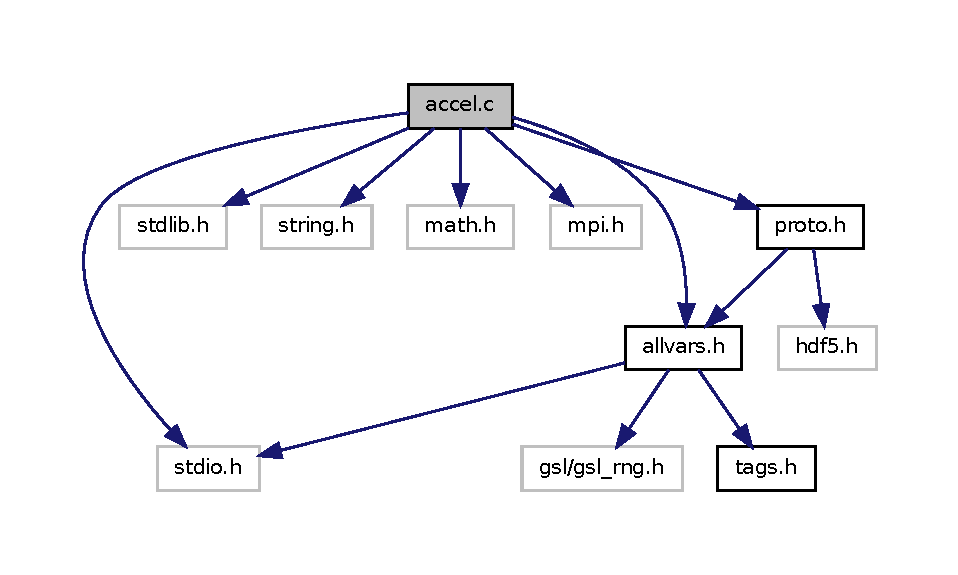
\includegraphics[width=400pt]{accel_8c__incl}
\end{center}
\end{figure}
\subsection*{Functions}
\begin{DoxyCompactItemize}
\item 
void \hyperlink{accel_8c_a147f9422f4bca4666608da992486b417}{compute\_\-accelerations} (int mode)
\end{DoxyCompactItemize}


\subsection{Detailed Description}
driver routine to carry out force computation 

Definition in file \hyperlink{accel_8c_source}{accel.c}.



\subsection{Function Documentation}
\hypertarget{accel_8c_a147f9422f4bca4666608da992486b417}{
\index{accel.c@{accel.c}!compute\_\-accelerations@{compute\_\-accelerations}}
\index{compute\_\-accelerations@{compute\_\-accelerations}!accel.c@{accel.c}}
\subsubsection[{compute\_\-accelerations}]{\setlength{\rightskip}{0pt plus 5cm}void compute\_\-accelerations (
\begin{DoxyParamCaption}
\item[{int}]{ mode}
\end{DoxyParamCaption}
)}}
\label{accel_8c_a147f9422f4bca4666608da992486b417}
This routine computes the accelerations for all active particles. First, the long-\/range PM force is computed if the TreePM algorithm is used and a \char`\"{}big\char`\"{} PM step is done. Next, the gravitational tree forces are computed. This also constructs the tree, if needed.

If gas particles are present, the density-\/loop for active SPH particles is carried out. This includes an iteration on the correct number of neighbours. Finally, the hydrodynamical forces are added. 

Definition at line 24 of file accel.c.



References All, global\_\-data\_\-all\_\-processes::CPU\_\-Gravity, global\_\-data\_\-all\_\-processes::CPU\_\-Hydro, global\_\-data\_\-all\_\-processes::CPU\_\-PM, global\_\-data\_\-all\_\-processes::CPU\_\-Predict, density(), force\_\-update\_\-hmax(), gravity\_\-forcetest(), gravity\_\-tree(), hydro\_\-force(), long\_\-range\_\-force(), global\_\-data\_\-all\_\-processes::PM\_\-Ti\_\-endstep, second(), ThisTask, global\_\-data\_\-all\_\-processes::Ti\_\-Current, timediff(), global\_\-data\_\-all\_\-processes::TotN\_\-gas, and global\_\-data\_\-all\_\-processes::TypeOfOpeningCriterion.



Referenced by run().




\begin{DoxyCode}
{
  double tstart, tend;

  if(ThisTask == 0)
    {
      printf("Start force computation...\n");
      fflush(stdout);
    }

#ifdef PMGRID
  if(All.PM_Ti_endstep == All.Ti_Current)
    {
      tstart = second();
      long_range_force();
      tend = second();
      All.CPU_PM += timediff(tstart, tend);
    }
#endif

  tstart = second();            /* measure the time for the full force computatio
      n */

  gravity_tree();               /* computes gravity accel. */

  if(All.TypeOfOpeningCriterion == 1 && All.Ti_Current == 0)
    gravity_tree();             /* For the first timestep, we redo it
                                 * to allow usage of relative opening
                                 * criterion for consistent accuracy.
                                 */
  tend = second();
  All.CPU_Gravity += timediff(tstart, tend);

#ifdef FORCETEST
  gravity_forcetest();
#endif

  if(All.TotN_gas > 0)
    {
      if(ThisTask == 0)
        {
          printf("Start density computation...\n");
          fflush(stdout);
        }

      tstart = second();
      density();                /* computes density, and pressure */
      tend = second();
      All.CPU_Hydro += timediff(tstart, tend);

      tstart = second();
      force_update_hmax();      /* tell the tree nodes the new SPH smoothing leng
      th such that they are guaranteed to hold the correct max(Hsml) */
      tend = second();
      All.CPU_Predict += timediff(tstart, tend);


      if(ThisTask == 0)
        {
          printf("Start hydro-force computation...\n");
          fflush(stdout);
        }

      tstart = second();
      hydro_force();            /* adds hydrodynamical accelerations and computes
       viscous entropy injection  */
      tend = second();
      All.CPU_Hydro += timediff(tstart, tend);
    }

  if(ThisTask == 0)
    {
      printf("force computation done.\n");
      fflush(stdout);
    }
}
\end{DoxyCode}




Here is the call graph for this function:
\nopagebreak
\begin{figure}[H]
\begin{center}
\leavevmode
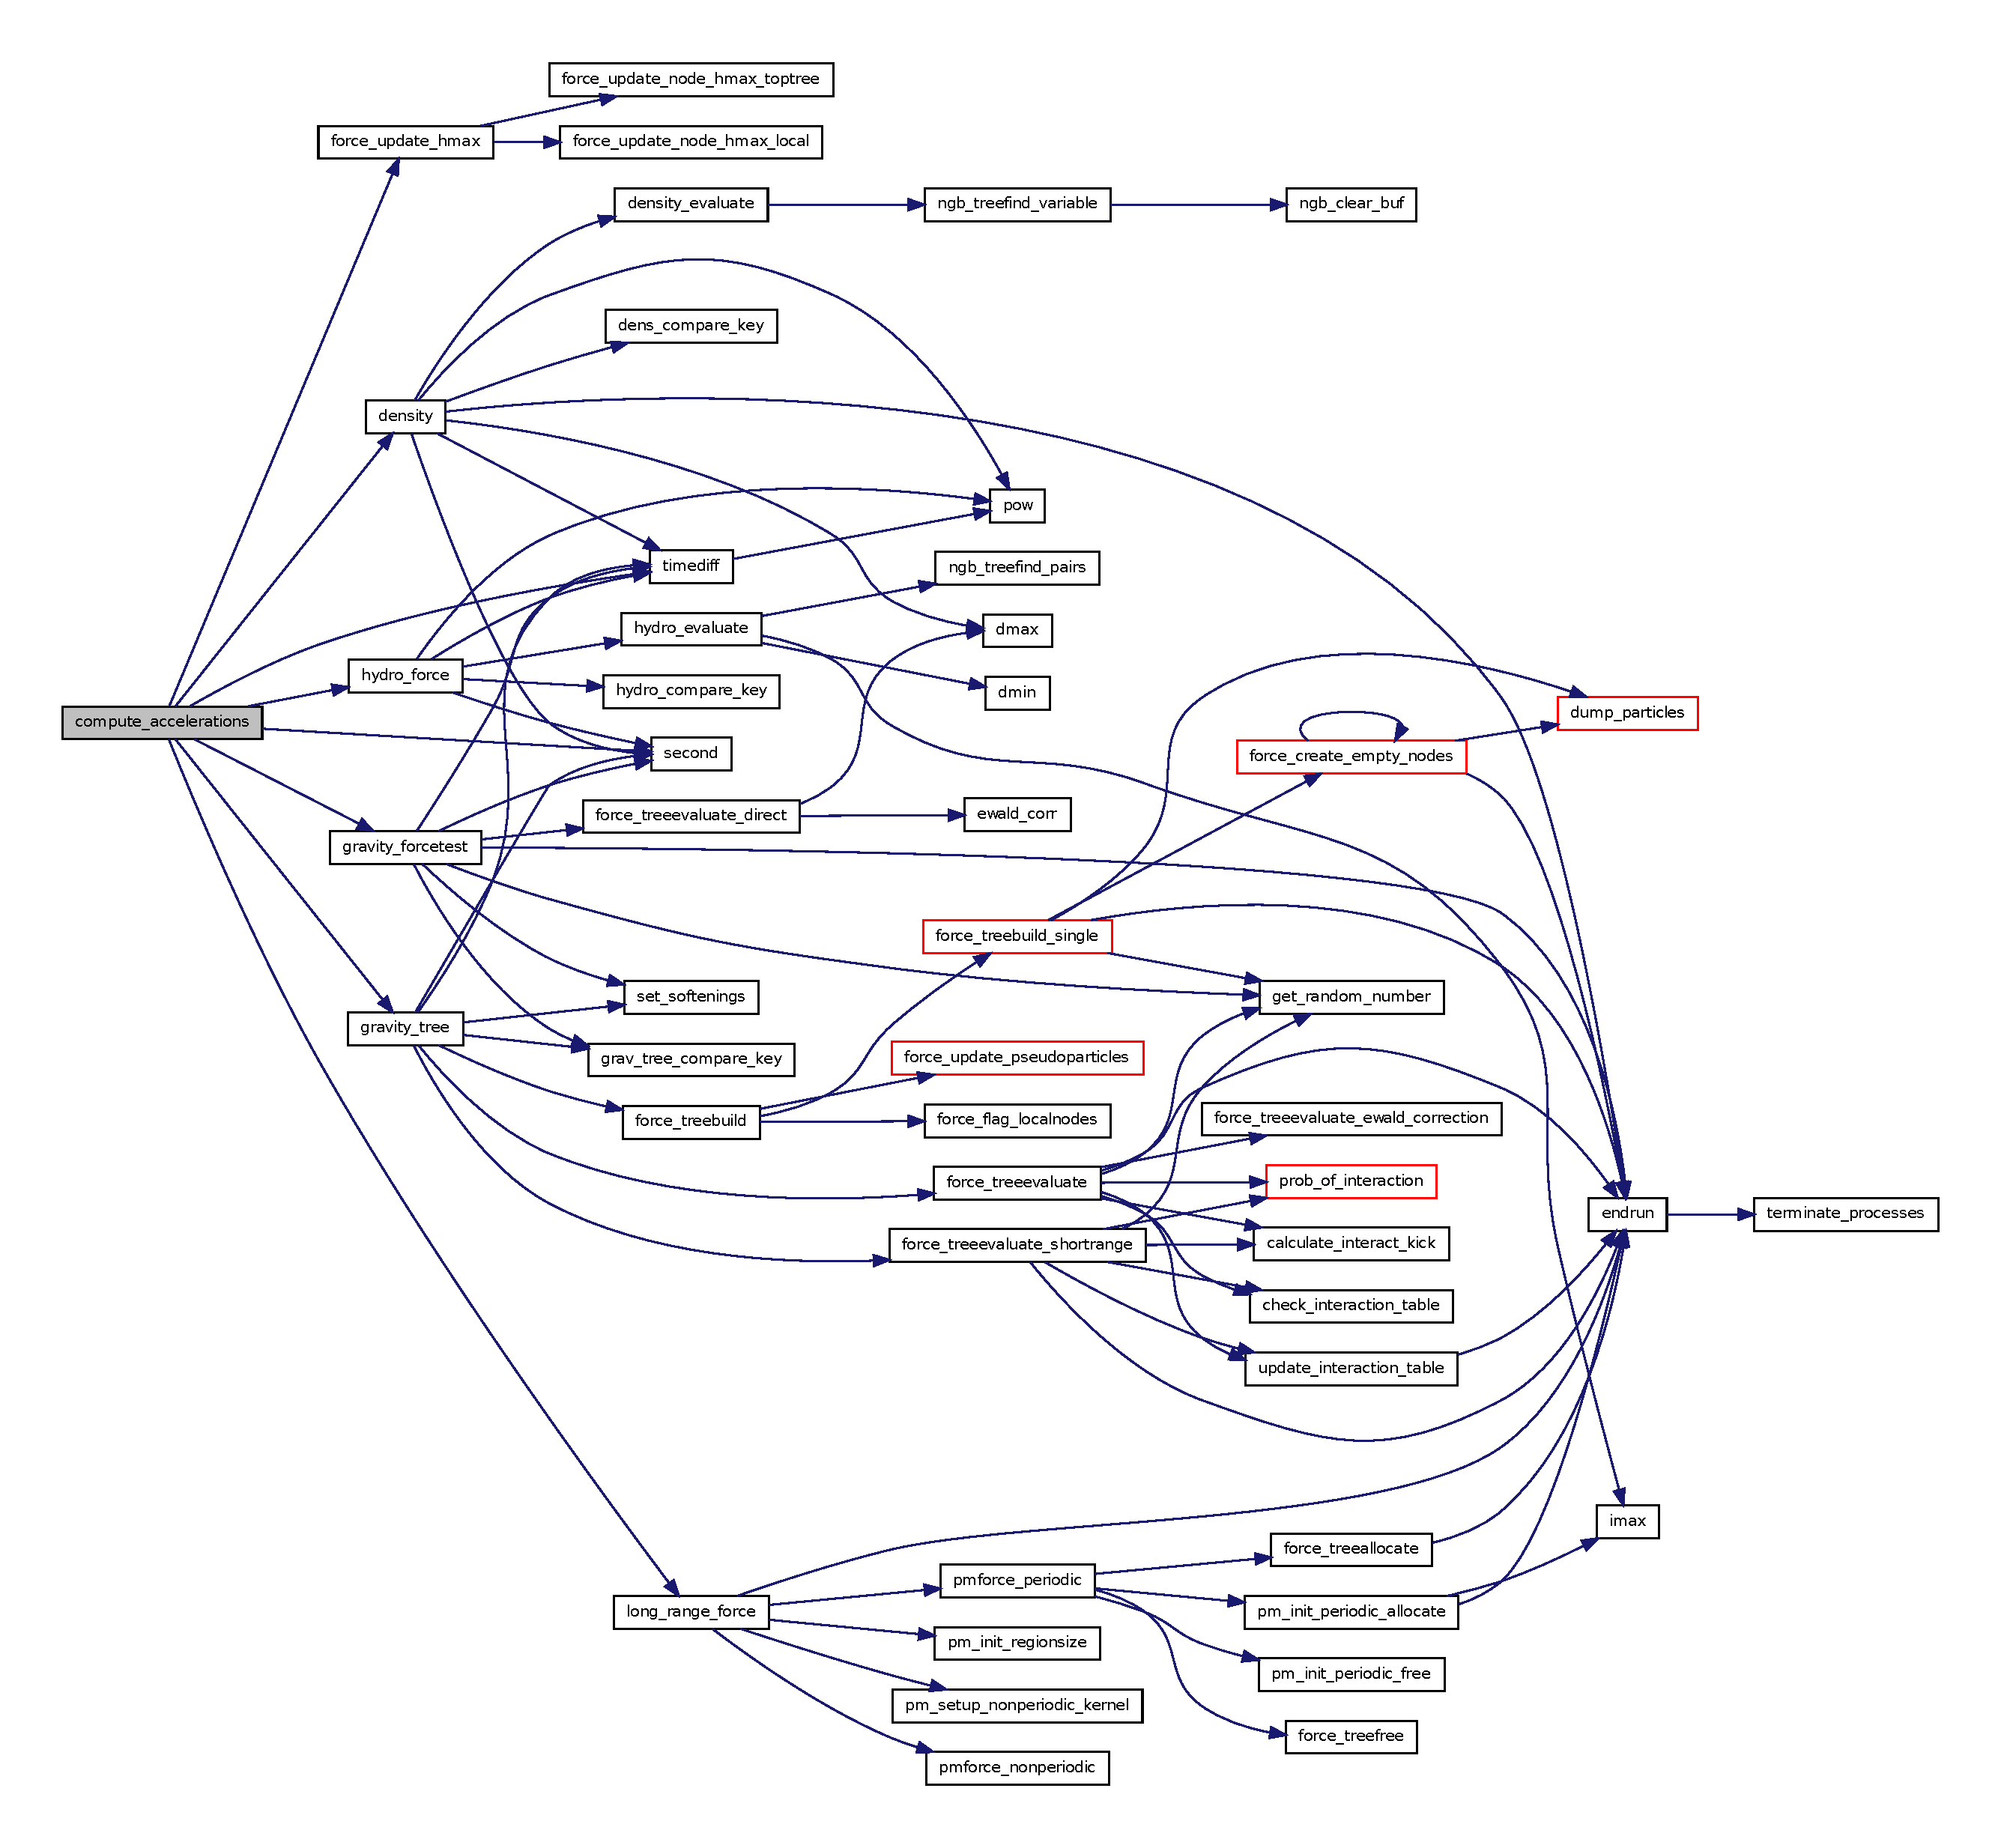
\includegraphics[width=400pt]{accel_8c_a147f9422f4bca4666608da992486b417_cgraph}
\end{center}
\end{figure}




Here is the caller graph for this function:\nopagebreak
\begin{figure}[H]
\begin{center}
\leavevmode
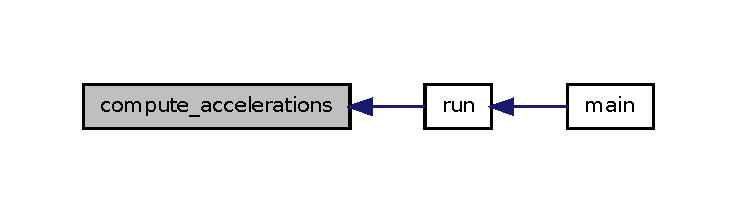
\includegraphics[width=354pt]{accel_8c_a147f9422f4bca4666608da992486b417_icgraph}
\end{center}
\end{figure}



\hypertarget{allocate_8c}{
\section{allocate.c File Reference}
\label{allocate_8c}\index{allocate.c@{allocate.c}}
}


routines for allocating particle and tree storage  


{\ttfamily \#include $<$stdio.h$>$}\par
{\ttfamily \#include $<$stdlib.h$>$}\par
{\ttfamily \#include $<$string.h$>$}\par
{\ttfamily \#include $<$math.h$>$}\par
{\ttfamily \#include \char`\"{}allvars.h\char`\"{}}\par
{\ttfamily \#include \char`\"{}proto.h\char`\"{}}\par
Include dependency graph for allocate.c:
\nopagebreak
\begin{figure}[H]
\begin{center}
\leavevmode
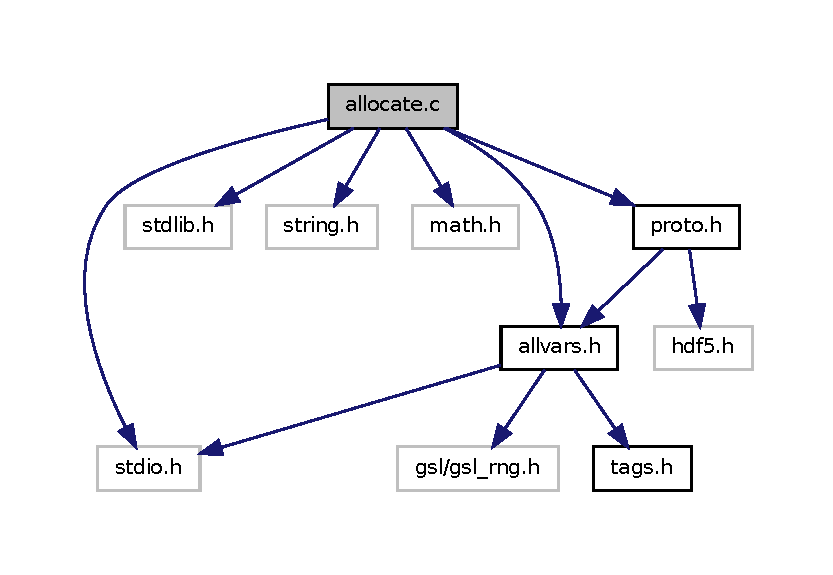
\includegraphics[width=400pt]{allocate_8c__incl}
\end{center}
\end{figure}
\subsection*{Functions}
\begin{DoxyCompactItemize}
\item 
void \hyperlink{allocate_8c_a9e761db39213af33ba28aeed461f1a5a}{allocate\_\-commbuffers} (void)
\item 
void \hyperlink{allocate_8c_a7fe5e304baaf5f418a22fef9a9cc02c7}{allocate\_\-memory} (void)
\item 
void \hyperlink{allocate_8c_a99877ff0dc6228eabf8f959569f2771e}{free\_\-memory} (void)
\end{DoxyCompactItemize}


\subsection{Detailed Description}
routines for allocating particle and tree storage 

Definition in file \hyperlink{allocate_8c_source}{allocate.c}.



\subsection{Function Documentation}
\hypertarget{allocate_8c_a9e761db39213af33ba28aeed461f1a5a}{
\index{allocate.c@{allocate.c}!allocate\_\-commbuffers@{allocate\_\-commbuffers}}
\index{allocate\_\-commbuffers@{allocate\_\-commbuffers}!allocate.c@{allocate.c}}
\subsubsection[{allocate\_\-commbuffers}]{\setlength{\rightskip}{0pt plus 5cm}void allocate\_\-commbuffers (
\begin{DoxyParamCaption}
\item[{void}]{}
\end{DoxyParamCaption}
)}}
\label{allocate_8c_a9e761db39213af33ba28aeed461f1a5a}
Allocates a number of small buffers and arrays, the largest one being the communication buffer. The communication buffer itself is mapped onto various tables used in the different parts of the force algorithms. We further allocate space for the top-\/level tree nodes, and auxiliary arrays for the domain decomposition algorithm. 

$<$ Maximum number of nodes in the top-\/level tree used for domain decomposition

$<$ Maximum number of nodes in the top-\/level tree used for domain decomposition

$<$ Maximum number of nodes in the top-\/level tree used for domain decomposition

$<$ Maximum number of nodes in the top-\/level tree used for domain decomposition

$<$ Maximum number of nodes in the top-\/level tree used for domain decomposition

$<$ Maximum number of nodes in the top-\/level tree used for domain decomposition

$<$ Maximum number of nodes in the top-\/level tree used for domain decomposition

$<$ Maximum number of nodes in the top-\/level tree used for domain decomposition

$<$ Maximum number of nodes in the top-\/level tree used for domain decomposition 



Definition at line 19 of file allocate.c.



References All, global\_\-data\_\-all\_\-processes::BufferSize, global\_\-data\_\-all\_\-processes::BunchSizeDensity, global\_\-data\_\-all\_\-processes::BunchSizeDomain, global\_\-data\_\-all\_\-processes::BunchSizeForce, global\_\-data\_\-all\_\-processes::BunchSizeHydro, CommBuffer, DensDataGet, DensDataIn, DensDataPartialResult, DensDataResult, DomainCount, DomainCountSph, DomainEndList, DomainHmax, DomainKeyBuf, DomainMoment, DomainNodeIndex, DomainPartBuf, DomainSphBuf, DomainStartList, DomainTask, DomainTreeNodeLen, DomainWork, endrun(), Exportflag, FLOAT, GravDataGet, GravDataIn, GravDataIndexTable, GravDataOut, GravDataResult, HydroDataGet, HydroDataIn, HydroDataPartialResult, HydroDataResult, MAXTOPNODES, NTask, ThisTask, and TopNodes.



Referenced by begrun().




\begin{DoxyCode}
{
  size_t bytes;

  Exportflag = malloc(NTask * sizeof(char));
  DomainStartList = malloc(NTask * sizeof(int));
  DomainEndList = malloc(NTask * sizeof(int));

  TopNodes = malloc(MAXTOPNODES * sizeof(struct topnode_data));

  DomainWork = malloc(MAXTOPNODES * sizeof(double));
  DomainCount = malloc(MAXTOPNODES * sizeof(int));
  DomainCountSph = malloc(MAXTOPNODES * sizeof(int));
  DomainTask = malloc(MAXTOPNODES * sizeof(int));
  DomainNodeIndex = malloc(MAXTOPNODES * sizeof(int));
  DomainTreeNodeLen = malloc(MAXTOPNODES * sizeof(FLOAT));
  DomainHmax = malloc(MAXTOPNODES * sizeof(FLOAT));
  DomainMoment = malloc(MAXTOPNODES * sizeof(struct DomainNODE));

  if(!(CommBuffer = malloc(bytes = All.BufferSize * 1024 * 1024)))
    {
      printf("failed to allocate memory for `CommBuffer' (%g MB).\n", bytes / (10
      24.0 * 1024.0));
      endrun(2);
    }

  All.BunchSizeForce =
    (All.BufferSize * 1024 * 1024) / (sizeof(struct gravdata_index) + 2 * sizeof(
      struct gravdata_in));

  if(All.BunchSizeForce & 1)
    All.BunchSizeForce -= 1;    /* make sure that All.BunchSizeForce is an even n
      umber 
                                   --> 8-byte alignment for 64bit processors */

  GravDataIndexTable = (struct gravdata_index *) CommBuffer;
  GravDataIn = (struct gravdata_in *) (GravDataIndexTable + All.BunchSizeForce);
  GravDataGet = GravDataIn + All.BunchSizeForce;
  GravDataOut = GravDataIn;     /* this will overwrite the GravDataIn-Table */
  GravDataResult = GravDataGet; /* this will overwrite the GravDataGet-Table */


  All.BunchSizeDensity =
    (All.BufferSize * 1024 * 1024) / (2 * sizeof(struct densdata_in) + 2 * sizeof
      (struct densdata_out));

  DensDataIn = (struct densdata_in *) CommBuffer;
  DensDataGet = DensDataIn + All.BunchSizeDensity;
  DensDataResult = (struct densdata_out *) (DensDataGet + All.BunchSizeDensity);
  DensDataPartialResult = DensDataResult + All.BunchSizeDensity;

  All.BunchSizeHydro =
    (All.BufferSize * 1024 * 1024) / (2 * sizeof(struct hydrodata_in) + 2 * sizeo
      f(struct hydrodata_out));

  HydroDataIn = (struct hydrodata_in *) CommBuffer;
  HydroDataGet = HydroDataIn + All.BunchSizeHydro;
  HydroDataResult = (struct hydrodata_out *) (HydroDataGet + All.BunchSizeHydro);
      
  HydroDataPartialResult = HydroDataResult + All.BunchSizeHydro;

  All.BunchSizeDomain =
    (All.BufferSize * 1024 * 1024) / (sizeof(struct particle_data) + sizeof(struc
      t sph_particle_data) +
                                      sizeof(peanokey));

  if(All.BunchSizeDomain & 1)
    All.BunchSizeDomain -= 1;   /* make sure that All.BunchSizeDomain is even 
                                   --> 8-byte alignment of DomainKeyBuf for 64bit
       processors */

  DomainPartBuf = (struct particle_data *) CommBuffer;
  DomainSphBuf = (struct sph_particle_data *) (DomainPartBuf + All.
      BunchSizeDomain);
  DomainKeyBuf = (peanokey *) (DomainSphBuf + All.BunchSizeDomain);


  if(ThisTask == 0)
    {
      printf("\nAllocated %d MByte communication buffer per processor.\n\n", All.
      BufferSize);
      printf("Communication buffer has room for %d particles in gravity computati
      on\n", All.BunchSizeForce);
      printf("Communication buffer has room for %d particles in density computati
      on\n", All.BunchSizeDensity);
      printf("Communication buffer has room for %d particles in hydro computation
      \n", All.BunchSizeHydro);
      printf("Communication buffer has room for %d particles in domain decomposit
      ion\n", All.BunchSizeDomain);
      printf("\n");
    }
}
\end{DoxyCode}




Here is the call graph for this function:
\nopagebreak
\begin{figure}[H]
\begin{center}
\leavevmode
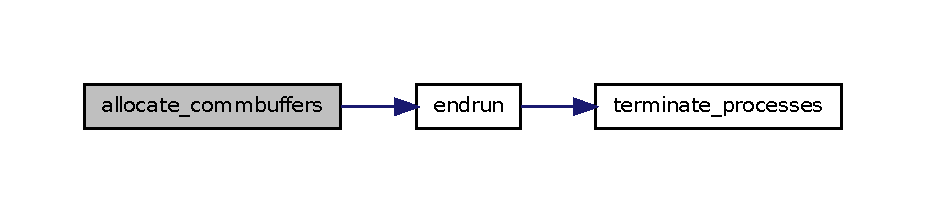
\includegraphics[width=400pt]{allocate_8c_a9e761db39213af33ba28aeed461f1a5a_cgraph}
\end{center}
\end{figure}




Here is the caller graph for this function:
\nopagebreak
\begin{figure}[H]
\begin{center}
\leavevmode
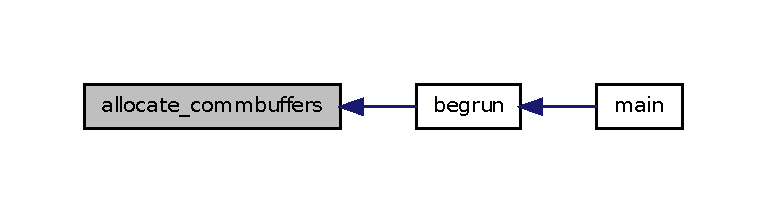
\includegraphics[width=368pt]{allocate_8c_a9e761db39213af33ba28aeed461f1a5a_icgraph}
\end{center}
\end{figure}


\hypertarget{allocate_8c_a7fe5e304baaf5f418a22fef9a9cc02c7}{
\index{allocate.c@{allocate.c}!allocate\_\-memory@{allocate\_\-memory}}
\index{allocate\_\-memory@{allocate\_\-memory}!allocate.c@{allocate.c}}
\subsubsection[{allocate\_\-memory}]{\setlength{\rightskip}{0pt plus 5cm}void allocate\_\-memory (
\begin{DoxyParamCaption}
\item[{void}]{}
\end{DoxyParamCaption}
)}}
\label{allocate_8c_a7fe5e304baaf5f418a22fef9a9cc02c7}
This routine allocates memory for particle storage, both the collisionless and the SPH particles. 

Definition at line 103 of file allocate.c.



References All, endrun(), global\_\-data\_\-all\_\-processes::MaxPart, global\_\-data\_\-all\_\-processes::MaxPartSph, P, SphP, and ThisTask.



Referenced by read\_\-file(), and restart().




\begin{DoxyCode}
{
  size_t bytes;
  double bytes_tot = 0;

  if(All.MaxPart > 0)
    {
      if(!(P = malloc(bytes = All.MaxPart * sizeof(struct particle_data))))
        {
          printf("failed to allocate memory for `P' (%g MB).\n", bytes / (1024.0 
      * 1024.0));
          endrun(1);
        }
      bytes_tot += bytes;

      if(ThisTask == 0)
        printf("\nAllocated %g MByte for particle storage. %lu\n\n", bytes_tot / 
      (1024.0 * 1024.0), sizeof(struct particle_data));
    }

  if(All.MaxPartSph > 0)
    {
      bytes_tot = 0;

      if(!(SphP = malloc(bytes = All.MaxPartSph * sizeof(struct 
      sph_particle_data))))
        {
          printf("failed to allocate memory for `SphP' (%g MB) %lu.\n", bytes / (
      1024.0 * 1024.0), sizeof(struct sph_particle_data));
          endrun(1);
        }
      bytes_tot += bytes;

      if(ThisTask == 0)
        printf("Allocated %g MByte for storage of SPH data. %lu\n\n", bytes_tot /
       (1024.0 * 1024.0), sizeof(struct sph_particle_data));
    }
}
\end{DoxyCode}




Here is the call graph for this function:
\nopagebreak
\begin{figure}[H]
\begin{center}
\leavevmode
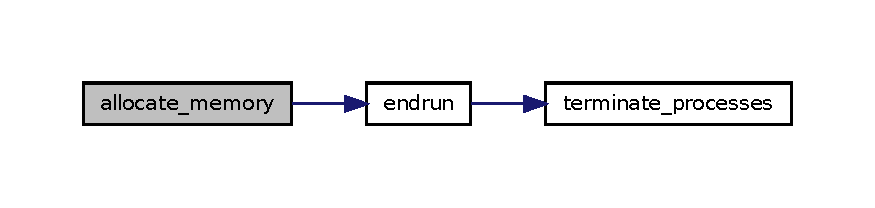
\includegraphics[width=400pt]{allocate_8c_a7fe5e304baaf5f418a22fef9a9cc02c7_cgraph}
\end{center}
\end{figure}




Here is the caller graph for this function:
\nopagebreak
\begin{figure}[H]
\begin{center}
\leavevmode
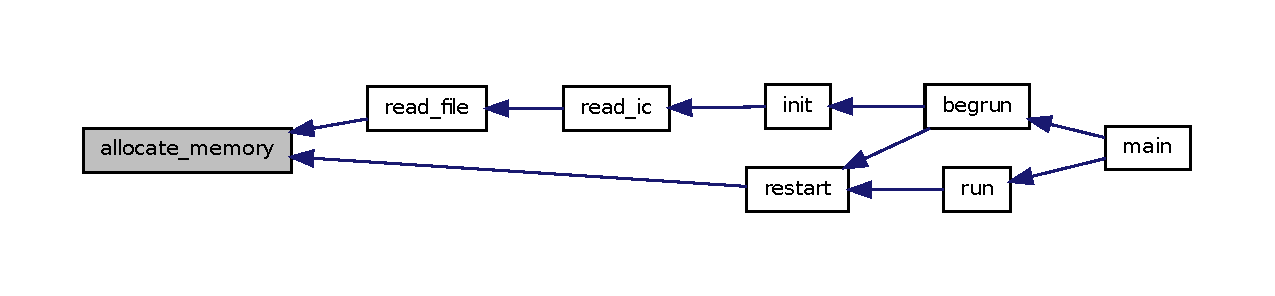
\includegraphics[width=400pt]{allocate_8c_a7fe5e304baaf5f418a22fef9a9cc02c7_icgraph}
\end{center}
\end{figure}


\hypertarget{allocate_8c_a99877ff0dc6228eabf8f959569f2771e}{
\index{allocate.c@{allocate.c}!free\_\-memory@{free\_\-memory}}
\index{free\_\-memory@{free\_\-memory}!allocate.c@{allocate.c}}
\subsubsection[{free\_\-memory}]{\setlength{\rightskip}{0pt plus 5cm}void free\_\-memory (
\begin{DoxyParamCaption}
\item[{void}]{}
\end{DoxyParamCaption}
)}}
\label{allocate_8c_a99877ff0dc6228eabf8f959569f2771e}
This routine frees the memory for the particle storage. Note: We don't actually bother to call it in the code... When the program terminats, the memory will be automatically freed by the operating system. 

Definition at line 144 of file allocate.c.



References All, global\_\-data\_\-all\_\-processes::MaxPart, global\_\-data\_\-all\_\-processes::MaxPartSph, P, and SphP.




\begin{DoxyCode}
{
  if(All.MaxPartSph > 0)
    free(SphP);

  if(All.MaxPart > 0)
    free(P);
}
\end{DoxyCode}



\hypertarget{allvars_8c}{
\section{allvars.c File Reference}
\label{allvars_8c}\index{allvars.c@{allvars.c}}
}


provides instances of all global variables.  


{\ttfamily \#include $<$stdio.h$>$}\par
{\ttfamily \#include $<$gsl/gsl\_\-rng.h$>$}\par
{\ttfamily \#include \char`\"{}tags.h\char`\"{}}\par
{\ttfamily \#include \char`\"{}allvars.h\char`\"{}}\par
Include dependency graph for allvars.c:\nopagebreak
\begin{figure}[H]
\begin{center}
\leavevmode
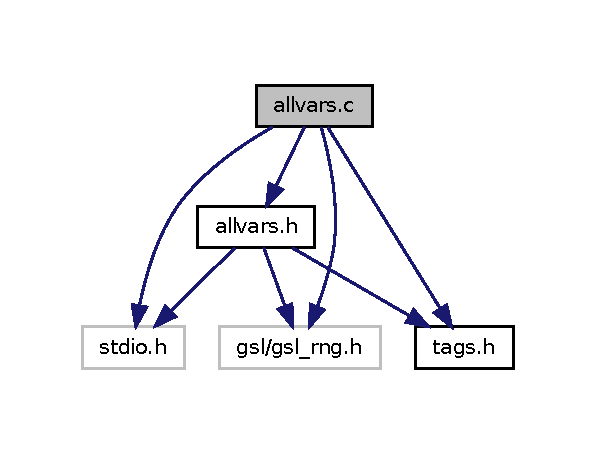
\includegraphics[width=286pt]{allvars_8c__incl}
\end{center}
\end{figure}
\subsection*{Variables}
\begin{DoxyCompactItemize}
\item 
int \hyperlink{allvars_8c_a52c8c7d2abff436111942e02c5bb466a}{ThisTask}
\item 
int \hyperlink{allvars_8c_a675acdcd149f5993271a1fdc11673b65}{NTask}
\item 
int \hyperlink{allvars_8c_a9a18606803f69f24d3cb2864640c122e}{PTask}
\item 
int \hyperlink{allvars_8c_a9ec69b53278f9bbe12890e50299026af}{NumPart}
\item 
int \hyperlink{allvars_8c_a8312e7470883d71db46cda5f1e616974}{N\_\-gas}
\item 
long long \hyperlink{allvars_8c_a697577a2a59bfa869161211cb134a6ae}{Ntype} \mbox{[}6\mbox{]}
\item 
int \hyperlink{allvars_8c_a7e6cdb6eab38cb043edcf56a4518dfca}{NtypeLocal} \mbox{[}6\mbox{]}
\item 
int \hyperlink{allvars_8c_a4c8b412a9883b4f6e0e8962ba54fd4ef}{NumForceUpdate}
\item 
int \hyperlink{allvars_8c_a0da112f9d57d7d936055dbb1035cd7fa}{NumSphUpdate}
\item 
double \hyperlink{allvars_8c_a2550e86a899b36eaf7428b23f98a05ec}{CPUThisRun}
\item 
int \hyperlink{allvars_8c_a7f2decfd266dfa9b4560409b9e72b4ab}{RestartFlag}
\item 
char $\ast$ \hyperlink{allvars_8c_a768b23818449e1b33a55747cb3cc2025}{Exportflag}
\item 
int $\ast$ \hyperlink{allvars_8c_ade1b96e6772d0d1ccb06bcbec352b5bd}{Ngblist}
\item 
int \hyperlink{allvars_8c_aa32d7269f9baf3ffdbdd509982fca128}{TreeReconstructFlag}
\item 
int \hyperlink{allvars_8c_a6343a9f3619e77c1796309b8deda7f50}{Flag\_\-FullStep}
\item 
gsl\_\-rng $\ast$ \hyperlink{allvars_8c_a4ec93729b85eb5da23dd6ffb23c3702b}{random\_\-generator}
\item 
double \hyperlink{allvars_8c_aa91f67a734086ebfa758994e579c80a9}{RndTable} \mbox{[}3000\mbox{]}
\item 
double \hyperlink{allvars_8c_a55dacf524ba7bbc5210fc68469a05d0f}{DomainCorner} \mbox{[}3\mbox{]}
\item 
double \hyperlink{allvars_8c_ad13aabcbb50307c005ffa0b2edccdaeb}{DomainCenter} \mbox{[}3\mbox{]}
\item 
double \hyperlink{allvars_8c_a3dd9593672bf68f0c36fa3e5451e9265}{DomainLen}
\item 
double \hyperlink{allvars_8c_a4488078cfcc203156f193c43a1d3a2ef}{DomainFac}
\item 
int \hyperlink{allvars_8c_a424b31dae72cd3331485d2fb6490c7ac}{DomainMyStart}
\item 
int \hyperlink{allvars_8c_ad6c1a01f55d5c8b7b642525118acbebe}{DomainMyLast}
\item 
int $\ast$ \hyperlink{allvars_8c_a3c2a7b96fe94b5151d568fe321888d23}{DomainStartList}
\item 
int $\ast$ \hyperlink{allvars_8c_abb42257c117a39d968334cd054c16dcf}{DomainEndList}
\item 
double $\ast$ \hyperlink{allvars_8c_aed1b2c641567602d5935709a6a05b363}{DomainWork}
\item 
int $\ast$ \hyperlink{allvars_8c_a743ddd39e492911973f9acd210df0c7c}{DomainCount}
\item 
int $\ast$ \hyperlink{allvars_8c_acfb9351c127127b0de4a310bf91974e4}{DomainCountSph}
\item 
int $\ast$ \hyperlink{allvars_8c_a6f4a30ea20d1347d14d2e32de91390bb}{DomainTask}
\item 
int $\ast$ \hyperlink{allvars_8c_acd2b211f08f9b7e83da8cb58bf3931a0}{DomainNodeIndex}
\item 
float $\ast$ \hyperlink{allvars_8c_a52e5390127f5298d6639b9399077bfbf}{DomainTreeNodeLen}
\item 
float $\ast$ \hyperlink{allvars_8c_a5a4689ebf26bc52b81819580362ef4dc}{DomainHmax}
\item 
struct \hyperlink{structDomainNODE}{DomainNODE} $\ast$ \hyperlink{allvars_8c_ad90674eef0b2180889d1620d5cc8672b}{DomainMoment}
\item 
\hyperlink{allvars_8h_a63f10772bd5776dcb4b6301f425e0d26}{peanokey} $\ast$ \hyperlink{allvars_8c_a6918a0815266193ad242888c455c5886}{DomainKeyBuf}
\item 
\hyperlink{allvars_8h_a63f10772bd5776dcb4b6301f425e0d26}{peanokey} $\ast$ \hyperlink{allvars_8c_a828333e1bfb5cffdb0e67942bbcd6cdb}{Key}
\item 
\hyperlink{allvars_8h_a63f10772bd5776dcb4b6301f425e0d26}{peanokey} $\ast$ \hyperlink{allvars_8c_a8b9ee62bf965346f051e19e013d998b4}{KeySorted}
\item 
int \hyperlink{allvars_8c_a269a1fc2bea249d93115b160fd42ee84}{NTopnodes}
\item 
int \hyperlink{allvars_8c_a820bd6735d7313b9e7a3dcbe6c2f93d4}{NTopleaves}
\item 
struct \hyperlink{structtopnode__data}{topnode\_\-data} $\ast$ \hyperlink{allvars_8c_a855acc131f2f1193f48d60fe63037e8c}{TopNodes}
\item 
double \hyperlink{allvars_8c_ae43d9623e3a2c88558e99ecf90948906}{TimeOfLastTreeConstruction}
\item 
char \hyperlink{allvars_8c_aad74b601033a4fe957c6129de6e8406c}{ParameterFile} \mbox{[}100\mbox{]}
\item 
FILE $\ast$ \hyperlink{allvars_8c_af26719ed46b19cc760b7b55c3cb9968c}{FdInfo}
\item 
FILE $\ast$ \hyperlink{allvars_8c_a0230903e40950ac42dbff71dddd12176}{FdEnergy}
\item 
FILE $\ast$ \hyperlink{allvars_8c_a603fc3e63a037dff4463c67aa7a4c91e}{FdTimings}
\item 
FILE $\ast$ \hyperlink{allvars_8c_a889700103f4f515009e98a7d789fd164}{FdCPU}
\item 
FILE $\ast$ \hyperlink{allvars_8c_ae16a08c18946ccba84c72541b51055dd}{FdForceTest}
\item 
double \hyperlink{allvars_8c_a074db1ef4adfe88a5f3b07eac8c1daae}{DriftTable} \mbox{[}1000\mbox{]}
\item 
double \hyperlink{allvars_8c_a38e5d8b595161f074f7fbede3a8fda66}{GravKickTable} \mbox{[}1000\mbox{]}
\item 
double \hyperlink{allvars_8c_a274a5737d1578d54d6f82130e3064771}{HydroKickTable} \mbox{[}1000\mbox{]}
\item 
void $\ast$ \hyperlink{allvars_8c_ab9d6a5a8cf4049ad304ea6d23d8efb09}{CommBuffer}
\item 
struct \hyperlink{structglobal__data__all__processes}{global\_\-data\_\-all\_\-processes} \hyperlink{allvars_8c_ad49123ae0461ffe61629a0d4cf2ba91f}{All}
\item 
struct \hyperlink{structparticle__data}{particle\_\-data} $\ast$ \hyperlink{allvars_8c_a29aa1b496fa7d42c32c4cae3c77aa068}{P}
\item 
struct \hyperlink{structparticle__data}{particle\_\-data} $\ast$ \hyperlink{allvars_8c_a386309bed4018948d42bc72ae4b5e1bb}{DomainPartBuf}
\item 
struct \hyperlink{structsph__particle__data}{sph\_\-particle\_\-data} $\ast$ \hyperlink{allvars_8c_a331d32b863e95f7d488a26ae38bda6af}{SphP}
\item 
struct \hyperlink{structsph__particle__data}{sph\_\-particle\_\-data} $\ast$ \hyperlink{allvars_8c_a6034b1d1d1f6fb31d07d2077914aa1fc}{DomainSphBuf}
\item 
int \hyperlink{allvars_8c_aca70a1751175167a36c1c6775a338bee}{MaxNodes}
\item 
int \hyperlink{allvars_8c_acf4151281b98d29aa500c5e56e66741f}{Numnodestree}
\item 
struct \hyperlink{structNODE}{NODE} $\ast$ \hyperlink{allvars_8c_a0cb940c6ac9331805bcc91b437c78e9a}{Nodes\_\-base}
\item 
struct \hyperlink{structNODE}{NODE} $\ast$ \hyperlink{allvars_8c_ac46f89ba3715dfa877c2e1b8822da657}{Nodes}
\item 
int $\ast$ \hyperlink{allvars_8c_ad14ab43f541f9c33cb9222ea018c1365}{Nextnode}
\item 
int $\ast$ \hyperlink{allvars_8c_ae1adfde6b271afd077130a64e6b85766}{Father}
\item 
struct \hyperlink{structextNODE}{extNODE} $\ast$ \hyperlink{allvars_8c_a57932378336b142ac6e6a9ddb60dce3f}{Extnodes\_\-base}
\item 
struct \hyperlink{structextNODE}{extNODE} $\ast$ \hyperlink{allvars_8c_a32df265d89a3353759d155bbfad4f3e6}{Extnodes}
\item 
struct \hyperlink{structio__header}{io\_\-header} \hyperlink{allvars_8c_a5d111aa83cef5894eea3939d815bb803}{header}
\item 
char \hyperlink{allvars_8c_ab0664df93d97f96270978b84eb6fb80c}{Tab\_\-IO\_\-Labels} \mbox{[}11\mbox{]}\mbox{[}4\mbox{]}
\item 
struct \hyperlink{structstate__of__system}{state\_\-of\_\-system} \hyperlink{allvars_8c_af53292602db23da91797b37daeb9b8ce}{SysState}
\item 
struct \hyperlink{structgravdata__in}{gravdata\_\-in} $\ast$ \hyperlink{allvars_8c_aeb6d889627ff712e7f0f30510842eb2c}{GravDataIn}
\item 
struct \hyperlink{structgravdata__in}{gravdata\_\-in} $\ast$ \hyperlink{allvars_8c_abc4ea40ab91f3e9288a0394c2544c65b}{GravDataGet}
\item 
struct \hyperlink{structgravdata__in}{gravdata\_\-in} $\ast$ \hyperlink{allvars_8c_a1aab0f29675c0745b5c2887e4791c070}{GravDataResult}
\item 
struct \hyperlink{structgravdata__in}{gravdata\_\-in} $\ast$ \hyperlink{allvars_8c_a7b537ba13fc3cfff5d6fbb245e892fb6}{GravDataOut}
\item 
struct \hyperlink{structgravdata__index}{gravdata\_\-index} $\ast$ \hyperlink{allvars_8c_a430ddb048d692102568b323d8ebe1812}{GravDataIndexTable}
\item 
struct \hyperlink{structdensdata__in}{densdata\_\-in} $\ast$ \hyperlink{allvars_8c_ae697d6f8bee6bc6d77eb68e46155aed6}{DensDataIn}
\item 
struct \hyperlink{structdensdata__in}{densdata\_\-in} $\ast$ \hyperlink{allvars_8c_aa2903f03b426e94ee0e7dbd08e281e3e}{DensDataGet}
\item 
struct \hyperlink{structdensdata__out}{densdata\_\-out} $\ast$ \hyperlink{allvars_8c_a85a5932e895f3ffca16cbfdb0b0d4b10}{DensDataResult}
\item 
struct \hyperlink{structdensdata__out}{densdata\_\-out} $\ast$ \hyperlink{allvars_8c_a6ba7d2763f0c08d5759c63d3ba44b3bd}{DensDataPartialResult}
\item 
struct \hyperlink{structhydrodata__in}{hydrodata\_\-in} $\ast$ \hyperlink{allvars_8c_ac76194e83ab629234cfbe7ea412f4147}{HydroDataIn}
\item 
struct \hyperlink{structhydrodata__in}{hydrodata\_\-in} $\ast$ \hyperlink{allvars_8c_a361f3970d23b525898314bd2742ecf8c}{HydroDataGet}
\item 
struct \hyperlink{structhydrodata__out}{hydrodata\_\-out} $\ast$ \hyperlink{allvars_8c_a4ec6a36a80786f2f8e7fb9794c1f6629}{HydroDataResult}
\item 
struct \hyperlink{structhydrodata__out}{hydrodata\_\-out} $\ast$ \hyperlink{allvars_8c_ab7f7e4c36b3ed818849ba610d82b38bc}{HydroDataPartialResult}
\end{DoxyCompactItemize}


\subsection{Detailed Description}
provides instances of all global variables. 

Definition in file \hyperlink{allvars_8c_source}{allvars.c}.



\subsection{Variable Documentation}
\hypertarget{allvars_8c_ad49123ae0461ffe61629a0d4cf2ba91f}{
\index{allvars.c@{allvars.c}!All@{All}}
\index{All@{All}!allvars.c@{allvars.c}}
\subsubsection[{All}]{\setlength{\rightskip}{0pt plus 5cm}struct {\bf global\_\-data\_\-all\_\-processes} {\bf All}}}
\label{allvars_8c_ad49123ae0461ffe61629a0d4cf2ba91f}
This structure contains data which is the SAME for all tasks (mostly code parameters read from the parameter file). Holding this data in a structure is convenient for writing/reading the restart file, and it allows the introduction of new global variables in a simple way. The only thing to do is to introduce them into this structure. 

Definition at line 112 of file allvars.c.



Referenced by advance\_\-and\_\-find\_\-timesteps(), allocate\_\-commbuffers(), allocate\_\-memory(), begrun(), check\_\-omega(), compute\_\-accelerations(), compute\_\-global\_\-quantities\_\-of\_\-system(), compute\_\-potential(), density(), density\_\-evaluate(), do\_\-box\_\-wrapping(), domain\_\-decompose(), domain\_\-Decomposition(), domain\_\-determineTopTree(), domain\_\-findExchangeNumbers(), domain\_\-topsplit(), domain\_\-topsplit\_\-local(), drift\_\-integ(), energy\_\-statistics(), every\_\-timestep\_\-stuff(), ewald\_\-init(), fill\_\-write\_\-buffer(), find\_\-dt\_\-displacement\_\-constraint(), find\_\-files(), find\_\-next\_\-outputtime(), find\_\-next\_\-sync\_\-point\_\-and\_\-drift(), force\_\-insert\_\-pseudo\_\-particles(), force\_\-treeallocate(), force\_\-treebuild(), force\_\-treebuild\_\-single(), force\_\-treeevaluate(), force\_\-treeevaluate\_\-direct(), force\_\-treeevaluate\_\-ewald\_\-correction(), force\_\-treeevaluate\_\-potential(), force\_\-treeevaluate\_\-potential\_\-shortrange(), force\_\-treeevaluate\_\-shortrange(), force\_\-treeupdate\_\-pseudos(), force\_\-update\_\-node\_\-recursive(), free\_\-memory(), get\_\-drift\_\-factor(), get\_\-gravkick\_\-factor(), get\_\-hydrokick\_\-factor(), get\_\-particles\_\-in\_\-block(), get\_\-timestep(), gravity\_\-forcetest(), gravity\_\-tree(), gravkick\_\-integ(), growthfactor\_\-integ(), hydro\_\-evaluate(), hydro\_\-force(), hydrokick\_\-integ(), init(), init\_\-drift\_\-table(), long\_\-range\_\-force(), main(), move\_\-particles(), ngb\_\-treeallocate(), ngb\_\-treefind\_\-pairs(), ngb\_\-treefind\_\-variable(), open\_\-outputfiles(), pm\_\-init\_\-periodic(), pmforce\_\-periodic(), pmpotential\_\-periodic(), prob\_\-of\_\-interaction(), read\_\-file(), read\_\-ic(), read\_\-outputlist(), read\_\-parameter\_\-file(), readjust\_\-timebase(), restart(), run(), savepositions(), set\_\-softenings(), set\_\-units(), setup\_\-smoothinglengths(), and write\_\-file().

\hypertarget{allvars_8c_ab9d6a5a8cf4049ad304ea6d23d8efb09}{
\index{allvars.c@{allvars.c}!CommBuffer@{CommBuffer}}
\index{CommBuffer@{CommBuffer}!allvars.c@{allvars.c}}
\subsubsection[{CommBuffer}]{\setlength{\rightskip}{0pt plus 5cm}void$\ast$ {\bf CommBuffer}}}
\label{allvars_8c_ab9d6a5a8cf4049ad304ea6d23d8efb09}
points to communication buffer, which is used in the domain decomposition, the parallel tree-\/force computation, the SPH routines, etc. 

Definition at line 102 of file allvars.c.



Referenced by allocate\_\-commbuffers(), empty\_\-read\_\-buffer(), fill\_\-write\_\-buffer(), read\_\-file(), and write\_\-file().

\hypertarget{allvars_8c_a2550e86a899b36eaf7428b23f98a05ec}{
\index{allvars.c@{allvars.c}!CPUThisRun@{CPUThisRun}}
\index{CPUThisRun@{CPUThisRun}!allvars.c@{allvars.c}}
\subsubsection[{CPUThisRun}]{\setlength{\rightskip}{0pt plus 5cm}double {\bf CPUThisRun}}}
\label{allvars_8c_a2550e86a899b36eaf7428b23f98a05ec}
Sums the CPU time for the process (current submission only) 

Definition at line 23 of file allvars.c.



Referenced by begrun(), main(), and run().

\hypertarget{allvars_8c_aa2903f03b426e94ee0e7dbd08e281e3e}{
\index{allvars.c@{allvars.c}!DensDataGet@{DensDataGet}}
\index{DensDataGet@{DensDataGet}!allvars.c@{allvars.c}}
\subsubsection[{DensDataGet}]{\setlength{\rightskip}{0pt plus 5cm}struct {\bf densdata\_\-in} $\ast$ {\bf DensDataGet}}}
\label{allvars_8c_aa2903f03b426e94ee0e7dbd08e281e3e}
holds imported particle data for SPH density computation 

Definition at line 191 of file allvars.c.



Referenced by allocate\_\-commbuffers(), density(), and density\_\-evaluate().

\hypertarget{allvars_8c_ae697d6f8bee6bc6d77eb68e46155aed6}{
\index{allvars.c@{allvars.c}!DensDataIn@{DensDataIn}}
\index{DensDataIn@{DensDataIn}!allvars.c@{allvars.c}}
\subsubsection[{DensDataIn}]{\setlength{\rightskip}{0pt plus 5cm}struct {\bf densdata\_\-in}$\ast$ {\bf DensDataIn}}}
\label{allvars_8c_ae697d6f8bee6bc6d77eb68e46155aed6}
holds particle data for SPH density computation to be exported to other processors 

Definition at line 191 of file allvars.c.



Referenced by allocate\_\-commbuffers(), and density().

\hypertarget{allvars_8c_a6ba7d2763f0c08d5759c63d3ba44b3bd}{
\index{allvars.c@{allvars.c}!DensDataPartialResult@{DensDataPartialResult}}
\index{DensDataPartialResult@{DensDataPartialResult}!allvars.c@{allvars.c}}
\subsubsection[{DensDataPartialResult}]{\setlength{\rightskip}{0pt plus 5cm}struct {\bf densdata\_\-out} $\ast$ {\bf DensDataPartialResult}}}
\label{allvars_8c_a6ba7d2763f0c08d5759c63d3ba44b3bd}
imported partial SPH density results from other processors 

Definition at line 195 of file allvars.c.



Referenced by allocate\_\-commbuffers(), and density().

\hypertarget{allvars_8c_a85a5932e895f3ffca16cbfdb0b0d4b10}{
\index{allvars.c@{allvars.c}!DensDataResult@{DensDataResult}}
\index{DensDataResult@{DensDataResult}!allvars.c@{allvars.c}}
\subsubsection[{DensDataResult}]{\setlength{\rightskip}{0pt plus 5cm}struct {\bf densdata\_\-out}$\ast$ {\bf DensDataResult}}}
\label{allvars_8c_a85a5932e895f3ffca16cbfdb0b0d4b10}
stores the locally computed SPH density results for imported particles 

Definition at line 195 of file allvars.c.



Referenced by allocate\_\-commbuffers(), density(), and density\_\-evaluate().

\hypertarget{allvars_8c_ad13aabcbb50307c005ffa0b2edccdaeb}{
\index{allvars.c@{allvars.c}!DomainCenter@{DomainCenter}}
\index{DomainCenter@{DomainCenter}!allvars.c@{allvars.c}}
\subsubsection[{DomainCenter}]{\setlength{\rightskip}{0pt plus 5cm}double {\bf DomainCenter}\mbox{[}3\mbox{]}}}
\label{allvars_8c_ad13aabcbb50307c005ffa0b2edccdaeb}
gives the center of simulation volume 

Definition at line 45 of file allvars.c.



Referenced by domain\_\-findExtent(), force\_\-treebuild\_\-single(), and restart().

\hypertarget{allvars_8c_a55dacf524ba7bbc5210fc68469a05d0f}{
\index{allvars.c@{allvars.c}!DomainCorner@{DomainCorner}}
\index{DomainCorner@{DomainCorner}!allvars.c@{allvars.c}}
\subsubsection[{DomainCorner}]{\setlength{\rightskip}{0pt plus 5cm}double {\bf DomainCorner}\mbox{[}3\mbox{]}}}
\label{allvars_8c_a55dacf524ba7bbc5210fc68469a05d0f}
gives the lower left corner of simulation volume 

Definition at line 44 of file allvars.c.



Referenced by domain\_\-determineTopTree(), domain\_\-findExtent(), force\_\-treebuild\_\-single(), and restart().

\hypertarget{allvars_8c_a743ddd39e492911973f9acd210df0c7c}{
\index{allvars.c@{allvars.c}!DomainCount@{DomainCount}}
\index{DomainCount@{DomainCount}!allvars.c@{allvars.c}}
\subsubsection[{DomainCount}]{\setlength{\rightskip}{0pt plus 5cm}int$\ast$ {\bf DomainCount}}}
\label{allvars_8c_a743ddd39e492911973f9acd210df0c7c}
a table that gives the total number of particles held by each processor 

Definition at line 53 of file allvars.c.



Referenced by allocate\_\-commbuffers(), domain\_\-findSplit(), domain\_\-shiftSplit(), and domain\_\-sumCost().

\hypertarget{allvars_8c_acfb9351c127127b0de4a310bf91974e4}{
\index{allvars.c@{allvars.c}!DomainCountSph@{DomainCountSph}}
\index{DomainCountSph@{DomainCountSph}!allvars.c@{allvars.c}}
\subsubsection[{DomainCountSph}]{\setlength{\rightskip}{0pt plus 5cm}int$\ast$ {\bf DomainCountSph}}}
\label{allvars_8c_acfb9351c127127b0de4a310bf91974e4}
a table that gives the total number of SPH particles held by each processor 

Definition at line 54 of file allvars.c.



Referenced by allocate\_\-commbuffers(), domain\_\-findSplit(), domain\_\-shiftSplit(), and domain\_\-sumCost().

\hypertarget{allvars_8c_abb42257c117a39d968334cd054c16dcf}{
\index{allvars.c@{allvars.c}!DomainEndList@{DomainEndList}}
\index{DomainEndList@{DomainEndList}!allvars.c@{allvars.c}}
\subsubsection[{DomainEndList}]{\setlength{\rightskip}{0pt plus 5cm}int$\ast$ {\bf DomainEndList}}}
\label{allvars_8c_abb42257c117a39d968334cd054c16dcf}
a table that lists the last domain mesh cell for all processors 

Definition at line 51 of file allvars.c.



Referenced by allocate\_\-commbuffers(), domain\_\-decompose(), domain\_\-findSplit(), domain\_\-shiftSplit(), force\_\-exchange\_\-pseudodata(), force\_\-update\_\-hmax(), force\_\-update\_\-len(), and restart().

\hypertarget{allvars_8c_a4488078cfcc203156f193c43a1d3a2ef}{
\index{allvars.c@{allvars.c}!DomainFac@{DomainFac}}
\index{DomainFac@{DomainFac}!allvars.c@{allvars.c}}
\subsubsection[{DomainFac}]{\setlength{\rightskip}{0pt plus 5cm}double {\bf DomainFac}}}
\label{allvars_8c_a4488078cfcc203156f193c43a1d3a2ef}
factor used for converting particle coordinates to a Peano-\/Hilbert mesh covering the simulation volume 

Definition at line 47 of file allvars.c.



Referenced by domain\_\-determineTopTree(), domain\_\-findExtent(), force\_\-treebuild\_\-single(), and restart().

\hypertarget{allvars_8c_a5a4689ebf26bc52b81819580362ef4dc}{
\index{allvars.c@{allvars.c}!DomainHmax@{DomainHmax}}
\index{DomainHmax@{DomainHmax}!allvars.c@{allvars.c}}
\subsubsection[{DomainHmax}]{\setlength{\rightskip}{0pt plus 5cm}float$\ast$ {\bf DomainHmax}}}
\label{allvars_8c_a5a4689ebf26bc52b81819580362ef4dc}
this table gives for each leaf of the top-\/level tree the maximum SPH smoothing length among the particles of the corresponding node of the gravitational tree 

Definition at line 59 of file allvars.c.



Referenced by allocate\_\-commbuffers(), force\_\-update\_\-hmax(), force\_\-update\_\-node\_\-hmax\_\-toptree(), and restart().

\hypertarget{allvars_8c_a6918a0815266193ad242888c455c5886}{
\index{allvars.c@{allvars.c}!DomainKeyBuf@{DomainKeyBuf}}
\index{DomainKeyBuf@{DomainKeyBuf}!allvars.c@{allvars.c}}
\subsubsection[{DomainKeyBuf}]{\setlength{\rightskip}{0pt plus 5cm}{\bf peanokey}$\ast$ {\bf DomainKeyBuf}}}
\label{allvars_8c_a6918a0815266193ad242888c455c5886}
this points to a buffer used during the exchange of particle data 

Definition at line 64 of file allvars.c.



Referenced by allocate\_\-commbuffers(), and domain\_\-exchangeParticles().

\hypertarget{allvars_8c_a3dd9593672bf68f0c36fa3e5451e9265}{
\index{allvars.c@{allvars.c}!DomainLen@{DomainLen}}
\index{DomainLen@{DomainLen}!allvars.c@{allvars.c}}
\subsubsection[{DomainLen}]{\setlength{\rightskip}{0pt plus 5cm}double {\bf DomainLen}}}
\label{allvars_8c_a3dd9593672bf68f0c36fa3e5451e9265}
gives the (maximum) side-\/length of simulation volume 

Definition at line 46 of file allvars.c.



Referenced by domain\_\-findExtent(), force\_\-treebuild\_\-single(), and restart().

\hypertarget{allvars_8c_ad90674eef0b2180889d1620d5cc8672b}{
\index{allvars.c@{allvars.c}!DomainMoment@{DomainMoment}}
\index{DomainMoment@{DomainMoment}!allvars.c@{allvars.c}}
\subsubsection[{DomainMoment}]{\setlength{\rightskip}{0pt plus 5cm}struct {\bf DomainNODE}$\ast$ {\bf DomainMoment}}}
\label{allvars_8c_ad90674eef0b2180889d1620d5cc8672b}
this table stores for each node of the top-\/level tree corresponding node data from the gravitational tree 

Definition at line 61 of file allvars.c.



Referenced by allocate\_\-commbuffers(), force\_\-exchange\_\-pseudodata(), force\_\-insert\_\-pseudo\_\-particles(), force\_\-treeupdate\_\-pseudos(), and restart().

\hypertarget{allvars_8c_ad6c1a01f55d5c8b7b642525118acbebe}{
\index{allvars.c@{allvars.c}!DomainMyLast@{DomainMyLast}}
\index{DomainMyLast@{DomainMyLast}!allvars.c@{allvars.c}}
\subsubsection[{DomainMyLast}]{\setlength{\rightskip}{0pt plus 5cm}int {\bf DomainMyLast}}}
\label{allvars_8c_ad6c1a01f55d5c8b7b642525118acbebe}
last domain mesh cell that resides on the local processor 

Definition at line 49 of file allvars.c.



Referenced by domain\_\-decompose(), force\_\-exchange\_\-pseudodata(), force\_\-flag\_\-localnodes(), force\_\-insert\_\-pseudo\_\-particles(), force\_\-treeupdate\_\-pseudos(), force\_\-update\_\-hmax(), force\_\-update\_\-len(), force\_\-update\_\-node\_\-hmax\_\-toptree(), force\_\-update\_\-node\_\-len\_\-toptree(), and restart().

\hypertarget{allvars_8c_a424b31dae72cd3331485d2fb6490c7ac}{
\index{allvars.c@{allvars.c}!DomainMyStart@{DomainMyStart}}
\index{DomainMyStart@{DomainMyStart}!allvars.c@{allvars.c}}
\subsubsection[{DomainMyStart}]{\setlength{\rightskip}{0pt plus 5cm}int {\bf DomainMyStart}}}
\label{allvars_8c_a424b31dae72cd3331485d2fb6490c7ac}
first domain mesh cell that resides on the local processor 

Definition at line 48 of file allvars.c.



Referenced by domain\_\-decompose(), force\_\-exchange\_\-pseudodata(), force\_\-flag\_\-localnodes(), force\_\-update\_\-hmax(), force\_\-update\_\-len(), and restart().

\hypertarget{allvars_8c_acd2b211f08f9b7e83da8cb58bf3931a0}{
\index{allvars.c@{allvars.c}!DomainNodeIndex@{DomainNodeIndex}}
\index{DomainNodeIndex@{DomainNodeIndex}!allvars.c@{allvars.c}}
\subsubsection[{DomainNodeIndex}]{\setlength{\rightskip}{0pt plus 5cm}int$\ast$ {\bf DomainNodeIndex}}}
\label{allvars_8c_acd2b211f08f9b7e83da8cb58bf3931a0}
this table gives for each leaf of the top-\/level tree the corresponding node of the gravitational tree 

Definition at line 57 of file allvars.c.



Referenced by allocate\_\-commbuffers(), force\_\-create\_\-empty\_\-nodes(), force\_\-exchange\_\-pseudodata(), force\_\-flag\_\-localnodes(), force\_\-insert\_\-pseudo\_\-particles(), force\_\-treebuild\_\-single(), force\_\-treeupdate\_\-pseudos(), force\_\-update\_\-hmax(), force\_\-update\_\-len(), force\_\-update\_\-node\_\-hmax\_\-toptree(), force\_\-update\_\-node\_\-len\_\-toptree(), and restart().

\hypertarget{allvars_8c_a386309bed4018948d42bc72ae4b5e1bb}{
\index{allvars.c@{allvars.c}!DomainPartBuf@{DomainPartBuf}}
\index{DomainPartBuf@{DomainPartBuf}!allvars.c@{allvars.c}}
\subsubsection[{DomainPartBuf}]{\setlength{\rightskip}{0pt plus 5cm}struct {\bf particle\_\-data} $\ast$ {\bf DomainPartBuf}}}
\label{allvars_8c_a386309bed4018948d42bc72ae4b5e1bb}
buffer for particle data used in domain decomposition 

Definition at line 120 of file allvars.c.



Referenced by allocate\_\-commbuffers(), and domain\_\-exchangeParticles().

\hypertarget{allvars_8c_a6034b1d1d1f6fb31d07d2077914aa1fc}{
\index{allvars.c@{allvars.c}!DomainSphBuf@{DomainSphBuf}}
\index{DomainSphBuf@{DomainSphBuf}!allvars.c@{allvars.c}}
\subsubsection[{DomainSphBuf}]{\setlength{\rightskip}{0pt plus 5cm}struct {\bf sph\_\-particle\_\-data} $\ast$ {\bf DomainSphBuf}}}
\label{allvars_8c_a6034b1d1d1f6fb31d07d2077914aa1fc}
buffer for SPH particle data in domain decomposition 

Definition at line 128 of file allvars.c.



Referenced by allocate\_\-commbuffers(), and domain\_\-exchangeParticles().

\hypertarget{allvars_8c_a3c2a7b96fe94b5151d568fe321888d23}{
\index{allvars.c@{allvars.c}!DomainStartList@{DomainStartList}}
\index{DomainStartList@{DomainStartList}!allvars.c@{allvars.c}}
\subsubsection[{DomainStartList}]{\setlength{\rightskip}{0pt plus 5cm}int$\ast$ {\bf DomainStartList}}}
\label{allvars_8c_a3c2a7b96fe94b5151d568fe321888d23}
a table that lists the first domain mesh cell for all processors 

Definition at line 50 of file allvars.c.



Referenced by allocate\_\-commbuffers(), domain\_\-decompose(), domain\_\-findSplit(), domain\_\-shiftSplit(), force\_\-exchange\_\-pseudodata(), force\_\-update\_\-hmax(), force\_\-update\_\-len(), and restart().

\hypertarget{allvars_8c_a6f4a30ea20d1347d14d2e32de91390bb}{
\index{allvars.c@{allvars.c}!DomainTask@{DomainTask}}
\index{DomainTask@{DomainTask}!allvars.c@{allvars.c}}
\subsubsection[{DomainTask}]{\setlength{\rightskip}{0pt plus 5cm}int$\ast$ {\bf DomainTask}}}
\label{allvars_8c_a6f4a30ea20d1347d14d2e32de91390bb}
this table gives for each leaf of the top-\/level tree the processor it was assigned to 

Definition at line 56 of file allvars.c.



Referenced by allocate\_\-commbuffers(), domain\_\-countToGo(), domain\_\-exchangeParticles(), domain\_\-findSplit(), domain\_\-shiftSplit(), force\_\-treeevaluate(), force\_\-treeevaluate\_\-ewald\_\-correction(), force\_\-treeevaluate\_\-potential(), force\_\-treeevaluate\_\-potential\_\-shortrange(), force\_\-treeevaluate\_\-shortrange(), ngb\_\-treefind\_\-pairs(), ngb\_\-treefind\_\-variable(), and restart().

\hypertarget{allvars_8c_a52e5390127f5298d6639b9399077bfbf}{
\index{allvars.c@{allvars.c}!DomainTreeNodeLen@{DomainTreeNodeLen}}
\index{DomainTreeNodeLen@{DomainTreeNodeLen}!allvars.c@{allvars.c}}
\subsubsection[{DomainTreeNodeLen}]{\setlength{\rightskip}{0pt plus 5cm}float$\ast$ {\bf DomainTreeNodeLen}}}
\label{allvars_8c_a52e5390127f5298d6639b9399077bfbf}
this table gives for each leaf of the top-\/level tree the side-\/length of the corresponding node of the gravitational tree 

Definition at line 58 of file allvars.c.



Referenced by allocate\_\-commbuffers(), force\_\-update\_\-len(), force\_\-update\_\-node\_\-len\_\-toptree(), and restart().

\hypertarget{allvars_8c_aed1b2c641567602d5935709a6a05b363}{
\index{allvars.c@{allvars.c}!DomainWork@{DomainWork}}
\index{DomainWork@{DomainWork}!allvars.c@{allvars.c}}
\subsubsection[{DomainWork}]{\setlength{\rightskip}{0pt plus 5cm}double$\ast$ {\bf DomainWork}}}
\label{allvars_8c_aed1b2c641567602d5935709a6a05b363}
a table that gives the total \char`\"{}work\char`\"{} due to the particles stored by each processor 

Definition at line 52 of file allvars.c.



Referenced by allocate\_\-commbuffers(), domain\_\-shiftSplit(), and domain\_\-sumCost().

\hypertarget{allvars_8c_a074db1ef4adfe88a5f3b07eac8c1daae}{
\index{allvars.c@{allvars.c}!DriftTable@{DriftTable}}
\index{DriftTable@{DriftTable}!allvars.c@{allvars.c}}
\subsubsection[{DriftTable}]{\setlength{\rightskip}{0pt plus 5cm}double {\bf DriftTable}\mbox{[}1000\mbox{]}}}
\label{allvars_8c_a074db1ef4adfe88a5f3b07eac8c1daae}
table for the cosmological drift factors 

Definition at line 98 of file allvars.c.



Referenced by get\_\-drift\_\-factor(), and init\_\-drift\_\-table().

\hypertarget{allvars_8c_a768b23818449e1b33a55747cb3cc2025}{
\index{allvars.c@{allvars.c}!Exportflag@{Exportflag}}
\index{Exportflag@{Exportflag}!allvars.c@{allvars.c}}
\subsubsection[{Exportflag}]{\setlength{\rightskip}{0pt plus 5cm}char$\ast$ {\bf Exportflag}}}
\label{allvars_8c_a768b23818449e1b33a55747cb3cc2025}
Buffer used for flagging whether a particle needs to be exported to another process 

Definition at line 30 of file allvars.c.



Referenced by allocate\_\-commbuffers(), compute\_\-potential(), density(), force\_\-treeevaluate(), force\_\-treeevaluate\_\-ewald\_\-correction(), force\_\-treeevaluate\_\-potential(), force\_\-treeevaluate\_\-potential\_\-shortrange(), force\_\-treeevaluate\_\-shortrange(), gravity\_\-forcetest(), gravity\_\-tree(), hydro\_\-force(), ngb\_\-treefind\_\-pairs(), and ngb\_\-treefind\_\-variable().

\hypertarget{allvars_8c_a32df265d89a3353759d155bbfad4f3e6}{
\index{allvars.c@{allvars.c}!Extnodes@{Extnodes}}
\index{Extnodes@{Extnodes}!allvars.c@{allvars.c}}
\subsubsection[{Extnodes}]{\setlength{\rightskip}{0pt plus 5cm}struct {\bf extNODE} $\ast$ {\bf Extnodes}}}
\label{allvars_8c_a32df265d89a3353759d155bbfad4f3e6}
provides shifted access to extended node information, parallel to Nodes/Nodes\_\-base 

Definition at line 152 of file allvars.c.



Referenced by advance\_\-and\_\-find\_\-timesteps(), force\_\-exchange\_\-pseudodata(), force\_\-treeallocate(), force\_\-treeupdate\_\-pseudos(), force\_\-update\_\-hmax(), force\_\-update\_\-node\_\-hmax\_\-local(), force\_\-update\_\-node\_\-hmax\_\-toptree(), force\_\-update\_\-node\_\-recursive(), move\_\-particles(), and ngb\_\-treefind\_\-pairs().

\hypertarget{allvars_8c_a57932378336b142ac6e6a9ddb60dce3f}{
\index{allvars.c@{allvars.c}!Extnodes\_\-base@{Extnodes\_\-base}}
\index{Extnodes\_\-base@{Extnodes\_\-base}!allvars.c@{allvars.c}}
\subsubsection[{Extnodes\_\-base}]{\setlength{\rightskip}{0pt plus 5cm}struct {\bf extNODE}$\ast$ {\bf Extnodes\_\-base}}}
\label{allvars_8c_a57932378336b142ac6e6a9ddb60dce3f}
$<$ this structure holds additional tree-\/node information which is not needed in the actual gravity computation points to the actual memory allocted for the extended node information 

Definition at line 152 of file allvars.c.



Referenced by force\_\-treeallocate(), force\_\-treefree(), and restart().

\hypertarget{allvars_8c_ae1adfde6b271afd077130a64e6b85766}{
\index{allvars.c@{allvars.c}!Father@{Father}}
\index{Father@{Father}!allvars.c@{allvars.c}}
\subsubsection[{Father}]{\setlength{\rightskip}{0pt plus 5cm}int$\ast$ {\bf Father}}}
\label{allvars_8c_ae1adfde6b271afd077130a64e6b85766}
gives parent node in tree 

Definition at line 149 of file allvars.c.



Referenced by advance\_\-and\_\-find\_\-timesteps(), force\_\-treeallocate(), force\_\-treefree(), force\_\-update\_\-node\_\-hmax\_\-local(), force\_\-update\_\-node\_\-len\_\-local(), force\_\-update\_\-node\_\-recursive(), restart(), and setup\_\-smoothinglengths().

\hypertarget{allvars_8c_a889700103f4f515009e98a7d789fd164}{
\index{allvars.c@{allvars.c}!FdCPU@{FdCPU}}
\index{FdCPU@{FdCPU}!allvars.c@{allvars.c}}
\subsubsection[{FdCPU}]{\setlength{\rightskip}{0pt plus 5cm}FILE$\ast$ {\bf FdCPU}}}
\label{allvars_8c_a889700103f4f515009e98a7d789fd164}
file handle for cpu.txt log-\/file. 

Definition at line 88 of file allvars.c.



Referenced by close\_\-outputfiles(), every\_\-timestep\_\-stuff(), and open\_\-outputfiles().

\hypertarget{allvars_8c_a0230903e40950ac42dbff71dddd12176}{
\index{allvars.c@{allvars.c}!FdEnergy@{FdEnergy}}
\index{FdEnergy@{FdEnergy}!allvars.c@{allvars.c}}
\subsubsection[{FdEnergy}]{\setlength{\rightskip}{0pt plus 5cm}FILE$\ast$ {\bf FdEnergy}}}
\label{allvars_8c_a0230903e40950ac42dbff71dddd12176}
file handle for energy.txt log-\/file. 

Definition at line 86 of file allvars.c.



Referenced by close\_\-outputfiles(), energy\_\-statistics(), and open\_\-outputfiles().

\hypertarget{allvars_8c_ae16a08c18946ccba84c72541b51055dd}{
\index{allvars.c@{allvars.c}!FdForceTest@{FdForceTest}}
\index{FdForceTest@{FdForceTest}!allvars.c@{allvars.c}}
\subsubsection[{FdForceTest}]{\setlength{\rightskip}{0pt plus 5cm}FILE$\ast$ {\bf FdForceTest}}}
\label{allvars_8c_ae16a08c18946ccba84c72541b51055dd}
file handle for forcetest.txt log-\/file. 

Definition at line 91 of file allvars.c.



Referenced by close\_\-outputfiles(), gravity\_\-forcetest(), and open\_\-outputfiles().

\hypertarget{allvars_8c_af26719ed46b19cc760b7b55c3cb9968c}{
\index{allvars.c@{allvars.c}!FdInfo@{FdInfo}}
\index{FdInfo@{FdInfo}!allvars.c@{allvars.c}}
\subsubsection[{FdInfo}]{\setlength{\rightskip}{0pt plus 5cm}FILE$\ast$ {\bf FdInfo}}}
\label{allvars_8c_af26719ed46b19cc760b7b55c3cb9968c}
file handle for info.txt log-\/file. 

Definition at line 85 of file allvars.c.



Referenced by close\_\-outputfiles(), every\_\-timestep\_\-stuff(), and open\_\-outputfiles().

\hypertarget{allvars_8c_a603fc3e63a037dff4463c67aa7a4c91e}{
\index{allvars.c@{allvars.c}!FdTimings@{FdTimings}}
\index{FdTimings@{FdTimings}!allvars.c@{allvars.c}}
\subsubsection[{FdTimings}]{\setlength{\rightskip}{0pt plus 5cm}FILE$\ast$ {\bf FdTimings}}}
\label{allvars_8c_a603fc3e63a037dff4463c67aa7a4c91e}
file handle for timings.txt log-\/file. 

Definition at line 87 of file allvars.c.



Referenced by close\_\-outputfiles(), gravity\_\-forcetest(), gravity\_\-tree(), and open\_\-outputfiles().

\hypertarget{allvars_8c_a6343a9f3619e77c1796309b8deda7f50}{
\index{allvars.c@{allvars.c}!Flag\_\-FullStep@{Flag\_\-FullStep}}
\index{Flag\_\-FullStep@{Flag\_\-FullStep}!allvars.c@{allvars.c}}
\subsubsection[{Flag\_\-FullStep}]{\setlength{\rightskip}{0pt plus 5cm}int {\bf Flag\_\-FullStep}}}
\label{allvars_8c_a6343a9f3619e77c1796309b8deda7f50}
This flag signals that the current step involves all particles 

Definition at line 36 of file allvars.c.



Referenced by advance\_\-and\_\-find\_\-timesteps(), find\_\-next\_\-sync\_\-point\_\-and\_\-drift(), and init().

\hypertarget{allvars_8c_abc4ea40ab91f3e9288a0394c2544c65b}{
\index{allvars.c@{allvars.c}!GravDataGet@{GravDataGet}}
\index{GravDataGet@{GravDataGet}!allvars.c@{allvars.c}}
\subsubsection[{GravDataGet}]{\setlength{\rightskip}{0pt plus 5cm}struct {\bf gravdata\_\-in} $\ast$ {\bf GravDataGet}}}
\label{allvars_8c_abc4ea40ab91f3e9288a0394c2544c65b}
holds particle data imported from other processors 

Definition at line 180 of file allvars.c.



Referenced by allocate\_\-commbuffers(), compute\_\-potential(), force\_\-treeevaluate(), force\_\-treeevaluate\_\-direct(), force\_\-treeevaluate\_\-potential(), force\_\-treeevaluate\_\-potential\_\-shortrange(), force\_\-treeevaluate\_\-shortrange(), gravity\_\-forcetest(), and gravity\_\-tree().

\hypertarget{allvars_8c_aeb6d889627ff712e7f0f30510842eb2c}{
\index{allvars.c@{allvars.c}!GravDataIn@{GravDataIn}}
\index{GravDataIn@{GravDataIn}!allvars.c@{allvars.c}}
\subsubsection[{GravDataIn}]{\setlength{\rightskip}{0pt plus 5cm}struct {\bf gravdata\_\-in}$\ast$ {\bf GravDataIn}}}
\label{allvars_8c_aeb6d889627ff712e7f0f30510842eb2c}
holds particle data to be exported to other processors 

Definition at line 180 of file allvars.c.



Referenced by allocate\_\-commbuffers(), compute\_\-potential(), gravity\_\-forcetest(), and gravity\_\-tree().

\hypertarget{allvars_8c_a430ddb048d692102568b323d8ebe1812}{
\index{allvars.c@{allvars.c}!GravDataIndexTable@{GravDataIndexTable}}
\index{GravDataIndexTable@{GravDataIndexTable}!allvars.c@{allvars.c}}
\subsubsection[{GravDataIndexTable}]{\setlength{\rightskip}{0pt plus 5cm}struct {\bf gravdata\_\-index}$\ast$ {\bf GravDataIndexTable}}}
\label{allvars_8c_a430ddb048d692102568b323d8ebe1812}
the particles to be exported are grouped by task-\/number. This table allows the results to be disentangled again and to be assigned to the correct particle 

Definition at line 186 of file allvars.c.



Referenced by allocate\_\-commbuffers(), compute\_\-potential(), gravity\_\-forcetest(), and gravity\_\-tree().

\hypertarget{allvars_8c_a7b537ba13fc3cfff5d6fbb245e892fb6}{
\index{allvars.c@{allvars.c}!GravDataOut@{GravDataOut}}
\index{GravDataOut@{GravDataOut}!allvars.c@{allvars.c}}
\subsubsection[{GravDataOut}]{\setlength{\rightskip}{0pt plus 5cm}struct {\bf gravdata\_\-in} $\ast$ {\bf GravDataOut}}}
\label{allvars_8c_a7b537ba13fc3cfff5d6fbb245e892fb6}
holds partial results received from other processors. This will overwrite the GravDataIn array 

Definition at line 180 of file allvars.c.



Referenced by allocate\_\-commbuffers(), compute\_\-potential(), gravity\_\-forcetest(), and gravity\_\-tree().

\hypertarget{allvars_8c_a1aab0f29675c0745b5c2887e4791c070}{
\index{allvars.c@{allvars.c}!GravDataResult@{GravDataResult}}
\index{GravDataResult@{GravDataResult}!allvars.c@{allvars.c}}
\subsubsection[{GravDataResult}]{\setlength{\rightskip}{0pt plus 5cm}struct {\bf gravdata\_\-in} $\ast$ {\bf GravDataResult}}}
\label{allvars_8c_a1aab0f29675c0745b5c2887e4791c070}
holds the partial results computed for imported particles. Note: We use GravDataResult = GravDataGet, such that the result replaces the imported data 

Definition at line 180 of file allvars.c.



Referenced by allocate\_\-commbuffers(), compute\_\-potential(), force\_\-treeevaluate(), force\_\-treeevaluate\_\-direct(), force\_\-treeevaluate\_\-ewald\_\-correction(), force\_\-treeevaluate\_\-potential(), force\_\-treeevaluate\_\-potential\_\-shortrange(), force\_\-treeevaluate\_\-shortrange(), gravity\_\-forcetest(), and gravity\_\-tree().

\hypertarget{allvars_8c_a38e5d8b595161f074f7fbede3a8fda66}{
\index{allvars.c@{allvars.c}!GravKickTable@{GravKickTable}}
\index{GravKickTable@{GravKickTable}!allvars.c@{allvars.c}}
\subsubsection[{GravKickTable}]{\setlength{\rightskip}{0pt plus 5cm}double {\bf GravKickTable}\mbox{[}1000\mbox{]}}}
\label{allvars_8c_a38e5d8b595161f074f7fbede3a8fda66}
table for the cosmological kick factor for gravitational forces 

Definition at line 99 of file allvars.c.



Referenced by get\_\-gravkick\_\-factor(), and init\_\-drift\_\-table().

\hypertarget{allvars_8c_a5d111aa83cef5894eea3939d815bb803}{
\index{allvars.c@{allvars.c}!header@{header}}
\index{header@{header}!allvars.c@{allvars.c}}
\subsubsection[{header}]{\setlength{\rightskip}{0pt plus 5cm}struct {\bf io\_\-header} {\bf header}}}
\label{allvars_8c_a5d111aa83cef5894eea3939d815bb803}
Header for the standard file format. holds header for snapshot files 

Definition at line 162 of file allvars.c.



Referenced by find\_\-files(), get\_\-particles\_\-in\_\-block(), init(), read\_\-file(), read\_\-header\_\-attributes\_\-in\_\-hdf5(), write\_\-file(), and write\_\-header\_\-attributes\_\-in\_\-hdf5().

\hypertarget{allvars_8c_a361f3970d23b525898314bd2742ecf8c}{
\index{allvars.c@{allvars.c}!HydroDataGet@{HydroDataGet}}
\index{HydroDataGet@{HydroDataGet}!allvars.c@{allvars.c}}
\subsubsection[{HydroDataGet}]{\setlength{\rightskip}{0pt plus 5cm}struct {\bf hydrodata\_\-in} $\ast$ {\bf HydroDataGet}}}
\label{allvars_8c_a361f3970d23b525898314bd2742ecf8c}
holds imported particle data for SPH hydro-\/force computation 

Definition at line 201 of file allvars.c.



Referenced by allocate\_\-commbuffers(), hydro\_\-evaluate(), and hydro\_\-force().

\hypertarget{allvars_8c_ac76194e83ab629234cfbe7ea412f4147}{
\index{allvars.c@{allvars.c}!HydroDataIn@{HydroDataIn}}
\index{HydroDataIn@{HydroDataIn}!allvars.c@{allvars.c}}
\subsubsection[{HydroDataIn}]{\setlength{\rightskip}{0pt plus 5cm}struct {\bf hydrodata\_\-in}$\ast$ {\bf HydroDataIn}}}
\label{allvars_8c_ac76194e83ab629234cfbe7ea412f4147}
holds particle data for SPH hydro-\/force computation to be exported to other processors 

Definition at line 201 of file allvars.c.



Referenced by allocate\_\-commbuffers(), and hydro\_\-force().

\hypertarget{allvars_8c_ab7f7e4c36b3ed818849ba610d82b38bc}{
\index{allvars.c@{allvars.c}!HydroDataPartialResult@{HydroDataPartialResult}}
\index{HydroDataPartialResult@{HydroDataPartialResult}!allvars.c@{allvars.c}}
\subsubsection[{HydroDataPartialResult}]{\setlength{\rightskip}{0pt plus 5cm}struct {\bf hydrodata\_\-out} $\ast$ {\bf HydroDataPartialResult}}}
\label{allvars_8c_ab7f7e4c36b3ed818849ba610d82b38bc}
imported partial SPH hydro-\/force results from other processors 

Definition at line 205 of file allvars.c.



Referenced by allocate\_\-commbuffers(), and hydro\_\-force().

\hypertarget{allvars_8c_a4ec6a36a80786f2f8e7fb9794c1f6629}{
\index{allvars.c@{allvars.c}!HydroDataResult@{HydroDataResult}}
\index{HydroDataResult@{HydroDataResult}!allvars.c@{allvars.c}}
\subsubsection[{HydroDataResult}]{\setlength{\rightskip}{0pt plus 5cm}struct {\bf hydrodata\_\-out}$\ast$ {\bf HydroDataResult}}}
\label{allvars_8c_a4ec6a36a80786f2f8e7fb9794c1f6629}
stores the locally computed SPH hydro results for imported particles 

Definition at line 205 of file allvars.c.



Referenced by allocate\_\-commbuffers(), hydro\_\-evaluate(), and hydro\_\-force().

\hypertarget{allvars_8c_a274a5737d1578d54d6f82130e3064771}{
\index{allvars.c@{allvars.c}!HydroKickTable@{HydroKickTable}}
\index{HydroKickTable@{HydroKickTable}!allvars.c@{allvars.c}}
\subsubsection[{HydroKickTable}]{\setlength{\rightskip}{0pt plus 5cm}double {\bf HydroKickTable}\mbox{[}1000\mbox{]}}}
\label{allvars_8c_a274a5737d1578d54d6f82130e3064771}
table for the cosmological kick factor for hydrodynmical forces 

Definition at line 100 of file allvars.c.



Referenced by get\_\-hydrokick\_\-factor(), and init\_\-drift\_\-table().

\hypertarget{allvars_8c_a828333e1bfb5cffdb0e67942bbcd6cdb}{
\index{allvars.c@{allvars.c}!Key@{Key}}
\index{Key@{Key}!allvars.c@{allvars.c}}
\subsubsection[{Key}]{\setlength{\rightskip}{0pt plus 5cm}{\bf peanokey}$\ast$ {\bf Key}}}
\label{allvars_8c_a828333e1bfb5cffdb0e67942bbcd6cdb}
a table used for storing Peano-\/Hilbert keys for particles 

Definition at line 66 of file allvars.c.



Referenced by domain\_\-countToGo(), domain\_\-Decomposition(), domain\_\-determineTopTree(), domain\_\-exchangeParticles(), domain\_\-sumCost(), and peano\_\-hilbert\_\-order().

\hypertarget{allvars_8c_a8b9ee62bf965346f051e19e013d998b4}{
\index{allvars.c@{allvars.c}!KeySorted@{KeySorted}}
\index{KeySorted@{KeySorted}!allvars.c@{allvars.c}}
\subsubsection[{KeySorted}]{\setlength{\rightskip}{0pt plus 5cm}{\bf peanokey}$\ast$ {\bf KeySorted}}}
\label{allvars_8c_a8b9ee62bf965346f051e19e013d998b4}
holds a sorted table of Peano-\/Hilbert keys for all particles, used to construct top-\/level tree 

Definition at line 67 of file allvars.c.



Referenced by domain\_\-Decomposition(), domain\_\-determineTopTree(), and domain\_\-topsplit\_\-local().

\hypertarget{allvars_8c_aca70a1751175167a36c1c6775a338bee}{
\index{allvars.c@{allvars.c}!MaxNodes@{MaxNodes}}
\index{MaxNodes@{MaxNodes}!allvars.c@{allvars.c}}
\subsubsection[{MaxNodes}]{\setlength{\rightskip}{0pt plus 5cm}int {\bf MaxNodes}}}
\label{allvars_8c_aca70a1751175167a36c1c6775a338bee}
maximum allowed number of internal nodes 

Definition at line 139 of file allvars.c.



Referenced by force\_\-create\_\-empty\_\-nodes(), force\_\-insert\_\-pseudo\_\-particles(), force\_\-treeallocate(), force\_\-treebuild\_\-single(), force\_\-treeevaluate(), force\_\-treeevaluate\_\-ewald\_\-correction(), force\_\-treeevaluate\_\-potential(), force\_\-treeevaluate\_\-potential\_\-shortrange(), force\_\-treeevaluate\_\-shortrange(), force\_\-update\_\-node\_\-recursive(), ngb\_\-treefind\_\-pairs(), ngb\_\-treefind\_\-variable(), and restart().

\hypertarget{allvars_8c_a8312e7470883d71db46cda5f1e616974}{
\index{allvars.c@{allvars.c}!N\_\-gas@{N\_\-gas}}
\index{N\_\-gas@{N\_\-gas}!allvars.c@{allvars.c}}
\subsubsection[{N\_\-gas}]{\setlength{\rightskip}{0pt plus 5cm}int {\bf N\_\-gas}}}
\label{allvars_8c_a8312e7470883d71db46cda5f1e616974}
number of gas particles on the LOCAL processor 

Definition at line 16 of file allvars.c.



Referenced by density(), domain\_\-Decomposition(), domain\_\-exchangeParticles(), force\_\-update\_\-node\_\-hmax\_\-local(), hydro\_\-force(), init(), ngb\_\-treebuild(), peano\_\-hilbert\_\-order(), read\_\-file(), read\_\-ic(), reorder\_\-gas(), reorder\_\-particles(), restart(), and setup\_\-smoothinglengths().

\hypertarget{allvars_8c_ad14ab43f541f9c33cb9222ea018c1365}{
\index{allvars.c@{allvars.c}!Nextnode@{Nextnode}}
\index{Nextnode@{Nextnode}!allvars.c@{allvars.c}}
\subsubsection[{Nextnode}]{\setlength{\rightskip}{0pt plus 5cm}int$\ast$ {\bf Nextnode}}}
\label{allvars_8c_ad14ab43f541f9c33cb9222ea018c1365}
gives next node in tree walk 

Definition at line 148 of file allvars.c.



Referenced by force\_\-treeallocate(), force\_\-treebuild\_\-single(), force\_\-treeevaluate(), force\_\-treeevaluate\_\-ewald\_\-correction(), force\_\-treeevaluate\_\-potential(), force\_\-treeevaluate\_\-potential\_\-shortrange(), force\_\-treeevaluate\_\-shortrange(), force\_\-treefree(), force\_\-update\_\-node\_\-recursive(), ngb\_\-treefind\_\-pairs(), ngb\_\-treefind\_\-variable(), and restart().

\hypertarget{allvars_8c_ade1b96e6772d0d1ccb06bcbec352b5bd}{
\index{allvars.c@{allvars.c}!Ngblist@{Ngblist}}
\index{Ngblist@{Ngblist}!allvars.c@{allvars.c}}
\subsubsection[{Ngblist}]{\setlength{\rightskip}{0pt plus 5cm}int$\ast$ {\bf Ngblist}}}
\label{allvars_8c_ade1b96e6772d0d1ccb06bcbec352b5bd}
Buffer to hold indices of neighbours retrieved by the neighbour search routines 

Definition at line 32 of file allvars.c.



Referenced by density\_\-evaluate(), hydro\_\-evaluate(), ngb\_\-clear\_\-buf(), ngb\_\-treeallocate(), ngb\_\-treefind\_\-pairs(), ngb\_\-treefind\_\-variable(), and ngb\_\-treefree().

\hypertarget{allvars_8c_ac46f89ba3715dfa877c2e1b8822da657}{
\index{allvars.c@{allvars.c}!Nodes@{Nodes}}
\index{Nodes@{Nodes}!allvars.c@{allvars.c}}
\subsubsection[{Nodes}]{\setlength{\rightskip}{0pt plus 5cm}struct {\bf NODE} $\ast$ {\bf Nodes}}}
\label{allvars_8c_ac46f89ba3715dfa877c2e1b8822da657}
this is a pointer used to access the nodes which is shifted such that Nodes\mbox{[}All.MaxPart\mbox{]} gives the first allocated node 

Definition at line 142 of file allvars.c.



Referenced by advance\_\-and\_\-find\_\-timesteps(), force\_\-create\_\-empty\_\-nodes(), force\_\-exchange\_\-pseudodata(), force\_\-flag\_\-localnodes(), force\_\-insert\_\-pseudo\_\-particles(), force\_\-treeallocate(), force\_\-treebuild\_\-single(), force\_\-treeevaluate(), force\_\-treeevaluate\_\-ewald\_\-correction(), force\_\-treeevaluate\_\-potential(), force\_\-treeevaluate\_\-potential\_\-shortrange(), force\_\-treeevaluate\_\-shortrange(), force\_\-treeupdate\_\-pseudos(), force\_\-update\_\-len(), force\_\-update\_\-node\_\-hmax\_\-local(), force\_\-update\_\-node\_\-hmax\_\-toptree(), force\_\-update\_\-node\_\-len\_\-local(), force\_\-update\_\-node\_\-len\_\-toptree(), force\_\-update\_\-node\_\-recursive(), move\_\-particles(), ngb\_\-treefind\_\-pairs(), ngb\_\-treefind\_\-variable(), and setup\_\-smoothinglengths().

\hypertarget{allvars_8c_a0cb940c6ac9331805bcc91b437c78e9a}{
\index{allvars.c@{allvars.c}!Nodes\_\-base@{Nodes\_\-base}}
\index{Nodes\_\-base@{Nodes\_\-base}!allvars.c@{allvars.c}}
\subsubsection[{Nodes\_\-base}]{\setlength{\rightskip}{0pt plus 5cm}struct {\bf NODE}$\ast$ {\bf Nodes\_\-base}}}
\label{allvars_8c_a0cb940c6ac9331805bcc91b437c78e9a}
points to the actual memory allocted for the nodes 

Definition at line 142 of file allvars.c.



Referenced by force\_\-treeallocate(), force\_\-treefree(), and restart().

\hypertarget{allvars_8c_a675acdcd149f5993271a1fdc11673b65}{
\index{allvars.c@{allvars.c}!NTask@{NTask}}
\index{NTask@{NTask}!allvars.c@{allvars.c}}
\subsubsection[{NTask}]{\setlength{\rightskip}{0pt plus 5cm}int {\bf NTask}}}
\label{allvars_8c_a675acdcd149f5993271a1fdc11673b65}
number of processors 

Definition at line 12 of file allvars.c.



Referenced by allocate\_\-commbuffers(), begrun(), compute\_\-potential(), density(), domain\_\-countToGo(), domain\_\-decompose(), domain\_\-Decomposition(), domain\_\-determineTopTree(), domain\_\-findExchangeNumbers(), domain\_\-shiftSplit(), domain\_\-topsplit(), domain\_\-topsplit\_\-local(), every\_\-timestep\_\-stuff(), ewald\_\-init(), find\_\-dt\_\-displacement\_\-constraint(), find\_\-next\_\-sync\_\-point\_\-and\_\-drift(), force\_\-exchange\_\-pseudodata(), force\_\-update\_\-hmax(), force\_\-update\_\-len(), gravity\_\-forcetest(), gravity\_\-tree(), hydro\_\-force(), main(), pm\_\-init\_\-periodic(), pmforce\_\-periodic(), pmpotential\_\-periodic(), read\_\-file(), read\_\-ic(), read\_\-parameter\_\-file(), restart(), and savepositions().

\hypertarget{allvars_8c_a820bd6735d7313b9e7a3dcbe6c2f93d4}{
\index{allvars.c@{allvars.c}!NTopleaves@{NTopleaves}}
\index{NTopleaves@{NTopleaves}!allvars.c@{allvars.c}}
\subsubsection[{NTopleaves}]{\setlength{\rightskip}{0pt plus 5cm}int {\bf NTopleaves}}}
\label{allvars_8c_a820bd6735d7313b9e7a3dcbe6c2f93d4}
number of leaves in top-\/level tree. Each leaf can be assigned to a different processor 

Definition at line 71 of file allvars.c.



Referenced by domain\_\-decompose(), domain\_\-shiftSplit(), domain\_\-sumCost(), domain\_\-walktoptree(), force\_\-flag\_\-localnodes(), force\_\-insert\_\-pseudo\_\-particles(), force\_\-treeupdate\_\-pseudos(), force\_\-update\_\-node\_\-hmax\_\-toptree(), and force\_\-update\_\-node\_\-len\_\-toptree().

\hypertarget{allvars_8c_a269a1fc2bea249d93115b160fd42ee84}{
\index{allvars.c@{allvars.c}!NTopnodes@{NTopnodes}}
\index{NTopnodes@{NTopnodes}!allvars.c@{allvars.c}}
\subsubsection[{NTopnodes}]{\setlength{\rightskip}{0pt plus 5cm}int {\bf NTopnodes}}}
\label{allvars_8c_a269a1fc2bea249d93115b160fd42ee84}
total number of nodes in top-\/level tree 

Definition at line 70 of file allvars.c.



Referenced by domain\_\-determineTopTree(), domain\_\-sumCost(), domain\_\-topsplit(), and domain\_\-topsplit\_\-local().

\hypertarget{allvars_8c_a697577a2a59bfa869161211cb134a6ae}{
\index{allvars.c@{allvars.c}!Ntype@{Ntype}}
\index{Ntype@{Ntype}!allvars.c@{allvars.c}}
\subsubsection[{Ntype}]{\setlength{\rightskip}{0pt plus 5cm}long long {\bf Ntype}\mbox{[}6\mbox{]}}}
\label{allvars_8c_a697577a2a59bfa869161211cb134a6ae}
total number of particles of each type 

Definition at line 17 of file allvars.c.



Referenced by domain\_\-decompose().

\hypertarget{allvars_8c_a7e6cdb6eab38cb043edcf56a4518dfca}{
\index{allvars.c@{allvars.c}!NtypeLocal@{NtypeLocal}}
\index{NtypeLocal@{NtypeLocal}!allvars.c@{allvars.c}}
\subsubsection[{NtypeLocal}]{\setlength{\rightskip}{0pt plus 5cm}int {\bf NtypeLocal}\mbox{[}6\mbox{]}}}
\label{allvars_8c_a7e6cdb6eab38cb043edcf56a4518dfca}
local number of particles of each type 

Definition at line 18 of file allvars.c.



Referenced by domain\_\-decompose().

\hypertarget{allvars_8c_a4c8b412a9883b4f6e0e8962ba54fd4ef}{
\index{allvars.c@{allvars.c}!NumForceUpdate@{NumForceUpdate}}
\index{NumForceUpdate@{NumForceUpdate}!allvars.c@{allvars.c}}
\subsubsection[{NumForceUpdate}]{\setlength{\rightskip}{0pt plus 5cm}int {\bf NumForceUpdate}}}
\label{allvars_8c_a4c8b412a9883b4f6e0e8962ba54fd4ef}
number of active particles on local processor in current timestep 

Definition at line 20 of file allvars.c.



Referenced by find\_\-next\_\-sync\_\-point\_\-and\_\-drift(), gravity\_\-forcetest(), and gravity\_\-tree().

\hypertarget{allvars_8c_acf4151281b98d29aa500c5e56e66741f}{
\index{allvars.c@{allvars.c}!Numnodestree@{Numnodestree}}
\index{Numnodestree@{Numnodestree}!allvars.c@{allvars.c}}
\subsubsection[{Numnodestree}]{\setlength{\rightskip}{0pt plus 5cm}int {\bf Numnodestree}}}
\label{allvars_8c_acf4151281b98d29aa500c5e56e66741f}
number of (internal) nodes in each tree 

Definition at line 140 of file allvars.c.



Referenced by force\_\-treebuild(), gravity\_\-tree(), move\_\-particles(), and restart().

\hypertarget{allvars_8c_a9ec69b53278f9bbe12890e50299026af}{
\index{allvars.c@{allvars.c}!NumPart@{NumPart}}
\index{NumPart@{NumPart}!allvars.c@{allvars.c}}
\subsubsection[{NumPart}]{\setlength{\rightskip}{0pt plus 5cm}int {\bf NumPart}}}
\label{allvars_8c_a9ec69b53278f9bbe12890e50299026af}
number of particles on the LOCAL processor 

Definition at line 15 of file allvars.c.



Referenced by advance\_\-and\_\-find\_\-timesteps(), check\_\-omega(), compute\_\-global\_\-quantities\_\-of\_\-system(), compute\_\-potential(), density(), do\_\-box\_\-wrapping(), domain\_\-countToGo(), domain\_\-decompose(), domain\_\-Decomposition(), domain\_\-determineTopTree(), domain\_\-exchangeParticles(), domain\_\-findExtent(), domain\_\-sumCost(), dump\_\-particles(), find\_\-dt\_\-displacement\_\-constraint(), find\_\-next\_\-sync\_\-point\_\-and\_\-drift(), force\_\-treeevaluate\_\-direct(), force\_\-update\_\-node\_\-len\_\-local(), gravity\_\-forcetest(), gravity\_\-tree(), init(), long\_\-range\_\-force(), move\_\-particles(), peano\_\-hilbert\_\-order(), pmforce\_\-periodic(), pmpotential\_\-periodic(), read\_\-file(), read\_\-ic(), readjust\_\-timebase(), reorder\_\-particles(), restart(), and savepositions().

\hypertarget{allvars_8c_a0da112f9d57d7d936055dbb1035cd7fa}{
\index{allvars.c@{allvars.c}!NumSphUpdate@{NumSphUpdate}}
\index{NumSphUpdate@{NumSphUpdate}!allvars.c@{allvars.c}}
\subsubsection[{NumSphUpdate}]{\setlength{\rightskip}{0pt plus 5cm}int {\bf NumSphUpdate}}}
\label{allvars_8c_a0da112f9d57d7d936055dbb1035cd7fa}
number of active SPH particles on local processor in current timestep 

Definition at line 21 of file allvars.c.



Referenced by density(), and hydro\_\-force().

\hypertarget{allvars_8c_a29aa1b496fa7d42c32c4cae3c77aa068}{
\index{allvars.c@{allvars.c}!P@{P}}
\index{P@{P}!allvars.c@{allvars.c}}
\subsubsection[{P}]{\setlength{\rightskip}{0pt plus 5cm}struct {\bf particle\_\-data}$\ast$ {\bf P}}}
\label{allvars_8c_a29aa1b496fa7d42c32c4cae3c77aa068}
This structure holds all the information that is stored for each particle of the simulation. holds particle data on local processor 

Definition at line 120 of file allvars.c.



Referenced by advance\_\-and\_\-find\_\-timesteps(), allocate\_\-memory(), check\_\-omega(), compute\_\-global\_\-quantities\_\-of\_\-system(), compute\_\-potential(), density(), density\_\-evaluate(), do\_\-box\_\-wrapping(), domain\_\-countToGo(), domain\_\-decompose(), domain\_\-determineTopTree(), domain\_\-exchangeParticles(), domain\_\-findExtent(), domain\_\-sumCost(), dump\_\-particles(), empty\_\-read\_\-buffer(), fill\_\-write\_\-buffer(), find\_\-dt\_\-displacement\_\-constraint(), find\_\-next\_\-sync\_\-point\_\-and\_\-drift(), force\_\-treebuild\_\-single(), force\_\-treeevaluate(), force\_\-treeevaluate\_\-direct(), force\_\-treeevaluate\_\-ewald\_\-correction(), force\_\-treeevaluate\_\-potential(), force\_\-treeevaluate\_\-potential\_\-shortrange(), force\_\-treeevaluate\_\-shortrange(), force\_\-update\_\-node\_\-len\_\-local(), force\_\-update\_\-node\_\-recursive(), free\_\-memory(), get\_\-timestep(), gravity\_\-forcetest(), gravity\_\-tree(), hydro\_\-evaluate(), hydro\_\-force(), init(), long\_\-range\_\-force(), move\_\-particles(), ngb\_\-clear\_\-buf(), ngb\_\-treefind\_\-pairs(), ngb\_\-treefind\_\-variable(), pmforce\_\-periodic(), pmpotential\_\-periodic(), read\_\-file(), read\_\-ic(), readjust\_\-timebase(), reorder\_\-gas(), reorder\_\-particles(), restart(), savepositions(), and setup\_\-smoothinglengths().

\hypertarget{allvars_8c_aad74b601033a4fe957c6129de6e8406c}{
\index{allvars.c@{allvars.c}!ParameterFile@{ParameterFile}}
\index{ParameterFile@{ParameterFile}!allvars.c@{allvars.c}}
\subsubsection[{ParameterFile}]{\setlength{\rightskip}{0pt plus 5cm}char {\bf ParameterFile}\mbox{[}100\mbox{]}}}
\label{allvars_8c_aad74b601033a4fe957c6129de6e8406c}
file name of parameterfile used for starting the simulation 

Definition at line 83 of file allvars.c.



Referenced by begrun(), and main().

\hypertarget{allvars_8c_a9a18606803f69f24d3cb2864640c122e}{
\index{allvars.c@{allvars.c}!PTask@{PTask}}
\index{PTask@{PTask}!allvars.c@{allvars.c}}
\subsubsection[{PTask}]{\setlength{\rightskip}{0pt plus 5cm}int {\bf PTask}}}
\label{allvars_8c_a9a18606803f69f24d3cb2864640c122e}
smallest integer such that NTask $<$= 2$^\wedge$PTask 

Definition at line 13 of file allvars.c.



Referenced by compute\_\-potential(), density(), domain\_\-decompose(), force\_\-exchange\_\-pseudodata(), force\_\-update\_\-hmax(), force\_\-update\_\-len(), gravity\_\-forcetest(), gravity\_\-tree(), hydro\_\-force(), main(), pmforce\_\-periodic(), and pmpotential\_\-periodic().

\hypertarget{allvars_8c_a4ec93729b85eb5da23dd6ffb23c3702b}{
\index{allvars.c@{allvars.c}!random\_\-generator@{random\_\-generator}}
\index{random\_\-generator@{random\_\-generator}!allvars.c@{allvars.c}}
\subsubsection[{random\_\-generator}]{\setlength{\rightskip}{0pt plus 5cm}gsl\_\-rng$\ast$ {\bf random\_\-generator}}}
\label{allvars_8c_a4ec93729b85eb5da23dd6ffb23c3702b}
the employed random number generator of the GSL library 

Definition at line 39 of file allvars.c.



Referenced by begrun(), calculate\_\-interact\_\-kick(), restart(), and set\_\-random\_\-numbers().

\hypertarget{allvars_8c_a7f2decfd266dfa9b4560409b9e72b4ab}{
\index{allvars.c@{allvars.c}!RestartFlag@{RestartFlag}}
\index{RestartFlag@{RestartFlag}!allvars.c@{allvars.c}}
\subsubsection[{RestartFlag}]{\setlength{\rightskip}{0pt plus 5cm}int {\bf RestartFlag}}}
\label{allvars_8c_a7f2decfd266dfa9b4560409b9e72b4ab}
taken from command line used to start code. 0 is normal start-\/up from initial conditions, 1 is resuming a run from a set of restart files, while 2 marks a restart from a snapshot file. 

Definition at line 26 of file allvars.c.



Referenced by begrun(), init(), long\_\-range\_\-init\_\-regionsize(), main(), open\_\-outputfiles(), read\_\-file(), read\_\-ic(), and setup\_\-smoothinglengths().

\hypertarget{allvars_8c_aa91f67a734086ebfa758994e579c80a9}{
\index{allvars.c@{allvars.c}!RndTable@{RndTable}}
\index{RndTable@{RndTable}!allvars.c@{allvars.c}}
\subsubsection[{RndTable}]{\setlength{\rightskip}{0pt plus 5cm}double {\bf RndTable}\mbox{[}3000\mbox{]}}}
\label{allvars_8c_aa91f67a734086ebfa758994e579c80a9}
Hold a table with random numbers, refreshed every timestep 

Definition at line 41 of file allvars.c.



Referenced by get\_\-random\_\-number(), and set\_\-random\_\-numbers().

\hypertarget{allvars_8c_a331d32b863e95f7d488a26ae38bda6af}{
\index{allvars.c@{allvars.c}!SphP@{SphP}}
\index{SphP@{SphP}!allvars.c@{allvars.c}}
\subsubsection[{SphP}]{\setlength{\rightskip}{0pt plus 5cm}struct {\bf sph\_\-particle\_\-data}$\ast$ {\bf SphP}}}
\label{allvars_8c_a331d32b863e95f7d488a26ae38bda6af}
holds SPH particle data on local processor 

Definition at line 128 of file allvars.c.



Referenced by advance\_\-and\_\-find\_\-timesteps(), allocate\_\-memory(), compute\_\-global\_\-quantities\_\-of\_\-system(), compute\_\-potential(), density(), density\_\-evaluate(), domain\_\-exchangeParticles(), empty\_\-read\_\-buffer(), fill\_\-write\_\-buffer(), force\_\-treeevaluate(), force\_\-treeevaluate\_\-potential(), force\_\-treeevaluate\_\-potential\_\-shortrange(), force\_\-treeevaluate\_\-shortrange(), force\_\-update\_\-node\_\-hmax\_\-local(), force\_\-update\_\-node\_\-recursive(), free\_\-memory(), get\_\-timestep(), gravity\_\-tree(), hydro\_\-evaluate(), hydro\_\-force(), init(), move\_\-particles(), ngb\_\-treefind\_\-pairs(), read\_\-ic(), reorder\_\-gas(), restart(), and setup\_\-smoothinglengths().

\hypertarget{allvars_8c_af53292602db23da91797b37daeb9b8ce}{
\index{allvars.c@{allvars.c}!SysState@{SysState}}
\index{SysState@{SysState}!allvars.c@{allvars.c}}
\subsubsection[{SysState}]{\setlength{\rightskip}{0pt plus 5cm}struct {\bf state\_\-of\_\-system} {\bf SysState}}}
\label{allvars_8c_af53292602db23da91797b37daeb9b8ce}


Definition at line 173 of file allvars.c.



Referenced by compute\_\-global\_\-quantities\_\-of\_\-system(), and energy\_\-statistics().

\hypertarget{allvars_8c_ab0664df93d97f96270978b84eb6fb80c}{
\index{allvars.c@{allvars.c}!Tab\_\-IO\_\-Labels@{Tab\_\-IO\_\-Labels}}
\index{Tab\_\-IO\_\-Labels@{Tab\_\-IO\_\-Labels}!allvars.c@{allvars.c}}
\subsubsection[{Tab\_\-IO\_\-Labels}]{\setlength{\rightskip}{0pt plus 5cm}char {\bf Tab\_\-IO\_\-Labels}\mbox{[}11\mbox{]}\mbox{[}4\mbox{]}}}
\label{allvars_8c_ab0664df93d97f96270978b84eb6fb80c}


Definition at line 167 of file allvars.c.



Referenced by fill\_\-Tab\_\-IO\_\-Labels(), read\_\-file(), and write\_\-file().

\hypertarget{allvars_8c_a52c8c7d2abff436111942e02c5bb466a}{
\index{allvars.c@{allvars.c}!ThisTask@{ThisTask}}
\index{ThisTask@{ThisTask}!allvars.c@{allvars.c}}
\subsubsection[{ThisTask}]{\setlength{\rightskip}{0pt plus 5cm}int {\bf ThisTask}}}
\label{allvars_8c_a52c8c7d2abff436111942e02c5bb466a}
the rank of the local processor 

Definition at line 11 of file allvars.c.



Referenced by advance\_\-and\_\-find\_\-timesteps(), allocate\_\-commbuffers(), allocate\_\-memory(), begrun(), check\_\-omega(), close\_\-outputfiles(), compute\_\-accelerations(), compute\_\-global\_\-quantities\_\-of\_\-system(), compute\_\-potential(), density(), distribute\_\-file(), domain\_\-countToGo(), domain\_\-decompose(), domain\_\-Decomposition(), domain\_\-exchangeParticles(), domain\_\-sumCost(), domain\_\-topsplit(), domain\_\-topsplit\_\-local(), dump\_\-particles(), endrun(), energy\_\-statistics(), every\_\-timestep\_\-stuff(), ewald\_\-init(), find\_\-dt\_\-displacement\_\-constraint(), find\_\-files(), find\_\-next\_\-outputtime(), force\_\-create\_\-empty\_\-nodes(), force\_\-exchange\_\-pseudodata(), force\_\-treeallocate(), force\_\-treebuild\_\-single(), force\_\-update\_\-hmax(), force\_\-update\_\-len(), get\_\-timestep(), gravity\_\-forcetest(), gravity\_\-tree(), hydro\_\-force(), init(), main(), my\_\-fread(), my\_\-fwrite(), ngb\_\-treeallocate(), ngb\_\-treebuild(), ngb\_\-treefind\_\-pairs(), ngb\_\-treefind\_\-variable(), open\_\-outputfiles(), peano\_\-hilbert\_\-order(), pm\_\-init\_\-periodic(), pm\_\-init\_\-periodic\_\-allocate(), pmforce\_\-periodic(), pmpotential\_\-periodic(), read\_\-file(), read\_\-ic(), read\_\-parameter\_\-file(), readjust\_\-timebase(), restart(), run(), savepositions(), set\_\-units(), and write\_\-file().

\hypertarget{allvars_8c_ae43d9623e3a2c88558e99ecf90948906}{
\index{allvars.c@{allvars.c}!TimeOfLastTreeConstruction@{TimeOfLastTreeConstruction}}
\index{TimeOfLastTreeConstruction@{TimeOfLastTreeConstruction}!allvars.c@{allvars.c}}
\subsubsection[{TimeOfLastTreeConstruction}]{\setlength{\rightskip}{0pt plus 5cm}double {\bf TimeOfLastTreeConstruction}}}
\label{allvars_8c_ae43d9623e3a2c88558e99ecf90948906}
holds what it says, only used in connection with FORCETEST 

Definition at line 77 of file allvars.c.



Referenced by force\_\-treebuild(), and gravity\_\-forcetest().

\hypertarget{allvars_8c_a855acc131f2f1193f48d60fe63037e8c}{
\index{allvars.c@{allvars.c}!TopNodes@{TopNodes}}
\index{TopNodes@{TopNodes}!allvars.c@{allvars.c}}
\subsubsection[{TopNodes}]{\setlength{\rightskip}{0pt plus 5cm}struct {\bf topnode\_\-data}$\ast$ {\bf TopNodes}}}
\label{allvars_8c_a855acc131f2f1193f48d60fe63037e8c}
points to the root node of the top-\/level tree 

Definition at line 73 of file allvars.c.



Referenced by allocate\_\-commbuffers(), domain\_\-countToGo(), domain\_\-determineTopTree(), domain\_\-exchangeParticles(), domain\_\-sumCost(), domain\_\-topsplit(), domain\_\-topsplit\_\-local(), domain\_\-walktoptree(), force\_\-create\_\-empty\_\-nodes(), and force\_\-treebuild\_\-single().

\hypertarget{allvars_8c_aa32d7269f9baf3ffdbdd509982fca128}{
\index{allvars.c@{allvars.c}!TreeReconstructFlag@{TreeReconstructFlag}}
\index{TreeReconstructFlag@{TreeReconstructFlag}!allvars.c@{allvars.c}}
\subsubsection[{TreeReconstructFlag}]{\setlength{\rightskip}{0pt plus 5cm}int {\bf TreeReconstructFlag}}}
\label{allvars_8c_aa32d7269f9baf3ffdbdd509982fca128}
Signals that a new tree needs to be constructed 

Definition at line 34 of file allvars.c.



Referenced by compute\_\-potential(), domain\_\-Decomposition(), gravity\_\-tree(), and init().


\hypertarget{allvars_8h}{
\section{allvars.h File Reference}
\label{allvars_8h}\index{allvars.h@{allvars.h}}
}


declares global variables.  


{\ttfamily \#include $<$stdio.h$>$}\par
{\ttfamily \#include $<$gsl/gsl\_\-rng.h$>$}\par
{\ttfamily \#include \char`\"{}tags.h\char`\"{}}\par
Include dependency graph for allvars.h:
\nopagebreak
\begin{figure}[H]
\begin{center}
\leavevmode
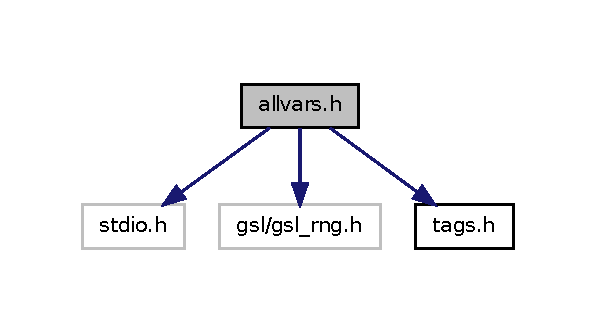
\includegraphics[width=286pt]{allvars_8h__incl}
\end{center}
\end{figure}
This graph shows which files directly or indirectly include this file:
\nopagebreak
\begin{figure}[H]
\begin{center}
\leavevmode
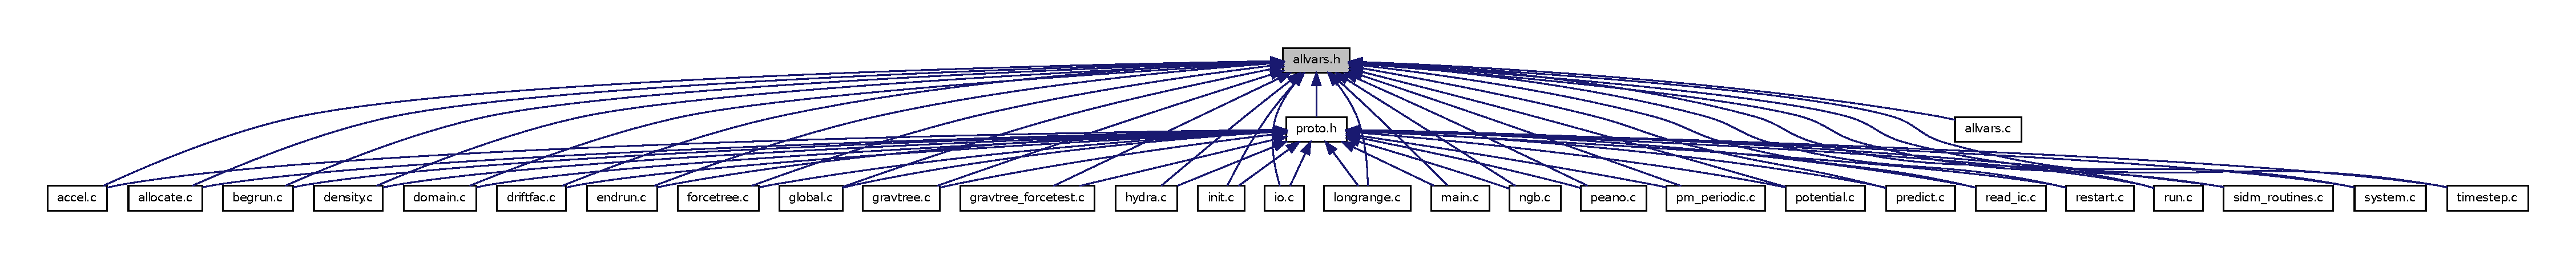
\includegraphics[width=400pt]{allvars_8h__dep__incl}
\end{center}
\end{figure}
\subsection*{Data Structures}
\begin{DoxyCompactItemize}
\item 
struct \hyperlink{structDomainNODE}{DomainNODE}
\item 
struct \hyperlink{structtopnode__data}{topnode\_\-data}
\item 
struct \hyperlink{structglobal__data__all__processes}{global\_\-data\_\-all\_\-processes}
\item 
struct \hyperlink{structparticle__data}{particle\_\-data}
\item 
struct \hyperlink{structsph__particle__data}{sph\_\-particle\_\-data}
\item 
struct \hyperlink{structNODE}{NODE}
\item 
struct \hyperlink{structextNODE}{extNODE}
\item 
struct \hyperlink{structio__header}{io\_\-header}
\item 
struct \hyperlink{structstate__of__system}{state\_\-of\_\-system}
\item 
struct \hyperlink{structgravdata__in}{gravdata\_\-in}
\item 
struct \hyperlink{structgravdata__index}{gravdata\_\-index}
\item 
struct \hyperlink{structdensdata__in}{densdata\_\-in}
\item 
struct \hyperlink{structdensdata__out}{densdata\_\-out}
\item 
struct \hyperlink{structhydrodata__in}{hydrodata\_\-in}
\item 
struct \hyperlink{structhydrodata__out}{hydrodata\_\-out}
\end{DoxyCompactItemize}
\subsection*{Defines}
\begin{DoxyCompactItemize}
\item 
\#define \hyperlink{allvars_8h_aa7cd216e76b2710261f7eb5e862073a7}{GADGETVERSION}~\char`\"{}2.0\char`\"{}
\item 
\#define \hyperlink{allvars_8h_ad44dabdb7a0bef8536e2d34a01177d48}{TIMEBASE}~(1$<$$<$28)
\item 
\#define \hyperlink{allvars_8h_a803069f3cb8753ac3db10d5decebfc0d}{MAXTOPNODES}~200000
\item 
\#define \hyperlink{allvars_8h_a84bc981fa6ccfbb15526a6e9da12087a}{BITS\_\-PER\_\-DIMENSION}~18
\item 
\#define \hyperlink{allvars_8h_a2f881456983c1c8ea9e2ddd76a6eda43}{PEANOCELLS}~(((\hyperlink{allvars_8h_a63f10772bd5776dcb4b6301f425e0d26}{peanokey})1)$<$$<$(3$\ast$BITS\_\-PER\_\-DIMENSION))
\item 
\#define \hyperlink{allvars_8h_a48e4756a015aa76380774eb445183e35}{RNDTABLE}~3000
\item 
\#define \hyperlink{allvars_8h_af277b171beccf0e6d25ff992ded5c566}{MAX\_\-REAL\_\-NUMBER}~1e37
\item 
\#define \hyperlink{allvars_8h_ab7fcc6b0ff94d9cbf1549a03bc6947e0}{MIN\_\-REAL\_\-NUMBER}~1e-\/37
\item 
\#define \hyperlink{allvars_8h_a741a07685761406e6bb951c6f8c9979b}{MAXLEN\_\-FILENAME}~100
\item 
\#define \hyperlink{allvars_8h_a8659b9de3e544ff142b153b076f30fd5}{GAMMA}~(5.0/3)
\item 
\#define \hyperlink{allvars_8h_a75216f9bf4030240b1fc0e1855e032d2}{GAMMA\_\-MINUS1}~(GAMMA-\/1)
\item 
\#define \hyperlink{allvars_8h_a67abaa49a5aa2892eba705d380652279}{HYDROGEN\_\-MASSFRAC}~0.76
\item 
\#define \hyperlink{allvars_8h_a6801baa546c6112d19eb095111d24720}{GRAVITY}~6.672e-\/8
\item 
\#define \hyperlink{allvars_8h_a6321c9a4f727494edf637f2c5559af44}{SOLAR\_\-MASS}~1.989e33
\item 
\#define \hyperlink{allvars_8h_ab79f83235ac3f37355ad291721d945af}{SOLAR\_\-LUM}~3.826e33
\item 
\#define \hyperlink{allvars_8h_a33ef0a9657b1e7d8065955f913020f0f}{RAD\_\-CONST}~7.565e-\/15
\item 
\#define \hyperlink{allvars_8h_a29763ca81b8e5a8c64dac560ade56b66}{AVOGADRO}~6.0222e23
\item 
\#define \hyperlink{allvars_8h_aa1487dae81baa2e0a5643e7b571633a0}{BOLTZMANN}~1.3806e-\/16
\item 
\#define \hyperlink{allvars_8h_a29ead6f96bcfe50a677f482ec638be15}{GAS\_\-CONST}~8.31425e7
\item 
\#define \hyperlink{allvars_8h_ac4cf4b2ab929bd23951a8676eeac086b}{C}~2.9979e10
\item 
\#define \hyperlink{allvars_8h_abbf43217eff86526797a20fbcfc928d2}{PLANCK}~6.6262e-\/27
\item 
\#define \hyperlink{allvars_8h_a5a80b30e136f7032873530b2a44e224b}{CM\_\-PER\_\-MPC}~3.085678e24
\item 
\#define \hyperlink{allvars_8h_a7e6cfbe5535ec2470a672abeba3fcd4d}{PROTONMASS}~1.6726e-\/24
\item 
\#define \hyperlink{allvars_8h_a3555a5acf70a637cd45d57d5b03b6a38}{ELECTRONMASS}~9.10953e-\/28
\item 
\#define \hyperlink{allvars_8h_a8bc97ad38b30a4ad622f7ebba5654485}{THOMPSON}~6.65245e-\/25
\item 
\#define \hyperlink{allvars_8h_a2edb0a233d93080620be2443484b704c}{ELECTRONCHARGE}~4.8032e-\/10
\item 
\#define \hyperlink{allvars_8h_a5de72d8762faf787d06d4dd47daeddeb}{HUBBLE}~3.2407789e-\/18
\item 
\#define \hyperlink{allvars_8h_af2bfce8e844bbb3b120263471c6c329e}{SEC\_\-PER\_\-MEGAYEAR}~3.155e13
\item 
\#define \hyperlink{allvars_8h_a8cd8e04105fec7cd442d078c303e46b9}{SEC\_\-PER\_\-YEAR}~3.155e7
\item 
\#define \hyperlink{allvars_8h_afde936c3d6ae18fa09bca0eb4e5c88dd}{ASMTH}~1.25
\item 
\#define \hyperlink{allvars_8h_a1757a8f71b37d9f5a7a8c753d9f9cab1}{RCUT}~4.5
\item 
\#define \hyperlink{allvars_8h_a459bf1b27bb8a17c4496d2783e62161c}{MAX\_\-NGB}~20000
\item 
\#define \hyperlink{allvars_8h_a15241b0cd53f02da974a64ebb05dcc8d}{MAXLEN\_\-OUTPUTLIST}~500
\item 
\#define \hyperlink{allvars_8h_aec9dcf4def3489f6890e20e7d66151c6}{DRIFT\_\-TABLE\_\-LENGTH}~1000
\item 
\#define \hyperlink{allvars_8h_a9e60f3e57fde2b9b1c7fe2eab7334add}{MAXITER}~150
\item 
\#define \hyperlink{allvars_8h_ae8690abbffa85934d64d545920e2b108}{FLOAT}~float
\item 
\#define \hyperlink{allvars_8h_a2e32e163509d0638d5c54046429c00b3}{NUMDIMS}~3
\item 
\#define \hyperlink{allvars_8h_ab5f539f35b0297ef0f6650cf869ce461}{KERNEL\_\-COEFF\_\-1}~2.546479089470
\item 
\#define \hyperlink{allvars_8h_a5d38a374d10a6baf4406b7c65b542056}{KERNEL\_\-COEFF\_\-2}~15.278874536822
\item 
\#define \hyperlink{allvars_8h_a3bb5c97343f773154b21becfa01914c3}{KERNEL\_\-COEFF\_\-3}~45.836623610466
\item 
\#define \hyperlink{allvars_8h_ad7427fba6163f65a77142f2a00d7dad1}{KERNEL\_\-COEFF\_\-4}~30.557749073644
\item 
\#define \hyperlink{allvars_8h_a7840162cc2fd06c919b18817d647b667}{KERNEL\_\-COEFF\_\-5}~5.092958178941
\item 
\#define \hyperlink{allvars_8h_a7b9464063f0137e9da842c10d1b86ed2}{KERNEL\_\-COEFF\_\-6}~(-\/15.278874536822)
\item 
\#define \hyperlink{allvars_8h_a2c92c6993dec8847de1e1621d81818ce}{NORM\_\-COEFF}~4.188790204786
\item 
\#define \hyperlink{allvars_8h_a61b78d4c6ae0a8bb9e19476b3ffb7bfb}{IO\_\-NBLOCKS}~11
\end{DoxyCompactItemize}
\subsection*{Typedefs}
\begin{DoxyCompactItemize}
\item 
typedef long long \hyperlink{allvars_8h_a63f10772bd5776dcb4b6301f425e0d26}{peanokey}
\end{DoxyCompactItemize}
\subsection*{Enumerations}
\begin{DoxyCompactItemize}
\item 
enum \hyperlink{allvars_8h_a3f7452ec51c4f746e7070abd666147d8}{iofields} \{ \par
\hyperlink{allvars_8h_a3f7452ec51c4f746e7070abd666147d8a0207eb67d96fe97fb8158c42af624f8f}{IO\_\-POS}, 
\hyperlink{allvars_8h_a3f7452ec51c4f746e7070abd666147d8aa4c3992546632e0db8015ebe534c0282}{IO\_\-VEL}, 
\hyperlink{allvars_8h_a3f7452ec51c4f746e7070abd666147d8a34f71f128fc699de3792687fd79edf03}{IO\_\-ID}, 
\hyperlink{allvars_8h_a3f7452ec51c4f746e7070abd666147d8a72e1cc8b602ab38f0f3491464ed82063}{IO\_\-MASS}, 
\par
\hyperlink{allvars_8h_a3f7452ec51c4f746e7070abd666147d8a942cbf4dca00cd5260edc905f5976682}{IO\_\-U}, 
\hyperlink{allvars_8h_a3f7452ec51c4f746e7070abd666147d8a8dd43018a3f2d1caed951b249a38b106}{IO\_\-RHO}, 
\hyperlink{allvars_8h_a3f7452ec51c4f746e7070abd666147d8a429c6a7a56e3b53597bd1eb72b87f941}{IO\_\-HSML}, 
\hyperlink{allvars_8h_a3f7452ec51c4f746e7070abd666147d8a27c32f555479567b88ad11dcce803fe9}{IO\_\-POT}, 
\par
\hyperlink{allvars_8h_a3f7452ec51c4f746e7070abd666147d8a6f80f32dfa1c0cde8a71b773f42bb97a}{IO\_\-ACCEL}, 
\hyperlink{allvars_8h_a3f7452ec51c4f746e7070abd666147d8a74d42dcd51f76c1919f44e9f89581457}{IO\_\-DTENTR}, 
\hyperlink{allvars_8h_a3f7452ec51c4f746e7070abd666147d8aac2070d9e6c597be29ae9a4c9acc36da}{IO\_\-TSTP}
 \}
\end{DoxyCompactItemize}
\subsection*{Variables}
\begin{DoxyCompactItemize}
\item 
int \hyperlink{allvars_8h_a52c8c7d2abff436111942e02c5bb466a}{ThisTask}
\item 
int \hyperlink{allvars_8h_a675acdcd149f5993271a1fdc11673b65}{NTask}
\item 
int \hyperlink{allvars_8h_a9a18606803f69f24d3cb2864640c122e}{PTask}
\item 
int \hyperlink{allvars_8h_a9ec69b53278f9bbe12890e50299026af}{NumPart}
\item 
int \hyperlink{allvars_8h_a8312e7470883d71db46cda5f1e616974}{N\_\-gas}
\item 
long long \hyperlink{allvars_8h_a697577a2a59bfa869161211cb134a6ae}{Ntype} \mbox{[}6\mbox{]}
\item 
int \hyperlink{allvars_8h_a7e6cdb6eab38cb043edcf56a4518dfca}{NtypeLocal} \mbox{[}6\mbox{]}
\item 
int \hyperlink{allvars_8h_a4c8b412a9883b4f6e0e8962ba54fd4ef}{NumForceUpdate}
\item 
int \hyperlink{allvars_8h_a0da112f9d57d7d936055dbb1035cd7fa}{NumSphUpdate}
\item 
double \hyperlink{allvars_8h_a2550e86a899b36eaf7428b23f98a05ec}{CPUThisRun}
\item 
int \hyperlink{allvars_8h_a7f2decfd266dfa9b4560409b9e72b4ab}{RestartFlag}
\item 
char $\ast$ \hyperlink{allvars_8h_a768b23818449e1b33a55747cb3cc2025}{Exportflag}
\item 
int $\ast$ \hyperlink{allvars_8h_ade1b96e6772d0d1ccb06bcbec352b5bd}{Ngblist}
\item 
int \hyperlink{allvars_8h_aa32d7269f9baf3ffdbdd509982fca128}{TreeReconstructFlag}
\item 
int \hyperlink{allvars_8h_a6343a9f3619e77c1796309b8deda7f50}{Flag\_\-FullStep}
\item 
gsl\_\-rng $\ast$ \hyperlink{allvars_8h_a4ec93729b85eb5da23dd6ffb23c3702b}{random\_\-generator}
\item 
double \hyperlink{allvars_8h_aa91f67a734086ebfa758994e579c80a9}{RndTable} \mbox{[}3000\mbox{]}
\item 
double \hyperlink{allvars_8h_a55dacf524ba7bbc5210fc68469a05d0f}{DomainCorner} \mbox{[}3\mbox{]}
\item 
double \hyperlink{allvars_8h_ad13aabcbb50307c005ffa0b2edccdaeb}{DomainCenter} \mbox{[}3\mbox{]}
\item 
double \hyperlink{allvars_8h_a3dd9593672bf68f0c36fa3e5451e9265}{DomainLen}
\item 
double \hyperlink{allvars_8h_a4488078cfcc203156f193c43a1d3a2ef}{DomainFac}
\item 
int \hyperlink{allvars_8h_a424b31dae72cd3331485d2fb6490c7ac}{DomainMyStart}
\item 
int \hyperlink{allvars_8h_ad6c1a01f55d5c8b7b642525118acbebe}{DomainMyLast}
\item 
int $\ast$ \hyperlink{allvars_8h_a3c2a7b96fe94b5151d568fe321888d23}{DomainStartList}
\item 
int $\ast$ \hyperlink{allvars_8h_abb42257c117a39d968334cd054c16dcf}{DomainEndList}
\item 
double $\ast$ \hyperlink{allvars_8h_aed1b2c641567602d5935709a6a05b363}{DomainWork}
\item 
int $\ast$ \hyperlink{allvars_8h_a743ddd39e492911973f9acd210df0c7c}{DomainCount}
\item 
int $\ast$ \hyperlink{allvars_8h_acfb9351c127127b0de4a310bf91974e4}{DomainCountSph}
\item 
int $\ast$ \hyperlink{allvars_8h_a6f4a30ea20d1347d14d2e32de91390bb}{DomainTask}
\item 
int $\ast$ \hyperlink{allvars_8h_acd2b211f08f9b7e83da8cb58bf3931a0}{DomainNodeIndex}
\item 
float $\ast$ \hyperlink{allvars_8h_a52e5390127f5298d6639b9399077bfbf}{DomainTreeNodeLen}
\item 
float $\ast$ \hyperlink{allvars_8h_a5a4689ebf26bc52b81819580362ef4dc}{DomainHmax}
\item 
struct \hyperlink{structDomainNODE}{DomainNODE} $\ast$ \hyperlink{allvars_8h_a422cdcf73caef7cc559090cab77839e3}{DomainMoment}
\item 
\hyperlink{allvars_8h_a63f10772bd5776dcb4b6301f425e0d26}{peanokey} $\ast$ \hyperlink{allvars_8h_a6918a0815266193ad242888c455c5886}{DomainKeyBuf}
\item 
\hyperlink{allvars_8h_a63f10772bd5776dcb4b6301f425e0d26}{peanokey} $\ast$ \hyperlink{allvars_8h_a828333e1bfb5cffdb0e67942bbcd6cdb}{Key}
\item 
\hyperlink{allvars_8h_a63f10772bd5776dcb4b6301f425e0d26}{peanokey} $\ast$ \hyperlink{allvars_8h_a8b9ee62bf965346f051e19e013d998b4}{KeySorted}
\item 
int \hyperlink{allvars_8h_a269a1fc2bea249d93115b160fd42ee84}{NTopnodes}
\item 
int \hyperlink{allvars_8h_a820bd6735d7313b9e7a3dcbe6c2f93d4}{NTopleaves}
\item 
struct \hyperlink{structtopnode__data}{topnode\_\-data} $\ast$ \hyperlink{allvars_8h_a49037625c4cfadc0fc7c0d900486ccc4}{TopNodes}
\item 
double \hyperlink{allvars_8h_ae43d9623e3a2c88558e99ecf90948906}{TimeOfLastTreeConstruction}
\item 
char \hyperlink{allvars_8h_aad74b601033a4fe957c6129de6e8406c}{ParameterFile} \mbox{[}100\mbox{]}
\item 
FILE $\ast$ \hyperlink{allvars_8h_af26719ed46b19cc760b7b55c3cb9968c}{FdInfo}
\item 
FILE $\ast$ \hyperlink{allvars_8h_a0230903e40950ac42dbff71dddd12176}{FdEnergy}
\item 
FILE $\ast$ \hyperlink{allvars_8h_a603fc3e63a037dff4463c67aa7a4c91e}{FdTimings}
\item 
FILE $\ast$ \hyperlink{allvars_8h_a889700103f4f515009e98a7d789fd164}{FdCPU}
\item 
FILE $\ast$ \hyperlink{allvars_8h_ae16a08c18946ccba84c72541b51055dd}{FdForceTest}
\item 
double \hyperlink{allvars_8h_a074db1ef4adfe88a5f3b07eac8c1daae}{DriftTable} \mbox{[}1000\mbox{]}
\item 
double \hyperlink{allvars_8h_a38e5d8b595161f074f7fbede3a8fda66}{GravKickTable} \mbox{[}1000\mbox{]}
\item 
double \hyperlink{allvars_8h_a274a5737d1578d54d6f82130e3064771}{HydroKickTable} \mbox{[}1000\mbox{]}
\item 
void $\ast$ \hyperlink{allvars_8h_ab9d6a5a8cf4049ad304ea6d23d8efb09}{CommBuffer}
\item 
struct \hyperlink{structglobal__data__all__processes}{global\_\-data\_\-all\_\-processes} \hyperlink{allvars_8h_ac8b78c0f0374aecf7aec8da076574dd3}{All}
\item 
struct \hyperlink{structparticle__data}{particle\_\-data} $\ast$ \hyperlink{allvars_8h_ac2474070ba8a23d796836d10c5d5f171}{P}
\item 
struct \hyperlink{structparticle__data}{particle\_\-data} $\ast$ \hyperlink{allvars_8h_a333f7897f74be0a8dbbf252242ab6e6d}{DomainPartBuf}
\item 
struct \hyperlink{structsph__particle__data}{sph\_\-particle\_\-data} $\ast$ \hyperlink{allvars_8h_a8a7e4a61647bbfa2ba060e2828c9a071}{SphP}
\item 
struct \hyperlink{structsph__particle__data}{sph\_\-particle\_\-data} $\ast$ \hyperlink{allvars_8h_ae6cc3e9e736680cf5255430ed1ac9b46}{DomainSphBuf}
\item 
int \hyperlink{allvars_8h_aca70a1751175167a36c1c6775a338bee}{MaxNodes}
\item 
int \hyperlink{allvars_8h_acf4151281b98d29aa500c5e56e66741f}{Numnodestree}
\item 
struct \hyperlink{structNODE}{NODE} $\ast$ \hyperlink{allvars_8h_adcab3d35d39a1fab757a93c8370af036}{Nodes\_\-base}
\item 
struct \hyperlink{structNODE}{NODE} $\ast$ \hyperlink{allvars_8h_a064cd3ea05dbc39224d5c4d6d87a51a4}{Nodes}
\item 
int $\ast$ \hyperlink{allvars_8h_ad14ab43f541f9c33cb9222ea018c1365}{Nextnode}
\item 
int $\ast$ \hyperlink{allvars_8h_ae1adfde6b271afd077130a64e6b85766}{Father}
\item 
struct \hyperlink{structextNODE}{extNODE} $\ast$ \hyperlink{allvars_8h_ab88f28f281293c932082c083b5b37c65}{Extnodes\_\-base}
\item 
struct \hyperlink{structextNODE}{extNODE} $\ast$ \hyperlink{allvars_8h_ae10c0a0d592e19b36fcf68b3492c364f}{Extnodes}
\item 
struct \hyperlink{structio__header}{io\_\-header} \hyperlink{allvars_8h_ab32a0614ea7e4791435d61dbb9652e00}{header}
\item 
char \hyperlink{allvars_8h_ab0664df93d97f96270978b84eb6fb80c}{Tab\_\-IO\_\-Labels} \mbox{[}11\mbox{]}\mbox{[}4\mbox{]}
\item 
struct \hyperlink{structstate__of__system}{state\_\-of\_\-system} \hyperlink{allvars_8h_abf8cf148b3694ed9d2ddfa49c2e88ab0}{SysState}
\item 
struct \hyperlink{structgravdata__in}{gravdata\_\-in} $\ast$ \hyperlink{allvars_8h_a0202ec7197196dd7d7fda746465659d7}{GravDataIn}
\item 
struct \hyperlink{structgravdata__in}{gravdata\_\-in} $\ast$ \hyperlink{allvars_8h_a57d0973f01bdcb2fa5d780058aab11c7}{GravDataGet}
\item 
struct \hyperlink{structgravdata__in}{gravdata\_\-in} $\ast$ \hyperlink{allvars_8h_a77de038fc404ee0d679d54a4b783c508}{GravDataResult}
\item 
struct \hyperlink{structgravdata__in}{gravdata\_\-in} $\ast$ \hyperlink{allvars_8h_aa21c5832ee4077e36639e1357252a3c3}{GravDataOut}
\item 
struct \hyperlink{structgravdata__index}{gravdata\_\-index} $\ast$ \hyperlink{allvars_8h_ab5ef88b406ac9d29bbd68978d47bdcde}{GravDataIndexTable}
\item 
struct \hyperlink{structdensdata__in}{densdata\_\-in} $\ast$ \hyperlink{allvars_8h_af36a3314e5ba2993fb9f4bd31f1fb46e}{DensDataIn}
\item 
struct \hyperlink{structdensdata__in}{densdata\_\-in} $\ast$ \hyperlink{allvars_8h_adce7bcb3ba145a70337ac58206404f7a}{DensDataGet}
\item 
struct \hyperlink{structdensdata__out}{densdata\_\-out} $\ast$ \hyperlink{allvars_8h_a9038ccdd06875b04b52dd3e1c1ebf5d8}{DensDataResult}
\item 
struct \hyperlink{structdensdata__out}{densdata\_\-out} $\ast$ \hyperlink{allvars_8h_adf1e42b0c831dc0da9690458a9f4e355}{DensDataPartialResult}
\item 
struct \hyperlink{structhydrodata__in}{hydrodata\_\-in} $\ast$ \hyperlink{allvars_8h_ab0bc3f2f42a5306625ed069dbc8d000a}{HydroDataIn}
\item 
struct \hyperlink{structhydrodata__in}{hydrodata\_\-in} $\ast$ \hyperlink{allvars_8h_a9a89bbf2d5e91c917a65e180b0551db5}{HydroDataGet}
\item 
struct \hyperlink{structhydrodata__out}{hydrodata\_\-out} $\ast$ \hyperlink{allvars_8h_a640e014b66b10adc033a159528455534}{HydroDataResult}
\item 
struct \hyperlink{structhydrodata__out}{hydrodata\_\-out} $\ast$ \hyperlink{allvars_8h_ae2294233324fafb23adc0248a48c5f82}{HydroDataPartialResult}
\end{DoxyCompactItemize}


\subsection{Detailed Description}
declares global variables. This file declares all global variables. Further variables should be added here, and declared as 'extern'. The actual existence of these variables is provided by the file 'allvars.c'. To produce 'allvars.c' from 'allvars.h', do the following:


\begin{DoxyItemize}
\item Erase all define's, typedef's, and enum's
\item add include \char`\"{}allvars.h\char`\"{}, delete the ifndef ALLVARS\_\-H conditional
\item delete all keywords 'extern'
\item delete all struct definitions enclosed in \{...\}, e.g. \char`\"{}extern struct global\_\-data\_\-all\_\-processes \{....\} All;\char`\"{} becomes \char`\"{}struct global\_\-data\_\-all\_\-processes All;\char`\"{} 
\end{DoxyItemize}

Definition in file \hyperlink{allvars_8h_source}{allvars.h}.



\subsection{Define Documentation}
\hypertarget{allvars_8h_afde936c3d6ae18fa09bca0eb4e5c88dd}{
\index{allvars.h@{allvars.h}!ASMTH@{ASMTH}}
\index{ASMTH@{ASMTH}!allvars.h@{allvars.h}}
\subsubsection[{ASMTH}]{\setlength{\rightskip}{0pt plus 5cm}\#define ASMTH~1.25}}
\label{allvars_8h_afde936c3d6ae18fa09bca0eb4e5c88dd}
ASMTH gives the scale of the short-\/range/long-\/range force split in units of FFT-\/mesh cells 

Definition at line 99 of file allvars.h.



Referenced by pm\_\-init\_\-periodic().

\hypertarget{allvars_8h_a29763ca81b8e5a8c64dac560ade56b66}{
\index{allvars.h@{allvars.h}!AVOGADRO@{AVOGADRO}}
\index{AVOGADRO@{AVOGADRO}!allvars.h@{allvars.h}}
\subsubsection[{AVOGADRO}]{\setlength{\rightskip}{0pt plus 5cm}\#define AVOGADRO~6.0222e23}}
\label{allvars_8h_a29763ca81b8e5a8c64dac560ade56b66}


Definition at line 81 of file allvars.h.

\hypertarget{allvars_8h_a84bc981fa6ccfbb15526a6e9da12087a}{
\index{allvars.h@{allvars.h}!BITS\_\-PER\_\-DIMENSION@{BITS\_\-PER\_\-DIMENSION}}
\index{BITS\_\-PER\_\-DIMENSION@{BITS\_\-PER\_\-DIMENSION}!allvars.h@{allvars.h}}
\subsubsection[{BITS\_\-PER\_\-DIMENSION}]{\setlength{\rightskip}{0pt plus 5cm}\#define BITS\_\-PER\_\-DIMENSION~18}}
\label{allvars_8h_a84bc981fa6ccfbb15526a6e9da12087a}
Bits per dimension available for Peano-\/Hilbert order. Note: If peanokey is defined as type int, the allowed maximum is 10. If 64-\/bit integers are used, the maximum is 21 

Definition at line 50 of file allvars.h.



Referenced by domain\_\-determineTopTree(), and force\_\-treebuild\_\-single().

\hypertarget{allvars_8h_aa1487dae81baa2e0a5643e7b571633a0}{
\index{allvars.h@{allvars.h}!BOLTZMANN@{BOLTZMANN}}
\index{BOLTZMANN@{BOLTZMANN}!allvars.h@{allvars.h}}
\subsubsection[{BOLTZMANN}]{\setlength{\rightskip}{0pt plus 5cm}\#define BOLTZMANN~1.3806e-\/16}}
\label{allvars_8h_aa1487dae81baa2e0a5643e7b571633a0}


Definition at line 82 of file allvars.h.



Referenced by read\_\-ic(), and set\_\-units().

\hypertarget{allvars_8h_ac4cf4b2ab929bd23951a8676eeac086b}{
\index{allvars.h@{allvars.h}!C@{C}}
\index{C@{C}!allvars.h@{allvars.h}}
\subsubsection[{C}]{\setlength{\rightskip}{0pt plus 5cm}\#define C~2.9979e10}}
\label{allvars_8h_ac4cf4b2ab929bd23951a8676eeac086b}


Definition at line 84 of file allvars.h.

\hypertarget{allvars_8h_a5a80b30e136f7032873530b2a44e224b}{
\index{allvars.h@{allvars.h}!CM\_\-PER\_\-MPC@{CM\_\-PER\_\-MPC}}
\index{CM\_\-PER\_\-MPC@{CM\_\-PER\_\-MPC}!allvars.h@{allvars.h}}
\subsubsection[{CM\_\-PER\_\-MPC}]{\setlength{\rightskip}{0pt plus 5cm}\#define CM\_\-PER\_\-MPC~3.085678e24}}
\label{allvars_8h_a5a80b30e136f7032873530b2a44e224b}


Definition at line 86 of file allvars.h.

\hypertarget{allvars_8h_aec9dcf4def3489f6890e20e7d66151c6}{
\index{allvars.h@{allvars.h}!DRIFT\_\-TABLE\_\-LENGTH@{DRIFT\_\-TABLE\_\-LENGTH}}
\index{DRIFT\_\-TABLE\_\-LENGTH@{DRIFT\_\-TABLE\_\-LENGTH}!allvars.h@{allvars.h}}
\subsubsection[{DRIFT\_\-TABLE\_\-LENGTH}]{\setlength{\rightskip}{0pt plus 5cm}\#define DRIFT\_\-TABLE\_\-LENGTH~1000}}
\label{allvars_8h_aec9dcf4def3489f6890e20e7d66151c6}
length of the lookup table used to hold the drift and kick factors 

Definition at line 111 of file allvars.h.



Referenced by get\_\-drift\_\-factor(), get\_\-gravkick\_\-factor(), and get\_\-hydrokick\_\-factor().

\hypertarget{allvars_8h_a2edb0a233d93080620be2443484b704c}{
\index{allvars.h@{allvars.h}!ELECTRONCHARGE@{ELECTRONCHARGE}}
\index{ELECTRONCHARGE@{ELECTRONCHARGE}!allvars.h@{allvars.h}}
\subsubsection[{ELECTRONCHARGE}]{\setlength{\rightskip}{0pt plus 5cm}\#define ELECTRONCHARGE~4.8032e-\/10}}
\label{allvars_8h_a2edb0a233d93080620be2443484b704c}


Definition at line 90 of file allvars.h.

\hypertarget{allvars_8h_a3555a5acf70a637cd45d57d5b03b6a38}{
\index{allvars.h@{allvars.h}!ELECTRONMASS@{ELECTRONMASS}}
\index{ELECTRONMASS@{ELECTRONMASS}!allvars.h@{allvars.h}}
\subsubsection[{ELECTRONMASS}]{\setlength{\rightskip}{0pt plus 5cm}\#define ELECTRONMASS~9.10953e-\/28}}
\label{allvars_8h_a3555a5acf70a637cd45d57d5b03b6a38}


Definition at line 88 of file allvars.h.

\hypertarget{allvars_8h_ae8690abbffa85934d64d545920e2b108}{
\index{allvars.h@{allvars.h}!FLOAT@{FLOAT}}
\index{FLOAT@{FLOAT}!allvars.h@{allvars.h}}
\subsubsection[{FLOAT}]{\setlength{\rightskip}{0pt plus 5cm}\#define FLOAT~float}}
\label{allvars_8h_ae8690abbffa85934d64d545920e2b108}


Definition at line 119 of file allvars.h.



Referenced by advance\_\-and\_\-find\_\-timesteps(), allocate\_\-commbuffers(), density\_\-evaluate(), dump\_\-particles(), ewald\_\-init(), fill\_\-write\_\-buffer(), force\_\-treeevaluate(), force\_\-treeevaluate\_\-shortrange(), force\_\-treeupdate\_\-pseudos(), force\_\-update\_\-hmax(), force\_\-update\_\-len(), force\_\-update\_\-node\_\-len\_\-local(), force\_\-update\_\-node\_\-len\_\-toptree(), force\_\-update\_\-node\_\-recursive(), hydro\_\-evaluate(), ngb\_\-clear\_\-buf(), ngb\_\-treefind\_\-pairs(), ngb\_\-treefind\_\-variable(), and restart().

\hypertarget{allvars_8h_aa7cd216e76b2710261f7eb5e862073a7}{
\index{allvars.h@{allvars.h}!GADGETVERSION@{GADGETVERSION}}
\index{GADGETVERSION@{GADGETVERSION}!allvars.h@{allvars.h}}
\subsubsection[{GADGETVERSION}]{\setlength{\rightskip}{0pt plus 5cm}\#define GADGETVERSION~\char`\"{}2.0\char`\"{}}}
\label{allvars_8h_aa7cd216e76b2710261f7eb5e862073a7}
code version string 

Definition at line 39 of file allvars.h.



Referenced by begrun().

\hypertarget{allvars_8h_a8659b9de3e544ff142b153b076f30fd5}{
\index{allvars.h@{allvars.h}!GAMMA@{GAMMA}}
\index{GAMMA@{GAMMA}!allvars.h@{allvars.h}}
\subsubsection[{GAMMA}]{\setlength{\rightskip}{0pt plus 5cm}\#define GAMMA~(5.0/3)}}
\label{allvars_8h_a8659b9de3e544ff142b153b076f30fd5}
adiabatic index of simulated gas 

Definition at line 68 of file allvars.h.



Referenced by advance\_\-and\_\-find\_\-timesteps(), density(), fill\_\-write\_\-buffer(), get\_\-timestep(), hydro\_\-evaluate(), hydro\_\-force(), and move\_\-particles().

\hypertarget{allvars_8h_a75216f9bf4030240b1fc0e1855e032d2}{
\index{allvars.h@{allvars.h}!GAMMA\_\-MINUS1@{GAMMA\_\-MINUS1}}
\index{GAMMA\_\-MINUS1@{GAMMA\_\-MINUS1}!allvars.h@{allvars.h}}
\subsubsection[{GAMMA\_\-MINUS1}]{\setlength{\rightskip}{0pt plus 5cm}\#define GAMMA\_\-MINUS1~(GAMMA-\/1)}}
\label{allvars_8h_a75216f9bf4030240b1fc0e1855e032d2}


Definition at line 71 of file allvars.h.



Referenced by advance\_\-and\_\-find\_\-timesteps(), compute\_\-global\_\-quantities\_\-of\_\-system(), fill\_\-write\_\-buffer(), hydro\_\-force(), hydrokick\_\-integ(), init(), and read\_\-ic().

\hypertarget{allvars_8h_a29ead6f96bcfe50a677f482ec638be15}{
\index{allvars.h@{allvars.h}!GAS\_\-CONST@{GAS\_\-CONST}}
\index{GAS\_\-CONST@{GAS\_\-CONST}!allvars.h@{allvars.h}}
\subsubsection[{GAS\_\-CONST}]{\setlength{\rightskip}{0pt plus 5cm}\#define GAS\_\-CONST~8.31425e7}}
\label{allvars_8h_a29ead6f96bcfe50a677f482ec638be15}


Definition at line 83 of file allvars.h.

\hypertarget{allvars_8h_a6801baa546c6112d19eb095111d24720}{
\index{allvars.h@{allvars.h}!GRAVITY@{GRAVITY}}
\index{GRAVITY@{GRAVITY}!allvars.h@{allvars.h}}
\subsubsection[{GRAVITY}]{\setlength{\rightskip}{0pt plus 5cm}\#define GRAVITY~6.672e-\/8}}
\label{allvars_8h_a6801baa546c6112d19eb095111d24720}
Gravitational constant (in cgs units) 

Definition at line 77 of file allvars.h.



Referenced by set\_\-units().

\hypertarget{allvars_8h_a5de72d8762faf787d06d4dd47daeddeb}{
\index{allvars.h@{allvars.h}!HUBBLE@{HUBBLE}}
\index{HUBBLE@{HUBBLE}!allvars.h@{allvars.h}}
\subsubsection[{HUBBLE}]{\setlength{\rightskip}{0pt plus 5cm}\#define HUBBLE~3.2407789e-\/18}}
\label{allvars_8h_a5de72d8762faf787d06d4dd47daeddeb}


Definition at line 91 of file allvars.h.



Referenced by set\_\-units().

\hypertarget{allvars_8h_a67abaa49a5aa2892eba705d380652279}{
\index{allvars.h@{allvars.h}!HYDROGEN\_\-MASSFRAC@{HYDROGEN\_\-MASSFRAC}}
\index{HYDROGEN\_\-MASSFRAC@{HYDROGEN\_\-MASSFRAC}!allvars.h@{allvars.h}}
\subsubsection[{HYDROGEN\_\-MASSFRAC}]{\setlength{\rightskip}{0pt plus 5cm}\#define HYDROGEN\_\-MASSFRAC~0.76}}
\label{allvars_8h_a67abaa49a5aa2892eba705d380652279}
mass fraction of hydrogen, relevant only for radiative cooling 

Definition at line 73 of file allvars.h.

\hypertarget{allvars_8h_a61b78d4c6ae0a8bb9e19476b3ffb7bfb}{
\index{allvars.h@{allvars.h}!IO\_\-NBLOCKS@{IO\_\-NBLOCKS}}
\index{IO\_\-NBLOCKS@{IO\_\-NBLOCKS}!allvars.h@{allvars.h}}
\subsubsection[{IO\_\-NBLOCKS}]{\setlength{\rightskip}{0pt plus 5cm}\#define IO\_\-NBLOCKS~11}}
\label{allvars_8h_a61b78d4c6ae0a8bb9e19476b3ffb7bfb}
total number of defined information blocks for snapshot files. Must be equal to the number of entries in \char`\"{}enum iofields\char`\"{} 

Definition at line 656 of file allvars.h.

\hypertarget{allvars_8h_ab5f539f35b0297ef0f6650cf869ce461}{
\index{allvars.h@{allvars.h}!KERNEL\_\-COEFF\_\-1@{KERNEL\_\-COEFF\_\-1}}
\index{KERNEL\_\-COEFF\_\-1@{KERNEL\_\-COEFF\_\-1}!allvars.h@{allvars.h}}
\subsubsection[{KERNEL\_\-COEFF\_\-1}]{\setlength{\rightskip}{0pt plus 5cm}\#define KERNEL\_\-COEFF\_\-1~2.546479089470}}
\label{allvars_8h_ab5f539f35b0297ef0f6650cf869ce461}
Coefficients for SPH spline kernel and its derivative 

Definition at line 125 of file allvars.h.



Referenced by density\_\-evaluate(), and kernel().

\hypertarget{allvars_8h_a5d38a374d10a6baf4406b7c65b542056}{
\index{allvars.h@{allvars.h}!KERNEL\_\-COEFF\_\-2@{KERNEL\_\-COEFF\_\-2}}
\index{KERNEL\_\-COEFF\_\-2@{KERNEL\_\-COEFF\_\-2}!allvars.h@{allvars.h}}
\subsubsection[{KERNEL\_\-COEFF\_\-2}]{\setlength{\rightskip}{0pt plus 5cm}\#define KERNEL\_\-COEFF\_\-2~15.278874536822}}
\label{allvars_8h_a5d38a374d10a6baf4406b7c65b542056}


Definition at line 126 of file allvars.h.



Referenced by density\_\-evaluate(), and kernel().

\hypertarget{allvars_8h_a3bb5c97343f773154b21becfa01914c3}{
\index{allvars.h@{allvars.h}!KERNEL\_\-COEFF\_\-3@{KERNEL\_\-COEFF\_\-3}}
\index{KERNEL\_\-COEFF\_\-3@{KERNEL\_\-COEFF\_\-3}!allvars.h@{allvars.h}}
\subsubsection[{KERNEL\_\-COEFF\_\-3}]{\setlength{\rightskip}{0pt plus 5cm}\#define KERNEL\_\-COEFF\_\-3~45.836623610466}}
\label{allvars_8h_a3bb5c97343f773154b21becfa01914c3}


Definition at line 127 of file allvars.h.



Referenced by density\_\-evaluate(), and hydro\_\-evaluate().

\hypertarget{allvars_8h_ad7427fba6163f65a77142f2a00d7dad1}{
\index{allvars.h@{allvars.h}!KERNEL\_\-COEFF\_\-4@{KERNEL\_\-COEFF\_\-4}}
\index{KERNEL\_\-COEFF\_\-4@{KERNEL\_\-COEFF\_\-4}!allvars.h@{allvars.h}}
\subsubsection[{KERNEL\_\-COEFF\_\-4}]{\setlength{\rightskip}{0pt plus 5cm}\#define KERNEL\_\-COEFF\_\-4~30.557749073644}}
\label{allvars_8h_ad7427fba6163f65a77142f2a00d7dad1}


Definition at line 128 of file allvars.h.

\hypertarget{allvars_8h_a7840162cc2fd06c919b18817d647b667}{
\index{allvars.h@{allvars.h}!KERNEL\_\-COEFF\_\-5@{KERNEL\_\-COEFF\_\-5}}
\index{KERNEL\_\-COEFF\_\-5@{KERNEL\_\-COEFF\_\-5}!allvars.h@{allvars.h}}
\subsubsection[{KERNEL\_\-COEFF\_\-5}]{\setlength{\rightskip}{0pt plus 5cm}\#define KERNEL\_\-COEFF\_\-5~5.092958178941}}
\label{allvars_8h_a7840162cc2fd06c919b18817d647b667}


Definition at line 129 of file allvars.h.



Referenced by density\_\-evaluate(), and kernel().

\hypertarget{allvars_8h_a7b9464063f0137e9da842c10d1b86ed2}{
\index{allvars.h@{allvars.h}!KERNEL\_\-COEFF\_\-6@{KERNEL\_\-COEFF\_\-6}}
\index{KERNEL\_\-COEFF\_\-6@{KERNEL\_\-COEFF\_\-6}!allvars.h@{allvars.h}}
\subsubsection[{KERNEL\_\-COEFF\_\-6}]{\setlength{\rightskip}{0pt plus 5cm}\#define KERNEL\_\-COEFF\_\-6~(-\/15.278874536822)}}
\label{allvars_8h_a7b9464063f0137e9da842c10d1b86ed2}


Definition at line 130 of file allvars.h.



Referenced by density\_\-evaluate(), and hydro\_\-evaluate().

\hypertarget{allvars_8h_a459bf1b27bb8a17c4496d2783e62161c}{
\index{allvars.h@{allvars.h}!MAX\_\-NGB@{MAX\_\-NGB}}
\index{MAX\_\-NGB@{MAX\_\-NGB}!allvars.h@{allvars.h}}
\subsubsection[{MAX\_\-NGB}]{\setlength{\rightskip}{0pt plus 5cm}\#define MAX\_\-NGB~20000}}
\label{allvars_8h_a459bf1b27bb8a17c4496d2783e62161c}
defines maximum length of neighbour list 

Definition at line 107 of file allvars.h.



Referenced by init(), ngb\_\-treefind\_\-pairs(), ngb\_\-treefind\_\-variable(), and restart().

\hypertarget{allvars_8h_af277b171beccf0e6d25ff992ded5c566}{
\index{allvars.h@{allvars.h}!MAX\_\-REAL\_\-NUMBER@{MAX\_\-REAL\_\-NUMBER}}
\index{MAX\_\-REAL\_\-NUMBER@{MAX\_\-REAL\_\-NUMBER}!allvars.h@{allvars.h}}
\subsubsection[{MAX\_\-REAL\_\-NUMBER}]{\setlength{\rightskip}{0pt plus 5cm}\#define MAX\_\-REAL\_\-NUMBER~1e37}}
\label{allvars_8h_af277b171beccf0e6d25ff992ded5c566}


Definition at line 60 of file allvars.h.

\hypertarget{allvars_8h_a9e60f3e57fde2b9b1c7fe2eab7334add}{
\index{allvars.h@{allvars.h}!MAXITER@{MAXITER}}
\index{MAXITER@{MAXITER}!allvars.h@{allvars.h}}
\subsubsection[{MAXITER}]{\setlength{\rightskip}{0pt plus 5cm}\#define MAXITER~150}}
\label{allvars_8h_a9e60f3e57fde2b9b1c7fe2eab7334add}
maxmimum number of steps for SPH neighbour iteration If defined, the variable type FLOAT is set to \char`\"{}double\char`\"{}, otherwise to FLOAT 

Definition at line 113 of file allvars.h.



Referenced by density().

\hypertarget{allvars_8h_a741a07685761406e6bb951c6f8c9979b}{
\index{allvars.h@{allvars.h}!MAXLEN\_\-FILENAME@{MAXLEN\_\-FILENAME}}
\index{MAXLEN\_\-FILENAME@{MAXLEN\_\-FILENAME}!allvars.h@{allvars.h}}
\subsubsection[{MAXLEN\_\-FILENAME}]{\setlength{\rightskip}{0pt plus 5cm}\#define MAXLEN\_\-FILENAME~100}}
\label{allvars_8h_a741a07685761406e6bb951c6f8c9979b}
Maximum number of characters for filenames (including the full path) 

Definition at line 63 of file allvars.h.

\hypertarget{allvars_8h_a15241b0cd53f02da974a64ebb05dcc8d}{
\index{allvars.h@{allvars.h}!MAXLEN\_\-OUTPUTLIST@{MAXLEN\_\-OUTPUTLIST}}
\index{MAXLEN\_\-OUTPUTLIST@{MAXLEN\_\-OUTPUTLIST}!allvars.h@{allvars.h}}
\subsubsection[{MAXLEN\_\-OUTPUTLIST}]{\setlength{\rightskip}{0pt plus 5cm}\#define MAXLEN\_\-OUTPUTLIST~500}}
\label{allvars_8h_a15241b0cd53f02da974a64ebb05dcc8d}
maxmimum number of entries in list of snapshot output times 

Definition at line 109 of file allvars.h.



Referenced by read\_\-outputlist().

\hypertarget{allvars_8h_a803069f3cb8753ac3db10d5decebfc0d}{
\index{allvars.h@{allvars.h}!MAXTOPNODES@{MAXTOPNODES}}
\index{MAXTOPNODES@{MAXTOPNODES}!allvars.h@{allvars.h}}
\subsubsection[{MAXTOPNODES}]{\setlength{\rightskip}{0pt plus 5cm}\#define MAXTOPNODES~200000}}
\label{allvars_8h_a803069f3cb8753ac3db10d5decebfc0d}
Maximum number of nodes in the top-\/level tree used for domain decomposition 

Definition at line 45 of file allvars.h.



Referenced by allocate\_\-commbuffers(), domain\_\-topsplit(), domain\_\-topsplit\_\-local(), force\_\-treeallocate(), and restart().

\hypertarget{allvars_8h_ab7fcc6b0ff94d9cbf1549a03bc6947e0}{
\index{allvars.h@{allvars.h}!MIN\_\-REAL\_\-NUMBER@{MIN\_\-REAL\_\-NUMBER}}
\index{MIN\_\-REAL\_\-NUMBER@{MIN\_\-REAL\_\-NUMBER}!allvars.h@{allvars.h}}
\subsubsection[{MIN\_\-REAL\_\-NUMBER}]{\setlength{\rightskip}{0pt plus 5cm}\#define MIN\_\-REAL\_\-NUMBER~1e-\/37}}
\label{allvars_8h_ab7fcc6b0ff94d9cbf1549a03bc6947e0}


Definition at line 61 of file allvars.h.

\hypertarget{allvars_8h_a2c92c6993dec8847de1e1621d81818ce}{
\index{allvars.h@{allvars.h}!NORM\_\-COEFF@{NORM\_\-COEFF}}
\index{NORM\_\-COEFF@{NORM\_\-COEFF}!allvars.h@{allvars.h}}
\subsubsection[{NORM\_\-COEFF}]{\setlength{\rightskip}{0pt plus 5cm}\#define NORM\_\-COEFF~4.188790204786}}
\label{allvars_8h_a2c92c6993dec8847de1e1621d81818ce}
Coefficient for kernel normalization. Note: 4.0/3 $\ast$ PI = 4.188790204786 

Definition at line 131 of file allvars.h.



Referenced by density\_\-evaluate().

\hypertarget{allvars_8h_a2e32e163509d0638d5c54046429c00b3}{
\index{allvars.h@{allvars.h}!NUMDIMS@{NUMDIMS}}
\index{NUMDIMS@{NUMDIMS}!allvars.h@{allvars.h}}
\subsubsection[{NUMDIMS}]{\setlength{\rightskip}{0pt plus 5cm}\#define NUMDIMS~3}}
\label{allvars_8h_a2e32e163509d0638d5c54046429c00b3}
For 3D-\/normalized kernel 

Definition at line 124 of file allvars.h.



Referenced by density(), and density\_\-evaluate().

\hypertarget{allvars_8h_a2f881456983c1c8ea9e2ddd76a6eda43}{
\index{allvars.h@{allvars.h}!PEANOCELLS@{PEANOCELLS}}
\index{PEANOCELLS@{PEANOCELLS}!allvars.h@{allvars.h}}
\subsubsection[{PEANOCELLS}]{\setlength{\rightskip}{0pt plus 5cm}\#define PEANOCELLS~((({\bf peanokey})1)$<$$<$(3$\ast$BITS\_\-PER\_\-DIMENSION))}}
\label{allvars_8h_a2f881456983c1c8ea9e2ddd76a6eda43}
The number of different Peano-\/Hilbert cells 

Definition at line 54 of file allvars.h.

\hypertarget{allvars_8h_abbf43217eff86526797a20fbcfc928d2}{
\index{allvars.h@{allvars.h}!PLANCK@{PLANCK}}
\index{PLANCK@{PLANCK}!allvars.h@{allvars.h}}
\subsubsection[{PLANCK}]{\setlength{\rightskip}{0pt plus 5cm}\#define PLANCK~6.6262e-\/27}}
\label{allvars_8h_abbf43217eff86526797a20fbcfc928d2}


Definition at line 85 of file allvars.h.

\hypertarget{allvars_8h_a7e6cfbe5535ec2470a672abeba3fcd4d}{
\index{allvars.h@{allvars.h}!PROTONMASS@{PROTONMASS}}
\index{PROTONMASS@{PROTONMASS}!allvars.h@{allvars.h}}
\subsubsection[{PROTONMASS}]{\setlength{\rightskip}{0pt plus 5cm}\#define PROTONMASS~1.6726e-\/24}}
\label{allvars_8h_a7e6cfbe5535ec2470a672abeba3fcd4d}


Definition at line 87 of file allvars.h.



Referenced by set\_\-units().

\hypertarget{allvars_8h_a33ef0a9657b1e7d8065955f913020f0f}{
\index{allvars.h@{allvars.h}!RAD\_\-CONST@{RAD\_\-CONST}}
\index{RAD\_\-CONST@{RAD\_\-CONST}!allvars.h@{allvars.h}}
\subsubsection[{RAD\_\-CONST}]{\setlength{\rightskip}{0pt plus 5cm}\#define RAD\_\-CONST~7.565e-\/15}}
\label{allvars_8h_a33ef0a9657b1e7d8065955f913020f0f}


Definition at line 80 of file allvars.h.

\hypertarget{allvars_8h_a1757a8f71b37d9f5a7a8c753d9f9cab1}{
\index{allvars.h@{allvars.h}!RCUT@{RCUT}}
\index{RCUT@{RCUT}!allvars.h@{allvars.h}}
\subsubsection[{RCUT}]{\setlength{\rightskip}{0pt plus 5cm}\#define RCUT~4.5}}
\label{allvars_8h_a1757a8f71b37d9f5a7a8c753d9f9cab1}
RCUT gives the maximum distance (in units of the scale used for the force split) out to which short-\/range forces are evaluated in the short-\/range tree walk. 

Definition at line 103 of file allvars.h.



Referenced by pm\_\-init\_\-periodic().

\hypertarget{allvars_8h_a48e4756a015aa76380774eb445183e35}{
\index{allvars.h@{allvars.h}!RNDTABLE@{RNDTABLE}}
\index{RNDTABLE@{RNDTABLE}!allvars.h@{allvars.h}}
\subsubsection[{RNDTABLE}]{\setlength{\rightskip}{0pt plus 5cm}\#define RNDTABLE~3000}}
\label{allvars_8h_a48e4756a015aa76380774eb445183e35}
gives the length of a table with random numbers, refreshed at every timestep. This is used to allow application of random numbers to a specific particle in a way that is independent of the number of processors used. 

Definition at line 57 of file allvars.h.

\hypertarget{allvars_8h_af2bfce8e844bbb3b120263471c6c329e}{
\index{allvars.h@{allvars.h}!SEC\_\-PER\_\-MEGAYEAR@{SEC\_\-PER\_\-MEGAYEAR}}
\index{SEC\_\-PER\_\-MEGAYEAR@{SEC\_\-PER\_\-MEGAYEAR}!allvars.h@{allvars.h}}
\subsubsection[{SEC\_\-PER\_\-MEGAYEAR}]{\setlength{\rightskip}{0pt plus 5cm}\#define SEC\_\-PER\_\-MEGAYEAR~3.155e13}}
\label{allvars_8h_af2bfce8e844bbb3b120263471c6c329e}


Definition at line 95 of file allvars.h.

\hypertarget{allvars_8h_a8cd8e04105fec7cd442d078c303e46b9}{
\index{allvars.h@{allvars.h}!SEC\_\-PER\_\-YEAR@{SEC\_\-PER\_\-YEAR}}
\index{SEC\_\-PER\_\-YEAR@{SEC\_\-PER\_\-YEAR}!allvars.h@{allvars.h}}
\subsubsection[{SEC\_\-PER\_\-YEAR}]{\setlength{\rightskip}{0pt plus 5cm}\#define SEC\_\-PER\_\-YEAR~3.155e7}}
\label{allvars_8h_a8cd8e04105fec7cd442d078c303e46b9}


Definition at line 96 of file allvars.h.

\hypertarget{allvars_8h_ab79f83235ac3f37355ad291721d945af}{
\index{allvars.h@{allvars.h}!SOLAR\_\-LUM@{SOLAR\_\-LUM}}
\index{SOLAR\_\-LUM@{SOLAR\_\-LUM}!allvars.h@{allvars.h}}
\subsubsection[{SOLAR\_\-LUM}]{\setlength{\rightskip}{0pt plus 5cm}\#define SOLAR\_\-LUM~3.826e33}}
\label{allvars_8h_ab79f83235ac3f37355ad291721d945af}


Definition at line 79 of file allvars.h.

\hypertarget{allvars_8h_a6321c9a4f727494edf637f2c5559af44}{
\index{allvars.h@{allvars.h}!SOLAR\_\-MASS@{SOLAR\_\-MASS}}
\index{SOLAR\_\-MASS@{SOLAR\_\-MASS}!allvars.h@{allvars.h}}
\subsubsection[{SOLAR\_\-MASS}]{\setlength{\rightskip}{0pt plus 5cm}\#define SOLAR\_\-MASS~1.989e33}}
\label{allvars_8h_a6321c9a4f727494edf637f2c5559af44}


Definition at line 78 of file allvars.h.

\hypertarget{allvars_8h_a8bc97ad38b30a4ad622f7ebba5654485}{
\index{allvars.h@{allvars.h}!THOMPSON@{THOMPSON}}
\index{THOMPSON@{THOMPSON}!allvars.h@{allvars.h}}
\subsubsection[{THOMPSON}]{\setlength{\rightskip}{0pt plus 5cm}\#define THOMPSON~6.65245e-\/25}}
\label{allvars_8h_a8bc97ad38b30a4ad622f7ebba5654485}


Definition at line 89 of file allvars.h.

\hypertarget{allvars_8h_ad44dabdb7a0bef8536e2d34a01177d48}{
\index{allvars.h@{allvars.h}!TIMEBASE@{TIMEBASE}}
\index{TIMEBASE@{TIMEBASE}!allvars.h@{allvars.h}}
\subsubsection[{TIMEBASE}]{\setlength{\rightskip}{0pt plus 5cm}\#define TIMEBASE~(1$<$$<$28)}}
\label{allvars_8h_ad44dabdb7a0bef8536e2d34a01177d48}
The simulated timespan is mapped onto the integer interval \mbox{[}0,TIMESPAN\mbox{]}, where TIMESPAN needs to be a power of 2. Note that (1$<$$<$28) corresponds to 2$^\wedge$29 

Definition at line 41 of file allvars.h.



Referenced by advance\_\-and\_\-find\_\-timesteps(), get\_\-timestep(), init(), readjust\_\-timebase(), and run().



\subsection{Typedef Documentation}
\hypertarget{allvars_8h_a63f10772bd5776dcb4b6301f425e0d26}{
\index{allvars.h@{allvars.h}!peanokey@{peanokey}}
\index{peanokey@{peanokey}!allvars.h@{allvars.h}}
\subsubsection[{peanokey}]{\setlength{\rightskip}{0pt plus 5cm}typedef long long {\bf peanokey}}}
\label{allvars_8h_a63f10772bd5776dcb4b6301f425e0d26}
defines the variable type used for Peano-\/Hilbert keys 

Definition at line 48 of file allvars.h.



\subsection{Enumeration Type Documentation}
\hypertarget{allvars_8h_a3f7452ec51c4f746e7070abd666147d8}{
\index{allvars.h@{allvars.h}!iofields@{iofields}}
\index{iofields@{iofields}!allvars.h@{allvars.h}}
\subsubsection[{iofields}]{\setlength{\rightskip}{0pt plus 5cm}enum {\bf iofields}}}
\label{allvars_8h_a3f7452ec51c4f746e7070abd666147d8}
$<$ this enumeration lists the defined output blocks in snapshot files. Not all of them need to be present. \begin{Desc}
\item[Enumerator: ]\par
\begin{description}
\index{IO\_\-POS@{IO\_\-POS}!allvars.h@{allvars.h}}\index{allvars.h@{allvars.h}!IO\_\-POS@{IO\_\-POS}}\item[{\em 
\hypertarget{allvars_8h_a3f7452ec51c4f746e7070abd666147d8a0207eb67d96fe97fb8158c42af624f8f}{
IO\_\-POS}
\label{allvars_8h_a3f7452ec51c4f746e7070abd666147d8a0207eb67d96fe97fb8158c42af624f8f}
}]\index{IO\_\-VEL@{IO\_\-VEL}!allvars.h@{allvars.h}}\index{allvars.h@{allvars.h}!IO\_\-VEL@{IO\_\-VEL}}\item[{\em 
\hypertarget{allvars_8h_a3f7452ec51c4f746e7070abd666147d8aa4c3992546632e0db8015ebe534c0282}{
IO\_\-VEL}
\label{allvars_8h_a3f7452ec51c4f746e7070abd666147d8aa4c3992546632e0db8015ebe534c0282}
}]\index{IO\_\-ID@{IO\_\-ID}!allvars.h@{allvars.h}}\index{allvars.h@{allvars.h}!IO\_\-ID@{IO\_\-ID}}\item[{\em 
\hypertarget{allvars_8h_a3f7452ec51c4f746e7070abd666147d8a34f71f128fc699de3792687fd79edf03}{
IO\_\-ID}
\label{allvars_8h_a3f7452ec51c4f746e7070abd666147d8a34f71f128fc699de3792687fd79edf03}
}]\index{IO\_\-MASS@{IO\_\-MASS}!allvars.h@{allvars.h}}\index{allvars.h@{allvars.h}!IO\_\-MASS@{IO\_\-MASS}}\item[{\em 
\hypertarget{allvars_8h_a3f7452ec51c4f746e7070abd666147d8a72e1cc8b602ab38f0f3491464ed82063}{
IO\_\-MASS}
\label{allvars_8h_a3f7452ec51c4f746e7070abd666147d8a72e1cc8b602ab38f0f3491464ed82063}
}]\index{IO\_\-U@{IO\_\-U}!allvars.h@{allvars.h}}\index{allvars.h@{allvars.h}!IO\_\-U@{IO\_\-U}}\item[{\em 
\hypertarget{allvars_8h_a3f7452ec51c4f746e7070abd666147d8a942cbf4dca00cd5260edc905f5976682}{
IO\_\-U}
\label{allvars_8h_a3f7452ec51c4f746e7070abd666147d8a942cbf4dca00cd5260edc905f5976682}
}]\index{IO\_\-RHO@{IO\_\-RHO}!allvars.h@{allvars.h}}\index{allvars.h@{allvars.h}!IO\_\-RHO@{IO\_\-RHO}}\item[{\em 
\hypertarget{allvars_8h_a3f7452ec51c4f746e7070abd666147d8a8dd43018a3f2d1caed951b249a38b106}{
IO\_\-RHO}
\label{allvars_8h_a3f7452ec51c4f746e7070abd666147d8a8dd43018a3f2d1caed951b249a38b106}
}]\index{IO\_\-HSML@{IO\_\-HSML}!allvars.h@{allvars.h}}\index{allvars.h@{allvars.h}!IO\_\-HSML@{IO\_\-HSML}}\item[{\em 
\hypertarget{allvars_8h_a3f7452ec51c4f746e7070abd666147d8a429c6a7a56e3b53597bd1eb72b87f941}{
IO\_\-HSML}
\label{allvars_8h_a3f7452ec51c4f746e7070abd666147d8a429c6a7a56e3b53597bd1eb72b87f941}
}]\index{IO\_\-POT@{IO\_\-POT}!allvars.h@{allvars.h}}\index{allvars.h@{allvars.h}!IO\_\-POT@{IO\_\-POT}}\item[{\em 
\hypertarget{allvars_8h_a3f7452ec51c4f746e7070abd666147d8a27c32f555479567b88ad11dcce803fe9}{
IO\_\-POT}
\label{allvars_8h_a3f7452ec51c4f746e7070abd666147d8a27c32f555479567b88ad11dcce803fe9}
}]\index{IO\_\-ACCEL@{IO\_\-ACCEL}!allvars.h@{allvars.h}}\index{allvars.h@{allvars.h}!IO\_\-ACCEL@{IO\_\-ACCEL}}\item[{\em 
\hypertarget{allvars_8h_a3f7452ec51c4f746e7070abd666147d8a6f80f32dfa1c0cde8a71b773f42bb97a}{
IO\_\-ACCEL}
\label{allvars_8h_a3f7452ec51c4f746e7070abd666147d8a6f80f32dfa1c0cde8a71b773f42bb97a}
}]\index{IO\_\-DTENTR@{IO\_\-DTENTR}!allvars.h@{allvars.h}}\index{allvars.h@{allvars.h}!IO\_\-DTENTR@{IO\_\-DTENTR}}\item[{\em 
\hypertarget{allvars_8h_a3f7452ec51c4f746e7070abd666147d8a74d42dcd51f76c1919f44e9f89581457}{
IO\_\-DTENTR}
\label{allvars_8h_a3f7452ec51c4f746e7070abd666147d8a74d42dcd51f76c1919f44e9f89581457}
}]\index{IO\_\-TSTP@{IO\_\-TSTP}!allvars.h@{allvars.h}}\index{allvars.h@{allvars.h}!IO\_\-TSTP@{IO\_\-TSTP}}\item[{\em 
\hypertarget{allvars_8h_a3f7452ec51c4f746e7070abd666147d8aac2070d9e6c597be29ae9a4c9acc36da}{
IO\_\-TSTP}
\label{allvars_8h_a3f7452ec51c4f746e7070abd666147d8aac2070d9e6c597be29ae9a4c9acc36da}
}]\end{description}
\end{Desc}



Definition at line 659 of file allvars.h.




\begin{DoxyCode}
{ 
  IO_POS,
  IO_VEL,
  IO_ID,
  IO_MASS,
  IO_U,
  IO_RHO,
  IO_HSML,
  IO_POT,
  IO_ACCEL,
  IO_DTENTR,
  IO_TSTP,
};
\end{DoxyCode}




\subsection{Variable Documentation}
\hypertarget{allvars_8h_ac8b78c0f0374aecf7aec8da076574dd3}{
\index{allvars.h@{allvars.h}!All@{All}}
\index{All@{All}!allvars.h@{allvars.h}}
\subsubsection[{All}]{\setlength{\rightskip}{0pt plus 5cm}struct {\bf global\_\-data\_\-all\_\-processes}
  {\bf All}}}
\label{allvars_8h_ac8b78c0f0374aecf7aec8da076574dd3}
This structure contains data which is the SAME for all tasks (mostly code parameters read from the parameter file). Holding this data in a structure is convenient for writing/reading the restart file, and it allows the introduction of new global variables in a simple way. The only thing to do is to introduce them into this structure. a container variable for global variables that are equal on all processors \hypertarget{allvars_8h_ab9d6a5a8cf4049ad304ea6d23d8efb09}{
\index{allvars.h@{allvars.h}!CommBuffer@{CommBuffer}}
\index{CommBuffer@{CommBuffer}!allvars.h@{allvars.h}}
\subsubsection[{CommBuffer}]{\setlength{\rightskip}{0pt plus 5cm}void$\ast$ {\bf CommBuffer}}}
\label{allvars_8h_ab9d6a5a8cf4049ad304ea6d23d8efb09}
points to communication buffer, which is used in the domain decomposition, the parallel tree-\/force computation, the SPH routines, etc. 

Definition at line 102 of file allvars.c.



Referenced by allocate\_\-commbuffers(), empty\_\-read\_\-buffer(), fill\_\-write\_\-buffer(), read\_\-file(), and write\_\-file().

\hypertarget{allvars_8h_a2550e86a899b36eaf7428b23f98a05ec}{
\index{allvars.h@{allvars.h}!CPUThisRun@{CPUThisRun}}
\index{CPUThisRun@{CPUThisRun}!allvars.h@{allvars.h}}
\subsubsection[{CPUThisRun}]{\setlength{\rightskip}{0pt plus 5cm}double {\bf CPUThisRun}}}
\label{allvars_8h_a2550e86a899b36eaf7428b23f98a05ec}
Sums the CPU time for the process (current submission only) 

Definition at line 27 of file allvars.c.



Referenced by begrun(), main(), and run().

\hypertarget{allvars_8h_adce7bcb3ba145a70337ac58206404f7a}{
\index{allvars.h@{allvars.h}!DensDataGet@{DensDataGet}}
\index{DensDataGet@{DensDataGet}!allvars.h@{allvars.h}}
\subsubsection[{DensDataGet}]{\setlength{\rightskip}{0pt plus 5cm}struct {\bf densdata\_\-in}
 $\ast$ {\bf DensDataGet}}}
\label{allvars_8h_adce7bcb3ba145a70337ac58206404f7a}
holds imported particle data for SPH density computation \hypertarget{allvars_8h_af36a3314e5ba2993fb9f4bd31f1fb46e}{
\index{allvars.h@{allvars.h}!DensDataIn@{DensDataIn}}
\index{DensDataIn@{DensDataIn}!allvars.h@{allvars.h}}
\subsubsection[{DensDataIn}]{\setlength{\rightskip}{0pt plus 5cm}struct {\bf densdata\_\-in}
 $\ast$ {\bf DensDataIn}}}
\label{allvars_8h_af36a3314e5ba2993fb9f4bd31f1fb46e}
holds particle data for SPH density computation to be exported to other processors \hypertarget{allvars_8h_adf1e42b0c831dc0da9690458a9f4e355}{
\index{allvars.h@{allvars.h}!DensDataPartialResult@{DensDataPartialResult}}
\index{DensDataPartialResult@{DensDataPartialResult}!allvars.h@{allvars.h}}
\subsubsection[{DensDataPartialResult}]{\setlength{\rightskip}{0pt plus 5cm}struct {\bf densdata\_\-out}
 $\ast$ {\bf DensDataPartialResult}}}
\label{allvars_8h_adf1e42b0c831dc0da9690458a9f4e355}
imported partial SPH density results from other processors \hypertarget{allvars_8h_a9038ccdd06875b04b52dd3e1c1ebf5d8}{
\index{allvars.h@{allvars.h}!DensDataResult@{DensDataResult}}
\index{DensDataResult@{DensDataResult}!allvars.h@{allvars.h}}
\subsubsection[{DensDataResult}]{\setlength{\rightskip}{0pt plus 5cm}struct {\bf densdata\_\-out}
 $\ast$ {\bf DensDataResult}}}
\label{allvars_8h_a9038ccdd06875b04b52dd3e1c1ebf5d8}
stores the locally computed SPH density results for imported particles \hypertarget{allvars_8h_ad13aabcbb50307c005ffa0b2edccdaeb}{
\index{allvars.h@{allvars.h}!DomainCenter@{DomainCenter}}
\index{DomainCenter@{DomainCenter}!allvars.h@{allvars.h}}
\subsubsection[{DomainCenter}]{\setlength{\rightskip}{0pt plus 5cm}double {\bf DomainCenter}\mbox{[}3\mbox{]}}}
\label{allvars_8h_ad13aabcbb50307c005ffa0b2edccdaeb}
gives the center of simulation volume 

Definition at line 49 of file allvars.c.



Referenced by domain\_\-findExtent(), force\_\-treebuild\_\-single(), and restart().

\hypertarget{allvars_8h_a55dacf524ba7bbc5210fc68469a05d0f}{
\index{allvars.h@{allvars.h}!DomainCorner@{DomainCorner}}
\index{DomainCorner@{DomainCorner}!allvars.h@{allvars.h}}
\subsubsection[{DomainCorner}]{\setlength{\rightskip}{0pt plus 5cm}double {\bf DomainCorner}\mbox{[}3\mbox{]}}}
\label{allvars_8h_a55dacf524ba7bbc5210fc68469a05d0f}
gives the lower left corner of simulation volume 

Definition at line 48 of file allvars.c.



Referenced by domain\_\-determineTopTree(), domain\_\-findExtent(), force\_\-treebuild\_\-single(), and restart().

\hypertarget{allvars_8h_a743ddd39e492911973f9acd210df0c7c}{
\index{allvars.h@{allvars.h}!DomainCount@{DomainCount}}
\index{DomainCount@{DomainCount}!allvars.h@{allvars.h}}
\subsubsection[{DomainCount}]{\setlength{\rightskip}{0pt plus 5cm}int$\ast$ {\bf DomainCount}}}
\label{allvars_8h_a743ddd39e492911973f9acd210df0c7c}
a table that gives the total number of particles held by each processor 

Definition at line 57 of file allvars.c.



Referenced by allocate\_\-commbuffers(), domain\_\-findSplit(), domain\_\-shiftSplit(), and domain\_\-sumCost().

\hypertarget{allvars_8h_acfb9351c127127b0de4a310bf91974e4}{
\index{allvars.h@{allvars.h}!DomainCountSph@{DomainCountSph}}
\index{DomainCountSph@{DomainCountSph}!allvars.h@{allvars.h}}
\subsubsection[{DomainCountSph}]{\setlength{\rightskip}{0pt plus 5cm}int$\ast$ {\bf DomainCountSph}}}
\label{allvars_8h_acfb9351c127127b0de4a310bf91974e4}
a table that gives the total number of SPH particles held by each processor 

Definition at line 58 of file allvars.c.



Referenced by allocate\_\-commbuffers(), domain\_\-findSplit(), domain\_\-shiftSplit(), and domain\_\-sumCost().

\hypertarget{allvars_8h_abb42257c117a39d968334cd054c16dcf}{
\index{allvars.h@{allvars.h}!DomainEndList@{DomainEndList}}
\index{DomainEndList@{DomainEndList}!allvars.h@{allvars.h}}
\subsubsection[{DomainEndList}]{\setlength{\rightskip}{0pt plus 5cm}int$\ast$ {\bf DomainEndList}}}
\label{allvars_8h_abb42257c117a39d968334cd054c16dcf}
a table that lists the last domain mesh cell for all processors 

Definition at line 55 of file allvars.c.



Referenced by allocate\_\-commbuffers(), domain\_\-decompose(), domain\_\-findSplit(), domain\_\-shiftSplit(), force\_\-exchange\_\-pseudodata(), force\_\-update\_\-hmax(), force\_\-update\_\-len(), and restart().

\hypertarget{allvars_8h_a4488078cfcc203156f193c43a1d3a2ef}{
\index{allvars.h@{allvars.h}!DomainFac@{DomainFac}}
\index{DomainFac@{DomainFac}!allvars.h@{allvars.h}}
\subsubsection[{DomainFac}]{\setlength{\rightskip}{0pt plus 5cm}double {\bf DomainFac}}}
\label{allvars_8h_a4488078cfcc203156f193c43a1d3a2ef}
factor used for converting particle coordinates to a Peano-\/Hilbert mesh covering the simulation volume 

Definition at line 51 of file allvars.c.



Referenced by domain\_\-determineTopTree(), domain\_\-findExtent(), force\_\-treebuild\_\-single(), and restart().

\hypertarget{allvars_8h_a5a4689ebf26bc52b81819580362ef4dc}{
\index{allvars.h@{allvars.h}!DomainHmax@{DomainHmax}}
\index{DomainHmax@{DomainHmax}!allvars.h@{allvars.h}}
\subsubsection[{DomainHmax}]{\setlength{\rightskip}{0pt plus 5cm}float$\ast$ {\bf DomainHmax}}}
\label{allvars_8h_a5a4689ebf26bc52b81819580362ef4dc}
this table gives for each leaf of the top-\/level tree the maximum SPH smoothing length among the particles of the corresponding node of the gravitational tree 

Definition at line 63 of file allvars.c.



Referenced by allocate\_\-commbuffers(), force\_\-update\_\-hmax(), force\_\-update\_\-node\_\-hmax\_\-toptree(), and restart().

\hypertarget{allvars_8h_a6918a0815266193ad242888c455c5886}{
\index{allvars.h@{allvars.h}!DomainKeyBuf@{DomainKeyBuf}}
\index{DomainKeyBuf@{DomainKeyBuf}!allvars.h@{allvars.h}}
\subsubsection[{DomainKeyBuf}]{\setlength{\rightskip}{0pt plus 5cm}{\bf peanokey}$\ast$ {\bf DomainKeyBuf}}}
\label{allvars_8h_a6918a0815266193ad242888c455c5886}
this points to a buffer used during the exchange of particle data 

Definition at line 68 of file allvars.c.



Referenced by allocate\_\-commbuffers(), and domain\_\-exchangeParticles().

\hypertarget{allvars_8h_a3dd9593672bf68f0c36fa3e5451e9265}{
\index{allvars.h@{allvars.h}!DomainLen@{DomainLen}}
\index{DomainLen@{DomainLen}!allvars.h@{allvars.h}}
\subsubsection[{DomainLen}]{\setlength{\rightskip}{0pt plus 5cm}double {\bf DomainLen}}}
\label{allvars_8h_a3dd9593672bf68f0c36fa3e5451e9265}
gives the (maximum) side-\/length of simulation volume 

Definition at line 50 of file allvars.c.



Referenced by domain\_\-findExtent(), force\_\-treebuild\_\-single(), and restart().

\hypertarget{allvars_8h_a422cdcf73caef7cc559090cab77839e3}{
\index{allvars.h@{allvars.h}!DomainMoment@{DomainMoment}}
\index{DomainMoment@{DomainMoment}!allvars.h@{allvars.h}}
\subsubsection[{DomainMoment}]{\setlength{\rightskip}{0pt plus 5cm}struct {\bf DomainNODE}
 $\ast$ {\bf DomainMoment}}}
\label{allvars_8h_a422cdcf73caef7cc559090cab77839e3}
this table stores for each node of the top-\/level tree corresponding node data from the gravitational tree \hypertarget{allvars_8h_ad6c1a01f55d5c8b7b642525118acbebe}{
\index{allvars.h@{allvars.h}!DomainMyLast@{DomainMyLast}}
\index{DomainMyLast@{DomainMyLast}!allvars.h@{allvars.h}}
\subsubsection[{DomainMyLast}]{\setlength{\rightskip}{0pt plus 5cm}int {\bf DomainMyLast}}}
\label{allvars_8h_ad6c1a01f55d5c8b7b642525118acbebe}
last domain mesh cell that resides on the local processor 

Definition at line 53 of file allvars.c.



Referenced by domain\_\-decompose(), force\_\-exchange\_\-pseudodata(), force\_\-flag\_\-localnodes(), force\_\-insert\_\-pseudo\_\-particles(), force\_\-treeupdate\_\-pseudos(), force\_\-update\_\-hmax(), force\_\-update\_\-len(), force\_\-update\_\-node\_\-hmax\_\-toptree(), force\_\-update\_\-node\_\-len\_\-toptree(), and restart().

\hypertarget{allvars_8h_a424b31dae72cd3331485d2fb6490c7ac}{
\index{allvars.h@{allvars.h}!DomainMyStart@{DomainMyStart}}
\index{DomainMyStart@{DomainMyStart}!allvars.h@{allvars.h}}
\subsubsection[{DomainMyStart}]{\setlength{\rightskip}{0pt plus 5cm}int {\bf DomainMyStart}}}
\label{allvars_8h_a424b31dae72cd3331485d2fb6490c7ac}
first domain mesh cell that resides on the local processor 

Definition at line 52 of file allvars.c.



Referenced by domain\_\-decompose(), force\_\-exchange\_\-pseudodata(), force\_\-flag\_\-localnodes(), force\_\-update\_\-hmax(), force\_\-update\_\-len(), and restart().

\hypertarget{allvars_8h_acd2b211f08f9b7e83da8cb58bf3931a0}{
\index{allvars.h@{allvars.h}!DomainNodeIndex@{DomainNodeIndex}}
\index{DomainNodeIndex@{DomainNodeIndex}!allvars.h@{allvars.h}}
\subsubsection[{DomainNodeIndex}]{\setlength{\rightskip}{0pt plus 5cm}int$\ast$ {\bf DomainNodeIndex}}}
\label{allvars_8h_acd2b211f08f9b7e83da8cb58bf3931a0}
this table gives for each leaf of the top-\/level tree the corresponding node of the gravitational tree 

Definition at line 61 of file allvars.c.



Referenced by allocate\_\-commbuffers(), force\_\-create\_\-empty\_\-nodes(), force\_\-exchange\_\-pseudodata(), force\_\-flag\_\-localnodes(), force\_\-insert\_\-pseudo\_\-particles(), force\_\-treebuild\_\-single(), force\_\-treeupdate\_\-pseudos(), force\_\-update\_\-hmax(), force\_\-update\_\-len(), force\_\-update\_\-node\_\-hmax\_\-toptree(), force\_\-update\_\-node\_\-len\_\-toptree(), and restart().

\hypertarget{allvars_8h_a333f7897f74be0a8dbbf252242ab6e6d}{
\index{allvars.h@{allvars.h}!DomainPartBuf@{DomainPartBuf}}
\index{DomainPartBuf@{DomainPartBuf}!allvars.h@{allvars.h}}
\subsubsection[{DomainPartBuf}]{\setlength{\rightskip}{0pt plus 5cm}struct {\bf particle\_\-data}
 $\ast$ {\bf DomainPartBuf}}}
\label{allvars_8h_a333f7897f74be0a8dbbf252242ab6e6d}
buffer for particle data used in domain decomposition \hypertarget{allvars_8h_ae6cc3e9e736680cf5255430ed1ac9b46}{
\index{allvars.h@{allvars.h}!DomainSphBuf@{DomainSphBuf}}
\index{DomainSphBuf@{DomainSphBuf}!allvars.h@{allvars.h}}
\subsubsection[{DomainSphBuf}]{\setlength{\rightskip}{0pt plus 5cm}struct {\bf sph\_\-particle\_\-data}
 $\ast$ {\bf DomainSphBuf}}}
\label{allvars_8h_ae6cc3e9e736680cf5255430ed1ac9b46}
buffer for SPH particle data in domain decomposition \hypertarget{allvars_8h_a3c2a7b96fe94b5151d568fe321888d23}{
\index{allvars.h@{allvars.h}!DomainStartList@{DomainStartList}}
\index{DomainStartList@{DomainStartList}!allvars.h@{allvars.h}}
\subsubsection[{DomainStartList}]{\setlength{\rightskip}{0pt plus 5cm}int$\ast$ {\bf DomainStartList}}}
\label{allvars_8h_a3c2a7b96fe94b5151d568fe321888d23}
a table that lists the first domain mesh cell for all processors 

Definition at line 54 of file allvars.c.



Referenced by allocate\_\-commbuffers(), domain\_\-decompose(), domain\_\-findSplit(), domain\_\-shiftSplit(), force\_\-exchange\_\-pseudodata(), force\_\-update\_\-hmax(), force\_\-update\_\-len(), and restart().

\hypertarget{allvars_8h_a6f4a30ea20d1347d14d2e32de91390bb}{
\index{allvars.h@{allvars.h}!DomainTask@{DomainTask}}
\index{DomainTask@{DomainTask}!allvars.h@{allvars.h}}
\subsubsection[{DomainTask}]{\setlength{\rightskip}{0pt plus 5cm}int$\ast$ {\bf DomainTask}}}
\label{allvars_8h_a6f4a30ea20d1347d14d2e32de91390bb}
this table gives for each leaf of the top-\/level tree the processor it was assigned to 

Definition at line 60 of file allvars.c.



Referenced by allocate\_\-commbuffers(), domain\_\-countToGo(), domain\_\-exchangeParticles(), domain\_\-findSplit(), domain\_\-shiftSplit(), force\_\-treeevaluate(), force\_\-treeevaluate\_\-ewald\_\-correction(), force\_\-treeevaluate\_\-potential(), force\_\-treeevaluate\_\-potential\_\-shortrange(), force\_\-treeevaluate\_\-shortrange(), ngb\_\-treefind\_\-pairs(), ngb\_\-treefind\_\-variable(), and restart().

\hypertarget{allvars_8h_a52e5390127f5298d6639b9399077bfbf}{
\index{allvars.h@{allvars.h}!DomainTreeNodeLen@{DomainTreeNodeLen}}
\index{DomainTreeNodeLen@{DomainTreeNodeLen}!allvars.h@{allvars.h}}
\subsubsection[{DomainTreeNodeLen}]{\setlength{\rightskip}{0pt plus 5cm}float$\ast$ {\bf DomainTreeNodeLen}}}
\label{allvars_8h_a52e5390127f5298d6639b9399077bfbf}
this table gives for each leaf of the top-\/level tree the side-\/length of the corresponding node of the gravitational tree 

Definition at line 62 of file allvars.c.



Referenced by allocate\_\-commbuffers(), force\_\-update\_\-len(), force\_\-update\_\-node\_\-len\_\-toptree(), and restart().

\hypertarget{allvars_8h_aed1b2c641567602d5935709a6a05b363}{
\index{allvars.h@{allvars.h}!DomainWork@{DomainWork}}
\index{DomainWork@{DomainWork}!allvars.h@{allvars.h}}
\subsubsection[{DomainWork}]{\setlength{\rightskip}{0pt plus 5cm}double$\ast$ {\bf DomainWork}}}
\label{allvars_8h_aed1b2c641567602d5935709a6a05b363}
a table that gives the total \char`\"{}work\char`\"{} due to the particles stored by each processor 

Definition at line 56 of file allvars.c.



Referenced by allocate\_\-commbuffers(), domain\_\-shiftSplit(), and domain\_\-sumCost().

\hypertarget{allvars_8h_a074db1ef4adfe88a5f3b07eac8c1daae}{
\index{allvars.h@{allvars.h}!DriftTable@{DriftTable}}
\index{DriftTable@{DriftTable}!allvars.h@{allvars.h}}
\subsubsection[{DriftTable}]{\setlength{\rightskip}{0pt plus 5cm}double {\bf DriftTable}\mbox{[}1000\mbox{]}}}
\label{allvars_8h_a074db1ef4adfe88a5f3b07eac8c1daae}
table for the cosmological drift factors 

Definition at line 98 of file allvars.c.



Referenced by get\_\-drift\_\-factor(), and init\_\-drift\_\-table().

\hypertarget{allvars_8h_a768b23818449e1b33a55747cb3cc2025}{
\index{allvars.h@{allvars.h}!Exportflag@{Exportflag}}
\index{Exportflag@{Exportflag}!allvars.h@{allvars.h}}
\subsubsection[{Exportflag}]{\setlength{\rightskip}{0pt plus 5cm}char$\ast$ {\bf Exportflag}}}
\label{allvars_8h_a768b23818449e1b33a55747cb3cc2025}
Buffer used for flagging whether a particle needs to be exported to another process 

Definition at line 34 of file allvars.c.



Referenced by allocate\_\-commbuffers(), compute\_\-potential(), density(), force\_\-treeevaluate(), force\_\-treeevaluate\_\-ewald\_\-correction(), force\_\-treeevaluate\_\-potential(), force\_\-treeevaluate\_\-potential\_\-shortrange(), force\_\-treeevaluate\_\-shortrange(), gravity\_\-forcetest(), gravity\_\-tree(), hydro\_\-force(), ngb\_\-treefind\_\-pairs(), and ngb\_\-treefind\_\-variable().

\hypertarget{allvars_8h_ae10c0a0d592e19b36fcf68b3492c364f}{
\index{allvars.h@{allvars.h}!Extnodes@{Extnodes}}
\index{Extnodes@{Extnodes}!allvars.h@{allvars.h}}
\subsubsection[{Extnodes}]{\setlength{\rightskip}{0pt plus 5cm}struct {\bf extNODE}
 $\ast$ {\bf Extnodes}}}
\label{allvars_8h_ae10c0a0d592e19b36fcf68b3492c364f}
provides shifted access to extended node information, parallel to Nodes/Nodes\_\-base \hypertarget{allvars_8h_ab88f28f281293c932082c083b5b37c65}{
\index{allvars.h@{allvars.h}!Extnodes\_\-base@{Extnodes\_\-base}}
\index{Extnodes\_\-base@{Extnodes\_\-base}!allvars.h@{allvars.h}}
\subsubsection[{Extnodes\_\-base}]{\setlength{\rightskip}{0pt plus 5cm}struct {\bf extNODE}
 $\ast$ {\bf Extnodes\_\-base}}}
\label{allvars_8h_ab88f28f281293c932082c083b5b37c65}
$<$ this structure holds additional tree-\/node information which is not needed in the actual gravity computation points to the actual memory allocted for the extended node information \hypertarget{allvars_8h_ae1adfde6b271afd077130a64e6b85766}{
\index{allvars.h@{allvars.h}!Father@{Father}}
\index{Father@{Father}!allvars.h@{allvars.h}}
\subsubsection[{Father}]{\setlength{\rightskip}{0pt plus 5cm}int$\ast$ {\bf Father}}}
\label{allvars_8h_ae1adfde6b271afd077130a64e6b85766}
gives parent node in tree 

Definition at line 149 of file allvars.c.



Referenced by advance\_\-and\_\-find\_\-timesteps(), force\_\-treeallocate(), force\_\-treefree(), force\_\-update\_\-node\_\-hmax\_\-local(), force\_\-update\_\-node\_\-len\_\-local(), force\_\-update\_\-node\_\-recursive(), restart(), and setup\_\-smoothinglengths().

\hypertarget{allvars_8h_a889700103f4f515009e98a7d789fd164}{
\index{allvars.h@{allvars.h}!FdCPU@{FdCPU}}
\index{FdCPU@{FdCPU}!allvars.h@{allvars.h}}
\subsubsection[{FdCPU}]{\setlength{\rightskip}{0pt plus 5cm}FILE$\ast$ {\bf FdCPU}}}
\label{allvars_8h_a889700103f4f515009e98a7d789fd164}
file handle for cpu.txt log-\/file. 

Definition at line 92 of file allvars.c.



Referenced by close\_\-outputfiles(), every\_\-timestep\_\-stuff(), and open\_\-outputfiles().

\hypertarget{allvars_8h_a0230903e40950ac42dbff71dddd12176}{
\index{allvars.h@{allvars.h}!FdEnergy@{FdEnergy}}
\index{FdEnergy@{FdEnergy}!allvars.h@{allvars.h}}
\subsubsection[{FdEnergy}]{\setlength{\rightskip}{0pt plus 5cm}FILE$\ast$ {\bf FdEnergy}}}
\label{allvars_8h_a0230903e40950ac42dbff71dddd12176}
file handle for energy.txt log-\/file. 

Definition at line 90 of file allvars.c.



Referenced by close\_\-outputfiles(), energy\_\-statistics(), and open\_\-outputfiles().

\hypertarget{allvars_8h_ae16a08c18946ccba84c72541b51055dd}{
\index{allvars.h@{allvars.h}!FdForceTest@{FdForceTest}}
\index{FdForceTest@{FdForceTest}!allvars.h@{allvars.h}}
\subsubsection[{FdForceTest}]{\setlength{\rightskip}{0pt plus 5cm}FILE$\ast$ {\bf FdForceTest}}}
\label{allvars_8h_ae16a08c18946ccba84c72541b51055dd}
file handle for forcetest.txt log-\/file. 

Definition at line 95 of file allvars.c.



Referenced by close\_\-outputfiles(), gravity\_\-forcetest(), and open\_\-outputfiles().

\hypertarget{allvars_8h_af26719ed46b19cc760b7b55c3cb9968c}{
\index{allvars.h@{allvars.h}!FdInfo@{FdInfo}}
\index{FdInfo@{FdInfo}!allvars.h@{allvars.h}}
\subsubsection[{FdInfo}]{\setlength{\rightskip}{0pt plus 5cm}FILE$\ast$ {\bf FdInfo}}}
\label{allvars_8h_af26719ed46b19cc760b7b55c3cb9968c}
file handle for info.txt log-\/file. 

Definition at line 89 of file allvars.c.



Referenced by close\_\-outputfiles(), every\_\-timestep\_\-stuff(), and open\_\-outputfiles().

\hypertarget{allvars_8h_a603fc3e63a037dff4463c67aa7a4c91e}{
\index{allvars.h@{allvars.h}!FdTimings@{FdTimings}}
\index{FdTimings@{FdTimings}!allvars.h@{allvars.h}}
\subsubsection[{FdTimings}]{\setlength{\rightskip}{0pt plus 5cm}FILE$\ast$ {\bf FdTimings}}}
\label{allvars_8h_a603fc3e63a037dff4463c67aa7a4c91e}
file handle for timings.txt log-\/file. 

Definition at line 91 of file allvars.c.



Referenced by close\_\-outputfiles(), gravity\_\-forcetest(), gravity\_\-tree(), and open\_\-outputfiles().

\hypertarget{allvars_8h_a6343a9f3619e77c1796309b8deda7f50}{
\index{allvars.h@{allvars.h}!Flag\_\-FullStep@{Flag\_\-FullStep}}
\index{Flag\_\-FullStep@{Flag\_\-FullStep}!allvars.h@{allvars.h}}
\subsubsection[{Flag\_\-FullStep}]{\setlength{\rightskip}{0pt plus 5cm}int {\bf Flag\_\-FullStep}}}
\label{allvars_8h_a6343a9f3619e77c1796309b8deda7f50}
This flag signals that the current step involves all particles 

Definition at line 40 of file allvars.c.



Referenced by advance\_\-and\_\-find\_\-timesteps(), find\_\-next\_\-sync\_\-point\_\-and\_\-drift(), and init().

\hypertarget{allvars_8h_a57d0973f01bdcb2fa5d780058aab11c7}{
\index{allvars.h@{allvars.h}!GravDataGet@{GravDataGet}}
\index{GravDataGet@{GravDataGet}!allvars.h@{allvars.h}}
\subsubsection[{GravDataGet}]{\setlength{\rightskip}{0pt plus 5cm}struct {\bf gravdata\_\-in}
 $\ast$ {\bf GravDataGet}}}
\label{allvars_8h_a57d0973f01bdcb2fa5d780058aab11c7}
holds particle data imported from other processors \hypertarget{allvars_8h_a0202ec7197196dd7d7fda746465659d7}{
\index{allvars.h@{allvars.h}!GravDataIn@{GravDataIn}}
\index{GravDataIn@{GravDataIn}!allvars.h@{allvars.h}}
\subsubsection[{GravDataIn}]{\setlength{\rightskip}{0pt plus 5cm}struct {\bf gravdata\_\-in}
 $\ast$ {\bf GravDataIn}}}
\label{allvars_8h_a0202ec7197196dd7d7fda746465659d7}
holds particle data to be exported to other processors \hypertarget{allvars_8h_ab5ef88b406ac9d29bbd68978d47bdcde}{
\index{allvars.h@{allvars.h}!GravDataIndexTable@{GravDataIndexTable}}
\index{GravDataIndexTable@{GravDataIndexTable}!allvars.h@{allvars.h}}
\subsubsection[{GravDataIndexTable}]{\setlength{\rightskip}{0pt plus 5cm}struct {\bf gravdata\_\-index}
 $\ast$ {\bf GravDataIndexTable}}}
\label{allvars_8h_ab5ef88b406ac9d29bbd68978d47bdcde}
the particles to be exported are grouped by task-\/number. This table allows the results to be disentangled again and to be assigned to the correct particle \hypertarget{allvars_8h_aa21c5832ee4077e36639e1357252a3c3}{
\index{allvars.h@{allvars.h}!GravDataOut@{GravDataOut}}
\index{GravDataOut@{GravDataOut}!allvars.h@{allvars.h}}
\subsubsection[{GravDataOut}]{\setlength{\rightskip}{0pt plus 5cm}struct {\bf gravdata\_\-in}
 $\ast$ {\bf GravDataOut}}}
\label{allvars_8h_aa21c5832ee4077e36639e1357252a3c3}
holds partial results received from other processors. This will overwrite the GravDataIn array \hypertarget{allvars_8h_a77de038fc404ee0d679d54a4b783c508}{
\index{allvars.h@{allvars.h}!GravDataResult@{GravDataResult}}
\index{GravDataResult@{GravDataResult}!allvars.h@{allvars.h}}
\subsubsection[{GravDataResult}]{\setlength{\rightskip}{0pt plus 5cm}struct {\bf gravdata\_\-in}
 $\ast$ {\bf GravDataResult}}}
\label{allvars_8h_a77de038fc404ee0d679d54a4b783c508}
holds the partial results computed for imported particles. Note: We use GravDataResult = GravDataGet, such that the result replaces the imported data \hypertarget{allvars_8h_a38e5d8b595161f074f7fbede3a8fda66}{
\index{allvars.h@{allvars.h}!GravKickTable@{GravKickTable}}
\index{GravKickTable@{GravKickTable}!allvars.h@{allvars.h}}
\subsubsection[{GravKickTable}]{\setlength{\rightskip}{0pt plus 5cm}double {\bf GravKickTable}\mbox{[}1000\mbox{]}}}
\label{allvars_8h_a38e5d8b595161f074f7fbede3a8fda66}
table for the cosmological kick factor for gravitational forces 

Definition at line 99 of file allvars.c.



Referenced by get\_\-gravkick\_\-factor(), and init\_\-drift\_\-table().

\hypertarget{allvars_8h_ab32a0614ea7e4791435d61dbb9652e00}{
\index{allvars.h@{allvars.h}!header@{header}}
\index{header@{header}!allvars.h@{allvars.h}}
\subsubsection[{header}]{\setlength{\rightskip}{0pt plus 5cm}struct {\bf io\_\-header}
  {\bf header}}}
\label{allvars_8h_ab32a0614ea7e4791435d61dbb9652e00}
Header for the standard file format. holds header for snapshot files \hypertarget{allvars_8h_a9a89bbf2d5e91c917a65e180b0551db5}{
\index{allvars.h@{allvars.h}!HydroDataGet@{HydroDataGet}}
\index{HydroDataGet@{HydroDataGet}!allvars.h@{allvars.h}}
\subsubsection[{HydroDataGet}]{\setlength{\rightskip}{0pt plus 5cm}struct {\bf hydrodata\_\-in}
 $\ast$ {\bf HydroDataGet}}}
\label{allvars_8h_a9a89bbf2d5e91c917a65e180b0551db5}
holds imported particle data for SPH hydro-\/force computation \hypertarget{allvars_8h_ab0bc3f2f42a5306625ed069dbc8d000a}{
\index{allvars.h@{allvars.h}!HydroDataIn@{HydroDataIn}}
\index{HydroDataIn@{HydroDataIn}!allvars.h@{allvars.h}}
\subsubsection[{HydroDataIn}]{\setlength{\rightskip}{0pt plus 5cm}struct {\bf hydrodata\_\-in}
 $\ast$ {\bf HydroDataIn}}}
\label{allvars_8h_ab0bc3f2f42a5306625ed069dbc8d000a}
holds particle data for SPH hydro-\/force computation to be exported to other processors \hypertarget{allvars_8h_ae2294233324fafb23adc0248a48c5f82}{
\index{allvars.h@{allvars.h}!HydroDataPartialResult@{HydroDataPartialResult}}
\index{HydroDataPartialResult@{HydroDataPartialResult}!allvars.h@{allvars.h}}
\subsubsection[{HydroDataPartialResult}]{\setlength{\rightskip}{0pt plus 5cm}struct {\bf hydrodata\_\-out}
 $\ast$ {\bf HydroDataPartialResult}}}
\label{allvars_8h_ae2294233324fafb23adc0248a48c5f82}
imported partial SPH hydro-\/force results from other processors \hypertarget{allvars_8h_a640e014b66b10adc033a159528455534}{
\index{allvars.h@{allvars.h}!HydroDataResult@{HydroDataResult}}
\index{HydroDataResult@{HydroDataResult}!allvars.h@{allvars.h}}
\subsubsection[{HydroDataResult}]{\setlength{\rightskip}{0pt plus 5cm}struct {\bf hydrodata\_\-out}
 $\ast$ {\bf HydroDataResult}}}
\label{allvars_8h_a640e014b66b10adc033a159528455534}
stores the locally computed SPH hydro results for imported particles \hypertarget{allvars_8h_a274a5737d1578d54d6f82130e3064771}{
\index{allvars.h@{allvars.h}!HydroKickTable@{HydroKickTable}}
\index{HydroKickTable@{HydroKickTable}!allvars.h@{allvars.h}}
\subsubsection[{HydroKickTable}]{\setlength{\rightskip}{0pt plus 5cm}double {\bf HydroKickTable}\mbox{[}1000\mbox{]}}}
\label{allvars_8h_a274a5737d1578d54d6f82130e3064771}
table for the cosmological kick factor for hydrodynmical forces 

Definition at line 100 of file allvars.c.



Referenced by get\_\-hydrokick\_\-factor(), and init\_\-drift\_\-table().

\hypertarget{allvars_8h_a828333e1bfb5cffdb0e67942bbcd6cdb}{
\index{allvars.h@{allvars.h}!Key@{Key}}
\index{Key@{Key}!allvars.h@{allvars.h}}
\subsubsection[{Key}]{\setlength{\rightskip}{0pt plus 5cm}{\bf peanokey}$\ast$ {\bf Key}}}
\label{allvars_8h_a828333e1bfb5cffdb0e67942bbcd6cdb}
a table used for storing Peano-\/Hilbert keys for particles 

Definition at line 70 of file allvars.c.



Referenced by domain\_\-countToGo(), domain\_\-Decomposition(), domain\_\-determineTopTree(), domain\_\-exchangeParticles(), domain\_\-sumCost(), and peano\_\-hilbert\_\-order().

\hypertarget{allvars_8h_a8b9ee62bf965346f051e19e013d998b4}{
\index{allvars.h@{allvars.h}!KeySorted@{KeySorted}}
\index{KeySorted@{KeySorted}!allvars.h@{allvars.h}}
\subsubsection[{KeySorted}]{\setlength{\rightskip}{0pt plus 5cm}{\bf peanokey}$\ast$ {\bf KeySorted}}}
\label{allvars_8h_a8b9ee62bf965346f051e19e013d998b4}
holds a sorted table of Peano-\/Hilbert keys for all particles, used to construct top-\/level tree 

Definition at line 71 of file allvars.c.



Referenced by domain\_\-Decomposition(), domain\_\-determineTopTree(), and domain\_\-topsplit\_\-local().

\hypertarget{allvars_8h_aca70a1751175167a36c1c6775a338bee}{
\index{allvars.h@{allvars.h}!MaxNodes@{MaxNodes}}
\index{MaxNodes@{MaxNodes}!allvars.h@{allvars.h}}
\subsubsection[{MaxNodes}]{\setlength{\rightskip}{0pt plus 5cm}int {\bf MaxNodes}}}
\label{allvars_8h_aca70a1751175167a36c1c6775a338bee}
maximum allowed number of internal nodes 

Definition at line 139 of file allvars.c.



Referenced by force\_\-create\_\-empty\_\-nodes(), force\_\-insert\_\-pseudo\_\-particles(), force\_\-treeallocate(), force\_\-treebuild\_\-single(), force\_\-treeevaluate(), force\_\-treeevaluate\_\-ewald\_\-correction(), force\_\-treeevaluate\_\-potential(), force\_\-treeevaluate\_\-potential\_\-shortrange(), force\_\-treeevaluate\_\-shortrange(), force\_\-update\_\-node\_\-recursive(), ngb\_\-treefind\_\-pairs(), ngb\_\-treefind\_\-variable(), and restart().

\hypertarget{allvars_8h_a8312e7470883d71db46cda5f1e616974}{
\index{allvars.h@{allvars.h}!N\_\-gas@{N\_\-gas}}
\index{N\_\-gas@{N\_\-gas}!allvars.h@{allvars.h}}
\subsubsection[{N\_\-gas}]{\setlength{\rightskip}{0pt plus 5cm}int {\bf N\_\-gas}}}
\label{allvars_8h_a8312e7470883d71db46cda5f1e616974}
number of gas particles on the LOCAL processor 

Definition at line 20 of file allvars.c.



Referenced by density(), domain\_\-Decomposition(), domain\_\-exchangeParticles(), force\_\-update\_\-node\_\-hmax\_\-local(), hydro\_\-force(), init(), ngb\_\-treebuild(), peano\_\-hilbert\_\-order(), read\_\-file(), read\_\-ic(), reorder\_\-gas(), reorder\_\-particles(), restart(), and setup\_\-smoothinglengths().

\hypertarget{allvars_8h_ad14ab43f541f9c33cb9222ea018c1365}{
\index{allvars.h@{allvars.h}!Nextnode@{Nextnode}}
\index{Nextnode@{Nextnode}!allvars.h@{allvars.h}}
\subsubsection[{Nextnode}]{\setlength{\rightskip}{0pt plus 5cm}int$\ast$ {\bf Nextnode}}}
\label{allvars_8h_ad14ab43f541f9c33cb9222ea018c1365}
gives next node in tree walk 

Definition at line 148 of file allvars.c.



Referenced by force\_\-treeallocate(), force\_\-treebuild\_\-single(), force\_\-treeevaluate(), force\_\-treeevaluate\_\-ewald\_\-correction(), force\_\-treeevaluate\_\-potential(), force\_\-treeevaluate\_\-potential\_\-shortrange(), force\_\-treeevaluate\_\-shortrange(), force\_\-treefree(), force\_\-update\_\-node\_\-recursive(), ngb\_\-treefind\_\-pairs(), ngb\_\-treefind\_\-variable(), and restart().

\hypertarget{allvars_8h_ade1b96e6772d0d1ccb06bcbec352b5bd}{
\index{allvars.h@{allvars.h}!Ngblist@{Ngblist}}
\index{Ngblist@{Ngblist}!allvars.h@{allvars.h}}
\subsubsection[{Ngblist}]{\setlength{\rightskip}{0pt plus 5cm}int$\ast$ {\bf Ngblist}}}
\label{allvars_8h_ade1b96e6772d0d1ccb06bcbec352b5bd}
Buffer to hold indices of neighbours retrieved by the neighbour search routines 

Definition at line 36 of file allvars.c.



Referenced by density\_\-evaluate(), hydro\_\-evaluate(), ngb\_\-clear\_\-buf(), ngb\_\-treeallocate(), ngb\_\-treefind\_\-pairs(), ngb\_\-treefind\_\-variable(), and ngb\_\-treefree().

\hypertarget{allvars_8h_a064cd3ea05dbc39224d5c4d6d87a51a4}{
\index{allvars.h@{allvars.h}!Nodes@{Nodes}}
\index{Nodes@{Nodes}!allvars.h@{allvars.h}}
\subsubsection[{Nodes}]{\setlength{\rightskip}{0pt plus 5cm}struct {\bf NODE}
 $\ast$ {\bf Nodes}}}
\label{allvars_8h_a064cd3ea05dbc39224d5c4d6d87a51a4}
this is a pointer used to access the nodes which is shifted such that Nodes\mbox{[}All.MaxPart\mbox{]} gives the first allocated node \hypertarget{allvars_8h_adcab3d35d39a1fab757a93c8370af036}{
\index{allvars.h@{allvars.h}!Nodes\_\-base@{Nodes\_\-base}}
\index{Nodes\_\-base@{Nodes\_\-base}!allvars.h@{allvars.h}}
\subsubsection[{Nodes\_\-base}]{\setlength{\rightskip}{0pt plus 5cm}struct {\bf NODE}
 $\ast$ {\bf Nodes\_\-base}}}
\label{allvars_8h_adcab3d35d39a1fab757a93c8370af036}
points to the actual memory allocted for the nodes \hypertarget{allvars_8h_a675acdcd149f5993271a1fdc11673b65}{
\index{allvars.h@{allvars.h}!NTask@{NTask}}
\index{NTask@{NTask}!allvars.h@{allvars.h}}
\subsubsection[{NTask}]{\setlength{\rightskip}{0pt plus 5cm}int {\bf NTask}}}
\label{allvars_8h_a675acdcd149f5993271a1fdc11673b65}
number of processors 

Definition at line 16 of file allvars.c.



Referenced by allocate\_\-commbuffers(), begrun(), compute\_\-potential(), density(), domain\_\-countToGo(), domain\_\-decompose(), domain\_\-Decomposition(), domain\_\-determineTopTree(), domain\_\-findExchangeNumbers(), domain\_\-shiftSplit(), domain\_\-topsplit(), domain\_\-topsplit\_\-local(), every\_\-timestep\_\-stuff(), ewald\_\-init(), find\_\-dt\_\-displacement\_\-constraint(), find\_\-next\_\-sync\_\-point\_\-and\_\-drift(), force\_\-exchange\_\-pseudodata(), force\_\-update\_\-hmax(), force\_\-update\_\-len(), gravity\_\-forcetest(), gravity\_\-tree(), hydro\_\-force(), main(), pm\_\-init\_\-periodic(), pmforce\_\-periodic(), pmpotential\_\-periodic(), read\_\-file(), read\_\-ic(), read\_\-parameter\_\-file(), restart(), and savepositions().

\hypertarget{allvars_8h_a820bd6735d7313b9e7a3dcbe6c2f93d4}{
\index{allvars.h@{allvars.h}!NTopleaves@{NTopleaves}}
\index{NTopleaves@{NTopleaves}!allvars.h@{allvars.h}}
\subsubsection[{NTopleaves}]{\setlength{\rightskip}{0pt plus 5cm}int {\bf NTopleaves}}}
\label{allvars_8h_a820bd6735d7313b9e7a3dcbe6c2f93d4}
number of leaves in top-\/level tree. Each leaf can be assigned to a different processor 

Definition at line 75 of file allvars.c.



Referenced by domain\_\-decompose(), domain\_\-shiftSplit(), domain\_\-sumCost(), domain\_\-walktoptree(), force\_\-flag\_\-localnodes(), force\_\-insert\_\-pseudo\_\-particles(), force\_\-treeupdate\_\-pseudos(), force\_\-update\_\-node\_\-hmax\_\-toptree(), and force\_\-update\_\-node\_\-len\_\-toptree().

\hypertarget{allvars_8h_a269a1fc2bea249d93115b160fd42ee84}{
\index{allvars.h@{allvars.h}!NTopnodes@{NTopnodes}}
\index{NTopnodes@{NTopnodes}!allvars.h@{allvars.h}}
\subsubsection[{NTopnodes}]{\setlength{\rightskip}{0pt plus 5cm}int {\bf NTopnodes}}}
\label{allvars_8h_a269a1fc2bea249d93115b160fd42ee84}
total number of nodes in top-\/level tree 

Definition at line 74 of file allvars.c.



Referenced by domain\_\-determineTopTree(), domain\_\-sumCost(), domain\_\-topsplit(), and domain\_\-topsplit\_\-local().

\hypertarget{allvars_8h_a697577a2a59bfa869161211cb134a6ae}{
\index{allvars.h@{allvars.h}!Ntype@{Ntype}}
\index{Ntype@{Ntype}!allvars.h@{allvars.h}}
\subsubsection[{Ntype}]{\setlength{\rightskip}{0pt plus 5cm}long long {\bf Ntype}\mbox{[}6\mbox{]}}}
\label{allvars_8h_a697577a2a59bfa869161211cb134a6ae}
total number of particles of each type 

Definition at line 21 of file allvars.c.



Referenced by domain\_\-decompose().

\hypertarget{allvars_8h_a7e6cdb6eab38cb043edcf56a4518dfca}{
\index{allvars.h@{allvars.h}!NtypeLocal@{NtypeLocal}}
\index{NtypeLocal@{NtypeLocal}!allvars.h@{allvars.h}}
\subsubsection[{NtypeLocal}]{\setlength{\rightskip}{0pt plus 5cm}int {\bf NtypeLocal}\mbox{[}6\mbox{]}}}
\label{allvars_8h_a7e6cdb6eab38cb043edcf56a4518dfca}
local number of particles of each type 

Definition at line 22 of file allvars.c.



Referenced by domain\_\-decompose().

\hypertarget{allvars_8h_a4c8b412a9883b4f6e0e8962ba54fd4ef}{
\index{allvars.h@{allvars.h}!NumForceUpdate@{NumForceUpdate}}
\index{NumForceUpdate@{NumForceUpdate}!allvars.h@{allvars.h}}
\subsubsection[{NumForceUpdate}]{\setlength{\rightskip}{0pt plus 5cm}int {\bf NumForceUpdate}}}
\label{allvars_8h_a4c8b412a9883b4f6e0e8962ba54fd4ef}
number of active particles on local processor in current timestep 

Definition at line 24 of file allvars.c.



Referenced by find\_\-next\_\-sync\_\-point\_\-and\_\-drift(), gravity\_\-forcetest(), and gravity\_\-tree().

\hypertarget{allvars_8h_acf4151281b98d29aa500c5e56e66741f}{
\index{allvars.h@{allvars.h}!Numnodestree@{Numnodestree}}
\index{Numnodestree@{Numnodestree}!allvars.h@{allvars.h}}
\subsubsection[{Numnodestree}]{\setlength{\rightskip}{0pt plus 5cm}int {\bf Numnodestree}}}
\label{allvars_8h_acf4151281b98d29aa500c5e56e66741f}
number of (internal) nodes in each tree 

Definition at line 140 of file allvars.c.



Referenced by force\_\-treebuild(), gravity\_\-tree(), move\_\-particles(), and restart().

\hypertarget{allvars_8h_a9ec69b53278f9bbe12890e50299026af}{
\index{allvars.h@{allvars.h}!NumPart@{NumPart}}
\index{NumPart@{NumPart}!allvars.h@{allvars.h}}
\subsubsection[{NumPart}]{\setlength{\rightskip}{0pt plus 5cm}int {\bf NumPart}}}
\label{allvars_8h_a9ec69b53278f9bbe12890e50299026af}
number of particles on the LOCAL processor 

Definition at line 19 of file allvars.c.



Referenced by advance\_\-and\_\-find\_\-timesteps(), check\_\-omega(), compute\_\-global\_\-quantities\_\-of\_\-system(), compute\_\-potential(), density(), do\_\-box\_\-wrapping(), domain\_\-countToGo(), domain\_\-decompose(), domain\_\-Decomposition(), domain\_\-determineTopTree(), domain\_\-exchangeParticles(), domain\_\-findExtent(), domain\_\-sumCost(), dump\_\-particles(), find\_\-dt\_\-displacement\_\-constraint(), find\_\-next\_\-sync\_\-point\_\-and\_\-drift(), force\_\-treeevaluate\_\-direct(), force\_\-update\_\-node\_\-len\_\-local(), gravity\_\-forcetest(), gravity\_\-tree(), init(), long\_\-range\_\-force(), move\_\-particles(), peano\_\-hilbert\_\-order(), pmforce\_\-periodic(), pmpotential\_\-periodic(), read\_\-file(), read\_\-ic(), readjust\_\-timebase(), reorder\_\-particles(), restart(), and savepositions().

\hypertarget{allvars_8h_a0da112f9d57d7d936055dbb1035cd7fa}{
\index{allvars.h@{allvars.h}!NumSphUpdate@{NumSphUpdate}}
\index{NumSphUpdate@{NumSphUpdate}!allvars.h@{allvars.h}}
\subsubsection[{NumSphUpdate}]{\setlength{\rightskip}{0pt plus 5cm}int {\bf NumSphUpdate}}}
\label{allvars_8h_a0da112f9d57d7d936055dbb1035cd7fa}
number of active SPH particles on local processor in current timestep 

Definition at line 25 of file allvars.c.



Referenced by density(), and hydro\_\-force().

\hypertarget{allvars_8h_ac2474070ba8a23d796836d10c5d5f171}{
\index{allvars.h@{allvars.h}!P@{P}}
\index{P@{P}!allvars.h@{allvars.h}}
\subsubsection[{P}]{\setlength{\rightskip}{0pt plus 5cm}struct {\bf particle\_\-data}
 $\ast$ {\bf P}}}
\label{allvars_8h_ac2474070ba8a23d796836d10c5d5f171}
This structure holds all the information that is stored for each particle of the simulation. holds particle data on local processor \hypertarget{allvars_8h_aad74b601033a4fe957c6129de6e8406c}{
\index{allvars.h@{allvars.h}!ParameterFile@{ParameterFile}}
\index{ParameterFile@{ParameterFile}!allvars.h@{allvars.h}}
\subsubsection[{ParameterFile}]{\setlength{\rightskip}{0pt plus 5cm}char {\bf ParameterFile}\mbox{[}100\mbox{]}}}
\label{allvars_8h_aad74b601033a4fe957c6129de6e8406c}
file name of parameterfile used for starting the simulation 

Definition at line 87 of file allvars.c.



Referenced by begrun(), and main().

\hypertarget{allvars_8h_a9a18606803f69f24d3cb2864640c122e}{
\index{allvars.h@{allvars.h}!PTask@{PTask}}
\index{PTask@{PTask}!allvars.h@{allvars.h}}
\subsubsection[{PTask}]{\setlength{\rightskip}{0pt plus 5cm}int {\bf PTask}}}
\label{allvars_8h_a9a18606803f69f24d3cb2864640c122e}
smallest integer such that NTask $<$= 2$^\wedge$PTask 

Definition at line 17 of file allvars.c.



Referenced by compute\_\-potential(), density(), domain\_\-decompose(), force\_\-exchange\_\-pseudodata(), force\_\-update\_\-hmax(), force\_\-update\_\-len(), gravity\_\-forcetest(), gravity\_\-tree(), hydro\_\-force(), main(), pmforce\_\-periodic(), and pmpotential\_\-periodic().

\hypertarget{allvars_8h_a4ec93729b85eb5da23dd6ffb23c3702b}{
\index{allvars.h@{allvars.h}!random\_\-generator@{random\_\-generator}}
\index{random\_\-generator@{random\_\-generator}!allvars.h@{allvars.h}}
\subsubsection[{random\_\-generator}]{\setlength{\rightskip}{0pt plus 5cm}gsl\_\-rng$\ast$ {\bf random\_\-generator}}}
\label{allvars_8h_a4ec93729b85eb5da23dd6ffb23c3702b}
the employed random number generator of the GSL library 

Definition at line 43 of file allvars.c.



Referenced by begrun(), calculate\_\-interact\_\-kick(), restart(), and set\_\-random\_\-numbers().

\hypertarget{allvars_8h_a7f2decfd266dfa9b4560409b9e72b4ab}{
\index{allvars.h@{allvars.h}!RestartFlag@{RestartFlag}}
\index{RestartFlag@{RestartFlag}!allvars.h@{allvars.h}}
\subsubsection[{RestartFlag}]{\setlength{\rightskip}{0pt plus 5cm}int {\bf RestartFlag}}}
\label{allvars_8h_a7f2decfd266dfa9b4560409b9e72b4ab}
taken from command line used to start code. 0 is normal start-\/up from initial conditions, 1 is resuming a run from a set of restart files, while 2 marks a restart from a snapshot file. 

Definition at line 30 of file allvars.c.



Referenced by begrun(), init(), long\_\-range\_\-init\_\-regionsize(), main(), open\_\-outputfiles(), read\_\-file(), read\_\-ic(), and setup\_\-smoothinglengths().

\hypertarget{allvars_8h_aa91f67a734086ebfa758994e579c80a9}{
\index{allvars.h@{allvars.h}!RndTable@{RndTable}}
\index{RndTable@{RndTable}!allvars.h@{allvars.h}}
\subsubsection[{RndTable}]{\setlength{\rightskip}{0pt plus 5cm}double {\bf RndTable}\mbox{[}3000\mbox{]}}}
\label{allvars_8h_aa91f67a734086ebfa758994e579c80a9}
Hold a table with random numbers, refreshed every timestep 

Definition at line 45 of file allvars.c.



Referenced by get\_\-random\_\-number(), and set\_\-random\_\-numbers().

\hypertarget{allvars_8h_a8a7e4a61647bbfa2ba060e2828c9a071}{
\index{allvars.h@{allvars.h}!SphP@{SphP}}
\index{SphP@{SphP}!allvars.h@{allvars.h}}
\subsubsection[{SphP}]{\setlength{\rightskip}{0pt plus 5cm}struct {\bf sph\_\-particle\_\-data}
 $\ast$ {\bf SphP}}}
\label{allvars_8h_a8a7e4a61647bbfa2ba060e2828c9a071}
holds SPH particle data on local processor \hypertarget{allvars_8h_abf8cf148b3694ed9d2ddfa49c2e88ab0}{
\index{allvars.h@{allvars.h}!SysState@{SysState}}
\index{SysState@{SysState}!allvars.h@{allvars.h}}
\subsubsection[{SysState}]{\setlength{\rightskip}{0pt plus 5cm}struct {\bf state\_\-of\_\-system}
  {\bf SysState}}}
\label{allvars_8h_abf8cf148b3694ed9d2ddfa49c2e88ab0}
\hypertarget{allvars_8h_ab0664df93d97f96270978b84eb6fb80c}{
\index{allvars.h@{allvars.h}!Tab\_\-IO\_\-Labels@{Tab\_\-IO\_\-Labels}}
\index{Tab\_\-IO\_\-Labels@{Tab\_\-IO\_\-Labels}!allvars.h@{allvars.h}}
\subsubsection[{Tab\_\-IO\_\-Labels}]{\setlength{\rightskip}{0pt plus 5cm}char {\bf Tab\_\-IO\_\-Labels}\mbox{[}11\mbox{]}\mbox{[}4\mbox{]}}}
\label{allvars_8h_ab0664df93d97f96270978b84eb6fb80c}


Definition at line 167 of file allvars.c.



Referenced by fill\_\-Tab\_\-IO\_\-Labels(), read\_\-file(), and write\_\-file().

\hypertarget{allvars_8h_a52c8c7d2abff436111942e02c5bb466a}{
\index{allvars.h@{allvars.h}!ThisTask@{ThisTask}}
\index{ThisTask@{ThisTask}!allvars.h@{allvars.h}}
\subsubsection[{ThisTask}]{\setlength{\rightskip}{0pt plus 5cm}int {\bf ThisTask}}}
\label{allvars_8h_a52c8c7d2abff436111942e02c5bb466a}
the rank of the local processor 

Definition at line 15 of file allvars.c.



Referenced by advance\_\-and\_\-find\_\-timesteps(), allocate\_\-commbuffers(), allocate\_\-memory(), begrun(), check\_\-omega(), close\_\-outputfiles(), compute\_\-accelerations(), compute\_\-global\_\-quantities\_\-of\_\-system(), compute\_\-potential(), density(), distribute\_\-file(), domain\_\-countToGo(), domain\_\-decompose(), domain\_\-Decomposition(), domain\_\-exchangeParticles(), domain\_\-sumCost(), domain\_\-topsplit(), domain\_\-topsplit\_\-local(), dump\_\-particles(), endrun(), energy\_\-statistics(), every\_\-timestep\_\-stuff(), ewald\_\-init(), find\_\-dt\_\-displacement\_\-constraint(), find\_\-files(), find\_\-next\_\-outputtime(), force\_\-create\_\-empty\_\-nodes(), force\_\-exchange\_\-pseudodata(), force\_\-treeallocate(), force\_\-treebuild\_\-single(), force\_\-update\_\-hmax(), force\_\-update\_\-len(), get\_\-timestep(), gravity\_\-forcetest(), gravity\_\-tree(), hydro\_\-force(), init(), main(), my\_\-fread(), my\_\-fwrite(), ngb\_\-treeallocate(), ngb\_\-treebuild(), ngb\_\-treefind\_\-pairs(), ngb\_\-treefind\_\-variable(), open\_\-outputfiles(), peano\_\-hilbert\_\-order(), pm\_\-init\_\-periodic(), pm\_\-init\_\-periodic\_\-allocate(), pmforce\_\-periodic(), pmpotential\_\-periodic(), read\_\-file(), read\_\-ic(), read\_\-parameter\_\-file(), readjust\_\-timebase(), restart(), run(), savepositions(), set\_\-units(), and write\_\-file().

\hypertarget{allvars_8h_ae43d9623e3a2c88558e99ecf90948906}{
\index{allvars.h@{allvars.h}!TimeOfLastTreeConstruction@{TimeOfLastTreeConstruction}}
\index{TimeOfLastTreeConstruction@{TimeOfLastTreeConstruction}!allvars.h@{allvars.h}}
\subsubsection[{TimeOfLastTreeConstruction}]{\setlength{\rightskip}{0pt plus 5cm}double {\bf TimeOfLastTreeConstruction}}}
\label{allvars_8h_ae43d9623e3a2c88558e99ecf90948906}
holds what it says, only used in connection with FORCETEST 

Definition at line 81 of file allvars.c.



Referenced by force\_\-treebuild(), and gravity\_\-forcetest().

\hypertarget{allvars_8h_a49037625c4cfadc0fc7c0d900486ccc4}{
\index{allvars.h@{allvars.h}!TopNodes@{TopNodes}}
\index{TopNodes@{TopNodes}!allvars.h@{allvars.h}}
\subsubsection[{TopNodes}]{\setlength{\rightskip}{0pt plus 5cm}struct {\bf topnode\_\-data}
 $\ast$ {\bf TopNodes}}}
\label{allvars_8h_a49037625c4cfadc0fc7c0d900486ccc4}
points to the root node of the top-\/level tree \hypertarget{allvars_8h_aa32d7269f9baf3ffdbdd509982fca128}{
\index{allvars.h@{allvars.h}!TreeReconstructFlag@{TreeReconstructFlag}}
\index{TreeReconstructFlag@{TreeReconstructFlag}!allvars.h@{allvars.h}}
\subsubsection[{TreeReconstructFlag}]{\setlength{\rightskip}{0pt plus 5cm}int {\bf TreeReconstructFlag}}}
\label{allvars_8h_aa32d7269f9baf3ffdbdd509982fca128}
Signals that a new tree needs to be constructed 

Definition at line 38 of file allvars.c.



Referenced by compute\_\-potential(), domain\_\-Decomposition(), gravity\_\-tree(), and init().


\hypertarget{begrun_8c}{
\section{begrun.c File Reference}
\label{begrun_8c}\index{begrun.c@{begrun.c}}
}


initial set-\/up of a simulation run  


{\ttfamily \#include $<$stdio.h$>$}\par
{\ttfamily \#include $<$stdlib.h$>$}\par
{\ttfamily \#include $<$string.h$>$}\par
{\ttfamily \#include $<$math.h$>$}\par
{\ttfamily \#include $<$mpi.h$>$}\par
{\ttfamily \#include $<$sys/types.h$>$}\par
{\ttfamily \#include $<$unistd.h$>$}\par
{\ttfamily \#include $<$gsl/gsl\_\-rng.h$>$}\par
{\ttfamily \#include \char`\"{}allvars.h\char`\"{}}\par
{\ttfamily \#include \char`\"{}proto.h\char`\"{}}\par
Include dependency graph for begrun.c:
\nopagebreak
\begin{figure}[H]
\begin{center}
\leavevmode
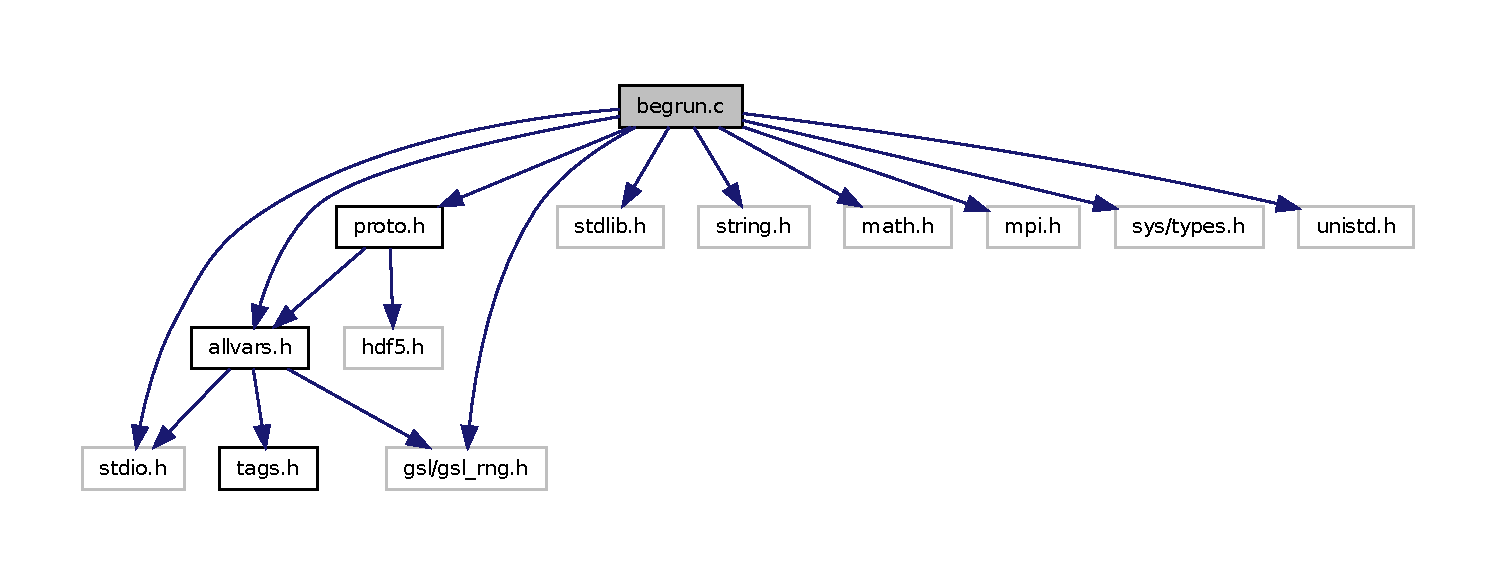
\includegraphics[width=400pt]{begrun_8c__incl}
\end{center}
\end{figure}
\subsection*{Defines}
\begin{DoxyCompactItemize}
\item 
\#define \hyperlink{begrun_8c_a8747af38b86aa2bbcda2f1b1aa0888c2}{DOUBLE}~1
\item 
\#define \hyperlink{begrun_8c_a0f4d394a3ab4e09bff60f714c66dc5ee}{STRING}~2
\item 
\#define \hyperlink{begrun_8c_afeeffe52c8fd59db7c61cf8b02042dbf}{INT}~3
\item 
\#define \hyperlink{begrun_8c_a80a3e5dc9fa74f5cba16d39307f148e0}{MAXTAGS}~300
\end{DoxyCompactItemize}
\subsection*{Functions}
\begin{DoxyCompactItemize}
\item 
void \hyperlink{begrun_8c_aceeb5c8909331b90ea8345e0fc853f82}{begrun} (void)
\item 
void \hyperlink{begrun_8c_aba986f6be1d66945199c7ea43e5c9610}{set\_\-units} (void)
\item 
void \hyperlink{begrun_8c_a6f629274f7b036874c743fb81d58ce68}{open\_\-outputfiles} (void)
\item 
void \hyperlink{begrun_8c_aa1abb9ee0e0a43ec19cdaa55c8ecd43c}{close\_\-outputfiles} (void)
\item 
void \hyperlink{begrun_8c_a952eae1977b498c4fdfabed1742a3ba2}{read\_\-parameter\_\-file} (char $\ast$fname)
\item 
int \hyperlink{begrun_8c_a849a294ac908c933ffb82dc4319af513}{read\_\-outputlist} (char $\ast$fname)
\item 
void \hyperlink{begrun_8c_acc4d1f5e4e51140090a7ce25ea263b98}{readjust\_\-timebase} (double TimeMax\_\-old, double TimeMax\_\-new)
\end{DoxyCompactItemize}


\subsection{Detailed Description}
initial set-\/up of a simulation run This file contains various functions to initialize a simulation run. In particular, the parameterfile is read in and parsed, the initial conditions or restart files are read, and global variables are initialized to their proper values. 

Definition in file \hyperlink{begrun_8c_source}{begrun.c}.



\subsection{Define Documentation}
\hypertarget{begrun_8c_a8747af38b86aa2bbcda2f1b1aa0888c2}{
\index{begrun.c@{begrun.c}!DOUBLE@{DOUBLE}}
\index{DOUBLE@{DOUBLE}!begrun.c@{begrun.c}}
\subsubsection[{DOUBLE}]{\setlength{\rightskip}{0pt plus 5cm}\#define DOUBLE~1}}
\label{begrun_8c_a8747af38b86aa2bbcda2f1b1aa0888c2}


Referenced by read\_\-parameter\_\-file().

\hypertarget{begrun_8c_afeeffe52c8fd59db7c61cf8b02042dbf}{
\index{begrun.c@{begrun.c}!INT@{INT}}
\index{INT@{INT}!begrun.c@{begrun.c}}
\subsubsection[{INT}]{\setlength{\rightskip}{0pt plus 5cm}\#define INT~3}}
\label{begrun_8c_afeeffe52c8fd59db7c61cf8b02042dbf}


Referenced by read\_\-parameter\_\-file().

\hypertarget{begrun_8c_a80a3e5dc9fa74f5cba16d39307f148e0}{
\index{begrun.c@{begrun.c}!MAXTAGS@{MAXTAGS}}
\index{MAXTAGS@{MAXTAGS}!begrun.c@{begrun.c}}
\subsubsection[{MAXTAGS}]{\setlength{\rightskip}{0pt plus 5cm}\#define MAXTAGS~300}}
\label{begrun_8c_a80a3e5dc9fa74f5cba16d39307f148e0}
\hypertarget{begrun_8c_a0f4d394a3ab4e09bff60f714c66dc5ee}{
\index{begrun.c@{begrun.c}!STRING@{STRING}}
\index{STRING@{STRING}!begrun.c@{begrun.c}}
\subsubsection[{STRING}]{\setlength{\rightskip}{0pt plus 5cm}\#define STRING~2}}
\label{begrun_8c_a0f4d394a3ab4e09bff60f714c66dc5ee}


Referenced by read\_\-parameter\_\-file().



\subsection{Function Documentation}
\hypertarget{begrun_8c_aceeb5c8909331b90ea8345e0fc853f82}{
\index{begrun.c@{begrun.c}!begrun@{begrun}}
\index{begrun@{begrun}!begrun.c@{begrun.c}}
\subsubsection[{begrun}]{\setlength{\rightskip}{0pt plus 5cm}void begrun (
\begin{DoxyParamCaption}
\item[{void}]{}
\end{DoxyParamCaption}
)}}
\label{begrun_8c_aceeb5c8909331b90ea8345e0fc853f82}
This function performs the initial set-\/up of the simulation. First, the parameterfile is set, then routines for setting units, reading ICs/restart-\/files are called, auxialiary memory is allocated, etc. 

$<$ code version string 



Definition at line 28 of file begrun.c.



References All, allocate\_\-commbuffers(), AllocateInteractionTable(), global\_\-data\_\-all\_\-processes::ArtBulkViscConst, global\_\-data\_\-all\_\-processes::BufferSize, global\_\-data\_\-all\_\-processes::BunchSizeDensity, global\_\-data\_\-all\_\-processes::BunchSizeDomain, global\_\-data\_\-all\_\-processes::BunchSizeForce, global\_\-data\_\-all\_\-processes::BunchSizeHydro, global\_\-data\_\-all\_\-processes::ComovingIntegrationOn, global\_\-data\_\-all\_\-processes::CourantFac, global\_\-data\_\-all\_\-processes::CpuFile, CPUThisRun, global\_\-data\_\-all\_\-processes::CpuTimeBetRestartFile, global\_\-data\_\-all\_\-processes::EnergyFile, global\_\-data\_\-all\_\-processes::ErrTolForceAcc, global\_\-data\_\-all\_\-processes::ErrTolIntAccuracy, ewald\_\-init(), find\_\-next\_\-outputtime(), GADGETVERSION, global\_\-data\_\-all\_\-processes::InfoFile, init(), init\_\-drift\_\-table(), init\_\-geofactor\_\-table(), long\_\-range\_\-init(), long\_\-range\_\-init\_\-regionsize(), global\_\-data\_\-all\_\-processes::MaxNumNgbDeviation, global\_\-data\_\-all\_\-processes::MaxRMSDisplacementFac, global\_\-data\_\-all\_\-processes::MaxSizeTimestep, global\_\-data\_\-all\_\-processes::MinSizeTimestep, NTask, global\_\-data\_\-all\_\-processes::NumFilesPerSnapshot, global\_\-data\_\-all\_\-processes::NumFilesWrittenInParallel, open\_\-outputfiles(), global\_\-data\_\-all\_\-processes::OutputDir, global\_\-data\_\-all\_\-processes::OutputListFilename, global\_\-data\_\-all\_\-processes::OutputListLength, global\_\-data\_\-all\_\-processes::OutputListOn, global\_\-data\_\-all\_\-processes::OutputListTimes, ParameterFile, random\_\-generator, read\_\-parameter\_\-file(), readjust\_\-timebase(), restart(), global\_\-data\_\-all\_\-processes::RestartFile, RestartFlag, global\_\-data\_\-all\_\-processes::ResubmitCommand, global\_\-data\_\-all\_\-processes::ResubmitOn, set\_\-random\_\-numbers(), set\_\-units(), global\_\-data\_\-all\_\-processes::SnapFormat, global\_\-data\_\-all\_\-processes::SnapshotFileBase, ThisTask, global\_\-data\_\-all\_\-processes::Ti\_\-Current, global\_\-data\_\-all\_\-processes::Ti\_\-nextoutput, global\_\-data\_\-all\_\-processes::TimeBetSnapshot, global\_\-data\_\-all\_\-processes::TimeBetStatistics, global\_\-data\_\-all\_\-processes::TimeLastRestartFile, global\_\-data\_\-all\_\-processes::TimeLimitCPU, global\_\-data\_\-all\_\-processes::TimeMax, global\_\-data\_\-all\_\-processes::TimingsFile, global\_\-data\_\-all\_\-processes::TreeDomainUpdateFrequency, global\_\-data\_\-all\_\-processes::TypeOfOpeningCriterion, and global\_\-data\_\-all\_\-processes::TypeOfTimestepCriterion.



Referenced by main().




\begin{DoxyCode}
{
  struct global_data_all_processes all;

  if(ThisTask == 0)
    {
      printf("\nThis is Gadget, version `%s'.\n", GADGETVERSION);
      printf("\nRunning on %d processors.\n", NTask);
    }

  read_parameter_file(ParameterFile);   /* ... read in parameters for this run */
      

  allocate_commbuffers();       /* ... allocate buffer-memory for particle 
                                   exchange during force computation */
  set_units();

#if defined(PERIODIC) && (!defined(PMGRID) || defined(FORCETEST))
  ewald_init();
#endif

  open_outputfiles();

  random_generator = gsl_rng_alloc(gsl_rng_ranlxd1);
  gsl_rng_set(random_generator, 42);    /* start-up seed */

#ifdef PMGRID
  long_range_init();
#endif

  All.TimeLastRestartFile = CPUThisRun;

#ifdef COMPUTE_SELFINTERACTION_FORDARK
  AllocateInteractionTable(INTERACTION_TABLE_LENGTH, PARTICLE_MAX_INTERACTIONS + 
      1);
  init_geofactor_table();
#endif

  if(RestartFlag == 0 || RestartFlag == 2)
    {
      set_random_numbers();

      init();                   /* ... read in initial model */
    }
  else
    {
      all = All;                /* save global variables. (will be read from rest
      art file) */

      restart(RestartFlag);     /* ... read restart file. Note: This also resets 
      
                                   all variables in the struct `All'. 
                                   However, during the run, some variables in the
       parameter
                                   file are allowed to be changed, if desired. Th
      ese need to 
                                   copied in the way below.
                                   Note:  All.PartAllocFactor is treated in resta
      rt() separately.  
                                 */

      All.MinSizeTimestep = all.MinSizeTimestep;
      All.MaxSizeTimestep = all.MaxSizeTimestep;
      All.BufferSize = all.BufferSize;
      All.BunchSizeForce = all.BunchSizeForce;
      All.BunchSizeDensity = all.BunchSizeDensity;
      All.BunchSizeHydro = all.BunchSizeHydro;
      All.BunchSizeDomain = all.BunchSizeDomain;

      All.TimeLimitCPU = all.TimeLimitCPU;
      All.ResubmitOn = all.ResubmitOn;
      All.TimeBetSnapshot = all.TimeBetSnapshot;
      All.TimeBetStatistics = all.TimeBetStatistics;
      All.CpuTimeBetRestartFile = all.CpuTimeBetRestartFile;
      All.ErrTolIntAccuracy = all.ErrTolIntAccuracy;
      All.MaxRMSDisplacementFac = all.MaxRMSDisplacementFac;

      All.ErrTolForceAcc = all.ErrTolForceAcc;

      All.TypeOfTimestepCriterion = all.TypeOfTimestepCriterion;
      All.TypeOfOpeningCriterion = all.TypeOfOpeningCriterion;
      All.NumFilesWrittenInParallel = all.NumFilesWrittenInParallel;
      All.TreeDomainUpdateFrequency = all.TreeDomainUpdateFrequency;

      All.SnapFormat = all.SnapFormat;
      All.NumFilesPerSnapshot = all.NumFilesPerSnapshot;
      All.MaxNumNgbDeviation = all.MaxNumNgbDeviation;
      All.ArtBulkViscConst = all.ArtBulkViscConst;


      All.OutputListOn = all.OutputListOn;
      All.CourantFac = all.CourantFac;

      All.OutputListLength = all.OutputListLength;
      memcpy(All.OutputListTimes, all.OutputListTimes, sizeof(double) * All.
      OutputListLength);


      strcpy(All.ResubmitCommand, all.ResubmitCommand);
      strcpy(All.OutputListFilename, all.OutputListFilename);
      strcpy(All.OutputDir, all.OutputDir);
      strcpy(All.RestartFile, all.RestartFile);
      strcpy(All.EnergyFile, all.EnergyFile);
      strcpy(All.InfoFile, all.InfoFile);
      strcpy(All.CpuFile, all.CpuFile);
      strcpy(All.TimingsFile, all.TimingsFile);
      strcpy(All.SnapshotFileBase, all.SnapshotFileBase);

      if(All.TimeMax != all.TimeMax)
        readjust_timebase(All.TimeMax, all.TimeMax);
    }

#ifdef PMGRID
  long_range_init_regionsize();
#endif
 
  if(All.ComovingIntegrationOn)
    init_drift_table();

  if(RestartFlag == 2)
    All.Ti_nextoutput = find_next_outputtime(All.Ti_Current + 1);
  else
    All.Ti_nextoutput = find_next_outputtime(All.Ti_Current);


  All.TimeLastRestartFile = CPUThisRun;
}
\end{DoxyCode}




Here is the call graph for this function:
\nopagebreak
\begin{figure}[H]
\begin{center}
\leavevmode
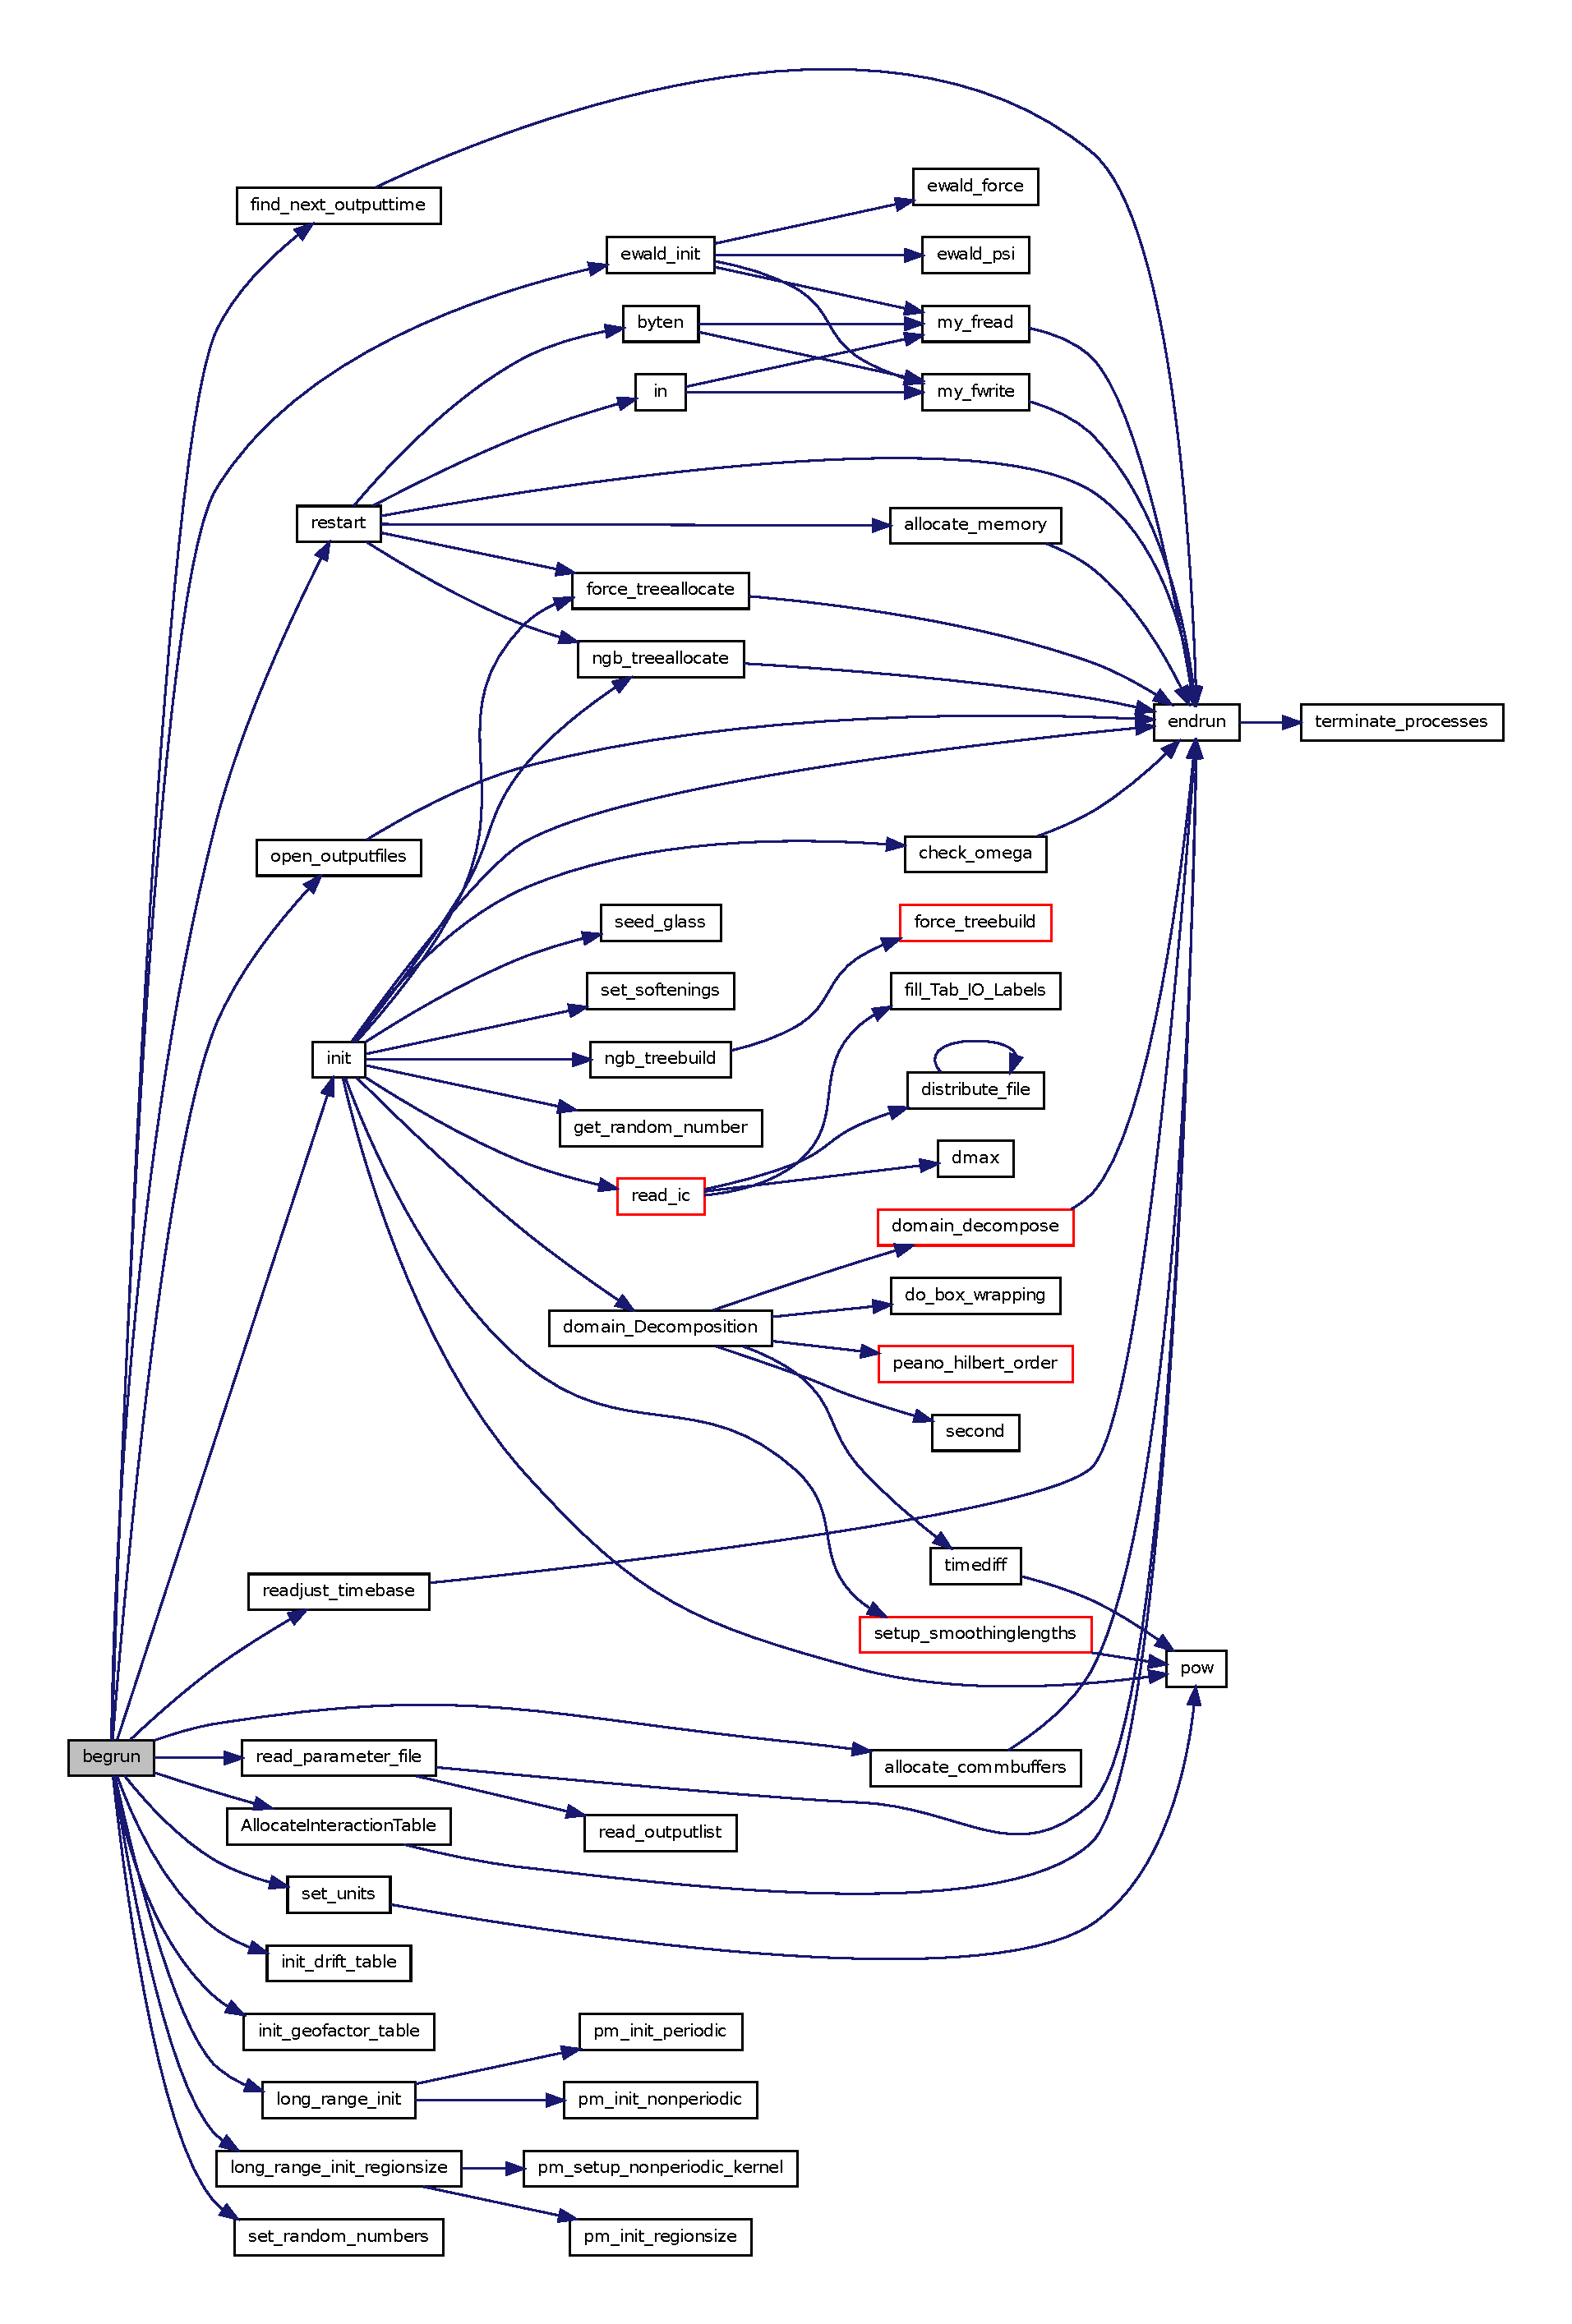
\includegraphics[width=400pt]{begrun_8c_aceeb5c8909331b90ea8345e0fc853f82_cgraph}
\end{center}
\end{figure}




Here is the caller graph for this function:
\nopagebreak
\begin{figure}[H]
\begin{center}
\leavevmode
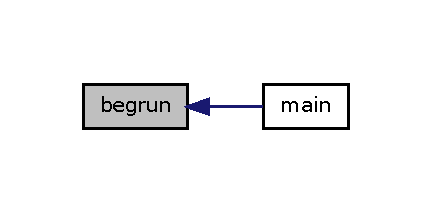
\includegraphics[width=208pt]{begrun_8c_aceeb5c8909331b90ea8345e0fc853f82_icgraph}
\end{center}
\end{figure}


\hypertarget{begrun_8c_aa1abb9ee0e0a43ec19cdaa55c8ecd43c}{
\index{begrun.c@{begrun.c}!close\_\-outputfiles@{close\_\-outputfiles}}
\index{close\_\-outputfiles@{close\_\-outputfiles}!begrun.c@{begrun.c}}
\subsubsection[{close\_\-outputfiles}]{\setlength{\rightskip}{0pt plus 5cm}void close\_\-outputfiles (
\begin{DoxyParamCaption}
\item[{void}]{}
\end{DoxyParamCaption}
)}}
\label{begrun_8c_aa1abb9ee0e0a43ec19cdaa55c8ecd43c}
This function closes the global log-\/files. 

Definition at line 262 of file begrun.c.



References FdCPU, FdEnergy, FdForceTest, FdInfo, FdTimings, and ThisTask.



Referenced by run().




\begin{DoxyCode}
{
  if(ThisTask != 0)             /* only the root processor writes to the log file
      s */
    return;

  fclose(FdCPU);
  fclose(FdInfo);
  fclose(FdEnergy);
  fclose(FdTimings);
#ifdef FORCETEST
  fclose(FdForceTest);
#endif
}
\end{DoxyCode}




Here is the caller graph for this function:
\nopagebreak
\begin{figure}[H]
\begin{center}
\leavevmode
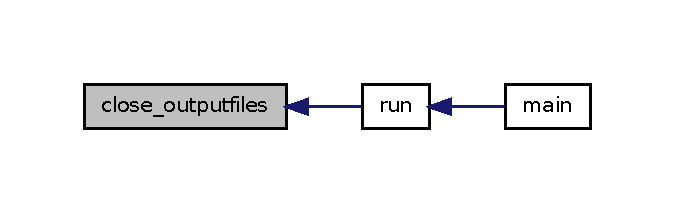
\includegraphics[width=324pt]{begrun_8c_aa1abb9ee0e0a43ec19cdaa55c8ecd43c_icgraph}
\end{center}
\end{figure}


\hypertarget{begrun_8c_a6f629274f7b036874c743fb81d58ce68}{
\index{begrun.c@{begrun.c}!open\_\-outputfiles@{open\_\-outputfiles}}
\index{open\_\-outputfiles@{open\_\-outputfiles}!begrun.c@{begrun.c}}
\subsubsection[{open\_\-outputfiles}]{\setlength{\rightskip}{0pt plus 5cm}void open\_\-outputfiles (
\begin{DoxyParamCaption}
\item[{void}]{}
\end{DoxyParamCaption}
)}}
\label{begrun_8c_a6f629274f7b036874c743fb81d58ce68}
This function opens various log-\/files that report on the status and performance of the simulstion. On restart from restart-\/files (start-\/option 1), the code will append to these files. 

Definition at line 204 of file begrun.c.



References All, global\_\-data\_\-all\_\-processes::CpuFile, endrun(), global\_\-data\_\-all\_\-processes::EnergyFile, FdCPU, FdEnergy, FdForceTest, FdInfo, FdTimings, global\_\-data\_\-all\_\-processes::InfoFile, global\_\-data\_\-all\_\-processes::OutputDir, RestartFlag, ThisTask, and global\_\-data\_\-all\_\-processes::TimingsFile.



Referenced by begrun().




\begin{DoxyCode}
{
  char mode[2], buf[200];

  if(ThisTask != 0)             /* only the root processor writes to the log file
      s */
    return;

  if(RestartFlag == 0)
    strcpy(mode, "w");
  else
    strcpy(mode, "a");


  sprintf(buf, "%s%s", All.OutputDir, All.CpuFile);
  if(!(FdCPU = fopen(buf, mode)))
    {
      printf("error in opening file '%s'\n", buf);
      endrun(1);
    }

  sprintf(buf, "%s%s", All.OutputDir, All.InfoFile);
  if(!(FdInfo = fopen(buf, mode)))
    {
      printf("error in opening file '%s'\n", buf);
      endrun(1);
    }

  sprintf(buf, "%s%s", All.OutputDir, All.EnergyFile);
  if(!(FdEnergy = fopen(buf, mode)))
    {
      printf("error in opening file '%s'\n", buf);
      endrun(1);
    }

  sprintf(buf, "%s%s", All.OutputDir, All.TimingsFile);
  if(!(FdTimings = fopen(buf, mode)))
    {
      printf("error in opening file '%s'\n", buf);
      endrun(1);
    }

#ifdef FORCETEST
  if(RestartFlag == 0)
    {
      sprintf(buf, "%s%s", All.OutputDir, "forcetest.txt");
      if(!(FdForceTest = fopen(buf, "w")))
        {
          printf("error in opening file '%s'\n", buf);
          endrun(1);
        }
      fclose(FdForceTest);
    }
#endif
}
\end{DoxyCode}




Here is the call graph for this function:
\nopagebreak
\begin{figure}[H]
\begin{center}
\leavevmode
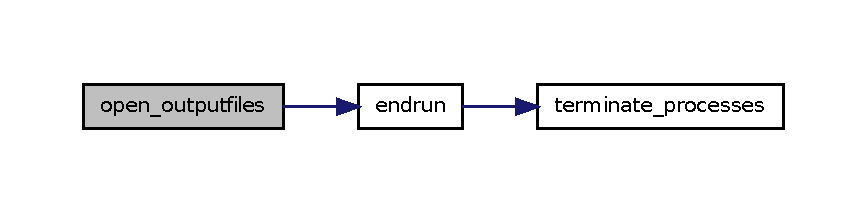
\includegraphics[width=400pt]{begrun_8c_a6f629274f7b036874c743fb81d58ce68_cgraph}
\end{center}
\end{figure}




Here is the caller graph for this function:
\nopagebreak
\begin{figure}[H]
\begin{center}
\leavevmode
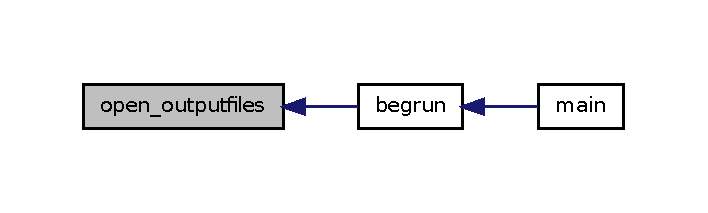
\includegraphics[width=340pt]{begrun_8c_a6f629274f7b036874c743fb81d58ce68_icgraph}
\end{center}
\end{figure}


\hypertarget{begrun_8c_a849a294ac908c933ffb82dc4319af513}{
\index{begrun.c@{begrun.c}!read\_\-outputlist@{read\_\-outputlist}}
\index{read\_\-outputlist@{read\_\-outputlist}!begrun.c@{begrun.c}}
\subsubsection[{read\_\-outputlist}]{\setlength{\rightskip}{0pt plus 5cm}int read\_\-outputlist (
\begin{DoxyParamCaption}
\item[{char $\ast$}]{ fname}
\end{DoxyParamCaption}
)}}
\label{begrun_8c_a849a294ac908c933ffb82dc4319af513}
this function reads a table with a list of desired output times. The table does not have to be ordered in any way, but may not contain more than MAXLEN\_\-OUTPUTLIST entries. 

$<$ maxmimum number of entries in list of snapshot output times 



Definition at line 770 of file begrun.c.



References All, fd, MAXLEN\_\-OUTPUTLIST, global\_\-data\_\-all\_\-processes::OutputListLength, and global\_\-data\_\-all\_\-processes::OutputListTimes.



Referenced by read\_\-parameter\_\-file().




\begin{DoxyCode}
{
  FILE *fd;

  if(!(fd = fopen(fname, "r")))
    {
      printf("can't read output list in file '%s'\n", fname);
      return 1;
    }

  All.OutputListLength = 0;
  do
    {
      if(fscanf(fd, " %lg ", &All.OutputListTimes[All.OutputListLength]) == 1)
        All.OutputListLength++;
      else
        break;
    }
  while(All.OutputListLength < MAXLEN_OUTPUTLIST);

  fclose(fd);

  printf("\nfound %d times in output-list.\n", All.OutputListLength);

  return 0;
}
\end{DoxyCode}




Here is the caller graph for this function:
\nopagebreak
\begin{figure}[H]
\begin{center}
\leavevmode
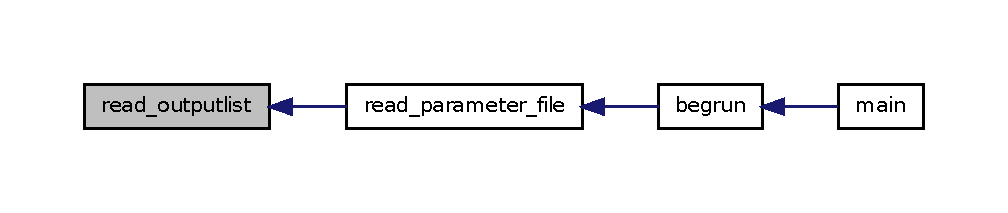
\includegraphics[width=400pt]{begrun_8c_a849a294ac908c933ffb82dc4319af513_icgraph}
\end{center}
\end{figure}


\hypertarget{begrun_8c_a952eae1977b498c4fdfabed1742a3ba2}{
\index{begrun.c@{begrun.c}!read\_\-parameter\_\-file@{read\_\-parameter\_\-file}}
\index{read\_\-parameter\_\-file@{read\_\-parameter\_\-file}!begrun.c@{begrun.c}}
\subsubsection[{read\_\-parameter\_\-file}]{\setlength{\rightskip}{0pt plus 5cm}void read\_\-parameter\_\-file (
\begin{DoxyParamCaption}
\item[{char $\ast$}]{ fname}
\end{DoxyParamCaption}
)}}
\label{begrun_8c_a952eae1977b498c4fdfabed1742a3ba2}
This function parses the parameterfile in a simple way. Each paramater is defined by a keyword (`tag'), and can be either of type double, int, or character string. The routine makes sure that each parameter appears exactly once in the parameterfile, otherwise error messages are produced that complain about the missing parameters. 

Definition at line 285 of file begrun.c.



References All, global\_\-data\_\-all\_\-processes::ArtBulkViscConst, global\_\-data\_\-all\_\-processes::BoxSize, global\_\-data\_\-all\_\-processes::BufferSize, global\_\-data\_\-all\_\-processes::ComovingIntegrationOn, global\_\-data\_\-all\_\-processes::CourantFac, global\_\-data\_\-all\_\-processes::CpuFile, global\_\-data\_\-all\_\-processes::CpuTimeBetRestartFile, global\_\-data\_\-all\_\-processes::DesNumNgb, DOUBLE, endrun(), global\_\-data\_\-all\_\-processes::EnergyFile, global\_\-data\_\-all\_\-processes::ErrTolForceAcc, global\_\-data\_\-all\_\-processes::ErrTolIntAccuracy, global\_\-data\_\-all\_\-processes::ErrTolTheta, fd, global\_\-data\_\-all\_\-processes::GravityConstantInternal, global\_\-data\_\-all\_\-processes::HubbleParam, global\_\-data\_\-all\_\-processes::ICFormat, global\_\-data\_\-all\_\-processes::InfoFile, global\_\-data\_\-all\_\-processes::InitCondFile, global\_\-data\_\-all\_\-processes::InitGasTemp, INT, global\_\-data\_\-all\_\-processes::MaxNumNgbDeviation, global\_\-data\_\-all\_\-processes::MaxRMSDisplacementFac, global\_\-data\_\-all\_\-processes::MaxSizeTimestep, global\_\-data\_\-all\_\-processes::MinGasHsmlFractional, global\_\-data\_\-all\_\-processes::MinGasTemp, global\_\-data\_\-all\_\-processes::MinSizeTimestep, NTask, global\_\-data\_\-all\_\-processes::NumFilesPerSnapshot, global\_\-data\_\-all\_\-processes::NumFilesWrittenInParallel, global\_\-data\_\-all\_\-processes::Omega0, global\_\-data\_\-all\_\-processes::OmegaBaryon, global\_\-data\_\-all\_\-processes::OmegaLambda, global\_\-data\_\-all\_\-processes::OutputDir, global\_\-data\_\-all\_\-processes::OutputListFilename, global\_\-data\_\-all\_\-processes::OutputListLength, global\_\-data\_\-all\_\-processes::OutputListOn, global\_\-data\_\-all\_\-processes::PartAllocFactor, global\_\-data\_\-all\_\-processes::PeriodicBoundariesOn, read\_\-outputlist(), global\_\-data\_\-all\_\-processes::RestartFile, global\_\-data\_\-all\_\-processes::ResubmitCommand, global\_\-data\_\-all\_\-processes::ResubmitOn, global\_\-data\_\-all\_\-processes::SnapFormat, global\_\-data\_\-all\_\-processes::SnapshotFileBase, global\_\-data\_\-all\_\-processes::SofteningBndry, global\_\-data\_\-all\_\-processes::SofteningBndryMaxPhys, global\_\-data\_\-all\_\-processes::SofteningBulge, global\_\-data\_\-all\_\-processes::SofteningBulgeMaxPhys, global\_\-data\_\-all\_\-processes::SofteningDisk, global\_\-data\_\-all\_\-processes::SofteningDiskMaxPhys, global\_\-data\_\-all\_\-processes::SofteningGas, global\_\-data\_\-all\_\-processes::SofteningGasMaxPhys, global\_\-data\_\-all\_\-processes::SofteningHalo, global\_\-data\_\-all\_\-processes::SofteningHaloMaxPhys, global\_\-data\_\-all\_\-processes::SofteningStars, global\_\-data\_\-all\_\-processes::SofteningStarsMaxPhys, STRING, ThisTask, global\_\-data\_\-all\_\-processes::TimeBegin, global\_\-data\_\-all\_\-processes::TimeBetSnapshot, global\_\-data\_\-all\_\-processes::TimeBetStatistics, global\_\-data\_\-all\_\-processes::TimeLimitCPU, global\_\-data\_\-all\_\-processes::TimeMax, global\_\-data\_\-all\_\-processes::TimeOfFirstSnapshot, global\_\-data\_\-all\_\-processes::TimingsFile, global\_\-data\_\-all\_\-processes::TreeAllocFactor, global\_\-data\_\-all\_\-processes::TreeDomainUpdateFrequency, global\_\-data\_\-all\_\-processes::TypeOfOpeningCriterion, global\_\-data\_\-all\_\-processes::TypeOfTimestepCriterion, global\_\-data\_\-all\_\-processes::UnitLength\_\-in\_\-cm, global\_\-data\_\-all\_\-processes::UnitMass\_\-in\_\-g, and global\_\-data\_\-all\_\-processes::UnitVelocity\_\-in\_\-cm\_\-per\_\-s.



Referenced by begrun().




\begin{DoxyCode}
{
#define DOUBLE 1
#define STRING 2
#define INT 3
#define MAXTAGS 300

  FILE *fd, *fdout;
  char buf[200], buf1[200], buf2[200], buf3[400];
  int i, j, nt;
  int id[MAXTAGS];
  void *addr[MAXTAGS];
  char tag[MAXTAGS][50];
  int  errorFlag = 0;


  if(sizeof(long long) != 8)
    {
      if(ThisTask == 0)
        printf("\nType `long long' is not 64 bit on this platform. Stopping.\n\n"
      );
      endrun(0);
    }

  if(sizeof(int) != 4)
    {
      if(ThisTask == 0)
        printf("\nType `int' is not 32 bit on this platform. Stopping.\n\n");
      endrun(0);
    }

  if(sizeof(float) != 4)
    {
      if(ThisTask == 0)
        printf("\nType `float' is not 32 bit on this platform. Stopping.\n\n");
      endrun(0);
    }

  if(sizeof(double) != 8)
    {
      if(ThisTask == 0)
        printf("\nType `double' is not 64 bit on this platform. Stopping.\n\n");
      endrun(0);
    }


  if(ThisTask == 0)             /* read parameter file on process 0 */
    {
      nt = 0;

      strcpy(tag[nt], "InitCondFile");
      addr[nt] = All.InitCondFile;
      id[nt++] = STRING;

      strcpy(tag[nt], "OutputDir");
      addr[nt] = All.OutputDir;
      id[nt++] = STRING;

      strcpy(tag[nt], "SnapshotFileBase");
      addr[nt] = All.SnapshotFileBase;
      id[nt++] = STRING;

      strcpy(tag[nt], "EnergyFile");
      addr[nt] = All.EnergyFile;
      id[nt++] = STRING;

      strcpy(tag[nt], "CpuFile");
      addr[nt] = All.CpuFile;
      id[nt++] = STRING;

      strcpy(tag[nt], "InfoFile");
      addr[nt] = All.InfoFile;
      id[nt++] = STRING;

      strcpy(tag[nt], "TimingsFile");
      addr[nt] = All.TimingsFile;
      id[nt++] = STRING;

      strcpy(tag[nt], "RestartFile");
      addr[nt] = All.RestartFile;
      id[nt++] = STRING;

      strcpy(tag[nt], "ResubmitCommand");
      addr[nt] = All.ResubmitCommand;
      id[nt++] = STRING;

      strcpy(tag[nt], "OutputListFilename");
      addr[nt] = All.OutputListFilename;
      id[nt++] = STRING;

      strcpy(tag[nt], "OutputListOn");
      addr[nt] = &All.OutputListOn;
      id[nt++] = INT;

      strcpy(tag[nt], "Omega0");
      addr[nt] = &All.Omega0;
      id[nt++] = DOUBLE;

      strcpy(tag[nt], "OmegaBaryon");
      addr[nt] = &All.OmegaBaryon;
      id[nt++] = DOUBLE;

      strcpy(tag[nt], "OmegaLambda");
      addr[nt] = &All.OmegaLambda;
      id[nt++] = DOUBLE;

      strcpy(tag[nt], "HubbleParam");
      addr[nt] = &All.HubbleParam;
      id[nt++] = DOUBLE;

      strcpy(tag[nt], "BoxSize");
      addr[nt] = &All.BoxSize;
      id[nt++] = DOUBLE;

      strcpy(tag[nt], "PeriodicBoundariesOn");
      addr[nt] = &All.PeriodicBoundariesOn;
      id[nt++] = INT;

      strcpy(tag[nt], "TimeOfFirstSnapshot");
      addr[nt] = &All.TimeOfFirstSnapshot;
      id[nt++] = DOUBLE;

      strcpy(tag[nt], "CpuTimeBetRestartFile");
      addr[nt] = &All.CpuTimeBetRestartFile;
      id[nt++] = DOUBLE;

      strcpy(tag[nt], "TimeBetStatistics");
      addr[nt] = &All.TimeBetStatistics;
      id[nt++] = DOUBLE;

      strcpy(tag[nt], "TimeBegin");
      addr[nt] = &All.TimeBegin;
      id[nt++] = DOUBLE;

      strcpy(tag[nt], "TimeMax");
      addr[nt] = &All.TimeMax;
      id[nt++] = DOUBLE;

      strcpy(tag[nt], "TimeBetSnapshot");
      addr[nt] = &All.TimeBetSnapshot;
      id[nt++] = DOUBLE;

      strcpy(tag[nt], "UnitVelocity_in_cm_per_s");
      addr[nt] = &All.UnitVelocity_in_cm_per_s;
      id[nt++] = DOUBLE;

      strcpy(tag[nt], "UnitLength_in_cm");
      addr[nt] = &All.UnitLength_in_cm;
      id[nt++] = DOUBLE;

      strcpy(tag[nt], "UnitMass_in_g");
      addr[nt] = &All.UnitMass_in_g;
      id[nt++] = DOUBLE;

      strcpy(tag[nt], "TreeDomainUpdateFrequency");
      addr[nt] = &All.TreeDomainUpdateFrequency;
      id[nt++] = DOUBLE;

      strcpy(tag[nt], "ErrTolIntAccuracy");
      addr[nt] = &All.ErrTolIntAccuracy;
      id[nt++] = DOUBLE;

      strcpy(tag[nt], "ErrTolTheta");
      addr[nt] = &All.ErrTolTheta;
      id[nt++] = DOUBLE;

      strcpy(tag[nt], "ErrTolForceAcc");
      addr[nt] = &All.ErrTolForceAcc;
      id[nt++] = DOUBLE;

      strcpy(tag[nt], "MinGasHsmlFractional");
      addr[nt] = &All.MinGasHsmlFractional;
      id[nt++] = DOUBLE;

      strcpy(tag[nt], "MaxSizeTimestep");
      addr[nt] = &All.MaxSizeTimestep;
      id[nt++] = DOUBLE;

      strcpy(tag[nt], "MinSizeTimestep");
      addr[nt] = &All.MinSizeTimestep;
      id[nt++] = DOUBLE;

      strcpy(tag[nt], "MaxRMSDisplacementFac");
      addr[nt] = &All.MaxRMSDisplacementFac;
      id[nt++] = DOUBLE;

      strcpy(tag[nt], "ArtBulkViscConst");
      addr[nt] = &All.ArtBulkViscConst;
      id[nt++] = DOUBLE;

      strcpy(tag[nt], "CourantFac");
      addr[nt] = &All.CourantFac;
      id[nt++] = DOUBLE;

      strcpy(tag[nt], "DesNumNgb");
      addr[nt] = &All.DesNumNgb;
      id[nt++] = DOUBLE;

      strcpy(tag[nt], "MaxNumNgbDeviation");
      addr[nt] = &All.MaxNumNgbDeviation;
      id[nt++] = DOUBLE;

      strcpy(tag[nt], "ComovingIntegrationOn");
      addr[nt] = &All.ComovingIntegrationOn;
      id[nt++] = INT;

      strcpy(tag[nt], "ICFormat");
      addr[nt] = &All.ICFormat;
      id[nt++] = INT;

      strcpy(tag[nt], "SnapFormat");
      addr[nt] = &All.SnapFormat;
      id[nt++] = INT;

      strcpy(tag[nt], "NumFilesPerSnapshot");
      addr[nt] = &All.NumFilesPerSnapshot;
      id[nt++] = INT;

      strcpy(tag[nt], "NumFilesWrittenInParallel");
      addr[nt] = &All.NumFilesWrittenInParallel;
      id[nt++] = INT;

      strcpy(tag[nt], "ResubmitOn");
      addr[nt] = &All.ResubmitOn;
      id[nt++] = INT;

      strcpy(tag[nt], "TypeOfTimestepCriterion");
      addr[nt] = &All.TypeOfTimestepCriterion;
      id[nt++] = INT;

      strcpy(tag[nt], "TypeOfOpeningCriterion");
      addr[nt] = &All.TypeOfOpeningCriterion;
      id[nt++] = INT;

      strcpy(tag[nt], "TimeLimitCPU");
      addr[nt] = &All.TimeLimitCPU;
      id[nt++] = DOUBLE;

      strcpy(tag[nt], "SofteningHalo");
      addr[nt] = &All.SofteningHalo;
      id[nt++] = DOUBLE;

      strcpy(tag[nt], "SofteningDisk");
      addr[nt] = &All.SofteningDisk;
      id[nt++] = DOUBLE;

      strcpy(tag[nt], "SofteningBulge");
      addr[nt] = &All.SofteningBulge;
      id[nt++] = DOUBLE;

      strcpy(tag[nt], "SofteningGas");
      addr[nt] = &All.SofteningGas;
      id[nt++] = DOUBLE;

      strcpy(tag[nt], "SofteningStars");
      addr[nt] = &All.SofteningStars;
      id[nt++] = DOUBLE;

      strcpy(tag[nt], "SofteningBndry");
      addr[nt] = &All.SofteningBndry;
      id[nt++] = DOUBLE;

      strcpy(tag[nt], "SofteningHaloMaxPhys");
      addr[nt] = &All.SofteningHaloMaxPhys;
      id[nt++] = DOUBLE;

      strcpy(tag[nt], "SofteningDiskMaxPhys");
      addr[nt] = &All.SofteningDiskMaxPhys;
      id[nt++] = DOUBLE;

      strcpy(tag[nt], "SofteningBulgeMaxPhys");
      addr[nt] = &All.SofteningBulgeMaxPhys;
      id[nt++] = DOUBLE;

      strcpy(tag[nt], "SofteningGasMaxPhys");
      addr[nt] = &All.SofteningGasMaxPhys;
      id[nt++] = DOUBLE;

      strcpy(tag[nt], "SofteningStarsMaxPhys");
      addr[nt] = &All.SofteningStarsMaxPhys;
      id[nt++] = DOUBLE;

      strcpy(tag[nt], "SofteningBndryMaxPhys");
      addr[nt] = &All.SofteningBndryMaxPhys;
      id[nt++] = DOUBLE;

      strcpy(tag[nt], "BufferSize");
      addr[nt] = &All.BufferSize;
      id[nt++] = INT;

      strcpy(tag[nt], "PartAllocFactor");
      addr[nt] = &All.PartAllocFactor;
      id[nt++] = DOUBLE;

      strcpy(tag[nt], "TreeAllocFactor");
      addr[nt] = &All.TreeAllocFactor;
      id[nt++] = DOUBLE;

      strcpy(tag[nt], "GravityConstantInternal");
      addr[nt] = &All.GravityConstantInternal;
      id[nt++] = DOUBLE;

      strcpy(tag[nt], "InitGasTemp");
      addr[nt] = &All.InitGasTemp;
      id[nt++] = DOUBLE;

      strcpy(tag[nt], "MinGasTemp");
      addr[nt] = &All.MinGasTemp;
      id[nt++] = DOUBLE;

#ifdef COMPUTE_SELFINTERACTION_FORDARK 
      strcpy(tag[nt], "InteractionCrossSection");
      addr[nt] = &All.InteractionCrossSection;
      id[nt++] = DOUBLE;
#endif

      if((fd = fopen(fname, "r")))
        {
          sprintf(buf, "%s%s", fname, "-usedvalues");
          if(!(fdout = fopen(buf, "w")))
            {
              printf("error opening file '%s' \n", buf);
              errorFlag = 1;
            }
          else
            {
              while(!feof(fd))
                {
                  *buf = 0;
                  fgets(buf, 200, fd);
                  if(sscanf(buf, "%s%s%s", buf1, buf2, buf3) < 2)
                    continue;

                  if(buf1[0] == '%')
                    continue;

                  for(i = 0, j = -1; i < nt; i++)
                    if(strcmp(buf1, tag[i]) == 0)
                      {
                        j = i;
                        tag[i][0] = 0;
                        break;
                      }

                  if(j >= 0)
                    {
                      switch (id[j])
                        {
                        case DOUBLE:
                          *((double *) addr[j]) = atof(buf2);
                          fprintf(fdout, "%-35s%g\n", buf1, *((double *) addr[j])
      );
                          break;
                        case STRING:
                          strcpy(addr[j], buf2);
                          fprintf(fdout, "%-35s%s\n", buf1, buf2);
                          break;
                        case INT:
                          *((int *) addr[j]) = atoi(buf2);
                          fprintf(fdout, "%-35s%d\n", buf1, *((int *) addr[j]));
                          break;
                        }
                    }
                  else
                    {
                      fprintf(stdout, "Error in file %s:   Tag '%s' not allowed o
      r multiple defined.\n",
                              fname, buf1);
                      errorFlag = 1;
                    }
                }
              fclose(fd);
              fclose(fdout);

              i = strlen(All.OutputDir);
              if(i > 0)
                if(All.OutputDir[i - 1] != '/')
                  strcat(All.OutputDir, "/");

              sprintf(buf1, "%s%s", fname, "-usedvalues");
              sprintf(buf2, "%s%s", All.OutputDir, "parameters-usedvalues");
              sprintf(buf3, "cp %s %s", buf1, buf2);
              system(buf3);
            }
        }
      else
        {
          printf("\nParameter file %s not found.\n\n", fname);
          errorFlag = 2;
        }

      if(errorFlag != 2)
        for(i = 0; i < nt; i++)
          {
            if(*tag[i])
              {
                printf("Error. I miss a value for tag '%s' in parameter file '%s'
      .\n", tag[i], fname);
                errorFlag = 1;
              }
          }

      if(All.OutputListOn && errorFlag == 0)
        errorFlag += read_outputlist(All.OutputListFilename);
      else
        All.OutputListLength = 0;
    }

  MPI_Bcast(&errorFlag, 1, MPI_INT, 0, MPI_COMM_WORLD);

  if(errorFlag)
    {
      MPI_Finalize();
      exit(0);
    }

  /* now communicate the relevant parameters to the other processes */
  MPI_Bcast(&All, sizeof(struct global_data_all_processes), MPI_BYTE, 0, MPI_COMM
      _WORLD);


  if(All.NumFilesWrittenInParallel < 1)
    {
      if(ThisTask == 0)
        printf("NumFilesWrittenInParallel MUST be at least 1\n");
      endrun(0);
    }

  if(All.NumFilesWrittenInParallel > NTask)
    {
      if(ThisTask == 0)
        printf("NumFilesWrittenInParallel MUST be smaller than number of processo
      rs\n");
      endrun(0);
    }

#ifdef PERIODIC
  if(All.PeriodicBoundariesOn == 0)
    {
      if(ThisTask == 0)
        {
          printf("Code was compiled with periodic boundary conditions switched on
      .\n");
          printf("You must set `PeriodicBoundariesOn=1', or recompile the code.\n
      ");
        }
      endrun(0);
    }
#else
  if(All.PeriodicBoundariesOn == 1)
    {
      if(ThisTask == 0)
        {
          printf("Code was compiled with periodic boundary conditions switched of
      f.\n");
          printf("You must set `PeriodicBoundariesOn=0', or recompile the code.\n
      ");
        }
      endrun(0);
    }
#endif


  if(All.TypeOfTimestepCriterion >= 1)
    {
      if(ThisTask == 0)
        {
          printf("The specified timestep criterion\n");
          printf("is not valid\n");
        }
      endrun(0);
    }

#if defined(LONG_X) ||  defined(LONG_Y) || defined(LONG_Z)
#ifndef NOGRAVITY
  if(ThisTask == 0)
    {
      printf("Code was compiled with LONG_X/Y/Z, but not with NOGRAVITY.\n");
      printf("Stretched periodic boxes are not implemented for gravity yet.\n");
    }
  endrun(0);
#endif
#endif

#undef DOUBLE
#undef STRING
#undef INT
#undef MAXTAGS
}
\end{DoxyCode}




Here is the call graph for this function:
\nopagebreak
\begin{figure}[H]
\begin{center}
\leavevmode
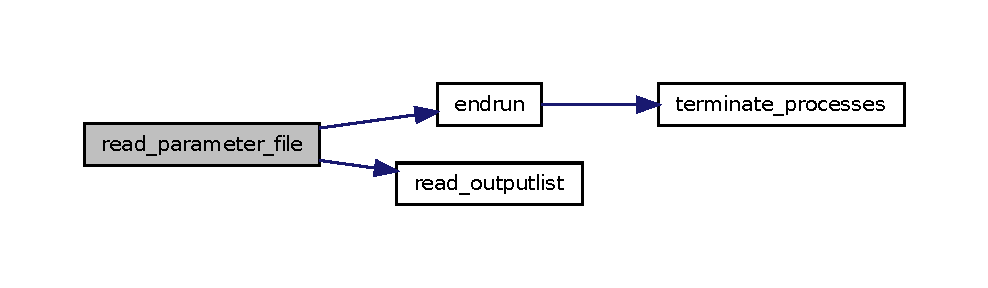
\includegraphics[width=400pt]{begrun_8c_a952eae1977b498c4fdfabed1742a3ba2_cgraph}
\end{center}
\end{figure}




Here is the caller graph for this function:
\nopagebreak
\begin{figure}[H]
\begin{center}
\leavevmode
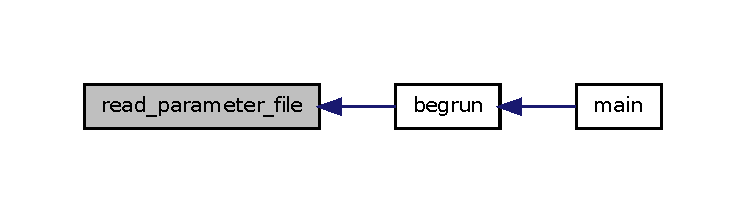
\includegraphics[width=358pt]{begrun_8c_a952eae1977b498c4fdfabed1742a3ba2_icgraph}
\end{center}
\end{figure}


\hypertarget{begrun_8c_acc4d1f5e4e51140090a7ce25ea263b98}{
\index{begrun.c@{begrun.c}!readjust\_\-timebase@{readjust\_\-timebase}}
\index{readjust\_\-timebase@{readjust\_\-timebase}!begrun.c@{begrun.c}}
\subsubsection[{readjust\_\-timebase}]{\setlength{\rightskip}{0pt plus 5cm}void readjust\_\-timebase (
\begin{DoxyParamCaption}
\item[{double}]{ TimeMax\_\-old, }
\item[{double}]{ TimeMax\_\-new}
\end{DoxyParamCaption}
)}}
\label{begrun_8c_acc4d1f5e4e51140090a7ce25ea263b98}
If a restart from restart-\/files is carried out where the TimeMax variable is increased, then the integer timeline needs to be adjusted. The approach taken here is to reduce the resolution of the integer timeline by factors of 2 until the new final time can be reached within TIMEBASE. 

$<$ The simulated timespan is mapped onto the integer interval \mbox{[}0,TIMESPAN\mbox{]}, $\ast$ where TIMESPAN needs to be a power of 2. Note that (1$<$$<$28) corresponds to 2$^\wedge$29 



Definition at line 804 of file begrun.c.



References All, global\_\-data\_\-all\_\-processes::ComovingIntegrationOn, endrun(), NumPart, P, global\_\-data\_\-all\_\-processes::PM\_\-Ti\_\-begstep, global\_\-data\_\-all\_\-processes::PM\_\-Ti\_\-endstep, ThisTask, particle\_\-data::Ti\_\-begstep, global\_\-data\_\-all\_\-processes::Ti\_\-Current, particle\_\-data::Ti\_\-endstep, TIMEBASE, global\_\-data\_\-all\_\-processes::Timebase\_\-interval, global\_\-data\_\-all\_\-processes::TimeBegin, and global\_\-data\_\-all\_\-processes::TimeMax.



Referenced by begrun().




\begin{DoxyCode}
{
  int i;
  long long ti_end;

  if(ThisTask == 0)
    {
      printf("\nAll.TimeMax has been changed in the parameterfile\n");
      printf("Need to adjust integer timeline\n\n\n");
    }

  if(TimeMax_new < TimeMax_old)
    {
      if(ThisTask == 0)
        printf("\nIt is not allowed to reduce All.TimeMax\n\n");
      endrun(556);
    }

  if(All.ComovingIntegrationOn)
    ti_end = log(TimeMax_new / All.TimeBegin) / All.Timebase_interval;
  else
    ti_end = (TimeMax_new - All.TimeBegin) / All.Timebase_interval;

  while(ti_end > TIMEBASE)
    {
      All.Timebase_interval *= 2.0;

      ti_end /= 2;
      All.Ti_Current /= 2;

#ifdef PMGRID
      All.PM_Ti_begstep /= 2;
      All.PM_Ti_endstep /= 2;
#endif

      for(i = 0; i < NumPart; i++)
        {
          P[i].Ti_begstep /= 2;
          P[i].Ti_endstep /= 2;
        }
    }

  All.TimeMax = TimeMax_new;
}
\end{DoxyCode}




Here is the call graph for this function:
\nopagebreak
\begin{figure}[H]
\begin{center}
\leavevmode
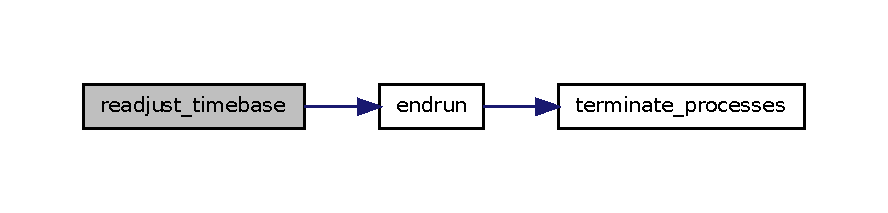
\includegraphics[width=400pt]{begrun_8c_acc4d1f5e4e51140090a7ce25ea263b98_cgraph}
\end{center}
\end{figure}




Here is the caller graph for this function:
\nopagebreak
\begin{figure}[H]
\begin{center}
\leavevmode
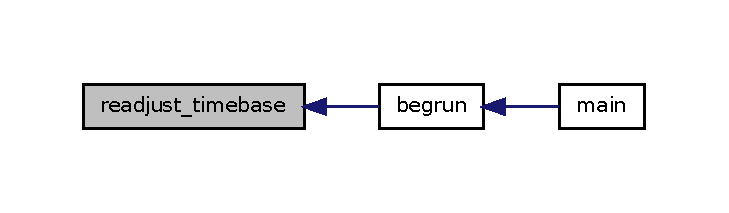
\includegraphics[width=350pt]{begrun_8c_acc4d1f5e4e51140090a7ce25ea263b98_icgraph}
\end{center}
\end{figure}


\hypertarget{begrun_8c_aba986f6be1d66945199c7ea43e5c9610}{
\index{begrun.c@{begrun.c}!set\_\-units@{set\_\-units}}
\index{set\_\-units@{set\_\-units}!begrun.c@{begrun.c}}
\subsubsection[{set\_\-units}]{\setlength{\rightskip}{0pt plus 5cm}void set\_\-units (
\begin{DoxyParamCaption}
\item[{void}]{}
\end{DoxyParamCaption}
)}}
\label{begrun_8c_aba986f6be1d66945199c7ea43e5c9610}
Computes conversion factors between internal code units and the cgs-\/system. 

$<$ Gravitational constant (in cgs units)

$<$ mass fraction of hydrogen, relevant only for radiative cooling

$<$ adiabatic index of simulated gas 



Definition at line 154 of file begrun.c.



References All, BOLTZMANN, global\_\-data\_\-all\_\-processes::G, GRAVITY, global\_\-data\_\-all\_\-processes::GravityConstantInternal, HUBBLE, global\_\-data\_\-all\_\-processes::Hubble, global\_\-data\_\-all\_\-processes::MinEgySpec, global\_\-data\_\-all\_\-processes::MinGasTemp, pow(), PROTONMASS, ThisTask, global\_\-data\_\-all\_\-processes::UnitCoolingRate\_\-in\_\-cgs, global\_\-data\_\-all\_\-processes::UnitDensity\_\-in\_\-cgs, global\_\-data\_\-all\_\-processes::UnitEnergy\_\-in\_\-cgs, global\_\-data\_\-all\_\-processes::UnitLength\_\-in\_\-cm, global\_\-data\_\-all\_\-processes::UnitMass\_\-in\_\-g, global\_\-data\_\-all\_\-processes::UnitPressure\_\-in\_\-cgs, global\_\-data\_\-all\_\-processes::UnitTime\_\-in\_\-Megayears, global\_\-data\_\-all\_\-processes::UnitTime\_\-in\_\-s, and global\_\-data\_\-all\_\-processes::UnitVelocity\_\-in\_\-cm\_\-per\_\-s.



Referenced by begrun().




\begin{DoxyCode}
{
  double meanweight;

  All.UnitTime_in_s = All.UnitLength_in_cm / All.UnitVelocity_in_cm_per_s;
  All.UnitTime_in_Megayears = All.UnitTime_in_s / SEC_PER_MEGAYEAR;

  if(All.GravityConstantInternal == 0)
    All.G = GRAVITY / pow(All.UnitLength_in_cm, 3) * All.UnitMass_in_g * pow(All.
      UnitTime_in_s, 2);
  else
    All.G = All.GravityConstantInternal;

  All.UnitDensity_in_cgs = All.UnitMass_in_g / pow(All.UnitLength_in_cm, 3);
  All.UnitPressure_in_cgs = All.UnitMass_in_g / All.UnitLength_in_cm / pow(All.
      UnitTime_in_s, 2);
  All.UnitCoolingRate_in_cgs = All.UnitPressure_in_cgs / All.UnitTime_in_s;
  All.UnitEnergy_in_cgs = All.UnitMass_in_g * pow(All.UnitLength_in_cm, 2) / pow(
      All.UnitTime_in_s, 2);

  /* convert some physical input parameters to internal units */

  All.Hubble = HUBBLE * All.UnitTime_in_s;

  if(ThisTask == 0)
    {
      printf("\nHubble (internal units) = %g\n", All.Hubble);
      printf("G (internal units) = %g\n", All.G);
      printf("UnitMass_in_g = %g \n", All.UnitMass_in_g);
      printf("UnitTime_in_s = %g \n", All.UnitTime_in_s);
      printf("UnitVelocity_in_cm_per_s = %g \n", All.UnitVelocity_in_cm_per_s);
      printf("UnitDensity_in_cgs = %g \n", All.UnitDensity_in_cgs);
      printf("UnitEnergy_in_cgs = %g \n", All.UnitEnergy_in_cgs);
      printf("\n");
    }

  meanweight = 4.0 / (1 + 3 * HYDROGEN_MASSFRAC);       /* note: we assume neutra
      l gas here */

#ifdef ISOTHERM_EQS
  All.MinEgySpec = 0;
#else
  All.MinEgySpec = 1 / meanweight * (1.0 / GAMMA_MINUS1) * (BOLTZMANN / 
      PROTONMASS) * All.MinGasTemp;
  All.MinEgySpec *= All.UnitMass_in_g / All.UnitEnergy_in_cgs;
#endif

}
\end{DoxyCode}




Here is the call graph for this function:
\nopagebreak
\begin{figure}[H]
\begin{center}
\leavevmode
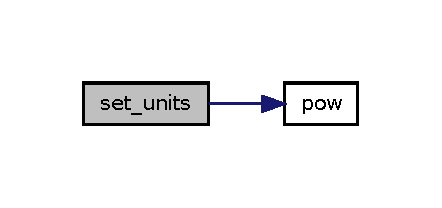
\includegraphics[width=212pt]{begrun_8c_aba986f6be1d66945199c7ea43e5c9610_cgraph}
\end{center}
\end{figure}




Here is the caller graph for this function:
\nopagebreak
\begin{figure}[H]
\begin{center}
\leavevmode
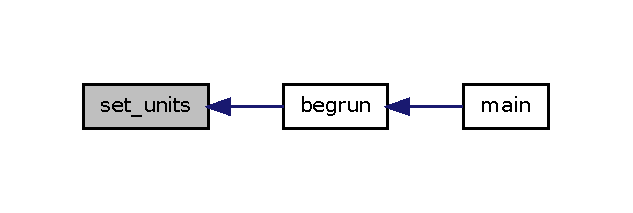
\includegraphics[width=304pt]{begrun_8c_aba986f6be1d66945199c7ea43e5c9610_icgraph}
\end{center}
\end{figure}



\hypertarget{density_8c}{\section{density.\-c \-File \-Reference}
\label{density_8c}\index{density.\-c@{density.\-c}}
}


\-S\-P\-H density computation and smoothing length determination.  


{\ttfamily \#include $<$stdio.\-h$>$}\*
{\ttfamily \#include $<$stdlib.\-h$>$}\*
{\ttfamily \#include $<$string.\-h$>$}\*
{\ttfamily \#include $<$math.\-h$>$}\*
{\ttfamily \#include $<$mpi.\-h$>$}\*
{\ttfamily \#include \char`\"{}allvars.\-h\char`\"{}}\*
{\ttfamily \#include \char`\"{}proto.\-h\char`\"{}}\*
\-Include dependency graph for density.\-c\-:
\nopagebreak
\begin{figure}[H]
\begin{center}
\leavevmode
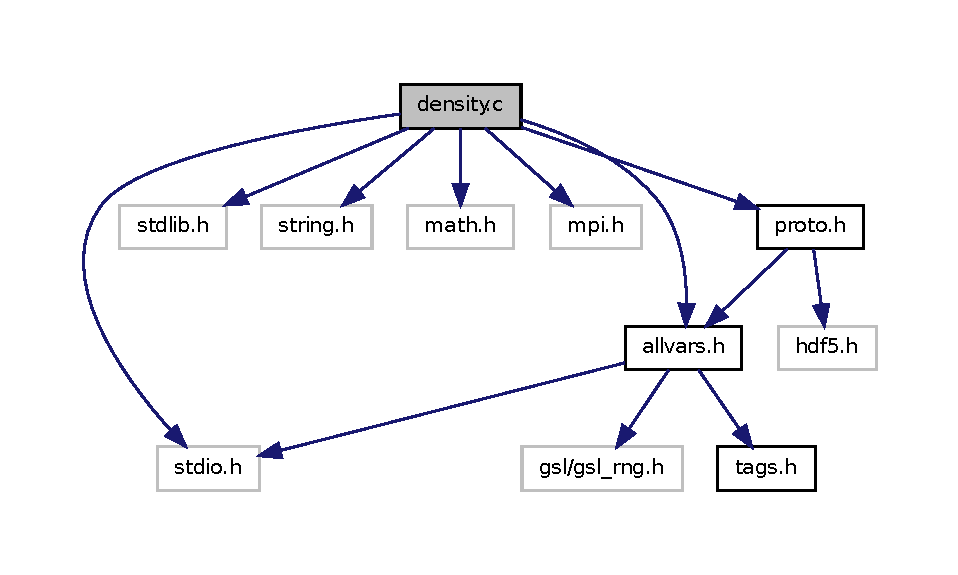
\includegraphics[width=350pt]{density_8c__incl}
\end{center}
\end{figure}
\subsection*{\-Defines}
\begin{DoxyCompactItemize}
\item 
\#define \hyperlink{density_8c_a5c5328b307b005e6682669279878cef0}{box\-Size\-\_\-\-X}~\hyperlink{ngb_8c_ac9067960018a06b81c117434c01f19cc}{box\-Size}
\item 
\#define \hyperlink{density_8c_a0ecceb71797a529fb6f2b8c47b51686c}{box\-Half\-\_\-\-X}~\hyperlink{ngb_8c_af62571c97dc75a691aeafead0528b369}{box\-Half}
\item 
\#define \hyperlink{density_8c_ab0db73a31e08d33d840e28651e3cf610}{box\-Size\-\_\-\-Y}~\hyperlink{ngb_8c_ac9067960018a06b81c117434c01f19cc}{box\-Size}
\item 
\#define \hyperlink{density_8c_a59f20d7decc2bdfedcaafb70ef23df0e}{box\-Half\-\_\-\-Y}~\hyperlink{ngb_8c_af62571c97dc75a691aeafead0528b369}{box\-Half}
\item 
\#define \hyperlink{density_8c_a8a97a1c456bdd396791c84c370f0aa18}{box\-Size\-\_\-\-Z}~\hyperlink{ngb_8c_ac9067960018a06b81c117434c01f19cc}{box\-Size}
\item 
\#define \hyperlink{density_8c_a34e9d5d079320cbfc0576d26f58d2fe7}{box\-Half\-\_\-\-Z}~\hyperlink{ngb_8c_af62571c97dc75a691aeafead0528b369}{box\-Half}
\end{DoxyCompactItemize}
\subsection*{\-Functions}
\begin{DoxyCompactItemize}
\item 
void \hyperlink{density_8c_ad86cdeb9e3bfbe9af379ac9f7daf194c}{density} (void)
\item 
void \hyperlink{density_8c_a4e6b32342a24a33518b6ae8723809749}{density\-\_\-evaluate} (int target, int mode)
\item 
int \hyperlink{density_8c_ab6453dd0ac2ecf2478b1208374e68ae1}{dens\-\_\-compare\-\_\-key} (const void $\ast$a, const void $\ast$b)
\end{DoxyCompactItemize}
\subsection*{\-Variables}
\begin{DoxyCompactItemize}
\item 
static double \hyperlink{density_8c_ac9067960018a06b81c117434c01f19cc}{box\-Size}
\item 
static double \hyperlink{density_8c_af62571c97dc75a691aeafead0528b369}{box\-Half}
\end{DoxyCompactItemize}


\subsection{\-Detailed \-Description}
\-S\-P\-H density computation and smoothing length determination. \-This file contains the \char`\"{}first S\-P\-H loop\char`\"{}, where the \-S\-P\-H densities and some auxiliary quantities are computed. \-If the number of neighbours obtained falls outside the target range, the correct smoothing length is determined iteratively, if needed. 

\-Definition in file \hyperlink{density_8c_source}{density.\-c}.



\subsection{\-Define \-Documentation}
\hypertarget{density_8c_a0ecceb71797a529fb6f2b8c47b51686c}{\index{density.\-c@{density.\-c}!box\-Half\-\_\-\-X@{box\-Half\-\_\-\-X}}
\index{box\-Half\-\_\-\-X@{box\-Half\-\_\-\-X}!density.c@{density.\-c}}
\subsubsection[{box\-Half\-\_\-\-X}]{\setlength{\rightskip}{0pt plus 5cm}\#define {\bf box\-Half\-\_\-\-X}~{\bf box\-Half}}}\label{density_8c_a0ecceb71797a529fb6f2b8c47b51686c}


\-Definition at line 28 of file density.\-c.



\-Referenced by density(), and density\-\_\-evaluate().

\hypertarget{density_8c_a59f20d7decc2bdfedcaafb70ef23df0e}{\index{density.\-c@{density.\-c}!box\-Half\-\_\-\-Y@{box\-Half\-\_\-\-Y}}
\index{box\-Half\-\_\-\-Y@{box\-Half\-\_\-\-Y}!density.c@{density.\-c}}
\subsubsection[{box\-Half\-\_\-\-Y}]{\setlength{\rightskip}{0pt plus 5cm}\#define {\bf box\-Half\-\_\-\-Y}~{\bf box\-Half}}}\label{density_8c_a59f20d7decc2bdfedcaafb70ef23df0e}


\-Definition at line 34 of file density.\-c.



\-Referenced by density(), and density\-\_\-evaluate().

\hypertarget{density_8c_a34e9d5d079320cbfc0576d26f58d2fe7}{\index{density.\-c@{density.\-c}!box\-Half\-\_\-\-Z@{box\-Half\-\_\-\-Z}}
\index{box\-Half\-\_\-\-Z@{box\-Half\-\_\-\-Z}!density.c@{density.\-c}}
\subsubsection[{box\-Half\-\_\-\-Z}]{\setlength{\rightskip}{0pt plus 5cm}\#define {\bf box\-Half\-\_\-\-Z}~{\bf box\-Half}}}\label{density_8c_a34e9d5d079320cbfc0576d26f58d2fe7}


\-Definition at line 40 of file density.\-c.



\-Referenced by density(), and density\-\_\-evaluate().

\hypertarget{density_8c_a5c5328b307b005e6682669279878cef0}{\index{density.\-c@{density.\-c}!box\-Size\-\_\-\-X@{box\-Size\-\_\-\-X}}
\index{box\-Size\-\_\-\-X@{box\-Size\-\_\-\-X}!density.c@{density.\-c}}
\subsubsection[{box\-Size\-\_\-\-X}]{\setlength{\rightskip}{0pt plus 5cm}\#define {\bf box\-Size\-\_\-\-X}~{\bf box\-Size}}}\label{density_8c_a5c5328b307b005e6682669279878cef0}


\-Definition at line 27 of file density.\-c.



\-Referenced by density(), and density\-\_\-evaluate().

\hypertarget{density_8c_ab0db73a31e08d33d840e28651e3cf610}{\index{density.\-c@{density.\-c}!box\-Size\-\_\-\-Y@{box\-Size\-\_\-\-Y}}
\index{box\-Size\-\_\-\-Y@{box\-Size\-\_\-\-Y}!density.c@{density.\-c}}
\subsubsection[{box\-Size\-\_\-\-Y}]{\setlength{\rightskip}{0pt plus 5cm}\#define {\bf box\-Size\-\_\-\-Y}~{\bf box\-Size}}}\label{density_8c_ab0db73a31e08d33d840e28651e3cf610}


\-Definition at line 33 of file density.\-c.



\-Referenced by density(), and density\-\_\-evaluate().

\hypertarget{density_8c_a8a97a1c456bdd396791c84c370f0aa18}{\index{density.\-c@{density.\-c}!box\-Size\-\_\-\-Z@{box\-Size\-\_\-\-Z}}
\index{box\-Size\-\_\-\-Z@{box\-Size\-\_\-\-Z}!density.c@{density.\-c}}
\subsubsection[{box\-Size\-\_\-\-Z}]{\setlength{\rightskip}{0pt plus 5cm}\#define {\bf box\-Size\-\_\-\-Z}~{\bf box\-Size}}}\label{density_8c_a8a97a1c456bdd396791c84c370f0aa18}


\-Definition at line 39 of file density.\-c.



\-Referenced by density(), and density\-\_\-evaluate().



\subsection{\-Function \-Documentation}
\hypertarget{density_8c_ab6453dd0ac2ecf2478b1208374e68ae1}{\index{density.\-c@{density.\-c}!dens\-\_\-compare\-\_\-key@{dens\-\_\-compare\-\_\-key}}
\index{dens\-\_\-compare\-\_\-key@{dens\-\_\-compare\-\_\-key}!density.c@{density.\-c}}
\subsubsection[{dens\-\_\-compare\-\_\-key}]{\setlength{\rightskip}{0pt plus 5cm}int {\bf dens\-\_\-compare\-\_\-key} (
\begin{DoxyParamCaption}
\item[{const void $\ast$}]{a, }
\item[{const void $\ast$}]{b}
\end{DoxyParamCaption}
)}}\label{density_8c_ab6453dd0ac2ecf2478b1208374e68ae1}
\-This routine is a comparison kernel used in a sort routine to group particles that are exported to the same processor. 

\-Definition at line 607 of file density.\-c.



\-Referenced by density().


\begin{DoxyCode}
{
  if(((struct densdata_in *) a)->Task < (((struct densdata_in *) b)->Task))
    return -1;

  if(((struct densdata_in *) a)->Task > (((struct densdata_in *) b)->Task))
    return +1;

  return 0;
}
\end{DoxyCode}


\-Here is the caller graph for this function\-:
\nopagebreak
\begin{figure}[H]
\begin{center}
\leavevmode
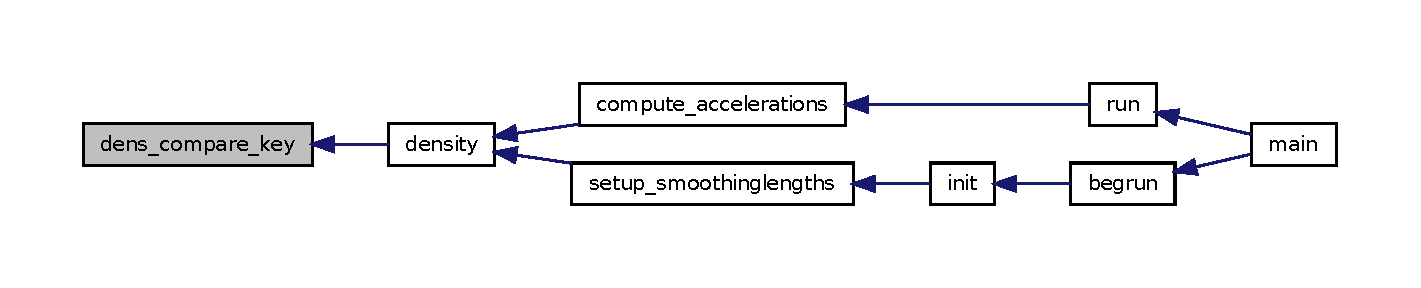
\includegraphics[width=350pt]{density_8c_ab6453dd0ac2ecf2478b1208374e68ae1_icgraph}
\end{center}
\end{figure}


\hypertarget{density_8c_ad86cdeb9e3bfbe9af379ac9f7daf194c}{\index{density.\-c@{density.\-c}!density@{density}}
\index{density@{density}!density.c@{density.\-c}}
\subsubsection[{density}]{\setlength{\rightskip}{0pt plus 5cm}void {\bf density} (
\begin{DoxyParamCaption}
\item[{void}]{}
\end{DoxyParamCaption}
)}}\label{density_8c_ad86cdeb9e3bfbe9af379ac9f7daf194c}
\-This function computes the local density for each active \-S\-P\-H particle, the number of neighbours in the current smoothing radius, and the divergence and curl of the velocity field. \-The pressure is updated as well. \-If a particle with its smoothing region is fully inside the local domain, it is not exported to the other processors. \-The function also detects particles that have a number of neighbours outside the allowed tolerance range. \-For these particles, the smoothing length is adjusted accordingly, and the density computation is executed again. \-Note that the smoothing length is not allowed to fall below the lower bound set by \-Min\-Gas\-Hsml. $<$ \-For 3\-D-\/normalized kernel

$<$ adiabatic index of simulated gas

$<$ maxmimum number of steps for \-S\-P\-H neighbour iteration

$<$ \-For 3\-D-\/normalized kernel

$<$ \-For 3\-D-\/normalized kernel

$<$ maxmimum number of steps for \-S\-P\-H neighbour iteration 

\-Definition at line 56 of file density.\-c.



\-References \-All, box\-Half, box\-Half\-\_\-\-X, box\-Half\-\_\-\-Y, box\-Half\-\_\-\-Z, box\-Size, box\-Size\-\_\-\-X, box\-Size\-\_\-\-Y, box\-Size\-\_\-\-Z, dens\-\_\-compare\-\_\-key(), \-Dens\-Data\-Get, \-Dens\-Data\-In, \-Dens\-Data\-Partial\-Result, \-Dens\-Data\-Result, density\-\_\-evaluate(), dmax(), endrun(), \-Exportflag, \-N\-\_\-gas, \-N\-Task, \-Num\-Part, \-Num\-Sph\-Update, \-P, pow(), \-P\-Task, second(), \-Sph\-P, \-T\-A\-G\-\_\-\-D\-E\-N\-S\-\_\-\-A, \-T\-A\-G\-\_\-\-D\-E\-N\-S\-\_\-\-B, \-This\-Task, and timediff().



\-Referenced by compute\-\_\-accelerations(), and setup\-\_\-smoothinglengths().


\begin{DoxyCode}
{
  long long ntot, ntotleft;
  int *noffset, *nbuffer, *nsend, *nsend_local, *numlist, *ndonelist;
  int i, j, n, ndone, npleft, maxfill, source, iter = 0;
  int level, ngrp, sendTask, recvTask, place, nexport;
  double dt_entr, tstart, tend, tstart_ngb = 0, tend_ngb = 0;
  double sumt, sumcomm, timengb, sumtimengb;
  double timecomp = 0, timeimbalance = 0, timecommsumm = 0, sumimbalance;
  MPI_Status status;

#ifdef PERIODIC
  boxSize = All.BoxSize;
  boxHalf = 0.5 * All.BoxSize;
#ifdef LONG_X
  boxHalf_X = boxHalf * LONG_X;
  boxSize_X = boxSize * LONG_X;
#endif
#ifdef LONG_Y
  boxHalf_Y = boxHalf * LONG_Y;
  boxSize_Y = boxSize * LONG_Y;
#endif
#ifdef LONG_Z
  boxHalf_Z = boxHalf * LONG_Z;
  boxSize_Z = boxSize * LONG_Z;
#endif
#endif


  noffset = malloc(sizeof(int) * NTask);        /* offsets of bunches in common
       list */
  nbuffer = malloc(sizeof(int) * NTask);
  nsend_local = malloc(sizeof(int) * NTask);
  nsend = malloc(sizeof(int) * NTask * NTask);
  ndonelist = malloc(sizeof(int) * NTask);

  for(n = 0, NumSphUpdate = 0; n < N_gas; n++)
    {
      SphP[n].Left = SphP[n].Right = 0;

      if(P[n].Ti_endstep == All.Ti_Current)
        NumSphUpdate++;
    }

  numlist = malloc(NTask * sizeof(int) * NTask);
  MPI_Allgather(&NumSphUpdate, 1, MPI_INT, numlist, 1, MPI_INT, MPI_COMM_WORLD)
      ;
  for(i = 0, ntot = 0; i < NTask; i++)
    ntot += numlist[i];
  free(numlist);



  /* we will repeat the whole thing for those particles where we didn't
   * find enough neighbours
   */
  do
    {
      i = 0;                    /* beginn with this index */
      ntotleft = ntot;          /* particles left for all tasks together */

      while(ntotleft > 0)
        {
          for(j = 0; j < NTask; j++)
            nsend_local[j] = 0;

          /* do local particles and prepare export list */
          tstart = second();
          for(nexport = 0, ndone = 0; i < N_gas && nexport < All.
      BunchSizeDensity - NTask; i++)
            if(P[i].Ti_endstep == All.Ti_Current)
              {
                ndone++;

                for(j = 0; j < NTask; j++)
                  Exportflag[j] = 0;

                density_evaluate(i, 0);

                for(j = 0; j < NTask; j++)
                  {
                    if(Exportflag[j])
                      {
                        DensDataIn[nexport].Pos[0] = P[i].Pos[0];
                        DensDataIn[nexport].Pos[1] = P[i].Pos[1];
                        DensDataIn[nexport].Pos[2] = P[i].Pos[2];
                        DensDataIn[nexport].Vel[0] = SphP[i].VelPred[0];
                        DensDataIn[nexport].Vel[1] = SphP[i].VelPred[1];
                        DensDataIn[nexport].Vel[2] = SphP[i].VelPred[2];
                        DensDataIn[nexport].Hsml = SphP[i].Hsml;
                        DensDataIn[nexport].Index = i;
                        DensDataIn[nexport].Task = j;
                        nexport++;
                        nsend_local[j]++;
                      }
                  }
              }
          tend = second();
          timecomp += timediff(tstart, tend);

          qsort(DensDataIn, nexport, sizeof(struct densdata_in), 
      dens_compare_key);

          for(j = 1, noffset[0] = 0; j < NTask; j++)
            noffset[j] = noffset[j - 1] + nsend_local[j - 1];

          tstart = second();

          MPI_Allgather(nsend_local, NTask, MPI_INT, nsend, NTask, MPI_INT, 
      MPI_COMM_WORLD);

          tend = second();
          timeimbalance += timediff(tstart, tend);


          /* now do the particles that need to be exported */

          for(level = 1; level < (1 << PTask); level++)
            {
              tstart = second();
              for(j = 0; j < NTask; j++)
                nbuffer[j] = 0;
              for(ngrp = level; ngrp < (1 << PTask); ngrp++)
                {
                  maxfill = 0;
                  for(j = 0; j < NTask; j++)
                    {
                      if((j ^ ngrp) < NTask)
                        if(maxfill < nbuffer[j] + nsend[(j ^ ngrp) * NTask + j]
      )
                          maxfill = nbuffer[j] + nsend[(j ^ ngrp) * NTask + j];
                    }
                  if(maxfill >= All.BunchSizeDensity)
                    break;

                  sendTask = ThisTask;
                  recvTask = ThisTask ^ ngrp;

                  if(recvTask < NTask)
                    {
                      if(nsend[ThisTask * NTask + recvTask] > 0 || nsend[
      recvTask * NTask + ThisTask] > 0)
                        {
                          /* get the particles */
                          MPI_Sendrecv(&DensDataIn[noffset[recvTask]],
                                       nsend_local[recvTask] * sizeof(struct 
      densdata_in), MPI_BYTE,
                                       recvTask, TAG_DENS_A,
                                       &DensDataGet[nbuffer[ThisTask]],
                                       nsend[recvTask * NTask + ThisTask] * 
      sizeof(struct densdata_in),
                                       MPI_BYTE, recvTask, TAG_DENS_A, 
      MPI_COMM_WORLD, &status);
                        }
                    }

                  for(j = 0; j < NTask; j++)
                    if((j ^ ngrp) < NTask)
                      nbuffer[j] += nsend[(j ^ ngrp) * NTask + j];
                }
              tend = second();
              timecommsumm += timediff(tstart, tend);


              tstart = second();
              for(j = 0; j < nbuffer[ThisTask]; j++)
                density_evaluate(j, 1);
              tend = second();
              timecomp += timediff(tstart, tend);

              /* do a block to explicitly measure imbalance */
              tstart = second();
              MPI_Barrier(MPI_COMM_WORLD);
              tend = second();
              timeimbalance += timediff(tstart, tend);

              /* get the result */
              tstart = second();
              for(j = 0; j < NTask; j++)
                nbuffer[j] = 0;
              for(ngrp = level; ngrp < (1 << PTask); ngrp++)
                {
                  maxfill = 0;
                  for(j = 0; j < NTask; j++)
                    {
                      if((j ^ ngrp) < NTask)
                        if(maxfill < nbuffer[j] + nsend[(j ^ ngrp) * NTask + j]
      )
                          maxfill = nbuffer[j] + nsend[(j ^ ngrp) * NTask + j];
                    }
                  if(maxfill >= All.BunchSizeDensity)
                    break;

                  sendTask = ThisTask;
                  recvTask = ThisTask ^ ngrp;

                  if(recvTask < NTask)
                    {
                      if(nsend[ThisTask * NTask + recvTask] > 0 || nsend[
      recvTask * NTask + ThisTask] > 0)
                        {
                          /* send the results */
                          MPI_Sendrecv(&DensDataResult[nbuffer[ThisTask]],
                                       nsend[recvTask * NTask + ThisTask] * 
      sizeof(struct densdata_out),
                                       MPI_BYTE, recvTask, TAG_DENS_B,
                                       &DensDataPartialResult[noffset[recvTask]
      ],
                                       nsend_local[recvTask] * sizeof(struct 
      densdata_out),
                                       MPI_BYTE, recvTask, TAG_DENS_B, 
      MPI_COMM_WORLD, &status);

                          /* add the result to the particles */
                          for(j = 0; j < nsend_local[recvTask]; j++)
                            {
                              source = j + noffset[recvTask];
                              place = DensDataIn[source].Index;

                              SphP[place].NumNgb += DensDataPartialResult[
      source].Ngb;
                              SphP[place].Density += DensDataPartialResult[
      source].Rho;
                              SphP[place].DivVel += DensDataPartialResult[
      source].Div;

                              SphP[place].DhsmlDensityFactor += 
      DensDataPartialResult[source].DhsmlDensity;

                              SphP[place].Rot[0] += DensDataPartialResult[
      source].Rot[0];
                              SphP[place].Rot[1] += DensDataPartialResult[
      source].Rot[1];
                              SphP[place].Rot[2] += DensDataPartialResult[
      source].Rot[2];
                            }
                        }
                    }

                  for(j = 0; j < NTask; j++)
                    if((j ^ ngrp) < NTask)
                      nbuffer[j] += nsend[(j ^ ngrp) * NTask + j];
                }
              tend = second();
              timecommsumm += timediff(tstart, tend);

              level = ngrp - 1;
            }

          MPI_Allgather(&ndone, 1, MPI_INT, ndonelist, 1, MPI_INT, 
      MPI_COMM_WORLD);
          for(j = 0; j < NTask; j++)
            ntotleft -= ndonelist[j];
        }



      /* do final operations on results */
      tstart = second();
      for(i = 0, npleft = 0; i < N_gas; i++)
        {
          if(P[i].Ti_endstep == All.Ti_Current)
            {
              {
                SphP[i].DhsmlDensityFactor =
                  1 / (1 + SphP[i].Hsml * SphP[i].DhsmlDensityFactor / (NUMDIMS
       * SphP[i].Density));

                SphP[i].CurlVel = sqrt(SphP[i].Rot[0] * SphP[i].Rot[0] +
                                       SphP[i].Rot[1] * SphP[i].Rot[1] +
                                       SphP[i].Rot[2] * SphP[i].Rot[2]) / SphP[
      i].Density;

                SphP[i].DivVel /= SphP[i].Density;

                dt_entr = (All.Ti_Current - (P[i].Ti_begstep + P[i].Ti_endstep)
       / 2) * All.Timebase_interval;

                SphP[i].Pressure =
                  (SphP[i].Entropy + SphP[i].DtEntropy * dt_entr) * pow(SphP[i]
      .Density, GAMMA);
              }


              /* now check whether we had enough neighbours */

              if(SphP[i].NumNgb < (All.DesNumNgb - All.MaxNumNgbDeviation) ||
                 (SphP[i].NumNgb > (All.DesNumNgb + All.MaxNumNgbDeviation)
                  && SphP[i].Hsml > (1.01 * All.MinGasHsml)))
                {
                  /* need to redo this particle */
                  npleft++;

                  if(SphP[i].Left > 0 && SphP[i].Right > 0)
                    if((SphP[i].Right - SphP[i].Left) < 1.0e-3 * SphP[i].Left)
                      {
                        /* this one should be ok */
                        npleft--;
                        P[i].Ti_endstep = -P[i].Ti_endstep - 1; /* Mark as
       inactive */
                        continue;
                      }

                  if(SphP[i].NumNgb < (All.DesNumNgb - All.MaxNumNgbDeviation))
                    SphP[i].Left = dmax(SphP[i].Hsml, SphP[i].Left);
                  else
                    {
                      if(SphP[i].Right != 0)
                        {
                          if(SphP[i].Hsml < SphP[i].Right)
                            SphP[i].Right = SphP[i].Hsml;
                        }
                      else
                        SphP[i].Right = SphP[i].Hsml;
                    }

                  if(iter >= MAXITER - 10)
                    {
                      printf
                        ("i=%d task=%d ID=%d Hsml=%g Left=%g Right=%g Ngbs=%g
       Right-Left=%g\n   pos=(%g|%g|%g)\n",
                         i, ThisTask, (int) P[i].ID, SphP[i].Hsml, SphP[i].Left
      , SphP[i].Right,
                         (float) SphP[i].NumNgb, SphP[i].Right - SphP[i].Left, P
      [i].Pos[0], P[i].Pos[1],
                         P[i].Pos[2]);
                      fflush(stdout);
                    }

                  if(SphP[i].Right > 0 && SphP[i].Left > 0)
                    SphP[i].Hsml = pow(0.5 * (pow(SphP[i].Left, 3) + pow(SphP[i
      ].Right, 3)), 1.0 / 3);
                  else
                    {
                      if(SphP[i].Right == 0 && SphP[i].Left == 0)
                        endrun(8188);   /* can't occur */

                      if(SphP[i].Right == 0 && SphP[i].Left > 0)
                        {
                          if(P[i].Type == 0 && fabs(SphP[i].NumNgb - All.
      DesNumNgb) < 0.5 * All.DesNumNgb)
                            {
                              SphP[i].Hsml *=
                                1 - (SphP[i].NumNgb -
                                     All.DesNumNgb) / (NUMDIMS * SphP[i].NumNgb
      ) * SphP[i].DhsmlDensityFactor;
                            }
                          else
                            SphP[i].Hsml *= 1.26;
                        }

                      if(SphP[i].Right > 0 && SphP[i].Left == 0)
                        {
                          if(P[i].Type == 0 && fabs(SphP[i].NumNgb - All.
      DesNumNgb) < 0.5 * All.DesNumNgb)
                            {
                              SphP[i].Hsml *=
                                1 - (SphP[i].NumNgb -
                                     All.DesNumNgb) / (NUMDIMS * SphP[i].NumNgb
      ) * SphP[i].DhsmlDensityFactor;
                            }
                          else
                            SphP[i].Hsml /= 1.26;
                        }
                    }

                  if(SphP[i].Hsml < All.MinGasHsml)
                    SphP[i].Hsml = All.MinGasHsml;
                }
              else
                P[i].Ti_endstep = -P[i].Ti_endstep - 1; /* Mark as inactive */
            }
        }
      tend = second();
      timecomp += timediff(tstart, tend);


      numlist = malloc(NTask * sizeof(int) * NTask);
      MPI_Allgather(&npleft, 1, MPI_INT, numlist, 1, MPI_INT, MPI_COMM_WORLD);
      for(i = 0, ntot = 0; i < NTask; i++)
        ntot += numlist[i];
      free(numlist);

      if(ntot > 0)
        {
          if(iter == 0)
            tstart_ngb = second();

          iter++;

          if(iter > 0 && ThisTask == 0)
            {
              printf("ngb iteration %d: need to repeat for %d%09d particles.\n"
      , iter,
                     (int) (ntot / 1000000000), (int) (ntot % 1000000000));
              fflush(stdout);
            }

          if(iter > MAXITER)
            {
              printf("failed to converge in neighbour iteration in density()\n"
      );
              fflush(stdout);
              endrun(1155);
            }
        }
      else
        tend_ngb = second();
    }
  while(ntot > 0);


  /* mark as active again */
  for(i = 0; i < NumPart; i++)
    if(P[i].Ti_endstep < 0)
      P[i].Ti_endstep = -P[i].Ti_endstep - 1;

  free(ndonelist);
  free(nsend);
  free(nsend_local);
  free(nbuffer);
  free(noffset);


  /* collect some timing information */
  if(iter > 0)
    timengb = timediff(tstart_ngb, tend_ngb);
  else
    timengb = 0;

  MPI_Reduce(&timengb, &sumtimengb, 1, MPI_DOUBLE, MPI_SUM, 0, MPI_COMM_WORLD);
  MPI_Reduce(&timecomp, &sumt, 1, MPI_DOUBLE, MPI_SUM, 0, MPI_COMM_WORLD);
  MPI_Reduce(&timecommsumm, &sumcomm, 1, MPI_DOUBLE, MPI_SUM, 0, MPI_COMM_WORLD
      );
  MPI_Reduce(&timeimbalance, &sumimbalance, 1, MPI_DOUBLE, MPI_SUM, 0, 
      MPI_COMM_WORLD);

  if(ThisTask == 0)
    {
      All.CPU_HydCompWalk += sumt / NTask;
      All.CPU_HydCommSumm += sumcomm / NTask;
      All.CPU_HydImbalance += sumimbalance / NTask;
      All.CPU_EnsureNgb += sumtimengb / NTask;
    }
}
\end{DoxyCode}


\-Here is the call graph for this function\-:
\nopagebreak
\begin{figure}[H]
\begin{center}
\leavevmode
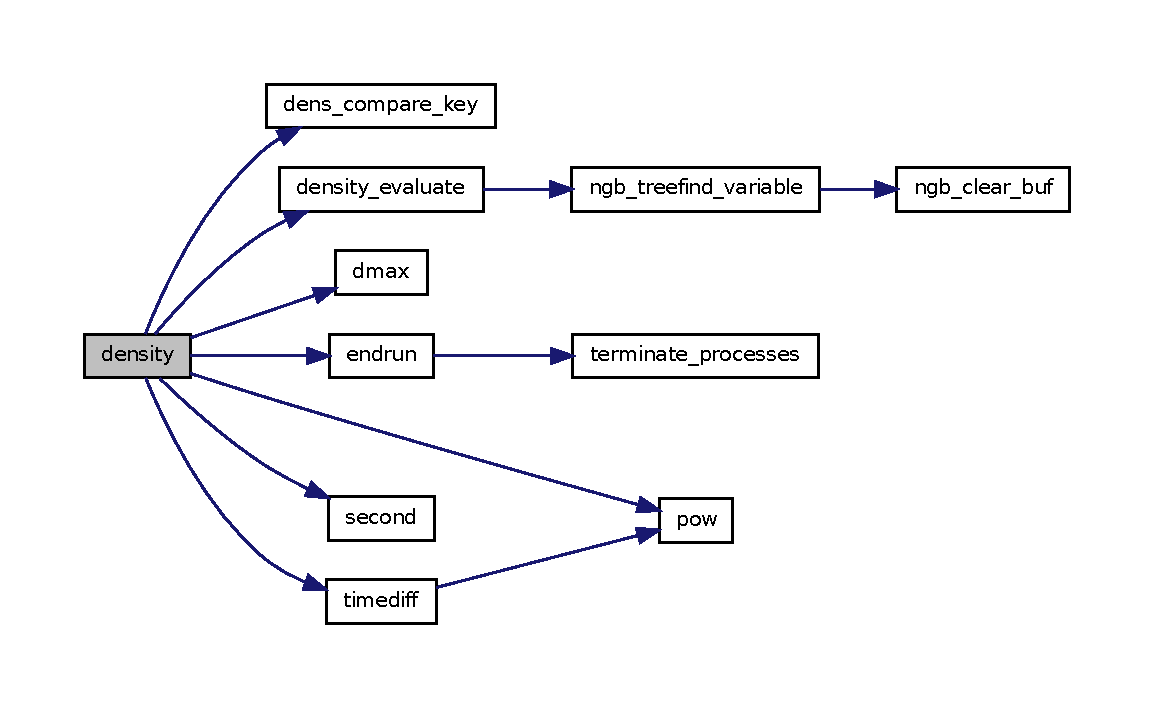
\includegraphics[width=350pt]{density_8c_ad86cdeb9e3bfbe9af379ac9f7daf194c_cgraph}
\end{center}
\end{figure}




\-Here is the caller graph for this function\-:
\nopagebreak
\begin{figure}[H]
\begin{center}
\leavevmode
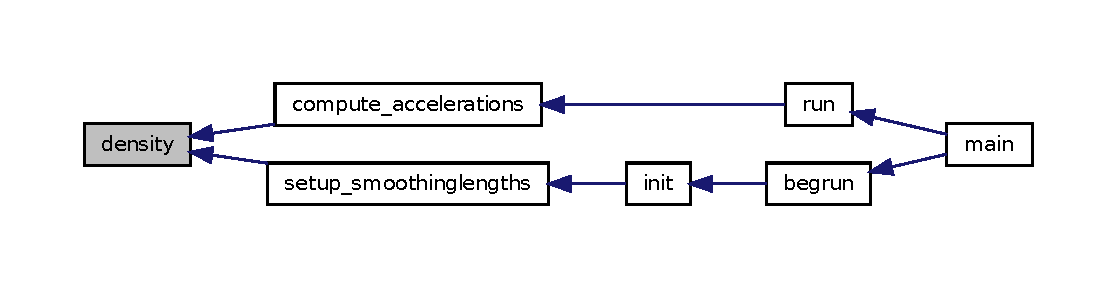
\includegraphics[width=350pt]{density_8c_ad86cdeb9e3bfbe9af379ac9f7daf194c_icgraph}
\end{center}
\end{figure}


\hypertarget{density_8c_a4e6b32342a24a33518b6ae8723809749}{\index{density.\-c@{density.\-c}!density\-\_\-evaluate@{density\-\_\-evaluate}}
\index{density\-\_\-evaluate@{density\-\_\-evaluate}!density.c@{density.\-c}}
\subsubsection[{density\-\_\-evaluate}]{\setlength{\rightskip}{0pt plus 5cm}void {\bf density\-\_\-evaluate} (
\begin{DoxyParamCaption}
\item[{int}]{target, }
\item[{int}]{mode}
\end{DoxyParamCaption}
)}}\label{density_8c_a4e6b32342a24a33518b6ae8723809749}
\-This function represents the core of the \-S\-P\-H density computation. \-The target particle may either be local, or reside in the communication buffer. $<$ \-Coefficients for \-S\-P\-H spline kernel and its derivative

$<$ \-Coefficient for kernel normalization. \-Note\-: 4.\-0/3 $\ast$ \-P\-I = 4.\-188790204786

$<$ \-For 3\-D-\/normalized kernel 

\-Definition at line 467 of file density.\-c.



\-References \-All, box\-Half\-\_\-\-X, box\-Half\-\_\-\-Y, box\-Half\-\_\-\-Z, box\-Size\-\_\-\-X, box\-Size\-\_\-\-Y, box\-Size\-\_\-\-Z, \-Dens\-Data\-Get, \-Dens\-Data\-Result, ngb\-\_\-treefind\-\_\-variable(), \-Ngblist, \-P, and \-Sph\-P.



\-Referenced by density().


\begin{DoxyCode}
{
  int j, n, startnode, numngb, numngb_inbox;
  double h, h2, fac, hinv, hinv3, hinv4;
  double rho, divv, wk, dwk;
  double dx, dy, dz, r, r2, u, mass_j;
  double dvx, dvy, dvz, rotv[3];
  double weighted_numngb, dhsmlrho;
  FLOAT *pos, *vel;

  if(mode == 0)
    {
      pos = P[target].Pos;
      vel = SphP[target].VelPred;
      h = SphP[target].Hsml;
    }
  else
    {
      pos = DensDataGet[target].Pos;
      vel = DensDataGet[target].Vel;
      h = DensDataGet[target].Hsml;
    }

  h2 = h * h;
  hinv = 1.0 / h;
#ifndef  TWODIMS
  hinv3 = hinv * hinv * hinv;
#else
  hinv3 = hinv * hinv / boxSize_Z;
#endif
  hinv4 = hinv3 * hinv;

  rho = divv = rotv[0] = rotv[1] = rotv[2] = 0;
  weighted_numngb = 0;
  dhsmlrho = 0;

  startnode = All.MaxPart;
  numngb = 0;
  do
    {
      numngb_inbox = ngb_treefind_variable(&pos[0], h, &startnode);

      for(n = 0; n < numngb_inbox; n++)
        {
          j = Ngblist[n];

          dx = pos[0] - P[j].Pos[0];
          dy = pos[1] - P[j].Pos[1];
          dz = pos[2] - P[j].Pos[2];

#ifdef PERIODIC                 /*  now find the closest image in the given box
       size  */
          if(dx > boxHalf_X)
            dx -= boxSize_X;
          if(dx < -boxHalf_X)
            dx += boxSize_X;
          if(dy > boxHalf_Y)
            dy -= boxSize_Y;
          if(dy < -boxHalf_Y)
            dy += boxSize_Y;
          if(dz > boxHalf_Z)
            dz -= boxSize_Z;
          if(dz < -boxHalf_Z)
            dz += boxSize_Z;
#endif
          r2 = dx * dx + dy * dy + dz * dz;

          if(r2 < h2)
            {
              numngb++;

              r = sqrt(r2);

              u = r * hinv;

              if(u < 0.5)
                {
                  wk = hinv3 * (KERNEL_COEFF_1 + KERNEL_COEFF_2 * (u - 1) * u *
       u);
                  dwk = hinv4 * u * (KERNEL_COEFF_3 * u - KERNEL_COEFF_4);
                }
              else
                {
                  wk = hinv3 * KERNEL_COEFF_5 * (1.0 - u) * (1.0 - u) * (1.0 - 
      u);
                  dwk = hinv4 * KERNEL_COEFF_6 * (1.0 - u) * (1.0 - u);
                }

              mass_j = P[j].Mass;

              rho += mass_j * wk;

              weighted_numngb += NORM_COEFF * wk / hinv3;

              dhsmlrho += -mass_j * (NUMDIMS * hinv * wk + u * dwk);

              if(r > 0)
                {
                  fac = mass_j * dwk / r;

                  dvx = vel[0] - SphP[j].VelPred[0];
                  dvy = vel[1] - SphP[j].VelPred[1];
                  dvz = vel[2] - SphP[j].VelPred[2];

                  divv -= fac * (dx * dvx + dy * dvy + dz * dvz);

                  rotv[0] += fac * (dz * dvy - dy * dvz);
                  rotv[1] += fac * (dx * dvz - dz * dvx);
                  rotv[2] += fac * (dy * dvx - dx * dvy);
                }
            }
        }
    }
  while(startnode >= 0);

  if(mode == 0)
    {
      SphP[target].NumNgb = weighted_numngb;
      SphP[target].Density = rho;
      SphP[target].DivVel = divv;
      SphP[target].DhsmlDensityFactor = dhsmlrho;
      SphP[target].Rot[0] = rotv[0];
      SphP[target].Rot[1] = rotv[1];
      SphP[target].Rot[2] = rotv[2];
    }
  else
    {
      DensDataResult[target].Rho = rho;
      DensDataResult[target].Div = divv;
      DensDataResult[target].Ngb = weighted_numngb;
      DensDataResult[target].DhsmlDensity = dhsmlrho;
      DensDataResult[target].Rot[0] = rotv[0];
      DensDataResult[target].Rot[1] = rotv[1];
      DensDataResult[target].Rot[2] = rotv[2];
    }
}
\end{DoxyCode}


\-Here is the call graph for this function\-:
\nopagebreak
\begin{figure}[H]
\begin{center}
\leavevmode
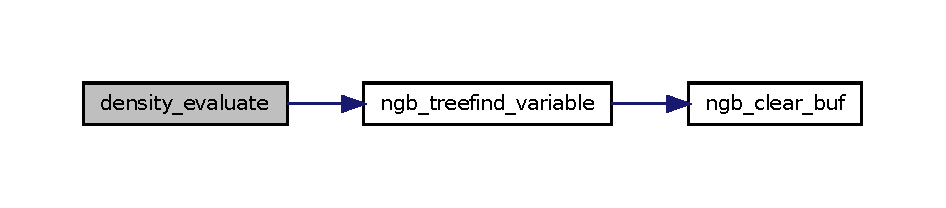
\includegraphics[width=350pt]{density_8c_a4e6b32342a24a33518b6ae8723809749_cgraph}
\end{center}
\end{figure}




\-Here is the caller graph for this function\-:
\nopagebreak
\begin{figure}[H]
\begin{center}
\leavevmode
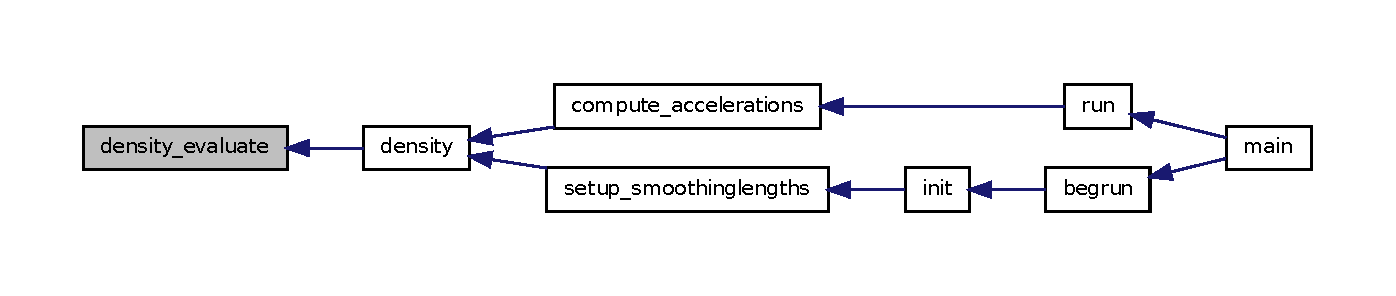
\includegraphics[width=350pt]{density_8c_a4e6b32342a24a33518b6ae8723809749_icgraph}
\end{center}
\end{figure}




\subsection{\-Variable \-Documentation}
\hypertarget{density_8c_af62571c97dc75a691aeafead0528b369}{\index{density.\-c@{density.\-c}!box\-Half@{box\-Half}}
\index{box\-Half@{box\-Half}!density.c@{density.\-c}}
\subsubsection[{box\-Half}]{\setlength{\rightskip}{0pt plus 5cm}double {\bf box\-Half}\hspace{0.3cm}{\ttfamily  \mbox{[}static\mbox{]}}}}\label{density_8c_af62571c97dc75a691aeafead0528b369}


\-Definition at line 22 of file density.\-c.



\-Referenced by density().

\hypertarget{density_8c_ac9067960018a06b81c117434c01f19cc}{\index{density.\-c@{density.\-c}!box\-Size@{box\-Size}}
\index{box\-Size@{box\-Size}!density.c@{density.\-c}}
\subsubsection[{box\-Size}]{\setlength{\rightskip}{0pt plus 5cm}double {\bf box\-Size}\hspace{0.3cm}{\ttfamily  \mbox{[}static\mbox{]}}}}\label{density_8c_ac9067960018a06b81c117434c01f19cc}


\-Definition at line 22 of file density.\-c.



\-Referenced by density(), and fill\-\_\-write\-\_\-buffer().


\hypertarget{domain_8c}{
\section{domain.c File Reference}
\label{domain_8c}\index{domain.c@{domain.c}}
}


code for domain decomposition  


{\ttfamily \#include $<$stdio.h$>$}\par
{\ttfamily \#include $<$stdlib.h$>$}\par
{\ttfamily \#include $<$string.h$>$}\par
{\ttfamily \#include $<$math.h$>$}\par
{\ttfamily \#include $<$mpi.h$>$}\par
{\ttfamily \#include \char`\"{}allvars.h\char`\"{}}\par
{\ttfamily \#include \char`\"{}proto.h\char`\"{}}\par
Include dependency graph for domain.c:\nopagebreak
\begin{figure}[H]
\begin{center}
\leavevmode
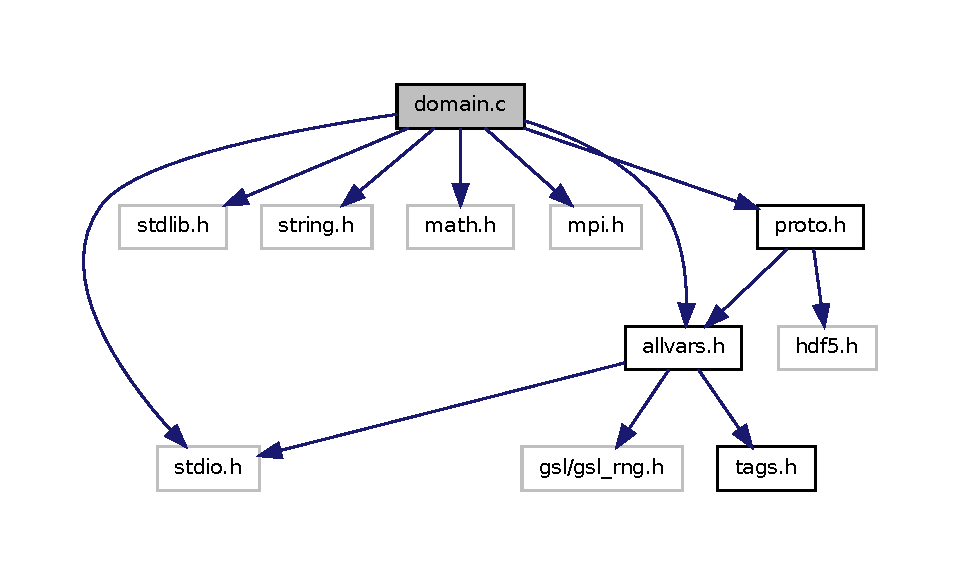
\includegraphics[width=400pt]{domain_8c__incl}
\end{center}
\end{figure}
\subsection*{Data Structures}
\begin{DoxyCompactItemize}
\item 
struct \hyperlink{structtopnode__exchange}{topnode\_\-exchange}
\end{DoxyCompactItemize}
\subsection*{Defines}
\begin{DoxyCompactItemize}
\item 
\#define \hyperlink{domain_8c_aebefeda80791480c21adcdd296f92c90}{TOPNODEFACTOR}~20.0
\item 
\#define \hyperlink{domain_8c_a503173887b0902500751aee72367e074}{REDUC\_\-FAC}~0.98
\end{DoxyCompactItemize}
\subsection*{Functions}
\begin{DoxyCompactItemize}
\item 
void \hyperlink{domain_8c_ae8e3aa408eaab9544cb7f93e69185492}{domain\_\-Decomposition} (void)
\item 
void \hyperlink{domain_8c_a647e0c1a76b7f064ed5d201662f364bf}{domain\_\-decompose} (void)
\item 
int \hyperlink{domain_8c_a412d5d8810751249cc8dcd9e219e4e57}{domain\_\-findSplit} (int cpustart, int ncpu, int first, int \hyperlink{forcetree_8c_a72e27dee31b1c4c6a504fbed29542d97}{last})
\item 
void \hyperlink{domain_8c_a89c54187117b91d4270a4f0c406ce2ba}{domain\_\-shiftSplit} (void)
\item 
void \hyperlink{domain_8c_a0e758ec7eef32fc7180092547f5a11b9}{domain\_\-findExchangeNumbers} (int task, int partner, int sphflag, int $\ast$send, int $\ast$recv)
\item 
void \hyperlink{domain_8c_ab7d41435f73c1626208d63b2d5ba28ca}{domain\_\-exchangeParticles} (int partner, int sphflag, int send\_\-count, int recv\_\-count)
\item 
void \hyperlink{domain_8c_a77c115c3aa2069d0eb8521329be0483c}{domain\_\-countToGo} (void)
\item 
void \hyperlink{domain_8c_a9b1062a5c460164de378d5e8c45736c4}{domain\_\-walktoptree} (int no)
\item 
void \hyperlink{domain_8c_a25aada0d3751c2afd2a376151d1d917e}{domain\_\-sumCost} (void)
\item 
void \hyperlink{domain_8c_add5620cbc133c73f0ce7da3a8fe9c01e}{domain\_\-findExtent} (void)
\item 
void \hyperlink{domain_8c_a25b4f5eb395f918bad4b4bc1fc3dc729}{domain\_\-determineTopTree} (void)
\item 
void \hyperlink{domain_8c_aa5001f9be833c4673392b40e7be3a421}{domain\_\-topsplit\_\-local} (int node, \hyperlink{allvars_8h_a63f10772bd5776dcb4b6301f425e0d26}{peanokey} startkey)
\item 
void \hyperlink{domain_8c_a606de536756a67ad8f79f1135009195e}{domain\_\-topsplit} (int node, \hyperlink{allvars_8h_a63f10772bd5776dcb4b6301f425e0d26}{peanokey} startkey)
\item 
int \hyperlink{domain_8c_a381621bc90438c5a50826bfdac8e4700}{domain\_\-compare\_\-toplist} (const void $\ast$a, const void $\ast$b)
\item 
int \hyperlink{domain_8c_a5b596de46669fab5e125f163d44edc37}{domain\_\-compare\_\-key} (const void $\ast$a, const void $\ast$b)
\end{DoxyCompactItemize}
\subsection*{Variables}
\begin{DoxyCompactItemize}
\item 
static int $\ast$ \hyperlink{domain_8c_a52aefc67245e1a334c311a420f89130c}{toGo}
\item 
static int $\ast$ \hyperlink{domain_8c_af00bb52ac4aa095d4d6daac54833675f}{toGoSph}
\item 
static int $\ast$ \hyperlink{domain_8c_a394783c89866b4e48255038384f9539b}{local\_\-toGo}
\item 
static int $\ast$ \hyperlink{domain_8c_a119a354c6c46ee11fdb9c7ad131b787a}{local\_\-toGoSph}
\item 
static int $\ast$ \hyperlink{domain_8c_a040694ce8b01a0b994df96d39588813a}{list\_\-NumPart}
\item 
static int $\ast$ \hyperlink{domain_8c_a9819cd512382caee762325ea86f4b221}{list\_\-N\_\-gas}
\item 
static int $\ast$ \hyperlink{domain_8c_af3343810478135e16ac72ea1f0172cd6}{list\_\-load}
\item 
static int $\ast$ \hyperlink{domain_8c_a97ae02d63ef3ac017dcbaea0d3b4dda4}{list\_\-loadsph}
\item 
static double $\ast$ \hyperlink{domain_8c_ad25e64ba07e1ed5350cceeab486c6f4a}{list\_\-work}
\item 
static long long \hyperlink{domain_8c_ac54707073f160b11ee4ba864066487c3}{maxload}
\item 
static long long \hyperlink{domain_8c_afa6a98969329aca0189182e060a2834e}{maxloadsph}
\item 
static struct \hyperlink{structtopnode__exchange}{topnode\_\-exchange} $\ast$ \hyperlink{domain_8c_aa4d05cc74afde41e1777c117c9103471}{toplist}
\item 
static struct \hyperlink{structtopnode__exchange}{topnode\_\-exchange} $\ast$ \hyperlink{domain_8c_a62244375ee3d9bdb3f7428a58de42085}{toplist\_\-local}
\end{DoxyCompactItemize}


\subsection{Detailed Description}
code for domain decomposition This file contains the code for the domain decomposition of the simulation volume. The domains are constructed from disjoint subsets of the leaves of a fiducial top-\/level tree that covers the full simulation volume. Domain boundaries hence run along tree-\/node divisions of a fiducial global BH tree. As a result of this method, the tree force are in principle strictly independent of the way the domains are cut. The domain decomposition can be carried out for an arbitrary number of CPUs. Individual domains are not cubical, but spatially coherent since the leaves are traversed in a Peano-\/Hilbert order and individual domains form segments along this order. This also ensures that each domain has a small surface to volume ratio, which minimizes communication. 

Definition in file \hyperlink{domain_8c_source}{domain.c}.



\subsection{Define Documentation}
\hypertarget{domain_8c_a503173887b0902500751aee72367e074}{
\index{domain.c@{domain.c}!REDUC\_\-FAC@{REDUC\_\-FAC}}
\index{REDUC\_\-FAC@{REDUC\_\-FAC}!domain.c@{domain.c}}
\subsubsection[{REDUC\_\-FAC}]{\setlength{\rightskip}{0pt plus 5cm}\#define REDUC\_\-FAC~0.98}}
\label{domain_8c_a503173887b0902500751aee72367e074}


Definition at line 31 of file domain.c.

\hypertarget{domain_8c_aebefeda80791480c21adcdd296f92c90}{
\index{domain.c@{domain.c}!TOPNODEFACTOR@{TOPNODEFACTOR}}
\index{TOPNODEFACTOR@{TOPNODEFACTOR}!domain.c@{domain.c}}
\subsubsection[{TOPNODEFACTOR}]{\setlength{\rightskip}{0pt plus 5cm}\#define TOPNODEFACTOR~20.0}}
\label{domain_8c_aebefeda80791480c21adcdd296f92c90}


Definition at line 29 of file domain.c.



Referenced by domain\_\-topsplit(), and domain\_\-topsplit\_\-local().



\subsection{Function Documentation}
\hypertarget{domain_8c_a5b596de46669fab5e125f163d44edc37}{
\index{domain.c@{domain.c}!domain\_\-compare\_\-key@{domain\_\-compare\_\-key}}
\index{domain\_\-compare\_\-key@{domain\_\-compare\_\-key}!domain.c@{domain.c}}
\subsubsection[{domain\_\-compare\_\-key}]{\setlength{\rightskip}{0pt plus 5cm}int domain\_\-compare\_\-key (
\begin{DoxyParamCaption}
\item[{const void $\ast$}]{ a, }
\item[{const void $\ast$}]{ b}
\end{DoxyParamCaption}
)}}
\label{domain_8c_a5b596de46669fab5e125f163d44edc37}
This is a comparison kernel used in a sort routine. 

Definition at line 1119 of file domain.c.



Referenced by domain\_\-determineTopTree().




\begin{DoxyCode}
{
  if(*(peanokey *) a < *(peanokey *) b)
    return -1;

  if(*(peanokey *) a > *(peanokey *) b)
    return +1;

  return 0;
}
\end{DoxyCode}




Here is the caller graph for this function:\nopagebreak
\begin{figure}[H]
\begin{center}
\leavevmode
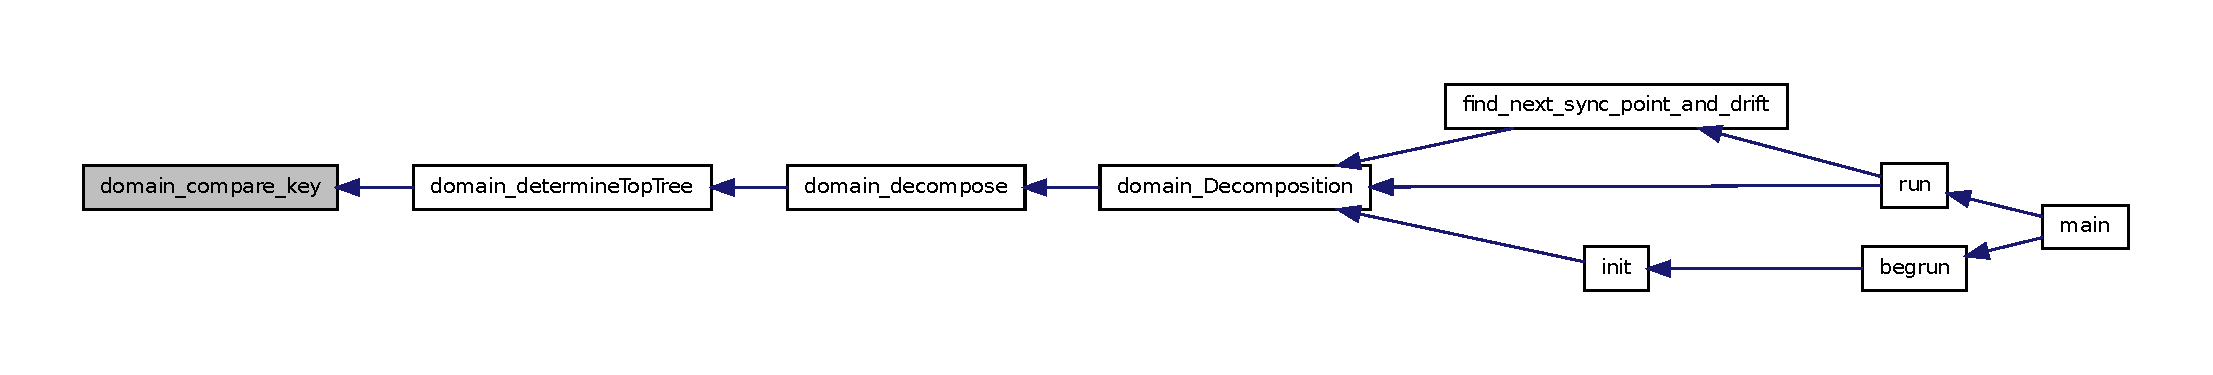
\includegraphics[width=400pt]{domain_8c_a5b596de46669fab5e125f163d44edc37_icgraph}
\end{center}
\end{figure}


\hypertarget{domain_8c_a381621bc90438c5a50826bfdac8e4700}{
\index{domain.c@{domain.c}!domain\_\-compare\_\-toplist@{domain\_\-compare\_\-toplist}}
\index{domain\_\-compare\_\-toplist@{domain\_\-compare\_\-toplist}!domain.c@{domain.c}}
\subsubsection[{domain\_\-compare\_\-toplist}]{\setlength{\rightskip}{0pt plus 5cm}int domain\_\-compare\_\-toplist (
\begin{DoxyParamCaption}
\item[{const void $\ast$}]{ a, }
\item[{const void $\ast$}]{ b}
\end{DoxyParamCaption}
)}}
\label{domain_8c_a381621bc90438c5a50826bfdac8e4700}
This is a comparison kernel used in a sort routine. 

Definition at line 1106 of file domain.c.



References topnode\_\-exchange::Startkey.



Referenced by domain\_\-determineTopTree().




\begin{DoxyCode}
{
  if(((struct topnode_exchange *) a)->Startkey < (((struct topnode_exchange *) b)
      ->Startkey))
    return -1;

  if(((struct topnode_exchange *) a)->Startkey > (((struct topnode_exchange *) b)
      ->Startkey))
    return +1;

  return 0;
}
\end{DoxyCode}




Here is the caller graph for this function:\nopagebreak
\begin{figure}[H]
\begin{center}
\leavevmode
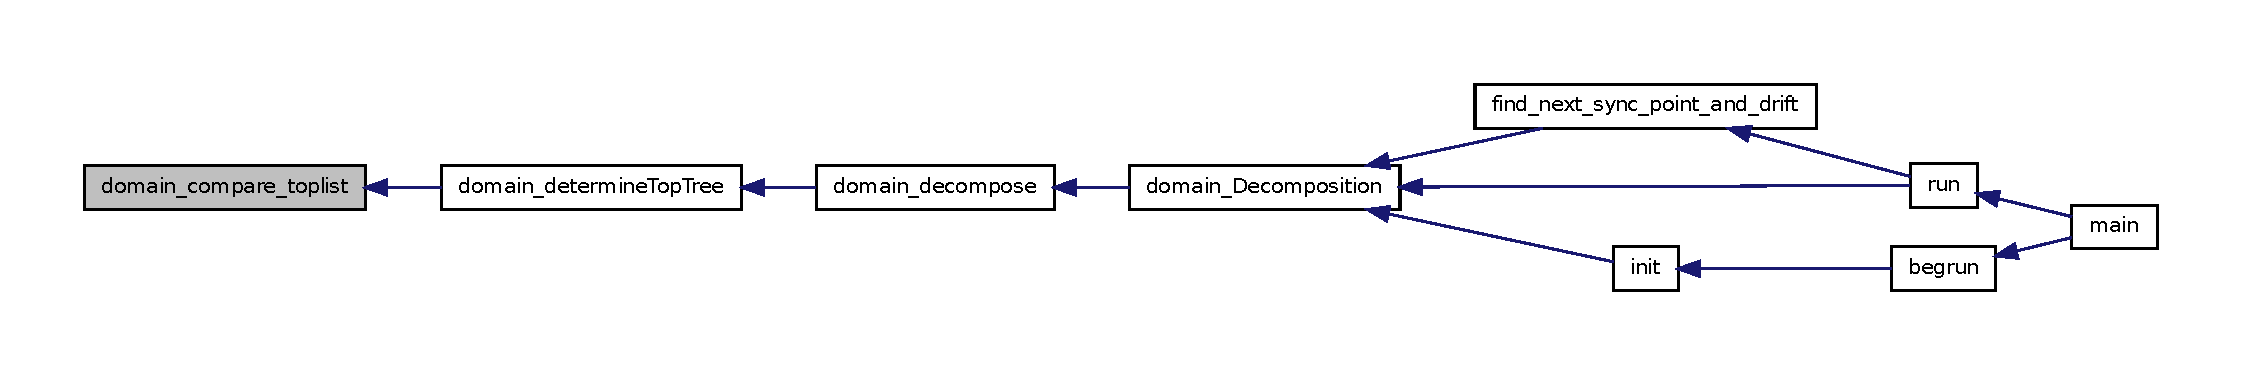
\includegraphics[width=400pt]{domain_8c_a381621bc90438c5a50826bfdac8e4700_icgraph}
\end{center}
\end{figure}


\hypertarget{domain_8c_a77c115c3aa2069d0eb8521329be0483c}{
\index{domain.c@{domain.c}!domain\_\-countToGo@{domain\_\-countToGo}}
\index{domain\_\-countToGo@{domain\_\-countToGo}!domain.c@{domain.c}}
\subsubsection[{domain\_\-countToGo}]{\setlength{\rightskip}{0pt plus 5cm}void domain\_\-countToGo (
\begin{DoxyParamCaption}
\item[{void}]{}
\end{DoxyParamCaption}
)}}
\label{domain_8c_a77c115c3aa2069d0eb8521329be0483c}
This function determines how many particles that are currently stored on the local CPU have to be moved off according to the domain decomposition. 

Definition at line 729 of file domain.c.



References topnode\_\-data::Daughter, DomainTask, Key, topnode\_\-data::Leaf, local\_\-toGo, local\_\-toGoSph, NTask, NumPart, P, topnode\_\-data::StartKey, ThisTask, toGo, toGoSph, and TopNodes.



Referenced by domain\_\-decompose().




\begin{DoxyCode}
{
  int n, no;

  for(n = 0; n < NTask; n++)
    {
      local_toGo[n] = 0;
      local_toGoSph[n] = 0;
    }

  for(n = 0; n < NumPart; n++)
    {
      no = 0;

      while(TopNodes[no].Daughter >= 0)
        no = TopNodes[no].Daughter + (Key[n] - TopNodes[no].StartKey) / (
      TopNodes[no].Size / 8);

      no = TopNodes[no].Leaf;

      if(DomainTask[no] != ThisTask)
        {
          local_toGo[DomainTask[no]] += 1;
          if(P[n].Type == 0)
            local_toGoSph[DomainTask[no]] += 1;
        }
    }

  MPI_Allgather(local_toGo, NTask, MPI_INT, toGo, NTask, MPI_INT, MPI_COMM_WORLD)
      ;
  MPI_Allgather(local_toGoSph, NTask, MPI_INT, toGoSph, NTask, MPI_INT, MPI_COMM_
      WORLD);
}
\end{DoxyCode}




Here is the caller graph for this function:\nopagebreak
\begin{figure}[H]
\begin{center}
\leavevmode
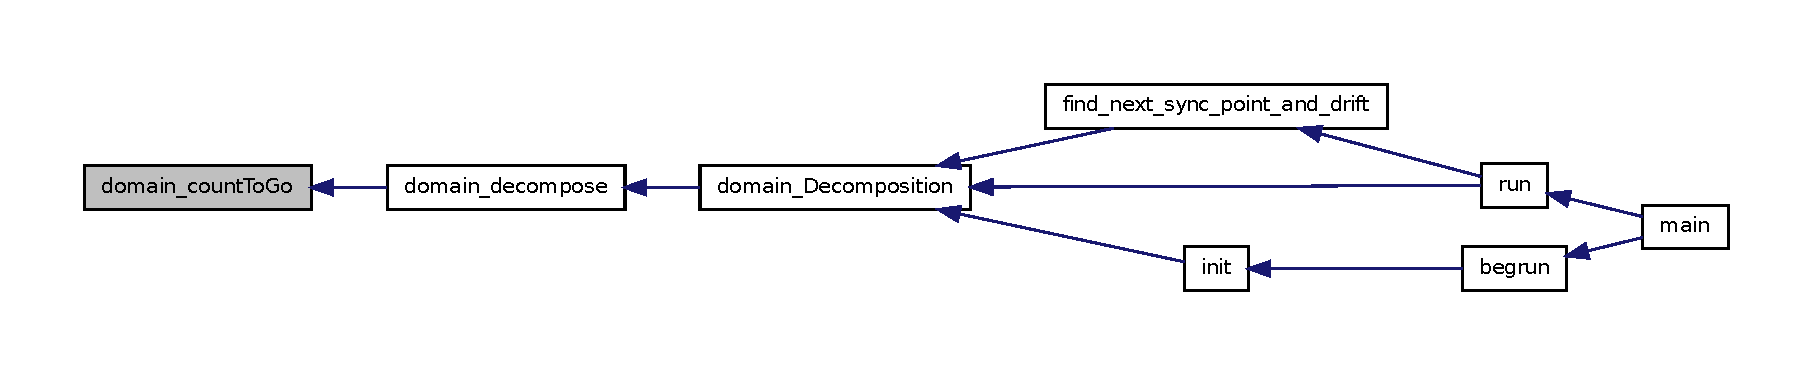
\includegraphics[width=400pt]{domain_8c_a77c115c3aa2069d0eb8521329be0483c_icgraph}
\end{center}
\end{figure}


\hypertarget{domain_8c_a647e0c1a76b7f064ed5d201662f364bf}{
\index{domain.c@{domain.c}!domain\_\-decompose@{domain\_\-decompose}}
\index{domain\_\-decompose@{domain\_\-decompose}!domain.c@{domain.c}}
\subsubsection[{domain\_\-decompose}]{\setlength{\rightskip}{0pt plus 5cm}void domain\_\-decompose (
\begin{DoxyParamCaption}
\item[{void}]{}
\end{DoxyParamCaption}
)}}
\label{domain_8c_a647e0c1a76b7f064ed5d201662f364bf}
This function carries out the actual domain decomposition for all particle types. It will try to balance the work-\/load for each domain, as estimated based on the P\mbox{[}i\mbox{]}-\/GravCost values. The decomposition will respect the maximum allowed memory-\/imbalance given by the value of PartAllocFactor. 

Definition at line 154 of file domain.c.



References All, domain\_\-countToGo(), domain\_\-determineTopTree(), domain\_\-exchangeParticles(), domain\_\-findExchangeNumbers(), domain\_\-findExtent(), domain\_\-findSplit(), domain\_\-shiftSplit(), domain\_\-sumCost(), DomainEndList, DomainMyLast, DomainMyStart, DomainStartList, endrun(), list\_\-load, list\_\-N\_\-gas, list\_\-NumPart, list\_\-work, maxload, NTask, NTopleaves, Ntype, NtypeLocal, NumPart, P, PTask, global\_\-data\_\-all\_\-processes::SofteningTable, ThisTask, toGo, toGoSph, and global\_\-data\_\-all\_\-processes::TotN\_\-gas.



Referenced by domain\_\-Decomposition().




\begin{DoxyCode}
{
  int i, j, status;
  int ngrp, task, partner, sendcount, recvcount;
  long long sumtogo, sumload;
  int maxload, *temp;
  double sumwork, maxwork;

  for(i = 0; i < 6; i++)
    NtypeLocal[i] = 0;

  for(i = 0; i < NumPart; i++)
    NtypeLocal[P[i].Type]++;

  /* because Ntype[] is of type `long long', we cannot do a simple
   * MPI_Allreduce() to sum the total particle numbers 
   */
  temp = malloc(NTask * 6 * sizeof(int));
  MPI_Allgather(NtypeLocal, 6, MPI_INT, temp, 6, MPI_INT, MPI_COMM_WORLD);
  for(i = 0; i < 6; i++)
    {
      Ntype[i] = 0;
      for(j = 0; j < NTask; j++)
        Ntype[i] += temp[j * 6 + i];
    }
  free(temp);

#ifndef UNEQUALSOFTENINGS
  for(i = 0; i < 6; i++)
    if(Ntype[i] > 0)
      break;

  for(ngrp = i + 1; ngrp < 6; ngrp++)
    {
      if(Ntype[ngrp] > 0)
        if(All.SofteningTable[ngrp] != All.SofteningTable[i])
          {
            if(ThisTask == 0)
              {
                fprintf(stdout, "Code was not compiled with UNEQUALSOFTENINGS, bu
      t some of the\n");
                fprintf(stdout, "softening lengths are unequal nevertheless.\n");
      
                fprintf(stdout, "This is not allowed.\n");
              }
            endrun(0);
          }
    }
#endif


  /* determine global dimensions of domain grid */
  domain_findExtent();

  domain_determineTopTree();

  /* determine cost distribution in domain grid */
  domain_sumCost();

  /* find the split of the domain grid recursively */
  status = domain_findSplit(0, NTask, 0, NTopleaves - 1);
  if(status != 0)
    {
      if(ThisTask == 0)
        printf("\nNo domain decomposition that stays within memory bounds is poss
      ible.\n");
      endrun(0);
    }

  /* now try to improve the work-load balance of the split */
  domain_shiftSplit();

  DomainMyStart = DomainStartList[ThisTask];
  DomainMyLast = DomainEndList[ThisTask];

  if(ThisTask == 0)
    {
      sumload = maxload = 0;
      sumwork = maxwork = 0;
      for(i = 0; i < NTask; i++)
        {
          sumload += list_load[i];
          sumwork += list_work[i];

          if(list_load[i] > maxload)
            maxload = list_load[i];

          if(list_work[i] > maxwork)
            maxwork = list_work[i];
        }

      printf("work-load balance=%g   memory-balance=%g\n",
             maxwork / (sumwork / NTask), maxload / (((double) sumload) / NTask))
      ;
    }


  /* determine for each cpu how many particles have to be shifted to other cpus *
      /
  domain_countToGo();

  for(i = 0, sumtogo = 0; i < NTask * NTask; i++)
    sumtogo += toGo[i];

  while(sumtogo > 0)
    {
      if(ThisTask == 0)
        {
          printf("exchange of %d%09d particles\n", (int) (sumtogo / 1000000000),
                 (int) (sumtogo % 1000000000));
          fflush(stdout);
        }

      for(ngrp = 1; ngrp < (1 << PTask); ngrp++)
        {
          for(task = 0; task < NTask; task++)
            {
              partner = task ^ ngrp;

              if(partner < NTask && task < partner)
                {
                  /* treat SPH separately */
                  if(All.TotN_gas > 0)
                    {
                      domain_findExchangeNumbers(task, partner, 1, &sendcount, &r
      ecvcount);

                      list_NumPart[task] += recvcount - sendcount;
                      list_NumPart[partner] -= recvcount - sendcount;
                      list_N_gas[task] += recvcount - sendcount;
                      list_N_gas[partner] -= recvcount - sendcount;

                      toGo[task * NTask + partner] -= sendcount;
                      toGo[partner * NTask + task] -= recvcount;
                      toGoSph[task * NTask + partner] -= sendcount;
                      toGoSph[partner * NTask + task] -= recvcount;

                      if(task == ThisTask)      /* actually carry out the exchang
      e */
                        domain_exchangeParticles(partner, 1, sendcount, recvcount
      );
                      if(partner == ThisTask)
                        domain_exchangeParticles(task, 1, recvcount, sendcount);
                    }

                  domain_findExchangeNumbers(task, partner, 0, &sendcount, &recvc
      ount);

                  list_NumPart[task] += recvcount - sendcount;
                  list_NumPart[partner] -= recvcount - sendcount;

                  toGo[task * NTask + partner] -= sendcount;
                  toGo[partner * NTask + task] -= recvcount;

                  if(task == ThisTask)  /* actually carry out the exchange */
                    domain_exchangeParticles(partner, 0, sendcount, recvcount);
                  if(partner == ThisTask)
                    domain_exchangeParticles(task, 0, recvcount, sendcount);
                }
            }
        }

      for(i = 0, sumtogo = 0; i < NTask * NTask; i++)
        sumtogo += toGo[i];
    }
}
\end{DoxyCode}




Here is the call graph for this function:\nopagebreak
\begin{figure}[H]
\begin{center}
\leavevmode
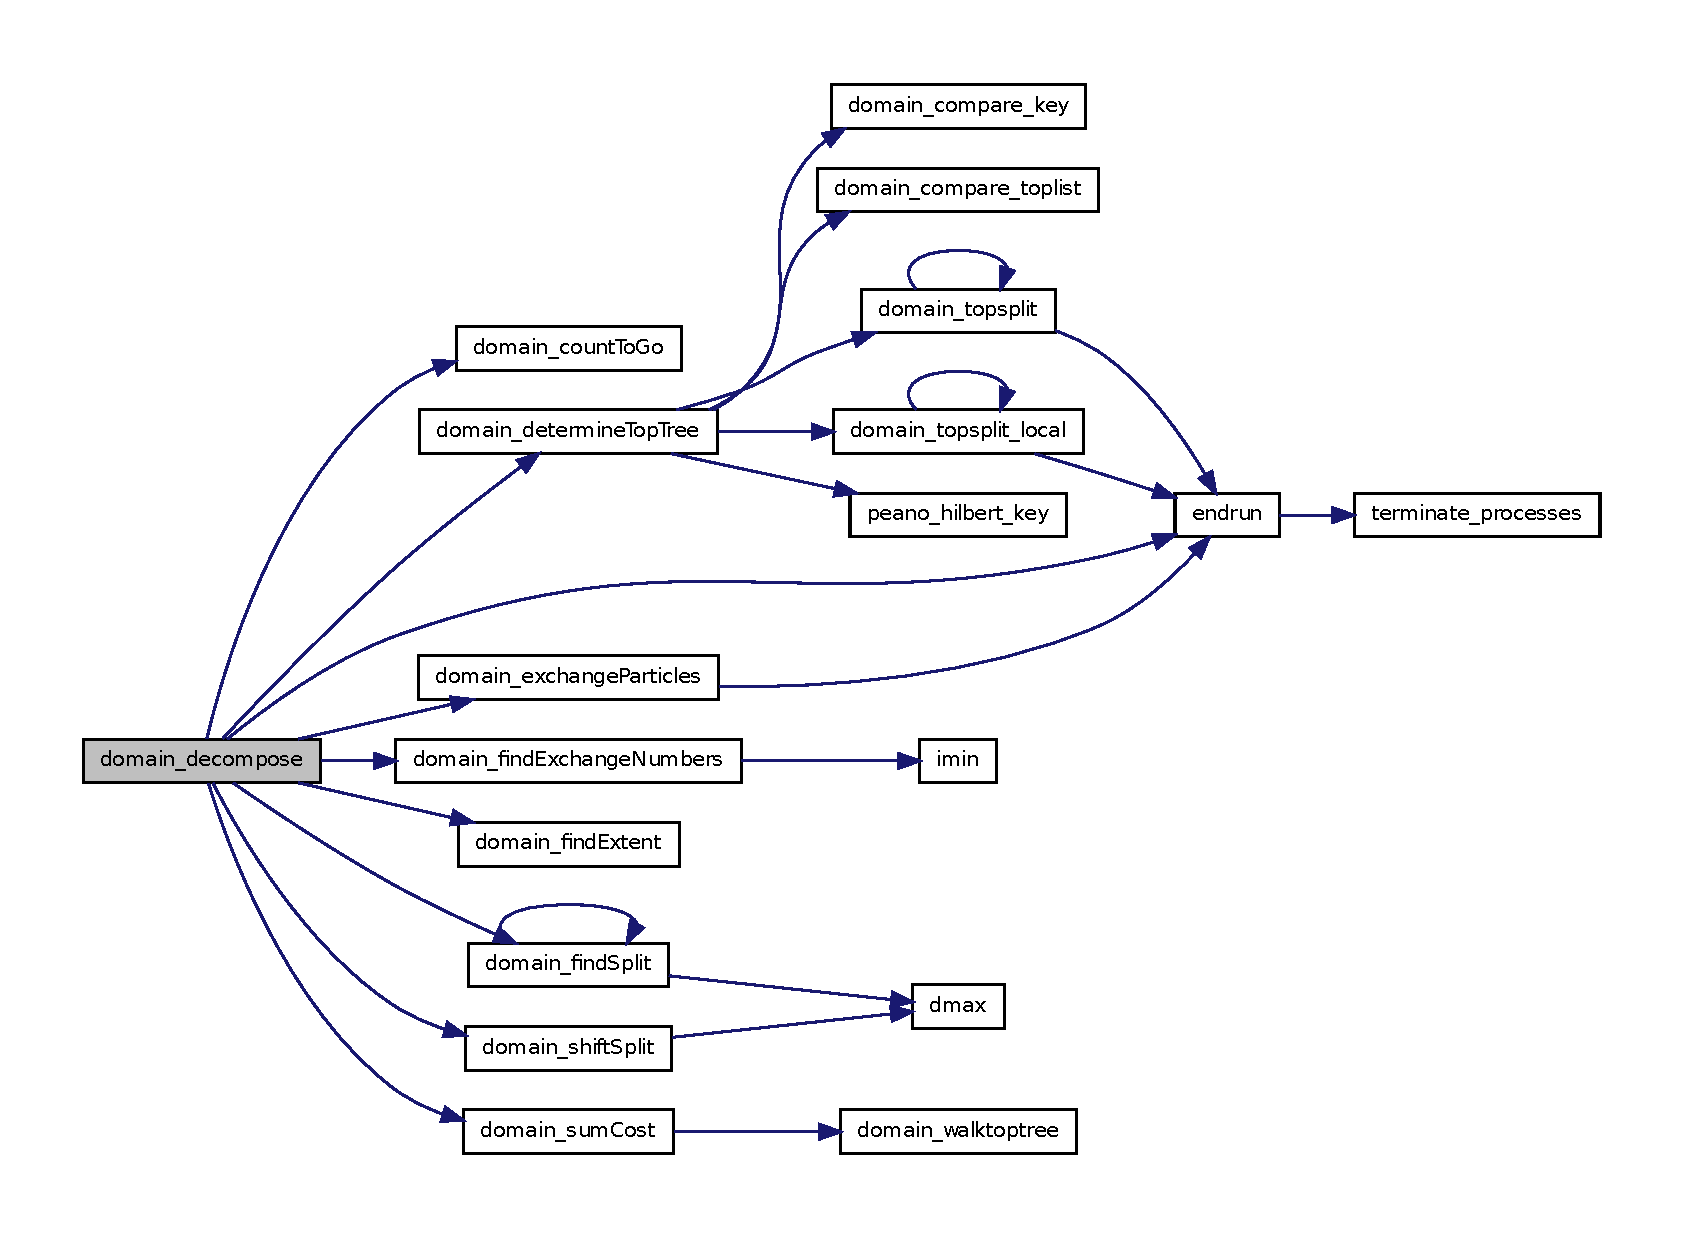
\includegraphics[width=400pt]{domain_8c_a647e0c1a76b7f064ed5d201662f364bf_cgraph}
\end{center}
\end{figure}




Here is the caller graph for this function:\nopagebreak
\begin{figure}[H]
\begin{center}
\leavevmode
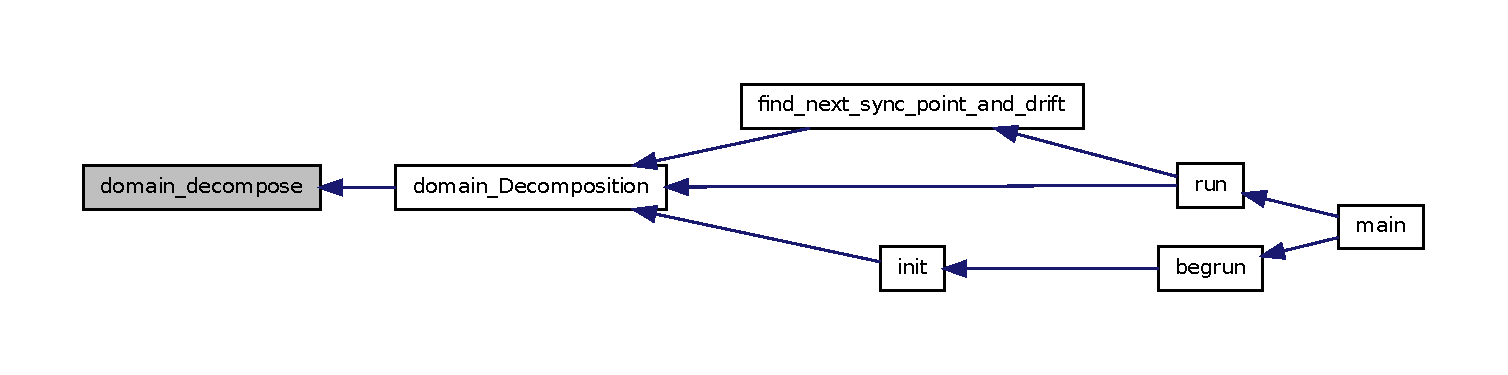
\includegraphics[width=400pt]{domain_8c_a647e0c1a76b7f064ed5d201662f364bf_icgraph}
\end{center}
\end{figure}


\hypertarget{domain_8c_ae8e3aa408eaab9544cb7f93e69185492}{
\index{domain.c@{domain.c}!domain\_\-Decomposition@{domain\_\-Decomposition}}
\index{domain\_\-Decomposition@{domain\_\-Decomposition}!domain.c@{domain.c}}
\subsubsection[{domain\_\-Decomposition}]{\setlength{\rightskip}{0pt plus 5cm}void domain\_\-Decomposition (
\begin{DoxyParamCaption}
\item[{void}]{}
\end{DoxyParamCaption}
)}}
\label{domain_8c_ae8e3aa408eaab9544cb7f93e69185492}
This is the main routine for the domain decomposition. It acts as a driver routine that allocates various temporary buffers, maps the particles back onto the periodic box if needed, and then does the domain decomposition, and a final Peano-\/Hilbert order of all particles as a tuning measure. 

Definition at line 62 of file domain.c.



References All, global\_\-data\_\-all\_\-processes::CPU\_\-Domain, global\_\-data\_\-all\_\-processes::CPU\_\-Peano, do\_\-box\_\-wrapping(), domain\_\-decompose(), Key, KeySorted, list\_\-load, list\_\-loadsph, list\_\-N\_\-gas, list\_\-NumPart, list\_\-work, local\_\-toGo, local\_\-toGoSph, maxload, maxloadsph, global\_\-data\_\-all\_\-processes::MaxPart, global\_\-data\_\-all\_\-processes::MaxPartSph, N\_\-gas, NTask, global\_\-data\_\-all\_\-processes::NumForcesSinceLastDomainDecomp, NumPart, peano\_\-hilbert\_\-order(), global\_\-data\_\-all\_\-processes::PM\_\-Ti\_\-endstep, second(), ThisTask, global\_\-data\_\-all\_\-processes::Ti\_\-Current, timediff(), toGo, toGoSph, global\_\-data\_\-all\_\-processes::TotNumPart, global\_\-data\_\-all\_\-processes::TreeDomainUpdateFrequency, and TreeReconstructFlag.



Referenced by find\_\-next\_\-sync\_\-point\_\-and\_\-drift(), init(), and run().




\begin{DoxyCode}
{
  double t0, t1;

#ifdef PMGRID
  if(All.PM_Ti_endstep == All.Ti_Current)
    {
      All.NumForcesSinceLastDomainDecomp = 1 + All.TotNumPart * All.
      TreeDomainUpdateFrequency;
      /* to make sure that we do a domain decomposition before the PM-force is ev
      aluated.
         this is needed to make sure that the particles are wrapped into the box 
      */
    }
#endif

  /* Check whether it is really time for a new domain decomposition */
  if(All.NumForcesSinceLastDomainDecomp > All.TotNumPart * All.
      TreeDomainUpdateFrequency)
    {
      t0 = second();

#ifdef PERIODIC
      do_box_wrapping();        /* map the particles back onto the box */
#endif
      All.NumForcesSinceLastDomainDecomp = 0;
      TreeReconstructFlag = 1;  /* ensures that new tree will be constructed */

      if(ThisTask == 0)
        {
          printf("domain decomposition... \n");
          fflush(stdout);
        }

      Key = malloc(sizeof(peanokey) * All.MaxPart);
      KeySorted = malloc(sizeof(peanokey) * All.MaxPart);

      toGo = malloc(sizeof(int) * NTask * NTask);
      toGoSph = malloc(sizeof(int) * NTask * NTask);
      local_toGo = malloc(sizeof(int) * NTask);
      local_toGoSph = malloc(sizeof(int) * NTask);
      list_NumPart = malloc(sizeof(int) * NTask);
      list_N_gas = malloc(sizeof(int) * NTask);
      list_load = malloc(sizeof(int) * NTask);
      list_loadsph = malloc(sizeof(int) * NTask);
      list_work = malloc(sizeof(double) * NTask);

      MPI_Allgather(&NumPart, 1, MPI_INT, list_NumPart, 1, MPI_INT, MPI_COMM_WORL
      D);
      MPI_Allgather(&N_gas, 1, MPI_INT, list_N_gas, 1, MPI_INT, MPI_COMM_WORLD);

      maxload = All.MaxPart * REDUC_FAC;
      maxloadsph = All.MaxPartSph * REDUC_FAC;

      domain_decompose();

      free(list_work);
      free(list_loadsph);
      free(list_load);
      free(list_N_gas);
      free(list_NumPart);
      free(local_toGoSph);
      free(local_toGo);
      free(toGoSph);
      free(toGo);


      if(ThisTask == 0)
        {
          printf("domain decomposition done. \n");
          fflush(stdout);
        }

      t1 = second();
      All.CPU_Domain += timediff(t0, t1);

#ifdef PEANOHILBERT
      t0 = second();
      peano_hilbert_order();
      t1 = second();
      All.CPU_Peano += timediff(t0, t1);
#endif

      free(KeySorted);
      free(Key);
    }

}
\end{DoxyCode}




Here is the call graph for this function:\nopagebreak
\begin{figure}[H]
\begin{center}
\leavevmode
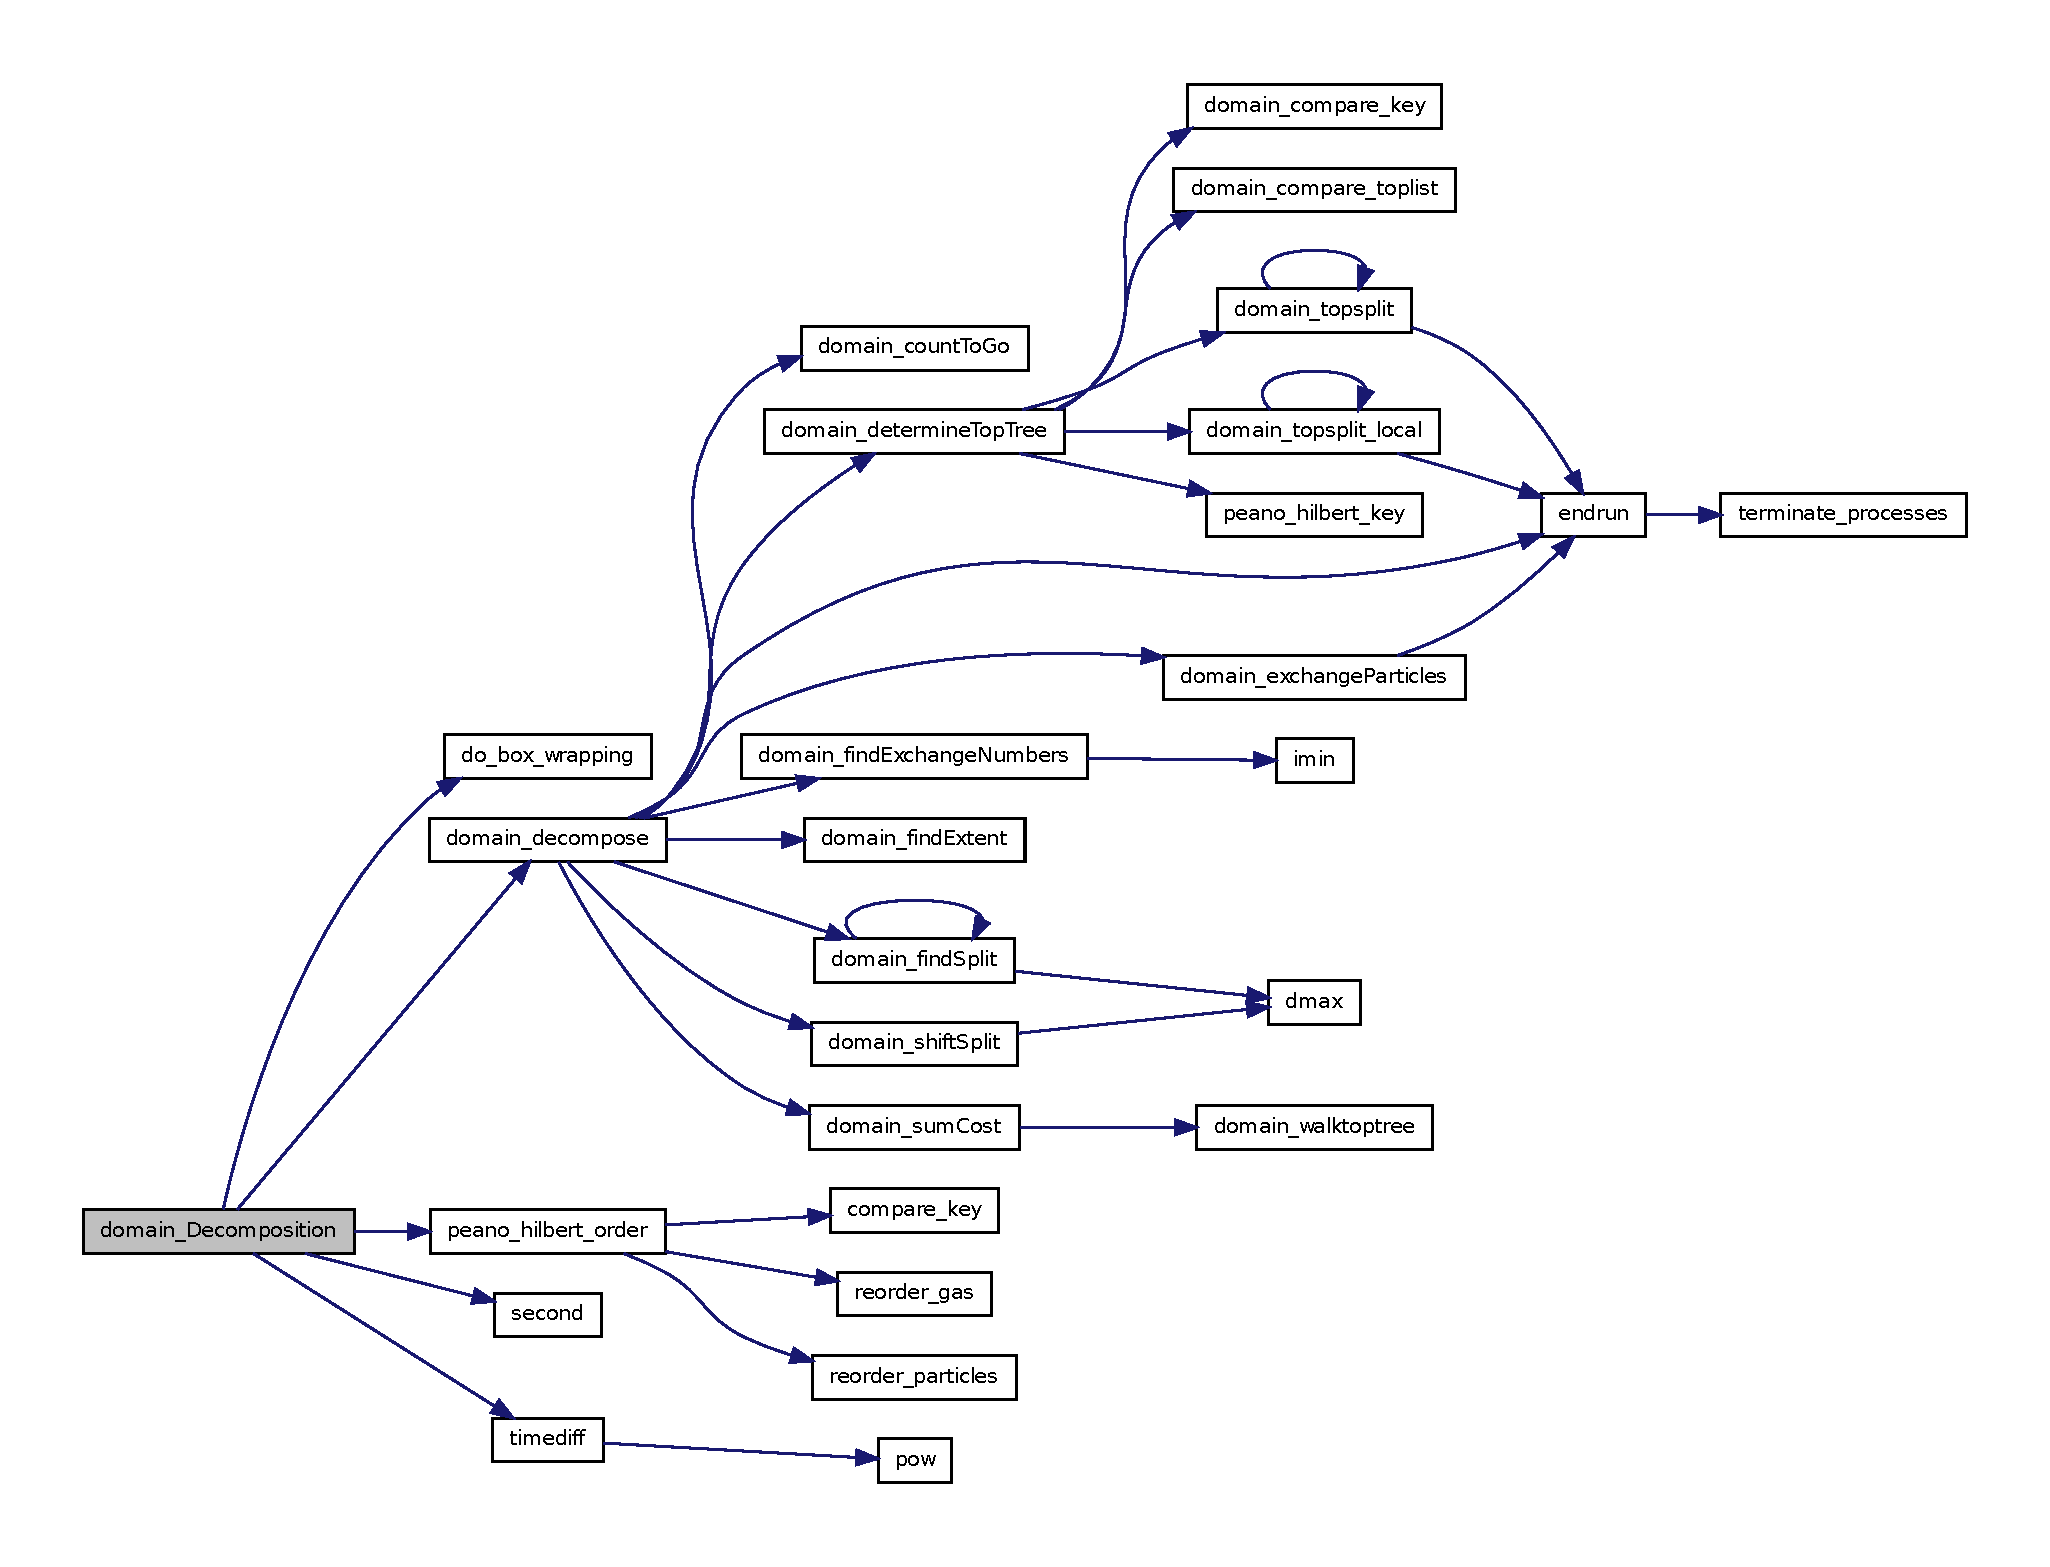
\includegraphics[width=400pt]{domain_8c_ae8e3aa408eaab9544cb7f93e69185492_cgraph}
\end{center}
\end{figure}




Here is the caller graph for this function:\nopagebreak
\begin{figure}[H]
\begin{center}
\leavevmode
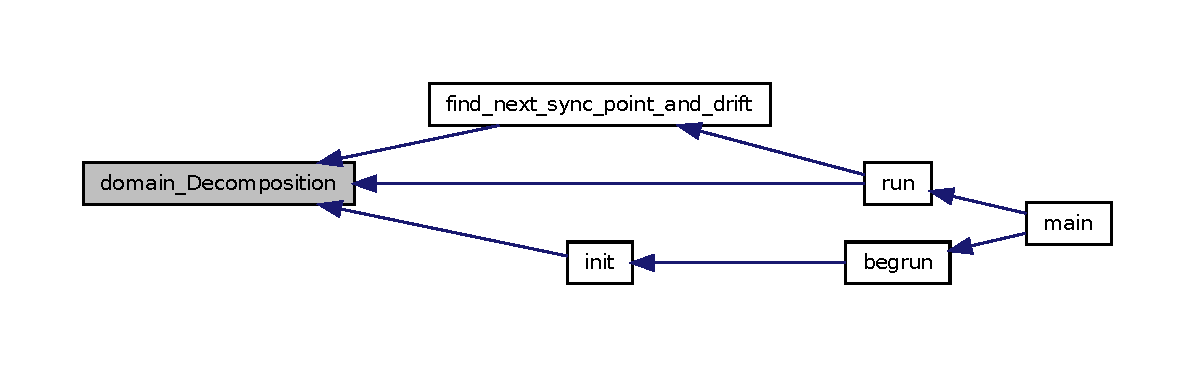
\includegraphics[width=400pt]{domain_8c_ae8e3aa408eaab9544cb7f93e69185492_icgraph}
\end{center}
\end{figure}


\hypertarget{domain_8c_a25b4f5eb395f918bad4b4bc1fc3dc729}{
\index{domain.c@{domain.c}!domain\_\-determineTopTree@{domain\_\-determineTopTree}}
\index{domain\_\-determineTopTree@{domain\_\-determineTopTree}!domain.c@{domain.c}}
\subsubsection[{domain\_\-determineTopTree}]{\setlength{\rightskip}{0pt plus 5cm}void domain\_\-determineTopTree (
\begin{DoxyParamCaption}
\item[{void}]{}
\end{DoxyParamCaption}
)}}
\label{domain_8c_a25b4f5eb395f918bad4b4bc1fc3dc729}
This function constructs the global top-\/level tree node that is used for the domain decomposition. This is done by considering the string of Peano-\/Hilbert keys for all particles, which is recursively chopped off in pieces of eight segments until each segment holds at most a certain number of particles. 

$<$ Bits per dimension available for Peano-\/Hilbert order. Note: If peanokey is defined 0 0 int, the allowed maximum is 10. If 64-\/bit integers are used, the maximum is 21

$<$ Bits per dimension available for Peano-\/Hilbert order. Note: If peanokey is defined 0 0 0 , the allowed maximum is 10. If 64-\/bit integers are used, the maximum is 21

$<$ The number of different Peano-\/Hilbert cells

$<$ Bits per dimension available for Peano-\/Hilbert order. Note: If peanokey is defined 0 0 0 , the allowed maximum is 10. If 64-\/bit integers are used, the maximum is 21

$<$ The number of different Peano-\/Hilbert cells 



Definition at line 896 of file domain.c.



References All, BITS\_\-PER\_\-DIMENSION, topnode\_\-data::Blocks, topnode\_\-exchange::Count, topnode\_\-data::Count, topnode\_\-data::Daughter, domain\_\-compare\_\-key(), domain\_\-compare\_\-toplist(), domain\_\-topsplit(), domain\_\-topsplit\_\-local(), DomainCorner, DomainFac, Key, KeySorted, NTask, NTopnodes, NumPart, P, peano\_\-hilbert\_\-key(), topnode\_\-data::Pstart, topnode\_\-data::Size, topnode\_\-exchange::Startkey, topnode\_\-data::StartKey, toplist, toplist\_\-local, TopNodes, and global\_\-data\_\-all\_\-processes::TotNumPart.



Referenced by domain\_\-decompose().




\begin{DoxyCode}
{
  int i, ntop_local, ntop;
  int *ntopnodelist, *ntopoffset;

  for(i = 0; i < NumPart; i++)
    {
      KeySorted[i] = Key[i] = peano_hilbert_key((P[i].Pos[0] - DomainCorner[0]) *
       DomainFac,
                                                (P[i].Pos[1] - DomainCorner[1]) *
       DomainFac,
                                                (P[i].Pos[2] - DomainCorner[2]) *
       DomainFac,
                                                BITS_PER_DIMENSION);
    }

  qsort(KeySorted, NumPart, sizeof(peanokey), domain_compare_key);

  NTopnodes = 1;
  TopNodes[0].Daughter = -1;
  TopNodes[0].Size = PEANOCELLS;
  TopNodes[0].StartKey = 0;
  TopNodes[0].Count = NumPart;
  TopNodes[0].Pstart = 0;

  domain_topsplit_local(0, 0);

  toplist_local = malloc(NTopnodes * sizeof(struct topnode_exchange));

  for(i = 0, ntop_local = 0; i < NTopnodes; i++)
    {
      if(TopNodes[i].Daughter == -1)    /* only use leaves */
        {
          toplist_local[ntop_local].Startkey = TopNodes[i].StartKey;
          toplist_local[ntop_local].Count = TopNodes[i].Count;
          ntop_local++;
        }
    }

  ntopnodelist = malloc(sizeof(int) * NTask);
  ntopoffset = malloc(sizeof(int) * NTask);

  MPI_Allgather(&ntop_local, 1, MPI_INT, ntopnodelist, 1, MPI_INT, MPI_COMM_WORLD
      );

  for(i = 0, ntop = 0, ntopoffset[0] = 0; i < NTask; i++)
    {
      ntop += ntopnodelist[i];
      if(i > 0)
        ntopoffset[i] = ntopoffset[i - 1] + ntopnodelist[i - 1];
    }


  toplist = malloc(ntop * sizeof(struct topnode_exchange));

  for(i = 0; i < NTask; i++)
    {
      ntopnodelist[i] *= sizeof(struct topnode_exchange);
      ntopoffset[i] *= sizeof(struct topnode_exchange);
    }

  MPI_Allgatherv(toplist_local, ntop_local * sizeof(struct topnode_exchange), MPI
      _BYTE,
                 toplist, ntopnodelist, ntopoffset, MPI_BYTE, MPI_COMM_WORLD);

  qsort(toplist, ntop, sizeof(struct topnode_exchange), domain_compare_toplist);

  NTopnodes = 1;
  TopNodes[0].Daughter = -1;
  TopNodes[0].Size = PEANOCELLS;
  TopNodes[0].StartKey = 0;
  TopNodes[0].Count = All.TotNumPart;
  TopNodes[0].Pstart = 0;
  TopNodes[0].Blocks = ntop;

  domain_topsplit(0, 0);

  free(toplist);
  free(ntopoffset);
  free(ntopnodelist);
  free(toplist_local);

}
\end{DoxyCode}




Here is the call graph for this function:\nopagebreak
\begin{figure}[H]
\begin{center}
\leavevmode
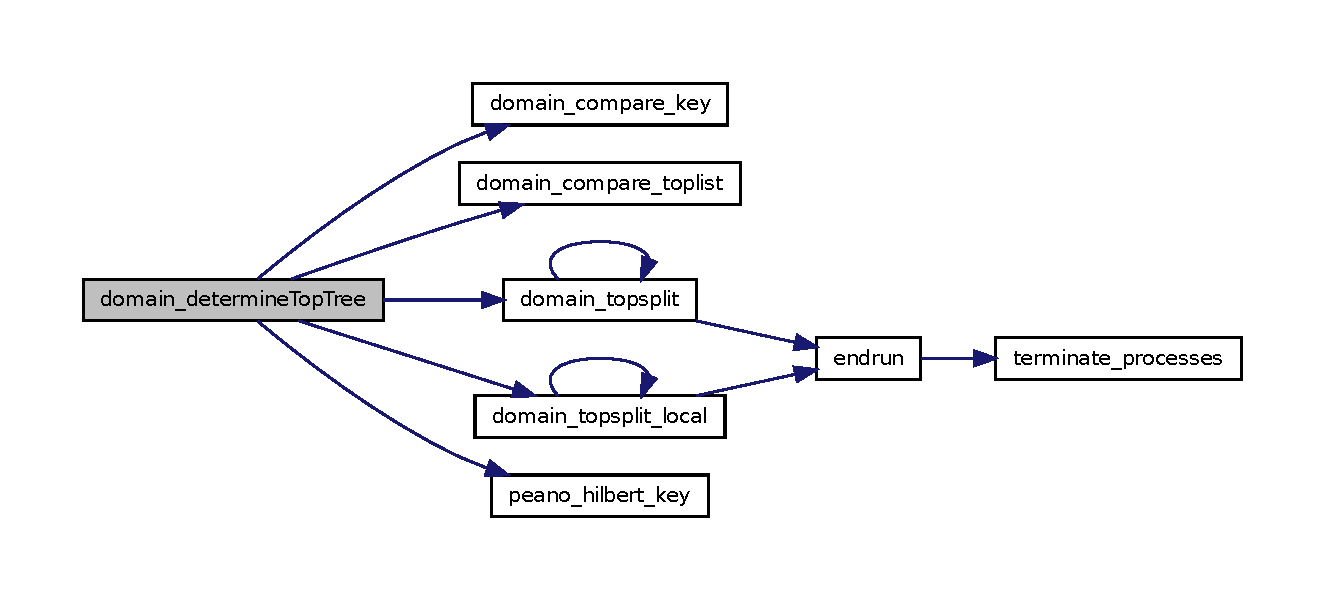
\includegraphics[width=400pt]{domain_8c_a25b4f5eb395f918bad4b4bc1fc3dc729_cgraph}
\end{center}
\end{figure}




Here is the caller graph for this function:\nopagebreak
\begin{figure}[H]
\begin{center}
\leavevmode
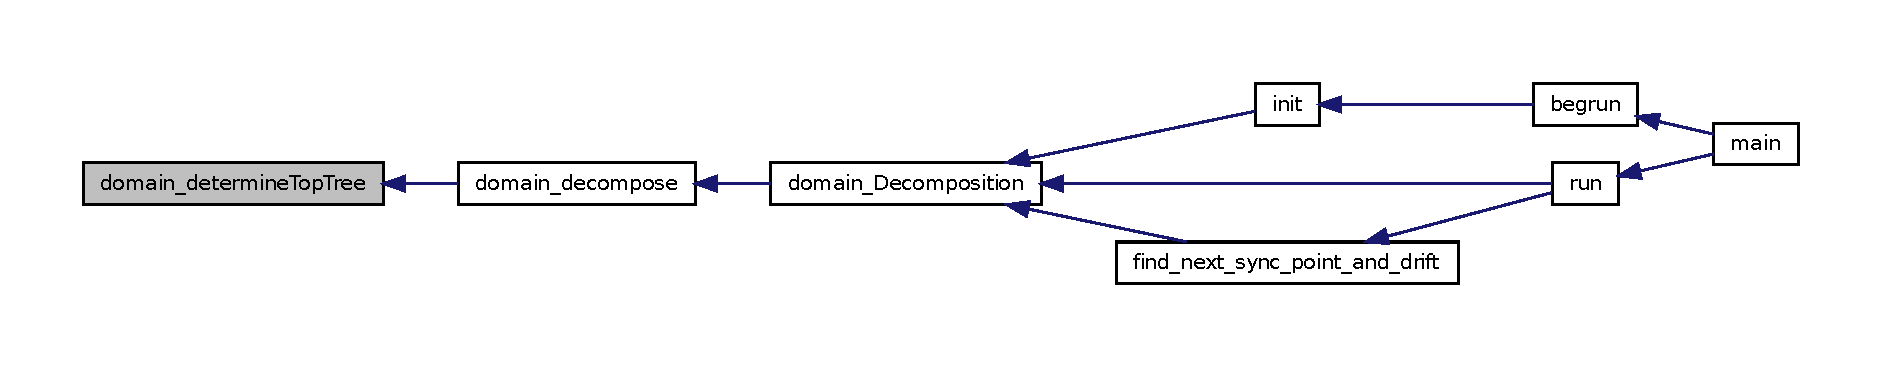
\includegraphics[width=400pt]{domain_8c_a25b4f5eb395f918bad4b4bc1fc3dc729_icgraph}
\end{center}
\end{figure}


\hypertarget{domain_8c_ab7d41435f73c1626208d63b2d5ba28ca}{
\index{domain.c@{domain.c}!domain\_\-exchangeParticles@{domain\_\-exchangeParticles}}
\index{domain\_\-exchangeParticles@{domain\_\-exchangeParticles}!domain.c@{domain.c}}
\subsubsection[{domain\_\-exchangeParticles}]{\setlength{\rightskip}{0pt plus 5cm}void domain\_\-exchangeParticles (
\begin{DoxyParamCaption}
\item[{int}]{ partner, }
\item[{int}]{ sphflag, }
\item[{int}]{ send\_\-count, }
\item[{int}]{ recv\_\-count}
\end{DoxyParamCaption}
)}}
\label{domain_8c_ab7d41435f73c1626208d63b2d5ba28ca}
This function exchanges particles between two CPUs according to the domain split. In doing this, the memory boundaries which may restrict the exhange process are observed. 

Definition at line 595 of file domain.c.



References topnode\_\-data::Daughter, DomainKeyBuf, DomainPartBuf, DomainSphBuf, DomainTask, endrun(), Key, topnode\_\-data::Leaf, N\_\-gas, NumPart, P, SphP, topnode\_\-data::StartKey, TAG\_\-KEY, TAG\_\-PDATA, TAG\_\-SPHDATA, ThisTask, and TopNodes.



Referenced by domain\_\-decompose().




\begin{DoxyCode}
{
  int i, no, n, count, rep;
  MPI_Status status;

  for(n = 0, count = 0; count < send_count && n < NumPart; n++)
    {
      if(sphflag)
        {
          if(P[n].Type != 0)
            continue;
        }
      else
        {
          if(P[n].Type == 0)
            continue;
        }

      no = 0;

      while(TopNodes[no].Daughter >= 0)
        no = TopNodes[no].Daughter + (Key[n] - TopNodes[no].StartKey) / (
      TopNodes[no].Size / 8);

      no = TopNodes[no].Leaf;

      if(DomainTask[no] == partner)
        {
          if(sphflag)           /* special reorder routine for SPH particles (nee
      d to stay at beginning) */
            {
              DomainPartBuf[count] = P[n];      /* copy particle and collect in c
      ontiguous memory */
              DomainKeyBuf[count] = Key[n];
              DomainSphBuf[count] = SphP[n];

              P[n] = P[N_gas - 1];
              P[N_gas - 1] = P[NumPart - 1];

              Key[n] = Key[N_gas - 1];
              Key[N_gas - 1] = Key[NumPart - 1];

              SphP[n] = SphP[N_gas - 1];

              N_gas--;
            }
          else
            {
              DomainPartBuf[count] = P[n];      /* copy particle and collect in c
      ontiguous memory */
              DomainKeyBuf[count] = Key[n];
              P[n] = P[NumPart - 1];
              Key[n] = Key[NumPart - 1];
            }

          count++;
          NumPart--;
          n--;
        }
    }

  if(count != send_count)
    {
      printf("Houston, we got a problem...\n");
      printf("ThisTask=%d count=%d send_count=%d\n", ThisTask, count, send_count)
      ;
      endrun(88);
    }

  /* transmit */

  for(rep = 0; rep < 2; rep++)
    {
      if((rep == 0 && ThisTask < partner) || (rep == 1 && ThisTask > partner))
        {
          if(send_count > 0)
            {
              MPI_Ssend(&DomainPartBuf[0], send_count * sizeof(struct 
      particle_data), MPI_BYTE, partner,
                        TAG_PDATA, MPI_COMM_WORLD);

              MPI_Ssend(&DomainKeyBuf[0], send_count * sizeof(peanokey), MPI_BYTE
      , partner, TAG_KEY,
                        MPI_COMM_WORLD);

              if(sphflag)
                MPI_Ssend(&DomainSphBuf[0], send_count * sizeof(struct 
      sph_particle_data), MPI_BYTE, partner,
                          TAG_SPHDATA, MPI_COMM_WORLD);
            }
        }

      if((rep == 1 && ThisTask < partner) || (rep == 0 && ThisTask > partner))
        {
          if(recv_count > 0)
            {
              if(sphflag)
                {
                  if((NumPart - N_gas) > recv_count)
                    {
                      for(i = 0; i < recv_count; i++)
                        {
                          P[NumPart + i] = P[N_gas + i];
                          Key[NumPart + i] = Key[N_gas + i];
                        }
                    }
                  else
                    {
                      for(i = NumPart - 1; i >= N_gas; i--)
                        {
                          P[i + recv_count] = P[i];
                          Key[i + recv_count] = Key[i];
                        }
                    }

                  MPI_Recv(&P[N_gas], recv_count * sizeof(struct particle_data), 
      MPI_BYTE, partner, TAG_PDATA,
                           MPI_COMM_WORLD, &status);
                  MPI_Recv(&Key[N_gas], recv_count * sizeof(peanokey), MPI_BYTE, 
      partner, TAG_KEY,
                           MPI_COMM_WORLD, &status);
                  MPI_Recv(&SphP[N_gas], recv_count * sizeof(struct 
      sph_particle_data), MPI_BYTE, partner,
                           TAG_SPHDATA, MPI_COMM_WORLD, &status);

                  N_gas += recv_count;
                }
              else
                {
                  MPI_Recv(&P[NumPart], recv_count * sizeof(struct particle_data)
      , MPI_BYTE, partner,
                           TAG_PDATA, MPI_COMM_WORLD, &status);
                  MPI_Recv(&Key[NumPart], recv_count * sizeof(peanokey), MPI_BYTE
      , partner,
                           TAG_KEY, MPI_COMM_WORLD, &status);
                }

              NumPart += recv_count;
            }
        }
    }
}
\end{DoxyCode}




Here is the call graph for this function:\nopagebreak
\begin{figure}[H]
\begin{center}
\leavevmode
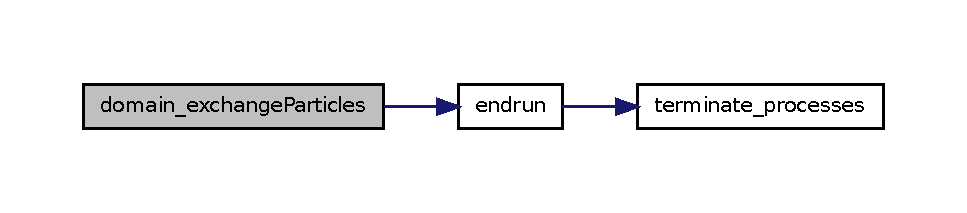
\includegraphics[width=400pt]{domain_8c_ab7d41435f73c1626208d63b2d5ba28ca_cgraph}
\end{center}
\end{figure}




Here is the caller graph for this function:\nopagebreak
\begin{figure}[H]
\begin{center}
\leavevmode
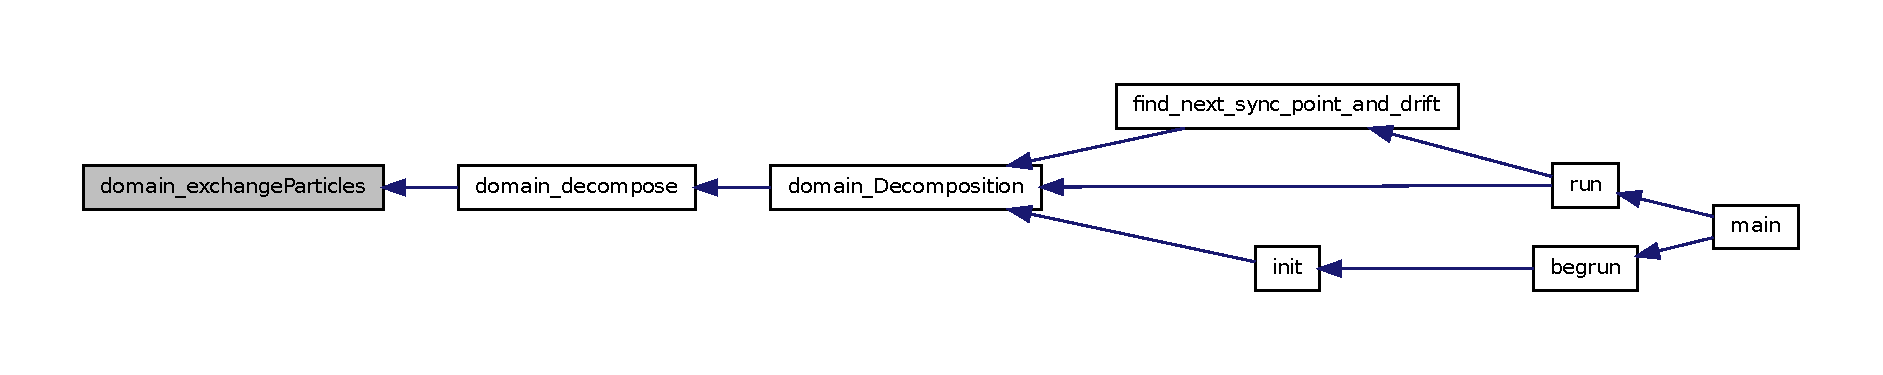
\includegraphics[width=400pt]{domain_8c_ab7d41435f73c1626208d63b2d5ba28ca_icgraph}
\end{center}
\end{figure}


\hypertarget{domain_8c_a0e758ec7eef32fc7180092547f5a11b9}{
\index{domain.c@{domain.c}!domain\_\-findExchangeNumbers@{domain\_\-findExchangeNumbers}}
\index{domain\_\-findExchangeNumbers@{domain\_\-findExchangeNumbers}!domain.c@{domain.c}}
\subsubsection[{domain\_\-findExchangeNumbers}]{\setlength{\rightskip}{0pt plus 5cm}void domain\_\-findExchangeNumbers (
\begin{DoxyParamCaption}
\item[{int}]{ task, }
\item[{int}]{ partner, }
\item[{int}]{ sphflag, }
\item[{int $\ast$}]{ send, }
\item[{int $\ast$}]{ recv}
\end{DoxyParamCaption}
)}}
\label{domain_8c_a0e758ec7eef32fc7180092547f5a11b9}
This function counts how many particles have to be exchanged between two CPUs according to the domain split. If the CPUs are already quite full and hold data from other CPUs as well, not all the particles may be exchanged at once. In this case the communication phase has to be repeated, until enough of the third-\/party particles have been moved away such that the decomposition can be completed. 

Definition at line 534 of file domain.c.



References All, global\_\-data\_\-all\_\-processes::BunchSizeDomain, imin(), list\_\-N\_\-gas, list\_\-NumPart, global\_\-data\_\-all\_\-processes::MaxPart, global\_\-data\_\-all\_\-processes::MaxPartSph, NTask, toGo, and toGoSph.



Referenced by domain\_\-decompose().




\begin{DoxyCode}
{
  int numpartA, numpartsphA, ntobesentA, maxsendA, maxsendA_old;
  int numpartB, numpartsphB, ntobesentB, maxsendB, maxsendB_old;

  numpartA = list_NumPart[task];
  numpartsphA = list_N_gas[task];

  numpartB = list_NumPart[partner];
  numpartsphB = list_N_gas[partner];

  if(sphflag == 1)
    {
      ntobesentA = toGoSph[task * NTask + partner];
      ntobesentB = toGoSph[partner * NTask + task];
    }
  else
    {
      ntobesentA = toGo[task * NTask + partner] - toGoSph[task * NTask + partner]
      ;
      ntobesentB = toGo[partner * NTask + task] - toGoSph[partner * NTask + task]
      ;
    }

  maxsendA = imin(ntobesentA, All.BunchSizeDomain);
  maxsendB = imin(ntobesentB, All.BunchSizeDomain);

  do
    {
      maxsendA_old = maxsendA;
      maxsendB_old = maxsendB;

      maxsendA = imin(All.MaxPart - numpartB + maxsendB, maxsendA);
      maxsendB = imin(All.MaxPart - numpartA + maxsendA, maxsendB);
    }
  while((maxsendA != maxsendA_old) || (maxsendB != maxsendB_old));


  /* now make also sure that there is enough space for SPH particeles */
  if(sphflag == 1)
    {
      do
        {
          maxsendA_old = maxsendA;
          maxsendB_old = maxsendB;

          maxsendA = imin(All.MaxPartSph - numpartsphB + maxsendB, maxsendA);
          maxsendB = imin(All.MaxPartSph - numpartsphA + maxsendA, maxsendB);
        }
      while((maxsendA != maxsendA_old) || (maxsendB != maxsendB_old));
    }

  *send = maxsendA;
  *recv = maxsendB;
}
\end{DoxyCode}




Here is the call graph for this function:\nopagebreak
\begin{figure}[H]
\begin{center}
\leavevmode
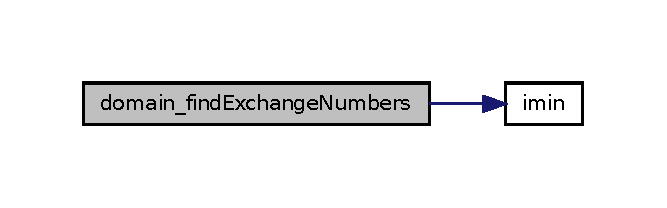
\includegraphics[width=320pt]{domain_8c_a0e758ec7eef32fc7180092547f5a11b9_cgraph}
\end{center}
\end{figure}




Here is the caller graph for this function:\nopagebreak
\begin{figure}[H]
\begin{center}
\leavevmode
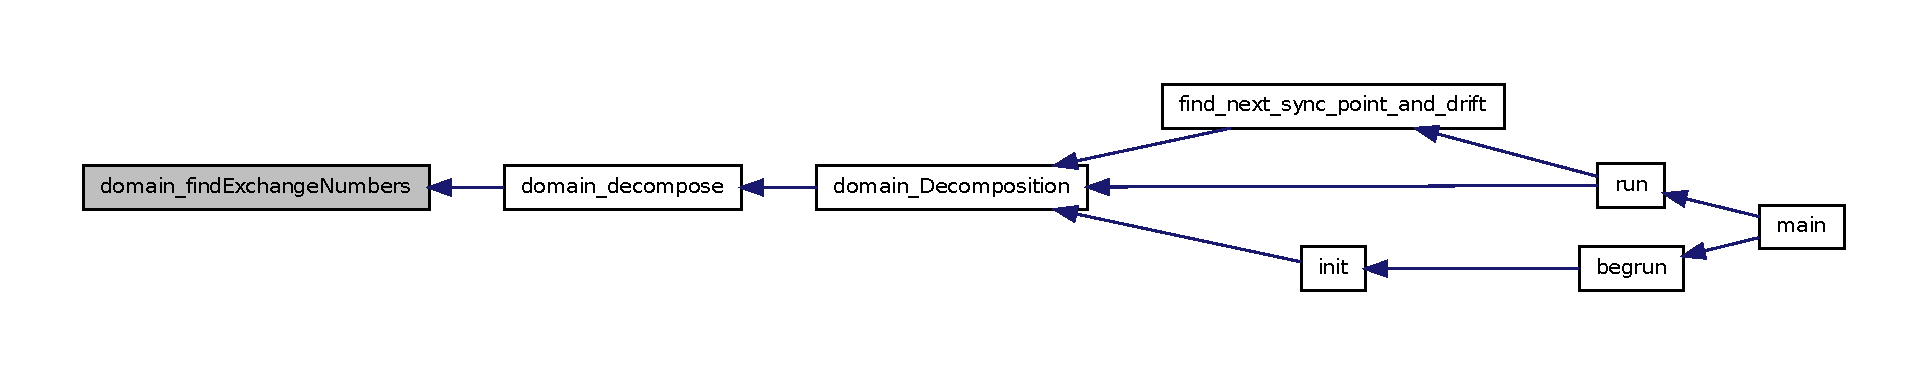
\includegraphics[width=400pt]{domain_8c_a0e758ec7eef32fc7180092547f5a11b9_icgraph}
\end{center}
\end{figure}


\hypertarget{domain_8c_add5620cbc133c73f0ce7da3a8fe9c01e}{
\index{domain.c@{domain.c}!domain\_\-findExtent@{domain\_\-findExtent}}
\index{domain\_\-findExtent@{domain\_\-findExtent}!domain.c@{domain.c}}
\subsubsection[{domain\_\-findExtent}]{\setlength{\rightskip}{0pt plus 5cm}void domain\_\-findExtent (
\begin{DoxyParamCaption}
\item[{void}]{}
\end{DoxyParamCaption}
)}}
\label{domain_8c_add5620cbc133c73f0ce7da3a8fe9c01e}
This routine finds the extent of the global domain grid. 

$<$ Bits per dimension available for Peano-\/Hilbert order. Note: If peanokey is defined 0 0 int, the allowed maximum is 10. If 64-\/bit integers are used, the maximum is 21 



Definition at line 845 of file domain.c.



References DomainCenter, DomainCorner, DomainFac, DomainLen, NumPart, P, and particle\_\-data::Pos.



Referenced by domain\_\-decompose().




\begin{DoxyCode}
{
  int i, j;
  double len, xmin[3], xmax[3], xmin_glob[3], xmax_glob[3];

  /* determine local extension */
  for(j = 0; j < 3; j++)
    {
      xmin[j] = MAX_REAL_NUMBER;
      xmax[j] = -MAX_REAL_NUMBER;
    }

  for(i = 0; i < NumPart; i++)
    {
      for(j = 0; j < 3; j++)
        {
          if(xmin[j] > P[i].Pos[j])
            xmin[j] = P[i].Pos[j];

          if(xmax[j] < P[i].Pos[j])
            xmax[j] = P[i].Pos[j];
        }
    }

  MPI_Allreduce(xmin, xmin_glob, 3, MPI_DOUBLE, MPI_MIN, MPI_COMM_WORLD);
  MPI_Allreduce(xmax, xmax_glob, 3, MPI_DOUBLE, MPI_MAX, MPI_COMM_WORLD);

  len = 0;
  for(j = 0; j < 3; j++)
    if(xmax_glob[j] - xmin_glob[j] > len)
      len = xmax_glob[j] - xmin_glob[j];

  len *= 1.001;

  for(j = 0; j < 3; j++)
    {
      DomainCenter[j] = 0.5 * (xmin_glob[j] + xmax_glob[j]);
      DomainCorner[j] = 0.5 * (xmin_glob[j] + xmax_glob[j]) - 0.5 * len;
    }

  DomainLen = len;
  DomainFac = 1.0 / len * (((peanokey) 1) << (BITS_PER_DIMENSION));
}
\end{DoxyCode}




Here is the caller graph for this function:\nopagebreak
\begin{figure}[H]
\begin{center}
\leavevmode
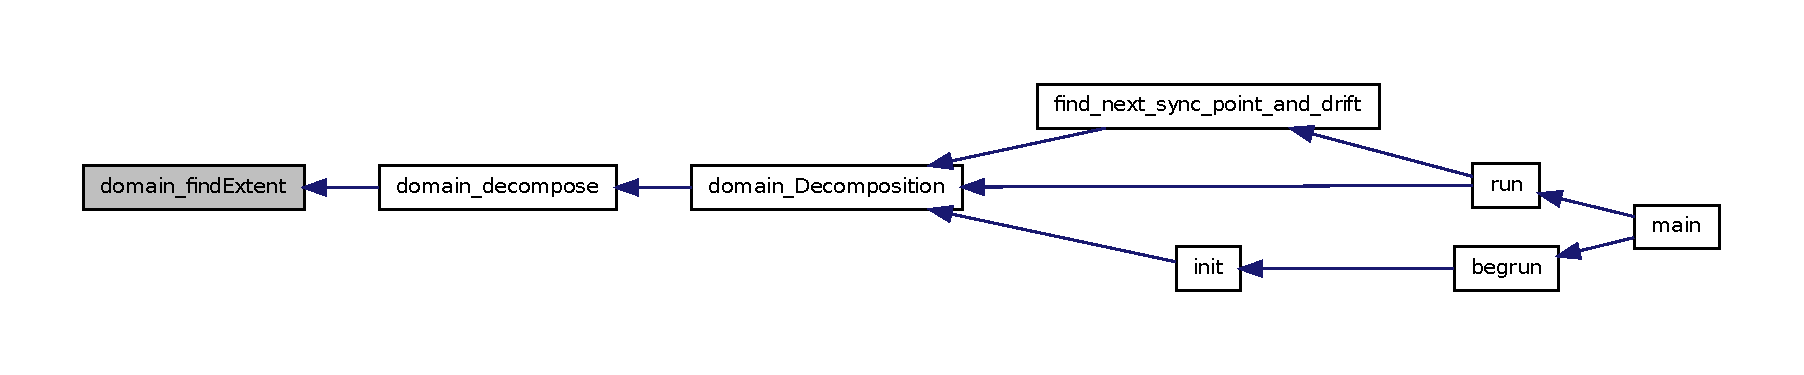
\includegraphics[width=400pt]{domain_8c_add5620cbc133c73f0ce7da3a8fe9c01e_icgraph}
\end{center}
\end{figure}


\hypertarget{domain_8c_a412d5d8810751249cc8dcd9e219e4e57}{
\index{domain.c@{domain.c}!domain\_\-findSplit@{domain\_\-findSplit}}
\index{domain\_\-findSplit@{domain\_\-findSplit}!domain.c@{domain.c}}
\subsubsection[{domain\_\-findSplit}]{\setlength{\rightskip}{0pt plus 5cm}int domain\_\-findSplit (
\begin{DoxyParamCaption}
\item[{int}]{ cpustart, }
\item[{int}]{ ncpu, }
\item[{int}]{ first, }
\item[{int}]{ last}
\end{DoxyParamCaption}
)}}
\label{domain_8c_a412d5d8810751249cc8dcd9e219e4e57}
This function tries to find a split point in a range of cells in the domain-\/grid. The range of cells starts at 'first', and ends at 'last' (inclusively). The number of cpus that holds the range is 'ncpu', with the first cpu given by 'cpustart'. If more than 2 cpus are to be split, the function calls itself recursively. The division tries to achieve a best particle-\/load balance under the constraint that 'maxload' and 'maxloadsph' may not be exceeded, and that each cpu holds at least one cell from the domaingrid. If such a decomposition cannot be achieved, a non-\/zero error code is returned.

After successful completion, DomainMyStart\mbox{[}\mbox{]} and DomainMyLast\mbox{[}\mbox{]} contain the first and last cell of the domaingrid assigned to the local task for the given type. Also, DomainTask\mbox{[}\mbox{]} contains for each cell the task it was assigned to. 

Definition at line 327 of file domain.c.



References dmax(), domain\_\-findSplit(), DomainCount, DomainCountSph, DomainEndList, DomainStartList, DomainTask, list\_\-load, list\_\-loadsph, maxload, and maxloadsph.



Referenced by domain\_\-decompose(), and domain\_\-findSplit().




\begin{DoxyCode}
{
  int i, split, ok_left, ok_right;
  long long load, sphload, load_leftOfSplit, sphload_leftOfSplit;
  int ncpu_leftOfSplit;
  double maxAvgLoad_CurrentSplit, maxAvgLoad_NewSplit;


  ncpu_leftOfSplit = ncpu / 2;

  for(i = first, load = 0, sphload = 0; i <= last; i++)
    {
      load += DomainCount[i];
      sphload += DomainCountSph[i];
    }

  split = first + ncpu_leftOfSplit;

  for(i = first, load_leftOfSplit = sphload_leftOfSplit = 0; i < split; i++)
    {
      load_leftOfSplit += DomainCount[i];
      sphload_leftOfSplit += DomainCountSph[i];
    }

  /* find the best split point in terms of work-load balance */

  while(split < last - (ncpu - ncpu_leftOfSplit - 1) && split > 0)
    {
      maxAvgLoad_CurrentSplit =
        dmax(load_leftOfSplit / ncpu_leftOfSplit, (load - load_leftOfSplit) / (nc
      pu - ncpu_leftOfSplit));

      maxAvgLoad_NewSplit =
        dmax((load_leftOfSplit + DomainCount[split]) / ncpu_leftOfSplit,
             (load - load_leftOfSplit - DomainCount[split]) / (ncpu - ncpu_leftOf
      Split));

      if(maxAvgLoad_NewSplit <= maxAvgLoad_CurrentSplit)
        {
          load_leftOfSplit += DomainCount[split];
          sphload_leftOfSplit += DomainCountSph[split];
          split++;
        }
      else
        break;
    }


  /* we will now have to check whether this solution is possible given the restri
      ctions on the maximum load */

  for(i = first, load_leftOfSplit = 0, sphload_leftOfSplit = 0; i < split; i++)
    {
      load_leftOfSplit += DomainCount[i];
      sphload_leftOfSplit += DomainCountSph[i];
    }

  if(load_leftOfSplit > maxload * ncpu_leftOfSplit ||
     (load - load_leftOfSplit) > maxload * (ncpu - ncpu_leftOfSplit))
    {
      /* we did not find a viable split */
      return -1;
    }

  if(sphload_leftOfSplit > maxloadsph * ncpu_leftOfSplit ||
     (sphload - sphload_leftOfSplit) > maxloadsph * (ncpu - ncpu_leftOfSplit))
    {
      /* we did not find a viable split */
      return -1;
    }

  if(ncpu_leftOfSplit >= 2)
    ok_left = domain_findSplit(cpustart, ncpu_leftOfSplit, first, split - 1);
  else
    ok_left = 0;

  if((ncpu - ncpu_leftOfSplit) >= 2)
    ok_right = domain_findSplit(cpustart + ncpu_leftOfSplit, ncpu - ncpu_leftOfSp
      lit, split, last);
  else
    ok_right = 0;

  if(ok_left == 0 && ok_right == 0)
    {
      /* found a viable split */

      if(ncpu_leftOfSplit == 1)
        {
          for(i = first; i < split; i++)
            DomainTask[i] = cpustart;

          list_load[cpustart] = load_leftOfSplit;
          list_loadsph[cpustart] = sphload_leftOfSplit;
          DomainStartList[cpustart] = first;
          DomainEndList[cpustart] = split - 1;
        }

      if((ncpu - ncpu_leftOfSplit) == 1)
        {
          for(i = split; i <= last; i++)
            DomainTask[i] = cpustart + ncpu_leftOfSplit;

          list_load[cpustart + ncpu_leftOfSplit] = load - load_leftOfSplit;
          list_loadsph[cpustart + ncpu_leftOfSplit] = sphload - sphload_leftOfSpl
      it;
          DomainStartList[cpustart + ncpu_leftOfSplit] = split;
          DomainEndList[cpustart + ncpu_leftOfSplit] = last;
        }

      return 0;
    }

  /* we did not find a viable split */
  return -1;
}
\end{DoxyCode}




Here is the call graph for this function:\nopagebreak
\begin{figure}[H]
\begin{center}
\leavevmode
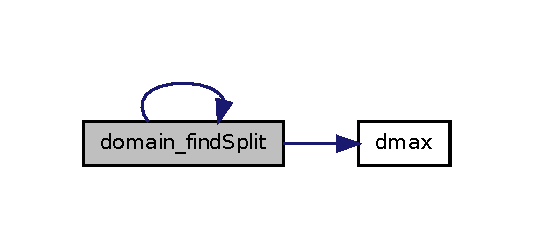
\includegraphics[width=256pt]{domain_8c_a412d5d8810751249cc8dcd9e219e4e57_cgraph}
\end{center}
\end{figure}




Here is the caller graph for this function:\nopagebreak
\begin{figure}[H]
\begin{center}
\leavevmode
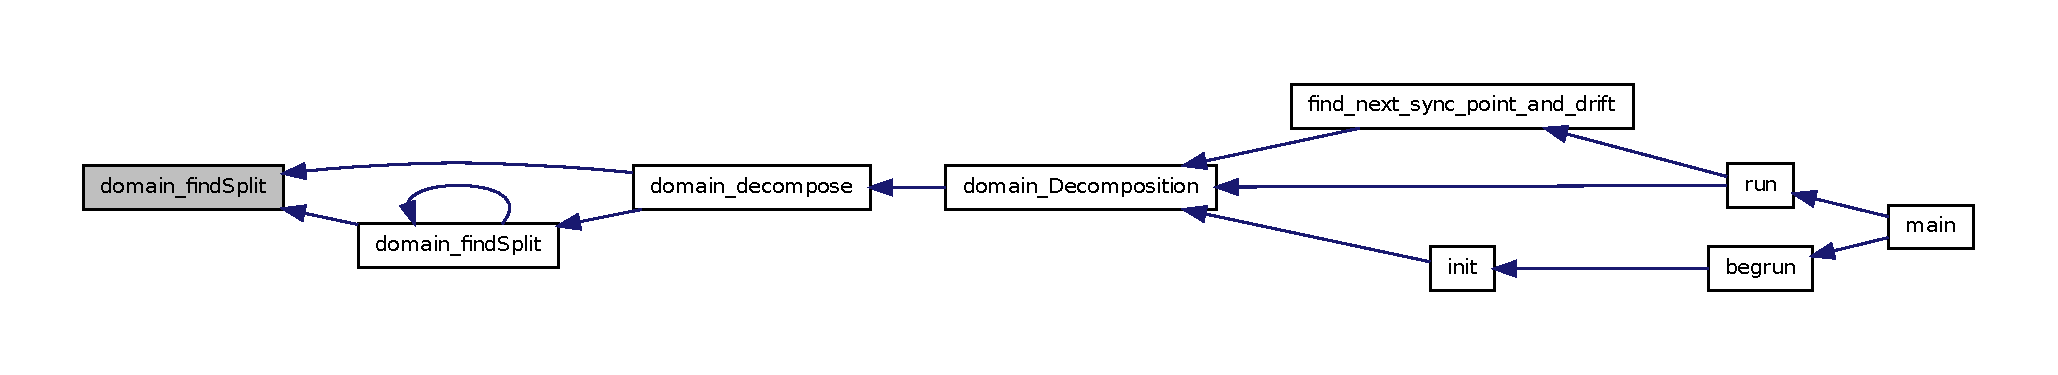
\includegraphics[width=400pt]{domain_8c_a412d5d8810751249cc8dcd9e219e4e57_icgraph}
\end{center}
\end{figure}


\hypertarget{domain_8c_a89c54187117b91d4270a4f0c406ce2ba}{
\index{domain.c@{domain.c}!domain\_\-shiftSplit@{domain\_\-shiftSplit}}
\index{domain\_\-shiftSplit@{domain\_\-shiftSplit}!domain.c@{domain.c}}
\subsubsection[{domain\_\-shiftSplit}]{\setlength{\rightskip}{0pt plus 5cm}void domain\_\-shiftSplit (
\begin{DoxyParamCaption}
\item[{void}]{}
\end{DoxyParamCaption}
)}}
\label{domain_8c_a89c54187117b91d4270a4f0c406ce2ba}
This function tries to improve the domain decomposition found by \hyperlink{domain_8c_a412d5d8810751249cc8dcd9e219e4e57}{domain\_\-findSplit()} with respect to work-\/load balance. To this end, the boundaries in the existing domain-\/split solution (which was found by trying to balance the particle load) are shifted as long as this leads to better work-\/load while still remaining within the allowed memory-\/imbalance constraints. 

Definition at line 447 of file domain.c.



References dmax(), DomainCount, DomainCountSph, DomainEndList, DomainStartList, DomainTask, DomainWork, list\_\-load, list\_\-loadsph, list\_\-work, maxload, maxloadsph, NTask, and NTopleaves.



Referenced by domain\_\-decompose().




\begin{DoxyCode}
{
  int i, task, iter = 0, moved;
  double maxw, newmaxw;

  for(task = 0; task < NTask; task++)
    list_work[task] = 0;

  for(i = 0; i < NTopleaves; i++)
    list_work[DomainTask[i]] += DomainWork[i];

  do
    {
      for(task = 0, moved = 0; task < NTask - 1; task++)
        {
          maxw = dmax(list_work[task], list_work[task + 1]);

          if(list_work[task] < list_work[task + 1])
            {
              newmaxw = dmax(list_work[task] + DomainWork[DomainStartList[task + 
      1]],
                             list_work[task + 1] - DomainWork[DomainStartList[tas
      k + 1]]);
              if(newmaxw <= maxw)
                {
                  if(list_load[task] + DomainCount[DomainStartList[task + 1]] <= 
      maxload)
                    {
                      if(list_loadsph[task] + DomainCountSph[DomainStartList[task
       + 1]] > maxloadsph)
                        continue;

                      /* ok, we can move one domain cell from right to left */
                      list_work[task] += DomainWork[DomainStartList[task + 1]];
                      list_load[task] += DomainCount[DomainStartList[task + 1]];
                      list_loadsph[task] += DomainCountSph[DomainStartList[task +
       1]];
                      list_work[task + 1] -= DomainWork[DomainStartList[task + 1]
      ];
                      list_load[task + 1] -= DomainCount[DomainStartList[task + 1
      ]];
                      list_loadsph[task + 1] -= DomainCountSph[DomainStartList[ta
      sk + 1]];

                      DomainTask[DomainStartList[task + 1]] = task;
                      DomainStartList[task + 1] += 1;
                      DomainEndList[task] += 1;

                      moved++;
                    }
                }
            }
          else
            {
              newmaxw = dmax(list_work[task] - DomainWork[DomainEndList[task]],
                             list_work[task + 1] + DomainWork[DomainEndList[task]
      ]);
              if(newmaxw <= maxw)
                {
                  if(list_load[task + 1] + DomainCount[DomainEndList[task]] <= 
      maxload)
                    {
                      if(list_loadsph[task + 1] + DomainCountSph[DomainEndList[ta
      sk]] > maxloadsph)
                        continue;

                      /* ok, we can move one domain cell from left to right */
                      list_work[task] -= DomainWork[DomainEndList[task]];
                      list_load[task] -= DomainCount[DomainEndList[task]];
                      list_loadsph[task] -= DomainCountSph[DomainEndList[task]];
                      list_work[task + 1] += DomainWork[DomainEndList[task]];
                      list_load[task + 1] += DomainCount[DomainEndList[task]];
                      list_loadsph[task + 1] += DomainCountSph[DomainEndList[task
      ]];

                      DomainTask[DomainEndList[task]] = task + 1;
                      DomainEndList[task] -= 1;
                      DomainStartList[task + 1] -= 1;

                      moved++;
                    }
                }

            }
        }

      iter++;
    }
  while(moved > 0 && iter < 10 * NTopleaves);
}
\end{DoxyCode}




Here is the call graph for this function:\nopagebreak
\begin{figure}[H]
\begin{center}
\leavevmode
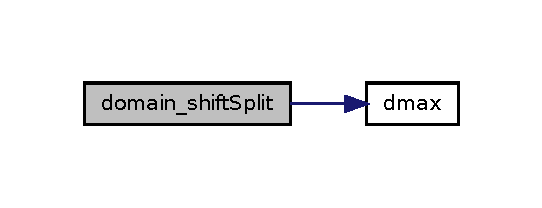
\includegraphics[width=260pt]{domain_8c_a89c54187117b91d4270a4f0c406ce2ba_cgraph}
\end{center}
\end{figure}




Here is the caller graph for this function:\nopagebreak
\begin{figure}[H]
\begin{center}
\leavevmode
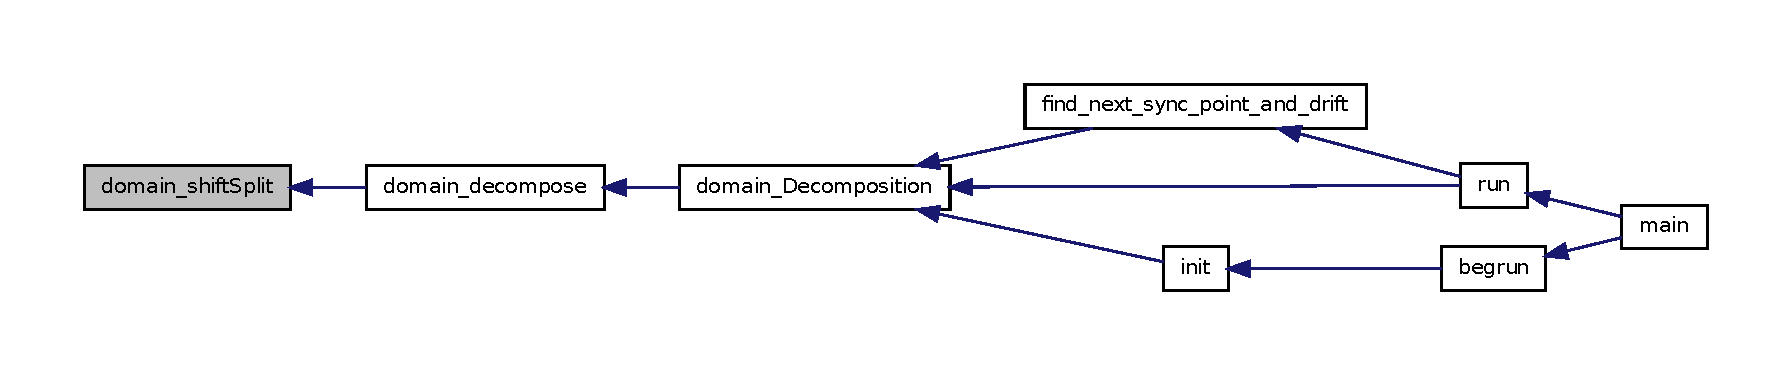
\includegraphics[width=400pt]{domain_8c_a89c54187117b91d4270a4f0c406ce2ba_icgraph}
\end{center}
\end{figure}


\hypertarget{domain_8c_a25aada0d3751c2afd2a376151d1d917e}{
\index{domain.c@{domain.c}!domain\_\-sumCost@{domain\_\-sumCost}}
\index{domain\_\-sumCost@{domain\_\-sumCost}!domain.c@{domain.c}}
\subsubsection[{domain\_\-sumCost}]{\setlength{\rightskip}{0pt plus 5cm}void domain\_\-sumCost (
\begin{DoxyParamCaption}
\item[{void}]{}
\end{DoxyParamCaption}
)}}
\label{domain_8c_a25aada0d3751c2afd2a376151d1d917e}
This routine bins the particles onto the domain-\/grid, i.e. it sums up the total number of particles and the total amount of work in each of the domain-\/cells. This information forms the basis for the actual decision on the adopted domain decomposition. 

Definition at line 786 of file domain.c.



References topnode\_\-data::Daughter, domain\_\-walktoptree(), DomainCount, DomainCountSph, DomainWork, particle\_\-data::GravCost, Key, topnode\_\-data::Leaf, NTopleaves, NTopnodes, NumPart, P, topnode\_\-data::StartKey, ThisTask, and TopNodes.



Referenced by domain\_\-decompose().




\begin{DoxyCode}
{
  int i, n, no;
  double *local_DomainWork;
  int *local_DomainCount;
  int *local_DomainCountSph;

  local_DomainWork = malloc(NTopnodes * sizeof(double));
  local_DomainCount = malloc(NTopnodes * sizeof(int));
  local_DomainCountSph = malloc(NTopnodes * sizeof(int));



  NTopleaves = 0;

  domain_walktoptree(0);

  for(i = 0; i < NTopleaves; i++)
    {
      local_DomainWork[i] = 0;
      local_DomainCount[i] = 0;
      local_DomainCountSph[i] = 0;
    }

  if(ThisTask == 0)
    printf("NTopleaves= %d\n", NTopleaves);

  for(n = 0; n < NumPart; n++)
    {
      no = 0;

      while(TopNodes[no].Daughter >= 0)
        no = TopNodes[no].Daughter + (Key[n] - TopNodes[no].StartKey) / (
      TopNodes[no].Size / 8);

      no = TopNodes[no].Leaf;

      if(P[n].Ti_endstep > P[n].Ti_begstep)
        local_DomainWork[no] += (1.0 + P[n].GravCost) / (P[n].Ti_endstep - P[n].T
      i_begstep);
      else
        local_DomainWork[no] += (1.0 + P[n].GravCost);

      local_DomainCount[no] += 1;
      if(P[n].Type == 0)
        local_DomainCountSph[no] += 1;
    }

  MPI_Allreduce(local_DomainWork, DomainWork, NTopleaves, MPI_DOUBLE, MPI_SUM, MP
      I_COMM_WORLD);
  MPI_Allreduce(local_DomainCount, DomainCount, NTopleaves, MPI_INT, MPI_SUM, MPI
      _COMM_WORLD);
  MPI_Allreduce(local_DomainCountSph, DomainCountSph, NTopleaves, MPI_INT, MPI_SU
      M, MPI_COMM_WORLD);


  free(local_DomainCountSph);
  free(local_DomainCount);
  free(local_DomainWork);
}
\end{DoxyCode}




Here is the call graph for this function:\nopagebreak
\begin{figure}[H]
\begin{center}
\leavevmode
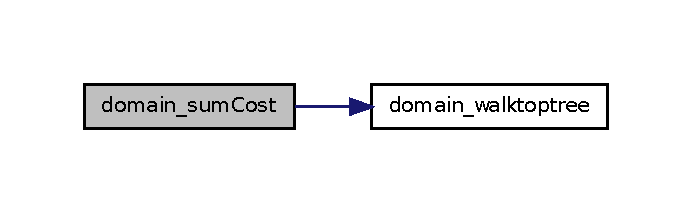
\includegraphics[width=332pt]{domain_8c_a25aada0d3751c2afd2a376151d1d917e_cgraph}
\end{center}
\end{figure}




Here is the caller graph for this function:\nopagebreak
\begin{figure}[H]
\begin{center}
\leavevmode
\includegraphics[width=400pt]{domain_8c_a25aada0d3751c2afd2a376151d1d917e_icgraph}
\end{center}
\end{figure}


\hypertarget{domain_8c_a606de536756a67ad8f79f1135009195e}{
\index{domain.c@{domain.c}!domain\_\-topsplit@{domain\_\-topsplit}}
\index{domain\_\-topsplit@{domain\_\-topsplit}!domain.c@{domain.c}}
\subsubsection[{domain\_\-topsplit}]{\setlength{\rightskip}{0pt plus 5cm}void domain\_\-topsplit (
\begin{DoxyParamCaption}
\item[{int}]{ node, }
\item[{{\bf peanokey}}]{ startkey}
\end{DoxyParamCaption}
)}}
\label{domain_8c_a606de536756a67ad8f79f1135009195e}
This function is responsible for constructing the global top-\/level tree segments. Starting from a joint list of all local top-\/level segments, in which mulitple occurences of the same spatial segment have been combined, a segment is subdivided into 8 pieces recursively until the number of particles in each segment has fallen below All.TotNumPart / (TOPNODEFACTOR $\ast$ NTask). 

$<$ Maximum number of nodes in the top-\/level tree used for domain decomposition 



Definition at line 1049 of file domain.c.



References All, topnode\_\-data::Blocks, topnode\_\-exchange::Count, topnode\_\-data::Count, topnode\_\-data::Daughter, domain\_\-topsplit(), endrun(), MAXTOPNODES, NTask, NTopnodes, topnode\_\-data::Pstart, topnode\_\-data::Size, topnode\_\-exchange::Startkey, topnode\_\-data::StartKey, ThisTask, toplist, TOPNODEFACTOR, TopNodes, and global\_\-data\_\-all\_\-processes::TotNumPart.



Referenced by domain\_\-determineTopTree(), and domain\_\-topsplit().




\begin{DoxyCode}
{
  int i, p, sub, bin;

  if(TopNodes[node].Size >= 8)
    {
      TopNodes[node].Daughter = NTopnodes;

      for(i = 0; i < 8; i++)
        {
          if(NTopnodes < MAXTOPNODES)
            {
              sub = TopNodes[node].Daughter + i;
              TopNodes[sub].Size = TopNodes[node].Size / 8;
              TopNodes[sub].Count = 0;
              TopNodes[sub].Blocks = 0;
              TopNodes[sub].Daughter = -1;
              TopNodes[sub].StartKey = startkey + i * TopNodes[sub].Size;
              TopNodes[sub].Pstart = TopNodes[node].Pstart;
              NTopnodes++;
            }
          else
            {
              printf("Task=%d: We are out of Topnodes. Increasing the constant MA
      XTOPNODES might help.\n",
                     ThisTask);
              fflush(stdout);
              endrun(137213);
            }
        }

      for(p = TopNodes[node].Pstart; p < TopNodes[node].Pstart + TopNodes[node].
      Blocks; p++)
        {
          bin = (toplist[p].Startkey - startkey) / (TopNodes[node].Size / 8);
          sub = TopNodes[node].Daughter + bin;

          if(bin < 0 || bin > 7)
            endrun(77);

          if(TopNodes[sub].Blocks == 0)
            TopNodes[sub].Pstart = p;

          TopNodes[sub].Count += toplist[p].Count;
          TopNodes[sub].Blocks++;
        }

      for(i = 0; i < 8; i++)
        {
          sub = TopNodes[node].Daughter + i;
          if(TopNodes[sub].Count > All.TotNumPart / (TOPNODEFACTOR * NTask))
            domain_topsplit(sub, TopNodes[sub].StartKey);
        }
    }
}
\end{DoxyCode}




Here is the call graph for this function:\nopagebreak
\begin{figure}[H]
\begin{center}
\leavevmode
\includegraphics[width=400pt]{domain_8c_a606de536756a67ad8f79f1135009195e_cgraph}
\end{center}
\end{figure}




Here is the caller graph for this function:\nopagebreak
\begin{figure}[H]
\begin{center}
\leavevmode
\includegraphics[width=400pt]{domain_8c_a606de536756a67ad8f79f1135009195e_icgraph}
\end{center}
\end{figure}


\hypertarget{domain_8c_aa5001f9be833c4673392b40e7be3a421}{
\index{domain.c@{domain.c}!domain\_\-topsplit\_\-local@{domain\_\-topsplit\_\-local}}
\index{domain\_\-topsplit\_\-local@{domain\_\-topsplit\_\-local}!domain.c@{domain.c}}
\subsubsection[{domain\_\-topsplit\_\-local}]{\setlength{\rightskip}{0pt plus 5cm}void domain\_\-topsplit\_\-local (
\begin{DoxyParamCaption}
\item[{int}]{ node, }
\item[{{\bf peanokey}}]{ startkey}
\end{DoxyParamCaption}
)}}
\label{domain_8c_aa5001f9be833c4673392b40e7be3a421}
This function is responsible for constructing the local top-\/level Peano-\/Hilbert segments. A segment is cut into 8 pieces recursively until the number of particles in the segment has fallen below All.TotNumPart / (TOPNODEFACTOR $\ast$ NTask $\ast$ NTask). 

$<$ Maximum number of nodes in the top-\/level tree used for domain decomposition 



Definition at line 982 of file domain.c.



References All, topnode\_\-exchange::Count, topnode\_\-data::Count, topnode\_\-data::Daughter, domain\_\-topsplit\_\-local(), endrun(), KeySorted, MAXTOPNODES, NTask, NTopnodes, topnode\_\-data::Pstart, topnode\_\-data::Size, topnode\_\-data::StartKey, ThisTask, TOPNODEFACTOR, TopNodes, and global\_\-data\_\-all\_\-processes::TotNumPart.



Referenced by domain\_\-determineTopTree(), and domain\_\-topsplit\_\-local().




\begin{DoxyCode}
{
  int i, p, sub, bin;

  if(TopNodes[node].Size >= 8)
    {
      TopNodes[node].Daughter = NTopnodes;

      for(i = 0; i < 8; i++)
        {
          if(NTopnodes < MAXTOPNODES)
            {
              sub = TopNodes[node].Daughter + i;
              TopNodes[sub].Size = TopNodes[node].Size / 8;
              TopNodes[sub].Count = 0;
              TopNodes[sub].Daughter = -1;
              TopNodes[sub].StartKey = startkey + i * TopNodes[sub].Size;
              TopNodes[sub].Pstart = TopNodes[node].Pstart;

              NTopnodes++;
            }
          else
            {
              printf("task=%d: We are out of Topnodes. Increasing the constant MA
      XTOPNODES might help.\n",
                     ThisTask);
              fflush(stdout);
              endrun(13213);
            }
        }

      for(p = TopNodes[node].Pstart; p < TopNodes[node].Pstart + TopNodes[node].
      Count; p++)
        {
          bin = (KeySorted[p] - startkey) / (TopNodes[node].Size / 8);

          if(bin < 0 || bin > 7)
            {
              printf("task=%d: something odd has happened here. bin=%d\n", 
      ThisTask, bin);
              fflush(stdout);
              endrun(13123123);
            }

          sub = TopNodes[node].Daughter + bin;

          if(TopNodes[sub].Count == 0)
            TopNodes[sub].Pstart = p;

          TopNodes[sub].Count++;
        }

      for(i = 0; i < 8; i++)
        {
          sub = TopNodes[node].Daughter + i;
          if(TopNodes[sub].Count > All.TotNumPart / (TOPNODEFACTOR * NTask * 
      NTask))
            domain_topsplit_local(sub, TopNodes[sub].StartKey);
        }
    }
}
\end{DoxyCode}




Here is the call graph for this function:\nopagebreak
\begin{figure}[H]
\begin{center}
\leavevmode
\includegraphics[width=400pt]{domain_8c_aa5001f9be833c4673392b40e7be3a421_cgraph}
\end{center}
\end{figure}




Here is the caller graph for this function:\nopagebreak
\begin{figure}[H]
\begin{center}
\leavevmode
\includegraphics[width=400pt]{domain_8c_aa5001f9be833c4673392b40e7be3a421_icgraph}
\end{center}
\end{figure}


\hypertarget{domain_8c_a9b1062a5c460164de378d5e8c45736c4}{
\index{domain.c@{domain.c}!domain\_\-walktoptree@{domain\_\-walktoptree}}
\index{domain\_\-walktoptree@{domain\_\-walktoptree}!domain.c@{domain.c}}
\subsubsection[{domain\_\-walktoptree}]{\setlength{\rightskip}{0pt plus 5cm}void domain\_\-walktoptree (
\begin{DoxyParamCaption}
\item[{int}]{ no}
\end{DoxyParamCaption}
)}}
\label{domain_8c_a9b1062a5c460164de378d5e8c45736c4}
This function walks the global top tree in order to establish the number of leaves it has. These leaves are distributed to different processors. 

Definition at line 765 of file domain.c.



References topnode\_\-data::Leaf, NTopleaves, and TopNodes.



Referenced by domain\_\-sumCost().




\begin{DoxyCode}
{
  int i;

  if(TopNodes[no].Daughter == -1)
    {
      TopNodes[no].Leaf = NTopleaves;
      NTopleaves++;
    }
  else
    {
      for(i = 0; i < 8; i++)
        domain_walktoptree(TopNodes[no].Daughter + i);
    }
}
\end{DoxyCode}




Here is the caller graph for this function:\nopagebreak
\begin{figure}[H]
\begin{center}
\leavevmode
\includegraphics[width=400pt]{domain_8c_a9b1062a5c460164de378d5e8c45736c4_icgraph}
\end{center}
\end{figure}




\subsection{Variable Documentation}
\hypertarget{domain_8c_af3343810478135e16ac72ea1f0172cd6}{
\index{domain.c@{domain.c}!list\_\-load@{list\_\-load}}
\index{list\_\-load@{list\_\-load}!domain.c@{domain.c}}
\subsubsection[{list\_\-load}]{\setlength{\rightskip}{0pt plus 5cm}int$\ast$ {\bf list\_\-load}\hspace{0.3cm}{\ttfamily  \mbox{[}static\mbox{]}}}}
\label{domain_8c_af3343810478135e16ac72ea1f0172cd6}


Definition at line 41 of file domain.c.



Referenced by domain\_\-decompose(), domain\_\-Decomposition(), domain\_\-findSplit(), and domain\_\-shiftSplit().

\hypertarget{domain_8c_a97ae02d63ef3ac017dcbaea0d3b4dda4}{
\index{domain.c@{domain.c}!list\_\-loadsph@{list\_\-loadsph}}
\index{list\_\-loadsph@{list\_\-loadsph}!domain.c@{domain.c}}
\subsubsection[{list\_\-loadsph}]{\setlength{\rightskip}{0pt plus 5cm}int$\ast$ {\bf list\_\-loadsph}\hspace{0.3cm}{\ttfamily  \mbox{[}static\mbox{]}}}}
\label{domain_8c_a97ae02d63ef3ac017dcbaea0d3b4dda4}


Definition at line 42 of file domain.c.



Referenced by domain\_\-Decomposition(), domain\_\-findSplit(), and domain\_\-shiftSplit().

\hypertarget{domain_8c_a9819cd512382caee762325ea86f4b221}{
\index{domain.c@{domain.c}!list\_\-N\_\-gas@{list\_\-N\_\-gas}}
\index{list\_\-N\_\-gas@{list\_\-N\_\-gas}!domain.c@{domain.c}}
\subsubsection[{list\_\-N\_\-gas}]{\setlength{\rightskip}{0pt plus 5cm}int$\ast$ {\bf list\_\-N\_\-gas}\hspace{0.3cm}{\ttfamily  \mbox{[}static\mbox{]}}}}
\label{domain_8c_a9819cd512382caee762325ea86f4b221}


Definition at line 40 of file domain.c.



Referenced by domain\_\-decompose(), domain\_\-Decomposition(), and domain\_\-findExchangeNumbers().

\hypertarget{domain_8c_a040694ce8b01a0b994df96d39588813a}{
\index{domain.c@{domain.c}!list\_\-NumPart@{list\_\-NumPart}}
\index{list\_\-NumPart@{list\_\-NumPart}!domain.c@{domain.c}}
\subsubsection[{list\_\-NumPart}]{\setlength{\rightskip}{0pt plus 5cm}int$\ast$ {\bf list\_\-NumPart}\hspace{0.3cm}{\ttfamily  \mbox{[}static\mbox{]}}}}
\label{domain_8c_a040694ce8b01a0b994df96d39588813a}


Definition at line 39 of file domain.c.



Referenced by domain\_\-decompose(), domain\_\-Decomposition(), and domain\_\-findExchangeNumbers().

\hypertarget{domain_8c_ad25e64ba07e1ed5350cceeab486c6f4a}{
\index{domain.c@{domain.c}!list\_\-work@{list\_\-work}}
\index{list\_\-work@{list\_\-work}!domain.c@{domain.c}}
\subsubsection[{list\_\-work}]{\setlength{\rightskip}{0pt plus 5cm}double$\ast$ {\bf list\_\-work}\hspace{0.3cm}{\ttfamily  \mbox{[}static\mbox{]}}}}
\label{domain_8c_ad25e64ba07e1ed5350cceeab486c6f4a}


Definition at line 43 of file domain.c.



Referenced by domain\_\-decompose(), domain\_\-Decomposition(), and domain\_\-shiftSplit().

\hypertarget{domain_8c_a394783c89866b4e48255038384f9539b}{
\index{domain.c@{domain.c}!local\_\-toGo@{local\_\-toGo}}
\index{local\_\-toGo@{local\_\-toGo}!domain.c@{domain.c}}
\subsubsection[{local\_\-toGo}]{\setlength{\rightskip}{0pt plus 5cm}int$\ast$ {\bf local\_\-toGo}\hspace{0.3cm}{\ttfamily  \mbox{[}static\mbox{]}}}}
\label{domain_8c_a394783c89866b4e48255038384f9539b}


Definition at line 38 of file domain.c.



Referenced by domain\_\-countToGo(), and domain\_\-Decomposition().

\hypertarget{domain_8c_a119a354c6c46ee11fdb9c7ad131b787a}{
\index{domain.c@{domain.c}!local\_\-toGoSph@{local\_\-toGoSph}}
\index{local\_\-toGoSph@{local\_\-toGoSph}!domain.c@{domain.c}}
\subsubsection[{local\_\-toGoSph}]{\setlength{\rightskip}{0pt plus 5cm}int $\ast$ {\bf local\_\-toGoSph}\hspace{0.3cm}{\ttfamily  \mbox{[}static\mbox{]}}}}
\label{domain_8c_a119a354c6c46ee11fdb9c7ad131b787a}


Definition at line 38 of file domain.c.



Referenced by domain\_\-countToGo(), and domain\_\-Decomposition().

\hypertarget{domain_8c_ac54707073f160b11ee4ba864066487c3}{
\index{domain.c@{domain.c}!maxload@{maxload}}
\index{maxload@{maxload}!domain.c@{domain.c}}
\subsubsection[{maxload}]{\setlength{\rightskip}{0pt plus 5cm}long long {\bf maxload}\hspace{0.3cm}{\ttfamily  \mbox{[}static\mbox{]}}}}
\label{domain_8c_ac54707073f160b11ee4ba864066487c3}


Definition at line 45 of file domain.c.



Referenced by domain\_\-decompose(), domain\_\-Decomposition(), domain\_\-findSplit(), and domain\_\-shiftSplit().

\hypertarget{domain_8c_afa6a98969329aca0189182e060a2834e}{
\index{domain.c@{domain.c}!maxloadsph@{maxloadsph}}
\index{maxloadsph@{maxloadsph}!domain.c@{domain.c}}
\subsubsection[{maxloadsph}]{\setlength{\rightskip}{0pt plus 5cm}long long {\bf maxloadsph}\hspace{0.3cm}{\ttfamily  \mbox{[}static\mbox{]}}}}
\label{domain_8c_afa6a98969329aca0189182e060a2834e}


Definition at line 45 of file domain.c.



Referenced by domain\_\-Decomposition(), domain\_\-findSplit(), and domain\_\-shiftSplit().

\hypertarget{domain_8c_a52aefc67245e1a334c311a420f89130c}{
\index{domain.c@{domain.c}!toGo@{toGo}}
\index{toGo@{toGo}!domain.c@{domain.c}}
\subsubsection[{toGo}]{\setlength{\rightskip}{0pt plus 5cm}int$\ast$ {\bf toGo}\hspace{0.3cm}{\ttfamily  \mbox{[}static\mbox{]}}}}
\label{domain_8c_a52aefc67245e1a334c311a420f89130c}
toGo\mbox{[}task$\ast$NTask + partner\mbox{]} gives the number of particles in task 'task' that have to go to task 'partner' 

Definition at line 37 of file domain.c.



Referenced by domain\_\-countToGo(), domain\_\-decompose(), domain\_\-Decomposition(), and domain\_\-findExchangeNumbers().

\hypertarget{domain_8c_af00bb52ac4aa095d4d6daac54833675f}{
\index{domain.c@{domain.c}!toGoSph@{toGoSph}}
\index{toGoSph@{toGoSph}!domain.c@{domain.c}}
\subsubsection[{toGoSph}]{\setlength{\rightskip}{0pt plus 5cm}int $\ast$ {\bf toGoSph}\hspace{0.3cm}{\ttfamily  \mbox{[}static\mbox{]}}}}
\label{domain_8c_af00bb52ac4aa095d4d6daac54833675f}


Definition at line 37 of file domain.c.



Referenced by domain\_\-countToGo(), domain\_\-decompose(), domain\_\-Decomposition(), and domain\_\-findExchangeNumbers().

\hypertarget{domain_8c_aa4d05cc74afde41e1777c117c9103471}{
\index{domain.c@{domain.c}!toplist@{toplist}}
\index{toplist@{toplist}!domain.c@{domain.c}}
\subsubsection[{toplist}]{\setlength{\rightskip}{0pt plus 5cm}struct {\bf topnode\_\-exchange}
 $\ast$ {\bf toplist}\hspace{0.3cm}{\ttfamily  \mbox{[}static\mbox{]}}}}
\label{domain_8c_aa4d05cc74afde41e1777c117c9103471}


Referenced by domain\_\-determineTopTree(), and domain\_\-topsplit().

\hypertarget{domain_8c_a62244375ee3d9bdb3f7428a58de42085}{
\index{domain.c@{domain.c}!toplist\_\-local@{toplist\_\-local}}
\index{toplist\_\-local@{toplist\_\-local}!domain.c@{domain.c}}
\subsubsection[{toplist\_\-local}]{\setlength{\rightskip}{0pt plus 5cm}struct {\bf topnode\_\-exchange} $\ast$ {\bf toplist\_\-local}\hspace{0.3cm}{\ttfamily  \mbox{[}static\mbox{]}}}}
\label{domain_8c_a62244375ee3d9bdb3f7428a58de42085}


Referenced by domain\_\-determineTopTree().


\hypertarget{driftfac_8c}{
\section{driftfac.c File Reference}
\label{driftfac_8c}\index{driftfac.c@{driftfac.c}}
}


compute loop-\/up tables for prefactors in cosmological integration  


{\ttfamily \#include $<$stdio.h$>$}\par
{\ttfamily \#include $<$stdlib.h$>$}\par
{\ttfamily \#include $<$string.h$>$}\par
{\ttfamily \#include $<$math.h$>$}\par
{\ttfamily \#include $<$mpi.h$>$}\par
{\ttfamily \#include $<$gsl/gsl\_\-math.h$>$}\par
{\ttfamily \#include $<$gsl/gsl\_\-integration.h$>$}\par
{\ttfamily \#include \char`\"{}allvars.h\char`\"{}}\par
{\ttfamily \#include \char`\"{}proto.h\char`\"{}}\par
Include dependency graph for driftfac.c:\nopagebreak
\begin{figure}[H]
\begin{center}
\leavevmode
\includegraphics[width=400pt]{driftfac_8c__incl}
\end{center}
\end{figure}
\subsection*{Defines}
\begin{DoxyCompactItemize}
\item 
\#define \hyperlink{driftfac_8c_a2adb5d14857fdbea8ba352245450e52a}{WORKSIZE}~100000
\end{DoxyCompactItemize}
\subsection*{Functions}
\begin{DoxyCompactItemize}
\item 
void \hyperlink{driftfac_8c_aea1f81063199abb9d89802b444098018}{init\_\-drift\_\-table} (void)
\item 
double \hyperlink{driftfac_8c_adadb384299eb936596574417d4b6b28c}{get\_\-drift\_\-factor} (int time0, int time1)
\item 
double \hyperlink{driftfac_8c_a29057b821b850ab54b318d7339633059}{get\_\-gravkick\_\-factor} (int time0, int time1)
\item 
double \hyperlink{driftfac_8c_ace65dca1556185b12c7f22427724c90c}{get\_\-hydrokick\_\-factor} (int time0, int time1)
\item 
double \hyperlink{driftfac_8c_a8cb77fa18fd6b91a358bd0a9c04cbf2e}{drift\_\-integ} (double a, void $\ast$param)
\item 
double \hyperlink{driftfac_8c_a2eafe05fb12d7f9d954d5b501e186051}{gravkick\_\-integ} (double a, void $\ast$param)
\item 
double \hyperlink{driftfac_8c_a5ebdee2c7332bed6c1a8994ac3c38c0d}{hydrokick\_\-integ} (double a, void $\ast$param)
\item 
double \hyperlink{driftfac_8c_a9690d42f31f3e278745a9e19b5a0ec6f}{growthfactor\_\-integ} (double a, void $\ast$param)
\end{DoxyCompactItemize}
\subsection*{Variables}
\begin{DoxyCompactItemize}
\item 
static double \hyperlink{driftfac_8c_adf1795a43a5fd6de0a14b805094dac47}{logTimeBegin}
\item 
static double \hyperlink{driftfac_8c_a0e08a12787034f570c56ff664de37e2a}{logTimeMax}
\end{DoxyCompactItemize}


\subsection{Detailed Description}
compute loop-\/up tables for prefactors in cosmological integration 

Definition in file \hyperlink{driftfac_8c_source}{driftfac.c}.



\subsection{Define Documentation}
\hypertarget{driftfac_8c_a2adb5d14857fdbea8ba352245450e52a}{
\index{driftfac.c@{driftfac.c}!WORKSIZE@{WORKSIZE}}
\index{WORKSIZE@{WORKSIZE}!driftfac.c@{driftfac.c}}
\subsubsection[{WORKSIZE}]{\setlength{\rightskip}{0pt plus 5cm}\#define WORKSIZE~100000}}
\label{driftfac_8c_a2adb5d14857fdbea8ba352245450e52a}


Referenced by init\_\-drift\_\-table().



\subsection{Function Documentation}
\hypertarget{driftfac_8c_a8cb77fa18fd6b91a358bd0a9c04cbf2e}{
\index{driftfac.c@{driftfac.c}!drift\_\-integ@{drift\_\-integ}}
\index{drift\_\-integ@{drift\_\-integ}!driftfac.c@{driftfac.c}}
\subsubsection[{drift\_\-integ}]{\setlength{\rightskip}{0pt plus 5cm}double drift\_\-integ (
\begin{DoxyParamCaption}
\item[{double}]{ a, }
\item[{void $\ast$}]{ param}
\end{DoxyParamCaption}
)}}
\label{driftfac_8c_a8cb77fa18fd6b91a358bd0a9c04cbf2e}
Integration kernel for drift factor computation. 

Definition at line 179 of file driftfac.c.



References All, global\_\-data\_\-all\_\-processes::Hubble, global\_\-data\_\-all\_\-processes::Omega0, and global\_\-data\_\-all\_\-processes::OmegaLambda.




\begin{DoxyCode}
{
  double h;

  h = All.Omega0 / (a * a * a) + (1 - All.Omega0 - All.OmegaLambda) / (a * a) + 
      All.OmegaLambda;
  h = All.Hubble * sqrt(h);

  return 1 / (h * a * a * a);
}
\end{DoxyCode}


\hypertarget{driftfac_8c_adadb384299eb936596574417d4b6b28c}{
\index{driftfac.c@{driftfac.c}!get\_\-drift\_\-factor@{get\_\-drift\_\-factor}}
\index{get\_\-drift\_\-factor@{get\_\-drift\_\-factor}!driftfac.c@{driftfac.c}}
\subsubsection[{get\_\-drift\_\-factor}]{\setlength{\rightskip}{0pt plus 5cm}double get\_\-drift\_\-factor (
\begin{DoxyParamCaption}
\item[{int}]{ time0, }
\item[{int}]{ time1}
\end{DoxyParamCaption}
)}}
\label{driftfac_8c_adadb384299eb936596574417d4b6b28c}
This function integrates the cosmological prefactor for a drift step between time0 and time1. The value returned is $\ast$ \[ \int_{a_0}^{a_1} \frac{{\rm d}a}{H(a)} * \] 

$<$ length of the lookup table used to hold the drift and kick factors

$<$ length of the lookup table used to hold the drift and kick factors

$<$ length of the lookup table used to hold the drift and kick factors

$<$ length of the lookup table used to hold the drift and kick factors

$<$ length of the lookup table used to hold the drift and kick factors

$<$ length of the lookup table used to hold the drift and kick factors 



Definition at line 67 of file driftfac.c.



References All, DRIFT\_\-TABLE\_\-LENGTH, DriftTable, logTimeBegin, logTimeMax, and global\_\-data\_\-all\_\-processes::Timebase\_\-interval.



Referenced by move\_\-particles().




\begin{DoxyCode}
{
  double a1, a2, df1, df2, u1, u2;
  int i1, i2;

  /* note: will only be called for cosmological integration */

  a1 = logTimeBegin + time0 * All.Timebase_interval;
  a2 = logTimeBegin + time1 * All.Timebase_interval;

  u1 = (a1 - logTimeBegin) / (logTimeMax - logTimeBegin) * DRIFT_TABLE_LENGTH;
  i1 = (int) u1;
  if(i1 >= DRIFT_TABLE_LENGTH)
    i1 = DRIFT_TABLE_LENGTH - 1;

  if(i1 <= 1)
    df1 = u1 * DriftTable[0];
  else
    df1 = DriftTable[i1 - 1] + (DriftTable[i1] - DriftTable[i1 - 1]) * (u1 - i1);
      


  u2 = (a2 - logTimeBegin) / (logTimeMax - logTimeBegin) * DRIFT_TABLE_LENGTH;
  i2 = (int) u2;
  if(i2 >= DRIFT_TABLE_LENGTH)
    i2 = DRIFT_TABLE_LENGTH - 1;

  if(i2 <= 1)
    df2 = u2 * DriftTable[0];
  else
    df2 = DriftTable[i2 - 1] + (DriftTable[i2] - DriftTable[i2 - 1]) * (u2 - i2);
      

  return df2 - df1;
}
\end{DoxyCode}




Here is the caller graph for this function:\nopagebreak
\begin{figure}[H]
\begin{center}
\leavevmode
\includegraphics[width=400pt]{driftfac_8c_adadb384299eb936596574417d4b6b28c_icgraph}
\end{center}
\end{figure}


\hypertarget{driftfac_8c_a29057b821b850ab54b318d7339633059}{
\index{driftfac.c@{driftfac.c}!get\_\-gravkick\_\-factor@{get\_\-gravkick\_\-factor}}
\index{get\_\-gravkick\_\-factor@{get\_\-gravkick\_\-factor}!driftfac.c@{driftfac.c}}
\subsubsection[{get\_\-gravkick\_\-factor}]{\setlength{\rightskip}{0pt plus 5cm}double get\_\-gravkick\_\-factor (
\begin{DoxyParamCaption}
\item[{int}]{ time0, }
\item[{int}]{ time1}
\end{DoxyParamCaption}
)}}
\label{driftfac_8c_a29057b821b850ab54b318d7339633059}
This function integrates the cosmological prefactor for a kick step of the gravitational force. 

$<$ length of the lookup table used to hold the drift and kick factors

$<$ length of the lookup table used to hold the drift and kick factors

$<$ length of the lookup table used to hold the drift and kick factors

$<$ length of the lookup table used to hold the drift and kick factors

$<$ length of the lookup table used to hold the drift and kick factors

$<$ length of the lookup table used to hold the drift and kick factors 



Definition at line 105 of file driftfac.c.



References All, DRIFT\_\-TABLE\_\-LENGTH, GravKickTable, logTimeBegin, logTimeMax, and global\_\-data\_\-all\_\-processes::Timebase\_\-interval.



Referenced by advance\_\-and\_\-find\_\-timesteps(), compute\_\-global\_\-quantities\_\-of\_\-system(), fill\_\-write\_\-buffer(), and move\_\-particles().




\begin{DoxyCode}
{
  double a1, a2, df1, df2, u1, u2;
  int i1, i2;

  /* note: will only be called for cosmological integration */

  a1 = logTimeBegin + time0 * All.Timebase_interval;
  a2 = logTimeBegin + time1 * All.Timebase_interval;

  u1 = (a1 - logTimeBegin) / (logTimeMax - logTimeBegin) * DRIFT_TABLE_LENGTH;
  i1 = (int) u1;
  if(i1 >= DRIFT_TABLE_LENGTH)
    i1 = DRIFT_TABLE_LENGTH - 1;

  if(i1 <= 1)
    df1 = u1 * GravKickTable[0];
  else
    df1 = GravKickTable[i1 - 1] + (GravKickTable[i1] - GravKickTable[i1 - 1]) * (
      u1 - i1);


  u2 = (a2 - logTimeBegin) / (logTimeMax - logTimeBegin) * DRIFT_TABLE_LENGTH;
  i2 = (int) u2;
  if(i2 >= DRIFT_TABLE_LENGTH)
    i2 = DRIFT_TABLE_LENGTH - 1;

  if(i2 <= 1)
    df2 = u2 * GravKickTable[0];
  else
    df2 = GravKickTable[i2 - 1] + (GravKickTable[i2] - GravKickTable[i2 - 1]) * (
      u2 - i2);

  return df2 - df1;
}
\end{DoxyCode}




Here is the caller graph for this function:\nopagebreak
\begin{figure}[H]
\begin{center}
\leavevmode
\includegraphics[width=400pt]{driftfac_8c_a29057b821b850ab54b318d7339633059_icgraph}
\end{center}
\end{figure}


\hypertarget{driftfac_8c_ace65dca1556185b12c7f22427724c90c}{
\index{driftfac.c@{driftfac.c}!get\_\-hydrokick\_\-factor@{get\_\-hydrokick\_\-factor}}
\index{get\_\-hydrokick\_\-factor@{get\_\-hydrokick\_\-factor}!driftfac.c@{driftfac.c}}
\subsubsection[{get\_\-hydrokick\_\-factor}]{\setlength{\rightskip}{0pt plus 5cm}double get\_\-hydrokick\_\-factor (
\begin{DoxyParamCaption}
\item[{int}]{ time0, }
\item[{int}]{ time1}
\end{DoxyParamCaption}
)}}
\label{driftfac_8c_ace65dca1556185b12c7f22427724c90c}
This function integrates the cosmological prefactor for a kick step of the hydrodynamical force. 

$<$ length of the lookup table used to hold the drift and kick factors

$<$ length of the lookup table used to hold the drift and kick factors

$<$ length of the lookup table used to hold the drift and kick factors

$<$ length of the lookup table used to hold the drift and kick factors

$<$ length of the lookup table used to hold the drift and kick factors

$<$ length of the lookup table used to hold the drift and kick factors 



Definition at line 142 of file driftfac.c.



References All, DRIFT\_\-TABLE\_\-LENGTH, HydroKickTable, logTimeBegin, logTimeMax, and global\_\-data\_\-all\_\-processes::Timebase\_\-interval.



Referenced by advance\_\-and\_\-find\_\-timesteps(), compute\_\-global\_\-quantities\_\-of\_\-system(), fill\_\-write\_\-buffer(), and move\_\-particles().




\begin{DoxyCode}
{
  double a1, a2, df1, df2, u1, u2;
  int i1, i2;

  /* note: will only be called for cosmological integration */

  a1 = logTimeBegin + time0 * All.Timebase_interval;
  a2 = logTimeBegin + time1 * All.Timebase_interval;

  u1 = (a1 - logTimeBegin) / (logTimeMax - logTimeBegin) * DRIFT_TABLE_LENGTH;
  i1 = (int) u1;
  if(i1 >= DRIFT_TABLE_LENGTH)
    i1 = DRIFT_TABLE_LENGTH - 1;

  if(i1 <= 1)
    df1 = u1 * HydroKickTable[0];
  else
    df1 = HydroKickTable[i1 - 1] + (HydroKickTable[i1] - HydroKickTable[i1 - 1]) 
      * (u1 - i1);


  u2 = (a2 - logTimeBegin) / (logTimeMax - logTimeBegin) * DRIFT_TABLE_LENGTH;
  i2 = (int) u2;
  if(i2 >= DRIFT_TABLE_LENGTH)
    i2 = DRIFT_TABLE_LENGTH - 1;

  if(i2 <= 1)
    df2 = u2 * HydroKickTable[0];
  else
    df2 = HydroKickTable[i2 - 1] + (HydroKickTable[i2] - HydroKickTable[i2 - 1]) 
      * (u2 - i2);

  return df2 - df1;
}
\end{DoxyCode}




Here is the caller graph for this function:\nopagebreak
\begin{figure}[H]
\begin{center}
\leavevmode
\includegraphics[width=400pt]{driftfac_8c_ace65dca1556185b12c7f22427724c90c_icgraph}
\end{center}
\end{figure}


\hypertarget{driftfac_8c_a2eafe05fb12d7f9d954d5b501e186051}{
\index{driftfac.c@{driftfac.c}!gravkick\_\-integ@{gravkick\_\-integ}}
\index{gravkick\_\-integ@{gravkick\_\-integ}!driftfac.c@{driftfac.c}}
\subsubsection[{gravkick\_\-integ}]{\setlength{\rightskip}{0pt plus 5cm}double gravkick\_\-integ (
\begin{DoxyParamCaption}
\item[{double}]{ a, }
\item[{void $\ast$}]{ param}
\end{DoxyParamCaption}
)}}
\label{driftfac_8c_a2eafe05fb12d7f9d954d5b501e186051}
Integration kernel for gravitational kick factor computation. 

Definition at line 191 of file driftfac.c.



References All, global\_\-data\_\-all\_\-processes::Hubble, global\_\-data\_\-all\_\-processes::Omega0, and global\_\-data\_\-all\_\-processes::OmegaLambda.




\begin{DoxyCode}
{
  double h;

  h = All.Omega0 / (a * a * a) + (1 - All.Omega0 - All.OmegaLambda) / (a * a) + 
      All.OmegaLambda;
  h = All.Hubble * sqrt(h);

  return 1 / (h * a * a);
}
\end{DoxyCode}


\hypertarget{driftfac_8c_a9690d42f31f3e278745a9e19b5a0ec6f}{
\index{driftfac.c@{driftfac.c}!growthfactor\_\-integ@{growthfactor\_\-integ}}
\index{growthfactor\_\-integ@{growthfactor\_\-integ}!driftfac.c@{driftfac.c}}
\subsubsection[{growthfactor\_\-integ}]{\setlength{\rightskip}{0pt plus 5cm}double growthfactor\_\-integ (
\begin{DoxyParamCaption}
\item[{double}]{ a, }
\item[{void $\ast$}]{ param}
\end{DoxyParamCaption}
)}}
\label{driftfac_8c_a9690d42f31f3e278745a9e19b5a0ec6f}


Definition at line 214 of file driftfac.c.



References All, global\_\-data\_\-all\_\-processes::Omega0, global\_\-data\_\-all\_\-processes::OmegaLambda, and pow().




\begin{DoxyCode}
{
  double s;

  s = All.Omega0 + (1 - All.Omega0 - All.OmegaLambda) * a + All.OmegaLambda * a *
       a * a;
  s = sqrt(s);

  return pow(sqrt(a) / s, 3);
}
\end{DoxyCode}




Here is the call graph for this function:\nopagebreak
\begin{figure}[H]
\begin{center}
\leavevmode
\includegraphics[width=258pt]{driftfac_8c_a9690d42f31f3e278745a9e19b5a0ec6f_cgraph}
\end{center}
\end{figure}


\hypertarget{driftfac_8c_a5ebdee2c7332bed6c1a8994ac3c38c0d}{
\index{driftfac.c@{driftfac.c}!hydrokick\_\-integ@{hydrokick\_\-integ}}
\index{hydrokick\_\-integ@{hydrokick\_\-integ}!driftfac.c@{driftfac.c}}
\subsubsection[{hydrokick\_\-integ}]{\setlength{\rightskip}{0pt plus 5cm}double hydrokick\_\-integ (
\begin{DoxyParamCaption}
\item[{double}]{ a, }
\item[{void $\ast$}]{ param}
\end{DoxyParamCaption}
)}}
\label{driftfac_8c_a5ebdee2c7332bed6c1a8994ac3c38c0d}
Integration kernel for hydrodynamical kick factor computation. 

$<$ adiabatic index of simulated gas 



Definition at line 204 of file driftfac.c.



References All, GAMMA\_\-MINUS1, global\_\-data\_\-all\_\-processes::Hubble, global\_\-data\_\-all\_\-processes::Omega0, global\_\-data\_\-all\_\-processes::OmegaLambda, and pow().




\begin{DoxyCode}
{
  double h;

  h = All.Omega0 / (a * a * a) + (1 - All.Omega0 - All.OmegaLambda) / (a * a) + 
      All.OmegaLambda;
  h = All.Hubble * sqrt(h);

  return 1 / (h * pow(a, 3 * GAMMA_MINUS1) * a);
}
\end{DoxyCode}




Here is the call graph for this function:\nopagebreak
\begin{figure}[H]
\begin{center}
\leavevmode
\includegraphics[width=244pt]{driftfac_8c_a5ebdee2c7332bed6c1a8994ac3c38c0d_cgraph}
\end{center}
\end{figure}


\hypertarget{driftfac_8c_aea1f81063199abb9d89802b444098018}{
\index{driftfac.c@{driftfac.c}!init\_\-drift\_\-table@{init\_\-drift\_\-table}}
\index{init\_\-drift\_\-table@{init\_\-drift\_\-table}!driftfac.c@{driftfac.c}}
\subsubsection[{init\_\-drift\_\-table}]{\setlength{\rightskip}{0pt plus 5cm}void init\_\-drift\_\-table (
\begin{DoxyParamCaption}
\item[{void}]{}
\end{DoxyParamCaption}
)}}
\label{driftfac_8c_aea1f81063199abb9d89802b444098018}
This function computes look-\/up tables for factors needed in cosmological integrations. The (simple) integrations are carried out with the GSL library. Separate factors are computed for the \char`\"{}drift\char`\"{}, and the gravitational and hydrodynamical \char`\"{}kicks\char`\"{}. The lookup-\/table is used for reasons of speed. 

$<$ length of the lookup table used to hold the drift and kick factors

$<$ length of the lookup table used to hold the drift and kick factors

$<$ length of the lookup table used to hold the drift and kick factors

$<$ length of the lookup table used to hold the drift and kick factors 



Definition at line 26 of file driftfac.c.



References All, DriftTable, GravKickTable, HydroKickTable, logTimeBegin, logTimeMax, global\_\-data\_\-all\_\-processes::TimeBegin, global\_\-data\_\-all\_\-processes::TimeMax, WORKSIZE, and workspace.



Referenced by begrun().




\begin{DoxyCode}
{
#define WORKSIZE 100000
  int i;
  double result, abserr;
  gsl_function F;
  gsl_integration_workspace *workspace;

  logTimeBegin = log(All.TimeBegin);
  logTimeMax = log(All.TimeMax);

  workspace = gsl_integration_workspace_alloc(WORKSIZE);

  for(i = 0; i < DRIFT_TABLE_LENGTH; i++)
    {
      F.function = &drift_integ;
      gsl_integration_qag(&F, exp(logTimeBegin), exp(logTimeBegin + ((logTimeMax 
      - logTimeBegin) / DRIFT_TABLE_LENGTH) * (i + 1)), 0,
                          1.0e-8, WORKSIZE, GSL_INTEG_GAUSS41, workspace, &result
      , &abserr);
      DriftTable[i] = result;


      F.function = &gravkick_integ;
      gsl_integration_qag(&F, exp(logTimeBegin), exp(logTimeBegin + ((logTimeMax 
      - logTimeBegin) / DRIFT_TABLE_LENGTH) * (i + 1)), 0,
                          1.0e-8, WORKSIZE, GSL_INTEG_GAUSS41, workspace, &result
      , &abserr);
      GravKickTable[i] = result;


      F.function = &hydrokick_integ;
      gsl_integration_qag(&F, exp(logTimeBegin), exp(logTimeBegin + ((logTimeMax 
      - logTimeBegin) / DRIFT_TABLE_LENGTH) * (i + 1)), 0,
                          1.0e-8, WORKSIZE, GSL_INTEG_GAUSS41, workspace, &result
      , &abserr);
      HydroKickTable[i] = result;
    }

  gsl_integration_workspace_free(workspace);
}
\end{DoxyCode}




Here is the caller graph for this function:\nopagebreak
\begin{figure}[H]
\begin{center}
\leavevmode
\includegraphics[width=328pt]{driftfac_8c_aea1f81063199abb9d89802b444098018_icgraph}
\end{center}
\end{figure}




\subsection{Variable Documentation}
\hypertarget{driftfac_8c_adf1795a43a5fd6de0a14b805094dac47}{
\index{driftfac.c@{driftfac.c}!logTimeBegin@{logTimeBegin}}
\index{logTimeBegin@{logTimeBegin}!driftfac.c@{driftfac.c}}
\subsubsection[{logTimeBegin}]{\setlength{\rightskip}{0pt plus 5cm}double {\bf logTimeBegin}\hspace{0.3cm}{\ttfamily  \mbox{[}static\mbox{]}}}}
\label{driftfac_8c_adf1795a43a5fd6de0a14b805094dac47}


Definition at line 16 of file driftfac.c.



Referenced by get\_\-drift\_\-factor(), get\_\-gravkick\_\-factor(), get\_\-hydrokick\_\-factor(), and init\_\-drift\_\-table().

\hypertarget{driftfac_8c_a0e08a12787034f570c56ff664de37e2a}{
\index{driftfac.c@{driftfac.c}!logTimeMax@{logTimeMax}}
\index{logTimeMax@{logTimeMax}!driftfac.c@{driftfac.c}}
\subsubsection[{logTimeMax}]{\setlength{\rightskip}{0pt plus 5cm}double {\bf logTimeMax}\hspace{0.3cm}{\ttfamily  \mbox{[}static\mbox{]}}}}
\label{driftfac_8c_a0e08a12787034f570c56ff664de37e2a}


Definition at line 17 of file driftfac.c.



Referenced by get\_\-drift\_\-factor(), get\_\-gravkick\_\-factor(), get\_\-hydrokick\_\-factor(), and init\_\-drift\_\-table().


\hypertarget{endrun_8c}{
\section{endrun.c File Reference}
\label{endrun_8c}\index{endrun.c@{endrun.c}}
}


Termination of simulation.  


{\ttfamily \#include $<$stdio.h$>$}\par
{\ttfamily \#include $<$stdlib.h$>$}\par
{\ttfamily \#include $<$string.h$>$}\par
{\ttfamily \#include $<$math.h$>$}\par
{\ttfamily \#include $<$mpi.h$>$}\par
{\ttfamily \#include $<$signal.h$>$}\par
{\ttfamily \#include $<$unistd.h$>$}\par
{\ttfamily \#include \char`\"{}allvars.h\char`\"{}}\par
{\ttfamily \#include \char`\"{}proto.h\char`\"{}}\par
Include dependency graph for endrun.c:\nopagebreak
\begin{figure}[H]
\begin{center}
\leavevmode
\includegraphics[width=400pt]{endrun_8c__incl}
\end{center}
\end{figure}
\subsection*{Functions}
\begin{DoxyCompactItemize}
\item 
void \hyperlink{endrun_8c_a6c7c5d488c8a9e1fb9c408ae00aa8839}{endrun} (int ierr)
\end{DoxyCompactItemize}


\subsection{Detailed Description}
Termination of simulation. This file contains routines for termination of the simulation. 

Definition in file \hyperlink{endrun_8c_source}{endrun.c}.



\subsection{Function Documentation}
\hypertarget{endrun_8c_a6c7c5d488c8a9e1fb9c408ae00aa8839}{
\index{endrun.c@{endrun.c}!endrun@{endrun}}
\index{endrun@{endrun}!endrun.c@{endrun.c}}
\subsubsection[{endrun}]{\setlength{\rightskip}{0pt plus 5cm}void endrun (
\begin{DoxyParamCaption}
\item[{int}]{ ierr}
\end{DoxyParamCaption}
)}}
\label{endrun_8c_a6c7c5d488c8a9e1fb9c408ae00aa8839}
This function aborts the simulations. If a single processors wants an immediate termination, the function needs to be called with ierr$>$0. A bunch of MPI-\/error messages may also appear in this case. For ierr=0, MPI is gracefully cleaned up, but this requires that all processors call \hyperlink{endrun_8c_a6c7c5d488c8a9e1fb9c408ae00aa8839}{endrun()}. 

Definition at line 25 of file endrun.c.



References terminate\_\-processes(), and ThisTask.



Referenced by allocate\_\-commbuffers(), allocate\_\-memory(), check\_\-omega(), compute\_\-potential(), density(), domain\_\-decompose(), domain\_\-exchangeParticles(), domain\_\-topsplit(), domain\_\-topsplit\_\-local(), find\_\-files(), find\_\-next\_\-outputtime(), force\_\-create\_\-empty\_\-nodes(), force\_\-insert\_\-pseudo\_\-particles(), force\_\-treeallocate(), force\_\-treebuild\_\-single(), force\_\-treeevaluate(), force\_\-treeevaluate\_\-potential(), force\_\-treeevaluate\_\-potential\_\-shortrange(), force\_\-treeevaluate\_\-shortrange(), get\_\-particles\_\-in\_\-block(), get\_\-timestep(), gravity\_\-forcetest(), init(), long\_\-range\_\-force(), main(), my\_\-fread(), my\_\-fwrite(), ngb\_\-treeallocate(), open\_\-outputfiles(), pm\_\-init\_\-periodic\_\-allocate(), read\_\-file(), read\_\-parameter\_\-file(), readjust\_\-timebase(), restart(), savepositions(), and write\_\-file().




\begin{DoxyCode}
{
  if(ierr)
    {
      printf("task %d: endrun called with an error level of %d\n\n\n", ThisTask, 
      ierr);
      fflush(stdout);
#ifdef DEBUG
      terminate_processes();
      raise(SIGABRT);
      sleep(60);
#else
      MPI_Abort(MPI_COMM_WORLD, ierr);
#endif
      exit(0);
    }

  MPI_Finalize();
  exit(0);
}
\end{DoxyCode}




Here is the call graph for this function:\nopagebreak
\begin{figure}[H]
\begin{center}
\leavevmode
\includegraphics[width=284pt]{endrun_8c_a6c7c5d488c8a9e1fb9c408ae00aa8839_cgraph}
\end{center}
\end{figure}




Here is the caller graph for this function:\nopagebreak
\begin{figure}[H]
\begin{center}
\leavevmode
\includegraphics[width=400pt]{endrun_8c_a6c7c5d488c8a9e1fb9c408ae00aa8839_icgraph}
\end{center}
\end{figure}



\hypertarget{forcetree_8c}{\section{forcetree.\-c \-File \-Reference}
\label{forcetree_8c}\index{forcetree.\-c@{forcetree.\-c}}
}


gravitational tree and code for \-Ewald correction  


{\ttfamily \#include $<$stdio.\-h$>$}\*
{\ttfamily \#include $<$stdlib.\-h$>$}\*
{\ttfamily \#include $<$string.\-h$>$}\*
{\ttfamily \#include $<$math.\-h$>$}\*
{\ttfamily \#include $<$time.\-h$>$}\*
{\ttfamily \#include $<$mpi.\-h$>$}\*
{\ttfamily \#include \char`\"{}allvars.\-h\char`\"{}}\*
{\ttfamily \#include \char`\"{}proto.\-h\char`\"{}}\*
\-Include dependency graph for forcetree.\-c\-:
\nopagebreak
\begin{figure}[H]
\begin{center}
\leavevmode
\includegraphics[width=350pt]{forcetree_8c__incl}
\end{center}
\end{figure}
\subsection*{\-Defines}
\begin{DoxyCompactItemize}
\item 
\#define \hyperlink{forcetree_8c_a0e93cfb2d62849853fd34957ba6e6fdc}{\-N\-T\-A\-B}~1000
\item 
\#define \hyperlink{forcetree_8c_a1094686c363ae3a70dca627763873649}{\-N\-E\-A\-R\-E\-S\-T}(x)~(((x)$>$boxhalf)?((x)-\/boxsize)\-:(((x)$<$-\/boxhalf)?((x)+boxsize)\-:(x)))
\item 
\#define \hyperlink{forcetree_8c_a22e6626f2c98ed902f8ded47f6438c05}{\-E\-N}~64
\end{DoxyCompactItemize}
\subsection*{\-Functions}
\begin{DoxyCompactItemize}
\item 
int \hyperlink{forcetree_8c_a10f92098e86f82baec9f84a283f4c9e5}{force\-\_\-treebuild} (int npart)
\item 
int \hyperlink{forcetree_8c_aadc9b1624ed78f3ccd0dbb9908fe0bb6}{force\-\_\-treebuild\-\_\-single} (int npart)
\item 
void \hyperlink{forcetree_8c_a8eaedfa5c6d72bca79b465003679ed89}{force\-\_\-create\-\_\-empty\-\_\-nodes} (int no, int topnode, int bits, int x, int y, int z, int $\ast$nodecount, int $\ast$nextfree)
\item 
void \hyperlink{forcetree_8c_ad9e0a57b7577d64a315c142e197d292d}{force\-\_\-insert\-\_\-pseudo\-\_\-particles} (void)
\item 
void \hyperlink{forcetree_8c_ab745c54c805d07ad255a3f86ff77e18d}{force\-\_\-update\-\_\-node\-\_\-recursive} (int no, int sib, int father)
\item 
void \hyperlink{forcetree_8c_af9a7e3a922557e089da5d7ee1dde89a0}{force\-\_\-update\-\_\-pseudoparticles} (void)
\item 
void \hyperlink{forcetree_8c_aaabf16b5e99c9ac6bc6bbe039756bddb}{force\-\_\-exchange\-\_\-pseudodata} (void)
\item 
void \hyperlink{forcetree_8c_ab8e5d4fed349d96c6d4f55897473ce19}{force\-\_\-treeupdate\-\_\-pseudos} (void)
\item 
void \hyperlink{forcetree_8c_a947a734f3bbba14d4092c7480880d3c7}{force\-\_\-flag\-\_\-localnodes} (void)
\item 
void \hyperlink{forcetree_8c_a04fb647ef783d5baeb9275d806c08365}{force\-\_\-update\-\_\-len} (void)
\item 
void \hyperlink{forcetree_8c_a4592b750f8555f580691103acf1e5366}{force\-\_\-update\-\_\-node\-\_\-len\-\_\-local} (void)
\item 
void \hyperlink{forcetree_8c_a5f85438d619d63c812c8e05faf1f0074}{force\-\_\-update\-\_\-node\-\_\-len\-\_\-toptree} (void)
\item 
void \hyperlink{forcetree_8c_a4764c1fb83a956c1712345538630854c}{force\-\_\-update\-\_\-hmax} (void)
\item 
void \hyperlink{forcetree_8c_a4c108b1da2bc4f2620f62aeab90c1074}{force\-\_\-update\-\_\-node\-\_\-hmax\-\_\-local} (void)
\item 
void \hyperlink{forcetree_8c_ac3f5945bb7c73936ef49af1507265afe}{force\-\_\-update\-\_\-node\-\_\-hmax\-\_\-toptree} (void)
\item 
int \hyperlink{forcetree_8c_a59ae74ef51d6a7065605638422489391}{force\-\_\-treeevaluate} (int target, int mode, double $\ast$ewaldcountsum)
\item 
int \hyperlink{forcetree_8c_ae01e179b7686a7fe62970160b7bbdb46}{force\-\_\-treeevaluate\-\_\-shortrange} (int target, int mode)
\item 
int \hyperlink{forcetree_8c_ab6894fe5ae268ea8f6bc7c4a8c87a87f}{force\-\_\-treeevaluate\-\_\-ewald\-\_\-correction} (int target, int mode, double pos\-\_\-x, double pos\-\_\-y, double pos\-\_\-z, double aold)
\item 
void \hyperlink{forcetree_8c_af29d257a1e4545ba4b9c3648444979b6}{force\-\_\-treeevaluate\-\_\-potential} (int target, int mode)
\item 
void \hyperlink{forcetree_8c_abd9d86a6c08e77a4fa78fa76b96cdde7}{force\-\_\-treeevaluate\-\_\-potential\-\_\-shortrange} (int target, int mode)
\item 
void \hyperlink{forcetree_8c_ab98788ba31869c7bc55ce71b807d2ff2}{force\-\_\-treeallocate} (int maxnodes, int maxpart)
\item 
void \hyperlink{forcetree_8c_a0a9667f530dad09ebed8c0c98e5d3888}{force\-\_\-treefree} (void)
\item 
int \hyperlink{forcetree_8c_a0ec221b2517893874b12dc366bfe0da8}{force\-\_\-treeevaluate\-\_\-direct} (int target, int mode)
\item 
void \hyperlink{forcetree_8c_ab303b92c6d6b4144999c5cebabd65ec0}{dump\-\_\-particles} (void)
\item 
void \hyperlink{forcetree_8c_a47f99270d9b0b0f75d86b3b9d078dff6}{ewald\-\_\-init} (void)
\item 
void \hyperlink{forcetree_8c_ad8b8e212e593e1795f6ba522239086fc}{ewald\-\_\-corr} (double dx, double dy, double dz, double $\ast$fper)
\item 
double \hyperlink{forcetree_8c_aa0657e3de6bfb76715c14ddd72d25e58}{ewald\-\_\-pot\-\_\-corr} (double dx, double dy, double dz)
\item 
double \hyperlink{forcetree_8c_a4a219224b239f0c20497e54ae421f134}{ewald\-\_\-psi} (double x\mbox{[}3\mbox{]})
\item 
void \hyperlink{forcetree_8c_a49e4b7c0d57d0ab446b4ec38f3618925}{ewald\-\_\-force} (int iii, int jjj, int kkk, double x\mbox{[}3\mbox{]}, double force\mbox{[}3\mbox{]})
\end{DoxyCompactItemize}
\subsection*{\-Variables}
\begin{DoxyCompactItemize}
\item 
static int \hyperlink{forcetree_8c_a72e27dee31b1c4c6a504fbed29542d97}{last}
\item 
static float \hyperlink{forcetree_8c_abe941030bf66a95df993b617bffefd9b}{tabfac}
\item 
static float \hyperlink{forcetree_8c_a76b621ce2fa9c17911a62495174029eb}{shortrange\-\_\-table} \mbox{[}1000\mbox{]}
\item 
static float \hyperlink{forcetree_8c_a196b7c27d03bd3ecc1259b2f67017fbe}{shortrange\-\_\-table\-\_\-potential} \mbox{[}1000\mbox{]}
\item 
static int \hyperlink{forcetree_8c_a37ea0ff529d9c7e76f1f7895bde01183}{first\-\_\-flag} = 0
\item 
static float \hyperlink{forcetree_8c_aa5cc9e7d836cdcf307f7640533e5e928}{fcorrx} \mbox{[}64+1\mbox{]}\mbox{[}64+1\mbox{]}\mbox{[}64+1\mbox{]}
\item 
static float \hyperlink{forcetree_8c_ac7d44a9c9f475423540e3acd8bca75d3}{fcorry} \mbox{[}64+1\mbox{]}\mbox{[}64+1\mbox{]}\mbox{[}64+1\mbox{]}
\item 
static float \hyperlink{forcetree_8c_aa4f6ad92e563dd2a0d0b324452b051f6}{fcorrz} \mbox{[}64+1\mbox{]}\mbox{[}64+1\mbox{]}\mbox{[}64+1\mbox{]}
\item 
static float \hyperlink{forcetree_8c_a7a88fa4a0ea6d18436481c44288646a0}{potcorr} \mbox{[}64+1\mbox{]}\mbox{[}64+1\mbox{]}\mbox{[}64+1\mbox{]}
\item 
static double \hyperlink{forcetree_8c_af6350369fa0c71cba122f936412fcb4d}{fac\-\_\-intp}
\end{DoxyCompactItemize}


\subsection{\-Detailed \-Description}
gravitational tree and code for \-Ewald correction \-This file contains the computation of the gravitational force by means of a tree. \-The type of tree implemented is a geometrical oct-\/tree, starting from a cube encompassing all particles. \-This cube is automatically found in the domain decomposition, which also splits up the global \char`\"{}top-\/level\char`\"{} tree along node boundaries, moving the particles of different parts of the tree to separate processors. \-Tree nodes can be dynamically updated in drift/kick operations to avoid having to reconstruct the tree every timestep. 

\-Definition in file \hyperlink{forcetree_8c_source}{forcetree.\-c}.



\subsection{\-Define \-Documentation}
\hypertarget{forcetree_8c_a22e6626f2c98ed902f8ded47f6438c05}{\index{forcetree.\-c@{forcetree.\-c}!\-E\-N@{\-E\-N}}
\index{\-E\-N@{\-E\-N}!forcetree.c@{forcetree.\-c}}
\subsubsection[{\-E\-N}]{\setlength{\rightskip}{0pt plus 5cm}\#define {\bf \-E\-N}~64}}\label{forcetree_8c_a22e6626f2c98ed902f8ded47f6438c05}
\-Size of 3\-D lock-\/up table for \-Ewald correction force 

\-Definition at line 45 of file forcetree.\-c.



\-Referenced by ewald\-\_\-corr(), ewald\-\_\-init(), ewald\-\_\-pot\-\_\-corr(), and force\-\_\-treeevaluate\-\_\-ewald\-\_\-correction().

\hypertarget{forcetree_8c_a1094686c363ae3a70dca627763873649}{\index{forcetree.\-c@{forcetree.\-c}!\-N\-E\-A\-R\-E\-S\-T@{\-N\-E\-A\-R\-E\-S\-T}}
\index{\-N\-E\-A\-R\-E\-S\-T@{\-N\-E\-A\-R\-E\-S\-T}!forcetree.c@{forcetree.\-c}}
\subsubsection[{\-N\-E\-A\-R\-E\-S\-T}]{\setlength{\rightskip}{0pt plus 5cm}\#define {\bf \-N\-E\-A\-R\-E\-S\-T}(
\begin{DoxyParamCaption}
\item[{}]{x}
\end{DoxyParamCaption}
)~(((x)$>$boxhalf)?((x)-\/boxsize)\-:(((x)$<$-\/boxhalf)?((x)+boxsize)\-:(x)))}}\label{forcetree_8c_a1094686c363ae3a70dca627763873649}
\-Macro that maps a distance to the nearest periodic neighbour 

\-Definition at line 43 of file forcetree.\-c.



\-Referenced by force\-\_\-treeevaluate(), force\-\_\-treeevaluate\-\_\-ewald\-\_\-correction(), force\-\_\-treeevaluate\-\_\-potential(), force\-\_\-treeevaluate\-\_\-potential\-\_\-shortrange(), and force\-\_\-treeevaluate\-\_\-shortrange().

\hypertarget{forcetree_8c_a0e93cfb2d62849853fd34957ba6e6fdc}{\index{forcetree.\-c@{forcetree.\-c}!\-N\-T\-A\-B@{\-N\-T\-A\-B}}
\index{\-N\-T\-A\-B@{\-N\-T\-A\-B}!forcetree.c@{forcetree.\-c}}
\subsubsection[{\-N\-T\-A\-B}]{\setlength{\rightskip}{0pt plus 5cm}\#define {\bf \-N\-T\-A\-B}~1000}}\label{forcetree_8c_a0e93cfb2d62849853fd34957ba6e6fdc}
length of lock-\/up table for short-\/range force kernel in \-Tree\-P\-M algorithm 

\-Definition at line 31 of file forcetree.\-c.



\-Referenced by force\-\_\-treeallocate(), force\-\_\-treeevaluate\-\_\-potential\-\_\-shortrange(), and force\-\_\-treeevaluate\-\_\-shortrange().



\subsection{\-Function \-Documentation}
\hypertarget{forcetree_8c_ab303b92c6d6b4144999c5cebabd65ec0}{\index{forcetree.\-c@{forcetree.\-c}!dump\-\_\-particles@{dump\-\_\-particles}}
\index{dump\-\_\-particles@{dump\-\_\-particles}!forcetree.c@{forcetree.\-c}}
\subsubsection[{dump\-\_\-particles}]{\setlength{\rightskip}{0pt plus 5cm}void {\bf dump\-\_\-particles} (
\begin{DoxyParamCaption}
\item[{void}]{}
\end{DoxyParamCaption}
)}}\label{forcetree_8c_ab303b92c6d6b4144999c5cebabd65ec0}
\-This function dumps some of the basic particle data to a file. \-In case the tree construction fails, it is called just before the run terminates with an error message. \-Examination of the generated file may then give clues to what caused the problem. 

\-Definition at line 3124 of file forcetree.\-c.



\-References fd, my\-\_\-fwrite(), \-Num\-Part, \-P, and \-This\-Task.



\-Referenced by force\-\_\-create\-\_\-empty\-\_\-nodes(), and force\-\_\-treebuild\-\_\-single().


\begin{DoxyCode}
{
  FILE *fd;
  char buffer[200];
  int i;

  sprintf(buffer, "particles%d.dat", ThisTask);
  fd = fopen(buffer, "w");
  my_fwrite(&NumPart, 1, sizeof(int), fd);

  for(i = 0; i < NumPart; i++)
    my_fwrite(&P[i].Pos[0], 3, sizeof(FLOAT), fd);

  for(i = 0; i < NumPart; i++)
    my_fwrite(&P[i].Vel[0], 3, sizeof(FLOAT), fd);

  for(i = 0; i < NumPart; i++)
    my_fwrite(&P[i].ID, 1, sizeof(int), fd);

  fclose(fd);
}
\end{DoxyCode}


\-Here is the call graph for this function\-:
\nopagebreak
\begin{figure}[H]
\begin{center}
\leavevmode
\includegraphics[width=350pt]{forcetree_8c_ab303b92c6d6b4144999c5cebabd65ec0_cgraph}
\end{center}
\end{figure}




\-Here is the caller graph for this function\-:
\nopagebreak
\begin{figure}[H]
\begin{center}
\leavevmode
\includegraphics[width=350pt]{forcetree_8c_ab303b92c6d6b4144999c5cebabd65ec0_icgraph}
\end{center}
\end{figure}


\hypertarget{forcetree_8c_ad8b8e212e593e1795f6ba522239086fc}{\index{forcetree.\-c@{forcetree.\-c}!ewald\-\_\-corr@{ewald\-\_\-corr}}
\index{ewald\-\_\-corr@{ewald\-\_\-corr}!forcetree.c@{forcetree.\-c}}
\subsubsection[{ewald\-\_\-corr}]{\setlength{\rightskip}{0pt plus 5cm}void {\bf ewald\-\_\-corr} (
\begin{DoxyParamCaption}
\item[{double}]{dx, }
\item[{double}]{dy, }
\item[{double}]{dz, }
\item[{double $\ast$}]{fper}
\end{DoxyParamCaption}
)}}\label{forcetree_8c_ad8b8e212e593e1795f6ba522239086fc}
\-This function looks up the correction force due to the infinite number of periodic particle/node images. \-We here use trilinear interpolation to get it from the precomputed tables, which contain one octant around the target particle at the origin. \-The other octants are obtained from it by exploiting the symmetry properties. 

\-Definition at line 3312 of file forcetree.\-c.



\-References \-E\-N, fac\-\_\-intp, fcorrx, fcorry, and fcorrz.



\-Referenced by force\-\_\-treeevaluate\-\_\-direct().


\begin{DoxyCode}
{
  int signx, signy, signz;
  int i, j, k;
  double u, v, w;
  double f1, f2, f3, f4, f5, f6, f7, f8;

  if(dx < 0)
    {
      dx = -dx;
      signx = +1;
    }
  else
    signx = -1;

  if(dy < 0)
    {
      dy = -dy;
      signy = +1;
    }
  else
    signy = -1;

  if(dz < 0)
    {
      dz = -dz;
      signz = +1;
    }
  else
    signz = -1;

  u = dx * fac_intp;
  i = (int) u;
  if(i >= EN)
    i = EN - 1;
  u -= i;
  v = dy * fac_intp;
  j = (int) v;
  if(j >= EN)
    j = EN - 1;
  v -= j;
  w = dz * fac_intp;
  k = (int) w;
  if(k >= EN)
    k = EN - 1;
  w -= k;

  f1 = (1 - u) * (1 - v) * (1 - w);
  f2 = (1 - u) * (1 - v) * (w);
  f3 = (1 - u) * (v) * (1 - w);
  f4 = (1 - u) * (v) * (w);
  f5 = (u) * (1 - v) * (1 - w);
  f6 = (u) * (1 - v) * (w);
  f7 = (u) * (v) * (1 - w);
  f8 = (u) * (v) * (w);

  fper[0] = signx * (fcorrx[i][j][k] * f1 +
                     fcorrx[i][j][k + 1] * f2 +
                     fcorrx[i][j + 1][k] * f3 +
                     fcorrx[i][j + 1][k + 1] * f4 +
                     fcorrx[i + 1][j][k] * f5 +
                     fcorrx[i + 1][j][k + 1] * f6 +
                     fcorrx[i + 1][j + 1][k] * f7 + fcorrx[i + 1][j + 1][k + 1]
       * f8);

  fper[1] = signy * (fcorry[i][j][k] * f1 +
                     fcorry[i][j][k + 1] * f2 +
                     fcorry[i][j + 1][k] * f3 +
                     fcorry[i][j + 1][k + 1] * f4 +
                     fcorry[i + 1][j][k] * f5 +
                     fcorry[i + 1][j][k + 1] * f6 +
                     fcorry[i + 1][j + 1][k] * f7 + fcorry[i + 1][j + 1][k + 1]
       * f8);

  fper[2] = signz * (fcorrz[i][j][k] * f1 +
                     fcorrz[i][j][k + 1] * f2 +
                     fcorrz[i][j + 1][k] * f3 +
                     fcorrz[i][j + 1][k + 1] * f4 +
                     fcorrz[i + 1][j][k] * f5 +
                     fcorrz[i + 1][j][k + 1] * f6 +
                     fcorrz[i + 1][j + 1][k] * f7 + fcorrz[i + 1][j + 1][k + 1]
       * f8);
}
\end{DoxyCode}


\-Here is the caller graph for this function\-:
\nopagebreak
\begin{figure}[H]
\begin{center}
\leavevmode
\includegraphics[width=350pt]{forcetree_8c_ad8b8e212e593e1795f6ba522239086fc_icgraph}
\end{center}
\end{figure}


\hypertarget{forcetree_8c_a49e4b7c0d57d0ab446b4ec38f3618925}{\index{forcetree.\-c@{forcetree.\-c}!ewald\-\_\-force@{ewald\-\_\-force}}
\index{ewald\-\_\-force@{ewald\-\_\-force}!forcetree.c@{forcetree.\-c}}
\subsubsection[{ewald\-\_\-force}]{\setlength{\rightskip}{0pt plus 5cm}void {\bf ewald\-\_\-force} (
\begin{DoxyParamCaption}
\item[{int}]{iii, }
\item[{int}]{jjj, }
\item[{int}]{kkk, }
\item[{double}]{x\mbox{[}3\mbox{]}, }
\item[{double}]{force\mbox{[}3\mbox{]}}
\end{DoxyParamCaption}
)}}\label{forcetree_8c_a49e4b7c0d57d0ab446b4ec38f3618925}
\-This function computes the force correction term (difference between full force of infinite lattice and nearest image) by \-Ewald summation. 

\-Definition at line 3495 of file forcetree.\-c.



\-Referenced by ewald\-\_\-init().


\begin{DoxyCode}
{
  double alpha, r2;
  double r, val, hdotx, dx[3];
  int i, h[3], n[3], h2;

  alpha = 2.0;

  for(i = 0; i < 3; i++)
    force[i] = 0;

  if(iii == 0 && jjj == 0 && kkk == 0)
    return;

  r2 = x[0] * x[0] + x[1] * x[1] + x[2] * x[2];

  for(i = 0; i < 3; i++)
    force[i] += x[i] / (r2 * sqrt(r2));

  for(n[0] = -4; n[0] <= 4; n[0]++)
    for(n[1] = -4; n[1] <= 4; n[1]++)
      for(n[2] = -4; n[2] <= 4; n[2]++)
        {
          for(i = 0; i < 3; i++)
            dx[i] = x[i] - n[i];

          r = sqrt(dx[0] * dx[0] + dx[1] * dx[1] + dx[2] * dx[2]);

          val = erfc(alpha * r) + 2 * alpha * r / sqrt(M_PI) * exp(-alpha * 
      alpha * r * r);

          for(i = 0; i < 3; i++)
            force[i] -= dx[i] / (r * r * r) * val;
        }

  for(h[0] = -4; h[0] <= 4; h[0]++)
    for(h[1] = -4; h[1] <= 4; h[1]++)
      for(h[2] = -4; h[2] <= 4; h[2]++)
        {
          hdotx = x[0] * h[0] + x[1] * h[1] + x[2] * h[2];
          h2 = h[0] * h[0] + h[1] * h[1] + h[2] * h[2];

          if(h2 > 0)
            {
              val = 2.0 / ((double) h2) * exp(-M_PI * M_PI * h2 / (alpha * 
      alpha)) * sin(2 * M_PI * hdotx);

              for(i = 0; i < 3; i++)
                force[i] -= h[i] * val;
            }
        }
}
\end{DoxyCode}


\-Here is the caller graph for this function\-:
\nopagebreak
\begin{figure}[H]
\begin{center}
\leavevmode
\includegraphics[width=350pt]{forcetree_8c_a49e4b7c0d57d0ab446b4ec38f3618925_icgraph}
\end{center}
\end{figure}


\hypertarget{forcetree_8c_a47f99270d9b0b0f75d86b3b9d078dff6}{\index{forcetree.\-c@{forcetree.\-c}!ewald\-\_\-init@{ewald\-\_\-init}}
\index{ewald\-\_\-init@{ewald\-\_\-init}!forcetree.c@{forcetree.\-c}}
\subsubsection[{ewald\-\_\-init}]{\setlength{\rightskip}{0pt plus 5cm}void {\bf ewald\-\_\-init} (
\begin{DoxyParamCaption}
\item[{void}]{}
\end{DoxyParamCaption}
)}}\label{forcetree_8c_a47f99270d9b0b0f75d86b3b9d078dff6}
\-This function initializes tables with the correction force and the correction potential due to the periodic images of a point mass located at the origin. \-These corrections are obtained by \-Ewald summation. (\-See \-Hernquist, \-Bouchet, \-Suto, \-Ap\-J\-S, 1991, 75, 231) \-The correction fields are used to obtain the full periodic force if periodic boundaries combined with the pure tree algorithm are used. \-For the \-Tree\-P\-M algorithm, the \-Ewald correction is not used.

\-The correction fields are stored on disk once they are computed. \-If a corresponding file is found, they are loaded from disk to speed up the initialization. \-The \-Ewald summation is done in parallel, i.\-e. the processors share the work to compute the tables if needed. 

\-Definition at line 3163 of file forcetree.\-c.



\-References \-All, \-E\-N, ewald\-\_\-force(), ewald\-\_\-psi(), fac\-\_\-intp, fcorrx, fcorry, fcorrz, fd, my\-\_\-fread(), my\-\_\-fwrite(), \-N\-Task, potcorr, and \-This\-Task.



\-Referenced by begrun().


\begin{DoxyCode}
{
  int i, j, k, beg, len, size, n, task, count;
  double x[3], force[3];
  char buf[200];
  FILE *fd;

  if(ThisTask == 0)
    {
      printf("initialize Ewald correction...\n");
      fflush(stdout);
    }

#ifdef DOUBLEPRECISION
  sprintf(buf, "ewald_spc_table_%d_dbl.dat", EN);
#else
  sprintf(buf, "ewald_spc_table_%d.dat", EN);
#endif

  if((fd = fopen(buf, "r")))
    {
      if(ThisTask == 0)
        {
          printf("\nreading Ewald tables from file `%s'\n", buf);
          fflush(stdout);
        }

      my_fread(&fcorrx[0][0][0], sizeof(FLOAT), (EN + 1) * (EN + 1) * (EN + 1),
       fd);
      my_fread(&fcorry[0][0][0], sizeof(FLOAT), (EN + 1) * (EN + 1) * (EN + 1),
       fd);
      my_fread(&fcorrz[0][0][0], sizeof(FLOAT), (EN + 1) * (EN + 1) * (EN + 1),
       fd);
      my_fread(&potcorr[0][0][0], sizeof(FLOAT), (EN + 1) * (EN + 1) * (EN + 1)
      , fd);
      fclose(fd);
    }
  else
    {
      if(ThisTask == 0)
        {
          printf("\nNo Ewald tables in file `%s' found.\nRecomputing them...\n"
      , buf);
          fflush(stdout);
        }

      /* ok, let's recompute things. Actually, we do that in parallel. */

      size = (EN + 1) * (EN + 1) * (EN + 1) / NTask;


      beg = ThisTask * size;
      len = size;
      if(ThisTask == (NTask - 1))
        len = (EN + 1) * (EN + 1) * (EN + 1) - beg;

      for(i = 0, count = 0; i <= EN; i++)
        for(j = 0; j <= EN; j++)
          for(k = 0; k <= EN; k++)
            {
              n = (i * (EN + 1) + j) * (EN + 1) + k;
              if(n >= beg && n < (beg + len))
                {
                  if(ThisTask == 0)
                    {
                      if((count % (len / 20)) == 0)
                        {
                          printf("%4.1f percent done\n", count / (len / 100.0))
      ;
                          fflush(stdout);
                        }
                    }

                  x[0] = 0.5 * ((double) i) / EN;
                  x[1] = 0.5 * ((double) j) / EN;
                  x[2] = 0.5 * ((double) k) / EN;

                  ewald_force(i, j, k, x, force);

                  fcorrx[i][j][k] = force[0];
                  fcorry[i][j][k] = force[1];
                  fcorrz[i][j][k] = force[2];

                  if(i + j + k == 0)
                    potcorr[i][j][k] = 2.8372975;
                  else
                    potcorr[i][j][k] = ewald_psi(x);

                  count++;
                }
            }

      for(task = 0; task < NTask; task++)
        {
          beg = task * size;
          len = size;
          if(task == (NTask - 1))
            len = (EN + 1) * (EN + 1) * (EN + 1) - beg;

#ifdef DOUBLEPRECISION
          MPI_Bcast(&fcorrx[0][0][beg], len, MPI_DOUBLE, task, MPI_COMM_WORLD);
          MPI_Bcast(&fcorry[0][0][beg], len, MPI_DOUBLE, task, MPI_COMM_WORLD);
          MPI_Bcast(&fcorrz[0][0][beg], len, MPI_DOUBLE, task, MPI_COMM_WORLD);
          MPI_Bcast(&potcorr[0][0][beg], len, MPI_DOUBLE, task, MPI_COMM_WORLD)
      ;
#else
          MPI_Bcast(&fcorrx[0][0][beg], len, MPI_FLOAT, task, MPI_COMM_WORLD);
          MPI_Bcast(&fcorry[0][0][beg], len, MPI_FLOAT, task, MPI_COMM_WORLD);
          MPI_Bcast(&fcorrz[0][0][beg], len, MPI_FLOAT, task, MPI_COMM_WORLD);
          MPI_Bcast(&potcorr[0][0][beg], len, MPI_FLOAT, task, MPI_COMM_WORLD);
#endif
        }

      if(ThisTask == 0)
        {
          printf("\nwriting Ewald tables to file `%s'\n", buf);
          fflush(stdout);

          if((fd = fopen(buf, "w")))
            {
              my_fwrite(&fcorrx[0][0][0], sizeof(FLOAT), (EN + 1) * (EN + 1) * 
      (EN + 1), fd);
              my_fwrite(&fcorry[0][0][0], sizeof(FLOAT), (EN + 1) * (EN + 1) * 
      (EN + 1), fd);
              my_fwrite(&fcorrz[0][0][0], sizeof(FLOAT), (EN + 1) * (EN + 1) * 
      (EN + 1), fd);
              my_fwrite(&potcorr[0][0][0], sizeof(FLOAT), (EN + 1) * (EN + 1) *
       (EN + 1), fd);
              fclose(fd);
            }
        }
    }

  fac_intp = 2 * EN / All.BoxSize;

  for(i = 0; i <= EN; i++)
    for(j = 0; j <= EN; j++)
      for(k = 0; k <= EN; k++)
        {
          potcorr[i][j][k] /= All.BoxSize;
          fcorrx[i][j][k] /= All.BoxSize * All.BoxSize;
          fcorry[i][j][k] /= All.BoxSize * All.BoxSize;
          fcorrz[i][j][k] /= All.BoxSize * All.BoxSize;
        }

  if(ThisTask == 0)
    {
      printf("initialization of periodic boundaries finished.\n");
      fflush(stdout);
    }
}
\end{DoxyCode}


\-Here is the call graph for this function\-:
\nopagebreak
\begin{figure}[H]
\begin{center}
\leavevmode
\includegraphics[width=350pt]{forcetree_8c_a47f99270d9b0b0f75d86b3b9d078dff6_cgraph}
\end{center}
\end{figure}




\-Here is the caller graph for this function\-:
\nopagebreak
\begin{figure}[H]
\begin{center}
\leavevmode
\includegraphics[width=308pt]{forcetree_8c_a47f99270d9b0b0f75d86b3b9d078dff6_icgraph}
\end{center}
\end{figure}


\hypertarget{forcetree_8c_aa0657e3de6bfb76715c14ddd72d25e58}{\index{forcetree.\-c@{forcetree.\-c}!ewald\-\_\-pot\-\_\-corr@{ewald\-\_\-pot\-\_\-corr}}
\index{ewald\-\_\-pot\-\_\-corr@{ewald\-\_\-pot\-\_\-corr}!forcetree.c@{forcetree.\-c}}
\subsubsection[{ewald\-\_\-pot\-\_\-corr}]{\setlength{\rightskip}{0pt plus 5cm}double {\bf ewald\-\_\-pot\-\_\-corr} (
\begin{DoxyParamCaption}
\item[{double}]{dx, }
\item[{double}]{dy, }
\item[{double}]{dz}
\end{DoxyParamCaption}
)}}\label{forcetree_8c_aa0657e3de6bfb76715c14ddd72d25e58}
\-This function looks up the correction potential due to the infinite number of periodic particle/node images. \-We here use tri-\/linear interpolation to get it from the precomputed table, which contains one octant around the target particle at the origin. \-The other octants are obtained from it by exploiting symmetry properties. 

\-Definition at line 3401 of file forcetree.\-c.



\-References \-E\-N, fac\-\_\-intp, and potcorr.



\-Referenced by force\-\_\-treeevaluate\-\_\-potential().


\begin{DoxyCode}
{
  int i, j, k;
  double u, v, w;
  double f1, f2, f3, f4, f5, f6, f7, f8;

  if(dx < 0)
    dx = -dx;

  if(dy < 0)
    dy = -dy;

  if(dz < 0)
    dz = -dz;

  u = dx * fac_intp;
  i = (int) u;
  if(i >= EN)
    i = EN - 1;
  u -= i;
  v = dy * fac_intp;
  j = (int) v;
  if(j >= EN)
    j = EN - 1;
  v -= j;
  w = dz * fac_intp;
  k = (int) w;
  if(k >= EN)
    k = EN - 1;
  w -= k;

  f1 = (1 - u) * (1 - v) * (1 - w);
  f2 = (1 - u) * (1 - v) * (w);
  f3 = (1 - u) * (v) * (1 - w);
  f4 = (1 - u) * (v) * (w);
  f5 = (u) * (1 - v) * (1 - w);
  f6 = (u) * (1 - v) * (w);
  f7 = (u) * (v) * (1 - w);
  f8 = (u) * (v) * (w);

  return potcorr[i][j][k] * f1 +
    potcorr[i][j][k + 1] * f2 +
    potcorr[i][j + 1][k] * f3 +
    potcorr[i][j + 1][k + 1] * f4 +
    potcorr[i + 1][j][k] * f5 +
    potcorr[i + 1][j][k + 1] * f6 + potcorr[i + 1][j + 1][k] * f7 + potcorr[i +
       1][j + 1][k + 1] * f8;
}
\end{DoxyCode}


\-Here is the caller graph for this function\-:
\nopagebreak
\begin{figure}[H]
\begin{center}
\leavevmode
\includegraphics[width=350pt]{forcetree_8c_aa0657e3de6bfb76715c14ddd72d25e58_icgraph}
\end{center}
\end{figure}


\hypertarget{forcetree_8c_a4a219224b239f0c20497e54ae421f134}{\index{forcetree.\-c@{forcetree.\-c}!ewald\-\_\-psi@{ewald\-\_\-psi}}
\index{ewald\-\_\-psi@{ewald\-\_\-psi}!forcetree.c@{forcetree.\-c}}
\subsubsection[{ewald\-\_\-psi}]{\setlength{\rightskip}{0pt plus 5cm}double {\bf ewald\-\_\-psi} (
\begin{DoxyParamCaption}
\item[{double}]{x\mbox{[}3\mbox{]}}
\end{DoxyParamCaption}
)}}\label{forcetree_8c_a4a219224b239f0c20497e54ae421f134}
\-This function computes the potential correction term by means of \-Ewald summation. 

\-Definition at line 3454 of file forcetree.\-c.



\-Referenced by ewald\-\_\-init().


\begin{DoxyCode}
{
  double alpha, psi;
  double r, sum1, sum2, hdotx;
  double dx[3];
  int i, n[3], h[3], h2;

  alpha = 2.0;

  for(n[0] = -4, sum1 = 0; n[0] <= 4; n[0]++)
    for(n[1] = -4; n[1] <= 4; n[1]++)
      for(n[2] = -4; n[2] <= 4; n[2]++)
        {
          for(i = 0; i < 3; i++)
            dx[i] = x[i] - n[i];

          r = sqrt(dx[0] * dx[0] + dx[1] * dx[1] + dx[2] * dx[2]);
          sum1 += erfc(alpha * r) / r;
        }

  for(h[0] = -4, sum2 = 0; h[0] <= 4; h[0]++)
    for(h[1] = -4; h[1] <= 4; h[1]++)
      for(h[2] = -4; h[2] <= 4; h[2]++)
        {
          hdotx = x[0] * h[0] + x[1] * h[1] + x[2] * h[2];
          h2 = h[0] * h[0] + h[1] * h[1] + h[2] * h[2];
          if(h2 > 0)
            sum2 += 1 / (M_PI * h2) * exp(-M_PI * M_PI * h2 / (alpha * alpha)) 
      * cos(2 * M_PI * hdotx);
        }

  r = sqrt(x[0] * x[0] + x[1] * x[1] + x[2] * x[2]);

  psi = M_PI / (alpha * alpha) - sum1 - sum2 + 1 / r;

  return psi;
}
\end{DoxyCode}


\-Here is the caller graph for this function\-:
\nopagebreak
\begin{figure}[H]
\begin{center}
\leavevmode
\includegraphics[width=350pt]{forcetree_8c_a4a219224b239f0c20497e54ae421f134_icgraph}
\end{center}
\end{figure}


\hypertarget{forcetree_8c_a8eaedfa5c6d72bca79b465003679ed89}{\index{forcetree.\-c@{forcetree.\-c}!force\-\_\-create\-\_\-empty\-\_\-nodes@{force\-\_\-create\-\_\-empty\-\_\-nodes}}
\index{force\-\_\-create\-\_\-empty\-\_\-nodes@{force\-\_\-create\-\_\-empty\-\_\-nodes}!forcetree.c@{forcetree.\-c}}
\subsubsection[{force\-\_\-create\-\_\-empty\-\_\-nodes}]{\setlength{\rightskip}{0pt plus 5cm}void {\bf force\-\_\-create\-\_\-empty\-\_\-nodes} (
\begin{DoxyParamCaption}
\item[{int}]{no, }
\item[{int}]{topnode, }
\item[{int}]{bits, }
\item[{int}]{x, }
\item[{int}]{y, }
\item[{int}]{z, }
\item[{int $\ast$}]{nodecount, }
\item[{int $\ast$}]{nextfree}
\end{DoxyParamCaption}
)}}\label{forcetree_8c_a8eaedfa5c6d72bca79b465003679ed89}
\-This function recursively creates a set of empty tree nodes which corresponds to the top-\/level tree for the domain grid. \-This is done to ensure that this top-\/level tree is always \char`\"{}complete\char`\"{} so that we can easily associate the pseudo-\/particles of other \-C\-P\-Us with tree-\/nodes at a given level in the tree, even when the particle population is so sparse that some of these nodes are actually empty. 

\-Definition at line 292 of file forcetree.\-c.



\-References \-Domain\-Node\-Index, dump\-\_\-particles(), endrun(), force\-\_\-create\-\_\-empty\-\_\-nodes(), \-Max\-Nodes, \-Nodes, peano\-\_\-hilbert\-\_\-key(), \-This\-Task, and \-Top\-Nodes.



\-Referenced by force\-\_\-create\-\_\-empty\-\_\-nodes(), and force\-\_\-treebuild\-\_\-single().


\begin{DoxyCode}
{
  int i, j, k, n, sub, count;

  if(TopNodes[topnode].Daughter >= 0)
    {
      for(i = 0; i < 2; i++)
        for(j = 0; j < 2; j++)
          for(k = 0; k < 2; k++)
            {
              sub = 7 & peano_hilbert_key((x << 1) + i, (y << 1) + j, (z << 1) 
      + k, bits);

              count = i + 2 * j + 4 * k;

              Nodes[no].u.suns[count] = *nextfree;


              Nodes[*nextfree].len = 0.5 * Nodes[no].len;
              Nodes[*nextfree].center[0] = Nodes[no].center[0] + (2 * i - 1) * 
      0.25 * Nodes[no].len;
              Nodes[*nextfree].center[1] = Nodes[no].center[1] + (2 * j - 1) * 
      0.25 * Nodes[no].len;
              Nodes[*nextfree].center[2] = Nodes[no].center[2] + (2 * k - 1) * 
      0.25 * Nodes[no].len;

              for(n = 0; n < 8; n++)
                Nodes[*nextfree].u.suns[n] = -1;

              if(TopNodes[TopNodes[topnode].Daughter + sub].Daughter == -1)
                DomainNodeIndex[TopNodes[TopNodes[topnode].Daughter + sub].Leaf
      ] = *nextfree;

              *nextfree = *nextfree + 1;
              *nodecount = *nodecount + 1;

              if((*nodecount) >= MaxNodes)
                {
                  printf("task %d: maximum number %d of tree-nodes reached.\n",
       ThisTask, MaxNodes);
                  printf("in create empty nodes\n");
                  dump_particles();
                  endrun(11);
                }

              force_create_empty_nodes(*nextfree - 1, TopNodes[topnode].
      Daughter + sub,
                                       bits + 1, 2 * x + i, 2 * y + j, 2 * z + 
      k, nodecount, nextfree);
            }
    }
}
\end{DoxyCode}


\-Here is the call graph for this function\-:
\nopagebreak
\begin{figure}[H]
\begin{center}
\leavevmode
\includegraphics[width=350pt]{forcetree_8c_a8eaedfa5c6d72bca79b465003679ed89_cgraph}
\end{center}
\end{figure}




\-Here is the caller graph for this function\-:
\nopagebreak
\begin{figure}[H]
\begin{center}
\leavevmode
\includegraphics[width=350pt]{forcetree_8c_a8eaedfa5c6d72bca79b465003679ed89_icgraph}
\end{center}
\end{figure}


\hypertarget{forcetree_8c_aaabf16b5e99c9ac6bc6bbe039756bddb}{\index{forcetree.\-c@{forcetree.\-c}!force\-\_\-exchange\-\_\-pseudodata@{force\-\_\-exchange\-\_\-pseudodata}}
\index{force\-\_\-exchange\-\_\-pseudodata@{force\-\_\-exchange\-\_\-pseudodata}!forcetree.c@{forcetree.\-c}}
\subsubsection[{force\-\_\-exchange\-\_\-pseudodata}]{\setlength{\rightskip}{0pt plus 5cm}void {\bf force\-\_\-exchange\-\_\-pseudodata} (
\begin{DoxyParamCaption}
\item[{void}]{}
\end{DoxyParamCaption}
)}}\label{forcetree_8c_aaabf16b5e99c9ac6bc6bbe039756bddb}
\-This function communicates the values of the multipole moments of the top-\/level tree-\/nodes of the domain grid. \-This data can then be used to update the pseudo-\/particles on each \-C\-P\-U accordingly. 

\-Definition at line 684 of file forcetree.\-c.



\-References \-Domain\-End\-List, \-Domain\-Moment, \-Domain\-My\-Last, \-Domain\-My\-Start, \-Domain\-Node\-Index, \-Domain\-Start\-List, \-Extnodes, \-Nodes, \-N\-Task, \-P\-Task, \-T\-A\-G\-\_\-\-D\-M\-O\-M, and \-This\-Task.



\-Referenced by force\-\_\-update\-\_\-pseudoparticles().


\begin{DoxyCode}
{
  int i, no;
  MPI_Status status;
  int level, sendTask, recvTask;

  for(i = DomainMyStart; i <= DomainMyLast; i++)
    {
      no = DomainNodeIndex[i];

      /* read out the multipole moments from the local base cells */
      DomainMoment[i].s[0] = Nodes[no].u.d.s[0];
      DomainMoment[i].s[1] = Nodes[no].u.d.s[1];
      DomainMoment[i].s[2] = Nodes[no].u.d.s[2];
      DomainMoment[i].vs[0] = Extnodes[no].vs[0];
      DomainMoment[i].vs[1] = Extnodes[no].vs[1];
      DomainMoment[i].vs[2] = Extnodes[no].vs[2];
      DomainMoment[i].mass = Nodes[no].u.d.mass;
#ifdef UNEQUALSOFTENINGS
#ifndef ADAPTIVE_GRAVSOFT_FORGAS
      DomainMoment[i].bitflags = Nodes[no].u.d.bitflags;
#else
      DomainMoment[i].maxsoft = Nodes[no].maxsoft;
#endif
#endif
    }

  /* share the pseudo-particle data accross CPUs */

  for(level = 1; level < (1 << PTask); level++)
    {
      sendTask = ThisTask;
      recvTask = ThisTask ^ level;

      if(recvTask < NTask)
        MPI_Sendrecv(&DomainMoment[DomainStartList[sendTask]],
                     (DomainEndList[sendTask] - DomainStartList[sendTask] + 1) 
      * sizeof(struct DomainNODE),
                     MPI_BYTE, recvTask, TAG_DMOM,
                     &DomainMoment[DomainStartList[recvTask]],
                     (DomainEndList[recvTask] - DomainStartList[recvTask] + 1) 
      * sizeof(struct DomainNODE),
                     MPI_BYTE, recvTask, TAG_DMOM, MPI_COMM_WORLD, &status);
    }

}
\end{DoxyCode}


\-Here is the caller graph for this function\-:
\nopagebreak
\begin{figure}[H]
\begin{center}
\leavevmode
\includegraphics[width=350pt]{forcetree_8c_aaabf16b5e99c9ac6bc6bbe039756bddb_icgraph}
\end{center}
\end{figure}


\hypertarget{forcetree_8c_a947a734f3bbba14d4092c7480880d3c7}{\index{forcetree.\-c@{forcetree.\-c}!force\-\_\-flag\-\_\-localnodes@{force\-\_\-flag\-\_\-localnodes}}
\index{force\-\_\-flag\-\_\-localnodes@{force\-\_\-flag\-\_\-localnodes}!forcetree.c@{forcetree.\-c}}
\subsubsection[{force\-\_\-flag\-\_\-localnodes}]{\setlength{\rightskip}{0pt plus 5cm}void {\bf force\-\_\-flag\-\_\-localnodes} (
\begin{DoxyParamCaption}
\item[{void}]{}
\end{DoxyParamCaption}
)}}\label{forcetree_8c_a947a734f3bbba14d4092c7480880d3c7}
\-This function flags nodes in the top-\/level tree that are dependent on local particle data. 

\-Definition at line 834 of file forcetree.\-c.



\-References \-Domain\-My\-Last, \-Domain\-My\-Start, \-Domain\-Node\-Index, \-Nodes, and \-N\-Topleaves.



\-Referenced by force\-\_\-treebuild().


\begin{DoxyCode}
{
  int no, i;

  /* mark all top-level nodes */

  for(i = 0; i < NTopleaves; i++)
    {
      no = DomainNodeIndex[i];

      while(no >= 0)
        {
          if((Nodes[no].u.d.bitflags & 1))
            break;

          Nodes[no].u.d.bitflags |= 1;

          no = Nodes[no].u.d.father;
        }
    }

  /* mark top-level nodes that contain local particles */

  for(i = DomainMyStart; i <= DomainMyLast; i++)
    {
      /*
         if(DomainMoment[i].mass > 0)
       */
      {
        no = DomainNodeIndex[i];

        while(no >= 0)
          {
            if((Nodes[no].u.d.bitflags & 2))
              break;

            Nodes[no].u.d.bitflags |= 2;

            no = Nodes[no].u.d.father;
          }
      }
    }
}
\end{DoxyCode}


\-Here is the caller graph for this function\-:
\nopagebreak
\begin{figure}[H]
\begin{center}
\leavevmode
\includegraphics[width=350pt]{forcetree_8c_a947a734f3bbba14d4092c7480880d3c7_icgraph}
\end{center}
\end{figure}


\hypertarget{forcetree_8c_ad9e0a57b7577d64a315c142e197d292d}{\index{forcetree.\-c@{forcetree.\-c}!force\-\_\-insert\-\_\-pseudo\-\_\-particles@{force\-\_\-insert\-\_\-pseudo\-\_\-particles}}
\index{force\-\_\-insert\-\_\-pseudo\-\_\-particles@{force\-\_\-insert\-\_\-pseudo\-\_\-particles}!forcetree.c@{forcetree.\-c}}
\subsubsection[{force\-\_\-insert\-\_\-pseudo\-\_\-particles}]{\setlength{\rightskip}{0pt plus 5cm}void {\bf force\-\_\-insert\-\_\-pseudo\-\_\-particles} (
\begin{DoxyParamCaption}
\item[{void}]{}
\end{DoxyParamCaption}
)}}\label{forcetree_8c_ad9e0a57b7577d64a315c142e197d292d}
this function inserts pseudo-\/particles which will represent the mass distribution of the other \-C\-P\-Us. \-Initially, the mass of the pseudo-\/particles is set to zero, and their coordinate is set to the center of the domain-\/cell they correspond to. \-These quantities will be updated later on. 

\-Definition at line 346 of file forcetree.\-c.



\-References \-All, \-Domain\-Moment, \-Domain\-My\-Last, \-Domain\-Node\-Index, endrun(), \-Max\-Nodes, \-Nodes, and \-N\-Topleaves.



\-Referenced by force\-\_\-treebuild\-\_\-single().


\begin{DoxyCode}
{
  int i, index, subnode, nn, th;

  for(i = 0; i < NTopleaves; i++)
    {
      index = DomainNodeIndex[i];

      DomainMoment[i].mass = 0;
      DomainMoment[i].s[0] = Nodes[index].center[0];
      DomainMoment[i].s[1] = Nodes[index].center[1];
      DomainMoment[i].s[2] = Nodes[index].center[2];
    }

  for(i = 0; i < NTopleaves; i++)
    {
      if(i < DomainMyStart || i > DomainMyLast)
        {
          th = All.MaxPart;     /* select index of first node in tree */

          while(1)
            {
              if(th >= All.MaxPart)     /* we are dealing with an internal node
       */
                {
                  if(th >= All.MaxPart + MaxNodes)
                    endrun(888);        /* this can't be */

                  subnode = 0;
                  if(DomainMoment[i].s[0] > Nodes[th].center[0])
                    subnode += 1;
                  if(DomainMoment[i].s[1] > Nodes[th].center[1])
                    subnode += 2;
                  if(DomainMoment[i].s[2] > Nodes[th].center[2])
                    subnode += 4;

                  nn = Nodes[th].u.suns[subnode];

                  if(nn >= 0)   /* ok, something is in the daughter slot
       already, need to continue */
                    {
                      th = nn;
                    }
                  else
                    {
                      /* here we have found an empty slot where we can 
                       * attach the pseudo particle as a leaf 
                       */
                      Nodes[th].u.suns[subnode] = All.MaxPart + MaxNodes + i;

                      break;    /* done for this pseudo particle */
                    }
                }
              else
                {
                  endrun(889);  /* this can't be */
                }
            }
        }
    }
}
\end{DoxyCode}


\-Here is the call graph for this function\-:
\nopagebreak
\begin{figure}[H]
\begin{center}
\leavevmode
\includegraphics[width=350pt]{forcetree_8c_ad9e0a57b7577d64a315c142e197d292d_cgraph}
\end{center}
\end{figure}




\-Here is the caller graph for this function\-:
\nopagebreak
\begin{figure}[H]
\begin{center}
\leavevmode
\includegraphics[width=350pt]{forcetree_8c_ad9e0a57b7577d64a315c142e197d292d_icgraph}
\end{center}
\end{figure}


\hypertarget{forcetree_8c_ab98788ba31869c7bc55ce71b807d2ff2}{\index{forcetree.\-c@{forcetree.\-c}!force\-\_\-treeallocate@{force\-\_\-treeallocate}}
\index{force\-\_\-treeallocate@{force\-\_\-treeallocate}!forcetree.c@{forcetree.\-c}}
\subsubsection[{force\-\_\-treeallocate}]{\setlength{\rightskip}{0pt plus 5cm}void {\bf force\-\_\-treeallocate} (
\begin{DoxyParamCaption}
\item[{int}]{maxnodes, }
\item[{int}]{maxpart}
\end{DoxyParamCaption}
)}}\label{forcetree_8c_ab98788ba31869c7bc55ce71b807d2ff2}
\-This function allocates the memory used for storage of the tree and of auxiliary arrays needed for tree-\/walk and link-\/lists. \-Usually, maxnodes approximately equal to 0.\-7$\ast$maxpart is sufficient to store the tree for up to maxpart particles. $<$ \-Maximum number of nodes in the top-\/level tree used for domain decomposition

$<$ \-Maximum number of nodes in the top-\/level tree used for domain decomposition 

\-Definition at line 2911 of file forcetree.\-c.



\-References \-All, endrun(), \-Extnodes, \-Extnodes\-\_\-base, \-Father, first\-\_\-flag, \-Max\-Nodes, \-Nextnode, \-Nodes, \-Nodes\-\_\-base, \-N\-T\-A\-B, shortrange\-\_\-table, shortrange\-\_\-table\-\_\-potential, tabfac, and \-This\-Task.



\-Referenced by init(), pmforce\-\_\-periodic(), pmpotential\-\_\-periodic(), and restart().


\begin{DoxyCode}
{
  int i;
  size_t bytes;
  double allbytes = 0;
  double u;

  MaxNodes = maxnodes;

  if(!(Nodes_base = malloc(bytes = (MaxNodes + 1) * sizeof(struct NODE))))
    {
      printf("failed to allocate memory for %d tree-nodes (%g MB).\n", MaxNodes
      , bytes / (1024.0 * 1024.0));
      endrun(3);
    }
  allbytes += bytes;

  if(!(Extnodes_base = malloc(bytes = (MaxNodes + 1) * sizeof(struct extNODE)))
      )
    {
      printf("failed to allocate memory for %d tree-extnodes (%g MB).\n", 
      MaxNodes,
             bytes / (1024.0 * 1024.0));
      endrun(3);
    }
  allbytes += bytes;

  Nodes = Nodes_base - All.MaxPart;
  Extnodes = Extnodes_base - All.MaxPart;

  if(!(Nextnode = malloc(bytes = (maxpart + MAXTOPNODES) * sizeof(int))))
    {
      printf("Failed to allocate %d spaces for 'Nextnode' array (%g MB)\n", 
      maxpart + MAXTOPNODES,
             bytes / (1024.0 * 1024.0));
      exit(0);
    }
  allbytes += bytes;

  if(!(Father = malloc(bytes = (maxpart) * sizeof(int))))
    {
      printf("Failed to allocate %d spaces for 'Father' array (%g MB)\n", 
      maxpart, bytes / (1024.0 * 1024.0));
      exit(0);
    }
  allbytes += bytes;

  if(first_flag == 0)
    {
      first_flag = 1;

      if(ThisTask == 0)
        printf("\nAllocated %g MByte for BH-tree. %lu\n\n", allbytes / (1024.0 
      * 1024.0),
               sizeof(struct NODE) + sizeof(struct extNODE));

      tabfac = NTAB / 3.0;

      for(i = 0; i < NTAB; i++)
        {
          u = 3.0 / NTAB * (i + 0.5);
          shortrange_table[i] = erfc(u) + 2.0 * u / sqrt(M_PI) * exp(-u * u);
          shortrange_table_potential[i] = erfc(u);
        }
    }
}
\end{DoxyCode}


\-Here is the call graph for this function\-:
\nopagebreak
\begin{figure}[H]
\begin{center}
\leavevmode
\includegraphics[width=350pt]{forcetree_8c_ab98788ba31869c7bc55ce71b807d2ff2_cgraph}
\end{center}
\end{figure}




\-Here is the caller graph for this function\-:
\nopagebreak
\begin{figure}[H]
\begin{center}
\leavevmode
\includegraphics[width=350pt]{forcetree_8c_ab98788ba31869c7bc55ce71b807d2ff2_icgraph}
\end{center}
\end{figure}


\hypertarget{forcetree_8c_a10f92098e86f82baec9f84a283f4c9e5}{\index{forcetree.\-c@{forcetree.\-c}!force\-\_\-treebuild@{force\-\_\-treebuild}}
\index{force\-\_\-treebuild@{force\-\_\-treebuild}!forcetree.c@{forcetree.\-c}}
\subsubsection[{force\-\_\-treebuild}]{\setlength{\rightskip}{0pt plus 5cm}int {\bf force\-\_\-treebuild} (
\begin{DoxyParamCaption}
\item[{int}]{npart}
\end{DoxyParamCaption}
)}}\label{forcetree_8c_a10f92098e86f82baec9f84a283f4c9e5}
\-This function is a driver routine for constructing the gravitational oct-\/tree, which is done by calling a small number of other functions. 

\-Definition at line 61 of file forcetree.\-c.



\-References \-All, force\-\_\-flag\-\_\-localnodes(), force\-\_\-treebuild\-\_\-single(), force\-\_\-update\-\_\-pseudoparticles(), \-Numnodestree, and \-Time\-Of\-Last\-Tree\-Construction.



\-Referenced by compute\-\_\-potential(), gravity\-\_\-tree(), and ngb\-\_\-treebuild().


\begin{DoxyCode}
{
  Numnodestree = force_treebuild_single(npart);

  force_update_pseudoparticles();

  force_flag_localnodes();

  TimeOfLastTreeConstruction = All.Time;

  return Numnodestree;
}
\end{DoxyCode}


\-Here is the call graph for this function\-:
\nopagebreak
\begin{figure}[H]
\begin{center}
\leavevmode
\includegraphics[width=350pt]{forcetree_8c_a10f92098e86f82baec9f84a283f4c9e5_cgraph}
\end{center}
\end{figure}




\-Here is the caller graph for this function\-:
\nopagebreak
\begin{figure}[H]
\begin{center}
\leavevmode
\includegraphics[width=350pt]{forcetree_8c_a10f92098e86f82baec9f84a283f4c9e5_icgraph}
\end{center}
\end{figure}


\hypertarget{forcetree_8c_aadc9b1624ed78f3ccd0dbb9908fe0bb6}{\index{forcetree.\-c@{forcetree.\-c}!force\-\_\-treebuild\-\_\-single@{force\-\_\-treebuild\-\_\-single}}
\index{force\-\_\-treebuild\-\_\-single@{force\-\_\-treebuild\-\_\-single}!forcetree.c@{forcetree.\-c}}
\subsubsection[{force\-\_\-treebuild\-\_\-single}]{\setlength{\rightskip}{0pt plus 5cm}int {\bf force\-\_\-treebuild\-\_\-single} (
\begin{DoxyParamCaption}
\item[{int}]{npart}
\end{DoxyParamCaption}
)}}\label{forcetree_8c_aadc9b1624ed78f3ccd0dbb9908fe0bb6}
\-Constructs the gravitational oct-\/tree.

\-The index convention for accessing tree nodes is the following\-: the indices 0...\-Num\-Part-\/1 reference single particles, the indices \-All.\-Max\-Part.... \-All.\-Max\-Part+nodes-\/1 reference tree nodes. `\-Nodes\-\_\-base' points to the first tree node, while `nodes' is shifted such that nodes\mbox{[}\-All.\-Max\-Part\mbox{]} gives the first tree node. \-Finally, node indices with values '\-All.\-Max\-Part + \-Max\-Nodes' and larger indicate \char`\"{}pseudo
  particles\char`\"{}, i.\-e. multipole moments of top-\/level nodes that lie on different \-C\-P\-Us. \-If such a node needs to be opened, the corresponding particle must be exported to that \-C\-P\-U. \-The '\-Extnodes' structure parallels that of '\-Nodes'. \-Its information is only needed for the \-S\-P\-H part of the computation. (\-The data is split onto these two structures as a tuning measure. \-If it is merged into '\-Nodes' a somewhat bigger size of the nodes also for gravity would result, which would reduce cache utilization slightly. $<$ \-Bits per dimension available for \-Peano-\/\-Hilbert order. \-Note\-: \-If peanokey is defined as type int, the allowed maximum is 10. \-If 64-\/bit integers are used, the maximum is 21 

\-Definition at line 93 of file forcetree.\-c.



\-References \-All, \-Domain\-Center, \-Domain\-Corner, \-Domain\-Fac, \-Domain\-Len, \-Domain\-Node\-Index, dump\-\_\-particles(), endrun(), force\-\_\-create\-\_\-empty\-\_\-nodes(), force\-\_\-insert\-\_\-pseudo\-\_\-particles(), force\-\_\-update\-\_\-node\-\_\-recursive(), get\-\_\-random\-\_\-number(), last, \-Max\-Nodes, \-Nextnode, \-Nodes, \-P, peano\-\_\-hilbert\-\_\-key(), \-This\-Task, and \-Top\-Nodes.



\-Referenced by force\-\_\-treebuild().


\begin{DoxyCode}
{
  int i, j, subnode = 0, parent, numnodes;
  int nfree, th, nn, no;
  struct NODE *nfreep;
  double lenhalf, epsilon;
  peanokey key;


  /* create an empty root node  */
  nfree = All.MaxPart;          /* index of first free node */
  nfreep = &Nodes[nfree];       /* select first node */

  nfreep->len = DomainLen;
  for(j = 0; j < 3; j++)
    nfreep->center[j] = DomainCenter[j];
  for(j = 0; j < 8; j++)
    nfreep->u.suns[j] = -1;


  numnodes = 1;
  nfreep++;
  nfree++;

  /* create a set of empty nodes corresponding to the top-level domain
   * grid. We need to generate these nodes first to make sure that we have a
   * complete top-level tree which allows the easy insertion of the
   * pseudo-particles at the right place 
   */

  force_create_empty_nodes(All.MaxPart, 0, 1, 0, 0, 0, &numnodes, &nfree);


  /* if a high-resolution region in a global tree is used, we need to generate
   * an additional set empty nodes to make sure that we have a complete
   * top-level tree for the high-resolution inset
   */

  nfreep = &Nodes[nfree];
  parent = -1;                  /* note: will not be used below before it is
       changed */


  /* now we insert all particles */
  for(i = 0; i < npart; i++)
    {

      /* the softening is only used to check whether particles are so close
       * that the tree needs not to be refined further
       */
      epsilon = All.ForceSoftening[P[i].Type];

      key = peano_hilbert_key((P[i].Pos[0] - DomainCorner[0]) * DomainFac,
                              (P[i].Pos[1] - DomainCorner[1]) * DomainFac,
                              (P[i].Pos[2] - DomainCorner[2]) * DomainFac, 
      BITS_PER_DIMENSION);

      no = 0;
      while(TopNodes[no].Daughter >= 0)
        no = TopNodes[no].Daughter + (key - TopNodes[no].StartKey) / (TopNodes[
      no].Size / 8);

      no = TopNodes[no].Leaf;
      th = DomainNodeIndex[no];

      while(1)
        {
          if(th >= All.MaxPart) /* we are dealing with an internal node */
            {
              subnode = 0;
              if(P[i].Pos[0] > Nodes[th].center[0])
                subnode += 1;
              if(P[i].Pos[1] > Nodes[th].center[1])
                subnode += 2;
              if(P[i].Pos[2] > Nodes[th].center[2])
                subnode += 4;

              nn = Nodes[th].u.suns[subnode];

              if(nn >= 0)       /* ok, something is in the daughter slot
       already, need to continue */
                {
                  parent = th;
                  th = nn;
                }
              else
                {
                  /* here we have found an empty slot where we can attach
                   * the new particle as a leaf.
                   */
                  Nodes[th].u.suns[subnode] = i;
                  break;        /* done for this particle */
                }
            }
          else
            {
              /* We try to insert into a leaf with a single particle.  Need
               * to generate a new internal node at this point.
               */
              Nodes[parent].u.suns[subnode] = nfree;

              nfreep->len = 0.5 * Nodes[parent].len;
              lenhalf = 0.25 * Nodes[parent].len;

              if(subnode & 1)
                nfreep->center[0] = Nodes[parent].center[0] + lenhalf;
              else
                nfreep->center[0] = Nodes[parent].center[0] - lenhalf;

              if(subnode & 2)
                nfreep->center[1] = Nodes[parent].center[1] + lenhalf;
              else
                nfreep->center[1] = Nodes[parent].center[1] - lenhalf;

              if(subnode & 4)
                nfreep->center[2] = Nodes[parent].center[2] + lenhalf;
              else
                nfreep->center[2] = Nodes[parent].center[2] - lenhalf;

              nfreep->u.suns[0] = -1;
              nfreep->u.suns[1] = -1;
              nfreep->u.suns[2] = -1;
              nfreep->u.suns[3] = -1;
              nfreep->u.suns[4] = -1;
              nfreep->u.suns[5] = -1;
              nfreep->u.suns[6] = -1;
              nfreep->u.suns[7] = -1;


              subnode = 0;
              if(P[th].Pos[0] > nfreep->center[0])
                subnode += 1;
              if(P[th].Pos[1] > nfreep->center[1])
                subnode += 2;
              if(P[th].Pos[2] > nfreep->center[2])
                subnode += 4;
#ifndef NOTREERND
              if(nfreep->len < 1.0e-3 * epsilon)
                {
                  /* seems like we're dealing with particles at identical (or
       extremely close)
                   * locations. Randomize subnode index to allow tree
       construction. Note: Multipole moments
                   * of tree are still correct, but this will only happen well
       below gravitational softening
                   * length-scale anyway.
                   */
                  subnode = (int) (8.0 * get_random_number((0xffff & P[i].ID) +
       P[i].GravCost));
                  P[i].GravCost += 1;
                  if(subnode >= 8)
                    subnode = 7;
                }
#endif
              nfreep->u.suns[subnode] = th;

              th = nfree;       /* resume trying to insert the new particle at
                                 * the newly created internal node
                                 */

              numnodes++;
              nfree++;
              nfreep++;

              if((numnodes) >= MaxNodes)
                {
                  printf("task %d: maximum number %d of tree-nodes reached.\n",
       ThisTask, MaxNodes);
                  printf("for particle %d\n", i);
                  dump_particles();
                  endrun(1);
                }
            }
        }
    }


  /* insert the pseudo particles that represent the mass distribution of other
       domains */
  force_insert_pseudo_particles();


  /* now compute the multipole moments recursively */
  last = -1;

  force_update_node_recursive(All.MaxPart, -1, -1);

  if(last >= All.MaxPart)
    {
      if(last >= All.MaxPart + MaxNodes)        /* a pseudo-particle */
        Nextnode[last - MaxNodes] = -1;
      else
        Nodes[last].u.d.nextnode = -1;
    }
  else
    Nextnode[last] = -1;

  return numnodes;
}
\end{DoxyCode}


\-Here is the call graph for this function\-:
\nopagebreak
\begin{figure}[H]
\begin{center}
\leavevmode
\includegraphics[width=350pt]{forcetree_8c_aadc9b1624ed78f3ccd0dbb9908fe0bb6_cgraph}
\end{center}
\end{figure}




\-Here is the caller graph for this function\-:
\nopagebreak
\begin{figure}[H]
\begin{center}
\leavevmode
\includegraphics[width=350pt]{forcetree_8c_aadc9b1624ed78f3ccd0dbb9908fe0bb6_icgraph}
\end{center}
\end{figure}


\hypertarget{forcetree_8c_a59ae74ef51d6a7065605638422489391}{\index{forcetree.\-c@{forcetree.\-c}!force\-\_\-treeevaluate@{force\-\_\-treeevaluate}}
\index{force\-\_\-treeevaluate@{force\-\_\-treeevaluate}!forcetree.c@{forcetree.\-c}}
\subsubsection[{force\-\_\-treeevaluate}]{\setlength{\rightskip}{0pt plus 5cm}int {\bf force\-\_\-treeevaluate} (
\begin{DoxyParamCaption}
\item[{int}]{target, }
\item[{int}]{mode, }
\item[{double $\ast$}]{ewaldcountsum}
\end{DoxyParamCaption}
)}}\label{forcetree_8c_a59ae74ef51d6a7065605638422489391}
\-This routine computes the gravitational force for a given local particle, or for a particle in the communication buffer. \-Depending on the value of \-Type\-Of\-Opening\-Criterion, either the geometrical \-B\-H cell-\/opening criterion, or the `relative' opening criterion is used. 

\-Definition at line 1126 of file forcetree.\-c.



\-References \-All, calculate\-\_\-interact\-\_\-kick(), check\-\_\-interaction\-\_\-table(), \-Domain\-Task, endrun(), \-Exportflag, force\-\_\-treeevaluate\-\_\-ewald\-\_\-correction(), \-Grav\-Data\-Get, \-Grav\-Data\-Result, \-Max\-Nodes, \-N\-E\-A\-R\-E\-S\-T, \-Nextnode, \-Nodes, \-P, prob\-\_\-of\-\_\-interaction(), random\-\_\-generator, \-Sph\-P, and update\-\_\-interaction\-\_\-table().



\-Referenced by gravity\-\_\-tree().


\begin{DoxyCode}
{
  struct NODE *nop = 0;
  int no, ninteractions, ptype;
  double r2, dx, dy, dz, mass, r, fac, u, h, h_inv, h3_inv;
  double acc_x, acc_y, acc_z, pos_x, pos_y, pos_z, aold;
#if defined(UNEQUALSOFTENINGS) && !defined(ADAPTIVE_GRAVSOFT_FORGAS)
  int maxsofttype;
#endif
#ifdef ADAPTIVE_GRAVSOFT_FORGAS
  double soft = 0;
#endif
#ifdef PERIODIC
  double boxsize, boxhalf;

  boxsize = All.BoxSize;
  boxhalf = 0.5 * All.BoxSize;
#endif

#ifdef COMPUTE_SELFINTERACTION_FORDARK
  double  dist_to_center,kick_x,kick_y,kick_z,kick_target[3],kick_no[3],prob,
      prob_tmp,max_prob;
  FLOAT  targetVel[3];
  int targetBegstep,targetEndstep,targetdTi_selfInt;
  IDTYPE targetID;              
  int si_count,i;
  kick_x = 0;
  kick_y = 0;
  kick_z = 0;
  si_count = 0;
  max_prob = 0;
  if(mode == 0)
  {
    for(i=0;i<3;i++)
      targetVel[i] = P[target].Vel[i];
    targetBegstep = P[target].Ti_begstep;
    targetEndstep = P[target].Ti_endstep;
    targetID      = P[target].ID;
    targetdTi_selfInt = P[target].dTi_selfInt;
  }
  else
  {
    for(i=0;i<3;i++)
      targetVel[i] = GravDataGet[target].Vel[i];
    targetBegstep = GravDataGet[target].Ti_begstep;
    targetEndstep = GravDataGet[target].Ti_endstep;
    targetID      = GravDataGet[target].ID;
    targetdTi_selfInt =  GravDataGet[target].dTi_selfInt;
  }
#endif

  acc_x = 0;
  acc_y = 0;
  acc_z = 0;
  ninteractions = 0;

  if(mode == 0)
    {
      pos_x = P[target].Pos[0];
      pos_y = P[target].Pos[1];
      pos_z = P[target].Pos[2];
      ptype = P[target].Type;
      aold = All.ErrTolForceAcc * P[target].OldAcc;
#ifdef ADAPTIVE_GRAVSOFT_FORGAS
      if(ptype == 0)
        soft = SphP[target].Hsml;
#endif
    }
  else
    {
      pos_x = GravDataGet[target].u.Pos[0];
      pos_y = GravDataGet[target].u.Pos[1];
      pos_z = GravDataGet[target].u.Pos[2];
#ifdef UNEQUALSOFTENINGS
      ptype = GravDataGet[target].Type;
#else
      ptype = P[0].Type;
#ifdef COMPUTE_SELFINTERACTION_FORDARK      
      ptype = GravDataGet[target].Type;
#endif
#endif
      aold = All.ErrTolForceAcc * GravDataGet[target].w.OldAcc;
#ifdef ADAPTIVE_GRAVSOFT_FORGAS
      if(ptype == 0)
        soft = GravDataGet[target].Soft;
#endif
    }



#ifndef UNEQUALSOFTENINGS
  h = All.ForceSoftening[ptype];
  h_inv = 1.0 / h;
  h3_inv = h_inv * h_inv * h_inv;
#endif
  no = All.MaxPart;             /* root node */

  while(no >= 0)
    {
      if(no < All.MaxPart)      /* single particle */
        {
          /* the index of the node is the index of the particle */
          /* observe the sign */

          dx = P[no].Pos[0] - pos_x;
          dy = P[no].Pos[1] - pos_y;
          dz = P[no].Pos[2] - pos_z;

          mass = P[no].Mass;
        }
      else
        {
          if(no >= All.MaxPart + MaxNodes)      /* pseudo particle */
            {
              if(mode == 0)
                {
                  Exportflag[DomainTask[no - (All.MaxPart + MaxNodes)]] = 1;
                }
              no = Nextnode[no - MaxNodes];
              continue;
            }
          nop = &Nodes[no];
          dx = nop->u.d.s[0] - pos_x;
          dy = nop->u.d.s[1] - pos_y;
          dz = nop->u.d.s[2] - pos_z;

          mass = nop->u.d.mass;
        }
#ifdef PERIODIC
      dx = NEAREST(dx);
      dy = NEAREST(dy);
      dz = NEAREST(dz);
#endif
      r2 = dx * dx + dy * dy + dz * dz;

      if(no < All.MaxPart)
        {
#ifdef UNEQUALSOFTENINGS
#ifdef ADAPTIVE_GRAVSOFT_FORGAS
          if(ptype == 0)
            h = soft;
          else
            h = All.ForceSoftening[ptype];

          if(P[no].Type == 0)
            {
              if(h < SphP[no].Hsml)
                h = SphP[no].Hsml;
            }
          else
            {
              if(h < All.ForceSoftening[P[no].Type])
                h = All.ForceSoftening[P[no].Type];
            }
#else
          h = All.ForceSoftening[ptype];
          if(h < All.ForceSoftening[P[no].Type])
            h = All.ForceSoftening[P[no].Type];
#endif
#endif

#ifdef COMPUTE_SELFINTERACTION_FORDARK
          if (targetID != P[no].ID)
            {
              if (ptype == 1 && P[no].Type == 1) 
              //if ((ptype == 1 && P[no].Type == 4) || (ptype == 4 &&
       P[no].Type == 1) ) /*Use this for Test1 and Test2 only*/
                {
                  r = sqrt(r2);
                  if (r < 2.0*All.SIDMSmoothingFactor*All.ForceSoftening[1])
                    {
                      if (check_interaction_table(targetID,P[no].ID) == 0)
                        {
                          prob = prob_of_interaction(r, targetVel, P[no].Vel, 
      targetBegstep, targetEndstep);
                          if(prob > max_prob) max_prob = prob;
                          
                          if(prob > 0.2)
                            {
                              if(targetdTi_selfInt == 0 || prob_of_interaction(
      r, targetVel, P[no].Vel, 0, targetdTi_selfInt) > 0.2)
                                {
                                  targetdTi_selfInt = targetEndstep-
      targetBegstep;
                                  prob_tmp = prob;
                                  while(prob_tmp > 0.2)
                                    {
                                      targetdTi_selfInt /= 2; 
                                      prob_tmp = prob_of_interaction(r, 
      targetVel, P[no].Vel, 0, targetdTi_selfInt); 
                                    }
                                }
                            }
                          
                          if (gsl_rng_uniform(random_generator) < prob)
                            {
                              calculate_interact_kick(targetVel, P[no].Vel, 
      kick_target, kick_no); 
                              kick_x += kick_target[0];
                              kick_y += kick_target[1];
                              kick_z += kick_target[2];
                              for (i = 0; i < 3 ; i++)
                                P[no].Vel[i] += kick_no[i];
                              //if(sqrt(pos_x*pos_x + pos_y*pos_y +
       pos_z*pos_z) > 127.0 && sqrt(pos_x*pos_x + pos_y*pos_y + pos_z*pos_z) < 167.0 ) /* This if
       statement is for the sake of Test1 only. REMOVE FOR ANY OTHER RUNS!!.*/
                              si_count+=1;
                              update_interaction_table(targetID,P[no].ID);
                            }                   
                        }
                    }
                }
            }
#endif
          
          no = Nextnode[no];
        }
      else                      /* we have an  internal node. Need to check
       opening criterion */
        {
          if(mode == 1)
            {
              if((nop->u.d.bitflags & 3) == 1)  /* if it's a top-level node
                                                 * which does not contain
                                                 * local particles we can
                                                 * continue to do a short-cut 
      */
                {
                  no = nop->u.d.sibling;
                  continue;
                }
            }

#ifdef COMPUTE_SELFINTERACTION_FORDARK
          dist_to_center = sqrt((nop->center[0] - pos_x)*(nop->center[0] - 
      pos_x) + 
                                (nop->center[1] - pos_y)*(nop->center[1] - 
      pos_y) +
                                (nop->center[2] - pos_z)*(nop->center[2] - 
      pos_z));
           /* check if any portion the cell lies withing the intercation range 
      */
          if(dist_to_center - nop->len*sqrt(3.0)/2.0 < 2.0*All.
      SIDMSmoothingFactor*All.ForceSoftening[1])
            {
              /* open cell */
              no = nop->u.d.nextnode;
              continue;
            }
#else

          if(All.ErrTolTheta)   /* check Barnes-Hut opening criterion */
            {
              if(nop->len * nop->len > r2 * All.ErrTolTheta * All.ErrTolTheta)
                {
                  /* open cell */
                  no = nop->u.d.nextnode;
                  continue;
                }
            }
          else                  /* check relative opening criterion */
            {
              if(mass * nop->len * nop->len > r2 * r2 * aold)
                {
                  /* open cell */
                  no = nop->u.d.nextnode;
                  continue;
                }

              /* check in addition whether we lie inside the cell */

              if(fabs(nop->center[0] - pos_x) < 0.60 * nop->len)
                {
                  if(fabs(nop->center[1] - pos_y) < 0.60 * nop->len)
                    {
                      if(fabs(nop->center[2] - pos_z) < 0.60 * nop->len)
                        {
                          no = nop->u.d.nextnode;
                          continue;
                        }
                    }
                }
            }
#endif

#ifdef UNEQUALSOFTENINGS
#ifndef ADAPTIVE_GRAVSOFT_FORGAS
          h = All.ForceSoftening[ptype];
          maxsofttype = (nop->u.d.bitflags >> 2) & 7;
          if(maxsofttype == 7) /* may only occur for zero mass top-level nodes 
      */
            {
              if(mass > 0)
                endrun(986);
              no = nop->u.d.nextnode;
              continue;
            }
          else
            {
              if(h < All.ForceSoftening[maxsofttype])
                {
                  h = All.ForceSoftening[maxsofttype];
                  if(r2 < h * h)
                    {
                      if(((nop->u.d.bitflags >> 5) & 1))        /* bit-5
       signals that there are particles of different softening in the node */
                        {
                          no = nop->u.d.nextnode;
                          continue;
                        }
                    }
                }
            }
#else
          if(ptype == 0)
            h = soft;
          else
            h = All.ForceSoftening[ptype];

          if(h < nop->maxsoft)
            {
              h = nop->maxsoft;
              if(r2 < h * h)
                {
                  no = nop->u.d.nextnode;
                  continue;
                }
            }
#endif
#endif

          no = nop->u.d.sibling;        /* ok, node can be used */

          if(mode == 1)
            {
              if(((nop->u.d.bitflags) & 1))     /* Bit 0 signals that this node
       belongs to top-level tree */
                continue;
            }
        }

      r = sqrt(r2);

      if(r >= h)
        fac = mass / (r2 * r);
      else
        {
#ifdef UNEQUALSOFTENINGS
          h_inv = 1.0 / h;
          h3_inv = h_inv * h_inv * h_inv;
#endif
          u = r * h_inv;
          if(u < 0.5)
            fac = mass * h3_inv * (10.666666666667 + u * u * (32.0 * u - 38.4))
      ;
          else
            fac =
              mass * h3_inv * (21.333333333333 - 48.0 * u +
                               38.4 * u * u - 10.666666666667 * u * u * u - 0.0
      66666666667 / (u * u * u));
        }
      
        acc_x += dx * fac;
        acc_y += dy * fac;
        acc_z += dz * fac;

      ninteractions++;
    }
  
#ifdef COMPUTE_SELFINTERACTION_FORDARK 
  All.Nself_interactions += si_count;
  if(max_prob < 0.1 && max_prob > 0 && mode == 0 && targetdTi_selfInt > 0)
    {
      while(max_prob < 0.1)
        {
          targetdTi_selfInt *= 2; 
          max_prob *= 2.0;
        }
    }

  /*for test2 we want to turn off gravity for all the particles
  acc_x = 0.0;
  acc_y = 0.0;
  acc_z = 0.0;*/
#endif

  /* store result at the proper place */
  if(mode == 0)
    {
      P[target].GravAccel[0] = acc_x;
      P[target].GravAccel[1] = acc_y;
      P[target].GravAccel[2] = acc_z;
      P[target].GravCost = ninteractions;
#ifdef COMPUTE_SELFINTERACTION_FORDARK
      P[target].Vel[0] += kick_x;
      P[target].Vel[1] += kick_y;
      P[target].Vel[2] += kick_z;
      P[target].dTi_selfInt = targetdTi_selfInt;
#endif
    }
  else
    {
      GravDataResult[target].u.Acc[0] = acc_x;
      GravDataResult[target].u.Acc[1] = acc_y;
      GravDataResult[target].u.Acc[2] = acc_z;
      GravDataResult[target].w.Ninteractions = ninteractions;
#ifdef COMPUTE_SELFINTERACTION_FORDARK
      GravDataResult[target].Vel[0] = kick_x;
      GravDataResult[target].Vel[1] = kick_y;
      GravDataResult[target].Vel[2] = kick_z;
      GravDataResult[target].dTi_selfInt = targetdTi_selfInt;
#endif
    }

#ifdef PERIODIC
  *ewaldcountsum += force_treeevaluate_ewald_correction(target, mode, pos_x, 
      pos_y, pos_z, aold);
#endif

  return ninteractions;
}
\end{DoxyCode}


\-Here is the call graph for this function\-:
\nopagebreak
\begin{figure}[H]
\begin{center}
\leavevmode
\includegraphics[width=350pt]{forcetree_8c_a59ae74ef51d6a7065605638422489391_cgraph}
\end{center}
\end{figure}




\-Here is the caller graph for this function\-:
\nopagebreak
\begin{figure}[H]
\begin{center}
\leavevmode
\includegraphics[width=350pt]{forcetree_8c_a59ae74ef51d6a7065605638422489391_icgraph}
\end{center}
\end{figure}


\hypertarget{forcetree_8c_a0ec221b2517893874b12dc366bfe0da8}{\index{forcetree.\-c@{forcetree.\-c}!force\-\_\-treeevaluate\-\_\-direct@{force\-\_\-treeevaluate\-\_\-direct}}
\index{force\-\_\-treeevaluate\-\_\-direct@{force\-\_\-treeevaluate\-\_\-direct}!forcetree.c@{forcetree.\-c}}
\subsubsection[{force\-\_\-treeevaluate\-\_\-direct}]{\setlength{\rightskip}{0pt plus 5cm}int {\bf force\-\_\-treeevaluate\-\_\-direct} (
\begin{DoxyParamCaption}
\item[{int}]{target, }
\item[{int}]{mode}
\end{DoxyParamCaption}
)}}\label{forcetree_8c_a0ec221b2517893874b12dc366bfe0da8}
\-This function does the force computation with direct summation for the specified particle in the communication buffer. \-This can be useful for debugging purposes, in particular for explicit checks of the force accuracy. 

\-Definition at line 2993 of file forcetree.\-c.



\-References \-All, dmax(), ewald\-\_\-corr(), \-Grav\-Data\-Get, \-Grav\-Data\-Result, \-Num\-Part, and \-P.



\-Referenced by gravity\-\_\-forcetest().


\begin{DoxyCode}
{
  double epsilon;
  double h, h_inv, dx, dy, dz, r, r2, u, r_inv, fac;
  int i, ptype;
  double pos_x, pos_y, pos_z;
  double acc_x, acc_y, acc_z;

#ifdef PERIODIC
  double fcorr[3];
#endif
#ifdef PERIODIC
  double boxsize, boxhalf;

  boxsize = All.BoxSize;
  boxhalf = 0.5 * All.BoxSize;
#endif

  acc_x = 0;
  acc_y = 0;
  acc_z = 0;

  if(mode == 0)
    {
      pos_x = P[target].Pos[0];
      pos_y = P[target].Pos[1];
      pos_z = P[target].Pos[2];
      ptype = P[target].Type;
    }
  else
    {
      pos_x = GravDataGet[target].u.Pos[0];
      pos_y = GravDataGet[target].u.Pos[1];
      pos_z = GravDataGet[target].u.Pos[2];
#ifdef UNEQUALSOFTENINGS
      ptype = GravDataGet[target].Type;
#else
      ptype = P[0].Type;
#endif
    }

  for(i = 0; i < NumPart; i++)
    {
      epsilon = dmax(All.ForceSoftening[P[i].Type], All.ForceSoftening[ptype]);

      h = epsilon;
      h_inv = 1 / h;

      dx = P[i].Pos[0] - pos_x;
      dy = P[i].Pos[1] - pos_y;
      dz = P[i].Pos[2] - pos_z;

#ifdef PERIODIC
      while(dx > boxhalf)
        dx -= boxsize;
      while(dy > boxhalf)
        dy -= boxsize;
      while(dz > boxhalf)
        dz -= boxsize;
      while(dx < -boxhalf)
        dx += boxsize;
      while(dy < -boxhalf)
        dy += boxsize;
      while(dz < -boxhalf)
        dz += boxsize;
#endif
      r2 = dx * dx + dy * dy + dz * dz;

      r = sqrt(r2);

      u = r * h_inv;

      if(u >= 1)
        {
          r_inv = 1 / r;

          fac = P[i].Mass * r_inv * r_inv * r_inv;
        }
      else
        {
          if(u < 0.5)
            fac = P[i].Mass * h_inv * h_inv * h_inv * (10.666666666667 + u * u 
      * (32.0 * u - 38.4));
          else
            fac =
              P[i].Mass * h_inv * h_inv * h_inv * (21.333333333333 -
                                                   48.0 * u + 38.4 * u * u -
                                                   10.666666666667 * u * u *
                                                   u - 0.066666666667 / (u * u 
      * u));
        }

      acc_x += dx * fac;
      acc_y += dy * fac;
      acc_z += dz * fac;

#ifdef PERIODIC
      if(u > 1.0e-5)
        {
          ewald_corr(dx, dy, dz, fcorr);

          acc_x += P[i].Mass * fcorr[0];
          acc_y += P[i].Mass * fcorr[1];
          acc_z += P[i].Mass * fcorr[2];
        }
#endif
    }


  if(mode == 0)
    {
      P[target].GravAccelDirect[0] = acc_x;
      P[target].GravAccelDirect[1] = acc_y;
      P[target].GravAccelDirect[2] = acc_z;
    }
  else
    {
      GravDataResult[target].u.Acc[0] = acc_x;
      GravDataResult[target].u.Acc[1] = acc_y;
      GravDataResult[target].u.Acc[2] = acc_z;
    }


  return NumPart;
}
\end{DoxyCode}


\-Here is the call graph for this function\-:
\nopagebreak
\begin{figure}[H]
\begin{center}
\leavevmode
\includegraphics[width=324pt]{forcetree_8c_a0ec221b2517893874b12dc366bfe0da8_cgraph}
\end{center}
\end{figure}




\-Here is the caller graph for this function\-:
\nopagebreak
\begin{figure}[H]
\begin{center}
\leavevmode
\includegraphics[width=350pt]{forcetree_8c_a0ec221b2517893874b12dc366bfe0da8_icgraph}
\end{center}
\end{figure}


\hypertarget{forcetree_8c_ab6894fe5ae268ea8f6bc7c4a8c87a87f}{\index{forcetree.\-c@{forcetree.\-c}!force\-\_\-treeevaluate\-\_\-ewald\-\_\-correction@{force\-\_\-treeevaluate\-\_\-ewald\-\_\-correction}}
\index{force\-\_\-treeevaluate\-\_\-ewald\-\_\-correction@{force\-\_\-treeevaluate\-\_\-ewald\-\_\-correction}!forcetree.c@{forcetree.\-c}}
\subsubsection[{force\-\_\-treeevaluate\-\_\-ewald\-\_\-correction}]{\setlength{\rightskip}{0pt plus 5cm}int {\bf force\-\_\-treeevaluate\-\_\-ewald\-\_\-correction} (
\begin{DoxyParamCaption}
\item[{int}]{target, }
\item[{int}]{mode, }
\item[{double}]{pos\-\_\-x, }
\item[{double}]{pos\-\_\-y, }
\item[{double}]{pos\-\_\-z, }
\item[{double}]{aold}
\end{DoxyParamCaption}
)}}\label{forcetree_8c_ab6894fe5ae268ea8f6bc7c4a8c87a87f}
\-This function computes the \-Ewald correction, and is needed if periodic boundary conditions together with a pure tree algorithm are used. \-Note that the ordinary tree walk does not carry out this correction directly as it was done in \-Gadget-\/1.\-1. \-Instead, the tree is walked a second time. \-This is actually faster because the \char`\"{}\-Ewald-\/\-Treewalk\char`\"{} can use a different opening criterion than the normal tree walk. \-In particular, the \-Ewald correction is negligible for particles that are very close, but it is large for particles that are far away (this is quite different for the normal direct force). \-So we can here use a different opening criterion. \-Sufficient accuracy is usually obtained if the node length has dropped to a certain fraction $\sim$$<$ 0.\-25 of the \-Box\-Length. \-However, we may only short-\/cut the interaction list of the normal full \-Ewald tree walk if we are sure that the whole node and all daughter nodes \char`\"{}lie on the same side\char`\"{} of the periodic boundary, i.\-e. that the real tree walk would not find a daughter node or particle that was mapped to a different nearest neighbour position when the tree walk would be further refined. 

\-Definition at line 2018 of file forcetree.\-c.



\-References \-All, \-Domain\-Task, \-E\-N, \-Exportflag, fac\-\_\-intp, fcorrx, fcorry, fcorrz, \-Grav\-Data\-Result, \-Max\-Nodes, \-N\-E\-A\-R\-E\-S\-T, \-Nextnode, \-Nodes, and \-P.



\-Referenced by force\-\_\-treeevaluate().


\begin{DoxyCode}
{
  struct NODE *nop = 0;
  int no, cost;
  double dx, dy, dz, mass, r2;
  int signx, signy, signz;
  int i, j, k, openflag;
  double u, v, w;
  double f1, f2, f3, f4, f5, f6, f7, f8;
  double acc_x, acc_y, acc_z;
  double boxsize, boxhalf;

  boxsize = All.BoxSize;
  boxhalf = 0.5 * All.BoxSize;
#ifdef COMPUTE_SELFINTERACTION_FORDARK
  double  dist_to_center;
#endif
  
  acc_x = 0;
  acc_y = 0;
  acc_z = 0;
  cost = 0;

  no = All.MaxPart;

  while(no >= 0)
    {
      if(no < All.MaxPart)      /* single particle */
        {
          /* the index of the node is the index of the particle */
          /* observe the sign */

          dx = P[no].Pos[0] - pos_x;
          dy = P[no].Pos[1] - pos_y;
          dz = P[no].Pos[2] - pos_z;
          mass = P[no].Mass;
        }
      else
        {
          if(no >= All.MaxPart + MaxNodes)      /* pseudo particle */
            {
              if(mode == 0)
                {
                  Exportflag[DomainTask[no - (All.MaxPart + MaxNodes)]] = 1;
                }

              no = Nextnode[no - MaxNodes];
              continue;
            }

          nop = &Nodes[no];
          dx = nop->u.d.s[0] - pos_x;
          dy = nop->u.d.s[1] - pos_y;
          dz = nop->u.d.s[2] - pos_z;
          mass = nop->u.d.mass;
        }

      dx = NEAREST(dx);
      dy = NEAREST(dy);
      dz = NEAREST(dz);

      if(no < All.MaxPart)
        no = Nextnode[no];
      else                      /* we have an  internal node. Need to check
       opening criterion */
        {
          openflag = 0;

          r2 = dx * dx + dy * dy + dz * dz;
        
#ifdef COMPUTE_SELFINTERACTION_FORDARK
          dist_to_center = sqrt((nop->center[0] - pos_x)*(nop->center[0] - 
      pos_x) +
                              (nop->center[1] - pos_y)*(nop->center[1] - pos_y)
       +
                              (nop->center[2] - pos_z)*(nop->center[2] - pos_z)
      );
          /*check if any portion the cell lies withing the intercation range*/
        if(dist_to_center - nop->len * sqrt(3.0) / 2.0 < 2.0*All.
      SIDMSmoothingFactor*All.ForceSoftening[1])
            {
              /* open cell */
              no = nop->u.d.nextnode;
              continue;
            }
#endif

          if(All.ErrTolTheta)   /* check Barnes-Hut opening criterion */
            {
              if(nop->len * nop->len > r2 * All.ErrTolTheta * All.ErrTolTheta)
                {
                  openflag = 1;
                }
            }
          else                  /* check relative opening criterion */
            {
              if(mass * nop->len * nop->len > r2 * r2 * aold)
                {
                  openflag = 1;
                }
              else
                {
                  if(fabs(nop->center[0] - pos_x) < 0.60 * nop->len)
                    {
                      if(fabs(nop->center[1] - pos_y) < 0.60 * nop->len)
                        {
                          if(fabs(nop->center[2] - pos_z) < 0.60 * nop->len)
                            {
                              openflag = 1;
                            }
                        }
                    }
                }
            }

          if(openflag)
            {
              /* now we check if we can avoid opening the cell */

              u = nop->center[0] - pos_x;
              if(u > boxhalf)
                u -= boxsize;
              if(u < -boxhalf)
                u += boxsize;

              if(fabs(u) > 0.5 * (boxsize - nop->len))
                {
                  no = nop->u.d.nextnode;
                  continue;
                }

              u = nop->center[1] - pos_y;
              if(u > boxhalf)
                u -= boxsize;
              if(u < -boxhalf)
                u += boxsize;

              if(fabs(u) > 0.5 * (boxsize - nop->len))
                {
                  no = nop->u.d.nextnode;
                  continue;
                }

              u = nop->center[2] - pos_z;
              if(u > boxhalf)
                u -= boxsize;
              if(u < -boxhalf)
                u += boxsize;

              if(fabs(u) > 0.5 * (boxsize - nop->len))
                {
                  no = nop->u.d.nextnode;
                  continue;
                }

              /* if the cell is too large, we need to refine
               * it further 
               */
              if(nop->len > 0.20 * boxsize)
                {
                  /* cell is too large */
                  no = nop->u.d.nextnode;
                  continue;
                }
            }

          no = nop->u.d.sibling;        /* ok, node can be used */

          if(mode == 1)
            {
              if((nop->u.d.bitflags & 1))       /* Bit 0 signals that this node
       belongs to top-level tree */
                continue;
            }
        }

      /* compute the Ewald correction force */

      if(dx < 0)
        {
          dx = -dx;
          signx = +1;
        }
      else
        signx = -1;

      if(dy < 0)
        {
          dy = -dy;
          signy = +1;
        }
      else
        signy = -1;

      if(dz < 0)
        {
          dz = -dz;
          signz = +1;
        }
      else
        signz = -1;

      u = dx * fac_intp;
      i = (int) u;
      if(i >= EN)
        i = EN - 1;
      u -= i;
      v = dy * fac_intp;
      j = (int) v;
      if(j >= EN)
        j = EN - 1;
      v -= j;
      w = dz * fac_intp;
      k = (int) w;
      if(k >= EN)
        k = EN - 1;
      w -= k;

      /* compute factors for trilinear interpolation */

      f1 = (1 - u) * (1 - v) * (1 - w);
      f2 = (1 - u) * (1 - v) * (w);
      f3 = (1 - u) * (v) * (1 - w);
      f4 = (1 - u) * (v) * (w);
      f5 = (u) * (1 - v) * (1 - w);
      f6 = (u) * (1 - v) * (w);
      f7 = (u) * (v) * (1 - w);
      f8 = (u) * (v) * (w);

      acc_x += mass * signx * (fcorrx[i][j][k] * f1 +
                               fcorrx[i][j][k + 1] * f2 +
                               fcorrx[i][j + 1][k] * f3 +
                               fcorrx[i][j + 1][k + 1] * f4 +
                               fcorrx[i + 1][j][k] * f5 +
                               fcorrx[i + 1][j][k + 1] * f6 +
                               fcorrx[i + 1][j + 1][k] * f7 + fcorrx[i + 1][j +
       1][k + 1] * f8);

      acc_y += mass * signy * (fcorry[i][j][k] * f1 +
                               fcorry[i][j][k + 1] * f2 +
                               fcorry[i][j + 1][k] * f3 +
                               fcorry[i][j + 1][k + 1] * f4 +
                               fcorry[i + 1][j][k] * f5 +
                               fcorry[i + 1][j][k + 1] * f6 +
                               fcorry[i + 1][j + 1][k] * f7 + fcorry[i + 1][j +
       1][k + 1] * f8);

      acc_z += mass * signz * (fcorrz[i][j][k] * f1 +
                               fcorrz[i][j][k + 1] * f2 +
                               fcorrz[i][j + 1][k] * f3 +
                               fcorrz[i][j + 1][k + 1] * f4 +
                               fcorrz[i + 1][j][k] * f5 +
                               fcorrz[i + 1][j][k + 1] * f6 +
                               fcorrz[i + 1][j + 1][k] * f7 + fcorrz[i + 1][j +
       1][k + 1] * f8);
      cost++;
    }


  /* add the result at the proper place */

  if(mode == 0)
    {
      P[target].GravAccel[0] += acc_x;
      P[target].GravAccel[1] += acc_y;
      P[target].GravAccel[2] += acc_z;
      P[target].GravCost += cost;
    }
  else
    {
      GravDataResult[target].u.Acc[0] += acc_x;
      GravDataResult[target].u.Acc[1] += acc_y;
      GravDataResult[target].u.Acc[2] += acc_z;
      GravDataResult[target].w.Ninteractions += cost;
    }

  return cost;
}
\end{DoxyCode}


\-Here is the caller graph for this function\-:
\nopagebreak
\begin{figure}[H]
\begin{center}
\leavevmode
\includegraphics[width=350pt]{forcetree_8c_ab6894fe5ae268ea8f6bc7c4a8c87a87f_icgraph}
\end{center}
\end{figure}


\hypertarget{forcetree_8c_af29d257a1e4545ba4b9c3648444979b6}{\index{forcetree.\-c@{forcetree.\-c}!force\-\_\-treeevaluate\-\_\-potential@{force\-\_\-treeevaluate\-\_\-potential}}
\index{force\-\_\-treeevaluate\-\_\-potential@{force\-\_\-treeevaluate\-\_\-potential}!forcetree.c@{forcetree.\-c}}
\subsubsection[{force\-\_\-treeevaluate\-\_\-potential}]{\setlength{\rightskip}{0pt plus 5cm}void {\bf force\-\_\-treeevaluate\-\_\-potential} (
\begin{DoxyParamCaption}
\item[{int}]{target, }
\item[{int}]{mode}
\end{DoxyParamCaption}
)}}\label{forcetree_8c_af29d257a1e4545ba4b9c3648444979b6}
\-This routine computes the gravitational potential by walking the tree. \-The same opening criteria is used as for the gravitational force walk. 

\-Definition at line 2300 of file forcetree.\-c.



\-References \-All, \-Domain\-Task, endrun(), ewald\-\_\-pot\-\_\-corr(), \-Exportflag, \-Grav\-Data\-Get, \-Grav\-Data\-Result, \-Max\-Nodes, \-N\-E\-A\-R\-E\-S\-T, \-Nextnode, \-Nodes, \-P, and \-Sph\-P.



\-Referenced by compute\-\_\-potential().


\begin{DoxyCode}
{
  struct NODE *nop = 0;
  int no, ptype;
  double r2, dx, dy, dz, mass, r, u, h, h_inv, wp;
  double pot, pos_x, pos_y, pos_z, aold;
#if defined(UNEQUALSOFTENINGS) && !defined(ADAPTIVE_GRAVSOFT_FORGAS)
  int maxsofttype;
#endif
#ifdef ADAPTIVE_GRAVSOFT_FORGAS
  double soft = 0;
#endif
#ifdef PERIODIC
  double boxsize, boxhalf;

  boxsize = All.BoxSize;
  boxhalf = 0.5 * All.BoxSize;
#endif
#ifdef COMPUTE_SELFINTERACTION_FORDARK
  double  dist_to_center;
#endif
  
  pot = 0;

  if(mode == 0)
    {
      pos_x = P[target].Pos[0];
      pos_y = P[target].Pos[1];
      pos_z = P[target].Pos[2];
      ptype = P[target].Type;
      aold = All.ErrTolForceAcc * P[target].OldAcc;
#ifdef ADAPTIVE_GRAVSOFT_FORGAS
      if(ptype == 0)
        soft = SphP[target].Hsml;
#endif
    }
  else
    {
      pos_x = GravDataGet[target].u.Pos[0];
      pos_y = GravDataGet[target].u.Pos[1];
      pos_z = GravDataGet[target].u.Pos[2];
#ifdef UNEQUALSOFTENINGS
      ptype = GravDataGet[target].Type;
#else
      ptype = P[0].Type;
#endif
      aold = All.ErrTolForceAcc * GravDataGet[target].w.OldAcc;
#ifdef ADAPTIVE_GRAVSOFT_FORGAS
      if(ptype == 0)
        soft = GravDataGet[target].Soft;
#endif
    }


#ifndef UNEQUALSOFTENINGS
  h = All.ForceSoftening[ptype];
  h_inv = 1.0 / h;
#endif
  no = All.MaxPart;

  while(no >= 0)
    {
      if(no < All.MaxPart)      /* single particle */
        {
          /* the index of the node is the index of the particle */
          /* observe the sign */

          dx = P[no].Pos[0] - pos_x;
          dy = P[no].Pos[1] - pos_y;
          dz = P[no].Pos[2] - pos_z;
          mass = P[no].Mass;
        }
      else
        {
          if(no >= All.MaxPart + MaxNodes)      /* pseudo particle */
            {
              if(mode == 0)
                {
                  Exportflag[DomainTask[no - (All.MaxPart + MaxNodes)]] = 1;
                }
              no = Nextnode[no - MaxNodes];
              continue;
            }

          nop = &Nodes[no];
          dx = nop->u.d.s[0] - pos_x;
          dy = nop->u.d.s[1] - pos_y;
          dz = nop->u.d.s[2] - pos_z;
          mass = nop->u.d.mass;
        }

#ifdef PERIODIC
      dx = NEAREST(dx);
      dy = NEAREST(dy);
      dz = NEAREST(dz);
#endif
      r2 = dx * dx + dy * dy + dz * dz;

      if(no < All.MaxPart)
        {
#ifdef UNEQUALSOFTENINGS
#ifdef ADAPTIVE_GRAVSOFT_FORGAS
          if(ptype == 0)
            h = soft;
          else
            h = All.ForceSoftening[ptype];

          if(P[no].Type == 0)
            {
              if(h < SphP[no].Hsml)
                h = SphP[no].Hsml;
            }
          else
            {
              if(h < All.ForceSoftening[P[no].Type])
                h = All.ForceSoftening[P[no].Type];
            }
#else
          h = All.ForceSoftening[ptype];
          if(h < All.ForceSoftening[P[no].Type])
            h = All.ForceSoftening[P[no].Type];
#endif
#endif
          no = Nextnode[no];
        }
      else                      /* we have an internal node. Need to check
       opening criterion */
        {
          if(mode == 1)
            {
              if((nop->u.d.bitflags & 3) == 1)  /* if it's a top-level node
                                                 * which does not contain
                                                 * local particles we can make
                                                 * a short-cut 
                                                 */
                {
                  no = nop->u.d.sibling;
                  continue;
                }
            }

#ifdef COMPUTE_SELFINTERACTION_FORDARK
          dist_to_center = sqrt((nop->center[0] - pos_x)*(nop->center[0] - 
      pos_x) + 
                                (nop->center[1] - pos_y)*(nop->center[1] - 
      pos_y) +
                                (nop->center[2] - pos_z)*(nop->center[2] - 
      pos_z));
           /*check if any portion the cell lies withing the intercation range*/
          if(dist_to_center - nop->len * sqrt(3.0) / 2.0 < 2.0*All.
      SIDMSmoothingFactor*All.ForceSoftening[1])
          {
            /* open cell */
            no = nop->u.d.nextnode;
            continue;
          }
#endif
        
          if(All.ErrTolTheta)   /* check Barnes-Hut opening criterion */
            {
              if(nop->len * nop->len > r2 * All.ErrTolTheta * All.ErrTolTheta)
                {
                  /* open cell */
                  no = nop->u.d.nextnode;
                  continue;
                }
            }
          else                  /* check relative opening criterion */
            {
              if(mass * nop->len * nop->len > r2 * r2 * aold)
                {
                  /* open cell */
                  no = nop->u.d.nextnode;
                  continue;
                }

              if(fabs(nop->center[0] - pos_x) < 0.60 * nop->len)
                {
                  if(fabs(nop->center[1] - pos_y) < 0.60 * nop->len)
                    {
                      if(fabs(nop->center[2] - pos_z) < 0.60 * nop->len)
                        {
                          no = nop->u.d.nextnode;
                          continue;
                        }
                    }
                }
            }
#ifdef UNEQUALSOFTENINGS
#ifndef ADAPTIVE_GRAVSOFT_FORGAS
          h = All.ForceSoftening[ptype];
          maxsofttype = (nop->u.d.bitflags >> 2) & 7;
          if(maxsofttype == 7) /* may only occur for zero mass top-level nodes 
      */
            {
              if(mass > 0)
                endrun(988);
              no = nop->u.d.nextnode;
              continue;
            }
          else
            {
              if(h < All.ForceSoftening[maxsofttype])
                {
                  h = All.ForceSoftening[maxsofttype];
                  if(r2 < h * h)
                    {
                      if(((nop->u.d.bitflags >> 5) & 1))        /* bit-5
       signals that there are particles of different softening in the node */
                        {
                          no = nop->u.d.nextnode;
                          continue;
                        }
                    }
                }
            }
#else
          if(ptype == 0)
            h = soft;
          else
            h = All.ForceSoftening[ptype];

          if(h < nop->maxsoft)
            {
              h = nop->maxsoft;
              if(r2 < h * h)
                {
                  no = nop->u.d.nextnode;
                  continue;
                }
            }
#endif
#endif

          no = nop->u.d.sibling;        /* node can be used */

          if(mode == 1)
            {
              if(((nop->u.d.bitflags) & 1))     /* Bit 0 signals that this node
       belongs to top-level tree */
                continue;
            }
        }

      r = sqrt(r2);

      if(r >= h)
        pot -= mass / r;
      else
        {
#ifdef UNEQUALSOFTENINGS
          h_inv = 1.0 / h;
#endif
          u = r * h_inv;

          if(u < 0.5)
            wp = -2.8 + u * u * (5.333333333333 + u * u * (6.4 * u - 9.6));
          else
            wp =
              -3.2 + 0.066666666667 / u + u * u * (10.666666666667 +
                                                   u * (-16.0 + u * (9.6 - 2.13
      3333333333 * u)));

          pot += mass * h_inv * wp;
        }
#ifdef PERIODIC
      pot += mass * ewald_pot_corr(dx, dy, dz);
#endif
    }

  /* store result at the proper place */

  if(mode == 0)
    P[target].Potential = pot;
  else
    GravDataResult[target].u.Potential = pot;
}
\end{DoxyCode}


\-Here is the call graph for this function\-:
\nopagebreak
\begin{figure}[H]
\begin{center}
\leavevmode
\includegraphics[width=350pt]{forcetree_8c_af29d257a1e4545ba4b9c3648444979b6_cgraph}
\end{center}
\end{figure}




\-Here is the caller graph for this function\-:
\nopagebreak
\begin{figure}[H]
\begin{center}
\leavevmode
\includegraphics[width=350pt]{forcetree_8c_af29d257a1e4545ba4b9c3648444979b6_icgraph}
\end{center}
\end{figure}


\hypertarget{forcetree_8c_abd9d86a6c08e77a4fa78fa76b96cdde7}{\index{forcetree.\-c@{forcetree.\-c}!force\-\_\-treeevaluate\-\_\-potential\-\_\-shortrange@{force\-\_\-treeevaluate\-\_\-potential\-\_\-shortrange}}
\index{force\-\_\-treeevaluate\-\_\-potential\-\_\-shortrange@{force\-\_\-treeevaluate\-\_\-potential\-\_\-shortrange}!forcetree.c@{forcetree.\-c}}
\subsubsection[{force\-\_\-treeevaluate\-\_\-potential\-\_\-shortrange}]{\setlength{\rightskip}{0pt plus 5cm}void {\bf force\-\_\-treeevaluate\-\_\-potential\-\_\-shortrange} (
\begin{DoxyParamCaption}
\item[{int}]{target, }
\item[{int}]{mode}
\end{DoxyParamCaption}
)}}\label{forcetree_8c_abd9d86a6c08e77a4fa78fa76b96cdde7}
\-This function computes the short-\/range potential when the \-Tree\-P\-M algorithm is used. \-This potential is the \-Newtonian potential, modified by a complementary error function. 

\-Definition at line 2577 of file forcetree.\-c.



\-References \-All, \-Domain\-Task, endrun(), \-Exportflag, \-Grav\-Data\-Get, \-Grav\-Data\-Result, \-Max\-Nodes, \-N\-E\-A\-R\-E\-S\-T, \-Nextnode, \-Nodes, \-N\-T\-A\-B, \-P, shortrange\-\_\-table\-\_\-potential, and \-Sph\-P.



\-Referenced by compute\-\_\-potential().


\begin{DoxyCode}
{
  struct NODE *nop = 0;
  int no, ptype, tabindex;
  double r2, dx, dy, dz, mass, r, u, h, h_inv, wp;
  double pot, pos_x, pos_y, pos_z, aold;
  double eff_dist, fac, rcut, asmth, asmthfac;
  double dxx, dyy, dzz;
#if defined(UNEQUALSOFTENINGS) && !defined(ADAPTIVE_GRAVSOFT_FORGAS)
  int maxsofttype;
#endif
#ifdef ADAPTIVE_GRAVSOFT_FORGAS
  double soft = 0;
#endif

#ifdef PERIODIC
  double boxsize, boxhalf;

  boxsize = All.BoxSize;
  boxhalf = 0.5 * All.BoxSize;
#endif
#ifdef COMPUTE_SELFINTERACTION_FORDARK
  double  dist_to_center;
#endif

  pot = 0;

  if(mode == 0)
    {
      pos_x = P[target].Pos[0];
      pos_y = P[target].Pos[1];
      pos_z = P[target].Pos[2];
      ptype = P[target].Type;
      aold = All.ErrTolForceAcc * P[target].OldAcc;
#ifdef ADAPTIVE_GRAVSOFT_FORGAS
      if(ptype == 0)
        soft = SphP[target].Hsml;
#endif
    }
  else
    {
      pos_x = GravDataGet[target].u.Pos[0];
      pos_y = GravDataGet[target].u.Pos[1];
      pos_z = GravDataGet[target].u.Pos[2];
#ifdef UNEQUALSOFTENINGS
      ptype = GravDataGet[target].Type;
#else
      ptype = P[0].Type;
#endif
      aold = All.ErrTolForceAcc * GravDataGet[target].w.OldAcc;
#ifdef ADAPTIVE_GRAVSOFT_FORGAS
      if(ptype == 0)
        soft = GravDataGet[target].Soft;
#endif
    }


  rcut = All.Rcut[0];
  asmth = All.Asmth[0];
#ifdef PLACEHIGHRESREGION
  if(((1 << ptype) & (PLACEHIGHRESREGION)))
    {
      rcut = All.Rcut[1];
      asmth = All.Asmth[1];
    }
#endif
  asmthfac = 0.5 / asmth * (NTAB / 3.0);

#ifndef UNEQUALSOFTENINGS
  h = All.ForceSoftening[ptype];
  h_inv = 1.0 / h;
#endif

  no = All.MaxPart;

  while(no >= 0)
    {
      if(no < All.MaxPart)      /* single particle */
        {
          /* the index of the node is the index of the particle */
          /* observe the sign  */

          dx = P[no].Pos[0] - pos_x;
          dy = P[no].Pos[1] - pos_y;
          dz = P[no].Pos[2] - pos_z;
          mass = P[no].Mass;
        }
      else
        {
          if(no >= All.MaxPart + MaxNodes)      /* pseudo particle */
            {
              if(mode == 0)
                {
                  Exportflag[DomainTask[no - (All.MaxPart + MaxNodes)]] = 1;
                }
              no = Nextnode[no - MaxNodes];
              continue;
            }

          nop = &Nodes[no];
          dx = nop->u.d.s[0] - pos_x;
          dy = nop->u.d.s[1] - pos_y;
          dz = nop->u.d.s[2] - pos_z;
          mass = nop->u.d.mass;
        }

#ifdef PERIODIC
      dx = NEAREST(dx);
      dy = NEAREST(dy);
      dz = NEAREST(dz);
#endif
      r2 = dx * dx + dy * dy + dz * dz;

      if(no < All.MaxPart)
        {
#ifdef UNEQUALSOFTENINGS
#ifdef ADAPTIVE_GRAVSOFT_FORGAS
          if(ptype == 0)
            h = soft;
          else
            h = All.ForceSoftening[ptype];

          if(P[no].Type == 0)
            {
              if(h < SphP[no].Hsml)
                h = SphP[no].Hsml;
            }
          else
            {
              if(h < All.ForceSoftening[P[no].Type])
                h = All.ForceSoftening[P[no].Type];
            }
#else
          h = All.ForceSoftening[ptype];
          if(h < All.ForceSoftening[P[no].Type])
            h = All.ForceSoftening[P[no].Type];
#endif
#endif
          no = Nextnode[no];
        }
      else                      /* we have an  internal node. Need to check
       opening criterion */
        {
          /* check whether we can stop walking along this branch */
          if(no >= All.MaxPart + MaxNodes)      /* pseudo particle */
            {
              if(mode == 0)
                {
                  Exportflag[DomainTask[no - (All.MaxPart + MaxNodes)]] = 1;
                }
              no = Nextnode[no - MaxNodes];
              continue;
            }

          if(mode == 1)
            {
              if((nop->u.d.bitflags & 3) == 1)  /* if it's a top-level node
       which does not contain local particles */
                {
                  no = nop->u.d.sibling;
                  continue;
                }
            }

          eff_dist = rcut + 0.5 * nop->len;

          dxx = nop->center[0] - pos_x; /* observe the sign ! */
          dyy = nop->center[1] - pos_y; /* this vector is -y in my thesis
       notation */
          dzz = nop->center[2] - pos_z;
#ifdef PERIODIC
          dxx = NEAREST(dxx);
          dyy = NEAREST(dyy);
          dzz = NEAREST(dzz);
#endif
          if(dxx < -eff_dist || dxx > eff_dist)
            {
              no = nop->u.d.sibling;
              continue;
            }

          if(dyy < -eff_dist || dyy > eff_dist)
            {
              no = nop->u.d.sibling;
              continue;
            }

          if(dzz < -eff_dist || dzz > eff_dist)
            {
              no = nop->u.d.sibling;
              continue;
            }

#ifdef COMPUTE_SELFINTERACTION_FORDARK
          dist_to_center = sqrt((nop->center[0] - pos_x)*(nop->center[0] - 
      pos_x) + 
                                (nop->center[1] - pos_y)*(nop->center[1] - 
      pos_y) +
                                (nop->center[2] - pos_z)*(nop->center[2] - 
      pos_z));
           /*check if any portion the cell lies withing the intercation range*/
          if(dist_to_center - nop->len * sqrt(3.0) / 2.0 < 2.0*All.
      SIDMSmoothingFactor*All.ForceSoftening[1])
          {
            /* open cell */
            no = nop->u.d.nextnode;
            continue;
          }
#endif

          if(All.ErrTolTheta)   /* check Barnes-Hut opening criterion */
            {
              if(nop->len * nop->len > r2 * All.ErrTolTheta * All.ErrTolTheta)
                {
                  /* open cell */
                  no = nop->u.d.nextnode;
                  continue;
                }
            }
          else                  /* check relative opening criterion */
            {
              if(mass * nop->len * nop->len > r2 * r2 * aold)
                {
                  /* open cell */
                  no = nop->u.d.nextnode;
                  continue;
                }

              if(fabs(nop->center[0] - pos_x) < 0.60 * nop->len)
                {
                  if(fabs(nop->center[1] - pos_y) < 0.60 * nop->len)
                    {
                      if(fabs(nop->center[2] - pos_z) < 0.60 * nop->len)
                        {
                          no = nop->u.d.nextnode;
                          continue;
                        }
                    }
                }
            }

#ifdef UNEQUALSOFTENINGS
#ifndef ADAPTIVE_GRAVSOFT_FORGAS
          h = All.ForceSoftening[ptype];
          maxsofttype = (nop->u.d.bitflags >> 2) & 7;
          if(maxsofttype == 7) /* may only occur for zero mass top-level nodes 
      */
            {
              if(mass > 0)
                endrun(989);
              no = nop->u.d.nextnode;
              continue;
            }
          else
            {
              if(h < All.ForceSoftening[maxsofttype])
                {
                  h = All.ForceSoftening[maxsofttype];
                  if(r2 < h * h)
                    {
                      /* bit-5 signals that there are particles of
                       * different softening in the node
                       */
                      if(((nop->u.d.bitflags >> 5) & 1))
                        {
                          no = nop->u.d.nextnode;
                          continue;
                        }
                    }
                }
            }
#else
          if(ptype == 0)
            h = soft;
          else
            h = All.ForceSoftening[ptype];

          if(h < nop->maxsoft)
            {
              h = nop->maxsoft;
              if(r2 < h * h)
                {
                  no = nop->u.d.nextnode;
                  continue;
                }
            }
#endif
#endif
          no = nop->u.d.sibling;        /* node can be used */

          if(mode == 1)
            {
              if(((nop->u.d.bitflags) & 1))     /* Bit 0 signals that this node
       belongs to top-level tree */
                continue;
            }
        }

      r = sqrt(r2);

      tabindex = (int) (r * asmthfac);

      if(tabindex < NTAB)
        {
          fac = shortrange_table_potential[tabindex];

          if(r >= h)
            pot -= fac * mass / r;
          else
            {
#ifdef UNEQUALSOFTENINGS
              h_inv = 1.0 / h;
#endif
              u = r * h_inv;

              if(u < 0.5)
                wp = -2.8 + u * u * (5.333333333333 + u * u * (6.4 * u - 9.6));
              else
                wp =
                  -3.2 + 0.066666666667 / u + u * u * (10.666666666667 +
                                                       u * (-16.0 + u * (9.6 - 
      2.133333333333 * u)));
              pot += fac * mass * h_inv * wp;
            }
        }
    }


  /* store result at the proper place */
  if(mode == 0)
    P[target].Potential = pot;
  else
    GravDataResult[target].u.Potential = pot;
}
\end{DoxyCode}


\-Here is the call graph for this function\-:
\nopagebreak
\begin{figure}[H]
\begin{center}
\leavevmode
\includegraphics[width=350pt]{forcetree_8c_abd9d86a6c08e77a4fa78fa76b96cdde7_cgraph}
\end{center}
\end{figure}




\-Here is the caller graph for this function\-:
\nopagebreak
\begin{figure}[H]
\begin{center}
\leavevmode
\includegraphics[width=350pt]{forcetree_8c_abd9d86a6c08e77a4fa78fa76b96cdde7_icgraph}
\end{center}
\end{figure}


\hypertarget{forcetree_8c_ae01e179b7686a7fe62970160b7bbdb46}{\index{forcetree.\-c@{forcetree.\-c}!force\-\_\-treeevaluate\-\_\-shortrange@{force\-\_\-treeevaluate\-\_\-shortrange}}
\index{force\-\_\-treeevaluate\-\_\-shortrange@{force\-\_\-treeevaluate\-\_\-shortrange}!forcetree.c@{forcetree.\-c}}
\subsubsection[{force\-\_\-treeevaluate\-\_\-shortrange}]{\setlength{\rightskip}{0pt plus 5cm}int {\bf force\-\_\-treeevaluate\-\_\-shortrange} (
\begin{DoxyParamCaption}
\item[{int}]{target, }
\item[{int}]{mode}
\end{DoxyParamCaption}
)}}\label{forcetree_8c_ae01e179b7686a7fe62970160b7bbdb46}
\-In the \-Tree\-P\-M algorithm, the tree is walked only locally around the target coordinate. \-Tree nodes that fall outside a box of half side-\/length \-Rcut= \-R\-C\-U\-T$\ast$\-A\-S\-M\-T\-H$\ast$\-Mesh\-Size can be discarded. \-The short-\/range potential is modified by a complementary error function, multiplied with the \-Newtonian form. \-The resulting short-\/range suppression compared to the \-Newtonian force is tabulated, because looking up from this table is faster than recomputing the corresponding factor, despite the memory-\/access panelty (which reduces cache performance) incurred by the table. 

\-Definition at line 1542 of file forcetree.\-c.



\-References \-All, calculate\-\_\-interact\-\_\-kick(), check\-\_\-interaction\-\_\-table(), \-Domain\-Task, endrun(), \-Exportflag, \-Grav\-Data\-Get, \-Grav\-Data\-Result, \-Max\-Nodes, \-N\-E\-A\-R\-E\-S\-T, \-Nextnode, \-Nodes, \-N\-T\-A\-B, \-P, prob\-\_\-of\-\_\-interaction(), random\-\_\-generator, shortrange\-\_\-table, \-Sph\-P, and update\-\_\-interaction\-\_\-table().



\-Referenced by gravity\-\_\-tree().


\begin{DoxyCode}
{
  struct NODE *nop = 0;
  int no, ptype, ninteractions, tabindex;
  double r2, dx, dy, dz, mass, r, fac, u, h, h_inv, h3_inv;
  double acc_x, acc_y, acc_z, pos_x, pos_y, pos_z, aold;
  double eff_dist;
  double rcut, asmth, asmthfac, rcut2, dist;
#if defined(UNEQUALSOFTENINGS) && !defined(ADAPTIVE_GRAVSOFT_FORGAS)
  int maxsofttype;
#endif
#ifdef ADAPTIVE_GRAVSOFT_FORGAS
  double soft = 0;
#endif
#ifdef PERIODIC
  double boxsize, boxhalf;

  boxsize = All.BoxSize;
  boxhalf = 0.5 * All.BoxSize;
#endif

#ifdef COMPUTE_SELFINTERACTION_FORDARK
  double  dist_to_center,kick_x,kick_y,kick_z,kick_target[3],kick_no[3],prob,
      prob_tmp,max_prob;
  FLOAT targetVel[3];
  int targetBegstep,targetEndstep,targetdTi_selfInt;
  IDTYPE targetID;              
  int si_count,i;
  kick_x = 0;
  kick_y = 0;
  kick_z = 0;
  si_count = 0;
  max_prob = 0;
  if(mode == 0)
    {
      for(i=0;i<3;i++)
        targetVel[i] = P[target].Vel[i];
      targetBegstep = P[target].Ti_begstep;
      targetEndstep = P[target].Ti_endstep;
      targetID      = P[target].ID;
      targetdTi_selfInt = P[target].dTi_selfInt;
    }
  else
    {
      for(i=0;i<3;i++)
        targetVel[i] = GravDataGet[target].Vel[i];
      targetBegstep = GravDataGet[target].Ti_begstep;
      targetEndstep = GravDataGet[target].Ti_endstep;
      targetID      = GravDataGet[target].ID;
      targetdTi_selfInt = GravDataGet[target].dTi_selfInt;;
    }
#endif

  acc_x = 0;
  acc_y = 0;
  acc_z = 0;
  ninteractions = 0;

  if(mode == 0)
    {
      pos_x = P[target].Pos[0];
      pos_y = P[target].Pos[1];
      pos_z = P[target].Pos[2];
      ptype = P[target].Type;
      aold = All.ErrTolForceAcc * P[target].OldAcc;
#ifdef ADAPTIVE_GRAVSOFT_FORGAS
      if(ptype == 0)
        soft = SphP[target].Hsml;
#endif
    }
  else
    {
      pos_x = GravDataGet[target].u.Pos[0];
      pos_y = GravDataGet[target].u.Pos[1];
      pos_z = GravDataGet[target].u.Pos[2];
#ifdef UNEQUALSOFTENINGS
      ptype = GravDataGet[target].Type;
#else
      ptype = P[0].Type;
#ifdef COMPUTE_SELFINTERACTION_FORDARK      
      ptype = GravDataGet[target].Type;
#endif
#endif
      aold = All.ErrTolForceAcc * GravDataGet[target].w.OldAcc;
#ifdef ADAPTIVE_GRAVSOFT_FORGAS
      if(ptype == 0)
        soft = GravDataGet[target].Soft;
#endif
    }

  rcut = All.Rcut[0];
  asmth = All.Asmth[0];
#ifdef PLACEHIGHRESREGION
  if(((1 << ptype) & (PLACEHIGHRESREGION)))
    {
      rcut = All.Rcut[1];
      asmth = All.Asmth[1];
    }
#endif
  rcut2 = rcut * rcut;

  asmthfac = 0.5 / asmth * (NTAB / 3.0);

#ifndef UNEQUALSOFTENINGS
  h = All.ForceSoftening[ptype];
  h_inv = 1.0 / h;
  h3_inv = h_inv * h_inv * h_inv;
#endif
  no = All.MaxPart;             /* root node */

  while(no >= 0)
    {
      if(no < All.MaxPart)
        {
          /* the index of the node is the index of the particle */
          dx = P[no].Pos[0] - pos_x;
          dy = P[no].Pos[1] - pos_y;
          dz = P[no].Pos[2] - pos_z;
#ifdef PERIODIC
          dx = NEAREST(dx);
          dy = NEAREST(dy);
          dz = NEAREST(dz);
#endif
          r2 = dx * dx + dy * dy + dz * dz;

          mass = P[no].Mass;
#ifdef UNEQUALSOFTENINGS
#ifdef ADAPTIVE_GRAVSOFT_FORGAS
          if(ptype == 0)
            h = soft;
          else
            h = All.ForceSoftening[ptype];

          if(P[no].Type == 0)
            {
              if(h < SphP[no].Hsml)
                h = SphP[no].Hsml;
            }
          else
            {
              if(h < All.ForceSoftening[P[no].Type])
                h = All.ForceSoftening[P[no].Type];
            }
#else
          h = All.ForceSoftening[ptype];
          if(h < All.ForceSoftening[P[no].Type])
            h = All.ForceSoftening[P[no].Type];
#endif
#endif

#ifdef COMPUTE_SELFINTERACTION_FORDARK
          if (targetID != P[no].ID)
            {
              if (ptype == 1 && P[no].Type == 1)
              //if ((ptype == 1 && P[no].Type == 4) || (ptype == 4 &&
       P[no].Type == 1) ) /*Use this for Test1 and Test2 only*/ 
                {
                  r = sqrt(r2);
                  if (r < 2.0*All.SIDMSmoothingFactor*All.ForceSoftening[1])
                    {
                      if (check_interaction_table(targetID,P[no].ID) == 0)
                        {
                          prob = prob_of_interaction(r, targetVel, P[no].Vel, 
      targetBegstep, targetEndstep);
                          if(prob > max_prob) max_prob = prob;
                          
                          if(prob > 0.2)
                            {
                              if(targetdTi_selfInt == 0 || prob_of_interaction(
      r, targetVel, P[no].Vel, 0, targetdTi_selfInt) > 0.2)
                                {
                                  targetdTi_selfInt = targetEndstep-
      targetBegstep;
                                  prob_tmp = prob;
                                  while(prob_tmp > 0.2)
                                    {
                                      targetdTi_selfInt /= 2; 
                                      prob_tmp = prob_of_interaction(r, 
      targetVel, P[no].Vel, 0, targetdTi_selfInt); 
                                    }
                                }
                            }
                          
                          if(gsl_rng_uniform(random_generator) < prob)
                            {
                              calculate_interact_kick(targetVel, P[no].Vel, 
      kick_target, kick_no);
                              kick_x += kick_target[0];
                              kick_y += kick_target[1];
                              kick_z += kick_target[2];
                              for(i = 0; i < 3 ; i++)
                                P[no].Vel[i] += kick_no[i];
                              //if(sqrt(pos_x*pos_x + pos_y*pos_y +
       pos_z*pos_z) > 127.0 && sqrt(pos_x*pos_x + pos_y*pos_y + pos_z*pos_z) < 167.0 ) /* This if
       statement is for the sake of Test1 only. REMOVE FOR ANY OTHER RUNS!!.*/
                              si_count+=1;
                              update_interaction_table(targetID,P[no].ID);
                            }
                        }
                    }
                }
            }
#endif
          
          no = Nextnode[no];
        }
      else                      /* we have an  internal node */
        {
          if(no >= All.MaxPart + MaxNodes)      /* pseudo particle */
            {
              if(mode == 0)
                {
                  Exportflag[DomainTask[no - (All.MaxPart + MaxNodes)]] = 1;
                }
              no = Nextnode[no - MaxNodes];
              continue;
            }

          nop = &Nodes[no];

          if(mode == 1)
            {
              if((nop->u.d.bitflags & 3) == 1)  /* if it's a top-level node
                                                 * which does not contain
                                                 * local particles we can
                                                 * continue at this point
                                                 */
                {
                  no = nop->u.d.sibling;
                  continue;
                }
            }

          mass = nop->u.d.mass;

          dx = nop->u.d.s[0] - pos_x;
          dy = nop->u.d.s[1] - pos_y;
          dz = nop->u.d.s[2] - pos_z;
#ifdef PERIODIC
          dx = NEAREST(dx);
          dy = NEAREST(dy);
          dz = NEAREST(dz);
#endif
          r2 = dx * dx + dy * dy + dz * dz;

          if(r2 > rcut2)
            {
              /* check whether we can stop walking along this branch */
              eff_dist = rcut + 0.5 * nop->len;
#ifdef PERIODIC
              dist = NEAREST(nop->center[0] - pos_x);
#else
              dist = nop->center[0] - pos_x;
#endif
              if(dist < -eff_dist || dist > eff_dist)
                {
                  no = nop->u.d.sibling;
                  continue;
                }
#ifdef PERIODIC
              dist = NEAREST(nop->center[1] - pos_y);
#else
              dist = nop->center[1] - pos_y;
#endif
              if(dist < -eff_dist || dist > eff_dist)
                {
                  no = nop->u.d.sibling;
                  continue;
                }
#ifdef PERIODIC
              dist = NEAREST(nop->center[2] - pos_z);
#else
              dist = nop->center[2] - pos_z;
#endif
              if(dist < -eff_dist || dist > eff_dist)
                {
                  no = nop->u.d.sibling;
                  continue;
                }
            }

#ifdef COMPUTE_SELFINTERACTION_FORDARK
          dist_to_center = sqrt((nop->center[0] - pos_x)*(nop->center[0] - 
      pos_x) + 
                                (nop->center[1] - pos_y)*(nop->center[1] - 
      pos_y) +
                                (nop->center[2] - pos_z)*(nop->center[2] - 
      pos_z));
          /*check if any portion the cell lies withing the intercation range */
          if(dist_to_center - nop->len*sqrt(3.0)/2.0 < 2.0*All.
      SIDMSmoothingFactor*All.ForceSoftening[1])
            {
              /* open cell */
              no = nop->u.d.nextnode;
              continue;
            }
#endif

          if(All.ErrTolTheta)   /* check Barnes-Hut opening criterion */
            {
              if(nop->len * nop->len > r2 * All.ErrTolTheta * All.ErrTolTheta)
                {
                  /* open cell */
                  no = nop->u.d.nextnode;
                  continue;
                }
            }
          else                  /* check relative opening criterion */
            {
              if(mass * nop->len * nop->len > r2 * r2 * aold)
                {
                  /* open cell */
                  no = nop->u.d.nextnode;
                  continue;
                }

              /* check in addition whether we lie inside the cell */

              if(fabs(nop->center[0] - pos_x) < 0.60 * nop->len)
                {
                  if(fabs(nop->center[1] - pos_y) < 0.60 * nop->len)
                    {
                      if(fabs(nop->center[2] - pos_z) < 0.60 * nop->len)
                        {
                          no = nop->u.d.nextnode;
                          continue;
                        }
                    }
                }
            }

#ifdef UNEQUALSOFTENINGS
#ifndef ADAPTIVE_GRAVSOFT_FORGAS
          h = All.ForceSoftening[ptype];
          maxsofttype = (nop->u.d.bitflags >> 2) & 7;
          if(maxsofttype == 7) /* may only occur for zero mass top-level nodes 
      */
            {
              if(mass > 0)
                endrun(987);
              no = nop->u.d.nextnode;
              continue;
            }
          else
            {
              if(h < All.ForceSoftening[maxsofttype])
                {
                  h = All.ForceSoftening[maxsofttype];
                  if(r2 < h * h)
                    {
                      if(((nop->u.d.bitflags >> 5) & 1))        /* bit-5
       signals that there are particles of different softening in the node */
                        {
                          no = nop->u.d.nextnode;
                          
                          continue;
                        }
                    }
                }
            }
#else
          if(ptype == 0)
            h = soft;
          else
            h = All.ForceSoftening[ptype];

          if(h < nop->maxsoft)
            {
              h = nop->maxsoft;
              if(r2 < h * h)
                {
                  no = nop->u.d.nextnode;
                  continue;
                }
            }
#endif
#endif
          no = nop->u.d.sibling;        /* ok, node can be used */

          if(mode == 1)
            {
              if(((nop->u.d.bitflags) & 1))     /* Bit 0 signals that this node
       belongs to top-level tree */
                continue;
            }
        }

      r = sqrt(r2);

      if(r >= h)
        fac = mass / (r2 * r);
      else
        {
#ifdef UNEQUALSOFTENINGS
          h_inv = 1.0 / h;
          h3_inv = h_inv * h_inv * h_inv;
#endif
          u = r * h_inv;
          if(u < 0.5)
            fac = mass * h3_inv * (10.666666666667 + u * u * (32.0 * u - 38.4))
      ;
          else
            fac =
              mass * h3_inv * (21.333333333333 - 48.0 * u +
                               38.4 * u * u - 10.666666666667 * u * u * u - 0.0
      66666666667 / (u * u * u));
        }

      tabindex = (int) (asmthfac * r);

      if(tabindex < NTAB)
        {
          fac *= shortrange_table[tabindex];

          acc_x += dx * fac;
          acc_y += dy * fac;
          acc_z += dz * fac;

          ninteractions++;
        }
    }

#ifdef COMPUTE_SELFINTERACTION_FORDARK 
  All.Nself_interactions += si_count;
  if(max_prob < 0.1 && max_prob > 0 && mode == 0 && targetdTi_selfInt > 0)
    {
      while(max_prob < 0.1)
        {
          targetdTi_selfInt *= 2; 
          max_prob *= 2.0;
        }
    }
 
  /*for test2 we want to turn off gravity for all the particles
  acc_x = 0.0;
  acc_y = 0.0;
  acc_z = 0.0;*/
#endif

  /* store result at the proper place */

  if(mode == 0)
    {
      P[target].GravAccel[0] = acc_x;
      P[target].GravAccel[1] = acc_y;
      P[target].GravAccel[2] = acc_z;
      P[target].GravCost = ninteractions;
#ifdef COMPUTE_SELFINTERACTION_FORDARK
      P[target].Vel[0] += kick_x;
      P[target].Vel[1] += kick_y;
      P[target].Vel[2] += kick_z;
      P[target].dTi_selfInt = targetdTi_selfInt;
#endif
    }
  else
    {
      GravDataResult[target].u.Acc[0] = acc_x;
      GravDataResult[target].u.Acc[1] = acc_y;
      GravDataResult[target].u.Acc[2] = acc_z;
      GravDataResult[target].w.Ninteractions = ninteractions;
#ifdef COMPUTE_SELFINTERACTION_FORDARK
      GravDataResult[target].Vel[0] = kick_x;
      GravDataResult[target].Vel[1] = kick_y;
      GravDataResult[target].Vel[2] = kick_z;
      GravDataResult[target].dTi_selfInt = targetdTi_selfInt;
#endif
    }

  return ninteractions;
}
\end{DoxyCode}


\-Here is the call graph for this function\-:
\nopagebreak
\begin{figure}[H]
\begin{center}
\leavevmode
\includegraphics[width=350pt]{forcetree_8c_ae01e179b7686a7fe62970160b7bbdb46_cgraph}
\end{center}
\end{figure}




\-Here is the caller graph for this function\-:
\nopagebreak
\begin{figure}[H]
\begin{center}
\leavevmode
\includegraphics[width=350pt]{forcetree_8c_ae01e179b7686a7fe62970160b7bbdb46_icgraph}
\end{center}
\end{figure}


\hypertarget{forcetree_8c_a0a9667f530dad09ebed8c0c98e5d3888}{\index{forcetree.\-c@{forcetree.\-c}!force\-\_\-treefree@{force\-\_\-treefree}}
\index{force\-\_\-treefree@{force\-\_\-treefree}!forcetree.c@{forcetree.\-c}}
\subsubsection[{force\-\_\-treefree}]{\setlength{\rightskip}{0pt plus 5cm}void {\bf force\-\_\-treefree} (
\begin{DoxyParamCaption}
\item[{void}]{}
\end{DoxyParamCaption}
)}}\label{forcetree_8c_a0a9667f530dad09ebed8c0c98e5d3888}
\-This function frees the memory allocated for the tree, i.\-e. it frees the space allocated by the function \hyperlink{forcetree_8c_ab98788ba31869c7bc55ce71b807d2ff2}{force\-\_\-treeallocate()}. 

\-Definition at line 2976 of file forcetree.\-c.



\-References \-Extnodes\-\_\-base, \-Father, \-Nextnode, and \-Nodes\-\_\-base.



\-Referenced by pmforce\-\_\-periodic(), and pmpotential\-\_\-periodic().


\begin{DoxyCode}
{
  free(Father);
  free(Nextnode);
  free(Extnodes_base);
  free(Nodes_base);
}
\end{DoxyCode}


\-Here is the caller graph for this function\-:
\nopagebreak
\begin{figure}[H]
\begin{center}
\leavevmode
\includegraphics[width=350pt]{forcetree_8c_a0a9667f530dad09ebed8c0c98e5d3888_icgraph}
\end{center}
\end{figure}


\hypertarget{forcetree_8c_ab8e5d4fed349d96c6d4f55897473ce19}{\index{forcetree.\-c@{forcetree.\-c}!force\-\_\-treeupdate\-\_\-pseudos@{force\-\_\-treeupdate\-\_\-pseudos}}
\index{force\-\_\-treeupdate\-\_\-pseudos@{force\-\_\-treeupdate\-\_\-pseudos}!forcetree.c@{forcetree.\-c}}
\subsubsection[{force\-\_\-treeupdate\-\_\-pseudos}]{\setlength{\rightskip}{0pt plus 5cm}void {\bf force\-\_\-treeupdate\-\_\-pseudos} (
\begin{DoxyParamCaption}
\item[{void}]{}
\end{DoxyParamCaption}
)}}\label{forcetree_8c_ab8e5d4fed349d96c6d4f55897473ce19}
\-This function updates the top-\/level tree after the multipole moments of the pseudo-\/particles have been updated. 

\-Definition at line 732 of file forcetree.\-c.



\-References \-All, \-Domain\-Moment, \-Domain\-My\-Last, \-Domain\-Node\-Index, \-Extnodes, \-Nodes, and \-N\-Topleaves.



\-Referenced by force\-\_\-update\-\_\-pseudoparticles().


\begin{DoxyCode}
{
  int i, k, no;
  FLOAT sold[3], vsold[3], snew[3], vsnew[3], massold, massnew, mm;

#ifdef UNEQUALSOFTENINGS
#ifndef ADAPTIVE_GRAVSOFT_FORGAS
  int maxsofttype, diffsoftflag;
#else
  FLOAT maxsoft;
#endif
#endif

  for(i = 0; i < NTopleaves; i++)
    if(i < DomainMyStart || i > DomainMyLast)
      {
        no = DomainNodeIndex[i];

        for(k = 0; k < 3; k++)
          {
            sold[k] = Nodes[no].u.d.s[k];
            vsold[k] = Extnodes[no].vs[k];
          }
        massold = Nodes[no].u.d.mass;

        for(k = 0; k < 3; k++)
          {
            snew[k] = DomainMoment[i].s[k];
            vsnew[k] = DomainMoment[i].vs[k];
          }
        massnew = DomainMoment[i].mass;


#ifdef UNEQUALSOFTENINGS
#ifndef ADAPTIVE_GRAVSOFT_FORGAS
        maxsofttype = (DomainMoment[i].bitflags >> 2) & 7;
        diffsoftflag = (DomainMoment[i].bitflags >> 5) & 1;
#else
        maxsoft = DomainMoment[i].maxsoft;
#endif
#endif
        do
          {
            mm = Nodes[no].u.d.mass + massnew - massold;
            for(k = 0; k < 3; k++)
              {
                if(mm > 0)
                  {
                    Nodes[no].u.d.s[k] =
                      (Nodes[no].u.d.mass * Nodes[no].u.d.s[k] + massnew * snew
      [k] - massold * sold[k]) / mm;
                    Extnodes[no].vs[k] =
                      (Nodes[no].u.d.mass * Extnodes[no].vs[k] + massnew * 
      vsnew[k] -
                       massold * vsold[k]) / mm;
                  }
              }
            Nodes[no].u.d.mass = mm;


#ifdef UNEQUALSOFTENINGS
#ifndef ADAPTIVE_GRAVSOFT_FORGAS
            diffsoftflag |= (Nodes[no].u.d.bitflags >> 5) & 1;

            if(maxsofttype == 7)
              maxsofttype = (Nodes[no].u.d.bitflags >> 2) & 7;
            else
              {
                if(((Nodes[no].u.d.bitflags >> 2) & 7) != 7)
                  {
                    if(All.ForceSoftening[((Nodes[no].u.d.bitflags >> 2) & 7)] 
      >
                       All.ForceSoftening[maxsofttype])
                      {
                        maxsofttype = ((Nodes[no].u.d.bitflags >> 2) & 7);
                        diffsoftflag = 1;
                      }
                    else
                      {
                        if(All.ForceSoftening[((Nodes[no].u.d.bitflags >> 2) & 
      7)] <
                           All.ForceSoftening[maxsofttype])
                          diffsoftflag = 1;
                      }
                  }
              }

            Nodes[no].u.d.bitflags = (Nodes[no].u.d.bitflags & 3) + 4 * 
      maxsofttype + 32 * diffsoftflag;
#else
            if(Nodes[no].maxsoft < maxsoft)
              Nodes[no].maxsoft = maxsoft;
            maxsoft = Nodes[no].maxsoft;
#endif
#endif
            no = Nodes[no].u.d.father;

          }
        while(no >= 0);
      }
}
\end{DoxyCode}


\-Here is the caller graph for this function\-:
\nopagebreak
\begin{figure}[H]
\begin{center}
\leavevmode
\includegraphics[width=350pt]{forcetree_8c_ab8e5d4fed349d96c6d4f55897473ce19_icgraph}
\end{center}
\end{figure}


\hypertarget{forcetree_8c_a4764c1fb83a956c1712345538630854c}{\index{forcetree.\-c@{forcetree.\-c}!force\-\_\-update\-\_\-hmax@{force\-\_\-update\-\_\-hmax}}
\index{force\-\_\-update\-\_\-hmax@{force\-\_\-update\-\_\-hmax}!forcetree.c@{forcetree.\-c}}
\subsubsection[{force\-\_\-update\-\_\-hmax}]{\setlength{\rightskip}{0pt plus 5cm}void {\bf force\-\_\-update\-\_\-hmax} (
\begin{DoxyParamCaption}
\item[{void}]{}
\end{DoxyParamCaption}
)}}\label{forcetree_8c_a4764c1fb83a956c1712345538630854c}
\-This function updates the hmax-\/values in tree nodes that hold \-S\-P\-H particles. \-These values are needed to find all neighbors in the hydro-\/force computation. \-Since the \-Hsml-\/values are potentially changed in the \-S\-P\-H-\/denity computation, \hyperlink{forcetree_8c_a4764c1fb83a956c1712345538630854c}{force\-\_\-update\-\_\-hmax()} should be carried out just before the hydrodynamical \-S\-P\-H forces are computed, i.\-e. after \hyperlink{density_8c_ad86cdeb9e3bfbe9af379ac9f7daf194c}{density()}. 

\-Definition at line 1014 of file forcetree.\-c.



\-References \-Domain\-End\-List, \-Domain\-Hmax, \-Domain\-My\-Last, \-Domain\-My\-Start, \-Domain\-Node\-Index, \-Domain\-Start\-List, \-Extnodes, force\-\_\-update\-\_\-node\-\_\-hmax\-\_\-local(), force\-\_\-update\-\_\-node\-\_\-hmax\-\_\-toptree(), \-N\-Task, \-P\-Task, \-T\-A\-G\-\_\-\-H\-M\-A\-X, and \-This\-Task.



\-Referenced by compute\-\_\-accelerations().


\begin{DoxyCode}
{
  int i, no;
  MPI_Status status;
  int level, sendTask, recvTask;

  force_update_node_hmax_local();

  for(i = DomainMyStart; i <= DomainMyLast; i++)
    {
      no = DomainNodeIndex[i];

      DomainHmax[i] = Extnodes[no].hmax;
    }

  /* share the hmax-data of the pseudo-particles accross CPUs */

  for(level = 1; level < (1 << PTask); level++)
    {
      sendTask = ThisTask;
      recvTask = ThisTask ^ level;

      if(recvTask < NTask)
        MPI_Sendrecv(&DomainHmax[DomainStartList[sendTask]],
                     (DomainEndList[sendTask] - DomainStartList[sendTask] + 1) 
      * sizeof(FLOAT),
                     MPI_BYTE, recvTask, TAG_HMAX,
                     &DomainHmax[DomainStartList[recvTask]],
                     (DomainEndList[recvTask] - DomainStartList[recvTask] + 1) 
      * sizeof(FLOAT),
                     MPI_BYTE, recvTask, TAG_HMAX, MPI_COMM_WORLD, &status);
    }


  force_update_node_hmax_toptree();
}
\end{DoxyCode}


\-Here is the call graph for this function\-:
\nopagebreak
\begin{figure}[H]
\begin{center}
\leavevmode
\includegraphics[width=350pt]{forcetree_8c_a4764c1fb83a956c1712345538630854c_cgraph}
\end{center}
\end{figure}




\-Here is the caller graph for this function\-:
\nopagebreak
\begin{figure}[H]
\begin{center}
\leavevmode
\includegraphics[width=350pt]{forcetree_8c_a4764c1fb83a956c1712345538630854c_icgraph}
\end{center}
\end{figure}


\hypertarget{forcetree_8c_a04fb647ef783d5baeb9275d806c08365}{\index{forcetree.\-c@{forcetree.\-c}!force\-\_\-update\-\_\-len@{force\-\_\-update\-\_\-len}}
\index{force\-\_\-update\-\_\-len@{force\-\_\-update\-\_\-len}!forcetree.c@{forcetree.\-c}}
\subsubsection[{force\-\_\-update\-\_\-len}]{\setlength{\rightskip}{0pt plus 5cm}void {\bf force\-\_\-update\-\_\-len} (
\begin{DoxyParamCaption}
\item[{void}]{}
\end{DoxyParamCaption}
)}}\label{forcetree_8c_a04fb647ef783d5baeb9275d806c08365}
\-This function updates the side-\/length of tree nodes in case the tree is not reconstructed, but only drifted. \-The grouping of particles to tree nodes is not changed in this case, but some tree nodes may need to be enlarged because particles moved out of their original bounds. 

\-Definition at line 885 of file forcetree.\-c.



\-References \-Domain\-End\-List, \-Domain\-My\-Last, \-Domain\-My\-Start, \-Domain\-Node\-Index, \-Domain\-Start\-List, \-Domain\-Tree\-Node\-Len, force\-\_\-update\-\_\-node\-\_\-len\-\_\-local(), force\-\_\-update\-\_\-node\-\_\-len\-\_\-toptree(), \-Nodes, \-N\-Task, \-P\-Task, \-T\-A\-G\-\_\-\-N\-O\-D\-E\-L\-E\-N, and \-This\-Task.



\-Referenced by move\-\_\-particles().


\begin{DoxyCode}
{
  int i, no;
  MPI_Status status;
  int level, sendTask, recvTask;

  force_update_node_len_local();

  /* first update the side-lengths of all local nodes */
  for(i = DomainMyStart; i <= DomainMyLast; i++)
    {
      no = DomainNodeIndex[i];

      DomainTreeNodeLen[i] = Nodes[no].len;
    }

  for(level = 1; level < (1 << PTask); level++)
    {
      sendTask = ThisTask;
      recvTask = ThisTask ^ level;

      if(recvTask < NTask)
        MPI_Sendrecv(&DomainTreeNodeLen[DomainStartList[sendTask]],
                     (DomainEndList[sendTask] - DomainStartList[sendTask] + 1) 
      * sizeof(FLOAT),
                     MPI_BYTE, recvTask, TAG_NODELEN,
                     &DomainTreeNodeLen[DomainStartList[recvTask]],
                     (DomainEndList[recvTask] - DomainStartList[recvTask] + 1) 
      * sizeof(FLOAT),
                     MPI_BYTE, recvTask, TAG_NODELEN, MPI_COMM_WORLD, &status);
    }

  /* Finally, we update the top-level tree. */
  force_update_node_len_toptree();
}
\end{DoxyCode}


\-Here is the call graph for this function\-:
\nopagebreak
\begin{figure}[H]
\begin{center}
\leavevmode
\includegraphics[width=350pt]{forcetree_8c_a04fb647ef783d5baeb9275d806c08365_cgraph}
\end{center}
\end{figure}




\-Here is the caller graph for this function\-:
\nopagebreak
\begin{figure}[H]
\begin{center}
\leavevmode
\includegraphics[width=350pt]{forcetree_8c_a04fb647ef783d5baeb9275d806c08365_icgraph}
\end{center}
\end{figure}


\hypertarget{forcetree_8c_a4c108b1da2bc4f2620f62aeab90c1074}{\index{forcetree.\-c@{forcetree.\-c}!force\-\_\-update\-\_\-node\-\_\-hmax\-\_\-local@{force\-\_\-update\-\_\-node\-\_\-hmax\-\_\-local}}
\index{force\-\_\-update\-\_\-node\-\_\-hmax\-\_\-local@{force\-\_\-update\-\_\-node\-\_\-hmax\-\_\-local}!forcetree.c@{forcetree.\-c}}
\subsubsection[{force\-\_\-update\-\_\-node\-\_\-hmax\-\_\-local}]{\setlength{\rightskip}{0pt plus 5cm}void {\bf force\-\_\-update\-\_\-node\-\_\-hmax\-\_\-local} (
\begin{DoxyParamCaption}
\item[{void}]{}
\end{DoxyParamCaption}
)}}\label{forcetree_8c_a4c108b1da2bc4f2620f62aeab90c1074}
\-This routine updates the hmax-\/values of local tree nodes. 

\-Definition at line 1051 of file forcetree.\-c.



\-References \-Extnodes, \-Father, \-N\-\_\-gas, \-Nodes, and \-Sph\-P.



\-Referenced by force\-\_\-update\-\_\-hmax().


\begin{DoxyCode}
{
  int i, p, no;

  for(i = 0; i < N_gas; i++)
    {

      no = Father[i];

      if(SphP[i].Hsml > Extnodes[no].hmax)
        {

          Extnodes[no].hmax = SphP[i].Hsml;
          p = Nodes[no].u.d.father;

          while(p >= 0)
            {
              if(Extnodes[no].hmax > Extnodes[p].hmax)
                {
                  Extnodes[p].hmax = Extnodes[no].hmax;
                  no = p;
                  p = Nodes[p].u.d.father;
                }
              else
                break;
            }
        }

    }
}
\end{DoxyCode}


\-Here is the caller graph for this function\-:
\nopagebreak
\begin{figure}[H]
\begin{center}
\leavevmode
\includegraphics[width=350pt]{forcetree_8c_a4c108b1da2bc4f2620f62aeab90c1074_icgraph}
\end{center}
\end{figure}


\hypertarget{forcetree_8c_ac3f5945bb7c73936ef49af1507265afe}{\index{forcetree.\-c@{forcetree.\-c}!force\-\_\-update\-\_\-node\-\_\-hmax\-\_\-toptree@{force\-\_\-update\-\_\-node\-\_\-hmax\-\_\-toptree}}
\index{force\-\_\-update\-\_\-node\-\_\-hmax\-\_\-toptree@{force\-\_\-update\-\_\-node\-\_\-hmax\-\_\-toptree}!forcetree.c@{forcetree.\-c}}
\subsubsection[{force\-\_\-update\-\_\-node\-\_\-hmax\-\_\-toptree}]{\setlength{\rightskip}{0pt plus 5cm}void {\bf force\-\_\-update\-\_\-node\-\_\-hmax\-\_\-toptree} (
\begin{DoxyParamCaption}
\item[{void}]{}
\end{DoxyParamCaption}
)}}\label{forcetree_8c_ac3f5945bb7c73936ef49af1507265afe}
\-This function recursively sets the hmax-\/values of the top-\/level tree. 

\-Definition at line 1087 of file forcetree.\-c.



\-References \-Domain\-Hmax, \-Domain\-My\-Last, \-Domain\-Node\-Index, \-Extnodes, \-Nodes, and \-N\-Topleaves.



\-Referenced by force\-\_\-update\-\_\-hmax().


\begin{DoxyCode}
{

  int i, no, p;


  for(i = 0; i < NTopleaves; i++)
    if(i < DomainMyStart || i > DomainMyLast)
      {
        no = DomainNodeIndex[i];

        if(Extnodes[no].hmax < DomainHmax[i])
          Extnodes[no].hmax = DomainHmax[i];

        p = Nodes[no].u.d.father;

        while(p >= 0)
          {
            if(Extnodes[no].hmax > Extnodes[p].hmax)
              {
                Extnodes[p].hmax = Extnodes[no].hmax;
                no = p;
                p = Nodes[p].u.d.father;
              }
            else
              break;
          }
      }
}
\end{DoxyCode}


\-Here is the caller graph for this function\-:
\nopagebreak
\begin{figure}[H]
\begin{center}
\leavevmode
\includegraphics[width=350pt]{forcetree_8c_ac3f5945bb7c73936ef49af1507265afe_icgraph}
\end{center}
\end{figure}


\hypertarget{forcetree_8c_a4592b750f8555f580691103acf1e5366}{\index{forcetree.\-c@{forcetree.\-c}!force\-\_\-update\-\_\-node\-\_\-len\-\_\-local@{force\-\_\-update\-\_\-node\-\_\-len\-\_\-local}}
\index{force\-\_\-update\-\_\-node\-\_\-len\-\_\-local@{force\-\_\-update\-\_\-node\-\_\-len\-\_\-local}!forcetree.c@{forcetree.\-c}}
\subsubsection[{force\-\_\-update\-\_\-node\-\_\-len\-\_\-local}]{\setlength{\rightskip}{0pt plus 5cm}void {\bf force\-\_\-update\-\_\-node\-\_\-len\-\_\-local} (
\begin{DoxyParamCaption}
\item[{void}]{}
\end{DoxyParamCaption}
)}}\label{forcetree_8c_a4592b750f8555f580691103acf1e5366}
\-This function recursively enlarges nodes such that they always contain all their daughter nodes and daughter particles. 

\-Definition at line 923 of file forcetree.\-c.



\-References \-Father, \-Nodes, \-Num\-Part, and \-P.



\-Referenced by force\-\_\-update\-\_\-len().


\begin{DoxyCode}
{
  int i, p, k, no;
  FLOAT dist, distmax;

  for(i = 0; i < NumPart; i++)
    {
      no = Father[i];

      for(k = 0, distmax = 0; k < 3; k++)
        {
          dist = P[i].Pos[k] - Nodes[no].center[k];
          if(dist < 0)
            dist = -dist;
          if(dist > distmax)
            distmax = dist;
        }

      if(distmax + distmax > Nodes[no].len)
        {
          Nodes[no].len = distmax + distmax;
          p = Nodes[no].u.d.father;

          while(p >= 0)
            {
              distmax = Nodes[p].center[0] - Nodes[no].center[0];
              if(distmax < 0)
                distmax = -distmax;
              distmax = distmax + distmax + Nodes[no].len;

              if(0.999999 * distmax > Nodes[p].len)
                {
                  Nodes[p].len = distmax;
                  no = p;
                  p = Nodes[p].u.d.father;
                }
              else
                break;
            }
        }
    }
}
\end{DoxyCode}


\-Here is the caller graph for this function\-:
\nopagebreak
\begin{figure}[H]
\begin{center}
\leavevmode
\includegraphics[width=350pt]{forcetree_8c_a4592b750f8555f580691103acf1e5366_icgraph}
\end{center}
\end{figure}


\hypertarget{forcetree_8c_a5f85438d619d63c812c8e05faf1f0074}{\index{forcetree.\-c@{forcetree.\-c}!force\-\_\-update\-\_\-node\-\_\-len\-\_\-toptree@{force\-\_\-update\-\_\-node\-\_\-len\-\_\-toptree}}
\index{force\-\_\-update\-\_\-node\-\_\-len\-\_\-toptree@{force\-\_\-update\-\_\-node\-\_\-len\-\_\-toptree}!forcetree.c@{forcetree.\-c}}
\subsubsection[{force\-\_\-update\-\_\-node\-\_\-len\-\_\-toptree}]{\setlength{\rightskip}{0pt plus 5cm}void {\bf force\-\_\-update\-\_\-node\-\_\-len\-\_\-toptree} (
\begin{DoxyParamCaption}
\item[{void}]{}
\end{DoxyParamCaption}
)}}\label{forcetree_8c_a5f85438d619d63c812c8e05faf1f0074}
\-This function recursively enlarges nodes of the top-\/level tree such that they always contain all their daughter nodes. 

\-Definition at line 970 of file forcetree.\-c.



\-References \-Domain\-My\-Last, \-Domain\-Node\-Index, \-Domain\-Tree\-Node\-Len, \-Nodes, and \-N\-Topleaves.



\-Referenced by force\-\_\-update\-\_\-len().


\begin{DoxyCode}
{
  int i, no, p;
  FLOAT distmax;

  for(i = 0; i < NTopleaves; i++)
    if(i < DomainMyStart || i > DomainMyLast)
      {
        no = DomainNodeIndex[i];

        if(Nodes[no].len < DomainTreeNodeLen[i])
          Nodes[no].len = DomainTreeNodeLen[i];

        p = Nodes[no].u.d.father;

        while(p >= 0)
          {
            distmax = Nodes[p].center[0] - Nodes[no].center[0];
            if(distmax < 0)
              distmax = -distmax;
            distmax = distmax + distmax + Nodes[no].len;

            if(0.999999 * distmax > Nodes[p].len)
              {
                Nodes[p].len = distmax;
                no = p;
                p = Nodes[p].u.d.father;
              }
            else
              break;
          }
      }
}
\end{DoxyCode}


\-Here is the caller graph for this function\-:
\nopagebreak
\begin{figure}[H]
\begin{center}
\leavevmode
\includegraphics[width=350pt]{forcetree_8c_a5f85438d619d63c812c8e05faf1f0074_icgraph}
\end{center}
\end{figure}


\hypertarget{forcetree_8c_ab745c54c805d07ad255a3f86ff77e18d}{\index{forcetree.\-c@{forcetree.\-c}!force\-\_\-update\-\_\-node\-\_\-recursive@{force\-\_\-update\-\_\-node\-\_\-recursive}}
\index{force\-\_\-update\-\_\-node\-\_\-recursive@{force\-\_\-update\-\_\-node\-\_\-recursive}!forcetree.c@{forcetree.\-c}}
\subsubsection[{force\-\_\-update\-\_\-node\-\_\-recursive}]{\setlength{\rightskip}{0pt plus 5cm}void {\bf force\-\_\-update\-\_\-node\-\_\-recursive} (
\begin{DoxyParamCaption}
\item[{int}]{no, }
\item[{int}]{sib, }
\item[{int}]{father}
\end{DoxyParamCaption}
)}}\label{forcetree_8c_ab745c54c805d07ad255a3f86ff77e18d}
this routine determines the multipole moments for a given internal node and all its subnodes using a recursive computation. \-The result is stored in the \-Nodes\mbox{[}\mbox{]} structure in the sequence of this tree-\/walk.

\-Note that the bitflags-\/variable for each node is used to store in the lowest bits some special information\-: \-Bit 0 flags whether the node belongs to the top-\/level tree corresponding to the domain decomposition, while \-Bit 1 signals whether the top-\/level node is dependent on local mass.

\-If \-U\-N\-E\-Q\-U\-A\-L\-S\-O\-F\-T\-E\-N\-I\-N\-G\-S is set, bits 2-\/4 give the particle type with the maximum softening among the particles in the node, and bit 5 flags whether the node contains any particles with lower softening than that. 

\-Definition at line 422 of file forcetree.\-c.



\-References \-All, \-Extnodes, \-Father, force\-\_\-update\-\_\-node\-\_\-recursive(), last, \-Max\-Nodes, \-Nextnode, \-Nodes, \-P, and \-Sph\-P.



\-Referenced by force\-\_\-treebuild\-\_\-single(), and force\-\_\-update\-\_\-node\-\_\-recursive().


\begin{DoxyCode}
{
  int j, jj, p, pp, nextsib, suns[8];
  FLOAT hmax;

#ifdef UNEQUALSOFTENINGS
#ifndef ADAPTIVE_GRAVSOFT_FORGAS
  int maxsofttype, diffsoftflag;
#else
  FLOAT maxsoft;
#endif
#endif
  struct particle_data *pa;
  double s[3], vs[3], mass;

  if(no >= All.MaxPart && no < All.MaxPart + MaxNodes)  /* internal node */
    {
      for(j = 0; j < 8; j++)
        suns[j] = Nodes[no].u.suns[j];  /* this "backup" is necessary because
       the nextnode entry will
                                           overwrite one element (union!) */
      if(last >= 0)
        {
          if(last >= All.MaxPart)
            {
              if(last >= All.MaxPart + MaxNodes)        /* a pseudo-particle */
                Nextnode[last - MaxNodes] = no;
              else
                Nodes[last].u.d.nextnode = no;
            }
          else
            Nextnode[last] = no;
        }

      last = no;

      mass = 0;
      s[0] = 0;
      s[1] = 0;
      s[2] = 0;
      vs[0] = 0;
      vs[1] = 0;
      vs[2] = 0;
      hmax = 0;
#ifdef UNEQUALSOFTENINGS
#ifndef ADAPTIVE_GRAVSOFT_FORGAS
      maxsofttype = 7;
      diffsoftflag = 0;
#else
      maxsoft = 0;
#endif
#endif

      for(j = 0; j < 8; j++)
        {
          if((p = suns[j]) >= 0)
            {
              /* check if we have a sibling on the same level */
              for(jj = j + 1; jj < 8; jj++)
                if((pp = suns[jj]) >= 0)
                  break;

              if(jj < 8)        /* yes, we do */
                nextsib = pp;
              else
                nextsib = sib;

              force_update_node_recursive(p, nextsib, no);


              if(p >= All.MaxPart)      /* an internal node or pseudo particle 
      */
                {
                  if(p >= All.MaxPart + MaxNodes)       /* a pseudo particle */
                    {
                      /* nothing to be done here because the mass of the
                       * pseudo-particle is still zero. This will be changed
                       * later.
                       */
                    }
                  else
                    {
                      mass += Nodes[p].u.d.mass;
                      s[0] += Nodes[p].u.d.mass * Nodes[p].u.d.s[0];
                      s[1] += Nodes[p].u.d.mass * Nodes[p].u.d.s[1];
                      s[2] += Nodes[p].u.d.mass * Nodes[p].u.d.s[2];
                      vs[0] += Nodes[p].u.d.mass * Extnodes[p].vs[0];
                      vs[1] += Nodes[p].u.d.mass * Extnodes[p].vs[1];
                      vs[2] += Nodes[p].u.d.mass * Extnodes[p].vs[2];

                      if(Extnodes[p].hmax > hmax)
                        hmax = Extnodes[p].hmax;

#ifdef UNEQUALSOFTENINGS
#ifndef ADAPTIVE_GRAVSOFT_FORGAS
                      diffsoftflag |= (Nodes[p].u.d.bitflags >> 5) & 1;

                      if(maxsofttype == 7)
                        {
                          maxsofttype = (Nodes[p].u.d.bitflags >> 2) & 7;
                        }
                      else
                        {
                          if(((Nodes[p].u.d.bitflags >> 2) & 7) != 7)
                            {
                              if(All.ForceSoftening[((Nodes[p].u.d.bitflags >> 
      2) & 7)] >
                                 All.ForceSoftening[maxsofttype])
                                {
                                  maxsofttype = ((Nodes[p].u.d.bitflags >> 2) &
       7);
                                  diffsoftflag = 1;
                                }
                              else
                                {
                                  if(All.ForceSoftening[((Nodes[p].u.d.bitflags
       >> 2) & 7)] <
                                     All.ForceSoftening[maxsofttype])
                                    diffsoftflag = 1;
                                }
                            }
                        }
#else
                      if(Nodes[p].maxsoft > maxsoft)
                        maxsoft = Nodes[p].maxsoft;
#endif
#endif
                    }
                }
              else              /* a particle */
                {
                  pa = &P[p];

                  mass += pa->Mass;
                  s[0] += pa->Mass * pa->Pos[0];
                  s[1] += pa->Mass * pa->Pos[1];
                  s[2] += pa->Mass * pa->Pos[2];
                  vs[0] += pa->Mass * pa->Vel[0];
                  vs[1] += pa->Mass * pa->Vel[1];
                  vs[2] += pa->Mass * pa->Vel[2];

#ifdef UNEQUALSOFTENINGS
#ifndef ADAPTIVE_GRAVSOFT_FORGAS
                  if(maxsofttype == 7)
                    {
                      maxsofttype = pa->Type;
                    }
                  else
                    {
                      if(All.ForceSoftening[pa->Type] > All.ForceSoftening[
      maxsofttype])
                        {
                          maxsofttype = pa->Type;
                          diffsoftflag = 1;
                        }
                      else
                        {
                          if(All.ForceSoftening[pa->Type] < All.ForceSoftening[
      maxsofttype])
                            diffsoftflag = 1;
                        }
                    }
#else
                  if(pa->Type == 0)
                    {
                      if(SphP[p].Hsml > maxsoft)
                        maxsoft = SphP[p].Hsml;
                    }
                  else
                    {
                      if(All.ForceSoftening[pa->Type] > maxsoft)
                        maxsoft = All.ForceSoftening[pa->Type];
                    }
#endif
#endif
                  if(pa->Type == 0)
                    if(SphP[p].Hsml > hmax)
                      hmax = SphP[p].Hsml;
                }
            }
        }


      if(mass)
        {
          s[0] /= mass;
          s[1] /= mass;
          s[2] /= mass;
          vs[0] /= mass;
          vs[1] /= mass;
          vs[2] /= mass;
        }
      else
        {
          s[0] = Nodes[no].center[0];
          s[1] = Nodes[no].center[1];
          s[2] = Nodes[no].center[2];
        }

      Nodes[no].u.d.s[0] = s[0];
      Nodes[no].u.d.s[1] = s[1];
      Nodes[no].u.d.s[2] = s[2];
      Nodes[no].u.d.mass = mass;


#ifdef UNEQUALSOFTENINGS
#ifndef ADAPTIVE_GRAVSOFT_FORGAS
      Nodes[no].u.d.bitflags = 4 * maxsofttype + 32 * diffsoftflag;
#else
      Nodes[no].u.d.bitflags = 0;
      Nodes[no].maxsoft = maxsoft;
#endif
#else
      Nodes[no].u.d.bitflags = 0;
#endif


      Extnodes[no].vs[0] = vs[0];
      Extnodes[no].vs[1] = vs[1];
      Extnodes[no].vs[2] = vs[2];
      Extnodes[no].hmax = hmax;

      Nodes[no].u.d.sibling = sib;
      Nodes[no].u.d.father = father;
    }
  else                          /* single particle or pseudo particle */
    {
      if(last >= 0)
        {
          if(last >= All.MaxPart)
            {
              if(last >= All.MaxPart + MaxNodes)        /* a pseudo-particle */
                Nextnode[last - MaxNodes] = no;
              else
                Nodes[last].u.d.nextnode = no;
            }
          else
            Nextnode[last] = no;
        }

      last = no;

      if(no < All.MaxPart)      /* only set it for single particles */
        Father[no] = father;
    }

}
\end{DoxyCode}


\-Here is the call graph for this function\-:
\nopagebreak
\begin{figure}[H]
\begin{center}
\leavevmode
\includegraphics[width=238pt]{forcetree_8c_ab745c54c805d07ad255a3f86ff77e18d_cgraph}
\end{center}
\end{figure}




\-Here is the caller graph for this function\-:
\nopagebreak
\begin{figure}[H]
\begin{center}
\leavevmode
\includegraphics[width=350pt]{forcetree_8c_ab745c54c805d07ad255a3f86ff77e18d_icgraph}
\end{center}
\end{figure}


\hypertarget{forcetree_8c_af9a7e3a922557e089da5d7ee1dde89a0}{\index{forcetree.\-c@{forcetree.\-c}!force\-\_\-update\-\_\-pseudoparticles@{force\-\_\-update\-\_\-pseudoparticles}}
\index{force\-\_\-update\-\_\-pseudoparticles@{force\-\_\-update\-\_\-pseudoparticles}!forcetree.c@{forcetree.\-c}}
\subsubsection[{force\-\_\-update\-\_\-pseudoparticles}]{\setlength{\rightskip}{0pt plus 5cm}void {\bf force\-\_\-update\-\_\-pseudoparticles} (
\begin{DoxyParamCaption}
\item[{void}]{}
\end{DoxyParamCaption}
)}}\label{forcetree_8c_af9a7e3a922557e089da5d7ee1dde89a0}
\-This function updates the multipole moments of the pseudo-\/particles that represent the mass distribution on different \-C\-P\-Us. \-For that purpose, it first exchanges the necessary data, and then updates the top-\/level tree accordingly. \-The detailed implementation of these two tasks is done in separate functions. 

\-Definition at line 671 of file forcetree.\-c.



\-References force\-\_\-exchange\-\_\-pseudodata(), and force\-\_\-treeupdate\-\_\-pseudos().



\-Referenced by force\-\_\-treebuild(), and move\-\_\-particles().


\begin{DoxyCode}
{
  force_exchange_pseudodata();

  force_treeupdate_pseudos();
}
\end{DoxyCode}


\-Here is the call graph for this function\-:
\nopagebreak
\begin{figure}[H]
\begin{center}
\leavevmode
\includegraphics[width=350pt]{forcetree_8c_af9a7e3a922557e089da5d7ee1dde89a0_cgraph}
\end{center}
\end{figure}




\-Here is the caller graph for this function\-:
\nopagebreak
\begin{figure}[H]
\begin{center}
\leavevmode
\includegraphics[width=350pt]{forcetree_8c_af9a7e3a922557e089da5d7ee1dde89a0_icgraph}
\end{center}
\end{figure}




\subsection{\-Variable \-Documentation}
\hypertarget{forcetree_8c_af6350369fa0c71cba122f936412fcb4d}{\index{forcetree.\-c@{forcetree.\-c}!fac\-\_\-intp@{fac\-\_\-intp}}
\index{fac\-\_\-intp@{fac\-\_\-intp}!forcetree.c@{forcetree.\-c}}
\subsubsection[{fac\-\_\-intp}]{\setlength{\rightskip}{0pt plus 5cm}double {\bf fac\-\_\-intp}\hspace{0.3cm}{\ttfamily  \mbox{[}static\mbox{]}}}}\label{forcetree_8c_af6350369fa0c71cba122f936412fcb4d}


\-Definition at line 53 of file forcetree.\-c.



\-Referenced by ewald\-\_\-corr(), ewald\-\_\-init(), ewald\-\_\-pot\-\_\-corr(), and force\-\_\-treeevaluate\-\_\-ewald\-\_\-correction().

\hypertarget{forcetree_8c_aa5cc9e7d836cdcf307f7640533e5e928}{\index{forcetree.\-c@{forcetree.\-c}!fcorrx@{fcorrx}}
\index{fcorrx@{fcorrx}!forcetree.c@{forcetree.\-c}}
\subsubsection[{fcorrx}]{\setlength{\rightskip}{0pt plus 5cm}float {\bf fcorrx}\mbox{[}64+1\mbox{]}\mbox{[}64+1\mbox{]}\mbox{[}64+1\mbox{]}\hspace{0.3cm}{\ttfamily  \mbox{[}static\mbox{]}}}}\label{forcetree_8c_aa5cc9e7d836cdcf307f7640533e5e928}
3\-D lock-\/up table for \-Ewald correction to force and potential. \-Only one octant is stored, the rest constructed by using the symmetry 

\-Definition at line 49 of file forcetree.\-c.



\-Referenced by ewald\-\_\-corr(), ewald\-\_\-init(), and force\-\_\-treeevaluate\-\_\-ewald\-\_\-correction().

\hypertarget{forcetree_8c_ac7d44a9c9f475423540e3acd8bca75d3}{\index{forcetree.\-c@{forcetree.\-c}!fcorry@{fcorry}}
\index{fcorry@{fcorry}!forcetree.c@{forcetree.\-c}}
\subsubsection[{fcorry}]{\setlength{\rightskip}{0pt plus 5cm}float {\bf fcorry}\mbox{[}64+1\mbox{]}\mbox{[}64+1\mbox{]}\mbox{[}64+1\mbox{]}\hspace{0.3cm}{\ttfamily  \mbox{[}static\mbox{]}}}}\label{forcetree_8c_ac7d44a9c9f475423540e3acd8bca75d3}


\-Definition at line 50 of file forcetree.\-c.



\-Referenced by ewald\-\_\-corr(), ewald\-\_\-init(), and force\-\_\-treeevaluate\-\_\-ewald\-\_\-correction().

\hypertarget{forcetree_8c_aa4f6ad92e563dd2a0d0b324452b051f6}{\index{forcetree.\-c@{forcetree.\-c}!fcorrz@{fcorrz}}
\index{fcorrz@{fcorrz}!forcetree.c@{forcetree.\-c}}
\subsubsection[{fcorrz}]{\setlength{\rightskip}{0pt plus 5cm}float {\bf fcorrz}\mbox{[}64+1\mbox{]}\mbox{[}64+1\mbox{]}\mbox{[}64+1\mbox{]}\hspace{0.3cm}{\ttfamily  \mbox{[}static\mbox{]}}}}\label{forcetree_8c_aa4f6ad92e563dd2a0d0b324452b051f6}


\-Definition at line 51 of file forcetree.\-c.



\-Referenced by ewald\-\_\-corr(), ewald\-\_\-init(), and force\-\_\-treeevaluate\-\_\-ewald\-\_\-correction().

\hypertarget{forcetree_8c_a37ea0ff529d9c7e76f1f7895bde01183}{\index{forcetree.\-c@{forcetree.\-c}!first\-\_\-flag@{first\-\_\-flag}}
\index{first\-\_\-flag@{first\-\_\-flag}!forcetree.c@{forcetree.\-c}}
\subsubsection[{first\-\_\-flag}]{\setlength{\rightskip}{0pt plus 5cm}int {\bf first\-\_\-flag} = 0\hspace{0.3cm}{\ttfamily  \mbox{[}static\mbox{]}}}}\label{forcetree_8c_a37ea0ff529d9c7e76f1f7895bde01183}
toggles after first tree-\/memory allocation, has only influence on log-\/files 

\-Definition at line 36 of file forcetree.\-c.



\-Referenced by force\-\_\-treeallocate().

\hypertarget{forcetree_8c_a72e27dee31b1c4c6a504fbed29542d97}{\index{forcetree.\-c@{forcetree.\-c}!last@{last}}
\index{last@{last}!forcetree.c@{forcetree.\-c}}
\subsubsection[{last}]{\setlength{\rightskip}{0pt plus 5cm}int {\bf last}\hspace{0.3cm}{\ttfamily  \mbox{[}static\mbox{]}}}}\label{forcetree_8c_a72e27dee31b1c4c6a504fbed29542d97}
auxialiary variable used to set-\/up non-\/recursive walk 

\-Definition at line 26 of file forcetree.\-c.



\-Referenced by domain\-\_\-find\-Split(), force\-\_\-treebuild\-\_\-single(), and force\-\_\-update\-\_\-node\-\_\-recursive().

\hypertarget{forcetree_8c_a7a88fa4a0ea6d18436481c44288646a0}{\index{forcetree.\-c@{forcetree.\-c}!potcorr@{potcorr}}
\index{potcorr@{potcorr}!forcetree.c@{forcetree.\-c}}
\subsubsection[{potcorr}]{\setlength{\rightskip}{0pt plus 5cm}float {\bf potcorr}\mbox{[}64+1\mbox{]}\mbox{[}64+1\mbox{]}\mbox{[}64+1\mbox{]}\hspace{0.3cm}{\ttfamily  \mbox{[}static\mbox{]}}}}\label{forcetree_8c_a7a88fa4a0ea6d18436481c44288646a0}


\-Definition at line 52 of file forcetree.\-c.



\-Referenced by ewald\-\_\-init(), and ewald\-\_\-pot\-\_\-corr().

\hypertarget{forcetree_8c_a76b621ce2fa9c17911a62495174029eb}{\index{forcetree.\-c@{forcetree.\-c}!shortrange\-\_\-table@{shortrange\-\_\-table}}
\index{shortrange\-\_\-table@{shortrange\-\_\-table}!forcetree.c@{forcetree.\-c}}
\subsubsection[{shortrange\-\_\-table}]{\setlength{\rightskip}{0pt plus 5cm}float {\bf shortrange\-\_\-table}\mbox{[}1000\mbox{]}\hspace{0.3cm}{\ttfamily  \mbox{[}static\mbox{]}}}}\label{forcetree_8c_a76b621ce2fa9c17911a62495174029eb}


\-Definition at line 33 of file forcetree.\-c.



\-Referenced by force\-\_\-treeallocate(), and force\-\_\-treeevaluate\-\_\-shortrange().

\hypertarget{forcetree_8c_a196b7c27d03bd3ecc1259b2f67017fbe}{\index{forcetree.\-c@{forcetree.\-c}!shortrange\-\_\-table\-\_\-potential@{shortrange\-\_\-table\-\_\-potential}}
\index{shortrange\-\_\-table\-\_\-potential@{shortrange\-\_\-table\-\_\-potential}!forcetree.c@{forcetree.\-c}}
\subsubsection[{shortrange\-\_\-table\-\_\-potential}]{\setlength{\rightskip}{0pt plus 5cm}float {\bf shortrange\-\_\-table\-\_\-potential}\mbox{[}1000\mbox{]}\hspace{0.3cm}{\ttfamily  \mbox{[}static\mbox{]}}}}\label{forcetree_8c_a196b7c27d03bd3ecc1259b2f67017fbe}


\-Definition at line 33 of file forcetree.\-c.



\-Referenced by force\-\_\-treeallocate(), and force\-\_\-treeevaluate\-\_\-potential\-\_\-shortrange().

\hypertarget{forcetree_8c_abe941030bf66a95df993b617bffefd9b}{\index{forcetree.\-c@{forcetree.\-c}!tabfac@{tabfac}}
\index{tabfac@{tabfac}!forcetree.c@{forcetree.\-c}}
\subsubsection[{tabfac}]{\setlength{\rightskip}{0pt plus 5cm}float {\bf tabfac}\hspace{0.3cm}{\ttfamily  \mbox{[}static\mbox{]}}}}\label{forcetree_8c_abe941030bf66a95df993b617bffefd9b}
variables for short-\/range lookup table 

\-Definition at line 33 of file forcetree.\-c.



\-Referenced by force\-\_\-treeallocate().


\hypertarget{global_8c}{
\section{global.c File Reference}
\label{global_8c}\index{global.c@{global.c}}
}


Computes global physical properties of the system.  


{\ttfamily \#include $<$stdio.h$>$}\par
{\ttfamily \#include $<$stdlib.h$>$}\par
{\ttfamily \#include $<$string.h$>$}\par
{\ttfamily \#include $<$math.h$>$}\par
{\ttfamily \#include $<$mpi.h$>$}\par
{\ttfamily \#include \char`\"{}allvars.h\char`\"{}}\par
{\ttfamily \#include \char`\"{}proto.h\char`\"{}}\par
Include dependency graph for global.c:\nopagebreak
\begin{figure}[H]
\begin{center}
\leavevmode
\includegraphics[width=400pt]{global_8c__incl}
\end{center}
\end{figure}
\subsection*{Functions}
\begin{DoxyCompactItemize}
\item 
void \hyperlink{global_8c_ada58109949c2431ca9b0cdaa01cfb5b1}{compute\_\-global\_\-quantities\_\-of\_\-system} (void)
\end{DoxyCompactItemize}


\subsection{Detailed Description}
Computes global physical properties of the system. 

Definition in file \hyperlink{global_8c_source}{global.c}.



\subsection{Function Documentation}
\hypertarget{global_8c_ada58109949c2431ca9b0cdaa01cfb5b1}{
\index{global.c@{global.c}!compute\_\-global\_\-quantities\_\-of\_\-system@{compute\_\-global\_\-quantities\_\-of\_\-system}}
\index{compute\_\-global\_\-quantities\_\-of\_\-system@{compute\_\-global\_\-quantities\_\-of\_\-system}!global.c@{global.c}}
\subsubsection[{compute\_\-global\_\-quantities\_\-of\_\-system}]{\setlength{\rightskip}{0pt plus 5cm}void compute\_\-global\_\-quantities\_\-of\_\-system (
\begin{DoxyParamCaption}
\item[{void}]{}
\end{DoxyParamCaption}
)}}
\label{global_8c_ada58109949c2431ca9b0cdaa01cfb5b1}
This routine computes various global properties of the particle distribution and stores the result in the struct `SysState'. Currently, not all the information that's computed here is actually used (e.g. momentum is not really used anywhere), just the energies are written to a log-\/file every once in a while. 

$<$ adiabatic index of simulated gas

$<$ adiabatic index of simulated gas 



Definition at line 22 of file global.c.



References All, state\_\-of\_\-system::AngMomentum, state\_\-of\_\-system::AngMomentumComp, state\_\-of\_\-system::CenterOfMass, state\_\-of\_\-system::CenterOfMassComp, global\_\-data\_\-all\_\-processes::ComovingIntegrationOn, sph\_\-particle\_\-data::DtEntropy, state\_\-of\_\-system::EnergyInt, state\_\-of\_\-system::EnergyIntComp, state\_\-of\_\-system::EnergyKin, state\_\-of\_\-system::EnergyKinComp, state\_\-of\_\-system::EnergyPot, state\_\-of\_\-system::EnergyPotComp, state\_\-of\_\-system::EnergyTot, state\_\-of\_\-system::EnergyTotComp, sph\_\-particle\_\-data::Entropy, GAMMA\_\-MINUS1, get\_\-gravkick\_\-factor(), get\_\-hydrokick\_\-factor(), particle\_\-data::GravAccel, sph\_\-particle\_\-data::HydroAccel, state\_\-of\_\-system::Mass, particle\_\-data::Mass, state\_\-of\_\-system::MassComp, state\_\-of\_\-system::Momentum, state\_\-of\_\-system::MomentumComp, NumPart, P, global\_\-data\_\-all\_\-processes::PM\_\-Ti\_\-begstep, global\_\-data\_\-all\_\-processes::PM\_\-Ti\_\-endstep, particle\_\-data::Pos, particle\_\-data::Potential, pow(), SphP, SysState, ThisTask, particle\_\-data::Ti\_\-begstep, global\_\-data\_\-all\_\-processes::Ti\_\-Current, particle\_\-data::Ti\_\-endstep, global\_\-data\_\-all\_\-processes::Time, global\_\-data\_\-all\_\-processes::Timebase\_\-interval, particle\_\-data::Type, and particle\_\-data::Vel.



Referenced by energy\_\-statistics().




\begin{DoxyCode}
{
  int i, j, n;
  struct state_of_system sys;
  double a1, a2, a3;
  double entr = 0, egyspec, vel[3];
  double dt_entr, dt_gravkick, dt_hydrokick;



  if(All.ComovingIntegrationOn)
    {
      a1 = All.Time;
      a2 = All.Time * All.Time;
      a3 = All.Time * All.Time * All.Time;
    }
  else
    {
      a1 = a2 = a3 = 1;
    }


  for(n = 0; n < 6; n++)
    {
      sys.MassComp[n] = sys.EnergyKinComp[n] = sys.EnergyPotComp[n] = sys.EnergyI
      ntComp[n] = 0;

      for(j = 0; j < 4; j++)
        sys.CenterOfMassComp[n][j] = sys.MomentumComp[n][j] = sys.AngMomentumComp
      [n][j] = 0;
    }

  for(i = 0; i < NumPart; i++)
    {
      sys.MassComp[P[i].Type] += P[i].Mass;

      sys.EnergyPotComp[P[i].Type] += 0.5 * P[i].Mass * P[i].Potential / a1;

      if(All.ComovingIntegrationOn)
        {
          dt_entr = (All.Ti_Current - (P[i].Ti_begstep + P[i].Ti_endstep) / 2) * 
      All.Timebase_interval;
          dt_gravkick = get_gravkick_factor(P[i].Ti_begstep, All.Ti_Current) -
            get_gravkick_factor(P[i].Ti_begstep, (P[i].Ti_begstep + P[i].Ti_endst
      ep) / 2);
          dt_hydrokick = get_hydrokick_factor(P[i].Ti_begstep, All.Ti_Current) -
            get_hydrokick_factor(P[i].Ti_begstep, (P[i].Ti_begstep + P[i].Ti_ends
      tep) / 2);
        }
      else
        dt_entr = dt_gravkick = dt_hydrokick =
          (All.Ti_Current - (P[i].Ti_begstep + P[i].Ti_endstep) / 2) * All.
      Timebase_interval;

      for(j = 0; j < 3; j++)
        {
          vel[j] = P[i].Vel[j] + P[i].GravAccel[j] * dt_gravkick;
          if(P[i].Type == 0)
            vel[j] += SphP[i].HydroAccel[j] * dt_hydrokick;
        }
      if(P[i].Type == 0)
        entr = SphP[i].Entropy + SphP[i].DtEntropy * dt_entr;

#ifdef PMGRID
      if(All.ComovingIntegrationOn)
        dt_gravkick = get_gravkick_factor(All.PM_Ti_begstep, All.Ti_Current) -
          get_gravkick_factor(All.PM_Ti_begstep, (All.PM_Ti_begstep + All.
      PM_Ti_endstep) / 2);
      else
        dt_gravkick = (All.Ti_Current - (All.PM_Ti_begstep + All.PM_Ti_endstep) /
       2) * All.Timebase_interval;

      for(j = 0; j < 3; j++)
        vel[j] += P[i].GravPM[j] * dt_gravkick;
#endif

      sys.EnergyKinComp[P[i].Type] +=
        0.5 * P[i].Mass * (vel[0] * vel[0] + vel[1] * vel[1] + vel[2] * vel[2]) /
       a2;

      if(P[i].Type == 0)
        {
#ifdef ISOTHERM_EQS
          egyspec = entr;
#else
          egyspec = entr / (GAMMA_MINUS1) * pow(SphP[i].Density / a3, 
      GAMMA_MINUS1);
#endif
          sys.EnergyIntComp[0] += P[i].Mass * egyspec;
        }



      for(j = 0; j < 3; j++)
        {
          sys.MomentumComp[P[i].Type][j] += P[i].Mass * vel[j];
          sys.CenterOfMassComp[P[i].Type][j] += P[i].Mass * P[i].Pos[j];
        }

      sys.AngMomentumComp[P[i].Type][0] += P[i].Mass * (P[i].Pos[1] * vel[2] - P[
      i].Pos[2] * vel[1]);
      sys.AngMomentumComp[P[i].Type][1] += P[i].Mass * (P[i].Pos[2] * vel[0] - P[
      i].Pos[0] * vel[2]);
      sys.AngMomentumComp[P[i].Type][2] += P[i].Mass * (P[i].Pos[0] * vel[1] - P[
      i].Pos[1] * vel[0]);
    }


  /* some the stuff over all processors */
  MPI_Reduce(&sys.MassComp[0], &SysState.MassComp[0], 6, MPI_DOUBLE, MPI_SUM, 0, 
      MPI_COMM_WORLD);
  MPI_Reduce(&sys.EnergyPotComp[0], &SysState.EnergyPotComp[0], 6, MPI_DOUBLE, MP
      I_SUM, 0, MPI_COMM_WORLD);
  MPI_Reduce(&sys.EnergyIntComp[0], &SysState.EnergyIntComp[0], 6, MPI_DOUBLE, MP
      I_SUM, 0, MPI_COMM_WORLD);
  MPI_Reduce(&sys.EnergyKinComp[0], &SysState.EnergyKinComp[0], 6, MPI_DOUBLE, MP
      I_SUM, 0, MPI_COMM_WORLD);
  MPI_Reduce(&sys.MomentumComp[0][0], &SysState.MomentumComp[0][0], 6 * 4, MPI_DO
      UBLE, MPI_SUM, 0,
             MPI_COMM_WORLD);
  MPI_Reduce(&sys.AngMomentumComp[0][0], &SysState.AngMomentumComp[0][0], 6 * 4, 
      MPI_DOUBLE, MPI_SUM, 0,
             MPI_COMM_WORLD);
  MPI_Reduce(&sys.CenterOfMassComp[0][0], &SysState.CenterOfMassComp[0][0], 6 * 4
      , MPI_DOUBLE, MPI_SUM, 0,
             MPI_COMM_WORLD);


  if(ThisTask == 0)
    {
      for(i = 0; i < 6; i++)
        SysState.EnergyTotComp[i] = SysState.EnergyKinComp[i] +
          SysState.EnergyPotComp[i] + SysState.EnergyIntComp[i];

      SysState.Mass = SysState.EnergyKin = SysState.EnergyPot = SysState.
      EnergyInt = SysState.EnergyTot = 0;

      for(j = 0; j < 3; j++)
        SysState.Momentum[j] = SysState.AngMomentum[j] = SysState.CenterOfMass[j]
       = 0;

      for(i = 0; i < 6; i++)
        {
          SysState.Mass += SysState.MassComp[i];
          SysState.EnergyKin += SysState.EnergyKinComp[i];
          SysState.EnergyPot += SysState.EnergyPotComp[i];
          SysState.EnergyInt += SysState.EnergyIntComp[i];
          SysState.EnergyTot += SysState.EnergyTotComp[i];

          for(j = 0; j < 3; j++)
            {
              SysState.Momentum[j] += SysState.MomentumComp[i][j];
              SysState.AngMomentum[j] += SysState.AngMomentumComp[i][j];
              SysState.CenterOfMass[j] += SysState.CenterOfMassComp[i][j];
            }
        }

      for(i = 0; i < 6; i++)
        for(j = 0; j < 3; j++)
          if(SysState.MassComp[i] > 0)
            SysState.CenterOfMassComp[i][j] /= SysState.MassComp[i];

      for(j = 0; j < 3; j++)
        if(SysState.Mass > 0)
          SysState.CenterOfMass[j] /= SysState.Mass;

      for(i = 0; i < 6; i++)
        {
          SysState.CenterOfMassComp[i][3] = SysState.MomentumComp[i][3] = 
      SysState.AngMomentumComp[i][3] = 0;
          for(j = 0; j < 3; j++)
            {
              SysState.CenterOfMassComp[i][3] +=
                SysState.CenterOfMassComp[i][j] * SysState.CenterOfMassComp[i][j]
      ;
              SysState.MomentumComp[i][3] += SysState.MomentumComp[i][j] * 
      SysState.MomentumComp[i][j];
              SysState.AngMomentumComp[i][3] +=
                SysState.AngMomentumComp[i][j] * SysState.AngMomentumComp[i][j];
            }
          SysState.CenterOfMassComp[i][3] = sqrt(SysState.CenterOfMassComp[i][3])
      ;
          SysState.MomentumComp[i][3] = sqrt(SysState.MomentumComp[i][3]);
          SysState.AngMomentumComp[i][3] = sqrt(SysState.AngMomentumComp[i][3]);
        }

      SysState.CenterOfMass[3] = SysState.Momentum[3] = SysState.AngMomentum[3] =
       0;

      for(j = 0; j < 3; j++)
        {
          SysState.CenterOfMass[3] += SysState.CenterOfMass[j] * SysState.
      CenterOfMass[j];
          SysState.Momentum[3] += SysState.Momentum[j] * SysState.Momentum[j];
          SysState.AngMomentum[3] += SysState.AngMomentum[j] * SysState.
      AngMomentum[j];
        }

      SysState.CenterOfMass[3] = sqrt(SysState.CenterOfMass[3]);
      SysState.Momentum[3] = sqrt(SysState.Momentum[3]);
      SysState.AngMomentum[3] = sqrt(SysState.AngMomentum[3]);
    }

  /* give everyone the result, maybe the want to do something with it */
  MPI_Bcast(&SysState, sizeof(struct state_of_system), MPI_BYTE, 0, MPI_COMM_WORL
      D);
}
\end{DoxyCode}




Here is the call graph for this function:\nopagebreak
\begin{figure}[H]
\begin{center}
\leavevmode
\includegraphics[width=400pt]{global_8c_ada58109949c2431ca9b0cdaa01cfb5b1_cgraph}
\end{center}
\end{figure}




Here is the caller graph for this function:\nopagebreak
\begin{figure}[H]
\begin{center}
\leavevmode
\includegraphics[width=400pt]{global_8c_ada58109949c2431ca9b0cdaa01cfb5b1_icgraph}
\end{center}
\end{figure}



\hypertarget{gravtree_8c}{
\section{gravtree.c File Reference}
\label{gravtree_8c}\index{gravtree.c@{gravtree.c}}
}


main driver routines for gravitational (short-\/range) force computation  


{\ttfamily \#include $<$stdlib.h$>$}\par
{\ttfamily \#include $<$string.h$>$}\par
{\ttfamily \#include $<$math.h$>$}\par
{\ttfamily \#include $<$float.h$>$}\par
{\ttfamily \#include $<$mpi.h$>$}\par
{\ttfamily \#include \char`\"{}allvars.h\char`\"{}}\par
{\ttfamily \#include \char`\"{}proto.h\char`\"{}}\par
Include dependency graph for gravtree.c:\nopagebreak
\begin{figure}[H]
\begin{center}
\leavevmode
\includegraphics[width=400pt]{gravtree_8c__incl}
\end{center}
\end{figure}
\subsection*{Functions}
\begin{DoxyCompactItemize}
\item 
void \hyperlink{gravtree_8c_ac559dc2aeb21d5a379a3751bea7736af}{gravity\_\-tree} (void)
\item 
void \hyperlink{gravtree_8c_aab39b7857a85e95ef6f926ac82d4ff91}{set\_\-softenings} (void)
\item 
int \hyperlink{gravtree_8c_ae9c157451dcc4cdbe02813141df2be42}{grav\_\-tree\_\-compare\_\-key} (const void $\ast$a, const void $\ast$b)
\end{DoxyCompactItemize}


\subsection{Detailed Description}
main driver routines for gravitational (short-\/range) force computation This file contains the code for the gravitational force computation by means of the tree algorithm. To this end, a tree force is computed for all active local particles, and particles are exported to other processors if needed, where they can receive additional force contributions. If the TreePM algorithm is enabled, the force computed will only be the short-\/range part. 

Definition in file \hyperlink{gravtree_8c_source}{gravtree.c}.



\subsection{Function Documentation}
\hypertarget{gravtree_8c_ae9c157451dcc4cdbe02813141df2be42}{
\index{gravtree.c@{gravtree.c}!grav\_\-tree\_\-compare\_\-key@{grav\_\-tree\_\-compare\_\-key}}
\index{grav\_\-tree\_\-compare\_\-key@{grav\_\-tree\_\-compare\_\-key}!gravtree.c@{gravtree.c}}
\subsubsection[{grav\_\-tree\_\-compare\_\-key}]{\setlength{\rightskip}{0pt plus 5cm}int grav\_\-tree\_\-compare\_\-key (
\begin{DoxyParamCaption}
\item[{const void $\ast$}]{ a, }
\item[{const void $\ast$}]{ b}
\end{DoxyParamCaption}
)}}
\label{gravtree_8c_ae9c157451dcc4cdbe02813141df2be42}
This function is used as a comparison kernel in a sort routine. It is used to group particles in the communication buffer that are going to be sent to the same CPU. 

Definition at line 521 of file gravtree.c.



Referenced by compute\_\-potential(), gravity\_\-forcetest(), and gravity\_\-tree().




\begin{DoxyCode}
{
  if(((struct gravdata_index *) a)->Task < (((struct gravdata_index *) b)->Task))
      
    return -1;

  if(((struct gravdata_index *) a)->Task > (((struct gravdata_index *) b)->Task))
      
    return +1;

  return 0;
}
\end{DoxyCode}




Here is the caller graph for this function:\nopagebreak
\begin{figure}[H]
\begin{center}
\leavevmode
\includegraphics[width=400pt]{gravtree_8c_ae9c157451dcc4cdbe02813141df2be42_icgraph}
\end{center}
\end{figure}


\hypertarget{gravtree_8c_ac559dc2aeb21d5a379a3751bea7736af}{
\index{gravtree.c@{gravtree.c}!gravity\_\-tree@{gravity\_\-tree}}
\index{gravity\_\-tree@{gravity\_\-tree}!gravtree.c@{gravtree.c}}
\subsubsection[{gravity\_\-tree}]{\setlength{\rightskip}{0pt plus 5cm}void gravity\_\-tree (
\begin{DoxyParamCaption}
\item[{void}]{}
\end{DoxyParamCaption}
)}}
\label{gravtree_8c_ac559dc2aeb21d5a379a3751bea7736af}
This function computes the gravitational forces for all active particles. If needed, a new tree is constructed, otherwise the dynamically updated tree is used. Particles are only exported to other processors when really needed, thereby allowing a good use of the communication buffer. 

Definition at line 27 of file gravtree.c.



References gravdata\_\-in::Acc, All, global\_\-data\_\-all\_\-processes::BunchSizeForce, global\_\-data\_\-all\_\-processes::ComovingIntegrationOn, global\_\-data\_\-all\_\-processes::CPU\_\-CommSum, global\_\-data\_\-all\_\-processes::CPU\_\-Imbalance, global\_\-data\_\-all\_\-processes::CPU\_\-TreeConstruction, global\_\-data\_\-all\_\-processes::CPU\_\-TreeWalk, global\_\-data\_\-all\_\-processes::ErrTolTheta, Exportflag, FdTimings, force\_\-treebuild(), force\_\-treeevaluate(), force\_\-treeevaluate\_\-shortrange(), global\_\-data\_\-all\_\-processes::G, grav\_\-tree\_\-compare\_\-key(), particle\_\-data::GravAccel, particle\_\-data::GravCost, GravDataGet, GravDataIn, GravDataIndexTable, GravDataOut, GravDataResult, particle\_\-data::GravPM, sph\_\-particle\_\-data::Hsml, global\_\-data\_\-all\_\-processes::Hubble, gravdata\_\-index::Index, global\_\-data\_\-all\_\-processes::MaxPart, gravdata\_\-in::Ninteractions, NTask, global\_\-data\_\-all\_\-processes::NumCurrentTiStep, NumForceUpdate, Numnodestree, NumPart, particle\_\-data::OldAcc, gravdata\_\-in::OldAcc, global\_\-data\_\-all\_\-processes::Omega0, global\_\-data\_\-all\_\-processes::OmegaLambda, P, particle\_\-data::Pos, gravdata\_\-in::Pos, PTask, second(), set\_\-softenings(), gravdata\_\-index::SortIndex, SphP, TAG\_\-GRAV\_\-A, TAG\_\-GRAV\_\-B, gravdata\_\-index::Task, ThisTask, particle\_\-data::Ti\_\-begstep, global\_\-data\_\-all\_\-processes::Ti\_\-Current, particle\_\-data::Ti\_\-endstep, global\_\-data\_\-all\_\-processes::Time, timediff(), global\_\-data\_\-all\_\-processes::TimeStep, global\_\-data\_\-all\_\-processes::TotNumOfForces, global\_\-data\_\-all\_\-processes::TotNumPart, global\_\-data\_\-all\_\-processes::TreeAllocFactor, TreeReconstructFlag, particle\_\-data::Type, global\_\-data\_\-all\_\-processes::TypeOfOpeningCriterion, gravdata\_\-in::u, particle\_\-data::Vel, and gravdata\_\-in::w.



Referenced by compute\_\-accelerations().




\begin{DoxyCode}
{
  long long ntot;
  int numnodes, nexportsum = 0;
  int i, j, iter = 0;
  int *numnodeslist, maxnumnodes, nexport, *numlist, *nrecv, *ndonelist;
  double tstart, tend, timetree = 0, timecommsumm = 0, timeimbalance = 0, sumimba
      lance;
  double ewaldcount;
  double costtotal, ewaldtot, *costtreelist, *ewaldlist;
  double maxt, sumt, *timetreelist, *timecommlist;
  double fac, plb, plb_max, sumcomm;

#ifndef NOGRAVITY
  int *noffset, *nbuffer, *nsend, *nsend_local;
  long long ntotleft;
  int ndone, maxfill, ngrp;
  int k, place;
  int level, sendTask, recvTask;
  double ax, ay, az;
  MPI_Status status;
#endif

  /* set new softening lengths */
  if(All.ComovingIntegrationOn)
    set_softenings();


  /* contruct tree if needed */
  tstart = second();
  if(TreeReconstructFlag)
    {
      if(ThisTask == 0)
        printf("Tree construction.\n");

      force_treebuild(NumPart);

      TreeReconstructFlag = 0;

      if(ThisTask == 0)
        printf("Tree construction done.\n");
    }
  tend = second();
  All.CPU_TreeConstruction += timediff(tstart, tend);

  costtotal = ewaldcount = 0;

  /* Note: 'NumForceUpdate' has already been determined in find_next_sync_point_a
      nd_drift() */
  numlist = malloc(NTask * sizeof(int) * NTask);
  MPI_Allgather(&NumForceUpdate, 1, MPI_INT, numlist, 1, MPI_INT, MPI_COMM_WORLD)
      ;
  for(i = 0, ntot = 0; i < NTask; i++)
    ntot += numlist[i];
  free(numlist);


#ifndef NOGRAVITY
  if(ThisTask == 0)
    printf("Begin tree force.\n");


#ifdef SELECTIVE_NO_GRAVITY
  for(i = 0; i < NumPart; i++)
    if(((1 << P[i].Type) & (SELECTIVE_NO_GRAVITY)))
      P[i].Ti_endstep = -P[i].Ti_endstep - 1;
#endif


  noffset = malloc(sizeof(int) * NTask);        /* offsets of bunches in common l
      ist */
  nbuffer = malloc(sizeof(int) * NTask);
  nsend_local = malloc(sizeof(int) * NTask);
  nsend = malloc(sizeof(int) * NTask * NTask);
  ndonelist = malloc(sizeof(int) * NTask);

  i = 0;                        /* beginn with this index */
  ntotleft = ntot;              /* particles left for all tasks together */

  while(ntotleft > 0)
    {
      iter++;

      for(j = 0; j < NTask; j++)
        nsend_local[j] = 0;

      /* do local particles and prepare export list */
      tstart = second();
      for(nexport = 0, ndone = 0; i < NumPart && nexport < All.BunchSizeForce - N
      Task; i++)
        if(P[i].Ti_endstep == All.Ti_Current)
          {
            ndone++;

            for(j = 0; j < NTask; j++)
              Exportflag[j] = 0;
#ifndef PMGRID
            costtotal += force_treeevaluate(i, 0, &ewaldcount);
#else
            costtotal += force_treeevaluate_shortrange(i, 0);
#endif
            for(j = 0; j < NTask; j++)
              {
                if(Exportflag[j])
                  {
                    for(k = 0; k < 3; k++)
                      GravDataGet[nexport].u.Pos[k] = P[i].Pos[k];
#ifdef COMPUTE_SELFINTERACTION_FORDARK
                    for(k = 0; k < 3; k++)
                      GravDataGet[nexport].u.Vel[k] = P[i].Vel[k];
                  
                    GravDataGet[nexport].u.Ti_begstep = P[i].Ti_begstep;
                    GravDataGet[nexport].u.Ti_endstep = P[i].Ti_endstep;
#endif
#ifdef UNEQUALSOFTENINGS
                    GravDataGet[nexport].Type = P[i].Type;
#ifdef ADAPTIVE_GRAVSOFT_FORGAS
                    if(P[i].Type == 0)
                      GravDataGet[nexport].Soft = SphP[i].Hsml;
#endif
#endif
                    GravDataGet[nexport].w.OldAcc = P[i].OldAcc;
                    GravDataIndexTable[nexport].Task = j;
                    GravDataIndexTable[nexport].Index = i;
                    GravDataIndexTable[nexport].SortIndex = nexport;
                    nexport++;
                    nexportsum++;
                    nsend_local[j]++;
                  }
              }
          }
      tend = second();
      timetree += timediff(tstart, tend);

      qsort(GravDataIndexTable, nexport, sizeof(struct gravdata_index), 
      grav_tree_compare_key);

      for(j = 0; j < nexport; j++)
        GravDataIn[j] = GravDataGet[GravDataIndexTable[j].SortIndex];

      for(j = 1, noffset[0] = 0; j < NTask; j++)
        noffset[j] = noffset[j - 1] + nsend_local[j - 1];

      tstart = second();

      MPI_Allgather(nsend_local, NTask, MPI_INT, nsend, NTask, MPI_INT, MPI_COMM_
      WORLD);

      tend = second();
      timeimbalance += timediff(tstart, tend);

      /* now do the particles that need to be exported */

      for(level = 1; level < (1 << PTask); level++)
        {
          tstart = second();
          for(j = 0; j < NTask; j++)
            nbuffer[j] = 0;
          for(ngrp = level; ngrp < (1 << PTask); ngrp++)
            {
              maxfill = 0;
              for(j = 0; j < NTask; j++)
                {
                  if((j ^ ngrp) < NTask)
                    if(maxfill < nbuffer[j] + nsend[(j ^ ngrp) * NTask + j])
                      maxfill = nbuffer[j] + nsend[(j ^ ngrp) * NTask + j];
                }
              if(maxfill >= All.BunchSizeForce)
                break;

              sendTask = ThisTask;
              recvTask = ThisTask ^ ngrp;

              if(recvTask < NTask)
                {
                  if(nsend[ThisTask * NTask + recvTask] > 0 || nsend[recvTask * N
      Task + ThisTask] > 0)
                    {
                      /* get the particles */
                      MPI_Sendrecv(&GravDataIn[noffset[recvTask]],
                                   nsend_local[recvTask] * sizeof(struct 
      gravdata_in), MPI_BYTE,
                                   recvTask, TAG_GRAV_A,
                                   &GravDataGet[nbuffer[ThisTask]],
                                   nsend[recvTask * NTask + ThisTask] * sizeof(st
      ruct gravdata_in), MPI_BYTE,
                                   recvTask, TAG_GRAV_A, MPI_COMM_WORLD, &status)
      ;
                    }
                }

              for(j = 0; j < NTask; j++)
                if((j ^ ngrp) < NTask)
                  nbuffer[j] += nsend[(j ^ ngrp) * NTask + j];
            }
          tend = second();
          timecommsumm += timediff(tstart, tend);


          tstart = second();
          for(j = 0; j < nbuffer[ThisTask]; j++)
            {
#ifndef PMGRID
              costtotal += force_treeevaluate(j, 1, &ewaldcount);
#else
              costtotal += force_treeevaluate_shortrange(j, 1);
#endif
            }
          tend = second();
          timetree += timediff(tstart, tend);

          tstart = second();
          MPI_Barrier(MPI_COMM_WORLD);
          tend = second();
          timeimbalance += timediff(tstart, tend);

          /* get the result */
          tstart = second();
          for(j = 0; j < NTask; j++)
            nbuffer[j] = 0;
          for(ngrp = level; ngrp < (1 << PTask); ngrp++)
            {
              maxfill = 0;
              for(j = 0; j < NTask; j++)
                {
                  if((j ^ ngrp) < NTask)
                    if(maxfill < nbuffer[j] + nsend[(j ^ ngrp) * NTask + j])
                      maxfill = nbuffer[j] + nsend[(j ^ ngrp) * NTask + j];
                }
              if(maxfill >= All.BunchSizeForce)
                break;

              sendTask = ThisTask;
              recvTask = ThisTask ^ ngrp;
              if(recvTask < NTask)
                {
                  if(nsend[ThisTask * NTask + recvTask] > 0 || nsend[recvTask * N
      Task + ThisTask] > 0)
                    {
                      /* send the results */
                      MPI_Sendrecv(&GravDataResult[nbuffer[ThisTask]],
                                   nsend[recvTask * NTask + ThisTask] * sizeof(st
      ruct gravdata_in),
                                   MPI_BYTE, recvTask, TAG_GRAV_B,
                                   &GravDataOut[noffset[recvTask]],
                                   nsend_local[recvTask] * sizeof(struct 
      gravdata_in),
                                   MPI_BYTE, recvTask, TAG_GRAV_B, MPI_COMM_WORLD
      , &status);

                      /* add the result to the particles */
                      for(j = 0; j < nsend_local[recvTask]; j++)
                        {
                          place = GravDataIndexTable[noffset[recvTask] + j].
      Index;

                          for(k = 0; k < 3; k++)
                            P[place].GravAccel[k] += GravDataOut[j + noffset[recv
      Task]].u.Acc[k];
#ifdef COMPUTE_SELFINTERACTION_FORDARK
                          for(k = 0; k < 3; k++)
                            P[place].Vel[k] += GravDataOut[j + noffset[recvTask]]
      .u.Vel[k];
#endif
                          P[place].GravCost += GravDataOut[j + noffset[recvTask]]
      .w.Ninteractions;
                        }
                    }
                }

              for(j = 0; j < NTask; j++)
                if((j ^ ngrp) < NTask)
                  nbuffer[j] += nsend[(j ^ ngrp) * NTask + j];
            }
          tend = second();
          timecommsumm += timediff(tstart, tend);

          level = ngrp - 1;
        }

      MPI_Allgather(&ndone, 1, MPI_INT, ndonelist, 1, MPI_INT, MPI_COMM_WORLD);
      for(j = 0; j < NTask; j++)
        ntotleft -= ndonelist[j];
    }

  free(ndonelist);
  free(nsend);
  free(nsend_local);
  free(nbuffer);
  free(noffset);

  /* now add things for comoving integration */

#ifndef PERIODIC
#ifndef PMGRID
  if(All.ComovingIntegrationOn)
    {
      fac = 0.5 * All.Hubble * All.Hubble * All.Omega0 / All.G;

      for(i = 0; i < NumPart; i++)
        if(P[i].Ti_endstep == All.Ti_Current)
          for(j = 0; j < 3; j++)
            P[i].GravAccel[j] += fac * P[i].Pos[j];
    }
#endif
#endif

  for(i = 0; i < NumPart; i++)
    if(P[i].Ti_endstep == All.Ti_Current)
      {
#ifdef PMGRID
        ax = P[i].GravAccel[0] + P[i].GravPM[0] / All.G;
        ay = P[i].GravAccel[1] + P[i].GravPM[1] / All.G;
        az = P[i].GravAccel[2] + P[i].GravPM[2] / All.G;
#else
        ax = P[i].GravAccel[0];
        ay = P[i].GravAccel[1];
        az = P[i].GravAccel[2];
#endif
        P[i].OldAcc = sqrt(ax * ax + ay * ay + az * az);
      }


  if(All.TypeOfOpeningCriterion == 1)
    All.ErrTolTheta = 0;        /* This will switch to the relative opening crite
      rion for the following force computations */

  /*  muliply by G */
  for(i = 0; i < NumPart; i++)
    if(P[i].Ti_endstep == All.Ti_Current)
      for(j = 0; j < 3; j++)
        P[i].GravAccel[j] *= All.G;


  /* Finally, the following factor allows a computation of a cosmological simulat
      ion 
     with vacuum energy in physical coordinates */
#ifndef PERIODIC
#ifndef PMGRID
  if(All.ComovingIntegrationOn == 0)
    {
      fac = All.OmegaLambda * All.Hubble * All.Hubble;

      for(i = 0; i < NumPart; i++)
        if(P[i].Ti_endstep == All.Ti_Current)
          for(j = 0; j < 3; j++)
            P[i].GravAccel[j] += fac * P[i].Pos[j];
    }
#endif
#endif

#ifdef SELECTIVE_NO_GRAVITY
  for(i = 0; i < NumPart; i++)
    if(P[i].Ti_endstep < 0)
      P[i].Ti_endstep = -P[i].Ti_endstep - 1;
#endif

  if(ThisTask == 0)
    printf("tree is done.\n");

#else /* gravity is switched off */

  for(i = 0; i < NumPart; i++)
    if(P[i].Ti_endstep == All.Ti_Current)
      for(j = 0; j < 3; j++)
        P[i].GravAccel[j] = 0;

#endif




  /* Now the force computation is finished */

  /*  gather some diagnostic information */

  timetreelist = malloc(sizeof(double) * NTask);
  timecommlist = malloc(sizeof(double) * NTask);
  costtreelist = malloc(sizeof(double) * NTask);
  numnodeslist = malloc(sizeof(int) * NTask);
  ewaldlist = malloc(sizeof(double) * NTask);
  nrecv = malloc(sizeof(int) * NTask);

  numnodes = Numnodestree;

  MPI_Gather(&costtotal, 1, MPI_DOUBLE, costtreelist, 1, MPI_DOUBLE, 0, MPI_COMM_
      WORLD);
  MPI_Gather(&numnodes, 1, MPI_INT, numnodeslist, 1, MPI_INT, 0, MPI_COMM_WORLD);
      
  MPI_Gather(&timetree, 1, MPI_DOUBLE, timetreelist, 1, MPI_DOUBLE, 0, MPI_COMM_W
      ORLD);
  MPI_Gather(&timecommsumm, 1, MPI_DOUBLE, timecommlist, 1, MPI_DOUBLE, 0, MPI_CO
      MM_WORLD);
  MPI_Gather(&NumPart, 1, MPI_INT, nrecv, 1, MPI_INT, 0, MPI_COMM_WORLD);
  MPI_Gather(&ewaldcount, 1, MPI_DOUBLE, ewaldlist, 1, MPI_DOUBLE, 0, MPI_COMM_WO
      RLD);
  MPI_Reduce(&nexportsum, &nexport, 1, MPI_INT, MPI_SUM, 0, MPI_COMM_WORLD);
  MPI_Reduce(&timeimbalance, &sumimbalance, 1, MPI_DOUBLE, MPI_SUM, 0, MPI_COMM_W
      ORLD);

  if(ThisTask == 0)
    {
      All.TotNumOfForces += ntot;

      fprintf(FdTimings, "Step= %d  t= %g  dt= %g \n", All.NumCurrentTiStep, All.
      Time, All.TimeStep);
      fprintf(FdTimings, "Nf= %d%09d  total-Nf= %d%09d  ex-frac= %g  iter= %d\n",
      
              (int) (ntot / 1000000000), (int) (ntot % 1000000000),
              (int) (All.TotNumOfForces / 1000000000), (int) (All.TotNumOfForces 
      % 1000000000),
              nexport / ((double) ntot), iter);
      /* note: on Linux, the 8-byte integer could be printed with the format iden
      tifier "%qd", but doesn't work on AIX */

      fac = NTask / ((double) All.TotNumPart);

      for(i = 0, maxt = timetreelist[0], sumt = 0, plb_max = 0,
          maxnumnodes = 0, costtotal = 0, sumcomm = 0, ewaldtot = 0; i < NTask; i
      ++)
        {
          costtotal += costtreelist[i];

          sumcomm += timecommlist[i];

          if(maxt < timetreelist[i])
            maxt = timetreelist[i];
          sumt += timetreelist[i];

          plb = nrecv[i] * fac;

          if(plb > plb_max)
            plb_max = plb;

          if(numnodeslist[i] > maxnumnodes)
            maxnumnodes = numnodeslist[i];

          ewaldtot += ewaldlist[i];
        }
      fprintf(FdTimings, "work-load balance: %g  max=%g avg=%g PE0=%g\n",
              maxt / (sumt / NTask), maxt, sumt / NTask, timetreelist[0]);
      fprintf(FdTimings, "particle-load balance: %g\n", plb_max);
      fprintf(FdTimings, "max. nodes: %d, filled: %g\n", maxnumnodes,
              maxnumnodes / (All.TreeAllocFactor * All.MaxPart));
      fprintf(FdTimings, "part/sec=%g | %g  ia/part=%g (%g)\n", ntot / (sumt + 1.
      0e-20),
              ntot / (maxt * NTask), ((double) (costtotal)) / ntot, ((double) ewa
      ldtot) / ntot);
      fprintf(FdTimings, "\n");

      fflush(FdTimings);

      All.CPU_TreeWalk += sumt / NTask;
      All.CPU_Imbalance += sumimbalance / NTask;
      All.CPU_CommSum += sumcomm / NTask;
    }

  free(nrecv);
  free(ewaldlist);
  free(numnodeslist);
  free(costtreelist);
  free(timecommlist);
  free(timetreelist);
}
\end{DoxyCode}




Here is the call graph for this function:
\nopagebreak
\begin{figure}[H]
\begin{center}
\leavevmode
\includegraphics[width=400pt]{gravtree_8c_ac559dc2aeb21d5a379a3751bea7736af_cgraph}
\end{center}
\end{figure}




Here is the caller graph for this function:\nopagebreak
\begin{figure}[H]
\begin{center}
\leavevmode
\includegraphics[width=400pt]{gravtree_8c_ac559dc2aeb21d5a379a3751bea7736af_icgraph}
\end{center}
\end{figure}


\hypertarget{gravtree_8c_aab39b7857a85e95ef6f926ac82d4ff91}{
\index{gravtree.c@{gravtree.c}!set\_\-softenings@{set\_\-softenings}}
\index{set\_\-softenings@{set\_\-softenings}!gravtree.c@{gravtree.c}}
\subsubsection[{set\_\-softenings}]{\setlength{\rightskip}{0pt plus 5cm}void set\_\-softenings (
\begin{DoxyParamCaption}
\item[{void}]{}
\end{DoxyParamCaption}
)}}
\label{gravtree_8c_aab39b7857a85e95ef6f926ac82d4ff91}
This function sets the (comoving) softening length of all particle types in the table All.SofteningTable\mbox{[}...\mbox{]}. We check that the physical softening length is bounded by the Softening-\/MaxPhys values. 

Definition at line 464 of file gravtree.c.



References All, global\_\-data\_\-all\_\-processes::ComovingIntegrationOn, global\_\-data\_\-all\_\-processes::ForceSoftening, global\_\-data\_\-all\_\-processes::MinGasHsml, global\_\-data\_\-all\_\-processes::MinGasHsmlFractional, global\_\-data\_\-all\_\-processes::SofteningBndry, global\_\-data\_\-all\_\-processes::SofteningBndryMaxPhys, global\_\-data\_\-all\_\-processes::SofteningBulge, global\_\-data\_\-all\_\-processes::SofteningBulgeMaxPhys, global\_\-data\_\-all\_\-processes::SofteningDisk, global\_\-data\_\-all\_\-processes::SofteningDiskMaxPhys, global\_\-data\_\-all\_\-processes::SofteningGas, global\_\-data\_\-all\_\-processes::SofteningGasMaxPhys, global\_\-data\_\-all\_\-processes::SofteningHalo, global\_\-data\_\-all\_\-processes::SofteningHaloMaxPhys, global\_\-data\_\-all\_\-processes::SofteningStars, global\_\-data\_\-all\_\-processes::SofteningStarsMaxPhys, global\_\-data\_\-all\_\-processes::SofteningTable, and global\_\-data\_\-all\_\-processes::Time.



Referenced by compute\_\-potential(), gravity\_\-forcetest(), gravity\_\-tree(), and init().




\begin{DoxyCode}
{
  int i;

  if(All.ComovingIntegrationOn)
    {
      if(All.SofteningGas * All.Time > All.SofteningGasMaxPhys)
        All.SofteningTable[0] = All.SofteningGasMaxPhys / All.Time;
      else
        All.SofteningTable[0] = All.SofteningGas;
      
      if(All.SofteningHalo * All.Time > All.SofteningHaloMaxPhys)
        All.SofteningTable[1] = All.SofteningHaloMaxPhys / All.Time;
      else
        All.SofteningTable[1] = All.SofteningHalo;
      
      if(All.SofteningDisk * All.Time > All.SofteningDiskMaxPhys)
        All.SofteningTable[2] = All.SofteningDiskMaxPhys / All.Time;
      else
        All.SofteningTable[2] = All.SofteningDisk;
      
      if(All.SofteningBulge * All.Time > All.SofteningBulgeMaxPhys)
        All.SofteningTable[3] = All.SofteningBulgeMaxPhys / All.Time;
      else
        All.SofteningTable[3] = All.SofteningBulge;
      
      if(All.SofteningStars * All.Time > All.SofteningStarsMaxPhys)
        All.SofteningTable[4] = All.SofteningStarsMaxPhys / All.Time;
      else
        All.SofteningTable[4] = All.SofteningStars;
      
      if(All.SofteningBndry * All.Time > All.SofteningBndryMaxPhys)
        All.SofteningTable[5] = All.SofteningBndryMaxPhys / All.Time;
      else
        All.SofteningTable[5] = All.SofteningBndry;
    }
  else
    {
      All.SofteningTable[0] = All.SofteningGas;
      All.SofteningTable[1] = All.SofteningHalo;
      All.SofteningTable[2] = All.SofteningDisk;
      All.SofteningTable[3] = All.SofteningBulge;
      All.SofteningTable[4] = All.SofteningStars;
      All.SofteningTable[5] = All.SofteningBndry;
    }

  for(i = 0; i < 6; i++)
    All.ForceSoftening[i] = 2.8 * All.SofteningTable[i];

  All.MinGasHsml = All.MinGasHsmlFractional * All.ForceSoftening[0];
}
\end{DoxyCode}




Here is the caller graph for this function:\nopagebreak
\begin{figure}[H]
\begin{center}
\leavevmode
\includegraphics[width=400pt]{gravtree_8c_aab39b7857a85e95ef6f926ac82d4ff91_icgraph}
\end{center}
\end{figure}



\hypertarget{gravtree__forcetest_8c}{\section{gravtree\-\_\-forcetest.\-c \-File \-Reference}
\label{gravtree__forcetest_8c}\index{gravtree\-\_\-forcetest.\-c@{gravtree\-\_\-forcetest.\-c}}
}


routines for direct summation forces  


{\ttfamily \#include $<$stdio.\-h$>$}\*
{\ttfamily \#include $<$stdlib.\-h$>$}\*
{\ttfamily \#include $<$string.\-h$>$}\*
{\ttfamily \#include $<$math.\-h$>$}\*
{\ttfamily \#include $<$float.\-h$>$}\*
{\ttfamily \#include $<$mpi.\-h$>$}\*
{\ttfamily \#include \char`\"{}allvars.\-h\char`\"{}}\*
{\ttfamily \#include \char`\"{}proto.\-h\char`\"{}}\*
\-Include dependency graph for gravtree\-\_\-forcetest.\-c\-:
\nopagebreak
\begin{figure}[H]
\begin{center}
\leavevmode
\includegraphics[width=350pt]{gravtree__forcetest_8c__incl}
\end{center}
\end{figure}
\subsection*{\-Functions}
\begin{DoxyCompactItemize}
\item 
void \hyperlink{gravtree__forcetest_8c_a51b074bdf1ec1efc0f7a323415a47e79}{gravity\-\_\-forcetest} (void)
\end{DoxyCompactItemize}


\subsection{\-Detailed \-Description}
routines for direct summation forces \-The code in this file allows to compute checks of the force accuracy by an independent direct summation computation. \-To this end, one can instruct \-G\-A\-D\-G\-E\-T in the \-Makefile to coompute direct summation forces for a certain random subfraction of particles. 

\-Definition in file \hyperlink{gravtree__forcetest_8c_source}{gravtree\-\_\-forcetest.\-c}.



\subsection{\-Function \-Documentation}
\hypertarget{gravtree__forcetest_8c_a51b074bdf1ec1efc0f7a323415a47e79}{\index{gravtree\-\_\-forcetest.\-c@{gravtree\-\_\-forcetest.\-c}!gravity\-\_\-forcetest@{gravity\-\_\-forcetest}}
\index{gravity\-\_\-forcetest@{gravity\-\_\-forcetest}!gravtree_forcetest.c@{gravtree\-\_\-forcetest.\-c}}
\subsubsection[{gravity\-\_\-forcetest}]{\setlength{\rightskip}{0pt plus 5cm}void {\bf gravity\-\_\-forcetest} (
\begin{DoxyParamCaption}
\item[{void}]{}
\end{DoxyParamCaption}
)}}\label{gravtree__forcetest_8c_a51b074bdf1ec1efc0f7a323415a47e79}
\-This routine does the test of the gravitational tree force by computing the force for a random subset of particles with direct summation. 

\-Definition at line 28 of file gravtree\-\_\-forcetest.\-c.



\-References \-All, endrun(), \-Exportflag, fac1, \-Fd\-Force\-Test, \-Fd\-Timings, force\-\_\-treeevaluate\-\_\-direct(), get\-\_\-random\-\_\-number(), grav\-\_\-tree\-\_\-compare\-\_\-key(), \-Grav\-Data\-Get, \-Grav\-Data\-In, \-Grav\-Data\-Index\-Table, \-Grav\-Data\-Out, \-Grav\-Data\-Result, \-N\-Task, \-Num\-Force\-Update, \-Num\-Part, \-P, \-P\-Task, second(), set\-\_\-softenings(), \-T\-A\-G\-\_\-\-D\-I\-R\-E\-C\-T\-\_\-\-A, \-T\-A\-G\-\_\-\-D\-I\-R\-E\-C\-T\-\_\-\-B, \-This\-Task, timediff(), and \-Time\-Of\-Last\-Tree\-Construction.



\-Referenced by compute\-\_\-accelerations().


\begin{DoxyCode}
{
  int ntot, iter = 0, ntotleft, nthis;
  double tstart, tend, timetree = 0;
  int i, j, ndone, ngrp, maxfill, place, ndonetot;

#ifndef NOGRAVITY
  int *noffset, *nbuffer, *nsend, *nsend_local;
  int k, nexport;
  int level, sendTask, recvTask;
  double fac1;
  MPI_Status status;
#endif
  double costtotal, *costtreelist;
  double maxt, sumt, *timetreelist;
  double fac;
  char buf[200];

#ifdef PMGRID
  if(All.PM_Ti_endstep != All.Ti_Current)
    return;
#endif

  if(All.ComovingIntegrationOn)
    set_softenings();           /* set new softening lengths */

  for(i = 0, NumForceUpdate = 0; i < NumPart; i++)
    {
      if(P[i].Ti_endstep == All.Ti_Current)
        {
          if(get_random_number(P[i].ID) < FORCETEST)
            {
              P[i].Ti_endstep = -P[i].Ti_endstep - 1;
              NumForceUpdate++;
            }
        }
    }

  /* NumForceUpdate is the number of particles on this processor that want a
       force update */

  MPI_Allreduce(&NumForceUpdate, &ntot, 1, MPI_INT, MPI_SUM, MPI_COMM_WORLD);

  costtotal = 0;

  noffset = malloc(sizeof(int) * NTask);        /* offsets of bunches in common
       list */
  nbuffer = malloc(sizeof(int) * NTask);
  nsend_local = malloc(sizeof(int) * NTask);
  nsend = malloc(sizeof(int) * NTask * NTask);

  i = 0;                        /* beginn with this index */
  ntotleft = ntot;              /* particles left for all tasks together */

  while(ntotleft > 0)
    {
      iter++;

      for(j = 0; j < NTask; j++)
        nsend_local[j] = 0;

      /* do local particles and prepare export list */
      tstart = second();
      for(nexport = 0, ndone = 0; i < NumPart && nexport < All.BunchSizeForce -
       NTask; i++)
        if(P[i].Ti_endstep < 0)
          {
            ndone++;

            for(j = 0; j < NTask; j++)
              Exportflag[j] = 1;
            Exportflag[ThisTask] = 0;

            costtotal += force_treeevaluate_direct(i, 0);

            for(j = 0; j < NTask; j++)
              {
                if(Exportflag[j])
                  {
                    for(k = 0; k < 3; k++)
                      GravDataGet[nexport].u.Pos[k] = P[i].Pos[k];

#ifdef UNEQUALSOFTENINGS
                    GravDataGet[nexport].Type = P[i].Type;
#endif
                    GravDataGet[nexport].w.OldAcc = P[i].OldAcc;

                    GravDataIndexTable[nexport].Task = j;
                    GravDataIndexTable[nexport].Index = i;
                    GravDataIndexTable[nexport].SortIndex = nexport;

                    nexport++;
                    nsend_local[j]++;
                  }
              }
          }
      tend = second();
      timetree += timediff(tstart, tend);

      qsort(GravDataIndexTable, nexport, sizeof(struct gravdata_index), 
      grav_tree_compare_key);

      for(j = 0; j < nexport; j++)
        GravDataIn[j] = GravDataGet[GravDataIndexTable[j].SortIndex];

      for(j = 1, noffset[0] = 0; j < NTask; j++)
        noffset[j] = noffset[j - 1] + nsend_local[j - 1];

      MPI_Allgather(nsend_local, NTask, MPI_INT, nsend, NTask, MPI_INT, 
      MPI_COMM_WORLD);

      /* now do the particles that need to be exported */

      for(level = 1; level < (1 << PTask); level++)
        {
          for(j = 0; j < NTask; j++)
            nbuffer[j] = 0;
          for(ngrp = level; ngrp < (1 << PTask); ngrp++)
            {
              maxfill = 0;
              for(j = 0; j < NTask; j++)
                {
                  if((j ^ ngrp) < NTask)
                    if(maxfill < nbuffer[j] + nsend[(j ^ ngrp) * NTask + j])
                      maxfill = nbuffer[j] + nsend[(j ^ ngrp) * NTask + j];
                }
              if(maxfill >= All.BunchSizeForce)
                break;

              sendTask = ThisTask;
              recvTask = ThisTask ^ ngrp;

              if(recvTask < NTask)
                {
                  if(nsend[ThisTask * NTask + recvTask] > 0 || nsend[recvTask *
       NTask + ThisTask] > 0)
                    {
                      /* get the particles */
                      MPI_Sendrecv(&GravDataIn[noffset[recvTask]],
                                   nsend_local[recvTask] * sizeof(struct 
      gravdata_in), MPI_BYTE,
                                   recvTask, TAG_DIRECT_A,
                                   &GravDataGet[nbuffer[ThisTask]],
                                   nsend[recvTask * NTask + ThisTask] * sizeof(
      struct gravdata_in), MPI_BYTE,
                                   recvTask, TAG_DIRECT_A, MPI_COMM_WORLD, &
      status);
                    }
                }

              for(j = 0; j < NTask; j++)
                if((j ^ ngrp) < NTask)
                  nbuffer[j] += nsend[(j ^ ngrp) * NTask + j];
            }

          tstart = second();
          for(j = 0; j < nbuffer[ThisTask]; j++)
            {
              costtotal += force_treeevaluate_direct(j, 1);
            }
          tend = second();
          timetree += timediff(tstart, tend);


          /* get the result */
          for(j = 0; j < NTask; j++)
            nbuffer[j] = 0;
          for(ngrp = level; ngrp < (1 << PTask); ngrp++)
            {
              maxfill = 0;
              for(j = 0; j < NTask; j++)
                {
                  if((j ^ ngrp) < NTask)
                    if(maxfill < nbuffer[j] + nsend[(j ^ ngrp) * NTask + j])
                      maxfill = nbuffer[j] + nsend[(j ^ ngrp) * NTask + j];
                }
              if(maxfill >= All.BunchSizeForce)
                break;

              sendTask = ThisTask;
              recvTask = ThisTask ^ ngrp;
              if(recvTask < NTask)
                {
                  if(nsend[ThisTask * NTask + recvTask] > 0 || nsend[recvTask *
       NTask + ThisTask] > 0)
                    {
                      /* send the results */
                      MPI_Sendrecv(&GravDataResult[nbuffer[ThisTask]],
                                   nsend[recvTask * NTask + ThisTask] * sizeof(
      struct gravdata_in),
                                   MPI_BYTE, recvTask, TAG_DIRECT_B,
                                   &GravDataOut[noffset[recvTask]],
                                   nsend_local[recvTask] * sizeof(struct 
      gravdata_in),
                                   MPI_BYTE, recvTask, TAG_DIRECT_B, 
      MPI_COMM_WORLD, &status);

                      /* add the result to the particles */
                      for(j = 0; j < nsend_local[recvTask]; j++)
                        {
                          place = GravDataIndexTable[noffset[recvTask] + j].
      Index;

                          for(k = 0; k < 3; k++)
                            P[place].GravAccelDirect[k] += GravDataOut[j + 
      noffset[recvTask]].u.Acc[k];
                        }
                    }
                }

              for(j = 0; j < NTask; j++)
                if((j ^ ngrp) < NTask)
                  nbuffer[j] += nsend[(j ^ ngrp) * NTask + j];
            }

          level = ngrp - 1;
        }

      MPI_Allreduce(&ndone, &ndonetot, 1, MPI_INT, MPI_SUM, MPI_COMM_WORLD);

      ntotleft -= ndonetot;
    }

  free(nsend);
  free(nsend_local);
  free(nbuffer);
  free(noffset);


  /* now add things for comoving integration */

  if(All.ComovingIntegrationOn)
    {
#ifndef PERIODIC
      fac1 = 0.5 * All.Hubble * All.Hubble * All.Omega0 / All.G;

      for(i = 0; i < NumPart; i++)
        if(P[i].Ti_endstep < 0)
          for(j = 0; j < 3; j++)
            P[i].GravAccelDirect[j] += fac1 * P[i].Pos[j];
#endif
    }



  /*  muliply by G */

  for(i = 0; i < NumPart; i++)
    if(P[i].Ti_endstep < 0)
      for(j = 0; j < 3; j++)
        P[i].GravAccelDirect[j] *= All.G;



  /* Finally, the following factor allows a computation of cosmological
       simulation 
     with vacuum energy in physical coordinates */

  if(All.ComovingIntegrationOn == 0)
    {
      fac1 = All.OmegaLambda * All.Hubble * All.Hubble;

      for(i = 0; i < NumPart; i++)
        if(P[i].Ti_endstep < 0)
          for(j = 0; j < 3; j++)
            P[i].GravAccelDirect[j] += fac1 * P[i].Pos[j];
    }

  /* now output the forces to a file */

  for(nthis = 0; nthis < NTask; nthis++)
    {
      if(nthis == ThisTask)
        {
          sprintf(buf, "%s%s", All.OutputDir, "forcetest.txt");
          if(!(FdForceTest = fopen(buf, "a")))
            {
              printf("error in opening file '%s'\n", buf);
              endrun(17);
            }
          for(i = 0; i < NumPart; i++)
            if(P[i].Ti_endstep < 0)
              {
#ifndef PMGRID
                fprintf(FdForceTest, "%d %g %g %g %g %g %g %g %g %g %g %g\n",
                        P[i].Type, All.Time, All.Time - 
      TimeOfLastTreeConstruction,
                        P[i].Pos[0], P[i].Pos[1], P[i].Pos[2],
                        P[i].GravAccelDirect[0], P[i].GravAccelDirect[1], P[i].
      GravAccelDirect[2],
                        P[i].GravAccel[0], P[i].GravAccel[1], P[i].GravAccel[2]
      );
#else
                fprintf(FdForceTest, "%d %g %g %g %g %g %g %g %g %g %g %g %g %g
       %g\n",
                        P[i].Type, All.Time, All.Time - 
      TimeOfLastTreeConstruction,
                        P[i].Pos[0], P[i].Pos[1], P[i].Pos[2],
                        P[i].GravAccelDirect[0], P[i].GravAccelDirect[1], P[i].
      GravAccelDirect[2],
                        P[i].GravAccel[0], P[i].GravAccel[1], P[i].GravAccel[2]
      ,
                        P[i].GravPM[0] + P[i].GravAccel[0],
                        P[i].GravPM[1] + P[i].GravAccel[1], P[i].GravPM[2] + P[
      i].GravAccel[2]);
#endif
              }
          fclose(FdForceTest);
        }
      MPI_Barrier(MPI_COMM_WORLD);
    }

  for(i = 0; i < NumPart; i++)
    if(P[i].Ti_endstep < 0)
      P[i].Ti_endstep = -P[i].Ti_endstep - 1;

  /* Now the force computation is finished */



  timetreelist = malloc(sizeof(double) * NTask);
  costtreelist = malloc(sizeof(double) * NTask);

  MPI_Gather(&costtotal, 1, MPI_DOUBLE, costtreelist, 1, MPI_DOUBLE, 0, 
      MPI_COMM_WORLD);
  MPI_Gather(&timetree, 1, MPI_DOUBLE, timetreelist, 1, MPI_DOUBLE, 0, 
      MPI_COMM_WORLD);

  if(ThisTask == 0)
    {
      fac = NTask / ((double) All.TotNumPart);

      for(i = 0, maxt = timetreelist[0], sumt = 0, costtotal = 0; i < NTask; i+
      +)
        {
          costtotal += costtreelist[i];

          if(maxt < timetreelist[i])
            maxt = timetreelist[i];
          sumt += timetreelist[i];
        }

      fprintf(FdTimings, "DIRECT Nf= %d    part/sec=%g | %g  ia/part=%g \n", 
      ntot, ntot / (sumt + 1.0e-20),
              ntot / (maxt * NTask), ((double) (costtotal)) / ntot);
      fprintf(FdTimings, "\n");

      fflush(FdTimings);
    }

  free(costtreelist);
  free(timetreelist);
}
\end{DoxyCode}


\-Here is the call graph for this function\-:
\nopagebreak
\begin{figure}[H]
\begin{center}
\leavevmode
\includegraphics[width=350pt]{gravtree__forcetest_8c_a51b074bdf1ec1efc0f7a323415a47e79_cgraph}
\end{center}
\end{figure}




\-Here is the caller graph for this function\-:
\nopagebreak
\begin{figure}[H]
\begin{center}
\leavevmode
\includegraphics[width=350pt]{gravtree__forcetest_8c_a51b074bdf1ec1efc0f7a323415a47e79_icgraph}
\end{center}
\end{figure}



\hypertarget{hydra_8c}{
\section{hydra.c File Reference}
\label{hydra_8c}\index{hydra.c@{hydra.c}}
}


Computation of SPH forces and rate of entropy generation.  


{\ttfamily \#include $<$stdio.h$>$}\par
{\ttfamily \#include $<$stdlib.h$>$}\par
{\ttfamily \#include $<$string.h$>$}\par
{\ttfamily \#include $<$math.h$>$}\par
{\ttfamily \#include $<$mpi.h$>$}\par
{\ttfamily \#include $<$gsl/gsl\_\-math.h$>$}\par
{\ttfamily \#include \char`\"{}allvars.h\char`\"{}}\par
{\ttfamily \#include \char`\"{}proto.h\char`\"{}}\par
Include dependency graph for hydra.c:
\nopagebreak
\begin{figure}[H]
\begin{center}
\leavevmode
\includegraphics[width=400pt]{hydra_8c__incl}
\end{center}
\end{figure}
\subsection*{Defines}
\begin{DoxyCompactItemize}
\item 
\#define \hyperlink{hydra_8c_a5c5328b307b005e6682669279878cef0}{boxSize\_\-X}~\hyperlink{ngb_8c_ac9067960018a06b81c117434c01f19cc}{boxSize}
\item 
\#define \hyperlink{hydra_8c_a0ecceb71797a529fb6f2b8c47b51686c}{boxHalf\_\-X}~\hyperlink{ngb_8c_af62571c97dc75a691aeafead0528b369}{boxHalf}
\item 
\#define \hyperlink{hydra_8c_ab0db73a31e08d33d840e28651e3cf610}{boxSize\_\-Y}~\hyperlink{ngb_8c_ac9067960018a06b81c117434c01f19cc}{boxSize}
\item 
\#define \hyperlink{hydra_8c_a59f20d7decc2bdfedcaafb70ef23df0e}{boxHalf\_\-Y}~\hyperlink{ngb_8c_af62571c97dc75a691aeafead0528b369}{boxHalf}
\item 
\#define \hyperlink{hydra_8c_a8a97a1c456bdd396791c84c370f0aa18}{boxSize\_\-Z}~\hyperlink{ngb_8c_ac9067960018a06b81c117434c01f19cc}{boxSize}
\item 
\#define \hyperlink{hydra_8c_a34e9d5d079320cbfc0576d26f58d2fe7}{boxHalf\_\-Z}~\hyperlink{ngb_8c_af62571c97dc75a691aeafead0528b369}{boxHalf}
\end{DoxyCompactItemize}
\subsection*{Functions}
\begin{DoxyCompactItemize}
\item 
void \hyperlink{hydra_8c_a6789381bce7d1c316df8ecf04b47a607}{hydro\_\-force} (void)
\item 
void \hyperlink{hydra_8c_a818695254c9525e01bc9ddc95e8eaf7e}{hydro\_\-evaluate} (int target, int mode)
\item 
int \hyperlink{hydra_8c_a8331f87f49dedbeb9e7d61d0deb8926a}{hydro\_\-compare\_\-key} (const void $\ast$a, const void $\ast$b)
\end{DoxyCompactItemize}
\subsection*{Variables}
\begin{DoxyCompactItemize}
\item 
static double \hyperlink{hydra_8c_abb7074f2e4b01309c6f2dc87bb3a1a40}{hubble\_\-a}
\item 
static double \hyperlink{hydra_8c_aec7bcb1d46812f966d89f66dc1a399ea}{atime}
\item 
static double \hyperlink{hydra_8c_a15cf7694d03164516fd55696b858a125}{hubble\_\-a2}
\item 
static double \hyperlink{hydra_8c_acb165aa9c0459664aba04d793812aa34}{fac\_\-mu}
\item 
static double \hyperlink{hydra_8c_a99addeb2d520f107c59e4e228e8e76dd}{fac\_\-vsic\_\-fix}
\item 
static double \hyperlink{hydra_8c_a7f2a6bb4bade30e4e04ee29be22d0962}{a3inv}
\item 
static double \hyperlink{hydra_8c_a10ab9a51765fc1b79e1282b3cccb2085}{fac\_\-egy}
\item 
static double \hyperlink{hydra_8c_ac9067960018a06b81c117434c01f19cc}{boxSize}
\item 
static double \hyperlink{hydra_8c_af62571c97dc75a691aeafead0528b369}{boxHalf}
\end{DoxyCompactItemize}


\subsection{Detailed Description}
Computation of SPH forces and rate of entropy generation. This file contains the \char`\"{}second SPH loop\char`\"{}, where the SPH forces are computed, and where the rate of change of entropy due to the shock heating (via artificial viscosity) is computed. 

Definition in file \hyperlink{hydra_8c_source}{hydra.c}.



\subsection{Define Documentation}
\hypertarget{hydra_8c_a0ecceb71797a529fb6f2b8c47b51686c}{
\index{hydra.c@{hydra.c}!boxHalf\_\-X@{boxHalf\_\-X}}
\index{boxHalf\_\-X@{boxHalf\_\-X}!hydra.c@{hydra.c}}
\subsubsection[{boxHalf\_\-X}]{\setlength{\rightskip}{0pt plus 5cm}\#define boxHalf\_\-X~{\bf boxHalf}}}
\label{hydra_8c_a0ecceb71797a529fb6f2b8c47b51686c}


Definition at line 28 of file hydra.c.



Referenced by hydro\_\-evaluate(), and hydro\_\-force().

\hypertarget{hydra_8c_a59f20d7decc2bdfedcaafb70ef23df0e}{
\index{hydra.c@{hydra.c}!boxHalf\_\-Y@{boxHalf\_\-Y}}
\index{boxHalf\_\-Y@{boxHalf\_\-Y}!hydra.c@{hydra.c}}
\subsubsection[{boxHalf\_\-Y}]{\setlength{\rightskip}{0pt plus 5cm}\#define boxHalf\_\-Y~{\bf boxHalf}}}
\label{hydra_8c_a59f20d7decc2bdfedcaafb70ef23df0e}


Definition at line 34 of file hydra.c.



Referenced by hydro\_\-evaluate(), and hydro\_\-force().

\hypertarget{hydra_8c_a34e9d5d079320cbfc0576d26f58d2fe7}{
\index{hydra.c@{hydra.c}!boxHalf\_\-Z@{boxHalf\_\-Z}}
\index{boxHalf\_\-Z@{boxHalf\_\-Z}!hydra.c@{hydra.c}}
\subsubsection[{boxHalf\_\-Z}]{\setlength{\rightskip}{0pt plus 5cm}\#define boxHalf\_\-Z~{\bf boxHalf}}}
\label{hydra_8c_a34e9d5d079320cbfc0576d26f58d2fe7}


Definition at line 40 of file hydra.c.



Referenced by hydro\_\-evaluate(), and hydro\_\-force().

\hypertarget{hydra_8c_a5c5328b307b005e6682669279878cef0}{
\index{hydra.c@{hydra.c}!boxSize\_\-X@{boxSize\_\-X}}
\index{boxSize\_\-X@{boxSize\_\-X}!hydra.c@{hydra.c}}
\subsubsection[{boxSize\_\-X}]{\setlength{\rightskip}{0pt plus 5cm}\#define boxSize\_\-X~{\bf boxSize}}}
\label{hydra_8c_a5c5328b307b005e6682669279878cef0}


Definition at line 27 of file hydra.c.



Referenced by hydro\_\-force().

\hypertarget{hydra_8c_ab0db73a31e08d33d840e28651e3cf610}{
\index{hydra.c@{hydra.c}!boxSize\_\-Y@{boxSize\_\-Y}}
\index{boxSize\_\-Y@{boxSize\_\-Y}!hydra.c@{hydra.c}}
\subsubsection[{boxSize\_\-Y}]{\setlength{\rightskip}{0pt plus 5cm}\#define boxSize\_\-Y~{\bf boxSize}}}
\label{hydra_8c_ab0db73a31e08d33d840e28651e3cf610}


Definition at line 33 of file hydra.c.



Referenced by hydro\_\-force().

\hypertarget{hydra_8c_a8a97a1c456bdd396791c84c370f0aa18}{
\index{hydra.c@{hydra.c}!boxSize\_\-Z@{boxSize\_\-Z}}
\index{boxSize\_\-Z@{boxSize\_\-Z}!hydra.c@{hydra.c}}
\subsubsection[{boxSize\_\-Z}]{\setlength{\rightskip}{0pt plus 5cm}\#define boxSize\_\-Z~{\bf boxSize}}}
\label{hydra_8c_a8a97a1c456bdd396791c84c370f0aa18}


Definition at line 39 of file hydra.c.



Referenced by hydro\_\-force().



\subsection{Function Documentation}
\hypertarget{hydra_8c_a8331f87f49dedbeb9e7d61d0deb8926a}{
\index{hydra.c@{hydra.c}!hydro\_\-compare\_\-key@{hydro\_\-compare\_\-key}}
\index{hydro\_\-compare\_\-key@{hydro\_\-compare\_\-key}!hydra.c@{hydra.c}}
\subsubsection[{hydro\_\-compare\_\-key}]{\setlength{\rightskip}{0pt plus 5cm}int hydro\_\-compare\_\-key (
\begin{DoxyParamCaption}
\item[{const void $\ast$}]{ a, }
\item[{const void $\ast$}]{ b}
\end{DoxyParamCaption}
)}}
\label{hydra_8c_a8331f87f49dedbeb9e7d61d0deb8926a}
This is a comparison kernel for a sort routine, which is used to group particles that are going to be exported to the same CPU. 

Definition at line 563 of file hydra.c.



Referenced by hydro\_\-force().




\begin{DoxyCode}
{
  if(((struct hydrodata_in *) a)->Task < (((struct hydrodata_in *) b)->Task))
    return -1;
  if(((struct hydrodata_in *) a)->Task > (((struct hydrodata_in *) b)->Task))
    return +1;
  return 0;
}
\end{DoxyCode}




Here is the caller graph for this function:
\nopagebreak
\begin{figure}[H]
\begin{center}
\leavevmode
\includegraphics[width=400pt]{hydra_8c_a8331f87f49dedbeb9e7d61d0deb8926a_icgraph}
\end{center}
\end{figure}


\hypertarget{hydra_8c_a818695254c9525e01bc9ddc95e8eaf7e}{
\index{hydra.c@{hydra.c}!hydro\_\-evaluate@{hydro\_\-evaluate}}
\index{hydro\_\-evaluate@{hydro\_\-evaluate}!hydra.c@{hydra.c}}
\subsubsection[{hydro\_\-evaluate}]{\setlength{\rightskip}{0pt plus 5cm}void hydro\_\-evaluate (
\begin{DoxyParamCaption}
\item[{int}]{ target, }
\item[{int}]{ mode}
\end{DoxyParamCaption}
)}}
\label{hydra_8c_a818695254c9525e01bc9ddc95e8eaf7e}
This function is the 'core' of the SPH force computation. A target particle is specified which may either be local, or reside in the communication buffer. 

$<$ adiabatic index of simulated gas

$<$ adiabatic index of simulated gas

$<$ adiabatic index of simulated gas 



Definition at line 353 of file hydra.c.



References All, global\_\-data\_\-all\_\-processes::ArtBulkViscConst, boxHalf\_\-X, boxHalf\_\-Y, boxHalf\_\-Z, global\_\-data\_\-all\_\-processes::ComovingIntegrationOn, sph\_\-particle\_\-data::CurlVel, hydrodata\_\-in::Density, sph\_\-particle\_\-data::Density, hydrodata\_\-in::DhsmlDensityFactor, sph\_\-particle\_\-data::DhsmlDensityFactor, dmin(), hydrodata\_\-out::DtEntropy, sph\_\-particle\_\-data::DtEntropy, hydrodata\_\-in::F1, fac\_\-mu, fac\_\-vsic\_\-fix, FLOAT, GAMMA, hydrodata\_\-in::Hsml, sph\_\-particle\_\-data::Hsml, hubble\_\-a2, HydroDataGet, HydroDataResult, imax(), KERNEL\_\-COEFF\_\-3, KERNEL\_\-COEFF\_\-6, state\_\-of\_\-system::Mass, hydrodata\_\-in::Mass, particle\_\-data::Mass, global\_\-data\_\-all\_\-processes::MaxPart, hydrodata\_\-out::MaxSignalVel, sph\_\-particle\_\-data::MaxSignalVel, ngb\_\-treefind\_\-pairs(), Ngblist, P, hydrodata\_\-in::Pos, particle\_\-data::Pos, hydrodata\_\-in::Pressure, sph\_\-particle\_\-data::Pressure, SphP, particle\_\-data::Ti\_\-begstep, particle\_\-data::Ti\_\-endstep, global\_\-data\_\-all\_\-processes::Timebase\_\-interval, hydrodata\_\-in::Timestep, hydrodata\_\-in::Vel, and sph\_\-particle\_\-data::VelPred.



Referenced by hydro\_\-force().




\begin{DoxyCode}
{
  int j, k, n, timestep, startnode, numngb;
  FLOAT *pos, *vel;
  FLOAT mass, h_i, dhsmlDensityFactor, rho, pressure, f1, f2;
  double acc[3], dtEntropy, maxSignalVel;
  double dx, dy, dz, dvx, dvy, dvz;
  double h_i2, hinv, hinv4;
  double p_over_rho2_i, p_over_rho2_j, soundspeed_i, soundspeed_j;
  double hfc, dwk_i, vdotr, vdotr2, visc, mu_ij, rho_ij, vsig;
  double h_j, dwk_j, r, r2, u, hfc_visc;

#ifndef NOVISCOSITYLIMITER
  double dt;
#endif

  if(mode == 0)
    {
      pos = P[target].Pos;
      vel = SphP[target].VelPred;
      h_i = SphP[target].Hsml;
      mass = P[target].Mass;
      dhsmlDensityFactor = SphP[target].DhsmlDensityFactor;
      rho = SphP[target].Density;
      pressure = SphP[target].Pressure;
      timestep = P[target].Ti_endstep - P[target].Ti_begstep;
      soundspeed_i = sqrt(GAMMA * pressure / rho);
      f1 = fabs(SphP[target].DivVel) /
        (fabs(SphP[target].DivVel) + SphP[target].CurlVel +
         0.0001 * soundspeed_i / SphP[target].Hsml / fac_mu);
    }
  else
    {
      pos = HydroDataGet[target].Pos;
      vel = HydroDataGet[target].Vel;
      h_i = HydroDataGet[target].Hsml;
      mass = HydroDataGet[target].Mass;
      dhsmlDensityFactor = HydroDataGet[target].DhsmlDensityFactor;
      rho = HydroDataGet[target].Density;
      pressure = HydroDataGet[target].Pressure;
      timestep = HydroDataGet[target].Timestep;
      soundspeed_i = sqrt(GAMMA * pressure / rho);
      f1 = HydroDataGet[target].F1;
    }


  /* initialize variables before SPH loop is started */
  acc[0] = acc[1] = acc[2] = dtEntropy = 0;
  maxSignalVel = 0;

  p_over_rho2_i = pressure / (rho * rho) * dhsmlDensityFactor;
  h_i2 = h_i * h_i;

  /* Now start the actual SPH computation for this particle */
  startnode = All.MaxPart;
  do
    {
      numngb = ngb_treefind_pairs(&pos[0], h_i, &startnode);

      for(n = 0; n < numngb; n++)
        {
          j = Ngblist[n];

          dx = pos[0] - P[j].Pos[0];
          dy = pos[1] - P[j].Pos[1];
          dz = pos[2] - P[j].Pos[2];

#ifdef PERIODIC                 /*  find the closest image in the given box size 
       */
          if(dx > boxHalf_X)
            dx -= boxSize_X;
          if(dx < -boxHalf_X)
            dx += boxSize_X;
          if(dy > boxHalf_Y)
            dy -= boxSize_Y;
          if(dy < -boxHalf_Y)
            dy += boxSize_Y;
          if(dz > boxHalf_Z)
            dz -= boxSize_Z;
          if(dz < -boxHalf_Z)
            dz += boxSize_Z;
#endif
          r2 = dx * dx + dy * dy + dz * dz;
          h_j = SphP[j].Hsml;
          if(r2 < h_i2 || r2 < h_j * h_j)
            {
              r = sqrt(r2);
              if(r > 0)
                {
                  p_over_rho2_j = SphP[j].Pressure / (SphP[j].Density * SphP[j].
      Density);
                  soundspeed_j = sqrt(GAMMA * p_over_rho2_j * SphP[j].Density);
                  dvx = vel[0] - SphP[j].VelPred[0];
                  dvy = vel[1] - SphP[j].VelPred[1];
                  dvz = vel[2] - SphP[j].VelPred[2];
                  vdotr = dx * dvx + dy * dvy + dz * dvz;

                  if(All.ComovingIntegrationOn)
                    vdotr2 = vdotr + hubble_a2 * r2;
                  else
                    vdotr2 = vdotr;

                  if(r2 < h_i2)
                    {
                      hinv = 1.0 / h_i;
#ifndef  TWODIMS
                      hinv4 = hinv * hinv * hinv * hinv;
#else
                      hinv4 = hinv * hinv * hinv / boxSize_Z;
#endif
                      u = r * hinv;
                      if(u < 0.5)
                        dwk_i = hinv4 * u * (KERNEL_COEFF_3 * u - KERNEL_COEFF_4)
      ;
                      else
                        dwk_i = hinv4 * KERNEL_COEFF_6 * (1.0 - u) * (1.0 - u);
                    }
                  else
                    {
                      dwk_i = 0;
                    }

                  if(r2 < h_j * h_j)
                    {
                      hinv = 1.0 / h_j;
#ifndef  TWODIMS
                      hinv4 = hinv * hinv * hinv * hinv;
#else
                      hinv4 = hinv * hinv * hinv / boxSize_Z;
#endif
                      u = r * hinv;
                      if(u < 0.5)
                        dwk_j = hinv4 * u * (KERNEL_COEFF_3 * u - KERNEL_COEFF_4)
      ;
                      else
                        dwk_j = hinv4 * KERNEL_COEFF_6 * (1.0 - u) * (1.0 - u);
                    }
                  else
                    {
                      dwk_j = 0;
                    }

                  if(soundspeed_i + soundspeed_j > maxSignalVel)
                    maxSignalVel = soundspeed_i + soundspeed_j;

                  if(vdotr2 < 0)        /* ... artificial viscosity */
                    {
                      mu_ij = fac_mu * vdotr2 / r;      /* note: this is negative
      ! */

                      vsig = soundspeed_i + soundspeed_j - 3 * mu_ij;

                      if(vsig > maxSignalVel)
                        maxSignalVel = vsig;

                      rho_ij = 0.5 * (rho + SphP[j].Density);
                      f2 =
                        fabs(SphP[j].DivVel) / (fabs(SphP[j].DivVel) + SphP[j].
      CurlVel +
                                                0.0001 * soundspeed_j / fac_mu / 
      SphP[j].Hsml);

                      visc = 0.25 * All.ArtBulkViscConst * vsig * (-mu_ij) / rho_
      ij * (f1 + f2);

                      /* .... end artificial viscosity evaluation */
#ifndef NOVISCOSITYLIMITER
                      /* make sure that viscous acceleration is not too large */
                      dt = imax(timestep, (P[j].Ti_endstep - P[j].Ti_begstep)) * 
      All.Timebase_interval;
                      if(dt > 0 && (dwk_i + dwk_j) < 0)
                        {
                          visc = dmin(visc, 0.5 * fac_vsic_fix * vdotr2 /
                                      (0.5 * (mass + P[j].Mass) * (dwk_i + dwk_j)
       * r * dt));
                        }
#endif
                    }
                  else
                    visc = 0;

                  p_over_rho2_j *= SphP[j].DhsmlDensityFactor;

                  hfc_visc = 0.5 * P[j].Mass * visc * (dwk_i + dwk_j) / r;

                  hfc = hfc_visc + P[j].Mass * (p_over_rho2_i * dwk_i + p_over_rh
      o2_j * dwk_j) / r;

                  acc[0] -= hfc * dx;
                  acc[1] -= hfc * dy;
                  acc[2] -= hfc * dz;
                  dtEntropy += 0.5 * hfc_visc * vdotr2;
                }
            }
        }
    }
  while(startnode >= 0);

  /* Now collect the result at the right place */
  if(mode == 0)
    {
      for(k = 0; k < 3; k++)
        SphP[target].HydroAccel[k] = acc[k];
      SphP[target].DtEntropy = dtEntropy;
      SphP[target].MaxSignalVel = maxSignalVel;
    }
  else
    {
      for(k = 0; k < 3; k++)
        HydroDataResult[target].Acc[k] = acc[k];
      HydroDataResult[target].DtEntropy = dtEntropy;
      HydroDataResult[target].MaxSignalVel = maxSignalVel;
    }
}
\end{DoxyCode}




Here is the call graph for this function:
\nopagebreak
\begin{figure}[H]
\begin{center}
\leavevmode
\includegraphics[width=312pt]{hydra_8c_a818695254c9525e01bc9ddc95e8eaf7e_cgraph}
\end{center}
\end{figure}




Here is the caller graph for this function:
\nopagebreak
\begin{figure}[H]
\begin{center}
\leavevmode
\includegraphics[width=400pt]{hydra_8c_a818695254c9525e01bc9ddc95e8eaf7e_icgraph}
\end{center}
\end{figure}


\hypertarget{hydra_8c_a6789381bce7d1c316df8ecf04b47a607}{
\index{hydra.c@{hydra.c}!hydro\_\-force@{hydro\_\-force}}
\index{hydro\_\-force@{hydro\_\-force}!hydra.c@{hydra.c}}
\subsubsection[{hydro\_\-force}]{\setlength{\rightskip}{0pt plus 5cm}void hydro\_\-force (
\begin{DoxyParamCaption}
\item[{void}]{}
\end{DoxyParamCaption}
)}}
\label{hydra_8c_a6789381bce7d1c316df8ecf04b47a607}
This function is the driver routine for the calculation of hydrodynamical force and rate of change of entropy due to shock heating for all active particles . 

$<$ adiabatic index of simulated gas

$<$ adiabatic index of simulated gas

$<$ adiabatic index of simulated gas

$<$ adiabatic index of simulated gas

$<$ adiabatic index of simulated gas

$<$ adiabatic index of simulated gas 



Definition at line 50 of file hydra.c.



References a3inv, All, atime, boxHalf, boxHalf\_\-X, boxHalf\_\-Y, boxHalf\_\-Z, global\_\-data\_\-all\_\-processes::BoxSize, boxSize, boxSize\_\-X, boxSize\_\-Y, boxSize\_\-Z, global\_\-data\_\-all\_\-processes::BunchSizeHydro, global\_\-data\_\-all\_\-processes::ComovingIntegrationOn, global\_\-data\_\-all\_\-processes::CPU\_\-HydCommSumm, global\_\-data\_\-all\_\-processes::CPU\_\-HydCompWalk, global\_\-data\_\-all\_\-processes::CPU\_\-HydImbalance, sph\_\-particle\_\-data::CurlVel, sph\_\-particle\_\-data::Density, hydrodata\_\-in::Density, sph\_\-particle\_\-data::DhsmlDensityFactor, hydrodata\_\-in::DhsmlDensityFactor, hydrodata\_\-out::DtEntropy, sph\_\-particle\_\-data::DtEntropy, Exportflag, hydrodata\_\-in::F1, fac\_\-egy, fac\_\-mu, fac\_\-vsic\_\-fix, GAMMA, GAMMA\_\-MINUS1, sph\_\-particle\_\-data::Hsml, hydrodata\_\-in::Hsml, global\_\-data\_\-all\_\-processes::Hubble, hubble\_\-a, hubble\_\-a2, hydro\_\-compare\_\-key(), hydro\_\-evaluate(), HydroDataGet, HydroDataIn, HydroDataPartialResult, HydroDataResult, hydrodata\_\-in::Index, particle\_\-data::Mass, hydrodata\_\-in::Mass, hydrodata\_\-out::MaxSignalVel, sph\_\-particle\_\-data::MaxSignalVel, N\_\-gas, NTask, NumSphUpdate, global\_\-data\_\-all\_\-processes::Omega0, global\_\-data\_\-all\_\-processes::OmegaLambda, P, particle\_\-data::Pos, hydrodata\_\-in::Pos, pow(), sph\_\-particle\_\-data::Pressure, hydrodata\_\-in::Pressure, PTask, second(), SphP, TAG\_\-HYDRO\_\-A, TAG\_\-HYDRO\_\-B, hydrodata\_\-in::Task, ThisTask, particle\_\-data::Ti\_\-begstep, global\_\-data\_\-all\_\-processes::Ti\_\-Current, particle\_\-data::Ti\_\-endstep, global\_\-data\_\-all\_\-processes::Time, timediff(), hydrodata\_\-in::Timestep, hydrodata\_\-in::Vel, and sph\_\-particle\_\-data::VelPred.



Referenced by compute\_\-accelerations().




\begin{DoxyCode}
{
  long long ntot, ntotleft;
  int i, j, k, n, ngrp, maxfill, source, ndone;
  int *nbuffer, *noffset, *nsend_local, *nsend, *numlist, *ndonelist;
  int level, sendTask, recvTask, nexport, place;
  double soundspeed_i;
  double tstart, tend, sumt, sumcomm;
  double timecomp = 0, timecommsumm = 0, timeimbalance = 0, sumimbalance;
  MPI_Status status;

#ifdef PERIODIC
  boxSize = All.BoxSize;
  boxHalf = 0.5 * All.BoxSize;
#ifdef LONG_X
  boxHalf_X = boxHalf * LONG_X;
  boxSize_X = boxSize * LONG_X;
#endif
#ifdef LONG_Y
  boxHalf_Y = boxHalf * LONG_Y;
  boxSize_Y = boxSize * LONG_Y;
#endif
#ifdef LONG_Z
  boxHalf_Z = boxHalf * LONG_Z;
  boxSize_Z = boxSize * LONG_Z;
#endif
#endif

  if(All.ComovingIntegrationOn)
    {
      /* Factors for comoving integration of hydro */
      hubble_a = All.Omega0 / (All.Time * All.Time * All.Time)
        + (1 - All.Omega0 - All.OmegaLambda) / (All.Time * All.Time) + All.
      OmegaLambda;

      hubble_a = All.Hubble * sqrt(hubble_a);
      hubble_a2 = All.Time * All.Time * hubble_a;

      fac_mu = pow(All.Time, 3 * (GAMMA - 1) / 2) / All.Time;

      fac_egy = pow(All.Time, 3 * (GAMMA - 1));

      fac_vsic_fix = hubble_a * pow(All.Time, 3 * GAMMA_MINUS1);

      a3inv = 1 / (All.Time * All.Time * All.Time);
      atime = All.Time;
    }
  else
    hubble_a = hubble_a2 = atime = fac_mu = fac_vsic_fix = a3inv = fac_egy = 1.0;
      


  /* `NumSphUpdate' gives the number of particles on this processor that want a f
      orce update */
  for(n = 0, NumSphUpdate = 0; n < N_gas; n++)
    {
      if(P[n].Ti_endstep == All.Ti_Current)
        NumSphUpdate++;
    }

  numlist = malloc(NTask * sizeof(int) * NTask);
  MPI_Allgather(&NumSphUpdate, 1, MPI_INT, numlist, 1, MPI_INT, MPI_COMM_WORLD);
  for(i = 0, ntot = 0; i < NTask; i++)
    ntot += numlist[i];
  free(numlist);


  noffset = malloc(sizeof(int) * NTask);        /* offsets of bunches in common l
      ist */
  nbuffer = malloc(sizeof(int) * NTask);
  nsend_local = malloc(sizeof(int) * NTask);
  nsend = malloc(sizeof(int) * NTask * NTask);
  ndonelist = malloc(sizeof(int) * NTask);


  i = 0;                        /* first particle for this task */
  ntotleft = ntot;              /* particles left for all tasks together */

  while(ntotleft > 0)
    {
      for(j = 0; j < NTask; j++)
        nsend_local[j] = 0;

      /* do local particles and prepare export list */
      tstart = second();
      for(nexport = 0, ndone = 0; i < N_gas && nexport < All.BunchSizeHydro - NTa
      sk; i++)
        if(P[i].Ti_endstep == All.Ti_Current)
          {
            ndone++;

            for(j = 0; j < NTask; j++)
              Exportflag[j] = 0;

            hydro_evaluate(i, 0);

            for(j = 0; j < NTask; j++)
              {
                if(Exportflag[j])
                  {
                    for(k = 0; k < 3; k++)
                      {
                        HydroDataIn[nexport].Pos[k] = P[i].Pos[k];
                        HydroDataIn[nexport].Vel[k] = SphP[i].VelPred[k];
                      }
                    HydroDataIn[nexport].Hsml = SphP[i].Hsml;
                    HydroDataIn[nexport].Mass = P[i].Mass;
                    HydroDataIn[nexport].DhsmlDensityFactor = SphP[i].
      DhsmlDensityFactor;
                    HydroDataIn[nexport].Density = SphP[i].Density;
                    HydroDataIn[nexport].Pressure = SphP[i].Pressure;
                    HydroDataIn[nexport].Timestep = P[i].Ti_endstep - P[i].
      Ti_begstep;

                    /* calculation of F1 */
                    soundspeed_i = sqrt(GAMMA * SphP[i].Pressure / SphP[i].Densit
      y);
                    HydroDataIn[nexport].F1 = fabs(SphP[i].DivVel) /
                      (fabs(SphP[i].DivVel) + SphP[i].CurlVel +
                       0.0001 * soundspeed_i / SphP[i].Hsml / fac_mu);

                    HydroDataIn[nexport].Index = i;
                    HydroDataIn[nexport].Task = j;
                    nexport++;
                    nsend_local[j]++;
                  }
              }
          }
      tend = second();
      timecomp += timediff(tstart, tend);

      qsort(HydroDataIn, nexport, sizeof(struct hydrodata_in), hydro_compare_key)
      ;

      for(j = 1, noffset[0] = 0; j < NTask; j++)
        noffset[j] = noffset[j - 1] + nsend_local[j - 1];

      tstart = second();

      MPI_Allgather(nsend_local, NTask, MPI_INT, nsend, NTask, MPI_INT, MPI_COMM_
      WORLD);

      tend = second();
      timeimbalance += timediff(tstart, tend);



      /* now do the particles that need to be exported */

      for(level = 1; level < (1 << PTask); level++)
        {
          tstart = second();
          for(j = 0; j < NTask; j++)
            nbuffer[j] = 0;
          for(ngrp = level; ngrp < (1 << PTask); ngrp++)
            {
              maxfill = 0;
              for(j = 0; j < NTask; j++)
                {
                  if((j ^ ngrp) < NTask)
                    if(maxfill < nbuffer[j] + nsend[(j ^ ngrp) * NTask + j])
                      maxfill = nbuffer[j] + nsend[(j ^ ngrp) * NTask + j];
                }
              if(maxfill >= All.BunchSizeHydro)
                break;

              sendTask = ThisTask;
              recvTask = ThisTask ^ ngrp;

              if(recvTask < NTask)
                {
                  if(nsend[ThisTask * NTask + recvTask] > 0 || nsend[recvTask * N
      Task + ThisTask] > 0)
                    {
                      /* get the particles */
                      MPI_Sendrecv(&HydroDataIn[noffset[recvTask]],
                                   nsend_local[recvTask] * sizeof(struct 
      hydrodata_in), MPI_BYTE,
                                   recvTask, TAG_HYDRO_A,
                                   &HydroDataGet[nbuffer[ThisTask]],
                                   nsend[recvTask * NTask + ThisTask] * sizeof(st
      ruct hydrodata_in), MPI_BYTE,
                                   recvTask, TAG_HYDRO_A, MPI_COMM_WORLD, &status
      );
                    }
                }

              for(j = 0; j < NTask; j++)
                if((j ^ ngrp) < NTask)
                  nbuffer[j] += nsend[(j ^ ngrp) * NTask + j];
            }
          tend = second();
          timecommsumm += timediff(tstart, tend);

          /* now do the imported particles */
          tstart = second();
          for(j = 0; j < nbuffer[ThisTask]; j++)
            hydro_evaluate(j, 1);
          tend = second();
          timecomp += timediff(tstart, tend);

          /* do a block to measure imbalance */
          tstart = second();
          MPI_Barrier(MPI_COMM_WORLD);
          tend = second();
          timeimbalance += timediff(tstart, tend);

          /* get the result */
          tstart = second();
          for(j = 0; j < NTask; j++)
            nbuffer[j] = 0;
          for(ngrp = level; ngrp < (1 << PTask); ngrp++)
            {
              maxfill = 0;
              for(j = 0; j < NTask; j++)
                {
                  if((j ^ ngrp) < NTask)
                    if(maxfill < nbuffer[j] + nsend[(j ^ ngrp) * NTask + j])
                      maxfill = nbuffer[j] + nsend[(j ^ ngrp) * NTask + j];
                }
              if(maxfill >= All.BunchSizeHydro)
                break;

              sendTask = ThisTask;
              recvTask = ThisTask ^ ngrp;

              if(recvTask < NTask)
                {
                  if(nsend[ThisTask * NTask + recvTask] > 0 || nsend[recvTask * N
      Task + ThisTask] > 0)
                    {
                      /* send the results */
                      MPI_Sendrecv(&HydroDataResult[nbuffer[ThisTask]],
                                   nsend[recvTask * NTask + ThisTask] * sizeof(st
      ruct hydrodata_out),
                                   MPI_BYTE, recvTask, TAG_HYDRO_B,
                                   &HydroDataPartialResult[noffset[recvTask]],
                                   nsend_local[recvTask] * sizeof(struct 
      hydrodata_out),
                                   MPI_BYTE, recvTask, TAG_HYDRO_B, MPI_COMM_WORL
      D, &status);

                      /* add the result to the particles */
                      for(j = 0; j < nsend_local[recvTask]; j++)
                        {
                          source = j + noffset[recvTask];
                          place = HydroDataIn[source].Index;

                          for(k = 0; k < 3; k++)
                            SphP[place].HydroAccel[k] += HydroDataPartialResult[s
      ource].Acc[k];

                          SphP[place].DtEntropy += HydroDataPartialResult[source]
      .DtEntropy;

                          if(SphP[place].MaxSignalVel < HydroDataPartialResult[so
      urce].MaxSignalVel)
                            SphP[place].MaxSignalVel = HydroDataPartialResult[sou
      rce].MaxSignalVel;
                        }
                    }
                }

              for(j = 0; j < NTask; j++)
                if((j ^ ngrp) < NTask)
                  nbuffer[j] += nsend[(j ^ ngrp) * NTask + j];
            }
          tend = second();
          timecommsumm += timediff(tstart, tend);

          level = ngrp - 1;
        }

      MPI_Allgather(&ndone, 1, MPI_INT, ndonelist, 1, MPI_INT, MPI_COMM_WORLD);
      for(j = 0; j < NTask; j++)
        ntotleft -= ndonelist[j];
    }

  free(ndonelist);
  free(nsend);
  free(nsend_local);
  free(nbuffer);
  free(noffset);



  /* do final operations on results */
  tstart = second();

  for(i = 0; i < N_gas; i++)
    if(P[i].Ti_endstep == All.Ti_Current)
      {
        SphP[i].DtEntropy *= GAMMA_MINUS1 / (hubble_a2 * pow(SphP[i].Density, 
      GAMMA_MINUS1));
#ifdef SPH_BND_PARTICLES
        if(P[i].ID == 0)
          {
            SphP[i].DtEntropy = 0;
            for(k = 0; k < 3; k++)
              SphP[i].HydroAccel[k] = 0;
          }
#endif
      }

  tend = second();
  timecomp += timediff(tstart, tend);

  /* collect some timing information */

  MPI_Reduce(&timecomp, &sumt, 1, MPI_DOUBLE, MPI_SUM, 0, MPI_COMM_WORLD);
  MPI_Reduce(&timecommsumm, &sumcomm, 1, MPI_DOUBLE, MPI_SUM, 0, MPI_COMM_WORLD);
      
  MPI_Reduce(&timeimbalance, &sumimbalance, 1, MPI_DOUBLE, MPI_SUM, 0, MPI_COMM_W
      ORLD);

  if(ThisTask == 0)
    {
      All.CPU_HydCompWalk += sumt / NTask;
      All.CPU_HydCommSumm += sumcomm / NTask;
      All.CPU_HydImbalance += sumimbalance / NTask;
    }
}
\end{DoxyCode}




Here is the call graph for this function:
\nopagebreak
\begin{figure}[H]
\begin{center}
\leavevmode
\includegraphics[width=400pt]{hydra_8c_a6789381bce7d1c316df8ecf04b47a607_cgraph}
\end{center}
\end{figure}




Here is the caller graph for this function:
\nopagebreak
\begin{figure}[H]
\begin{center}
\leavevmode
\includegraphics[width=400pt]{hydra_8c_a6789381bce7d1c316df8ecf04b47a607_icgraph}
\end{center}
\end{figure}




\subsection{Variable Documentation}
\hypertarget{hydra_8c_a7f2a6bb4bade30e4e04ee29be22d0962}{
\index{hydra.c@{hydra.c}!a3inv@{a3inv}}
\index{a3inv@{a3inv}!hydra.c@{hydra.c}}
\subsubsection[{a3inv}]{\setlength{\rightskip}{0pt plus 5cm}double {\bf a3inv}\hspace{0.3cm}{\ttfamily  \mbox{[}static\mbox{]}}}}
\label{hydra_8c_a7f2a6bb4bade30e4e04ee29be22d0962}


Definition at line 19 of file hydra.c.



Referenced by fill\_\-write\_\-buffer(), and hydro\_\-force().

\hypertarget{hydra_8c_aec7bcb1d46812f966d89f66dc1a399ea}{
\index{hydra.c@{hydra.c}!atime@{atime}}
\index{atime@{atime}!hydra.c@{hydra.c}}
\subsubsection[{atime}]{\setlength{\rightskip}{0pt plus 5cm}double {\bf atime}\hspace{0.3cm}{\ttfamily  \mbox{[}static\mbox{]}}}}
\label{hydra_8c_aec7bcb1d46812f966d89f66dc1a399ea}


Definition at line 19 of file hydra.c.



Referenced by hydro\_\-force().

\hypertarget{hydra_8c_af62571c97dc75a691aeafead0528b369}{
\index{hydra.c@{hydra.c}!boxHalf@{boxHalf}}
\index{boxHalf@{boxHalf}!hydra.c@{hydra.c}}
\subsubsection[{boxHalf}]{\setlength{\rightskip}{0pt plus 5cm}double {\bf boxHalf}\hspace{0.3cm}{\ttfamily  \mbox{[}static\mbox{]}}}}
\label{hydra_8c_af62571c97dc75a691aeafead0528b369}


Definition at line 22 of file hydra.c.



Referenced by hydro\_\-force().

\hypertarget{hydra_8c_ac9067960018a06b81c117434c01f19cc}{
\index{hydra.c@{hydra.c}!boxSize@{boxSize}}
\index{boxSize@{boxSize}!hydra.c@{hydra.c}}
\subsubsection[{boxSize}]{\setlength{\rightskip}{0pt plus 5cm}double {\bf boxSize}\hspace{0.3cm}{\ttfamily  \mbox{[}static\mbox{]}}}}
\label{hydra_8c_ac9067960018a06b81c117434c01f19cc}


Definition at line 22 of file hydra.c.



Referenced by hydro\_\-force().

\hypertarget{hydra_8c_a10ab9a51765fc1b79e1282b3cccb2085}{
\index{hydra.c@{hydra.c}!fac\_\-egy@{fac\_\-egy}}
\index{fac\_\-egy@{fac\_\-egy}!hydra.c@{hydra.c}}
\subsubsection[{fac\_\-egy}]{\setlength{\rightskip}{0pt plus 5cm}double {\bf fac\_\-egy}\hspace{0.3cm}{\ttfamily  \mbox{[}static\mbox{]}}}}
\label{hydra_8c_a10ab9a51765fc1b79e1282b3cccb2085}


Definition at line 19 of file hydra.c.



Referenced by hydro\_\-force().

\hypertarget{hydra_8c_acb165aa9c0459664aba04d793812aa34}{
\index{hydra.c@{hydra.c}!fac\_\-mu@{fac\_\-mu}}
\index{fac\_\-mu@{fac\_\-mu}!hydra.c@{hydra.c}}
\subsubsection[{fac\_\-mu}]{\setlength{\rightskip}{0pt plus 5cm}double {\bf fac\_\-mu}\hspace{0.3cm}{\ttfamily  \mbox{[}static\mbox{]}}}}
\label{hydra_8c_acb165aa9c0459664aba04d793812aa34}


Definition at line 19 of file hydra.c.



Referenced by hydro\_\-evaluate(), and hydro\_\-force().

\hypertarget{hydra_8c_a99addeb2d520f107c59e4e228e8e76dd}{
\index{hydra.c@{hydra.c}!fac\_\-vsic\_\-fix@{fac\_\-vsic\_\-fix}}
\index{fac\_\-vsic\_\-fix@{fac\_\-vsic\_\-fix}!hydra.c@{hydra.c}}
\subsubsection[{fac\_\-vsic\_\-fix}]{\setlength{\rightskip}{0pt plus 5cm}double {\bf fac\_\-vsic\_\-fix}\hspace{0.3cm}{\ttfamily  \mbox{[}static\mbox{]}}}}
\label{hydra_8c_a99addeb2d520f107c59e4e228e8e76dd}


Definition at line 19 of file hydra.c.



Referenced by hydro\_\-evaluate(), and hydro\_\-force().

\hypertarget{hydra_8c_abb7074f2e4b01309c6f2dc87bb3a1a40}{
\index{hydra.c@{hydra.c}!hubble\_\-a@{hubble\_\-a}}
\index{hubble\_\-a@{hubble\_\-a}!hydra.c@{hydra.c}}
\subsubsection[{hubble\_\-a}]{\setlength{\rightskip}{0pt plus 5cm}double {\bf hubble\_\-a}\hspace{0.3cm}{\ttfamily  \mbox{[}static\mbox{]}}}}
\label{hydra_8c_abb7074f2e4b01309c6f2dc87bb3a1a40}


Definition at line 19 of file hydra.c.



Referenced by hydro\_\-force(), and prob\_\-of\_\-interaction().

\hypertarget{hydra_8c_a15cf7694d03164516fd55696b858a125}{
\index{hydra.c@{hydra.c}!hubble\_\-a2@{hubble\_\-a2}}
\index{hubble\_\-a2@{hubble\_\-a2}!hydra.c@{hydra.c}}
\subsubsection[{hubble\_\-a2}]{\setlength{\rightskip}{0pt plus 5cm}double {\bf hubble\_\-a2}\hspace{0.3cm}{\ttfamily  \mbox{[}static\mbox{]}}}}
\label{hydra_8c_a15cf7694d03164516fd55696b858a125}


Definition at line 19 of file hydra.c.



Referenced by hydro\_\-evaluate(), and hydro\_\-force().


\hypertarget{init_8c}{\section{init.\-c \-File \-Reference}
\label{init_8c}\index{init.\-c@{init.\-c}}
}


\-Code for initialisation of a simulation from initial conditions.  


{\ttfamily \#include $<$stdlib.\-h$>$}\*
{\ttfamily \#include $<$string.\-h$>$}\*
{\ttfamily \#include $<$math.\-h$>$}\*
{\ttfamily \#include $<$mpi.\-h$>$}\*
{\ttfamily \#include \char`\"{}allvars.\-h\char`\"{}}\*
{\ttfamily \#include \char`\"{}proto.\-h\char`\"{}}\*
\-Include dependency graph for init.\-c\-:
\nopagebreak
\begin{figure}[H]
\begin{center}
\leavevmode
\includegraphics[width=350pt]{init_8c__incl}
\end{center}
\end{figure}
\subsection*{\-Functions}
\begin{DoxyCompactItemize}
\item 
void \hyperlink{init_8c_a2858154e2009b0e6e616f313177762bc}{init} (void)
\item 
void \hyperlink{init_8c_a1b96c5b41f1209ee91cd369f01a52352}{check\-\_\-omega} (void)
\item 
void \hyperlink{init_8c_abca44f066552d38c44a1cd6020d349d5}{setup\-\_\-smoothinglengths} (void)
\end{DoxyCompactItemize}


\subsection{\-Detailed \-Description}
\-Code for initialisation of a simulation from initial conditions. 

\-Definition in file \hyperlink{init_8c_source}{init.\-c}.



\subsection{\-Function \-Documentation}
\hypertarget{init_8c_a1b96c5b41f1209ee91cd369f01a52352}{\index{init.\-c@{init.\-c}!check\-\_\-omega@{check\-\_\-omega}}
\index{check\-\_\-omega@{check\-\_\-omega}!init.c@{init.\-c}}
\subsubsection[{check\-\_\-omega}]{\setlength{\rightskip}{0pt plus 5cm}void {\bf check\-\_\-omega} (
\begin{DoxyParamCaption}
\item[{void}]{}
\end{DoxyParamCaption}
)}}\label{init_8c_a1b96c5b41f1209ee91cd369f01a52352}
\-This routine computes the mass content of the box and compares it to the specified value of \-Omega-\/matter. \-If discrepant, the run is terminated. 

\-Definition at line 162 of file init.\-c.



\-References \-All, endrun(), \-Num\-Part, \-P, and \-This\-Task.



\-Referenced by init().


\begin{DoxyCode}
{
  double mass = 0, masstot, omega;
  int i;

  for(i = 0; i < NumPart; i++)
    mass += P[i].Mass;

  MPI_Allreduce(&mass, &masstot, 1, MPI_DOUBLE, MPI_SUM, MPI_COMM_WORLD);

  omega =
    masstot / (All.BoxSize * All.BoxSize * All.BoxSize) / (3 * All.Hubble * All
      .Hubble / (8 * M_PI * All.G));

  if(fabs(omega - All.Omega0) > 1.0e-3)
    {
      if(ThisTask == 0)
        {
          printf("\n\nI've found something odd!\n");
          printf
            ("The mass content accounts only for Omega=%g,\nbut you specified
       Omega=%g in the parameterfile.\n",
             omega, All.Omega0);
          printf("\nI better stop.\n");

          fflush(stdout);
        }
      endrun(1);
    }
}
\end{DoxyCode}


\-Here is the call graph for this function\-:
\nopagebreak
\begin{figure}[H]
\begin{center}
\leavevmode
\includegraphics[width=350pt]{init_8c_a1b96c5b41f1209ee91cd369f01a52352_cgraph}
\end{center}
\end{figure}




\-Here is the caller graph for this function\-:
\nopagebreak
\begin{figure}[H]
\begin{center}
\leavevmode
\includegraphics[width=350pt]{init_8c_a1b96c5b41f1209ee91cd369f01a52352_icgraph}
\end{center}
\end{figure}


\hypertarget{init_8c_a2858154e2009b0e6e616f313177762bc}{\index{init.\-c@{init.\-c}!init@{init}}
\index{init@{init}!init.c@{init.\-c}}
\subsubsection[{init}]{\setlength{\rightskip}{0pt plus 5cm}void {\bf init} (
\begin{DoxyParamCaption}
\item[{void}]{}
\end{DoxyParamCaption}
)}}\label{init_8c_a2858154e2009b0e6e616f313177762bc}
\-This function reads the initial conditions, and allocates storage for the tree. \-Various variables of the particle data are initialised and \-An intial domain decomposition is performed. \-If \-S\-P\-H particles are present, the inial \-S\-P\-H smoothing lengths are determined. $<$ \-The simulated timespan is mapped onto the integer interval \mbox{[}0,\-T\-I\-M\-E\-S\-P\-A\-N\mbox{]}, $\ast$ where \-T\-I\-M\-E\-S\-P\-A\-N needs to be a power of 2. \-Note that (1$<$$<$28) corresponds to 2$^\wedge$29

$<$ \-The simulated timespan is mapped onto the integer interval \mbox{[}0,\-T\-I\-M\-E\-S\-P\-A\-N\mbox{]}, $\ast$ where \-T\-I\-M\-E\-S\-P\-A\-N needs to be a power of 2. \-Note that (1$<$$<$28) corresponds to 2$^\wedge$29

$<$ defines maximum length of neighbour list

$<$ adiabatic index of simulated gas

$<$ adiabatic index of simulated gas 

\-Definition at line 20 of file init.\-c.



\-References \-All, check\-\_\-omega(), domain\-\_\-\-Decomposition(), endrun(), \-Flag\-\_\-\-Full\-Step, force\-\_\-treeallocate(), get\-\_\-random\-\_\-number(), header, \-N\-\_\-gas, ngb\-\_\-treeallocate(), ngb\-\_\-treebuild(), \-Num\-Part, \-P, pow(), read\-\_\-ic(), \-Restart\-Flag, seed\-\_\-glass(), set\-\_\-softenings(), setup\-\_\-smoothinglengths(), \-Sph\-P, \-This\-Task, and \-Tree\-Reconstruct\-Flag.



\-Referenced by begrun().


\begin{DoxyCode}
{
  int i, j;
  double a3;

  All.Time = All.TimeBegin;

  switch (All.ICFormat)
    {
    case 1:
#if (MAKEGLASS > 1)
      seed_glass();
#else
      read_ic(All.InitCondFile);
#endif
      break;
    case 2:
    case 3:
      read_ic(All.InitCondFile);
      break;
    default:
      if(ThisTask == 0)
        printf("ICFormat=%d not supported.\n", All.ICFormat);
      endrun(0);
    }

  All.Time = All.TimeBegin;
  All.Ti_Current = 0;

  if(All.ComovingIntegrationOn)
    {
      All.Timebase_interval = (log(All.TimeMax) - log(All.TimeBegin)) / 
      TIMEBASE;
      a3 = All.Time * All.Time * All.Time;
    }
  else
    {
      All.Timebase_interval = (All.TimeMax - All.TimeBegin) / TIMEBASE;
      a3 = 1;
    }

  set_softenings();

  All.NumCurrentTiStep = 0;     /* setup some counters */
  All.SnapshotFileCount = 0;

  if(RestartFlag == 2)
    All.SnapshotFileCount = atoi(All.InitCondFile + strlen(All.InitCondFile) - 
      3) + 1;

  All.TotNumOfForces = 0;
  All.NumForcesSinceLastDomainDecomp = 0;

  if(All.ComovingIntegrationOn)
    if(All.PeriodicBoundariesOn == 1)
      check_omega();

  All.TimeLastStatistics = All.TimeBegin - All.TimeBetStatistics;

  if(All.ComovingIntegrationOn) /*  change to new velocity variable */
    {
      for(i = 0; i < NumPart; i++)
        for(j = 0; j < 3; j++)
          P[i].Vel[j] *= sqrt(All.Time) * All.Time;
    }

  for(i = 0; i < NumPart; i++)  /*  start-up initialization */
    {
      for(j = 0; j < 3; j++)
        P[i].GravAccel[j] = 0;
#ifdef PMGRID
      for(j = 0; j < 3; j++)
        P[i].GravPM[j] = 0;
#endif
      P[i].Ti_endstep = 0;
      P[i].Ti_begstep = 0;

      P[i].OldAcc = 0;
      P[i].GravCost = 1;
      P[i].Potential = 0;
    }

#ifdef PMGRID
  All.PM_Ti_endstep = All.PM_Ti_begstep = 0;
#endif

#ifdef FLEXSTEPS
  All.PresentMinStep = TIMEBASE;
  for(i = 0; i < NumPart; i++)  /*  start-up initialization */
    {
      P[i].FlexStepGrp = (int) (TIMEBASE * get_random_number(P[i].ID));
    }
#endif


  for(i = 0; i < N_gas; i++)    /* initialize sph_properties */
    {
      for(j = 0; j < 3; j++)
        {
          SphP[i].VelPred[j] = P[i].Vel[j];
          SphP[i].HydroAccel[j] = 0;
        }

      SphP[i].DtEntropy = 0;

      if(RestartFlag == 0)
        {
          SphP[i].Hsml = 0;
          SphP[i].Density = -1;
        }
    }

  ngb_treeallocate(MAX_NGB);

  force_treeallocate(All.TreeAllocFactor * All.MaxPart, All.MaxPart);

  All.NumForcesSinceLastDomainDecomp = 1 + All.TotNumPart * All.
      TreeDomainUpdateFrequency;

  Flag_FullStep = 1;            /* to ensure that Peano-Hilber order is done */

  domain_Decomposition();       /* do initial domain decomposition (gives equal
       numbers of particles) */

  ngb_treebuild();              /* will build tree */

  setup_smoothinglengths();

  TreeReconstructFlag = 1;

  /* at this point, the entropy variable normally contains the 
   * internal energy, read in from the initial conditions file, unless the file
   * explicitly signals that the initial conditions contain the entropy
       directly. 
   * Once the density has been computed, we can convert thermal energy to
       entropy.
   */
#ifndef ISOTHERM_EQS
  if(header.flag_entropy_instead_u == 0)
    for(i = 0; i < N_gas; i++)
      SphP[i].Entropy = GAMMA_MINUS1 * SphP[i].Entropy / pow(SphP[i].Density / 
      a3, GAMMA_MINUS1);
#endif
}
\end{DoxyCode}


\-Here is the call graph for this function\-:
\nopagebreak
\begin{figure}[H]
\begin{center}
\leavevmode
\includegraphics[height=550pt]{init_8c_a2858154e2009b0e6e616f313177762bc_cgraph}
\end{center}
\end{figure}




\-Here is the caller graph for this function\-:
\nopagebreak
\begin{figure}[H]
\begin{center}
\leavevmode
\includegraphics[width=276pt]{init_8c_a2858154e2009b0e6e616f313177762bc_icgraph}
\end{center}
\end{figure}


\hypertarget{init_8c_abca44f066552d38c44a1cd6020d349d5}{\index{init.\-c@{init.\-c}!setup\-\_\-smoothinglengths@{setup\-\_\-smoothinglengths}}
\index{setup\-\_\-smoothinglengths@{setup\-\_\-smoothinglengths}!init.c@{init.\-c}}
\subsubsection[{setup\-\_\-smoothinglengths}]{\setlength{\rightskip}{0pt plus 5cm}void {\bf setup\-\_\-smoothinglengths} (
\begin{DoxyParamCaption}
\item[{void}]{}
\end{DoxyParamCaption}
)}}\label{init_8c_abca44f066552d38c44a1cd6020d349d5}
\-This function is used to find an initial smoothing length for each \-S\-P\-H particle. \-It guarantees that the number of neighbours will be between desired\-\_\-ngb-\/\-M\-A\-X\-D\-E\-V and desired\-\_\-ngb+\-M\-A\-X\-D\-E\-V. \-For simplicity, a first guess of the smoothing length is provided to the function \hyperlink{density_8c_ad86cdeb9e3bfbe9af379ac9f7daf194c}{density()}, which will then iterate if needed to find the right smoothing length. 

\-Definition at line 199 of file init.\-c.



\-References \-All, density(), \-Father, \-N\-\_\-gas, \-Nodes, \-P, pow(), \-Restart\-Flag, and \-Sph\-P.



\-Referenced by init().


\begin{DoxyCode}
{
  int i, no, p;

  if(RestartFlag == 0)
    {

      for(i = 0; i < N_gas; i++)
        {
          no = Father[i];

          while(10 * All.DesNumNgb * P[i].Mass > Nodes[no].u.d.mass)
            {
              p = Nodes[no].u.d.father;

              if(p < 0)
                break;

              no = p;
            }
#ifndef TWODIMS
          SphP[i].Hsml =
            pow(3.0 / (4 * M_PI) * All.DesNumNgb * P[i].Mass / Nodes[no].u.d.
      mass, 1.0 / 3) * Nodes[no].len;
#else
          SphP[i].Hsml =
            pow(1.0 / (M_PI) * All.DesNumNgb * P[i].Mass / Nodes[no].u.d.mass, 
      1.0 / 2) * Nodes[no].len;
#endif
        }
    }

  density();
}
\end{DoxyCode}


\-Here is the call graph for this function\-:
\nopagebreak
\begin{figure}[H]
\begin{center}
\leavevmode
\includegraphics[width=350pt]{init_8c_abca44f066552d38c44a1cd6020d349d5_cgraph}
\end{center}
\end{figure}




\-Here is the caller graph for this function\-:
\nopagebreak
\begin{figure}[H]
\begin{center}
\leavevmode
\includegraphics[width=350pt]{init_8c_abca44f066552d38c44a1cd6020d349d5_icgraph}
\end{center}
\end{figure}



\hypertarget{io_8c}{
\section{io.c File Reference}
\label{io_8c}\index{io.c@{io.c}}
}


Routines for producing a snapshot file on disk.  


{\ttfamily \#include $<$stdio.h$>$}\par
{\ttfamily \#include $<$stdlib.h$>$}\par
{\ttfamily \#include $<$string.h$>$}\par
{\ttfamily \#include $<$math.h$>$}\par
{\ttfamily \#include $<$mpi.h$>$}\par
{\ttfamily \#include $<$errno.h$>$}\par
{\ttfamily \#include $<$hdf5.h$>$}\par
{\ttfamily \#include \char`\"{}allvars.h\char`\"{}}\par
{\ttfamily \#include \char`\"{}proto.h\char`\"{}}\par
Include dependency graph for io.c:\nopagebreak
\begin{figure}[H]
\begin{center}
\leavevmode
\includegraphics[width=400pt]{io_8c__incl}
\end{center}
\end{figure}
\subsection*{Defines}
\begin{DoxyCompactItemize}
\item 
\#define \hyperlink{io_8c_a688a4adbb87520a2b68681bd6bfb199e}{SKIP}~\{my\_\-fwrite(\&blksize,sizeof(int),1,\hyperlink{restart_8c_a600b792d6d2ff2e71096dfa60d97a3b0}{fd});\}
\end{DoxyCompactItemize}
\subsection*{Functions}
\begin{DoxyCompactItemize}
\item 
void \hyperlink{io_8c_a523730833804b6d92aa7f4dd474805c5}{savepositions} (int num)
\item 
void \hyperlink{io_8c_a4b34f2381777023014f80c959ad1f88a}{fill\_\-write\_\-buffer} (enum \hyperlink{allvars_8h_a3f7452ec51c4f746e7070abd666147d8}{iofields} blocknr, int $\ast$startindex, int pc, int type)
\item 
int \hyperlink{io_8c_a49492470fcccf9d05bf51993f281f16c}{get\_\-bytes\_\-per\_\-blockelement} (enum \hyperlink{allvars_8h_a3f7452ec51c4f746e7070abd666147d8}{iofields} blocknr)
\item 
int \hyperlink{io_8c_acdf59daa02f065452a596cf88b4de1a1}{get\_\-datatype\_\-in\_\-block} (enum \hyperlink{allvars_8h_a3f7452ec51c4f746e7070abd666147d8}{iofields} blocknr)
\item 
int \hyperlink{io_8c_a3892776d6528c51f720d2a48deb2486f}{get\_\-values\_\-per\_\-blockelement} (enum \hyperlink{allvars_8h_a3f7452ec51c4f746e7070abd666147d8}{iofields} blocknr)
\item 
int \hyperlink{io_8c_a5ce310b1efc19d96d530c1264fd5eca9}{get\_\-particles\_\-in\_\-block} (enum \hyperlink{allvars_8h_a3f7452ec51c4f746e7070abd666147d8}{iofields} blocknr, int $\ast$typelist)
\item 
int \hyperlink{io_8c_ad9c685a2d6d48224bfec61680ce82b1e}{blockpresent} (enum \hyperlink{allvars_8h_a3f7452ec51c4f746e7070abd666147d8}{iofields} blocknr)
\item 
void \hyperlink{io_8c_a10281a87abe1e07d6ca603de6a533345}{fill\_\-Tab\_\-IO\_\-Labels} (void)
\item 
void \hyperlink{io_8c_a4d30ce1aad9c69d5af676a6a13173686}{get\_\-dataset\_\-name} (enum \hyperlink{allvars_8h_a3f7452ec51c4f746e7070abd666147d8}{iofields} blocknr, char $\ast$buf)
\item 
void \hyperlink{io_8c_a2b3f5bacd7313da0f3ffa55e41907481}{write\_\-file} (char $\ast$fname, int writeTask, int lastTask)
\item 
void \hyperlink{io_8c_ad5243b69dcba17be62f7d64f422bfbbf}{write\_\-header\_\-attributes\_\-in\_\-hdf5} (hid\_\-t handle)
\item 
size\_\-t \hyperlink{io_8c_aab1e6568bf14b3a23c66f70c94aabd21}{my\_\-fwrite} (void $\ast$ptr, size\_\-t size, size\_\-t nmemb, FILE $\ast$stream)
\item 
size\_\-t \hyperlink{io_8c_a1609620c03f6b0068601735c42e3c660}{my\_\-fread} (void $\ast$ptr, size\_\-t size, size\_\-t nmemb, FILE $\ast$stream)
\end{DoxyCompactItemize}
\subsection*{Variables}
\begin{DoxyCompactItemize}
\item 
static int \hyperlink{io_8c_a217c441656b4bdc1caf0019b5a809bee}{n\_\-type} \mbox{[}6\mbox{]}
\item 
static long long \hyperlink{io_8c_a3cfb701790acb5a9b71ba995148bbf40}{ntot\_\-type\_\-all} \mbox{[}6\mbox{]}
\end{DoxyCompactItemize}


\subsection{Detailed Description}
Routines for producing a snapshot file on disk. 

Definition in file \hyperlink{io_8c_source}{io.c}.



\subsection{Define Documentation}
\hypertarget{io_8c_a688a4adbb87520a2b68681bd6bfb199e}{
\index{io.c@{io.c}!SKIP@{SKIP}}
\index{SKIP@{SKIP}!io.c@{io.c}}
\subsubsection[{SKIP}]{\setlength{\rightskip}{0pt plus 5cm}\#define SKIP~\{my\_\-fwrite(\&blksize,sizeof(int),1,{\bf fd});\}}}
\label{io_8c_a688a4adbb87520a2b68681bd6bfb199e}


\subsection{Function Documentation}
\hypertarget{io_8c_ad9c685a2d6d48224bfec61680ce82b1e}{
\index{io.c@{io.c}!blockpresent@{blockpresent}}
\index{blockpresent@{blockpresent}!io.c@{io.c}}
\subsubsection[{blockpresent}]{\setlength{\rightskip}{0pt plus 5cm}int blockpresent (
\begin{DoxyParamCaption}
\item[{enum {\bf iofields}}]{ blocknr}
\end{DoxyParamCaption}
)}}
\label{io_8c_ad9c685a2d6d48224bfec61680ce82b1e}
This function tells whether or not a given block in the output file is present, depending on the type of simulation run and the compile-\/time options. If one wants to add a new output-\/block, this function should be augmented accordingly. 

Definition at line 532 of file io.c.



References IO\_\-ACCEL, IO\_\-DTENTR, IO\_\-POT, and IO\_\-TSTP.



Referenced by read\_\-file(), and write\_\-file().




\begin{DoxyCode}
{

#ifndef OUTPUTPOTENTIAL
  if(blocknr == IO_POT)
    return 0;
#endif

#ifndef OUTPUTACCELERATION
  if(blocknr == IO_ACCEL)
    return 0;
#endif

#ifndef OUTPUTCHANGEOFENTROPY
  if(blocknr == IO_DTENTR)
    return 0;
#endif

#ifndef OUTPUTTIMESTEP
  if(blocknr == IO_TSTP)
    return 0;
#endif

  return 1;                     /* default: present */
}
\end{DoxyCode}




Here is the caller graph for this function:\nopagebreak
\begin{figure}[H]
\begin{center}
\leavevmode
\includegraphics[width=400pt]{io_8c_ad9c685a2d6d48224bfec61680ce82b1e_icgraph}
\end{center}
\end{figure}


\hypertarget{io_8c_a10281a87abe1e07d6ca603de6a533345}{
\index{io.c@{io.c}!fill\_\-Tab\_\-IO\_\-Labels@{fill\_\-Tab\_\-IO\_\-Labels}}
\index{fill\_\-Tab\_\-IO\_\-Labels@{fill\_\-Tab\_\-IO\_\-Labels}!io.c@{io.c}}
\subsubsection[{fill\_\-Tab\_\-IO\_\-Labels}]{\setlength{\rightskip}{0pt plus 5cm}void fill\_\-Tab\_\-IO\_\-Labels (
\begin{DoxyParamCaption}
\item[{void}]{}
\end{DoxyParamCaption}
)}}
\label{io_8c_a10281a87abe1e07d6ca603de6a533345}
This function associates a short 4-\/character block name with each block number. This is stored in front of each block for snapshot FileFormat=2. If one wants to add a new output-\/block, this function should be augmented accordingly. 

$<$ total number of defined 0 0 for snapshot files. Must be equal to the number of entries in \char`\"{}enum iofields\char`\"{} 



Definition at line 566 of file io.c.



References IO\_\-ACCEL, IO\_\-DTENTR, IO\_\-HSML, IO\_\-ID, IO\_\-MASS, IO\_\-POS, IO\_\-POT, IO\_\-RHO, IO\_\-TSTP, IO\_\-U, IO\_\-VEL, and Tab\_\-IO\_\-Labels.



Referenced by read\_\-ic(), and savepositions().




\begin{DoxyCode}
{
  enum iofields i;

  for(i = 0; i < IO_NBLOCKS; i++)
    switch (i)
      {
      case IO_POS:
        strncpy(Tab_IO_Labels[IO_POS], "POS ", 4);
        break;
      case IO_VEL:
        strncpy(Tab_IO_Labels[IO_VEL], "VEL ", 4);
        break;
      case IO_ID:
        strncpy(Tab_IO_Labels[IO_ID], "ID  ", 4);
        break;
      case IO_MASS:
        strncpy(Tab_IO_Labels[IO_MASS], "MASS", 4);
        break;
      case IO_U:
        strncpy(Tab_IO_Labels[IO_U], "U   ", 4);
        break;
      case IO_RHO:
        strncpy(Tab_IO_Labels[IO_RHO], "RHO ", 4);
        break;
      case IO_HSML:
        strncpy(Tab_IO_Labels[IO_HSML], "HSML", 4);
        break;
      case IO_POT:
        strncpy(Tab_IO_Labels[IO_POT], "POT ", 4);
        break;
      case IO_ACCEL:
        strncpy(Tab_IO_Labels[IO_ACCEL], "ACCE", 4);
        break;
      case IO_DTENTR:
        strncpy(Tab_IO_Labels[IO_DTENTR], "ENDT", 4);
        break;
      case IO_TSTP:
        strncpy(Tab_IO_Labels[IO_TSTP], "TSTP", 4);
        break;
      }
}
\end{DoxyCode}




Here is the caller graph for this function:\nopagebreak
\begin{figure}[H]
\begin{center}
\leavevmode
\includegraphics[width=400pt]{io_8c_a10281a87abe1e07d6ca603de6a533345_icgraph}
\end{center}
\end{figure}


\hypertarget{io_8c_a4b34f2381777023014f80c959ad1f88a}{
\index{io.c@{io.c}!fill\_\-write\_\-buffer@{fill\_\-write\_\-buffer}}
\index{fill\_\-write\_\-buffer@{fill\_\-write\_\-buffer}!io.c@{io.c}}
\subsubsection[{fill\_\-write\_\-buffer}]{\setlength{\rightskip}{0pt plus 5cm}void fill\_\-write\_\-buffer (
\begin{DoxyParamCaption}
\item[{enum {\bf iofields}}]{ blocknr, }
\item[{int $\ast$}]{ startindex, }
\item[{int}]{ pc, }
\item[{int}]{ type}
\end{DoxyParamCaption}
)}}
\label{io_8c_a4b34f2381777023014f80c959ad1f88a}
This function fills the write buffer with particle data. New output blocks can in principle be added here. 

$<$ adiabatic index of simulated gas

$<$ adiabatic index of simulated gas

$<$ adiabatic index of simulated gas 



Definition at line 129 of file io.c.



References a3inv, All, global\_\-data\_\-all\_\-processes::BoxSize, boxSize, CommBuffer, global\_\-data\_\-all\_\-processes::ComovingIntegrationOn, sph\_\-particle\_\-data::Density, dmax(), sph\_\-particle\_\-data::DtEntropy, sph\_\-particle\_\-data::Entropy, fac1, fac2, FLOAT, GAMMA, GAMMA\_\-MINUS1, get\_\-gravkick\_\-factor(), get\_\-hydrokick\_\-factor(), particle\_\-data::GravAccel, sph\_\-particle\_\-data::Hsml, sph\_\-particle\_\-data::HydroAccel, particle\_\-data::ID, IO\_\-ACCEL, IO\_\-DTENTR, IO\_\-HSML, IO\_\-ID, IO\_\-MASS, IO\_\-POS, IO\_\-POT, IO\_\-RHO, IO\_\-TSTP, IO\_\-U, IO\_\-VEL, particle\_\-data::Mass, global\_\-data\_\-all\_\-processes::MinEgySpec, P, global\_\-data\_\-all\_\-processes::PM\_\-Ti\_\-begstep, global\_\-data\_\-all\_\-processes::PM\_\-Ti\_\-endstep, particle\_\-data::Pos, particle\_\-data::Potential, pow(), SphP, particle\_\-data::Ti\_\-begstep, global\_\-data\_\-all\_\-processes::Ti\_\-Current, particle\_\-data::Ti\_\-endstep, global\_\-data\_\-all\_\-processes::Time, global\_\-data\_\-all\_\-processes::Timebase\_\-interval, and particle\_\-data::Vel.



Referenced by write\_\-file().




\begin{DoxyCode}
{
  int n, k, pindex;
  float *fp;

#ifdef LONGIDS
  long long *ip;
#else
  int *ip;
#endif

#ifdef PERIODIC
  FLOAT boxSize;
#endif
#ifdef PMGRID
  double dt_gravkick_pm = 0;
#endif
  double dt_gravkick, dt_hydrokick, a3inv = 1, fac1, fac2;


  if(All.ComovingIntegrationOn)
    {
      a3inv = 1 / (All.Time * All.Time * All.Time);
      fac1 = 1 / (All.Time * All.Time);
      fac2 = 1 / pow(All.Time, 3 * GAMMA - 2);
    }
  else
    a3inv = fac1 = fac2 = 1;

#ifdef PMGRID
  if(All.ComovingIntegrationOn)
    dt_gravkick_pm =
      get_gravkick_factor(All.PM_Ti_begstep,
                          All.Ti_Current) -
      get_gravkick_factor(All.PM_Ti_begstep, (All.PM_Ti_begstep + All.
      PM_Ti_endstep) / 2);
  else
    dt_gravkick_pm = (All.Ti_Current - (All.PM_Ti_begstep + All.PM_Ti_endstep) / 
      2) * All.Timebase_interval;
#endif



  fp = CommBuffer;
  ip = CommBuffer;

  pindex = *startindex;

  switch (blocknr)
    {
    case IO_POS:                /* positions */
      for(n = 0; n < pc; pindex++)
        if(P[pindex].Type == type)
          {
            for(k = 0; k < 3; k++)
              {
                fp[k] = P[pindex].Pos[k];
#ifdef PERIODIC
                boxSize = All.BoxSize;
#ifdef LONG_X
                if(k == 0)
                  boxSize = All.BoxSize * LONG_X;
#endif
#ifdef LONG_Y
                if(k == 1)
                  boxSize = All.BoxSize * LONG_Y;
#endif
#ifdef LONG_Z
                if(k == 2)
                  boxSize = All.BoxSize * LONG_Z;
#endif
                while(fp[k] < 0)
                  fp[k] += boxSize;
                while(fp[k] >= boxSize)
                  fp[k] -= boxSize;
#endif
              }
            n++;
            fp += 3;
          }
      break;

    case IO_VEL:                /* velocities */
      for(n = 0; n < pc; pindex++)
        if(P[pindex].Type == type)
          {
            if(All.ComovingIntegrationOn)
              {
                dt_gravkick =
                  get_gravkick_factor(P[pindex].Ti_begstep,
                                      All.Ti_Current) -
                  get_gravkick_factor(P[pindex].Ti_begstep,
                                      (P[pindex].Ti_begstep + P[pindex].Ti_endste
      p) / 2);
                dt_hydrokick =
                  get_hydrokick_factor(P[pindex].Ti_begstep,
                                       All.Ti_Current) -
                  get_hydrokick_factor(P[pindex].Ti_begstep,
                                       (P[pindex].Ti_begstep + P[pindex].Ti_endst
      ep) / 2);
              }
            else
              dt_gravkick = dt_hydrokick =
                (All.Ti_Current - (P[pindex].Ti_begstep + P[pindex].Ti_endstep) /
       2) * All.Timebase_interval;

            for(k = 0; k < 3; k++)
              {
                fp[k] = P[pindex].Vel[k] + P[pindex].GravAccel[k] * dt_gravkick;
                if(P[pindex].Type == 0)
                  fp[k] += SphP[pindex].HydroAccel[k] * dt_hydrokick;
              }
#ifdef PMGRID
            for(k = 0; k < 3; k++)
              fp[k] += P[pindex].GravPM[k] * dt_gravkick_pm;
#endif
            for(k = 0; k < 3; k++)
              fp[k] *= sqrt(a3inv);

            n++;
            fp += 3;
          }
      break;

    case IO_ID:         /* particle ID */
      for(n = 0; n < pc; pindex++)
        if(P[pindex].Type == type)
          {
            *ip++ = P[pindex].ID;
            n++;
          }
      break;

    case IO_MASS:               /* particle mass */
      for(n = 0; n < pc; pindex++)
        if(P[pindex].Type == type)
          {
            *fp++ = P[pindex].Mass;
            n++;
          }
      break;

    case IO_U:                  /* internal energy */
      for(n = 0; n < pc; pindex++)
        if(P[pindex].Type == type)
          {
#ifdef ISOTHERM_EQS
            *fp++ = SphP[pindex].Entropy;
#else
            *fp++ =
              dmax(All.MinEgySpec,
                   SphP[pindex].Entropy / GAMMA_MINUS1 * pow(SphP[pindex].Density
       * a3inv, GAMMA_MINUS1));
#endif
            n++;
          }
      break;

    case IO_RHO:                /* density */
      for(n = 0; n < pc; pindex++)
        if(P[pindex].Type == type)
          {
            *fp++ = SphP[pindex].Density;
            n++;
          }
      break;

    case IO_HSML:               /* SPH smoothing length */
      for(n = 0; n < pc; pindex++)
        if(P[pindex].Type == type)
          {
            *fp++ = SphP[pindex].Hsml;
            n++;
          }
      break;


    case IO_POT:                /* gravitational potential */
#ifdef OUTPUTPOTENTIAL
      for(n = 0; n < pc; pindex++)
        if(P[pindex].Type == type)
          {
            *fp++ = P[pindex].Potential;
            n++;
          }
#endif
      break;

    case IO_ACCEL:              /* acceleration */
#ifdef OUTPUTACCELERATION
      for(n = 0; n < pc; pindex++)
        if(P[pindex].Type == type)
          {
            for(k = 0; k < 3; k++)
              fp[k] = fac1 * P[pindex].GravAccel[k];
#ifdef PMGRID
            for(k = 0; k < 3; k++)
              fp[k] += fac1 * P[pindex].GravPM[k];
#endif
            if(P[pindex].Type == 0)
              for(k = 0; k < 3; k++)
                fp[k] += fac2 * SphP[pindex].HydroAccel[k];
            fp += 3;
            n++;
          }
#endif
      break;

    case IO_DTENTR:             /* rate of change of entropy */
#ifdef OUTPUTCHANGEOFENTROPY
      for(n = 0; n < pc; pindex++)
        if(P[pindex].Type == type)
          {
            *fp++ = SphP[pindex].DtEntropy;
            n++;
          }
#endif
      break;

    case IO_TSTP:               /* timestep  */
#ifdef OUTPUTTIMESTEP

      for(n = 0; n < pc; pindex++)
        if(P[pindex].Type == type)
          {
            *fp++ = (P[pindex].Ti_endstep - P[pindex].Ti_begstep) * All.
      Timebase_interval;
            n++;
          }
#endif
      break;

    }

  *startindex = pindex;
}
\end{DoxyCode}




Here is the call graph for this function:\nopagebreak
\begin{figure}[H]
\begin{center}
\leavevmode
\includegraphics[width=320pt]{io_8c_a4b34f2381777023014f80c959ad1f88a_cgraph}
\end{center}
\end{figure}




Here is the caller graph for this function:\nopagebreak
\begin{figure}[H]
\begin{center}
\leavevmode
\includegraphics[width=400pt]{io_8c_a4b34f2381777023014f80c959ad1f88a_icgraph}
\end{center}
\end{figure}


\hypertarget{io_8c_a49492470fcccf9d05bf51993f281f16c}{
\index{io.c@{io.c}!get\_\-bytes\_\-per\_\-blockelement@{get\_\-bytes\_\-per\_\-blockelement}}
\index{get\_\-bytes\_\-per\_\-blockelement@{get\_\-bytes\_\-per\_\-blockelement}!io.c@{io.c}}
\subsubsection[{get\_\-bytes\_\-per\_\-blockelement}]{\setlength{\rightskip}{0pt plus 5cm}int get\_\-bytes\_\-per\_\-blockelement (
\begin{DoxyParamCaption}
\item[{enum {\bf iofields}}]{ blocknr}
\end{DoxyParamCaption}
)}}
\label{io_8c_a49492470fcccf9d05bf51993f281f16c}
This function tells the size of one data entry in each of the blocks defined for the output file. If one wants to add a new output-\/block, this function should be augmented accordingly. 

Definition at line 366 of file io.c.



References IO\_\-ACCEL, IO\_\-DTENTR, IO\_\-HSML, IO\_\-ID, IO\_\-MASS, IO\_\-POS, IO\_\-POT, IO\_\-RHO, IO\_\-TSTP, IO\_\-U, and IO\_\-VEL.



Referenced by read\_\-file(), and write\_\-file().




\begin{DoxyCode}
{
  int bytes_per_blockelement = 0;

  switch (blocknr)
    {
    case IO_POS:
    case IO_VEL:
    case IO_ACCEL:
      bytes_per_blockelement = 3 * sizeof(float);
      break;

    case IO_ID:
#ifdef LONGIDS
      bytes_per_blockelement = sizeof(long long);
#else
      bytes_per_blockelement = sizeof(int);
#endif
      break;

    case IO_MASS:
    case IO_U:
    case IO_RHO:
    case IO_HSML:
    case IO_POT:
    case IO_DTENTR:
    case IO_TSTP:
      bytes_per_blockelement = sizeof(float);
      break;
    }

  return bytes_per_blockelement;
}
\end{DoxyCode}




Here is the caller graph for this function:\nopagebreak
\begin{figure}[H]
\begin{center}
\leavevmode
\includegraphics[width=400pt]{io_8c_a49492470fcccf9d05bf51993f281f16c_icgraph}
\end{center}
\end{figure}


\hypertarget{io_8c_a4d30ce1aad9c69d5af676a6a13173686}{
\index{io.c@{io.c}!get\_\-dataset\_\-name@{get\_\-dataset\_\-name}}
\index{get\_\-dataset\_\-name@{get\_\-dataset\_\-name}!io.c@{io.c}}
\subsubsection[{get\_\-dataset\_\-name}]{\setlength{\rightskip}{0pt plus 5cm}void get\_\-dataset\_\-name (
\begin{DoxyParamCaption}
\item[{enum {\bf iofields}}]{ blocknr, }
\item[{char $\ast$}]{ buf}
\end{DoxyParamCaption}
)}}
\label{io_8c_a4d30ce1aad9c69d5af676a6a13173686}
This function returns a descriptive character string that describes the name of the block when the HDF5 file format is used. If one wants to add a new output-\/block, this function should be augmented accordingly. 

Definition at line 613 of file io.c.



References IO\_\-ACCEL, IO\_\-DTENTR, IO\_\-HSML, IO\_\-ID, IO\_\-MASS, IO\_\-POS, IO\_\-POT, IO\_\-RHO, IO\_\-TSTP, IO\_\-U, and IO\_\-VEL.



Referenced by read\_\-file(), and write\_\-file().




\begin{DoxyCode}
{

  strcpy(buf, "default");

  switch (blocknr)
    {
    case IO_POS:
      strcpy(buf, "Coordinates");
      break;
    case IO_VEL:
      strcpy(buf, "Velocities");
      break;
    case IO_ID:
      strcpy(buf, "ParticleIDs");
      break;
    case IO_MASS:
      strcpy(buf, "Masses");
      break;
    case IO_U:
      strcpy(buf, "InternalEnergy");
      break;
    case IO_RHO:
      strcpy(buf, "Density");
      break;
    case IO_HSML:
      strcpy(buf, "SmoothingLength");
      break;
    case IO_POT:
      strcpy(buf, "Potential");
      break;
    case IO_ACCEL:
      strcpy(buf, "Acceleration");
      break;
    case IO_DTENTR:
      strcpy(buf, "RateOfChangeOfEntropy");
      break;
    case IO_TSTP:
      strcpy(buf, "TimeStep");
      break;
    }
}
\end{DoxyCode}




Here is the caller graph for this function:\nopagebreak
\begin{figure}[H]
\begin{center}
\leavevmode
\includegraphics[width=400pt]{io_8c_a4d30ce1aad9c69d5af676a6a13173686_icgraph}
\end{center}
\end{figure}


\hypertarget{io_8c_acdf59daa02f065452a596cf88b4de1a1}{
\index{io.c@{io.c}!get\_\-datatype\_\-in\_\-block@{get\_\-datatype\_\-in\_\-block}}
\index{get\_\-datatype\_\-in\_\-block@{get\_\-datatype\_\-in\_\-block}!io.c@{io.c}}
\subsubsection[{get\_\-datatype\_\-in\_\-block}]{\setlength{\rightskip}{0pt plus 5cm}int get\_\-datatype\_\-in\_\-block (
\begin{DoxyParamCaption}
\item[{enum {\bf iofields}}]{ blocknr}
\end{DoxyParamCaption}
)}}
\label{io_8c_acdf59daa02f065452a596cf88b4de1a1}
This function returns the type of the data contained in a given block of the output file. If one wants to add a new output-\/block, this function should be augmented accordingly. 

Definition at line 405 of file io.c.



References IO\_\-ID.



Referenced by read\_\-file(), and write\_\-file().




\begin{DoxyCode}
{
  int typekey;

  switch (blocknr)
    {
    case IO_ID:
#ifdef LONGIDS
      typekey = 2;              /* native long long */
#else
      typekey = 0;              /* native int */
#endif
      break;

    default:
      typekey = 1;              /* native float */
      break;
    }

  return typekey;
}
\end{DoxyCode}




Here is the caller graph for this function:\nopagebreak
\begin{figure}[H]
\begin{center}
\leavevmode
\includegraphics[width=400pt]{io_8c_acdf59daa02f065452a596cf88b4de1a1_icgraph}
\end{center}
\end{figure}


\hypertarget{io_8c_a5ce310b1efc19d96d530c1264fd5eca9}{
\index{io.c@{io.c}!get\_\-particles\_\-in\_\-block@{get\_\-particles\_\-in\_\-block}}
\index{get\_\-particles\_\-in\_\-block@{get\_\-particles\_\-in\_\-block}!io.c@{io.c}}
\subsubsection[{get\_\-particles\_\-in\_\-block}]{\setlength{\rightskip}{0pt plus 5cm}int get\_\-particles\_\-in\_\-block (
\begin{DoxyParamCaption}
\item[{enum {\bf iofields}}]{ blocknr, }
\item[{int $\ast$}]{ typelist}
\end{DoxyParamCaption}
)}}
\label{io_8c_a5ce310b1efc19d96d530c1264fd5eca9}
This function determines how many particles there are in a given block, based on the information in the header-\/structure. It also flags particle types that are present in the block in the typelist array. If one wants to add a new output-\/block, this function should be augmented accordingly. 

Definition at line 465 of file io.c.



References All, endrun(), header, IO\_\-ACCEL, IO\_\-DTENTR, IO\_\-HSML, IO\_\-ID, IO\_\-MASS, IO\_\-POS, IO\_\-POT, IO\_\-RHO, IO\_\-TSTP, IO\_\-U, IO\_\-VEL, global\_\-data\_\-all\_\-processes::MassTable, and io\_\-header::npart.



Referenced by read\_\-file(), and write\_\-file().




\begin{DoxyCode}
{
  int i, nall, ntot_withmasses, ngas, nstars;

  nall = 0;
  ntot_withmasses = 0;

  for(i = 0; i < 6; i++)
    {
      typelist[i] = 0;

      if(header.npart[i] > 0)
        {
          nall += header.npart[i];
          typelist[i] = 1;
        }

      if(All.MassTable[i] == 0)
        ntot_withmasses += header.npart[i];
    }

  ngas = header.npart[0];
  nstars = header.npart[4];


  switch (blocknr)
    {
    case IO_POS:
    case IO_VEL:
    case IO_ACCEL:
    case IO_TSTP:
    case IO_ID:
    case IO_POT:
      return nall;
      break;

    case IO_MASS:
      for(i = 0; i < 6; i++)
        {
          typelist[i] = 0;
          if(All.MassTable[i] == 0 && header.npart[i] > 0)
            typelist[i] = 1;
        }
      return ntot_withmasses;
      break;

    case IO_U:
    case IO_RHO:
    case IO_HSML:
    case IO_DTENTR:
      for(i = 1; i < 6; i++)
        typelist[i] = 0;
      return ngas;
      break;
    }

  endrun(212);
  return 0;
}
\end{DoxyCode}




Here is the call graph for this function:\nopagebreak
\begin{figure}[H]
\begin{center}
\leavevmode
\includegraphics[width=400pt]{io_8c_a5ce310b1efc19d96d530c1264fd5eca9_cgraph}
\end{center}
\end{figure}




Here is the caller graph for this function:\nopagebreak
\begin{figure}[H]
\begin{center}
\leavevmode
\includegraphics[width=400pt]{io_8c_a5ce310b1efc19d96d530c1264fd5eca9_icgraph}
\end{center}
\end{figure}


\hypertarget{io_8c_a3892776d6528c51f720d2a48deb2486f}{
\index{io.c@{io.c}!get\_\-values\_\-per\_\-blockelement@{get\_\-values\_\-per\_\-blockelement}}
\index{get\_\-values\_\-per\_\-blockelement@{get\_\-values\_\-per\_\-blockelement}!io.c@{io.c}}
\subsubsection[{get\_\-values\_\-per\_\-blockelement}]{\setlength{\rightskip}{0pt plus 5cm}int get\_\-values\_\-per\_\-blockelement (
\begin{DoxyParamCaption}
\item[{enum {\bf iofields}}]{ blocknr}
\end{DoxyParamCaption}
)}}
\label{io_8c_a3892776d6528c51f720d2a48deb2486f}
This function informs about the number of elements stored per particle for the given block of the output file. If one wants to add a new output-\/block, this function should be augmented accordingly. 

Definition at line 432 of file io.c.



References IO\_\-ACCEL, IO\_\-DTENTR, IO\_\-HSML, IO\_\-ID, IO\_\-MASS, IO\_\-POS, IO\_\-POT, IO\_\-RHO, IO\_\-TSTP, IO\_\-U, and IO\_\-VEL.



Referenced by read\_\-file(), and write\_\-file().




\begin{DoxyCode}
{
  int values = 0;

  switch (blocknr)
    {
    case IO_POS:
    case IO_VEL:
    case IO_ACCEL:
      values = 3;
      break;

    case IO_ID:
    case IO_MASS:
    case IO_U:
    case IO_RHO:
    case IO_HSML:
    case IO_POT:
    case IO_DTENTR:
    case IO_TSTP:
      values = 1;
      break;
    }

  return values;
}
\end{DoxyCode}




Here is the caller graph for this function:\nopagebreak
\begin{figure}[H]
\begin{center}
\leavevmode
\includegraphics[width=400pt]{io_8c_a3892776d6528c51f720d2a48deb2486f_icgraph}
\end{center}
\end{figure}


\hypertarget{io_8c_a1609620c03f6b0068601735c42e3c660}{
\index{io.c@{io.c}!my\_\-fread@{my\_\-fread}}
\index{my\_\-fread@{my\_\-fread}!io.c@{io.c}}
\subsubsection[{my\_\-fread}]{\setlength{\rightskip}{0pt plus 5cm}size\_\-t my\_\-fread (
\begin{DoxyParamCaption}
\item[{void $\ast$}]{ ptr, }
\item[{size\_\-t}]{ size, }
\item[{size\_\-t}]{ nmemb, }
\item[{FILE $\ast$}]{ stream}
\end{DoxyParamCaption}
)}}
\label{io_8c_a1609620c03f6b0068601735c42e3c660}
This catches I/O errors occuring for fread(). In this case we better stop. 

Definition at line 1139 of file io.c.



References endrun(), and ThisTask.



Referenced by byten(), ewald\_\-init(), in(), and read\_\-file().




\begin{DoxyCode}
{
  size_t nread;

  if((nread = fread(ptr, size, nmemb, stream)) != nmemb)
    {
      printf("I/O error (fread) on task=%d has occured: %s\n", ThisTask, strerror
      (errno));
      fflush(stdout);
      endrun(778);
    }
  return nread;
}
\end{DoxyCode}




Here is the call graph for this function:\nopagebreak
\begin{figure}[H]
\begin{center}
\leavevmode
\includegraphics[width=382pt]{io_8c_a1609620c03f6b0068601735c42e3c660_cgraph}
\end{center}
\end{figure}




Here is the caller graph for this function:\nopagebreak
\begin{figure}[H]
\begin{center}
\leavevmode
\includegraphics[width=400pt]{io_8c_a1609620c03f6b0068601735c42e3c660_icgraph}
\end{center}
\end{figure}


\hypertarget{io_8c_aab1e6568bf14b3a23c66f70c94aabd21}{
\index{io.c@{io.c}!my\_\-fwrite@{my\_\-fwrite}}
\index{my\_\-fwrite@{my\_\-fwrite}!io.c@{io.c}}
\subsubsection[{my\_\-fwrite}]{\setlength{\rightskip}{0pt plus 5cm}size\_\-t my\_\-fwrite (
\begin{DoxyParamCaption}
\item[{void $\ast$}]{ ptr, }
\item[{size\_\-t}]{ size, }
\item[{size\_\-t}]{ nmemb, }
\item[{FILE $\ast$}]{ stream}
\end{DoxyParamCaption}
)}}
\label{io_8c_aab1e6568bf14b3a23c66f70c94aabd21}
This catches I/O errors occuring for \hyperlink{io_8c_aab1e6568bf14b3a23c66f70c94aabd21}{my\_\-fwrite()}. In this case we better stop. 

Definition at line 1122 of file io.c.



References endrun(), and ThisTask.



Referenced by byten(), dump\_\-particles(), ewald\_\-init(), in(), and write\_\-file().




\begin{DoxyCode}
{
  size_t nwritten;

  if((nwritten = fwrite(ptr, size, nmemb, stream)) != nmemb)
    {
      printf("I/O error (fwrite) on task=%d has occured: %s\n", ThisTask, strerro
      r(errno));
      fflush(stdout);
      endrun(777);
    }
  return nwritten;
}
\end{DoxyCode}




Here is the call graph for this function:\nopagebreak
\begin{figure}[H]
\begin{center}
\leavevmode
\includegraphics[width=382pt]{io_8c_aab1e6568bf14b3a23c66f70c94aabd21_cgraph}
\end{center}
\end{figure}




Here is the caller graph for this function:\nopagebreak
\begin{figure}[H]
\begin{center}
\leavevmode
\includegraphics[width=400pt]{io_8c_aab1e6568bf14b3a23c66f70c94aabd21_icgraph}
\end{center}
\end{figure}


\hypertarget{io_8c_a523730833804b6d92aa7f4dd474805c5}{
\index{io.c@{io.c}!savepositions@{savepositions}}
\index{savepositions@{savepositions}!io.c@{io.c}}
\subsubsection[{savepositions}]{\setlength{\rightskip}{0pt plus 5cm}void savepositions (
\begin{DoxyParamCaption}
\item[{int}]{ num}
\end{DoxyParamCaption}
)}}
\label{io_8c_a523730833804b6d92aa7f4dd474805c5}
This function writes a snapshot of the particle distribution to one or several files using the selected file format. If NumFilesPerSnapshot$>$1, the snapshot is distributed onto several files, several of them can be written simultaneously (up to NumFilesWrittenInParallel). Each file contains data from a group of processors. 

Definition at line 33 of file io.c.



References All, global\_\-data\_\-all\_\-processes::CPU\_\-Snapshot, distribute\_\-file(), endrun(), fill\_\-Tab\_\-IO\_\-Labels(), n\_\-type, NTask, ntot\_\-type\_\-all, global\_\-data\_\-all\_\-processes::NumFilesPerSnapshot, global\_\-data\_\-all\_\-processes::NumFilesWrittenInParallel, global\_\-data\_\-all\_\-processes::NumForcesSinceLastDomainDecomp, NumPart, global\_\-data\_\-all\_\-processes::OutputDir, P, second(), global\_\-data\_\-all\_\-processes::SnapFormat, global\_\-data\_\-all\_\-processes::SnapshotFileBase, ThisTask, timediff(), global\_\-data\_\-all\_\-processes::TotNumPart, global\_\-data\_\-all\_\-processes::TreeDomainUpdateFrequency, and write\_\-file().



Referenced by find\_\-next\_\-sync\_\-point\_\-and\_\-drift(), and run().




\begin{DoxyCode}
{
  double t0, t1;
  char buf[500];
  int i, j, *temp, n, filenr, gr, ngroups, masterTask, lastTask;

  t0 = second();

  if(ThisTask == 0)
    printf("\nwriting snapshot file... \n");

#if defined(SFR) || defined(BLACK_HOLES)
  rearrange_particle_sequence();
  /* ensures that new tree will be constructed */
  All.NumForcesSinceLastDomainDecomp = 1 + All.TreeDomainUpdateFrequency * All.
      TotNumPart;
#endif

  if(NTask < All.NumFilesPerSnapshot)
    {
      if(ThisTask == 0)
        printf("Fatal error.\nNumber of processors must be larger or equal than A
      ll.NumFilesPerSnapshot.\n");
      endrun(0);
    }
  if(All.SnapFormat < 1 || All.SnapFormat > 3)
    {
      if(ThisTask == 0)
        printf("Unsupported File-Format\n");
      endrun(0);
    }
#ifndef  HAVE_HDF5
  if(All.SnapFormat == 3)
    {
      if(ThisTask == 0)
        printf("Code wasn't compiled with HDF5 support enabled!\n");
      endrun(0);
    }
#endif


  /* determine global and local particle numbers */
  for(n = 0; n < 6; n++)
    n_type[n] = 0;

  for(n = 0; n < NumPart; n++)
    n_type[P[n].Type]++;

  /* because ntot_type_all[] is of type `long long', we cannot do a simple
   * MPI_Allreduce() to sum the total particle numbers 
   */
  temp = malloc(NTask * 6 * sizeof(int));
  MPI_Allgather(n_type, 6, MPI_INT, temp, 6, MPI_INT, MPI_COMM_WORLD);
  for(i = 0; i < 6; i++)
    {
      ntot_type_all[i] = 0;
      for(j = 0; j < NTask; j++)
        ntot_type_all[i] += temp[j * 6 + i];
    }
  free(temp);


  /* assign processors to output files */
  distribute_file(All.NumFilesPerSnapshot, 0, 0, NTask - 1, &filenr, &masterTask,
       &lastTask);

  fill_Tab_IO_Labels();

  if(All.NumFilesPerSnapshot > 1)
    sprintf(buf, "%s%s_%03d.%d", All.OutputDir, All.SnapshotFileBase, num, filenr
      );
  else
    sprintf(buf, "%s%s_%03d", All.OutputDir, All.SnapshotFileBase, num);

  ngroups = All.NumFilesPerSnapshot / All.NumFilesWrittenInParallel;
  if((All.NumFilesPerSnapshot % All.NumFilesWrittenInParallel))
    ngroups++;

  for(gr = 0; gr < ngroups; gr++)
    {
      if((filenr / All.NumFilesWrittenInParallel) == gr)        /* ok, it's this 
      processor's turn */
        write_file(buf, masterTask, lastTask);
      MPI_Barrier(MPI_COMM_WORLD);
    }


  if(ThisTask == 0)
    printf("done with snapshot.\n");

  t1 = second();

  All.CPU_Snapshot += timediff(t0, t1);

}
\end{DoxyCode}




Here is the call graph for this function:\nopagebreak
\begin{figure}[H]
\begin{center}
\leavevmode
\includegraphics[width=400pt]{io_8c_a523730833804b6d92aa7f4dd474805c5_cgraph}
\end{center}
\end{figure}




Here is the caller graph for this function:\nopagebreak
\begin{figure}[H]
\begin{center}
\leavevmode
\includegraphics[width=400pt]{io_8c_a523730833804b6d92aa7f4dd474805c5_icgraph}
\end{center}
\end{figure}


\hypertarget{io_8c_a2b3f5bacd7313da0f3ffa55e41907481}{
\index{io.c@{io.c}!write\_\-file@{write\_\-file}}
\index{write\_\-file@{write\_\-file}!io.c@{io.c}}
\subsubsection[{write\_\-file}]{\setlength{\rightskip}{0pt plus 5cm}void write\_\-file (
\begin{DoxyParamCaption}
\item[{char $\ast$}]{ fname, }
\item[{int}]{ writeTask, }
\item[{int}]{ lastTask}
\end{DoxyParamCaption}
)}}
\label{io_8c_a2b3f5bacd7313da0f3ffa55e41907481}
This function writes an actual snapshot file containing the data from processors 'writeTask' to 'lastTask'. 'writeTask' is the one that actually writes. Each snapshot file contains a header first, then particle positions, velocities and ID's. Particle masses are written only for those particle types with zero entry in MassTable. After that, first the internal energies u, and then the density is written for the SPH particles. If cooling is enabled, mean molecular weight and neutral hydrogen abundance are written for the gas particles. This is followed by the SPH smoothing length and further blocks of information, depending on included physics and compile-\/time flags. If HDF5 is used, the header is stored in a group called \char`\"{}/Header\char`\"{}, and the particle data is stored separately for each particle type in groups calles \char`\"{}/PartType0\char`\"{}, \char`\"{}/PartType1\char`\"{}, etc. The sequence of the blocks is unimportant in this case. 

$<$ Various tags used for labelling MPI messages

$<$ Various tags used for labelling MPI messages

$<$ total number of defined 0 0 for snapshot files. Must be equal to the number of entries in \char`\"{}enum iofields\char`\"{} 



Definition at line 672 of file io.c.



References All, blockpresent(), global\_\-data\_\-all\_\-processes::BoxSize, io\_\-header::BoxSize, global\_\-data\_\-all\_\-processes::BufferSize, CommBuffer, global\_\-data\_\-all\_\-processes::ComovingIntegrationOn, endrun(), fd, fill\_\-write\_\-buffer(), io\_\-header::flag\_\-cooling, io\_\-header::flag\_\-feedback, io\_\-header::flag\_\-metals, io\_\-header::flag\_\-sfr, io\_\-header::flag\_\-stellarage, get\_\-bytes\_\-per\_\-blockelement(), get\_\-dataset\_\-name(), get\_\-datatype\_\-in\_\-block(), get\_\-particles\_\-in\_\-block(), get\_\-values\_\-per\_\-blockelement(), header, global\_\-data\_\-all\_\-processes::HubbleParam, io\_\-header::HubbleParam, io\_\-header::mass, global\_\-data\_\-all\_\-processes::MassTable, my\_\-fwrite(), n\_\-type, io\_\-header::npart, io\_\-header::npartTotal, io\_\-header::npartTotalHighWord, ntot\_\-type\_\-all, io\_\-header::num\_\-files, global\_\-data\_\-all\_\-processes::NumFilesPerSnapshot, global\_\-data\_\-all\_\-processes::Omega0, io\_\-header::Omega0, global\_\-data\_\-all\_\-processes::OmegaLambda, io\_\-header::OmegaLambda, io\_\-header::redshift, global\_\-data\_\-all\_\-processes::SnapFormat, Tab\_\-IO\_\-Labels, TAG\_\-LOCALN, TAG\_\-N, TAG\_\-NFORTHISTASK, TAG\_\-PDATA, ThisTask, global\_\-data\_\-all\_\-processes::Time, io\_\-header::time, and write\_\-header\_\-attributes\_\-in\_\-hdf5().



Referenced by savepositions().




\begin{DoxyCode}
{
  int type, bytes_per_blockelement, npart, nextblock, typelist[6];
  int n_for_this_task, ntask, n, p, pc, offset = 0, task;
  int blockmaxlen, ntot_type[6], nn[6];
  enum iofields blocknr;
  int blksize;
  MPI_Status status;
  FILE *fd = 0;

#ifdef HAVE_HDF5
  hid_t hdf5_file = 0, hdf5_grp[6], hdf5_headergrp = 0, hdf5_dataspace_memory;
  hid_t hdf5_datatype = 0, hdf5_dataspace_in_file = 0, hdf5_dataset = 0;
  herr_t hdf5_status;
  hsize_t dims[2], count[2], start[2];
  int rank, pcsum = 0;
  char buf[500];
#endif

#define SKIP  {my_fwrite(&blksize,sizeof(int),1,fd);}

  /* determine particle numbers of each type in file */

  if(ThisTask == writeTask)
    {
      for(n = 0; n < 6; n++)
        ntot_type[n] = n_type[n];

      for(task = writeTask + 1; task <= lastTask; task++)
        {
          MPI_Recv(&nn[0], 6, MPI_INT, task, TAG_LOCALN, MPI_COMM_WORLD, &status)
      ;
          for(n = 0; n < 6; n++)
            ntot_type[n] += nn[n];
        }

      for(task = writeTask + 1; task <= lastTask; task++)
        MPI_Send(&ntot_type[0], 6, MPI_INT, task, TAG_N, MPI_COMM_WORLD);
    }
  else
    {
      MPI_Send(&n_type[0], 6, MPI_INT, writeTask, TAG_LOCALN, MPI_COMM_WORLD);
      MPI_Recv(&ntot_type[0], 6, MPI_INT, writeTask, TAG_N, MPI_COMM_WORLD, &stat
      us);
    }



  /* fill file header */

  for(n = 0; n < 6; n++)
    {
      header.npart[n] = ntot_type[n];
      header.npartTotal[n] = (unsigned int) ntot_type_all[n];
      header.npartTotalHighWord[n] = (unsigned int) (ntot_type_all[n] >> 32);
    }

  for(n = 0; n < 6; n++)
    header.mass[n] = All.MassTable[n];

  header.time = All.Time;

  if(All.ComovingIntegrationOn)
    header.redshift = 1.0 / All.Time - 1;
  else
    header.redshift = 0;

  header.flag_sfr = 0;
  header.flag_feedback = 0;
  header.flag_cooling = 0;
  header.flag_stellarage = 0;
  header.flag_metals = 0;

#ifdef COOLING
  header.flag_cooling = 1;
#endif
#ifdef SFR
  header.flag_sfr = 1;
  header.flag_feedback = 1;
#ifdef STELLARAGE
  header.flag_stellarage = 1;
#endif
#ifdef METALS
  header.flag_metals = 1;
#endif
#endif

  header.num_files = All.NumFilesPerSnapshot;
  header.BoxSize = All.BoxSize;
  header.Omega0 = All.Omega0;
  header.OmegaLambda = All.OmegaLambda;
  header.HubbleParam = All.HubbleParam;


  /* open file and write header */

  if(ThisTask == writeTask)
    {
      if(All.SnapFormat == 3)
        {
#ifdef HAVE_HDF5
          sprintf(buf, "%s.hdf5", fname);
          hdf5_file = H5Fcreate(buf, H5F_ACC_TRUNC, H5P_DEFAULT, H5P_DEFAULT);

          hdf5_headergrp = H5Gcreate(hdf5_file, "/Header", 0);

          for(type = 0; type < 6; type++)
            {
              if(header.npart[type] > 0)
                {
                  sprintf(buf, "/PartType%d", type);
                  hdf5_grp[type] = H5Gcreate(hdf5_file, buf, 0);
                }
            }

          write_header_attributes_in_hdf5(hdf5_headergrp);
#endif
        }
      else
        {
          if(!(fd = fopen(fname, "w")))
            {
              printf("can't open file `%s' for writing snapshot.\n", fname);
              endrun(123);
            }

          if(All.SnapFormat == 2)
            {
              blksize = sizeof(int) + 4 * sizeof(char);
              SKIP;
              my_fwrite("HEAD", sizeof(char), 4, fd);
              nextblock = sizeof(header) + 2 * sizeof(int);
              my_fwrite(&nextblock, sizeof(int), 1, fd);
              SKIP;
            }

          blksize = sizeof(header);
          SKIP;
          my_fwrite(&header, sizeof(header), 1, fd);
          SKIP;
        }
    }

  ntask = lastTask - writeTask + 1;

  for(blocknr = 0; blocknr < IO_NBLOCKS; blocknr++)
    {
      if(blockpresent(blocknr))
        {
          bytes_per_blockelement = get_bytes_per_blockelement(blocknr);

          blockmaxlen = ((int) (All.BufferSize * 1024 * 1024)) / bytes_per_blocke
      lement;

          npart = get_particles_in_block(blocknr, &typelist[0]);

          if(npart > 0)
            {
              if(ThisTask == writeTask)
                {

                  if(All.SnapFormat == 1 || All.SnapFormat == 2)
                    {
                      if(All.SnapFormat == 2)
                        {
                          blksize = sizeof(int) + 4 * sizeof(char);
                          SKIP;
                          my_fwrite(Tab_IO_Labels[blocknr], sizeof(char), 4, fd);
      
                          nextblock = npart * bytes_per_blockelement + 2 * sizeof
      (int);
                          my_fwrite(&nextblock, sizeof(int), 1, fd);
                          SKIP;
                        }

                      blksize = npart * bytes_per_blockelement;
                      SKIP;

                    }
                }

              for(type = 0; type < 6; type++)
                {
                  if(typelist[type])
                    {
#ifdef HAVE_HDF5
                      if(ThisTask == writeTask && All.SnapFormat == 3 && header.
      npart[type] > 0)
                        {
                          switch (get_datatype_in_block(blocknr))
                            {
                            case 0:
                              hdf5_datatype = H5Tcopy(H5T_NATIVE_UINT);
                              break;
                            case 1:
                              hdf5_datatype = H5Tcopy(H5T_NATIVE_FLOAT);
                              break;
                            case 2:
                              hdf5_datatype = H5Tcopy(H5T_NATIVE_UINT64);
                              break;
                            }

                          dims[0] = header.npart[type];
                          dims[1] = get_values_per_blockelement(blocknr);
                          if(dims[1] == 1)
                            rank = 1;
                          else
                            rank = 2;

                          get_dataset_name(blocknr, buf);

                          hdf5_dataspace_in_file = H5Screate_simple(rank, dims, N
      ULL);
                          hdf5_dataset =
                            H5Dcreate(hdf5_grp[type], buf, hdf5_datatype, hdf5_da
      taspace_in_file,
                                      H5P_DEFAULT);
                          pcsum = 0;
                        }
#endif

                      for(task = writeTask, offset = 0; task <= lastTask; task++)
      
                        {
                          if(task == ThisTask)
                            {
                              n_for_this_task = n_type[type];

                              for(p = writeTask; p <= lastTask; p++)
                                if(p != ThisTask)
                                  MPI_Send(&n_for_this_task, 1, MPI_INT, p, 
      TAG_NFORTHISTASK, MPI_COMM_WORLD);
                            }
                          else
                            MPI_Recv(&n_for_this_task, 1, MPI_INT, task, 
      TAG_NFORTHISTASK, MPI_COMM_WORLD,
                                     &status);

                          while(n_for_this_task > 0)
                            {
                              pc = n_for_this_task;

                              if(pc > blockmaxlen)
                                pc = blockmaxlen;

                              if(ThisTask == task)
                                fill_write_buffer(blocknr, &offset, pc, type);

                              if(ThisTask == writeTask && task != writeTask)
                                MPI_Recv(CommBuffer, bytes_per_blockelement * pc,
       MPI_BYTE, task,
                                         TAG_PDATA, MPI_COMM_WORLD, &status);

                              if(ThisTask != writeTask && task == ThisTask)
                                MPI_Ssend(CommBuffer, bytes_per_blockelement * pc
      , MPI_BYTE, writeTask,
                                          TAG_PDATA, MPI_COMM_WORLD);

                              if(ThisTask == writeTask)
                                {
                                  if(All.SnapFormat == 3)
                                    {
#ifdef HAVE_HDF5
                                      start[0] = pcsum;
                                      start[1] = 0;

                                      count[0] = pc;
                                      count[1] = get_values_per_blockelement(bloc
      knr);
                                      pcsum += pc;

                                      H5Sselect_hyperslab(hdf5_dataspace_in_file,
       H5S_SELECT_SET,
                                                          start, NULL, count, NUL
      L);

                                      dims[0] = pc;
                                      dims[1] = get_values_per_blockelement(block
      nr);
                                      hdf5_dataspace_memory = H5Screate_simple(ra
      nk, dims, NULL);

                                      hdf5_status =
                                        H5Dwrite(hdf5_dataset, hdf5_datatype, hdf
      5_dataspace_memory,
                                                 hdf5_dataspace_in_file, H5P_DEFA
      ULT, CommBuffer);

                                      H5Sclose(hdf5_dataspace_memory);
#endif
                                    }
                                  else
                                    my_fwrite(CommBuffer, bytes_per_blockelement,
       pc, fd);
                                }

                              n_for_this_task -= pc;
                            }
                        }

#ifdef HAVE_HDF5
                      if(ThisTask == writeTask && All.SnapFormat == 3 && header.
      npart[type] > 0)
                        {
                          if(All.SnapFormat == 3)
                            {
                              H5Dclose(hdf5_dataset);
                              H5Sclose(hdf5_dataspace_in_file);
                              H5Tclose(hdf5_datatype);
                            }
                        }
#endif
                    }
                }

              if(ThisTask == writeTask)
                {
                  if(All.SnapFormat == 1 || All.SnapFormat == 2)
                    SKIP;
                }
            }
        }
    }

  if(ThisTask == writeTask)
    {
      if(All.SnapFormat == 3)
        {
#ifdef HAVE_HDF5
          for(type = 5; type >= 0; type--)
            if(header.npart[type] > 0)
              H5Gclose(hdf5_grp[type]);
          H5Gclose(hdf5_headergrp);
          H5Fclose(hdf5_file);
#endif
        }
      else
        fclose(fd);
    }
}
\end{DoxyCode}




Here is the call graph for this function:\nopagebreak
\begin{figure}[H]
\begin{center}
\leavevmode
\includegraphics[width=400pt]{io_8c_a2b3f5bacd7313da0f3ffa55e41907481_cgraph}
\end{center}
\end{figure}




Here is the caller graph for this function:\nopagebreak
\begin{figure}[H]
\begin{center}
\leavevmode
\includegraphics[width=400pt]{io_8c_a2b3f5bacd7313da0f3ffa55e41907481_icgraph}
\end{center}
\end{figure}


\hypertarget{io_8c_ad5243b69dcba17be62f7d64f422bfbbf}{
\index{io.c@{io.c}!write\_\-header\_\-attributes\_\-in\_\-hdf5@{write\_\-header\_\-attributes\_\-in\_\-hdf5}}
\index{write\_\-header\_\-attributes\_\-in\_\-hdf5@{write\_\-header\_\-attributes\_\-in\_\-hdf5}!io.c@{io.c}}
\subsubsection[{write\_\-header\_\-attributes\_\-in\_\-hdf5}]{\setlength{\rightskip}{0pt plus 5cm}void write\_\-header\_\-attributes\_\-in\_\-hdf5 (
\begin{DoxyParamCaption}
\item[{hid\_\-t}]{ handle}
\end{DoxyParamCaption}
)}}
\label{io_8c_ad5243b69dcba17be62f7d64f422bfbbf}
This function writes the header information in case HDF5 is selected as file format. 

Definition at line 998 of file io.c.



References io\_\-header::BoxSize, io\_\-header::flag\_\-cooling, io\_\-header::flag\_\-entropy\_\-instead\_\-u, io\_\-header::flag\_\-feedback, io\_\-header::flag\_\-metals, io\_\-header::flag\_\-sfr, io\_\-header::flag\_\-stellarage, header, io\_\-header::HubbleParam, io\_\-header::mass, io\_\-header::npart, io\_\-header::npartTotal, io\_\-header::npartTotalHighWord, io\_\-header::num\_\-files, io\_\-header::Omega0, io\_\-header::OmegaLambda, io\_\-header::redshift, and io\_\-header::time.



Referenced by write\_\-file().




\begin{DoxyCode}
{
  hsize_t adim[1] = { 6 };
  hid_t hdf5_dataspace, hdf5_attribute;

  hdf5_dataspace = H5Screate(H5S_SIMPLE);
  H5Sset_extent_simple(hdf5_dataspace, 1, adim, NULL);
  hdf5_attribute = H5Acreate(handle, "NumPart_ThisFile", H5T_NATIVE_INT, hdf5_dat
      aspace, H5P_DEFAULT);
  H5Awrite(hdf5_attribute, H5T_NATIVE_UINT, header.npart);
  H5Aclose(hdf5_attribute);
  H5Sclose(hdf5_dataspace);

  hdf5_dataspace = H5Screate(H5S_SIMPLE);
  H5Sset_extent_simple(hdf5_dataspace, 1, adim, NULL);
  hdf5_attribute = H5Acreate(handle, "NumPart_Total", H5T_NATIVE_UINT, hdf5_datas
      pace, H5P_DEFAULT);
  H5Awrite(hdf5_attribute, H5T_NATIVE_UINT, header.npartTotal);
  H5Aclose(hdf5_attribute);
  H5Sclose(hdf5_dataspace);

  hdf5_dataspace = H5Screate(H5S_SIMPLE);
  H5Sset_extent_simple(hdf5_dataspace, 1, adim, NULL);
  hdf5_attribute = H5Acreate(handle, "NumPart_Total_HW", H5T_NATIVE_UINT, hdf5_da
      taspace, H5P_DEFAULT);
  H5Awrite(hdf5_attribute, H5T_NATIVE_UINT, header.npartTotalHighWord);
  H5Aclose(hdf5_attribute);
  H5Sclose(hdf5_dataspace);


  hdf5_dataspace = H5Screate(H5S_SIMPLE);
  H5Sset_extent_simple(hdf5_dataspace, 1, adim, NULL);
  hdf5_attribute = H5Acreate(handle, "MassTable", H5T_NATIVE_DOUBLE, hdf5_dataspa
      ce, H5P_DEFAULT);
  H5Awrite(hdf5_attribute, H5T_NATIVE_DOUBLE, header.mass);
  H5Aclose(hdf5_attribute);
  H5Sclose(hdf5_dataspace);

  hdf5_dataspace = H5Screate(H5S_SCALAR);
  hdf5_attribute = H5Acreate(handle, "Time", H5T_NATIVE_DOUBLE, hdf5_dataspace, H
      5P_DEFAULT);
  H5Awrite(hdf5_attribute, H5T_NATIVE_DOUBLE, &header.time);
  H5Aclose(hdf5_attribute);
  H5Sclose(hdf5_dataspace);

  hdf5_dataspace = H5Screate(H5S_SCALAR);
  hdf5_attribute = H5Acreate(handle, "Redshift", H5T_NATIVE_DOUBLE, hdf5_dataspac
      e, H5P_DEFAULT);
  H5Awrite(hdf5_attribute, H5T_NATIVE_DOUBLE, &header.redshift);
  H5Aclose(hdf5_attribute);
  H5Sclose(hdf5_dataspace);

  hdf5_dataspace = H5Screate(H5S_SCALAR);
  hdf5_attribute = H5Acreate(handle, "BoxSize", H5T_NATIVE_DOUBLE, hdf5_dataspace
      , H5P_DEFAULT);
  H5Awrite(hdf5_attribute, H5T_NATIVE_DOUBLE, &header.BoxSize);
  H5Aclose(hdf5_attribute);
  H5Sclose(hdf5_dataspace);

  hdf5_dataspace = H5Screate(H5S_SCALAR);
  hdf5_attribute = H5Acreate(handle, "NumFilesPerSnapshot", H5T_NATIVE_INT, hdf5_
      dataspace, H5P_DEFAULT);
  H5Awrite(hdf5_attribute, H5T_NATIVE_INT, &header.num_files);
  H5Aclose(hdf5_attribute);
  H5Sclose(hdf5_dataspace);

  hdf5_dataspace = H5Screate(H5S_SCALAR);
  hdf5_attribute = H5Acreate(handle, "Omega0", H5T_NATIVE_DOUBLE, hdf5_dataspace,
       H5P_DEFAULT);
  H5Awrite(hdf5_attribute, H5T_NATIVE_DOUBLE, &header.Omega0);
  H5Aclose(hdf5_attribute);
  H5Sclose(hdf5_dataspace);

  hdf5_dataspace = H5Screate(H5S_SCALAR);
  hdf5_attribute = H5Acreate(handle, "OmegaLambda", H5T_NATIVE_DOUBLE, hdf5_datas
      pace, H5P_DEFAULT);
  H5Awrite(hdf5_attribute, H5T_NATIVE_DOUBLE, &header.OmegaLambda);
  H5Aclose(hdf5_attribute);
  H5Sclose(hdf5_dataspace);

  hdf5_dataspace = H5Screate(H5S_SCALAR);
  hdf5_attribute = H5Acreate(handle, "HubbleParam", H5T_NATIVE_DOUBLE, hdf5_datas
      pace, H5P_DEFAULT);
  H5Awrite(hdf5_attribute, H5T_NATIVE_DOUBLE, &header.HubbleParam);
  H5Aclose(hdf5_attribute);
  H5Sclose(hdf5_dataspace);

  hdf5_dataspace = H5Screate(H5S_SCALAR);
  hdf5_attribute = H5Acreate(handle, "Flag_Sfr", H5T_NATIVE_INT, hdf5_dataspace, 
      H5P_DEFAULT);
  H5Awrite(hdf5_attribute, H5T_NATIVE_INT, &header.flag_sfr);
  H5Aclose(hdf5_attribute);
  H5Sclose(hdf5_dataspace);

  hdf5_dataspace = H5Screate(H5S_SCALAR);
  hdf5_attribute = H5Acreate(handle, "Flag_Cooling", H5T_NATIVE_INT, hdf5_dataspa
      ce, H5P_DEFAULT);
  H5Awrite(hdf5_attribute, H5T_NATIVE_INT, &header.flag_cooling);
  H5Aclose(hdf5_attribute);
  H5Sclose(hdf5_dataspace);

  hdf5_dataspace = H5Screate(H5S_SCALAR);
  hdf5_attribute = H5Acreate(handle, "Flag_StellarAge", H5T_NATIVE_INT, hdf5_data
      space, H5P_DEFAULT);
  H5Awrite(hdf5_attribute, H5T_NATIVE_INT, &header.flag_stellarage);
  H5Aclose(hdf5_attribute);
  H5Sclose(hdf5_dataspace);

  hdf5_dataspace = H5Screate(H5S_SCALAR);
  hdf5_attribute = H5Acreate(handle, "Flag_Metals", H5T_NATIVE_INT, hdf5_dataspac
      e, H5P_DEFAULT);
  H5Awrite(hdf5_attribute, H5T_NATIVE_INT, &header.flag_metals);
  H5Aclose(hdf5_attribute);
  H5Sclose(hdf5_dataspace);

  hdf5_dataspace = H5Screate(H5S_SCALAR);
  hdf5_attribute = H5Acreate(handle, "Flag_Feedback", H5T_NATIVE_INT, hdf5_datasp
      ace, H5P_DEFAULT);
  H5Awrite(hdf5_attribute, H5T_NATIVE_INT, &header.flag_feedback);
  H5Aclose(hdf5_attribute);
  H5Sclose(hdf5_dataspace);

  header.flag_entropy_instead_u = 0;

  hdf5_dataspace = H5Screate(H5S_SIMPLE);
  H5Sset_extent_simple(hdf5_dataspace, 1, adim, NULL);
  hdf5_attribute = H5Acreate(handle, "Flag_Entropy_ICs", H5T_NATIVE_UINT, hdf5_da
      taspace, H5P_DEFAULT);
  H5Awrite(hdf5_attribute, H5T_NATIVE_UINT, &header.flag_entropy_instead_u);
  H5Aclose(hdf5_attribute);
  H5Sclose(hdf5_dataspace);
}
\end{DoxyCode}




Here is the caller graph for this function:\nopagebreak
\begin{figure}[H]
\begin{center}
\leavevmode
\includegraphics[width=400pt]{io_8c_ad5243b69dcba17be62f7d64f422bfbbf_icgraph}
\end{center}
\end{figure}




\subsection{Variable Documentation}
\hypertarget{io_8c_a217c441656b4bdc1caf0019b5a809bee}{
\index{io.c@{io.c}!n\_\-type@{n\_\-type}}
\index{n\_\-type@{n\_\-type}!io.c@{io.c}}
\subsubsection[{n\_\-type}]{\setlength{\rightskip}{0pt plus 5cm}int {\bf n\_\-type}\mbox{[}6\mbox{]}\hspace{0.3cm}{\ttfamily  \mbox{[}static\mbox{]}}}}
\label{io_8c_a217c441656b4bdc1caf0019b5a809bee}


Definition at line 21 of file io.c.



Referenced by savepositions(), and write\_\-file().

\hypertarget{io_8c_a3cfb701790acb5a9b71ba995148bbf40}{
\index{io.c@{io.c}!ntot\_\-type\_\-all@{ntot\_\-type\_\-all}}
\index{ntot\_\-type\_\-all@{ntot\_\-type\_\-all}!io.c@{io.c}}
\subsubsection[{ntot\_\-type\_\-all}]{\setlength{\rightskip}{0pt plus 5cm}long long {\bf ntot\_\-type\_\-all}\mbox{[}6\mbox{]}\hspace{0.3cm}{\ttfamily  \mbox{[}static\mbox{]}}}}
\label{io_8c_a3cfb701790acb5a9b71ba995148bbf40}


Definition at line 22 of file io.c.



Referenced by savepositions(), and write\_\-file().


\hypertarget{longrange_8c}{
\section{longrange.c File Reference}
\label{longrange_8c}\index{longrange.c@{longrange.c}}
}


driver routines for computation of long-\/range gravitational PM force  


{\ttfamily \#include $<$stdio.h$>$}\par
{\ttfamily \#include $<$stdlib.h$>$}\par
{\ttfamily \#include $<$string.h$>$}\par
{\ttfamily \#include $<$math.h$>$}\par
{\ttfamily \#include $<$mpi.h$>$}\par
{\ttfamily \#include \char`\"{}allvars.h\char`\"{}}\par
{\ttfamily \#include \char`\"{}proto.h\char`\"{}}\par
Include dependency graph for longrange.c:
\nopagebreak
\begin{figure}[H]
\begin{center}
\leavevmode
\includegraphics[width=400pt]{longrange_8c__incl}
\end{center}
\end{figure}
\subsection*{Functions}
\begin{DoxyCompactItemize}
\item 
void \hyperlink{longrange_8c_af52079f2c63002aca9463ba0b13727df}{long\_\-range\_\-init} (void)
\item 
void \hyperlink{longrange_8c_ad295b3023b3d8fad337637a640362262}{long\_\-range\_\-init\_\-regionsize} (void)
\item 
void \hyperlink{longrange_8c_a5989a3f57c7d6dfdef205dc6b72a1d25}{long\_\-range\_\-force} (void)
\end{DoxyCompactItemize}


\subsection{Detailed Description}
driver routines for computation of long-\/range gravitational PM force 

Definition in file \hyperlink{longrange_8c_source}{longrange.c}.



\subsection{Function Documentation}
\hypertarget{longrange_8c_a5989a3f57c7d6dfdef205dc6b72a1d25}{
\index{longrange.c@{longrange.c}!long\_\-range\_\-force@{long\_\-range\_\-force}}
\index{long\_\-range\_\-force@{long\_\-range\_\-force}!longrange.c@{longrange.c}}
\subsubsection[{long\_\-range\_\-force}]{\setlength{\rightskip}{0pt plus 5cm}void long\_\-range\_\-force (
\begin{DoxyParamCaption}
\item[{void}]{}
\end{DoxyParamCaption}
)}}
\label{longrange_8c_a5989a3f57c7d6dfdef205dc6b72a1d25}
This function is a driver routine for the long-\/range PM force computation. It calls periodic and/or non-\/periodic FFT routines as needed for the present simulation set-\/up. 

Definition at line 56 of file longrange.c.



References All, global\_\-data\_\-all\_\-processes::ComovingIntegrationOn, endrun(), global\_\-data\_\-all\_\-processes::Hubble, NumPart, global\_\-data\_\-all\_\-processes::Omega0, global\_\-data\_\-all\_\-processes::OmegaLambda, P, pm\_\-init\_\-regionsize(), pm\_\-setup\_\-nonperiodic\_\-kernel(), pmforce\_\-nonperiodic(), and pmforce\_\-periodic().



Referenced by compute\_\-accelerations().




\begin{DoxyCode}
{
  int i;

#ifndef PERIODIC
  int j;
  double fac;
#endif


  for(i = 0; i < NumPart; i++)
    P[i].GravPM[0] = P[i].GravPM[1] = P[i].GravPM[2] = 0;

#ifdef NOGRAVITY
  return;
#endif


#ifdef PERIODIC
  pmforce_periodic();
#ifdef PLACEHIGHRESREGION
  i = pmforce_nonperiodic(1);
  if(i == 1)                    /* this is returned if a particle lied outside al
      lowed range */
    {
      pm_init_regionsize();
      pm_setup_nonperiodic_kernel();
      i = pmforce_nonperiodic(1);       /* try again */
    }
  if(i == 1)
    endrun(68686);
#endif
#else
  i = pmforce_nonperiodic(0);
  if(i == 1)                    /* this is returned if a particle lied outside al
      lowed range */
    {
      pm_init_regionsize();
      pm_setup_nonperiodic_kernel();
      i = pmforce_nonperiodic(0);       /* try again */
    }
  if(i == 1)
    endrun(68687);
#ifdef PLACEHIGHRESREGION
  i = pmforce_nonperiodic(1);
  if(i == 1)                    /* this is returned if a particle lied outside al
      lowed range */
    {
      pm_init_regionsize();
      pm_setup_nonperiodic_kernel();

      /* try again */

      for(i = 0; i < NumPart; i++)
        P[i].GravPM[0] = P[i].GravPM[1] = P[i].GravPM[2] = 0;

      i = pmforce_nonperiodic(0) + pmforce_nonperiodic(1);
    }
  if(i != 0)
    endrun(68688);
#endif
#endif


#ifndef PERIODIC
  if(All.ComovingIntegrationOn)
    {
      fac = 0.5 * All.Hubble * All.Hubble * All.Omega0;

      for(i = 0; i < NumPart; i++)
        for(j = 0; j < 3; j++)
          P[i].GravPM[j] += fac * P[i].Pos[j];
    }


  /* Finally, the following factor allows a computation of cosmological simulatio
      n 
     with vacuum energy in physical coordinates */

  if(All.ComovingIntegrationOn == 0)
    {
      fac = All.OmegaLambda * All.Hubble * All.Hubble;

      for(i = 0; i < NumPart; i++)
        for(j = 0; j < 3; j++)
          P[i].GravPM[j] += fac * P[i].Pos[j];
    }
#endif

}
\end{DoxyCode}




Here is the call graph for this function:
\nopagebreak
\begin{figure}[H]
\begin{center}
\leavevmode
\includegraphics[width=400pt]{longrange_8c_a5989a3f57c7d6dfdef205dc6b72a1d25_cgraph}
\end{center}
\end{figure}




Here is the caller graph for this function:
\nopagebreak
\begin{figure}[H]
\begin{center}
\leavevmode
\includegraphics[width=400pt]{longrange_8c_a5989a3f57c7d6dfdef205dc6b72a1d25_icgraph}
\end{center}
\end{figure}


\hypertarget{longrange_8c_af52079f2c63002aca9463ba0b13727df}{
\index{longrange.c@{longrange.c}!long\_\-range\_\-init@{long\_\-range\_\-init}}
\index{long\_\-range\_\-init@{long\_\-range\_\-init}!longrange.c@{longrange.c}}
\subsubsection[{long\_\-range\_\-init}]{\setlength{\rightskip}{0pt plus 5cm}void long\_\-range\_\-init (
\begin{DoxyParamCaption}
\item[{void}]{}
\end{DoxyParamCaption}
)}}
\label{longrange_8c_af52079f2c63002aca9463ba0b13727df}
Calls initializiation routines of periodic or/and non-\/periodic FFT routines. 

Definition at line 20 of file longrange.c.



References pm\_\-init\_\-nonperiodic(), and pm\_\-init\_\-periodic().



Referenced by begrun().




\begin{DoxyCode}
{
#ifdef PERIODIC
  pm_init_periodic();
#ifdef PLACEHIGHRESREGION
  pm_init_nonperiodic();
#endif
#else
  pm_init_nonperiodic();
#endif
}
\end{DoxyCode}




Here is the call graph for this function:
\nopagebreak
\begin{figure}[H]
\begin{center}
\leavevmode
\includegraphics[width=320pt]{longrange_8c_af52079f2c63002aca9463ba0b13727df_cgraph}
\end{center}
\end{figure}




Here is the caller graph for this function:
\nopagebreak
\begin{figure}[H]
\begin{center}
\leavevmode
\includegraphics[width=334pt]{longrange_8c_af52079f2c63002aca9463ba0b13727df_icgraph}
\end{center}
\end{figure}


\hypertarget{longrange_8c_ad295b3023b3d8fad337637a640362262}{
\index{longrange.c@{longrange.c}!long\_\-range\_\-init\_\-regionsize@{long\_\-range\_\-init\_\-regionsize}}
\index{long\_\-range\_\-init\_\-regionsize@{long\_\-range\_\-init\_\-regionsize}!longrange.c@{longrange.c}}
\subsubsection[{long\_\-range\_\-init\_\-regionsize}]{\setlength{\rightskip}{0pt plus 5cm}void long\_\-range\_\-init\_\-regionsize (
\begin{DoxyParamCaption}
\item[{void}]{}
\end{DoxyParamCaption}
)}}
\label{longrange_8c_ad295b3023b3d8fad337637a640362262}
This function calls subroutines that determine the spatial region covered by the PM mesh. 

Definition at line 36 of file longrange.c.



References pm\_\-init\_\-regionsize(), pm\_\-setup\_\-nonperiodic\_\-kernel(), and RestartFlag.



Referenced by begrun().




\begin{DoxyCode}
{
#ifdef PERIODIC
#ifdef PLACEHIGHRESREGION
  if(RestartFlag != 1)
    pm_init_regionsize();
  pm_setup_nonperiodic_kernel();
#endif
#else
  if(RestartFlag != 1)
    pm_init_regionsize();
  pm_setup_nonperiodic_kernel();
#endif
}
\end{DoxyCode}




Here is the call graph for this function:
\nopagebreak
\begin{figure}[H]
\begin{center}
\leavevmode
\includegraphics[width=400pt]{longrange_8c_ad295b3023b3d8fad337637a640362262_cgraph}
\end{center}
\end{figure}




Here is the caller graph for this function:
\nopagebreak
\begin{figure}[H]
\begin{center}
\leavevmode
\includegraphics[width=388pt]{longrange_8c_ad295b3023b3d8fad337637a640362262_icgraph}
\end{center}
\end{figure}



\hypertarget{main_8c}{
\section{main.c File Reference}
\label{main_8c}\index{main.c@{main.c}}
}


start of the program  


{\ttfamily \#include $<$stdio.h$>$}\par
{\ttfamily \#include $<$stdlib.h$>$}\par
{\ttfamily \#include $<$string.h$>$}\par
{\ttfamily \#include $<$math.h$>$}\par
{\ttfamily \#include $<$mpi.h$>$}\par
{\ttfamily \#include \char`\"{}allvars.h\char`\"{}}\par
{\ttfamily \#include \char`\"{}proto.h\char`\"{}}\par
Include dependency graph for main.c:\nopagebreak
\begin{figure}[H]
\begin{center}
\leavevmode
\includegraphics[width=400pt]{main_8c__incl}
\end{center}
\end{figure}
\subsection*{Functions}
\begin{DoxyCompactItemize}
\item 
int \hyperlink{main_8c_a3c04138a5bfe5d72780bb7e82a18e627}{main} (int argc, char $\ast$$\ast$argv)
\end{DoxyCompactItemize}


\subsection{Detailed Description}
start of the program 

Definition in file \hyperlink{main_8c_source}{main.c}.



\subsection{Function Documentation}
\hypertarget{main_8c_a3c04138a5bfe5d72780bb7e82a18e627}{
\index{main.c@{main.c}!main@{main}}
\index{main@{main}!main.c@{main.c}}
\subsubsection[{main}]{\setlength{\rightskip}{0pt plus 5cm}int main (
\begin{DoxyParamCaption}
\item[{int}]{ argc, }
\item[{char $\ast$$\ast$}]{ argv}
\end{DoxyParamCaption}
)}}
\label{main_8c_a3c04138a5bfe5d72780bb7e82a18e627}
This function initializes the MPI communication packages, and sets cpu-\/time counters to 0. Then \hyperlink{begrun_8c_aceeb5c8909331b90ea8345e0fc853f82}{begrun()} is called, which sets up the simulation either from IC's or from restart files. Finally, \hyperlink{proto_8h_a05e0ffe612d44e6d7f3a9ae5b9df56a2}{run()} is started, the main simulation loop, which iterates over the timesteps. 

Definition at line 22 of file main.c.



References All, begrun(), global\_\-data\_\-all\_\-processes::CPU\_\-CommSum, global\_\-data\_\-all\_\-processes::CPU\_\-Domain, global\_\-data\_\-all\_\-processes::CPU\_\-EnsureNgb, global\_\-data\_\-all\_\-processes::CPU\_\-Gravity, global\_\-data\_\-all\_\-processes::CPU\_\-HydCommSumm, global\_\-data\_\-all\_\-processes::CPU\_\-HydCompWalk, global\_\-data\_\-all\_\-processes::CPU\_\-HydImbalance, global\_\-data\_\-all\_\-processes::CPU\_\-Hydro, global\_\-data\_\-all\_\-processes::CPU\_\-Imbalance, global\_\-data\_\-all\_\-processes::CPU\_\-Peano, global\_\-data\_\-all\_\-processes::CPU\_\-PM, global\_\-data\_\-all\_\-processes::CPU\_\-Potential, global\_\-data\_\-all\_\-processes::CPU\_\-Predict, global\_\-data\_\-all\_\-processes::CPU\_\-Snapshot, global\_\-data\_\-all\_\-processes::CPU\_\-TimeLine, global\_\-data\_\-all\_\-processes::CPU\_\-Total, global\_\-data\_\-all\_\-processes::CPU\_\-TreeConstruction, global\_\-data\_\-all\_\-processes::CPU\_\-TreeWalk, CPUThisRun, endrun(), NTask, ParameterFile, PTask, RestartFlag, run(), second(), ThisTask, and timediff().




\begin{DoxyCode}
{
  double t0, t1;

  MPI_Init(&argc, &argv);
  MPI_Comm_rank(MPI_COMM_WORLD, &ThisTask);
  MPI_Comm_size(MPI_COMM_WORLD, &NTask);

  if(NTask <= 1)
    {
      if(ThisTask == 0)
        printf
          ("Note: This is a massively parallel code, but you are running with 1 p
      rocessor only.\nCompared to an equivalent serial code, there is some unnecessary 
      overhead.\n");
    }

  for(PTask = 0; NTask > (1 << PTask); PTask++);

  if(argc < 2)
    {
      if(ThisTask == 0)
        {
          printf("Parameters are missing.\n");
          printf("Call with <ParameterFile> [<RestartFlag>]\n");
        }
      endrun(0);
    }

  strcpy(ParameterFile, argv[1]);

  if(argc >= 3)
    RestartFlag = atoi(argv[2]);
  else
    RestartFlag = 0;

  All.CPU_TreeConstruction = All.CPU_TreeWalk = All.CPU_Gravity = All.
      CPU_Potential = All.CPU_Domain =
    All.CPU_Snapshot = All.CPU_Total = All.CPU_CommSum = All.CPU_Imbalance = All.
      CPU_Hydro =
    All.CPU_HydCompWalk = All.CPU_HydCommSumm = All.CPU_HydImbalance =
    All.CPU_EnsureNgb = All.CPU_Predict = All.CPU_TimeLine = All.CPU_PM = All.
      CPU_Peano = 0;

  CPUThisRun = 0;

  t0 = second();

  begrun();                     /* set-up run  */

  t1 = second();
  CPUThisRun += timediff(t0, t1);
  All.CPU_Total += timediff(t0, t1);

  run();                        /* main simulation loop */

  MPI_Finalize();               /* clean up & finalize MPI */

  return 0;
}
\end{DoxyCode}




Here is the call graph for this function:
\nopagebreak
\begin{figure}[H]
\begin{center}
\leavevmode
\includegraphics[height=600pt]{main_8c_a3c04138a5bfe5d72780bb7e82a18e627_cgraph}
\end{center}
\end{figure}



\hypertarget{ngb_8c}{
\section{ngb.c File Reference}
\label{ngb_8c}\index{ngb.c@{ngb.c}}
}


neighbour search by means of the tree  


{\ttfamily \#include $<$stdio.h$>$}\par
{\ttfamily \#include $<$stdlib.h$>$}\par
{\ttfamily \#include $<$string.h$>$}\par
{\ttfamily \#include $<$math.h$>$}\par
{\ttfamily \#include $<$time.h$>$}\par
{\ttfamily \#include $<$mpi.h$>$}\par
{\ttfamily \#include \char`\"{}allvars.h\char`\"{}}\par
{\ttfamily \#include \char`\"{}proto.h\char`\"{}}\par
Include dependency graph for ngb.c:\nopagebreak
\begin{figure}[H]
\begin{center}
\leavevmode
\includegraphics[width=400pt]{ngb_8c__incl}
\end{center}
\end{figure}
\subsection*{Defines}
\begin{DoxyCompactItemize}
\item 
\#define \hyperlink{ngb_8c_a5c5328b307b005e6682669279878cef0}{boxSize\_\-X}~\hyperlink{ngb_8c_ac9067960018a06b81c117434c01f19cc}{boxSize}
\item 
\#define \hyperlink{ngb_8c_a0ecceb71797a529fb6f2b8c47b51686c}{boxHalf\_\-X}~\hyperlink{ngb_8c_af62571c97dc75a691aeafead0528b369}{boxHalf}
\item 
\#define \hyperlink{ngb_8c_ab0db73a31e08d33d840e28651e3cf610}{boxSize\_\-Y}~\hyperlink{ngb_8c_ac9067960018a06b81c117434c01f19cc}{boxSize}
\item 
\#define \hyperlink{ngb_8c_a59f20d7decc2bdfedcaafb70ef23df0e}{boxHalf\_\-Y}~\hyperlink{ngb_8c_af62571c97dc75a691aeafead0528b369}{boxHalf}
\item 
\#define \hyperlink{ngb_8c_a8a97a1c456bdd396791c84c370f0aa18}{boxSize\_\-Z}~\hyperlink{ngb_8c_ac9067960018a06b81c117434c01f19cc}{boxSize}
\item 
\#define \hyperlink{ngb_8c_a34e9d5d079320cbfc0576d26f58d2fe7}{boxHalf\_\-Z}~\hyperlink{ngb_8c_af62571c97dc75a691aeafead0528b369}{boxHalf}
\item 
\#define \hyperlink{ngb_8c_a49d4cb21065981774552d097f6f8832c}{NGB\_\-PERIODIC\_\-X}(x)~(xtmp=(x),(xtmp$>$boxHalf\_\-X)?(xtmp-\/boxSize\_\-X):((xtmp$<$-\/boxHalf\_\-X)?(xtmp+boxSize\_\-X):xtmp))
\item 
\#define \hyperlink{ngb_8c_a3721767146404458e6955428a6e78cfd}{NGB\_\-PERIODIC\_\-Y}(x)~(xtmp=(x),(xtmp$>$boxHalf\_\-Y)?(xtmp-\/boxSize\_\-Y):((xtmp$<$-\/boxHalf\_\-Y)?(xtmp+boxSize\_\-Y):xtmp))
\item 
\#define \hyperlink{ngb_8c_ab563068e480f07f2fea4a94fb29ac11b}{NGB\_\-PERIODIC\_\-Z}(x)~(xtmp=(x),(xtmp$>$boxHalf\_\-Z)?(xtmp-\/boxSize\_\-Z):((xtmp$<$-\/boxHalf\_\-Z)?(xtmp+boxSize\_\-Z):xtmp))
\end{DoxyCompactItemize}
\subsection*{Functions}
\begin{DoxyCompactItemize}
\item 
int \hyperlink{ngb_8c_a96ec7acfa3c046abc6902ca77ee4bddd}{ngb\_\-treefind\_\-pairs} (float searchcenter\mbox{[}3\mbox{]}, float hsml, int $\ast$startnode)
\item 
int \hyperlink{ngb_8c_ae39a878e9bb71ae346097aace71632f9}{ngb\_\-treefind\_\-variable} (float searchcenter\mbox{[}3\mbox{]}, float hsml, int $\ast$startnode)
\item 
int \hyperlink{ngb_8c_a674ac0d18eaff78ba700f1278f078274}{ngb\_\-clear\_\-buf} (float searchcenter\mbox{[}3\mbox{]}, float hsml, int numngb)
\item 
void \hyperlink{ngb_8c_a6f7a3b85f10701b9067f012cc9a30f55}{ngb\_\-treeallocate} (int npart)
\item 
void \hyperlink{ngb_8c_aab22cf240079ef5846d83729e4565f97}{ngb\_\-treefree} (void)
\item 
void \hyperlink{ngb_8c_ac56af97a1dbbbbb07db8207246852f79}{ngb\_\-treebuild} (void)
\end{DoxyCompactItemize}
\subsection*{Variables}
\begin{DoxyCompactItemize}
\item 
static double \hyperlink{ngb_8c_ac9067960018a06b81c117434c01f19cc}{boxSize}
\item 
static double \hyperlink{ngb_8c_af62571c97dc75a691aeafead0528b369}{boxHalf}
\end{DoxyCompactItemize}


\subsection{Detailed Description}
neighbour search by means of the tree This file contains routines for neighbour finding. We use the gravity-\/tree and a range-\/searching technique to find neighbours. 

Definition in file \hyperlink{ngb_8c_source}{ngb.c}.



\subsection{Define Documentation}
\hypertarget{ngb_8c_a0ecceb71797a529fb6f2b8c47b51686c}{
\index{ngb.c@{ngb.c}!boxHalf\_\-X@{boxHalf\_\-X}}
\index{boxHalf\_\-X@{boxHalf\_\-X}!ngb.c@{ngb.c}}
\subsubsection[{boxHalf\_\-X}]{\setlength{\rightskip}{0pt plus 5cm}\#define boxHalf\_\-X~{\bf boxHalf}}}
\label{ngb_8c_a0ecceb71797a529fb6f2b8c47b51686c}


Definition at line 26 of file ngb.c.



Referenced by ngb\_\-treeallocate().

\hypertarget{ngb_8c_a59f20d7decc2bdfedcaafb70ef23df0e}{
\index{ngb.c@{ngb.c}!boxHalf\_\-Y@{boxHalf\_\-Y}}
\index{boxHalf\_\-Y@{boxHalf\_\-Y}!ngb.c@{ngb.c}}
\subsubsection[{boxHalf\_\-Y}]{\setlength{\rightskip}{0pt plus 5cm}\#define boxHalf\_\-Y~{\bf boxHalf}}}
\label{ngb_8c_a59f20d7decc2bdfedcaafb70ef23df0e}


Definition at line 32 of file ngb.c.



Referenced by ngb\_\-treeallocate().

\hypertarget{ngb_8c_a34e9d5d079320cbfc0576d26f58d2fe7}{
\index{ngb.c@{ngb.c}!boxHalf\_\-Z@{boxHalf\_\-Z}}
\index{boxHalf\_\-Z@{boxHalf\_\-Z}!ngb.c@{ngb.c}}
\subsubsection[{boxHalf\_\-Z}]{\setlength{\rightskip}{0pt plus 5cm}\#define boxHalf\_\-Z~{\bf boxHalf}}}
\label{ngb_8c_a34e9d5d079320cbfc0576d26f58d2fe7}


Definition at line 38 of file ngb.c.



Referenced by ngb\_\-treeallocate().

\hypertarget{ngb_8c_a5c5328b307b005e6682669279878cef0}{
\index{ngb.c@{ngb.c}!boxSize\_\-X@{boxSize\_\-X}}
\index{boxSize\_\-X@{boxSize\_\-X}!ngb.c@{ngb.c}}
\subsubsection[{boxSize\_\-X}]{\setlength{\rightskip}{0pt plus 5cm}\#define boxSize\_\-X~{\bf boxSize}}}
\label{ngb_8c_a5c5328b307b005e6682669279878cef0}


Definition at line 25 of file ngb.c.



Referenced by ngb\_\-treeallocate().

\hypertarget{ngb_8c_ab0db73a31e08d33d840e28651e3cf610}{
\index{ngb.c@{ngb.c}!boxSize\_\-Y@{boxSize\_\-Y}}
\index{boxSize\_\-Y@{boxSize\_\-Y}!ngb.c@{ngb.c}}
\subsubsection[{boxSize\_\-Y}]{\setlength{\rightskip}{0pt plus 5cm}\#define boxSize\_\-Y~{\bf boxSize}}}
\label{ngb_8c_ab0db73a31e08d33d840e28651e3cf610}


Definition at line 31 of file ngb.c.



Referenced by ngb\_\-treeallocate().

\hypertarget{ngb_8c_a8a97a1c456bdd396791c84c370f0aa18}{
\index{ngb.c@{ngb.c}!boxSize\_\-Z@{boxSize\_\-Z}}
\index{boxSize\_\-Z@{boxSize\_\-Z}!ngb.c@{ngb.c}}
\subsubsection[{boxSize\_\-Z}]{\setlength{\rightskip}{0pt plus 5cm}\#define boxSize\_\-Z~{\bf boxSize}}}
\label{ngb_8c_a8a97a1c456bdd396791c84c370f0aa18}


Definition at line 37 of file ngb.c.



Referenced by ngb\_\-treeallocate().

\hypertarget{ngb_8c_a49d4cb21065981774552d097f6f8832c}{
\index{ngb.c@{ngb.c}!NGB\_\-PERIODIC\_\-X@{NGB\_\-PERIODIC\_\-X}}
\index{NGB\_\-PERIODIC\_\-X@{NGB\_\-PERIODIC\_\-X}!ngb.c@{ngb.c}}
\subsubsection[{NGB\_\-PERIODIC\_\-X}]{\setlength{\rightskip}{0pt plus 5cm}\#define NGB\_\-PERIODIC\_\-X(
\begin{DoxyParamCaption}
\item[{}]{x}
\end{DoxyParamCaption}
)~(xtmp=(x),(xtmp$>$boxHalf\_\-X)?(xtmp-\/boxSize\_\-X):((xtmp$<$-\/boxHalf\_\-X)?(xtmp+boxSize\_\-X):xtmp))}}
\label{ngb_8c_a49d4cb21065981774552d097f6f8832c}
these macros maps a coordinate difference to the nearest periodic image 

Definition at line 47 of file ngb.c.



Referenced by ngb\_\-clear\_\-buf(), ngb\_\-treefind\_\-pairs(), and ngb\_\-treefind\_\-variable().

\hypertarget{ngb_8c_a3721767146404458e6955428a6e78cfd}{
\index{ngb.c@{ngb.c}!NGB\_\-PERIODIC\_\-Y@{NGB\_\-PERIODIC\_\-Y}}
\index{NGB\_\-PERIODIC\_\-Y@{NGB\_\-PERIODIC\_\-Y}!ngb.c@{ngb.c}}
\subsubsection[{NGB\_\-PERIODIC\_\-Y}]{\setlength{\rightskip}{0pt plus 5cm}\#define NGB\_\-PERIODIC\_\-Y(
\begin{DoxyParamCaption}
\item[{}]{x}
\end{DoxyParamCaption}
)~(xtmp=(x),(xtmp$>$boxHalf\_\-Y)?(xtmp-\/boxSize\_\-Y):((xtmp$<$-\/boxHalf\_\-Y)?(xtmp+boxSize\_\-Y):xtmp))}}
\label{ngb_8c_a3721767146404458e6955428a6e78cfd}


Definition at line 48 of file ngb.c.



Referenced by ngb\_\-clear\_\-buf(), ngb\_\-treefind\_\-pairs(), and ngb\_\-treefind\_\-variable().

\hypertarget{ngb_8c_ab563068e480f07f2fea4a94fb29ac11b}{
\index{ngb.c@{ngb.c}!NGB\_\-PERIODIC\_\-Z@{NGB\_\-PERIODIC\_\-Z}}
\index{NGB\_\-PERIODIC\_\-Z@{NGB\_\-PERIODIC\_\-Z}!ngb.c@{ngb.c}}
\subsubsection[{NGB\_\-PERIODIC\_\-Z}]{\setlength{\rightskip}{0pt plus 5cm}\#define NGB\_\-PERIODIC\_\-Z(
\begin{DoxyParamCaption}
\item[{}]{x}
\end{DoxyParamCaption}
)~(xtmp=(x),(xtmp$>$boxHalf\_\-Z)?(xtmp-\/boxSize\_\-Z):((xtmp$<$-\/boxHalf\_\-Z)?(xtmp+boxSize\_\-Z):xtmp))}}
\label{ngb_8c_ab563068e480f07f2fea4a94fb29ac11b}


Definition at line 49 of file ngb.c.



Referenced by ngb\_\-clear\_\-buf(), ngb\_\-treefind\_\-pairs(), and ngb\_\-treefind\_\-variable().



\subsection{Function Documentation}
\hypertarget{ngb_8c_a674ac0d18eaff78ba700f1278f078274}{
\index{ngb.c@{ngb.c}!ngb\_\-clear\_\-buf@{ngb\_\-clear\_\-buf}}
\index{ngb\_\-clear\_\-buf@{ngb\_\-clear\_\-buf}!ngb.c@{ngb.c}}
\subsubsection[{ngb\_\-clear\_\-buf}]{\setlength{\rightskip}{0pt plus 5cm}int ngb\_\-clear\_\-buf (
\begin{DoxyParamCaption}
\item[{float}]{ searchcenter\mbox{[}3\mbox{]}, }
\item[{float}]{ hsml, }
\item[{int}]{ numngb}
\end{DoxyParamCaption}
)}}
\label{ngb_8c_a674ac0d18eaff78ba700f1278f078274}
The buffer for the neighbour list has a finite length MAX\_\-NGB. For a large search region, this buffer can get full, in which case this routine can be called to eliminate some of the superfluous particles in the \char`\"{}corners\char`\"{} of the search box -\/ only the ones in the inscribed sphere need to be kept. 

Definition at line 320 of file ngb.c.



References FLOAT, NGB\_\-PERIODIC\_\-X, NGB\_\-PERIODIC\_\-Y, NGB\_\-PERIODIC\_\-Z, Ngblist, P, and particle\_\-data::Pos.



Referenced by ngb\_\-treefind\_\-variable().




\begin{DoxyCode}
{
  int i, p;
  FLOAT dx, dy, dz, r2;

#ifdef PERIODIC
  double xtmp;
#endif

  for(i = 0; i < numngb; i++)
    {
      p = Ngblist[i];
#ifdef PERIODIC
      dx = NGB_PERIODIC_X(P[p].Pos[0] - searchcenter[0]);
      dy = NGB_PERIODIC_Y(P[p].Pos[1] - searchcenter[1]);
      dz = NGB_PERIODIC_Z(P[p].Pos[2] - searchcenter[2]);
#else
      dx = P[p].Pos[0] - searchcenter[0];
      dy = P[p].Pos[1] - searchcenter[1];
      dz = P[p].Pos[2] - searchcenter[2];
#endif
      r2 = dx * dx + dy * dy + dz * dz;

      if(r2 > hsml * hsml)
        {
          Ngblist[i] = Ngblist[numngb - 1];
          i--;
          numngb--;
        }
    }

  return numngb;
}
\end{DoxyCode}




Here is the caller graph for this function:\nopagebreak
\begin{figure}[H]
\begin{center}
\leavevmode
\includegraphics[width=400pt]{ngb_8c_a674ac0d18eaff78ba700f1278f078274_icgraph}
\end{center}
\end{figure}


\hypertarget{ngb_8c_a6f7a3b85f10701b9067f012cc9a30f55}{
\index{ngb.c@{ngb.c}!ngb\_\-treeallocate@{ngb\_\-treeallocate}}
\index{ngb\_\-treeallocate@{ngb\_\-treeallocate}!ngb.c@{ngb.c}}
\subsubsection[{ngb\_\-treeallocate}]{\setlength{\rightskip}{0pt plus 5cm}void ngb\_\-treeallocate (
\begin{DoxyParamCaption}
\item[{int}]{ npart}
\end{DoxyParamCaption}
)}}
\label{ngb_8c_a6f7a3b85f10701b9067f012cc9a30f55}
Allocates memory for the neighbour list buffer. 

Definition at line 358 of file ngb.c.



References All, boxHalf, boxHalf\_\-X, boxHalf\_\-Y, boxHalf\_\-Z, global\_\-data\_\-all\_\-processes::BoxSize, boxSize, boxSize\_\-X, boxSize\_\-Y, boxSize\_\-Z, endrun(), Ngblist, and ThisTask.



Referenced by init(), and restart().




\begin{DoxyCode}
{
  double totbytes = 0;
  size_t bytes;

#ifdef PERIODIC
  boxSize = All.BoxSize;
  boxHalf = 0.5 * All.BoxSize;
#ifdef LONG_X
  boxHalf_X = boxHalf * LONG_X;
  boxSize_X = boxSize * LONG_X;
#endif
#ifdef LONG_Y
  boxHalf_Y = boxHalf * LONG_Y;
  boxSize_Y = boxSize * LONG_Y;
#endif
#ifdef LONG_Z
  boxHalf_Z = boxHalf * LONG_Z;
  boxSize_Z = boxSize * LONG_Z;
#endif
#endif

  if(!(Ngblist = malloc(bytes = npart * (long) sizeof(int))))
    {
      printf("Failed to allocate %g MB for ngblist array\n", bytes / (1024.0 * 10
      24.0));
      endrun(78);
    }
  totbytes += bytes;

  if(ThisTask == 0)
    printf("allocated %g Mbyte for ngb search.\n", totbytes / (1024.0 * 1024.0));
      
}
\end{DoxyCode}




Here is the call graph for this function:\nopagebreak
\begin{figure}[H]
\begin{center}
\leavevmode
\includegraphics[width=400pt]{ngb_8c_a6f7a3b85f10701b9067f012cc9a30f55_cgraph}
\end{center}
\end{figure}




Here is the caller graph for this function:\nopagebreak
\begin{figure}[H]
\begin{center}
\leavevmode
\includegraphics[width=400pt]{ngb_8c_a6f7a3b85f10701b9067f012cc9a30f55_icgraph}
\end{center}
\end{figure}


\hypertarget{ngb_8c_ac56af97a1dbbbbb07db8207246852f79}{
\index{ngb.c@{ngb.c}!ngb\_\-treebuild@{ngb\_\-treebuild}}
\index{ngb\_\-treebuild@{ngb\_\-treebuild}!ngb.c@{ngb.c}}
\subsubsection[{ngb\_\-treebuild}]{\setlength{\rightskip}{0pt plus 5cm}void ngb\_\-treebuild (
\begin{DoxyParamCaption}
\item[{void}]{}
\end{DoxyParamCaption}
)}}
\label{ngb_8c_ac56af97a1dbbbbb07db8207246852f79}
This function constructs the neighbour tree. To this end, we actually need to construct the gravitational tree, because we use it now for the neighbour search. 

Definition at line 403 of file ngb.c.



References force\_\-treebuild(), N\_\-gas, and ThisTask.



Referenced by init().




\begin{DoxyCode}
{
  if(ThisTask == 0)
    printf("Begin Ngb-tree construction.\n");

  force_treebuild(N_gas);

  if(ThisTask == 0)
    printf("Ngb-Tree contruction finished \n");
}
\end{DoxyCode}




Here is the call graph for this function:\nopagebreak
\begin{figure}[H]
\begin{center}
\leavevmode
\includegraphics[width=400pt]{ngb_8c_ac56af97a1dbbbbb07db8207246852f79_cgraph}
\end{center}
\end{figure}




Here is the caller graph for this function:\nopagebreak
\begin{figure}[H]
\begin{center}
\leavevmode
\includegraphics[width=394pt]{ngb_8c_ac56af97a1dbbbbb07db8207246852f79_icgraph}
\end{center}
\end{figure}


\hypertarget{ngb_8c_a96ec7acfa3c046abc6902ca77ee4bddd}{
\index{ngb.c@{ngb.c}!ngb\_\-treefind\_\-pairs@{ngb\_\-treefind\_\-pairs}}
\index{ngb\_\-treefind\_\-pairs@{ngb\_\-treefind\_\-pairs}!ngb.c@{ngb.c}}
\subsubsection[{ngb\_\-treefind\_\-pairs}]{\setlength{\rightskip}{0pt plus 5cm}int ngb\_\-treefind\_\-pairs (
\begin{DoxyParamCaption}
\item[{float}]{ searchcenter\mbox{[}3\mbox{]}, }
\item[{float}]{ hsml, }
\item[{int $\ast$}]{ startnode}
\end{DoxyParamCaption}
)}}
\label{ngb_8c_a96ec7acfa3c046abc6902ca77ee4bddd}
This routine finds all neighbours `j' that can interact with the particle `i' in the communication buffer.

Note that an interaction can take place if $ r_{ij} < h_i $ OR if $ r_{ij} < h_j $.

In the range-\/search this is taken into account, i.e. it is guaranteed that all particles are found that fulfil this condition, including the (more difficult) second part of it. For this purpose, each node knows the maximum h occuring among the particles it represents. 

$<$ defines maximum length of neighbour list 



Definition at line 64 of file ngb.c.



References All, NODE::center, DomainTask, Exportflag, Extnodes, FLOAT, extNODE::hmax, sph\_\-particle\_\-data::Hsml, NODE::len, MAX\_\-NGB, MaxNodes, global\_\-data\_\-all\_\-processes::MaxPart, Nextnode, NGB\_\-PERIODIC\_\-X, NGB\_\-PERIODIC\_\-Y, NGB\_\-PERIODIC\_\-Z, Ngblist, Nodes, P, SphP, ThisTask, and NODE::u.



Referenced by hydro\_\-evaluate().




\begin{DoxyCode}
{
  int k, no, p, numngb;
  FLOAT hdiff;
  FLOAT searchmin[3], searchmax[3];
  struct NODE *this;

#ifdef PERIODIC
  double xtmp;
#endif

  for(k = 0; k < 3; k++)        /* cube-box window */
    {
      searchmin[k] = searchcenter[k] - hsml;
      searchmax[k] = searchcenter[k] + hsml;
    }

  numngb = 0;
  no = *startnode;

  while(no >= 0)
    {
      if(no < All.MaxPart)      /* single particle */
        {
          p = no;
          no = Nextnode[no];

          if(P[p].Type > 0)
            continue;

          hdiff = SphP[p].Hsml - hsml;
          if(hdiff < 0)
            hdiff = 0;

#ifdef PERIODIC
          if(NGB_PERIODIC_X(P[p].Pos[0] - searchcenter[0]) < (-hsml - hdiff))
            continue;
          if(NGB_PERIODIC_X(P[p].Pos[0] - searchcenter[0]) > (hsml + hdiff))
            continue;
          if(NGB_PERIODIC_Y(P[p].Pos[1] - searchcenter[1]) < (-hsml - hdiff))
            continue;
          if(NGB_PERIODIC_Y(P[p].Pos[1] - searchcenter[1]) > (hsml + hdiff))
            continue;
          if(NGB_PERIODIC_Z(P[p].Pos[2] - searchcenter[2]) < (-hsml - hdiff))
            continue;
          if(NGB_PERIODIC_Z(P[p].Pos[2] - searchcenter[2]) > (hsml + hdiff))
            continue;
#else
          if(P[p].Pos[0] < (searchmin[0] - hdiff))
            continue;
          if(P[p].Pos[0] > (searchmax[0] + hdiff))
            continue;
          if(P[p].Pos[1] < (searchmin[1] - hdiff))
            continue;
          if(P[p].Pos[1] > (searchmax[1] + hdiff))
            continue;
          if(P[p].Pos[2] < (searchmin[2] - hdiff))
            continue;
          if(P[p].Pos[2] > (searchmax[2] + hdiff))
            continue;
#endif
          Ngblist[numngb++] = p;

          if(numngb == MAX_NGB)
            {
              printf
                ("ThisTask=%d: Need to do a second neighbour loop in hydro-force 
      for (%g|%g|%g) hsml=%g no=%d\n",
                 ThisTask, searchcenter[0], searchcenter[1], searchcenter[2], hsm
      l, no);
              *startnode = no;
              return numngb;
            }
        }
      else
        {
          if(no >= All.MaxPart + MaxNodes)      /* pseudo particle */
            {
              Exportflag[DomainTask[no - (All.MaxPart + MaxNodes)]] = 1;
              no = Nextnode[no - MaxNodes];
              continue;
            }

          this = &Nodes[no];
          hdiff = Extnodes[no].hmax - hsml;
          if(hdiff < 0)
            hdiff = 0;

          no = this->u.d.sibling;       /* in case the node can be discarded */

#ifdef PERIODIC
          if((NGB_PERIODIC_X(this->center[0] - searchcenter[0]) + 0.5 * this->
      len) < (-hsml - hdiff))
            continue;
          if((NGB_PERIODIC_X(this->center[0] - searchcenter[0]) - 0.5 * this->
      len) > (hsml + hdiff))
            continue;
          if((NGB_PERIODIC_Y(this->center[1] - searchcenter[1]) + 0.5 * this->
      len) < (-hsml - hdiff))
            continue;
          if((NGB_PERIODIC_Y(this->center[1] - searchcenter[1]) - 0.5 * this->
      len) > (hsml + hdiff))
            continue;
          if((NGB_PERIODIC_Z(this->center[2] - searchcenter[2]) + 0.5 * this->
      len) < (-hsml - hdiff))
            continue;
          if((NGB_PERIODIC_Z(this->center[2] - searchcenter[2]) - 0.5 * this->
      len) > (hsml + hdiff))
            continue;
#else
          if((this->center[0] + 0.5 * this->len) < (searchmin[0] - hdiff))
            continue;
          if((this->center[0] - 0.5 * this->len) > (searchmax[0] + hdiff))
            continue;
          if((this->center[1] + 0.5 * this->len) < (searchmin[1] - hdiff))
            continue;
          if((this->center[1] - 0.5 * this->len) > (searchmax[1] + hdiff))
            continue;
          if((this->center[2] + 0.5 * this->len) < (searchmin[2] - hdiff))
            continue;
          if((this->center[2] - 0.5 * this->len) > (searchmax[2] + hdiff))
            continue;
#endif
          no = this->u.d.nextnode;      /* ok, we need to open the node */
        }
    }

  *startnode = -1;
  return numngb;
}
\end{DoxyCode}




Here is the caller graph for this function:\nopagebreak
\begin{figure}[H]
\begin{center}
\leavevmode
\includegraphics[width=400pt]{ngb_8c_a96ec7acfa3c046abc6902ca77ee4bddd_icgraph}
\end{center}
\end{figure}


\hypertarget{ngb_8c_ae39a878e9bb71ae346097aace71632f9}{
\index{ngb.c@{ngb.c}!ngb\_\-treefind\_\-variable@{ngb\_\-treefind\_\-variable}}
\index{ngb\_\-treefind\_\-variable@{ngb\_\-treefind\_\-variable}!ngb.c@{ngb.c}}
\subsubsection[{ngb\_\-treefind\_\-variable}]{\setlength{\rightskip}{0pt plus 5cm}int ngb\_\-treefind\_\-variable (
\begin{DoxyParamCaption}
\item[{float}]{ searchcenter\mbox{[}3\mbox{]}, }
\item[{float}]{ hsml, }
\item[{int $\ast$}]{ startnode}
\end{DoxyParamCaption}
)}}
\label{ngb_8c_ae39a878e9bb71ae346097aace71632f9}
This function returns neighbours with distance $<$= hsml and returns them in Ngblist. Actually, particles in a box of half side length hsml are returned, i.e. the reduction to a sphere still needs to be done in the calling routine. 

$<$ defines maximum length of neighbour list

$<$ defines maximum length of neighbour list 



Definition at line 194 of file ngb.c.



References All, NODE::center, DomainTask, Exportflag, FLOAT, NODE::len, MAX\_\-NGB, MaxNodes, global\_\-data\_\-all\_\-processes::MaxPart, Nextnode, ngb\_\-clear\_\-buf(), NGB\_\-PERIODIC\_\-X, NGB\_\-PERIODIC\_\-Y, NGB\_\-PERIODIC\_\-Z, Ngblist, Nodes, P, ThisTask, and NODE::u.



Referenced by density\_\-evaluate().




\begin{DoxyCode}
{
  int k, numngb;
  int no, p;
  struct NODE *this;
  FLOAT searchmin[3], searchmax[3];

#ifdef PERIODIC
  double xtmp;
#endif

  for(k = 0; k < 3; k++)        /* cube-box window */
    {
      searchmin[k] = searchcenter[k] - hsml;
      searchmax[k] = searchcenter[k] + hsml;
    }

  numngb = 0;
  no = *startnode;

  while(no >= 0)
    {
      if(no < All.MaxPart)      /* single particle */
        {
          p = no;
          no = Nextnode[no];

          if(P[p].Type > 0)
            continue;

#ifdef PERIODIC
          if(NGB_PERIODIC_X(P[p].Pos[0] - searchcenter[0]) < -hsml)
            continue;
          if(NGB_PERIODIC_X(P[p].Pos[0] - searchcenter[0]) > hsml)
            continue;
          if(NGB_PERIODIC_Y(P[p].Pos[1] - searchcenter[1]) < -hsml)
            continue;
          if(NGB_PERIODIC_Y(P[p].Pos[1] - searchcenter[1]) > hsml)
            continue;
          if(NGB_PERIODIC_Z(P[p].Pos[2] - searchcenter[2]) < -hsml)
            continue;
          if(NGB_PERIODIC_Z(P[p].Pos[2] - searchcenter[2]) > hsml)
            continue;
#else
          if(P[p].Pos[0] < searchmin[0])
            continue;
          if(P[p].Pos[0] > searchmax[0])
            continue;
          if(P[p].Pos[1] < searchmin[1])
            continue;
          if(P[p].Pos[1] > searchmax[1])
            continue;
          if(P[p].Pos[2] < searchmin[2])
            continue;
          if(P[p].Pos[2] > searchmax[2])
            continue;
#endif
          Ngblist[numngb++] = p;

          if(numngb == MAX_NGB)
            {
              numngb = ngb_clear_buf(searchcenter, hsml, numngb);
              if(numngb == MAX_NGB)
                {
                  printf("ThisTask=%d: Need to do a second neighbour loop for (%g
      |%g|%g) hsml=%g no=%d\n",
                         ThisTask, searchcenter[0], searchcenter[1], searchcenter
      [2], hsml, no);
                  *startnode = no;
                  return numngb;
                }
            }
        }
      else
        {
          if(no >= All.MaxPart + MaxNodes)      /* pseudo particle */
            {
              Exportflag[DomainTask[no - (All.MaxPart + MaxNodes)]] = 1;
              no = Nextnode[no - MaxNodes];
              continue;
            }

          this = &Nodes[no];

          no = this->u.d.sibling;       /* in case the node can be discarded */
#ifdef PERIODIC
          if((NGB_PERIODIC_X(this->center[0] - searchcenter[0]) + 0.5 * this->
      len) < -hsml)
            continue;
          if((NGB_PERIODIC_X(this->center[0] - searchcenter[0]) - 0.5 * this->
      len) > hsml)
            continue;
          if((NGB_PERIODIC_Y(this->center[1] - searchcenter[1]) + 0.5 * this->
      len) < -hsml)
            continue;
          if((NGB_PERIODIC_Y(this->center[1] - searchcenter[1]) - 0.5 * this->
      len) > hsml)
            continue;
          if((NGB_PERIODIC_Z(this->center[2] - searchcenter[2]) + 0.5 * this->
      len) < -hsml)
            continue;
          if((NGB_PERIODIC_Z(this->center[2] - searchcenter[2]) - 0.5 * this->
      len) > hsml)
            continue;
#else
          if((this->center[0] + 0.5 * this->len) < (searchmin[0]))
            continue;
          if((this->center[0] - 0.5 * this->len) > (searchmax[0]))
            continue;
          if((this->center[1] + 0.5 * this->len) < (searchmin[1]))
            continue;
          if((this->center[1] - 0.5 * this->len) > (searchmax[1]))
            continue;
          if((this->center[2] + 0.5 * this->len) < (searchmin[2]))
            continue;
          if((this->center[2] - 0.5 * this->len) > (searchmax[2]))
            continue;
#endif
          no = this->u.d.nextnode;      /* ok, we need to open the node */
        }
    }

  *startnode = -1;
  return numngb;
}
\end{DoxyCode}




Here is the call graph for this function:\nopagebreak
\begin{figure}[H]
\begin{center}
\leavevmode
\includegraphics[width=320pt]{ngb_8c_ae39a878e9bb71ae346097aace71632f9_cgraph}
\end{center}
\end{figure}




Here is the caller graph for this function:\nopagebreak
\begin{figure}[H]
\begin{center}
\leavevmode
\includegraphics[width=400pt]{ngb_8c_ae39a878e9bb71ae346097aace71632f9_icgraph}
\end{center}
\end{figure}


\hypertarget{ngb_8c_aab22cf240079ef5846d83729e4565f97}{
\index{ngb.c@{ngb.c}!ngb\_\-treefree@{ngb\_\-treefree}}
\index{ngb\_\-treefree@{ngb\_\-treefree}!ngb.c@{ngb.c}}
\subsubsection[{ngb\_\-treefree}]{\setlength{\rightskip}{0pt plus 5cm}void ngb\_\-treefree (
\begin{DoxyParamCaption}
\item[{void}]{}
\end{DoxyParamCaption}
)}}
\label{ngb_8c_aab22cf240079ef5846d83729e4565f97}
free memory allocated for neighbour list buffer. 

Definition at line 394 of file ngb.c.



References Ngblist.




\begin{DoxyCode}
{
  free(Ngblist);
}
\end{DoxyCode}




\subsection{Variable Documentation}
\hypertarget{ngb_8c_af62571c97dc75a691aeafead0528b369}{
\index{ngb.c@{ngb.c}!boxHalf@{boxHalf}}
\index{boxHalf@{boxHalf}!ngb.c@{ngb.c}}
\subsubsection[{boxHalf}]{\setlength{\rightskip}{0pt plus 5cm}double {\bf boxHalf}\hspace{0.3cm}{\ttfamily  \mbox{[}static\mbox{]}}}}
\label{ngb_8c_af62571c97dc75a691aeafead0528b369}


Definition at line 20 of file ngb.c.



Referenced by ngb\_\-treeallocate().

\hypertarget{ngb_8c_ac9067960018a06b81c117434c01f19cc}{
\index{ngb.c@{ngb.c}!boxSize@{boxSize}}
\index{boxSize@{boxSize}!ngb.c@{ngb.c}}
\subsubsection[{boxSize}]{\setlength{\rightskip}{0pt plus 5cm}double {\bf boxSize}\hspace{0.3cm}{\ttfamily  \mbox{[}static\mbox{]}}}}
\label{ngb_8c_ac9067960018a06b81c117434c01f19cc}


Definition at line 20 of file ngb.c.



Referenced by ngb\_\-treeallocate().


\hypertarget{peano_8c}{\section{peano.\-c \-File \-Reference}
\label{peano_8c}\index{peano.\-c@{peano.\-c}}
}


\-Routines to compute a \-Peano-\/\-Hilbert order.  


{\ttfamily \#include $<$stdio.\-h$>$}\*
{\ttfamily \#include $<$stdlib.\-h$>$}\*
{\ttfamily \#include $<$string.\-h$>$}\*
{\ttfamily \#include $<$math.\-h$>$}\*
{\ttfamily \#include $<$mpi.\-h$>$}\*
{\ttfamily \#include \char`\"{}allvars.\-h\char`\"{}}\*
{\ttfamily \#include \char`\"{}proto.\-h\char`\"{}}\*
\-Include dependency graph for peano.\-c\-:
\nopagebreak
\begin{figure}[H]
\begin{center}
\leavevmode
\includegraphics[width=350pt]{peano_8c__incl}
\end{center}
\end{figure}
\subsection*{\-Data \-Structures}
\begin{DoxyCompactItemize}
\item 
struct \hyperlink{structpeano__hilbert__data}{peano\-\_\-hilbert\-\_\-data}
\end{DoxyCompactItemize}
\subsection*{\-Functions}
\begin{DoxyCompactItemize}
\item 
void \hyperlink{peano_8c_af3e45a4293584b3fe28e83af75c6ed71}{peano\-\_\-hilbert\-\_\-order} (void)
\item 
int \hyperlink{peano_8c_af3ffb253e14a79419d1effeee1b7261d}{compare\-\_\-key} (const void $\ast$a, const void $\ast$b)
\item 
void \hyperlink{peano_8c_af744cef873e3093ba2924da8265d1711}{reorder\-\_\-gas} (void)
\item 
void \hyperlink{peano_8c_afcb358154dd7fd5de8b4156f417fb0ba}{reorder\-\_\-particles} (void)
\item 
peanokey \hyperlink{peano_8c_a9eec17b80ae63eb79e98064f2d4f25df}{peano\-\_\-hilbert\-\_\-key} (int x, int y, int z, int bits)
\item 
void \hyperlink{peano_8c_a047f8c04c56b0983e593e98a4f0eb70d}{peano\-\_\-hilbert\-\_\-key\-\_\-inverse} (peanokey key, int bits, int $\ast$x, int $\ast$y, int $\ast$z)
\end{DoxyCompactItemize}
\subsection*{\-Variables}
\begin{DoxyCompactItemize}
\item 
static struct \hyperlink{structpeano__hilbert__data}{peano\-\_\-hilbert\-\_\-data} $\ast$ \hyperlink{peano_8c_a6bca09dac540caff82dc91b8875b2893}{mp}
\item 
static int $\ast$ \hyperlink{peano_8c_a202e834159688d90a2ea91fb77e7a094}{\-Id}
\item 
static int \hyperlink{peano_8c_a2ac73023fc426510c30117291895c0cf}{quadrants} \mbox{[}24\mbox{]}\mbox{[}2\mbox{]}\mbox{[}2\mbox{]}\mbox{[}2\mbox{]}
\item 
static int \hyperlink{peano_8c_a1ca16b25390042ce60f1da39ddf70898}{rotxmap\-\_\-table} \mbox{[}24\mbox{]}
\item 
static int \hyperlink{peano_8c_add83bc48170e288d517578afecfca407}{rotymap\-\_\-table} \mbox{[}24\mbox{]}
\item 
static int \hyperlink{peano_8c_a44d18b8e2bb99c6899f2eb7e06a57e84}{rotx\-\_\-table} \mbox{[}8\mbox{]} = \{ 3, 0, 0, 2, 2, 0, 0, 1 \}
\item 
static int \hyperlink{peano_8c_a8bfd50e9b83d86c8585a42c306012cba}{roty\-\_\-table} \mbox{[}8\mbox{]} = \{ 0, 1, 1, 2, 2, 3, 3, 0 \}
\item 
static int \hyperlink{peano_8c_a4bf6cdb1f31bb545b55e6f70d3b720e5}{sense\-\_\-table} \mbox{[}8\mbox{]} = \{ -\/1, -\/1, -\/1, +1, +1, -\/1, -\/1, -\/1 \}
\item 
static int \hyperlink{peano_8c_ab208a7d15f0ca62ca2a381d90e3755fd}{flag\-\_\-quadrants\-\_\-inverse} = 1
\item 
static char \hyperlink{peano_8c_a7fac2200b4a314b6eb19aaf5887ba13d}{quadrants\-\_\-inverse\-\_\-x} \mbox{[}24\mbox{]}\mbox{[}8\mbox{]}
\item 
static char \hyperlink{peano_8c_abe2f025b3a200c6446028fdf6147cd30}{quadrants\-\_\-inverse\-\_\-y} \mbox{[}24\mbox{]}\mbox{[}8\mbox{]}
\item 
static char \hyperlink{peano_8c_aface04a2d7228eb2bd5d290d30940c33}{quadrants\-\_\-inverse\-\_\-z} \mbox{[}24\mbox{]}\mbox{[}8\mbox{]}
\end{DoxyCompactItemize}


\subsection{\-Detailed \-Description}
\-Routines to compute a \-Peano-\/\-Hilbert order. \-This file contains routines to compute \-Peano-\/\-Hilbert keys, and to put the particle data into the order of these keys, i.\-e. into the order of a space-\/filling fractal curve. 

\-Definition in file \hyperlink{peano_8c_source}{peano.\-c}.



\subsection{\-Function \-Documentation}
\hypertarget{peano_8c_af3ffb253e14a79419d1effeee1b7261d}{\index{peano.\-c@{peano.\-c}!compare\-\_\-key@{compare\-\_\-key}}
\index{compare\-\_\-key@{compare\-\_\-key}!peano.c@{peano.\-c}}
\subsubsection[{compare\-\_\-key}]{\setlength{\rightskip}{0pt plus 5cm}int {\bf compare\-\_\-key} (
\begin{DoxyParamCaption}
\item[{const void $\ast$}]{a, }
\item[{const void $\ast$}]{b}
\end{DoxyParamCaption}
)}}\label{peano_8c_af3ffb253e14a79419d1effeee1b7261d}
\-This function is a comparison kernel for sorting the \-Peano-\/\-Hilbert keys. 

\-Definition at line 98 of file peano.\-c.



\-Referenced by peano\-\_\-hilbert\-\_\-order().


\begin{DoxyCode}
{
  if(((struct peano_hilbert_data *) a)->key < (((struct peano_hilbert_data *) b
      )->key))
    return -1;

  if(((struct peano_hilbert_data *) a)->key > (((struct peano_hilbert_data *) b
      )->key))
    return +1;

  return 0;
}
\end{DoxyCode}


\-Here is the caller graph for this function\-:
\nopagebreak
\begin{figure}[H]
\begin{center}
\leavevmode
\includegraphics[width=350pt]{peano_8c_af3ffb253e14a79419d1effeee1b7261d_icgraph}
\end{center}
\end{figure}


\hypertarget{peano_8c_a9eec17b80ae63eb79e98064f2d4f25df}{\index{peano.\-c@{peano.\-c}!peano\-\_\-hilbert\-\_\-key@{peano\-\_\-hilbert\-\_\-key}}
\index{peano\-\_\-hilbert\-\_\-key@{peano\-\_\-hilbert\-\_\-key}!peano.c@{peano.\-c}}
\subsubsection[{peano\-\_\-hilbert\-\_\-key}]{\setlength{\rightskip}{0pt plus 5cm}peanokey {\bf peano\-\_\-hilbert\-\_\-key} (
\begin{DoxyParamCaption}
\item[{int}]{x, }
\item[{int}]{y, }
\item[{int}]{z, }
\item[{int}]{bits}
\end{DoxyParamCaption}
)}}\label{peano_8c_a9eec17b80ae63eb79e98064f2d4f25df}
\-This function computes a \-Peano-\/\-Hilbert key for an integer triplet (x,y,z), with x,y,z in the range between 0 and 2$^\wedge$bits-\/1. 

\-Definition at line 263 of file peano.\-c.



\-References quadrants, rotx\-\_\-table, rotxmap\-\_\-table, roty\-\_\-table, rotymap\-\_\-table, and sense\-\_\-table.



\-Referenced by domain\-\_\-determine\-Top\-Tree(), force\-\_\-create\-\_\-empty\-\_\-nodes(), and force\-\_\-treebuild\-\_\-single().


\begin{DoxyCode}
{
  int i, quad, bitx, bity, bitz;
  int mask, rotation, rotx, roty, sense;
  peanokey key;


  mask = 1 << (bits - 1);
  key = 0;
  rotation = 0;
  sense = 1;


  for(i = 0; i < bits; i++, mask >>= 1)
    {
      bitx = (x & mask) ? 1 : 0;
      bity = (y & mask) ? 1 : 0;
      bitz = (z & mask) ? 1 : 0;

      quad = quadrants[rotation][bitx][bity][bitz];

      key <<= 3;
      key += (sense == 1) ? (quad) : (7 - quad);

      rotx = rotx_table[quad];
      roty = roty_table[quad];
      sense *= sense_table[quad];

      while(rotx > 0)
        {
          rotation = rotxmap_table[rotation];
          rotx--;
        }

      while(roty > 0)
        {
          rotation = rotymap_table[rotation];
          roty--;
        }
    }

  return key;
}
\end{DoxyCode}


\-Here is the caller graph for this function\-:
\nopagebreak
\begin{figure}[H]
\begin{center}
\leavevmode
\includegraphics[width=350pt]{peano_8c_a9eec17b80ae63eb79e98064f2d4f25df_icgraph}
\end{center}
\end{figure}


\hypertarget{peano_8c_a047f8c04c56b0983e593e98a4f0eb70d}{\index{peano.\-c@{peano.\-c}!peano\-\_\-hilbert\-\_\-key\-\_\-inverse@{peano\-\_\-hilbert\-\_\-key\-\_\-inverse}}
\index{peano\-\_\-hilbert\-\_\-key\-\_\-inverse@{peano\-\_\-hilbert\-\_\-key\-\_\-inverse}!peano.c@{peano.\-c}}
\subsubsection[{peano\-\_\-hilbert\-\_\-key\-\_\-inverse}]{\setlength{\rightskip}{0pt plus 5cm}void {\bf peano\-\_\-hilbert\-\_\-key\-\_\-inverse} (
\begin{DoxyParamCaption}
\item[{peanokey}]{key, }
\item[{int}]{bits, }
\item[{int $\ast$}]{x, }
\item[{int $\ast$}]{y, }
\item[{int $\ast$}]{z}
\end{DoxyParamCaption}
)}}\label{peano_8c_a047f8c04c56b0983e593e98a4f0eb70d}
\-This function computes for a given \-Peano-\/\-Hilbert key, the inverse, i.\-e. the integer triplet (x,y,z) with a \-Peano-\/\-Hilbert key equal to the input key. (\-This functionality is actually not needed in the present code.) 

\-Definition at line 313 of file peano.\-c.



\-References flag\-\_\-quadrants\-\_\-inverse, quadrants, quadrants\-\_\-inverse\-\_\-x, quadrants\-\_\-inverse\-\_\-y, quadrants\-\_\-inverse\-\_\-z, rotx\-\_\-table, rotxmap\-\_\-table, roty\-\_\-table, rotymap\-\_\-table, and sense\-\_\-table.


\begin{DoxyCode}
{
  int i, keypart, bitx, bity, bitz, mask, quad, rotation, shift;
  char sense, rotx, roty;

  if(flag_quadrants_inverse)
    {
      flag_quadrants_inverse = 0;
      for(rotation = 0; rotation < 24; rotation++)
        for(bitx = 0; bitx < 2; bitx++)
          for(bity = 0; bity < 2; bity++)
            for(bitz = 0; bitz < 2; bitz++)
              {
                quad = quadrants[rotation][bitx][bity][bitz];
                quadrants_inverse_x[rotation][quad] = bitx;
                quadrants_inverse_y[rotation][quad] = bity;
                quadrants_inverse_z[rotation][quad] = bitz;
              }
    }

  shift = 3 * (bits - 1);
  mask = 7 << shift;

  rotation = 0;
  sense = 1;

  *x = *y = *z = 0;

  for(i = 0; i < bits; i++, mask >>= 3, shift -= 3)
    {
      keypart = (key & mask) >> shift;

      quad = (sense == 1) ? (keypart) : (7 - keypart);

      *x = (*x << 1) + quadrants_inverse_x[rotation][quad];
      *y = (*y << 1) + quadrants_inverse_y[rotation][quad];
      *z = (*z << 1) + quadrants_inverse_z[rotation][quad];

      rotx = rotx_table[quad];
      roty = roty_table[quad];
      sense *= sense_table[quad];

      while(rotx > 0)
        {
          rotation = rotxmap_table[rotation];
          rotx--;
        }

      while(roty > 0)
        {
          rotation = rotymap_table[rotation];
          roty--;
        }
    }
}
\end{DoxyCode}
\hypertarget{peano_8c_af3e45a4293584b3fe28e83af75c6ed71}{\index{peano.\-c@{peano.\-c}!peano\-\_\-hilbert\-\_\-order@{peano\-\_\-hilbert\-\_\-order}}
\index{peano\-\_\-hilbert\-\_\-order@{peano\-\_\-hilbert\-\_\-order}!peano.c@{peano.\-c}}
\subsubsection[{peano\-\_\-hilbert\-\_\-order}]{\setlength{\rightskip}{0pt plus 5cm}void {\bf peano\-\_\-hilbert\-\_\-order} (
\begin{DoxyParamCaption}
\item[{void}]{}
\end{DoxyParamCaption}
)}}\label{peano_8c_af3e45a4293584b3fe28e83af75c6ed71}
\-This function puts the particles into \-Peano-\/\-Hilbert order by sorting them according to their keys. \-The latter half already been computed in the domain decomposition. \-Since gas particles need to stay at the beginning of the particle list, they are sorted as a separate block. 

\-Definition at line 34 of file peano.\-c.



\-References compare\-\_\-key(), \-Id, peano\-\_\-hilbert\-\_\-data\-::index, peano\-\_\-hilbert\-\_\-data\-::key, \-Key, mp, \-N\-\_\-gas, \-Num\-Part, reorder\-\_\-gas(), reorder\-\_\-particles(), and \-This\-Task.



\-Referenced by domain\-\_\-\-Decomposition().


\begin{DoxyCode}
{
  int i;

  if(ThisTask == 0)
    printf("begin Peano-Hilbert order...\n");

  if(N_gas)
    {
      mp = malloc(sizeof(struct peano_hilbert_data) * N_gas);
      Id = malloc(sizeof(int) * N_gas);

      for(i = 0; i < N_gas; i++)
        {
          mp[i].index = i;
          mp[i].key = Key[i];
        }

      qsort(mp, N_gas, sizeof(struct peano_hilbert_data), compare_key);

      for(i = 0; i < N_gas; i++)
        Id[mp[i].index] = i;

      reorder_gas();

      free(Id);
      free(mp);
    }


  if(NumPart - N_gas > 0)
    {
      mp = malloc(sizeof(struct peano_hilbert_data) * (NumPart - N_gas));
      mp -= (N_gas);

      Id = malloc(sizeof(int) * (NumPart - N_gas));
      Id -= (N_gas);

      for(i = N_gas; i < NumPart; i++)
        {
          mp[i].index = i;
          mp[i].key = Key[i];
        }

      qsort(mp + N_gas, NumPart - N_gas, sizeof(struct peano_hilbert_data), 
      compare_key);

      for(i = N_gas; i < NumPart; i++)
        Id[mp[i].index] = i;

      reorder_particles();

      Id += N_gas;
      free(Id);
      mp += N_gas;
      free(mp);
    }

  if(ThisTask == 0)
    printf("Peano-Hilbert done.\n");
}
\end{DoxyCode}


\-Here is the call graph for this function\-:
\nopagebreak
\begin{figure}[H]
\begin{center}
\leavevmode
\includegraphics[width=328pt]{peano_8c_af3e45a4293584b3fe28e83af75c6ed71_cgraph}
\end{center}
\end{figure}




\-Here is the caller graph for this function\-:
\nopagebreak
\begin{figure}[H]
\begin{center}
\leavevmode
\includegraphics[width=350pt]{peano_8c_af3e45a4293584b3fe28e83af75c6ed71_icgraph}
\end{center}
\end{figure}


\hypertarget{peano_8c_af744cef873e3093ba2924da8265d1711}{\index{peano.\-c@{peano.\-c}!reorder\-\_\-gas@{reorder\-\_\-gas}}
\index{reorder\-\_\-gas@{reorder\-\_\-gas}!peano.c@{peano.\-c}}
\subsubsection[{reorder\-\_\-gas}]{\setlength{\rightskip}{0pt plus 5cm}void {\bf reorder\-\_\-gas} (
\begin{DoxyParamCaption}
\item[{void}]{}
\end{DoxyParamCaption}
)}}\label{peano_8c_af744cef873e3093ba2924da8265d1711}
\-This function brings the gas particles into the same order as the sorted keys. (\-The sort is first done only on the keys themselves and done directly on the gas particles in order to reduce the amount of data that needs to be moved in memory. \-Only once the order is established, the gas particles are rearranged, such that each particle has to be moved at most once.) 

\-Definition at line 117 of file peano.\-c.



\-References \-Id, \-N\-\_\-gas, \-P, and \-Sph\-P.



\-Referenced by peano\-\_\-hilbert\-\_\-order().


\begin{DoxyCode}
{
  int i;
  struct particle_data Psave, Psource;
  struct sph_particle_data SphPsave, SphPsource;
  int idsource, idsave, dest;

  for(i = 0; i < N_gas; i++)
    {
      if(Id[i] != i)
        {
          Psource = P[i];
          SphPsource = SphP[i];

          idsource = Id[i];
          dest = Id[i];

          do
            {
              Psave = P[dest];
              SphPsave = SphP[dest];
              idsave = Id[dest];

              P[dest] = Psource;
              SphP[dest] = SphPsource;
              Id[dest] = idsource;

              if(dest == i)
                break;

              Psource = Psave;
              SphPsource = SphPsave;
              idsource = idsave;

              dest = idsource;
            }
          while(1);
        }
    }
}
\end{DoxyCode}


\-Here is the caller graph for this function\-:
\nopagebreak
\begin{figure}[H]
\begin{center}
\leavevmode
\includegraphics[width=350pt]{peano_8c_af744cef873e3093ba2924da8265d1711_icgraph}
\end{center}
\end{figure}


\hypertarget{peano_8c_afcb358154dd7fd5de8b4156f417fb0ba}{\index{peano.\-c@{peano.\-c}!reorder\-\_\-particles@{reorder\-\_\-particles}}
\index{reorder\-\_\-particles@{reorder\-\_\-particles}!peano.c@{peano.\-c}}
\subsubsection[{reorder\-\_\-particles}]{\setlength{\rightskip}{0pt plus 5cm}void {\bf reorder\-\_\-particles} (
\begin{DoxyParamCaption}
\item[{void}]{}
\end{DoxyParamCaption}
)}}\label{peano_8c_afcb358154dd7fd5de8b4156f417fb0ba}
\-This function brings the collisionless particles into the same order as the sorted keys. (\-The sort is first done only on the keys themselves and done directly on the particles in order to reduce the amount of data that needs to be moved in memory. \-Only once the order is established, the particles are rearranged, such that each particle has to be moved at most once.) 

\-Definition at line 166 of file peano.\-c.



\-References \-Id, \-N\-\_\-gas, \-Num\-Part, and \-P.



\-Referenced by peano\-\_\-hilbert\-\_\-order().


\begin{DoxyCode}
{
  int i;
  struct particle_data Psave, Psource;
  int idsource, idsave, dest;

  for(i = N_gas; i < NumPart; i++)
    {
      if(Id[i] != i)
        {
          Psource = P[i];
          idsource = Id[i];

          dest = Id[i];

          do
            {
              Psave = P[dest];
              idsave = Id[dest];

              P[dest] = Psource;
              Id[dest] = idsource;

              if(dest == i)
                break;

              Psource = Psave;
              idsource = idsave;

              dest = idsource;
            }
          while(1);
        }
    }
}
\end{DoxyCode}


\-Here is the caller graph for this function\-:
\nopagebreak
\begin{figure}[H]
\begin{center}
\leavevmode
\includegraphics[width=350pt]{peano_8c_afcb358154dd7fd5de8b4156f417fb0ba_icgraph}
\end{center}
\end{figure}




\subsection{\-Variable \-Documentation}
\hypertarget{peano_8c_ab208a7d15f0ca62ca2a381d90e3755fd}{\index{peano.\-c@{peano.\-c}!flag\-\_\-quadrants\-\_\-inverse@{flag\-\_\-quadrants\-\_\-inverse}}
\index{flag\-\_\-quadrants\-\_\-inverse@{flag\-\_\-quadrants\-\_\-inverse}!peano.c@{peano.\-c}}
\subsubsection[{flag\-\_\-quadrants\-\_\-inverse}]{\setlength{\rightskip}{0pt plus 5cm}int {\bf flag\-\_\-quadrants\-\_\-inverse} = 1\hspace{0.3cm}{\ttfamily  \mbox{[}static\mbox{]}}}}\label{peano_8c_ab208a7d15f0ca62ca2a381d90e3755fd}


\-Definition at line 254 of file peano.\-c.



\-Referenced by peano\-\_\-hilbert\-\_\-key\-\_\-inverse().

\hypertarget{peano_8c_a202e834159688d90a2ea91fb77e7a094}{\index{peano.\-c@{peano.\-c}!\-Id@{\-Id}}
\index{\-Id@{\-Id}!peano.c@{peano.\-c}}
\subsubsection[{\-Id}]{\setlength{\rightskip}{0pt plus 5cm}int$\ast$ {\bf \-Id}\hspace{0.3cm}{\ttfamily  \mbox{[}static\mbox{]}}}}\label{peano_8c_a202e834159688d90a2ea91fb77e7a094}


\-Definition at line 26 of file peano.\-c.



\-Referenced by peano\-\_\-hilbert\-\_\-order(), reorder\-\_\-gas(), and reorder\-\_\-particles().

\hypertarget{peano_8c_a6bca09dac540caff82dc91b8875b2893}{\index{peano.\-c@{peano.\-c}!mp@{mp}}
\index{mp@{mp}!peano.c@{peano.\-c}}
\subsubsection[{mp}]{\setlength{\rightskip}{0pt plus 5cm}struct {\bf peano\-\_\-hilbert\-\_\-data}
 $\ast$ {\bf mp}\hspace{0.3cm}{\ttfamily  \mbox{[}static\mbox{]}}}}\label{peano_8c_a6bca09dac540caff82dc91b8875b2893}


\-Referenced by peano\-\_\-hilbert\-\_\-order(), and prob\-\_\-of\-\_\-interaction().

\hypertarget{peano_8c_a2ac73023fc426510c30117291895c0cf}{\index{peano.\-c@{peano.\-c}!quadrants@{quadrants}}
\index{quadrants@{quadrants}!peano.c@{peano.\-c}}
\subsubsection[{quadrants}]{\setlength{\rightskip}{0pt plus 5cm}int {\bf quadrants}\mbox{[}24\mbox{]}\mbox{[}2\mbox{]}\mbox{[}2\mbox{]}\mbox{[}2\mbox{]}\hspace{0.3cm}{\ttfamily  \mbox{[}static\mbox{]}}}}\label{peano_8c_a2ac73023fc426510c30117291895c0cf}


\-Definition at line 207 of file peano.\-c.



\-Referenced by peano\-\_\-hilbert\-\_\-key(), and peano\-\_\-hilbert\-\_\-key\-\_\-inverse().

\hypertarget{peano_8c_a7fac2200b4a314b6eb19aaf5887ba13d}{\index{peano.\-c@{peano.\-c}!quadrants\-\_\-inverse\-\_\-x@{quadrants\-\_\-inverse\-\_\-x}}
\index{quadrants\-\_\-inverse\-\_\-x@{quadrants\-\_\-inverse\-\_\-x}!peano.c@{peano.\-c}}
\subsubsection[{quadrants\-\_\-inverse\-\_\-x}]{\setlength{\rightskip}{0pt plus 5cm}char {\bf quadrants\-\_\-inverse\-\_\-x}\mbox{[}24\mbox{]}\mbox{[}8\mbox{]}\hspace{0.3cm}{\ttfamily  \mbox{[}static\mbox{]}}}}\label{peano_8c_a7fac2200b4a314b6eb19aaf5887ba13d}


\-Definition at line 255 of file peano.\-c.



\-Referenced by peano\-\_\-hilbert\-\_\-key\-\_\-inverse().

\hypertarget{peano_8c_abe2f025b3a200c6446028fdf6147cd30}{\index{peano.\-c@{peano.\-c}!quadrants\-\_\-inverse\-\_\-y@{quadrants\-\_\-inverse\-\_\-y}}
\index{quadrants\-\_\-inverse\-\_\-y@{quadrants\-\_\-inverse\-\_\-y}!peano.c@{peano.\-c}}
\subsubsection[{quadrants\-\_\-inverse\-\_\-y}]{\setlength{\rightskip}{0pt plus 5cm}char {\bf quadrants\-\_\-inverse\-\_\-y}\mbox{[}24\mbox{]}\mbox{[}8\mbox{]}\hspace{0.3cm}{\ttfamily  \mbox{[}static\mbox{]}}}}\label{peano_8c_abe2f025b3a200c6446028fdf6147cd30}


\-Definition at line 256 of file peano.\-c.



\-Referenced by peano\-\_\-hilbert\-\_\-key\-\_\-inverse().

\hypertarget{peano_8c_aface04a2d7228eb2bd5d290d30940c33}{\index{peano.\-c@{peano.\-c}!quadrants\-\_\-inverse\-\_\-z@{quadrants\-\_\-inverse\-\_\-z}}
\index{quadrants\-\_\-inverse\-\_\-z@{quadrants\-\_\-inverse\-\_\-z}!peano.c@{peano.\-c}}
\subsubsection[{quadrants\-\_\-inverse\-\_\-z}]{\setlength{\rightskip}{0pt plus 5cm}char {\bf quadrants\-\_\-inverse\-\_\-z}\mbox{[}24\mbox{]}\mbox{[}8\mbox{]}\hspace{0.3cm}{\ttfamily  \mbox{[}static\mbox{]}}}}\label{peano_8c_aface04a2d7228eb2bd5d290d30940c33}


\-Definition at line 257 of file peano.\-c.



\-Referenced by peano\-\_\-hilbert\-\_\-key\-\_\-inverse().

\hypertarget{peano_8c_a44d18b8e2bb99c6899f2eb7e06a57e84}{\index{peano.\-c@{peano.\-c}!rotx\-\_\-table@{rotx\-\_\-table}}
\index{rotx\-\_\-table@{rotx\-\_\-table}!peano.c@{peano.\-c}}
\subsubsection[{rotx\-\_\-table}]{\setlength{\rightskip}{0pt plus 5cm}int {\bf rotx\-\_\-table}\mbox{[}8\mbox{]} = \{ 3, 0, 0, 2, 2, 0, 0, 1 \}\hspace{0.3cm}{\ttfamily  \mbox{[}static\mbox{]}}}}\label{peano_8c_a44d18b8e2bb99c6899f2eb7e06a57e84}


\-Definition at line 249 of file peano.\-c.



\-Referenced by peano\-\_\-hilbert\-\_\-key(), and peano\-\_\-hilbert\-\_\-key\-\_\-inverse().

\hypertarget{peano_8c_a1ca16b25390042ce60f1da39ddf70898}{\index{peano.\-c@{peano.\-c}!rotxmap\-\_\-table@{rotxmap\-\_\-table}}
\index{rotxmap\-\_\-table@{rotxmap\-\_\-table}!peano.c@{peano.\-c}}
\subsubsection[{rotxmap\-\_\-table}]{\setlength{\rightskip}{0pt plus 5cm}int {\bf rotxmap\-\_\-table}\mbox{[}24\mbox{]}\hspace{0.3cm}{\ttfamily  \mbox{[}static\mbox{]}}}}\label{peano_8c_a1ca16b25390042ce60f1da39ddf70898}
{\bfseries \-Initial value\-:}
\begin{DoxyCode}
 { 4, 5, 6, 7, 8, 9, 10, 11,
  12, 13, 14, 15, 0, 1, 2, 3, 17, 18, 19, 16, 23, 20, 21, 22
}
\end{DoxyCode}


\-Definition at line 241 of file peano.\-c.



\-Referenced by peano\-\_\-hilbert\-\_\-key(), and peano\-\_\-hilbert\-\_\-key\-\_\-inverse().

\hypertarget{peano_8c_a8bfd50e9b83d86c8585a42c306012cba}{\index{peano.\-c@{peano.\-c}!roty\-\_\-table@{roty\-\_\-table}}
\index{roty\-\_\-table@{roty\-\_\-table}!peano.c@{peano.\-c}}
\subsubsection[{roty\-\_\-table}]{\setlength{\rightskip}{0pt plus 5cm}int {\bf roty\-\_\-table}\mbox{[}8\mbox{]} = \{ 0, 1, 1, 2, 2, 3, 3, 0 \}\hspace{0.3cm}{\ttfamily  \mbox{[}static\mbox{]}}}}\label{peano_8c_a8bfd50e9b83d86c8585a42c306012cba}


\-Definition at line 250 of file peano.\-c.



\-Referenced by peano\-\_\-hilbert\-\_\-key(), and peano\-\_\-hilbert\-\_\-key\-\_\-inverse().

\hypertarget{peano_8c_add83bc48170e288d517578afecfca407}{\index{peano.\-c@{peano.\-c}!rotymap\-\_\-table@{rotymap\-\_\-table}}
\index{rotymap\-\_\-table@{rotymap\-\_\-table}!peano.c@{peano.\-c}}
\subsubsection[{rotymap\-\_\-table}]{\setlength{\rightskip}{0pt plus 5cm}int {\bf rotymap\-\_\-table}\mbox{[}24\mbox{]}\hspace{0.3cm}{\ttfamily  \mbox{[}static\mbox{]}}}}\label{peano_8c_add83bc48170e288d517578afecfca407}
{\bfseries \-Initial value\-:}
\begin{DoxyCode}
 { 1, 2, 3, 0, 16, 17, 18, 19,
  11, 8, 9, 10, 22, 23, 20, 21, 14, 15, 12, 13, 4, 5, 6, 7
}
\end{DoxyCode}


\-Definition at line 245 of file peano.\-c.



\-Referenced by peano\-\_\-hilbert\-\_\-key(), and peano\-\_\-hilbert\-\_\-key\-\_\-inverse().

\hypertarget{peano_8c_a4bf6cdb1f31bb545b55e6f70d3b720e5}{\index{peano.\-c@{peano.\-c}!sense\-\_\-table@{sense\-\_\-table}}
\index{sense\-\_\-table@{sense\-\_\-table}!peano.c@{peano.\-c}}
\subsubsection[{sense\-\_\-table}]{\setlength{\rightskip}{0pt plus 5cm}int {\bf sense\-\_\-table}\mbox{[}8\mbox{]} = \{ -\/1, -\/1, -\/1, +1, +1, -\/1, -\/1, -\/1 \}\hspace{0.3cm}{\ttfamily  \mbox{[}static\mbox{]}}}}\label{peano_8c_a4bf6cdb1f31bb545b55e6f70d3b720e5}


\-Definition at line 252 of file peano.\-c.



\-Referenced by peano\-\_\-hilbert\-\_\-key(), and peano\-\_\-hilbert\-\_\-key\-\_\-inverse().


\hypertarget{pm__nonperiodic_8c}{\section{pm\-\_\-nonperiodic.\-c \-File \-Reference}
\label{pm__nonperiodic_8c}\index{pm\-\_\-nonperiodic.\-c@{pm\-\_\-nonperiodic.\-c}}
}


code for non-\/periodic \-F\-F\-T to compute long-\/range \-P\-M force  


{\ttfamily \#include $<$stdio.\-h$>$}\*
{\ttfamily \#include $<$stdlib.\-h$>$}\*
{\ttfamily \#include $<$string.\-h$>$}\*
{\ttfamily \#include $<$math.\-h$>$}\*
{\ttfamily \#include $<$mpi.\-h$>$}\*
\-Include dependency graph for pm\-\_\-nonperiodic.\-c\-:
\nopagebreak
\begin{figure}[H]
\begin{center}
\leavevmode
\includegraphics[width=350pt]{pm__nonperiodic_8c__incl}
\end{center}
\end{figure}


\subsection{\-Detailed \-Description}
code for non-\/periodic \-F\-F\-T to compute long-\/range \-P\-M force 

\-Definition in file \hyperlink{pm__nonperiodic_8c_source}{pm\-\_\-nonperiodic.\-c}.


\hypertarget{pm__periodic_8c}{
\section{pm\_\-periodic.c File Reference}
\label{pm__periodic_8c}\index{pm\_\-periodic.c@{pm\_\-periodic.c}}
}


routines for periodic PM-\/force computation  


{\ttfamily \#include $<$stdio.h$>$}\par
{\ttfamily \#include $<$stdlib.h$>$}\par
{\ttfamily \#include $<$string.h$>$}\par
{\ttfamily \#include $<$math.h$>$}\par
{\ttfamily \#include $<$float.h$>$}\par
{\ttfamily \#include $<$mpi.h$>$}\par
{\ttfamily \#include $<$srfftw\_\-mpi.h$>$}\par
{\ttfamily \#include \char`\"{}allvars.h\char`\"{}}\par
{\ttfamily \#include \char`\"{}proto.h\char`\"{}}\par
Include dependency graph for pm\_\-periodic.c:
\nopagebreak
\begin{figure}[H]
\begin{center}
\leavevmode
\includegraphics[width=400pt]{pm__periodic_8c__incl}
\end{center}
\end{figure}
\subsection*{Defines}
\begin{DoxyCompactItemize}
\item 
\#define \hyperlink{pm__periodic_8c_a8a4d19d2948b1d7b3eff694719e5f436}{PMGRID2}~(2$\ast$(PMGRID/2 + 1))
\end{DoxyCompactItemize}
\subsection*{Functions}
\begin{DoxyCompactItemize}
\item 
void \hyperlink{pm__periodic_8c_a13e381f05efdb739cf5026384e908409}{pm\_\-init\_\-periodic} (void)
\item 
void \hyperlink{pm__periodic_8c_acb5c64377fad9e1a34bad88fb7c61a3e}{pm\_\-init\_\-periodic\_\-allocate} (int dimprod)
\item 
void \hyperlink{pm__periodic_8c_a259e6f8400ee889c64bc667334060742}{pm\_\-init\_\-periodic\_\-free} (void)
\item 
void \hyperlink{pm__periodic_8c_af8dfaf42f3b513118ad6aa3ab5cd3c1b}{pmforce\_\-periodic} (void)
\item 
void \hyperlink{pm__periodic_8c_a7938f2181f23d56ac46f3625d1a855a0}{pmpotential\_\-periodic} (void)
\end{DoxyCompactItemize}
\subsection*{Variables}
\begin{DoxyCompactItemize}
\item 
static rfftwnd\_\-mpi\_\-plan \hyperlink{pm__periodic_8c_ada1bb88285e667f67d30ddac8c9fa924}{fft\_\-forward\_\-plan}
\item 
static rfftwnd\_\-mpi\_\-plan \hyperlink{pm__periodic_8c_affe0aa143bfd852f161120fe9a09f285}{fft\_\-inverse\_\-plan}
\item 
static int \hyperlink{pm__periodic_8c_af5fc4d76c1156f1aabbfa15968b9ad4c}{slab\_\-to\_\-task} \mbox{[}1\mbox{]}
\item 
static int $\ast$ \hyperlink{pm__periodic_8c_ad054897488b61bb22501d6ad4b01e6c8}{slabs\_\-per\_\-task}
\item 
static int $\ast$ \hyperlink{pm__periodic_8c_a8b608f18c44e494650da5577ddb34082}{first\_\-slab\_\-of\_\-task}
\item 
static int $\ast$ \hyperlink{pm__periodic_8c_a0bdf8c7e2cab6c38a4357cf4817e7cbf}{meshmin\_\-list}
\item 
static int $\ast$ \hyperlink{pm__periodic_8c_aee0d2641b59b02dd9f5ed3070784d995}{meshmax\_\-list}
\item 
static int \hyperlink{pm__periodic_8c_a140eccd2a65fea3b4e2080aea519eff1}{slabstart\_\-x}
\item 
static int \hyperlink{pm__periodic_8c_a9dfa9b82d22c2a6cc503bcbebe6d774c}{nslab\_\-x}
\item 
static int \hyperlink{pm__periodic_8c_a17e825b584286e00d2e435dff44af196}{slabstart\_\-y}
\item 
static int \hyperlink{pm__periodic_8c_ae33694d88449fd0eb1d291ac33498ac1}{nslab\_\-y}
\item 
static int \hyperlink{pm__periodic_8c_ab401ed54b1c5572b1b6a2949ffd5c1f8}{smallest\_\-slab}
\item 
static int \hyperlink{pm__periodic_8c_a7575000a7b0c6532786de0ac15da4052}{fftsize}
\item 
static int \hyperlink{pm__periodic_8c_a9ae463305ca6786e02bc9000726802b1}{maxfftsize}
\item 
static fftw\_\-real $\ast$ \hyperlink{pm__periodic_8c_a07a721ff607175c756095575f9c14fe3}{rhogrid}
\item 
static fftw\_\-real $\ast$ \hyperlink{pm__periodic_8c_afa4a65b248baddbf9f8c388a48a1787f}{forcegrid}
\item 
static fftw\_\-real $\ast$ \hyperlink{pm__periodic_8c_a182a8913bc59d672bb2a85e63ffcde0f}{workspace}
\item 
static fftw\_\-complex $\ast$ \hyperlink{pm__periodic_8c_a8f0b56ad473150630454fbceefe2c1e7}{fft\_\-of\_\-rhogrid}
\item 
static float \hyperlink{pm__periodic_8c_a2a1ee0c9996dcb96caf409aacc6888cd}{to\_\-slab\_\-fac}
\end{DoxyCompactItemize}


\subsection{Detailed Description}
routines for periodic PM-\/force computation 

Definition in file \hyperlink{pm__periodic_8c_source}{pm\_\-periodic.c}.



\subsection{Define Documentation}
\hypertarget{pm__periodic_8c_a8a4d19d2948b1d7b3eff694719e5f436}{
\index{pm\_\-periodic.c@{pm\_\-periodic.c}!PMGRID2@{PMGRID2}}
\index{PMGRID2@{PMGRID2}!pm_periodic.c@{pm\_\-periodic.c}}
\subsubsection[{PMGRID2}]{\setlength{\rightskip}{0pt plus 5cm}\#define PMGRID2~(2$\ast$(PMGRID/2 + 1))}}
\label{pm__periodic_8c_a8a4d19d2948b1d7b3eff694719e5f436}


Definition at line 29 of file pm\_\-periodic.c.



Referenced by pmforce\_\-periodic(), and pmpotential\_\-periodic().



\subsection{Function Documentation}
\hypertarget{pm__periodic_8c_a13e381f05efdb739cf5026384e908409}{
\index{pm\_\-periodic.c@{pm\_\-periodic.c}!pm\_\-init\_\-periodic@{pm\_\-init\_\-periodic}}
\index{pm\_\-init\_\-periodic@{pm\_\-init\_\-periodic}!pm_periodic.c@{pm\_\-periodic.c}}
\subsubsection[{pm\_\-init\_\-periodic}]{\setlength{\rightskip}{0pt plus 5cm}void pm\_\-init\_\-periodic (
\begin{DoxyParamCaption}
\item[{void}]{}
\end{DoxyParamCaption}
)}}
\label{pm__periodic_8c_a13e381f05efdb739cf5026384e908409}
This routines generates the FFTW-\/plans to carry out the parallel FFTs later on. Some auxiliary variables are also initialized. 

$<$ @-\/ASMTH gives the scale of the short-\/range/long-\/range force split in units of FFT-\/mesh cells

$<$ @-\/RCUT gives the maximum distance (in units of the scale used for the force split) out to which short-\/range forces are evaluated in the short-\/range tree walk. 



Definition at line 55 of file pm\_\-periodic.c.



References All, ASMTH, global\_\-data\_\-all\_\-processes::Asmth, global\_\-data\_\-all\_\-processes::BoxSize, fft\_\-forward\_\-plan, fft\_\-inverse\_\-plan, fftsize, first\_\-slab\_\-of\_\-task, maxfftsize, meshmax\_\-list, meshmin\_\-list, nslab\_\-x, nslab\_\-y, NTask, RCUT, global\_\-data\_\-all\_\-processes::Rcut, slab\_\-to\_\-task, slabs\_\-per\_\-task, slabstart\_\-x, slabstart\_\-y, smallest\_\-slab, ThisTask, and to\_\-slab\_\-fac.



Referenced by long\_\-range\_\-init().




\begin{DoxyCode}
{
  int i;
  int slab_to_task_local[PMGRID];

  All.Asmth[0] = ASMTH * All.BoxSize / PMGRID;
  All.Rcut[0] = RCUT * All.Asmth[0];

  /* Set up the FFTW plan files. */

  fft_forward_plan = rfftw3d_mpi_create_plan(MPI_COMM_WORLD, PMGRID, PMGRID, PMGR
      ID,
                                             FFTW_REAL_TO_COMPLEX, FFTW_ESTIMATE 
      | FFTW_IN_PLACE);
  fft_inverse_plan = rfftw3d_mpi_create_plan(MPI_COMM_WORLD, PMGRID, PMGRID, PMGR
      ID,
                                             FFTW_COMPLEX_TO_REAL, FFTW_ESTIMATE 
      | FFTW_IN_PLACE);

  /* Workspace out the ranges on each processor. */

  rfftwnd_mpi_local_sizes(fft_forward_plan, &nslab_x, &slabstart_x, &nslab_y, &
      slabstart_y, &fftsize);

  for(i = 0; i < PMGRID; i++)
    slab_to_task_local[i] = 0;

  for(i = 0; i < nslab_x; i++)
    slab_to_task_local[slabstart_x + i] = ThisTask;

  MPI_Allreduce(slab_to_task_local, slab_to_task, PMGRID, MPI_INT, MPI_SUM, MPI_C
      OMM_WORLD);

  MPI_Allreduce(&nslab_x, &smallest_slab, 1, MPI_INT, MPI_MIN, MPI_COMM_WORLD);

  slabs_per_task = malloc(NTask * sizeof(int));
  MPI_Allgather(&nslab_x, 1, MPI_INT, slabs_per_task, 1, MPI_INT, MPI_COMM_WORLD)
      ;

  if(ThisTask == 0)
    {
      for(i = 0; i < NTask; i++)
        printf("Task=%d  FFT-Slabs=%d\n", i, slabs_per_task[i]);
    }

  first_slab_of_task = malloc(NTask * sizeof(int));
  MPI_Allgather(&slabstart_x, 1, MPI_INT, first_slab_of_task, 1, MPI_INT, MPI_COM
      M_WORLD);

  meshmin_list = malloc(3 * NTask * sizeof(int));
  meshmax_list = malloc(3 * NTask * sizeof(int));


  to_slab_fac = PMGRID / All.BoxSize;

  MPI_Allreduce(&fftsize, &maxfftsize, 1, MPI_INT, MPI_MAX, MPI_COMM_WORLD);
}
\end{DoxyCode}




Here is the caller graph for this function:
\nopagebreak
\begin{figure}[H]
\begin{center}
\leavevmode
\includegraphics[width=400pt]{pm__periodic_8c_a13e381f05efdb739cf5026384e908409_icgraph}
\end{center}
\end{figure}


\hypertarget{pm__periodic_8c_acb5c64377fad9e1a34bad88fb7c61a3e}{
\index{pm\_\-periodic.c@{pm\_\-periodic.c}!pm\_\-init\_\-periodic\_\-allocate@{pm\_\-init\_\-periodic\_\-allocate}}
\index{pm\_\-init\_\-periodic\_\-allocate@{pm\_\-init\_\-periodic\_\-allocate}!pm_periodic.c@{pm\_\-periodic.c}}
\subsubsection[{pm\_\-init\_\-periodic\_\-allocate}]{\setlength{\rightskip}{0pt plus 5cm}void pm\_\-init\_\-periodic\_\-allocate (
\begin{DoxyParamCaption}
\item[{int}]{ dimprod}
\end{DoxyParamCaption}
)}}
\label{pm__periodic_8c_acb5c64377fad9e1a34bad88fb7c61a3e}
This function allocates the memory neeed to compute the long-\/range PM force. Three fields are used, one to hold the density (and its FFT, and then the real-\/space potential), one to hold the force field obtained by finite differencing, and finally a workspace field, which is used both as workspace for the parallel FFT, and as buffer for the communication algorithm used in the force computation. 

Definition at line 113 of file pm\_\-periodic.c.



References endrun(), fft\_\-of\_\-rhogrid, fftsize, forcegrid, imax(), maxfftsize, rhogrid, ThisTask, and workspace.



Referenced by pmforce\_\-periodic(), and pmpotential\_\-periodic().




\begin{DoxyCode}
{
  static int first_alloc = 1;
  int dimprodmax;
  double bytes_tot = 0;
  size_t bytes;

  MPI_Allreduce(&dimprod, &dimprodmax, 1, MPI_INT, MPI_MAX, MPI_COMM_WORLD);

  /* allocate the memory to hold the FFT fields */

  if(!(rhogrid = (fftw_real *) malloc(bytes = fftsize * sizeof(fftw_real))))
    {
      printf("failed to allocate memory for `FFT-rhogrid' (%g MB).\n", bytes / (1
      024.0 * 1024.0));
      endrun(1);
    }
  bytes_tot += bytes;


  if(!(forcegrid = (fftw_real *) malloc(bytes = imax(fftsize, dimprodmax) * sizeo
      f(fftw_real))))
    {
      printf("failed to allocate memory for `FFT-forcegrid' (%g MB).\n", bytes / 
      (1024.0 * 1024.0));
      endrun(1);
    }
  bytes_tot += bytes;

  if(!(workspace = (fftw_real *) malloc(bytes = imax(maxfftsize, dimprodmax) * si
      zeof(fftw_real))))
    {
      printf("failed to allocate memory for `FFT-workspace' (%g MB).\n", bytes / 
      (1024.0 * 1024.0));
      endrun(1);
    }
  bytes_tot += bytes;

  if(first_alloc == 1)
    {
      first_alloc = 0;
      if(ThisTask == 0)
        printf("\nAllocated %g MByte for FFT data.\n\n", bytes_tot / (1024.0 * 10
      24.0));
    }

  fft_of_rhogrid = (fftw_complex *) & rhogrid[0];
}
\end{DoxyCode}




Here is the call graph for this function:
\nopagebreak
\begin{figure}[H]
\begin{center}
\leavevmode
\includegraphics[width=400pt]{pm__periodic_8c_acb5c64377fad9e1a34bad88fb7c61a3e_cgraph}
\end{center}
\end{figure}




Here is the caller graph for this function:
\nopagebreak
\begin{figure}[H]
\begin{center}
\leavevmode
\includegraphics[width=400pt]{pm__periodic_8c_acb5c64377fad9e1a34bad88fb7c61a3e_icgraph}
\end{center}
\end{figure}


\hypertarget{pm__periodic_8c_a259e6f8400ee889c64bc667334060742}{
\index{pm\_\-periodic.c@{pm\_\-periodic.c}!pm\_\-init\_\-periodic\_\-free@{pm\_\-init\_\-periodic\_\-free}}
\index{pm\_\-init\_\-periodic\_\-free@{pm\_\-init\_\-periodic\_\-free}!pm_periodic.c@{pm\_\-periodic.c}}
\subsubsection[{pm\_\-init\_\-periodic\_\-free}]{\setlength{\rightskip}{0pt plus 5cm}void pm\_\-init\_\-periodic\_\-free (
\begin{DoxyParamCaption}
\item[{void}]{}
\end{DoxyParamCaption}
)}}
\label{pm__periodic_8c_a259e6f8400ee889c64bc667334060742}
This routine frees the space allocated for the parallel FFT algorithm. 

Definition at line 160 of file pm\_\-periodic.c.



References forcegrid, rhogrid, and workspace.



Referenced by pmforce\_\-periodic(), and pmpotential\_\-periodic().




\begin{DoxyCode}
{
  /* allocate the memory to hold the FFT fields */
  free(workspace);
  free(forcegrid);
  free(rhogrid);
}
\end{DoxyCode}




Here is the caller graph for this function:
\nopagebreak
\begin{figure}[H]
\begin{center}
\leavevmode
\includegraphics[width=400pt]{pm__periodic_8c_a259e6f8400ee889c64bc667334060742_icgraph}
\end{center}
\end{figure}


\hypertarget{pm__periodic_8c_af8dfaf42f3b513118ad6aa3ab5cd3c1b}{
\index{pm\_\-periodic.c@{pm\_\-periodic.c}!pmforce\_\-periodic@{pmforce\_\-periodic}}
\index{pmforce\_\-periodic@{pmforce\_\-periodic}!pm_periodic.c@{pm\_\-periodic.c}}
\subsubsection[{pmforce\_\-periodic}]{\setlength{\rightskip}{0pt plus 5cm}void pmforce\_\-periodic (
\begin{DoxyParamCaption}
\item[{void}]{}
\end{DoxyParamCaption}
)}}
\label{pm__periodic_8c_af8dfaf42f3b513118ad6aa3ab5cd3c1b}
Calculates the long-\/range periodic force given the particle positions using the PM method. The force is Gaussian filtered with Asmth, given in mesh-\/cell units. We carry out a CIC charge assignment, and compute the potenial by Fourier transform methods. The potential is finite differenced using a 4-\/point finite differencing formula, and the forces are interpolated tri-\/linearly to the particle positions. The CIC kernel is deconvolved. Note that the particle distribution is not in the slab decomposition that is used for the FFT. Instead, overlapping patches between local domains and FFT slabs are communicated as needed. 

Definition at line 180 of file pm\_\-periodic.c.



References All, global\_\-data\_\-all\_\-processes::Asmth, global\_\-data\_\-all\_\-processes::BoxSize, fft\_\-forward\_\-plan, fft\_\-inverse\_\-plan, fft\_\-of\_\-rhogrid, fftsize, first\_\-slab\_\-of\_\-task, force\_\-treeallocate(), force\_\-treefree(), forcegrid, global\_\-data\_\-all\_\-processes::G, particle\_\-data::GravPM, particle\_\-data::Mass, global\_\-data\_\-all\_\-processes::MaxPart, meshmax\_\-list, meshmin\_\-list, nslab\_\-y, NTask, global\_\-data\_\-all\_\-processes::NumForcesSinceLastDomainDecomp, NumPart, P, pm\_\-init\_\-periodic\_\-allocate(), pm\_\-init\_\-periodic\_\-free(), PMGRID2, particle\_\-data::Pos, PTask, rhogrid, slab\_\-to\_\-task, slabs\_\-per\_\-task, slabstart\_\-y, TAG\_\-PERIODIC\_\-A, TAG\_\-PERIODIC\_\-B, ThisTask, to\_\-slab\_\-fac, global\_\-data\_\-all\_\-processes::TotNumPart, global\_\-data\_\-all\_\-processes::TreeAllocFactor, global\_\-data\_\-all\_\-processes::TreeDomainUpdateFrequency, and workspace.



Referenced by long\_\-range\_\-force().




\begin{DoxyCode}
{
  double k2, kx, ky, kz, smth;
  double dx, dy, dz;
  double fx, fy, fz, ff;
  double asmth2, fac, acc_dim;
  int i, j, slab, level, sendTask, recvTask;
  int x, y, z, xl, yl, zl, xr, yr, zr, xll, yll, zll, xrr, yrr, zrr, ip, dim;
  int slab_x, slab_y, slab_z;
  int slab_xx, slab_yy, slab_zz;
  int meshmin[3], meshmax[3], sendmin, sendmax, recvmin, recvmax;
  int rep, ncont, cont_sendmin[2], cont_sendmax[2], cont_recvmin[2], cont_recvmax
      [2];
  int dimx, dimy, dimz, recv_dimx, recv_dimy, recv_dimz;
  MPI_Status status;


  if(ThisTask == 0)
    {
      printf("Starting periodic PM calculation.\n");
      fflush(stdout);
    }


  force_treefree();


  asmth2 = (2 * M_PI) * All.Asmth[0] / All.BoxSize;
  asmth2 *= asmth2;

  fac = All.G / (M_PI * All.BoxSize);   /* to get potential */
  fac *= 1 / (2 * All.BoxSize / PMGRID);        /* for finite differencing */

  /* first, establish the extension of the local patch in the PMGRID  */

  for(j = 0; j < 3; j++)
    {
      meshmin[j] = PMGRID;
      meshmax[j] = 0;
    }

  for(i = 0; i < NumPart; i++)
    {
      for(j = 0; j < 3; j++)
        {
          slab = to_slab_fac * P[i].Pos[j];
          if(slab >= PMGRID)
            slab = PMGRID - 1;

          if(slab < meshmin[j])
            meshmin[j] = slab;

          if(slab > meshmax[j])
            meshmax[j] = slab;
        }
    }

  MPI_Allgather(meshmin, 3, MPI_INT, meshmin_list, 3, MPI_INT, MPI_COMM_WORLD);
  MPI_Allgather(meshmax, 3, MPI_INT, meshmax_list, 3, MPI_INT, MPI_COMM_WORLD);

  dimx = meshmax[0] - meshmin[0] + 2;
  dimy = meshmax[1] - meshmin[1] + 2;
  dimz = meshmax[2] - meshmin[2] + 2;

  pm_init_periodic_allocate((dimx + 4) * (dimy + 4) * (dimz + 4));

  for(i = 0; i < dimx * dimy * dimz; i++)
    workspace[i] = 0;

  for(i = 0; i < NumPart; i++)
    {
      slab_x = to_slab_fac * P[i].Pos[0];
      if(slab_x >= PMGRID)
        slab_x = PMGRID - 1;
      dx = to_slab_fac * P[i].Pos[0] - slab_x;
      slab_x -= meshmin[0];
      slab_xx = slab_x + 1;

      slab_y = to_slab_fac * P[i].Pos[1];
      if(slab_y >= PMGRID)
        slab_y = PMGRID - 1;
      dy = to_slab_fac * P[i].Pos[1] - slab_y;
      slab_y -= meshmin[1];
      slab_yy = slab_y + 1;

      slab_z = to_slab_fac * P[i].Pos[2];
      if(slab_z >= PMGRID)
        slab_z = PMGRID - 1;
      dz = to_slab_fac * P[i].Pos[2] - slab_z;
      slab_z -= meshmin[2];
      slab_zz = slab_z + 1;

      workspace[(slab_x * dimy + slab_y) * dimz + slab_z] += P[i].Mass * (1.0 - d
      x) * (1.0 - dy) * (1.0 - dz);
      workspace[(slab_x * dimy + slab_yy) * dimz + slab_z] += P[i].Mass * (1.0 - 
      dx) * dy * (1.0 - dz);
      workspace[(slab_x * dimy + slab_y) * dimz + slab_zz] += P[i].Mass * (1.0 - 
      dx) * (1.0 - dy) * dz;
      workspace[(slab_x * dimy + slab_yy) * dimz + slab_zz] += P[i].Mass * (1.0 -
       dx) * dy * dz;

      workspace[(slab_xx * dimy + slab_y) * dimz + slab_z] += P[i].Mass * (dx) * 
      (1.0 - dy) * (1.0 - dz);
      workspace[(slab_xx * dimy + slab_yy) * dimz + slab_z] += P[i].Mass * (dx) *
       dy * (1.0 - dz);
      workspace[(slab_xx * dimy + slab_y) * dimz + slab_zz] += P[i].Mass * (dx) *
       (1.0 - dy) * dz;
      workspace[(slab_xx * dimy + slab_yy) * dimz + slab_zz] += P[i].Mass * (dx) 
      * dy * dz;
    }


  for(i = 0; i < fftsize; i++)  /* clear local density field */
    rhogrid[i] = 0;

  for(level = 0; level < (1 << PTask); level++) /* note: for level=0, target is t
      he same task */
    {
      sendTask = ThisTask;
      recvTask = ThisTask ^ level;
      if(recvTask < NTask)
        {
          /* check how much we have to send */
          sendmin = 2 * PMGRID;
          sendmax = -1;
          for(slab_x = meshmin[0]; slab_x < meshmax[0] + 2; slab_x++)
            if(slab_to_task[slab_x % PMGRID] == recvTask)
              {
                if(slab_x < sendmin)
                  sendmin = slab_x;
                if(slab_x > sendmax)
                  sendmax = slab_x;
              }
          if(sendmax == -1)
            sendmin = 0;

          /* check how much we have to receive */
          recvmin = 2 * PMGRID;
          recvmax = -1;
          for(slab_x = meshmin_list[3 * recvTask]; slab_x < meshmax_list[3 * recv
      Task] + 2; slab_x++)
            if(slab_to_task[slab_x % PMGRID] == sendTask)
              {
                if(slab_x < recvmin)
                  recvmin = slab_x;
                if(slab_x > recvmax)
                  recvmax = slab_x;
              }
          if(recvmax == -1)
            recvmin = 0;


          if((recvmax - recvmin) >= 0 || (sendmax - sendmin) >= 0)      /* ok, we
       have a contribution to the slab */
            {
              recv_dimx = meshmax_list[3 * recvTask + 0] - meshmin_list[3 * recvT
      ask + 0] + 2;
              recv_dimy = meshmax_list[3 * recvTask + 1] - meshmin_list[3 * recvT
      ask + 1] + 2;
              recv_dimz = meshmax_list[3 * recvTask + 2] - meshmin_list[3 * recvT
      ask + 2] + 2;

              if(level > 0)
                {
                  MPI_Sendrecv(workspace + (sendmin - meshmin[0]) * dimy * dimz,
                               (sendmax - sendmin + 1) * dimy * dimz * sizeof(fft
      w_real), MPI_BYTE, recvTask,
                               TAG_PERIODIC_A, forcegrid,
                               (recvmax - recvmin + 1) * recv_dimy * recv_dimz * 
      sizeof(fftw_real), MPI_BYTE,
                               recvTask, TAG_PERIODIC_A, MPI_COMM_WORLD, &status)
      ;
                }
              else
                {
                  memcpy(forcegrid, workspace + (sendmin - meshmin[0]) * dimy * d
      imz,
                         (sendmax - sendmin + 1) * dimy * dimz * sizeof(fftw_real
      ));
                }

              for(slab_x = recvmin; slab_x <= recvmax; slab_x++)
                {
                  slab_xx = (slab_x % PMGRID) - first_slab_of_task[ThisTask];

                  if(slab_xx >= 0 && slab_xx < slabs_per_task[ThisTask])
                    {
                      for(slab_y = meshmin_list[3 * recvTask + 1];
                          slab_y <= meshmax_list[3 * recvTask + 1] + 1; slab_y++)
      
                        {
                          slab_yy = slab_y;
                          if(slab_yy >= PMGRID)
                            slab_yy -= PMGRID;

                          for(slab_z = meshmin_list[3 * recvTask + 2];
                              slab_z <= meshmax_list[3 * recvTask + 2] + 1; slab_
      z++)
                            {
                              slab_zz = slab_z;
                              if(slab_zz >= PMGRID)
                                slab_zz -= PMGRID;

                              rhogrid[PMGRID * PMGRID2 * slab_xx + PMGRID2 * slab
      _yy + slab_zz] +=
                                forcegrid[((slab_x - recvmin) * recv_dimy +
                                           (slab_y - meshmin_list[3 * recvTask + 
      1])) * recv_dimz +
                                          (slab_z - meshmin_list[3 * recvTask + 2
      ])];
                            }
                        }
                    }
                }
            }
        }
    }

  /* Do the FFT of the density field */

  rfftwnd_mpi(fft_forward_plan, 1, rhogrid, workspace, FFTW_TRANSPOSED_ORDER);

  /* multiply with Green's function for the potential */

  for(y = slabstart_y; y < slabstart_y + nslab_y; y++)
    for(x = 0; x < PMGRID; x++)
      for(z = 0; z < PMGRID / 2 + 1; z++)
        {
          if(x > PMGRID / 2)
            kx = x - PMGRID;
          else
            kx = x;
          if(y > PMGRID / 2)
            ky = y - PMGRID;
          else
            ky = y;
          if(z > PMGRID / 2)
            kz = z - PMGRID;
          else
            kz = z;

          k2 = kx * kx + ky * ky + kz * kz;

          if(k2 > 0)
            {
              smth = -exp(-k2 * asmth2) / k2;

              /* do deconvolution */

              fx = fy = fz = 1;
              if(kx != 0)
                {
                  fx = (M_PI * kx) / PMGRID;
                  fx = sin(fx) / fx;
                }
              if(ky != 0)
                {
                  fy = (M_PI * ky) / PMGRID;
                  fy = sin(fy) / fy;
                }
              if(kz != 0)
                {
                  fz = (M_PI * kz) / PMGRID;
                  fz = sin(fz) / fz;
                }
              ff = 1 / (fx * fy * fz);
              smth *= ff * ff * ff * ff;

              /* end deconvolution */

              ip = PMGRID * (PMGRID / 2 + 1) * (y - slabstart_y) + (PMGRID / 2 + 
      1) * x + z;
              fft_of_rhogrid[ip].re *= smth;
              fft_of_rhogrid[ip].im *= smth;
            }
        }

  if(slabstart_y == 0)
    fft_of_rhogrid[0].re = fft_of_rhogrid[0].im = 0.0;

  /* Do the FFT to get the potential */

  rfftwnd_mpi(fft_inverse_plan, 1, rhogrid, workspace, FFTW_TRANSPOSED_ORDER);

  /* Now rhogrid holds the potential */
  /* construct the potential for the local patch */


  dimx = meshmax[0] - meshmin[0] + 6;
  dimy = meshmax[1] - meshmin[1] + 6;
  dimz = meshmax[2] - meshmin[2] + 6;

  for(level = 0; level < (1 << PTask); level++) /* note: for level=0, target is t
      he same task */
    {
      sendTask = ThisTask;
      recvTask = ThisTask ^ level;

      if(recvTask < NTask)
        {

          /* check how much we have to send */
          sendmin = 2 * PMGRID;
          sendmax = -PMGRID;
          for(slab_x = meshmin_list[3 * recvTask] - 2; slab_x < meshmax_list[3 * 
      recvTask] + 4; slab_x++)
            if(slab_to_task[(slab_x + PMGRID) % PMGRID] == sendTask)
              {
                if(slab_x < sendmin)
                  sendmin = slab_x;
                if(slab_x > sendmax)
                  sendmax = slab_x;
              }
          if(sendmax == -PMGRID)
            sendmin = sendmax + 1;


          /* check how much we have to receive */
          recvmin = 2 * PMGRID;
          recvmax = -PMGRID;
          for(slab_x = meshmin[0] - 2; slab_x < meshmax[0] + 4; slab_x++)
            if(slab_to_task[(slab_x + PMGRID) % PMGRID] == recvTask)
              {
                if(slab_x < recvmin)
                  recvmin = slab_x;
                if(slab_x > recvmax)
                  recvmax = slab_x;
              }
          if(recvmax == -PMGRID)
            recvmin = recvmax + 1;

          if((recvmax - recvmin) >= 0 || (sendmax - sendmin) >= 0)      /* ok, we
       have a contribution to the slab */
            {
              recv_dimx = meshmax_list[3 * recvTask + 0] - meshmin_list[3 * recvT
      ask + 0] + 6;
              recv_dimy = meshmax_list[3 * recvTask + 1] - meshmin_list[3 * recvT
      ask + 1] + 6;
              recv_dimz = meshmax_list[3 * recvTask + 2] - meshmin_list[3 * recvT
      ask + 2] + 6;

              ncont = 1;
              cont_sendmin[0] = sendmin;
              cont_sendmax[0] = sendmax;
              cont_sendmin[1] = sendmax + 1;
              cont_sendmax[1] = sendmax;

              cont_recvmin[0] = recvmin;
              cont_recvmax[0] = recvmax;
              cont_recvmin[1] = recvmax + 1;
              cont_recvmax[1] = recvmax;

              for(slab_x = sendmin; slab_x <= sendmax; slab_x++)
                {
                  if(slab_to_task[(slab_x + PMGRID) % PMGRID] != ThisTask)
                    {
                      /* non-contiguous */
                      cont_sendmax[0] = slab_x - 1;
                      while(slab_to_task[(slab_x + PMGRID) % PMGRID] != ThisTask)
      
                        slab_x++;
                      cont_sendmin[1] = slab_x;
                      ncont++;
                    }
                }

              for(slab_x = recvmin; slab_x <= recvmax; slab_x++)
                {
                  if(slab_to_task[(slab_x + PMGRID) % PMGRID] != recvTask)
                    {
                      /* non-contiguous */
                      cont_recvmax[0] = slab_x - 1;
                      while(slab_to_task[(slab_x + PMGRID) % PMGRID] != recvTask)
      
                        slab_x++;
                      cont_recvmin[1] = slab_x;
                      if(ncont == 1)
                        ncont++;
                    }
                }


              for(rep = 0; rep < ncont; rep++)
                {
                  sendmin = cont_sendmin[rep];
                  sendmax = cont_sendmax[rep];
                  recvmin = cont_recvmin[rep];
                  recvmax = cont_recvmax[rep];

                  /* prepare what we want to send */
                  if(sendmax - sendmin >= 0)
                    {
                      for(slab_x = sendmin; slab_x <= sendmax; slab_x++)
                        {
                          slab_xx = ((slab_x + PMGRID) % PMGRID) - 
      first_slab_of_task[ThisTask];

                          for(slab_y = meshmin_list[3 * recvTask + 1] - 2;
                              slab_y < meshmax_list[3 * recvTask + 1] + 4; slab_y
      ++)
                            {
                              slab_yy = (slab_y + PMGRID) % PMGRID;

                              for(slab_z = meshmin_list[3 * recvTask + 2] - 2;
                                  slab_z < meshmax_list[3 * recvTask + 2] + 4; sl
      ab_z++)
                                {
                                  slab_zz = (slab_z + PMGRID) % PMGRID;

                                  forcegrid[((slab_x - sendmin) * recv_dimy +
                                             (slab_y - (meshmin_list[3 * recvTask
       + 1] - 2))) * recv_dimz +
                                            slab_z - (meshmin_list[3 * recvTask +
       2] - 2)] =
                                    rhogrid[PMGRID * PMGRID2 * slab_xx + PMGRID2 
      * slab_yy + slab_zz];
                                }
                            }
                        }
                    }

                  if(level > 0)
                    {
                      MPI_Sendrecv(forcegrid,
                                   (sendmax - sendmin + 1) * recv_dimy * recv_dim
      z * sizeof(fftw_real),
                                   MPI_BYTE, recvTask, TAG_PERIODIC_B,
                                   workspace + (recvmin - (meshmin[0] - 2)) * dim
      y * dimz,
                                   (recvmax - recvmin + 1) * dimy * dimz * sizeof
      (fftw_real), MPI_BYTE,
                                   recvTask, TAG_PERIODIC_B, MPI_COMM_WORLD, &sta
      tus);
                    }
                  else
                    {
                      memcpy(workspace + (recvmin - (meshmin[0] - 2)) * dimy * di
      mz,
                             forcegrid, (recvmax - recvmin + 1) * dimy * dimz * s
      izeof(fftw_real));
                    }
                }
            }
        }
    }


  dimx = meshmax[0] - meshmin[0] + 2;
  dimy = meshmax[1] - meshmin[1] + 2;
  dimz = meshmax[2] - meshmin[2] + 2;

  recv_dimx = meshmax[0] - meshmin[0] + 6;
  recv_dimy = meshmax[1] - meshmin[1] + 6;
  recv_dimz = meshmax[2] - meshmin[2] + 6;


  for(dim = 0; dim < 3; dim++)  /* Calculate each component of the force. */
    {
      /* get the force component by finite differencing the potential */
      /* note: "workspace" now contains the potential for the local patch, plus a
       suffiently large buffer region */

      for(x = 0; x < meshmax[0] - meshmin[0] + 2; x++)
        for(y = 0; y < meshmax[1] - meshmin[1] + 2; y++)
          for(z = 0; z < meshmax[2] - meshmin[2] + 2; z++)
            {
              xrr = xll = xr = xl = x;
              yrr = yll = yr = yl = y;
              zrr = zll = zr = zl = z;

              switch (dim)
                {
                case 0:
                  xr = x + 1;
                  xrr = x + 2;
                  xl = x - 1;
                  xll = x - 2;
                  break;
                case 1:
                  yr = y + 1;
                  yl = y - 1;
                  yrr = y + 2;
                  yll = y - 2;
                  break;
                case 2:
                  zr = z + 1;
                  zl = z - 1;
                  zrr = z + 2;
                  zll = z - 2;
                  break;
                }

              forcegrid[(x * dimy + y) * dimz + z]
                =
                fac * ((4.0 / 3) *
                       (workspace[((xl + 2) * recv_dimy + (yl + 2)) * recv_dimz +
       (zl + 2)]
                        - workspace[((xr + 2) * recv_dimy + (yr + 2)) * recv_dimz
       + (zr + 2)]) -
                       (1.0 / 6) *
                       (workspace[((xll + 2) * recv_dimy + (yll + 2)) * recv_dimz
       + (zll + 2)] -
                        workspace[((xrr + 2) * recv_dimy + (yrr + 2)) * recv_dimz
       + (zrr + 2)]));
            }

      /* read out the forces */

      for(i = 0; i < NumPart; i++)
        {
          slab_x = to_slab_fac * P[i].Pos[0];
          if(slab_x >= PMGRID)
            slab_x = PMGRID - 1;
          dx = to_slab_fac * P[i].Pos[0] - slab_x;
          slab_x -= meshmin[0];
          slab_xx = slab_x + 1;

          slab_y = to_slab_fac * P[i].Pos[1];
          if(slab_y >= PMGRID)
            slab_y = PMGRID - 1;
          dy = to_slab_fac * P[i].Pos[1] - slab_y;
          slab_y -= meshmin[1];
          slab_yy = slab_y + 1;

          slab_z = to_slab_fac * P[i].Pos[2];
          if(slab_z >= PMGRID)
            slab_z = PMGRID - 1;
          dz = to_slab_fac * P[i].Pos[2] - slab_z;
          slab_z -= meshmin[2];
          slab_zz = slab_z + 1;

          acc_dim =
            forcegrid[(slab_x * dimy + slab_y) * dimz + slab_z] * (1.0 - dx) * (1
      .0 - dy) * (1.0 - dz);
          acc_dim += forcegrid[(slab_x * dimy + slab_yy) * dimz + slab_z] * (1.0 
      - dx) * dy * (1.0 - dz);
          acc_dim += forcegrid[(slab_x * dimy + slab_y) * dimz + slab_zz] * (1.0 
      - dx) * (1.0 - dy) * dz;
          acc_dim += forcegrid[(slab_x * dimy + slab_yy) * dimz + slab_zz] * (1.0
       - dx) * dy * dz;

          acc_dim += forcegrid[(slab_xx * dimy + slab_y) * dimz + slab_z] * (dx) 
      * (1.0 - dy) * (1.0 - dz);
          acc_dim += forcegrid[(slab_xx * dimy + slab_yy) * dimz + slab_z] * (dx)
       * dy * (1.0 - dz);
          acc_dim += forcegrid[(slab_xx * dimy + slab_y) * dimz + slab_zz] * (dx)
       * (1.0 - dy) * dz;
          acc_dim += forcegrid[(slab_xx * dimy + slab_yy) * dimz + slab_zz] * (dx
      ) * dy * dz;

          P[i].GravPM[dim] = acc_dim;
        }
    }

  pm_init_periodic_free();
  force_treeallocate(All.TreeAllocFactor * All.MaxPart, All.MaxPart);

  All.NumForcesSinceLastDomainDecomp = 1 + All.TotNumPart * All.
      TreeDomainUpdateFrequency;

  if(ThisTask == 0)
    {
      printf("done PM.\n");
      fflush(stdout);
    }
}
\end{DoxyCode}




Here is the call graph for this function:
\nopagebreak
\begin{figure}[H]
\begin{center}
\leavevmode
\includegraphics[width=400pt]{pm__periodic_8c_af8dfaf42f3b513118ad6aa3ab5cd3c1b_cgraph}
\end{center}
\end{figure}




Here is the caller graph for this function:
\nopagebreak
\begin{figure}[H]
\begin{center}
\leavevmode
\includegraphics[width=400pt]{pm__periodic_8c_af8dfaf42f3b513118ad6aa3ab5cd3c1b_icgraph}
\end{center}
\end{figure}


\hypertarget{pm__periodic_8c_a7938f2181f23d56ac46f3625d1a855a0}{
\index{pm\_\-periodic.c@{pm\_\-periodic.c}!pmpotential\_\-periodic@{pmpotential\_\-periodic}}
\index{pmpotential\_\-periodic@{pmpotential\_\-periodic}!pm_periodic.c@{pm\_\-periodic.c}}
\subsubsection[{pmpotential\_\-periodic}]{\setlength{\rightskip}{0pt plus 5cm}void pmpotential\_\-periodic (
\begin{DoxyParamCaption}
\item[{void}]{}
\end{DoxyParamCaption}
)}}
\label{pm__periodic_8c_a7938f2181f23d56ac46f3625d1a855a0}
Calculates the long-\/range potential using the PM method. The potential is Gaussian filtered with Asmth, given in mesh-\/cell units. We carry out a CIC charge assignment, and compute the potenial by Fourier transform methods. The CIC kernel is deconvolved. 

Definition at line 693 of file pm\_\-periodic.c.



References All, global\_\-data\_\-all\_\-processes::Asmth, global\_\-data\_\-all\_\-processes::BoxSize, fft\_\-forward\_\-plan, fft\_\-inverse\_\-plan, fft\_\-of\_\-rhogrid, fftsize, first\_\-slab\_\-of\_\-task, force\_\-treeallocate(), force\_\-treefree(), forcegrid, global\_\-data\_\-all\_\-processes::G, particle\_\-data::Mass, global\_\-data\_\-all\_\-processes::MaxPart, meshmax\_\-list, meshmin\_\-list, nslab\_\-y, NTask, global\_\-data\_\-all\_\-processes::NumForcesSinceLastDomainDecomp, NumPart, P, pm\_\-init\_\-periodic\_\-allocate(), pm\_\-init\_\-periodic\_\-free(), PMGRID2, particle\_\-data::Pos, particle\_\-data::Potential, PTask, rhogrid, slab\_\-to\_\-task, slabs\_\-per\_\-task, slabstart\_\-y, TAG\_\-PERIODIC\_\-C, TAG\_\-PERIODIC\_\-D, ThisTask, to\_\-slab\_\-fac, global\_\-data\_\-all\_\-processes::TotNumPart, global\_\-data\_\-all\_\-processes::TreeAllocFactor, global\_\-data\_\-all\_\-processes::TreeDomainUpdateFrequency, and workspace.



Referenced by compute\_\-potential().




\begin{DoxyCode}
{
  double k2, kx, ky, kz, smth;
  double dx, dy, dz;
  double fx, fy, fz, ff;
  double asmth2, fac;
  int i, j, slab, level, sendTask, recvTask;
  int x, y, z, ip;
  int slab_x, slab_y, slab_z;
  int slab_xx, slab_yy, slab_zz;
  int meshmin[3], meshmax[3], sendmin, sendmax, recvmin, recvmax;
  int rep, ncont, cont_sendmin[2], cont_sendmax[2], cont_recvmin[2], cont_recvmax
      [2];
  int dimx, dimy, dimz, recv_dimx, recv_dimy, recv_dimz;
  MPI_Status status;

  if(ThisTask == 0)
    {
      printf("Starting periodic PM calculation.\n");
      fflush(stdout);
    }

  asmth2 = (2 * M_PI) * All.Asmth[0] / All.BoxSize;
  asmth2 *= asmth2;

  fac = All.G / (M_PI * All.BoxSize);   /* to get potential */

  force_treefree();

  /* first, establish the extension of the local patch in the PMGRID  */

  for(j = 0; j < 3; j++)
    {
      meshmin[j] = PMGRID;
      meshmax[j] = 0;
    }

  for(i = 0; i < NumPart; i++)
    {
      for(j = 0; j < 3; j++)
        {
          slab = to_slab_fac * P[i].Pos[j];
          if(slab >= PMGRID)
            slab = PMGRID - 1;

          if(slab < meshmin[j])
            meshmin[j] = slab;

          if(slab > meshmax[j])
            meshmax[j] = slab;
        }
    }

  MPI_Allgather(meshmin, 3, MPI_INT, meshmin_list, 3, MPI_INT, MPI_COMM_WORLD);
  MPI_Allgather(meshmax, 3, MPI_INT, meshmax_list, 3, MPI_INT, MPI_COMM_WORLD);

  dimx = meshmax[0] - meshmin[0] + 2;
  dimy = meshmax[1] - meshmin[1] + 2;
  dimz = meshmax[2] - meshmin[2] + 2;

  pm_init_periodic_allocate((dimx + 4) * (dimy + 4) * (dimz + 4));

  for(i = 0; i < dimx * dimy * dimz; i++)
    workspace[i] = 0;

  for(i = 0; i < NumPart; i++)
    {
      slab_x = to_slab_fac * P[i].Pos[0];
      if(slab_x >= PMGRID)
        slab_x = PMGRID - 1;
      dx = to_slab_fac * P[i].Pos[0] - slab_x;
      slab_x -= meshmin[0];
      slab_xx = slab_x + 1;

      slab_y = to_slab_fac * P[i].Pos[1];
      if(slab_y >= PMGRID)
        slab_y = PMGRID - 1;
      dy = to_slab_fac * P[i].Pos[1] - slab_y;
      slab_y -= meshmin[1];
      slab_yy = slab_y + 1;

      slab_z = to_slab_fac * P[i].Pos[2];
      if(slab_z >= PMGRID)
        slab_z = PMGRID - 1;
      dz = to_slab_fac * P[i].Pos[2] - slab_z;
      slab_z -= meshmin[2];
      slab_zz = slab_z + 1;

      workspace[(slab_x * dimy + slab_y) * dimz + slab_z] += P[i].Mass * (1.0 - d
      x) * (1.0 - dy) * (1.0 - dz);
      workspace[(slab_x * dimy + slab_yy) * dimz + slab_z] += P[i].Mass * (1.0 - 
      dx) * dy * (1.0 - dz);
      workspace[(slab_x * dimy + slab_y) * dimz + slab_zz] += P[i].Mass * (1.0 - 
      dx) * (1.0 - dy) * dz;
      workspace[(slab_x * dimy + slab_yy) * dimz + slab_zz] += P[i].Mass * (1.0 -
       dx) * dy * dz;

      workspace[(slab_xx * dimy + slab_y) * dimz + slab_z] += P[i].Mass * (dx) * 
      (1.0 - dy) * (1.0 - dz);
      workspace[(slab_xx * dimy + slab_yy) * dimz + slab_z] += P[i].Mass * (dx) *
       dy * (1.0 - dz);
      workspace[(slab_xx * dimy + slab_y) * dimz + slab_zz] += P[i].Mass * (dx) *
       (1.0 - dy) * dz;
      workspace[(slab_xx * dimy + slab_yy) * dimz + slab_zz] += P[i].Mass * (dx) 
      * dy * dz;
    }


  for(i = 0; i < fftsize; i++)  /* clear local density field */
    rhogrid[i] = 0;

  for(level = 0; level < (1 << PTask); level++) /* note: for level=0, target is t
      he same task */
    {
      sendTask = ThisTask;
      recvTask = ThisTask ^ level;
      if(recvTask < NTask)
        {
          /* check how much we have to send */
          sendmin = 2 * PMGRID;
          sendmax = -1;
          for(slab_x = meshmin[0]; slab_x < meshmax[0] + 2; slab_x++)
            if(slab_to_task[slab_x % PMGRID] == recvTask)
              {
                if(slab_x < sendmin)
                  sendmin = slab_x;
                if(slab_x > sendmax)
                  sendmax = slab_x;
              }
          if(sendmax == -1)
            sendmin = 0;

          /* check how much we have to receive */
          recvmin = 2 * PMGRID;
          recvmax = -1;
          for(slab_x = meshmin_list[3 * recvTask]; slab_x < meshmax_list[3 * recv
      Task] + 2; slab_x++)
            if(slab_to_task[slab_x % PMGRID] == sendTask)
              {
                if(slab_x < recvmin)
                  recvmin = slab_x;
                if(slab_x > recvmax)
                  recvmax = slab_x;
              }
          if(recvmax == -1)
            recvmin = 0;


          if((recvmax - recvmin) >= 0 || (sendmax - sendmin) >= 0)      /* ok, we
       have a contribution to the slab */
            {
              recv_dimx = meshmax_list[3 * recvTask + 0] - meshmin_list[3 * recvT
      ask + 0] + 2;
              recv_dimy = meshmax_list[3 * recvTask + 1] - meshmin_list[3 * recvT
      ask + 1] + 2;
              recv_dimz = meshmax_list[3 * recvTask + 2] - meshmin_list[3 * recvT
      ask + 2] + 2;

              if(level > 0)
                {
                  MPI_Sendrecv(workspace + (sendmin - meshmin[0]) * dimy * dimz,
                               (sendmax - sendmin + 1) * dimy * dimz * sizeof(fft
      w_real), MPI_BYTE, recvTask,
                               TAG_PERIODIC_C, forcegrid,
                               (recvmax - recvmin + 1) * recv_dimy * recv_dimz * 
      sizeof(fftw_real), MPI_BYTE,
                               recvTask, TAG_PERIODIC_C, MPI_COMM_WORLD, &status)
      ;
                }
              else
                {
                  memcpy(forcegrid, workspace + (sendmin - meshmin[0]) * dimy * d
      imz,
                         (sendmax - sendmin + 1) * dimy * dimz * sizeof(fftw_real
      ));
                }

              for(slab_x = recvmin; slab_x <= recvmax; slab_x++)
                {
                  slab_xx = (slab_x % PMGRID) - first_slab_of_task[ThisTask];

                  if(slab_xx >= 0 && slab_xx < slabs_per_task[ThisTask])
                    {
                      for(slab_y = meshmin_list[3 * recvTask + 1];
                          slab_y <= meshmax_list[3 * recvTask + 1] + 1; slab_y++)
      
                        {
                          slab_yy = slab_y;
                          if(slab_yy >= PMGRID)
                            slab_yy -= PMGRID;

                          for(slab_z = meshmin_list[3 * recvTask + 2];
                              slab_z <= meshmax_list[3 * recvTask + 2] + 1; slab_
      z++)
                            {
                              slab_zz = slab_z;
                              if(slab_zz >= PMGRID)
                                slab_zz -= PMGRID;

                              rhogrid[PMGRID * PMGRID2 * slab_xx + PMGRID2 * slab
      _yy + slab_zz] +=
                                forcegrid[((slab_x - recvmin) * recv_dimy +
                                           (slab_y - meshmin_list[3 * recvTask + 
      1])) * recv_dimz +
                                          (slab_z - meshmin_list[3 * recvTask + 2
      ])];
                            }
                        }
                    }
                }
            }
        }
    }



  /* Do the FFT of the density field */

  rfftwnd_mpi(fft_forward_plan, 1, rhogrid, workspace, FFTW_TRANSPOSED_ORDER);

  /* multiply with Green's function for the potential */

  for(y = slabstart_y; y < slabstart_y + nslab_y; y++)
    for(x = 0; x < PMGRID; x++)
      for(z = 0; z < PMGRID / 2 + 1; z++)
        {
          if(x > PMGRID / 2)
            kx = x - PMGRID;
          else
            kx = x;
          if(y > PMGRID / 2)
            ky = y - PMGRID;
          else
            ky = y;
          if(z > PMGRID / 2)
            kz = z - PMGRID;
          else
            kz = z;

          k2 = kx * kx + ky * ky + kz * kz;

          if(k2 > 0)
            {
              smth = -exp(-k2 * asmth2) / k2 * fac;
              /* do deconvolution */
              fx = fy = fz = 1;
              if(kx != 0)
                {
                  fx = (M_PI * kx) / PMGRID;
                  fx = sin(fx) / fx;
                }
              if(ky != 0)
                {
                  fy = (M_PI * ky) / PMGRID;
                  fy = sin(fy) / fy;
                }
              if(kz != 0)
                {
                  fz = (M_PI * kz) / PMGRID;
                  fz = sin(fz) / fz;
                }
              ff = 1 / (fx * fy * fz);
              smth *= ff * ff * ff * ff;
              /* end deconvolution */

              ip = PMGRID * (PMGRID / 2 + 1) * (y - slabstart_y) + (PMGRID / 2 + 
      1) * x + z;
              fft_of_rhogrid[ip].re *= smth;
              fft_of_rhogrid[ip].im *= smth;
            }
        }

  if(slabstart_y == 0)
    fft_of_rhogrid[0].re = fft_of_rhogrid[0].im = 0.0;

  /* Do the FFT to get the potential */

  rfftwnd_mpi(fft_inverse_plan, 1, rhogrid, workspace, FFTW_TRANSPOSED_ORDER);

  /* note: "rhogrid" now contains the potential */



  dimx = meshmax[0] - meshmin[0] + 6;
  dimy = meshmax[1] - meshmin[1] + 6;
  dimz = meshmax[2] - meshmin[2] + 6;

  for(level = 0; level < (1 << PTask); level++) /* note: for level=0, target is t
      he same task */
    {
      sendTask = ThisTask;
      recvTask = ThisTask ^ level;

      if(recvTask < NTask)
        {

          /* check how much we have to send */
          sendmin = 2 * PMGRID;
          sendmax = -PMGRID;
          for(slab_x = meshmin_list[3 * recvTask] - 2; slab_x < meshmax_list[3 * 
      recvTask] + 4; slab_x++)
            if(slab_to_task[(slab_x + PMGRID) % PMGRID] == sendTask)
              {
                if(slab_x < sendmin)
                  sendmin = slab_x;
                if(slab_x > sendmax)
                  sendmax = slab_x;
              }
          if(sendmax == -PMGRID)
            sendmin = sendmax + 1;


          /* check how much we have to receive */
          recvmin = 2 * PMGRID;
          recvmax = -PMGRID;
          for(slab_x = meshmin[0] - 2; slab_x < meshmax[0] + 4; slab_x++)
            if(slab_to_task[(slab_x + PMGRID) % PMGRID] == recvTask)
              {
                if(slab_x < recvmin)
                  recvmin = slab_x;
                if(slab_x > recvmax)
                  recvmax = slab_x;
              }
          if(recvmax == -PMGRID)
            recvmin = recvmax + 1;

          if((recvmax - recvmin) >= 0 || (sendmax - sendmin) >= 0)      /* ok, we
       have a contribution to the slab */
            {
              recv_dimx = meshmax_list[3 * recvTask + 0] - meshmin_list[3 * recvT
      ask + 0] + 6;
              recv_dimy = meshmax_list[3 * recvTask + 1] - meshmin_list[3 * recvT
      ask + 1] + 6;
              recv_dimz = meshmax_list[3 * recvTask + 2] - meshmin_list[3 * recvT
      ask + 2] + 6;

              ncont = 1;
              cont_sendmin[0] = sendmin;
              cont_sendmax[0] = sendmax;
              cont_sendmin[1] = sendmax + 1;
              cont_sendmax[1] = sendmax;

              cont_recvmin[0] = recvmin;
              cont_recvmax[0] = recvmax;
              cont_recvmin[1] = recvmax + 1;
              cont_recvmax[1] = recvmax;

              for(slab_x = sendmin; slab_x <= sendmax; slab_x++)
                {
                  if(slab_to_task[(slab_x + PMGRID) % PMGRID] != ThisTask)
                    {
                      /* non-contiguous */
                      cont_sendmax[0] = slab_x - 1;
                      while(slab_to_task[(slab_x + PMGRID) % PMGRID] != ThisTask)
      
                        slab_x++;
                      cont_sendmin[1] = slab_x;
                      ncont++;
                    }
                }

              for(slab_x = recvmin; slab_x <= recvmax; slab_x++)
                {
                  if(slab_to_task[(slab_x + PMGRID) % PMGRID] != recvTask)
                    {
                      /* non-contiguous */
                      cont_recvmax[0] = slab_x - 1;
                      while(slab_to_task[(slab_x + PMGRID) % PMGRID] != recvTask)
      
                        slab_x++;
                      cont_recvmin[1] = slab_x;
                      if(ncont == 1)
                        ncont++;
                    }
                }


              for(rep = 0; rep < ncont; rep++)
                {
                  sendmin = cont_sendmin[rep];
                  sendmax = cont_sendmax[rep];
                  recvmin = cont_recvmin[rep];
                  recvmax = cont_recvmax[rep];

                  /* prepare what we want to send */
                  if(sendmax - sendmin >= 0)
                    {
                      for(slab_x = sendmin; slab_x <= sendmax; slab_x++)
                        {
                          slab_xx = ((slab_x + PMGRID) % PMGRID) - 
      first_slab_of_task[ThisTask];

                          for(slab_y = meshmin_list[3 * recvTask + 1] - 2;
                              slab_y < meshmax_list[3 * recvTask + 1] + 4; slab_y
      ++)
                            {
                              slab_yy = (slab_y + PMGRID) % PMGRID;

                              for(slab_z = meshmin_list[3 * recvTask + 2] - 2;
                                  slab_z < meshmax_list[3 * recvTask + 2] + 4; sl
      ab_z++)
                                {
                                  slab_zz = (slab_z + PMGRID) % PMGRID;

                                  forcegrid[((slab_x - sendmin) * recv_dimy +
                                             (slab_y - (meshmin_list[3 * recvTask
       + 1] - 2))) * recv_dimz +
                                            slab_z - (meshmin_list[3 * recvTask +
       2] - 2)] =
                                    rhogrid[PMGRID * PMGRID2 * slab_xx + PMGRID2 
      * slab_yy + slab_zz];
                                }
                            }
                        }
                    }

                  if(level > 0)
                    {
                      MPI_Sendrecv(forcegrid,
                                   (sendmax - sendmin + 1) * recv_dimy * recv_dim
      z * sizeof(fftw_real),
                                   MPI_BYTE, recvTask, TAG_PERIODIC_D,
                                   workspace + (recvmin - (meshmin[0] - 2)) * dim
      y * dimz,
                                   (recvmax - recvmin + 1) * dimy * dimz * sizeof
      (fftw_real), MPI_BYTE,
                                   recvTask, TAG_PERIODIC_D, MPI_COMM_WORLD, &sta
      tus);
                    }
                  else
                    {
                      memcpy(workspace + (recvmin - (meshmin[0] - 2)) * dimy * di
      mz,
                             forcegrid, (recvmax - recvmin + 1) * dimy * dimz * s
      izeof(fftw_real));
                    }
                }
            }
        }
    }


  dimx = meshmax[0] - meshmin[0] + 2;
  dimy = meshmax[1] - meshmin[1] + 2;
  dimz = meshmax[2] - meshmin[2] + 2;

  recv_dimx = meshmax[0] - meshmin[0] + 6;
  recv_dimy = meshmax[1] - meshmin[1] + 6;
  recv_dimz = meshmax[2] - meshmin[2] + 6;



  for(x = 0; x < meshmax[0] - meshmin[0] + 2; x++)
    for(y = 0; y < meshmax[1] - meshmin[1] + 2; y++)
      for(z = 0; z < meshmax[2] - meshmin[2] + 2; z++)
        {
          forcegrid[(x * dimy + y) * dimz + z] =
            workspace[((x + 2) * recv_dimy + (y + 2)) * recv_dimz + (z + 2)];
        }


  /* read out the potential */

  for(i = 0; i < NumPart; i++)
    {
      slab_x = to_slab_fac * P[i].Pos[0];
      if(slab_x >= PMGRID)
        slab_x = PMGRID - 1;
      dx = to_slab_fac * P[i].Pos[0] - slab_x;
      slab_x -= meshmin[0];
      slab_xx = slab_x + 1;

      slab_y = to_slab_fac * P[i].Pos[1];
      if(slab_y >= PMGRID)
        slab_y = PMGRID - 1;
      dy = to_slab_fac * P[i].Pos[1] - slab_y;
      slab_y -= meshmin[1];
      slab_yy = slab_y + 1;

      slab_z = to_slab_fac * P[i].Pos[2];
      if(slab_z >= PMGRID)
        slab_z = PMGRID - 1;
      dz = to_slab_fac * P[i].Pos[2] - slab_z;
      slab_z -= meshmin[2];
      slab_zz = slab_z + 1;

      P[i].Potential +=
        forcegrid[(slab_x * dimy + slab_y) * dimz + slab_z] * (1.0 - dx) * (1.0 -
       dy) * (1.0 - dz);
      P[i].Potential += forcegrid[(slab_x * dimy + slab_yy) * dimz + slab_z] * (1
      .0 - dx) * dy * (1.0 - dz);
      P[i].Potential += forcegrid[(slab_x * dimy + slab_y) * dimz + slab_zz] * (1
      .0 - dx) * (1.0 - dy) * dz;
      P[i].Potential += forcegrid[(slab_x * dimy + slab_yy) * dimz + slab_zz] * (
      1.0 - dx) * dy * dz;

      P[i].Potential += forcegrid[(slab_xx * dimy + slab_y) * dimz + slab_z] * (d
      x) * (1.0 - dy) * (1.0 - dz);
      P[i].Potential += forcegrid[(slab_xx * dimy + slab_yy) * dimz + slab_z] * (
      dx) * dy * (1.0 - dz);
      P[i].Potential += forcegrid[(slab_xx * dimy + slab_y) * dimz + slab_zz] * (
      dx) * (1.0 - dy) * dz;
      P[i].Potential += forcegrid[(slab_xx * dimy + slab_yy) * dimz + slab_zz] * 
      (dx) * dy * dz;
    }

  pm_init_periodic_free();
  force_treeallocate(All.TreeAllocFactor * All.MaxPart, All.MaxPart);

  All.NumForcesSinceLastDomainDecomp = 1 + All.TotNumPart * All.
      TreeDomainUpdateFrequency;

  if(ThisTask == 0)
    {
      printf("done PM-Potential.\n");
      fflush(stdout);
    }
}
\end{DoxyCode}




Here is the call graph for this function:
\nopagebreak
\begin{figure}[H]
\begin{center}
\leavevmode
\includegraphics[width=400pt]{pm__periodic_8c_a7938f2181f23d56ac46f3625d1a855a0_cgraph}
\end{center}
\end{figure}




Here is the caller graph for this function:
\nopagebreak
\begin{figure}[H]
\begin{center}
\leavevmode
\includegraphics[width=400pt]{pm__periodic_8c_a7938f2181f23d56ac46f3625d1a855a0_icgraph}
\end{center}
\end{figure}




\subsection{Variable Documentation}
\hypertarget{pm__periodic_8c_ada1bb88285e667f67d30ddac8c9fa924}{
\index{pm\_\-periodic.c@{pm\_\-periodic.c}!fft\_\-forward\_\-plan@{fft\_\-forward\_\-plan}}
\index{fft\_\-forward\_\-plan@{fft\_\-forward\_\-plan}!pm_periodic.c@{pm\_\-periodic.c}}
\subsubsection[{fft\_\-forward\_\-plan}]{\setlength{\rightskip}{0pt plus 5cm}rfftwnd\_\-mpi\_\-plan {\bf fft\_\-forward\_\-plan}\hspace{0.3cm}{\ttfamily  \mbox{[}static\mbox{]}}}}
\label{pm__periodic_8c_ada1bb88285e667f67d30ddac8c9fa924}


Definition at line 34 of file pm\_\-periodic.c.



Referenced by pm\_\-init\_\-periodic(), pmforce\_\-periodic(), and pmpotential\_\-periodic().

\hypertarget{pm__periodic_8c_affe0aa143bfd852f161120fe9a09f285}{
\index{pm\_\-periodic.c@{pm\_\-periodic.c}!fft\_\-inverse\_\-plan@{fft\_\-inverse\_\-plan}}
\index{fft\_\-inverse\_\-plan@{fft\_\-inverse\_\-plan}!pm_periodic.c@{pm\_\-periodic.c}}
\subsubsection[{fft\_\-inverse\_\-plan}]{\setlength{\rightskip}{0pt plus 5cm}rfftwnd\_\-mpi\_\-plan {\bf fft\_\-inverse\_\-plan}\hspace{0.3cm}{\ttfamily  \mbox{[}static\mbox{]}}}}
\label{pm__periodic_8c_affe0aa143bfd852f161120fe9a09f285}


Definition at line 34 of file pm\_\-periodic.c.



Referenced by pm\_\-init\_\-periodic(), pmforce\_\-periodic(), and pmpotential\_\-periodic().

\hypertarget{pm__periodic_8c_a8f0b56ad473150630454fbceefe2c1e7}{
\index{pm\_\-periodic.c@{pm\_\-periodic.c}!fft\_\-of\_\-rhogrid@{fft\_\-of\_\-rhogrid}}
\index{fft\_\-of\_\-rhogrid@{fft\_\-of\_\-rhogrid}!pm_periodic.c@{pm\_\-periodic.c}}
\subsubsection[{fft\_\-of\_\-rhogrid}]{\setlength{\rightskip}{0pt plus 5cm}fftw\_\-complex$\ast$ {\bf fft\_\-of\_\-rhogrid}\hspace{0.3cm}{\ttfamily  \mbox{[}static\mbox{]}}}}
\label{pm__periodic_8c_a8f0b56ad473150630454fbceefe2c1e7}


Definition at line 46 of file pm\_\-periodic.c.



Referenced by pm\_\-init\_\-periodic\_\-allocate(), pmforce\_\-periodic(), and pmpotential\_\-periodic().

\hypertarget{pm__periodic_8c_a7575000a7b0c6532786de0ac15da4052}{
\index{pm\_\-periodic.c@{pm\_\-periodic.c}!fftsize@{fftsize}}
\index{fftsize@{fftsize}!pm_periodic.c@{pm\_\-periodic.c}}
\subsubsection[{fftsize}]{\setlength{\rightskip}{0pt plus 5cm}int {\bf fftsize}\hspace{0.3cm}{\ttfamily  \mbox{[}static\mbox{]}}}}
\label{pm__periodic_8c_a7575000a7b0c6532786de0ac15da4052}


Definition at line 43 of file pm\_\-periodic.c.



Referenced by pm\_\-init\_\-periodic(), pm\_\-init\_\-periodic\_\-allocate(), pmforce\_\-periodic(), and pmpotential\_\-periodic().

\hypertarget{pm__periodic_8c_a8b608f18c44e494650da5577ddb34082}{
\index{pm\_\-periodic.c@{pm\_\-periodic.c}!first\_\-slab\_\-of\_\-task@{first\_\-slab\_\-of\_\-task}}
\index{first\_\-slab\_\-of\_\-task@{first\_\-slab\_\-of\_\-task}!pm_periodic.c@{pm\_\-periodic.c}}
\subsubsection[{first\_\-slab\_\-of\_\-task}]{\setlength{\rightskip}{0pt plus 5cm}int$\ast$ {\bf first\_\-slab\_\-of\_\-task}\hspace{0.3cm}{\ttfamily  \mbox{[}static\mbox{]}}}}
\label{pm__periodic_8c_a8b608f18c44e494650da5577ddb34082}


Definition at line 38 of file pm\_\-periodic.c.



Referenced by pm\_\-init\_\-periodic(), pmforce\_\-periodic(), and pmpotential\_\-periodic().

\hypertarget{pm__periodic_8c_afa4a65b248baddbf9f8c388a48a1787f}{
\index{pm\_\-periodic.c@{pm\_\-periodic.c}!forcegrid@{forcegrid}}
\index{forcegrid@{forcegrid}!pm_periodic.c@{pm\_\-periodic.c}}
\subsubsection[{forcegrid}]{\setlength{\rightskip}{0pt plus 5cm}fftw\_\-real $\ast$ {\bf forcegrid}\hspace{0.3cm}{\ttfamily  \mbox{[}static\mbox{]}}}}
\label{pm__periodic_8c_afa4a65b248baddbf9f8c388a48a1787f}


Definition at line 45 of file pm\_\-periodic.c.



Referenced by pm\_\-init\_\-periodic\_\-allocate(), pm\_\-init\_\-periodic\_\-free(), pmforce\_\-periodic(), and pmpotential\_\-periodic().

\hypertarget{pm__periodic_8c_a9ae463305ca6786e02bc9000726802b1}{
\index{pm\_\-periodic.c@{pm\_\-periodic.c}!maxfftsize@{maxfftsize}}
\index{maxfftsize@{maxfftsize}!pm_periodic.c@{pm\_\-periodic.c}}
\subsubsection[{maxfftsize}]{\setlength{\rightskip}{0pt plus 5cm}int {\bf maxfftsize}\hspace{0.3cm}{\ttfamily  \mbox{[}static\mbox{]}}}}
\label{pm__periodic_8c_a9ae463305ca6786e02bc9000726802b1}


Definition at line 43 of file pm\_\-periodic.c.



Referenced by pm\_\-init\_\-periodic(), and pm\_\-init\_\-periodic\_\-allocate().

\hypertarget{pm__periodic_8c_aee0d2641b59b02dd9f5ed3070784d995}{
\index{pm\_\-periodic.c@{pm\_\-periodic.c}!meshmax\_\-list@{meshmax\_\-list}}
\index{meshmax\_\-list@{meshmax\_\-list}!pm_periodic.c@{pm\_\-periodic.c}}
\subsubsection[{meshmax\_\-list}]{\setlength{\rightskip}{0pt plus 5cm}int $\ast$ {\bf meshmax\_\-list}\hspace{0.3cm}{\ttfamily  \mbox{[}static\mbox{]}}}}
\label{pm__periodic_8c_aee0d2641b59b02dd9f5ed3070784d995}


Definition at line 39 of file pm\_\-periodic.c.



Referenced by pm\_\-init\_\-periodic(), pmforce\_\-periodic(), and pmpotential\_\-periodic().

\hypertarget{pm__periodic_8c_a0bdf8c7e2cab6c38a4357cf4817e7cbf}{
\index{pm\_\-periodic.c@{pm\_\-periodic.c}!meshmin\_\-list@{meshmin\_\-list}}
\index{meshmin\_\-list@{meshmin\_\-list}!pm_periodic.c@{pm\_\-periodic.c}}
\subsubsection[{meshmin\_\-list}]{\setlength{\rightskip}{0pt plus 5cm}int$\ast$ {\bf meshmin\_\-list}\hspace{0.3cm}{\ttfamily  \mbox{[}static\mbox{]}}}}
\label{pm__periodic_8c_a0bdf8c7e2cab6c38a4357cf4817e7cbf}


Definition at line 39 of file pm\_\-periodic.c.



Referenced by pm\_\-init\_\-periodic(), pmforce\_\-periodic(), and pmpotential\_\-periodic().

\hypertarget{pm__periodic_8c_a9dfa9b82d22c2a6cc503bcbebe6d774c}{
\index{pm\_\-periodic.c@{pm\_\-periodic.c}!nslab\_\-x@{nslab\_\-x}}
\index{nslab\_\-x@{nslab\_\-x}!pm_periodic.c@{pm\_\-periodic.c}}
\subsubsection[{nslab\_\-x}]{\setlength{\rightskip}{0pt plus 5cm}int {\bf nslab\_\-x}\hspace{0.3cm}{\ttfamily  \mbox{[}static\mbox{]}}}}
\label{pm__periodic_8c_a9dfa9b82d22c2a6cc503bcbebe6d774c}


Definition at line 41 of file pm\_\-periodic.c.



Referenced by pm\_\-init\_\-periodic().

\hypertarget{pm__periodic_8c_ae33694d88449fd0eb1d291ac33498ac1}{
\index{pm\_\-periodic.c@{pm\_\-periodic.c}!nslab\_\-y@{nslab\_\-y}}
\index{nslab\_\-y@{nslab\_\-y}!pm_periodic.c@{pm\_\-periodic.c}}
\subsubsection[{nslab\_\-y}]{\setlength{\rightskip}{0pt plus 5cm}int {\bf nslab\_\-y}\hspace{0.3cm}{\ttfamily  \mbox{[}static\mbox{]}}}}
\label{pm__periodic_8c_ae33694d88449fd0eb1d291ac33498ac1}


Definition at line 41 of file pm\_\-periodic.c.



Referenced by pm\_\-init\_\-periodic(), pmforce\_\-periodic(), and pmpotential\_\-periodic().

\hypertarget{pm__periodic_8c_a07a721ff607175c756095575f9c14fe3}{
\index{pm\_\-periodic.c@{pm\_\-periodic.c}!rhogrid@{rhogrid}}
\index{rhogrid@{rhogrid}!pm_periodic.c@{pm\_\-periodic.c}}
\subsubsection[{rhogrid}]{\setlength{\rightskip}{0pt plus 5cm}fftw\_\-real$\ast$ {\bf rhogrid}\hspace{0.3cm}{\ttfamily  \mbox{[}static\mbox{]}}}}
\label{pm__periodic_8c_a07a721ff607175c756095575f9c14fe3}


Definition at line 45 of file pm\_\-periodic.c.



Referenced by pm\_\-init\_\-periodic\_\-allocate(), pm\_\-init\_\-periodic\_\-free(), pmforce\_\-periodic(), and pmpotential\_\-periodic().

\hypertarget{pm__periodic_8c_af5fc4d76c1156f1aabbfa15968b9ad4c}{
\index{pm\_\-periodic.c@{pm\_\-periodic.c}!slab\_\-to\_\-task@{slab\_\-to\_\-task}}
\index{slab\_\-to\_\-task@{slab\_\-to\_\-task}!pm_periodic.c@{pm\_\-periodic.c}}
\subsubsection[{slab\_\-to\_\-task}]{\setlength{\rightskip}{0pt plus 5cm}int {\bf slab\_\-to\_\-task}\mbox{[}1\mbox{]}\hspace{0.3cm}{\ttfamily  \mbox{[}static\mbox{]}}}}
\label{pm__periodic_8c_af5fc4d76c1156f1aabbfa15968b9ad4c}


Definition at line 36 of file pm\_\-periodic.c.



Referenced by pm\_\-init\_\-periodic(), pmforce\_\-periodic(), and pmpotential\_\-periodic().

\hypertarget{pm__periodic_8c_ad054897488b61bb22501d6ad4b01e6c8}{
\index{pm\_\-periodic.c@{pm\_\-periodic.c}!slabs\_\-per\_\-task@{slabs\_\-per\_\-task}}
\index{slabs\_\-per\_\-task@{slabs\_\-per\_\-task}!pm_periodic.c@{pm\_\-periodic.c}}
\subsubsection[{slabs\_\-per\_\-task}]{\setlength{\rightskip}{0pt plus 5cm}int$\ast$ {\bf slabs\_\-per\_\-task}\hspace{0.3cm}{\ttfamily  \mbox{[}static\mbox{]}}}}
\label{pm__periodic_8c_ad054897488b61bb22501d6ad4b01e6c8}


Definition at line 37 of file pm\_\-periodic.c.



Referenced by pm\_\-init\_\-periodic(), pmforce\_\-periodic(), and pmpotential\_\-periodic().

\hypertarget{pm__periodic_8c_a140eccd2a65fea3b4e2080aea519eff1}{
\index{pm\_\-periodic.c@{pm\_\-periodic.c}!slabstart\_\-x@{slabstart\_\-x}}
\index{slabstart\_\-x@{slabstart\_\-x}!pm_periodic.c@{pm\_\-periodic.c}}
\subsubsection[{slabstart\_\-x}]{\setlength{\rightskip}{0pt plus 5cm}int {\bf slabstart\_\-x}\hspace{0.3cm}{\ttfamily  \mbox{[}static\mbox{]}}}}
\label{pm__periodic_8c_a140eccd2a65fea3b4e2080aea519eff1}


Definition at line 41 of file pm\_\-periodic.c.



Referenced by pm\_\-init\_\-periodic().

\hypertarget{pm__periodic_8c_a17e825b584286e00d2e435dff44af196}{
\index{pm\_\-periodic.c@{pm\_\-periodic.c}!slabstart\_\-y@{slabstart\_\-y}}
\index{slabstart\_\-y@{slabstart\_\-y}!pm_periodic.c@{pm\_\-periodic.c}}
\subsubsection[{slabstart\_\-y}]{\setlength{\rightskip}{0pt plus 5cm}int {\bf slabstart\_\-y}\hspace{0.3cm}{\ttfamily  \mbox{[}static\mbox{]}}}}
\label{pm__periodic_8c_a17e825b584286e00d2e435dff44af196}


Definition at line 41 of file pm\_\-periodic.c.



Referenced by pm\_\-init\_\-periodic(), pmforce\_\-periodic(), and pmpotential\_\-periodic().

\hypertarget{pm__periodic_8c_ab401ed54b1c5572b1b6a2949ffd5c1f8}{
\index{pm\_\-periodic.c@{pm\_\-periodic.c}!smallest\_\-slab@{smallest\_\-slab}}
\index{smallest\_\-slab@{smallest\_\-slab}!pm_periodic.c@{pm\_\-periodic.c}}
\subsubsection[{smallest\_\-slab}]{\setlength{\rightskip}{0pt plus 5cm}int {\bf smallest\_\-slab}\hspace{0.3cm}{\ttfamily  \mbox{[}static\mbox{]}}}}
\label{pm__periodic_8c_ab401ed54b1c5572b1b6a2949ffd5c1f8}


Definition at line 41 of file pm\_\-periodic.c.



Referenced by pm\_\-init\_\-periodic().

\hypertarget{pm__periodic_8c_a2a1ee0c9996dcb96caf409aacc6888cd}{
\index{pm\_\-periodic.c@{pm\_\-periodic.c}!to\_\-slab\_\-fac@{to\_\-slab\_\-fac}}
\index{to\_\-slab\_\-fac@{to\_\-slab\_\-fac}!pm_periodic.c@{pm\_\-periodic.c}}
\subsubsection[{to\_\-slab\_\-fac}]{\setlength{\rightskip}{0pt plus 5cm}float {\bf to\_\-slab\_\-fac}\hspace{0.3cm}{\ttfamily  \mbox{[}static\mbox{]}}}}
\label{pm__periodic_8c_a2a1ee0c9996dcb96caf409aacc6888cd}


Definition at line 49 of file pm\_\-periodic.c.



Referenced by pm\_\-init\_\-periodic(), pmforce\_\-periodic(), and pmpotential\_\-periodic().

\hypertarget{pm__periodic_8c_a182a8913bc59d672bb2a85e63ffcde0f}{
\index{pm\_\-periodic.c@{pm\_\-periodic.c}!workspace@{workspace}}
\index{workspace@{workspace}!pm_periodic.c@{pm\_\-periodic.c}}
\subsubsection[{workspace}]{\setlength{\rightskip}{0pt plus 5cm}fftw\_\-real $\ast$ {\bf workspace}\hspace{0.3cm}{\ttfamily  \mbox{[}static\mbox{]}}}}
\label{pm__periodic_8c_a182a8913bc59d672bb2a85e63ffcde0f}


Definition at line 45 of file pm\_\-periodic.c.



Referenced by geofactor\_\-integ(), init\_\-drift\_\-table(), init\_\-geofactor\_\-table(), pm\_\-init\_\-periodic\_\-allocate(), pm\_\-init\_\-periodic\_\-free(), pmforce\_\-periodic(), and pmpotential\_\-periodic().


\hypertarget{potential_8c}{\section{potential.\-c \-File \-Reference}
\label{potential_8c}\index{potential.\-c@{potential.\-c}}
}


\-Computation of the gravitational potential of particles.  


{\ttfamily \#include $<$stdio.\-h$>$}\*
{\ttfamily \#include $<$stdlib.\-h$>$}\*
{\ttfamily \#include $<$string.\-h$>$}\*
{\ttfamily \#include $<$math.\-h$>$}\*
{\ttfamily \#include $<$float.\-h$>$}\*
{\ttfamily \#include $<$mpi.\-h$>$}\*
{\ttfamily \#include \char`\"{}allvars.\-h\char`\"{}}\*
{\ttfamily \#include \char`\"{}proto.\-h\char`\"{}}\*
\-Include dependency graph for potential.\-c\-:
\nopagebreak
\begin{figure}[H]
\begin{center}
\leavevmode
\includegraphics[width=350pt]{potential_8c__incl}
\end{center}
\end{figure}
\subsection*{\-Functions}
\begin{DoxyCompactItemize}
\item 
void \hyperlink{potential_8c_a04474459731219f9601aaefedb37ab27}{compute\-\_\-potential} (void)
\end{DoxyCompactItemize}


\subsection{\-Detailed \-Description}
\-Computation of the gravitational potential of particles. 

\-Definition in file \hyperlink{potential_8c_source}{potential.\-c}.



\subsection{\-Function \-Documentation}
\hypertarget{potential_8c_a04474459731219f9601aaefedb37ab27}{\index{potential.\-c@{potential.\-c}!compute\-\_\-potential@{compute\-\_\-potential}}
\index{compute\-\_\-potential@{compute\-\_\-potential}!potential.c@{potential.\-c}}
\subsubsection[{compute\-\_\-potential}]{\setlength{\rightskip}{0pt plus 5cm}void {\bf compute\-\_\-potential} (
\begin{DoxyParamCaption}
\item[{void}]{}
\end{DoxyParamCaption}
)}}\label{potential_8c_a04474459731219f9601aaefedb37ab27}
\-This function computes the gravitational potential for \-A\-L\-L the particles. \-First, the (short-\/range) tree potential is computed, and then, if needed, the long range \-P\-M potential is added. 

\-Definition at line 22 of file potential.\-c.



\-References \-All, endrun(), \-Exportflag, force\-\_\-treebuild(), force\-\_\-treeevaluate\-\_\-potential(), force\-\_\-treeevaluate\-\_\-potential\-\_\-shortrange(), grav\-\_\-tree\-\_\-compare\-\_\-key(), \-Grav\-Data\-Get, \-Grav\-Data\-In, \-Grav\-Data\-Index\-Table, \-Grav\-Data\-Out, \-Grav\-Data\-Result, \-N\-Task, \-Num\-Part, \-P, pm\-\_\-init\-\_\-regionsize(), pm\-\_\-setup\-\_\-nonperiodic\-\_\-kernel(), pmpotential\-\_\-nonperiodic(), pmpotential\-\_\-periodic(), pow(), \-P\-Task, second(), set\-\_\-softenings(), \-Sph\-P, \-T\-A\-G\-\_\-\-P\-O\-T\-E\-N\-T\-I\-A\-L\-\_\-\-A, \-T\-A\-G\-\_\-\-P\-O\-T\-E\-N\-T\-I\-A\-L\-\_\-\-B, \-This\-Task, timediff(), and \-Tree\-Reconstruct\-Flag.



\-Referenced by find\-\_\-next\-\_\-sync\-\_\-point\-\_\-and\-\_\-drift(), and run().


\begin{DoxyCode}
{
  int i;

#ifndef NOGRAVITY
  long long ntot, ntotleft;
  int j, k, level, sendTask, recvTask;
  int ndone;
  int maxfill, ngrp, place, nexport;
  int *nsend, *noffset, *nsend_local, *nbuffer, *ndonelist, *numlist;
  double fac;
  double t0, t1, tstart, tend;
  MPI_Status status;
  double r2;

  t0 = second();

  if(All.ComovingIntegrationOn)
    set_softenings();

  if(ThisTask == 0)
    {
      printf("Start computation of potential for all particles...\n");
      fflush(stdout);
    }


  tstart = second();
  if(TreeReconstructFlag)
    {
      if(ThisTask == 0)
        printf("Tree construction.\n");

      force_treebuild(NumPart);

      TreeReconstructFlag = 0;

      if(ThisTask == 0)
        printf("Tree construction done.\n");
    }
  tend = second();
  All.CPU_TreeConstruction += timediff(tstart, tend);

  numlist = malloc(NTask * sizeof(int) * NTask);
  MPI_Allgather(&NumPart, 1, MPI_INT, numlist, 1, MPI_INT, MPI_COMM_WORLD);
  for(i = 0, ntot = 0; i < NTask; i++)
    ntot += numlist[i];
  free(numlist);

  noffset = malloc(sizeof(int) * NTask);        /* offsets of bunches in common
       list */
  nbuffer = malloc(sizeof(int) * NTask);
  nsend_local = malloc(sizeof(int) * NTask);
  nsend = malloc(sizeof(int) * NTask * NTask);
  ndonelist = malloc(sizeof(int) * NTask);

  i = 0;                        /* beginn with this index */
  ntotleft = ntot;              /* particles left for all tasks together */

  while(ntotleft > 0)
    {
      for(j = 0; j < NTask; j++)
        nsend_local[j] = 0;

      /* do local particles and prepare export list */
      for(nexport = 0, ndone = 0; i < NumPart && nexport < All.BunchSizeForce -
       NTask; i++)
        {
          ndone++;

          for(j = 0; j < NTask; j++)
            Exportflag[j] = 0;

#ifndef PMGRID
          force_treeevaluate_potential(i, 0);
#else
          force_treeevaluate_potential_shortrange(i, 0);
#endif

          for(j = 0; j < NTask; j++)
            {
              if(Exportflag[j])
                {
                  for(k = 0; k < 3; k++)
                    GravDataGet[nexport].u.Pos[k] = P[i].Pos[k];
#ifdef UNEQUALSOFTENINGS
                  GravDataGet[nexport].Type = P[i].Type;
#ifdef ADAPTIVE_GRAVSOFT_FORGAS
                  if(P[i].Type == 0)
                    GravDataGet[nexport].Soft = SphP[i].Hsml;
#endif
#endif
                  GravDataGet[nexport].w.OldAcc = P[i].OldAcc;

                  GravDataIndexTable[nexport].Task = j;
                  GravDataIndexTable[nexport].Index = i;
                  GravDataIndexTable[nexport].SortIndex = nexport;

                  nexport++;
                  nsend_local[j]++;
                }
            }
        }

      qsort(GravDataIndexTable, nexport, sizeof(struct gravdata_index), 
      grav_tree_compare_key);

      for(j = 0; j < nexport; j++)
        GravDataIn[j] = GravDataGet[GravDataIndexTable[j].SortIndex];

      for(j = 1, noffset[0] = 0; j < NTask; j++)
        noffset[j] = noffset[j - 1] + nsend_local[j - 1];

      MPI_Allgather(nsend_local, NTask, MPI_INT, nsend, NTask, MPI_INT, 
      MPI_COMM_WORLD);

      /* now do the particles that need to be exported */

      for(level = 1; level < (1 << PTask); level++)
        {
          for(j = 0; j < NTask; j++)
            nbuffer[j] = 0;
          for(ngrp = level; ngrp < (1 << PTask); ngrp++)
            {
              maxfill = 0;
              for(j = 0; j < NTask; j++)
                {
                  if((j ^ ngrp) < NTask)
                    if(maxfill < nbuffer[j] + nsend[(j ^ ngrp) * NTask + j])
                      maxfill = nbuffer[j] + nsend[(j ^ ngrp) * NTask + j];
                }
              if(maxfill >= All.BunchSizeForce)
                break;

              sendTask = ThisTask;
              recvTask = ThisTask ^ ngrp;

              if(recvTask < NTask)
                {
                  if(nsend[ThisTask * NTask + recvTask] > 0 || nsend[recvTask *
       NTask + ThisTask] > 0)
                    {
                      /* get the particles */
                      MPI_Sendrecv(&GravDataIn[noffset[recvTask]],
                                   nsend_local[recvTask] * sizeof(struct 
      gravdata_in), MPI_BYTE,
                                   recvTask, TAG_POTENTIAL_A,
                                   &GravDataGet[nbuffer[ThisTask]],
                                   nsend[recvTask * NTask + ThisTask] * sizeof(
      struct gravdata_in), MPI_BYTE,
                                   recvTask, TAG_POTENTIAL_A, MPI_COMM_WORLD, &
      status);
                    }
                }

              for(j = 0; j < NTask; j++)
                if((j ^ ngrp) < NTask)
                  nbuffer[j] += nsend[(j ^ ngrp) * NTask + j];
            }

          for(j = 0; j < nbuffer[ThisTask]; j++)
            {
#ifndef PMGRID
              force_treeevaluate_potential(j, 1);
#else
              force_treeevaluate_potential_shortrange(j, 1);
#endif
            }


          /* get the result */
          for(j = 0; j < NTask; j++)
            nbuffer[j] = 0;
          for(ngrp = level; ngrp < (1 << PTask); ngrp++)
            {
              maxfill = 0;
              for(j = 0; j < NTask; j++)
                {
                  if((j ^ ngrp) < NTask)
                    if(maxfill < nbuffer[j] + nsend[(j ^ ngrp) * NTask + j])
                      maxfill = nbuffer[j] + nsend[(j ^ ngrp) * NTask + j];
                }
              if(maxfill >= All.BunchSizeForce)
                break;

              sendTask = ThisTask;
              recvTask = ThisTask ^ ngrp;

              if(recvTask < NTask)
                {
                  if(nsend[ThisTask * NTask + recvTask] > 0 || nsend[recvTask *
       NTask + ThisTask] > 0)
                    {
                      /* send the results */
                      MPI_Sendrecv(&GravDataResult[nbuffer[ThisTask]],
                                   nsend[recvTask * NTask + ThisTask] * sizeof(
      struct gravdata_in),
                                   MPI_BYTE, recvTask, TAG_POTENTIAL_B,
                                   &GravDataOut[noffset[recvTask]],
                                   nsend_local[recvTask] * sizeof(struct 
      gravdata_in),
                                   MPI_BYTE, recvTask, TAG_POTENTIAL_B, 
      MPI_COMM_WORLD, &status);

                      /* add the result to the particles */
                      for(j = 0; j < nsend_local[recvTask]; j++)
                        {
                          place = GravDataIndexTable[noffset[recvTask] + j].
      Index;

                          P[place].Potential += GravDataOut[j + noffset[
      recvTask]].u.Potential;
                        }
                    }
                }

              for(j = 0; j < NTask; j++)
                if((j ^ ngrp) < NTask)
                  nbuffer[j] += nsend[(j ^ ngrp) * NTask + j];
            }

          level = ngrp - 1;
        }

      MPI_Allgather(&ndone, 1, MPI_INT, ndonelist, 1, MPI_INT, MPI_COMM_WORLD);
      for(j = 0; j < NTask; j++)
        ntotleft -= ndonelist[j];
    }

  free(ndonelist);
  free(nsend);
  free(nsend_local);
  free(nbuffer);
  free(noffset);


  /* add correction to exclude self-potential */

  for(i = 0; i < NumPart; i++)
    {
      /* remove self-potential */
      P[i].Potential += P[i].Mass / All.SofteningTable[P[i].Type];

      if(All.ComovingIntegrationOn)
        if(All.PeriodicBoundariesOn)
          P[i].Potential -= 2.8372975 * pow(P[i].Mass, 2.0 / 3) *
            pow(All.Omega0 * 3 * All.Hubble * All.Hubble / (8 * M_PI * All.G), 
      1.0 / 3);
    }


  /* multiply with the gravitational constant */

  for(i = 0; i < NumPart; i++)
    P[i].Potential *= All.G;


#ifdef PMGRID

#ifdef PERIODIC
  pmpotential_periodic();
#ifdef PLACEHIGHRESREGION
  i = pmpotential_nonperiodic(1);
  if(i == 1)  /* this is returned if a particle lied outside allowed range */
    {
      pm_init_regionsize();
      pm_setup_nonperiodic_kernel();
      i = pmpotential_nonperiodic(1);   /* try again */
    }
  if(i == 1)
    endrun(88686);
#endif
#else
  i = pmpotential_nonperiodic(0);
  if(i == 1)                    /* this is returned if a particle lied outside
       allowed range */
    {
      pm_init_regionsize();
      pm_setup_nonperiodic_kernel();
      i = pmpotential_nonperiodic(0);   /* try again */
    }
  if(i == 1)
    endrun(88687);
#ifdef PLACEHIGHRESREGION
  i = pmpotential_nonperiodic(1);
  if(i == 1)                    /* this is returned if a particle lied outside
       allowed range */
    {
      pm_init_regionsize();

      i = pmpotential_nonperiodic(1);
    }
  if(i != 0)
    endrun(88688);
#endif
#endif

#endif



  if(All.ComovingIntegrationOn)
    {
#ifndef PERIODIC
      fac = -0.5 * All.Omega0 * All.Hubble * All.Hubble;

      for(i = 0; i < NumPart; i++)
        {
          for(k = 0, r2 = 0; k < 3; k++)
            r2 += P[i].Pos[k] * P[i].Pos[k];

          P[i].Potential += fac * r2;
        }
#endif
    }
  else
    {
      fac = -0.5 * All.OmegaLambda * All.Hubble * All.Hubble;
      if(fac != 0)
        {
          for(i = 0; i < NumPart; i++)
            {
              for(k = 0, r2 = 0; k < 3; k++)
                r2 += P[i].Pos[k] * P[i].Pos[k];

              P[i].Potential += fac * r2;
            }
        }
    }


  if(ThisTask == 0)
    {
      printf("potential done.\n");
      fflush(stdout);
    }

  t1 = second();

  All.CPU_Potential += timediff(t0, t1);

#else
  for(i = 0; i < NumPart; i++)
    P[i].Potential = 0;
#endif
}
\end{DoxyCode}


\-Here is the call graph for this function\-:
\nopagebreak
\begin{figure}[H]
\begin{center}
\leavevmode
\includegraphics[width=350pt]{potential_8c_a04474459731219f9601aaefedb37ab27_cgraph}
\end{center}
\end{figure}




\-Here is the caller graph for this function\-:
\nopagebreak
\begin{figure}[H]
\begin{center}
\leavevmode
\includegraphics[width=350pt]{potential_8c_a04474459731219f9601aaefedb37ab27_icgraph}
\end{center}
\end{figure}



\hypertarget{predict_8c}{
\section{predict.c File Reference}
\label{predict_8c}\index{predict.c@{predict.c}}
}


drift particles by a small time interval  


{\ttfamily \#include $<$stdio.h$>$}\par
{\ttfamily \#include $<$stdlib.h$>$}\par
{\ttfamily \#include $<$string.h$>$}\par
{\ttfamily \#include $<$math.h$>$}\par
{\ttfamily \#include $<$mpi.h$>$}\par
{\ttfamily \#include $<$gsl/gsl\_\-math.h$>$}\par
{\ttfamily \#include \char`\"{}allvars.h\char`\"{}}\par
{\ttfamily \#include \char`\"{}proto.h\char`\"{}}\par
Include dependency graph for predict.c:\nopagebreak
\begin{figure}[H]
\begin{center}
\leavevmode
\includegraphics[width=400pt]{predict_8c__incl}
\end{center}
\end{figure}
\subsection*{Functions}
\begin{DoxyCompactItemize}
\item 
void \hyperlink{predict_8c_a02a8a27a7a75ce5cd6c2a27b4d641e31}{move\_\-particles} (int time0, int time1)
\item 
void \hyperlink{predict_8c_adda9e167a16a53d1aa40180406950446}{do\_\-box\_\-wrapping} (void)
\end{DoxyCompactItemize}


\subsection{Detailed Description}
drift particles by a small time interval This function contains code to implement a drift operation on all the particles, which represents one part of the leapfrog integration scheme. 

Definition in file \hyperlink{predict_8c_source}{predict.c}.



\subsection{Function Documentation}
\hypertarget{predict_8c_adda9e167a16a53d1aa40180406950446}{
\index{predict.c@{predict.c}!do\_\-box\_\-wrapping@{do\_\-box\_\-wrapping}}
\index{do\_\-box\_\-wrapping@{do\_\-box\_\-wrapping}!predict.c@{predict.c}}
\subsubsection[{do\_\-box\_\-wrapping}]{\setlength{\rightskip}{0pt plus 5cm}void do\_\-box\_\-wrapping (
\begin{DoxyParamCaption}
\item[{void}]{}
\end{DoxyParamCaption}
)}}
\label{predict_8c_adda9e167a16a53d1aa40180406950446}
This function makes sure that all particle coordinates (Pos) are periodically mapped onto the interval \mbox{[}0, BoxSize\mbox{]}. After this function has been called, a new domain decomposition should be done, which will also force a new tree construction. 

Definition at line 103 of file predict.c.



References All, global\_\-data\_\-all\_\-processes::BoxSize, NumPart, P, and particle\_\-data::Pos.



Referenced by domain\_\-Decomposition().




\begin{DoxyCode}
{
  int i, j;
  double boxsize[3];

  for(j = 0; j < 3; j++)
    boxsize[j] = All.BoxSize;

#ifdef LONG_X
  boxsize[0] *= LONG_X;
#endif
#ifdef LONG_Y
  boxsize[1] *= LONG_Y;
#endif
#ifdef LONG_Z
  boxsize[2] *= LONG_Z;
#endif

  for(i = 0; i < NumPart; i++)
    for(j = 0; j < 3; j++)
      {
        while(P[i].Pos[j] < 0)
          P[i].Pos[j] += boxsize[j];

        while(P[i].Pos[j] >= boxsize[j])
          P[i].Pos[j] -= boxsize[j];
      }
}
\end{DoxyCode}




Here is the caller graph for this function:\nopagebreak
\begin{figure}[H]
\begin{center}
\leavevmode
\includegraphics[width=400pt]{predict_8c_adda9e167a16a53d1aa40180406950446_icgraph}
\end{center}
\end{figure}


\hypertarget{predict_8c_a02a8a27a7a75ce5cd6c2a27b4d641e31}{
\index{predict.c@{predict.c}!move\_\-particles@{move\_\-particles}}
\index{move\_\-particles@{move\_\-particles}!predict.c@{predict.c}}
\subsubsection[{move\_\-particles}]{\setlength{\rightskip}{0pt plus 5cm}void move\_\-particles (
\begin{DoxyParamCaption}
\item[{int}]{ time0, }
\item[{int}]{ time1}
\end{DoxyParamCaption}
)}}
\label{predict_8c_a02a8a27a7a75ce5cd6c2a27b4d641e31}
This function drifts all particles from the current time to the future: time0 -\/ $>$ time1

If there is no explicit tree construction in the following timestep, the tree nodes are also drifted and updated accordingly. Note: For periodic boundary conditions, the mapping of coordinates onto the interval \mbox{[}0,All.BoxSize\mbox{]} is only done before the domain decomposition, or for outputs to snapshot files. This simplifies dynamic tree updates, and allows the domain decomposition to be carried out only every once in a while. 

$<$ adiabatic index of simulated gas 



Definition at line 31 of file predict.c.



References All, global\_\-data\_\-all\_\-processes::ComovingIntegrationOn, global\_\-data\_\-all\_\-processes::CPU\_\-Predict, NODE::d, sph\_\-particle\_\-data::Density, sph\_\-particle\_\-data::DtEntropy, sph\_\-particle\_\-data::Entropy, Extnodes, force\_\-update\_\-len(), force\_\-update\_\-pseudoparticles(), GAMMA, get\_\-drift\_\-factor(), get\_\-gravkick\_\-factor(), get\_\-hydrokick\_\-factor(), particle\_\-data::GravAccel, particle\_\-data::GravPM, sph\_\-particle\_\-data::Hsml, sph\_\-particle\_\-data::HydroAccel, global\_\-data\_\-all\_\-processes::MaxPart, global\_\-data\_\-all\_\-processes::MinGasHsml, Nodes, global\_\-data\_\-all\_\-processes::NumForcesSinceLastDomainDecomp, Numnodestree, NumPart, P, particle\_\-data::Pos, pow(), sph\_\-particle\_\-data::Pressure, second(), SphP, particle\_\-data::Ti\_\-begstep, particle\_\-data::Ti\_\-endstep, global\_\-data\_\-all\_\-processes::Timebase\_\-interval, timediff(), global\_\-data\_\-all\_\-processes::TotNumPart, global\_\-data\_\-all\_\-processes::TreeDomainUpdateFrequency, particle\_\-data::Type, NODE::u, particle\_\-data::Vel, and extNODE::vs.



Referenced by find\_\-next\_\-sync\_\-point\_\-and\_\-drift().




\begin{DoxyCode}
{
  int i, j;
  double dt_drift, dt_gravkick, dt_hydrokick, dt_entr;
  double t0, t1;


  t0 = second();

  if(All.ComovingIntegrationOn)
    {
      dt_drift = get_drift_factor(time0, time1);
      dt_gravkick = get_gravkick_factor(time0, time1);
      dt_hydrokick = get_hydrokick_factor(time0, time1);
    }
  else
    {
      dt_drift = dt_gravkick = dt_hydrokick = (time1 - time0) * All.
      Timebase_interval;
    }

  for(i = 0; i < NumPart; i++)
    {
      for(j = 0; j < 3; j++)
        P[i].Pos[j] += P[i].Vel[j] * dt_drift;

      if(P[i].Type == 0)
        {
#ifdef PMGRID
          for(j = 0; j < 3; j++)
            SphP[i].VelPred[j] +=
              (P[i].GravAccel[j] + P[i].GravPM[j]) * dt_gravkick + SphP[i].
      HydroAccel[j] * dt_hydrokick;
#else
          for(j = 0; j < 3; j++)
            SphP[i].VelPred[j] += P[i].GravAccel[j] * dt_gravkick + SphP[i].Hydro
      Accel[j] * dt_hydrokick;
#endif
          SphP[i].Density *= exp(-SphP[i].DivVel * dt_drift);
          SphP[i].Hsml *= exp(0.333333333333 * SphP[i].DivVel * dt_drift);

          if(SphP[i].Hsml < All.MinGasHsml)
            SphP[i].Hsml = All.MinGasHsml;

          dt_entr = (time1 - (P[i].Ti_begstep + P[i].Ti_endstep) / 2) * All.
      Timebase_interval;

          SphP[i].Pressure = (SphP[i].Entropy + SphP[i].DtEntropy * dt_entr) * 
      pow(SphP[i].Density, GAMMA);
        }
    }

  /* if domain-decomp and tree are not going to be reconstructed, update dynamica
      lly.  */
  if(All.NumForcesSinceLastDomainDecomp < All.TotNumPart * All.
      TreeDomainUpdateFrequency)
    {
      for(i = 0; i < Numnodestree; i++)
        for(j = 0; j < 3; j++)
          Nodes[All.MaxPart + i].u.d.s[j] += Extnodes[All.MaxPart + i].vs[j] * dt
      _drift;

      force_update_len();

      force_update_pseudoparticles();
    }

  t1 = second();

  All.CPU_Predict += timediff(t0, t1);
}
\end{DoxyCode}




Here is the call graph for this function:\nopagebreak
\begin{figure}[H]
\begin{center}
\leavevmode
\includegraphics[width=400pt]{predict_8c_a02a8a27a7a75ce5cd6c2a27b4d641e31_cgraph}
\end{center}
\end{figure}




Here is the caller graph for this function:\nopagebreak
\begin{figure}[H]
\begin{center}
\leavevmode
\includegraphics[width=400pt]{predict_8c_a02a8a27a7a75ce5cd6c2a27b4d641e31_icgraph}
\end{center}
\end{figure}



\hypertarget{proto_8h}{\section{proto.\-h \-File \-Reference}
\label{proto_8h}\index{proto.\-h@{proto.\-h}}
}


this file contains all function prototypes of the code  


{\ttfamily \#include $<$hdf5.\-h$>$}\*
{\ttfamily \#include \char`\"{}allvars.\-h\char`\"{}}\*
\-Include dependency graph for proto.\-h\-:
\nopagebreak
\begin{figure}[H]
\begin{center}
\leavevmode
\includegraphics[width=286pt]{proto_8h__incl}
\end{center}
\end{figure}
\-This graph shows which files directly or indirectly include this file\-:
\nopagebreak
\begin{figure}[H]
\begin{center}
\leavevmode
\includegraphics[width=350pt]{proto_8h__dep__incl}
\end{center}
\end{figure}
\subsection*{\-Functions}
\begin{DoxyCompactItemize}
\item 
void \hyperlink{proto_8h_a05e5a546d63684b55d2457aa56efdd06}{advance\-\_\-and\-\_\-find\-\_\-timesteps} (void)
\item 
void \hyperlink{proto_8h_a9e761db39213af33ba28aeed461f1a5a}{allocate\-\_\-commbuffers} (void)
\item 
void \hyperlink{proto_8h_a7fe5e304baaf5f418a22fef9a9cc02c7}{allocate\-\_\-memory} (void)
\item 
void \hyperlink{proto_8h_aceeb5c8909331b90ea8345e0fc853f82}{begrun} (void)
\item 
int \hyperlink{proto_8h_ad9c685a2d6d48224bfec61680ce82b1e}{blockpresent} (enum iofields blocknr)
\item 
void \hyperlink{proto_8h_adf560a3f7c53865f7edbf9ff3b16c8fd}{catch\-\_\-abort} (int sig)
\item 
void \hyperlink{proto_8h_a690d62711b56d77e574ae4dd38fb72f0}{catch\-\_\-fatal} (int sig)
\item 
void \hyperlink{proto_8h_a1b96c5b41f1209ee91cd369f01a52352}{check\-\_\-omega} (void)
\item 
void \hyperlink{proto_8h_aa1abb9ee0e0a43ec19cdaa55c8ecd43c}{close\-\_\-outputfiles} (void)
\item 
int \hyperlink{proto_8h_af3ffb253e14a79419d1effeee1b7261d}{compare\-\_\-key} (const void $\ast$a, const void $\ast$b)
\item 
void \hyperlink{proto_8h_a147f9422f4bca4666608da992486b417}{compute\-\_\-accelerations} (int mode)
\item 
void \hyperlink{proto_8h_ada58109949c2431ca9b0cdaa01cfb5b1}{compute\-\_\-global\-\_\-quantities\-\_\-of\-\_\-system} (void)
\item 
void \hyperlink{proto_8h_a04474459731219f9601aaefedb37ab27}{compute\-\_\-potential} (void)
\item 
int \hyperlink{proto_8h_ab6453dd0ac2ecf2478b1208374e68ae1}{dens\-\_\-compare\-\_\-key} (const void $\ast$a, const void $\ast$b)
\item 
void \hyperlink{proto_8h_ad86cdeb9e3bfbe9af379ac9f7daf194c}{density} (void)
\item 
void \hyperlink{proto_8h_aaeec847fb319935d1a6e765ffbb9c6d9}{density\-\_\-decouple} (void)
\item 
void \hyperlink{proto_8h_a19f7a07621c698ae894f53836e9ff03c}{density\-\_\-evaluate} (int i, int mode)
\item 
void \hyperlink{proto_8h_abf75a70e8719e8ed6de565a6ae90f1ab}{distribute\-\_\-file} (int nfiles, int firstfile, int firsttask, int lasttask, int $\ast$filenr, int $\ast$master, int $\ast$\hyperlink{forcetree_8c_a72e27dee31b1c4c6a504fbed29542d97}{last})
\item 
double \hyperlink{proto_8h_ac5e72d197cde6d71017e89db9b986b85}{dmax} (double, double)
\item 
double \hyperlink{proto_8h_a128779c23a7c6e9cca2374c5e7c91483}{dmin} (double, double)
\item 
void \hyperlink{proto_8h_adda9e167a16a53d1aa40180406950446}{do\-\_\-box\-\_\-wrapping} (void)
\item 
void \hyperlink{proto_8h_ae8e3aa408eaab9544cb7f93e69185492}{domain\-\_\-\-Decomposition} (void)
\item 
int \hyperlink{proto_8h_a5b596de46669fab5e125f163d44edc37}{domain\-\_\-compare\-\_\-key} (const void $\ast$a, const void $\ast$b)
\item 
int \hyperlink{proto_8h_a381621bc90438c5a50826bfdac8e4700}{domain\-\_\-compare\-\_\-toplist} (const void $\ast$a, const void $\ast$b)
\item 
void \hyperlink{proto_8h_a77c115c3aa2069d0eb8521329be0483c}{domain\-\_\-count\-To\-Go} (void)
\item 
void \hyperlink{proto_8h_a647e0c1a76b7f064ed5d201662f364bf}{domain\-\_\-decompose} (void)
\item 
void \hyperlink{proto_8h_a25b4f5eb395f918bad4b4bc1fc3dc729}{domain\-\_\-determine\-Top\-Tree} (void)
\item 
void \hyperlink{proto_8h_ab7d41435f73c1626208d63b2d5ba28ca}{domain\-\_\-exchange\-Particles} (int partner, int sphflag, int send\-\_\-count, int recv\-\_\-count)
\item 
void \hyperlink{proto_8h_a0e758ec7eef32fc7180092547f5a11b9}{domain\-\_\-find\-Exchange\-Numbers} (int task, int partner, int sphflag, int $\ast$send, int $\ast$recv)
\item 
void \hyperlink{proto_8h_add5620cbc133c73f0ce7da3a8fe9c01e}{domain\-\_\-find\-Extent} (void)
\item 
int \hyperlink{proto_8h_a412d5d8810751249cc8dcd9e219e4e57}{domain\-\_\-find\-Split} (int cpustart, int ncpu, int first, int \hyperlink{forcetree_8c_a72e27dee31b1c4c6a504fbed29542d97}{last})
\item 
void \hyperlink{proto_8h_a89c54187117b91d4270a4f0c406ce2ba}{domain\-\_\-shift\-Split} (void)
\item 
void \hyperlink{proto_8h_a25aada0d3751c2afd2a376151d1d917e}{domain\-\_\-sum\-Cost} (void)
\item 
void \hyperlink{proto_8h_a606de536756a67ad8f79f1135009195e}{domain\-\_\-topsplit} (int node, peanokey startkey)
\item 
void \hyperlink{proto_8h_aa5001f9be833c4673392b40e7be3a421}{domain\-\_\-topsplit\-\_\-local} (int node, peanokey startkey)
\item 
double \hyperlink{proto_8h_a8cb77fa18fd6b91a358bd0a9c04cbf2e}{drift\-\_\-integ} (double a, void $\ast$param)
\item 
void \hyperlink{proto_8h_ab303b92c6d6b4144999c5cebabd65ec0}{dump\-\_\-particles} (void)
\item 
void \hyperlink{proto_8h_a3757efb7e470353080a128388ccebec9}{empty\-\_\-read\-\_\-buffer} (enum iofields blocknr, int offset, int pc, int type)
\item 
void \hyperlink{proto_8h_a9c69e0b6a074bb9341cf9854f17f245d}{endrun} (int)
\item 
void \hyperlink{proto_8h_ae903322da17c6875ab606b032b918099}{energy\-\_\-statistics} (void)
\item 
void \hyperlink{proto_8h_a7e26319b203616f2c85b5fd6f2ade85d}{every\-\_\-timestep\-\_\-stuff} (void)
\item 
void \hyperlink{proto_8h_ad8b8e212e593e1795f6ba522239086fc}{ewald\-\_\-corr} (double dx, double dy, double dz, double $\ast$fper)
\item 
void \hyperlink{proto_8h_a0c4d2bd0695737095313d7dc47ce120c}{ewald\-\_\-force} (int ii, int jj, int kk, double x\mbox{[}3\mbox{]}, double force\mbox{[}3\mbox{]})
\item 
void \hyperlink{proto_8h_a47f99270d9b0b0f75d86b3b9d078dff6}{ewald\-\_\-init} (void)
\item 
double \hyperlink{proto_8h_aa0657e3de6bfb76715c14ddd72d25e58}{ewald\-\_\-pot\-\_\-corr} (double dx, double dy, double dz)
\item 
double \hyperlink{proto_8h_a4a219224b239f0c20497e54ae421f134}{ewald\-\_\-psi} (double x\mbox{[}3\mbox{]})
\item 
void \hyperlink{proto_8h_a10281a87abe1e07d6ca603de6a533345}{fill\-\_\-\-Tab\-\_\-\-I\-O\-\_\-\-Labels} (void)
\item 
void \hyperlink{proto_8h_aea8fa222a10c4796687c6ff25550cd74}{fill\-\_\-write\-\_\-buffer} (enum iofields blocknr, int $\ast$pindex, int pc, int type)
\item 
void \hyperlink{proto_8h_a78ed439b8a1cb93647a2b9de998d9269}{find\-\_\-dt\-\_\-displacement\-\_\-constraint} (double hfac)
\item 
int \hyperlink{proto_8h_ac028b474d53a40e79377b7ae5dde636a}{find\-\_\-files} (char $\ast$fname)
\item 
int \hyperlink{proto_8h_a532b4637166ab194c1b1d0dee9f003f2}{find\-\_\-next\-\_\-outputtime} (int time)
\item 
void \hyperlink{proto_8h_ad52604af910b3e1677718d863ab09391}{find\-\_\-next\-\_\-sync\-\_\-point\-\_\-and\-\_\-drift} (void)
\item 
void \hyperlink{proto_8h_a8eaedfa5c6d72bca79b465003679ed89}{force\-\_\-create\-\_\-empty\-\_\-nodes} (int no, int topnode, int bits, int x, int y, int z, int $\ast$nodecount, int $\ast$nextfree)
\item 
void \hyperlink{proto_8h_aaabf16b5e99c9ac6bc6bbe039756bddb}{force\-\_\-exchange\-\_\-pseudodata} (void)
\item 
void \hyperlink{proto_8h_a947a734f3bbba14d4092c7480880d3c7}{force\-\_\-flag\-\_\-localnodes} (void)
\item 
void \hyperlink{proto_8h_ad9e0a57b7577d64a315c142e197d292d}{force\-\_\-insert\-\_\-pseudo\-\_\-particles} (void)
\item 
void \hyperlink{proto_8h_ae809fba68f599de9874f593b77d0bbfd}{force\-\_\-setupnonrecursive} (int no)
\item 
void \hyperlink{proto_8h_ab98788ba31869c7bc55ce71b807d2ff2}{force\-\_\-treeallocate} (int maxnodes, int maxpart)
\item 
int \hyperlink{proto_8h_a10f92098e86f82baec9f84a283f4c9e5}{force\-\_\-treebuild} (int npart)
\item 
int \hyperlink{proto_8h_aadc9b1624ed78f3ccd0dbb9908fe0bb6}{force\-\_\-treebuild\-\_\-single} (int npart)
\item 
int \hyperlink{proto_8h_a59ae74ef51d6a7065605638422489391}{force\-\_\-treeevaluate} (int target, int mode, double $\ast$ewaldcountsum)
\item 
int \hyperlink{proto_8h_a0ec221b2517893874b12dc366bfe0da8}{force\-\_\-treeevaluate\-\_\-direct} (int target, int mode)
\item 
int \hyperlink{proto_8h_ab6894fe5ae268ea8f6bc7c4a8c87a87f}{force\-\_\-treeevaluate\-\_\-ewald\-\_\-correction} (int target, int mode, double pos\-\_\-x, double pos\-\_\-y, double pos\-\_\-z, double aold)
\item 
void \hyperlink{proto_8h_a804166b1847da509d8fe57072b40d5f9}{force\-\_\-treeevaluate\-\_\-potential} (int target, int type)
\item 
void \hyperlink{proto_8h_abd9d86a6c08e77a4fa78fa76b96cdde7}{force\-\_\-treeevaluate\-\_\-potential\-\_\-shortrange} (int target, int mode)
\item 
int \hyperlink{proto_8h_ae01e179b7686a7fe62970160b7bbdb46}{force\-\_\-treeevaluate\-\_\-shortrange} (int target, int mode)
\item 
void \hyperlink{proto_8h_a0a9667f530dad09ebed8c0c98e5d3888}{force\-\_\-treefree} (void)
\item 
void \hyperlink{proto_8h_ab8e5d4fed349d96c6d4f55897473ce19}{force\-\_\-treeupdate\-\_\-pseudos} (void)
\item 
void \hyperlink{proto_8h_a4764c1fb83a956c1712345538630854c}{force\-\_\-update\-\_\-hmax} (void)
\item 
void \hyperlink{proto_8h_a04fb647ef783d5baeb9275d806c08365}{force\-\_\-update\-\_\-len} (void)
\item 
void \hyperlink{proto_8h_a0292cb282788bf4e4f06636096c5abdf}{force\-\_\-update\-\_\-node} (int no, int flag)
\item 
void \hyperlink{proto_8h_a4c108b1da2bc4f2620f62aeab90c1074}{force\-\_\-update\-\_\-node\-\_\-hmax\-\_\-local} (void)
\item 
void \hyperlink{proto_8h_ac3f5945bb7c73936ef49af1507265afe}{force\-\_\-update\-\_\-node\-\_\-hmax\-\_\-toptree} (void)
\item 
void \hyperlink{proto_8h_a4592b750f8555f580691103acf1e5366}{force\-\_\-update\-\_\-node\-\_\-len\-\_\-local} (void)
\item 
void \hyperlink{proto_8h_a5f85438d619d63c812c8e05faf1f0074}{force\-\_\-update\-\_\-node\-\_\-len\-\_\-toptree} (void)
\item 
void \hyperlink{proto_8h_ab745c54c805d07ad255a3f86ff77e18d}{force\-\_\-update\-\_\-node\-\_\-recursive} (int no, int sib, int father)
\item 
void \hyperlink{proto_8h_af9a7e3a922557e089da5d7ee1dde89a0}{force\-\_\-update\-\_\-pseudoparticles} (void)
\item 
void \hyperlink{proto_8h_a207b80df2a123bc29295a0d496186d70}{force\-\_\-update\-\_\-size\-\_\-of\-\_\-parent\-\_\-node} (int no)
\item 
void \hyperlink{proto_8h_a99877ff0dc6228eabf8f959569f2771e}{free\-\_\-memory} (void)
\item 
int \hyperlink{proto_8h_a49492470fcccf9d05bf51993f281f16c}{get\-\_\-bytes\-\_\-per\-\_\-blockelement} (enum iofields blocknr)
\item 
void \hyperlink{proto_8h_a4d30ce1aad9c69d5af676a6a13173686}{get\-\_\-dataset\-\_\-name} (enum iofields blocknr, char $\ast$buf)
\item 
int \hyperlink{proto_8h_acdf59daa02f065452a596cf88b4de1a1}{get\-\_\-datatype\-\_\-in\-\_\-block} (enum iofields blocknr)
\item 
double \hyperlink{proto_8h_adadb384299eb936596574417d4b6b28c}{get\-\_\-drift\-\_\-factor} (int time0, int time1)
\item 
double \hyperlink{proto_8h_a29057b821b850ab54b318d7339633059}{get\-\_\-gravkick\-\_\-factor} (int time0, int time1)
\item 
double \hyperlink{proto_8h_ace65dca1556185b12c7f22427724c90c}{get\-\_\-hydrokick\-\_\-factor} (int time0, int time1)
\item 
int \hyperlink{proto_8h_a5ce310b1efc19d96d530c1264fd5eca9}{get\-\_\-particles\-\_\-in\-\_\-block} (enum iofields blocknr, int $\ast$typelist)
\item 
double \hyperlink{proto_8h_a0d508d57eb6f608ff6eec8ac11bb9c05}{get\-\_\-random\-\_\-number} (int id)
\item 
int \hyperlink{proto_8h_a1d72b071e6cb4691ecc0da4de4cb8af8}{get\-\_\-timestep} (int p, double $\ast$a, int flag)
\item 
int \hyperlink{proto_8h_a3892776d6528c51f720d2a48deb2486f}{get\-\_\-values\-\_\-per\-\_\-blockelement} (enum iofields blocknr)
\item 
int \hyperlink{proto_8h_ae9c157451dcc4cdbe02813141df2be42}{grav\-\_\-tree\-\_\-compare\-\_\-key} (const void $\ast$a, const void $\ast$b)
\item 
void \hyperlink{proto_8h_a51b074bdf1ec1efc0f7a323415a47e79}{gravity\-\_\-forcetest} (void)
\item 
void \hyperlink{proto_8h_ac559dc2aeb21d5a379a3751bea7736af}{gravity\-\_\-tree} (void)
\item 
void \hyperlink{proto_8h_a483c8f5e73b8445bbb44e3bab59f2f1d}{gravity\-\_\-tree\-\_\-shortrange} (void)
\item 
double \hyperlink{proto_8h_a2eafe05fb12d7f9d954d5b501e186051}{gravkick\-\_\-integ} (double a, void $\ast$param)
\item 
int \hyperlink{proto_8h_a8331f87f49dedbeb9e7d61d0deb8926a}{hydro\-\_\-compare\-\_\-key} (const void $\ast$a, const void $\ast$b)
\item 
void \hyperlink{proto_8h_a818695254c9525e01bc9ddc95e8eaf7e}{hydro\-\_\-evaluate} (int target, int mode)
\item 
void \hyperlink{proto_8h_a6789381bce7d1c316df8ecf04b47a607}{hydro\-\_\-force} (void)
\item 
double \hyperlink{proto_8h_a5ebdee2c7332bed6c1a8994ac3c38c0d}{hydrokick\-\_\-integ} (double a, void $\ast$param)
\item 
int \hyperlink{proto_8h_a05ba897ffe0dfe737254a09c91c50d10}{imax} (int, int)
\item 
int \hyperlink{proto_8h_af52841aeeb1b5bf6787e1e2036088644}{imin} (int, int)
\item 
void \hyperlink{proto_8h_a2858154e2009b0e6e616f313177762bc}{init} (void)
\item 
void \hyperlink{proto_8h_aea1f81063199abb9d89802b444098018}{init\-\_\-drift\-\_\-table} (void)
\item 
void \hyperlink{proto_8h_a5052a0489feb425d7d910e57d7ad8102}{init\-\_\-peano\-\_\-map} (void)
\item 
void \hyperlink{proto_8h_a5989a3f57c7d6dfdef205dc6b72a1d25}{long\-\_\-range\-\_\-force} (void)
\item 
void \hyperlink{proto_8h_af52079f2c63002aca9463ba0b13727df}{long\-\_\-range\-\_\-init} (void)
\item 
void \hyperlink{proto_8h_ad295b3023b3d8fad337637a640362262}{long\-\_\-range\-\_\-init\-\_\-regionsize} (void)
\item 
void \hyperlink{proto_8h_a02a8a27a7a75ce5cd6c2a27b4d641e31}{move\-\_\-particles} (int time0, int time1)
\item 
size\-\_\-t \hyperlink{proto_8h_a1609620c03f6b0068601735c42e3c660}{my\-\_\-fread} (void $\ast$ptr, size\-\_\-t size, size\-\_\-t nmemb, \-F\-I\-L\-E $\ast$stream)
\item 
size\-\_\-t \hyperlink{proto_8h_aab1e6568bf14b3a23c66f70c94aabd21}{my\-\_\-fwrite} (void $\ast$ptr, size\-\_\-t size, size\-\_\-t nmemb, \-F\-I\-L\-E $\ast$stream)
\item 
int \hyperlink{proto_8h_a72ee1196e73c7c6e8683d35e4692d840}{ngb\-\_\-clear\-\_\-buf} (float searchcenter\mbox{[}3\mbox{]}, float hguess, int numngb)
\item 
void \hyperlink{proto_8h_a6f7a3b85f10701b9067f012cc9a30f55}{ngb\-\_\-treeallocate} (int npart)
\item 
void \hyperlink{proto_8h_ac56af97a1dbbbbb07db8207246852f79}{ngb\-\_\-treebuild} (void)
\item 
int \hyperlink{proto_8h_a96ec7acfa3c046abc6902ca77ee4bddd}{ngb\-\_\-treefind\-\_\-pairs} (float searchcenter\mbox{[}3\mbox{]}, float hsml, int $\ast$startnode)
\item 
int \hyperlink{proto_8h_a008284f92570d4d1fa6e3dadb5902cf8}{ngb\-\_\-treefind\-\_\-variable} (float searchcenter\mbox{[}3\mbox{]}, float hguess, int $\ast$startnode)
\item 
void \hyperlink{proto_8h_aab22cf240079ef5846d83729e4565f97}{ngb\-\_\-treefree} (void)
\item 
void \hyperlink{proto_8h_ab68e970cf33f44c3ff421fc2ea6e9290}{ngb\-\_\-treesearch} (int)
\item 
void \hyperlink{proto_8h_ad387916b04773b495483e10f3d24e9d6}{ngb\-\_\-treesearch\-\_\-pairs} (int)
\item 
void \hyperlink{proto_8h_a6895b316b66ff5f9f78910d65823bf00}{ngb\-\_\-update\-\_\-nodes} (void)
\item 
void \hyperlink{proto_8h_a6f629274f7b036874c743fb81d58ce68}{open\-\_\-outputfiles} (void)
\item 
peanokey \hyperlink{proto_8h_a9eec17b80ae63eb79e98064f2d4f25df}{peano\-\_\-hilbert\-\_\-key} (int x, int y, int z, int bits)
\item 
void \hyperlink{proto_8h_af3e45a4293584b3fe28e83af75c6ed71}{peano\-\_\-hilbert\-\_\-order} (void)
\item 
void \hyperlink{proto_8h_a0784ca56372f6ce3cf46e8b6623e4ea0}{pm\-\_\-init\-\_\-nonperiodic} (void)
\item 
void \hyperlink{proto_8h_ac8030592010e755c61e6ee358ee0895d}{pm\-\_\-init\-\_\-nonperiodic\-\_\-allocate} (int dimprod)
\item 
void \hyperlink{proto_8h_afd73e48ecc5be43d057dd718f78d187d}{pm\-\_\-init\-\_\-nonperiodic\-\_\-free} (void)
\item 
void \hyperlink{proto_8h_a13e381f05efdb739cf5026384e908409}{pm\-\_\-init\-\_\-periodic} (void)
\item 
void \hyperlink{proto_8h_acb5c64377fad9e1a34bad88fb7c61a3e}{pm\-\_\-init\-\_\-periodic\-\_\-allocate} (int dimprod)
\item 
void \hyperlink{proto_8h_a259e6f8400ee889c64bc667334060742}{pm\-\_\-init\-\_\-periodic\-\_\-free} (void)
\item 
void \hyperlink{proto_8h_a57f2f415791cd83ace42bff59b2feb97}{pm\-\_\-init\-\_\-regionsize} (void)
\item 
void \hyperlink{proto_8h_ae3950c19708f6a2886dd32897efa10c4}{pm\-\_\-setup\-\_\-nonperiodic\-\_\-kernel} (void)
\item 
int \hyperlink{proto_8h_a8821224474d8690f0db99b8cfab3a8fc}{pmforce\-\_\-nonperiodic} (int grnr)
\item 
void \hyperlink{proto_8h_af8dfaf42f3b513118ad6aa3ab5cd3c1b}{pmforce\-\_\-periodic} (void)
\item 
int \hyperlink{proto_8h_a480e7cb454d4e690653cc0db2bb9ebf9}{pmpotential\-\_\-nonperiodic} (int grnr)
\item 
void \hyperlink{proto_8h_a7938f2181f23d56ac46f3625d1a855a0}{pmpotential\-\_\-periodic} (void)
\item 
double \hyperlink{proto_8h_a96ae9abed439401fd6dd28a1e2c2f94e}{pow} (double, double)
\item 
void \hyperlink{proto_8h_affd0f4e6b7bcdabf7d6f8191145f78d1}{read\-\_\-file} (char $\ast$fname, int read\-Task, int last\-Task)
\item 
void \hyperlink{proto_8h_af87c21a0c70ac5e7d5f769b952d08fe9}{read\-\_\-header\-\_\-attributes\-\_\-in\-\_\-hdf5} (char $\ast$fname)
\item 
void \hyperlink{proto_8h_a150344fdc0c6e132aecdb6c646529df1}{read\-\_\-ic} (char $\ast$fname)
\item 
int \hyperlink{proto_8h_a849a294ac908c933ffb82dc4319af513}{read\-\_\-outputlist} (char $\ast$fname)
\item 
void \hyperlink{proto_8h_a952eae1977b498c4fdfabed1742a3ba2}{read\-\_\-parameter\-\_\-file} (char $\ast$fname)
\item 
void \hyperlink{proto_8h_acc4d1f5e4e51140090a7ce25ea263b98}{readjust\-\_\-timebase} (double \-Time\-Max\-\_\-old, double \-Time\-Max\-\_\-new)
\item 
void \hyperlink{proto_8h_af744cef873e3093ba2924da8265d1711}{reorder\-\_\-gas} (void)
\item 
void \hyperlink{proto_8h_afcb358154dd7fd5de8b4156f417fb0ba}{reorder\-\_\-particles} (void)
\item 
void \hyperlink{proto_8h_af3e3dd8294f983f9ed9f75c81d149ec9}{restart} (int mod)
\item 
void \hyperlink{proto_8h_a05e0ffe612d44e6d7f3a9ae5b9df56a2}{run} (void)
\item 
void \hyperlink{proto_8h_a523730833804b6d92aa7f4dd474805c5}{savepositions} (int num)
\item 
double \hyperlink{proto_8h_ad24c35a2016ce428248988795c1d3174}{second} (void)
\item 
void \hyperlink{proto_8h_aeb05544fcefa17dff1e34bf3c65a0135}{seed\-\_\-glass} (void)
\item 
void \hyperlink{proto_8h_a9cb45ef22cae101906f021fb7a23afbe}{set\-\_\-random\-\_\-numbers} (void)
\item 
void \hyperlink{proto_8h_aab39b7857a85e95ef6f926ac82d4ff91}{set\-\_\-softenings} (void)
\item 
void \hyperlink{proto_8h_aba986f6be1d66945199c7ea43e5c9610}{set\-\_\-units} (void)
\item 
void \hyperlink{proto_8h_abca44f066552d38c44a1cd6020d349d5}{setup\-\_\-smoothinglengths} (void)
\item 
void \hyperlink{proto_8h_ad47ac005519641e0cfc423c3802d3ef2}{statistics} (void)
\item 
void \hyperlink{proto_8h_a869daac8b2af5667db265026f09fb9d8}{terminate\-\_\-processes} (void)
\item 
double \hyperlink{proto_8h_a890645bdc4536bd797ca53028072e30d}{timediff} (double t0, double t1)
\item 
void \hyperlink{proto_8h_ad5243b69dcba17be62f7d64f422bfbbf}{write\-\_\-header\-\_\-attributes\-\_\-in\-\_\-hdf5} (hid\-\_\-t handle)
\item 
void \hyperlink{proto_8h_a48b0ed3a843924501df8ed871e08e77c}{write\-\_\-file} (char $\ast$fname, int read\-Task, int last\-Task)
\item 
void \hyperlink{proto_8h_a38a8b7521229c82f0f4146f60b88d9c5}{write\-\_\-pid\-\_\-file} (void)
\end{DoxyCompactItemize}


\subsection{\-Detailed \-Description}
this file contains all function prototypes of the code 

\-Definition in file \hyperlink{proto_8h_source}{proto.\-h}.



\subsection{\-Function \-Documentation}
\hypertarget{proto_8h_a05e5a546d63684b55d2457aa56efdd06}{\index{proto.\-h@{proto.\-h}!advance\-\_\-and\-\_\-find\-\_\-timesteps@{advance\-\_\-and\-\_\-find\-\_\-timesteps}}
\index{advance\-\_\-and\-\_\-find\-\_\-timesteps@{advance\-\_\-and\-\_\-find\-\_\-timesteps}!proto.h@{proto.\-h}}
\subsubsection[{advance\-\_\-and\-\_\-find\-\_\-timesteps}]{\setlength{\rightskip}{0pt plus 5cm}void {\bf advance\-\_\-and\-\_\-find\-\_\-timesteps} (
\begin{DoxyParamCaption}
\item[{void}]{}
\end{DoxyParamCaption}
)}}\label{proto_8h_a05e5a546d63684b55d2457aa56efdd06}
\-This function advances the system in momentum space, i.\-e. it does apply the 'kick' operation after the forces have been computed. \-Additionally, it assigns new timesteps to particles. \-At start-\/up, a half-\/timestep is carried out, as well as at the end of the simulation. \-In between, the half-\/step kick that ends the previous timestep and the half-\/step kick for the new timestep are combined into one operation. $<$ adiabatic index of simulated gas

$<$ adiabatic index of simulated gas

$<$ \-The simulated timespan is mapped onto the integer interval \mbox{[}0,\-T\-I\-M\-E\-S\-P\-A\-N\mbox{]}, $\ast$ where \-T\-I\-M\-E\-S\-P\-A\-N needs to be a power of 2. \-Note that (1$<$$<$28) corresponds to 2$^\wedge$29

$<$ \-The simulated timespan is mapped onto the integer interval \mbox{[}0,\-T\-I\-M\-E\-S\-P\-A\-N\mbox{]}, $\ast$ where \-T\-I\-M\-E\-S\-P\-A\-N needs to be a power of 2. \-Note that (1$<$$<$28) corresponds to 2$^\wedge$29

$<$ \-The simulated timespan is mapped onto the integer interval \mbox{[}0,\-T\-I\-M\-E\-S\-P\-A\-N\mbox{]}, $\ast$ where \-T\-I\-M\-E\-S\-P\-A\-N needs to be a power of 2. \-Note that (1$<$$<$28) corresponds to 2$^\wedge$29

$<$ \-The simulated timespan is mapped onto the integer interval \mbox{[}0,\-T\-I\-M\-E\-S\-P\-A\-N\mbox{]}, $\ast$ where \-T\-I\-M\-E\-S\-P\-A\-N needs to be a power of 2. \-Note that (1$<$$<$28) corresponds to 2$^\wedge$29

$<$ adiabatic index of simulated gas

$<$ adiabatic index of simulated gas

$<$ \-The simulated timespan is mapped onto the integer interval \mbox{[}0,\-T\-I\-M\-E\-S\-P\-A\-N\mbox{]}, $\ast$ where \-T\-I\-M\-E\-S\-P\-A\-N needs to be a power of 2. \-Note that (1$<$$<$28) corresponds to 2$^\wedge$29

$<$ \-The simulated timespan is mapped onto the integer interval \mbox{[}0,\-T\-I\-M\-E\-S\-P\-A\-N\mbox{]}, $\ast$ where \-T\-I\-M\-E\-S\-P\-A\-N needs to be a power of 2. \-Note that (1$<$$<$28) corresponds to 2$^\wedge$29

$<$ \-The simulated timespan is mapped onto the integer interval \mbox{[}0,\-T\-I\-M\-E\-S\-P\-A\-N\mbox{]}, $\ast$ where \-T\-I\-M\-E\-S\-P\-A\-N needs to be a power of 2. \-Note that (1$<$$<$28) corresponds to 2$^\wedge$29 

\-Definition at line 24 of file timestep.\-c.



\-References a3inv, \-All, atime, dt\-\_\-displacement, \-Extnodes, fac1, fac2, fac3, \-Father, find\-\_\-dt\-\_\-displacement\-\_\-constraint(), \-Flag\-\_\-\-Full\-Step, get\-\_\-gravkick\-\_\-factor(), get\-\_\-hydrokick\-\_\-factor(), get\-\_\-random\-\_\-number(), get\-\_\-timestep(), hubble\-\_\-a, \-Nodes, \-Num\-Part, \-P, pow(), second(), \-Sph\-P, \-This\-Task, and timediff().



\-Referenced by run().


\begin{DoxyCode}
{
  int i, j, no, ti_step, ti_min, tend, tstart;
  double dt_entr, dt_entr2, dt_gravkick, dt_hydrokick, dt_gravkick2, 
      dt_hydrokick2, t0, t1;
  double minentropy, aphys;
  FLOAT dv[3];

#ifdef FLEXSTEPS
  int ti_grp;
#endif
#if defined(PSEUDOSYMMETRIC) && !defined(FLEXSTEPS)
  double apred, prob;
  int ti_step2;
#endif
#ifdef PMGRID
  double dt_gravkickA, dt_gravkickB;
#endif
#ifdef MAKEGLASS
  double disp, dispmax, globmax, dmean, fac, disp2sum, globdisp2sum;
#endif

  t0 = second();

  if(All.ComovingIntegrationOn)
    {
      fac1 = 1 / (All.Time * All.Time);
      fac2 = 1 / pow(All.Time, 3 * GAMMA - 2);
      fac3 = pow(All.Time, 3 * (1 - GAMMA) / 2.0);
      hubble_a = All.Omega0 / (All.Time * All.Time * All.Time)
        + (1 - All.Omega0 - All.OmegaLambda) / (All.Time * All.Time) + All.
      OmegaLambda;

      hubble_a = All.Hubble * sqrt(hubble_a);
      a3inv = 1 / (All.Time * All.Time * All.Time);
      atime = All.Time;
    }
  else
    fac1 = fac2 = fac3 = hubble_a = a3inv = atime = 1;

#ifdef NOPMSTEPADJUSTMENT
  dt_displacement = All.MaxSizeTimestep;
#else
  if(Flag_FullStep || dt_displacement == 0)
    find_dt_displacement_constraint(hubble_a * atime * atime);
#endif

#ifdef PMGRID
  if(All.ComovingIntegrationOn)
    dt_gravkickB = get_gravkick_factor(All.PM_Ti_begstep, All.Ti_Current) -
      get_gravkick_factor(All.PM_Ti_begstep, (All.PM_Ti_begstep + All.
      PM_Ti_endstep) / 2);
  else
    dt_gravkickB = (All.Ti_Current - (All.PM_Ti_begstep + All.PM_Ti_endstep) / 
      2) * All.Timebase_interval;

  if(All.PM_Ti_endstep == All.Ti_Current)       /* need to do long-range kick 
      */
    {
      /* make sure that we reconstruct the domain/tree next time because we
       don't kick the tree nodes in this case */
      All.NumForcesSinceLastDomainDecomp = 1 + All.TotNumPart * All.
      TreeDomainUpdateFrequency;
    }
#endif


#ifdef MAKEGLASS
  for(i = 0, dispmax = 0, disp2sum = 0; i < NumPart; i++)
    {
      for(j = 0; j < 3; j++)
        {
          P[i].GravPM[j] *= -1;
          P[i].GravAccel[j] *= -1;
          P[i].GravAccel[j] += P[i].GravPM[j];
          P[i].GravPM[j] = 0;
        }

      disp = sqrt(P[i].GravAccel[0] * P[i].GravAccel[0] +
                  P[i].GravAccel[1] * P[i].GravAccel[1] + P[i].GravAccel[2] * P
      [i].GravAccel[2]);

      disp *= 2.0 / (3 * All.Hubble * All.Hubble);

      disp2sum += disp * disp;

      if(disp > dispmax)
        dispmax = disp;
    }

  MPI_Allreduce(&dispmax, &globmax, 1, MPI_DOUBLE, MPI_MAX, MPI_COMM_WORLD);
  MPI_Allreduce(&disp2sum, &globdisp2sum, 1, MPI_DOUBLE, MPI_SUM, 
      MPI_COMM_WORLD);

  dmean = pow(P[0].Mass / (All.Omega0 * 3 * All.Hubble * All.Hubble / (8 * M_PI
       * All.G)), 1.0 / 3);

  if(globmax > dmean)
    fac = dmean / globmax;
  else
    fac = 1.0;

  if(ThisTask == 0)
    {
      printf("\nglass-making:  dmean= %g  global disp-maximum= %g  rms= %g\n\n"
      ,
             dmean, globmax, sqrt(globdisp2sum / All.TotNumPart));
      fflush(stdout);
    }

  for(i = 0, dispmax = 0; i < NumPart; i++)
    {
      for(j = 0; j < 3; j++)
        {
          P[i].Vel[j] = 0;
          P[i].Pos[j] += fac * P[i].GravAccel[j] * 2.0 / (3 * All.Hubble * All.
      Hubble);
          P[i].GravAccel[j] = 0;
        }
    }
#endif




  /* Now assign new timesteps and kick */

#ifdef FLEXSTEPS
  if((All.Ti_Current % (4 * All.PresentMinStep)) == 0)
    if(All.PresentMinStep < TIMEBASE)
      All.PresentMinStep *= 2;

  for(i = 0; i < NumPart; i++)
    {
      if(P[i].Ti_endstep == All.Ti_Current)
        {
          ti_step = get_timestep(i, &aphys, 0);

          /* make it a power 2 subdivision */
          ti_min = TIMEBASE;
          while(ti_min > ti_step)
            ti_min >>= 1;
          ti_step = ti_min;

          if(ti_step < All.PresentMinStep)
            All.PresentMinStep = ti_step;
        }
    }

  ti_step = All.PresentMinStep;
  MPI_Allreduce(&ti_step, &All.PresentMinStep, 1, MPI_INT, MPI_MIN, 
      MPI_COMM_WORLD);

  if(dt_displacement < All.MaxSizeTimestep)
    ti_step = (int) (dt_displacement / All.Timebase_interval);
  else
    ti_step = (int) (All.MaxSizeTimestep / All.Timebase_interval);

  /* make it a power 2 subdivision */
  ti_min = TIMEBASE;
  while(ti_min > ti_step)
    ti_min >>= 1;
  All.PresentMaxStep = ti_min;


  if(ThisTask == 0)
    printf("Syn Range = %g  PresentMinStep = %d  PresentMaxStep = %d \n",
           (double) All.PresentMaxStep / All.PresentMinStep, All.PresentMinStep
      , All.PresentMaxStep);

#endif


  for(i = 0; i < NumPart; i++)
    {
      if(P[i].Ti_endstep == All.Ti_Current)
        {
          ti_step = get_timestep(i, &aphys, 0);

          /* make it a power 2 subdivision */
          ti_min = TIMEBASE;
          while(ti_min > ti_step)
            ti_min >>= 1;
          ti_step = ti_min;

#ifdef FLEXSTEPS
          ti_grp = P[i].FlexStepGrp % All.PresentMaxStep;
          ti_grp = (ti_grp / All.PresentMinStep) * All.PresentMinStep;
          ti_step = ((P[i].Ti_endstep + ti_grp + ti_step) / ti_step) * ti_step 
      - (P[i].Ti_endstep + ti_grp);
#else

#ifdef PSEUDOSYMMETRIC
          if(P[i].Type != 0)
            {
              if(P[i].Ti_endstep > P[i].Ti_begstep)
                {
                  apred = aphys + ((aphys - P[i].AphysOld) / (P[i].Ti_endstep -
       P[i].Ti_begstep)) * ti_step;
                  if(fabs(apred - aphys) < 0.5 * aphys)
                    {
                      ti_step2 = get_timestep(i, &apred, -1);
                      ti_min = TIMEBASE;
                      while(ti_min > ti_step2)
                        ti_min >>= 1;
                      ti_step2 = ti_min;

                      if(ti_step2 < ti_step)
                        {
                          get_timestep(i, &apred, ti_step);
                          prob =
                            ((apred - aphys) / (aphys - P[i].AphysOld) * (P[i].
      Ti_endstep -
                                                                          P[i].
      Ti_begstep)) / ti_step;
                          if(prob < get_random_number(P[i].ID))
                            ti_step /= 2;
                        }
                      else if(ti_step2 > ti_step)
                        {
                          get_timestep(i, &apred, 2 * ti_step);
                          prob =
                            ((apred - aphys) / (aphys - P[i].AphysOld) * (P[i].
      Ti_endstep -
                                                                          P[i].
      Ti_begstep)) / ti_step;
                          if(prob < get_random_number(P[i].ID + 1))
                            ti_step *= 2;
                        }
                    }
                }
              P[i].AphysOld = aphys;
            }
#endif

#ifdef SYNCHRONIZATION
          if(ti_step > (P[i].Ti_endstep - P[i].Ti_begstep))     /* timestep
       wants to increase */
            {
              if(((TIMEBASE - P[i].Ti_endstep) % ti_step) > 0)
                ti_step = P[i].Ti_endstep - P[i].Ti_begstep;    /* leave at old
       step */
            }
#endif
#endif /* end of FLEXSTEPS */

          if(All.Ti_Current == TIMEBASE)        /* we here finish the last
       timestep. */
            ti_step = 0;

          if((TIMEBASE - All.Ti_Current) < ti_step)     /* check that we don't
       run beyond the end */
            ti_step = TIMEBASE - All.Ti_Current;

          tstart = (P[i].Ti_begstep + P[i].Ti_endstep) / 2;     /* midpoint of
       old step */
          tend = P[i].Ti_endstep + ti_step / 2; /* midpoint of new step */

          if(All.ComovingIntegrationOn)
            {
              dt_entr = (tend - tstart) * All.Timebase_interval;
              dt_entr2 = (tend - P[i].Ti_endstep) * All.Timebase_interval;
              dt_gravkick = get_gravkick_factor(tstart, tend);
              dt_hydrokick = get_hydrokick_factor(tstart, tend);
              dt_gravkick2 = get_gravkick_factor(P[i].Ti_endstep, tend);
              dt_hydrokick2 = get_hydrokick_factor(P[i].Ti_endstep, tend);
            }
          else
            {
              dt_entr = dt_gravkick = dt_hydrokick = (tend - tstart) * All.
      Timebase_interval;
              dt_gravkick2 = dt_hydrokick2 = dt_entr2 = (tend - P[i].Ti_endstep
      ) * All.Timebase_interval;
            }

          P[i].Ti_begstep = P[i].Ti_endstep;
          P[i].Ti_endstep = P[i].Ti_begstep + ti_step;


          /* do the kick */

          for(j = 0; j < 3; j++)
            {
              dv[j] = P[i].GravAccel[j] * dt_gravkick;
              P[i].Vel[j] += dv[j];
            }

          if(P[i].Type == 0)    /* SPH stuff */
            {
              for(j = 0; j < 3; j++)
                {
                  dv[j] += SphP[i].HydroAccel[j] * dt_hydrokick;
                  P[i].Vel[j] += SphP[i].HydroAccel[j] * dt_hydrokick;

                  SphP[i].VelPred[j] =
                    P[i].Vel[j] - dt_gravkick2 * P[i].GravAccel[j] - 
      dt_hydrokick2 * SphP[i].HydroAccel[j];
#ifdef PMGRID
                  SphP[i].VelPred[j] += P[i].GravPM[j] * dt_gravkickB;
#endif
                }

              /* In case of cooling, we prevent that the entropy (and
                 hence temperature decreases by more than a factor 0.5 */

              if(SphP[i].DtEntropy * dt_entr > -0.5 * SphP[i].Entropy)
                SphP[i].Entropy += SphP[i].DtEntropy * dt_entr;
              else
                SphP[i].Entropy *= 0.5;

              if(All.MinEgySpec)
                {
                  minentropy = All.MinEgySpec * GAMMA_MINUS1 / pow(SphP[i].
      Density * a3inv, GAMMA_MINUS1);
                  if(SphP[i].Entropy < minentropy)
                    {
                      SphP[i].Entropy = minentropy;
                      SphP[i].DtEntropy = 0;
                    }
                }

              /* In case the timestep increases in the new step, we
                 make sure that we do not 'overcool' when deriving
                 predicted temperatures. The maximum timespan over
                 which prediction can occur is ti_step/2, i.e. from
                 the middle to the end of the current step */

              dt_entr = ti_step / 2 * All.Timebase_interval;
              if(SphP[i].Entropy + SphP[i].DtEntropy * dt_entr < 0.5 * SphP[i].
      Entropy)
                SphP[i].DtEntropy = -0.5 * SphP[i].Entropy / dt_entr;
            }


          /* if tree is not going to be reconstructed, kick parent nodes
       dynamically.
           */
          if(All.NumForcesSinceLastDomainDecomp < All.TotNumPart * All.
      TreeDomainUpdateFrequency)
            {
              no = Father[i];
              while(no >= 0)
                {
                  for(j = 0; j < 3; j++)
                    Extnodes[no].vs[j] += dv[j] * P[i].Mass / Nodes[no].u.d.
      mass;

                  no = Nodes[no].u.d.father;
                }
            }
        }
    }



#ifdef PMGRID
  if(All.PM_Ti_endstep == All.Ti_Current)       /* need to do long-range kick 
      */
    {
      ti_step = TIMEBASE;
      while(ti_step > (dt_displacement / All.Timebase_interval))
        ti_step >>= 1;

      if(ti_step > (All.PM_Ti_endstep - All.PM_Ti_begstep))     /* PM-timestep
       wants to increase */
        {
          /* we only increase if an integer number of steps will bring us to
       the end */
          if(((TIMEBASE - All.PM_Ti_endstep) % ti_step) > 0)
            ti_step = All.PM_Ti_endstep - All.PM_Ti_begstep;    /* leave at old
       step */
        }

      if(All.Ti_Current == TIMEBASE)    /* we here finish the last timestep. */
        ti_step = 0;

      tstart = (All.PM_Ti_begstep + All.PM_Ti_endstep) / 2;
      tend = All.PM_Ti_endstep + ti_step / 2;

      if(All.ComovingIntegrationOn)
        dt_gravkick = get_gravkick_factor(tstart, tend);
      else
        dt_gravkick = (tend - tstart) * All.Timebase_interval;

      All.PM_Ti_begstep = All.PM_Ti_endstep;
      All.PM_Ti_endstep = All.PM_Ti_begstep + ti_step;

      if(All.ComovingIntegrationOn)
        dt_gravkickB = -get_gravkick_factor(All.PM_Ti_begstep, (All.
      PM_Ti_begstep + All.PM_Ti_endstep) / 2);
      else
        dt_gravkickB =
          -((All.PM_Ti_begstep + All.PM_Ti_endstep) / 2 - All.PM_Ti_begstep) * 
      All.Timebase_interval;

      for(i = 0; i < NumPart; i++)
        {
          for(j = 0; j < 3; j++)        /* do the kick */
            P[i].Vel[j] += P[i].GravPM[j] * dt_gravkick;

          if(P[i].Type == 0)
            {
              if(All.ComovingIntegrationOn)
                {
                  dt_gravkickA = get_gravkick_factor(P[i].Ti_begstep, All.
      Ti_Current) -
                    get_gravkick_factor(P[i].Ti_begstep, (P[i].Ti_begstep + P[i
      ].Ti_endstep) / 2);
                  dt_hydrokick = get_hydrokick_factor(P[i].Ti_begstep, All.
      Ti_Current) -
                    get_hydrokick_factor(P[i].Ti_begstep, (P[i].Ti_begstep + P[
      i].Ti_endstep) / 2);
                }
              else
                dt_gravkickA = dt_hydrokick =
                  (All.Ti_Current - (P[i].Ti_begstep + P[i].Ti_endstep) / 2) * 
      All.Timebase_interval;

              for(j = 0; j < 3; j++)
                SphP[i].VelPred[j] = P[i].Vel[j]
                  + P[i].GravAccel[j] * dt_gravkickA
                  + SphP[i].HydroAccel[j] * dt_hydrokick + P[i].GravPM[j] * 
      dt_gravkickB;
            }
        }
    }
#endif

  t1 = second();
  All.CPU_TimeLine += timediff(t0, t1);
}
\end{DoxyCode}


\-Here is the call graph for this function\-:
\nopagebreak
\begin{figure}[H]
\begin{center}
\leavevmode
\includegraphics[width=350pt]{proto_8h_a05e5a546d63684b55d2457aa56efdd06_cgraph}
\end{center}
\end{figure}




\-Here is the caller graph for this function\-:
\nopagebreak
\begin{figure}[H]
\begin{center}
\leavevmode
\includegraphics[width=350pt]{proto_8h_a05e5a546d63684b55d2457aa56efdd06_icgraph}
\end{center}
\end{figure}


\hypertarget{proto_8h_a9e761db39213af33ba28aeed461f1a5a}{\index{proto.\-h@{proto.\-h}!allocate\-\_\-commbuffers@{allocate\-\_\-commbuffers}}
\index{allocate\-\_\-commbuffers@{allocate\-\_\-commbuffers}!proto.h@{proto.\-h}}
\subsubsection[{allocate\-\_\-commbuffers}]{\setlength{\rightskip}{0pt plus 5cm}void {\bf allocate\-\_\-commbuffers} (
\begin{DoxyParamCaption}
\item[{void}]{}
\end{DoxyParamCaption}
)}}\label{proto_8h_a9e761db39213af33ba28aeed461f1a5a}
\-Allocates a number of small buffers and arrays, the largest one being the communication buffer. \-The communication buffer itself is mapped onto various tables used in the different parts of the force algorithms. \-We further allocate space for the top-\/level tree nodes, and auxiliary arrays for the domain decomposition algorithm. $<$ \-Maximum number of nodes in the top-\/level tree used for domain decomposition

$<$ \-Maximum number of nodes in the top-\/level tree used for domain decomposition

$<$ \-Maximum number of nodes in the top-\/level tree used for domain decomposition

$<$ \-Maximum number of nodes in the top-\/level tree used for domain decomposition

$<$ \-Maximum number of nodes in the top-\/level tree used for domain decomposition

$<$ \-Maximum number of nodes in the top-\/level tree used for domain decomposition

$<$ \-Maximum number of nodes in the top-\/level tree used for domain decomposition

$<$ \-Maximum number of nodes in the top-\/level tree used for domain decomposition

$<$ \-Maximum number of nodes in the top-\/level tree used for domain decomposition 

\-Definition at line 19 of file allocate.\-c.



\-References \-All, \-Comm\-Buffer, \-Dens\-Data\-Get, \-Dens\-Data\-In, \-Dens\-Data\-Partial\-Result, \-Dens\-Data\-Result, \-Domain\-Count, \-Domain\-Count\-Sph, \-Domain\-End\-List, \-Domain\-Hmax, \-Domain\-Key\-Buf, \-Domain\-Moment, \-Domain\-Node\-Index, \-Domain\-Part\-Buf, \-Domain\-Sph\-Buf, \-Domain\-Start\-List, \-Domain\-Task, \-Domain\-Tree\-Node\-Len, \-Domain\-Work, endrun(), \-Exportflag, \-Grav\-Data\-Get, \-Grav\-Data\-In, \-Grav\-Data\-Index\-Table, \-Grav\-Data\-Out, \-Grav\-Data\-Result, \-Hydro\-Data\-Get, \-Hydro\-Data\-In, \-Hydro\-Data\-Partial\-Result, \-Hydro\-Data\-Result, \-N\-Task, \-This\-Task, and \-Top\-Nodes.



\-Referenced by begrun().


\begin{DoxyCode}
{
  size_t bytes;

  Exportflag = malloc(NTask * sizeof(char));
  DomainStartList = malloc(NTask * sizeof(int));
  DomainEndList = malloc(NTask * sizeof(int));

  TopNodes = malloc(MAXTOPNODES * sizeof(struct topnode_data));

  DomainWork = malloc(MAXTOPNODES * sizeof(double));
  DomainCount = malloc(MAXTOPNODES * sizeof(int));
  DomainCountSph = malloc(MAXTOPNODES * sizeof(int));
  DomainTask = malloc(MAXTOPNODES * sizeof(int));
  DomainNodeIndex = malloc(MAXTOPNODES * sizeof(int));
  DomainTreeNodeLen = malloc(MAXTOPNODES * sizeof(FLOAT));
  DomainHmax = malloc(MAXTOPNODES * sizeof(FLOAT));
  DomainMoment = malloc(MAXTOPNODES * sizeof(struct DomainNODE));

  if(!(CommBuffer = malloc(bytes = All.BufferSize * 1024 * 1024)))
    {
      printf("failed to allocate memory for `CommBuffer' (%g MB).\n", bytes / (
      1024.0 * 1024.0));
      endrun(2);
    }

  All.BunchSizeForce =
    (All.BufferSize * 1024 * 1024) / (sizeof(struct gravdata_index) + 2 * 
      sizeof(struct gravdata_in));

  if(All.BunchSizeForce & 1)
    All.BunchSizeForce -= 1;    /* make sure that All.BunchSizeForce is an even
       number 
                                   --> 8-byte alignment for 64bit processors */

  GravDataIndexTable = (struct gravdata_index *) CommBuffer;
  GravDataIn = (struct gravdata_in *) (GravDataIndexTable + All.BunchSizeForce)
      ;
  GravDataGet = GravDataIn + All.BunchSizeForce;
  GravDataOut = GravDataIn;     /* this will overwrite the GravDataIn-Table */
  GravDataResult = GravDataGet; /* this will overwrite the GravDataGet-Table */


  All.BunchSizeDensity =
    (All.BufferSize * 1024 * 1024) / (2 * sizeof(struct densdata_in) + 2 * 
      sizeof(struct densdata_out));

  DensDataIn = (struct densdata_in *) CommBuffer;
  DensDataGet = DensDataIn + All.BunchSizeDensity;
  DensDataResult = (struct densdata_out *) (DensDataGet + All.BunchSizeDensity)
      ;
  DensDataPartialResult = DensDataResult + All.BunchSizeDensity;

  All.BunchSizeHydro =
    (All.BufferSize * 1024 * 1024) / (2 * sizeof(struct hydrodata_in) + 2 * 
      sizeof(struct hydrodata_out));

  HydroDataIn = (struct hydrodata_in *) CommBuffer;
  HydroDataGet = HydroDataIn + All.BunchSizeHydro;
  HydroDataResult = (struct hydrodata_out *) (HydroDataGet + All.BunchSizeHydro
      );
  HydroDataPartialResult = HydroDataResult + All.BunchSizeHydro;

  All.BunchSizeDomain =
    (All.BufferSize * 1024 * 1024) / (sizeof(struct particle_data) + sizeof(
      struct sph_particle_data) +
                                      sizeof(peanokey));

  if(All.BunchSizeDomain & 1)
    All.BunchSizeDomain -= 1;   /* make sure that All.BunchSizeDomain is even 
                                   --> 8-byte alignment of DomainKeyBuf for
       64bit processors */

  DomainPartBuf = (struct particle_data *) CommBuffer;
  DomainSphBuf = (struct sph_particle_data *) (DomainPartBuf + All.
      BunchSizeDomain);
  DomainKeyBuf = (peanokey *) (DomainSphBuf + All.BunchSizeDomain);


  if(ThisTask == 0)
    {
      printf("\nAllocated %d MByte communication buffer per processor.\n\n", All
      .BufferSize);
      printf("Communication buffer has room for %d particles in gravity
       computation\n", All.BunchSizeForce);
      printf("Communication buffer has room for %d particles in density
       computation\n", All.BunchSizeDensity);
      printf("Communication buffer has room for %d particles in hydro
       computation\n", All.BunchSizeHydro);
      printf("Communication buffer has room for %d particles in domain
       decomposition\n", All.BunchSizeDomain);
      printf("\n");
    }
}
\end{DoxyCode}


\-Here is the call graph for this function\-:
\nopagebreak
\begin{figure}[H]
\begin{center}
\leavevmode
\includegraphics[width=350pt]{proto_8h_a9e761db39213af33ba28aeed461f1a5a_cgraph}
\end{center}
\end{figure}




\-Here is the caller graph for this function\-:
\nopagebreak
\begin{figure}[H]
\begin{center}
\leavevmode
\includegraphics[width=350pt]{proto_8h_a9e761db39213af33ba28aeed461f1a5a_icgraph}
\end{center}
\end{figure}


\hypertarget{proto_8h_a7fe5e304baaf5f418a22fef9a9cc02c7}{\index{proto.\-h@{proto.\-h}!allocate\-\_\-memory@{allocate\-\_\-memory}}
\index{allocate\-\_\-memory@{allocate\-\_\-memory}!proto.h@{proto.\-h}}
\subsubsection[{allocate\-\_\-memory}]{\setlength{\rightskip}{0pt plus 5cm}void {\bf allocate\-\_\-memory} (
\begin{DoxyParamCaption}
\item[{void}]{}
\end{DoxyParamCaption}
)}}\label{proto_8h_a7fe5e304baaf5f418a22fef9a9cc02c7}
\-This routine allocates memory for particle storage, both the collisionless and the \-S\-P\-H particles. 

\-Definition at line 103 of file allocate.\-c.



\-References \-All, endrun(), \-P, \-Sph\-P, and \-This\-Task.



\-Referenced by read\-\_\-file(), and restart().


\begin{DoxyCode}
{
  size_t bytes;
  double bytes_tot = 0;

  if(All.MaxPart > 0)
    {
      if(!(P = malloc(bytes = All.MaxPart * sizeof(struct particle_data))))
        {
          printf("failed to allocate memory for `P' (%g MB).\n", bytes / (1024.
      0 * 1024.0));
          endrun(1);
        }
      bytes_tot += bytes;

      if(ThisTask == 0)
        printf("\nAllocated %g MByte for particle storage. %lu\n\n", bytes_tot 
      / (1024.0 * 1024.0), sizeof(struct particle_data));
    }

  if(All.MaxPartSph > 0)
    {
      bytes_tot = 0;

      if(!(SphP = malloc(bytes = All.MaxPartSph * sizeof(struct 
      sph_particle_data))))
        {
          printf("failed to allocate memory for `SphP' (%g MB) %lu.\n", bytes /
       (1024.0 * 1024.0), sizeof(struct sph_particle_data));
          endrun(1);
        }
      bytes_tot += bytes;

      if(ThisTask == 0)
        printf("Allocated %g MByte for storage of SPH data. %lu\n\n", bytes_tot
       / (1024.0 * 1024.0), sizeof(struct sph_particle_data));
    }
}
\end{DoxyCode}


\-Here is the call graph for this function\-:
\nopagebreak
\begin{figure}[H]
\begin{center}
\leavevmode
\includegraphics[width=350pt]{proto_8h_a7fe5e304baaf5f418a22fef9a9cc02c7_cgraph}
\end{center}
\end{figure}




\-Here is the caller graph for this function\-:
\nopagebreak
\begin{figure}[H]
\begin{center}
\leavevmode
\includegraphics[width=350pt]{proto_8h_a7fe5e304baaf5f418a22fef9a9cc02c7_icgraph}
\end{center}
\end{figure}


\hypertarget{proto_8h_aceeb5c8909331b90ea8345e0fc853f82}{\index{proto.\-h@{proto.\-h}!begrun@{begrun}}
\index{begrun@{begrun}!proto.h@{proto.\-h}}
\subsubsection[{begrun}]{\setlength{\rightskip}{0pt plus 5cm}void {\bf begrun} (
\begin{DoxyParamCaption}
\item[{void}]{}
\end{DoxyParamCaption}
)}}\label{proto_8h_aceeb5c8909331b90ea8345e0fc853f82}
\-This function performs the initial set-\/up of the simulation. \-First, the parameterfile is set, then routines for setting units, reading \-I\-Cs/restart-\/files are called, auxialiary memory is allocated, etc. $<$ code version string 

\-Definition at line 28 of file begrun.\-c.



\-References \-All, allocate\-\_\-commbuffers(), \-Allocate\-Interaction\-Table(), \-C\-P\-U\-This\-Run, ewald\-\_\-init(), find\-\_\-next\-\_\-outputtime(), init(), init\-\_\-drift\-\_\-table(), init\-\_\-geofactor\-\_\-table(), long\-\_\-range\-\_\-init(), long\-\_\-range\-\_\-init\-\_\-regionsize(), \-N\-Task, \-Num\-Part, open\-\_\-outputfiles(), \-P, \-Parameter\-File, random\-\_\-generator, read\-\_\-parameter\-\_\-file(), readjust\-\_\-timebase(), restart(), \-Restart\-Flag, set\-\_\-random\-\_\-numbers(), set\-\_\-units(), and \-This\-Task.



\-Referenced by main().


\begin{DoxyCode}
{
  struct global_data_all_processes all;

  if(ThisTask == 0)
    {
      printf("\nThis is Gadget, version `%s'.\n", GADGETVERSION);
      printf("\nRunning on %d processors.\n", NTask);
    }

  read_parameter_file(ParameterFile);   /* ... read in parameters for this run 
      */

  allocate_commbuffers();       /* ... allocate buffer-memory for particle 
                                   exchange during force computation */
  set_units();

#if defined(PERIODIC) && (!defined(PMGRID) || defined(FORCETEST))
  ewald_init();
#endif

  open_outputfiles();

  random_generator = gsl_rng_alloc(gsl_rng_ranlxd1);
  gsl_rng_set(random_generator, 42);    /* start-up seed */

#ifdef PMGRID
  long_range_init();
#endif

  All.TimeLastRestartFile = CPUThisRun;

#ifdef COMPUTE_SELFINTERACTION_FORDARK
  int i;
  for(i = 0; i < NumPart; i++)
    P[i].dTi_selfInt = 0;
  AllocateInteractionTable(INTERACTION_TABLE_LENGTH, PARTICLE_MAX_INTERACTIONS 
      + 1);
  init_geofactor_table();
#endif

  if(RestartFlag == 0 || RestartFlag == 2)
    {
      set_random_numbers();

      init();                   /* ... read in initial model */
    }
  else
    {
      all = All;                /* save global variables. (will be read from
       restart file) */

      restart(RestartFlag);     /* ... read restart file. Note: This also
       resets 
                                   all variables in the struct `All'. 
                                   However, during the run, some variables in
       the parameter
                                   file are allowed to be changed, if desired.
       These need to 
                                   copied in the way below.
                                   Note:  All.PartAllocFactor is treated in
       restart() separately.  
                                 */

      All.MinSizeTimestep = all.MinSizeTimestep;
      All.MaxSizeTimestep = all.MaxSizeTimestep;
      All.BufferSize = all.BufferSize;
      All.BunchSizeForce = all.BunchSizeForce;
      All.BunchSizeDensity = all.BunchSizeDensity;
      All.BunchSizeHydro = all.BunchSizeHydro;
      All.BunchSizeDomain = all.BunchSizeDomain;

      All.TimeLimitCPU = all.TimeLimitCPU;
      All.ResubmitOn = all.ResubmitOn;
      All.TimeBetSnapshot = all.TimeBetSnapshot;
      All.TimeBetStatistics = all.TimeBetStatistics;
      All.CpuTimeBetRestartFile = all.CpuTimeBetRestartFile;
      All.ErrTolIntAccuracy = all.ErrTolIntAccuracy;
      All.MaxRMSDisplacementFac = all.MaxRMSDisplacementFac;

      All.ErrTolForceAcc = all.ErrTolForceAcc;

      All.TypeOfTimestepCriterion = all.TypeOfTimestepCriterion;
      All.TypeOfOpeningCriterion = all.TypeOfOpeningCriterion;
      All.NumFilesWrittenInParallel = all.NumFilesWrittenInParallel;
      All.TreeDomainUpdateFrequency = all.TreeDomainUpdateFrequency;

      All.SnapFormat = all.SnapFormat;
      All.NumFilesPerSnapshot = all.NumFilesPerSnapshot;
      All.MaxNumNgbDeviation = all.MaxNumNgbDeviation;
      All.ArtBulkViscConst = all.ArtBulkViscConst;


      All.OutputListOn = all.OutputListOn;
      All.CourantFac = all.CourantFac;

      All.OutputListLength = all.OutputListLength;
      memcpy(All.OutputListTimes, all.OutputListTimes, sizeof(double) * All.
      OutputListLength);


      strcpy(All.ResubmitCommand, all.ResubmitCommand);
      strcpy(All.OutputListFilename, all.OutputListFilename);
      strcpy(All.OutputDir, all.OutputDir);
      strcpy(All.RestartFile, all.RestartFile);
      strcpy(All.EnergyFile, all.EnergyFile);
      strcpy(All.InfoFile, all.InfoFile);
      strcpy(All.CpuFile, all.CpuFile);
      strcpy(All.TimingsFile, all.TimingsFile);
      strcpy(All.SnapshotFileBase, all.SnapshotFileBase);

      if(All.TimeMax != all.TimeMax)
        readjust_timebase(All.TimeMax, all.TimeMax);
    }

#ifdef PMGRID
  long_range_init_regionsize();
#endif
 
  if(All.ComovingIntegrationOn)
    init_drift_table();

  if(RestartFlag == 2)
    All.Ti_nextoutput = find_next_outputtime(All.Ti_Current + 1);
  else
    All.Ti_nextoutput = find_next_outputtime(All.Ti_Current);


  All.TimeLastRestartFile = CPUThisRun;
}
\end{DoxyCode}


\-Here is the call graph for this function\-:
\nopagebreak
\begin{figure}[H]
\begin{center}
\leavevmode
\includegraphics[width=350pt]{proto_8h_aceeb5c8909331b90ea8345e0fc853f82_cgraph}
\end{center}
\end{figure}




\-Here is the caller graph for this function\-:
\nopagebreak
\begin{figure}[H]
\begin{center}
\leavevmode
\includegraphics[width=208pt]{proto_8h_aceeb5c8909331b90ea8345e0fc853f82_icgraph}
\end{center}
\end{figure}


\hypertarget{proto_8h_ad9c685a2d6d48224bfec61680ce82b1e}{\index{proto.\-h@{proto.\-h}!blockpresent@{blockpresent}}
\index{blockpresent@{blockpresent}!proto.h@{proto.\-h}}
\subsubsection[{blockpresent}]{\setlength{\rightskip}{0pt plus 5cm}int {\bf blockpresent} (
\begin{DoxyParamCaption}
\item[{enum iofields}]{blocknr}
\end{DoxyParamCaption}
)}}\label{proto_8h_ad9c685a2d6d48224bfec61680ce82b1e}
\-This function tells whether or not a given block in the output file is present, depending on the type of simulation run and the compile-\/time options. \-If one wants to add a new output-\/block, this function should be augmented accordingly. 

\-Definition at line 532 of file io.\-c.



\-Referenced by read\-\_\-file(), and write\-\_\-file().


\begin{DoxyCode}
{

#ifndef OUTPUTPOTENTIAL
  if(blocknr == IO_POT)
    return 0;
#endif

#ifndef OUTPUTACCELERATION
  if(blocknr == IO_ACCEL)
    return 0;
#endif

#ifndef OUTPUTCHANGEOFENTROPY
  if(blocknr == IO_DTENTR)
    return 0;
#endif

#ifndef OUTPUTTIMESTEP
  if(blocknr == IO_TSTP)
    return 0;
#endif

  return 1;                     /* default: present */
}
\end{DoxyCode}


\-Here is the caller graph for this function\-:
\nopagebreak
\begin{figure}[H]
\begin{center}
\leavevmode
\includegraphics[width=350pt]{proto_8h_ad9c685a2d6d48224bfec61680ce82b1e_icgraph}
\end{center}
\end{figure}


\hypertarget{proto_8h_adf560a3f7c53865f7edbf9ff3b16c8fd}{\index{proto.\-h@{proto.\-h}!catch\-\_\-abort@{catch\-\_\-abort}}
\index{catch\-\_\-abort@{catch\-\_\-abort}!proto.h@{proto.\-h}}
\subsubsection[{catch\-\_\-abort}]{\setlength{\rightskip}{0pt plus 5cm}void {\bf catch\-\_\-abort} (
\begin{DoxyParamCaption}
\item[{int}]{sig}
\end{DoxyParamCaption}
)}}\label{proto_8h_adf560a3f7c53865f7edbf9ff3b16c8fd}
\hypertarget{proto_8h_a690d62711b56d77e574ae4dd38fb72f0}{\index{proto.\-h@{proto.\-h}!catch\-\_\-fatal@{catch\-\_\-fatal}}
\index{catch\-\_\-fatal@{catch\-\_\-fatal}!proto.h@{proto.\-h}}
\subsubsection[{catch\-\_\-fatal}]{\setlength{\rightskip}{0pt plus 5cm}void {\bf catch\-\_\-fatal} (
\begin{DoxyParamCaption}
\item[{int}]{sig}
\end{DoxyParamCaption}
)}}\label{proto_8h_a690d62711b56d77e574ae4dd38fb72f0}
\hypertarget{proto_8h_a1b96c5b41f1209ee91cd369f01a52352}{\index{proto.\-h@{proto.\-h}!check\-\_\-omega@{check\-\_\-omega}}
\index{check\-\_\-omega@{check\-\_\-omega}!proto.h@{proto.\-h}}
\subsubsection[{check\-\_\-omega}]{\setlength{\rightskip}{0pt plus 5cm}void {\bf check\-\_\-omega} (
\begin{DoxyParamCaption}
\item[{void}]{}
\end{DoxyParamCaption}
)}}\label{proto_8h_a1b96c5b41f1209ee91cd369f01a52352}
\-This routine computes the mass content of the box and compares it to the specified value of \-Omega-\/matter. \-If discrepant, the run is terminated. 

\-Definition at line 162 of file init.\-c.



\-References \-All, endrun(), \-Num\-Part, \-P, and \-This\-Task.



\-Referenced by init().


\begin{DoxyCode}
{
  double mass = 0, masstot, omega;
  int i;

  for(i = 0; i < NumPart; i++)
    mass += P[i].Mass;

  MPI_Allreduce(&mass, &masstot, 1, MPI_DOUBLE, MPI_SUM, MPI_COMM_WORLD);

  omega =
    masstot / (All.BoxSize * All.BoxSize * All.BoxSize) / (3 * All.Hubble * All
      .Hubble / (8 * M_PI * All.G));

  if(fabs(omega - All.Omega0) > 1.0e-3)
    {
      if(ThisTask == 0)
        {
          printf("\n\nI've found something odd!\n");
          printf
            ("The mass content accounts only for Omega=%g,\nbut you specified
       Omega=%g in the parameterfile.\n",
             omega, All.Omega0);
          printf("\nI better stop.\n");

          fflush(stdout);
        }
      endrun(1);
    }
}
\end{DoxyCode}


\-Here is the call graph for this function\-:
\nopagebreak
\begin{figure}[H]
\begin{center}
\leavevmode
\includegraphics[width=350pt]{proto_8h_a1b96c5b41f1209ee91cd369f01a52352_cgraph}
\end{center}
\end{figure}




\-Here is the caller graph for this function\-:
\nopagebreak
\begin{figure}[H]
\begin{center}
\leavevmode
\includegraphics[width=350pt]{proto_8h_a1b96c5b41f1209ee91cd369f01a52352_icgraph}
\end{center}
\end{figure}


\hypertarget{proto_8h_aa1abb9ee0e0a43ec19cdaa55c8ecd43c}{\index{proto.\-h@{proto.\-h}!close\-\_\-outputfiles@{close\-\_\-outputfiles}}
\index{close\-\_\-outputfiles@{close\-\_\-outputfiles}!proto.h@{proto.\-h}}
\subsubsection[{close\-\_\-outputfiles}]{\setlength{\rightskip}{0pt plus 5cm}void {\bf close\-\_\-outputfiles} (
\begin{DoxyParamCaption}
\item[{void}]{}
\end{DoxyParamCaption}
)}}\label{proto_8h_aa1abb9ee0e0a43ec19cdaa55c8ecd43c}
\-This function closes the global log-\/files. 

\-Definition at line 265 of file begrun.\-c.



\-References \-Fd\-C\-P\-U, \-Fd\-Energy, \-Fd\-Force\-Test, \-Fd\-Info, \-Fd\-Timings, and \-This\-Task.



\-Referenced by run().


\begin{DoxyCode}
{
  if(ThisTask != 0)             /* only the root processor writes to the log
       files */
    return;

  fclose(FdCPU);
  fclose(FdInfo);
  fclose(FdEnergy);
  fclose(FdTimings);
#ifdef FORCETEST
  fclose(FdForceTest);
#endif
}
\end{DoxyCode}


\-Here is the caller graph for this function\-:
\nopagebreak
\begin{figure}[H]
\begin{center}
\leavevmode
\includegraphics[width=324pt]{proto_8h_aa1abb9ee0e0a43ec19cdaa55c8ecd43c_icgraph}
\end{center}
\end{figure}


\hypertarget{proto_8h_af3ffb253e14a79419d1effeee1b7261d}{\index{proto.\-h@{proto.\-h}!compare\-\_\-key@{compare\-\_\-key}}
\index{compare\-\_\-key@{compare\-\_\-key}!proto.h@{proto.\-h}}
\subsubsection[{compare\-\_\-key}]{\setlength{\rightskip}{0pt plus 5cm}int {\bf compare\-\_\-key} (
\begin{DoxyParamCaption}
\item[{const void $\ast$}]{a, }
\item[{const void $\ast$}]{b}
\end{DoxyParamCaption}
)}}\label{proto_8h_af3ffb253e14a79419d1effeee1b7261d}
\-This function is a comparison kernel for sorting the \-Peano-\/\-Hilbert keys. 

\-Definition at line 98 of file peano.\-c.



\-Referenced by peano\-\_\-hilbert\-\_\-order().


\begin{DoxyCode}
{
  if(((struct peano_hilbert_data *) a)->key < (((struct peano_hilbert_data *) b
      )->key))
    return -1;

  if(((struct peano_hilbert_data *) a)->key > (((struct peano_hilbert_data *) b
      )->key))
    return +1;

  return 0;
}
\end{DoxyCode}


\-Here is the caller graph for this function\-:
\nopagebreak
\begin{figure}[H]
\begin{center}
\leavevmode
\includegraphics[width=350pt]{proto_8h_af3ffb253e14a79419d1effeee1b7261d_icgraph}
\end{center}
\end{figure}


\hypertarget{proto_8h_a147f9422f4bca4666608da992486b417}{\index{proto.\-h@{proto.\-h}!compute\-\_\-accelerations@{compute\-\_\-accelerations}}
\index{compute\-\_\-accelerations@{compute\-\_\-accelerations}!proto.h@{proto.\-h}}
\subsubsection[{compute\-\_\-accelerations}]{\setlength{\rightskip}{0pt plus 5cm}void {\bf compute\-\_\-accelerations} (
\begin{DoxyParamCaption}
\item[{int}]{mode}
\end{DoxyParamCaption}
)}}\label{proto_8h_a147f9422f4bca4666608da992486b417}
\-This routine computes the accelerations for all active particles. \-First, the long-\/range \-P\-M force is computed if the \-Tree\-P\-M algorithm is used and a \char`\"{}big\char`\"{} \-P\-M step is done. \-Next, the gravitational tree forces are computed. \-This also constructs the tree, if needed.

\-If gas particles are present, the density-\/loop for active \-S\-P\-H particles is carried out. \-This includes an iteration on the correct number of neighbours. \-Finally, the hydrodynamical forces are added. 

\-Definition at line 24 of file accel.\-c.



\-References \-All, density(), force\-\_\-update\-\_\-hmax(), gravity\-\_\-forcetest(), gravity\-\_\-tree(), hydro\-\_\-force(), long\-\_\-range\-\_\-force(), second(), \-This\-Task, and timediff().



\-Referenced by run().


\begin{DoxyCode}
{
  double tstart, tend;

  if(ThisTask == 0)
    {
      printf("Start force computation...\n");
      fflush(stdout);
    }

#ifdef PMGRID
  if(All.PM_Ti_endstep == All.Ti_Current)
    {
      tstart = second();
      long_range_force();
      tend = second();
      All.CPU_PM += timediff(tstart, tend);
    }
#endif

  tstart = second();            /* measure the time for the full force
       computation */

  gravity_tree();               /* computes gravity accel. */

  if(All.TypeOfOpeningCriterion == 1 && All.Ti_Current == 0)
    gravity_tree();             /* For the first timestep, we redo it
                                 * to allow usage of relative opening
                                 * criterion for consistent accuracy.
                                 */
  tend = second();
  All.CPU_Gravity += timediff(tstart, tend);

#ifdef FORCETEST
  gravity_forcetest();
#endif

  if(All.TotN_gas > 0)
    {
      if(ThisTask == 0)
        {
          printf("Start density computation...\n");
          fflush(stdout);
        }

      tstart = second();
      density();                /* computes density, and pressure */
      tend = second();
      All.CPU_Hydro += timediff(tstart, tend);

      tstart = second();
      force_update_hmax();      /* tell the tree nodes the new SPH smoothing
       length such that they are guaranteed to hold the correct max(Hsml) */
      tend = second();
      All.CPU_Predict += timediff(tstart, tend);


      if(ThisTask == 0)
        {
          printf("Start hydro-force computation...\n");
          fflush(stdout);
        }

      tstart = second();
      hydro_force();            /* adds hydrodynamical accelerations and
       computes viscous entropy injection  */
      tend = second();
      All.CPU_Hydro += timediff(tstart, tend);
    }

  if(ThisTask == 0)
    {
      printf("force computation done.\n");
      fflush(stdout);
    }
}
\end{DoxyCode}


\-Here is the call graph for this function\-:
\nopagebreak
\begin{figure}[H]
\begin{center}
\leavevmode
\includegraphics[width=350pt]{proto_8h_a147f9422f4bca4666608da992486b417_cgraph}
\end{center}
\end{figure}




\-Here is the caller graph for this function\-:
\nopagebreak
\begin{figure}[H]
\begin{center}
\leavevmode
\includegraphics[width=350pt]{proto_8h_a147f9422f4bca4666608da992486b417_icgraph}
\end{center}
\end{figure}


\hypertarget{proto_8h_ada58109949c2431ca9b0cdaa01cfb5b1}{\index{proto.\-h@{proto.\-h}!compute\-\_\-global\-\_\-quantities\-\_\-of\-\_\-system@{compute\-\_\-global\-\_\-quantities\-\_\-of\-\_\-system}}
\index{compute\-\_\-global\-\_\-quantities\-\_\-of\-\_\-system@{compute\-\_\-global\-\_\-quantities\-\_\-of\-\_\-system}!proto.h@{proto.\-h}}
\subsubsection[{compute\-\_\-global\-\_\-quantities\-\_\-of\-\_\-system}]{\setlength{\rightskip}{0pt plus 5cm}void {\bf compute\-\_\-global\-\_\-quantities\-\_\-of\-\_\-system} (
\begin{DoxyParamCaption}
\item[{void}]{}
\end{DoxyParamCaption}
)}}\label{proto_8h_ada58109949c2431ca9b0cdaa01cfb5b1}
\-This routine computes various global properties of the particle distribution and stores the result in the struct `\-Sys\-State'. \-Currently, not all the information that's computed here is actually used (e.\-g. momentum is not really used anywhere), just the energies are written to a log-\/file every once in a while. $<$ adiabatic index of simulated gas

$<$ adiabatic index of simulated gas 

\-Definition at line 22 of file global.\-c.



\-References \-All, get\-\_\-gravkick\-\_\-factor(), get\-\_\-hydrokick\-\_\-factor(), \-Num\-Part, \-P, pow(), \-Sph\-P, \-Sys\-State, and \-This\-Task.



\-Referenced by energy\-\_\-statistics().


\begin{DoxyCode}
{
  int i, j, n;
  struct state_of_system sys;
  double a1, a2, a3;
  double entr = 0, egyspec, vel[3];
  double dt_entr, dt_gravkick, dt_hydrokick;



  if(All.ComovingIntegrationOn)
    {
      a1 = All.Time;
      a2 = All.Time * All.Time;
      a3 = All.Time * All.Time * All.Time;
    }
  else
    {
      a1 = a2 = a3 = 1;
    }


  for(n = 0; n < 6; n++)
    {
      sys.MassComp[n] = sys.EnergyKinComp[n] = sys.EnergyPotComp[n] = sys.
      EnergyIntComp[n] = 0;

      for(j = 0; j < 4; j++)
        sys.CenterOfMassComp[n][j] = sys.MomentumComp[n][j] = sys.
      AngMomentumComp[n][j] = 0;
    }

  for(i = 0; i < NumPart; i++)
    {
      sys.MassComp[P[i].Type] += P[i].Mass;

      sys.EnergyPotComp[P[i].Type] += 0.5 * P[i].Mass * P[i].Potential / a1;

      if(All.ComovingIntegrationOn)
        {
          dt_entr = (All.Ti_Current - (P[i].Ti_begstep + P[i].Ti_endstep) / 2) 
      * All.Timebase_interval;
          dt_gravkick = get_gravkick_factor(P[i].Ti_begstep, All.Ti_Current) -
            get_gravkick_factor(P[i].Ti_begstep, (P[i].Ti_begstep + P[i].
      Ti_endstep) / 2);
          dt_hydrokick = get_hydrokick_factor(P[i].Ti_begstep, All.Ti_Current) 
      -
            get_hydrokick_factor(P[i].Ti_begstep, (P[i].Ti_begstep + P[i].
      Ti_endstep) / 2);
        }
      else
        dt_entr = dt_gravkick = dt_hydrokick =
          (All.Ti_Current - (P[i].Ti_begstep + P[i].Ti_endstep) / 2) * All.
      Timebase_interval;

      for(j = 0; j < 3; j++)
        {
          vel[j] = P[i].Vel[j] + P[i].GravAccel[j] * dt_gravkick;
          if(P[i].Type == 0)
            vel[j] += SphP[i].HydroAccel[j] * dt_hydrokick;
        }
      if(P[i].Type == 0)
        entr = SphP[i].Entropy + SphP[i].DtEntropy * dt_entr;

#ifdef PMGRID
      if(All.ComovingIntegrationOn)
        dt_gravkick = get_gravkick_factor(All.PM_Ti_begstep, All.Ti_Current) -
          get_gravkick_factor(All.PM_Ti_begstep, (All.PM_Ti_begstep + All.
      PM_Ti_endstep) / 2);
      else
        dt_gravkick = (All.Ti_Current - (All.PM_Ti_begstep + All.PM_Ti_endstep)
       / 2) * All.Timebase_interval;

      for(j = 0; j < 3; j++)
        vel[j] += P[i].GravPM[j] * dt_gravkick;
#endif

      sys.EnergyKinComp[P[i].Type] +=
        0.5 * P[i].Mass * (vel[0] * vel[0] + vel[1] * vel[1] + vel[2] * vel[2])
       / a2;

      if(P[i].Type == 0)
        {
#ifdef ISOTHERM_EQS
          egyspec = entr;
#else
          egyspec = entr / (GAMMA_MINUS1) * pow(SphP[i].Density / a3, 
      GAMMA_MINUS1);
#endif
          sys.EnergyIntComp[0] += P[i].Mass * egyspec;
        }



      for(j = 0; j < 3; j++)
        {
          sys.MomentumComp[P[i].Type][j] += P[i].Mass * vel[j];
          sys.CenterOfMassComp[P[i].Type][j] += P[i].Mass * P[i].Pos[j];
        }

      sys.AngMomentumComp[P[i].Type][0] += P[i].Mass * (P[i].Pos[1] * vel[2] - P
      [i].Pos[2] * vel[1]);
      sys.AngMomentumComp[P[i].Type][1] += P[i].Mass * (P[i].Pos[2] * vel[0] - P
      [i].Pos[0] * vel[2]);
      sys.AngMomentumComp[P[i].Type][2] += P[i].Mass * (P[i].Pos[0] * vel[1] - P
      [i].Pos[1] * vel[0]);
    }


  /* some the stuff over all processors */
  MPI_Reduce(&sys.MassComp[0], &SysState.MassComp[0], 6, MPI_DOUBLE, MPI_SUM, 0
      , MPI_COMM_WORLD);
  MPI_Reduce(&sys.EnergyPotComp[0], &SysState.EnergyPotComp[0], 6, MPI_DOUBLE, 
      MPI_SUM, 0, MPI_COMM_WORLD);
  MPI_Reduce(&sys.EnergyIntComp[0], &SysState.EnergyIntComp[0], 6, MPI_DOUBLE, 
      MPI_SUM, 0, MPI_COMM_WORLD);
  MPI_Reduce(&sys.EnergyKinComp[0], &SysState.EnergyKinComp[0], 6, MPI_DOUBLE, 
      MPI_SUM, 0, MPI_COMM_WORLD);
  MPI_Reduce(&sys.MomentumComp[0][0], &SysState.MomentumComp[0][0], 6 * 4, 
      MPI_DOUBLE, MPI_SUM, 0,
             MPI_COMM_WORLD);
  MPI_Reduce(&sys.AngMomentumComp[0][0], &SysState.AngMomentumComp[0][0], 6 * 4
      , MPI_DOUBLE, MPI_SUM, 0,
             MPI_COMM_WORLD);
  MPI_Reduce(&sys.CenterOfMassComp[0][0], &SysState.CenterOfMassComp[0][0], 6 *
       4, MPI_DOUBLE, MPI_SUM, 0,
             MPI_COMM_WORLD);


  if(ThisTask == 0)
    {
      for(i = 0; i < 6; i++)
        SysState.EnergyTotComp[i] = SysState.EnergyKinComp[i] +
          SysState.EnergyPotComp[i] + SysState.EnergyIntComp[i];

      SysState.Mass = SysState.EnergyKin = SysState.EnergyPot = SysState.
      EnergyInt = SysState.EnergyTot = 0;

      for(j = 0; j < 3; j++)
        SysState.Momentum[j] = SysState.AngMomentum[j] = SysState.CenterOfMass[
      j] = 0;

      for(i = 0; i < 6; i++)
        {
          SysState.Mass += SysState.MassComp[i];
          SysState.EnergyKin += SysState.EnergyKinComp[i];
          SysState.EnergyPot += SysState.EnergyPotComp[i];
          SysState.EnergyInt += SysState.EnergyIntComp[i];
          SysState.EnergyTot += SysState.EnergyTotComp[i];

          for(j = 0; j < 3; j++)
            {
              SysState.Momentum[j] += SysState.MomentumComp[i][j];
              SysState.AngMomentum[j] += SysState.AngMomentumComp[i][j];
              SysState.CenterOfMass[j] += SysState.CenterOfMassComp[i][j];
            }
        }

      for(i = 0; i < 6; i++)
        for(j = 0; j < 3; j++)
          if(SysState.MassComp[i] > 0)
            SysState.CenterOfMassComp[i][j] /= SysState.MassComp[i];

      for(j = 0; j < 3; j++)
        if(SysState.Mass > 0)
          SysState.CenterOfMass[j] /= SysState.Mass;

      for(i = 0; i < 6; i++)
        {
          SysState.CenterOfMassComp[i][3] = SysState.MomentumComp[i][3] = 
      SysState.AngMomentumComp[i][3] = 0;
          for(j = 0; j < 3; j++)
            {
              SysState.CenterOfMassComp[i][3] +=
                SysState.CenterOfMassComp[i][j] * SysState.CenterOfMassComp[i][
      j];
              SysState.MomentumComp[i][3] += SysState.MomentumComp[i][j] * 
      SysState.MomentumComp[i][j];
              SysState.AngMomentumComp[i][3] +=
                SysState.AngMomentumComp[i][j] * SysState.AngMomentumComp[i][j]
      ;
            }
          SysState.CenterOfMassComp[i][3] = sqrt(SysState.CenterOfMassComp[i][3
      ]);
          SysState.MomentumComp[i][3] = sqrt(SysState.MomentumComp[i][3]);
          SysState.AngMomentumComp[i][3] = sqrt(SysState.AngMomentumComp[i][3])
      ;
        }

      SysState.CenterOfMass[3] = SysState.Momentum[3] = SysState.AngMomentum[3]
       = 0;

      for(j = 0; j < 3; j++)
        {
          SysState.CenterOfMass[3] += SysState.CenterOfMass[j] * SysState.
      CenterOfMass[j];
          SysState.Momentum[3] += SysState.Momentum[j] * SysState.Momentum[j];
          SysState.AngMomentum[3] += SysState.AngMomentum[j] * SysState.
      AngMomentum[j];
        }

      SysState.CenterOfMass[3] = sqrt(SysState.CenterOfMass[3]);
      SysState.Momentum[3] = sqrt(SysState.Momentum[3]);
      SysState.AngMomentum[3] = sqrt(SysState.AngMomentum[3]);
    }

  /* give everyone the result, maybe the want to do something with it */
  MPI_Bcast(&SysState, sizeof(struct state_of_system), MPI_BYTE, 0, 
      MPI_COMM_WORLD);
}
\end{DoxyCode}


\-Here is the call graph for this function\-:
\nopagebreak
\begin{figure}[H]
\begin{center}
\leavevmode
\includegraphics[width=350pt]{proto_8h_ada58109949c2431ca9b0cdaa01cfb5b1_cgraph}
\end{center}
\end{figure}




\-Here is the caller graph for this function\-:
\nopagebreak
\begin{figure}[H]
\begin{center}
\leavevmode
\includegraphics[width=350pt]{proto_8h_ada58109949c2431ca9b0cdaa01cfb5b1_icgraph}
\end{center}
\end{figure}


\hypertarget{proto_8h_a04474459731219f9601aaefedb37ab27}{\index{proto.\-h@{proto.\-h}!compute\-\_\-potential@{compute\-\_\-potential}}
\index{compute\-\_\-potential@{compute\-\_\-potential}!proto.h@{proto.\-h}}
\subsubsection[{compute\-\_\-potential}]{\setlength{\rightskip}{0pt plus 5cm}void {\bf compute\-\_\-potential} (
\begin{DoxyParamCaption}
\item[{void}]{}
\end{DoxyParamCaption}
)}}\label{proto_8h_a04474459731219f9601aaefedb37ab27}
\-This function computes the gravitational potential for \-A\-L\-L the particles. \-First, the (short-\/range) tree potential is computed, and then, if needed, the long range \-P\-M potential is added. 

\-Definition at line 22 of file potential.\-c.



\-References \-All, endrun(), \-Exportflag, force\-\_\-treebuild(), force\-\_\-treeevaluate\-\_\-potential(), force\-\_\-treeevaluate\-\_\-potential\-\_\-shortrange(), grav\-\_\-tree\-\_\-compare\-\_\-key(), \-Grav\-Data\-Get, \-Grav\-Data\-In, \-Grav\-Data\-Index\-Table, \-Grav\-Data\-Out, \-Grav\-Data\-Result, \-N\-Task, \-Num\-Part, \-P, pm\-\_\-init\-\_\-regionsize(), pm\-\_\-setup\-\_\-nonperiodic\-\_\-kernel(), pmpotential\-\_\-nonperiodic(), pmpotential\-\_\-periodic(), pow(), \-P\-Task, second(), set\-\_\-softenings(), \-Sph\-P, \-T\-A\-G\-\_\-\-P\-O\-T\-E\-N\-T\-I\-A\-L\-\_\-\-A, \-T\-A\-G\-\_\-\-P\-O\-T\-E\-N\-T\-I\-A\-L\-\_\-\-B, \-This\-Task, timediff(), and \-Tree\-Reconstruct\-Flag.



\-Referenced by find\-\_\-next\-\_\-sync\-\_\-point\-\_\-and\-\_\-drift(), and run().


\begin{DoxyCode}
{
  int i;

#ifndef NOGRAVITY
  long long ntot, ntotleft;
  int j, k, level, sendTask, recvTask;
  int ndone;
  int maxfill, ngrp, place, nexport;
  int *nsend, *noffset, *nsend_local, *nbuffer, *ndonelist, *numlist;
  double fac;
  double t0, t1, tstart, tend;
  MPI_Status status;
  double r2;

  t0 = second();

  if(All.ComovingIntegrationOn)
    set_softenings();

  if(ThisTask == 0)
    {
      printf("Start computation of potential for all particles...\n");
      fflush(stdout);
    }


  tstart = second();
  if(TreeReconstructFlag)
    {
      if(ThisTask == 0)
        printf("Tree construction.\n");

      force_treebuild(NumPart);

      TreeReconstructFlag = 0;

      if(ThisTask == 0)
        printf("Tree construction done.\n");
    }
  tend = second();
  All.CPU_TreeConstruction += timediff(tstart, tend);

  numlist = malloc(NTask * sizeof(int) * NTask);
  MPI_Allgather(&NumPart, 1, MPI_INT, numlist, 1, MPI_INT, MPI_COMM_WORLD);
  for(i = 0, ntot = 0; i < NTask; i++)
    ntot += numlist[i];
  free(numlist);

  noffset = malloc(sizeof(int) * NTask);        /* offsets of bunches in common
       list */
  nbuffer = malloc(sizeof(int) * NTask);
  nsend_local = malloc(sizeof(int) * NTask);
  nsend = malloc(sizeof(int) * NTask * NTask);
  ndonelist = malloc(sizeof(int) * NTask);

  i = 0;                        /* beginn with this index */
  ntotleft = ntot;              /* particles left for all tasks together */

  while(ntotleft > 0)
    {
      for(j = 0; j < NTask; j++)
        nsend_local[j] = 0;

      /* do local particles and prepare export list */
      for(nexport = 0, ndone = 0; i < NumPart && nexport < All.BunchSizeForce -
       NTask; i++)
        {
          ndone++;

          for(j = 0; j < NTask; j++)
            Exportflag[j] = 0;

#ifndef PMGRID
          force_treeevaluate_potential(i, 0);
#else
          force_treeevaluate_potential_shortrange(i, 0);
#endif

          for(j = 0; j < NTask; j++)
            {
              if(Exportflag[j])
                {
                  for(k = 0; k < 3; k++)
                    GravDataGet[nexport].u.Pos[k] = P[i].Pos[k];
#ifdef UNEQUALSOFTENINGS
                  GravDataGet[nexport].Type = P[i].Type;
#ifdef ADAPTIVE_GRAVSOFT_FORGAS
                  if(P[i].Type == 0)
                    GravDataGet[nexport].Soft = SphP[i].Hsml;
#endif
#endif
                  GravDataGet[nexport].w.OldAcc = P[i].OldAcc;

                  GravDataIndexTable[nexport].Task = j;
                  GravDataIndexTable[nexport].Index = i;
                  GravDataIndexTable[nexport].SortIndex = nexport;

                  nexport++;
                  nsend_local[j]++;
                }
            }
        }

      qsort(GravDataIndexTable, nexport, sizeof(struct gravdata_index), 
      grav_tree_compare_key);

      for(j = 0; j < nexport; j++)
        GravDataIn[j] = GravDataGet[GravDataIndexTable[j].SortIndex];

      for(j = 1, noffset[0] = 0; j < NTask; j++)
        noffset[j] = noffset[j - 1] + nsend_local[j - 1];

      MPI_Allgather(nsend_local, NTask, MPI_INT, nsend, NTask, MPI_INT, 
      MPI_COMM_WORLD);

      /* now do the particles that need to be exported */

      for(level = 1; level < (1 << PTask); level++)
        {
          for(j = 0; j < NTask; j++)
            nbuffer[j] = 0;
          for(ngrp = level; ngrp < (1 << PTask); ngrp++)
            {
              maxfill = 0;
              for(j = 0; j < NTask; j++)
                {
                  if((j ^ ngrp) < NTask)
                    if(maxfill < nbuffer[j] + nsend[(j ^ ngrp) * NTask + j])
                      maxfill = nbuffer[j] + nsend[(j ^ ngrp) * NTask + j];
                }
              if(maxfill >= All.BunchSizeForce)
                break;

              sendTask = ThisTask;
              recvTask = ThisTask ^ ngrp;

              if(recvTask < NTask)
                {
                  if(nsend[ThisTask * NTask + recvTask] > 0 || nsend[recvTask *
       NTask + ThisTask] > 0)
                    {
                      /* get the particles */
                      MPI_Sendrecv(&GravDataIn[noffset[recvTask]],
                                   nsend_local[recvTask] * sizeof(struct 
      gravdata_in), MPI_BYTE,
                                   recvTask, TAG_POTENTIAL_A,
                                   &GravDataGet[nbuffer[ThisTask]],
                                   nsend[recvTask * NTask + ThisTask] * sizeof(
      struct gravdata_in), MPI_BYTE,
                                   recvTask, TAG_POTENTIAL_A, MPI_COMM_WORLD, &
      status);
                    }
                }

              for(j = 0; j < NTask; j++)
                if((j ^ ngrp) < NTask)
                  nbuffer[j] += nsend[(j ^ ngrp) * NTask + j];
            }

          for(j = 0; j < nbuffer[ThisTask]; j++)
            {
#ifndef PMGRID
              force_treeevaluate_potential(j, 1);
#else
              force_treeevaluate_potential_shortrange(j, 1);
#endif
            }


          /* get the result */
          for(j = 0; j < NTask; j++)
            nbuffer[j] = 0;
          for(ngrp = level; ngrp < (1 << PTask); ngrp++)
            {
              maxfill = 0;
              for(j = 0; j < NTask; j++)
                {
                  if((j ^ ngrp) < NTask)
                    if(maxfill < nbuffer[j] + nsend[(j ^ ngrp) * NTask + j])
                      maxfill = nbuffer[j] + nsend[(j ^ ngrp) * NTask + j];
                }
              if(maxfill >= All.BunchSizeForce)
                break;

              sendTask = ThisTask;
              recvTask = ThisTask ^ ngrp;

              if(recvTask < NTask)
                {
                  if(nsend[ThisTask * NTask + recvTask] > 0 || nsend[recvTask *
       NTask + ThisTask] > 0)
                    {
                      /* send the results */
                      MPI_Sendrecv(&GravDataResult[nbuffer[ThisTask]],
                                   nsend[recvTask * NTask + ThisTask] * sizeof(
      struct gravdata_in),
                                   MPI_BYTE, recvTask, TAG_POTENTIAL_B,
                                   &GravDataOut[noffset[recvTask]],
                                   nsend_local[recvTask] * sizeof(struct 
      gravdata_in),
                                   MPI_BYTE, recvTask, TAG_POTENTIAL_B, 
      MPI_COMM_WORLD, &status);

                      /* add the result to the particles */
                      for(j = 0; j < nsend_local[recvTask]; j++)
                        {
                          place = GravDataIndexTable[noffset[recvTask] + j].
      Index;

                          P[place].Potential += GravDataOut[j + noffset[
      recvTask]].u.Potential;
                        }
                    }
                }

              for(j = 0; j < NTask; j++)
                if((j ^ ngrp) < NTask)
                  nbuffer[j] += nsend[(j ^ ngrp) * NTask + j];
            }

          level = ngrp - 1;
        }

      MPI_Allgather(&ndone, 1, MPI_INT, ndonelist, 1, MPI_INT, MPI_COMM_WORLD);
      for(j = 0; j < NTask; j++)
        ntotleft -= ndonelist[j];
    }

  free(ndonelist);
  free(nsend);
  free(nsend_local);
  free(nbuffer);
  free(noffset);


  /* add correction to exclude self-potential */

  for(i = 0; i < NumPart; i++)
    {
      /* remove self-potential */
      P[i].Potential += P[i].Mass / All.SofteningTable[P[i].Type];

      if(All.ComovingIntegrationOn)
        if(All.PeriodicBoundariesOn)
          P[i].Potential -= 2.8372975 * pow(P[i].Mass, 2.0 / 3) *
            pow(All.Omega0 * 3 * All.Hubble * All.Hubble / (8 * M_PI * All.G), 
      1.0 / 3);
    }


  /* multiply with the gravitational constant */

  for(i = 0; i < NumPart; i++)
    P[i].Potential *= All.G;


#ifdef PMGRID

#ifdef PERIODIC
  pmpotential_periodic();
#ifdef PLACEHIGHRESREGION
  i = pmpotential_nonperiodic(1);
  if(i == 1)  /* this is returned if a particle lied outside allowed range */
    {
      pm_init_regionsize();
      pm_setup_nonperiodic_kernel();
      i = pmpotential_nonperiodic(1);   /* try again */
    }
  if(i == 1)
    endrun(88686);
#endif
#else
  i = pmpotential_nonperiodic(0);
  if(i == 1)                    /* this is returned if a particle lied outside
       allowed range */
    {
      pm_init_regionsize();
      pm_setup_nonperiodic_kernel();
      i = pmpotential_nonperiodic(0);   /* try again */
    }
  if(i == 1)
    endrun(88687);
#ifdef PLACEHIGHRESREGION
  i = pmpotential_nonperiodic(1);
  if(i == 1)                    /* this is returned if a particle lied outside
       allowed range */
    {
      pm_init_regionsize();

      i = pmpotential_nonperiodic(1);
    }
  if(i != 0)
    endrun(88688);
#endif
#endif

#endif



  if(All.ComovingIntegrationOn)
    {
#ifndef PERIODIC
      fac = -0.5 * All.Omega0 * All.Hubble * All.Hubble;

      for(i = 0; i < NumPart; i++)
        {
          for(k = 0, r2 = 0; k < 3; k++)
            r2 += P[i].Pos[k] * P[i].Pos[k];

          P[i].Potential += fac * r2;
        }
#endif
    }
  else
    {
      fac = -0.5 * All.OmegaLambda * All.Hubble * All.Hubble;
      if(fac != 0)
        {
          for(i = 0; i < NumPart; i++)
            {
              for(k = 0, r2 = 0; k < 3; k++)
                r2 += P[i].Pos[k] * P[i].Pos[k];

              P[i].Potential += fac * r2;
            }
        }
    }


  if(ThisTask == 0)
    {
      printf("potential done.\n");
      fflush(stdout);
    }

  t1 = second();

  All.CPU_Potential += timediff(t0, t1);

#else
  for(i = 0; i < NumPart; i++)
    P[i].Potential = 0;
#endif
}
\end{DoxyCode}


\-Here is the call graph for this function\-:
\nopagebreak
\begin{figure}[H]
\begin{center}
\leavevmode
\includegraphics[width=350pt]{proto_8h_a04474459731219f9601aaefedb37ab27_cgraph}
\end{center}
\end{figure}




\-Here is the caller graph for this function\-:
\nopagebreak
\begin{figure}[H]
\begin{center}
\leavevmode
\includegraphics[width=350pt]{proto_8h_a04474459731219f9601aaefedb37ab27_icgraph}
\end{center}
\end{figure}


\hypertarget{proto_8h_ab6453dd0ac2ecf2478b1208374e68ae1}{\index{proto.\-h@{proto.\-h}!dens\-\_\-compare\-\_\-key@{dens\-\_\-compare\-\_\-key}}
\index{dens\-\_\-compare\-\_\-key@{dens\-\_\-compare\-\_\-key}!proto.h@{proto.\-h}}
\subsubsection[{dens\-\_\-compare\-\_\-key}]{\setlength{\rightskip}{0pt plus 5cm}int {\bf dens\-\_\-compare\-\_\-key} (
\begin{DoxyParamCaption}
\item[{const void $\ast$}]{a, }
\item[{const void $\ast$}]{b}
\end{DoxyParamCaption}
)}}\label{proto_8h_ab6453dd0ac2ecf2478b1208374e68ae1}
\-This routine is a comparison kernel used in a sort routine to group particles that are exported to the same processor. 

\-Definition at line 607 of file density.\-c.



\-Referenced by density().


\begin{DoxyCode}
{
  if(((struct densdata_in *) a)->Task < (((struct densdata_in *) b)->Task))
    return -1;

  if(((struct densdata_in *) a)->Task > (((struct densdata_in *) b)->Task))
    return +1;

  return 0;
}
\end{DoxyCode}


\-Here is the caller graph for this function\-:
\nopagebreak
\begin{figure}[H]
\begin{center}
\leavevmode
\includegraphics[width=350pt]{proto_8h_ab6453dd0ac2ecf2478b1208374e68ae1_icgraph}
\end{center}
\end{figure}


\hypertarget{proto_8h_ad86cdeb9e3bfbe9af379ac9f7daf194c}{\index{proto.\-h@{proto.\-h}!density@{density}}
\index{density@{density}!proto.h@{proto.\-h}}
\subsubsection[{density}]{\setlength{\rightskip}{0pt plus 5cm}void {\bf density} (
\begin{DoxyParamCaption}
\item[{void}]{}
\end{DoxyParamCaption}
)}}\label{proto_8h_ad86cdeb9e3bfbe9af379ac9f7daf194c}
\-This function computes the local density for each active \-S\-P\-H particle, the number of neighbours in the current smoothing radius, and the divergence and curl of the velocity field. \-The pressure is updated as well. \-If a particle with its smoothing region is fully inside the local domain, it is not exported to the other processors. \-The function also detects particles that have a number of neighbours outside the allowed tolerance range. \-For these particles, the smoothing length is adjusted accordingly, and the density computation is executed again. \-Note that the smoothing length is not allowed to fall below the lower bound set by \-Min\-Gas\-Hsml. $<$ \-For 3\-D-\/normalized kernel

$<$ adiabatic index of simulated gas

$<$ maxmimum number of steps for \-S\-P\-H neighbour iteration

$<$ \-For 3\-D-\/normalized kernel

$<$ \-For 3\-D-\/normalized kernel

$<$ maxmimum number of steps for \-S\-P\-H neighbour iteration 

\-Definition at line 56 of file density.\-c.



\-References \-All, box\-Half, box\-Half\-\_\-\-X, box\-Half\-\_\-\-Y, box\-Half\-\_\-\-Z, box\-Size, box\-Size\-\_\-\-X, box\-Size\-\_\-\-Y, box\-Size\-\_\-\-Z, dens\-\_\-compare\-\_\-key(), \-Dens\-Data\-Get, \-Dens\-Data\-In, \-Dens\-Data\-Partial\-Result, \-Dens\-Data\-Result, density\-\_\-evaluate(), dmax(), endrun(), \-Exportflag, \-N\-\_\-gas, \-N\-Task, \-Num\-Part, \-Num\-Sph\-Update, \-P, pow(), \-P\-Task, second(), \-Sph\-P, \-T\-A\-G\-\_\-\-D\-E\-N\-S\-\_\-\-A, \-T\-A\-G\-\_\-\-D\-E\-N\-S\-\_\-\-B, \-This\-Task, and timediff().



\-Referenced by compute\-\_\-accelerations(), and setup\-\_\-smoothinglengths().


\begin{DoxyCode}
{
  long long ntot, ntotleft;
  int *noffset, *nbuffer, *nsend, *nsend_local, *numlist, *ndonelist;
  int i, j, n, ndone, npleft, maxfill, source, iter = 0;
  int level, ngrp, sendTask, recvTask, place, nexport;
  double dt_entr, tstart, tend, tstart_ngb = 0, tend_ngb = 0;
  double sumt, sumcomm, timengb, sumtimengb;
  double timecomp = 0, timeimbalance = 0, timecommsumm = 0, sumimbalance;
  MPI_Status status;

#ifdef PERIODIC
  boxSize = All.BoxSize;
  boxHalf = 0.5 * All.BoxSize;
#ifdef LONG_X
  boxHalf_X = boxHalf * LONG_X;
  boxSize_X = boxSize * LONG_X;
#endif
#ifdef LONG_Y
  boxHalf_Y = boxHalf * LONG_Y;
  boxSize_Y = boxSize * LONG_Y;
#endif
#ifdef LONG_Z
  boxHalf_Z = boxHalf * LONG_Z;
  boxSize_Z = boxSize * LONG_Z;
#endif
#endif


  noffset = malloc(sizeof(int) * NTask);        /* offsets of bunches in common
       list */
  nbuffer = malloc(sizeof(int) * NTask);
  nsend_local = malloc(sizeof(int) * NTask);
  nsend = malloc(sizeof(int) * NTask * NTask);
  ndonelist = malloc(sizeof(int) * NTask);

  for(n = 0, NumSphUpdate = 0; n < N_gas; n++)
    {
      SphP[n].Left = SphP[n].Right = 0;

      if(P[n].Ti_endstep == All.Ti_Current)
        NumSphUpdate++;
    }

  numlist = malloc(NTask * sizeof(int) * NTask);
  MPI_Allgather(&NumSphUpdate, 1, MPI_INT, numlist, 1, MPI_INT, MPI_COMM_WORLD)
      ;
  for(i = 0, ntot = 0; i < NTask; i++)
    ntot += numlist[i];
  free(numlist);



  /* we will repeat the whole thing for those particles where we didn't
   * find enough neighbours
   */
  do
    {
      i = 0;                    /* beginn with this index */
      ntotleft = ntot;          /* particles left for all tasks together */

      while(ntotleft > 0)
        {
          for(j = 0; j < NTask; j++)
            nsend_local[j] = 0;

          /* do local particles and prepare export list */
          tstart = second();
          for(nexport = 0, ndone = 0; i < N_gas && nexport < All.
      BunchSizeDensity - NTask; i++)
            if(P[i].Ti_endstep == All.Ti_Current)
              {
                ndone++;

                for(j = 0; j < NTask; j++)
                  Exportflag[j] = 0;

                density_evaluate(i, 0);

                for(j = 0; j < NTask; j++)
                  {
                    if(Exportflag[j])
                      {
                        DensDataIn[nexport].Pos[0] = P[i].Pos[0];
                        DensDataIn[nexport].Pos[1] = P[i].Pos[1];
                        DensDataIn[nexport].Pos[2] = P[i].Pos[2];
                        DensDataIn[nexport].Vel[0] = SphP[i].VelPred[0];
                        DensDataIn[nexport].Vel[1] = SphP[i].VelPred[1];
                        DensDataIn[nexport].Vel[2] = SphP[i].VelPred[2];
                        DensDataIn[nexport].Hsml = SphP[i].Hsml;
                        DensDataIn[nexport].Index = i;
                        DensDataIn[nexport].Task = j;
                        nexport++;
                        nsend_local[j]++;
                      }
                  }
              }
          tend = second();
          timecomp += timediff(tstart, tend);

          qsort(DensDataIn, nexport, sizeof(struct densdata_in), 
      dens_compare_key);

          for(j = 1, noffset[0] = 0; j < NTask; j++)
            noffset[j] = noffset[j - 1] + nsend_local[j - 1];

          tstart = second();

          MPI_Allgather(nsend_local, NTask, MPI_INT, nsend, NTask, MPI_INT, 
      MPI_COMM_WORLD);

          tend = second();
          timeimbalance += timediff(tstart, tend);


          /* now do the particles that need to be exported */

          for(level = 1; level < (1 << PTask); level++)
            {
              tstart = second();
              for(j = 0; j < NTask; j++)
                nbuffer[j] = 0;
              for(ngrp = level; ngrp < (1 << PTask); ngrp++)
                {
                  maxfill = 0;
                  for(j = 0; j < NTask; j++)
                    {
                      if((j ^ ngrp) < NTask)
                        if(maxfill < nbuffer[j] + nsend[(j ^ ngrp) * NTask + j]
      )
                          maxfill = nbuffer[j] + nsend[(j ^ ngrp) * NTask + j];
                    }
                  if(maxfill >= All.BunchSizeDensity)
                    break;

                  sendTask = ThisTask;
                  recvTask = ThisTask ^ ngrp;

                  if(recvTask < NTask)
                    {
                      if(nsend[ThisTask * NTask + recvTask] > 0 || nsend[
      recvTask * NTask + ThisTask] > 0)
                        {
                          /* get the particles */
                          MPI_Sendrecv(&DensDataIn[noffset[recvTask]],
                                       nsend_local[recvTask] * sizeof(struct 
      densdata_in), MPI_BYTE,
                                       recvTask, TAG_DENS_A,
                                       &DensDataGet[nbuffer[ThisTask]],
                                       nsend[recvTask * NTask + ThisTask] * 
      sizeof(struct densdata_in),
                                       MPI_BYTE, recvTask, TAG_DENS_A, 
      MPI_COMM_WORLD, &status);
                        }
                    }

                  for(j = 0; j < NTask; j++)
                    if((j ^ ngrp) < NTask)
                      nbuffer[j] += nsend[(j ^ ngrp) * NTask + j];
                }
              tend = second();
              timecommsumm += timediff(tstart, tend);


              tstart = second();
              for(j = 0; j < nbuffer[ThisTask]; j++)
                density_evaluate(j, 1);
              tend = second();
              timecomp += timediff(tstart, tend);

              /* do a block to explicitly measure imbalance */
              tstart = second();
              MPI_Barrier(MPI_COMM_WORLD);
              tend = second();
              timeimbalance += timediff(tstart, tend);

              /* get the result */
              tstart = second();
              for(j = 0; j < NTask; j++)
                nbuffer[j] = 0;
              for(ngrp = level; ngrp < (1 << PTask); ngrp++)
                {
                  maxfill = 0;
                  for(j = 0; j < NTask; j++)
                    {
                      if((j ^ ngrp) < NTask)
                        if(maxfill < nbuffer[j] + nsend[(j ^ ngrp) * NTask + j]
      )
                          maxfill = nbuffer[j] + nsend[(j ^ ngrp) * NTask + j];
                    }
                  if(maxfill >= All.BunchSizeDensity)
                    break;

                  sendTask = ThisTask;
                  recvTask = ThisTask ^ ngrp;

                  if(recvTask < NTask)
                    {
                      if(nsend[ThisTask * NTask + recvTask] > 0 || nsend[
      recvTask * NTask + ThisTask] > 0)
                        {
                          /* send the results */
                          MPI_Sendrecv(&DensDataResult[nbuffer[ThisTask]],
                                       nsend[recvTask * NTask + ThisTask] * 
      sizeof(struct densdata_out),
                                       MPI_BYTE, recvTask, TAG_DENS_B,
                                       &DensDataPartialResult[noffset[recvTask]
      ],
                                       nsend_local[recvTask] * sizeof(struct 
      densdata_out),
                                       MPI_BYTE, recvTask, TAG_DENS_B, 
      MPI_COMM_WORLD, &status);

                          /* add the result to the particles */
                          for(j = 0; j < nsend_local[recvTask]; j++)
                            {
                              source = j + noffset[recvTask];
                              place = DensDataIn[source].Index;

                              SphP[place].NumNgb += DensDataPartialResult[
      source].Ngb;
                              SphP[place].Density += DensDataPartialResult[
      source].Rho;
                              SphP[place].DivVel += DensDataPartialResult[
      source].Div;

                              SphP[place].DhsmlDensityFactor += 
      DensDataPartialResult[source].DhsmlDensity;

                              SphP[place].Rot[0] += DensDataPartialResult[
      source].Rot[0];
                              SphP[place].Rot[1] += DensDataPartialResult[
      source].Rot[1];
                              SphP[place].Rot[2] += DensDataPartialResult[
      source].Rot[2];
                            }
                        }
                    }

                  for(j = 0; j < NTask; j++)
                    if((j ^ ngrp) < NTask)
                      nbuffer[j] += nsend[(j ^ ngrp) * NTask + j];
                }
              tend = second();
              timecommsumm += timediff(tstart, tend);

              level = ngrp - 1;
            }

          MPI_Allgather(&ndone, 1, MPI_INT, ndonelist, 1, MPI_INT, 
      MPI_COMM_WORLD);
          for(j = 0; j < NTask; j++)
            ntotleft -= ndonelist[j];
        }



      /* do final operations on results */
      tstart = second();
      for(i = 0, npleft = 0; i < N_gas; i++)
        {
          if(P[i].Ti_endstep == All.Ti_Current)
            {
              {
                SphP[i].DhsmlDensityFactor =
                  1 / (1 + SphP[i].Hsml * SphP[i].DhsmlDensityFactor / (NUMDIMS
       * SphP[i].Density));

                SphP[i].CurlVel = sqrt(SphP[i].Rot[0] * SphP[i].Rot[0] +
                                       SphP[i].Rot[1] * SphP[i].Rot[1] +
                                       SphP[i].Rot[2] * SphP[i].Rot[2]) / SphP[
      i].Density;

                SphP[i].DivVel /= SphP[i].Density;

                dt_entr = (All.Ti_Current - (P[i].Ti_begstep + P[i].Ti_endstep)
       / 2) * All.Timebase_interval;

                SphP[i].Pressure =
                  (SphP[i].Entropy + SphP[i].DtEntropy * dt_entr) * pow(SphP[i]
      .Density, GAMMA);
              }


              /* now check whether we had enough neighbours */

              if(SphP[i].NumNgb < (All.DesNumNgb - All.MaxNumNgbDeviation) ||
                 (SphP[i].NumNgb > (All.DesNumNgb + All.MaxNumNgbDeviation)
                  && SphP[i].Hsml > (1.01 * All.MinGasHsml)))
                {
                  /* need to redo this particle */
                  npleft++;

                  if(SphP[i].Left > 0 && SphP[i].Right > 0)
                    if((SphP[i].Right - SphP[i].Left) < 1.0e-3 * SphP[i].Left)
                      {
                        /* this one should be ok */
                        npleft--;
                        P[i].Ti_endstep = -P[i].Ti_endstep - 1; /* Mark as
       inactive */
                        continue;
                      }

                  if(SphP[i].NumNgb < (All.DesNumNgb - All.MaxNumNgbDeviation))
                    SphP[i].Left = dmax(SphP[i].Hsml, SphP[i].Left);
                  else
                    {
                      if(SphP[i].Right != 0)
                        {
                          if(SphP[i].Hsml < SphP[i].Right)
                            SphP[i].Right = SphP[i].Hsml;
                        }
                      else
                        SphP[i].Right = SphP[i].Hsml;
                    }

                  if(iter >= MAXITER - 10)
                    {
                      printf
                        ("i=%d task=%d ID=%d Hsml=%g Left=%g Right=%g Ngbs=%g
       Right-Left=%g\n   pos=(%g|%g|%g)\n",
                         i, ThisTask, (int) P[i].ID, SphP[i].Hsml, SphP[i].Left
      , SphP[i].Right,
                         (float) SphP[i].NumNgb, SphP[i].Right - SphP[i].Left, P
      [i].Pos[0], P[i].Pos[1],
                         P[i].Pos[2]);
                      fflush(stdout);
                    }

                  if(SphP[i].Right > 0 && SphP[i].Left > 0)
                    SphP[i].Hsml = pow(0.5 * (pow(SphP[i].Left, 3) + pow(SphP[i
      ].Right, 3)), 1.0 / 3);
                  else
                    {
                      if(SphP[i].Right == 0 && SphP[i].Left == 0)
                        endrun(8188);   /* can't occur */

                      if(SphP[i].Right == 0 && SphP[i].Left > 0)
                        {
                          if(P[i].Type == 0 && fabs(SphP[i].NumNgb - All.
      DesNumNgb) < 0.5 * All.DesNumNgb)
                            {
                              SphP[i].Hsml *=
                                1 - (SphP[i].NumNgb -
                                     All.DesNumNgb) / (NUMDIMS * SphP[i].NumNgb
      ) * SphP[i].DhsmlDensityFactor;
                            }
                          else
                            SphP[i].Hsml *= 1.26;
                        }

                      if(SphP[i].Right > 0 && SphP[i].Left == 0)
                        {
                          if(P[i].Type == 0 && fabs(SphP[i].NumNgb - All.
      DesNumNgb) < 0.5 * All.DesNumNgb)
                            {
                              SphP[i].Hsml *=
                                1 - (SphP[i].NumNgb -
                                     All.DesNumNgb) / (NUMDIMS * SphP[i].NumNgb
      ) * SphP[i].DhsmlDensityFactor;
                            }
                          else
                            SphP[i].Hsml /= 1.26;
                        }
                    }

                  if(SphP[i].Hsml < All.MinGasHsml)
                    SphP[i].Hsml = All.MinGasHsml;
                }
              else
                P[i].Ti_endstep = -P[i].Ti_endstep - 1; /* Mark as inactive */
            }
        }
      tend = second();
      timecomp += timediff(tstart, tend);


      numlist = malloc(NTask * sizeof(int) * NTask);
      MPI_Allgather(&npleft, 1, MPI_INT, numlist, 1, MPI_INT, MPI_COMM_WORLD);
      for(i = 0, ntot = 0; i < NTask; i++)
        ntot += numlist[i];
      free(numlist);

      if(ntot > 0)
        {
          if(iter == 0)
            tstart_ngb = second();

          iter++;

          if(iter > 0 && ThisTask == 0)
            {
              printf("ngb iteration %d: need to repeat for %d%09d particles.\n"
      , iter,
                     (int) (ntot / 1000000000), (int) (ntot % 1000000000));
              fflush(stdout);
            }

          if(iter > MAXITER)
            {
              printf("failed to converge in neighbour iteration in density()\n"
      );
              fflush(stdout);
              endrun(1155);
            }
        }
      else
        tend_ngb = second();
    }
  while(ntot > 0);


  /* mark as active again */
  for(i = 0; i < NumPart; i++)
    if(P[i].Ti_endstep < 0)
      P[i].Ti_endstep = -P[i].Ti_endstep - 1;

  free(ndonelist);
  free(nsend);
  free(nsend_local);
  free(nbuffer);
  free(noffset);


  /* collect some timing information */
  if(iter > 0)
    timengb = timediff(tstart_ngb, tend_ngb);
  else
    timengb = 0;

  MPI_Reduce(&timengb, &sumtimengb, 1, MPI_DOUBLE, MPI_SUM, 0, MPI_COMM_WORLD);
  MPI_Reduce(&timecomp, &sumt, 1, MPI_DOUBLE, MPI_SUM, 0, MPI_COMM_WORLD);
  MPI_Reduce(&timecommsumm, &sumcomm, 1, MPI_DOUBLE, MPI_SUM, 0, MPI_COMM_WORLD
      );
  MPI_Reduce(&timeimbalance, &sumimbalance, 1, MPI_DOUBLE, MPI_SUM, 0, 
      MPI_COMM_WORLD);

  if(ThisTask == 0)
    {
      All.CPU_HydCompWalk += sumt / NTask;
      All.CPU_HydCommSumm += sumcomm / NTask;
      All.CPU_HydImbalance += sumimbalance / NTask;
      All.CPU_EnsureNgb += sumtimengb / NTask;
    }
}
\end{DoxyCode}


\-Here is the call graph for this function\-:
\nopagebreak
\begin{figure}[H]
\begin{center}
\leavevmode
\includegraphics[width=350pt]{proto_8h_ad86cdeb9e3bfbe9af379ac9f7daf194c_cgraph}
\end{center}
\end{figure}




\-Here is the caller graph for this function\-:
\nopagebreak
\begin{figure}[H]
\begin{center}
\leavevmode
\includegraphics[width=350pt]{proto_8h_ad86cdeb9e3bfbe9af379ac9f7daf194c_icgraph}
\end{center}
\end{figure}


\hypertarget{proto_8h_aaeec847fb319935d1a6e765ffbb9c6d9}{\index{proto.\-h@{proto.\-h}!density\-\_\-decouple@{density\-\_\-decouple}}
\index{density\-\_\-decouple@{density\-\_\-decouple}!proto.h@{proto.\-h}}
\subsubsection[{density\-\_\-decouple}]{\setlength{\rightskip}{0pt plus 5cm}void {\bf density\-\_\-decouple} (
\begin{DoxyParamCaption}
\item[{void}]{}
\end{DoxyParamCaption}
)}}\label{proto_8h_aaeec847fb319935d1a6e765ffbb9c6d9}
\hypertarget{proto_8h_a19f7a07621c698ae894f53836e9ff03c}{\index{proto.\-h@{proto.\-h}!density\-\_\-evaluate@{density\-\_\-evaluate}}
\index{density\-\_\-evaluate@{density\-\_\-evaluate}!proto.h@{proto.\-h}}
\subsubsection[{density\-\_\-evaluate}]{\setlength{\rightskip}{0pt plus 5cm}void {\bf density\-\_\-evaluate} (
\begin{DoxyParamCaption}
\item[{int}]{target, }
\item[{int}]{mode}
\end{DoxyParamCaption}
)}}\label{proto_8h_a19f7a07621c698ae894f53836e9ff03c}
\-This function represents the core of the \-S\-P\-H density computation. \-The target particle may either be local, or reside in the communication buffer. $<$ \-Coefficients for \-S\-P\-H spline kernel and its derivative

$<$ \-Coefficient for kernel normalization. \-Note\-: 4.\-0/3 $\ast$ \-P\-I = 4.\-188790204786

$<$ \-For 3\-D-\/normalized kernel 

\-Definition at line 467 of file density.\-c.



\-References \-All, box\-Half\-\_\-\-X, box\-Half\-\_\-\-Y, box\-Half\-\_\-\-Z, box\-Size\-\_\-\-X, box\-Size\-\_\-\-Y, box\-Size\-\_\-\-Z, \-Dens\-Data\-Get, \-Dens\-Data\-Result, ngb\-\_\-treefind\-\_\-variable(), \-Ngblist, \-P, and \-Sph\-P.



\-Referenced by density().


\begin{DoxyCode}
{
  int j, n, startnode, numngb, numngb_inbox;
  double h, h2, fac, hinv, hinv3, hinv4;
  double rho, divv, wk, dwk;
  double dx, dy, dz, r, r2, u, mass_j;
  double dvx, dvy, dvz, rotv[3];
  double weighted_numngb, dhsmlrho;
  FLOAT *pos, *vel;

  if(mode == 0)
    {
      pos = P[target].Pos;
      vel = SphP[target].VelPred;
      h = SphP[target].Hsml;
    }
  else
    {
      pos = DensDataGet[target].Pos;
      vel = DensDataGet[target].Vel;
      h = DensDataGet[target].Hsml;
    }

  h2 = h * h;
  hinv = 1.0 / h;
#ifndef  TWODIMS
  hinv3 = hinv * hinv * hinv;
#else
  hinv3 = hinv * hinv / boxSize_Z;
#endif
  hinv4 = hinv3 * hinv;

  rho = divv = rotv[0] = rotv[1] = rotv[2] = 0;
  weighted_numngb = 0;
  dhsmlrho = 0;

  startnode = All.MaxPart;
  numngb = 0;
  do
    {
      numngb_inbox = ngb_treefind_variable(&pos[0], h, &startnode);

      for(n = 0; n < numngb_inbox; n++)
        {
          j = Ngblist[n];

          dx = pos[0] - P[j].Pos[0];
          dy = pos[1] - P[j].Pos[1];
          dz = pos[2] - P[j].Pos[2];

#ifdef PERIODIC                 /*  now find the closest image in the given box
       size  */
          if(dx > boxHalf_X)
            dx -= boxSize_X;
          if(dx < -boxHalf_X)
            dx += boxSize_X;
          if(dy > boxHalf_Y)
            dy -= boxSize_Y;
          if(dy < -boxHalf_Y)
            dy += boxSize_Y;
          if(dz > boxHalf_Z)
            dz -= boxSize_Z;
          if(dz < -boxHalf_Z)
            dz += boxSize_Z;
#endif
          r2 = dx * dx + dy * dy + dz * dz;

          if(r2 < h2)
            {
              numngb++;

              r = sqrt(r2);

              u = r * hinv;

              if(u < 0.5)
                {
                  wk = hinv3 * (KERNEL_COEFF_1 + KERNEL_COEFF_2 * (u - 1) * u *
       u);
                  dwk = hinv4 * u * (KERNEL_COEFF_3 * u - KERNEL_COEFF_4);
                }
              else
                {
                  wk = hinv3 * KERNEL_COEFF_5 * (1.0 - u) * (1.0 - u) * (1.0 - 
      u);
                  dwk = hinv4 * KERNEL_COEFF_6 * (1.0 - u) * (1.0 - u);
                }

              mass_j = P[j].Mass;

              rho += mass_j * wk;

              weighted_numngb += NORM_COEFF * wk / hinv3;

              dhsmlrho += -mass_j * (NUMDIMS * hinv * wk + u * dwk);

              if(r > 0)
                {
                  fac = mass_j * dwk / r;

                  dvx = vel[0] - SphP[j].VelPred[0];
                  dvy = vel[1] - SphP[j].VelPred[1];
                  dvz = vel[2] - SphP[j].VelPred[2];

                  divv -= fac * (dx * dvx + dy * dvy + dz * dvz);

                  rotv[0] += fac * (dz * dvy - dy * dvz);
                  rotv[1] += fac * (dx * dvz - dz * dvx);
                  rotv[2] += fac * (dy * dvx - dx * dvy);
                }
            }
        }
    }
  while(startnode >= 0);

  if(mode == 0)
    {
      SphP[target].NumNgb = weighted_numngb;
      SphP[target].Density = rho;
      SphP[target].DivVel = divv;
      SphP[target].DhsmlDensityFactor = dhsmlrho;
      SphP[target].Rot[0] = rotv[0];
      SphP[target].Rot[1] = rotv[1];
      SphP[target].Rot[2] = rotv[2];
    }
  else
    {
      DensDataResult[target].Rho = rho;
      DensDataResult[target].Div = divv;
      DensDataResult[target].Ngb = weighted_numngb;
      DensDataResult[target].DhsmlDensity = dhsmlrho;
      DensDataResult[target].Rot[0] = rotv[0];
      DensDataResult[target].Rot[1] = rotv[1];
      DensDataResult[target].Rot[2] = rotv[2];
    }
}
\end{DoxyCode}


\-Here is the call graph for this function\-:
\nopagebreak
\begin{figure}[H]
\begin{center}
\leavevmode
\includegraphics[width=350pt]{proto_8h_a19f7a07621c698ae894f53836e9ff03c_cgraph}
\end{center}
\end{figure}




\-Here is the caller graph for this function\-:
\nopagebreak
\begin{figure}[H]
\begin{center}
\leavevmode
\includegraphics[width=350pt]{proto_8h_a19f7a07621c698ae894f53836e9ff03c_icgraph}
\end{center}
\end{figure}


\hypertarget{proto_8h_abf75a70e8719e8ed6de565a6ae90f1ab}{\index{proto.\-h@{proto.\-h}!distribute\-\_\-file@{distribute\-\_\-file}}
\index{distribute\-\_\-file@{distribute\-\_\-file}!proto.h@{proto.\-h}}
\subsubsection[{distribute\-\_\-file}]{\setlength{\rightskip}{0pt plus 5cm}void {\bf distribute\-\_\-file} (
\begin{DoxyParamCaption}
\item[{int}]{nfiles, }
\item[{int}]{firstfile, }
\item[{int}]{firsttask, }
\item[{int}]{lasttask, }
\item[{int $\ast$}]{filenr, }
\item[{int $\ast$}]{master, }
\item[{int $\ast$}]{last}
\end{DoxyParamCaption}
)}}\label{proto_8h_abf75a70e8719e8ed6de565a6ae90f1ab}
\-This function assigns a certain number of files to processors, such that each processor is exactly assigned to one file, and the number of cpus per file is as homogenous as possible. \-The number of files may at most be equal to the number of processors. 

\-Definition at line 724 of file read\-\_\-ic.\-c.



\-References distribute\-\_\-file(), and \-This\-Task.



\-Referenced by distribute\-\_\-file(), read\-\_\-ic(), and savepositions().


\begin{DoxyCode}
{
  int ntask, filesleft, filesright, tasksleft, tasksright;

  if(nfiles > 1)
    {
      ntask = lasttask - firsttask + 1;

      filesleft = (((double) (ntask / 2)) / ntask) * nfiles;
      if(filesleft <= 0)
        filesleft = 1;
      if(filesleft >= nfiles)
        filesleft = nfiles - 1;

      filesright = nfiles - filesleft;

      tasksleft = ntask / 2;
      tasksright = ntask - tasksleft;

      distribute_file(filesleft, firstfile, firsttask, firsttask + tasksleft - 
      1, filenr, master, last);
      distribute_file(filesright, firstfile + filesleft, firsttask + tasksleft,
       lasttask, filenr, master,
                      last);
    }
  else
    {
      if(ThisTask >= firsttask && ThisTask <= lasttask)
        {
          *filenr = firstfile;
          *master = firsttask;
          *last = lasttask;
        }
    }
}
\end{DoxyCode}


\-Here is the call graph for this function\-:
\nopagebreak
\begin{figure}[H]
\begin{center}
\leavevmode
\includegraphics[width=160pt]{proto_8h_abf75a70e8719e8ed6de565a6ae90f1ab_cgraph}
\end{center}
\end{figure}




\-Here is the caller graph for this function\-:
\nopagebreak
\begin{figure}[H]
\begin{center}
\leavevmode
\includegraphics[width=350pt]{proto_8h_abf75a70e8719e8ed6de565a6ae90f1ab_icgraph}
\end{center}
\end{figure}


\hypertarget{proto_8h_ac5e72d197cde6d71017e89db9b986b85}{\index{proto.\-h@{proto.\-h}!dmax@{dmax}}
\index{dmax@{dmax}!proto.h@{proto.\-h}}
\subsubsection[{dmax}]{\setlength{\rightskip}{0pt plus 5cm}double {\bf dmax} (
\begin{DoxyParamCaption}
\item[{double}]{x, }
\item[{double}]{y}
\end{DoxyParamCaption}
)}}\label{proto_8h_ac5e72d197cde6d71017e89db9b986b85}
returns the maximum of two double 

\-Definition at line 91 of file system.\-c.



\-Referenced by density(), domain\-\_\-find\-Split(), domain\-\_\-shift\-Split(), fill\-\_\-write\-\_\-buffer(), force\-\_\-treeevaluate\-\_\-direct(), and read\-\_\-ic().


\begin{DoxyCode}
{
  if(x > y)
    return x;
  else
    return y;
}
\end{DoxyCode}


\-Here is the caller graph for this function\-:
\nopagebreak
\begin{figure}[H]
\begin{center}
\leavevmode
\includegraphics[width=350pt]{proto_8h_ac5e72d197cde6d71017e89db9b986b85_icgraph}
\end{center}
\end{figure}


\hypertarget{proto_8h_a128779c23a7c6e9cca2374c5e7c91483}{\index{proto.\-h@{proto.\-h}!dmin@{dmin}}
\index{dmin@{dmin}!proto.h@{proto.\-h}}
\subsubsection[{dmin}]{\setlength{\rightskip}{0pt plus 5cm}double {\bf dmin} (
\begin{DoxyParamCaption}
\item[{double}]{x, }
\item[{double}]{y}
\end{DoxyParamCaption}
)}}\label{proto_8h_a128779c23a7c6e9cca2374c5e7c91483}
returns the minimum of two double 

\-Definition at line 101 of file system.\-c.



\-Referenced by hydro\-\_\-evaluate().


\begin{DoxyCode}
{
  if(x < y)
    return x;
  else
    return y;
}
\end{DoxyCode}


\-Here is the caller graph for this function\-:
\nopagebreak
\begin{figure}[H]
\begin{center}
\leavevmode
\includegraphics[width=350pt]{proto_8h_a128779c23a7c6e9cca2374c5e7c91483_icgraph}
\end{center}
\end{figure}


\hypertarget{proto_8h_adda9e167a16a53d1aa40180406950446}{\index{proto.\-h@{proto.\-h}!do\-\_\-box\-\_\-wrapping@{do\-\_\-box\-\_\-wrapping}}
\index{do\-\_\-box\-\_\-wrapping@{do\-\_\-box\-\_\-wrapping}!proto.h@{proto.\-h}}
\subsubsection[{do\-\_\-box\-\_\-wrapping}]{\setlength{\rightskip}{0pt plus 5cm}void {\bf do\-\_\-box\-\_\-wrapping} (
\begin{DoxyParamCaption}
\item[{void}]{}
\end{DoxyParamCaption}
)}}\label{proto_8h_adda9e167a16a53d1aa40180406950446}
\-This function makes sure that all particle coordinates (\-Pos) are periodically mapped onto the interval \mbox{[}0, \-Box\-Size\mbox{]}. \-After this function has been called, a new domain decomposition should be done, which will also force a new tree construction. 

\-Definition at line 103 of file predict.\-c.



\-References \-All, \-Num\-Part, and \-P.



\-Referenced by domain\-\_\-\-Decomposition().


\begin{DoxyCode}
{
  int i, j;
  double boxsize[3];

  for(j = 0; j < 3; j++)
    boxsize[j] = All.BoxSize;

#ifdef LONG_X
  boxsize[0] *= LONG_X;
#endif
#ifdef LONG_Y
  boxsize[1] *= LONG_Y;
#endif
#ifdef LONG_Z
  boxsize[2] *= LONG_Z;
#endif

  for(i = 0; i < NumPart; i++)
    for(j = 0; j < 3; j++)
      {
        while(P[i].Pos[j] < 0)
          P[i].Pos[j] += boxsize[j];

        while(P[i].Pos[j] >= boxsize[j])
          P[i].Pos[j] -= boxsize[j];
      }
}
\end{DoxyCode}


\-Here is the caller graph for this function\-:
\nopagebreak
\begin{figure}[H]
\begin{center}
\leavevmode
\includegraphics[width=350pt]{proto_8h_adda9e167a16a53d1aa40180406950446_icgraph}
\end{center}
\end{figure}


\hypertarget{proto_8h_a5b596de46669fab5e125f163d44edc37}{\index{proto.\-h@{proto.\-h}!domain\-\_\-compare\-\_\-key@{domain\-\_\-compare\-\_\-key}}
\index{domain\-\_\-compare\-\_\-key@{domain\-\_\-compare\-\_\-key}!proto.h@{proto.\-h}}
\subsubsection[{domain\-\_\-compare\-\_\-key}]{\setlength{\rightskip}{0pt plus 5cm}int {\bf domain\-\_\-compare\-\_\-key} (
\begin{DoxyParamCaption}
\item[{const void $\ast$}]{a, }
\item[{const void $\ast$}]{b}
\end{DoxyParamCaption}
)}}\label{proto_8h_a5b596de46669fab5e125f163d44edc37}
\-This is a comparison kernel used in a sort routine. 

\-Definition at line 1119 of file domain.\-c.



\-Referenced by domain\-\_\-determine\-Top\-Tree().


\begin{DoxyCode}
{
  if(*(peanokey *) a < *(peanokey *) b)
    return -1;

  if(*(peanokey *) a > *(peanokey *) b)
    return +1;

  return 0;
}
\end{DoxyCode}


\-Here is the caller graph for this function\-:
\nopagebreak
\begin{figure}[H]
\begin{center}
\leavevmode
\includegraphics[width=350pt]{proto_8h_a5b596de46669fab5e125f163d44edc37_icgraph}
\end{center}
\end{figure}


\hypertarget{proto_8h_a381621bc90438c5a50826bfdac8e4700}{\index{proto.\-h@{proto.\-h}!domain\-\_\-compare\-\_\-toplist@{domain\-\_\-compare\-\_\-toplist}}
\index{domain\-\_\-compare\-\_\-toplist@{domain\-\_\-compare\-\_\-toplist}!proto.h@{proto.\-h}}
\subsubsection[{domain\-\_\-compare\-\_\-toplist}]{\setlength{\rightskip}{0pt plus 5cm}int {\bf domain\-\_\-compare\-\_\-toplist} (
\begin{DoxyParamCaption}
\item[{const void $\ast$}]{a, }
\item[{const void $\ast$}]{b}
\end{DoxyParamCaption}
)}}\label{proto_8h_a381621bc90438c5a50826bfdac8e4700}
\-This is a comparison kernel used in a sort routine. 

\-Definition at line 1106 of file domain.\-c.



\-References topnode\-\_\-exchange\-::\-Startkey.



\-Referenced by domain\-\_\-determine\-Top\-Tree().


\begin{DoxyCode}
{
  if(((struct topnode_exchange *) a)->Startkey < (((struct topnode_exchange *) 
      b)->Startkey))
    return -1;

  if(((struct topnode_exchange *) a)->Startkey > (((struct topnode_exchange *) 
      b)->Startkey))
    return +1;

  return 0;
}
\end{DoxyCode}


\-Here is the caller graph for this function\-:
\nopagebreak
\begin{figure}[H]
\begin{center}
\leavevmode
\includegraphics[width=350pt]{proto_8h_a381621bc90438c5a50826bfdac8e4700_icgraph}
\end{center}
\end{figure}


\hypertarget{proto_8h_a77c115c3aa2069d0eb8521329be0483c}{\index{proto.\-h@{proto.\-h}!domain\-\_\-count\-To\-Go@{domain\-\_\-count\-To\-Go}}
\index{domain\-\_\-count\-To\-Go@{domain\-\_\-count\-To\-Go}!proto.h@{proto.\-h}}
\subsubsection[{domain\-\_\-count\-To\-Go}]{\setlength{\rightskip}{0pt plus 5cm}void {\bf domain\-\_\-count\-To\-Go} (
\begin{DoxyParamCaption}
\item[{void}]{}
\end{DoxyParamCaption}
)}}\label{proto_8h_a77c115c3aa2069d0eb8521329be0483c}
\-This function determines how many particles that are currently stored on the local \-C\-P\-U have to be moved off according to the domain decomposition. 

\-Definition at line 729 of file domain.\-c.



\-References \-Domain\-Task, \-Key, local\-\_\-to\-Go, local\-\_\-to\-Go\-Sph, \-N\-Task, \-Num\-Part, \-P, \-This\-Task, to\-Go, to\-Go\-Sph, and \-Top\-Nodes.



\-Referenced by domain\-\_\-decompose().


\begin{DoxyCode}
{
  int n, no;

  for(n = 0; n < NTask; n++)
    {
      local_toGo[n] = 0;
      local_toGoSph[n] = 0;
    }

  for(n = 0; n < NumPart; n++)
    {
      no = 0;

      while(TopNodes[no].Daughter >= 0)
        no = TopNodes[no].Daughter + (Key[n] - TopNodes[no].StartKey) / (
      TopNodes[no].Size / 8);

      no = TopNodes[no].Leaf;

      if(DomainTask[no] != ThisTask)
        {
          local_toGo[DomainTask[no]] += 1;
          if(P[n].Type == 0)
            local_toGoSph[DomainTask[no]] += 1;
        }
    }

  MPI_Allgather(local_toGo, NTask, MPI_INT, toGo, NTask, MPI_INT, 
      MPI_COMM_WORLD);
  MPI_Allgather(local_toGoSph, NTask, MPI_INT, toGoSph, NTask, MPI_INT, 
      MPI_COMM_WORLD);
}
\end{DoxyCode}


\-Here is the caller graph for this function\-:
\nopagebreak
\begin{figure}[H]
\begin{center}
\leavevmode
\includegraphics[width=350pt]{proto_8h_a77c115c3aa2069d0eb8521329be0483c_icgraph}
\end{center}
\end{figure}


\hypertarget{proto_8h_a647e0c1a76b7f064ed5d201662f364bf}{\index{proto.\-h@{proto.\-h}!domain\-\_\-decompose@{domain\-\_\-decompose}}
\index{domain\-\_\-decompose@{domain\-\_\-decompose}!proto.h@{proto.\-h}}
\subsubsection[{domain\-\_\-decompose}]{\setlength{\rightskip}{0pt plus 5cm}void {\bf domain\-\_\-decompose} (
\begin{DoxyParamCaption}
\item[{void}]{}
\end{DoxyParamCaption}
)}}\label{proto_8h_a647e0c1a76b7f064ed5d201662f364bf}
\-This function carries out the actual domain decomposition for all particle types. \-It will try to balance the work-\/load for each domain, as estimated based on the \-P\mbox{[}i\mbox{]}-\/\-Grav\-Cost values. \-The decomposition will respect the maximum allowed memory-\/imbalance given by the value of \-Part\-Alloc\-Factor. 

\-Definition at line 154 of file domain.\-c.



\-References \-All, domain\-\_\-count\-To\-Go(), domain\-\_\-determine\-Top\-Tree(), domain\-\_\-exchange\-Particles(), domain\-\_\-find\-Exchange\-Numbers(), domain\-\_\-find\-Extent(), domain\-\_\-find\-Split(), domain\-\_\-shift\-Split(), domain\-\_\-sum\-Cost(), \-Domain\-End\-List, \-Domain\-My\-Last, \-Domain\-My\-Start, \-Domain\-Start\-List, endrun(), list\-\_\-load, list\-\_\-\-N\-\_\-gas, list\-\_\-\-Num\-Part, list\-\_\-work, maxload, \-N\-Task, \-N\-Topleaves, \-Ntype, \-Ntype\-Local, \-Num\-Part, \-P, \-P\-Task, \-This\-Task, to\-Go, and to\-Go\-Sph.



\-Referenced by domain\-\_\-\-Decomposition().


\begin{DoxyCode}
{
  int i, j, status;
  int ngrp, task, partner, sendcount, recvcount;
  long long sumtogo, sumload;
  int maxload, *temp;
  double sumwork, maxwork;

  for(i = 0; i < 6; i++)
    NtypeLocal[i] = 0;

  for(i = 0; i < NumPart; i++)
    NtypeLocal[P[i].Type]++;

  /* because Ntype[] is of type `long long', we cannot do a simple
   * MPI_Allreduce() to sum the total particle numbers 
   */
  temp = malloc(NTask * 6 * sizeof(int));
  MPI_Allgather(NtypeLocal, 6, MPI_INT, temp, 6, MPI_INT, MPI_COMM_WORLD);
  for(i = 0; i < 6; i++)
    {
      Ntype[i] = 0;
      for(j = 0; j < NTask; j++)
        Ntype[i] += temp[j * 6 + i];
    }
  free(temp);

#ifndef UNEQUALSOFTENINGS
  for(i = 0; i < 6; i++)
    if(Ntype[i] > 0)
      break;

  for(ngrp = i + 1; ngrp < 6; ngrp++)
    {
      if(Ntype[ngrp] > 0)
        if(All.SofteningTable[ngrp] != All.SofteningTable[i])
          {
            if(ThisTask == 0)
              {
                fprintf(stdout, "Code was not compiled with UNEQUALSOFTENINGS,
       but some of the\n");
                fprintf(stdout, "softening lengths are unequal nevertheless.\n"
      );
                fprintf(stdout, "This is not allowed.\n");
              }
            endrun(0);
          }
    }
#endif


  /* determine global dimensions of domain grid */
  domain_findExtent();

  domain_determineTopTree();

  /* determine cost distribution in domain grid */
  domain_sumCost();

  /* find the split of the domain grid recursively */
  status = domain_findSplit(0, NTask, 0, NTopleaves - 1);
  if(status != 0)
    {
      if(ThisTask == 0)
        printf("\nNo domain decomposition that stays within memory bounds is
       possible.\n");
      endrun(0);
    }

  /* now try to improve the work-load balance of the split */
  domain_shiftSplit();

  DomainMyStart = DomainStartList[ThisTask];
  DomainMyLast = DomainEndList[ThisTask];

  if(ThisTask == 0)
    {
      sumload = maxload = 0;
      sumwork = maxwork = 0;
      for(i = 0; i < NTask; i++)
        {
          sumload += list_load[i];
          sumwork += list_work[i];

          if(list_load[i] > maxload)
            maxload = list_load[i];

          if(list_work[i] > maxwork)
            maxwork = list_work[i];
        }

      printf("work-load balance=%g   memory-balance=%g\n",
             maxwork / (sumwork / NTask), maxload / (((double) sumload) / NTask
      ));
    }


  /* determine for each cpu how many particles have to be shifted to other cpus
       */
  domain_countToGo();

  for(i = 0, sumtogo = 0; i < NTask * NTask; i++)
    sumtogo += toGo[i];

  while(sumtogo > 0)
    {
      if(ThisTask == 0)
        {
          printf("exchange of %d%09d particles\n", (int) (sumtogo / 1000000000)
      ,
                 (int) (sumtogo % 1000000000));
          fflush(stdout);
        }

      for(ngrp = 1; ngrp < (1 << PTask); ngrp++)
        {
          for(task = 0; task < NTask; task++)
            {
              partner = task ^ ngrp;

              if(partner < NTask && task < partner)
                {
                  /* treat SPH separately */
                  if(All.TotN_gas > 0)
                    {
                      domain_findExchangeNumbers(task, partner, 1, &sendcount, 
      &recvcount);

                      list_NumPart[task] += recvcount - sendcount;
                      list_NumPart[partner] -= recvcount - sendcount;
                      list_N_gas[task] += recvcount - sendcount;
                      list_N_gas[partner] -= recvcount - sendcount;

                      toGo[task * NTask + partner] -= sendcount;
                      toGo[partner * NTask + task] -= recvcount;
                      toGoSph[task * NTask + partner] -= sendcount;
                      toGoSph[partner * NTask + task] -= recvcount;

                      if(task == ThisTask)      /* actually carry out the
       exchange */
                        domain_exchangeParticles(partner, 1, sendcount, 
      recvcount);
                      if(partner == ThisTask)
                        domain_exchangeParticles(task, 1, recvcount, sendcount)
      ;
                    }

                  domain_findExchangeNumbers(task, partner, 0, &sendcount, &
      recvcount);

                  list_NumPart[task] += recvcount - sendcount;
                  list_NumPart[partner] -= recvcount - sendcount;

                  toGo[task * NTask + partner] -= sendcount;
                  toGo[partner * NTask + task] -= recvcount;

                  if(task == ThisTask)  /* actually carry out the exchange */
                    domain_exchangeParticles(partner, 0, sendcount, recvcount);
                  if(partner == ThisTask)
                    domain_exchangeParticles(task, 0, recvcount, sendcount);
                }
            }
        }

      for(i = 0, sumtogo = 0; i < NTask * NTask; i++)
        sumtogo += toGo[i];
    }
}
\end{DoxyCode}


\-Here is the call graph for this function\-:
\nopagebreak
\begin{figure}[H]
\begin{center}
\leavevmode
\includegraphics[width=350pt]{proto_8h_a647e0c1a76b7f064ed5d201662f364bf_cgraph}
\end{center}
\end{figure}




\-Here is the caller graph for this function\-:
\nopagebreak
\begin{figure}[H]
\begin{center}
\leavevmode
\includegraphics[width=350pt]{proto_8h_a647e0c1a76b7f064ed5d201662f364bf_icgraph}
\end{center}
\end{figure}


\hypertarget{proto_8h_ae8e3aa408eaab9544cb7f93e69185492}{\index{proto.\-h@{proto.\-h}!domain\-\_\-\-Decomposition@{domain\-\_\-\-Decomposition}}
\index{domain\-\_\-\-Decomposition@{domain\-\_\-\-Decomposition}!proto.h@{proto.\-h}}
\subsubsection[{domain\-\_\-\-Decomposition}]{\setlength{\rightskip}{0pt plus 5cm}void {\bf domain\-\_\-\-Decomposition} (
\begin{DoxyParamCaption}
\item[{void}]{}
\end{DoxyParamCaption}
)}}\label{proto_8h_ae8e3aa408eaab9544cb7f93e69185492}
\-This is the main routine for the domain decomposition. \-It acts as a driver routine that allocates various temporary buffers, maps the particles back onto the periodic box if needed, and then does the domain decomposition, and a final \-Peano-\/\-Hilbert order of all particles as a tuning measure. 

\-Definition at line 62 of file domain.\-c.



\-References \-All, do\-\_\-box\-\_\-wrapping(), domain\-\_\-decompose(), \-Key, \-Key\-Sorted, list\-\_\-load, list\-\_\-loadsph, list\-\_\-\-N\-\_\-gas, list\-\_\-\-Num\-Part, list\-\_\-work, local\-\_\-to\-Go, local\-\_\-to\-Go\-Sph, maxload, maxloadsph, \-N\-\_\-gas, \-N\-Task, \-Num\-Part, peano\-\_\-hilbert\-\_\-order(), \-R\-E\-D\-U\-C\-\_\-\-F\-A\-C, second(), \-This\-Task, timediff(), to\-Go, to\-Go\-Sph, and \-Tree\-Reconstruct\-Flag.



\-Referenced by find\-\_\-next\-\_\-sync\-\_\-point\-\_\-and\-\_\-drift(), init(), and run().


\begin{DoxyCode}
{
  double t0, t1;

#ifdef PMGRID
  if(All.PM_Ti_endstep == All.Ti_Current)
    {
      All.NumForcesSinceLastDomainDecomp = 1 + All.TotNumPart * All.
      TreeDomainUpdateFrequency;
      /* to make sure that we do a domain decomposition before the PM-force is
       evaluated.
         this is needed to make sure that the particles are wrapped into the
       box */
    }
#endif

  /* Check whether it is really time for a new domain decomposition */
  if(All.NumForcesSinceLastDomainDecomp > All.TotNumPart * All.
      TreeDomainUpdateFrequency)
    {
      t0 = second();

#ifdef PERIODIC
      do_box_wrapping();        /* map the particles back onto the box */
#endif
      All.NumForcesSinceLastDomainDecomp = 0;
      TreeReconstructFlag = 1;  /* ensures that new tree will be constructed */

      if(ThisTask == 0)
        {
          printf("domain decomposition... \n");
          fflush(stdout);
        }

      Key = malloc(sizeof(peanokey) * All.MaxPart);
      KeySorted = malloc(sizeof(peanokey) * All.MaxPart);

      toGo = malloc(sizeof(int) * NTask * NTask);
      toGoSph = malloc(sizeof(int) * NTask * NTask);
      local_toGo = malloc(sizeof(int) * NTask);
      local_toGoSph = malloc(sizeof(int) * NTask);
      list_NumPart = malloc(sizeof(int) * NTask);
      list_N_gas = malloc(sizeof(int) * NTask);
      list_load = malloc(sizeof(int) * NTask);
      list_loadsph = malloc(sizeof(int) * NTask);
      list_work = malloc(sizeof(double) * NTask);

      MPI_Allgather(&NumPart, 1, MPI_INT, list_NumPart, 1, MPI_INT, 
      MPI_COMM_WORLD);
      MPI_Allgather(&N_gas, 1, MPI_INT, list_N_gas, 1, MPI_INT, MPI_COMM_WORLD)
      ;

      maxload = All.MaxPart * REDUC_FAC;
      maxloadsph = All.MaxPartSph * REDUC_FAC;

      domain_decompose();

      free(list_work);
      free(list_loadsph);
      free(list_load);
      free(list_N_gas);
      free(list_NumPart);
      free(local_toGoSph);
      free(local_toGo);
      free(toGoSph);
      free(toGo);


      if(ThisTask == 0)
        {
          printf("domain decomposition done. \n");
          fflush(stdout);
        }

      t1 = second();
      All.CPU_Domain += timediff(t0, t1);

#ifdef PEANOHILBERT
      t0 = second();
      peano_hilbert_order();
      t1 = second();
      All.CPU_Peano += timediff(t0, t1);
#endif

      free(KeySorted);
      free(Key);
    }

}
\end{DoxyCode}


\-Here is the call graph for this function\-:
\nopagebreak
\begin{figure}[H]
\begin{center}
\leavevmode
\includegraphics[width=350pt]{proto_8h_ae8e3aa408eaab9544cb7f93e69185492_cgraph}
\end{center}
\end{figure}




\-Here is the caller graph for this function\-:
\nopagebreak
\begin{figure}[H]
\begin{center}
\leavevmode
\includegraphics[width=350pt]{proto_8h_ae8e3aa408eaab9544cb7f93e69185492_icgraph}
\end{center}
\end{figure}


\hypertarget{proto_8h_a25b4f5eb395f918bad4b4bc1fc3dc729}{\index{proto.\-h@{proto.\-h}!domain\-\_\-determine\-Top\-Tree@{domain\-\_\-determine\-Top\-Tree}}
\index{domain\-\_\-determine\-Top\-Tree@{domain\-\_\-determine\-Top\-Tree}!proto.h@{proto.\-h}}
\subsubsection[{domain\-\_\-determine\-Top\-Tree}]{\setlength{\rightskip}{0pt plus 5cm}void {\bf domain\-\_\-determine\-Top\-Tree} (
\begin{DoxyParamCaption}
\item[{void}]{}
\end{DoxyParamCaption}
)}}\label{proto_8h_a25b4f5eb395f918bad4b4bc1fc3dc729}
\-This function constructs the global top-\/level tree node that is used for the domain decomposition. \-This is done by considering the string of \-Peano-\/\-Hilbert keys for all particles, which is recursively chopped off in pieces of eight segments until each segment holds at most a certain number of particles. $<$ \-Bits per dimension available for \-Peano-\/\-Hilbert order. \-Note\-: \-If peanokey is defined as type int, the allowed maximum is 10. \-If 64-\/bit integers are used, the maximum is 21

$<$ \-Bits per dimension available for \-Peano-\/\-Hilbert order. \-Note\-: \-If peanokey is defined as type int, the allowed maximum is 10. \-If 64-\/bit integers are used, the maximum is 21

$<$ \-The number of different \-Peano-\/\-Hilbert cells

$<$ \-Bits per dimension available for \-Peano-\/\-Hilbert order. \-Note\-: \-If peanokey is defined as type int, the allowed maximum is 10. \-If 64-\/bit integers are used, the maximum is 21

$<$ \-The number of different \-Peano-\/\-Hilbert cells 

\-Definition at line 896 of file domain.\-c.



\-References \-All, topnode\-\_\-exchange\-::\-Count, domain\-\_\-compare\-\_\-key(), domain\-\_\-compare\-\_\-toplist(), domain\-\_\-topsplit(), domain\-\_\-topsplit\-\_\-local(), \-Domain\-Corner, \-Domain\-Fac, \-Key, \-Key\-Sorted, \-N\-Task, \-N\-Topnodes, \-Num\-Part, \-P, peano\-\_\-hilbert\-\_\-key(), topnode\-\_\-exchange\-::\-Startkey, toplist, toplist\-\_\-local, and \-Top\-Nodes.



\-Referenced by domain\-\_\-decompose().


\begin{DoxyCode}
{
  int i, ntop_local, ntop;
  int *ntopnodelist, *ntopoffset;

  for(i = 0; i < NumPart; i++)
    {
      KeySorted[i] = Key[i] = peano_hilbert_key((P[i].Pos[0] - DomainCorner[0])
       * DomainFac,
                                                (P[i].Pos[1] - DomainCorner[1])
       * DomainFac,
                                                (P[i].Pos[2] - DomainCorner[2])
       * DomainFac,
                                                BITS_PER_DIMENSION);
    }

  qsort(KeySorted, NumPart, sizeof(peanokey), domain_compare_key);

  NTopnodes = 1;
  TopNodes[0].Daughter = -1;
  TopNodes[0].Size = PEANOCELLS;
  TopNodes[0].StartKey = 0;
  TopNodes[0].Count = NumPart;
  TopNodes[0].Pstart = 0;

  domain_topsplit_local(0, 0);

  toplist_local = malloc(NTopnodes * sizeof(struct topnode_exchange));

  for(i = 0, ntop_local = 0; i < NTopnodes; i++)
    {
      if(TopNodes[i].Daughter == -1)    /* only use leaves */
        {
          toplist_local[ntop_local].Startkey = TopNodes[i].StartKey;
          toplist_local[ntop_local].Count = TopNodes[i].Count;
          ntop_local++;
        }
    }

  ntopnodelist = malloc(sizeof(int) * NTask);
  ntopoffset = malloc(sizeof(int) * NTask);

  MPI_Allgather(&ntop_local, 1, MPI_INT, ntopnodelist, 1, MPI_INT, 
      MPI_COMM_WORLD);

  for(i = 0, ntop = 0, ntopoffset[0] = 0; i < NTask; i++)
    {
      ntop += ntopnodelist[i];
      if(i > 0)
        ntopoffset[i] = ntopoffset[i - 1] + ntopnodelist[i - 1];
    }


  toplist = malloc(ntop * sizeof(struct topnode_exchange));

  for(i = 0; i < NTask; i++)
    {
      ntopnodelist[i] *= sizeof(struct topnode_exchange);
      ntopoffset[i] *= sizeof(struct topnode_exchange);
    }

  MPI_Allgatherv(toplist_local, ntop_local * sizeof(struct topnode_exchange), 
      MPI_BYTE,
                 toplist, ntopnodelist, ntopoffset, MPI_BYTE, MPI_COMM_WORLD);

  qsort(toplist, ntop, sizeof(struct topnode_exchange), domain_compare_toplist)
      ;

  NTopnodes = 1;
  TopNodes[0].Daughter = -1;
  TopNodes[0].Size = PEANOCELLS;
  TopNodes[0].StartKey = 0;
  TopNodes[0].Count = All.TotNumPart;
  TopNodes[0].Pstart = 0;
  TopNodes[0].Blocks = ntop;

  domain_topsplit(0, 0);

  free(toplist);
  free(ntopoffset);
  free(ntopnodelist);
  free(toplist_local);

}
\end{DoxyCode}


\-Here is the call graph for this function\-:
\nopagebreak
\begin{figure}[H]
\begin{center}
\leavevmode
\includegraphics[width=350pt]{proto_8h_a25b4f5eb395f918bad4b4bc1fc3dc729_cgraph}
\end{center}
\end{figure}




\-Here is the caller graph for this function\-:
\nopagebreak
\begin{figure}[H]
\begin{center}
\leavevmode
\includegraphics[width=350pt]{proto_8h_a25b4f5eb395f918bad4b4bc1fc3dc729_icgraph}
\end{center}
\end{figure}


\hypertarget{proto_8h_ab7d41435f73c1626208d63b2d5ba28ca}{\index{proto.\-h@{proto.\-h}!domain\-\_\-exchange\-Particles@{domain\-\_\-exchange\-Particles}}
\index{domain\-\_\-exchange\-Particles@{domain\-\_\-exchange\-Particles}!proto.h@{proto.\-h}}
\subsubsection[{domain\-\_\-exchange\-Particles}]{\setlength{\rightskip}{0pt plus 5cm}void {\bf domain\-\_\-exchange\-Particles} (
\begin{DoxyParamCaption}
\item[{int}]{partner, }
\item[{int}]{sphflag, }
\item[{int}]{send\-\_\-count, }
\item[{int}]{recv\-\_\-count}
\end{DoxyParamCaption}
)}}\label{proto_8h_ab7d41435f73c1626208d63b2d5ba28ca}
\-This function exchanges particles between two \-C\-P\-Us according to the domain split. \-In doing this, the memory boundaries which may restrict the exhange process are observed. 

\-Definition at line 595 of file domain.\-c.



\-References \-Domain\-Key\-Buf, \-Domain\-Part\-Buf, \-Domain\-Sph\-Buf, \-Domain\-Task, endrun(), \-Key, \-N\-\_\-gas, \-Num\-Part, \-P, \-Sph\-P, \-T\-A\-G\-\_\-\-K\-E\-Y, \-T\-A\-G\-\_\-\-P\-D\-A\-T\-A, \-T\-A\-G\-\_\-\-S\-P\-H\-D\-A\-T\-A, \-This\-Task, and \-Top\-Nodes.



\-Referenced by domain\-\_\-decompose().


\begin{DoxyCode}
{
  int i, no, n, count, rep;
  MPI_Status status;

  for(n = 0, count = 0; count < send_count && n < NumPart; n++)
    {
      if(sphflag)
        {
          if(P[n].Type != 0)
            continue;
        }
      else
        {
          if(P[n].Type == 0)
            continue;
        }

      no = 0;

      while(TopNodes[no].Daughter >= 0)
        no = TopNodes[no].Daughter + (Key[n] - TopNodes[no].StartKey) / (
      TopNodes[no].Size / 8);

      no = TopNodes[no].Leaf;

      if(DomainTask[no] == partner)
        {
          if(sphflag)           /* special reorder routine for SPH particles
       (need to stay at beginning) */
            {
              DomainPartBuf[count] = P[n];      /* copy particle and collect in
       contiguous memory */
              DomainKeyBuf[count] = Key[n];
              DomainSphBuf[count] = SphP[n];

              P[n] = P[N_gas - 1];
              P[N_gas - 1] = P[NumPart - 1];

              Key[n] = Key[N_gas - 1];
              Key[N_gas - 1] = Key[NumPart - 1];

              SphP[n] = SphP[N_gas - 1];

              N_gas--;
            }
          else
            {
              DomainPartBuf[count] = P[n];      /* copy particle and collect in
       contiguous memory */
              DomainKeyBuf[count] = Key[n];
              P[n] = P[NumPart - 1];
              Key[n] = Key[NumPart - 1];
            }

          count++;
          NumPart--;
          n--;
        }
    }

  if(count != send_count)
    {
      printf("Houston, we got a problem...\n");
      printf("ThisTask=%d count=%d send_count=%d\n", ThisTask, count, 
      send_count);
      endrun(88);
    }

  /* transmit */

  for(rep = 0; rep < 2; rep++)
    {
      if((rep == 0 && ThisTask < partner) || (rep == 1 && ThisTask > partner))
        {
          if(send_count > 0)
            {
              MPI_Ssend(&DomainPartBuf[0], send_count * sizeof(struct 
      particle_data), MPI_BYTE, partner,
                        TAG_PDATA, MPI_COMM_WORLD);

              MPI_Ssend(&DomainKeyBuf[0], send_count * sizeof(peanokey), 
      MPI_BYTE, partner, TAG_KEY,
                        MPI_COMM_WORLD);

              if(sphflag)
                MPI_Ssend(&DomainSphBuf[0], send_count * sizeof(struct 
      sph_particle_data), MPI_BYTE, partner,
                          TAG_SPHDATA, MPI_COMM_WORLD);
            }
        }

      if((rep == 1 && ThisTask < partner) || (rep == 0 && ThisTask > partner))
        {
          if(recv_count > 0)
            {
              if(sphflag)
                {
                  if((NumPart - N_gas) > recv_count)
                    {
                      for(i = 0; i < recv_count; i++)
                        {
                          P[NumPart + i] = P[N_gas + i];
                          Key[NumPart + i] = Key[N_gas + i];
                        }
                    }
                  else
                    {
                      for(i = NumPart - 1; i >= N_gas; i--)
                        {
                          P[i + recv_count] = P[i];
                          Key[i + recv_count] = Key[i];
                        }
                    }

                  MPI_Recv(&P[N_gas], recv_count * sizeof(struct particle_data)
      , MPI_BYTE, partner, TAG_PDATA,
                           MPI_COMM_WORLD, &status);
                  MPI_Recv(&Key[N_gas], recv_count * sizeof(peanokey), MPI_BYTE
      , partner, TAG_KEY,
                           MPI_COMM_WORLD, &status);
                  MPI_Recv(&SphP[N_gas], recv_count * sizeof(struct 
      sph_particle_data), MPI_BYTE, partner,
                           TAG_SPHDATA, MPI_COMM_WORLD, &status);

                  N_gas += recv_count;
                }
              else
                {
                  MPI_Recv(&P[NumPart], recv_count * sizeof(struct 
      particle_data), MPI_BYTE, partner,
                           TAG_PDATA, MPI_COMM_WORLD, &status);
                  MPI_Recv(&Key[NumPart], recv_count * sizeof(peanokey), 
      MPI_BYTE, partner,
                           TAG_KEY, MPI_COMM_WORLD, &status);
                }

              NumPart += recv_count;
            }
        }
    }
}
\end{DoxyCode}


\-Here is the call graph for this function\-:
\nopagebreak
\begin{figure}[H]
\begin{center}
\leavevmode
\includegraphics[width=350pt]{proto_8h_ab7d41435f73c1626208d63b2d5ba28ca_cgraph}
\end{center}
\end{figure}




\-Here is the caller graph for this function\-:
\nopagebreak
\begin{figure}[H]
\begin{center}
\leavevmode
\includegraphics[width=350pt]{proto_8h_ab7d41435f73c1626208d63b2d5ba28ca_icgraph}
\end{center}
\end{figure}


\hypertarget{proto_8h_a0e758ec7eef32fc7180092547f5a11b9}{\index{proto.\-h@{proto.\-h}!domain\-\_\-find\-Exchange\-Numbers@{domain\-\_\-find\-Exchange\-Numbers}}
\index{domain\-\_\-find\-Exchange\-Numbers@{domain\-\_\-find\-Exchange\-Numbers}!proto.h@{proto.\-h}}
\subsubsection[{domain\-\_\-find\-Exchange\-Numbers}]{\setlength{\rightskip}{0pt plus 5cm}void {\bf domain\-\_\-find\-Exchange\-Numbers} (
\begin{DoxyParamCaption}
\item[{int}]{task, }
\item[{int}]{partner, }
\item[{int}]{sphflag, }
\item[{int $\ast$}]{send, }
\item[{int $\ast$}]{recv}
\end{DoxyParamCaption}
)}}\label{proto_8h_a0e758ec7eef32fc7180092547f5a11b9}
\-This function counts how many particles have to be exchanged between two \-C\-P\-Us according to the domain split. \-If the \-C\-P\-Us are already quite full and hold data from other \-C\-P\-Us as well, not all the particles may be exchanged at once. \-In this case the communication phase has to be repeated, until enough of the third-\/party particles have been moved away such that the decomposition can be completed. 

\-Definition at line 534 of file domain.\-c.



\-References \-All, imin(), list\-\_\-\-N\-\_\-gas, list\-\_\-\-Num\-Part, \-N\-Task, to\-Go, and to\-Go\-Sph.



\-Referenced by domain\-\_\-decompose().


\begin{DoxyCode}
{
  int numpartA, numpartsphA, ntobesentA, maxsendA, maxsendA_old;
  int numpartB, numpartsphB, ntobesentB, maxsendB, maxsendB_old;

  numpartA = list_NumPart[task];
  numpartsphA = list_N_gas[task];

  numpartB = list_NumPart[partner];
  numpartsphB = list_N_gas[partner];

  if(sphflag == 1)
    {
      ntobesentA = toGoSph[task * NTask + partner];
      ntobesentB = toGoSph[partner * NTask + task];
    }
  else
    {
      ntobesentA = toGo[task * NTask + partner] - toGoSph[task * NTask + 
      partner];
      ntobesentB = toGo[partner * NTask + task] - toGoSph[partner * NTask + 
      task];
    }

  maxsendA = imin(ntobesentA, All.BunchSizeDomain);
  maxsendB = imin(ntobesentB, All.BunchSizeDomain);

  do
    {
      maxsendA_old = maxsendA;
      maxsendB_old = maxsendB;

      maxsendA = imin(All.MaxPart - numpartB + maxsendB, maxsendA);
      maxsendB = imin(All.MaxPart - numpartA + maxsendA, maxsendB);
    }
  while((maxsendA != maxsendA_old) || (maxsendB != maxsendB_old));


  /* now make also sure that there is enough space for SPH particeles */
  if(sphflag == 1)
    {
      do
        {
          maxsendA_old = maxsendA;
          maxsendB_old = maxsendB;

          maxsendA = imin(All.MaxPartSph - numpartsphB + maxsendB, maxsendA);
          maxsendB = imin(All.MaxPartSph - numpartsphA + maxsendA, maxsendB);
        }
      while((maxsendA != maxsendA_old) || (maxsendB != maxsendB_old));
    }

  *send = maxsendA;
  *recv = maxsendB;
}
\end{DoxyCode}


\-Here is the call graph for this function\-:
\nopagebreak
\begin{figure}[H]
\begin{center}
\leavevmode
\includegraphics[width=320pt]{proto_8h_a0e758ec7eef32fc7180092547f5a11b9_cgraph}
\end{center}
\end{figure}




\-Here is the caller graph for this function\-:
\nopagebreak
\begin{figure}[H]
\begin{center}
\leavevmode
\includegraphics[width=350pt]{proto_8h_a0e758ec7eef32fc7180092547f5a11b9_icgraph}
\end{center}
\end{figure}


\hypertarget{proto_8h_add5620cbc133c73f0ce7da3a8fe9c01e}{\index{proto.\-h@{proto.\-h}!domain\-\_\-find\-Extent@{domain\-\_\-find\-Extent}}
\index{domain\-\_\-find\-Extent@{domain\-\_\-find\-Extent}!proto.h@{proto.\-h}}
\subsubsection[{domain\-\_\-find\-Extent}]{\setlength{\rightskip}{0pt plus 5cm}void {\bf domain\-\_\-find\-Extent} (
\begin{DoxyParamCaption}
\item[{void}]{}
\end{DoxyParamCaption}
)}}\label{proto_8h_add5620cbc133c73f0ce7da3a8fe9c01e}
\-This routine finds the extent of the global domain grid. $<$ \-Bits per dimension available for \-Peano-\/\-Hilbert order. \-Note\-: \-If peanokey is defined as type int, the allowed maximum is 10. \-If 64-\/bit integers are used, the maximum is 21 

\-Definition at line 845 of file domain.\-c.



\-References \-Domain\-Center, \-Domain\-Corner, \-Domain\-Fac, \-Domain\-Len, \-Num\-Part, and \-P.



\-Referenced by domain\-\_\-decompose().


\begin{DoxyCode}
{
  int i, j;
  double len, xmin[3], xmax[3], xmin_glob[3], xmax_glob[3];

  /* determine local extension */
  for(j = 0; j < 3; j++)
    {
      xmin[j] = MAX_REAL_NUMBER;
      xmax[j] = -MAX_REAL_NUMBER;
    }

  for(i = 0; i < NumPart; i++)
    {
      for(j = 0; j < 3; j++)
        {
          if(xmin[j] > P[i].Pos[j])
            xmin[j] = P[i].Pos[j];

          if(xmax[j] < P[i].Pos[j])
            xmax[j] = P[i].Pos[j];
        }
    }

  MPI_Allreduce(xmin, xmin_glob, 3, MPI_DOUBLE, MPI_MIN, MPI_COMM_WORLD);
  MPI_Allreduce(xmax, xmax_glob, 3, MPI_DOUBLE, MPI_MAX, MPI_COMM_WORLD);

  len = 0;
  for(j = 0; j < 3; j++)
    if(xmax_glob[j] - xmin_glob[j] > len)
      len = xmax_glob[j] - xmin_glob[j];

  len *= 1.001;

  for(j = 0; j < 3; j++)
    {
      DomainCenter[j] = 0.5 * (xmin_glob[j] + xmax_glob[j]);
      DomainCorner[j] = 0.5 * (xmin_glob[j] + xmax_glob[j]) - 0.5 * len;
    }

  DomainLen = len;
  DomainFac = 1.0 / len * (((peanokey) 1) << (BITS_PER_DIMENSION));
}
\end{DoxyCode}


\-Here is the caller graph for this function\-:
\nopagebreak
\begin{figure}[H]
\begin{center}
\leavevmode
\includegraphics[width=350pt]{proto_8h_add5620cbc133c73f0ce7da3a8fe9c01e_icgraph}
\end{center}
\end{figure}


\hypertarget{proto_8h_a412d5d8810751249cc8dcd9e219e4e57}{\index{proto.\-h@{proto.\-h}!domain\-\_\-find\-Split@{domain\-\_\-find\-Split}}
\index{domain\-\_\-find\-Split@{domain\-\_\-find\-Split}!proto.h@{proto.\-h}}
\subsubsection[{domain\-\_\-find\-Split}]{\setlength{\rightskip}{0pt plus 5cm}int {\bf domain\-\_\-find\-Split} (
\begin{DoxyParamCaption}
\item[{int}]{cpustart, }
\item[{int}]{ncpu, }
\item[{int}]{first, }
\item[{int}]{last}
\end{DoxyParamCaption}
)}}\label{proto_8h_a412d5d8810751249cc8dcd9e219e4e57}
\-This function tries to find a split point in a range of cells in the domain-\/grid. \-The range of cells starts at 'first', and ends at 'last' (inclusively). \-The number of cpus that holds the range is 'ncpu', with the first cpu given by 'cpustart'. \-If more than 2 cpus are to be split, the function calls itself recursively. \-The division tries to achieve a best particle-\/load balance under the constraint that 'maxload' and 'maxloadsph' may not be exceeded, and that each cpu holds at least one cell from the domaingrid. \-If such a decomposition cannot be achieved, a non-\/zero error code is returned.

\-After successful completion, \-Domain\-My\-Start\mbox{[}\mbox{]} and \-Domain\-My\-Last\mbox{[}\mbox{]} contain the first and last cell of the domaingrid assigned to the local task for the given type. \-Also, \-Domain\-Task\mbox{[}\mbox{]} contains for each cell the task it was assigned to. 

\-Definition at line 327 of file domain.\-c.



\-References dmax(), domain\-\_\-find\-Split(), \-Domain\-Count, \-Domain\-Count\-Sph, \-Domain\-End\-List, \-Domain\-Start\-List, \-Domain\-Task, last, list\-\_\-load, list\-\_\-loadsph, maxload, and maxloadsph.



\-Referenced by domain\-\_\-decompose(), and domain\-\_\-find\-Split().


\begin{DoxyCode}
{
  int i, split, ok_left, ok_right;
  long long load, sphload, load_leftOfSplit, sphload_leftOfSplit;
  int ncpu_leftOfSplit;
  double maxAvgLoad_CurrentSplit, maxAvgLoad_NewSplit;


  ncpu_leftOfSplit = ncpu / 2;

  for(i = first, load = 0, sphload = 0; i <= last; i++)
    {
      load += DomainCount[i];
      sphload += DomainCountSph[i];
    }

  split = first + ncpu_leftOfSplit;

  for(i = first, load_leftOfSplit = sphload_leftOfSplit = 0; i < split; i++)
    {
      load_leftOfSplit += DomainCount[i];
      sphload_leftOfSplit += DomainCountSph[i];
    }

  /* find the best split point in terms of work-load balance */

  while(split < last - (ncpu - ncpu_leftOfSplit - 1) && split > 0)
    {
      maxAvgLoad_CurrentSplit =
        dmax(load_leftOfSplit / ncpu_leftOfSplit, (load - load_leftOfSplit) / (
      ncpu - ncpu_leftOfSplit));

      maxAvgLoad_NewSplit =
        dmax((load_leftOfSplit + DomainCount[split]) / ncpu_leftOfSplit,
             (load - load_leftOfSplit - DomainCount[split]) / (ncpu - 
      ncpu_leftOfSplit));

      if(maxAvgLoad_NewSplit <= maxAvgLoad_CurrentSplit)
        {
          load_leftOfSplit += DomainCount[split];
          sphload_leftOfSplit += DomainCountSph[split];
          split++;
        }
      else
        break;
    }


  /* we will now have to check whether this solution is possible given the
       restrictions on the maximum load */

  for(i = first, load_leftOfSplit = 0, sphload_leftOfSplit = 0; i < split; i++)
    {
      load_leftOfSplit += DomainCount[i];
      sphload_leftOfSplit += DomainCountSph[i];
    }

  if(load_leftOfSplit > maxload * ncpu_leftOfSplit ||
     (load - load_leftOfSplit) > maxload * (ncpu - ncpu_leftOfSplit))
    {
      /* we did not find a viable split */
      return -1;
    }

  if(sphload_leftOfSplit > maxloadsph * ncpu_leftOfSplit ||
     (sphload - sphload_leftOfSplit) > maxloadsph * (ncpu - ncpu_leftOfSplit))
    {
      /* we did not find a viable split */
      return -1;
    }

  if(ncpu_leftOfSplit >= 2)
    ok_left = domain_findSplit(cpustart, ncpu_leftOfSplit, first, split - 1);
  else
    ok_left = 0;

  if((ncpu - ncpu_leftOfSplit) >= 2)
    ok_right = domain_findSplit(cpustart + ncpu_leftOfSplit, ncpu - 
      ncpu_leftOfSplit, split, last);
  else
    ok_right = 0;

  if(ok_left == 0 && ok_right == 0)
    {
      /* found a viable split */

      if(ncpu_leftOfSplit == 1)
        {
          for(i = first; i < split; i++)
            DomainTask[i] = cpustart;

          list_load[cpustart] = load_leftOfSplit;
          list_loadsph[cpustart] = sphload_leftOfSplit;
          DomainStartList[cpustart] = first;
          DomainEndList[cpustart] = split - 1;
        }

      if((ncpu - ncpu_leftOfSplit) == 1)
        {
          for(i = split; i <= last; i++)
            DomainTask[i] = cpustart + ncpu_leftOfSplit;

          list_load[cpustart + ncpu_leftOfSplit] = load - load_leftOfSplit;
          list_loadsph[cpustart + ncpu_leftOfSplit] = sphload - 
      sphload_leftOfSplit;
          DomainStartList[cpustart + ncpu_leftOfSplit] = split;
          DomainEndList[cpustart + ncpu_leftOfSplit] = last;
        }

      return 0;
    }

  /* we did not find a viable split */
  return -1;
}
\end{DoxyCode}


\-Here is the call graph for this function\-:
\nopagebreak
\begin{figure}[H]
\begin{center}
\leavevmode
\includegraphics[width=350pt]{proto_8h_a412d5d8810751249cc8dcd9e219e4e57_cgraph}
\end{center}
\end{figure}




\-Here is the caller graph for this function\-:
\nopagebreak
\begin{figure}[H]
\begin{center}
\leavevmode
\includegraphics[width=350pt]{proto_8h_a412d5d8810751249cc8dcd9e219e4e57_icgraph}
\end{center}
\end{figure}


\hypertarget{proto_8h_a89c54187117b91d4270a4f0c406ce2ba}{\index{proto.\-h@{proto.\-h}!domain\-\_\-shift\-Split@{domain\-\_\-shift\-Split}}
\index{domain\-\_\-shift\-Split@{domain\-\_\-shift\-Split}!proto.h@{proto.\-h}}
\subsubsection[{domain\-\_\-shift\-Split}]{\setlength{\rightskip}{0pt plus 5cm}void {\bf domain\-\_\-shift\-Split} (
\begin{DoxyParamCaption}
\item[{void}]{}
\end{DoxyParamCaption}
)}}\label{proto_8h_a89c54187117b91d4270a4f0c406ce2ba}
\-This function tries to improve the domain decomposition found by \hyperlink{domain_8c_a412d5d8810751249cc8dcd9e219e4e57}{domain\-\_\-find\-Split()} with respect to work-\/load balance. \-To this end, the boundaries in the existing domain-\/split solution (which was found by trying to balance the particle load) are shifted as long as this leads to better work-\/load while still remaining within the allowed memory-\/imbalance constraints. 

\-Definition at line 447 of file domain.\-c.



\-References dmax(), \-Domain\-Count, \-Domain\-Count\-Sph, \-Domain\-End\-List, \-Domain\-Start\-List, \-Domain\-Task, \-Domain\-Work, list\-\_\-load, list\-\_\-loadsph, list\-\_\-work, maxload, maxloadsph, \-N\-Task, and \-N\-Topleaves.



\-Referenced by domain\-\_\-decompose().


\begin{DoxyCode}
{
  int i, task, iter = 0, moved;
  double maxw, newmaxw;

  for(task = 0; task < NTask; task++)
    list_work[task] = 0;

  for(i = 0; i < NTopleaves; i++)
    list_work[DomainTask[i]] += DomainWork[i];

  do
    {
      for(task = 0, moved = 0; task < NTask - 1; task++)
        {
          maxw = dmax(list_work[task], list_work[task + 1]);

          if(list_work[task] < list_work[task + 1])
            {
              newmaxw = dmax(list_work[task] + DomainWork[DomainStartList[task 
      + 1]],
                             list_work[task + 1] - DomainWork[DomainStartList[
      task + 1]]);
              if(newmaxw <= maxw)
                {
                  if(list_load[task] + DomainCount[DomainStartList[task + 1]] 
      <= maxload)
                    {
                      if(list_loadsph[task] + DomainCountSph[DomainStartList[
      task + 1]] > maxloadsph)
                        continue;

                      /* ok, we can move one domain cell from right to left */
                      list_work[task] += DomainWork[DomainStartList[task + 1]];
                      list_load[task] += DomainCount[DomainStartList[task + 1]]
      ;
                      list_loadsph[task] += DomainCountSph[DomainStartList[task
       + 1]];
                      list_work[task + 1] -= DomainWork[DomainStartList[task + 
      1]];
                      list_load[task + 1] -= DomainCount[DomainStartList[task +
       1]];
                      list_loadsph[task + 1] -= DomainCountSph[DomainStartList[
      task + 1]];

                      DomainTask[DomainStartList[task + 1]] = task;
                      DomainStartList[task + 1] += 1;
                      DomainEndList[task] += 1;

                      moved++;
                    }
                }
            }
          else
            {
              newmaxw = dmax(list_work[task] - DomainWork[DomainEndList[task]],
                             list_work[task + 1] + DomainWork[DomainEndList[
      task]]);
              if(newmaxw <= maxw)
                {
                  if(list_load[task + 1] + DomainCount[DomainEndList[task]] <= 
      maxload)
                    {
                      if(list_loadsph[task + 1] + DomainCountSph[DomainEndList[
      task]] > maxloadsph)
                        continue;

                      /* ok, we can move one domain cell from left to right */
                      list_work[task] -= DomainWork[DomainEndList[task]];
                      list_load[task] -= DomainCount[DomainEndList[task]];
                      list_loadsph[task] -= DomainCountSph[DomainEndList[task]]
      ;
                      list_work[task + 1] += DomainWork[DomainEndList[task]];
                      list_load[task + 1] += DomainCount[DomainEndList[task]];
                      list_loadsph[task + 1] += DomainCountSph[DomainEndList[
      task]];

                      DomainTask[DomainEndList[task]] = task + 1;
                      DomainEndList[task] -= 1;
                      DomainStartList[task + 1] -= 1;

                      moved++;
                    }
                }

            }
        }

      iter++;
    }
  while(moved > 0 && iter < 10 * NTopleaves);
}
\end{DoxyCode}


\-Here is the call graph for this function\-:
\nopagebreak
\begin{figure}[H]
\begin{center}
\leavevmode
\includegraphics[width=260pt]{proto_8h_a89c54187117b91d4270a4f0c406ce2ba_cgraph}
\end{center}
\end{figure}




\-Here is the caller graph for this function\-:
\nopagebreak
\begin{figure}[H]
\begin{center}
\leavevmode
\includegraphics[width=350pt]{proto_8h_a89c54187117b91d4270a4f0c406ce2ba_icgraph}
\end{center}
\end{figure}


\hypertarget{proto_8h_a25aada0d3751c2afd2a376151d1d917e}{\index{proto.\-h@{proto.\-h}!domain\-\_\-sum\-Cost@{domain\-\_\-sum\-Cost}}
\index{domain\-\_\-sum\-Cost@{domain\-\_\-sum\-Cost}!proto.h@{proto.\-h}}
\subsubsection[{domain\-\_\-sum\-Cost}]{\setlength{\rightskip}{0pt plus 5cm}void {\bf domain\-\_\-sum\-Cost} (
\begin{DoxyParamCaption}
\item[{void}]{}
\end{DoxyParamCaption}
)}}\label{proto_8h_a25aada0d3751c2afd2a376151d1d917e}
\-This routine bins the particles onto the domain-\/grid, i.\-e. it sums up the total number of particles and the total amount of work in each of the domain-\/cells. \-This information forms the basis for the actual decision on the adopted domain decomposition. 

\-Definition at line 786 of file domain.\-c.



\-References domain\-\_\-walktoptree(), \-Domain\-Count, \-Domain\-Count\-Sph, \-Domain\-Work, \-Key, \-N\-Topleaves, \-N\-Topnodes, \-Num\-Part, \-P, \-This\-Task, and \-Top\-Nodes.



\-Referenced by domain\-\_\-decompose().


\begin{DoxyCode}
{
  int i, n, no;
  double *local_DomainWork;
  int *local_DomainCount;
  int *local_DomainCountSph;

  local_DomainWork = malloc(NTopnodes * sizeof(double));
  local_DomainCount = malloc(NTopnodes * sizeof(int));
  local_DomainCountSph = malloc(NTopnodes * sizeof(int));



  NTopleaves = 0;

  domain_walktoptree(0);

  for(i = 0; i < NTopleaves; i++)
    {
      local_DomainWork[i] = 0;
      local_DomainCount[i] = 0;
      local_DomainCountSph[i] = 0;
    }

  if(ThisTask == 0)
    printf("NTopleaves= %d\n", NTopleaves);

  for(n = 0; n < NumPart; n++)
    {
      no = 0;

      while(TopNodes[no].Daughter >= 0)
        no = TopNodes[no].Daughter + (Key[n] - TopNodes[no].StartKey) / (
      TopNodes[no].Size / 8);

      no = TopNodes[no].Leaf;

      if(P[n].Ti_endstep > P[n].Ti_begstep)
        local_DomainWork[no] += (1.0 + P[n].GravCost) / (P[n].Ti_endstep - P[n]
      .Ti_begstep);
      else
        local_DomainWork[no] += (1.0 + P[n].GravCost);

      local_DomainCount[no] += 1;
      if(P[n].Type == 0)
        local_DomainCountSph[no] += 1;
    }

  MPI_Allreduce(local_DomainWork, DomainWork, NTopleaves, MPI_DOUBLE, MPI_SUM, 
      MPI_COMM_WORLD);
  MPI_Allreduce(local_DomainCount, DomainCount, NTopleaves, MPI_INT, MPI_SUM, 
      MPI_COMM_WORLD);
  MPI_Allreduce(local_DomainCountSph, DomainCountSph, NTopleaves, MPI_INT, 
      MPI_SUM, MPI_COMM_WORLD);


  free(local_DomainCountSph);
  free(local_DomainCount);
  free(local_DomainWork);
}
\end{DoxyCode}


\-Here is the call graph for this function\-:
\nopagebreak
\begin{figure}[H]
\begin{center}
\leavevmode
\includegraphics[width=332pt]{proto_8h_a25aada0d3751c2afd2a376151d1d917e_cgraph}
\end{center}
\end{figure}




\-Here is the caller graph for this function\-:
\nopagebreak
\begin{figure}[H]
\begin{center}
\leavevmode
\includegraphics[width=350pt]{proto_8h_a25aada0d3751c2afd2a376151d1d917e_icgraph}
\end{center}
\end{figure}


\hypertarget{proto_8h_a606de536756a67ad8f79f1135009195e}{\index{proto.\-h@{proto.\-h}!domain\-\_\-topsplit@{domain\-\_\-topsplit}}
\index{domain\-\_\-topsplit@{domain\-\_\-topsplit}!proto.h@{proto.\-h}}
\subsubsection[{domain\-\_\-topsplit}]{\setlength{\rightskip}{0pt plus 5cm}void {\bf domain\-\_\-topsplit} (
\begin{DoxyParamCaption}
\item[{int}]{node, }
\item[{peanokey}]{startkey}
\end{DoxyParamCaption}
)}}\label{proto_8h_a606de536756a67ad8f79f1135009195e}
\-This function is responsible for constructing the global top-\/level tree segments. \-Starting from a joint list of all local top-\/level segments, in which mulitple occurences of the same spatial segment have been combined, a segment is subdivided into 8 pieces recursively until the number of particles in each segment has fallen below \-All.\-Tot\-Num\-Part / (\-T\-O\-P\-N\-O\-D\-E\-F\-A\-C\-T\-O\-R $\ast$ \-N\-Task). $<$ \-Maximum number of nodes in the top-\/level tree used for domain decomposition 

\-Definition at line 1049 of file domain.\-c.



\-References \-All, topnode\-\_\-exchange\-::\-Count, domain\-\_\-topsplit(), endrun(), \-N\-Task, \-N\-Topnodes, topnode\-\_\-exchange\-::\-Startkey, \-This\-Task, toplist, \-T\-O\-P\-N\-O\-D\-E\-F\-A\-C\-T\-O\-R, and \-Top\-Nodes.



\-Referenced by domain\-\_\-determine\-Top\-Tree(), and domain\-\_\-topsplit().


\begin{DoxyCode}
{
  int i, p, sub, bin;

  if(TopNodes[node].Size >= 8)
    {
      TopNodes[node].Daughter = NTopnodes;

      for(i = 0; i < 8; i++)
        {
          if(NTopnodes < MAXTOPNODES)
            {
              sub = TopNodes[node].Daughter + i;
              TopNodes[sub].Size = TopNodes[node].Size / 8;
              TopNodes[sub].Count = 0;
              TopNodes[sub].Blocks = 0;
              TopNodes[sub].Daughter = -1;
              TopNodes[sub].StartKey = startkey + i * TopNodes[sub].Size;
              TopNodes[sub].Pstart = TopNodes[node].Pstart;
              NTopnodes++;
            }
          else
            {
              printf("Task=%d: We are out of Topnodes. Increasing the constant
       MAXTOPNODES might help.\n",
                     ThisTask);
              fflush(stdout);
              endrun(137213);
            }
        }

      for(p = TopNodes[node].Pstart; p < TopNodes[node].Pstart + TopNodes[node]
      .Blocks; p++)
        {
          bin = (toplist[p].Startkey - startkey) / (TopNodes[node].Size / 8);
          sub = TopNodes[node].Daughter + bin;

          if(bin < 0 || bin > 7)
            endrun(77);

          if(TopNodes[sub].Blocks == 0)
            TopNodes[sub].Pstart = p;

          TopNodes[sub].Count += toplist[p].Count;
          TopNodes[sub].Blocks++;
        }

      for(i = 0; i < 8; i++)
        {
          sub = TopNodes[node].Daughter + i;
          if(TopNodes[sub].Count > All.TotNumPart / (TOPNODEFACTOR * NTask))
            domain_topsplit(sub, TopNodes[sub].StartKey);
        }
    }
}
\end{DoxyCode}


\-Here is the call graph for this function\-:
\nopagebreak
\begin{figure}[H]
\begin{center}
\leavevmode
\includegraphics[width=350pt]{proto_8h_a606de536756a67ad8f79f1135009195e_cgraph}
\end{center}
\end{figure}




\-Here is the caller graph for this function\-:
\nopagebreak
\begin{figure}[H]
\begin{center}
\leavevmode
\includegraphics[width=350pt]{proto_8h_a606de536756a67ad8f79f1135009195e_icgraph}
\end{center}
\end{figure}


\hypertarget{proto_8h_aa5001f9be833c4673392b40e7be3a421}{\index{proto.\-h@{proto.\-h}!domain\-\_\-topsplit\-\_\-local@{domain\-\_\-topsplit\-\_\-local}}
\index{domain\-\_\-topsplit\-\_\-local@{domain\-\_\-topsplit\-\_\-local}!proto.h@{proto.\-h}}
\subsubsection[{domain\-\_\-topsplit\-\_\-local}]{\setlength{\rightskip}{0pt plus 5cm}void {\bf domain\-\_\-topsplit\-\_\-local} (
\begin{DoxyParamCaption}
\item[{int}]{node, }
\item[{peanokey}]{startkey}
\end{DoxyParamCaption}
)}}\label{proto_8h_aa5001f9be833c4673392b40e7be3a421}
\-This function is responsible for constructing the local top-\/level \-Peano-\/\-Hilbert segments. \-A segment is cut into 8 pieces recursively until the number of particles in the segment has fallen below \-All.\-Tot\-Num\-Part / (\-T\-O\-P\-N\-O\-D\-E\-F\-A\-C\-T\-O\-R $\ast$ \-N\-Task $\ast$ \-N\-Task). $<$ \-Maximum number of nodes in the top-\/level tree used for domain decomposition 

\-Definition at line 982 of file domain.\-c.



\-References \-All, topnode\-\_\-exchange\-::\-Count, domain\-\_\-topsplit\-\_\-local(), endrun(), \-Key\-Sorted, \-N\-Task, \-N\-Topnodes, \-This\-Task, \-T\-O\-P\-N\-O\-D\-E\-F\-A\-C\-T\-O\-R, and \-Top\-Nodes.



\-Referenced by domain\-\_\-determine\-Top\-Tree(), and domain\-\_\-topsplit\-\_\-local().


\begin{DoxyCode}
{
  int i, p, sub, bin;

  if(TopNodes[node].Size >= 8)
    {
      TopNodes[node].Daughter = NTopnodes;

      for(i = 0; i < 8; i++)
        {
          if(NTopnodes < MAXTOPNODES)
            {
              sub = TopNodes[node].Daughter + i;
              TopNodes[sub].Size = TopNodes[node].Size / 8;
              TopNodes[sub].Count = 0;
              TopNodes[sub].Daughter = -1;
              TopNodes[sub].StartKey = startkey + i * TopNodes[sub].Size;
              TopNodes[sub].Pstart = TopNodes[node].Pstart;

              NTopnodes++;
            }
          else
            {
              printf("task=%d: We are out of Topnodes. Increasing the constant
       MAXTOPNODES might help.\n",
                     ThisTask);
              fflush(stdout);
              endrun(13213);
            }
        }

      for(p = TopNodes[node].Pstart; p < TopNodes[node].Pstart + TopNodes[node]
      .Count; p++)
        {
          bin = (KeySorted[p] - startkey) / (TopNodes[node].Size / 8);

          if(bin < 0 || bin > 7)
            {
              printf("task=%d: something odd has happened here. bin=%d\n", 
      ThisTask, bin);
              fflush(stdout);
              endrun(13123123);
            }

          sub = TopNodes[node].Daughter + bin;

          if(TopNodes[sub].Count == 0)
            TopNodes[sub].Pstart = p;

          TopNodes[sub].Count++;
        }

      for(i = 0; i < 8; i++)
        {
          sub = TopNodes[node].Daughter + i;
          if(TopNodes[sub].Count > All.TotNumPart / (TOPNODEFACTOR * NTask * 
      NTask))
            domain_topsplit_local(sub, TopNodes[sub].StartKey);
        }
    }
}
\end{DoxyCode}


\-Here is the call graph for this function\-:
\nopagebreak
\begin{figure}[H]
\begin{center}
\leavevmode
\includegraphics[width=350pt]{proto_8h_aa5001f9be833c4673392b40e7be3a421_cgraph}
\end{center}
\end{figure}




\-Here is the caller graph for this function\-:
\nopagebreak
\begin{figure}[H]
\begin{center}
\leavevmode
\includegraphics[width=350pt]{proto_8h_aa5001f9be833c4673392b40e7be3a421_icgraph}
\end{center}
\end{figure}


\hypertarget{proto_8h_a8cb77fa18fd6b91a358bd0a9c04cbf2e}{\index{proto.\-h@{proto.\-h}!drift\-\_\-integ@{drift\-\_\-integ}}
\index{drift\-\_\-integ@{drift\-\_\-integ}!proto.h@{proto.\-h}}
\subsubsection[{drift\-\_\-integ}]{\setlength{\rightskip}{0pt plus 5cm}double {\bf drift\-\_\-integ} (
\begin{DoxyParamCaption}
\item[{double}]{a, }
\item[{void $\ast$}]{param}
\end{DoxyParamCaption}
)}}\label{proto_8h_a8cb77fa18fd6b91a358bd0a9c04cbf2e}
\-Integration kernel for drift factor computation. 

\-Definition at line 179 of file driftfac.\-c.



\-References \-All.



\-Referenced by init\-\_\-drift\-\_\-table().


\begin{DoxyCode}
{
  double h;

  h = All.Omega0 / (a * a * a) + (1 - All.Omega0 - All.OmegaLambda) / (a * a) +
       All.OmegaLambda;
  h = All.Hubble * sqrt(h);

  return 1 / (h * a * a * a);
}
\end{DoxyCode}


\-Here is the caller graph for this function\-:
\nopagebreak
\begin{figure}[H]
\begin{center}
\leavevmode
\includegraphics[width=350pt]{proto_8h_a8cb77fa18fd6b91a358bd0a9c04cbf2e_icgraph}
\end{center}
\end{figure}


\hypertarget{proto_8h_ab303b92c6d6b4144999c5cebabd65ec0}{\index{proto.\-h@{proto.\-h}!dump\-\_\-particles@{dump\-\_\-particles}}
\index{dump\-\_\-particles@{dump\-\_\-particles}!proto.h@{proto.\-h}}
\subsubsection[{dump\-\_\-particles}]{\setlength{\rightskip}{0pt plus 5cm}void {\bf dump\-\_\-particles} (
\begin{DoxyParamCaption}
\item[{void}]{}
\end{DoxyParamCaption}
)}}\label{proto_8h_ab303b92c6d6b4144999c5cebabd65ec0}
\-This function dumps some of the basic particle data to a file. \-In case the tree construction fails, it is called just before the run terminates with an error message. \-Examination of the generated file may then give clues to what caused the problem. 

\-Definition at line 3124 of file forcetree.\-c.



\-References fd, my\-\_\-fwrite(), \-Num\-Part, \-P, and \-This\-Task.



\-Referenced by force\-\_\-create\-\_\-empty\-\_\-nodes(), and force\-\_\-treebuild\-\_\-single().


\begin{DoxyCode}
{
  FILE *fd;
  char buffer[200];
  int i;

  sprintf(buffer, "particles%d.dat", ThisTask);
  fd = fopen(buffer, "w");
  my_fwrite(&NumPart, 1, sizeof(int), fd);

  for(i = 0; i < NumPart; i++)
    my_fwrite(&P[i].Pos[0], 3, sizeof(FLOAT), fd);

  for(i = 0; i < NumPart; i++)
    my_fwrite(&P[i].Vel[0], 3, sizeof(FLOAT), fd);

  for(i = 0; i < NumPart; i++)
    my_fwrite(&P[i].ID, 1, sizeof(int), fd);

  fclose(fd);
}
\end{DoxyCode}


\-Here is the call graph for this function\-:
\nopagebreak
\begin{figure}[H]
\begin{center}
\leavevmode
\includegraphics[width=350pt]{proto_8h_ab303b92c6d6b4144999c5cebabd65ec0_cgraph}
\end{center}
\end{figure}




\-Here is the caller graph for this function\-:
\nopagebreak
\begin{figure}[H]
\begin{center}
\leavevmode
\includegraphics[width=350pt]{proto_8h_ab303b92c6d6b4144999c5cebabd65ec0_icgraph}
\end{center}
\end{figure}


\hypertarget{proto_8h_a3757efb7e470353080a128388ccebec9}{\index{proto.\-h@{proto.\-h}!empty\-\_\-read\-\_\-buffer@{empty\-\_\-read\-\_\-buffer}}
\index{empty\-\_\-read\-\_\-buffer@{empty\-\_\-read\-\_\-buffer}!proto.h@{proto.\-h}}
\subsubsection[{empty\-\_\-read\-\_\-buffer}]{\setlength{\rightskip}{0pt plus 5cm}void {\bf empty\-\_\-read\-\_\-buffer} (
\begin{DoxyParamCaption}
\item[{enum iofields}]{blocknr, }
\item[{int}]{offset, }
\item[{int}]{pc, }
\item[{int}]{type}
\end{DoxyParamCaption}
)}}\label{proto_8h_a3757efb7e470353080a128388ccebec9}
\-This function reads out the buffer that was filled with particle data, and stores it at the appropriate place in the particle structures. 

\-Definition at line 168 of file read\-\_\-ic.\-c.



\-References \-Comm\-Buffer, \-P, and \-Sph\-P.



\-Referenced by read\-\_\-file().


\begin{DoxyCode}
{
  int n, k;
  float *fp;

#ifdef LONGIDS
  long long *ip;
#else
  int *ip;
#endif

  fp = CommBuffer;
  ip = CommBuffer;

  switch (blocknr)
    {
    case IO_POS:                /* positions */
      for(n = 0; n < pc; n++)
        for(k = 0; k < 3; k++)
          P[offset + n].Pos[k] = *fp++;

      for(n = 0; n < pc; n++)
        P[offset + n].Type = type;      /* initialize type here as well */
      break;

    case IO_VEL:                /* velocities */
      for(n = 0; n < pc; n++)
        for(k = 0; k < 3; k++)
          P[offset + n].Vel[k] = *fp++;
      break;

    case IO_ID:         /* particle ID */
      for(n = 0; n < pc; n++)
        P[offset + n].ID = *ip++;
      break;

    case IO_MASS:               /* particle mass */
      for(n = 0; n < pc; n++)
        P[offset + n].Mass = *fp++;
      break;

    case IO_U:                  /* temperature */
      for(n = 0; n < pc; n++)
        SphP[offset + n].Entropy = *fp++;
      break;

    case IO_RHO:                /* density */
      for(n = 0; n < pc; n++)
        SphP[offset + n].Density = *fp++;
      break;


    case IO_HSML:               /* SPH smoothing length */
      for(n = 0; n < pc; n++)
        SphP[offset + n].Hsml = *fp++;
      break;




      /* the other input fields (if present) are not needed to define the 
         initial conditions of the code */

    case IO_POT:
    case IO_ACCEL:
    case IO_DTENTR:
    case IO_TSTP:
      break;
    }
}
\end{DoxyCode}


\-Here is the caller graph for this function\-:
\nopagebreak
\begin{figure}[H]
\begin{center}
\leavevmode
\includegraphics[width=350pt]{proto_8h_a3757efb7e470353080a128388ccebec9_icgraph}
\end{center}
\end{figure}


\hypertarget{proto_8h_a9c69e0b6a074bb9341cf9854f17f245d}{\index{proto.\-h@{proto.\-h}!endrun@{endrun}}
\index{endrun@{endrun}!proto.h@{proto.\-h}}
\subsubsection[{endrun}]{\setlength{\rightskip}{0pt plus 5cm}void {\bf endrun} (
\begin{DoxyParamCaption}
\item[{int}]{ierr}
\end{DoxyParamCaption}
)}}\label{proto_8h_a9c69e0b6a074bb9341cf9854f17f245d}
\-This function aborts the simulations. \-If a single processors wants an immediate termination, the function needs to be called with ierr$>$0. \-A bunch of \-M\-P\-I-\/error messages may also appear in this case. \-For ierr=0, \-M\-P\-I is gracefully cleaned up, but this requires that all processors call \hyperlink{endrun_8c_a6c7c5d488c8a9e1fb9c408ae00aa8839}{endrun()}. 

\-Definition at line 25 of file endrun.\-c.



\-References terminate\-\_\-processes(), and \-This\-Task.



\-Referenced by allocate\-\_\-commbuffers(), allocate\-\_\-memory(), \-Allocate\-Interaction\-Table(), check\-\_\-omega(), compute\-\_\-potential(), density(), domain\-\_\-decompose(), domain\-\_\-exchange\-Particles(), domain\-\_\-topsplit(), domain\-\_\-topsplit\-\_\-local(), find\-\_\-files(), find\-\_\-next\-\_\-outputtime(), force\-\_\-create\-\_\-empty\-\_\-nodes(), force\-\_\-insert\-\_\-pseudo\-\_\-particles(), force\-\_\-treeallocate(), force\-\_\-treebuild\-\_\-single(), force\-\_\-treeevaluate(), force\-\_\-treeevaluate\-\_\-potential(), force\-\_\-treeevaluate\-\_\-potential\-\_\-shortrange(), force\-\_\-treeevaluate\-\_\-shortrange(), get\-\_\-particles\-\_\-in\-\_\-block(), get\-\_\-timestep(), gravity\-\_\-forcetest(), init(), long\-\_\-range\-\_\-force(), main(), my\-\_\-fread(), my\-\_\-fwrite(), ngb\-\_\-treeallocate(), open\-\_\-outputfiles(), pm\-\_\-init\-\_\-periodic\-\_\-allocate(), read\-\_\-file(), read\-\_\-parameter\-\_\-file(), readjust\-\_\-timebase(), restart(), savepositions(), update\-\_\-interaction\-\_\-table(), and write\-\_\-file().


\begin{DoxyCode}
{
  if(ierr)
    {
      printf("task %d: endrun called with an error level of %d\n\n\n", ThisTask
      , ierr);
      fflush(stdout);
#ifdef DEBUG
      terminate_processes();
      raise(SIGABRT);
      sleep(60);
#else
      MPI_Abort(MPI_COMM_WORLD, ierr);
#endif
      exit(0);
    }

  MPI_Finalize();
  exit(0);
}
\end{DoxyCode}


\-Here is the call graph for this function\-:
\nopagebreak
\begin{figure}[H]
\begin{center}
\leavevmode
\includegraphics[width=284pt]{proto_8h_a9c69e0b6a074bb9341cf9854f17f245d_cgraph}
\end{center}
\end{figure}




\-Here is the caller graph for this function\-:
\nopagebreak
\begin{figure}[H]
\begin{center}
\leavevmode
\includegraphics[width=350pt]{proto_8h_a9c69e0b6a074bb9341cf9854f17f245d_icgraph}
\end{center}
\end{figure}


\hypertarget{proto_8h_ae903322da17c6875ab606b032b918099}{\index{proto.\-h@{proto.\-h}!energy\-\_\-statistics@{energy\-\_\-statistics}}
\index{energy\-\_\-statistics@{energy\-\_\-statistics}!proto.h@{proto.\-h}}
\subsubsection[{energy\-\_\-statistics}]{\setlength{\rightskip}{0pt plus 5cm}void {\bf energy\-\_\-statistics} (
\begin{DoxyParamCaption}
\item[{void}]{}
\end{DoxyParamCaption}
)}}\label{proto_8h_ae903322da17c6875ab606b032b918099}
\-This routine first calls a computation of various global quantities of the particle distribution, and then writes some statistics about the energies in the various particle components to the file \-Fd\-Energy. 

\-Definition at line 432 of file run.\-c.



\-References \-All, compute\-\_\-global\-\_\-quantities\-\_\-of\-\_\-system(), \-Fd\-Energy, \-Sys\-State, and \-This\-Task.



\-Referenced by run().


\begin{DoxyCode}
{
  compute_global_quantities_of_system();

  if(ThisTask == 0)
    {
      fprintf(FdEnergy,
              "%g %g %g %g %g %g %g %g %g %g %g %g %g %g %g %g %g %g %g %g %g
       %g %g %g %g %g %g %g\n",
              All.Time, SysState.EnergyInt, SysState.EnergyPot, SysState.
      EnergyKin, SysState.EnergyIntComp[0],
              SysState.EnergyPotComp[0], SysState.EnergyKinComp[0], SysState.
      EnergyIntComp[1],
              SysState.EnergyPotComp[1], SysState.EnergyKinComp[1], SysState.
      EnergyIntComp[2],
              SysState.EnergyPotComp[2], SysState.EnergyKinComp[2], SysState.
      EnergyIntComp[3],
              SysState.EnergyPotComp[3], SysState.EnergyKinComp[3], SysState.
      EnergyIntComp[4],
              SysState.EnergyPotComp[4], SysState.EnergyKinComp[4], SysState.
      EnergyIntComp[5],
              SysState.EnergyPotComp[5], SysState.EnergyKinComp[5], SysState.
      MassComp[0],
              SysState.MassComp[1], SysState.MassComp[2], SysState.MassComp[3],
       SysState.MassComp[4],
              SysState.MassComp[5]);

      fflush(FdEnergy);
    }
}
\end{DoxyCode}


\-Here is the call graph for this function\-:
\nopagebreak
\begin{figure}[H]
\begin{center}
\leavevmode
\includegraphics[width=350pt]{proto_8h_ae903322da17c6875ab606b032b918099_cgraph}
\end{center}
\end{figure}




\-Here is the caller graph for this function\-:
\nopagebreak
\begin{figure}[H]
\begin{center}
\leavevmode
\includegraphics[width=324pt]{proto_8h_ae903322da17c6875ab606b032b918099_icgraph}
\end{center}
\end{figure}


\hypertarget{proto_8h_a7e26319b203616f2c85b5fd6f2ade85d}{\index{proto.\-h@{proto.\-h}!every\-\_\-timestep\-\_\-stuff@{every\-\_\-timestep\-\_\-stuff}}
\index{every\-\_\-timestep\-\_\-stuff@{every\-\_\-timestep\-\_\-stuff}!proto.h@{proto.\-h}}
\subsubsection[{every\-\_\-timestep\-\_\-stuff}]{\setlength{\rightskip}{0pt plus 5cm}void {\bf every\-\_\-timestep\-\_\-stuff} (
\begin{DoxyParamCaption}
\item[{void}]{}
\end{DoxyParamCaption}
)}}\label{proto_8h_a7e26319b203616f2c85b5fd6f2ade85d}
\-This routine writes one line for every timestep to two log-\/files. \-In \-Fd\-Info, we just list the timesteps that have been done, while in \-Fd\-C\-P\-U the cumulative cpu-\/time consumption in various parts of the code is stored. 

\-Definition at line 370 of file run.\-c.



\-References \-All, \-Fd\-C\-P\-U, \-Fd\-Info, \-N\-Task, set\-\_\-random\-\_\-numbers(), and \-This\-Task.



\-Referenced by run().


\begin{DoxyCode}
{
  double z;

  if(ThisTask == 0)
    {
#ifdef COMPUTE_SELFINTERACTION_FORDARK
      if(All.ComovingIntegrationOn)
        {
          z = 1.0 / (All.Time) - 1;
          fprintf(FdInfo, "\nBegin Step %d, Time: %g, Redshift: %g, Systemstep:
       %g, Dloga: %g, NselfInteractions: %lu\n", 
                  All.NumCurrentTiStep, All.Time, z, All.TimeStep,
                  log(All.Time) - log(All.Time - All.TimeStep),  All.
      Nself_interactionsSum);
          printf("\nBegin Step %d, Time: %g, Redshift: %g, Systemstep: %g,
       Dloga: %g, NselfInteractions: %lu\n", All.NumCurrentTiStep,
                 All.Time, z, All.TimeStep, log(All.Time) - log(All.Time - All.
      TimeStep), All.Nself_interactionsSum);
          fflush(FdInfo);
        }
      else
        {
          fprintf(FdInfo, "\nBegin Step %d, Time: %g, Systemstep: %g,
       NselfInteractions: %lu\n", All.NumCurrentTiStep, All.Time,
                  All.TimeStep, All.Nself_interactionsSum);
          printf("\nBegin Step %d, Time: %g, Systemstep: %g, NselfInteractions:
       %lu\n", All.NumCurrentTiStep, All.Time, All.TimeStep, All.Nself_interactionsSum
      );
          fflush(FdInfo);
        }
#else       
      if(All.ComovingIntegrationOn)
        {
          z = 1.0 / (All.Time) - 1;
          fprintf(FdInfo, "\nBegin Step %d, Time: %g, Redshift: %g, Systemstep:
       %g, Dloga: %g\n",
                  All.NumCurrentTiStep, All.Time, z, All.TimeStep,
                  log(All.Time) - log(All.Time - All.TimeStep));
          printf("\nBegin Step %d, Time: %g, Redshift: %g, Systemstep: %g,
       Dloga: %g\n", All.NumCurrentTiStep,
                 All.Time, z, All.TimeStep, log(All.Time) - log(All.Time - All.
      TimeStep));
          fflush(FdInfo);
        }
      else
        {
          fprintf(FdInfo, "\nBegin Step %d, Time: %g, Systemstep: %g\n", All.
      NumCurrentTiStep, All.Time,
                  All.TimeStep);
          printf("\nBegin Step %d, Time: %g, Systemstep: %g\n", All.
      NumCurrentTiStep, All.Time, All.TimeStep);
          fflush(FdInfo);
        }
#endif
      fprintf(FdCPU, "Step %d, Time: %g, CPUs: %d\n", All.NumCurrentTiStep, All
      .Time, NTask);

      fprintf(FdCPU,
              "%10.2f %10.2f %10.2f %10.2f %10.2f %10.2f %10.2f %10.2f %10.2f
       %10.2f %10.2f %10.2f %10.2f %10.2f %10.2f %10.2f %10.2f %10.2f\n",
              All.CPU_Total, All.CPU_Gravity, All.CPU_Hydro, All.CPU_Domain, All
      .CPU_Potential,
              All.CPU_Predict, All.CPU_TimeLine, All.CPU_Snapshot, All.
      CPU_TreeWalk, All.CPU_TreeConstruction,
              All.CPU_CommSum, All.CPU_Imbalance, All.CPU_HydCompWalk, All.
      CPU_HydCommSumm,
              All.CPU_HydImbalance, All.CPU_EnsureNgb, All.CPU_PM, All.
      CPU_Peano);
      fflush(FdCPU);
    }

  set_random_numbers();
}
\end{DoxyCode}


\-Here is the call graph for this function\-:
\nopagebreak
\begin{figure}[H]
\begin{center}
\leavevmode
\includegraphics[width=350pt]{proto_8h_a7e26319b203616f2c85b5fd6f2ade85d_cgraph}
\end{center}
\end{figure}




\-Here is the caller graph for this function\-:
\nopagebreak
\begin{figure}[H]
\begin{center}
\leavevmode
\includegraphics[width=344pt]{proto_8h_a7e26319b203616f2c85b5fd6f2ade85d_icgraph}
\end{center}
\end{figure}


\hypertarget{proto_8h_ad8b8e212e593e1795f6ba522239086fc}{\index{proto.\-h@{proto.\-h}!ewald\-\_\-corr@{ewald\-\_\-corr}}
\index{ewald\-\_\-corr@{ewald\-\_\-corr}!proto.h@{proto.\-h}}
\subsubsection[{ewald\-\_\-corr}]{\setlength{\rightskip}{0pt plus 5cm}void {\bf ewald\-\_\-corr} (
\begin{DoxyParamCaption}
\item[{double}]{dx, }
\item[{double}]{dy, }
\item[{double}]{dz, }
\item[{double $\ast$}]{fper}
\end{DoxyParamCaption}
)}}\label{proto_8h_ad8b8e212e593e1795f6ba522239086fc}
\-This function looks up the correction force due to the infinite number of periodic particle/node images. \-We here use trilinear interpolation to get it from the precomputed tables, which contain one octant around the target particle at the origin. \-The other octants are obtained from it by exploiting the symmetry properties. 

\-Definition at line 3312 of file forcetree.\-c.



\-References \-E\-N, fac\-\_\-intp, fcorrx, fcorry, and fcorrz.



\-Referenced by force\-\_\-treeevaluate\-\_\-direct().


\begin{DoxyCode}
{
  int signx, signy, signz;
  int i, j, k;
  double u, v, w;
  double f1, f2, f3, f4, f5, f6, f7, f8;

  if(dx < 0)
    {
      dx = -dx;
      signx = +1;
    }
  else
    signx = -1;

  if(dy < 0)
    {
      dy = -dy;
      signy = +1;
    }
  else
    signy = -1;

  if(dz < 0)
    {
      dz = -dz;
      signz = +1;
    }
  else
    signz = -1;

  u = dx * fac_intp;
  i = (int) u;
  if(i >= EN)
    i = EN - 1;
  u -= i;
  v = dy * fac_intp;
  j = (int) v;
  if(j >= EN)
    j = EN - 1;
  v -= j;
  w = dz * fac_intp;
  k = (int) w;
  if(k >= EN)
    k = EN - 1;
  w -= k;

  f1 = (1 - u) * (1 - v) * (1 - w);
  f2 = (1 - u) * (1 - v) * (w);
  f3 = (1 - u) * (v) * (1 - w);
  f4 = (1 - u) * (v) * (w);
  f5 = (u) * (1 - v) * (1 - w);
  f6 = (u) * (1 - v) * (w);
  f7 = (u) * (v) * (1 - w);
  f8 = (u) * (v) * (w);

  fper[0] = signx * (fcorrx[i][j][k] * f1 +
                     fcorrx[i][j][k + 1] * f2 +
                     fcorrx[i][j + 1][k] * f3 +
                     fcorrx[i][j + 1][k + 1] * f4 +
                     fcorrx[i + 1][j][k] * f5 +
                     fcorrx[i + 1][j][k + 1] * f6 +
                     fcorrx[i + 1][j + 1][k] * f7 + fcorrx[i + 1][j + 1][k + 1]
       * f8);

  fper[1] = signy * (fcorry[i][j][k] * f1 +
                     fcorry[i][j][k + 1] * f2 +
                     fcorry[i][j + 1][k] * f3 +
                     fcorry[i][j + 1][k + 1] * f4 +
                     fcorry[i + 1][j][k] * f5 +
                     fcorry[i + 1][j][k + 1] * f6 +
                     fcorry[i + 1][j + 1][k] * f7 + fcorry[i + 1][j + 1][k + 1]
       * f8);

  fper[2] = signz * (fcorrz[i][j][k] * f1 +
                     fcorrz[i][j][k + 1] * f2 +
                     fcorrz[i][j + 1][k] * f3 +
                     fcorrz[i][j + 1][k + 1] * f4 +
                     fcorrz[i + 1][j][k] * f5 +
                     fcorrz[i + 1][j][k + 1] * f6 +
                     fcorrz[i + 1][j + 1][k] * f7 + fcorrz[i + 1][j + 1][k + 1]
       * f8);
}
\end{DoxyCode}


\-Here is the caller graph for this function\-:
\nopagebreak
\begin{figure}[H]
\begin{center}
\leavevmode
\includegraphics[width=350pt]{proto_8h_ad8b8e212e593e1795f6ba522239086fc_icgraph}
\end{center}
\end{figure}


\hypertarget{proto_8h_a0c4d2bd0695737095313d7dc47ce120c}{\index{proto.\-h@{proto.\-h}!ewald\-\_\-force@{ewald\-\_\-force}}
\index{ewald\-\_\-force@{ewald\-\_\-force}!proto.h@{proto.\-h}}
\subsubsection[{ewald\-\_\-force}]{\setlength{\rightskip}{0pt plus 5cm}void {\bf ewald\-\_\-force} (
\begin{DoxyParamCaption}
\item[{int}]{iii, }
\item[{int}]{jjj, }
\item[{int}]{kkk, }
\item[{double}]{x\mbox{[}3\mbox{]}, }
\item[{double}]{force\mbox{[}3\mbox{]}}
\end{DoxyParamCaption}
)}}\label{proto_8h_a0c4d2bd0695737095313d7dc47ce120c}
\-This function computes the force correction term (difference between full force of infinite lattice and nearest image) by \-Ewald summation. 

\-Definition at line 3495 of file forcetree.\-c.



\-Referenced by ewald\-\_\-init().


\begin{DoxyCode}
{
  double alpha, r2;
  double r, val, hdotx, dx[3];
  int i, h[3], n[3], h2;

  alpha = 2.0;

  for(i = 0; i < 3; i++)
    force[i] = 0;

  if(iii == 0 && jjj == 0 && kkk == 0)
    return;

  r2 = x[0] * x[0] + x[1] * x[1] + x[2] * x[2];

  for(i = 0; i < 3; i++)
    force[i] += x[i] / (r2 * sqrt(r2));

  for(n[0] = -4; n[0] <= 4; n[0]++)
    for(n[1] = -4; n[1] <= 4; n[1]++)
      for(n[2] = -4; n[2] <= 4; n[2]++)
        {
          for(i = 0; i < 3; i++)
            dx[i] = x[i] - n[i];

          r = sqrt(dx[0] * dx[0] + dx[1] * dx[1] + dx[2] * dx[2]);

          val = erfc(alpha * r) + 2 * alpha * r / sqrt(M_PI) * exp(-alpha * 
      alpha * r * r);

          for(i = 0; i < 3; i++)
            force[i] -= dx[i] / (r * r * r) * val;
        }

  for(h[0] = -4; h[0] <= 4; h[0]++)
    for(h[1] = -4; h[1] <= 4; h[1]++)
      for(h[2] = -4; h[2] <= 4; h[2]++)
        {
          hdotx = x[0] * h[0] + x[1] * h[1] + x[2] * h[2];
          h2 = h[0] * h[0] + h[1] * h[1] + h[2] * h[2];

          if(h2 > 0)
            {
              val = 2.0 / ((double) h2) * exp(-M_PI * M_PI * h2 / (alpha * 
      alpha)) * sin(2 * M_PI * hdotx);

              for(i = 0; i < 3; i++)
                force[i] -= h[i] * val;
            }
        }
}
\end{DoxyCode}


\-Here is the caller graph for this function\-:
\nopagebreak
\begin{figure}[H]
\begin{center}
\leavevmode
\includegraphics[width=350pt]{proto_8h_a0c4d2bd0695737095313d7dc47ce120c_icgraph}
\end{center}
\end{figure}


\hypertarget{proto_8h_a47f99270d9b0b0f75d86b3b9d078dff6}{\index{proto.\-h@{proto.\-h}!ewald\-\_\-init@{ewald\-\_\-init}}
\index{ewald\-\_\-init@{ewald\-\_\-init}!proto.h@{proto.\-h}}
\subsubsection[{ewald\-\_\-init}]{\setlength{\rightskip}{0pt plus 5cm}void {\bf ewald\-\_\-init} (
\begin{DoxyParamCaption}
\item[{void}]{}
\end{DoxyParamCaption}
)}}\label{proto_8h_a47f99270d9b0b0f75d86b3b9d078dff6}
\-This function initializes tables with the correction force and the correction potential due to the periodic images of a point mass located at the origin. \-These corrections are obtained by \-Ewald summation. (\-See \-Hernquist, \-Bouchet, \-Suto, \-Ap\-J\-S, 1991, 75, 231) \-The correction fields are used to obtain the full periodic force if periodic boundaries combined with the pure tree algorithm are used. \-For the \-Tree\-P\-M algorithm, the \-Ewald correction is not used.

\-The correction fields are stored on disk once they are computed. \-If a corresponding file is found, they are loaded from disk to speed up the initialization. \-The \-Ewald summation is done in parallel, i.\-e. the processors share the work to compute the tables if needed. 

\-Definition at line 3163 of file forcetree.\-c.



\-References \-All, \-E\-N, ewald\-\_\-force(), ewald\-\_\-psi(), fac\-\_\-intp, fcorrx, fcorry, fcorrz, fd, my\-\_\-fread(), my\-\_\-fwrite(), \-N\-Task, potcorr, and \-This\-Task.



\-Referenced by begrun().


\begin{DoxyCode}
{
  int i, j, k, beg, len, size, n, task, count;
  double x[3], force[3];
  char buf[200];
  FILE *fd;

  if(ThisTask == 0)
    {
      printf("initialize Ewald correction...\n");
      fflush(stdout);
    }

#ifdef DOUBLEPRECISION
  sprintf(buf, "ewald_spc_table_%d_dbl.dat", EN);
#else
  sprintf(buf, "ewald_spc_table_%d.dat", EN);
#endif

  if((fd = fopen(buf, "r")))
    {
      if(ThisTask == 0)
        {
          printf("\nreading Ewald tables from file `%s'\n", buf);
          fflush(stdout);
        }

      my_fread(&fcorrx[0][0][0], sizeof(FLOAT), (EN + 1) * (EN + 1) * (EN + 1),
       fd);
      my_fread(&fcorry[0][0][0], sizeof(FLOAT), (EN + 1) * (EN + 1) * (EN + 1),
       fd);
      my_fread(&fcorrz[0][0][0], sizeof(FLOAT), (EN + 1) * (EN + 1) * (EN + 1),
       fd);
      my_fread(&potcorr[0][0][0], sizeof(FLOAT), (EN + 1) * (EN + 1) * (EN + 1)
      , fd);
      fclose(fd);
    }
  else
    {
      if(ThisTask == 0)
        {
          printf("\nNo Ewald tables in file `%s' found.\nRecomputing them...\n"
      , buf);
          fflush(stdout);
        }

      /* ok, let's recompute things. Actually, we do that in parallel. */

      size = (EN + 1) * (EN + 1) * (EN + 1) / NTask;


      beg = ThisTask * size;
      len = size;
      if(ThisTask == (NTask - 1))
        len = (EN + 1) * (EN + 1) * (EN + 1) - beg;

      for(i = 0, count = 0; i <= EN; i++)
        for(j = 0; j <= EN; j++)
          for(k = 0; k <= EN; k++)
            {
              n = (i * (EN + 1) + j) * (EN + 1) + k;
              if(n >= beg && n < (beg + len))
                {
                  if(ThisTask == 0)
                    {
                      if((count % (len / 20)) == 0)
                        {
                          printf("%4.1f percent done\n", count / (len / 100.0))
      ;
                          fflush(stdout);
                        }
                    }

                  x[0] = 0.5 * ((double) i) / EN;
                  x[1] = 0.5 * ((double) j) / EN;
                  x[2] = 0.5 * ((double) k) / EN;

                  ewald_force(i, j, k, x, force);

                  fcorrx[i][j][k] = force[0];
                  fcorry[i][j][k] = force[1];
                  fcorrz[i][j][k] = force[2];

                  if(i + j + k == 0)
                    potcorr[i][j][k] = 2.8372975;
                  else
                    potcorr[i][j][k] = ewald_psi(x);

                  count++;
                }
            }

      for(task = 0; task < NTask; task++)
        {
          beg = task * size;
          len = size;
          if(task == (NTask - 1))
            len = (EN + 1) * (EN + 1) * (EN + 1) - beg;

#ifdef DOUBLEPRECISION
          MPI_Bcast(&fcorrx[0][0][beg], len, MPI_DOUBLE, task, MPI_COMM_WORLD);
          MPI_Bcast(&fcorry[0][0][beg], len, MPI_DOUBLE, task, MPI_COMM_WORLD);
          MPI_Bcast(&fcorrz[0][0][beg], len, MPI_DOUBLE, task, MPI_COMM_WORLD);
          MPI_Bcast(&potcorr[0][0][beg], len, MPI_DOUBLE, task, MPI_COMM_WORLD)
      ;
#else
          MPI_Bcast(&fcorrx[0][0][beg], len, MPI_FLOAT, task, MPI_COMM_WORLD);
          MPI_Bcast(&fcorry[0][0][beg], len, MPI_FLOAT, task, MPI_COMM_WORLD);
          MPI_Bcast(&fcorrz[0][0][beg], len, MPI_FLOAT, task, MPI_COMM_WORLD);
          MPI_Bcast(&potcorr[0][0][beg], len, MPI_FLOAT, task, MPI_COMM_WORLD);
#endif
        }

      if(ThisTask == 0)
        {
          printf("\nwriting Ewald tables to file `%s'\n", buf);
          fflush(stdout);

          if((fd = fopen(buf, "w")))
            {
              my_fwrite(&fcorrx[0][0][0], sizeof(FLOAT), (EN + 1) * (EN + 1) * 
      (EN + 1), fd);
              my_fwrite(&fcorry[0][0][0], sizeof(FLOAT), (EN + 1) * (EN + 1) * 
      (EN + 1), fd);
              my_fwrite(&fcorrz[0][0][0], sizeof(FLOAT), (EN + 1) * (EN + 1) * 
      (EN + 1), fd);
              my_fwrite(&potcorr[0][0][0], sizeof(FLOAT), (EN + 1) * (EN + 1) *
       (EN + 1), fd);
              fclose(fd);
            }
        }
    }

  fac_intp = 2 * EN / All.BoxSize;

  for(i = 0; i <= EN; i++)
    for(j = 0; j <= EN; j++)
      for(k = 0; k <= EN; k++)
        {
          potcorr[i][j][k] /= All.BoxSize;
          fcorrx[i][j][k] /= All.BoxSize * All.BoxSize;
          fcorry[i][j][k] /= All.BoxSize * All.BoxSize;
          fcorrz[i][j][k] /= All.BoxSize * All.BoxSize;
        }

  if(ThisTask == 0)
    {
      printf("initialization of periodic boundaries finished.\n");
      fflush(stdout);
    }
}
\end{DoxyCode}


\-Here is the call graph for this function\-:
\nopagebreak
\begin{figure}[H]
\begin{center}
\leavevmode
\includegraphics[width=350pt]{proto_8h_a47f99270d9b0b0f75d86b3b9d078dff6_cgraph}
\end{center}
\end{figure}




\-Here is the caller graph for this function\-:
\nopagebreak
\begin{figure}[H]
\begin{center}
\leavevmode
\includegraphics[width=308pt]{proto_8h_a47f99270d9b0b0f75d86b3b9d078dff6_icgraph}
\end{center}
\end{figure}


\hypertarget{proto_8h_aa0657e3de6bfb76715c14ddd72d25e58}{\index{proto.\-h@{proto.\-h}!ewald\-\_\-pot\-\_\-corr@{ewald\-\_\-pot\-\_\-corr}}
\index{ewald\-\_\-pot\-\_\-corr@{ewald\-\_\-pot\-\_\-corr}!proto.h@{proto.\-h}}
\subsubsection[{ewald\-\_\-pot\-\_\-corr}]{\setlength{\rightskip}{0pt plus 5cm}double {\bf ewald\-\_\-pot\-\_\-corr} (
\begin{DoxyParamCaption}
\item[{double}]{dx, }
\item[{double}]{dy, }
\item[{double}]{dz}
\end{DoxyParamCaption}
)}}\label{proto_8h_aa0657e3de6bfb76715c14ddd72d25e58}
\-This function looks up the correction potential due to the infinite number of periodic particle/node images. \-We here use tri-\/linear interpolation to get it from the precomputed table, which contains one octant around the target particle at the origin. \-The other octants are obtained from it by exploiting symmetry properties. 

\-Definition at line 3401 of file forcetree.\-c.



\-References \-E\-N, fac\-\_\-intp, and potcorr.



\-Referenced by force\-\_\-treeevaluate\-\_\-potential().


\begin{DoxyCode}
{
  int i, j, k;
  double u, v, w;
  double f1, f2, f3, f4, f5, f6, f7, f8;

  if(dx < 0)
    dx = -dx;

  if(dy < 0)
    dy = -dy;

  if(dz < 0)
    dz = -dz;

  u = dx * fac_intp;
  i = (int) u;
  if(i >= EN)
    i = EN - 1;
  u -= i;
  v = dy * fac_intp;
  j = (int) v;
  if(j >= EN)
    j = EN - 1;
  v -= j;
  w = dz * fac_intp;
  k = (int) w;
  if(k >= EN)
    k = EN - 1;
  w -= k;

  f1 = (1 - u) * (1 - v) * (1 - w);
  f2 = (1 - u) * (1 - v) * (w);
  f3 = (1 - u) * (v) * (1 - w);
  f4 = (1 - u) * (v) * (w);
  f5 = (u) * (1 - v) * (1 - w);
  f6 = (u) * (1 - v) * (w);
  f7 = (u) * (v) * (1 - w);
  f8 = (u) * (v) * (w);

  return potcorr[i][j][k] * f1 +
    potcorr[i][j][k + 1] * f2 +
    potcorr[i][j + 1][k] * f3 +
    potcorr[i][j + 1][k + 1] * f4 +
    potcorr[i + 1][j][k] * f5 +
    potcorr[i + 1][j][k + 1] * f6 + potcorr[i + 1][j + 1][k] * f7 + potcorr[i +
       1][j + 1][k + 1] * f8;
}
\end{DoxyCode}


\-Here is the caller graph for this function\-:
\nopagebreak
\begin{figure}[H]
\begin{center}
\leavevmode
\includegraphics[width=350pt]{proto_8h_aa0657e3de6bfb76715c14ddd72d25e58_icgraph}
\end{center}
\end{figure}


\hypertarget{proto_8h_a4a219224b239f0c20497e54ae421f134}{\index{proto.\-h@{proto.\-h}!ewald\-\_\-psi@{ewald\-\_\-psi}}
\index{ewald\-\_\-psi@{ewald\-\_\-psi}!proto.h@{proto.\-h}}
\subsubsection[{ewald\-\_\-psi}]{\setlength{\rightskip}{0pt plus 5cm}double {\bf ewald\-\_\-psi} (
\begin{DoxyParamCaption}
\item[{double}]{x\mbox{[}3\mbox{]}}
\end{DoxyParamCaption}
)}}\label{proto_8h_a4a219224b239f0c20497e54ae421f134}
\-This function computes the potential correction term by means of \-Ewald summation. 

\-Definition at line 3454 of file forcetree.\-c.



\-Referenced by ewald\-\_\-init().


\begin{DoxyCode}
{
  double alpha, psi;
  double r, sum1, sum2, hdotx;
  double dx[3];
  int i, n[3], h[3], h2;

  alpha = 2.0;

  for(n[0] = -4, sum1 = 0; n[0] <= 4; n[0]++)
    for(n[1] = -4; n[1] <= 4; n[1]++)
      for(n[2] = -4; n[2] <= 4; n[2]++)
        {
          for(i = 0; i < 3; i++)
            dx[i] = x[i] - n[i];

          r = sqrt(dx[0] * dx[0] + dx[1] * dx[1] + dx[2] * dx[2]);
          sum1 += erfc(alpha * r) / r;
        }

  for(h[0] = -4, sum2 = 0; h[0] <= 4; h[0]++)
    for(h[1] = -4; h[1] <= 4; h[1]++)
      for(h[2] = -4; h[2] <= 4; h[2]++)
        {
          hdotx = x[0] * h[0] + x[1] * h[1] + x[2] * h[2];
          h2 = h[0] * h[0] + h[1] * h[1] + h[2] * h[2];
          if(h2 > 0)
            sum2 += 1 / (M_PI * h2) * exp(-M_PI * M_PI * h2 / (alpha * alpha)) 
      * cos(2 * M_PI * hdotx);
        }

  r = sqrt(x[0] * x[0] + x[1] * x[1] + x[2] * x[2]);

  psi = M_PI / (alpha * alpha) - sum1 - sum2 + 1 / r;

  return psi;
}
\end{DoxyCode}


\-Here is the caller graph for this function\-:
\nopagebreak
\begin{figure}[H]
\begin{center}
\leavevmode
\includegraphics[width=350pt]{proto_8h_a4a219224b239f0c20497e54ae421f134_icgraph}
\end{center}
\end{figure}


\hypertarget{proto_8h_a10281a87abe1e07d6ca603de6a533345}{\index{proto.\-h@{proto.\-h}!fill\-\_\-\-Tab\-\_\-\-I\-O\-\_\-\-Labels@{fill\-\_\-\-Tab\-\_\-\-I\-O\-\_\-\-Labels}}
\index{fill\-\_\-\-Tab\-\_\-\-I\-O\-\_\-\-Labels@{fill\-\_\-\-Tab\-\_\-\-I\-O\-\_\-\-Labels}!proto.h@{proto.\-h}}
\subsubsection[{fill\-\_\-\-Tab\-\_\-\-I\-O\-\_\-\-Labels}]{\setlength{\rightskip}{0pt plus 5cm}void {\bf fill\-\_\-\-Tab\-\_\-\-I\-O\-\_\-\-Labels} (
\begin{DoxyParamCaption}
\item[{void}]{}
\end{DoxyParamCaption}
)}}\label{proto_8h_a10281a87abe1e07d6ca603de6a533345}
\-This function associates a short 4-\/character block name with each block number. \-This is stored in front of each block for snapshot \-File\-Format=2. \-If one wants to add a new output-\/block, this function should be augmented accordingly. $<$ total number of defined information blocks for snapshot files. \-Must be equal to the number of entries in \char`\"{}enum iofields\char`\"{} 

\-Definition at line 566 of file io.\-c.



\-References \-Tab\-\_\-\-I\-O\-\_\-\-Labels.



\-Referenced by read\-\_\-ic(), and savepositions().


\begin{DoxyCode}
{
  enum iofields i;

  for(i = 0; i < IO_NBLOCKS; i++)
    switch (i)
      {
      case IO_POS:
        strncpy(Tab_IO_Labels[IO_POS], "POS ", 4);
        break;
      case IO_VEL:
        strncpy(Tab_IO_Labels[IO_VEL], "VEL ", 4);
        break;
      case IO_ID:
        strncpy(Tab_IO_Labels[IO_ID], "ID  ", 4);
        break;
      case IO_MASS:
        strncpy(Tab_IO_Labels[IO_MASS], "MASS", 4);
        break;
      case IO_U:
        strncpy(Tab_IO_Labels[IO_U], "U   ", 4);
        break;
      case IO_RHO:
        strncpy(Tab_IO_Labels[IO_RHO], "RHO ", 4);
        break;
      case IO_HSML:
        strncpy(Tab_IO_Labels[IO_HSML], "HSML", 4);
        break;
      case IO_POT:
        strncpy(Tab_IO_Labels[IO_POT], "POT ", 4);
        break;
      case IO_ACCEL:
        strncpy(Tab_IO_Labels[IO_ACCEL], "ACCE", 4);
        break;
      case IO_DTENTR:
        strncpy(Tab_IO_Labels[IO_DTENTR], "ENDT", 4);
        break;
      case IO_TSTP:
        strncpy(Tab_IO_Labels[IO_TSTP], "TSTP", 4);
        break;
      }
}
\end{DoxyCode}


\-Here is the caller graph for this function\-:
\nopagebreak
\begin{figure}[H]
\begin{center}
\leavevmode
\includegraphics[width=350pt]{proto_8h_a10281a87abe1e07d6ca603de6a533345_icgraph}
\end{center}
\end{figure}


\hypertarget{proto_8h_aea8fa222a10c4796687c6ff25550cd74}{\index{proto.\-h@{proto.\-h}!fill\-\_\-write\-\_\-buffer@{fill\-\_\-write\-\_\-buffer}}
\index{fill\-\_\-write\-\_\-buffer@{fill\-\_\-write\-\_\-buffer}!proto.h@{proto.\-h}}
\subsubsection[{fill\-\_\-write\-\_\-buffer}]{\setlength{\rightskip}{0pt plus 5cm}void {\bf fill\-\_\-write\-\_\-buffer} (
\begin{DoxyParamCaption}
\item[{enum iofields}]{blocknr, }
\item[{int $\ast$}]{startindex, }
\item[{int}]{pc, }
\item[{int}]{type}
\end{DoxyParamCaption}
)}}\label{proto_8h_aea8fa222a10c4796687c6ff25550cd74}
\-This function fills the write buffer with particle data. \-New output blocks can in principle be added here. $<$ adiabatic index of simulated gas

$<$ adiabatic index of simulated gas

$<$ adiabatic index of simulated gas 

\-Definition at line 129 of file io.\-c.



\-References a3inv, \-All, box\-Size, \-Comm\-Buffer, dmax(), fac1, fac2, get\-\_\-gravkick\-\_\-factor(), get\-\_\-hydrokick\-\_\-factor(), \-P, pow(), and \-Sph\-P.



\-Referenced by write\-\_\-file().


\begin{DoxyCode}
{
  int n, k, pindex;
  float *fp;

#ifdef LONGIDS
  long long *ip;
#else
  int *ip;
#endif

#ifdef PERIODIC
  FLOAT boxSize;
#endif
#ifdef PMGRID
  double dt_gravkick_pm = 0;
#endif
  double dt_gravkick, dt_hydrokick, a3inv = 1, fac1, fac2;


  if(All.ComovingIntegrationOn)
    {
      a3inv = 1 / (All.Time * All.Time * All.Time);
      fac1 = 1 / (All.Time * All.Time);
      fac2 = 1 / pow(All.Time, 3 * GAMMA - 2);
    }
  else
    a3inv = fac1 = fac2 = 1;

#ifdef PMGRID
  if(All.ComovingIntegrationOn)
    dt_gravkick_pm =
      get_gravkick_factor(All.PM_Ti_begstep,
                          All.Ti_Current) -
      get_gravkick_factor(All.PM_Ti_begstep, (All.PM_Ti_begstep + All.
      PM_Ti_endstep) / 2);
  else
    dt_gravkick_pm = (All.Ti_Current - (All.PM_Ti_begstep + All.PM_Ti_endstep) 
      / 2) * All.Timebase_interval;
#endif



  fp = CommBuffer;
  ip = CommBuffer;

  pindex = *startindex;

  switch (blocknr)
    {
    case IO_POS:                /* positions */
      for(n = 0; n < pc; pindex++)
        if(P[pindex].Type == type)
          {
            for(k = 0; k < 3; k++)
              {
                fp[k] = P[pindex].Pos[k];
#ifdef PERIODIC
                boxSize = All.BoxSize;
#ifdef LONG_X
                if(k == 0)
                  boxSize = All.BoxSize * LONG_X;
#endif
#ifdef LONG_Y
                if(k == 1)
                  boxSize = All.BoxSize * LONG_Y;
#endif
#ifdef LONG_Z
                if(k == 2)
                  boxSize = All.BoxSize * LONG_Z;
#endif
                while(fp[k] < 0)
                  fp[k] += boxSize;
                while(fp[k] >= boxSize)
                  fp[k] -= boxSize;
#endif
              }
            n++;
            fp += 3;
          }
      break;

    case IO_VEL:                /* velocities */
      for(n = 0; n < pc; pindex++)
        if(P[pindex].Type == type)
          {
            if(All.ComovingIntegrationOn)
              {
                dt_gravkick =
                  get_gravkick_factor(P[pindex].Ti_begstep,
                                      All.Ti_Current) -
                  get_gravkick_factor(P[pindex].Ti_begstep,
                                      (P[pindex].Ti_begstep + P[pindex].
      Ti_endstep) / 2);
                dt_hydrokick =
                  get_hydrokick_factor(P[pindex].Ti_begstep,
                                       All.Ti_Current) -
                  get_hydrokick_factor(P[pindex].Ti_begstep,
                                       (P[pindex].Ti_begstep + P[pindex].
      Ti_endstep) / 2);
              }
            else
              dt_gravkick = dt_hydrokick =
                (All.Ti_Current - (P[pindex].Ti_begstep + P[pindex].Ti_endstep)
       / 2) * All.Timebase_interval;

            for(k = 0; k < 3; k++)
              {
                fp[k] = P[pindex].Vel[k] + P[pindex].GravAccel[k] * dt_gravkick
      ;
                if(P[pindex].Type == 0)
                  fp[k] += SphP[pindex].HydroAccel[k] * dt_hydrokick;
              }
#ifdef PMGRID
            for(k = 0; k < 3; k++)
              fp[k] += P[pindex].GravPM[k] * dt_gravkick_pm;
#endif
            for(k = 0; k < 3; k++)
              fp[k] *= sqrt(a3inv);

            n++;
            fp += 3;
          }
      break;

    case IO_ID:         /* particle ID */
      for(n = 0; n < pc; pindex++)
        if(P[pindex].Type == type)
          {
            *ip++ = P[pindex].ID;
            n++;
          }
      break;

    case IO_MASS:               /* particle mass */
      for(n = 0; n < pc; pindex++)
        if(P[pindex].Type == type)
          {
            *fp++ = P[pindex].Mass;
            n++;
          }
      break;

    case IO_U:                  /* internal energy */
      for(n = 0; n < pc; pindex++)
        if(P[pindex].Type == type)
          {
#ifdef ISOTHERM_EQS
            *fp++ = SphP[pindex].Entropy;
#else
            *fp++ =
              dmax(All.MinEgySpec,
                   SphP[pindex].Entropy / GAMMA_MINUS1 * pow(SphP[pindex].
      Density * a3inv, GAMMA_MINUS1));
#endif
            n++;
          }
      break;

    case IO_RHO:                /* density */
      for(n = 0; n < pc; pindex++)
        if(P[pindex].Type == type)
          {
            *fp++ = SphP[pindex].Density;
            n++;
          }
      break;

    case IO_HSML:               /* SPH smoothing length */
      for(n = 0; n < pc; pindex++)
        if(P[pindex].Type == type)
          {
            *fp++ = SphP[pindex].Hsml;
            n++;
          }
      break;


    case IO_POT:                /* gravitational potential */
#ifdef OUTPUTPOTENTIAL
      for(n = 0; n < pc; pindex++)
        if(P[pindex].Type == type)
          {
            *fp++ = P[pindex].Potential;
            n++;
          }
#endif
      break;

    case IO_ACCEL:              /* acceleration */
#ifdef OUTPUTACCELERATION
      for(n = 0; n < pc; pindex++)
        if(P[pindex].Type == type)
          {
            for(k = 0; k < 3; k++)
              fp[k] = fac1 * P[pindex].GravAccel[k];
#ifdef PMGRID
            for(k = 0; k < 3; k++)
              fp[k] += fac1 * P[pindex].GravPM[k];
#endif
            if(P[pindex].Type == 0)
              for(k = 0; k < 3; k++)
                fp[k] += fac2 * SphP[pindex].HydroAccel[k];
            fp += 3;
            n++;
          }
#endif
      break;

    case IO_DTENTR:             /* rate of change of entropy */
#ifdef OUTPUTCHANGEOFENTROPY
      for(n = 0; n < pc; pindex++)
        if(P[pindex].Type == type)
          {
            *fp++ = SphP[pindex].DtEntropy;
            n++;
          }
#endif
      break;

    case IO_TSTP:               /* timestep  */
#ifdef OUTPUTTIMESTEP

      for(n = 0; n < pc; pindex++)
        if(P[pindex].Type == type)
          {
            *fp++ = (P[pindex].Ti_endstep - P[pindex].Ti_begstep) * All.
      Timebase_interval;
            n++;
          }
#endif
      break;

    }

  *startindex = pindex;
}
\end{DoxyCode}


\-Here is the call graph for this function\-:
\nopagebreak
\begin{figure}[H]
\begin{center}
\leavevmode
\includegraphics[width=320pt]{proto_8h_aea8fa222a10c4796687c6ff25550cd74_cgraph}
\end{center}
\end{figure}




\-Here is the caller graph for this function\-:
\nopagebreak
\begin{figure}[H]
\begin{center}
\leavevmode
\includegraphics[width=350pt]{proto_8h_aea8fa222a10c4796687c6ff25550cd74_icgraph}
\end{center}
\end{figure}


\hypertarget{proto_8h_a78ed439b8a1cb93647a2b9de998d9269}{\index{proto.\-h@{proto.\-h}!find\-\_\-dt\-\_\-displacement\-\_\-constraint@{find\-\_\-dt\-\_\-displacement\-\_\-constraint}}
\index{find\-\_\-dt\-\_\-displacement\-\_\-constraint@{find\-\_\-dt\-\_\-displacement\-\_\-constraint}!proto.h@{proto.\-h}}
\subsubsection[{find\-\_\-dt\-\_\-displacement\-\_\-constraint}]{\setlength{\rightskip}{0pt plus 5cm}void {\bf find\-\_\-dt\-\_\-displacement\-\_\-constraint} (
\begin{DoxyParamCaption}
\item[{double}]{hfac}
\end{DoxyParamCaption}
)}}\label{proto_8h_a78ed439b8a1cb93647a2b9de998d9269}
\-This function computes an upper limit ('dt\-\_\-displacement') to the global timestep of the system based on the rms velocities of particles. \-For cosmological simulations, the criterion used is that the rms displacement should be at most a fraction \-Max\-R\-M\-S\-Displacement\-Fac of the mean particle separation. \-Note that the latter is estimated using the assigned particle masses, separately for each particle type. \-If comoving integration is not used, the function imposes no constraint on the timestep. 
\begin{DoxyParams}{\-Parameters}
{\em hfac} & should be a$^\wedge$2$\ast$\-H(a) \\
\hline
\end{DoxyParams}


\-Definition at line 579 of file timestep.\-c.



\-References \-All, dt\-\_\-displacement, \-N\-Task, \-Num\-Part, \-P, pow(), and \-This\-Task.



\-Referenced by advance\-\_\-and\-\_\-find\-\_\-timesteps().


\begin{DoxyCode}
{
  int i, j, type, *temp;
  int count[6];
  long long count_sum[6];
  double v[6], v_sum[6], mim[6], min_mass[6];
  double dt, dmean, asmth = 0;

  dt_displacement = All.MaxSizeTimestep;

  if(All.ComovingIntegrationOn)
    {
      for(type = 0; type < 6; type++)
        {
          count[type] = 0;
          v[type] = 0;
          mim[type] = 1.0e30;
        }

      for(i = 0; i < NumPart; i++)
        {
          v[P[i].Type] += P[i].Vel[0] * P[i].Vel[0] + P[i].Vel[1] * P[i].Vel[1]
       + P[i].Vel[2] * P[i].Vel[2];
          if(mim[P[i].Type] > P[i].Mass)
            mim[P[i].Type] = P[i].Mass;
          count[P[i].Type]++;
        }

      MPI_Allreduce(v, v_sum, 6, MPI_DOUBLE, MPI_SUM, MPI_COMM_WORLD);
      MPI_Allreduce(mim, min_mass, 6, MPI_DOUBLE, MPI_MIN, MPI_COMM_WORLD);

      temp = malloc(NTask * 6 * sizeof(int));
      MPI_Allgather(count, 6, MPI_INT, temp, 6, MPI_INT, MPI_COMM_WORLD);
      for(i = 0; i < 6; i++)
        {
          count_sum[i] = 0;
          for(j = 0; j < NTask; j++)
            count_sum[i] += temp[j * 6 + i];
        }
      free(temp);

      for(type = 0; type < 6; type++)
        {
          if(count_sum[type] > 0)
            {
              if(type == 0)
                dmean =
                  pow(min_mass[type] / (All.OmegaBaryon * 3 * All.Hubble * All.
      Hubble / (8 * M_PI * All.G)),
                      1.0 / 3);
              else
                dmean =
                  pow(min_mass[type] /
                      ((All.Omega0 - All.OmegaBaryon) * 3 * All.Hubble * All.
      Hubble / (8 * M_PI * All.G)),
                      1.0 / 3);

              dt = All.MaxRMSDisplacementFac * hfac * dmean / sqrt(v_sum[type] 
      / count_sum[type]);

#ifdef PMGRID
              asmth = All.Asmth[0];
#ifdef PLACEHIGHRESREGION
              if(((1 << type) & (PLACEHIGHRESREGION)))
                asmth = All.Asmth[1];
#endif
              if(asmth < dmean)
                dt = All.MaxRMSDisplacementFac * hfac * asmth / sqrt(v_sum[type
      ] / count_sum[type]);
#endif

              if(ThisTask == 0)
                printf("type=%d  dmean=%g asmth=%g minmass=%g a=%g 
       sqrt(<p^2>)=%g  dlogmax=%g\n",
                       type, dmean, asmth, min_mass[type], All.Time, sqrt(v_sum
      [type] / count_sum[type]), dt);

              if(dt < dt_displacement)
                dt_displacement = dt;
            }
        }

      if(ThisTask == 0)
        printf("displacement time constraint: %g  (%g)\n", dt_displacement, All
      .MaxSizeTimestep);
    }
}
\end{DoxyCode}


\-Here is the call graph for this function\-:
\nopagebreak
\begin{figure}[H]
\begin{center}
\leavevmode
\includegraphics[width=324pt]{proto_8h_a78ed439b8a1cb93647a2b9de998d9269_cgraph}
\end{center}
\end{figure}




\-Here is the caller graph for this function\-:
\nopagebreak
\begin{figure}[H]
\begin{center}
\leavevmode
\includegraphics[width=350pt]{proto_8h_a78ed439b8a1cb93647a2b9de998d9269_icgraph}
\end{center}
\end{figure}


\hypertarget{proto_8h_ac028b474d53a40e79377b7ae5dde636a}{\index{proto.\-h@{proto.\-h}!find\-\_\-files@{find\-\_\-files}}
\index{find\-\_\-files@{find\-\_\-files}!proto.h@{proto.\-h}}
\subsubsection[{find\-\_\-files}]{\setlength{\rightskip}{0pt plus 5cm}int {\bf find\-\_\-files} (
\begin{DoxyParamCaption}
\item[{char $\ast$}]{fname}
\end{DoxyParamCaption}
)}}\label{proto_8h_ac028b474d53a40e79377b7ae5dde636a}
\-This function determines onto how many files a given snapshot is distributed. 

\-Definition at line 615 of file read\-\_\-ic.\-c.



\-References \-All, endrun(), fd, header, read\-\_\-header\-\_\-attributes\-\_\-in\-\_\-hdf5(), and \-This\-Task.



\-Referenced by read\-\_\-ic().


\begin{DoxyCode}
{
  FILE *fd;
  char buf[200], buf1[200];
  int dummy;

  sprintf(buf, "%s.%d", fname, 0);
  sprintf(buf1, "%s", fname);

  if(All.ICFormat == 3)
    {
      sprintf(buf, "%s.%d.hdf5", fname, 0);
      sprintf(buf1, "%s.hdf5", fname);
    }

#ifndef  HAVE_HDF5
  if(All.ICFormat == 3)
    {
      if(ThisTask == 0)
        printf("Code wasn't compiled with HDF5 support enabled!\n");
      endrun(0);
    }
#endif

  header.num_files = 0;

  if(ThisTask == 0)
    {
      if((fd = fopen(buf, "r")))
        {
          if(All.ICFormat == 1 || All.ICFormat == 2)
            {
              if(All.ICFormat == 2)
                {
                  fread(&dummy, sizeof(dummy), 1, fd);
                  fread(&dummy, sizeof(dummy), 1, fd);
                  fread(&dummy, sizeof(dummy), 1, fd);
                  fread(&dummy, sizeof(dummy), 1, fd);
                }

              fread(&dummy, sizeof(dummy), 1, fd);
              fread(&header, sizeof(header), 1, fd);
              fread(&dummy, sizeof(dummy), 1, fd);
            }
          fclose(fd);

#ifdef HAVE_HDF5
          if(All.ICFormat == 3)
            read_header_attributes_in_hdf5(buf);
#endif
        }
    }

  MPI_Bcast(&header, sizeof(header), MPI_BYTE, 0, MPI_COMM_WORLD);

  if(header.num_files > 0)
    return header.num_files;

  if(ThisTask == 0)
    {
      if((fd = fopen(buf1, "r")))
        {
          if(All.ICFormat == 1 || All.ICFormat == 2)
            {
              if(All.ICFormat == 2)
                {
                  fread(&dummy, sizeof(dummy), 1, fd);
                  fread(&dummy, sizeof(dummy), 1, fd);
                  fread(&dummy, sizeof(dummy), 1, fd);
                  fread(&dummy, sizeof(dummy), 1, fd);
                }

              fread(&dummy, sizeof(dummy), 1, fd);
              fread(&header, sizeof(header), 1, fd);
              fread(&dummy, sizeof(dummy), 1, fd);
            }
          fclose(fd);

#ifdef HAVE_HDF5
          if(All.ICFormat == 3)
            read_header_attributes_in_hdf5(buf1);
#endif
          header.num_files = 1;
        }
    }

  MPI_Bcast(&header, sizeof(header), MPI_BYTE, 0, MPI_COMM_WORLD);

  if(header.num_files > 0)
    return header.num_files;

  if(ThisTask == 0)
    {
      printf("\nCan't find initial conditions file.");
      printf("neither as '%s'\nnor as '%s'\n", buf, buf1);
      fflush(stdout);
    }

  endrun(0);
  return 0;
}
\end{DoxyCode}


\-Here is the call graph for this function\-:
\nopagebreak
\begin{figure}[H]
\begin{center}
\leavevmode
\includegraphics[width=350pt]{proto_8h_ac028b474d53a40e79377b7ae5dde636a_cgraph}
\end{center}
\end{figure}




\-Here is the caller graph for this function\-:
\nopagebreak
\begin{figure}[H]
\begin{center}
\leavevmode
\includegraphics[width=350pt]{proto_8h_ac028b474d53a40e79377b7ae5dde636a_icgraph}
\end{center}
\end{figure}


\hypertarget{proto_8h_a532b4637166ab194c1b1d0dee9f003f2}{\index{proto.\-h@{proto.\-h}!find\-\_\-next\-\_\-outputtime@{find\-\_\-next\-\_\-outputtime}}
\index{find\-\_\-next\-\_\-outputtime@{find\-\_\-next\-\_\-outputtime}!proto.h@{proto.\-h}}
\subsubsection[{find\-\_\-next\-\_\-outputtime}]{\setlength{\rightskip}{0pt plus 5cm}int {\bf find\-\_\-next\-\_\-outputtime} (
\begin{DoxyParamCaption}
\item[{int}]{ti\-\_\-curr}
\end{DoxyParamCaption}
)}}\label{proto_8h_a532b4637166ab194c1b1d0dee9f003f2}
this function returns the next output time that is equal or larger to ti\-\_\-curr $<$ \-The simulated timespan is mapped onto the integer interval \mbox{[}0,\-T\-I\-M\-E\-S\-P\-A\-N\mbox{]}, $\ast$ where \-T\-I\-M\-E\-S\-P\-A\-N needs to be a power of 2. \-Note that (1$<$$<$28) corresponds to 2$^\wedge$29 

\-Definition at line 244 of file run.\-c.



\-References \-All, endrun(), and \-This\-Task.



\-Referenced by begrun(), and find\-\_\-next\-\_\-sync\-\_\-point\-\_\-and\-\_\-drift().


\begin{DoxyCode}
{
  int i, ti, ti_next, iter = 0;
  double next, time;

  ti_next = -1;

  if(All.OutputListOn)
    {
      for(i = 0; i < All.OutputListLength; i++)
        {
          time = All.OutputListTimes[i];

          if(time >= All.TimeBegin && time <= All.TimeMax)
            {
              if(All.ComovingIntegrationOn)
                ti = log(time / All.TimeBegin) / All.Timebase_interval;
              else
                ti = (time - All.TimeBegin) / All.Timebase_interval;

              if(ti >= ti_curr)
                {
                  if(ti_next == -1)
                    ti_next = ti;

                  if(ti_next > ti)
                    ti_next = ti;
                }
            }
        }
    }
  else
    {
      if(All.ComovingIntegrationOn)
        {
          if(All.TimeBetSnapshot <= 1.0)
            {
              printf("TimeBetSnapshot > 1.0 required for your simulation.\n");
              endrun(13123);
            }
        }
      else
        {
          if(All.TimeBetSnapshot <= 0.0)
            {
              printf("TimeBetSnapshot > 0.0 required for your simulation.\n");
              endrun(13123);
            }
        }

      time = All.TimeOfFirstSnapshot;

      iter = 0;

      while(time < All.TimeBegin)
        {
          if(All.ComovingIntegrationOn)
            time *= All.TimeBetSnapshot;
          else
            time += All.TimeBetSnapshot;

          iter++;

          if(iter > 1000000)
            {
              printf("Can't determine next output time.\n");
              endrun(110);
            }
        }

      while(time <= All.TimeMax)
        {
          if(All.ComovingIntegrationOn)
            ti = log(time / All.TimeBegin) / All.Timebase_interval;
          else
            ti = (time - All.TimeBegin) / All.Timebase_interval;

          if(ti >= ti_curr)
            {
              ti_next = ti;
              break;
            }

          if(All.ComovingIntegrationOn)
            time *= All.TimeBetSnapshot;
          else
            time += All.TimeBetSnapshot;

          iter++;

          if(iter > 1000000)
            {
              printf("Can't determine next output time.\n");
              endrun(111);
            }
        }
    }

  if(ti_next == -1)
    {
      ti_next = 2 * TIMEBASE;   /* this will prevent any further output */

      if(ThisTask == 0)
        printf("\nThere is no valid time for a further snapshot file.\n");
    }
  else
    {
      if(All.ComovingIntegrationOn)
        next = All.TimeBegin * exp(ti_next * All.Timebase_interval);
      else
        next = All.TimeBegin + ti_next * All.Timebase_interval;

      if(ThisTask == 0)
        printf("\nSetting next time for snapshot file to Time_next= %g\n\n", 
      next);
    }

  return ti_next;
}
\end{DoxyCode}


\-Here is the call graph for this function\-:
\nopagebreak
\begin{figure}[H]
\begin{center}
\leavevmode
\includegraphics[width=350pt]{proto_8h_a532b4637166ab194c1b1d0dee9f003f2_cgraph}
\end{center}
\end{figure}




\-Here is the caller graph for this function\-:
\nopagebreak
\begin{figure}[H]
\begin{center}
\leavevmode
\includegraphics[width=350pt]{proto_8h_a532b4637166ab194c1b1d0dee9f003f2_icgraph}
\end{center}
\end{figure}


\hypertarget{proto_8h_ad52604af910b3e1677718d863ab09391}{\index{proto.\-h@{proto.\-h}!find\-\_\-next\-\_\-sync\-\_\-point\-\_\-and\-\_\-drift@{find\-\_\-next\-\_\-sync\-\_\-point\-\_\-and\-\_\-drift}}
\index{find\-\_\-next\-\_\-sync\-\_\-point\-\_\-and\-\_\-drift@{find\-\_\-next\-\_\-sync\-\_\-point\-\_\-and\-\_\-drift}!proto.h@{proto.\-h}}
\subsubsection[{find\-\_\-next\-\_\-sync\-\_\-point\-\_\-and\-\_\-drift}]{\setlength{\rightskip}{0pt plus 5cm}void {\bf find\-\_\-next\-\_\-sync\-\_\-point\-\_\-and\-\_\-drift} (
\begin{DoxyParamCaption}
\item[{void}]{}
\end{DoxyParamCaption}
)}}\label{proto_8h_ad52604af910b3e1677718d863ab09391}
\-This function finds the next synchronization point of the system (i.\-e. the earliest point of time any of the particles needs a force computation), and drifts the system to this point of time. \-If the system drifts over the desired time of a snapshot file, the function will drift to this moment, generate an output, and then resume the drift. 

\-Definition at line 151 of file run.\-c.



\-References \-All, compute\-\_\-potential(), domain\-\_\-\-Decomposition(), find\-\_\-next\-\_\-outputtime(), \-Flag\-\_\-\-Full\-Step, move\-\_\-particles(), \-N\-Task, \-Num\-Force\-Update, \-Num\-Part, \-P, savepositions(), second(), and timediff().



\-Referenced by run().


\begin{DoxyCode}
{
  int n, min, min_glob, flag, *temp;
  double timeold;
  double t0, t1;

  t0 = second();

  timeold = All.Time;

  for(n = 1, min = P[0].Ti_endstep; n < NumPart; n++)
    if(min > P[n].Ti_endstep)
      min = P[n].Ti_endstep;

  MPI_Allreduce(&min, &min_glob, 1, MPI_INT, MPI_MIN, MPI_COMM_WORLD);

  /* We check whether this is a full step where all particles are synchronized 
      */
  flag = 1;
  for(n = 0; n < NumPart; n++)
    if(P[n].Ti_endstep > min_glob)
      flag = 0;

  MPI_Allreduce(&flag, &Flag_FullStep, 1, MPI_INT, MPI_MIN, MPI_COMM_WORLD);

#ifdef PMGRID
  if(min_glob >= All.PM_Ti_endstep)
    {
      min_glob = All.PM_Ti_endstep;
      Flag_FullStep = 1;
    }
#endif

  /* Determine 'NumForceUpdate', i.e. the number of particles on this processor
       that are going to be active */
  for(n = 0, NumForceUpdate = 0; n < NumPart; n++)
    {
      if(P[n].Ti_endstep == min_glob)
#ifdef SELECTIVE_NO_GRAVITY
        if(!((1 << P[n].Type) & (SELECTIVE_NO_GRAVITY)))
#endif
          NumForceUpdate++;
    }

  /* note: NumForcesSinceLastDomainDecomp has type "long long" */
  temp = malloc(NTask * sizeof(int));
  MPI_Allgather(&NumForceUpdate, 1, MPI_INT, temp, 1, MPI_INT, MPI_COMM_WORLD);
  for(n = 0; n < NTask; n++)
    All.NumForcesSinceLastDomainDecomp += temp[n];
  free(temp);



  t1 = second();

  All.CPU_Predict += timediff(t0, t1);

  while(min_glob >= All.Ti_nextoutput && All.Ti_nextoutput >= 0)
    {
      move_particles(All.Ti_Current, All.Ti_nextoutput);

      All.Ti_Current = All.Ti_nextoutput;

      if(All.ComovingIntegrationOn)
        All.Time = All.TimeBegin * exp(All.Ti_Current * All.Timebase_interval);
      else
        All.Time = All.TimeBegin + All.Ti_Current * All.Timebase_interval;

#ifdef OUTPUTPOTENTIAL
      All.NumForcesSinceLastDomainDecomp = 1 + All.TotNumPart * All.
      TreeDomainUpdateFrequency;
      domain_Decomposition();
      compute_potential();
#endif
      savepositions(All.SnapshotFileCount++);   /* write snapshot file */

      All.Ti_nextoutput = find_next_outputtime(All.Ti_nextoutput + 1);
    }

  move_particles(All.Ti_Current, min_glob);

  All.Ti_Current = min_glob;

  if(All.ComovingIntegrationOn)
    All.Time = All.TimeBegin * exp(All.Ti_Current * All.Timebase_interval);
  else
    All.Time = All.TimeBegin + All.Ti_Current * All.Timebase_interval;

  All.TimeStep = All.Time - timeold;
}
\end{DoxyCode}


\-Here is the call graph for this function\-:
\nopagebreak
\begin{figure}[H]
\begin{center}
\leavevmode
\includegraphics[width=350pt]{proto_8h_ad52604af910b3e1677718d863ab09391_cgraph}
\end{center}
\end{figure}




\-Here is the caller graph for this function\-:
\nopagebreak
\begin{figure}[H]
\begin{center}
\leavevmode
\includegraphics[width=350pt]{proto_8h_ad52604af910b3e1677718d863ab09391_icgraph}
\end{center}
\end{figure}


\hypertarget{proto_8h_a8eaedfa5c6d72bca79b465003679ed89}{\index{proto.\-h@{proto.\-h}!force\-\_\-create\-\_\-empty\-\_\-nodes@{force\-\_\-create\-\_\-empty\-\_\-nodes}}
\index{force\-\_\-create\-\_\-empty\-\_\-nodes@{force\-\_\-create\-\_\-empty\-\_\-nodes}!proto.h@{proto.\-h}}
\subsubsection[{force\-\_\-create\-\_\-empty\-\_\-nodes}]{\setlength{\rightskip}{0pt plus 5cm}void {\bf force\-\_\-create\-\_\-empty\-\_\-nodes} (
\begin{DoxyParamCaption}
\item[{int}]{no, }
\item[{int}]{topnode, }
\item[{int}]{bits, }
\item[{int}]{x, }
\item[{int}]{y, }
\item[{int}]{z, }
\item[{int $\ast$}]{nodecount, }
\item[{int $\ast$}]{nextfree}
\end{DoxyParamCaption}
)}}\label{proto_8h_a8eaedfa5c6d72bca79b465003679ed89}
\-This function recursively creates a set of empty tree nodes which corresponds to the top-\/level tree for the domain grid. \-This is done to ensure that this top-\/level tree is always \char`\"{}complete\char`\"{} so that we can easily associate the pseudo-\/particles of other \-C\-P\-Us with tree-\/nodes at a given level in the tree, even when the particle population is so sparse that some of these nodes are actually empty. 

\-Definition at line 292 of file forcetree.\-c.



\-References \-Domain\-Node\-Index, dump\-\_\-particles(), endrun(), force\-\_\-create\-\_\-empty\-\_\-nodes(), \-Max\-Nodes, \-Nodes, peano\-\_\-hilbert\-\_\-key(), \-This\-Task, and \-Top\-Nodes.



\-Referenced by force\-\_\-create\-\_\-empty\-\_\-nodes(), and force\-\_\-treebuild\-\_\-single().


\begin{DoxyCode}
{
  int i, j, k, n, sub, count;

  if(TopNodes[topnode].Daughter >= 0)
    {
      for(i = 0; i < 2; i++)
        for(j = 0; j < 2; j++)
          for(k = 0; k < 2; k++)
            {
              sub = 7 & peano_hilbert_key((x << 1) + i, (y << 1) + j, (z << 1) 
      + k, bits);

              count = i + 2 * j + 4 * k;

              Nodes[no].u.suns[count] = *nextfree;


              Nodes[*nextfree].len = 0.5 * Nodes[no].len;
              Nodes[*nextfree].center[0] = Nodes[no].center[0] + (2 * i - 1) * 
      0.25 * Nodes[no].len;
              Nodes[*nextfree].center[1] = Nodes[no].center[1] + (2 * j - 1) * 
      0.25 * Nodes[no].len;
              Nodes[*nextfree].center[2] = Nodes[no].center[2] + (2 * k - 1) * 
      0.25 * Nodes[no].len;

              for(n = 0; n < 8; n++)
                Nodes[*nextfree].u.suns[n] = -1;

              if(TopNodes[TopNodes[topnode].Daughter + sub].Daughter == -1)
                DomainNodeIndex[TopNodes[TopNodes[topnode].Daughter + sub].Leaf
      ] = *nextfree;

              *nextfree = *nextfree + 1;
              *nodecount = *nodecount + 1;

              if((*nodecount) >= MaxNodes)
                {
                  printf("task %d: maximum number %d of tree-nodes reached.\n",
       ThisTask, MaxNodes);
                  printf("in create empty nodes\n");
                  dump_particles();
                  endrun(11);
                }

              force_create_empty_nodes(*nextfree - 1, TopNodes[topnode].
      Daughter + sub,
                                       bits + 1, 2 * x + i, 2 * y + j, 2 * z + 
      k, nodecount, nextfree);
            }
    }
}
\end{DoxyCode}


\-Here is the call graph for this function\-:
\nopagebreak
\begin{figure}[H]
\begin{center}
\leavevmode
\includegraphics[width=350pt]{proto_8h_a8eaedfa5c6d72bca79b465003679ed89_cgraph}
\end{center}
\end{figure}




\-Here is the caller graph for this function\-:
\nopagebreak
\begin{figure}[H]
\begin{center}
\leavevmode
\includegraphics[width=350pt]{proto_8h_a8eaedfa5c6d72bca79b465003679ed89_icgraph}
\end{center}
\end{figure}


\hypertarget{proto_8h_aaabf16b5e99c9ac6bc6bbe039756bddb}{\index{proto.\-h@{proto.\-h}!force\-\_\-exchange\-\_\-pseudodata@{force\-\_\-exchange\-\_\-pseudodata}}
\index{force\-\_\-exchange\-\_\-pseudodata@{force\-\_\-exchange\-\_\-pseudodata}!proto.h@{proto.\-h}}
\subsubsection[{force\-\_\-exchange\-\_\-pseudodata}]{\setlength{\rightskip}{0pt plus 5cm}void {\bf force\-\_\-exchange\-\_\-pseudodata} (
\begin{DoxyParamCaption}
\item[{void}]{}
\end{DoxyParamCaption}
)}}\label{proto_8h_aaabf16b5e99c9ac6bc6bbe039756bddb}
\-This function communicates the values of the multipole moments of the top-\/level tree-\/nodes of the domain grid. \-This data can then be used to update the pseudo-\/particles on each \-C\-P\-U accordingly. 

\-Definition at line 684 of file forcetree.\-c.



\-References \-Domain\-End\-List, \-Domain\-Moment, \-Domain\-My\-Last, \-Domain\-My\-Start, \-Domain\-Node\-Index, \-Domain\-Start\-List, \-Extnodes, \-Nodes, \-N\-Task, \-P\-Task, \-T\-A\-G\-\_\-\-D\-M\-O\-M, and \-This\-Task.



\-Referenced by force\-\_\-update\-\_\-pseudoparticles().


\begin{DoxyCode}
{
  int i, no;
  MPI_Status status;
  int level, sendTask, recvTask;

  for(i = DomainMyStart; i <= DomainMyLast; i++)
    {
      no = DomainNodeIndex[i];

      /* read out the multipole moments from the local base cells */
      DomainMoment[i].s[0] = Nodes[no].u.d.s[0];
      DomainMoment[i].s[1] = Nodes[no].u.d.s[1];
      DomainMoment[i].s[2] = Nodes[no].u.d.s[2];
      DomainMoment[i].vs[0] = Extnodes[no].vs[0];
      DomainMoment[i].vs[1] = Extnodes[no].vs[1];
      DomainMoment[i].vs[2] = Extnodes[no].vs[2];
      DomainMoment[i].mass = Nodes[no].u.d.mass;
#ifdef UNEQUALSOFTENINGS
#ifndef ADAPTIVE_GRAVSOFT_FORGAS
      DomainMoment[i].bitflags = Nodes[no].u.d.bitflags;
#else
      DomainMoment[i].maxsoft = Nodes[no].maxsoft;
#endif
#endif
    }

  /* share the pseudo-particle data accross CPUs */

  for(level = 1; level < (1 << PTask); level++)
    {
      sendTask = ThisTask;
      recvTask = ThisTask ^ level;

      if(recvTask < NTask)
        MPI_Sendrecv(&DomainMoment[DomainStartList[sendTask]],
                     (DomainEndList[sendTask] - DomainStartList[sendTask] + 1) 
      * sizeof(struct DomainNODE),
                     MPI_BYTE, recvTask, TAG_DMOM,
                     &DomainMoment[DomainStartList[recvTask]],
                     (DomainEndList[recvTask] - DomainStartList[recvTask] + 1) 
      * sizeof(struct DomainNODE),
                     MPI_BYTE, recvTask, TAG_DMOM, MPI_COMM_WORLD, &status);
    }

}
\end{DoxyCode}


\-Here is the caller graph for this function\-:
\nopagebreak
\begin{figure}[H]
\begin{center}
\leavevmode
\includegraphics[width=350pt]{proto_8h_aaabf16b5e99c9ac6bc6bbe039756bddb_icgraph}
\end{center}
\end{figure}


\hypertarget{proto_8h_a947a734f3bbba14d4092c7480880d3c7}{\index{proto.\-h@{proto.\-h}!force\-\_\-flag\-\_\-localnodes@{force\-\_\-flag\-\_\-localnodes}}
\index{force\-\_\-flag\-\_\-localnodes@{force\-\_\-flag\-\_\-localnodes}!proto.h@{proto.\-h}}
\subsubsection[{force\-\_\-flag\-\_\-localnodes}]{\setlength{\rightskip}{0pt plus 5cm}void {\bf force\-\_\-flag\-\_\-localnodes} (
\begin{DoxyParamCaption}
\item[{void}]{}
\end{DoxyParamCaption}
)}}\label{proto_8h_a947a734f3bbba14d4092c7480880d3c7}
\-This function flags nodes in the top-\/level tree that are dependent on local particle data. 

\-Definition at line 834 of file forcetree.\-c.



\-References \-Domain\-My\-Last, \-Domain\-My\-Start, \-Domain\-Node\-Index, \-Nodes, and \-N\-Topleaves.



\-Referenced by force\-\_\-treebuild().


\begin{DoxyCode}
{
  int no, i;

  /* mark all top-level nodes */

  for(i = 0; i < NTopleaves; i++)
    {
      no = DomainNodeIndex[i];

      while(no >= 0)
        {
          if((Nodes[no].u.d.bitflags & 1))
            break;

          Nodes[no].u.d.bitflags |= 1;

          no = Nodes[no].u.d.father;
        }
    }

  /* mark top-level nodes that contain local particles */

  for(i = DomainMyStart; i <= DomainMyLast; i++)
    {
      /*
         if(DomainMoment[i].mass > 0)
       */
      {
        no = DomainNodeIndex[i];

        while(no >= 0)
          {
            if((Nodes[no].u.d.bitflags & 2))
              break;

            Nodes[no].u.d.bitflags |= 2;

            no = Nodes[no].u.d.father;
          }
      }
    }
}
\end{DoxyCode}


\-Here is the caller graph for this function\-:
\nopagebreak
\begin{figure}[H]
\begin{center}
\leavevmode
\includegraphics[width=350pt]{proto_8h_a947a734f3bbba14d4092c7480880d3c7_icgraph}
\end{center}
\end{figure}


\hypertarget{proto_8h_ad9e0a57b7577d64a315c142e197d292d}{\index{proto.\-h@{proto.\-h}!force\-\_\-insert\-\_\-pseudo\-\_\-particles@{force\-\_\-insert\-\_\-pseudo\-\_\-particles}}
\index{force\-\_\-insert\-\_\-pseudo\-\_\-particles@{force\-\_\-insert\-\_\-pseudo\-\_\-particles}!proto.h@{proto.\-h}}
\subsubsection[{force\-\_\-insert\-\_\-pseudo\-\_\-particles}]{\setlength{\rightskip}{0pt plus 5cm}void {\bf force\-\_\-insert\-\_\-pseudo\-\_\-particles} (
\begin{DoxyParamCaption}
\item[{void}]{}
\end{DoxyParamCaption}
)}}\label{proto_8h_ad9e0a57b7577d64a315c142e197d292d}
this function inserts pseudo-\/particles which will represent the mass distribution of the other \-C\-P\-Us. \-Initially, the mass of the pseudo-\/particles is set to zero, and their coordinate is set to the center of the domain-\/cell they correspond to. \-These quantities will be updated later on. 

\-Definition at line 346 of file forcetree.\-c.



\-References \-All, \-Domain\-Moment, \-Domain\-My\-Last, \-Domain\-Node\-Index, endrun(), \-Max\-Nodes, \-Nodes, and \-N\-Topleaves.



\-Referenced by force\-\_\-treebuild\-\_\-single().


\begin{DoxyCode}
{
  int i, index, subnode, nn, th;

  for(i = 0; i < NTopleaves; i++)
    {
      index = DomainNodeIndex[i];

      DomainMoment[i].mass = 0;
      DomainMoment[i].s[0] = Nodes[index].center[0];
      DomainMoment[i].s[1] = Nodes[index].center[1];
      DomainMoment[i].s[2] = Nodes[index].center[2];
    }

  for(i = 0; i < NTopleaves; i++)
    {
      if(i < DomainMyStart || i > DomainMyLast)
        {
          th = All.MaxPart;     /* select index of first node in tree */

          while(1)
            {
              if(th >= All.MaxPart)     /* we are dealing with an internal node
       */
                {
                  if(th >= All.MaxPart + MaxNodes)
                    endrun(888);        /* this can't be */

                  subnode = 0;
                  if(DomainMoment[i].s[0] > Nodes[th].center[0])
                    subnode += 1;
                  if(DomainMoment[i].s[1] > Nodes[th].center[1])
                    subnode += 2;
                  if(DomainMoment[i].s[2] > Nodes[th].center[2])
                    subnode += 4;

                  nn = Nodes[th].u.suns[subnode];

                  if(nn >= 0)   /* ok, something is in the daughter slot
       already, need to continue */
                    {
                      th = nn;
                    }
                  else
                    {
                      /* here we have found an empty slot where we can 
                       * attach the pseudo particle as a leaf 
                       */
                      Nodes[th].u.suns[subnode] = All.MaxPart + MaxNodes + i;

                      break;    /* done for this pseudo particle */
                    }
                }
              else
                {
                  endrun(889);  /* this can't be */
                }
            }
        }
    }
}
\end{DoxyCode}


\-Here is the call graph for this function\-:
\nopagebreak
\begin{figure}[H]
\begin{center}
\leavevmode
\includegraphics[width=350pt]{proto_8h_ad9e0a57b7577d64a315c142e197d292d_cgraph}
\end{center}
\end{figure}




\-Here is the caller graph for this function\-:
\nopagebreak
\begin{figure}[H]
\begin{center}
\leavevmode
\includegraphics[width=350pt]{proto_8h_ad9e0a57b7577d64a315c142e197d292d_icgraph}
\end{center}
\end{figure}


\hypertarget{proto_8h_ae809fba68f599de9874f593b77d0bbfd}{\index{proto.\-h@{proto.\-h}!force\-\_\-setupnonrecursive@{force\-\_\-setupnonrecursive}}
\index{force\-\_\-setupnonrecursive@{force\-\_\-setupnonrecursive}!proto.h@{proto.\-h}}
\subsubsection[{force\-\_\-setupnonrecursive}]{\setlength{\rightskip}{0pt plus 5cm}void {\bf force\-\_\-setupnonrecursive} (
\begin{DoxyParamCaption}
\item[{int}]{no}
\end{DoxyParamCaption}
)}}\label{proto_8h_ae809fba68f599de9874f593b77d0bbfd}
\hypertarget{proto_8h_ab98788ba31869c7bc55ce71b807d2ff2}{\index{proto.\-h@{proto.\-h}!force\-\_\-treeallocate@{force\-\_\-treeallocate}}
\index{force\-\_\-treeallocate@{force\-\_\-treeallocate}!proto.h@{proto.\-h}}
\subsubsection[{force\-\_\-treeallocate}]{\setlength{\rightskip}{0pt plus 5cm}void {\bf force\-\_\-treeallocate} (
\begin{DoxyParamCaption}
\item[{int}]{maxnodes, }
\item[{int}]{maxpart}
\end{DoxyParamCaption}
)}}\label{proto_8h_ab98788ba31869c7bc55ce71b807d2ff2}
\-This function allocates the memory used for storage of the tree and of auxiliary arrays needed for tree-\/walk and link-\/lists. \-Usually, maxnodes approximately equal to 0.\-7$\ast$maxpart is sufficient to store the tree for up to maxpart particles. $<$ \-Maximum number of nodes in the top-\/level tree used for domain decomposition

$<$ \-Maximum number of nodes in the top-\/level tree used for domain decomposition 

\-Definition at line 2911 of file forcetree.\-c.



\-References \-All, endrun(), \-Extnodes, \-Extnodes\-\_\-base, \-Father, first\-\_\-flag, \-Max\-Nodes, \-Nextnode, \-Nodes, \-Nodes\-\_\-base, \-N\-T\-A\-B, shortrange\-\_\-table, shortrange\-\_\-table\-\_\-potential, tabfac, and \-This\-Task.



\-Referenced by init(), pmforce\-\_\-periodic(), pmpotential\-\_\-periodic(), and restart().


\begin{DoxyCode}
{
  int i;
  size_t bytes;
  double allbytes = 0;
  double u;

  MaxNodes = maxnodes;

  if(!(Nodes_base = malloc(bytes = (MaxNodes + 1) * sizeof(struct NODE))))
    {
      printf("failed to allocate memory for %d tree-nodes (%g MB).\n", MaxNodes
      , bytes / (1024.0 * 1024.0));
      endrun(3);
    }
  allbytes += bytes;

  if(!(Extnodes_base = malloc(bytes = (MaxNodes + 1) * sizeof(struct extNODE)))
      )
    {
      printf("failed to allocate memory for %d tree-extnodes (%g MB).\n", 
      MaxNodes,
             bytes / (1024.0 * 1024.0));
      endrun(3);
    }
  allbytes += bytes;

  Nodes = Nodes_base - All.MaxPart;
  Extnodes = Extnodes_base - All.MaxPart;

  if(!(Nextnode = malloc(bytes = (maxpart + MAXTOPNODES) * sizeof(int))))
    {
      printf("Failed to allocate %d spaces for 'Nextnode' array (%g MB)\n", 
      maxpart + MAXTOPNODES,
             bytes / (1024.0 * 1024.0));
      exit(0);
    }
  allbytes += bytes;

  if(!(Father = malloc(bytes = (maxpart) * sizeof(int))))
    {
      printf("Failed to allocate %d spaces for 'Father' array (%g MB)\n", 
      maxpart, bytes / (1024.0 * 1024.0));
      exit(0);
    }
  allbytes += bytes;

  if(first_flag == 0)
    {
      first_flag = 1;

      if(ThisTask == 0)
        printf("\nAllocated %g MByte for BH-tree. %lu\n\n", allbytes / (1024.0 
      * 1024.0),
               sizeof(struct NODE) + sizeof(struct extNODE));

      tabfac = NTAB / 3.0;

      for(i = 0; i < NTAB; i++)
        {
          u = 3.0 / NTAB * (i + 0.5);
          shortrange_table[i] = erfc(u) + 2.0 * u / sqrt(M_PI) * exp(-u * u);
          shortrange_table_potential[i] = erfc(u);
        }
    }
}
\end{DoxyCode}


\-Here is the call graph for this function\-:
\nopagebreak
\begin{figure}[H]
\begin{center}
\leavevmode
\includegraphics[width=350pt]{proto_8h_ab98788ba31869c7bc55ce71b807d2ff2_cgraph}
\end{center}
\end{figure}




\-Here is the caller graph for this function\-:
\nopagebreak
\begin{figure}[H]
\begin{center}
\leavevmode
\includegraphics[width=350pt]{proto_8h_ab98788ba31869c7bc55ce71b807d2ff2_icgraph}
\end{center}
\end{figure}


\hypertarget{proto_8h_a10f92098e86f82baec9f84a283f4c9e5}{\index{proto.\-h@{proto.\-h}!force\-\_\-treebuild@{force\-\_\-treebuild}}
\index{force\-\_\-treebuild@{force\-\_\-treebuild}!proto.h@{proto.\-h}}
\subsubsection[{force\-\_\-treebuild}]{\setlength{\rightskip}{0pt plus 5cm}int {\bf force\-\_\-treebuild} (
\begin{DoxyParamCaption}
\item[{int}]{npart}
\end{DoxyParamCaption}
)}}\label{proto_8h_a10f92098e86f82baec9f84a283f4c9e5}
\-This function is a driver routine for constructing the gravitational oct-\/tree, which is done by calling a small number of other functions. 

\-Definition at line 61 of file forcetree.\-c.



\-References \-All, force\-\_\-flag\-\_\-localnodes(), force\-\_\-treebuild\-\_\-single(), force\-\_\-update\-\_\-pseudoparticles(), \-Numnodestree, and \-Time\-Of\-Last\-Tree\-Construction.



\-Referenced by compute\-\_\-potential(), gravity\-\_\-tree(), and ngb\-\_\-treebuild().


\begin{DoxyCode}
{
  Numnodestree = force_treebuild_single(npart);

  force_update_pseudoparticles();

  force_flag_localnodes();

  TimeOfLastTreeConstruction = All.Time;

  return Numnodestree;
}
\end{DoxyCode}


\-Here is the call graph for this function\-:
\nopagebreak
\begin{figure}[H]
\begin{center}
\leavevmode
\includegraphics[width=350pt]{proto_8h_a10f92098e86f82baec9f84a283f4c9e5_cgraph}
\end{center}
\end{figure}




\-Here is the caller graph for this function\-:
\nopagebreak
\begin{figure}[H]
\begin{center}
\leavevmode
\includegraphics[width=350pt]{proto_8h_a10f92098e86f82baec9f84a283f4c9e5_icgraph}
\end{center}
\end{figure}


\hypertarget{proto_8h_aadc9b1624ed78f3ccd0dbb9908fe0bb6}{\index{proto.\-h@{proto.\-h}!force\-\_\-treebuild\-\_\-single@{force\-\_\-treebuild\-\_\-single}}
\index{force\-\_\-treebuild\-\_\-single@{force\-\_\-treebuild\-\_\-single}!proto.h@{proto.\-h}}
\subsubsection[{force\-\_\-treebuild\-\_\-single}]{\setlength{\rightskip}{0pt plus 5cm}int {\bf force\-\_\-treebuild\-\_\-single} (
\begin{DoxyParamCaption}
\item[{int}]{npart}
\end{DoxyParamCaption}
)}}\label{proto_8h_aadc9b1624ed78f3ccd0dbb9908fe0bb6}
\-Constructs the gravitational oct-\/tree.

\-The index convention for accessing tree nodes is the following\-: the indices 0...\-Num\-Part-\/1 reference single particles, the indices \-All.\-Max\-Part.... \-All.\-Max\-Part+nodes-\/1 reference tree nodes. `\-Nodes\-\_\-base' points to the first tree node, while `nodes' is shifted such that nodes\mbox{[}\-All.\-Max\-Part\mbox{]} gives the first tree node. \-Finally, node indices with values '\-All.\-Max\-Part + \-Max\-Nodes' and larger indicate \char`\"{}pseudo
  particles\char`\"{}, i.\-e. multipole moments of top-\/level nodes that lie on different \-C\-P\-Us. \-If such a node needs to be opened, the corresponding particle must be exported to that \-C\-P\-U. \-The '\-Extnodes' structure parallels that of '\-Nodes'. \-Its information is only needed for the \-S\-P\-H part of the computation. (\-The data is split onto these two structures as a tuning measure. \-If it is merged into '\-Nodes' a somewhat bigger size of the nodes also for gravity would result, which would reduce cache utilization slightly. $<$ \-Bits per dimension available for \-Peano-\/\-Hilbert order. \-Note\-: \-If peanokey is defined as type int, the allowed maximum is 10. \-If 64-\/bit integers are used, the maximum is 21 

\-Definition at line 93 of file forcetree.\-c.



\-References \-All, \-Domain\-Center, \-Domain\-Corner, \-Domain\-Fac, \-Domain\-Len, \-Domain\-Node\-Index, dump\-\_\-particles(), endrun(), force\-\_\-create\-\_\-empty\-\_\-nodes(), force\-\_\-insert\-\_\-pseudo\-\_\-particles(), force\-\_\-update\-\_\-node\-\_\-recursive(), get\-\_\-random\-\_\-number(), last, \-Max\-Nodes, \-Nextnode, \-Nodes, \-P, peano\-\_\-hilbert\-\_\-key(), \-This\-Task, and \-Top\-Nodes.



\-Referenced by force\-\_\-treebuild().


\begin{DoxyCode}
{
  int i, j, subnode = 0, parent, numnodes;
  int nfree, th, nn, no;
  struct NODE *nfreep;
  double lenhalf, epsilon;
  peanokey key;


  /* create an empty root node  */
  nfree = All.MaxPart;          /* index of first free node */
  nfreep = &Nodes[nfree];       /* select first node */

  nfreep->len = DomainLen;
  for(j = 0; j < 3; j++)
    nfreep->center[j] = DomainCenter[j];
  for(j = 0; j < 8; j++)
    nfreep->u.suns[j] = -1;


  numnodes = 1;
  nfreep++;
  nfree++;

  /* create a set of empty nodes corresponding to the top-level domain
   * grid. We need to generate these nodes first to make sure that we have a
   * complete top-level tree which allows the easy insertion of the
   * pseudo-particles at the right place 
   */

  force_create_empty_nodes(All.MaxPart, 0, 1, 0, 0, 0, &numnodes, &nfree);


  /* if a high-resolution region in a global tree is used, we need to generate
   * an additional set empty nodes to make sure that we have a complete
   * top-level tree for the high-resolution inset
   */

  nfreep = &Nodes[nfree];
  parent = -1;                  /* note: will not be used below before it is
       changed */


  /* now we insert all particles */
  for(i = 0; i < npart; i++)
    {

      /* the softening is only used to check whether particles are so close
       * that the tree needs not to be refined further
       */
      epsilon = All.ForceSoftening[P[i].Type];

      key = peano_hilbert_key((P[i].Pos[0] - DomainCorner[0]) * DomainFac,
                              (P[i].Pos[1] - DomainCorner[1]) * DomainFac,
                              (P[i].Pos[2] - DomainCorner[2]) * DomainFac, 
      BITS_PER_DIMENSION);

      no = 0;
      while(TopNodes[no].Daughter >= 0)
        no = TopNodes[no].Daughter + (key - TopNodes[no].StartKey) / (TopNodes[
      no].Size / 8);

      no = TopNodes[no].Leaf;
      th = DomainNodeIndex[no];

      while(1)
        {
          if(th >= All.MaxPart) /* we are dealing with an internal node */
            {
              subnode = 0;
              if(P[i].Pos[0] > Nodes[th].center[0])
                subnode += 1;
              if(P[i].Pos[1] > Nodes[th].center[1])
                subnode += 2;
              if(P[i].Pos[2] > Nodes[th].center[2])
                subnode += 4;

              nn = Nodes[th].u.suns[subnode];

              if(nn >= 0)       /* ok, something is in the daughter slot
       already, need to continue */
                {
                  parent = th;
                  th = nn;
                }
              else
                {
                  /* here we have found an empty slot where we can attach
                   * the new particle as a leaf.
                   */
                  Nodes[th].u.suns[subnode] = i;
                  break;        /* done for this particle */
                }
            }
          else
            {
              /* We try to insert into a leaf with a single particle.  Need
               * to generate a new internal node at this point.
               */
              Nodes[parent].u.suns[subnode] = nfree;

              nfreep->len = 0.5 * Nodes[parent].len;
              lenhalf = 0.25 * Nodes[parent].len;

              if(subnode & 1)
                nfreep->center[0] = Nodes[parent].center[0] + lenhalf;
              else
                nfreep->center[0] = Nodes[parent].center[0] - lenhalf;

              if(subnode & 2)
                nfreep->center[1] = Nodes[parent].center[1] + lenhalf;
              else
                nfreep->center[1] = Nodes[parent].center[1] - lenhalf;

              if(subnode & 4)
                nfreep->center[2] = Nodes[parent].center[2] + lenhalf;
              else
                nfreep->center[2] = Nodes[parent].center[2] - lenhalf;

              nfreep->u.suns[0] = -1;
              nfreep->u.suns[1] = -1;
              nfreep->u.suns[2] = -1;
              nfreep->u.suns[3] = -1;
              nfreep->u.suns[4] = -1;
              nfreep->u.suns[5] = -1;
              nfreep->u.suns[6] = -1;
              nfreep->u.suns[7] = -1;


              subnode = 0;
              if(P[th].Pos[0] > nfreep->center[0])
                subnode += 1;
              if(P[th].Pos[1] > nfreep->center[1])
                subnode += 2;
              if(P[th].Pos[2] > nfreep->center[2])
                subnode += 4;
#ifndef NOTREERND
              if(nfreep->len < 1.0e-3 * epsilon)
                {
                  /* seems like we're dealing with particles at identical (or
       extremely close)
                   * locations. Randomize subnode index to allow tree
       construction. Note: Multipole moments
                   * of tree are still correct, but this will only happen well
       below gravitational softening
                   * length-scale anyway.
                   */
                  subnode = (int) (8.0 * get_random_number((0xffff & P[i].ID) +
       P[i].GravCost));
                  P[i].GravCost += 1;
                  if(subnode >= 8)
                    subnode = 7;
                }
#endif
              nfreep->u.suns[subnode] = th;

              th = nfree;       /* resume trying to insert the new particle at
                                 * the newly created internal node
                                 */

              numnodes++;
              nfree++;
              nfreep++;

              if((numnodes) >= MaxNodes)
                {
                  printf("task %d: maximum number %d of tree-nodes reached.\n",
       ThisTask, MaxNodes);
                  printf("for particle %d\n", i);
                  dump_particles();
                  endrun(1);
                }
            }
        }
    }


  /* insert the pseudo particles that represent the mass distribution of other
       domains */
  force_insert_pseudo_particles();


  /* now compute the multipole moments recursively */
  last = -1;

  force_update_node_recursive(All.MaxPart, -1, -1);

  if(last >= All.MaxPart)
    {
      if(last >= All.MaxPart + MaxNodes)        /* a pseudo-particle */
        Nextnode[last - MaxNodes] = -1;
      else
        Nodes[last].u.d.nextnode = -1;
    }
  else
    Nextnode[last] = -1;

  return numnodes;
}
\end{DoxyCode}


\-Here is the call graph for this function\-:
\nopagebreak
\begin{figure}[H]
\begin{center}
\leavevmode
\includegraphics[width=350pt]{proto_8h_aadc9b1624ed78f3ccd0dbb9908fe0bb6_cgraph}
\end{center}
\end{figure}




\-Here is the caller graph for this function\-:
\nopagebreak
\begin{figure}[H]
\begin{center}
\leavevmode
\includegraphics[width=350pt]{proto_8h_aadc9b1624ed78f3ccd0dbb9908fe0bb6_icgraph}
\end{center}
\end{figure}


\hypertarget{proto_8h_a59ae74ef51d6a7065605638422489391}{\index{proto.\-h@{proto.\-h}!force\-\_\-treeevaluate@{force\-\_\-treeevaluate}}
\index{force\-\_\-treeevaluate@{force\-\_\-treeevaluate}!proto.h@{proto.\-h}}
\subsubsection[{force\-\_\-treeevaluate}]{\setlength{\rightskip}{0pt plus 5cm}int {\bf force\-\_\-treeevaluate} (
\begin{DoxyParamCaption}
\item[{int}]{target, }
\item[{int}]{mode, }
\item[{double $\ast$}]{ewaldcountsum}
\end{DoxyParamCaption}
)}}\label{proto_8h_a59ae74ef51d6a7065605638422489391}
\-This routine computes the gravitational force for a given local particle, or for a particle in the communication buffer. \-Depending on the value of \-Type\-Of\-Opening\-Criterion, either the geometrical \-B\-H cell-\/opening criterion, or the `relative' opening criterion is used. 

\-Definition at line 1126 of file forcetree.\-c.



\-References \-All, calculate\-\_\-interact\-\_\-kick(), check\-\_\-interaction\-\_\-table(), \-Domain\-Task, endrun(), \-Exportflag, force\-\_\-treeevaluate\-\_\-ewald\-\_\-correction(), \-Grav\-Data\-Get, \-Grav\-Data\-Result, \-Max\-Nodes, \-N\-E\-A\-R\-E\-S\-T, \-Nextnode, \-Nodes, \-P, prob\-\_\-of\-\_\-interaction(), random\-\_\-generator, \-Sph\-P, and update\-\_\-interaction\-\_\-table().



\-Referenced by gravity\-\_\-tree().


\begin{DoxyCode}
{
  struct NODE *nop = 0;
  int no, ninteractions, ptype;
  double r2, dx, dy, dz, mass, r, fac, u, h, h_inv, h3_inv;
  double acc_x, acc_y, acc_z, pos_x, pos_y, pos_z, aold;
#if defined(UNEQUALSOFTENINGS) && !defined(ADAPTIVE_GRAVSOFT_FORGAS)
  int maxsofttype;
#endif
#ifdef ADAPTIVE_GRAVSOFT_FORGAS
  double soft = 0;
#endif
#ifdef PERIODIC
  double boxsize, boxhalf;

  boxsize = All.BoxSize;
  boxhalf = 0.5 * All.BoxSize;
#endif

#ifdef COMPUTE_SELFINTERACTION_FORDARK
  double  dist_to_center,kick_x,kick_y,kick_z,kick_target[3],kick_no[3],prob,
      prob_tmp,max_prob;
  FLOAT  targetVel[3];
  int targetBegstep,targetEndstep,targetdTi_selfInt;
  IDTYPE targetID;              
  int si_count,i;
  kick_x = 0;
  kick_y = 0;
  kick_z = 0;
  si_count = 0;
  max_prob = 0;
  if(mode == 0)
  {
    for(i=0;i<3;i++)
      targetVel[i] = P[target].Vel[i];
    targetBegstep = P[target].Ti_begstep;
    targetEndstep = P[target].Ti_endstep;
    targetID      = P[target].ID;
    targetdTi_selfInt = P[target].dTi_selfInt;
  }
  else
  {
    for(i=0;i<3;i++)
      targetVel[i] = GravDataGet[target].Vel[i];
    targetBegstep = GravDataGet[target].Ti_begstep;
    targetEndstep = GravDataGet[target].Ti_endstep;
    targetID      = GravDataGet[target].ID;
    targetdTi_selfInt =  GravDataGet[target].dTi_selfInt;
  }
#endif

  acc_x = 0;
  acc_y = 0;
  acc_z = 0;
  ninteractions = 0;

  if(mode == 0)
    {
      pos_x = P[target].Pos[0];
      pos_y = P[target].Pos[1];
      pos_z = P[target].Pos[2];
      ptype = P[target].Type;
      aold = All.ErrTolForceAcc * P[target].OldAcc;
#ifdef ADAPTIVE_GRAVSOFT_FORGAS
      if(ptype == 0)
        soft = SphP[target].Hsml;
#endif
    }
  else
    {
      pos_x = GravDataGet[target].u.Pos[0];
      pos_y = GravDataGet[target].u.Pos[1];
      pos_z = GravDataGet[target].u.Pos[2];
#ifdef UNEQUALSOFTENINGS
      ptype = GravDataGet[target].Type;
#else
      ptype = P[0].Type;
#ifdef COMPUTE_SELFINTERACTION_FORDARK      
      ptype = GravDataGet[target].Type;
#endif
#endif
      aold = All.ErrTolForceAcc * GravDataGet[target].w.OldAcc;
#ifdef ADAPTIVE_GRAVSOFT_FORGAS
      if(ptype == 0)
        soft = GravDataGet[target].Soft;
#endif
    }



#ifndef UNEQUALSOFTENINGS
  h = All.ForceSoftening[ptype];
  h_inv = 1.0 / h;
  h3_inv = h_inv * h_inv * h_inv;
#endif
  no = All.MaxPart;             /* root node */

  while(no >= 0)
    {
      if(no < All.MaxPart)      /* single particle */
        {
          /* the index of the node is the index of the particle */
          /* observe the sign */

          dx = P[no].Pos[0] - pos_x;
          dy = P[no].Pos[1] - pos_y;
          dz = P[no].Pos[2] - pos_z;

          mass = P[no].Mass;
        }
      else
        {
          if(no >= All.MaxPart + MaxNodes)      /* pseudo particle */
            {
              if(mode == 0)
                {
                  Exportflag[DomainTask[no - (All.MaxPart + MaxNodes)]] = 1;
                }
              no = Nextnode[no - MaxNodes];
              continue;
            }
          nop = &Nodes[no];
          dx = nop->u.d.s[0] - pos_x;
          dy = nop->u.d.s[1] - pos_y;
          dz = nop->u.d.s[2] - pos_z;

          mass = nop->u.d.mass;
        }
#ifdef PERIODIC
      dx = NEAREST(dx);
      dy = NEAREST(dy);
      dz = NEAREST(dz);
#endif
      r2 = dx * dx + dy * dy + dz * dz;

      if(no < All.MaxPart)
        {
#ifdef UNEQUALSOFTENINGS
#ifdef ADAPTIVE_GRAVSOFT_FORGAS
          if(ptype == 0)
            h = soft;
          else
            h = All.ForceSoftening[ptype];

          if(P[no].Type == 0)
            {
              if(h < SphP[no].Hsml)
                h = SphP[no].Hsml;
            }
          else
            {
              if(h < All.ForceSoftening[P[no].Type])
                h = All.ForceSoftening[P[no].Type];
            }
#else
          h = All.ForceSoftening[ptype];
          if(h < All.ForceSoftening[P[no].Type])
            h = All.ForceSoftening[P[no].Type];
#endif
#endif

#ifdef COMPUTE_SELFINTERACTION_FORDARK
          if (targetID != P[no].ID)
            {
              if (ptype == 1 && P[no].Type == 1) 
              //if ((ptype == 1 && P[no].Type == 4) || (ptype == 4 &&
       P[no].Type == 1) ) /*Use this for Test1 and Test2 only*/
                {
                  r = sqrt(r2);
                  if (r < 2.0*All.SIDMSmoothingFactor*All.ForceSoftening[1])
                    {
                      if (check_interaction_table(targetID,P[no].ID) == 0)
                        {
                          prob = prob_of_interaction(r, targetVel, P[no].Vel, 
      targetBegstep, targetEndstep);
                          if(prob > max_prob) max_prob = prob;
                          
                          if(prob > 0.2)
                            {
                              if(targetdTi_selfInt == 0 || prob_of_interaction(
      r, targetVel, P[no].Vel, 0, targetdTi_selfInt) > 0.2)
                                {
                                  targetdTi_selfInt = targetEndstep-
      targetBegstep;
                                  prob_tmp = prob;
                                  while(prob_tmp > 0.2)
                                    {
                                      targetdTi_selfInt /= 2; 
                                      prob_tmp = prob_of_interaction(r, 
      targetVel, P[no].Vel, 0, targetdTi_selfInt); 
                                    }
                                }
                            }
                          
                          if (gsl_rng_uniform(random_generator) < prob)
                            {
                              calculate_interact_kick(targetVel, P[no].Vel, 
      kick_target, kick_no); 
                              kick_x += kick_target[0];
                              kick_y += kick_target[1];
                              kick_z += kick_target[2];
                              for (i = 0; i < 3 ; i++)
                                P[no].Vel[i] += kick_no[i];
                              //if(sqrt(pos_x*pos_x + pos_y*pos_y +
       pos_z*pos_z) > 127.0 && sqrt(pos_x*pos_x + pos_y*pos_y + pos_z*pos_z) < 167.0 ) /* This if
       statement is for the sake of Test1 only. REMOVE FOR ANY OTHER RUNS!!.*/
                              si_count+=1;
                              update_interaction_table(targetID,P[no].ID);
                            }                   
                        }
                    }
                }
            }
#endif
          
          no = Nextnode[no];
        }
      else                      /* we have an  internal node. Need to check
       opening criterion */
        {
          if(mode == 1)
            {
              if((nop->u.d.bitflags & 3) == 1)  /* if it's a top-level node
                                                 * which does not contain
                                                 * local particles we can
                                                 * continue to do a short-cut 
      */
                {
                  no = nop->u.d.sibling;
                  continue;
                }
            }

#ifdef COMPUTE_SELFINTERACTION_FORDARK
          dist_to_center = sqrt((nop->center[0] - pos_x)*(nop->center[0] - 
      pos_x) + 
                                (nop->center[1] - pos_y)*(nop->center[1] - 
      pos_y) +
                                (nop->center[2] - pos_z)*(nop->center[2] - 
      pos_z));
           /* check if any portion the cell lies withing the intercation range 
      */
          if(dist_to_center - nop->len*sqrt(3.0)/2.0 < 2.0*All.
      SIDMSmoothingFactor*All.ForceSoftening[1])
            {
              /* open cell */
              no = nop->u.d.nextnode;
              continue;
            }
#else

          if(All.ErrTolTheta)   /* check Barnes-Hut opening criterion */
            {
              if(nop->len * nop->len > r2 * All.ErrTolTheta * All.ErrTolTheta)
                {
                  /* open cell */
                  no = nop->u.d.nextnode;
                  continue;
                }
            }
          else                  /* check relative opening criterion */
            {
              if(mass * nop->len * nop->len > r2 * r2 * aold)
                {
                  /* open cell */
                  no = nop->u.d.nextnode;
                  continue;
                }

              /* check in addition whether we lie inside the cell */

              if(fabs(nop->center[0] - pos_x) < 0.60 * nop->len)
                {
                  if(fabs(nop->center[1] - pos_y) < 0.60 * nop->len)
                    {
                      if(fabs(nop->center[2] - pos_z) < 0.60 * nop->len)
                        {
                          no = nop->u.d.nextnode;
                          continue;
                        }
                    }
                }
            }
#endif

#ifdef UNEQUALSOFTENINGS
#ifndef ADAPTIVE_GRAVSOFT_FORGAS
          h = All.ForceSoftening[ptype];
          maxsofttype = (nop->u.d.bitflags >> 2) & 7;
          if(maxsofttype == 7) /* may only occur for zero mass top-level nodes 
      */
            {
              if(mass > 0)
                endrun(986);
              no = nop->u.d.nextnode;
              continue;
            }
          else
            {
              if(h < All.ForceSoftening[maxsofttype])
                {
                  h = All.ForceSoftening[maxsofttype];
                  if(r2 < h * h)
                    {
                      if(((nop->u.d.bitflags >> 5) & 1))        /* bit-5
       signals that there are particles of different softening in the node */
                        {
                          no = nop->u.d.nextnode;
                          continue;
                        }
                    }
                }
            }
#else
          if(ptype == 0)
            h = soft;
          else
            h = All.ForceSoftening[ptype];

          if(h < nop->maxsoft)
            {
              h = nop->maxsoft;
              if(r2 < h * h)
                {
                  no = nop->u.d.nextnode;
                  continue;
                }
            }
#endif
#endif

          no = nop->u.d.sibling;        /* ok, node can be used */

          if(mode == 1)
            {
              if(((nop->u.d.bitflags) & 1))     /* Bit 0 signals that this node
       belongs to top-level tree */
                continue;
            }
        }

      r = sqrt(r2);

      if(r >= h)
        fac = mass / (r2 * r);
      else
        {
#ifdef UNEQUALSOFTENINGS
          h_inv = 1.0 / h;
          h3_inv = h_inv * h_inv * h_inv;
#endif
          u = r * h_inv;
          if(u < 0.5)
            fac = mass * h3_inv * (10.666666666667 + u * u * (32.0 * u - 38.4))
      ;
          else
            fac =
              mass * h3_inv * (21.333333333333 - 48.0 * u +
                               38.4 * u * u - 10.666666666667 * u * u * u - 0.0
      66666666667 / (u * u * u));
        }
      
        acc_x += dx * fac;
        acc_y += dy * fac;
        acc_z += dz * fac;

      ninteractions++;
    }
  
#ifdef COMPUTE_SELFINTERACTION_FORDARK 
  All.Nself_interactions += si_count;
  if(max_prob < 0.1 && max_prob > 0 && mode == 0 && targetdTi_selfInt > 0)
    {
      while(max_prob < 0.1)
        {
          targetdTi_selfInt *= 2; 
          max_prob *= 2.0;
        }
    }

  /*for test2 we want to turn off gravity for all the particles
  acc_x = 0.0;
  acc_y = 0.0;
  acc_z = 0.0;*/
#endif

  /* store result at the proper place */
  if(mode == 0)
    {
      P[target].GravAccel[0] = acc_x;
      P[target].GravAccel[1] = acc_y;
      P[target].GravAccel[2] = acc_z;
      P[target].GravCost = ninteractions;
#ifdef COMPUTE_SELFINTERACTION_FORDARK
      P[target].Vel[0] += kick_x;
      P[target].Vel[1] += kick_y;
      P[target].Vel[2] += kick_z;
      P[target].dTi_selfInt = targetdTi_selfInt;
#endif
    }
  else
    {
      GravDataResult[target].u.Acc[0] = acc_x;
      GravDataResult[target].u.Acc[1] = acc_y;
      GravDataResult[target].u.Acc[2] = acc_z;
      GravDataResult[target].w.Ninteractions = ninteractions;
#ifdef COMPUTE_SELFINTERACTION_FORDARK
      GravDataResult[target].Vel[0] = kick_x;
      GravDataResult[target].Vel[1] = kick_y;
      GravDataResult[target].Vel[2] = kick_z;
      GravDataResult[target].dTi_selfInt = targetdTi_selfInt;
#endif
    }

#ifdef PERIODIC
  *ewaldcountsum += force_treeevaluate_ewald_correction(target, mode, pos_x, 
      pos_y, pos_z, aold);
#endif

  return ninteractions;
}
\end{DoxyCode}


\-Here is the call graph for this function\-:
\nopagebreak
\begin{figure}[H]
\begin{center}
\leavevmode
\includegraphics[width=350pt]{proto_8h_a59ae74ef51d6a7065605638422489391_cgraph}
\end{center}
\end{figure}




\-Here is the caller graph for this function\-:
\nopagebreak
\begin{figure}[H]
\begin{center}
\leavevmode
\includegraphics[width=350pt]{proto_8h_a59ae74ef51d6a7065605638422489391_icgraph}
\end{center}
\end{figure}


\hypertarget{proto_8h_a0ec221b2517893874b12dc366bfe0da8}{\index{proto.\-h@{proto.\-h}!force\-\_\-treeevaluate\-\_\-direct@{force\-\_\-treeevaluate\-\_\-direct}}
\index{force\-\_\-treeevaluate\-\_\-direct@{force\-\_\-treeevaluate\-\_\-direct}!proto.h@{proto.\-h}}
\subsubsection[{force\-\_\-treeevaluate\-\_\-direct}]{\setlength{\rightskip}{0pt plus 5cm}int {\bf force\-\_\-treeevaluate\-\_\-direct} (
\begin{DoxyParamCaption}
\item[{int}]{target, }
\item[{int}]{mode}
\end{DoxyParamCaption}
)}}\label{proto_8h_a0ec221b2517893874b12dc366bfe0da8}
\-This function does the force computation with direct summation for the specified particle in the communication buffer. \-This can be useful for debugging purposes, in particular for explicit checks of the force accuracy. 

\-Definition at line 2993 of file forcetree.\-c.



\-References \-All, dmax(), ewald\-\_\-corr(), \-Grav\-Data\-Get, \-Grav\-Data\-Result, \-Num\-Part, and \-P.



\-Referenced by gravity\-\_\-forcetest().


\begin{DoxyCode}
{
  double epsilon;
  double h, h_inv, dx, dy, dz, r, r2, u, r_inv, fac;
  int i, ptype;
  double pos_x, pos_y, pos_z;
  double acc_x, acc_y, acc_z;

#ifdef PERIODIC
  double fcorr[3];
#endif
#ifdef PERIODIC
  double boxsize, boxhalf;

  boxsize = All.BoxSize;
  boxhalf = 0.5 * All.BoxSize;
#endif

  acc_x = 0;
  acc_y = 0;
  acc_z = 0;

  if(mode == 0)
    {
      pos_x = P[target].Pos[0];
      pos_y = P[target].Pos[1];
      pos_z = P[target].Pos[2];
      ptype = P[target].Type;
    }
  else
    {
      pos_x = GravDataGet[target].u.Pos[0];
      pos_y = GravDataGet[target].u.Pos[1];
      pos_z = GravDataGet[target].u.Pos[2];
#ifdef UNEQUALSOFTENINGS
      ptype = GravDataGet[target].Type;
#else
      ptype = P[0].Type;
#endif
    }

  for(i = 0; i < NumPart; i++)
    {
      epsilon = dmax(All.ForceSoftening[P[i].Type], All.ForceSoftening[ptype]);

      h = epsilon;
      h_inv = 1 / h;

      dx = P[i].Pos[0] - pos_x;
      dy = P[i].Pos[1] - pos_y;
      dz = P[i].Pos[2] - pos_z;

#ifdef PERIODIC
      while(dx > boxhalf)
        dx -= boxsize;
      while(dy > boxhalf)
        dy -= boxsize;
      while(dz > boxhalf)
        dz -= boxsize;
      while(dx < -boxhalf)
        dx += boxsize;
      while(dy < -boxhalf)
        dy += boxsize;
      while(dz < -boxhalf)
        dz += boxsize;
#endif
      r2 = dx * dx + dy * dy + dz * dz;

      r = sqrt(r2);

      u = r * h_inv;

      if(u >= 1)
        {
          r_inv = 1 / r;

          fac = P[i].Mass * r_inv * r_inv * r_inv;
        }
      else
        {
          if(u < 0.5)
            fac = P[i].Mass * h_inv * h_inv * h_inv * (10.666666666667 + u * u 
      * (32.0 * u - 38.4));
          else
            fac =
              P[i].Mass * h_inv * h_inv * h_inv * (21.333333333333 -
                                                   48.0 * u + 38.4 * u * u -
                                                   10.666666666667 * u * u *
                                                   u - 0.066666666667 / (u * u 
      * u));
        }

      acc_x += dx * fac;
      acc_y += dy * fac;
      acc_z += dz * fac;

#ifdef PERIODIC
      if(u > 1.0e-5)
        {
          ewald_corr(dx, dy, dz, fcorr);

          acc_x += P[i].Mass * fcorr[0];
          acc_y += P[i].Mass * fcorr[1];
          acc_z += P[i].Mass * fcorr[2];
        }
#endif
    }


  if(mode == 0)
    {
      P[target].GravAccelDirect[0] = acc_x;
      P[target].GravAccelDirect[1] = acc_y;
      P[target].GravAccelDirect[2] = acc_z;
    }
  else
    {
      GravDataResult[target].u.Acc[0] = acc_x;
      GravDataResult[target].u.Acc[1] = acc_y;
      GravDataResult[target].u.Acc[2] = acc_z;
    }


  return NumPart;
}
\end{DoxyCode}


\-Here is the call graph for this function\-:
\nopagebreak
\begin{figure}[H]
\begin{center}
\leavevmode
\includegraphics[width=324pt]{proto_8h_a0ec221b2517893874b12dc366bfe0da8_cgraph}
\end{center}
\end{figure}




\-Here is the caller graph for this function\-:
\nopagebreak
\begin{figure}[H]
\begin{center}
\leavevmode
\includegraphics[width=350pt]{proto_8h_a0ec221b2517893874b12dc366bfe0da8_icgraph}
\end{center}
\end{figure}


\hypertarget{proto_8h_ab6894fe5ae268ea8f6bc7c4a8c87a87f}{\index{proto.\-h@{proto.\-h}!force\-\_\-treeevaluate\-\_\-ewald\-\_\-correction@{force\-\_\-treeevaluate\-\_\-ewald\-\_\-correction}}
\index{force\-\_\-treeevaluate\-\_\-ewald\-\_\-correction@{force\-\_\-treeevaluate\-\_\-ewald\-\_\-correction}!proto.h@{proto.\-h}}
\subsubsection[{force\-\_\-treeevaluate\-\_\-ewald\-\_\-correction}]{\setlength{\rightskip}{0pt plus 5cm}int {\bf force\-\_\-treeevaluate\-\_\-ewald\-\_\-correction} (
\begin{DoxyParamCaption}
\item[{int}]{target, }
\item[{int}]{mode, }
\item[{double}]{pos\-\_\-x, }
\item[{double}]{pos\-\_\-y, }
\item[{double}]{pos\-\_\-z, }
\item[{double}]{aold}
\end{DoxyParamCaption}
)}}\label{proto_8h_ab6894fe5ae268ea8f6bc7c4a8c87a87f}
\-This function computes the \-Ewald correction, and is needed if periodic boundary conditions together with a pure tree algorithm are used. \-Note that the ordinary tree walk does not carry out this correction directly as it was done in \-Gadget-\/1.\-1. \-Instead, the tree is walked a second time. \-This is actually faster because the \char`\"{}\-Ewald-\/\-Treewalk\char`\"{} can use a different opening criterion than the normal tree walk. \-In particular, the \-Ewald correction is negligible for particles that are very close, but it is large for particles that are far away (this is quite different for the normal direct force). \-So we can here use a different opening criterion. \-Sufficient accuracy is usually obtained if the node length has dropped to a certain fraction $\sim$$<$ 0.\-25 of the \-Box\-Length. \-However, we may only short-\/cut the interaction list of the normal full \-Ewald tree walk if we are sure that the whole node and all daughter nodes \char`\"{}lie on the same side\char`\"{} of the periodic boundary, i.\-e. that the real tree walk would not find a daughter node or particle that was mapped to a different nearest neighbour position when the tree walk would be further refined. 

\-Definition at line 2018 of file forcetree.\-c.



\-References \-All, \-Domain\-Task, \-E\-N, \-Exportflag, fac\-\_\-intp, fcorrx, fcorry, fcorrz, \-Grav\-Data\-Result, \-Max\-Nodes, \-N\-E\-A\-R\-E\-S\-T, \-Nextnode, \-Nodes, and \-P.



\-Referenced by force\-\_\-treeevaluate().


\begin{DoxyCode}
{
  struct NODE *nop = 0;
  int no, cost;
  double dx, dy, dz, mass, r2;
  int signx, signy, signz;
  int i, j, k, openflag;
  double u, v, w;
  double f1, f2, f3, f4, f5, f6, f7, f8;
  double acc_x, acc_y, acc_z;
  double boxsize, boxhalf;

  boxsize = All.BoxSize;
  boxhalf = 0.5 * All.BoxSize;
#ifdef COMPUTE_SELFINTERACTION_FORDARK
  double  dist_to_center;
#endif
  
  acc_x = 0;
  acc_y = 0;
  acc_z = 0;
  cost = 0;

  no = All.MaxPart;

  while(no >= 0)
    {
      if(no < All.MaxPart)      /* single particle */
        {
          /* the index of the node is the index of the particle */
          /* observe the sign */

          dx = P[no].Pos[0] - pos_x;
          dy = P[no].Pos[1] - pos_y;
          dz = P[no].Pos[2] - pos_z;
          mass = P[no].Mass;
        }
      else
        {
          if(no >= All.MaxPart + MaxNodes)      /* pseudo particle */
            {
              if(mode == 0)
                {
                  Exportflag[DomainTask[no - (All.MaxPart + MaxNodes)]] = 1;
                }

              no = Nextnode[no - MaxNodes];
              continue;
            }

          nop = &Nodes[no];
          dx = nop->u.d.s[0] - pos_x;
          dy = nop->u.d.s[1] - pos_y;
          dz = nop->u.d.s[2] - pos_z;
          mass = nop->u.d.mass;
        }

      dx = NEAREST(dx);
      dy = NEAREST(dy);
      dz = NEAREST(dz);

      if(no < All.MaxPart)
        no = Nextnode[no];
      else                      /* we have an  internal node. Need to check
       opening criterion */
        {
          openflag = 0;

          r2 = dx * dx + dy * dy + dz * dz;
        
#ifdef COMPUTE_SELFINTERACTION_FORDARK
          dist_to_center = sqrt((nop->center[0] - pos_x)*(nop->center[0] - 
      pos_x) +
                              (nop->center[1] - pos_y)*(nop->center[1] - pos_y)
       +
                              (nop->center[2] - pos_z)*(nop->center[2] - pos_z)
      );
          /*check if any portion the cell lies withing the intercation range*/
        if(dist_to_center - nop->len * sqrt(3.0) / 2.0 < 2.0*All.
      SIDMSmoothingFactor*All.ForceSoftening[1])
            {
              /* open cell */
              no = nop->u.d.nextnode;
              continue;
            }
#endif

          if(All.ErrTolTheta)   /* check Barnes-Hut opening criterion */
            {
              if(nop->len * nop->len > r2 * All.ErrTolTheta * All.ErrTolTheta)
                {
                  openflag = 1;
                }
            }
          else                  /* check relative opening criterion */
            {
              if(mass * nop->len * nop->len > r2 * r2 * aold)
                {
                  openflag = 1;
                }
              else
                {
                  if(fabs(nop->center[0] - pos_x) < 0.60 * nop->len)
                    {
                      if(fabs(nop->center[1] - pos_y) < 0.60 * nop->len)
                        {
                          if(fabs(nop->center[2] - pos_z) < 0.60 * nop->len)
                            {
                              openflag = 1;
                            }
                        }
                    }
                }
            }

          if(openflag)
            {
              /* now we check if we can avoid opening the cell */

              u = nop->center[0] - pos_x;
              if(u > boxhalf)
                u -= boxsize;
              if(u < -boxhalf)
                u += boxsize;

              if(fabs(u) > 0.5 * (boxsize - nop->len))
                {
                  no = nop->u.d.nextnode;
                  continue;
                }

              u = nop->center[1] - pos_y;
              if(u > boxhalf)
                u -= boxsize;
              if(u < -boxhalf)
                u += boxsize;

              if(fabs(u) > 0.5 * (boxsize - nop->len))
                {
                  no = nop->u.d.nextnode;
                  continue;
                }

              u = nop->center[2] - pos_z;
              if(u > boxhalf)
                u -= boxsize;
              if(u < -boxhalf)
                u += boxsize;

              if(fabs(u) > 0.5 * (boxsize - nop->len))
                {
                  no = nop->u.d.nextnode;
                  continue;
                }

              /* if the cell is too large, we need to refine
               * it further 
               */
              if(nop->len > 0.20 * boxsize)
                {
                  /* cell is too large */
                  no = nop->u.d.nextnode;
                  continue;
                }
            }

          no = nop->u.d.sibling;        /* ok, node can be used */

          if(mode == 1)
            {
              if((nop->u.d.bitflags & 1))       /* Bit 0 signals that this node
       belongs to top-level tree */
                continue;
            }
        }

      /* compute the Ewald correction force */

      if(dx < 0)
        {
          dx = -dx;
          signx = +1;
        }
      else
        signx = -1;

      if(dy < 0)
        {
          dy = -dy;
          signy = +1;
        }
      else
        signy = -1;

      if(dz < 0)
        {
          dz = -dz;
          signz = +1;
        }
      else
        signz = -1;

      u = dx * fac_intp;
      i = (int) u;
      if(i >= EN)
        i = EN - 1;
      u -= i;
      v = dy * fac_intp;
      j = (int) v;
      if(j >= EN)
        j = EN - 1;
      v -= j;
      w = dz * fac_intp;
      k = (int) w;
      if(k >= EN)
        k = EN - 1;
      w -= k;

      /* compute factors for trilinear interpolation */

      f1 = (1 - u) * (1 - v) * (1 - w);
      f2 = (1 - u) * (1 - v) * (w);
      f3 = (1 - u) * (v) * (1 - w);
      f4 = (1 - u) * (v) * (w);
      f5 = (u) * (1 - v) * (1 - w);
      f6 = (u) * (1 - v) * (w);
      f7 = (u) * (v) * (1 - w);
      f8 = (u) * (v) * (w);

      acc_x += mass * signx * (fcorrx[i][j][k] * f1 +
                               fcorrx[i][j][k + 1] * f2 +
                               fcorrx[i][j + 1][k] * f3 +
                               fcorrx[i][j + 1][k + 1] * f4 +
                               fcorrx[i + 1][j][k] * f5 +
                               fcorrx[i + 1][j][k + 1] * f6 +
                               fcorrx[i + 1][j + 1][k] * f7 + fcorrx[i + 1][j +
       1][k + 1] * f8);

      acc_y += mass * signy * (fcorry[i][j][k] * f1 +
                               fcorry[i][j][k + 1] * f2 +
                               fcorry[i][j + 1][k] * f3 +
                               fcorry[i][j + 1][k + 1] * f4 +
                               fcorry[i + 1][j][k] * f5 +
                               fcorry[i + 1][j][k + 1] * f6 +
                               fcorry[i + 1][j + 1][k] * f7 + fcorry[i + 1][j +
       1][k + 1] * f8);

      acc_z += mass * signz * (fcorrz[i][j][k] * f1 +
                               fcorrz[i][j][k + 1] * f2 +
                               fcorrz[i][j + 1][k] * f3 +
                               fcorrz[i][j + 1][k + 1] * f4 +
                               fcorrz[i + 1][j][k] * f5 +
                               fcorrz[i + 1][j][k + 1] * f6 +
                               fcorrz[i + 1][j + 1][k] * f7 + fcorrz[i + 1][j +
       1][k + 1] * f8);
      cost++;
    }


  /* add the result at the proper place */

  if(mode == 0)
    {
      P[target].GravAccel[0] += acc_x;
      P[target].GravAccel[1] += acc_y;
      P[target].GravAccel[2] += acc_z;
      P[target].GravCost += cost;
    }
  else
    {
      GravDataResult[target].u.Acc[0] += acc_x;
      GravDataResult[target].u.Acc[1] += acc_y;
      GravDataResult[target].u.Acc[2] += acc_z;
      GravDataResult[target].w.Ninteractions += cost;
    }

  return cost;
}
\end{DoxyCode}


\-Here is the caller graph for this function\-:
\nopagebreak
\begin{figure}[H]
\begin{center}
\leavevmode
\includegraphics[width=350pt]{proto_8h_ab6894fe5ae268ea8f6bc7c4a8c87a87f_icgraph}
\end{center}
\end{figure}


\hypertarget{proto_8h_a804166b1847da509d8fe57072b40d5f9}{\index{proto.\-h@{proto.\-h}!force\-\_\-treeevaluate\-\_\-potential@{force\-\_\-treeevaluate\-\_\-potential}}
\index{force\-\_\-treeevaluate\-\_\-potential@{force\-\_\-treeevaluate\-\_\-potential}!proto.h@{proto.\-h}}
\subsubsection[{force\-\_\-treeevaluate\-\_\-potential}]{\setlength{\rightskip}{0pt plus 5cm}void {\bf force\-\_\-treeevaluate\-\_\-potential} (
\begin{DoxyParamCaption}
\item[{int}]{target, }
\item[{int}]{mode}
\end{DoxyParamCaption}
)}}\label{proto_8h_a804166b1847da509d8fe57072b40d5f9}
\-This routine computes the gravitational potential by walking the tree. \-The same opening criteria is used as for the gravitational force walk. 

\-Definition at line 2300 of file forcetree.\-c.



\-References \-All, \-Domain\-Task, endrun(), ewald\-\_\-pot\-\_\-corr(), \-Exportflag, \-Grav\-Data\-Get, \-Grav\-Data\-Result, \-Max\-Nodes, \-N\-E\-A\-R\-E\-S\-T, \-Nextnode, \-Nodes, \-P, and \-Sph\-P.



\-Referenced by compute\-\_\-potential().


\begin{DoxyCode}
{
  struct NODE *nop = 0;
  int no, ptype;
  double r2, dx, dy, dz, mass, r, u, h, h_inv, wp;
  double pot, pos_x, pos_y, pos_z, aold;
#if defined(UNEQUALSOFTENINGS) && !defined(ADAPTIVE_GRAVSOFT_FORGAS)
  int maxsofttype;
#endif
#ifdef ADAPTIVE_GRAVSOFT_FORGAS
  double soft = 0;
#endif
#ifdef PERIODIC
  double boxsize, boxhalf;

  boxsize = All.BoxSize;
  boxhalf = 0.5 * All.BoxSize;
#endif
#ifdef COMPUTE_SELFINTERACTION_FORDARK
  double  dist_to_center;
#endif
  
  pot = 0;

  if(mode == 0)
    {
      pos_x = P[target].Pos[0];
      pos_y = P[target].Pos[1];
      pos_z = P[target].Pos[2];
      ptype = P[target].Type;
      aold = All.ErrTolForceAcc * P[target].OldAcc;
#ifdef ADAPTIVE_GRAVSOFT_FORGAS
      if(ptype == 0)
        soft = SphP[target].Hsml;
#endif
    }
  else
    {
      pos_x = GravDataGet[target].u.Pos[0];
      pos_y = GravDataGet[target].u.Pos[1];
      pos_z = GravDataGet[target].u.Pos[2];
#ifdef UNEQUALSOFTENINGS
      ptype = GravDataGet[target].Type;
#else
      ptype = P[0].Type;
#endif
      aold = All.ErrTolForceAcc * GravDataGet[target].w.OldAcc;
#ifdef ADAPTIVE_GRAVSOFT_FORGAS
      if(ptype == 0)
        soft = GravDataGet[target].Soft;
#endif
    }


#ifndef UNEQUALSOFTENINGS
  h = All.ForceSoftening[ptype];
  h_inv = 1.0 / h;
#endif
  no = All.MaxPart;

  while(no >= 0)
    {
      if(no < All.MaxPart)      /* single particle */
        {
          /* the index of the node is the index of the particle */
          /* observe the sign */

          dx = P[no].Pos[0] - pos_x;
          dy = P[no].Pos[1] - pos_y;
          dz = P[no].Pos[2] - pos_z;
          mass = P[no].Mass;
        }
      else
        {
          if(no >= All.MaxPart + MaxNodes)      /* pseudo particle */
            {
              if(mode == 0)
                {
                  Exportflag[DomainTask[no - (All.MaxPart + MaxNodes)]] = 1;
                }
              no = Nextnode[no - MaxNodes];
              continue;
            }

          nop = &Nodes[no];
          dx = nop->u.d.s[0] - pos_x;
          dy = nop->u.d.s[1] - pos_y;
          dz = nop->u.d.s[2] - pos_z;
          mass = nop->u.d.mass;
        }

#ifdef PERIODIC
      dx = NEAREST(dx);
      dy = NEAREST(dy);
      dz = NEAREST(dz);
#endif
      r2 = dx * dx + dy * dy + dz * dz;

      if(no < All.MaxPart)
        {
#ifdef UNEQUALSOFTENINGS
#ifdef ADAPTIVE_GRAVSOFT_FORGAS
          if(ptype == 0)
            h = soft;
          else
            h = All.ForceSoftening[ptype];

          if(P[no].Type == 0)
            {
              if(h < SphP[no].Hsml)
                h = SphP[no].Hsml;
            }
          else
            {
              if(h < All.ForceSoftening[P[no].Type])
                h = All.ForceSoftening[P[no].Type];
            }
#else
          h = All.ForceSoftening[ptype];
          if(h < All.ForceSoftening[P[no].Type])
            h = All.ForceSoftening[P[no].Type];
#endif
#endif
          no = Nextnode[no];
        }
      else                      /* we have an internal node. Need to check
       opening criterion */
        {
          if(mode == 1)
            {
              if((nop->u.d.bitflags & 3) == 1)  /* if it's a top-level node
                                                 * which does not contain
                                                 * local particles we can make
                                                 * a short-cut 
                                                 */
                {
                  no = nop->u.d.sibling;
                  continue;
                }
            }

#ifdef COMPUTE_SELFINTERACTION_FORDARK
          dist_to_center = sqrt((nop->center[0] - pos_x)*(nop->center[0] - 
      pos_x) + 
                                (nop->center[1] - pos_y)*(nop->center[1] - 
      pos_y) +
                                (nop->center[2] - pos_z)*(nop->center[2] - 
      pos_z));
           /*check if any portion the cell lies withing the intercation range*/
          if(dist_to_center - nop->len * sqrt(3.0) / 2.0 < 2.0*All.
      SIDMSmoothingFactor*All.ForceSoftening[1])
          {
            /* open cell */
            no = nop->u.d.nextnode;
            continue;
          }
#endif
        
          if(All.ErrTolTheta)   /* check Barnes-Hut opening criterion */
            {
              if(nop->len * nop->len > r2 * All.ErrTolTheta * All.ErrTolTheta)
                {
                  /* open cell */
                  no = nop->u.d.nextnode;
                  continue;
                }
            }
          else                  /* check relative opening criterion */
            {
              if(mass * nop->len * nop->len > r2 * r2 * aold)
                {
                  /* open cell */
                  no = nop->u.d.nextnode;
                  continue;
                }

              if(fabs(nop->center[0] - pos_x) < 0.60 * nop->len)
                {
                  if(fabs(nop->center[1] - pos_y) < 0.60 * nop->len)
                    {
                      if(fabs(nop->center[2] - pos_z) < 0.60 * nop->len)
                        {
                          no = nop->u.d.nextnode;
                          continue;
                        }
                    }
                }
            }
#ifdef UNEQUALSOFTENINGS
#ifndef ADAPTIVE_GRAVSOFT_FORGAS
          h = All.ForceSoftening[ptype];
          maxsofttype = (nop->u.d.bitflags >> 2) & 7;
          if(maxsofttype == 7) /* may only occur for zero mass top-level nodes 
      */
            {
              if(mass > 0)
                endrun(988);
              no = nop->u.d.nextnode;
              continue;
            }
          else
            {
              if(h < All.ForceSoftening[maxsofttype])
                {
                  h = All.ForceSoftening[maxsofttype];
                  if(r2 < h * h)
                    {
                      if(((nop->u.d.bitflags >> 5) & 1))        /* bit-5
       signals that there are particles of different softening in the node */
                        {
                          no = nop->u.d.nextnode;
                          continue;
                        }
                    }
                }
            }
#else
          if(ptype == 0)
            h = soft;
          else
            h = All.ForceSoftening[ptype];

          if(h < nop->maxsoft)
            {
              h = nop->maxsoft;
              if(r2 < h * h)
                {
                  no = nop->u.d.nextnode;
                  continue;
                }
            }
#endif
#endif

          no = nop->u.d.sibling;        /* node can be used */

          if(mode == 1)
            {
              if(((nop->u.d.bitflags) & 1))     /* Bit 0 signals that this node
       belongs to top-level tree */
                continue;
            }
        }

      r = sqrt(r2);

      if(r >= h)
        pot -= mass / r;
      else
        {
#ifdef UNEQUALSOFTENINGS
          h_inv = 1.0 / h;
#endif
          u = r * h_inv;

          if(u < 0.5)
            wp = -2.8 + u * u * (5.333333333333 + u * u * (6.4 * u - 9.6));
          else
            wp =
              -3.2 + 0.066666666667 / u + u * u * (10.666666666667 +
                                                   u * (-16.0 + u * (9.6 - 2.13
      3333333333 * u)));

          pot += mass * h_inv * wp;
        }
#ifdef PERIODIC
      pot += mass * ewald_pot_corr(dx, dy, dz);
#endif
    }

  /* store result at the proper place */

  if(mode == 0)
    P[target].Potential = pot;
  else
    GravDataResult[target].u.Potential = pot;
}
\end{DoxyCode}


\-Here is the call graph for this function\-:
\nopagebreak
\begin{figure}[H]
\begin{center}
\leavevmode
\includegraphics[width=350pt]{proto_8h_a804166b1847da509d8fe57072b40d5f9_cgraph}
\end{center}
\end{figure}




\-Here is the caller graph for this function\-:
\nopagebreak
\begin{figure}[H]
\begin{center}
\leavevmode
\includegraphics[width=350pt]{proto_8h_a804166b1847da509d8fe57072b40d5f9_icgraph}
\end{center}
\end{figure}


\hypertarget{proto_8h_abd9d86a6c08e77a4fa78fa76b96cdde7}{\index{proto.\-h@{proto.\-h}!force\-\_\-treeevaluate\-\_\-potential\-\_\-shortrange@{force\-\_\-treeevaluate\-\_\-potential\-\_\-shortrange}}
\index{force\-\_\-treeevaluate\-\_\-potential\-\_\-shortrange@{force\-\_\-treeevaluate\-\_\-potential\-\_\-shortrange}!proto.h@{proto.\-h}}
\subsubsection[{force\-\_\-treeevaluate\-\_\-potential\-\_\-shortrange}]{\setlength{\rightskip}{0pt plus 5cm}void {\bf force\-\_\-treeevaluate\-\_\-potential\-\_\-shortrange} (
\begin{DoxyParamCaption}
\item[{int}]{target, }
\item[{int}]{mode}
\end{DoxyParamCaption}
)}}\label{proto_8h_abd9d86a6c08e77a4fa78fa76b96cdde7}
\-This function computes the short-\/range potential when the \-Tree\-P\-M algorithm is used. \-This potential is the \-Newtonian potential, modified by a complementary error function. 

\-Definition at line 2577 of file forcetree.\-c.



\-References \-All, \-Domain\-Task, endrun(), \-Exportflag, \-Grav\-Data\-Get, \-Grav\-Data\-Result, \-Max\-Nodes, \-N\-E\-A\-R\-E\-S\-T, \-Nextnode, \-Nodes, \-N\-T\-A\-B, \-P, shortrange\-\_\-table\-\_\-potential, and \-Sph\-P.



\-Referenced by compute\-\_\-potential().


\begin{DoxyCode}
{
  struct NODE *nop = 0;
  int no, ptype, tabindex;
  double r2, dx, dy, dz, mass, r, u, h, h_inv, wp;
  double pot, pos_x, pos_y, pos_z, aold;
  double eff_dist, fac, rcut, asmth, asmthfac;
  double dxx, dyy, dzz;
#if defined(UNEQUALSOFTENINGS) && !defined(ADAPTIVE_GRAVSOFT_FORGAS)
  int maxsofttype;
#endif
#ifdef ADAPTIVE_GRAVSOFT_FORGAS
  double soft = 0;
#endif

#ifdef PERIODIC
  double boxsize, boxhalf;

  boxsize = All.BoxSize;
  boxhalf = 0.5 * All.BoxSize;
#endif
#ifdef COMPUTE_SELFINTERACTION_FORDARK
  double  dist_to_center;
#endif

  pot = 0;

  if(mode == 0)
    {
      pos_x = P[target].Pos[0];
      pos_y = P[target].Pos[1];
      pos_z = P[target].Pos[2];
      ptype = P[target].Type;
      aold = All.ErrTolForceAcc * P[target].OldAcc;
#ifdef ADAPTIVE_GRAVSOFT_FORGAS
      if(ptype == 0)
        soft = SphP[target].Hsml;
#endif
    }
  else
    {
      pos_x = GravDataGet[target].u.Pos[0];
      pos_y = GravDataGet[target].u.Pos[1];
      pos_z = GravDataGet[target].u.Pos[2];
#ifdef UNEQUALSOFTENINGS
      ptype = GravDataGet[target].Type;
#else
      ptype = P[0].Type;
#endif
      aold = All.ErrTolForceAcc * GravDataGet[target].w.OldAcc;
#ifdef ADAPTIVE_GRAVSOFT_FORGAS
      if(ptype == 0)
        soft = GravDataGet[target].Soft;
#endif
    }


  rcut = All.Rcut[0];
  asmth = All.Asmth[0];
#ifdef PLACEHIGHRESREGION
  if(((1 << ptype) & (PLACEHIGHRESREGION)))
    {
      rcut = All.Rcut[1];
      asmth = All.Asmth[1];
    }
#endif
  asmthfac = 0.5 / asmth * (NTAB / 3.0);

#ifndef UNEQUALSOFTENINGS
  h = All.ForceSoftening[ptype];
  h_inv = 1.0 / h;
#endif

  no = All.MaxPart;

  while(no >= 0)
    {
      if(no < All.MaxPart)      /* single particle */
        {
          /* the index of the node is the index of the particle */
          /* observe the sign  */

          dx = P[no].Pos[0] - pos_x;
          dy = P[no].Pos[1] - pos_y;
          dz = P[no].Pos[2] - pos_z;
          mass = P[no].Mass;
        }
      else
        {
          if(no >= All.MaxPart + MaxNodes)      /* pseudo particle */
            {
              if(mode == 0)
                {
                  Exportflag[DomainTask[no - (All.MaxPart + MaxNodes)]] = 1;
                }
              no = Nextnode[no - MaxNodes];
              continue;
            }

          nop = &Nodes[no];
          dx = nop->u.d.s[0] - pos_x;
          dy = nop->u.d.s[1] - pos_y;
          dz = nop->u.d.s[2] - pos_z;
          mass = nop->u.d.mass;
        }

#ifdef PERIODIC
      dx = NEAREST(dx);
      dy = NEAREST(dy);
      dz = NEAREST(dz);
#endif
      r2 = dx * dx + dy * dy + dz * dz;

      if(no < All.MaxPart)
        {
#ifdef UNEQUALSOFTENINGS
#ifdef ADAPTIVE_GRAVSOFT_FORGAS
          if(ptype == 0)
            h = soft;
          else
            h = All.ForceSoftening[ptype];

          if(P[no].Type == 0)
            {
              if(h < SphP[no].Hsml)
                h = SphP[no].Hsml;
            }
          else
            {
              if(h < All.ForceSoftening[P[no].Type])
                h = All.ForceSoftening[P[no].Type];
            }
#else
          h = All.ForceSoftening[ptype];
          if(h < All.ForceSoftening[P[no].Type])
            h = All.ForceSoftening[P[no].Type];
#endif
#endif
          no = Nextnode[no];
        }
      else                      /* we have an  internal node. Need to check
       opening criterion */
        {
          /* check whether we can stop walking along this branch */
          if(no >= All.MaxPart + MaxNodes)      /* pseudo particle */
            {
              if(mode == 0)
                {
                  Exportflag[DomainTask[no - (All.MaxPart + MaxNodes)]] = 1;
                }
              no = Nextnode[no - MaxNodes];
              continue;
            }

          if(mode == 1)
            {
              if((nop->u.d.bitflags & 3) == 1)  /* if it's a top-level node
       which does not contain local particles */
                {
                  no = nop->u.d.sibling;
                  continue;
                }
            }

          eff_dist = rcut + 0.5 * nop->len;

          dxx = nop->center[0] - pos_x; /* observe the sign ! */
          dyy = nop->center[1] - pos_y; /* this vector is -y in my thesis
       notation */
          dzz = nop->center[2] - pos_z;
#ifdef PERIODIC
          dxx = NEAREST(dxx);
          dyy = NEAREST(dyy);
          dzz = NEAREST(dzz);
#endif
          if(dxx < -eff_dist || dxx > eff_dist)
            {
              no = nop->u.d.sibling;
              continue;
            }

          if(dyy < -eff_dist || dyy > eff_dist)
            {
              no = nop->u.d.sibling;
              continue;
            }

          if(dzz < -eff_dist || dzz > eff_dist)
            {
              no = nop->u.d.sibling;
              continue;
            }

#ifdef COMPUTE_SELFINTERACTION_FORDARK
          dist_to_center = sqrt((nop->center[0] - pos_x)*(nop->center[0] - 
      pos_x) + 
                                (nop->center[1] - pos_y)*(nop->center[1] - 
      pos_y) +
                                (nop->center[2] - pos_z)*(nop->center[2] - 
      pos_z));
           /*check if any portion the cell lies withing the intercation range*/
          if(dist_to_center - nop->len * sqrt(3.0) / 2.0 < 2.0*All.
      SIDMSmoothingFactor*All.ForceSoftening[1])
          {
            /* open cell */
            no = nop->u.d.nextnode;
            continue;
          }
#endif

          if(All.ErrTolTheta)   /* check Barnes-Hut opening criterion */
            {
              if(nop->len * nop->len > r2 * All.ErrTolTheta * All.ErrTolTheta)
                {
                  /* open cell */
                  no = nop->u.d.nextnode;
                  continue;
                }
            }
          else                  /* check relative opening criterion */
            {
              if(mass * nop->len * nop->len > r2 * r2 * aold)
                {
                  /* open cell */
                  no = nop->u.d.nextnode;
                  continue;
                }

              if(fabs(nop->center[0] - pos_x) < 0.60 * nop->len)
                {
                  if(fabs(nop->center[1] - pos_y) < 0.60 * nop->len)
                    {
                      if(fabs(nop->center[2] - pos_z) < 0.60 * nop->len)
                        {
                          no = nop->u.d.nextnode;
                          continue;
                        }
                    }
                }
            }

#ifdef UNEQUALSOFTENINGS
#ifndef ADAPTIVE_GRAVSOFT_FORGAS
          h = All.ForceSoftening[ptype];
          maxsofttype = (nop->u.d.bitflags >> 2) & 7;
          if(maxsofttype == 7) /* may only occur for zero mass top-level nodes 
      */
            {
              if(mass > 0)
                endrun(989);
              no = nop->u.d.nextnode;
              continue;
            }
          else
            {
              if(h < All.ForceSoftening[maxsofttype])
                {
                  h = All.ForceSoftening[maxsofttype];
                  if(r2 < h * h)
                    {
                      /* bit-5 signals that there are particles of
                       * different softening in the node
                       */
                      if(((nop->u.d.bitflags >> 5) & 1))
                        {
                          no = nop->u.d.nextnode;
                          continue;
                        }
                    }
                }
            }
#else
          if(ptype == 0)
            h = soft;
          else
            h = All.ForceSoftening[ptype];

          if(h < nop->maxsoft)
            {
              h = nop->maxsoft;
              if(r2 < h * h)
                {
                  no = nop->u.d.nextnode;
                  continue;
                }
            }
#endif
#endif
          no = nop->u.d.sibling;        /* node can be used */

          if(mode == 1)
            {
              if(((nop->u.d.bitflags) & 1))     /* Bit 0 signals that this node
       belongs to top-level tree */
                continue;
            }
        }

      r = sqrt(r2);

      tabindex = (int) (r * asmthfac);

      if(tabindex < NTAB)
        {
          fac = shortrange_table_potential[tabindex];

          if(r >= h)
            pot -= fac * mass / r;
          else
            {
#ifdef UNEQUALSOFTENINGS
              h_inv = 1.0 / h;
#endif
              u = r * h_inv;

              if(u < 0.5)
                wp = -2.8 + u * u * (5.333333333333 + u * u * (6.4 * u - 9.6));
              else
                wp =
                  -3.2 + 0.066666666667 / u + u * u * (10.666666666667 +
                                                       u * (-16.0 + u * (9.6 - 
      2.133333333333 * u)));
              pot += fac * mass * h_inv * wp;
            }
        }
    }


  /* store result at the proper place */
  if(mode == 0)
    P[target].Potential = pot;
  else
    GravDataResult[target].u.Potential = pot;
}
\end{DoxyCode}


\-Here is the call graph for this function\-:
\nopagebreak
\begin{figure}[H]
\begin{center}
\leavevmode
\includegraphics[width=350pt]{proto_8h_abd9d86a6c08e77a4fa78fa76b96cdde7_cgraph}
\end{center}
\end{figure}




\-Here is the caller graph for this function\-:
\nopagebreak
\begin{figure}[H]
\begin{center}
\leavevmode
\includegraphics[width=350pt]{proto_8h_abd9d86a6c08e77a4fa78fa76b96cdde7_icgraph}
\end{center}
\end{figure}


\hypertarget{proto_8h_ae01e179b7686a7fe62970160b7bbdb46}{\index{proto.\-h@{proto.\-h}!force\-\_\-treeevaluate\-\_\-shortrange@{force\-\_\-treeevaluate\-\_\-shortrange}}
\index{force\-\_\-treeevaluate\-\_\-shortrange@{force\-\_\-treeevaluate\-\_\-shortrange}!proto.h@{proto.\-h}}
\subsubsection[{force\-\_\-treeevaluate\-\_\-shortrange}]{\setlength{\rightskip}{0pt plus 5cm}int {\bf force\-\_\-treeevaluate\-\_\-shortrange} (
\begin{DoxyParamCaption}
\item[{int}]{target, }
\item[{int}]{mode}
\end{DoxyParamCaption}
)}}\label{proto_8h_ae01e179b7686a7fe62970160b7bbdb46}
\-In the \-Tree\-P\-M algorithm, the tree is walked only locally around the target coordinate. \-Tree nodes that fall outside a box of half side-\/length \-Rcut= \-R\-C\-U\-T$\ast$\-A\-S\-M\-T\-H$\ast$\-Mesh\-Size can be discarded. \-The short-\/range potential is modified by a complementary error function, multiplied with the \-Newtonian form. \-The resulting short-\/range suppression compared to the \-Newtonian force is tabulated, because looking up from this table is faster than recomputing the corresponding factor, despite the memory-\/access panelty (which reduces cache performance) incurred by the table. 

\-Definition at line 1542 of file forcetree.\-c.



\-References \-All, calculate\-\_\-interact\-\_\-kick(), check\-\_\-interaction\-\_\-table(), \-Domain\-Task, endrun(), \-Exportflag, \-Grav\-Data\-Get, \-Grav\-Data\-Result, \-Max\-Nodes, \-N\-E\-A\-R\-E\-S\-T, \-Nextnode, \-Nodes, \-N\-T\-A\-B, \-P, prob\-\_\-of\-\_\-interaction(), random\-\_\-generator, shortrange\-\_\-table, \-Sph\-P, and update\-\_\-interaction\-\_\-table().



\-Referenced by gravity\-\_\-tree().


\begin{DoxyCode}
{
  struct NODE *nop = 0;
  int no, ptype, ninteractions, tabindex;
  double r2, dx, dy, dz, mass, r, fac, u, h, h_inv, h3_inv;
  double acc_x, acc_y, acc_z, pos_x, pos_y, pos_z, aold;
  double eff_dist;
  double rcut, asmth, asmthfac, rcut2, dist;
#if defined(UNEQUALSOFTENINGS) && !defined(ADAPTIVE_GRAVSOFT_FORGAS)
  int maxsofttype;
#endif
#ifdef ADAPTIVE_GRAVSOFT_FORGAS
  double soft = 0;
#endif
#ifdef PERIODIC
  double boxsize, boxhalf;

  boxsize = All.BoxSize;
  boxhalf = 0.5 * All.BoxSize;
#endif

#ifdef COMPUTE_SELFINTERACTION_FORDARK
  double  dist_to_center,kick_x,kick_y,kick_z,kick_target[3],kick_no[3],prob,
      prob_tmp,max_prob;
  FLOAT targetVel[3];
  int targetBegstep,targetEndstep,targetdTi_selfInt;
  IDTYPE targetID;              
  int si_count,i;
  kick_x = 0;
  kick_y = 0;
  kick_z = 0;
  si_count = 0;
  max_prob = 0;
  if(mode == 0)
    {
      for(i=0;i<3;i++)
        targetVel[i] = P[target].Vel[i];
      targetBegstep = P[target].Ti_begstep;
      targetEndstep = P[target].Ti_endstep;
      targetID      = P[target].ID;
      targetdTi_selfInt = P[target].dTi_selfInt;
    }
  else
    {
      for(i=0;i<3;i++)
        targetVel[i] = GravDataGet[target].Vel[i];
      targetBegstep = GravDataGet[target].Ti_begstep;
      targetEndstep = GravDataGet[target].Ti_endstep;
      targetID      = GravDataGet[target].ID;
      targetdTi_selfInt = GravDataGet[target].dTi_selfInt;;
    }
#endif

  acc_x = 0;
  acc_y = 0;
  acc_z = 0;
  ninteractions = 0;

  if(mode == 0)
    {
      pos_x = P[target].Pos[0];
      pos_y = P[target].Pos[1];
      pos_z = P[target].Pos[2];
      ptype = P[target].Type;
      aold = All.ErrTolForceAcc * P[target].OldAcc;
#ifdef ADAPTIVE_GRAVSOFT_FORGAS
      if(ptype == 0)
        soft = SphP[target].Hsml;
#endif
    }
  else
    {
      pos_x = GravDataGet[target].u.Pos[0];
      pos_y = GravDataGet[target].u.Pos[1];
      pos_z = GravDataGet[target].u.Pos[2];
#ifdef UNEQUALSOFTENINGS
      ptype = GravDataGet[target].Type;
#else
      ptype = P[0].Type;
#ifdef COMPUTE_SELFINTERACTION_FORDARK      
      ptype = GravDataGet[target].Type;
#endif
#endif
      aold = All.ErrTolForceAcc * GravDataGet[target].w.OldAcc;
#ifdef ADAPTIVE_GRAVSOFT_FORGAS
      if(ptype == 0)
        soft = GravDataGet[target].Soft;
#endif
    }

  rcut = All.Rcut[0];
  asmth = All.Asmth[0];
#ifdef PLACEHIGHRESREGION
  if(((1 << ptype) & (PLACEHIGHRESREGION)))
    {
      rcut = All.Rcut[1];
      asmth = All.Asmth[1];
    }
#endif
  rcut2 = rcut * rcut;

  asmthfac = 0.5 / asmth * (NTAB / 3.0);

#ifndef UNEQUALSOFTENINGS
  h = All.ForceSoftening[ptype];
  h_inv = 1.0 / h;
  h3_inv = h_inv * h_inv * h_inv;
#endif
  no = All.MaxPart;             /* root node */

  while(no >= 0)
    {
      if(no < All.MaxPart)
        {
          /* the index of the node is the index of the particle */
          dx = P[no].Pos[0] - pos_x;
          dy = P[no].Pos[1] - pos_y;
          dz = P[no].Pos[2] - pos_z;
#ifdef PERIODIC
          dx = NEAREST(dx);
          dy = NEAREST(dy);
          dz = NEAREST(dz);
#endif
          r2 = dx * dx + dy * dy + dz * dz;

          mass = P[no].Mass;
#ifdef UNEQUALSOFTENINGS
#ifdef ADAPTIVE_GRAVSOFT_FORGAS
          if(ptype == 0)
            h = soft;
          else
            h = All.ForceSoftening[ptype];

          if(P[no].Type == 0)
            {
              if(h < SphP[no].Hsml)
                h = SphP[no].Hsml;
            }
          else
            {
              if(h < All.ForceSoftening[P[no].Type])
                h = All.ForceSoftening[P[no].Type];
            }
#else
          h = All.ForceSoftening[ptype];
          if(h < All.ForceSoftening[P[no].Type])
            h = All.ForceSoftening[P[no].Type];
#endif
#endif

#ifdef COMPUTE_SELFINTERACTION_FORDARK
          if (targetID != P[no].ID)
            {
              if (ptype == 1 && P[no].Type == 1)
              //if ((ptype == 1 && P[no].Type == 4) || (ptype == 4 &&
       P[no].Type == 1) ) /*Use this for Test1 and Test2 only*/ 
                {
                  r = sqrt(r2);
                  if (r < 2.0*All.SIDMSmoothingFactor*All.ForceSoftening[1])
                    {
                      if (check_interaction_table(targetID,P[no].ID) == 0)
                        {
                          prob = prob_of_interaction(r, targetVel, P[no].Vel, 
      targetBegstep, targetEndstep);
                          if(prob > max_prob) max_prob = prob;
                          
                          if(prob > 0.2)
                            {
                              if(targetdTi_selfInt == 0 || prob_of_interaction(
      r, targetVel, P[no].Vel, 0, targetdTi_selfInt) > 0.2)
                                {
                                  targetdTi_selfInt = targetEndstep-
      targetBegstep;
                                  prob_tmp = prob;
                                  while(prob_tmp > 0.2)
                                    {
                                      targetdTi_selfInt /= 2; 
                                      prob_tmp = prob_of_interaction(r, 
      targetVel, P[no].Vel, 0, targetdTi_selfInt); 
                                    }
                                }
                            }
                          
                          if(gsl_rng_uniform(random_generator) < prob)
                            {
                              calculate_interact_kick(targetVel, P[no].Vel, 
      kick_target, kick_no);
                              kick_x += kick_target[0];
                              kick_y += kick_target[1];
                              kick_z += kick_target[2];
                              for(i = 0; i < 3 ; i++)
                                P[no].Vel[i] += kick_no[i];
                              //if(sqrt(pos_x*pos_x + pos_y*pos_y +
       pos_z*pos_z) > 127.0 && sqrt(pos_x*pos_x + pos_y*pos_y + pos_z*pos_z) < 167.0 ) /* This if
       statement is for the sake of Test1 only. REMOVE FOR ANY OTHER RUNS!!.*/
                              si_count+=1;
                              update_interaction_table(targetID,P[no].ID);
                            }
                        }
                    }
                }
            }
#endif
          
          no = Nextnode[no];
        }
      else                      /* we have an  internal node */
        {
          if(no >= All.MaxPart + MaxNodes)      /* pseudo particle */
            {
              if(mode == 0)
                {
                  Exportflag[DomainTask[no - (All.MaxPart + MaxNodes)]] = 1;
                }
              no = Nextnode[no - MaxNodes];
              continue;
            }

          nop = &Nodes[no];

          if(mode == 1)
            {
              if((nop->u.d.bitflags & 3) == 1)  /* if it's a top-level node
                                                 * which does not contain
                                                 * local particles we can
                                                 * continue at this point
                                                 */
                {
                  no = nop->u.d.sibling;
                  continue;
                }
            }

          mass = nop->u.d.mass;

          dx = nop->u.d.s[0] - pos_x;
          dy = nop->u.d.s[1] - pos_y;
          dz = nop->u.d.s[2] - pos_z;
#ifdef PERIODIC
          dx = NEAREST(dx);
          dy = NEAREST(dy);
          dz = NEAREST(dz);
#endif
          r2 = dx * dx + dy * dy + dz * dz;

          if(r2 > rcut2)
            {
              /* check whether we can stop walking along this branch */
              eff_dist = rcut + 0.5 * nop->len;
#ifdef PERIODIC
              dist = NEAREST(nop->center[0] - pos_x);
#else
              dist = nop->center[0] - pos_x;
#endif
              if(dist < -eff_dist || dist > eff_dist)
                {
                  no = nop->u.d.sibling;
                  continue;
                }
#ifdef PERIODIC
              dist = NEAREST(nop->center[1] - pos_y);
#else
              dist = nop->center[1] - pos_y;
#endif
              if(dist < -eff_dist || dist > eff_dist)
                {
                  no = nop->u.d.sibling;
                  continue;
                }
#ifdef PERIODIC
              dist = NEAREST(nop->center[2] - pos_z);
#else
              dist = nop->center[2] - pos_z;
#endif
              if(dist < -eff_dist || dist > eff_dist)
                {
                  no = nop->u.d.sibling;
                  continue;
                }
            }

#ifdef COMPUTE_SELFINTERACTION_FORDARK
          dist_to_center = sqrt((nop->center[0] - pos_x)*(nop->center[0] - 
      pos_x) + 
                                (nop->center[1] - pos_y)*(nop->center[1] - 
      pos_y) +
                                (nop->center[2] - pos_z)*(nop->center[2] - 
      pos_z));
          /*check if any portion the cell lies withing the intercation range */
          if(dist_to_center - nop->len*sqrt(3.0)/2.0 < 2.0*All.
      SIDMSmoothingFactor*All.ForceSoftening[1])
            {
              /* open cell */
              no = nop->u.d.nextnode;
              continue;
            }
#endif

          if(All.ErrTolTheta)   /* check Barnes-Hut opening criterion */
            {
              if(nop->len * nop->len > r2 * All.ErrTolTheta * All.ErrTolTheta)
                {
                  /* open cell */
                  no = nop->u.d.nextnode;
                  continue;
                }
            }
          else                  /* check relative opening criterion */
            {
              if(mass * nop->len * nop->len > r2 * r2 * aold)
                {
                  /* open cell */
                  no = nop->u.d.nextnode;
                  continue;
                }

              /* check in addition whether we lie inside the cell */

              if(fabs(nop->center[0] - pos_x) < 0.60 * nop->len)
                {
                  if(fabs(nop->center[1] - pos_y) < 0.60 * nop->len)
                    {
                      if(fabs(nop->center[2] - pos_z) < 0.60 * nop->len)
                        {
                          no = nop->u.d.nextnode;
                          continue;
                        }
                    }
                }
            }

#ifdef UNEQUALSOFTENINGS
#ifndef ADAPTIVE_GRAVSOFT_FORGAS
          h = All.ForceSoftening[ptype];
          maxsofttype = (nop->u.d.bitflags >> 2) & 7;
          if(maxsofttype == 7) /* may only occur for zero mass top-level nodes 
      */
            {
              if(mass > 0)
                endrun(987);
              no = nop->u.d.nextnode;
              continue;
            }
          else
            {
              if(h < All.ForceSoftening[maxsofttype])
                {
                  h = All.ForceSoftening[maxsofttype];
                  if(r2 < h * h)
                    {
                      if(((nop->u.d.bitflags >> 5) & 1))        /* bit-5
       signals that there are particles of different softening in the node */
                        {
                          no = nop->u.d.nextnode;
                          
                          continue;
                        }
                    }
                }
            }
#else
          if(ptype == 0)
            h = soft;
          else
            h = All.ForceSoftening[ptype];

          if(h < nop->maxsoft)
            {
              h = nop->maxsoft;
              if(r2 < h * h)
                {
                  no = nop->u.d.nextnode;
                  continue;
                }
            }
#endif
#endif
          no = nop->u.d.sibling;        /* ok, node can be used */

          if(mode == 1)
            {
              if(((nop->u.d.bitflags) & 1))     /* Bit 0 signals that this node
       belongs to top-level tree */
                continue;
            }
        }

      r = sqrt(r2);

      if(r >= h)
        fac = mass / (r2 * r);
      else
        {
#ifdef UNEQUALSOFTENINGS
          h_inv = 1.0 / h;
          h3_inv = h_inv * h_inv * h_inv;
#endif
          u = r * h_inv;
          if(u < 0.5)
            fac = mass * h3_inv * (10.666666666667 + u * u * (32.0 * u - 38.4))
      ;
          else
            fac =
              mass * h3_inv * (21.333333333333 - 48.0 * u +
                               38.4 * u * u - 10.666666666667 * u * u * u - 0.0
      66666666667 / (u * u * u));
        }

      tabindex = (int) (asmthfac * r);

      if(tabindex < NTAB)
        {
          fac *= shortrange_table[tabindex];

          acc_x += dx * fac;
          acc_y += dy * fac;
          acc_z += dz * fac;

          ninteractions++;
        }
    }

#ifdef COMPUTE_SELFINTERACTION_FORDARK 
  All.Nself_interactions += si_count;
  if(max_prob < 0.1 && max_prob > 0 && mode == 0 && targetdTi_selfInt > 0)
    {
      while(max_prob < 0.1)
        {
          targetdTi_selfInt *= 2; 
          max_prob *= 2.0;
        }
    }
 
  /*for test2 we want to turn off gravity for all the particles
  acc_x = 0.0;
  acc_y = 0.0;
  acc_z = 0.0;*/
#endif

  /* store result at the proper place */

  if(mode == 0)
    {
      P[target].GravAccel[0] = acc_x;
      P[target].GravAccel[1] = acc_y;
      P[target].GravAccel[2] = acc_z;
      P[target].GravCost = ninteractions;
#ifdef COMPUTE_SELFINTERACTION_FORDARK
      P[target].Vel[0] += kick_x;
      P[target].Vel[1] += kick_y;
      P[target].Vel[2] += kick_z;
      P[target].dTi_selfInt = targetdTi_selfInt;
#endif
    }
  else
    {
      GravDataResult[target].u.Acc[0] = acc_x;
      GravDataResult[target].u.Acc[1] = acc_y;
      GravDataResult[target].u.Acc[2] = acc_z;
      GravDataResult[target].w.Ninteractions = ninteractions;
#ifdef COMPUTE_SELFINTERACTION_FORDARK
      GravDataResult[target].Vel[0] = kick_x;
      GravDataResult[target].Vel[1] = kick_y;
      GravDataResult[target].Vel[2] = kick_z;
      GravDataResult[target].dTi_selfInt = targetdTi_selfInt;
#endif
    }

  return ninteractions;
}
\end{DoxyCode}


\-Here is the call graph for this function\-:
\nopagebreak
\begin{figure}[H]
\begin{center}
\leavevmode
\includegraphics[width=350pt]{proto_8h_ae01e179b7686a7fe62970160b7bbdb46_cgraph}
\end{center}
\end{figure}




\-Here is the caller graph for this function\-:
\nopagebreak
\begin{figure}[H]
\begin{center}
\leavevmode
\includegraphics[width=350pt]{proto_8h_ae01e179b7686a7fe62970160b7bbdb46_icgraph}
\end{center}
\end{figure}


\hypertarget{proto_8h_a0a9667f530dad09ebed8c0c98e5d3888}{\index{proto.\-h@{proto.\-h}!force\-\_\-treefree@{force\-\_\-treefree}}
\index{force\-\_\-treefree@{force\-\_\-treefree}!proto.h@{proto.\-h}}
\subsubsection[{force\-\_\-treefree}]{\setlength{\rightskip}{0pt plus 5cm}void {\bf force\-\_\-treefree} (
\begin{DoxyParamCaption}
\item[{void}]{}
\end{DoxyParamCaption}
)}}\label{proto_8h_a0a9667f530dad09ebed8c0c98e5d3888}
\-This function frees the memory allocated for the tree, i.\-e. it frees the space allocated by the function \hyperlink{forcetree_8c_ab98788ba31869c7bc55ce71b807d2ff2}{force\-\_\-treeallocate()}. 

\-Definition at line 2976 of file forcetree.\-c.



\-References \-Extnodes\-\_\-base, \-Father, \-Nextnode, and \-Nodes\-\_\-base.



\-Referenced by pmforce\-\_\-periodic(), and pmpotential\-\_\-periodic().


\begin{DoxyCode}
{
  free(Father);
  free(Nextnode);
  free(Extnodes_base);
  free(Nodes_base);
}
\end{DoxyCode}


\-Here is the caller graph for this function\-:
\nopagebreak
\begin{figure}[H]
\begin{center}
\leavevmode
\includegraphics[width=350pt]{proto_8h_a0a9667f530dad09ebed8c0c98e5d3888_icgraph}
\end{center}
\end{figure}


\hypertarget{proto_8h_ab8e5d4fed349d96c6d4f55897473ce19}{\index{proto.\-h@{proto.\-h}!force\-\_\-treeupdate\-\_\-pseudos@{force\-\_\-treeupdate\-\_\-pseudos}}
\index{force\-\_\-treeupdate\-\_\-pseudos@{force\-\_\-treeupdate\-\_\-pseudos}!proto.h@{proto.\-h}}
\subsubsection[{force\-\_\-treeupdate\-\_\-pseudos}]{\setlength{\rightskip}{0pt plus 5cm}void {\bf force\-\_\-treeupdate\-\_\-pseudos} (
\begin{DoxyParamCaption}
\item[{void}]{}
\end{DoxyParamCaption}
)}}\label{proto_8h_ab8e5d4fed349d96c6d4f55897473ce19}
\-This function updates the top-\/level tree after the multipole moments of the pseudo-\/particles have been updated. 

\-Definition at line 732 of file forcetree.\-c.



\-References \-All, \-Domain\-Moment, \-Domain\-My\-Last, \-Domain\-Node\-Index, \-Extnodes, \-Nodes, and \-N\-Topleaves.



\-Referenced by force\-\_\-update\-\_\-pseudoparticles().


\begin{DoxyCode}
{
  int i, k, no;
  FLOAT sold[3], vsold[3], snew[3], vsnew[3], massold, massnew, mm;

#ifdef UNEQUALSOFTENINGS
#ifndef ADAPTIVE_GRAVSOFT_FORGAS
  int maxsofttype, diffsoftflag;
#else
  FLOAT maxsoft;
#endif
#endif

  for(i = 0; i < NTopleaves; i++)
    if(i < DomainMyStart || i > DomainMyLast)
      {
        no = DomainNodeIndex[i];

        for(k = 0; k < 3; k++)
          {
            sold[k] = Nodes[no].u.d.s[k];
            vsold[k] = Extnodes[no].vs[k];
          }
        massold = Nodes[no].u.d.mass;

        for(k = 0; k < 3; k++)
          {
            snew[k] = DomainMoment[i].s[k];
            vsnew[k] = DomainMoment[i].vs[k];
          }
        massnew = DomainMoment[i].mass;


#ifdef UNEQUALSOFTENINGS
#ifndef ADAPTIVE_GRAVSOFT_FORGAS
        maxsofttype = (DomainMoment[i].bitflags >> 2) & 7;
        diffsoftflag = (DomainMoment[i].bitflags >> 5) & 1;
#else
        maxsoft = DomainMoment[i].maxsoft;
#endif
#endif
        do
          {
            mm = Nodes[no].u.d.mass + massnew - massold;
            for(k = 0; k < 3; k++)
              {
                if(mm > 0)
                  {
                    Nodes[no].u.d.s[k] =
                      (Nodes[no].u.d.mass * Nodes[no].u.d.s[k] + massnew * snew
      [k] - massold * sold[k]) / mm;
                    Extnodes[no].vs[k] =
                      (Nodes[no].u.d.mass * Extnodes[no].vs[k] + massnew * 
      vsnew[k] -
                       massold * vsold[k]) / mm;
                  }
              }
            Nodes[no].u.d.mass = mm;


#ifdef UNEQUALSOFTENINGS
#ifndef ADAPTIVE_GRAVSOFT_FORGAS
            diffsoftflag |= (Nodes[no].u.d.bitflags >> 5) & 1;

            if(maxsofttype == 7)
              maxsofttype = (Nodes[no].u.d.bitflags >> 2) & 7;
            else
              {
                if(((Nodes[no].u.d.bitflags >> 2) & 7) != 7)
                  {
                    if(All.ForceSoftening[((Nodes[no].u.d.bitflags >> 2) & 7)] 
      >
                       All.ForceSoftening[maxsofttype])
                      {
                        maxsofttype = ((Nodes[no].u.d.bitflags >> 2) & 7);
                        diffsoftflag = 1;
                      }
                    else
                      {
                        if(All.ForceSoftening[((Nodes[no].u.d.bitflags >> 2) & 
      7)] <
                           All.ForceSoftening[maxsofttype])
                          diffsoftflag = 1;
                      }
                  }
              }

            Nodes[no].u.d.bitflags = (Nodes[no].u.d.bitflags & 3) + 4 * 
      maxsofttype + 32 * diffsoftflag;
#else
            if(Nodes[no].maxsoft < maxsoft)
              Nodes[no].maxsoft = maxsoft;
            maxsoft = Nodes[no].maxsoft;
#endif
#endif
            no = Nodes[no].u.d.father;

          }
        while(no >= 0);
      }
}
\end{DoxyCode}


\-Here is the caller graph for this function\-:
\nopagebreak
\begin{figure}[H]
\begin{center}
\leavevmode
\includegraphics[width=350pt]{proto_8h_ab8e5d4fed349d96c6d4f55897473ce19_icgraph}
\end{center}
\end{figure}


\hypertarget{proto_8h_a4764c1fb83a956c1712345538630854c}{\index{proto.\-h@{proto.\-h}!force\-\_\-update\-\_\-hmax@{force\-\_\-update\-\_\-hmax}}
\index{force\-\_\-update\-\_\-hmax@{force\-\_\-update\-\_\-hmax}!proto.h@{proto.\-h}}
\subsubsection[{force\-\_\-update\-\_\-hmax}]{\setlength{\rightskip}{0pt plus 5cm}void {\bf force\-\_\-update\-\_\-hmax} (
\begin{DoxyParamCaption}
\item[{void}]{}
\end{DoxyParamCaption}
)}}\label{proto_8h_a4764c1fb83a956c1712345538630854c}
\-This function updates the hmax-\/values in tree nodes that hold \-S\-P\-H particles. \-These values are needed to find all neighbors in the hydro-\/force computation. \-Since the \-Hsml-\/values are potentially changed in the \-S\-P\-H-\/denity computation, \hyperlink{forcetree_8c_a4764c1fb83a956c1712345538630854c}{force\-\_\-update\-\_\-hmax()} should be carried out just before the hydrodynamical \-S\-P\-H forces are computed, i.\-e. after \hyperlink{density_8c_ad86cdeb9e3bfbe9af379ac9f7daf194c}{density()}. 

\-Definition at line 1014 of file forcetree.\-c.



\-References \-Domain\-End\-List, \-Domain\-Hmax, \-Domain\-My\-Last, \-Domain\-My\-Start, \-Domain\-Node\-Index, \-Domain\-Start\-List, \-Extnodes, force\-\_\-update\-\_\-node\-\_\-hmax\-\_\-local(), force\-\_\-update\-\_\-node\-\_\-hmax\-\_\-toptree(), \-N\-Task, \-P\-Task, \-T\-A\-G\-\_\-\-H\-M\-A\-X, and \-This\-Task.



\-Referenced by compute\-\_\-accelerations().


\begin{DoxyCode}
{
  int i, no;
  MPI_Status status;
  int level, sendTask, recvTask;

  force_update_node_hmax_local();

  for(i = DomainMyStart; i <= DomainMyLast; i++)
    {
      no = DomainNodeIndex[i];

      DomainHmax[i] = Extnodes[no].hmax;
    }

  /* share the hmax-data of the pseudo-particles accross CPUs */

  for(level = 1; level < (1 << PTask); level++)
    {
      sendTask = ThisTask;
      recvTask = ThisTask ^ level;

      if(recvTask < NTask)
        MPI_Sendrecv(&DomainHmax[DomainStartList[sendTask]],
                     (DomainEndList[sendTask] - DomainStartList[sendTask] + 1) 
      * sizeof(FLOAT),
                     MPI_BYTE, recvTask, TAG_HMAX,
                     &DomainHmax[DomainStartList[recvTask]],
                     (DomainEndList[recvTask] - DomainStartList[recvTask] + 1) 
      * sizeof(FLOAT),
                     MPI_BYTE, recvTask, TAG_HMAX, MPI_COMM_WORLD, &status);
    }


  force_update_node_hmax_toptree();
}
\end{DoxyCode}


\-Here is the call graph for this function\-:
\nopagebreak
\begin{figure}[H]
\begin{center}
\leavevmode
\includegraphics[width=350pt]{proto_8h_a4764c1fb83a956c1712345538630854c_cgraph}
\end{center}
\end{figure}




\-Here is the caller graph for this function\-:
\nopagebreak
\begin{figure}[H]
\begin{center}
\leavevmode
\includegraphics[width=350pt]{proto_8h_a4764c1fb83a956c1712345538630854c_icgraph}
\end{center}
\end{figure}


\hypertarget{proto_8h_a04fb647ef783d5baeb9275d806c08365}{\index{proto.\-h@{proto.\-h}!force\-\_\-update\-\_\-len@{force\-\_\-update\-\_\-len}}
\index{force\-\_\-update\-\_\-len@{force\-\_\-update\-\_\-len}!proto.h@{proto.\-h}}
\subsubsection[{force\-\_\-update\-\_\-len}]{\setlength{\rightskip}{0pt plus 5cm}void {\bf force\-\_\-update\-\_\-len} (
\begin{DoxyParamCaption}
\item[{void}]{}
\end{DoxyParamCaption}
)}}\label{proto_8h_a04fb647ef783d5baeb9275d806c08365}
\-This function updates the side-\/length of tree nodes in case the tree is not reconstructed, but only drifted. \-The grouping of particles to tree nodes is not changed in this case, but some tree nodes may need to be enlarged because particles moved out of their original bounds. 

\-Definition at line 885 of file forcetree.\-c.



\-References \-Domain\-End\-List, \-Domain\-My\-Last, \-Domain\-My\-Start, \-Domain\-Node\-Index, \-Domain\-Start\-List, \-Domain\-Tree\-Node\-Len, force\-\_\-update\-\_\-node\-\_\-len\-\_\-local(), force\-\_\-update\-\_\-node\-\_\-len\-\_\-toptree(), \-Nodes, \-N\-Task, \-P\-Task, \-T\-A\-G\-\_\-\-N\-O\-D\-E\-L\-E\-N, and \-This\-Task.



\-Referenced by move\-\_\-particles().


\begin{DoxyCode}
{
  int i, no;
  MPI_Status status;
  int level, sendTask, recvTask;

  force_update_node_len_local();

  /* first update the side-lengths of all local nodes */
  for(i = DomainMyStart; i <= DomainMyLast; i++)
    {
      no = DomainNodeIndex[i];

      DomainTreeNodeLen[i] = Nodes[no].len;
    }

  for(level = 1; level < (1 << PTask); level++)
    {
      sendTask = ThisTask;
      recvTask = ThisTask ^ level;

      if(recvTask < NTask)
        MPI_Sendrecv(&DomainTreeNodeLen[DomainStartList[sendTask]],
                     (DomainEndList[sendTask] - DomainStartList[sendTask] + 1) 
      * sizeof(FLOAT),
                     MPI_BYTE, recvTask, TAG_NODELEN,
                     &DomainTreeNodeLen[DomainStartList[recvTask]],
                     (DomainEndList[recvTask] - DomainStartList[recvTask] + 1) 
      * sizeof(FLOAT),
                     MPI_BYTE, recvTask, TAG_NODELEN, MPI_COMM_WORLD, &status);
    }

  /* Finally, we update the top-level tree. */
  force_update_node_len_toptree();
}
\end{DoxyCode}


\-Here is the call graph for this function\-:
\nopagebreak
\begin{figure}[H]
\begin{center}
\leavevmode
\includegraphics[width=350pt]{proto_8h_a04fb647ef783d5baeb9275d806c08365_cgraph}
\end{center}
\end{figure}




\-Here is the caller graph for this function\-:
\nopagebreak
\begin{figure}[H]
\begin{center}
\leavevmode
\includegraphics[width=350pt]{proto_8h_a04fb647ef783d5baeb9275d806c08365_icgraph}
\end{center}
\end{figure}


\hypertarget{proto_8h_a0292cb282788bf4e4f06636096c5abdf}{\index{proto.\-h@{proto.\-h}!force\-\_\-update\-\_\-node@{force\-\_\-update\-\_\-node}}
\index{force\-\_\-update\-\_\-node@{force\-\_\-update\-\_\-node}!proto.h@{proto.\-h}}
\subsubsection[{force\-\_\-update\-\_\-node}]{\setlength{\rightskip}{0pt plus 5cm}void {\bf force\-\_\-update\-\_\-node} (
\begin{DoxyParamCaption}
\item[{int}]{no, }
\item[{int}]{flag}
\end{DoxyParamCaption}
)}}\label{proto_8h_a0292cb282788bf4e4f06636096c5abdf}
\hypertarget{proto_8h_a4c108b1da2bc4f2620f62aeab90c1074}{\index{proto.\-h@{proto.\-h}!force\-\_\-update\-\_\-node\-\_\-hmax\-\_\-local@{force\-\_\-update\-\_\-node\-\_\-hmax\-\_\-local}}
\index{force\-\_\-update\-\_\-node\-\_\-hmax\-\_\-local@{force\-\_\-update\-\_\-node\-\_\-hmax\-\_\-local}!proto.h@{proto.\-h}}
\subsubsection[{force\-\_\-update\-\_\-node\-\_\-hmax\-\_\-local}]{\setlength{\rightskip}{0pt plus 5cm}void {\bf force\-\_\-update\-\_\-node\-\_\-hmax\-\_\-local} (
\begin{DoxyParamCaption}
\item[{void}]{}
\end{DoxyParamCaption}
)}}\label{proto_8h_a4c108b1da2bc4f2620f62aeab90c1074}
\-This routine updates the hmax-\/values of local tree nodes. 

\-Definition at line 1051 of file forcetree.\-c.



\-References \-Extnodes, \-Father, \-N\-\_\-gas, \-Nodes, and \-Sph\-P.



\-Referenced by force\-\_\-update\-\_\-hmax().


\begin{DoxyCode}
{
  int i, p, no;

  for(i = 0; i < N_gas; i++)
    {

      no = Father[i];

      if(SphP[i].Hsml > Extnodes[no].hmax)
        {

          Extnodes[no].hmax = SphP[i].Hsml;
          p = Nodes[no].u.d.father;

          while(p >= 0)
            {
              if(Extnodes[no].hmax > Extnodes[p].hmax)
                {
                  Extnodes[p].hmax = Extnodes[no].hmax;
                  no = p;
                  p = Nodes[p].u.d.father;
                }
              else
                break;
            }
        }

    }
}
\end{DoxyCode}


\-Here is the caller graph for this function\-:
\nopagebreak
\begin{figure}[H]
\begin{center}
\leavevmode
\includegraphics[width=350pt]{proto_8h_a4c108b1da2bc4f2620f62aeab90c1074_icgraph}
\end{center}
\end{figure}


\hypertarget{proto_8h_ac3f5945bb7c73936ef49af1507265afe}{\index{proto.\-h@{proto.\-h}!force\-\_\-update\-\_\-node\-\_\-hmax\-\_\-toptree@{force\-\_\-update\-\_\-node\-\_\-hmax\-\_\-toptree}}
\index{force\-\_\-update\-\_\-node\-\_\-hmax\-\_\-toptree@{force\-\_\-update\-\_\-node\-\_\-hmax\-\_\-toptree}!proto.h@{proto.\-h}}
\subsubsection[{force\-\_\-update\-\_\-node\-\_\-hmax\-\_\-toptree}]{\setlength{\rightskip}{0pt plus 5cm}void {\bf force\-\_\-update\-\_\-node\-\_\-hmax\-\_\-toptree} (
\begin{DoxyParamCaption}
\item[{void}]{}
\end{DoxyParamCaption}
)}}\label{proto_8h_ac3f5945bb7c73936ef49af1507265afe}
\-This function recursively sets the hmax-\/values of the top-\/level tree. 

\-Definition at line 1087 of file forcetree.\-c.



\-References \-Domain\-Hmax, \-Domain\-My\-Last, \-Domain\-Node\-Index, \-Extnodes, \-Nodes, and \-N\-Topleaves.



\-Referenced by force\-\_\-update\-\_\-hmax().


\begin{DoxyCode}
{

  int i, no, p;


  for(i = 0; i < NTopleaves; i++)
    if(i < DomainMyStart || i > DomainMyLast)
      {
        no = DomainNodeIndex[i];

        if(Extnodes[no].hmax < DomainHmax[i])
          Extnodes[no].hmax = DomainHmax[i];

        p = Nodes[no].u.d.father;

        while(p >= 0)
          {
            if(Extnodes[no].hmax > Extnodes[p].hmax)
              {
                Extnodes[p].hmax = Extnodes[no].hmax;
                no = p;
                p = Nodes[p].u.d.father;
              }
            else
              break;
          }
      }
}
\end{DoxyCode}


\-Here is the caller graph for this function\-:
\nopagebreak
\begin{figure}[H]
\begin{center}
\leavevmode
\includegraphics[width=350pt]{proto_8h_ac3f5945bb7c73936ef49af1507265afe_icgraph}
\end{center}
\end{figure}


\hypertarget{proto_8h_a4592b750f8555f580691103acf1e5366}{\index{proto.\-h@{proto.\-h}!force\-\_\-update\-\_\-node\-\_\-len\-\_\-local@{force\-\_\-update\-\_\-node\-\_\-len\-\_\-local}}
\index{force\-\_\-update\-\_\-node\-\_\-len\-\_\-local@{force\-\_\-update\-\_\-node\-\_\-len\-\_\-local}!proto.h@{proto.\-h}}
\subsubsection[{force\-\_\-update\-\_\-node\-\_\-len\-\_\-local}]{\setlength{\rightskip}{0pt plus 5cm}void {\bf force\-\_\-update\-\_\-node\-\_\-len\-\_\-local} (
\begin{DoxyParamCaption}
\item[{void}]{}
\end{DoxyParamCaption}
)}}\label{proto_8h_a4592b750f8555f580691103acf1e5366}
\-This function recursively enlarges nodes such that they always contain all their daughter nodes and daughter particles. 

\-Definition at line 923 of file forcetree.\-c.



\-References \-Father, \-Nodes, \-Num\-Part, and \-P.



\-Referenced by force\-\_\-update\-\_\-len().


\begin{DoxyCode}
{
  int i, p, k, no;
  FLOAT dist, distmax;

  for(i = 0; i < NumPart; i++)
    {
      no = Father[i];

      for(k = 0, distmax = 0; k < 3; k++)
        {
          dist = P[i].Pos[k] - Nodes[no].center[k];
          if(dist < 0)
            dist = -dist;
          if(dist > distmax)
            distmax = dist;
        }

      if(distmax + distmax > Nodes[no].len)
        {
          Nodes[no].len = distmax + distmax;
          p = Nodes[no].u.d.father;

          while(p >= 0)
            {
              distmax = Nodes[p].center[0] - Nodes[no].center[0];
              if(distmax < 0)
                distmax = -distmax;
              distmax = distmax + distmax + Nodes[no].len;

              if(0.999999 * distmax > Nodes[p].len)
                {
                  Nodes[p].len = distmax;
                  no = p;
                  p = Nodes[p].u.d.father;
                }
              else
                break;
            }
        }
    }
}
\end{DoxyCode}


\-Here is the caller graph for this function\-:
\nopagebreak
\begin{figure}[H]
\begin{center}
\leavevmode
\includegraphics[width=350pt]{proto_8h_a4592b750f8555f580691103acf1e5366_icgraph}
\end{center}
\end{figure}


\hypertarget{proto_8h_a5f85438d619d63c812c8e05faf1f0074}{\index{proto.\-h@{proto.\-h}!force\-\_\-update\-\_\-node\-\_\-len\-\_\-toptree@{force\-\_\-update\-\_\-node\-\_\-len\-\_\-toptree}}
\index{force\-\_\-update\-\_\-node\-\_\-len\-\_\-toptree@{force\-\_\-update\-\_\-node\-\_\-len\-\_\-toptree}!proto.h@{proto.\-h}}
\subsubsection[{force\-\_\-update\-\_\-node\-\_\-len\-\_\-toptree}]{\setlength{\rightskip}{0pt plus 5cm}void {\bf force\-\_\-update\-\_\-node\-\_\-len\-\_\-toptree} (
\begin{DoxyParamCaption}
\item[{void}]{}
\end{DoxyParamCaption}
)}}\label{proto_8h_a5f85438d619d63c812c8e05faf1f0074}
\-This function recursively enlarges nodes of the top-\/level tree such that they always contain all their daughter nodes. 

\-Definition at line 970 of file forcetree.\-c.



\-References \-Domain\-My\-Last, \-Domain\-Node\-Index, \-Domain\-Tree\-Node\-Len, \-Nodes, and \-N\-Topleaves.



\-Referenced by force\-\_\-update\-\_\-len().


\begin{DoxyCode}
{
  int i, no, p;
  FLOAT distmax;

  for(i = 0; i < NTopleaves; i++)
    if(i < DomainMyStart || i > DomainMyLast)
      {
        no = DomainNodeIndex[i];

        if(Nodes[no].len < DomainTreeNodeLen[i])
          Nodes[no].len = DomainTreeNodeLen[i];

        p = Nodes[no].u.d.father;

        while(p >= 0)
          {
            distmax = Nodes[p].center[0] - Nodes[no].center[0];
            if(distmax < 0)
              distmax = -distmax;
            distmax = distmax + distmax + Nodes[no].len;

            if(0.999999 * distmax > Nodes[p].len)
              {
                Nodes[p].len = distmax;
                no = p;
                p = Nodes[p].u.d.father;
              }
            else
              break;
          }
      }
}
\end{DoxyCode}


\-Here is the caller graph for this function\-:
\nopagebreak
\begin{figure}[H]
\begin{center}
\leavevmode
\includegraphics[width=350pt]{proto_8h_a5f85438d619d63c812c8e05faf1f0074_icgraph}
\end{center}
\end{figure}


\hypertarget{proto_8h_ab745c54c805d07ad255a3f86ff77e18d}{\index{proto.\-h@{proto.\-h}!force\-\_\-update\-\_\-node\-\_\-recursive@{force\-\_\-update\-\_\-node\-\_\-recursive}}
\index{force\-\_\-update\-\_\-node\-\_\-recursive@{force\-\_\-update\-\_\-node\-\_\-recursive}!proto.h@{proto.\-h}}
\subsubsection[{force\-\_\-update\-\_\-node\-\_\-recursive}]{\setlength{\rightskip}{0pt plus 5cm}void {\bf force\-\_\-update\-\_\-node\-\_\-recursive} (
\begin{DoxyParamCaption}
\item[{int}]{no, }
\item[{int}]{sib, }
\item[{int}]{father}
\end{DoxyParamCaption}
)}}\label{proto_8h_ab745c54c805d07ad255a3f86ff77e18d}
this routine determines the multipole moments for a given internal node and all its subnodes using a recursive computation. \-The result is stored in the \-Nodes\mbox{[}\mbox{]} structure in the sequence of this tree-\/walk.

\-Note that the bitflags-\/variable for each node is used to store in the lowest bits some special information\-: \-Bit 0 flags whether the node belongs to the top-\/level tree corresponding to the domain decomposition, while \-Bit 1 signals whether the top-\/level node is dependent on local mass.

\-If \-U\-N\-E\-Q\-U\-A\-L\-S\-O\-F\-T\-E\-N\-I\-N\-G\-S is set, bits 2-\/4 give the particle type with the maximum softening among the particles in the node, and bit 5 flags whether the node contains any particles with lower softening than that. 

\-Definition at line 422 of file forcetree.\-c.



\-References \-All, \-Extnodes, \-Father, force\-\_\-update\-\_\-node\-\_\-recursive(), last, \-Max\-Nodes, \-Nextnode, \-Nodes, \-P, and \-Sph\-P.



\-Referenced by force\-\_\-treebuild\-\_\-single(), and force\-\_\-update\-\_\-node\-\_\-recursive().


\begin{DoxyCode}
{
  int j, jj, p, pp, nextsib, suns[8];
  FLOAT hmax;

#ifdef UNEQUALSOFTENINGS
#ifndef ADAPTIVE_GRAVSOFT_FORGAS
  int maxsofttype, diffsoftflag;
#else
  FLOAT maxsoft;
#endif
#endif
  struct particle_data *pa;
  double s[3], vs[3], mass;

  if(no >= All.MaxPart && no < All.MaxPart + MaxNodes)  /* internal node */
    {
      for(j = 0; j < 8; j++)
        suns[j] = Nodes[no].u.suns[j];  /* this "backup" is necessary because
       the nextnode entry will
                                           overwrite one element (union!) */
      if(last >= 0)
        {
          if(last >= All.MaxPart)
            {
              if(last >= All.MaxPart + MaxNodes)        /* a pseudo-particle */
                Nextnode[last - MaxNodes] = no;
              else
                Nodes[last].u.d.nextnode = no;
            }
          else
            Nextnode[last] = no;
        }

      last = no;

      mass = 0;
      s[0] = 0;
      s[1] = 0;
      s[2] = 0;
      vs[0] = 0;
      vs[1] = 0;
      vs[2] = 0;
      hmax = 0;
#ifdef UNEQUALSOFTENINGS
#ifndef ADAPTIVE_GRAVSOFT_FORGAS
      maxsofttype = 7;
      diffsoftflag = 0;
#else
      maxsoft = 0;
#endif
#endif

      for(j = 0; j < 8; j++)
        {
          if((p = suns[j]) >= 0)
            {
              /* check if we have a sibling on the same level */
              for(jj = j + 1; jj < 8; jj++)
                if((pp = suns[jj]) >= 0)
                  break;

              if(jj < 8)        /* yes, we do */
                nextsib = pp;
              else
                nextsib = sib;

              force_update_node_recursive(p, nextsib, no);


              if(p >= All.MaxPart)      /* an internal node or pseudo particle 
      */
                {
                  if(p >= All.MaxPart + MaxNodes)       /* a pseudo particle */
                    {
                      /* nothing to be done here because the mass of the
                       * pseudo-particle is still zero. This will be changed
                       * later.
                       */
                    }
                  else
                    {
                      mass += Nodes[p].u.d.mass;
                      s[0] += Nodes[p].u.d.mass * Nodes[p].u.d.s[0];
                      s[1] += Nodes[p].u.d.mass * Nodes[p].u.d.s[1];
                      s[2] += Nodes[p].u.d.mass * Nodes[p].u.d.s[2];
                      vs[0] += Nodes[p].u.d.mass * Extnodes[p].vs[0];
                      vs[1] += Nodes[p].u.d.mass * Extnodes[p].vs[1];
                      vs[2] += Nodes[p].u.d.mass * Extnodes[p].vs[2];

                      if(Extnodes[p].hmax > hmax)
                        hmax = Extnodes[p].hmax;

#ifdef UNEQUALSOFTENINGS
#ifndef ADAPTIVE_GRAVSOFT_FORGAS
                      diffsoftflag |= (Nodes[p].u.d.bitflags >> 5) & 1;

                      if(maxsofttype == 7)
                        {
                          maxsofttype = (Nodes[p].u.d.bitflags >> 2) & 7;
                        }
                      else
                        {
                          if(((Nodes[p].u.d.bitflags >> 2) & 7) != 7)
                            {
                              if(All.ForceSoftening[((Nodes[p].u.d.bitflags >> 
      2) & 7)] >
                                 All.ForceSoftening[maxsofttype])
                                {
                                  maxsofttype = ((Nodes[p].u.d.bitflags >> 2) &
       7);
                                  diffsoftflag = 1;
                                }
                              else
                                {
                                  if(All.ForceSoftening[((Nodes[p].u.d.bitflags
       >> 2) & 7)] <
                                     All.ForceSoftening[maxsofttype])
                                    diffsoftflag = 1;
                                }
                            }
                        }
#else
                      if(Nodes[p].maxsoft > maxsoft)
                        maxsoft = Nodes[p].maxsoft;
#endif
#endif
                    }
                }
              else              /* a particle */
                {
                  pa = &P[p];

                  mass += pa->Mass;
                  s[0] += pa->Mass * pa->Pos[0];
                  s[1] += pa->Mass * pa->Pos[1];
                  s[2] += pa->Mass * pa->Pos[2];
                  vs[0] += pa->Mass * pa->Vel[0];
                  vs[1] += pa->Mass * pa->Vel[1];
                  vs[2] += pa->Mass * pa->Vel[2];

#ifdef UNEQUALSOFTENINGS
#ifndef ADAPTIVE_GRAVSOFT_FORGAS
                  if(maxsofttype == 7)
                    {
                      maxsofttype = pa->Type;
                    }
                  else
                    {
                      if(All.ForceSoftening[pa->Type] > All.ForceSoftening[
      maxsofttype])
                        {
                          maxsofttype = pa->Type;
                          diffsoftflag = 1;
                        }
                      else
                        {
                          if(All.ForceSoftening[pa->Type] < All.ForceSoftening[
      maxsofttype])
                            diffsoftflag = 1;
                        }
                    }
#else
                  if(pa->Type == 0)
                    {
                      if(SphP[p].Hsml > maxsoft)
                        maxsoft = SphP[p].Hsml;
                    }
                  else
                    {
                      if(All.ForceSoftening[pa->Type] > maxsoft)
                        maxsoft = All.ForceSoftening[pa->Type];
                    }
#endif
#endif
                  if(pa->Type == 0)
                    if(SphP[p].Hsml > hmax)
                      hmax = SphP[p].Hsml;
                }
            }
        }


      if(mass)
        {
          s[0] /= mass;
          s[1] /= mass;
          s[2] /= mass;
          vs[0] /= mass;
          vs[1] /= mass;
          vs[2] /= mass;
        }
      else
        {
          s[0] = Nodes[no].center[0];
          s[1] = Nodes[no].center[1];
          s[2] = Nodes[no].center[2];
        }

      Nodes[no].u.d.s[0] = s[0];
      Nodes[no].u.d.s[1] = s[1];
      Nodes[no].u.d.s[2] = s[2];
      Nodes[no].u.d.mass = mass;


#ifdef UNEQUALSOFTENINGS
#ifndef ADAPTIVE_GRAVSOFT_FORGAS
      Nodes[no].u.d.bitflags = 4 * maxsofttype + 32 * diffsoftflag;
#else
      Nodes[no].u.d.bitflags = 0;
      Nodes[no].maxsoft = maxsoft;
#endif
#else
      Nodes[no].u.d.bitflags = 0;
#endif


      Extnodes[no].vs[0] = vs[0];
      Extnodes[no].vs[1] = vs[1];
      Extnodes[no].vs[2] = vs[2];
      Extnodes[no].hmax = hmax;

      Nodes[no].u.d.sibling = sib;
      Nodes[no].u.d.father = father;
    }
  else                          /* single particle or pseudo particle */
    {
      if(last >= 0)
        {
          if(last >= All.MaxPart)
            {
              if(last >= All.MaxPart + MaxNodes)        /* a pseudo-particle */
                Nextnode[last - MaxNodes] = no;
              else
                Nodes[last].u.d.nextnode = no;
            }
          else
            Nextnode[last] = no;
        }

      last = no;

      if(no < All.MaxPart)      /* only set it for single particles */
        Father[no] = father;
    }

}
\end{DoxyCode}


\-Here is the call graph for this function\-:
\nopagebreak
\begin{figure}[H]
\begin{center}
\leavevmode
\includegraphics[width=350pt]{proto_8h_ab745c54c805d07ad255a3f86ff77e18d_cgraph}
\end{center}
\end{figure}




\-Here is the caller graph for this function\-:
\nopagebreak
\begin{figure}[H]
\begin{center}
\leavevmode
\includegraphics[width=350pt]{proto_8h_ab745c54c805d07ad255a3f86ff77e18d_icgraph}
\end{center}
\end{figure}


\hypertarget{proto_8h_af9a7e3a922557e089da5d7ee1dde89a0}{\index{proto.\-h@{proto.\-h}!force\-\_\-update\-\_\-pseudoparticles@{force\-\_\-update\-\_\-pseudoparticles}}
\index{force\-\_\-update\-\_\-pseudoparticles@{force\-\_\-update\-\_\-pseudoparticles}!proto.h@{proto.\-h}}
\subsubsection[{force\-\_\-update\-\_\-pseudoparticles}]{\setlength{\rightskip}{0pt plus 5cm}void {\bf force\-\_\-update\-\_\-pseudoparticles} (
\begin{DoxyParamCaption}
\item[{void}]{}
\end{DoxyParamCaption}
)}}\label{proto_8h_af9a7e3a922557e089da5d7ee1dde89a0}
\-This function updates the multipole moments of the pseudo-\/particles that represent the mass distribution on different \-C\-P\-Us. \-For that purpose, it first exchanges the necessary data, and then updates the top-\/level tree accordingly. \-The detailed implementation of these two tasks is done in separate functions. 

\-Definition at line 671 of file forcetree.\-c.



\-References force\-\_\-exchange\-\_\-pseudodata(), and force\-\_\-treeupdate\-\_\-pseudos().



\-Referenced by force\-\_\-treebuild(), and move\-\_\-particles().


\begin{DoxyCode}
{
  force_exchange_pseudodata();

  force_treeupdate_pseudos();
}
\end{DoxyCode}


\-Here is the call graph for this function\-:
\nopagebreak
\begin{figure}[H]
\begin{center}
\leavevmode
\includegraphics[width=350pt]{proto_8h_af9a7e3a922557e089da5d7ee1dde89a0_cgraph}
\end{center}
\end{figure}




\-Here is the caller graph for this function\-:
\nopagebreak
\begin{figure}[H]
\begin{center}
\leavevmode
\includegraphics[width=350pt]{proto_8h_af9a7e3a922557e089da5d7ee1dde89a0_icgraph}
\end{center}
\end{figure}


\hypertarget{proto_8h_a207b80df2a123bc29295a0d496186d70}{\index{proto.\-h@{proto.\-h}!force\-\_\-update\-\_\-size\-\_\-of\-\_\-parent\-\_\-node@{force\-\_\-update\-\_\-size\-\_\-of\-\_\-parent\-\_\-node}}
\index{force\-\_\-update\-\_\-size\-\_\-of\-\_\-parent\-\_\-node@{force\-\_\-update\-\_\-size\-\_\-of\-\_\-parent\-\_\-node}!proto.h@{proto.\-h}}
\subsubsection[{force\-\_\-update\-\_\-size\-\_\-of\-\_\-parent\-\_\-node}]{\setlength{\rightskip}{0pt plus 5cm}void {\bf force\-\_\-update\-\_\-size\-\_\-of\-\_\-parent\-\_\-node} (
\begin{DoxyParamCaption}
\item[{int}]{no}
\end{DoxyParamCaption}
)}}\label{proto_8h_a207b80df2a123bc29295a0d496186d70}
\hypertarget{proto_8h_a99877ff0dc6228eabf8f959569f2771e}{\index{proto.\-h@{proto.\-h}!free\-\_\-memory@{free\-\_\-memory}}
\index{free\-\_\-memory@{free\-\_\-memory}!proto.h@{proto.\-h}}
\subsubsection[{free\-\_\-memory}]{\setlength{\rightskip}{0pt plus 5cm}void {\bf free\-\_\-memory} (
\begin{DoxyParamCaption}
\item[{void}]{}
\end{DoxyParamCaption}
)}}\label{proto_8h_a99877ff0dc6228eabf8f959569f2771e}
\-This routine frees the memory for the particle storage. \-Note\-: \-We don't actually bother to call it in the code... \-When the program terminats, the memory will be automatically freed by the operating system. 

\-Definition at line 144 of file allocate.\-c.



\-References \-All, \-P, and \-Sph\-P.


\begin{DoxyCode}
{
  if(All.MaxPartSph > 0)
    free(SphP);

  if(All.MaxPart > 0)
    free(P);
}
\end{DoxyCode}
\hypertarget{proto_8h_a49492470fcccf9d05bf51993f281f16c}{\index{proto.\-h@{proto.\-h}!get\-\_\-bytes\-\_\-per\-\_\-blockelement@{get\-\_\-bytes\-\_\-per\-\_\-blockelement}}
\index{get\-\_\-bytes\-\_\-per\-\_\-blockelement@{get\-\_\-bytes\-\_\-per\-\_\-blockelement}!proto.h@{proto.\-h}}
\subsubsection[{get\-\_\-bytes\-\_\-per\-\_\-blockelement}]{\setlength{\rightskip}{0pt plus 5cm}int {\bf get\-\_\-bytes\-\_\-per\-\_\-blockelement} (
\begin{DoxyParamCaption}
\item[{enum iofields}]{blocknr}
\end{DoxyParamCaption}
)}}\label{proto_8h_a49492470fcccf9d05bf51993f281f16c}
\-This function tells the size of one data entry in each of the blocks defined for the output file. \-If one wants to add a new output-\/block, this function should be augmented accordingly. 

\-Definition at line 366 of file io.\-c.



\-Referenced by read\-\_\-file(), and write\-\_\-file().


\begin{DoxyCode}
{
  int bytes_per_blockelement = 0;

  switch (blocknr)
    {
    case IO_POS:
    case IO_VEL:
    case IO_ACCEL:
      bytes_per_blockelement = 3 * sizeof(float);
      break;

    case IO_ID:
#ifdef LONGIDS
      bytes_per_blockelement = sizeof(long long);
#else
      bytes_per_blockelement = sizeof(int);
#endif
      break;

    case IO_MASS:
    case IO_U:
    case IO_RHO:
    case IO_HSML:
    case IO_POT:
    case IO_DTENTR:
    case IO_TSTP:
      bytes_per_blockelement = sizeof(float);
      break;
    }

  return bytes_per_blockelement;
}
\end{DoxyCode}


\-Here is the caller graph for this function\-:
\nopagebreak
\begin{figure}[H]
\begin{center}
\leavevmode
\includegraphics[width=350pt]{proto_8h_a49492470fcccf9d05bf51993f281f16c_icgraph}
\end{center}
\end{figure}


\hypertarget{proto_8h_a4d30ce1aad9c69d5af676a6a13173686}{\index{proto.\-h@{proto.\-h}!get\-\_\-dataset\-\_\-name@{get\-\_\-dataset\-\_\-name}}
\index{get\-\_\-dataset\-\_\-name@{get\-\_\-dataset\-\_\-name}!proto.h@{proto.\-h}}
\subsubsection[{get\-\_\-dataset\-\_\-name}]{\setlength{\rightskip}{0pt plus 5cm}void {\bf get\-\_\-dataset\-\_\-name} (
\begin{DoxyParamCaption}
\item[{enum iofields}]{blocknr, }
\item[{char $\ast$}]{buf}
\end{DoxyParamCaption}
)}}\label{proto_8h_a4d30ce1aad9c69d5af676a6a13173686}
\-This function returns a descriptive character string that describes the name of the block when the \-H\-D\-F5 file format is used. \-If one wants to add a new output-\/block, this function should be augmented accordingly. 

\-Definition at line 613 of file io.\-c.



\-Referenced by read\-\_\-file(), and write\-\_\-file().


\begin{DoxyCode}
{

  strcpy(buf, "default");

  switch (blocknr)
    {
    case IO_POS:
      strcpy(buf, "Coordinates");
      break;
    case IO_VEL:
      strcpy(buf, "Velocities");
      break;
    case IO_ID:
      strcpy(buf, "ParticleIDs");
      break;
    case IO_MASS:
      strcpy(buf, "Masses");
      break;
    case IO_U:
      strcpy(buf, "InternalEnergy");
      break;
    case IO_RHO:
      strcpy(buf, "Density");
      break;
    case IO_HSML:
      strcpy(buf, "SmoothingLength");
      break;
    case IO_POT:
      strcpy(buf, "Potential");
      break;
    case IO_ACCEL:
      strcpy(buf, "Acceleration");
      break;
    case IO_DTENTR:
      strcpy(buf, "RateOfChangeOfEntropy");
      break;
    case IO_TSTP:
      strcpy(buf, "TimeStep");
      break;
    }
}
\end{DoxyCode}


\-Here is the caller graph for this function\-:
\nopagebreak
\begin{figure}[H]
\begin{center}
\leavevmode
\includegraphics[width=350pt]{proto_8h_a4d30ce1aad9c69d5af676a6a13173686_icgraph}
\end{center}
\end{figure}


\hypertarget{proto_8h_acdf59daa02f065452a596cf88b4de1a1}{\index{proto.\-h@{proto.\-h}!get\-\_\-datatype\-\_\-in\-\_\-block@{get\-\_\-datatype\-\_\-in\-\_\-block}}
\index{get\-\_\-datatype\-\_\-in\-\_\-block@{get\-\_\-datatype\-\_\-in\-\_\-block}!proto.h@{proto.\-h}}
\subsubsection[{get\-\_\-datatype\-\_\-in\-\_\-block}]{\setlength{\rightskip}{0pt plus 5cm}int {\bf get\-\_\-datatype\-\_\-in\-\_\-block} (
\begin{DoxyParamCaption}
\item[{enum iofields}]{blocknr}
\end{DoxyParamCaption}
)}}\label{proto_8h_acdf59daa02f065452a596cf88b4de1a1}
\-This function returns the type of the data contained in a given block of the output file. \-If one wants to add a new output-\/block, this function should be augmented accordingly. 

\-Definition at line 405 of file io.\-c.



\-Referenced by read\-\_\-file(), and write\-\_\-file().


\begin{DoxyCode}
{
  int typekey;

  switch (blocknr)
    {
    case IO_ID:
#ifdef LONGIDS
      typekey = 2;              /* native long long */
#else
      typekey = 0;              /* native int */
#endif
      break;

    default:
      typekey = 1;              /* native float */
      break;
    }

  return typekey;
}
\end{DoxyCode}


\-Here is the caller graph for this function\-:
\nopagebreak
\begin{figure}[H]
\begin{center}
\leavevmode
\includegraphics[width=350pt]{proto_8h_acdf59daa02f065452a596cf88b4de1a1_icgraph}
\end{center}
\end{figure}


\hypertarget{proto_8h_adadb384299eb936596574417d4b6b28c}{\index{proto.\-h@{proto.\-h}!get\-\_\-drift\-\_\-factor@{get\-\_\-drift\-\_\-factor}}
\index{get\-\_\-drift\-\_\-factor@{get\-\_\-drift\-\_\-factor}!proto.h@{proto.\-h}}
\subsubsection[{get\-\_\-drift\-\_\-factor}]{\setlength{\rightskip}{0pt plus 5cm}double {\bf get\-\_\-drift\-\_\-factor} (
\begin{DoxyParamCaption}
\item[{int}]{time0, }
\item[{int}]{time1}
\end{DoxyParamCaption}
)}}\label{proto_8h_adadb384299eb936596574417d4b6b28c}
\-This function integrates the cosmological prefactor for a drift step between time0 and time1. \-The value returned is $\ast$ \[ \int_{a_0}^{a_1} \frac{{\rm d}a}{H(a)} * \] $<$ length of the lookup table used to hold the drift and kick factors

$<$ length of the lookup table used to hold the drift and kick factors

$<$ length of the lookup table used to hold the drift and kick factors

$<$ length of the lookup table used to hold the drift and kick factors

$<$ length of the lookup table used to hold the drift and kick factors

$<$ length of the lookup table used to hold the drift and kick factors 

\-Definition at line 67 of file driftfac.\-c.



\-References \-All, \-Drift\-Table, log\-Time\-Begin, and log\-Time\-Max.



\-Referenced by move\-\_\-particles().


\begin{DoxyCode}
{
  double a1, a2, df1, df2, u1, u2;
  int i1, i2;

  /* note: will only be called for cosmological integration */

  a1 = logTimeBegin + time0 * All.Timebase_interval;
  a2 = logTimeBegin + time1 * All.Timebase_interval;

  u1 = (a1 - logTimeBegin) / (logTimeMax - logTimeBegin) * DRIFT_TABLE_LENGTH;
  i1 = (int) u1;
  if(i1 >= DRIFT_TABLE_LENGTH)
    i1 = DRIFT_TABLE_LENGTH - 1;

  if(i1 <= 1)
    df1 = u1 * DriftTable[0];
  else
    df1 = DriftTable[i1 - 1] + (DriftTable[i1] - DriftTable[i1 - 1]) * (u1 - i1
      );


  u2 = (a2 - logTimeBegin) / (logTimeMax - logTimeBegin) * DRIFT_TABLE_LENGTH;
  i2 = (int) u2;
  if(i2 >= DRIFT_TABLE_LENGTH)
    i2 = DRIFT_TABLE_LENGTH - 1;

  if(i2 <= 1)
    df2 = u2 * DriftTable[0];
  else
    df2 = DriftTable[i2 - 1] + (DriftTable[i2] - DriftTable[i2 - 1]) * (u2 - i2
      );

  return df2 - df1;
}
\end{DoxyCode}


\-Here is the caller graph for this function\-:
\nopagebreak
\begin{figure}[H]
\begin{center}
\leavevmode
\includegraphics[width=350pt]{proto_8h_adadb384299eb936596574417d4b6b28c_icgraph}
\end{center}
\end{figure}


\hypertarget{proto_8h_a29057b821b850ab54b318d7339633059}{\index{proto.\-h@{proto.\-h}!get\-\_\-gravkick\-\_\-factor@{get\-\_\-gravkick\-\_\-factor}}
\index{get\-\_\-gravkick\-\_\-factor@{get\-\_\-gravkick\-\_\-factor}!proto.h@{proto.\-h}}
\subsubsection[{get\-\_\-gravkick\-\_\-factor}]{\setlength{\rightskip}{0pt plus 5cm}double {\bf get\-\_\-gravkick\-\_\-factor} (
\begin{DoxyParamCaption}
\item[{int}]{time0, }
\item[{int}]{time1}
\end{DoxyParamCaption}
)}}\label{proto_8h_a29057b821b850ab54b318d7339633059}
\-This function integrates the cosmological prefactor for a kick step of the gravitational force. $<$ length of the lookup table used to hold the drift and kick factors

$<$ length of the lookup table used to hold the drift and kick factors

$<$ length of the lookup table used to hold the drift and kick factors

$<$ length of the lookup table used to hold the drift and kick factors

$<$ length of the lookup table used to hold the drift and kick factors

$<$ length of the lookup table used to hold the drift and kick factors 

\-Definition at line 105 of file driftfac.\-c.



\-References \-All, \-Grav\-Kick\-Table, log\-Time\-Begin, and log\-Time\-Max.



\-Referenced by advance\-\_\-and\-\_\-find\-\_\-timesteps(), compute\-\_\-global\-\_\-quantities\-\_\-of\-\_\-system(), fill\-\_\-write\-\_\-buffer(), and move\-\_\-particles().


\begin{DoxyCode}
{
  double a1, a2, df1, df2, u1, u2;
  int i1, i2;

  /* note: will only be called for cosmological integration */

  a1 = logTimeBegin + time0 * All.Timebase_interval;
  a2 = logTimeBegin + time1 * All.Timebase_interval;

  u1 = (a1 - logTimeBegin) / (logTimeMax - logTimeBegin) * DRIFT_TABLE_LENGTH;
  i1 = (int) u1;
  if(i1 >= DRIFT_TABLE_LENGTH)
    i1 = DRIFT_TABLE_LENGTH - 1;

  if(i1 <= 1)
    df1 = u1 * GravKickTable[0];
  else
    df1 = GravKickTable[i1 - 1] + (GravKickTable[i1] - GravKickTable[i1 - 1]) *
       (u1 - i1);


  u2 = (a2 - logTimeBegin) / (logTimeMax - logTimeBegin) * DRIFT_TABLE_LENGTH;
  i2 = (int) u2;
  if(i2 >= DRIFT_TABLE_LENGTH)
    i2 = DRIFT_TABLE_LENGTH - 1;

  if(i2 <= 1)
    df2 = u2 * GravKickTable[0];
  else
    df2 = GravKickTable[i2 - 1] + (GravKickTable[i2] - GravKickTable[i2 - 1]) *
       (u2 - i2);

  return df2 - df1;
}
\end{DoxyCode}


\-Here is the caller graph for this function\-:
\nopagebreak
\begin{figure}[H]
\begin{center}
\leavevmode
\includegraphics[width=350pt]{proto_8h_a29057b821b850ab54b318d7339633059_icgraph}
\end{center}
\end{figure}


\hypertarget{proto_8h_ace65dca1556185b12c7f22427724c90c}{\index{proto.\-h@{proto.\-h}!get\-\_\-hydrokick\-\_\-factor@{get\-\_\-hydrokick\-\_\-factor}}
\index{get\-\_\-hydrokick\-\_\-factor@{get\-\_\-hydrokick\-\_\-factor}!proto.h@{proto.\-h}}
\subsubsection[{get\-\_\-hydrokick\-\_\-factor}]{\setlength{\rightskip}{0pt plus 5cm}double {\bf get\-\_\-hydrokick\-\_\-factor} (
\begin{DoxyParamCaption}
\item[{int}]{time0, }
\item[{int}]{time1}
\end{DoxyParamCaption}
)}}\label{proto_8h_ace65dca1556185b12c7f22427724c90c}
\-This function integrates the cosmological prefactor for a kick step of the hydrodynamical force. $<$ length of the lookup table used to hold the drift and kick factors

$<$ length of the lookup table used to hold the drift and kick factors

$<$ length of the lookup table used to hold the drift and kick factors

$<$ length of the lookup table used to hold the drift and kick factors

$<$ length of the lookup table used to hold the drift and kick factors

$<$ length of the lookup table used to hold the drift and kick factors 

\-Definition at line 142 of file driftfac.\-c.



\-References \-All, \-Hydro\-Kick\-Table, log\-Time\-Begin, and log\-Time\-Max.



\-Referenced by advance\-\_\-and\-\_\-find\-\_\-timesteps(), compute\-\_\-global\-\_\-quantities\-\_\-of\-\_\-system(), fill\-\_\-write\-\_\-buffer(), and move\-\_\-particles().


\begin{DoxyCode}
{
  double a1, a2, df1, df2, u1, u2;
  int i1, i2;

  /* note: will only be called for cosmological integration */

  a1 = logTimeBegin + time0 * All.Timebase_interval;
  a2 = logTimeBegin + time1 * All.Timebase_interval;

  u1 = (a1 - logTimeBegin) / (logTimeMax - logTimeBegin) * DRIFT_TABLE_LENGTH;
  i1 = (int) u1;
  if(i1 >= DRIFT_TABLE_LENGTH)
    i1 = DRIFT_TABLE_LENGTH - 1;

  if(i1 <= 1)
    df1 = u1 * HydroKickTable[0];
  else
    df1 = HydroKickTable[i1 - 1] + (HydroKickTable[i1] - HydroKickTable[i1 - 1]
      ) * (u1 - i1);


  u2 = (a2 - logTimeBegin) / (logTimeMax - logTimeBegin) * DRIFT_TABLE_LENGTH;
  i2 = (int) u2;
  if(i2 >= DRIFT_TABLE_LENGTH)
    i2 = DRIFT_TABLE_LENGTH - 1;

  if(i2 <= 1)
    df2 = u2 * HydroKickTable[0];
  else
    df2 = HydroKickTable[i2 - 1] + (HydroKickTable[i2] - HydroKickTable[i2 - 1]
      ) * (u2 - i2);

  return df2 - df1;
}
\end{DoxyCode}


\-Here is the caller graph for this function\-:
\nopagebreak
\begin{figure}[H]
\begin{center}
\leavevmode
\includegraphics[width=350pt]{proto_8h_ace65dca1556185b12c7f22427724c90c_icgraph}
\end{center}
\end{figure}


\hypertarget{proto_8h_a5ce310b1efc19d96d530c1264fd5eca9}{\index{proto.\-h@{proto.\-h}!get\-\_\-particles\-\_\-in\-\_\-block@{get\-\_\-particles\-\_\-in\-\_\-block}}
\index{get\-\_\-particles\-\_\-in\-\_\-block@{get\-\_\-particles\-\_\-in\-\_\-block}!proto.h@{proto.\-h}}
\subsubsection[{get\-\_\-particles\-\_\-in\-\_\-block}]{\setlength{\rightskip}{0pt plus 5cm}int {\bf get\-\_\-particles\-\_\-in\-\_\-block} (
\begin{DoxyParamCaption}
\item[{enum iofields}]{blocknr, }
\item[{int $\ast$}]{typelist}
\end{DoxyParamCaption}
)}}\label{proto_8h_a5ce310b1efc19d96d530c1264fd5eca9}
\-This function determines how many particles there are in a given block, based on the information in the header-\/structure. \-It also flags particle types that are present in the block in the typelist array. \-If one wants to add a new output-\/block, this function should be augmented accordingly. 

\-Definition at line 465 of file io.\-c.



\-References \-All, endrun(), and header.



\-Referenced by read\-\_\-file(), and write\-\_\-file().


\begin{DoxyCode}
{
  int i, nall, ntot_withmasses, ngas, nstars;

  nall = 0;
  ntot_withmasses = 0;

  for(i = 0; i < 6; i++)
    {
      typelist[i] = 0;

      if(header.npart[i] > 0)
        {
          nall += header.npart[i];
          typelist[i] = 1;
        }

      if(All.MassTable[i] == 0)
        ntot_withmasses += header.npart[i];
    }

  ngas = header.npart[0];
  nstars = header.npart[4];


  switch (blocknr)
    {
    case IO_POS:
    case IO_VEL:
    case IO_ACCEL:
    case IO_TSTP:
    case IO_ID:
    case IO_POT:
      return nall;
      break;

    case IO_MASS:
      for(i = 0; i < 6; i++)
        {
          typelist[i] = 0;
          if(All.MassTable[i] == 0 && header.npart[i] > 0)
            typelist[i] = 1;
        }
      return ntot_withmasses;
      break;

    case IO_U:
    case IO_RHO:
    case IO_HSML:
    case IO_DTENTR:
      for(i = 1; i < 6; i++)
        typelist[i] = 0;
      return ngas;
      break;
    }

  endrun(212);
  return 0;
}
\end{DoxyCode}


\-Here is the call graph for this function\-:
\nopagebreak
\begin{figure}[H]
\begin{center}
\leavevmode
\includegraphics[width=350pt]{proto_8h_a5ce310b1efc19d96d530c1264fd5eca9_cgraph}
\end{center}
\end{figure}




\-Here is the caller graph for this function\-:
\nopagebreak
\begin{figure}[H]
\begin{center}
\leavevmode
\includegraphics[width=350pt]{proto_8h_a5ce310b1efc19d96d530c1264fd5eca9_icgraph}
\end{center}
\end{figure}


\hypertarget{proto_8h_a0d508d57eb6f608ff6eec8ac11bb9c05}{\index{proto.\-h@{proto.\-h}!get\-\_\-random\-\_\-number@{get\-\_\-random\-\_\-number}}
\index{get\-\_\-random\-\_\-number@{get\-\_\-random\-\_\-number}!proto.h@{proto.\-h}}
\subsubsection[{get\-\_\-random\-\_\-number}]{\setlength{\rightskip}{0pt plus 5cm}double {\bf get\-\_\-random\-\_\-number} (
\begin{DoxyParamCaption}
\item[{int}]{id}
\end{DoxyParamCaption}
)}}\label{proto_8h_a0d508d57eb6f608ff6eec8ac11bb9c05}
\-This routine returns a random number taken from a table of random numbers, which is refilled every timestep. \-This method is used to allow random number application to particles independent of the number of processors used, and independent of the particular order the particles have. \-In order to work properly, the particle \-I\-Ds should be set properly to unique integer values. $<$ gives the length of a table with random numbers, refreshed at every timestep. \-This is used to allow application of random numbers to a specific particle in a way that is independent of the number of processors used. 

\-Definition at line 29 of file system.\-c.



\-References \-Rnd\-Table.



\-Referenced by advance\-\_\-and\-\_\-find\-\_\-timesteps(), force\-\_\-treebuild\-\_\-single(), gravity\-\_\-forcetest(), and init().


\begin{DoxyCode}
{
  return RndTable[(id % RNDTABLE)];
}
\end{DoxyCode}


\-Here is the caller graph for this function\-:
\nopagebreak
\begin{figure}[H]
\begin{center}
\leavevmode
\includegraphics[width=350pt]{proto_8h_a0d508d57eb6f608ff6eec8ac11bb9c05_icgraph}
\end{center}
\end{figure}


\hypertarget{proto_8h_a1d72b071e6cb4691ecc0da4de4cb8af8}{\index{proto.\-h@{proto.\-h}!get\-\_\-timestep@{get\-\_\-timestep}}
\index{get\-\_\-timestep@{get\-\_\-timestep}!proto.h@{proto.\-h}}
\subsubsection[{get\-\_\-timestep}]{\setlength{\rightskip}{0pt plus 5cm}int {\bf get\-\_\-timestep} (
\begin{DoxyParamCaption}
\item[{int}]{p, }
\item[{double $\ast$}]{aphys, }
\item[{int}]{flag}
\end{DoxyParamCaption}
)}}\label{proto_8h_a1d72b071e6cb4691ecc0da4de4cb8af8}
\-This function normally (for flag==0) returns the maximum allowed timestep of a particle, expressed in terms of the integer mapping that is used to represent the total simulated timespan. \-The physical acceleration is returned in `aphys'. \-The latter is used in conjunction with the \-P\-S\-E\-U\-D\-O\-S\-Y\-M\-M\-E\-T\-R\-I\-C integration option, which also makes of the second function of get\-\_\-timestep. \-When it is called with a finite timestep for flag, it returns the physical acceleration that would lead to this timestep, assuming timestep criterion 0. $<$ adiabatic index of simulated gas

$<$ \-The simulated timespan is mapped onto the integer interval \mbox{[}0,\-T\-I\-M\-E\-S\-P\-A\-N\mbox{]}, $\ast$ where \-T\-I\-M\-E\-S\-P\-A\-N needs to be a power of 2. \-Note that (1$<$$<$28) corresponds to 2$^\wedge$29 
\begin{DoxyParams}{\-Parameters}
{\em p} & particle index \\
\hline
{\em aphys} & acceleration (physical units) \\
\hline
{\em flag} & either 0 for normal operation, or finite timestep to get corresponding aphys \\
\hline
\end{DoxyParams}


\-Definition at line 423 of file timestep.\-c.



\-References \-All, atime, dt\-\_\-displacement, endrun(), fac1, fac2, fac3, hubble\-\_\-a, \-P, \-Sph\-P, and \-This\-Task.



\-Referenced by advance\-\_\-and\-\_\-find\-\_\-timesteps().


\begin{DoxyCode}
{
  double ax, ay, az, ac, csnd;
  double dt = 0, dt_courant = 0, dt_accel;
  int ti_step;

#ifdef CONDUCTION
  double dt_cond;
#endif

  if(flag == 0)
    {
      ax = fac1 * P[p].GravAccel[0];
      ay = fac1 * P[p].GravAccel[1];
      az = fac1 * P[p].GravAccel[2];

#ifdef PMGRID
      ax += fac1 * P[p].GravPM[0];
      ay += fac1 * P[p].GravPM[1];
      az += fac1 * P[p].GravPM[2];
#endif

      if(P[p].Type == 0)
        {
          ax += fac2 * SphP[p].HydroAccel[0];
          ay += fac2 * SphP[p].HydroAccel[1];
          az += fac2 * SphP[p].HydroAccel[2];
        }

      ac = sqrt(ax * ax + ay * ay + az * az);   /* this is now the physical
       acceleration */
      *aphys = ac;
    }
  else
    ac = *aphys;

  if(ac == 0)
    ac = 1.0e-30;

  switch (All.TypeOfTimestepCriterion)
    {
    case 0:
      if(flag > 0)
        {
          dt = flag * All.Timebase_interval;
          dt /= hubble_a;       /* convert dloga to physical timestep  */
          ac = 2 * All.ErrTolIntAccuracy * atime * All.SofteningTable[P[p].Type
      ] / (dt * dt);
          *aphys = ac;
          return flag;
        }
      dt = dt_accel = sqrt(2 * All.ErrTolIntAccuracy * atime * All.
      SofteningTable[P[p].Type] / ac);
#ifdef ADAPTIVE_GRAVSOFT_FORGAS
      if(P[p].Type == 0)
        dt = dt_accel = sqrt(2 * All.ErrTolIntAccuracy * atime * SphP[p].Hsml /
       2.8 / ac);
#endif
      break;
    default:
      endrun(888);
      break;
    }

  if(P[p].Type == 0)
    {
      csnd = sqrt(GAMMA * SphP[p].Pressure / SphP[p].Density);

      if(All.ComovingIntegrationOn)
        dt_courant = 2 * All.CourantFac * All.Time * SphP[p].Hsml / (fac3 * SphP
      [p].MaxSignalVel);
      else
        dt_courant = 2 * All.CourantFac * SphP[p].Hsml / SphP[p].MaxSignalVel;

      if(dt_courant < dt)
        dt = dt_courant;
    }

  /* convert the physical timestep to dloga if needed. Note: If comoving
       integration has not been selected,
     hubble_a=1.
   */
  dt *= hubble_a;

  if(dt >= All.MaxSizeTimestep)
    dt = All.MaxSizeTimestep;

  if(dt >= dt_displacement)
    dt = dt_displacement;

  if(dt < All.MinSizeTimestep)
    {
#ifndef NOSTOP_WHEN_BELOW_MINTIMESTEP
      printf("warning: Timestep wants to be below the limit `MinSizeTimestep'\n
      ");

      if(P[p].Type == 0)
        {
          printf
            ("Part-ID=%d  dt=%g dtc=%g ac=%g xyz=(%g|%g|%g)  hsml=%g 
       maxsignalvel=%g dt0=%g eps=%g\n",
             (int) P[p].ID, dt, dt_courant * hubble_a, ac, P[p].Pos[0], P[p].
      Pos[1], P[p].Pos[2],
             SphP[p].Hsml, SphP[p].MaxSignalVel,
             sqrt(2 * All.ErrTolIntAccuracy * atime * All.SofteningTable[P[p].
      Type] / ac) * hubble_a,
             All.SofteningTable[P[p].Type]);
        }
      else
        {
          printf("Part-ID=%d  dt=%g ac=%g xyz=(%g|%g|%g)\n", (int) P[p].ID, dt,
       ac, P[p].Pos[0], P[p].Pos[1],
                 P[p].Pos[2]);
        }
      fflush(stdout);
      endrun(888);
#endif
      dt = All.MinSizeTimestep;
    }

  ti_step = dt / All.Timebase_interval;

#ifdef COMPUTE_SELFINTERACTION_FORDARK
  if(P[p].dTi_selfInt > 0)
    {
      if(P[p].dTi_selfInt < ti_step)
        ti_step = P[p].dTi_selfInt;
      else
        P[p].dTi_selfInt = 0;
      
      if(ti_step*All.Timebase_interval < All.MinSizeTimestep)
        printf("Warning: A Timestep below the limit`MinSizeTimestep' is being
       used to keep self interaction probabilities smaller than one. dt = %g\n",ti_step*
      All.Timebase_interval);
    }
#endif

  if(!(ti_step > 0 && ti_step < TIMEBASE))
    {
      printf("\nError: A timestep of size zero was assigned on the integer
       timeline!\n"
             "We better stop.\n"
             "Task=%d Part-ID=%d dt=%g tibase=%g ti_step=%d ac=%g
       xyz=(%g|%g|%g) tree=(%g|%g%g)\n\n",
             ThisTask, (int) P[p].ID, dt, All.Timebase_interval, ti_step, ac,
             P[p].Pos[0], P[p].Pos[1], P[p].Pos[2], P[p].GravAccel[0], P[p].
      GravAccel[1], P[p].GravAccel[2]);
#ifdef PMGRID
      printf("pm_force=(%g|%g|%g)\n", P[p].GravPM[0], P[p].GravPM[1], P[p].
      GravPM[2]);
#endif
      if(P[p].Type == 0)
        printf("hydro-frc=(%g|%g|%g)\n", SphP[p].HydroAccel[0], SphP[p].
      HydroAccel[1], SphP[p].HydroAccel[2]);

      fflush(stdout);
      endrun(818);
    }

  return ti_step;
}
\end{DoxyCode}


\-Here is the call graph for this function\-:
\nopagebreak
\begin{figure}[H]
\begin{center}
\leavevmode
\includegraphics[width=350pt]{proto_8h_a1d72b071e6cb4691ecc0da4de4cb8af8_cgraph}
\end{center}
\end{figure}




\-Here is the caller graph for this function\-:
\nopagebreak
\begin{figure}[H]
\begin{center}
\leavevmode
\includegraphics[width=350pt]{proto_8h_a1d72b071e6cb4691ecc0da4de4cb8af8_icgraph}
\end{center}
\end{figure}


\hypertarget{proto_8h_a3892776d6528c51f720d2a48deb2486f}{\index{proto.\-h@{proto.\-h}!get\-\_\-values\-\_\-per\-\_\-blockelement@{get\-\_\-values\-\_\-per\-\_\-blockelement}}
\index{get\-\_\-values\-\_\-per\-\_\-blockelement@{get\-\_\-values\-\_\-per\-\_\-blockelement}!proto.h@{proto.\-h}}
\subsubsection[{get\-\_\-values\-\_\-per\-\_\-blockelement}]{\setlength{\rightskip}{0pt plus 5cm}int {\bf get\-\_\-values\-\_\-per\-\_\-blockelement} (
\begin{DoxyParamCaption}
\item[{enum iofields}]{blocknr}
\end{DoxyParamCaption}
)}}\label{proto_8h_a3892776d6528c51f720d2a48deb2486f}
\-This function informs about the number of elements stored per particle for the given block of the output file. \-If one wants to add a new output-\/block, this function should be augmented accordingly. 

\-Definition at line 432 of file io.\-c.



\-Referenced by read\-\_\-file(), and write\-\_\-file().


\begin{DoxyCode}
{
  int values = 0;

  switch (blocknr)
    {
    case IO_POS:
    case IO_VEL:
    case IO_ACCEL:
      values = 3;
      break;

    case IO_ID:
    case IO_MASS:
    case IO_U:
    case IO_RHO:
    case IO_HSML:
    case IO_POT:
    case IO_DTENTR:
    case IO_TSTP:
      values = 1;
      break;
    }

  return values;
}
\end{DoxyCode}


\-Here is the caller graph for this function\-:
\nopagebreak
\begin{figure}[H]
\begin{center}
\leavevmode
\includegraphics[width=350pt]{proto_8h_a3892776d6528c51f720d2a48deb2486f_icgraph}
\end{center}
\end{figure}


\hypertarget{proto_8h_ae9c157451dcc4cdbe02813141df2be42}{\index{proto.\-h@{proto.\-h}!grav\-\_\-tree\-\_\-compare\-\_\-key@{grav\-\_\-tree\-\_\-compare\-\_\-key}}
\index{grav\-\_\-tree\-\_\-compare\-\_\-key@{grav\-\_\-tree\-\_\-compare\-\_\-key}!proto.h@{proto.\-h}}
\subsubsection[{grav\-\_\-tree\-\_\-compare\-\_\-key}]{\setlength{\rightskip}{0pt plus 5cm}int {\bf grav\-\_\-tree\-\_\-compare\-\_\-key} (
\begin{DoxyParamCaption}
\item[{const void $\ast$}]{a, }
\item[{const void $\ast$}]{b}
\end{DoxyParamCaption}
)}}\label{proto_8h_ae9c157451dcc4cdbe02813141df2be42}
\-This function is used as a comparison kernel in a sort routine. \-It is used to group particles in the communication buffer that are going to be sent to the same \-C\-P\-U. 

\-Definition at line 551 of file gravtree.\-c.



\-Referenced by compute\-\_\-potential(), gravity\-\_\-forcetest(), and gravity\-\_\-tree().


\begin{DoxyCode}
{
  if(((struct gravdata_index *) a)->Task < (((struct gravdata_index *) b)->Task
      ))
    return -1;

  if(((struct gravdata_index *) a)->Task > (((struct gravdata_index *) b)->Task
      ))
    return +1;

  return 0;
}
\end{DoxyCode}


\-Here is the caller graph for this function\-:
\nopagebreak
\begin{figure}[H]
\begin{center}
\leavevmode
\includegraphics[width=350pt]{proto_8h_ae9c157451dcc4cdbe02813141df2be42_icgraph}
\end{center}
\end{figure}


\hypertarget{proto_8h_a51b074bdf1ec1efc0f7a323415a47e79}{\index{proto.\-h@{proto.\-h}!gravity\-\_\-forcetest@{gravity\-\_\-forcetest}}
\index{gravity\-\_\-forcetest@{gravity\-\_\-forcetest}!proto.h@{proto.\-h}}
\subsubsection[{gravity\-\_\-forcetest}]{\setlength{\rightskip}{0pt plus 5cm}void {\bf gravity\-\_\-forcetest} (
\begin{DoxyParamCaption}
\item[{void}]{}
\end{DoxyParamCaption}
)}}\label{proto_8h_a51b074bdf1ec1efc0f7a323415a47e79}
\-This routine does the test of the gravitational tree force by computing the force for a random subset of particles with direct summation. 

\-Definition at line 28 of file gravtree\-\_\-forcetest.\-c.



\-References \-All, endrun(), \-Exportflag, fac1, \-Fd\-Force\-Test, \-Fd\-Timings, force\-\_\-treeevaluate\-\_\-direct(), get\-\_\-random\-\_\-number(), grav\-\_\-tree\-\_\-compare\-\_\-key(), \-Grav\-Data\-Get, \-Grav\-Data\-In, \-Grav\-Data\-Index\-Table, \-Grav\-Data\-Out, \-Grav\-Data\-Result, \-N\-Task, \-Num\-Force\-Update, \-Num\-Part, \-P, \-P\-Task, second(), set\-\_\-softenings(), \-T\-A\-G\-\_\-\-D\-I\-R\-E\-C\-T\-\_\-\-A, \-T\-A\-G\-\_\-\-D\-I\-R\-E\-C\-T\-\_\-\-B, \-This\-Task, timediff(), and \-Time\-Of\-Last\-Tree\-Construction.



\-Referenced by compute\-\_\-accelerations().


\begin{DoxyCode}
{
  int ntot, iter = 0, ntotleft, nthis;
  double tstart, tend, timetree = 0;
  int i, j, ndone, ngrp, maxfill, place, ndonetot;

#ifndef NOGRAVITY
  int *noffset, *nbuffer, *nsend, *nsend_local;
  int k, nexport;
  int level, sendTask, recvTask;
  double fac1;
  MPI_Status status;
#endif
  double costtotal, *costtreelist;
  double maxt, sumt, *timetreelist;
  double fac;
  char buf[200];

#ifdef PMGRID
  if(All.PM_Ti_endstep != All.Ti_Current)
    return;
#endif

  if(All.ComovingIntegrationOn)
    set_softenings();           /* set new softening lengths */

  for(i = 0, NumForceUpdate = 0; i < NumPart; i++)
    {
      if(P[i].Ti_endstep == All.Ti_Current)
        {
          if(get_random_number(P[i].ID) < FORCETEST)
            {
              P[i].Ti_endstep = -P[i].Ti_endstep - 1;
              NumForceUpdate++;
            }
        }
    }

  /* NumForceUpdate is the number of particles on this processor that want a
       force update */

  MPI_Allreduce(&NumForceUpdate, &ntot, 1, MPI_INT, MPI_SUM, MPI_COMM_WORLD);

  costtotal = 0;

  noffset = malloc(sizeof(int) * NTask);        /* offsets of bunches in common
       list */
  nbuffer = malloc(sizeof(int) * NTask);
  nsend_local = malloc(sizeof(int) * NTask);
  nsend = malloc(sizeof(int) * NTask * NTask);

  i = 0;                        /* beginn with this index */
  ntotleft = ntot;              /* particles left for all tasks together */

  while(ntotleft > 0)
    {
      iter++;

      for(j = 0; j < NTask; j++)
        nsend_local[j] = 0;

      /* do local particles and prepare export list */
      tstart = second();
      for(nexport = 0, ndone = 0; i < NumPart && nexport < All.BunchSizeForce -
       NTask; i++)
        if(P[i].Ti_endstep < 0)
          {
            ndone++;

            for(j = 0; j < NTask; j++)
              Exportflag[j] = 1;
            Exportflag[ThisTask] = 0;

            costtotal += force_treeevaluate_direct(i, 0);

            for(j = 0; j < NTask; j++)
              {
                if(Exportflag[j])
                  {
                    for(k = 0; k < 3; k++)
                      GravDataGet[nexport].u.Pos[k] = P[i].Pos[k];

#ifdef UNEQUALSOFTENINGS
                    GravDataGet[nexport].Type = P[i].Type;
#endif
                    GravDataGet[nexport].w.OldAcc = P[i].OldAcc;

                    GravDataIndexTable[nexport].Task = j;
                    GravDataIndexTable[nexport].Index = i;
                    GravDataIndexTable[nexport].SortIndex = nexport;

                    nexport++;
                    nsend_local[j]++;
                  }
              }
          }
      tend = second();
      timetree += timediff(tstart, tend);

      qsort(GravDataIndexTable, nexport, sizeof(struct gravdata_index), 
      grav_tree_compare_key);

      for(j = 0; j < nexport; j++)
        GravDataIn[j] = GravDataGet[GravDataIndexTable[j].SortIndex];

      for(j = 1, noffset[0] = 0; j < NTask; j++)
        noffset[j] = noffset[j - 1] + nsend_local[j - 1];

      MPI_Allgather(nsend_local, NTask, MPI_INT, nsend, NTask, MPI_INT, 
      MPI_COMM_WORLD);

      /* now do the particles that need to be exported */

      for(level = 1; level < (1 << PTask); level++)
        {
          for(j = 0; j < NTask; j++)
            nbuffer[j] = 0;
          for(ngrp = level; ngrp < (1 << PTask); ngrp++)
            {
              maxfill = 0;
              for(j = 0; j < NTask; j++)
                {
                  if((j ^ ngrp) < NTask)
                    if(maxfill < nbuffer[j] + nsend[(j ^ ngrp) * NTask + j])
                      maxfill = nbuffer[j] + nsend[(j ^ ngrp) * NTask + j];
                }
              if(maxfill >= All.BunchSizeForce)
                break;

              sendTask = ThisTask;
              recvTask = ThisTask ^ ngrp;

              if(recvTask < NTask)
                {
                  if(nsend[ThisTask * NTask + recvTask] > 0 || nsend[recvTask *
       NTask + ThisTask] > 0)
                    {
                      /* get the particles */
                      MPI_Sendrecv(&GravDataIn[noffset[recvTask]],
                                   nsend_local[recvTask] * sizeof(struct 
      gravdata_in), MPI_BYTE,
                                   recvTask, TAG_DIRECT_A,
                                   &GravDataGet[nbuffer[ThisTask]],
                                   nsend[recvTask * NTask + ThisTask] * sizeof(
      struct gravdata_in), MPI_BYTE,
                                   recvTask, TAG_DIRECT_A, MPI_COMM_WORLD, &
      status);
                    }
                }

              for(j = 0; j < NTask; j++)
                if((j ^ ngrp) < NTask)
                  nbuffer[j] += nsend[(j ^ ngrp) * NTask + j];
            }

          tstart = second();
          for(j = 0; j < nbuffer[ThisTask]; j++)
            {
              costtotal += force_treeevaluate_direct(j, 1);
            }
          tend = second();
          timetree += timediff(tstart, tend);


          /* get the result */
          for(j = 0; j < NTask; j++)
            nbuffer[j] = 0;
          for(ngrp = level; ngrp < (1 << PTask); ngrp++)
            {
              maxfill = 0;
              for(j = 0; j < NTask; j++)
                {
                  if((j ^ ngrp) < NTask)
                    if(maxfill < nbuffer[j] + nsend[(j ^ ngrp) * NTask + j])
                      maxfill = nbuffer[j] + nsend[(j ^ ngrp) * NTask + j];
                }
              if(maxfill >= All.BunchSizeForce)
                break;

              sendTask = ThisTask;
              recvTask = ThisTask ^ ngrp;
              if(recvTask < NTask)
                {
                  if(nsend[ThisTask * NTask + recvTask] > 0 || nsend[recvTask *
       NTask + ThisTask] > 0)
                    {
                      /* send the results */
                      MPI_Sendrecv(&GravDataResult[nbuffer[ThisTask]],
                                   nsend[recvTask * NTask + ThisTask] * sizeof(
      struct gravdata_in),
                                   MPI_BYTE, recvTask, TAG_DIRECT_B,
                                   &GravDataOut[noffset[recvTask]],
                                   nsend_local[recvTask] * sizeof(struct 
      gravdata_in),
                                   MPI_BYTE, recvTask, TAG_DIRECT_B, 
      MPI_COMM_WORLD, &status);

                      /* add the result to the particles */
                      for(j = 0; j < nsend_local[recvTask]; j++)
                        {
                          place = GravDataIndexTable[noffset[recvTask] + j].
      Index;

                          for(k = 0; k < 3; k++)
                            P[place].GravAccelDirect[k] += GravDataOut[j + 
      noffset[recvTask]].u.Acc[k];
                        }
                    }
                }

              for(j = 0; j < NTask; j++)
                if((j ^ ngrp) < NTask)
                  nbuffer[j] += nsend[(j ^ ngrp) * NTask + j];
            }

          level = ngrp - 1;
        }

      MPI_Allreduce(&ndone, &ndonetot, 1, MPI_INT, MPI_SUM, MPI_COMM_WORLD);

      ntotleft -= ndonetot;
    }

  free(nsend);
  free(nsend_local);
  free(nbuffer);
  free(noffset);


  /* now add things for comoving integration */

  if(All.ComovingIntegrationOn)
    {
#ifndef PERIODIC
      fac1 = 0.5 * All.Hubble * All.Hubble * All.Omega0 / All.G;

      for(i = 0; i < NumPart; i++)
        if(P[i].Ti_endstep < 0)
          for(j = 0; j < 3; j++)
            P[i].GravAccelDirect[j] += fac1 * P[i].Pos[j];
#endif
    }



  /*  muliply by G */

  for(i = 0; i < NumPart; i++)
    if(P[i].Ti_endstep < 0)
      for(j = 0; j < 3; j++)
        P[i].GravAccelDirect[j] *= All.G;



  /* Finally, the following factor allows a computation of cosmological
       simulation 
     with vacuum energy in physical coordinates */

  if(All.ComovingIntegrationOn == 0)
    {
      fac1 = All.OmegaLambda * All.Hubble * All.Hubble;

      for(i = 0; i < NumPart; i++)
        if(P[i].Ti_endstep < 0)
          for(j = 0; j < 3; j++)
            P[i].GravAccelDirect[j] += fac1 * P[i].Pos[j];
    }

  /* now output the forces to a file */

  for(nthis = 0; nthis < NTask; nthis++)
    {
      if(nthis == ThisTask)
        {
          sprintf(buf, "%s%s", All.OutputDir, "forcetest.txt");
          if(!(FdForceTest = fopen(buf, "a")))
            {
              printf("error in opening file '%s'\n", buf);
              endrun(17);
            }
          for(i = 0; i < NumPart; i++)
            if(P[i].Ti_endstep < 0)
              {
#ifndef PMGRID
                fprintf(FdForceTest, "%d %g %g %g %g %g %g %g %g %g %g %g\n",
                        P[i].Type, All.Time, All.Time - 
      TimeOfLastTreeConstruction,
                        P[i].Pos[0], P[i].Pos[1], P[i].Pos[2],
                        P[i].GravAccelDirect[0], P[i].GravAccelDirect[1], P[i].
      GravAccelDirect[2],
                        P[i].GravAccel[0], P[i].GravAccel[1], P[i].GravAccel[2]
      );
#else
                fprintf(FdForceTest, "%d %g %g %g %g %g %g %g %g %g %g %g %g %g
       %g\n",
                        P[i].Type, All.Time, All.Time - 
      TimeOfLastTreeConstruction,
                        P[i].Pos[0], P[i].Pos[1], P[i].Pos[2],
                        P[i].GravAccelDirect[0], P[i].GravAccelDirect[1], P[i].
      GravAccelDirect[2],
                        P[i].GravAccel[0], P[i].GravAccel[1], P[i].GravAccel[2]
      ,
                        P[i].GravPM[0] + P[i].GravAccel[0],
                        P[i].GravPM[1] + P[i].GravAccel[1], P[i].GravPM[2] + P[
      i].GravAccel[2]);
#endif
              }
          fclose(FdForceTest);
        }
      MPI_Barrier(MPI_COMM_WORLD);
    }

  for(i = 0; i < NumPart; i++)
    if(P[i].Ti_endstep < 0)
      P[i].Ti_endstep = -P[i].Ti_endstep - 1;

  /* Now the force computation is finished */



  timetreelist = malloc(sizeof(double) * NTask);
  costtreelist = malloc(sizeof(double) * NTask);

  MPI_Gather(&costtotal, 1, MPI_DOUBLE, costtreelist, 1, MPI_DOUBLE, 0, 
      MPI_COMM_WORLD);
  MPI_Gather(&timetree, 1, MPI_DOUBLE, timetreelist, 1, MPI_DOUBLE, 0, 
      MPI_COMM_WORLD);

  if(ThisTask == 0)
    {
      fac = NTask / ((double) All.TotNumPart);

      for(i = 0, maxt = timetreelist[0], sumt = 0, costtotal = 0; i < NTask; i+
      +)
        {
          costtotal += costtreelist[i];

          if(maxt < timetreelist[i])
            maxt = timetreelist[i];
          sumt += timetreelist[i];
        }

      fprintf(FdTimings, "DIRECT Nf= %d    part/sec=%g | %g  ia/part=%g \n", 
      ntot, ntot / (sumt + 1.0e-20),
              ntot / (maxt * NTask), ((double) (costtotal)) / ntot);
      fprintf(FdTimings, "\n");

      fflush(FdTimings);
    }

  free(costtreelist);
  free(timetreelist);
}
\end{DoxyCode}


\-Here is the call graph for this function\-:
\nopagebreak
\begin{figure}[H]
\begin{center}
\leavevmode
\includegraphics[width=350pt]{proto_8h_a51b074bdf1ec1efc0f7a323415a47e79_cgraph}
\end{center}
\end{figure}




\-Here is the caller graph for this function\-:
\nopagebreak
\begin{figure}[H]
\begin{center}
\leavevmode
\includegraphics[width=350pt]{proto_8h_a51b074bdf1ec1efc0f7a323415a47e79_icgraph}
\end{center}
\end{figure}


\hypertarget{proto_8h_ac559dc2aeb21d5a379a3751bea7736af}{\index{proto.\-h@{proto.\-h}!gravity\-\_\-tree@{gravity\-\_\-tree}}
\index{gravity\-\_\-tree@{gravity\-\_\-tree}!proto.h@{proto.\-h}}
\subsubsection[{gravity\-\_\-tree}]{\setlength{\rightskip}{0pt plus 5cm}void {\bf gravity\-\_\-tree} (
\begin{DoxyParamCaption}
\item[{void}]{}
\end{DoxyParamCaption}
)}}\label{proto_8h_ac559dc2aeb21d5a379a3751bea7736af}
\-This function computes the gravitational forces for all active particles. \-If needed, a new tree is constructed, otherwise the dynamically updated tree is used. \-Particles are only exported to other processors when really needed, thereby allowing a good use of the communication buffer. 

\-Definition at line 27 of file gravtree.\-c.



\-References \-All, \-Exportflag, \-Fd\-Timings, force\-\_\-treebuild(), force\-\_\-treeevaluate(), force\-\_\-treeevaluate\-\_\-shortrange(), grav\-\_\-tree\-\_\-compare\-\_\-key(), \-Grav\-Data\-Get, \-Grav\-Data\-In, \-Grav\-Data\-Index\-Table, \-Grav\-Data\-Out, \-Grav\-Data\-Result, \-N\-Task, \-Num\-Force\-Update, \-Numnodestree, \-Num\-Part, \-P, \-P\-Task, second(), set\-\_\-softenings(), \-Sph\-P, \-T\-A\-G\-\_\-\-G\-R\-A\-V\-\_\-\-A, \-T\-A\-G\-\_\-\-G\-R\-A\-V\-\_\-\-B, \-This\-Task, timediff(), and \-Tree\-Reconstruct\-Flag.



\-Referenced by compute\-\_\-accelerations().


\begin{DoxyCode}
{
  long long ntot;
  int numnodes, nexportsum = 0;
  int i, j, iter = 0;
  int *numnodeslist, maxnumnodes, nexport, *numlist, *nrecv, *ndonelist;
  double tstart, tend, timetree = 0, timecommsumm = 0, timeimbalance = 0, 
      sumimbalance;
  double ewaldcount;
  double costtotal, ewaldtot, *costtreelist, *ewaldlist;
  double maxt, sumt, *timetreelist, *timecommlist;
  double fac, plb, plb_max, sumcomm;

#ifndef NOGRAVITY
  int *noffset, *nbuffer, *nsend, *nsend_local;
  long long ntotleft;
  int ndone, maxfill, ngrp;
  int k, place;
  int level, sendTask, recvTask;
  double ax, ay, az;
  MPI_Status status;
#endif

#ifdef COMPUTE_SELFINTERACTION_FORDARK
  unsigned long *Nself_interactionsList;
#endif

  /* set new softening lengths */
  if(All.ComovingIntegrationOn)
    set_softenings();


  /* contruct tree if needed */
  tstart = second();
  if(TreeReconstructFlag)
    {
      if(ThisTask == 0)
        printf("Tree construction.\n");

      force_treebuild(NumPart);

      TreeReconstructFlag = 0;

      if(ThisTask == 0)
        printf("Tree construction done.\n");
    }
  tend = second();
  All.CPU_TreeConstruction += timediff(tstart, tend);

  costtotal = ewaldcount = 0;

  /* Note: 'NumForceUpdate' has already been determined in
       find_next_sync_point_and_drift() */
  numlist = malloc(NTask * sizeof(int) * NTask);
  MPI_Allgather(&NumForceUpdate, 1, MPI_INT, numlist, 1, MPI_INT, 
      MPI_COMM_WORLD);
  for(i = 0, ntot = 0; i < NTask; i++)
    ntot += numlist[i];
  free(numlist);


#ifndef NOGRAVITY
  if(ThisTask == 0)
    printf("Begin tree force.\n");


#ifdef SELECTIVE_NO_GRAVITY
  for(i = 0; i < NumPart; i++)
    if(((1 << P[i].Type) & (SELECTIVE_NO_GRAVITY)))
      P[i].Ti_endstep = -P[i].Ti_endstep - 1;
#endif

#ifdef COMPUTE_SELFINTERACTION_FORDARK
  All.Nself_interactions = 0;
  All.Nself_interactionsSum = 0;
  for (i = 0; i < INTERACTION_TABLE_LENGTH; i++)
    for(j = 0; j < PARTICLE_MAX_INTERACTIONS + 1; j++)
      InteractionTable[i][j] = 0;
#endif

  noffset = malloc(sizeof(int) * NTask);        /* offsets of bunches in common
       list */
  nbuffer = malloc(sizeof(int) * NTask);
  nsend_local = malloc(sizeof(int) * NTask);
  nsend = malloc(sizeof(int) * NTask * NTask);
  ndonelist = malloc(sizeof(int) * NTask);

  i = 0;                        /* beginn with this index */
  ntotleft = ntot;              /* particles left for all tasks together */

  while(ntotleft > 0)
    {
      iter++;

      for(j = 0; j < NTask; j++)
        nsend_local[j] = 0;

      /* do local particles and prepare export list */
      tstart = second();
      for(nexport = 0, ndone = 0; i < NumPart && nexport < All.BunchSizeForce -
       NTask; i++)
        if(P[i].Ti_endstep == All.Ti_Current)
          {
            ndone++;

            for(j = 0; j < NTask; j++)
              Exportflag[j] = 0;
#ifndef PMGRID
            costtotal += force_treeevaluate(i, 0, &ewaldcount);
#else
            costtotal += force_treeevaluate_shortrange(i, 0);
#endif
            for(j = 0; j < NTask; j++)
              {
                if(Exportflag[j])
                  {
                    for(k = 0; k < 3; k++)
                      GravDataGet[nexport].u.Pos[k] = P[i].Pos[k];
#ifdef COMPUTE_SELFINTERACTION_FORDARK
                    for(k = 0; k < 3; k++)
                      GravDataGet[nexport].Vel[k] = P[i].Vel[k];                
        
                    GravDataGet[nexport].Ti_begstep = P[i].Ti_begstep;
                    GravDataGet[nexport].Ti_endstep = P[i].Ti_endstep;
                    GravDataGet[nexport].dTi_selfInt = P[i].dTi_selfInt;
                    GravDataGet[nexport].ID = P[i].ID;
                    GravDataGet[nexport].Type = P[i].Type;
#endif
#ifdef UNEQUALSOFTENINGS
                    GravDataGet[nexport].Type = P[i].Type;
#ifdef ADAPTIVE_GRAVSOFT_FORGAS
                    if(P[i].Type == 0)
                      GravDataGet[nexport].Soft = SphP[i].Hsml;
#endif
#endif
                    GravDataGet[nexport].w.OldAcc = P[i].OldAcc;
                    GravDataIndexTable[nexport].Task = j;
                    GravDataIndexTable[nexport].Index = i;
                    GravDataIndexTable[nexport].SortIndex = nexport;
                    nexport++;
                    nexportsum++;
                    nsend_local[j]++;
                  }
              }
          }
      tend = second();
      timetree += timediff(tstart, tend);

      qsort(GravDataIndexTable, nexport, sizeof(struct gravdata_index), 
      grav_tree_compare_key);

      for(j = 0; j < nexport; j++)
        GravDataIn[j] = GravDataGet[GravDataIndexTable[j].SortIndex];

      for(j = 1, noffset[0] = 0; j < NTask; j++)
        noffset[j] = noffset[j - 1] + nsend_local[j - 1];

      tstart = second();

      MPI_Allgather(nsend_local, NTask, MPI_INT, nsend, NTask, MPI_INT, 
      MPI_COMM_WORLD);

      tend = second();
      timeimbalance += timediff(tstart, tend);

      /* now do the particles that need to be exported */

      for(level = 1; level < (1 << PTask); level++)
        {
          tstart = second();
          for(j = 0; j < NTask; j++)
            nbuffer[j] = 0;
          for(ngrp = level; ngrp < (1 << PTask); ngrp++)
            {
              maxfill = 0;
              for(j = 0; j < NTask; j++)
                {
                  if((j ^ ngrp) < NTask)
                    if(maxfill < nbuffer[j] + nsend[(j ^ ngrp) * NTask + j])
                      maxfill = nbuffer[j] + nsend[(j ^ ngrp) * NTask + j];
                }
              if(maxfill >= All.BunchSizeForce)
                break;

              sendTask = ThisTask;
              recvTask = ThisTask ^ ngrp;

              if(recvTask < NTask)
                {
                  if(nsend[ThisTask * NTask + recvTask] > 0 || nsend[recvTask *
       NTask + ThisTask] > 0)
                    {
                      /* get the particles */
                      MPI_Sendrecv(&GravDataIn[noffset[recvTask]],
                                   nsend_local[recvTask] * sizeof(struct 
      gravdata_in), MPI_BYTE,
                                   recvTask, TAG_GRAV_A,
                                   &GravDataGet[nbuffer[ThisTask]],
                                   nsend[recvTask * NTask + ThisTask] * sizeof(
      struct gravdata_in), MPI_BYTE,
                                   recvTask, TAG_GRAV_A, MPI_COMM_WORLD, &
      status);
                    }
                }

              for(j = 0; j < NTask; j++)
                if((j ^ ngrp) < NTask)
                  nbuffer[j] += nsend[(j ^ ngrp) * NTask + j];
            }
          tend = second();
          timecommsumm += timediff(tstart, tend);


          tstart = second();
          for(j = 0; j < nbuffer[ThisTask]; j++)
            {
#ifndef PMGRID
              costtotal += force_treeevaluate(j, 1, &ewaldcount);
#else
              costtotal += force_treeevaluate_shortrange(j, 1);
#endif
            }
          tend = second();
          timetree += timediff(tstart, tend);

          tstart = second();
          MPI_Barrier(MPI_COMM_WORLD);
          tend = second();
          timeimbalance += timediff(tstart, tend);

          /* get the result */
          tstart = second();
          for(j = 0; j < NTask; j++)
            nbuffer[j] = 0;
          for(ngrp = level; ngrp < (1 << PTask); ngrp++)
            {
              maxfill = 0;
              for(j = 0; j < NTask; j++)
                {
                  if((j ^ ngrp) < NTask)
                    if(maxfill < nbuffer[j] + nsend[(j ^ ngrp) * NTask + j])
                      maxfill = nbuffer[j] + nsend[(j ^ ngrp) * NTask + j];
                }
              if(maxfill >= All.BunchSizeForce)
                break;

              sendTask = ThisTask;
              recvTask = ThisTask ^ ngrp;
              if(recvTask < NTask)
                {
                  if(nsend[ThisTask * NTask + recvTask] > 0 || nsend[recvTask *
       NTask + ThisTask] > 0)
                    {
                      /* send the results */
                      MPI_Sendrecv(&GravDataResult[nbuffer[ThisTask]],
                                   nsend[recvTask * NTask + ThisTask] * sizeof(
      struct gravdata_in),
                                   MPI_BYTE, recvTask, TAG_GRAV_B,
                                   &GravDataOut[noffset[recvTask]],
                                   nsend_local[recvTask] * sizeof(struct 
      gravdata_in),
                                   MPI_BYTE, recvTask, TAG_GRAV_B, 
      MPI_COMM_WORLD, &status);

                      /* add the result to the particles */
                      for(j = 0; j < nsend_local[recvTask]; j++)
                        {
                          place = GravDataIndexTable[noffset[recvTask] + j].
      Index;

                          for(k = 0; k < 3; k++)
                            P[place].GravAccel[k] += GravDataOut[j + noffset[
      recvTask]].u.Acc[k];
#ifdef COMPUTE_SELFINTERACTION_FORDARK
                          if( All.ErrTolTheta == 0 || All.
      TypeOfOpeningCriterion == 0)
                            {
                              for(k = 0; k < 3; k++)
                                P[place].Vel[k] += GravDataOut[j + noffset[
      recvTask]].Vel[k];
                              P[place].dTi_selfInt = GravDataOut[j + noffset[
      recvTask]].dTi_selfInt;
                            }
#endif
                          P[place].GravCost += GravDataOut[j + noffset[recvTask
      ]].w.Ninteractions;
                        }
                    }
                }

              for(j = 0; j < NTask; j++)
                if((j ^ ngrp) < NTask)
                  nbuffer[j] += nsend[(j ^ ngrp) * NTask + j];
            }
          tend = second();
          timecommsumm += timediff(tstart, tend);

          level = ngrp - 1;
        }

      MPI_Allgather(&ndone, 1, MPI_INT, ndonelist, 1, MPI_INT, MPI_COMM_WORLD);
      for(j = 0; j < NTask; j++)
        ntotleft -= ndonelist[j];
    }

  free(ndonelist);
  free(nsend);
  free(nsend_local);
  free(nbuffer);
  free(noffset);

  /* now add things for comoving integration */

#ifndef PERIODIC
#ifndef PMGRID
  if(All.ComovingIntegrationOn)
    {
      fac = 0.5 * All.Hubble * All.Hubble * All.Omega0 / All.G;

      for(i = 0; i < NumPart; i++)
        if(P[i].Ti_endstep == All.Ti_Current)
          for(j = 0; j < 3; j++)
            P[i].GravAccel[j] += fac * P[i].Pos[j];
    }
#endif
#endif

  for(i = 0; i < NumPart; i++)
    if(P[i].Ti_endstep == All.Ti_Current)
      {
#ifdef PMGRID
        ax = P[i].GravAccel[0] + P[i].GravPM[0] / All.G;
        ay = P[i].GravAccel[1] + P[i].GravPM[1] / All.G;
        az = P[i].GravAccel[2] + P[i].GravPM[2] / All.G;
#else
        ax = P[i].GravAccel[0];
        ay = P[i].GravAccel[1];
        az = P[i].GravAccel[2];
#endif
        P[i].OldAcc = sqrt(ax * ax + ay * ay + az * az);
      }


  if(All.TypeOfOpeningCriterion == 1)
    All.ErrTolTheta = 0;        /* This will switch to the relative opening
       criterion for the following force computations */

  /*  muliply by G */
  for(i = 0; i < NumPart; i++)
    if(P[i].Ti_endstep == All.Ti_Current)
      for(j = 0; j < 3; j++)
        P[i].GravAccel[j] *= All.G;


  /* Finally, the following factor allows a computation of a cosmological
       simulation 
     with vacuum energy in physical coordinates */
#ifndef PERIODIC
#ifndef PMGRID
  if(All.ComovingIntegrationOn == 0)
    {
      fac = All.OmegaLambda * All.Hubble * All.Hubble;

      for(i = 0; i < NumPart; i++)
        if(P[i].Ti_endstep == All.Ti_Current)
          for(j = 0; j < 3; j++)
            P[i].GravAccel[j] += fac * P[i].Pos[j];
    }
#endif
#endif

#ifdef SELECTIVE_NO_GRAVITY
  for(i = 0; i < NumPart; i++)
    if(P[i].Ti_endstep < 0)
      P[i].Ti_endstep = -P[i].Ti_endstep - 1;
#endif

  if(ThisTask == 0)
    printf("tree is done.\n");

#else /* gravity is switched off */

  for(i = 0; i < NumPart; i++)
    if(P[i].Ti_endstep == All.Ti_Current)
      for(j = 0; j < 3; j++)
        P[i].GravAccel[j] = 0;

#endif




  /* Now the force computation is finished */

  /*  gather some diagnostic information */

  timetreelist = malloc(sizeof(double) * NTask);
  timecommlist = malloc(sizeof(double) * NTask);
  costtreelist = malloc(sizeof(double) * NTask);
  numnodeslist = malloc(sizeof(int) * NTask);
  ewaldlist = malloc(sizeof(double) * NTask);
  nrecv = malloc(sizeof(int) * NTask);

  numnodes = Numnodestree;

  MPI_Gather(&costtotal, 1, MPI_DOUBLE, costtreelist, 1, MPI_DOUBLE, 0, 
      MPI_COMM_WORLD);
  MPI_Gather(&numnodes, 1, MPI_INT, numnodeslist, 1, MPI_INT, 0, MPI_COMM_WORLD
      );
  MPI_Gather(&timetree, 1, MPI_DOUBLE, timetreelist, 1, MPI_DOUBLE, 0, 
      MPI_COMM_WORLD);
  MPI_Gather(&timecommsumm, 1, MPI_DOUBLE, timecommlist, 1, MPI_DOUBLE, 0, 
      MPI_COMM_WORLD);
  MPI_Gather(&NumPart, 1, MPI_INT, nrecv, 1, MPI_INT, 0, MPI_COMM_WORLD);
  MPI_Gather(&ewaldcount, 1, MPI_DOUBLE, ewaldlist, 1, MPI_DOUBLE, 0, 
      MPI_COMM_WORLD);
  MPI_Reduce(&nexportsum, &nexport, 1, MPI_INT, MPI_SUM, 0, MPI_COMM_WORLD);
  MPI_Reduce(&timeimbalance, &sumimbalance, 1, MPI_DOUBLE, MPI_SUM, 0, 
      MPI_COMM_WORLD);

#ifdef COMPUTE_SELFINTERACTION_FORDARK
  Nself_interactionsList = malloc(sizeof(unsigned long) * NTask);
  MPI_Gather(&All.Nself_interactions, 1, MPI_UNSIGNED_LONG, 
      Nself_interactionsList, 1, MPI_UNSIGNED_LONG, 0, MPI_COMM_WORLD);
  if(ThisTask == 0)
    {
      for(i = 0; i < NTask; i++)
        {
          All.Nself_interactionsSum += Nself_interactionsList[i];
        }
    }
  free(Nself_interactionsList);  
#endif

  if(ThisTask == 0)
    {
      All.TotNumOfForces += ntot;

      fprintf(FdTimings, "Step= %d  t= %g  dt= %g \n", All.NumCurrentTiStep, All
      .Time, All.TimeStep);
      fprintf(FdTimings, "Nf= %d%09d  total-Nf= %d%09d  ex-frac= %g  iter= %d\n
      ",
              (int) (ntot / 1000000000), (int) (ntot % 1000000000),
              (int) (All.TotNumOfForces / 1000000000), (int) (All.
      TotNumOfForces % 1000000000),
              nexport / ((double) ntot), iter);
      /* note: on Linux, the 8-byte integer could be printed with the format
       identifier "%qd", but doesn't work on AIX */

      fac = NTask / ((double) All.TotNumPart);

      for(i = 0, maxt = timetreelist[0], sumt = 0, plb_max = 0,
          maxnumnodes = 0, costtotal = 0, sumcomm = 0, ewaldtot = 0; i < NTask;
       i++)
        {
          costtotal += costtreelist[i];

          sumcomm += timecommlist[i];

          if(maxt < timetreelist[i])
            maxt = timetreelist[i];
          sumt += timetreelist[i];

          plb = nrecv[i] * fac;

          if(plb > plb_max)
            plb_max = plb;

          if(numnodeslist[i] > maxnumnodes)
            maxnumnodes = numnodeslist[i];

          ewaldtot += ewaldlist[i];
        }
      fprintf(FdTimings, "work-load balance: %g  max=%g avg=%g PE0=%g\n",
              maxt / (sumt / NTask), maxt, sumt / NTask, timetreelist[0]);
      fprintf(FdTimings, "particle-load balance: %g\n", plb_max);
      fprintf(FdTimings, "max. nodes: %d, filled: %g\n", maxnumnodes,
              maxnumnodes / (All.TreeAllocFactor * All.MaxPart));
      fprintf(FdTimings, "part/sec=%g | %g  ia/part=%g (%g)\n", ntot / (sumt + 
      1.0e-20),
              ntot / (maxt * NTask), ((double) (costtotal)) / ntot, ((double) 
      ewaldtot) / ntot);
      fprintf(FdTimings, "\n");

      fflush(FdTimings);

      All.CPU_TreeWalk += sumt / NTask;
      All.CPU_Imbalance += sumimbalance / NTask;
      All.CPU_CommSum += sumcomm / NTask;
    }

  free(nrecv);
  free(ewaldlist);
  free(numnodeslist);
  free(costtreelist);
  free(timecommlist);
  free(timetreelist);
}
\end{DoxyCode}


\-Here is the call graph for this function\-:
\nopagebreak
\begin{figure}[H]
\begin{center}
\leavevmode
\includegraphics[width=350pt]{proto_8h_ac559dc2aeb21d5a379a3751bea7736af_cgraph}
\end{center}
\end{figure}




\-Here is the caller graph for this function\-:
\nopagebreak
\begin{figure}[H]
\begin{center}
\leavevmode
\includegraphics[width=350pt]{proto_8h_ac559dc2aeb21d5a379a3751bea7736af_icgraph}
\end{center}
\end{figure}


\hypertarget{proto_8h_a483c8f5e73b8445bbb44e3bab59f2f1d}{\index{proto.\-h@{proto.\-h}!gravity\-\_\-tree\-\_\-shortrange@{gravity\-\_\-tree\-\_\-shortrange}}
\index{gravity\-\_\-tree\-\_\-shortrange@{gravity\-\_\-tree\-\_\-shortrange}!proto.h@{proto.\-h}}
\subsubsection[{gravity\-\_\-tree\-\_\-shortrange}]{\setlength{\rightskip}{0pt plus 5cm}void {\bf gravity\-\_\-tree\-\_\-shortrange} (
\begin{DoxyParamCaption}
\item[{void}]{}
\end{DoxyParamCaption}
)}}\label{proto_8h_a483c8f5e73b8445bbb44e3bab59f2f1d}
\hypertarget{proto_8h_a2eafe05fb12d7f9d954d5b501e186051}{\index{proto.\-h@{proto.\-h}!gravkick\-\_\-integ@{gravkick\-\_\-integ}}
\index{gravkick\-\_\-integ@{gravkick\-\_\-integ}!proto.h@{proto.\-h}}
\subsubsection[{gravkick\-\_\-integ}]{\setlength{\rightskip}{0pt plus 5cm}double {\bf gravkick\-\_\-integ} (
\begin{DoxyParamCaption}
\item[{double}]{a, }
\item[{void $\ast$}]{param}
\end{DoxyParamCaption}
)}}\label{proto_8h_a2eafe05fb12d7f9d954d5b501e186051}
\-Integration kernel for gravitational kick factor computation. 

\-Definition at line 191 of file driftfac.\-c.



\-References \-All.



\-Referenced by init\-\_\-drift\-\_\-table().


\begin{DoxyCode}
{
  double h;

  h = All.Omega0 / (a * a * a) + (1 - All.Omega0 - All.OmegaLambda) / (a * a) +
       All.OmegaLambda;
  h = All.Hubble * sqrt(h);

  return 1 / (h * a * a);
}
\end{DoxyCode}


\-Here is the caller graph for this function\-:
\nopagebreak
\begin{figure}[H]
\begin{center}
\leavevmode
\includegraphics[width=350pt]{proto_8h_a2eafe05fb12d7f9d954d5b501e186051_icgraph}
\end{center}
\end{figure}


\hypertarget{proto_8h_a8331f87f49dedbeb9e7d61d0deb8926a}{\index{proto.\-h@{proto.\-h}!hydro\-\_\-compare\-\_\-key@{hydro\-\_\-compare\-\_\-key}}
\index{hydro\-\_\-compare\-\_\-key@{hydro\-\_\-compare\-\_\-key}!proto.h@{proto.\-h}}
\subsubsection[{hydro\-\_\-compare\-\_\-key}]{\setlength{\rightskip}{0pt plus 5cm}int {\bf hydro\-\_\-compare\-\_\-key} (
\begin{DoxyParamCaption}
\item[{const void $\ast$}]{a, }
\item[{const void $\ast$}]{b}
\end{DoxyParamCaption}
)}}\label{proto_8h_a8331f87f49dedbeb9e7d61d0deb8926a}
\-This is a comparison kernel for a sort routine, which is used to group particles that are going to be exported to the same \-C\-P\-U. 

\-Definition at line 563 of file hydra.\-c.



\-Referenced by hydro\-\_\-force().


\begin{DoxyCode}
{
  if(((struct hydrodata_in *) a)->Task < (((struct hydrodata_in *) b)->Task))
    return -1;
  if(((struct hydrodata_in *) a)->Task > (((struct hydrodata_in *) b)->Task))
    return +1;
  return 0;
}
\end{DoxyCode}


\-Here is the caller graph for this function\-:
\nopagebreak
\begin{figure}[H]
\begin{center}
\leavevmode
\includegraphics[width=350pt]{proto_8h_a8331f87f49dedbeb9e7d61d0deb8926a_icgraph}
\end{center}
\end{figure}


\hypertarget{proto_8h_a818695254c9525e01bc9ddc95e8eaf7e}{\index{proto.\-h@{proto.\-h}!hydro\-\_\-evaluate@{hydro\-\_\-evaluate}}
\index{hydro\-\_\-evaluate@{hydro\-\_\-evaluate}!proto.h@{proto.\-h}}
\subsubsection[{hydro\-\_\-evaluate}]{\setlength{\rightskip}{0pt plus 5cm}void {\bf hydro\-\_\-evaluate} (
\begin{DoxyParamCaption}
\item[{int}]{target, }
\item[{int}]{mode}
\end{DoxyParamCaption}
)}}\label{proto_8h_a818695254c9525e01bc9ddc95e8eaf7e}
\-This function is the 'core' of the \-S\-P\-H force computation. \-A target particle is specified which may either be local, or reside in the communication buffer. $<$ adiabatic index of simulated gas

$<$ adiabatic index of simulated gas

$<$ adiabatic index of simulated gas 

\-Definition at line 353 of file hydra.\-c.



\-References \-All, box\-Half\-\_\-\-X, box\-Half\-\_\-\-Y, box\-Half\-\_\-\-Z, box\-Size\-\_\-\-X, box\-Size\-\_\-\-Y, box\-Size\-\_\-\-Z, dmin(), fac\-\_\-mu, fac\-\_\-vsic\-\_\-fix, hubble\-\_\-a2, \-Hydro\-Data\-Get, \-Hydro\-Data\-Result, imax(), ngb\-\_\-treefind\-\_\-pairs(), \-Ngblist, \-P, and \-Sph\-P.



\-Referenced by hydro\-\_\-force().


\begin{DoxyCode}
{
  int j, k, n, timestep, startnode, numngb;
  FLOAT *pos, *vel;
  FLOAT mass, h_i, dhsmlDensityFactor, rho, pressure, f1, f2;
  double acc[3], dtEntropy, maxSignalVel;
  double dx, dy, dz, dvx, dvy, dvz;
  double h_i2, hinv, hinv4;
  double p_over_rho2_i, p_over_rho2_j, soundspeed_i, soundspeed_j;
  double hfc, dwk_i, vdotr, vdotr2, visc, mu_ij, rho_ij, vsig;
  double h_j, dwk_j, r, r2, u, hfc_visc;

#ifndef NOVISCOSITYLIMITER
  double dt;
#endif

  if(mode == 0)
    {
      pos = P[target].Pos;
      vel = SphP[target].VelPred;
      h_i = SphP[target].Hsml;
      mass = P[target].Mass;
      dhsmlDensityFactor = SphP[target].DhsmlDensityFactor;
      rho = SphP[target].Density;
      pressure = SphP[target].Pressure;
      timestep = P[target].Ti_endstep - P[target].Ti_begstep;
      soundspeed_i = sqrt(GAMMA * pressure / rho);
      f1 = fabs(SphP[target].DivVel) /
        (fabs(SphP[target].DivVel) + SphP[target].CurlVel +
         0.0001 * soundspeed_i / SphP[target].Hsml / fac_mu);
    }
  else
    {
      pos = HydroDataGet[target].Pos;
      vel = HydroDataGet[target].Vel;
      h_i = HydroDataGet[target].Hsml;
      mass = HydroDataGet[target].Mass;
      dhsmlDensityFactor = HydroDataGet[target].DhsmlDensityFactor;
      rho = HydroDataGet[target].Density;
      pressure = HydroDataGet[target].Pressure;
      timestep = HydroDataGet[target].Timestep;
      soundspeed_i = sqrt(GAMMA * pressure / rho);
      f1 = HydroDataGet[target].F1;
    }


  /* initialize variables before SPH loop is started */
  acc[0] = acc[1] = acc[2] = dtEntropy = 0;
  maxSignalVel = 0;

  p_over_rho2_i = pressure / (rho * rho) * dhsmlDensityFactor;
  h_i2 = h_i * h_i;

  /* Now start the actual SPH computation for this particle */
  startnode = All.MaxPart;
  do
    {
      numngb = ngb_treefind_pairs(&pos[0], h_i, &startnode);

      for(n = 0; n < numngb; n++)
        {
          j = Ngblist[n];

          dx = pos[0] - P[j].Pos[0];
          dy = pos[1] - P[j].Pos[1];
          dz = pos[2] - P[j].Pos[2];

#ifdef PERIODIC                 /*  find the closest image in the given box
       size  */
          if(dx > boxHalf_X)
            dx -= boxSize_X;
          if(dx < -boxHalf_X)
            dx += boxSize_X;
          if(dy > boxHalf_Y)
            dy -= boxSize_Y;
          if(dy < -boxHalf_Y)
            dy += boxSize_Y;
          if(dz > boxHalf_Z)
            dz -= boxSize_Z;
          if(dz < -boxHalf_Z)
            dz += boxSize_Z;
#endif
          r2 = dx * dx + dy * dy + dz * dz;
          h_j = SphP[j].Hsml;
          if(r2 < h_i2 || r2 < h_j * h_j)
            {
              r = sqrt(r2);
              if(r > 0)
                {
                  p_over_rho2_j = SphP[j].Pressure / (SphP[j].Density * SphP[j]
      .Density);
                  soundspeed_j = sqrt(GAMMA * p_over_rho2_j * SphP[j].Density);
                  dvx = vel[0] - SphP[j].VelPred[0];
                  dvy = vel[1] - SphP[j].VelPred[1];
                  dvz = vel[2] - SphP[j].VelPred[2];
                  vdotr = dx * dvx + dy * dvy + dz * dvz;

                  if(All.ComovingIntegrationOn)
                    vdotr2 = vdotr + hubble_a2 * r2;
                  else
                    vdotr2 = vdotr;

                  if(r2 < h_i2)
                    {
                      hinv = 1.0 / h_i;
#ifndef  TWODIMS
                      hinv4 = hinv * hinv * hinv * hinv;
#else
                      hinv4 = hinv * hinv * hinv / boxSize_Z;
#endif
                      u = r * hinv;
                      if(u < 0.5)
                        dwk_i = hinv4 * u * (KERNEL_COEFF_3 * u - 
      KERNEL_COEFF_4);
                      else
                        dwk_i = hinv4 * KERNEL_COEFF_6 * (1.0 - u) * (1.0 - u);
                    }
                  else
                    {
                      dwk_i = 0;
                    }

                  if(r2 < h_j * h_j)
                    {
                      hinv = 1.0 / h_j;
#ifndef  TWODIMS
                      hinv4 = hinv * hinv * hinv * hinv;
#else
                      hinv4 = hinv * hinv * hinv / boxSize_Z;
#endif
                      u = r * hinv;
                      if(u < 0.5)
                        dwk_j = hinv4 * u * (KERNEL_COEFF_3 * u - 
      KERNEL_COEFF_4);
                      else
                        dwk_j = hinv4 * KERNEL_COEFF_6 * (1.0 - u) * (1.0 - u);
                    }
                  else
                    {
                      dwk_j = 0;
                    }

                  if(soundspeed_i + soundspeed_j > maxSignalVel)
                    maxSignalVel = soundspeed_i + soundspeed_j;

                  if(vdotr2 < 0)        /* ... artificial viscosity */
                    {
                      mu_ij = fac_mu * vdotr2 / r;      /* note: this is
       negative! */

                      vsig = soundspeed_i + soundspeed_j - 3 * mu_ij;

                      if(vsig > maxSignalVel)
                        maxSignalVel = vsig;

                      rho_ij = 0.5 * (rho + SphP[j].Density);
                      f2 =
                        fabs(SphP[j].DivVel) / (fabs(SphP[j].DivVel) + SphP[j].
      CurlVel +
                                                0.0001 * soundspeed_j / fac_mu 
      / SphP[j].Hsml);

                      visc = 0.25 * All.ArtBulkViscConst * vsig * (-mu_ij) / 
      rho_ij * (f1 + f2);

                      /* .... end artificial viscosity evaluation */
#ifndef NOVISCOSITYLIMITER
                      /* make sure that viscous acceleration is not too large 
      */
                      dt = imax(timestep, (P[j].Ti_endstep - P[j].Ti_begstep)) 
      * All.Timebase_interval;
                      if(dt > 0 && (dwk_i + dwk_j) < 0)
                        {
                          visc = dmin(visc, 0.5 * fac_vsic_fix * vdotr2 /
                                      (0.5 * (mass + P[j].Mass) * (dwk_i + 
      dwk_j) * r * dt));
                        }
#endif
                    }
                  else
                    visc = 0;

                  p_over_rho2_j *= SphP[j].DhsmlDensityFactor;

                  hfc_visc = 0.5 * P[j].Mass * visc * (dwk_i + dwk_j) / r;

                  hfc = hfc_visc + P[j].Mass * (p_over_rho2_i * dwk_i + 
      p_over_rho2_j * dwk_j) / r;

                  acc[0] -= hfc * dx;
                  acc[1] -= hfc * dy;
                  acc[2] -= hfc * dz;
                  dtEntropy += 0.5 * hfc_visc * vdotr2;
                }
            }
        }
    }
  while(startnode >= 0);

  /* Now collect the result at the right place */
  if(mode == 0)
    {
      for(k = 0; k < 3; k++)
        SphP[target].HydroAccel[k] = acc[k];
      SphP[target].DtEntropy = dtEntropy;
      SphP[target].MaxSignalVel = maxSignalVel;
    }
  else
    {
      for(k = 0; k < 3; k++)
        HydroDataResult[target].Acc[k] = acc[k];
      HydroDataResult[target].DtEntropy = dtEntropy;
      HydroDataResult[target].MaxSignalVel = maxSignalVel;
    }
}
\end{DoxyCode}


\-Here is the call graph for this function\-:
\nopagebreak
\begin{figure}[H]
\begin{center}
\leavevmode
\includegraphics[width=312pt]{proto_8h_a818695254c9525e01bc9ddc95e8eaf7e_cgraph}
\end{center}
\end{figure}




\-Here is the caller graph for this function\-:
\nopagebreak
\begin{figure}[H]
\begin{center}
\leavevmode
\includegraphics[width=350pt]{proto_8h_a818695254c9525e01bc9ddc95e8eaf7e_icgraph}
\end{center}
\end{figure}


\hypertarget{proto_8h_a6789381bce7d1c316df8ecf04b47a607}{\index{proto.\-h@{proto.\-h}!hydro\-\_\-force@{hydro\-\_\-force}}
\index{hydro\-\_\-force@{hydro\-\_\-force}!proto.h@{proto.\-h}}
\subsubsection[{hydro\-\_\-force}]{\setlength{\rightskip}{0pt plus 5cm}void {\bf hydro\-\_\-force} (
\begin{DoxyParamCaption}
\item[{void}]{}
\end{DoxyParamCaption}
)}}\label{proto_8h_a6789381bce7d1c316df8ecf04b47a607}
\-This function is the driver routine for the calculation of hydrodynamical force and rate of change of entropy due to shock heating for all active particles . $<$ adiabatic index of simulated gas

$<$ adiabatic index of simulated gas

$<$ adiabatic index of simulated gas

$<$ adiabatic index of simulated gas

$<$ adiabatic index of simulated gas

$<$ adiabatic index of simulated gas 

\-Definition at line 50 of file hydra.\-c.



\-References a3inv, \-All, atime, box\-Half, box\-Half\-\_\-\-X, box\-Half\-\_\-\-Y, box\-Half\-\_\-\-Z, box\-Size, box\-Size\-\_\-\-X, box\-Size\-\_\-\-Y, box\-Size\-\_\-\-Z, \-Exportflag, fac\-\_\-egy, fac\-\_\-mu, fac\-\_\-vsic\-\_\-fix, hubble\-\_\-a, hubble\-\_\-a2, hydro\-\_\-compare\-\_\-key(), hydro\-\_\-evaluate(), \-Hydro\-Data\-Get, \-Hydro\-Data\-In, \-Hydro\-Data\-Partial\-Result, \-Hydro\-Data\-Result, \-N\-\_\-gas, \-N\-Task, \-Num\-Sph\-Update, \-P, pow(), \-P\-Task, second(), \-Sph\-P, \-T\-A\-G\-\_\-\-H\-Y\-D\-R\-O\-\_\-\-A, \-T\-A\-G\-\_\-\-H\-Y\-D\-R\-O\-\_\-\-B, \-This\-Task, and timediff().



\-Referenced by compute\-\_\-accelerations().


\begin{DoxyCode}
{
  long long ntot, ntotleft;
  int i, j, k, n, ngrp, maxfill, source, ndone;
  int *nbuffer, *noffset, *nsend_local, *nsend, *numlist, *ndonelist;
  int level, sendTask, recvTask, nexport, place;
  double soundspeed_i;
  double tstart, tend, sumt, sumcomm;
  double timecomp = 0, timecommsumm = 0, timeimbalance = 0, sumimbalance;
  MPI_Status status;

#ifdef PERIODIC
  boxSize = All.BoxSize;
  boxHalf = 0.5 * All.BoxSize;
#ifdef LONG_X
  boxHalf_X = boxHalf * LONG_X;
  boxSize_X = boxSize * LONG_X;
#endif
#ifdef LONG_Y
  boxHalf_Y = boxHalf * LONG_Y;
  boxSize_Y = boxSize * LONG_Y;
#endif
#ifdef LONG_Z
  boxHalf_Z = boxHalf * LONG_Z;
  boxSize_Z = boxSize * LONG_Z;
#endif
#endif

  if(All.ComovingIntegrationOn)
    {
      /* Factors for comoving integration of hydro */
      hubble_a = All.Omega0 / (All.Time * All.Time * All.Time)
        + (1 - All.Omega0 - All.OmegaLambda) / (All.Time * All.Time) + All.
      OmegaLambda;

      hubble_a = All.Hubble * sqrt(hubble_a);
      hubble_a2 = All.Time * All.Time * hubble_a;

      fac_mu = pow(All.Time, 3 * (GAMMA - 1) / 2) / All.Time;

      fac_egy = pow(All.Time, 3 * (GAMMA - 1));

      fac_vsic_fix = hubble_a * pow(All.Time, 3 * GAMMA_MINUS1);

      a3inv = 1 / (All.Time * All.Time * All.Time);
      atime = All.Time;
    }
  else
    hubble_a = hubble_a2 = atime = fac_mu = fac_vsic_fix = a3inv = fac_egy = 1.
      0;


  /* `NumSphUpdate' gives the number of particles on this processor that want a
       force update */
  for(n = 0, NumSphUpdate = 0; n < N_gas; n++)
    {
      if(P[n].Ti_endstep == All.Ti_Current)
        NumSphUpdate++;
    }

  numlist = malloc(NTask * sizeof(int) * NTask);
  MPI_Allgather(&NumSphUpdate, 1, MPI_INT, numlist, 1, MPI_INT, MPI_COMM_WORLD)
      ;
  for(i = 0, ntot = 0; i < NTask; i++)
    ntot += numlist[i];
  free(numlist);


  noffset = malloc(sizeof(int) * NTask);        /* offsets of bunches in common
       list */
  nbuffer = malloc(sizeof(int) * NTask);
  nsend_local = malloc(sizeof(int) * NTask);
  nsend = malloc(sizeof(int) * NTask * NTask);
  ndonelist = malloc(sizeof(int) * NTask);


  i = 0;                        /* first particle for this task */
  ntotleft = ntot;              /* particles left for all tasks together */

  while(ntotleft > 0)
    {
      for(j = 0; j < NTask; j++)
        nsend_local[j] = 0;

      /* do local particles and prepare export list */
      tstart = second();
      for(nexport = 0, ndone = 0; i < N_gas && nexport < All.BunchSizeHydro - 
      NTask; i++)
        if(P[i].Ti_endstep == All.Ti_Current)
          {
            ndone++;

            for(j = 0; j < NTask; j++)
              Exportflag[j] = 0;

            hydro_evaluate(i, 0);

            for(j = 0; j < NTask; j++)
              {
                if(Exportflag[j])
                  {
                    for(k = 0; k < 3; k++)
                      {
                        HydroDataIn[nexport].Pos[k] = P[i].Pos[k];
                        HydroDataIn[nexport].Vel[k] = SphP[i].VelPred[k];
                      }
                    HydroDataIn[nexport].Hsml = SphP[i].Hsml;
                    HydroDataIn[nexport].Mass = P[i].Mass;
                    HydroDataIn[nexport].DhsmlDensityFactor = SphP[i].
      DhsmlDensityFactor;
                    HydroDataIn[nexport].Density = SphP[i].Density;
                    HydroDataIn[nexport].Pressure = SphP[i].Pressure;
                    HydroDataIn[nexport].Timestep = P[i].Ti_endstep - P[i].
      Ti_begstep;

                    /* calculation of F1 */
                    soundspeed_i = sqrt(GAMMA * SphP[i].Pressure / SphP[i].
      Density);
                    HydroDataIn[nexport].F1 = fabs(SphP[i].DivVel) /
                      (fabs(SphP[i].DivVel) + SphP[i].CurlVel +
                       0.0001 * soundspeed_i / SphP[i].Hsml / fac_mu);

                    HydroDataIn[nexport].Index = i;
                    HydroDataIn[nexport].Task = j;
                    nexport++;
                    nsend_local[j]++;
                  }
              }
          }
      tend = second();
      timecomp += timediff(tstart, tend);

      qsort(HydroDataIn, nexport, sizeof(struct hydrodata_in), hydro_compare_key
      );

      for(j = 1, noffset[0] = 0; j < NTask; j++)
        noffset[j] = noffset[j - 1] + nsend_local[j - 1];

      tstart = second();

      MPI_Allgather(nsend_local, NTask, MPI_INT, nsend, NTask, MPI_INT, 
      MPI_COMM_WORLD);

      tend = second();
      timeimbalance += timediff(tstart, tend);



      /* now do the particles that need to be exported */

      for(level = 1; level < (1 << PTask); level++)
        {
          tstart = second();
          for(j = 0; j < NTask; j++)
            nbuffer[j] = 0;
          for(ngrp = level; ngrp < (1 << PTask); ngrp++)
            {
              maxfill = 0;
              for(j = 0; j < NTask; j++)
                {
                  if((j ^ ngrp) < NTask)
                    if(maxfill < nbuffer[j] + nsend[(j ^ ngrp) * NTask + j])
                      maxfill = nbuffer[j] + nsend[(j ^ ngrp) * NTask + j];
                }
              if(maxfill >= All.BunchSizeHydro)
                break;

              sendTask = ThisTask;
              recvTask = ThisTask ^ ngrp;

              if(recvTask < NTask)
                {
                  if(nsend[ThisTask * NTask + recvTask] > 0 || nsend[recvTask *
       NTask + ThisTask] > 0)
                    {
                      /* get the particles */
                      MPI_Sendrecv(&HydroDataIn[noffset[recvTask]],
                                   nsend_local[recvTask] * sizeof(struct 
      hydrodata_in), MPI_BYTE,
                                   recvTask, TAG_HYDRO_A,
                                   &HydroDataGet[nbuffer[ThisTask]],
                                   nsend[recvTask * NTask + ThisTask] * sizeof(
      struct hydrodata_in), MPI_BYTE,
                                   recvTask, TAG_HYDRO_A, MPI_COMM_WORLD, &
      status);
                    }
                }

              for(j = 0; j < NTask; j++)
                if((j ^ ngrp) < NTask)
                  nbuffer[j] += nsend[(j ^ ngrp) * NTask + j];
            }
          tend = second();
          timecommsumm += timediff(tstart, tend);

          /* now do the imported particles */
          tstart = second();
          for(j = 0; j < nbuffer[ThisTask]; j++)
            hydro_evaluate(j, 1);
          tend = second();
          timecomp += timediff(tstart, tend);

          /* do a block to measure imbalance */
          tstart = second();
          MPI_Barrier(MPI_COMM_WORLD);
          tend = second();
          timeimbalance += timediff(tstart, tend);

          /* get the result */
          tstart = second();
          for(j = 0; j < NTask; j++)
            nbuffer[j] = 0;
          for(ngrp = level; ngrp < (1 << PTask); ngrp++)
            {
              maxfill = 0;
              for(j = 0; j < NTask; j++)
                {
                  if((j ^ ngrp) < NTask)
                    if(maxfill < nbuffer[j] + nsend[(j ^ ngrp) * NTask + j])
                      maxfill = nbuffer[j] + nsend[(j ^ ngrp) * NTask + j];
                }
              if(maxfill >= All.BunchSizeHydro)
                break;

              sendTask = ThisTask;
              recvTask = ThisTask ^ ngrp;

              if(recvTask < NTask)
                {
                  if(nsend[ThisTask * NTask + recvTask] > 0 || nsend[recvTask *
       NTask + ThisTask] > 0)
                    {
                      /* send the results */
                      MPI_Sendrecv(&HydroDataResult[nbuffer[ThisTask]],
                                   nsend[recvTask * NTask + ThisTask] * sizeof(
      struct hydrodata_out),
                                   MPI_BYTE, recvTask, TAG_HYDRO_B,
                                   &HydroDataPartialResult[noffset[recvTask]],
                                   nsend_local[recvTask] * sizeof(struct 
      hydrodata_out),
                                   MPI_BYTE, recvTask, TAG_HYDRO_B, 
      MPI_COMM_WORLD, &status);

                      /* add the result to the particles */
                      for(j = 0; j < nsend_local[recvTask]; j++)
                        {
                          source = j + noffset[recvTask];
                          place = HydroDataIn[source].Index;

                          for(k = 0; k < 3; k++)
                            SphP[place].HydroAccel[k] += HydroDataPartialResult
      [source].Acc[k];

                          SphP[place].DtEntropy += HydroDataPartialResult[
      source].DtEntropy;

                          if(SphP[place].MaxSignalVel < HydroDataPartialResult[
      source].MaxSignalVel)
                            SphP[place].MaxSignalVel = HydroDataPartialResult[
      source].MaxSignalVel;
                        }
                    }
                }

              for(j = 0; j < NTask; j++)
                if((j ^ ngrp) < NTask)
                  nbuffer[j] += nsend[(j ^ ngrp) * NTask + j];
            }
          tend = second();
          timecommsumm += timediff(tstart, tend);

          level = ngrp - 1;
        }

      MPI_Allgather(&ndone, 1, MPI_INT, ndonelist, 1, MPI_INT, MPI_COMM_WORLD);
      for(j = 0; j < NTask; j++)
        ntotleft -= ndonelist[j];
    }

  free(ndonelist);
  free(nsend);
  free(nsend_local);
  free(nbuffer);
  free(noffset);



  /* do final operations on results */
  tstart = second();

  for(i = 0; i < N_gas; i++)
    if(P[i].Ti_endstep == All.Ti_Current)
      {
        SphP[i].DtEntropy *= GAMMA_MINUS1 / (hubble_a2 * pow(SphP[i].Density, 
      GAMMA_MINUS1));
#ifdef SPH_BND_PARTICLES
        if(P[i].ID == 0)
          {
            SphP[i].DtEntropy = 0;
            for(k = 0; k < 3; k++)
              SphP[i].HydroAccel[k] = 0;
          }
#endif
      }

  tend = second();
  timecomp += timediff(tstart, tend);

  /* collect some timing information */

  MPI_Reduce(&timecomp, &sumt, 1, MPI_DOUBLE, MPI_SUM, 0, MPI_COMM_WORLD);
  MPI_Reduce(&timecommsumm, &sumcomm, 1, MPI_DOUBLE, MPI_SUM, 0, MPI_COMM_WORLD
      );
  MPI_Reduce(&timeimbalance, &sumimbalance, 1, MPI_DOUBLE, MPI_SUM, 0, 
      MPI_COMM_WORLD);

  if(ThisTask == 0)
    {
      All.CPU_HydCompWalk += sumt / NTask;
      All.CPU_HydCommSumm += sumcomm / NTask;
      All.CPU_HydImbalance += sumimbalance / NTask;
    }
}
\end{DoxyCode}


\-Here is the call graph for this function\-:
\nopagebreak
\begin{figure}[H]
\begin{center}
\leavevmode
\includegraphics[width=350pt]{proto_8h_a6789381bce7d1c316df8ecf04b47a607_cgraph}
\end{center}
\end{figure}




\-Here is the caller graph for this function\-:
\nopagebreak
\begin{figure}[H]
\begin{center}
\leavevmode
\includegraphics[width=350pt]{proto_8h_a6789381bce7d1c316df8ecf04b47a607_icgraph}
\end{center}
\end{figure}


\hypertarget{proto_8h_a5ebdee2c7332bed6c1a8994ac3c38c0d}{\index{proto.\-h@{proto.\-h}!hydrokick\-\_\-integ@{hydrokick\-\_\-integ}}
\index{hydrokick\-\_\-integ@{hydrokick\-\_\-integ}!proto.h@{proto.\-h}}
\subsubsection[{hydrokick\-\_\-integ}]{\setlength{\rightskip}{0pt plus 5cm}double {\bf hydrokick\-\_\-integ} (
\begin{DoxyParamCaption}
\item[{double}]{a, }
\item[{void $\ast$}]{param}
\end{DoxyParamCaption}
)}}\label{proto_8h_a5ebdee2c7332bed6c1a8994ac3c38c0d}
\-Integration kernel for hydrodynamical kick factor computation. $<$ adiabatic index of simulated gas 

\-Definition at line 204 of file driftfac.\-c.



\-References \-All, and pow().



\-Referenced by init\-\_\-drift\-\_\-table().


\begin{DoxyCode}
{
  double h;

  h = All.Omega0 / (a * a * a) + (1 - All.Omega0 - All.OmegaLambda) / (a * a) +
       All.OmegaLambda;
  h = All.Hubble * sqrt(h);

  return 1 / (h * pow(a, 3 * GAMMA_MINUS1) * a);
}
\end{DoxyCode}


\-Here is the call graph for this function\-:
\nopagebreak
\begin{figure}[H]
\begin{center}
\leavevmode
\includegraphics[width=244pt]{proto_8h_a5ebdee2c7332bed6c1a8994ac3c38c0d_cgraph}
\end{center}
\end{figure}




\-Here is the caller graph for this function\-:
\nopagebreak
\begin{figure}[H]
\begin{center}
\leavevmode
\includegraphics[width=350pt]{proto_8h_a5ebdee2c7332bed6c1a8994ac3c38c0d_icgraph}
\end{center}
\end{figure}


\hypertarget{proto_8h_a05ba897ffe0dfe737254a09c91c50d10}{\index{proto.\-h@{proto.\-h}!imax@{imax}}
\index{imax@{imax}!proto.h@{proto.\-h}}
\subsubsection[{imax}]{\setlength{\rightskip}{0pt plus 5cm}int {\bf imax} (
\begin{DoxyParamCaption}
\item[{int}]{x, }
\item[{int}]{y}
\end{DoxyParamCaption}
)}}\label{proto_8h_a05ba897ffe0dfe737254a09c91c50d10}
returns the maximum of two integers 

\-Definition at line 111 of file system.\-c.



\-Referenced by hydro\-\_\-evaluate(), and pm\-\_\-init\-\_\-periodic\-\_\-allocate().


\begin{DoxyCode}
{
  if(x > y)
    return x;
  else
    return y;
}
\end{DoxyCode}


\-Here is the caller graph for this function\-:
\nopagebreak
\begin{figure}[H]
\begin{center}
\leavevmode
\includegraphics[width=350pt]{proto_8h_a05ba897ffe0dfe737254a09c91c50d10_icgraph}
\end{center}
\end{figure}


\hypertarget{proto_8h_af52841aeeb1b5bf6787e1e2036088644}{\index{proto.\-h@{proto.\-h}!imin@{imin}}
\index{imin@{imin}!proto.h@{proto.\-h}}
\subsubsection[{imin}]{\setlength{\rightskip}{0pt plus 5cm}int {\bf imin} (
\begin{DoxyParamCaption}
\item[{int}]{x, }
\item[{int}]{y}
\end{DoxyParamCaption}
)}}\label{proto_8h_af52841aeeb1b5bf6787e1e2036088644}
returns the minimum of two integers 

\-Definition at line 121 of file system.\-c.



\-Referenced by domain\-\_\-find\-Exchange\-Numbers().


\begin{DoxyCode}
{
  if(x < y)
    return x;
  else
    return y;
}
\end{DoxyCode}


\-Here is the caller graph for this function\-:
\nopagebreak
\begin{figure}[H]
\begin{center}
\leavevmode
\includegraphics[width=350pt]{proto_8h_af52841aeeb1b5bf6787e1e2036088644_icgraph}
\end{center}
\end{figure}


\hypertarget{proto_8h_a2858154e2009b0e6e616f313177762bc}{\index{proto.\-h@{proto.\-h}!init@{init}}
\index{init@{init}!proto.h@{proto.\-h}}
\subsubsection[{init}]{\setlength{\rightskip}{0pt plus 5cm}void {\bf init} (
\begin{DoxyParamCaption}
\item[{void}]{}
\end{DoxyParamCaption}
)}}\label{proto_8h_a2858154e2009b0e6e616f313177762bc}
\-This function reads the initial conditions, and allocates storage for the tree. \-Various variables of the particle data are initialised and \-An intial domain decomposition is performed. \-If \-S\-P\-H particles are present, the inial \-S\-P\-H smoothing lengths are determined. $<$ \-The simulated timespan is mapped onto the integer interval \mbox{[}0,\-T\-I\-M\-E\-S\-P\-A\-N\mbox{]}, $\ast$ where \-T\-I\-M\-E\-S\-P\-A\-N needs to be a power of 2. \-Note that (1$<$$<$28) corresponds to 2$^\wedge$29

$<$ \-The simulated timespan is mapped onto the integer interval \mbox{[}0,\-T\-I\-M\-E\-S\-P\-A\-N\mbox{]}, $\ast$ where \-T\-I\-M\-E\-S\-P\-A\-N needs to be a power of 2. \-Note that (1$<$$<$28) corresponds to 2$^\wedge$29

$<$ defines maximum length of neighbour list

$<$ adiabatic index of simulated gas

$<$ adiabatic index of simulated gas 

\-Definition at line 20 of file init.\-c.



\-References \-All, check\-\_\-omega(), domain\-\_\-\-Decomposition(), endrun(), \-Flag\-\_\-\-Full\-Step, force\-\_\-treeallocate(), get\-\_\-random\-\_\-number(), header, \-N\-\_\-gas, ngb\-\_\-treeallocate(), ngb\-\_\-treebuild(), \-Num\-Part, \-P, pow(), read\-\_\-ic(), \-Restart\-Flag, seed\-\_\-glass(), set\-\_\-softenings(), setup\-\_\-smoothinglengths(), \-Sph\-P, \-This\-Task, and \-Tree\-Reconstruct\-Flag.



\-Referenced by begrun().


\begin{DoxyCode}
{
  int i, j;
  double a3;

  All.Time = All.TimeBegin;

  switch (All.ICFormat)
    {
    case 1:
#if (MAKEGLASS > 1)
      seed_glass();
#else
      read_ic(All.InitCondFile);
#endif
      break;
    case 2:
    case 3:
      read_ic(All.InitCondFile);
      break;
    default:
      if(ThisTask == 0)
        printf("ICFormat=%d not supported.\n", All.ICFormat);
      endrun(0);
    }

  All.Time = All.TimeBegin;
  All.Ti_Current = 0;

  if(All.ComovingIntegrationOn)
    {
      All.Timebase_interval = (log(All.TimeMax) - log(All.TimeBegin)) / 
      TIMEBASE;
      a3 = All.Time * All.Time * All.Time;
    }
  else
    {
      All.Timebase_interval = (All.TimeMax - All.TimeBegin) / TIMEBASE;
      a3 = 1;
    }

  set_softenings();

  All.NumCurrentTiStep = 0;     /* setup some counters */
  All.SnapshotFileCount = 0;

  if(RestartFlag == 2)
    All.SnapshotFileCount = atoi(All.InitCondFile + strlen(All.InitCondFile) - 
      3) + 1;

  All.TotNumOfForces = 0;
  All.NumForcesSinceLastDomainDecomp = 0;

  if(All.ComovingIntegrationOn)
    if(All.PeriodicBoundariesOn == 1)
      check_omega();

  All.TimeLastStatistics = All.TimeBegin - All.TimeBetStatistics;

  if(All.ComovingIntegrationOn) /*  change to new velocity variable */
    {
      for(i = 0; i < NumPart; i++)
        for(j = 0; j < 3; j++)
          P[i].Vel[j] *= sqrt(All.Time) * All.Time;
    }

  for(i = 0; i < NumPart; i++)  /*  start-up initialization */
    {
      for(j = 0; j < 3; j++)
        P[i].GravAccel[j] = 0;
#ifdef PMGRID
      for(j = 0; j < 3; j++)
        P[i].GravPM[j] = 0;
#endif
      P[i].Ti_endstep = 0;
      P[i].Ti_begstep = 0;

      P[i].OldAcc = 0;
      P[i].GravCost = 1;
      P[i].Potential = 0;
    }

#ifdef PMGRID
  All.PM_Ti_endstep = All.PM_Ti_begstep = 0;
#endif

#ifdef FLEXSTEPS
  All.PresentMinStep = TIMEBASE;
  for(i = 0; i < NumPart; i++)  /*  start-up initialization */
    {
      P[i].FlexStepGrp = (int) (TIMEBASE * get_random_number(P[i].ID));
    }
#endif


  for(i = 0; i < N_gas; i++)    /* initialize sph_properties */
    {
      for(j = 0; j < 3; j++)
        {
          SphP[i].VelPred[j] = P[i].Vel[j];
          SphP[i].HydroAccel[j] = 0;
        }

      SphP[i].DtEntropy = 0;

      if(RestartFlag == 0)
        {
          SphP[i].Hsml = 0;
          SphP[i].Density = -1;
        }
    }

  ngb_treeallocate(MAX_NGB);

  force_treeallocate(All.TreeAllocFactor * All.MaxPart, All.MaxPart);

  All.NumForcesSinceLastDomainDecomp = 1 + All.TotNumPart * All.
      TreeDomainUpdateFrequency;

  Flag_FullStep = 1;            /* to ensure that Peano-Hilber order is done */

  domain_Decomposition();       /* do initial domain decomposition (gives equal
       numbers of particles) */

  ngb_treebuild();              /* will build tree */

  setup_smoothinglengths();

  TreeReconstructFlag = 1;

  /* at this point, the entropy variable normally contains the 
   * internal energy, read in from the initial conditions file, unless the file
   * explicitly signals that the initial conditions contain the entropy
       directly. 
   * Once the density has been computed, we can convert thermal energy to
       entropy.
   */
#ifndef ISOTHERM_EQS
  if(header.flag_entropy_instead_u == 0)
    for(i = 0; i < N_gas; i++)
      SphP[i].Entropy = GAMMA_MINUS1 * SphP[i].Entropy / pow(SphP[i].Density / 
      a3, GAMMA_MINUS1);
#endif
}
\end{DoxyCode}


\-Here is the call graph for this function\-:
\nopagebreak
\begin{figure}[H]
\begin{center}
\leavevmode
\includegraphics[height=550pt]{proto_8h_a2858154e2009b0e6e616f313177762bc_cgraph}
\end{center}
\end{figure}




\-Here is the caller graph for this function\-:
\nopagebreak
\begin{figure}[H]
\begin{center}
\leavevmode
\includegraphics[width=276pt]{proto_8h_a2858154e2009b0e6e616f313177762bc_icgraph}
\end{center}
\end{figure}


\hypertarget{proto_8h_aea1f81063199abb9d89802b444098018}{\index{proto.\-h@{proto.\-h}!init\-\_\-drift\-\_\-table@{init\-\_\-drift\-\_\-table}}
\index{init\-\_\-drift\-\_\-table@{init\-\_\-drift\-\_\-table}!proto.h@{proto.\-h}}
\subsubsection[{init\-\_\-drift\-\_\-table}]{\setlength{\rightskip}{0pt plus 5cm}void {\bf init\-\_\-drift\-\_\-table} (
\begin{DoxyParamCaption}
\item[{void}]{}
\end{DoxyParamCaption}
)}}\label{proto_8h_aea1f81063199abb9d89802b444098018}
\-This function computes look-\/up tables for factors needed in cosmological integrations. \-The (simple) integrations are carried out with the \-G\-S\-L library. \-Separate factors are computed for the \char`\"{}drift\char`\"{}, and the gravitational and hydrodynamical \char`\"{}kicks\char`\"{}. \-The lookup-\/table is used for reasons of speed. $<$ length of the lookup table used to hold the drift and kick factors

$<$ length of the lookup table used to hold the drift and kick factors

$<$ length of the lookup table used to hold the drift and kick factors

$<$ length of the lookup table used to hold the drift and kick factors 

\-Definition at line 26 of file driftfac.\-c.



\-References \-All, drift\-\_\-integ(), \-Drift\-Table, gravkick\-\_\-integ(), \-Grav\-Kick\-Table, hydrokick\-\_\-integ(), \-Hydro\-Kick\-Table, log\-Time\-Begin, log\-Time\-Max, \-W\-O\-R\-K\-S\-I\-Z\-E, and workspace.



\-Referenced by begrun().


\begin{DoxyCode}
{
#define WORKSIZE 100000
  int i;
  double result, abserr;
  gsl_function F;
  gsl_integration_workspace *workspace;

  logTimeBegin = log(All.TimeBegin);
  logTimeMax = log(All.TimeMax);

  workspace = gsl_integration_workspace_alloc(WORKSIZE);

  for(i = 0; i < DRIFT_TABLE_LENGTH; i++)
    {
      F.function = &drift_integ;
      gsl_integration_qag(&F, exp(logTimeBegin), exp(logTimeBegin + ((logTimeMax
       - logTimeBegin) / DRIFT_TABLE_LENGTH) * (i + 1)), 0,
                          1.0e-8, WORKSIZE, GSL_INTEG_GAUSS41, workspace, &
      result, &abserr);
      DriftTable[i] = result;


      F.function = &gravkick_integ;
      gsl_integration_qag(&F, exp(logTimeBegin), exp(logTimeBegin + ((logTimeMax
       - logTimeBegin) / DRIFT_TABLE_LENGTH) * (i + 1)), 0,
                          1.0e-8, WORKSIZE, GSL_INTEG_GAUSS41, workspace, &
      result, &abserr);
      GravKickTable[i] = result;


      F.function = &hydrokick_integ;
      gsl_integration_qag(&F, exp(logTimeBegin), exp(logTimeBegin + ((logTimeMax
       - logTimeBegin) / DRIFT_TABLE_LENGTH) * (i + 1)), 0,
                          1.0e-8, WORKSIZE, GSL_INTEG_GAUSS41, workspace, &
      result, &abserr);
      HydroKickTable[i] = result;
    }

  gsl_integration_workspace_free(workspace);
}
\end{DoxyCode}


\-Here is the call graph for this function\-:
\nopagebreak
\begin{figure}[H]
\begin{center}
\leavevmode
\includegraphics[width=350pt]{proto_8h_aea1f81063199abb9d89802b444098018_cgraph}
\end{center}
\end{figure}




\-Here is the caller graph for this function\-:
\nopagebreak
\begin{figure}[H]
\begin{center}
\leavevmode
\includegraphics[width=328pt]{proto_8h_aea1f81063199abb9d89802b444098018_icgraph}
\end{center}
\end{figure}


\hypertarget{proto_8h_a5052a0489feb425d7d910e57d7ad8102}{\index{proto.\-h@{proto.\-h}!init\-\_\-peano\-\_\-map@{init\-\_\-peano\-\_\-map}}
\index{init\-\_\-peano\-\_\-map@{init\-\_\-peano\-\_\-map}!proto.h@{proto.\-h}}
\subsubsection[{init\-\_\-peano\-\_\-map}]{\setlength{\rightskip}{0pt plus 5cm}void {\bf init\-\_\-peano\-\_\-map} (
\begin{DoxyParamCaption}
\item[{void}]{}
\end{DoxyParamCaption}
)}}\label{proto_8h_a5052a0489feb425d7d910e57d7ad8102}
\hypertarget{proto_8h_a5989a3f57c7d6dfdef205dc6b72a1d25}{\index{proto.\-h@{proto.\-h}!long\-\_\-range\-\_\-force@{long\-\_\-range\-\_\-force}}
\index{long\-\_\-range\-\_\-force@{long\-\_\-range\-\_\-force}!proto.h@{proto.\-h}}
\subsubsection[{long\-\_\-range\-\_\-force}]{\setlength{\rightskip}{0pt plus 5cm}void {\bf long\-\_\-range\-\_\-force} (
\begin{DoxyParamCaption}
\item[{void}]{}
\end{DoxyParamCaption}
)}}\label{proto_8h_a5989a3f57c7d6dfdef205dc6b72a1d25}
\-This function is a driver routine for the long-\/range \-P\-M force computation. \-It calls periodic and/or non-\/periodic \-F\-F\-T routines as needed for the present simulation set-\/up. 

\-Definition at line 56 of file longrange.\-c.



\-References \-All, endrun(), \-Num\-Part, \-P, pm\-\_\-init\-\_\-regionsize(), pm\-\_\-setup\-\_\-nonperiodic\-\_\-kernel(), pmforce\-\_\-nonperiodic(), and pmforce\-\_\-periodic().



\-Referenced by compute\-\_\-accelerations().


\begin{DoxyCode}
{
  int i;

#ifndef PERIODIC
  int j;
  double fac;
#endif


  for(i = 0; i < NumPart; i++)
    P[i].GravPM[0] = P[i].GravPM[1] = P[i].GravPM[2] = 0;

#ifdef NOGRAVITY
  return;
#endif


#ifdef PERIODIC
  pmforce_periodic();
#ifdef PLACEHIGHRESREGION
  i = pmforce_nonperiodic(1);
  if(i == 1)                    /* this is returned if a particle lied outside
       allowed range */
    {
      pm_init_regionsize();
      pm_setup_nonperiodic_kernel();
      i = pmforce_nonperiodic(1);       /* try again */
    }
  if(i == 1)
    endrun(68686);
#endif
#else
  i = pmforce_nonperiodic(0);
  if(i == 1)                    /* this is returned if a particle lied outside
       allowed range */
    {
      pm_init_regionsize();
      pm_setup_nonperiodic_kernel();
      i = pmforce_nonperiodic(0);       /* try again */
    }
  if(i == 1)
    endrun(68687);
#ifdef PLACEHIGHRESREGION
  i = pmforce_nonperiodic(1);
  if(i == 1)                    /* this is returned if a particle lied outside
       allowed range */
    {
      pm_init_regionsize();
      pm_setup_nonperiodic_kernel();

      /* try again */

      for(i = 0; i < NumPart; i++)
        P[i].GravPM[0] = P[i].GravPM[1] = P[i].GravPM[2] = 0;

      i = pmforce_nonperiodic(0) + pmforce_nonperiodic(1);
    }
  if(i != 0)
    endrun(68688);
#endif
#endif


#ifndef PERIODIC
  if(All.ComovingIntegrationOn)
    {
      fac = 0.5 * All.Hubble * All.Hubble * All.Omega0;

      for(i = 0; i < NumPart; i++)
        for(j = 0; j < 3; j++)
          P[i].GravPM[j] += fac * P[i].Pos[j];
    }


  /* Finally, the following factor allows a computation of cosmological
       simulation 
     with vacuum energy in physical coordinates */

  if(All.ComovingIntegrationOn == 0)
    {
      fac = All.OmegaLambda * All.Hubble * All.Hubble;

      for(i = 0; i < NumPart; i++)
        for(j = 0; j < 3; j++)
          P[i].GravPM[j] += fac * P[i].Pos[j];
    }
#endif

}
\end{DoxyCode}


\-Here is the call graph for this function\-:
\nopagebreak
\begin{figure}[H]
\begin{center}
\leavevmode
\includegraphics[width=350pt]{proto_8h_a5989a3f57c7d6dfdef205dc6b72a1d25_cgraph}
\end{center}
\end{figure}




\-Here is the caller graph for this function\-:
\nopagebreak
\begin{figure}[H]
\begin{center}
\leavevmode
\includegraphics[width=350pt]{proto_8h_a5989a3f57c7d6dfdef205dc6b72a1d25_icgraph}
\end{center}
\end{figure}


\hypertarget{proto_8h_af52079f2c63002aca9463ba0b13727df}{\index{proto.\-h@{proto.\-h}!long\-\_\-range\-\_\-init@{long\-\_\-range\-\_\-init}}
\index{long\-\_\-range\-\_\-init@{long\-\_\-range\-\_\-init}!proto.h@{proto.\-h}}
\subsubsection[{long\-\_\-range\-\_\-init}]{\setlength{\rightskip}{0pt plus 5cm}void {\bf long\-\_\-range\-\_\-init} (
\begin{DoxyParamCaption}
\item[{void}]{}
\end{DoxyParamCaption}
)}}\label{proto_8h_af52079f2c63002aca9463ba0b13727df}
\-Calls initializiation routines of periodic or/and non-\/periodic \-F\-F\-T routines. 

\-Definition at line 20 of file longrange.\-c.



\-References pm\-\_\-init\-\_\-nonperiodic(), and pm\-\_\-init\-\_\-periodic().



\-Referenced by begrun().


\begin{DoxyCode}
{
#ifdef PERIODIC
  pm_init_periodic();
#ifdef PLACEHIGHRESREGION
  pm_init_nonperiodic();
#endif
#else
  pm_init_nonperiodic();
#endif
}
\end{DoxyCode}


\-Here is the call graph for this function\-:
\nopagebreak
\begin{figure}[H]
\begin{center}
\leavevmode
\includegraphics[width=320pt]{proto_8h_af52079f2c63002aca9463ba0b13727df_cgraph}
\end{center}
\end{figure}




\-Here is the caller graph for this function\-:
\nopagebreak
\begin{figure}[H]
\begin{center}
\leavevmode
\includegraphics[width=334pt]{proto_8h_af52079f2c63002aca9463ba0b13727df_icgraph}
\end{center}
\end{figure}


\hypertarget{proto_8h_ad295b3023b3d8fad337637a640362262}{\index{proto.\-h@{proto.\-h}!long\-\_\-range\-\_\-init\-\_\-regionsize@{long\-\_\-range\-\_\-init\-\_\-regionsize}}
\index{long\-\_\-range\-\_\-init\-\_\-regionsize@{long\-\_\-range\-\_\-init\-\_\-regionsize}!proto.h@{proto.\-h}}
\subsubsection[{long\-\_\-range\-\_\-init\-\_\-regionsize}]{\setlength{\rightskip}{0pt plus 5cm}void {\bf long\-\_\-range\-\_\-init\-\_\-regionsize} (
\begin{DoxyParamCaption}
\item[{void}]{}
\end{DoxyParamCaption}
)}}\label{proto_8h_ad295b3023b3d8fad337637a640362262}
\-This function calls subroutines that determine the spatial region covered by the \-P\-M mesh. 

\-Definition at line 36 of file longrange.\-c.



\-References pm\-\_\-init\-\_\-regionsize(), pm\-\_\-setup\-\_\-nonperiodic\-\_\-kernel(), and \-Restart\-Flag.



\-Referenced by begrun().


\begin{DoxyCode}
{
#ifdef PERIODIC
#ifdef PLACEHIGHRESREGION
  if(RestartFlag != 1)
    pm_init_regionsize();
  pm_setup_nonperiodic_kernel();
#endif
#else
  if(RestartFlag != 1)
    pm_init_regionsize();
  pm_setup_nonperiodic_kernel();
#endif
}
\end{DoxyCode}


\-Here is the call graph for this function\-:
\nopagebreak
\begin{figure}[H]
\begin{center}
\leavevmode
\includegraphics[width=350pt]{proto_8h_ad295b3023b3d8fad337637a640362262_cgraph}
\end{center}
\end{figure}




\-Here is the caller graph for this function\-:
\nopagebreak
\begin{figure}[H]
\begin{center}
\leavevmode
\includegraphics[width=350pt]{proto_8h_ad295b3023b3d8fad337637a640362262_icgraph}
\end{center}
\end{figure}


\hypertarget{proto_8h_a02a8a27a7a75ce5cd6c2a27b4d641e31}{\index{proto.\-h@{proto.\-h}!move\-\_\-particles@{move\-\_\-particles}}
\index{move\-\_\-particles@{move\-\_\-particles}!proto.h@{proto.\-h}}
\subsubsection[{move\-\_\-particles}]{\setlength{\rightskip}{0pt plus 5cm}void {\bf move\-\_\-particles} (
\begin{DoxyParamCaption}
\item[{int}]{time0, }
\item[{int}]{time1}
\end{DoxyParamCaption}
)}}\label{proto_8h_a02a8a27a7a75ce5cd6c2a27b4d641e31}
\-This function drifts all particles from the current time to the future\-: time0 -\/ $>$ time1

\-If there is no explicit tree construction in the following timestep, the tree nodes are also drifted and updated accordingly. \-Note\-: \-For periodic boundary conditions, the mapping of coordinates onto the interval \mbox{[}0,\-All.\-Box\-Size\mbox{]} is only done before the domain decomposition, or for outputs to snapshot files. \-This simplifies dynamic tree updates, and allows the domain decomposition to be carried out only every once in a while. $<$ adiabatic index of simulated gas 

\-Definition at line 31 of file predict.\-c.



\-References \-All, \-Extnodes, force\-\_\-update\-\_\-len(), force\-\_\-update\-\_\-pseudoparticles(), get\-\_\-drift\-\_\-factor(), get\-\_\-gravkick\-\_\-factor(), get\-\_\-hydrokick\-\_\-factor(), \-Nodes, \-Numnodestree, \-Num\-Part, \-P, pow(), second(), \-Sph\-P, and timediff().



\-Referenced by find\-\_\-next\-\_\-sync\-\_\-point\-\_\-and\-\_\-drift().


\begin{DoxyCode}
{
  int i, j;
  double dt_drift, dt_gravkick, dt_hydrokick, dt_entr;
  double t0, t1;


  t0 = second();

  if(All.ComovingIntegrationOn)
    {
      dt_drift = get_drift_factor(time0, time1);
      dt_gravkick = get_gravkick_factor(time0, time1);
      dt_hydrokick = get_hydrokick_factor(time0, time1);
    }
  else
    {
      dt_drift = dt_gravkick = dt_hydrokick = (time1 - time0) * All.
      Timebase_interval;
    }

  for(i = 0; i < NumPart; i++)
    {
      for(j = 0; j < 3; j++)
        P[i].Pos[j] += P[i].Vel[j] * dt_drift;

      if(P[i].Type == 0)
        {
#ifdef PMGRID
          for(j = 0; j < 3; j++)
            SphP[i].VelPred[j] +=
              (P[i].GravAccel[j] + P[i].GravPM[j]) * dt_gravkick + SphP[i].
      HydroAccel[j] * dt_hydrokick;
#else
          for(j = 0; j < 3; j++)
            SphP[i].VelPred[j] += P[i].GravAccel[j] * dt_gravkick + SphP[i].
      HydroAccel[j] * dt_hydrokick;
#endif
          SphP[i].Density *= exp(-SphP[i].DivVel * dt_drift);
          SphP[i].Hsml *= exp(0.333333333333 * SphP[i].DivVel * dt_drift);

          if(SphP[i].Hsml < All.MinGasHsml)
            SphP[i].Hsml = All.MinGasHsml;

          dt_entr = (time1 - (P[i].Ti_begstep + P[i].Ti_endstep) / 2) * All.
      Timebase_interval;

          SphP[i].Pressure = (SphP[i].Entropy + SphP[i].DtEntropy * dt_entr) * 
      pow(SphP[i].Density, GAMMA);
        }
    }

  /* if domain-decomp and tree are not going to be reconstructed, update
       dynamically.  */
  if(All.NumForcesSinceLastDomainDecomp < All.TotNumPart * All.
      TreeDomainUpdateFrequency)
    {
      for(i = 0; i < Numnodestree; i++)
        for(j = 0; j < 3; j++)
          Nodes[All.MaxPart + i].u.d.s[j] += Extnodes[All.MaxPart + i].vs[j] * 
      dt_drift;

      force_update_len();

      force_update_pseudoparticles();
    }

  t1 = second();

  All.CPU_Predict += timediff(t0, t1);
}
\end{DoxyCode}


\-Here is the call graph for this function\-:
\nopagebreak
\begin{figure}[H]
\begin{center}
\leavevmode
\includegraphics[width=350pt]{proto_8h_a02a8a27a7a75ce5cd6c2a27b4d641e31_cgraph}
\end{center}
\end{figure}




\-Here is the caller graph for this function\-:
\nopagebreak
\begin{figure}[H]
\begin{center}
\leavevmode
\includegraphics[width=350pt]{proto_8h_a02a8a27a7a75ce5cd6c2a27b4d641e31_icgraph}
\end{center}
\end{figure}


\hypertarget{proto_8h_a1609620c03f6b0068601735c42e3c660}{\index{proto.\-h@{proto.\-h}!my\-\_\-fread@{my\-\_\-fread}}
\index{my\-\_\-fread@{my\-\_\-fread}!proto.h@{proto.\-h}}
\subsubsection[{my\-\_\-fread}]{\setlength{\rightskip}{0pt plus 5cm}size\-\_\-t {\bf my\-\_\-fread} (
\begin{DoxyParamCaption}
\item[{void $\ast$}]{ptr, }
\item[{size\-\_\-t}]{size, }
\item[{size\-\_\-t}]{nmemb, }
\item[{\-F\-I\-L\-E $\ast$}]{stream}
\end{DoxyParamCaption}
)}}\label{proto_8h_a1609620c03f6b0068601735c42e3c660}
\-This catches \-I/\-O errors occuring for fread(). \-In this case we better stop. 

\-Definition at line 1139 of file io.\-c.



\-References endrun(), and \-This\-Task.



\-Referenced by byten(), ewald\-\_\-init(), in(), and read\-\_\-file().


\begin{DoxyCode}
{
  size_t nread;

  if((nread = fread(ptr, size, nmemb, stream)) != nmemb)
    {
      printf("I/O error (fread) on task=%d has occured: %s\n", ThisTask, 
      strerror(errno));
      fflush(stdout);
      endrun(778);
    }
  return nread;
}
\end{DoxyCode}


\-Here is the call graph for this function\-:
\nopagebreak
\begin{figure}[H]
\begin{center}
\leavevmode
\includegraphics[width=350pt]{proto_8h_a1609620c03f6b0068601735c42e3c660_cgraph}
\end{center}
\end{figure}




\-Here is the caller graph for this function\-:
\nopagebreak
\begin{figure}[H]
\begin{center}
\leavevmode
\includegraphics[width=350pt]{proto_8h_a1609620c03f6b0068601735c42e3c660_icgraph}
\end{center}
\end{figure}


\hypertarget{proto_8h_aab1e6568bf14b3a23c66f70c94aabd21}{\index{proto.\-h@{proto.\-h}!my\-\_\-fwrite@{my\-\_\-fwrite}}
\index{my\-\_\-fwrite@{my\-\_\-fwrite}!proto.h@{proto.\-h}}
\subsubsection[{my\-\_\-fwrite}]{\setlength{\rightskip}{0pt plus 5cm}size\-\_\-t {\bf my\-\_\-fwrite} (
\begin{DoxyParamCaption}
\item[{void $\ast$}]{ptr, }
\item[{size\-\_\-t}]{size, }
\item[{size\-\_\-t}]{nmemb, }
\item[{\-F\-I\-L\-E $\ast$}]{stream}
\end{DoxyParamCaption}
)}}\label{proto_8h_aab1e6568bf14b3a23c66f70c94aabd21}
\-This catches \-I/\-O errors occuring for \hyperlink{io_8c_aab1e6568bf14b3a23c66f70c94aabd21}{my\-\_\-fwrite()}. \-In this case we better stop. 

\-Definition at line 1122 of file io.\-c.



\-References endrun(), and \-This\-Task.



\-Referenced by byten(), dump\-\_\-particles(), ewald\-\_\-init(), in(), and write\-\_\-file().


\begin{DoxyCode}
{
  size_t nwritten;

  if((nwritten = fwrite(ptr, size, nmemb, stream)) != nmemb)
    {
      printf("I/O error (fwrite) on task=%d has occured: %s\n", ThisTask, 
      strerror(errno));
      fflush(stdout);
      endrun(777);
    }
  return nwritten;
}
\end{DoxyCode}


\-Here is the call graph for this function\-:
\nopagebreak
\begin{figure}[H]
\begin{center}
\leavevmode
\includegraphics[width=350pt]{proto_8h_aab1e6568bf14b3a23c66f70c94aabd21_cgraph}
\end{center}
\end{figure}




\-Here is the caller graph for this function\-:
\nopagebreak
\begin{figure}[H]
\begin{center}
\leavevmode
\includegraphics[width=350pt]{proto_8h_aab1e6568bf14b3a23c66f70c94aabd21_icgraph}
\end{center}
\end{figure}


\hypertarget{proto_8h_a72ee1196e73c7c6e8683d35e4692d840}{\index{proto.\-h@{proto.\-h}!ngb\-\_\-clear\-\_\-buf@{ngb\-\_\-clear\-\_\-buf}}
\index{ngb\-\_\-clear\-\_\-buf@{ngb\-\_\-clear\-\_\-buf}!proto.h@{proto.\-h}}
\subsubsection[{ngb\-\_\-clear\-\_\-buf}]{\setlength{\rightskip}{0pt plus 5cm}int {\bf ngb\-\_\-clear\-\_\-buf} (
\begin{DoxyParamCaption}
\item[{float}]{searchcenter\mbox{[}3\mbox{]}, }
\item[{float}]{hsml, }
\item[{int}]{numngb}
\end{DoxyParamCaption}
)}}\label{proto_8h_a72ee1196e73c7c6e8683d35e4692d840}
\-The buffer for the neighbour list has a finite length \-M\-A\-X\-\_\-\-N\-G\-B. \-For a large search region, this buffer can get full, in which case this routine can be called to eliminate some of the superfluous particles in the \char`\"{}corners\char`\"{} of the search box -\/ only the ones in the inscribed sphere need to be kept. 

\-Definition at line 320 of file ngb.\-c.



\-References \-N\-G\-B\-\_\-\-P\-E\-R\-I\-O\-D\-I\-C\-\_\-\-X, \-N\-G\-B\-\_\-\-P\-E\-R\-I\-O\-D\-I\-C\-\_\-\-Y, \-N\-G\-B\-\_\-\-P\-E\-R\-I\-O\-D\-I\-C\-\_\-\-Z, \-Ngblist, and \-P.



\-Referenced by ngb\-\_\-treefind\-\_\-variable().


\begin{DoxyCode}
{
  int i, p;
  FLOAT dx, dy, dz, r2;

#ifdef PERIODIC
  double xtmp;
#endif

  for(i = 0; i < numngb; i++)
    {
      p = Ngblist[i];
#ifdef PERIODIC
      dx = NGB_PERIODIC_X(P[p].Pos[0] - searchcenter[0]);
      dy = NGB_PERIODIC_Y(P[p].Pos[1] - searchcenter[1]);
      dz = NGB_PERIODIC_Z(P[p].Pos[2] - searchcenter[2]);
#else
      dx = P[p].Pos[0] - searchcenter[0];
      dy = P[p].Pos[1] - searchcenter[1];
      dz = P[p].Pos[2] - searchcenter[2];
#endif
      r2 = dx * dx + dy * dy + dz * dz;

      if(r2 > hsml * hsml)
        {
          Ngblist[i] = Ngblist[numngb - 1];
          i--;
          numngb--;
        }
    }

  return numngb;
}
\end{DoxyCode}


\-Here is the caller graph for this function\-:
\nopagebreak
\begin{figure}[H]
\begin{center}
\leavevmode
\includegraphics[width=350pt]{proto_8h_a72ee1196e73c7c6e8683d35e4692d840_icgraph}
\end{center}
\end{figure}


\hypertarget{proto_8h_a6f7a3b85f10701b9067f012cc9a30f55}{\index{proto.\-h@{proto.\-h}!ngb\-\_\-treeallocate@{ngb\-\_\-treeallocate}}
\index{ngb\-\_\-treeallocate@{ngb\-\_\-treeallocate}!proto.h@{proto.\-h}}
\subsubsection[{ngb\-\_\-treeallocate}]{\setlength{\rightskip}{0pt plus 5cm}void {\bf ngb\-\_\-treeallocate} (
\begin{DoxyParamCaption}
\item[{int}]{npart}
\end{DoxyParamCaption}
)}}\label{proto_8h_a6f7a3b85f10701b9067f012cc9a30f55}
\-Allocates memory for the neighbour list buffer. 

\-Definition at line 358 of file ngb.\-c.



\-References \-All, box\-Half, box\-Half\-\_\-\-X, box\-Half\-\_\-\-Y, box\-Half\-\_\-\-Z, box\-Size, box\-Size\-\_\-\-X, box\-Size\-\_\-\-Y, box\-Size\-\_\-\-Z, endrun(), \-Ngblist, and \-This\-Task.



\-Referenced by init(), and restart().


\begin{DoxyCode}
{
  double totbytes = 0;
  size_t bytes;

#ifdef PERIODIC
  boxSize = All.BoxSize;
  boxHalf = 0.5 * All.BoxSize;
#ifdef LONG_X
  boxHalf_X = boxHalf * LONG_X;
  boxSize_X = boxSize * LONG_X;
#endif
#ifdef LONG_Y
  boxHalf_Y = boxHalf * LONG_Y;
  boxSize_Y = boxSize * LONG_Y;
#endif
#ifdef LONG_Z
  boxHalf_Z = boxHalf * LONG_Z;
  boxSize_Z = boxSize * LONG_Z;
#endif
#endif

  if(!(Ngblist = malloc(bytes = npart * (long) sizeof(int))))
    {
      printf("Failed to allocate %g MB for ngblist array\n", bytes / (1024.0 * 
      1024.0));
      endrun(78);
    }
  totbytes += bytes;

  if(ThisTask == 0)
    printf("allocated %g Mbyte for ngb search.\n", totbytes / (1024.0 * 1024.0)
      );
}
\end{DoxyCode}


\-Here is the call graph for this function\-:
\nopagebreak
\begin{figure}[H]
\begin{center}
\leavevmode
\includegraphics[width=350pt]{proto_8h_a6f7a3b85f10701b9067f012cc9a30f55_cgraph}
\end{center}
\end{figure}




\-Here is the caller graph for this function\-:
\nopagebreak
\begin{figure}[H]
\begin{center}
\leavevmode
\includegraphics[width=350pt]{proto_8h_a6f7a3b85f10701b9067f012cc9a30f55_icgraph}
\end{center}
\end{figure}


\hypertarget{proto_8h_ac56af97a1dbbbbb07db8207246852f79}{\index{proto.\-h@{proto.\-h}!ngb\-\_\-treebuild@{ngb\-\_\-treebuild}}
\index{ngb\-\_\-treebuild@{ngb\-\_\-treebuild}!proto.h@{proto.\-h}}
\subsubsection[{ngb\-\_\-treebuild}]{\setlength{\rightskip}{0pt plus 5cm}void {\bf ngb\-\_\-treebuild} (
\begin{DoxyParamCaption}
\item[{void}]{}
\end{DoxyParamCaption}
)}}\label{proto_8h_ac56af97a1dbbbbb07db8207246852f79}
\-This function constructs the neighbour tree. \-To this end, we actually need to construct the gravitational tree, because we use it now for the neighbour search. 

\-Definition at line 403 of file ngb.\-c.



\-References force\-\_\-treebuild(), \-N\-\_\-gas, and \-This\-Task.



\-Referenced by init().


\begin{DoxyCode}
{
  if(ThisTask == 0)
    printf("Begin Ngb-tree construction.\n");

  force_treebuild(N_gas);

  if(ThisTask == 0)
    printf("Ngb-Tree contruction finished \n");
}
\end{DoxyCode}


\-Here is the call graph for this function\-:
\nopagebreak
\begin{figure}[H]
\begin{center}
\leavevmode
\includegraphics[width=350pt]{proto_8h_ac56af97a1dbbbbb07db8207246852f79_cgraph}
\end{center}
\end{figure}




\-Here is the caller graph for this function\-:
\nopagebreak
\begin{figure}[H]
\begin{center}
\leavevmode
\includegraphics[width=350pt]{proto_8h_ac56af97a1dbbbbb07db8207246852f79_icgraph}
\end{center}
\end{figure}


\hypertarget{proto_8h_a96ec7acfa3c046abc6902ca77ee4bddd}{\index{proto.\-h@{proto.\-h}!ngb\-\_\-treefind\-\_\-pairs@{ngb\-\_\-treefind\-\_\-pairs}}
\index{ngb\-\_\-treefind\-\_\-pairs@{ngb\-\_\-treefind\-\_\-pairs}!proto.h@{proto.\-h}}
\subsubsection[{ngb\-\_\-treefind\-\_\-pairs}]{\setlength{\rightskip}{0pt plus 5cm}int {\bf ngb\-\_\-treefind\-\_\-pairs} (
\begin{DoxyParamCaption}
\item[{float}]{searchcenter\mbox{[}3\mbox{]}, }
\item[{float}]{hsml, }
\item[{int $\ast$}]{startnode}
\end{DoxyParamCaption}
)}}\label{proto_8h_a96ec7acfa3c046abc6902ca77ee4bddd}
\-This routine finds all neighbours `j' that can interact with the particle `i' in the communication buffer.

\-Note that an interaction can take place if $ r_{ij} < h_i $ \-O\-R if $ r_{ij} < h_j $.

\-In the range-\/search this is taken into account, i.\-e. it is guaranteed that all particles are found that fulfil this condition, including the (more difficult) second part of it. \-For this purpose, each node knows the maximum h occuring among the particles it represents. $<$ defines maximum length of neighbour list 

\-Definition at line 64 of file ngb.\-c.



\-References \-All, \-Domain\-Task, \-Exportflag, \-Extnodes, \-Max\-Nodes, \-Nextnode, \-N\-G\-B\-\_\-\-P\-E\-R\-I\-O\-D\-I\-C\-\_\-\-X, \-N\-G\-B\-\_\-\-P\-E\-R\-I\-O\-D\-I\-C\-\_\-\-Y, \-N\-G\-B\-\_\-\-P\-E\-R\-I\-O\-D\-I\-C\-\_\-\-Z, \-Ngblist, \-Nodes, \-P, \-Sph\-P, and \-This\-Task.



\-Referenced by hydro\-\_\-evaluate().


\begin{DoxyCode}
{
  int k, no, p, numngb;
  FLOAT hdiff;
  FLOAT searchmin[3], searchmax[3];
  struct NODE *this;

#ifdef PERIODIC
  double xtmp;
#endif

  for(k = 0; k < 3; k++)        /* cube-box window */
    {
      searchmin[k] = searchcenter[k] - hsml;
      searchmax[k] = searchcenter[k] + hsml;
    }

  numngb = 0;
  no = *startnode;

  while(no >= 0)
    {
      if(no < All.MaxPart)      /* single particle */
        {
          p = no;
          no = Nextnode[no];

          if(P[p].Type > 0)
            continue;

          hdiff = SphP[p].Hsml - hsml;
          if(hdiff < 0)
            hdiff = 0;

#ifdef PERIODIC
          if(NGB_PERIODIC_X(P[p].Pos[0] - searchcenter[0]) < (-hsml - hdiff))
            continue;
          if(NGB_PERIODIC_X(P[p].Pos[0] - searchcenter[0]) > (hsml + hdiff))
            continue;
          if(NGB_PERIODIC_Y(P[p].Pos[1] - searchcenter[1]) < (-hsml - hdiff))
            continue;
          if(NGB_PERIODIC_Y(P[p].Pos[1] - searchcenter[1]) > (hsml + hdiff))
            continue;
          if(NGB_PERIODIC_Z(P[p].Pos[2] - searchcenter[2]) < (-hsml - hdiff))
            continue;
          if(NGB_PERIODIC_Z(P[p].Pos[2] - searchcenter[2]) > (hsml + hdiff))
            continue;
#else
          if(P[p].Pos[0] < (searchmin[0] - hdiff))
            continue;
          if(P[p].Pos[0] > (searchmax[0] + hdiff))
            continue;
          if(P[p].Pos[1] < (searchmin[1] - hdiff))
            continue;
          if(P[p].Pos[1] > (searchmax[1] + hdiff))
            continue;
          if(P[p].Pos[2] < (searchmin[2] - hdiff))
            continue;
          if(P[p].Pos[2] > (searchmax[2] + hdiff))
            continue;
#endif
          Ngblist[numngb++] = p;

          if(numngb == MAX_NGB)
            {
              printf
                ("ThisTask=%d: Need to do a second neighbour loop in
       hydro-force for (%g|%g|%g) hsml=%g no=%d\n",
                 ThisTask, searchcenter[0], searchcenter[1], searchcenter[2], 
      hsml, no);
              *startnode = no;
              return numngb;
            }
        }
      else
        {
          if(no >= All.MaxPart + MaxNodes)      /* pseudo particle */
            {
              Exportflag[DomainTask[no - (All.MaxPart + MaxNodes)]] = 1;
              no = Nextnode[no - MaxNodes];
              continue;
            }

          this = &Nodes[no];
          hdiff = Extnodes[no].hmax - hsml;
          if(hdiff < 0)
            hdiff = 0;

          no = this->u.d.sibling;       /* in case the node can be discarded */

#ifdef PERIODIC
          if((NGB_PERIODIC_X(this->center[0] - searchcenter[0]) + 0.5 * this->
      len) < (-hsml - hdiff))
            continue;
          if((NGB_PERIODIC_X(this->center[0] - searchcenter[0]) - 0.5 * this->
      len) > (hsml + hdiff))
            continue;
          if((NGB_PERIODIC_Y(this->center[1] - searchcenter[1]) + 0.5 * this->
      len) < (-hsml - hdiff))
            continue;
          if((NGB_PERIODIC_Y(this->center[1] - searchcenter[1]) - 0.5 * this->
      len) > (hsml + hdiff))
            continue;
          if((NGB_PERIODIC_Z(this->center[2] - searchcenter[2]) + 0.5 * this->
      len) < (-hsml - hdiff))
            continue;
          if((NGB_PERIODIC_Z(this->center[2] - searchcenter[2]) - 0.5 * this->
      len) > (hsml + hdiff))
            continue;
#else
          if((this->center[0] + 0.5 * this->len) < (searchmin[0] - hdiff))
            continue;
          if((this->center[0] - 0.5 * this->len) > (searchmax[0] + hdiff))
            continue;
          if((this->center[1] + 0.5 * this->len) < (searchmin[1] - hdiff))
            continue;
          if((this->center[1] - 0.5 * this->len) > (searchmax[1] + hdiff))
            continue;
          if((this->center[2] + 0.5 * this->len) < (searchmin[2] - hdiff))
            continue;
          if((this->center[2] - 0.5 * this->len) > (searchmax[2] + hdiff))
            continue;
#endif
          no = this->u.d.nextnode;      /* ok, we need to open the node */
        }
    }

  *startnode = -1;
  return numngb;
}
\end{DoxyCode}


\-Here is the caller graph for this function\-:
\nopagebreak
\begin{figure}[H]
\begin{center}
\leavevmode
\includegraphics[width=350pt]{proto_8h_a96ec7acfa3c046abc6902ca77ee4bddd_icgraph}
\end{center}
\end{figure}


\hypertarget{proto_8h_a008284f92570d4d1fa6e3dadb5902cf8}{\index{proto.\-h@{proto.\-h}!ngb\-\_\-treefind\-\_\-variable@{ngb\-\_\-treefind\-\_\-variable}}
\index{ngb\-\_\-treefind\-\_\-variable@{ngb\-\_\-treefind\-\_\-variable}!proto.h@{proto.\-h}}
\subsubsection[{ngb\-\_\-treefind\-\_\-variable}]{\setlength{\rightskip}{0pt plus 5cm}int {\bf ngb\-\_\-treefind\-\_\-variable} (
\begin{DoxyParamCaption}
\item[{float}]{searchcenter\mbox{[}3\mbox{]}, }
\item[{float}]{hsml, }
\item[{int $\ast$}]{startnode}
\end{DoxyParamCaption}
)}}\label{proto_8h_a008284f92570d4d1fa6e3dadb5902cf8}
\-This function returns neighbours with distance $<$= hsml and returns them in \-Ngblist. \-Actually, particles in a box of half side length hsml are returned, i.\-e. the reduction to a sphere still needs to be done in the calling routine. $<$ defines maximum length of neighbour list

$<$ defines maximum length of neighbour list 

\-Definition at line 194 of file ngb.\-c.



\-References \-All, \-Domain\-Task, \-Exportflag, \-Max\-Nodes, \-Nextnode, ngb\-\_\-clear\-\_\-buf(), \-N\-G\-B\-\_\-\-P\-E\-R\-I\-O\-D\-I\-C\-\_\-\-X, \-N\-G\-B\-\_\-\-P\-E\-R\-I\-O\-D\-I\-C\-\_\-\-Y, \-N\-G\-B\-\_\-\-P\-E\-R\-I\-O\-D\-I\-C\-\_\-\-Z, \-Ngblist, \-Nodes, \-P, and \-This\-Task.



\-Referenced by density\-\_\-evaluate().


\begin{DoxyCode}
{
  int k, numngb;
  int no, p;
  struct NODE *this;
  FLOAT searchmin[3], searchmax[3];

#ifdef PERIODIC
  double xtmp;
#endif

  for(k = 0; k < 3; k++)        /* cube-box window */
    {
      searchmin[k] = searchcenter[k] - hsml;
      searchmax[k] = searchcenter[k] + hsml;
    }

  numngb = 0;
  no = *startnode;

  while(no >= 0)
    {
      if(no < All.MaxPart)      /* single particle */
        {
          p = no;
          no = Nextnode[no];

          if(P[p].Type > 0)
            continue;

#ifdef PERIODIC
          if(NGB_PERIODIC_X(P[p].Pos[0] - searchcenter[0]) < -hsml)
            continue;
          if(NGB_PERIODIC_X(P[p].Pos[0] - searchcenter[0]) > hsml)
            continue;
          if(NGB_PERIODIC_Y(P[p].Pos[1] - searchcenter[1]) < -hsml)
            continue;
          if(NGB_PERIODIC_Y(P[p].Pos[1] - searchcenter[1]) > hsml)
            continue;
          if(NGB_PERIODIC_Z(P[p].Pos[2] - searchcenter[2]) < -hsml)
            continue;
          if(NGB_PERIODIC_Z(P[p].Pos[2] - searchcenter[2]) > hsml)
            continue;
#else
          if(P[p].Pos[0] < searchmin[0])
            continue;
          if(P[p].Pos[0] > searchmax[0])
            continue;
          if(P[p].Pos[1] < searchmin[1])
            continue;
          if(P[p].Pos[1] > searchmax[1])
            continue;
          if(P[p].Pos[2] < searchmin[2])
            continue;
          if(P[p].Pos[2] > searchmax[2])
            continue;
#endif
          Ngblist[numngb++] = p;

          if(numngb == MAX_NGB)
            {
              numngb = ngb_clear_buf(searchcenter, hsml, numngb);
              if(numngb == MAX_NGB)
                {
                  printf("ThisTask=%d: Need to do a second neighbour loop for
       (%g|%g|%g) hsml=%g no=%d\n",
                         ThisTask, searchcenter[0], searchcenter[1], 
      searchcenter[2], hsml, no);
                  *startnode = no;
                  return numngb;
                }
            }
        }
      else
        {
          if(no >= All.MaxPart + MaxNodes)      /* pseudo particle */
            {
              Exportflag[DomainTask[no - (All.MaxPart + MaxNodes)]] = 1;
              no = Nextnode[no - MaxNodes];
              continue;
            }

          this = &Nodes[no];

          no = this->u.d.sibling;       /* in case the node can be discarded */
#ifdef PERIODIC
          if((NGB_PERIODIC_X(this->center[0] - searchcenter[0]) + 0.5 * this->
      len) < -hsml)
            continue;
          if((NGB_PERIODIC_X(this->center[0] - searchcenter[0]) - 0.5 * this->
      len) > hsml)
            continue;
          if((NGB_PERIODIC_Y(this->center[1] - searchcenter[1]) + 0.5 * this->
      len) < -hsml)
            continue;
          if((NGB_PERIODIC_Y(this->center[1] - searchcenter[1]) - 0.5 * this->
      len) > hsml)
            continue;
          if((NGB_PERIODIC_Z(this->center[2] - searchcenter[2]) + 0.5 * this->
      len) < -hsml)
            continue;
          if((NGB_PERIODIC_Z(this->center[2] - searchcenter[2]) - 0.5 * this->
      len) > hsml)
            continue;
#else
          if((this->center[0] + 0.5 * this->len) < (searchmin[0]))
            continue;
          if((this->center[0] - 0.5 * this->len) > (searchmax[0]))
            continue;
          if((this->center[1] + 0.5 * this->len) < (searchmin[1]))
            continue;
          if((this->center[1] - 0.5 * this->len) > (searchmax[1]))
            continue;
          if((this->center[2] + 0.5 * this->len) < (searchmin[2]))
            continue;
          if((this->center[2] - 0.5 * this->len) > (searchmax[2]))
            continue;
#endif
          no = this->u.d.nextnode;      /* ok, we need to open the node */
        }
    }

  *startnode = -1;
  return numngb;
}
\end{DoxyCode}


\-Here is the call graph for this function\-:
\nopagebreak
\begin{figure}[H]
\begin{center}
\leavevmode
\includegraphics[width=320pt]{proto_8h_a008284f92570d4d1fa6e3dadb5902cf8_cgraph}
\end{center}
\end{figure}




\-Here is the caller graph for this function\-:
\nopagebreak
\begin{figure}[H]
\begin{center}
\leavevmode
\includegraphics[width=350pt]{proto_8h_a008284f92570d4d1fa6e3dadb5902cf8_icgraph}
\end{center}
\end{figure}


\hypertarget{proto_8h_aab22cf240079ef5846d83729e4565f97}{\index{proto.\-h@{proto.\-h}!ngb\-\_\-treefree@{ngb\-\_\-treefree}}
\index{ngb\-\_\-treefree@{ngb\-\_\-treefree}!proto.h@{proto.\-h}}
\subsubsection[{ngb\-\_\-treefree}]{\setlength{\rightskip}{0pt plus 5cm}void {\bf ngb\-\_\-treefree} (
\begin{DoxyParamCaption}
\item[{void}]{}
\end{DoxyParamCaption}
)}}\label{proto_8h_aab22cf240079ef5846d83729e4565f97}
free memory allocated for neighbour list buffer. 

\-Definition at line 394 of file ngb.\-c.



\-References \-Ngblist.


\begin{DoxyCode}
{
  free(Ngblist);
}
\end{DoxyCode}
\hypertarget{proto_8h_ab68e970cf33f44c3ff421fc2ea6e9290}{\index{proto.\-h@{proto.\-h}!ngb\-\_\-treesearch@{ngb\-\_\-treesearch}}
\index{ngb\-\_\-treesearch@{ngb\-\_\-treesearch}!proto.h@{proto.\-h}}
\subsubsection[{ngb\-\_\-treesearch}]{\setlength{\rightskip}{0pt plus 5cm}void {\bf ngb\-\_\-treesearch} (
\begin{DoxyParamCaption}
\item[{int}]{}
\end{DoxyParamCaption}
)}}\label{proto_8h_ab68e970cf33f44c3ff421fc2ea6e9290}
\hypertarget{proto_8h_ad387916b04773b495483e10f3d24e9d6}{\index{proto.\-h@{proto.\-h}!ngb\-\_\-treesearch\-\_\-pairs@{ngb\-\_\-treesearch\-\_\-pairs}}
\index{ngb\-\_\-treesearch\-\_\-pairs@{ngb\-\_\-treesearch\-\_\-pairs}!proto.h@{proto.\-h}}
\subsubsection[{ngb\-\_\-treesearch\-\_\-pairs}]{\setlength{\rightskip}{0pt plus 5cm}void {\bf ngb\-\_\-treesearch\-\_\-pairs} (
\begin{DoxyParamCaption}
\item[{int}]{}
\end{DoxyParamCaption}
)}}\label{proto_8h_ad387916b04773b495483e10f3d24e9d6}
\hypertarget{proto_8h_a6895b316b66ff5f9f78910d65823bf00}{\index{proto.\-h@{proto.\-h}!ngb\-\_\-update\-\_\-nodes@{ngb\-\_\-update\-\_\-nodes}}
\index{ngb\-\_\-update\-\_\-nodes@{ngb\-\_\-update\-\_\-nodes}!proto.h@{proto.\-h}}
\subsubsection[{ngb\-\_\-update\-\_\-nodes}]{\setlength{\rightskip}{0pt plus 5cm}void {\bf ngb\-\_\-update\-\_\-nodes} (
\begin{DoxyParamCaption}
\item[{void}]{}
\end{DoxyParamCaption}
)}}\label{proto_8h_a6895b316b66ff5f9f78910d65823bf00}
\hypertarget{proto_8h_a6f629274f7b036874c743fb81d58ce68}{\index{proto.\-h@{proto.\-h}!open\-\_\-outputfiles@{open\-\_\-outputfiles}}
\index{open\-\_\-outputfiles@{open\-\_\-outputfiles}!proto.h@{proto.\-h}}
\subsubsection[{open\-\_\-outputfiles}]{\setlength{\rightskip}{0pt plus 5cm}void {\bf open\-\_\-outputfiles} (
\begin{DoxyParamCaption}
\item[{void}]{}
\end{DoxyParamCaption}
)}}\label{proto_8h_a6f629274f7b036874c743fb81d58ce68}
\-This function opens various log-\/files that report on the status and performance of the simulstion. \-On restart from restart-\/files (start-\/option 1), the code will append to these files. 

\-Definition at line 207 of file begrun.\-c.



\-References \-All, endrun(), \-Fd\-C\-P\-U, \-Fd\-Energy, \-Fd\-Force\-Test, \-Fd\-Info, \-Fd\-Timings, \-Restart\-Flag, and \-This\-Task.



\-Referenced by begrun().


\begin{DoxyCode}
{
  char mode[2], buf[200];

  if(ThisTask != 0)             /* only the root processor writes to the log
       files */
    return;

  if(RestartFlag == 0)
    strcpy(mode, "w");
  else
    strcpy(mode, "a");


  sprintf(buf, "%s%s", All.OutputDir, All.CpuFile);
  if(!(FdCPU = fopen(buf, mode)))
    {
      printf("error in opening file '%s'\n", buf);
      endrun(1);
    }

  sprintf(buf, "%s%s", All.OutputDir, All.InfoFile);
  if(!(FdInfo = fopen(buf, mode)))
    {
      printf("error in opening file '%s'\n", buf);
      endrun(1);
    }

  sprintf(buf, "%s%s", All.OutputDir, All.EnergyFile);
  if(!(FdEnergy = fopen(buf, mode)))
    {
      printf("error in opening file '%s'\n", buf);
      endrun(1);
    }

  sprintf(buf, "%s%s", All.OutputDir, All.TimingsFile);
  if(!(FdTimings = fopen(buf, mode)))
    {
      printf("error in opening file '%s'\n", buf);
      endrun(1);
    }

#ifdef FORCETEST
  if(RestartFlag == 0)
    {
      sprintf(buf, "%s%s", All.OutputDir, "forcetest.txt");
      if(!(FdForceTest = fopen(buf, "w")))
        {
          printf("error in opening file '%s'\n", buf);
          endrun(1);
        }
      fclose(FdForceTest);
    }
#endif
}
\end{DoxyCode}


\-Here is the call graph for this function\-:
\nopagebreak
\begin{figure}[H]
\begin{center}
\leavevmode
\includegraphics[width=350pt]{proto_8h_a6f629274f7b036874c743fb81d58ce68_cgraph}
\end{center}
\end{figure}




\-Here is the caller graph for this function\-:
\nopagebreak
\begin{figure}[H]
\begin{center}
\leavevmode
\includegraphics[width=340pt]{proto_8h_a6f629274f7b036874c743fb81d58ce68_icgraph}
\end{center}
\end{figure}


\hypertarget{proto_8h_a9eec17b80ae63eb79e98064f2d4f25df}{\index{proto.\-h@{proto.\-h}!peano\-\_\-hilbert\-\_\-key@{peano\-\_\-hilbert\-\_\-key}}
\index{peano\-\_\-hilbert\-\_\-key@{peano\-\_\-hilbert\-\_\-key}!proto.h@{proto.\-h}}
\subsubsection[{peano\-\_\-hilbert\-\_\-key}]{\setlength{\rightskip}{0pt plus 5cm}peanokey {\bf peano\-\_\-hilbert\-\_\-key} (
\begin{DoxyParamCaption}
\item[{int}]{x, }
\item[{int}]{y, }
\item[{int}]{z, }
\item[{int}]{bits}
\end{DoxyParamCaption}
)}}\label{proto_8h_a9eec17b80ae63eb79e98064f2d4f25df}
\-This function computes a \-Peano-\/\-Hilbert key for an integer triplet (x,y,z), with x,y,z in the range between 0 and 2$^\wedge$bits-\/1. 

\-Definition at line 263 of file peano.\-c.



\-References quadrants, rotx\-\_\-table, rotxmap\-\_\-table, roty\-\_\-table, rotymap\-\_\-table, and sense\-\_\-table.



\-Referenced by domain\-\_\-determine\-Top\-Tree(), force\-\_\-create\-\_\-empty\-\_\-nodes(), and force\-\_\-treebuild\-\_\-single().


\begin{DoxyCode}
{
  int i, quad, bitx, bity, bitz;
  int mask, rotation, rotx, roty, sense;
  peanokey key;


  mask = 1 << (bits - 1);
  key = 0;
  rotation = 0;
  sense = 1;


  for(i = 0; i < bits; i++, mask >>= 1)
    {
      bitx = (x & mask) ? 1 : 0;
      bity = (y & mask) ? 1 : 0;
      bitz = (z & mask) ? 1 : 0;

      quad = quadrants[rotation][bitx][bity][bitz];

      key <<= 3;
      key += (sense == 1) ? (quad) : (7 - quad);

      rotx = rotx_table[quad];
      roty = roty_table[quad];
      sense *= sense_table[quad];

      while(rotx > 0)
        {
          rotation = rotxmap_table[rotation];
          rotx--;
        }

      while(roty > 0)
        {
          rotation = rotymap_table[rotation];
          roty--;
        }
    }

  return key;
}
\end{DoxyCode}


\-Here is the caller graph for this function\-:
\nopagebreak
\begin{figure}[H]
\begin{center}
\leavevmode
\includegraphics[width=350pt]{proto_8h_a9eec17b80ae63eb79e98064f2d4f25df_icgraph}
\end{center}
\end{figure}


\hypertarget{proto_8h_af3e45a4293584b3fe28e83af75c6ed71}{\index{proto.\-h@{proto.\-h}!peano\-\_\-hilbert\-\_\-order@{peano\-\_\-hilbert\-\_\-order}}
\index{peano\-\_\-hilbert\-\_\-order@{peano\-\_\-hilbert\-\_\-order}!proto.h@{proto.\-h}}
\subsubsection[{peano\-\_\-hilbert\-\_\-order}]{\setlength{\rightskip}{0pt plus 5cm}void {\bf peano\-\_\-hilbert\-\_\-order} (
\begin{DoxyParamCaption}
\item[{void}]{}
\end{DoxyParamCaption}
)}}\label{proto_8h_af3e45a4293584b3fe28e83af75c6ed71}
\-This function puts the particles into \-Peano-\/\-Hilbert order by sorting them according to their keys. \-The latter half already been computed in the domain decomposition. \-Since gas particles need to stay at the beginning of the particle list, they are sorted as a separate block. 

\-Definition at line 34 of file peano.\-c.



\-References compare\-\_\-key(), \-Id, peano\-\_\-hilbert\-\_\-data\-::index, peano\-\_\-hilbert\-\_\-data\-::key, \-Key, mp, \-N\-\_\-gas, \-Num\-Part, reorder\-\_\-gas(), reorder\-\_\-particles(), and \-This\-Task.



\-Referenced by domain\-\_\-\-Decomposition().


\begin{DoxyCode}
{
  int i;

  if(ThisTask == 0)
    printf("begin Peano-Hilbert order...\n");

  if(N_gas)
    {
      mp = malloc(sizeof(struct peano_hilbert_data) * N_gas);
      Id = malloc(sizeof(int) * N_gas);

      for(i = 0; i < N_gas; i++)
        {
          mp[i].index = i;
          mp[i].key = Key[i];
        }

      qsort(mp, N_gas, sizeof(struct peano_hilbert_data), compare_key);

      for(i = 0; i < N_gas; i++)
        Id[mp[i].index] = i;

      reorder_gas();

      free(Id);
      free(mp);
    }


  if(NumPart - N_gas > 0)
    {
      mp = malloc(sizeof(struct peano_hilbert_data) * (NumPart - N_gas));
      mp -= (N_gas);

      Id = malloc(sizeof(int) * (NumPart - N_gas));
      Id -= (N_gas);

      for(i = N_gas; i < NumPart; i++)
        {
          mp[i].index = i;
          mp[i].key = Key[i];
        }

      qsort(mp + N_gas, NumPart - N_gas, sizeof(struct peano_hilbert_data), 
      compare_key);

      for(i = N_gas; i < NumPart; i++)
        Id[mp[i].index] = i;

      reorder_particles();

      Id += N_gas;
      free(Id);
      mp += N_gas;
      free(mp);
    }

  if(ThisTask == 0)
    printf("Peano-Hilbert done.\n");
}
\end{DoxyCode}


\-Here is the call graph for this function\-:
\nopagebreak
\begin{figure}[H]
\begin{center}
\leavevmode
\includegraphics[width=328pt]{proto_8h_af3e45a4293584b3fe28e83af75c6ed71_cgraph}
\end{center}
\end{figure}




\-Here is the caller graph for this function\-:
\nopagebreak
\begin{figure}[H]
\begin{center}
\leavevmode
\includegraphics[width=350pt]{proto_8h_af3e45a4293584b3fe28e83af75c6ed71_icgraph}
\end{center}
\end{figure}


\hypertarget{proto_8h_a0784ca56372f6ce3cf46e8b6623e4ea0}{\index{proto.\-h@{proto.\-h}!pm\-\_\-init\-\_\-nonperiodic@{pm\-\_\-init\-\_\-nonperiodic}}
\index{pm\-\_\-init\-\_\-nonperiodic@{pm\-\_\-init\-\_\-nonperiodic}!proto.h@{proto.\-h}}
\subsubsection[{pm\-\_\-init\-\_\-nonperiodic}]{\setlength{\rightskip}{0pt plus 5cm}void {\bf pm\-\_\-init\-\_\-nonperiodic} (
\begin{DoxyParamCaption}
\item[{void}]{}
\end{DoxyParamCaption}
)}}\label{proto_8h_a0784ca56372f6ce3cf46e8b6623e4ea0}


\-Referenced by long\-\_\-range\-\_\-init().



\-Here is the caller graph for this function\-:
\nopagebreak
\begin{figure}[H]
\begin{center}
\leavevmode
\includegraphics[width=350pt]{proto_8h_a0784ca56372f6ce3cf46e8b6623e4ea0_icgraph}
\end{center}
\end{figure}


\hypertarget{proto_8h_ac8030592010e755c61e6ee358ee0895d}{\index{proto.\-h@{proto.\-h}!pm\-\_\-init\-\_\-nonperiodic\-\_\-allocate@{pm\-\_\-init\-\_\-nonperiodic\-\_\-allocate}}
\index{pm\-\_\-init\-\_\-nonperiodic\-\_\-allocate@{pm\-\_\-init\-\_\-nonperiodic\-\_\-allocate}!proto.h@{proto.\-h}}
\subsubsection[{pm\-\_\-init\-\_\-nonperiodic\-\_\-allocate}]{\setlength{\rightskip}{0pt plus 5cm}void {\bf pm\-\_\-init\-\_\-nonperiodic\-\_\-allocate} (
\begin{DoxyParamCaption}
\item[{int}]{dimprod}
\end{DoxyParamCaption}
)}}\label{proto_8h_ac8030592010e755c61e6ee358ee0895d}
\hypertarget{proto_8h_afd73e48ecc5be43d057dd718f78d187d}{\index{proto.\-h@{proto.\-h}!pm\-\_\-init\-\_\-nonperiodic\-\_\-free@{pm\-\_\-init\-\_\-nonperiodic\-\_\-free}}
\index{pm\-\_\-init\-\_\-nonperiodic\-\_\-free@{pm\-\_\-init\-\_\-nonperiodic\-\_\-free}!proto.h@{proto.\-h}}
\subsubsection[{pm\-\_\-init\-\_\-nonperiodic\-\_\-free}]{\setlength{\rightskip}{0pt plus 5cm}void {\bf pm\-\_\-init\-\_\-nonperiodic\-\_\-free} (
\begin{DoxyParamCaption}
\item[{void}]{}
\end{DoxyParamCaption}
)}}\label{proto_8h_afd73e48ecc5be43d057dd718f78d187d}
\hypertarget{proto_8h_a13e381f05efdb739cf5026384e908409}{\index{proto.\-h@{proto.\-h}!pm\-\_\-init\-\_\-periodic@{pm\-\_\-init\-\_\-periodic}}
\index{pm\-\_\-init\-\_\-periodic@{pm\-\_\-init\-\_\-periodic}!proto.h@{proto.\-h}}
\subsubsection[{pm\-\_\-init\-\_\-periodic}]{\setlength{\rightskip}{0pt plus 5cm}void {\bf pm\-\_\-init\-\_\-periodic} (
\begin{DoxyParamCaption}
\item[{void}]{}
\end{DoxyParamCaption}
)}}\label{proto_8h_a13e381f05efdb739cf5026384e908409}
\-This routines generates the \-F\-F\-T\-W-\/plans to carry out the parallel \-F\-F\-Ts later on. \-Some auxiliary variables are also initialized. $<$ \-A\-S\-M\-T\-H gives the scale of the short-\/range/long-\/range force split in units of \-F\-F\-T-\/mesh cells

$<$ \-R\-C\-U\-T gives the maximum distance (in units of the scale used for the force split) out to which short-\/range forces are evaluated in the short-\/range tree walk. 

\-Definition at line 55 of file pm\-\_\-periodic.\-c.



\-References \-All, fft\-\_\-forward\-\_\-plan, fft\-\_\-inverse\-\_\-plan, fftsize, first\-\_\-slab\-\_\-of\-\_\-task, maxfftsize, meshmax\-\_\-list, meshmin\-\_\-list, nslab\-\_\-x, nslab\-\_\-y, \-N\-Task, slab\-\_\-to\-\_\-task, slabs\-\_\-per\-\_\-task, slabstart\-\_\-x, slabstart\-\_\-y, smallest\-\_\-slab, \-This\-Task, and to\-\_\-slab\-\_\-fac.



\-Referenced by long\-\_\-range\-\_\-init().


\begin{DoxyCode}
{
  int i;
  int slab_to_task_local[PMGRID];

  All.Asmth[0] = ASMTH * All.BoxSize / PMGRID;
  All.Rcut[0] = RCUT * All.Asmth[0];

  /* Set up the FFTW plan files. */

  fft_forward_plan = rfftw3d_mpi_create_plan(MPI_COMM_WORLD, PMGRID, PMGRID, 
      PMGRID,
                                             FFTW_REAL_TO_COMPLEX, 
      FFTW_ESTIMATE | FFTW_IN_PLACE);
  fft_inverse_plan = rfftw3d_mpi_create_plan(MPI_COMM_WORLD, PMGRID, PMGRID, 
      PMGRID,
                                             FFTW_COMPLEX_TO_REAL, 
      FFTW_ESTIMATE | FFTW_IN_PLACE);

  /* Workspace out the ranges on each processor. */

  rfftwnd_mpi_local_sizes(fft_forward_plan, &nslab_x, &slabstart_x, &nslab_y, &
      slabstart_y, &fftsize);

  for(i = 0; i < PMGRID; i++)
    slab_to_task_local[i] = 0;

  for(i = 0; i < nslab_x; i++)
    slab_to_task_local[slabstart_x + i] = ThisTask;

  MPI_Allreduce(slab_to_task_local, slab_to_task, PMGRID, MPI_INT, MPI_SUM, 
      MPI_COMM_WORLD);

  MPI_Allreduce(&nslab_x, &smallest_slab, 1, MPI_INT, MPI_MIN, MPI_COMM_WORLD);

  slabs_per_task = malloc(NTask * sizeof(int));
  MPI_Allgather(&nslab_x, 1, MPI_INT, slabs_per_task, 1, MPI_INT, 
      MPI_COMM_WORLD);

  if(ThisTask == 0)
    {
      for(i = 0; i < NTask; i++)
        printf("Task=%d  FFT-Slabs=%d\n", i, slabs_per_task[i]);
    }

  first_slab_of_task = malloc(NTask * sizeof(int));
  MPI_Allgather(&slabstart_x, 1, MPI_INT, first_slab_of_task, 1, MPI_INT, 
      MPI_COMM_WORLD);

  meshmin_list = malloc(3 * NTask * sizeof(int));
  meshmax_list = malloc(3 * NTask * sizeof(int));


  to_slab_fac = PMGRID / All.BoxSize;

  MPI_Allreduce(&fftsize, &maxfftsize, 1, MPI_INT, MPI_MAX, MPI_COMM_WORLD);
}
\end{DoxyCode}


\-Here is the caller graph for this function\-:
\nopagebreak
\begin{figure}[H]
\begin{center}
\leavevmode
\includegraphics[width=350pt]{proto_8h_a13e381f05efdb739cf5026384e908409_icgraph}
\end{center}
\end{figure}


\hypertarget{proto_8h_acb5c64377fad9e1a34bad88fb7c61a3e}{\index{proto.\-h@{proto.\-h}!pm\-\_\-init\-\_\-periodic\-\_\-allocate@{pm\-\_\-init\-\_\-periodic\-\_\-allocate}}
\index{pm\-\_\-init\-\_\-periodic\-\_\-allocate@{pm\-\_\-init\-\_\-periodic\-\_\-allocate}!proto.h@{proto.\-h}}
\subsubsection[{pm\-\_\-init\-\_\-periodic\-\_\-allocate}]{\setlength{\rightskip}{0pt plus 5cm}void {\bf pm\-\_\-init\-\_\-periodic\-\_\-allocate} (
\begin{DoxyParamCaption}
\item[{int}]{dimprod}
\end{DoxyParamCaption}
)}}\label{proto_8h_acb5c64377fad9e1a34bad88fb7c61a3e}
\-This function allocates the memory neeed to compute the long-\/range \-P\-M force. \-Three fields are used, one to hold the density (and its \-F\-F\-T, and then the real-\/space potential), one to hold the force field obtained by finite differencing, and finally a workspace field, which is used both as workspace for the parallel \-F\-F\-T, and as buffer for the communication algorithm used in the force computation. 

\-Definition at line 113 of file pm\-\_\-periodic.\-c.



\-References endrun(), fft\-\_\-of\-\_\-rhogrid, fftsize, forcegrid, imax(), maxfftsize, rhogrid, \-This\-Task, and workspace.



\-Referenced by pmforce\-\_\-periodic(), and pmpotential\-\_\-periodic().


\begin{DoxyCode}
{
  static int first_alloc = 1;
  int dimprodmax;
  double bytes_tot = 0;
  size_t bytes;

  MPI_Allreduce(&dimprod, &dimprodmax, 1, MPI_INT, MPI_MAX, MPI_COMM_WORLD);

  /* allocate the memory to hold the FFT fields */

  if(!(rhogrid = (fftw_real *) malloc(bytes = fftsize * sizeof(fftw_real))))
    {
      printf("failed to allocate memory for `FFT-rhogrid' (%g MB).\n", bytes / 
      (1024.0 * 1024.0));
      endrun(1);
    }
  bytes_tot += bytes;


  if(!(forcegrid = (fftw_real *) malloc(bytes = imax(fftsize, dimprodmax) * 
      sizeof(fftw_real))))
    {
      printf("failed to allocate memory for `FFT-forcegrid' (%g MB).\n", bytes 
      / (1024.0 * 1024.0));
      endrun(1);
    }
  bytes_tot += bytes;

  if(!(workspace = (fftw_real *) malloc(bytes = imax(maxfftsize, dimprodmax) * 
      sizeof(fftw_real))))
    {
      printf("failed to allocate memory for `FFT-workspace' (%g MB).\n", bytes 
      / (1024.0 * 1024.0));
      endrun(1);
    }
  bytes_tot += bytes;

  if(first_alloc == 1)
    {
      first_alloc = 0;
      if(ThisTask == 0)
        printf("\nAllocated %g MByte for FFT data.\n\n", bytes_tot / (1024.0 * 
      1024.0));
    }

  fft_of_rhogrid = (fftw_complex *) & rhogrid[0];
}
\end{DoxyCode}


\-Here is the call graph for this function\-:
\nopagebreak
\begin{figure}[H]
\begin{center}
\leavevmode
\includegraphics[width=350pt]{proto_8h_acb5c64377fad9e1a34bad88fb7c61a3e_cgraph}
\end{center}
\end{figure}




\-Here is the caller graph for this function\-:
\nopagebreak
\begin{figure}[H]
\begin{center}
\leavevmode
\includegraphics[width=350pt]{proto_8h_acb5c64377fad9e1a34bad88fb7c61a3e_icgraph}
\end{center}
\end{figure}


\hypertarget{proto_8h_a259e6f8400ee889c64bc667334060742}{\index{proto.\-h@{proto.\-h}!pm\-\_\-init\-\_\-periodic\-\_\-free@{pm\-\_\-init\-\_\-periodic\-\_\-free}}
\index{pm\-\_\-init\-\_\-periodic\-\_\-free@{pm\-\_\-init\-\_\-periodic\-\_\-free}!proto.h@{proto.\-h}}
\subsubsection[{pm\-\_\-init\-\_\-periodic\-\_\-free}]{\setlength{\rightskip}{0pt plus 5cm}void {\bf pm\-\_\-init\-\_\-periodic\-\_\-free} (
\begin{DoxyParamCaption}
\item[{void}]{}
\end{DoxyParamCaption}
)}}\label{proto_8h_a259e6f8400ee889c64bc667334060742}
\-This routine frees the space allocated for the parallel \-F\-F\-T algorithm. 

\-Definition at line 160 of file pm\-\_\-periodic.\-c.



\-References forcegrid, rhogrid, and workspace.



\-Referenced by pmforce\-\_\-periodic(), and pmpotential\-\_\-periodic().


\begin{DoxyCode}
{
  /* allocate the memory to hold the FFT fields */
  free(workspace);
  free(forcegrid);
  free(rhogrid);
}
\end{DoxyCode}


\-Here is the caller graph for this function\-:
\nopagebreak
\begin{figure}[H]
\begin{center}
\leavevmode
\includegraphics[width=350pt]{proto_8h_a259e6f8400ee889c64bc667334060742_icgraph}
\end{center}
\end{figure}


\hypertarget{proto_8h_a57f2f415791cd83ace42bff59b2feb97}{\index{proto.\-h@{proto.\-h}!pm\-\_\-init\-\_\-regionsize@{pm\-\_\-init\-\_\-regionsize}}
\index{pm\-\_\-init\-\_\-regionsize@{pm\-\_\-init\-\_\-regionsize}!proto.h@{proto.\-h}}
\subsubsection[{pm\-\_\-init\-\_\-regionsize}]{\setlength{\rightskip}{0pt plus 5cm}void {\bf pm\-\_\-init\-\_\-regionsize} (
\begin{DoxyParamCaption}
\item[{void}]{}
\end{DoxyParamCaption}
)}}\label{proto_8h_a57f2f415791cd83ace42bff59b2feb97}


\-Referenced by compute\-\_\-potential(), long\-\_\-range\-\_\-force(), and long\-\_\-range\-\_\-init\-\_\-regionsize().



\-Here is the caller graph for this function\-:
\nopagebreak
\begin{figure}[H]
\begin{center}
\leavevmode
\includegraphics[width=350pt]{proto_8h_a57f2f415791cd83ace42bff59b2feb97_icgraph}
\end{center}
\end{figure}


\hypertarget{proto_8h_ae3950c19708f6a2886dd32897efa10c4}{\index{proto.\-h@{proto.\-h}!pm\-\_\-setup\-\_\-nonperiodic\-\_\-kernel@{pm\-\_\-setup\-\_\-nonperiodic\-\_\-kernel}}
\index{pm\-\_\-setup\-\_\-nonperiodic\-\_\-kernel@{pm\-\_\-setup\-\_\-nonperiodic\-\_\-kernel}!proto.h@{proto.\-h}}
\subsubsection[{pm\-\_\-setup\-\_\-nonperiodic\-\_\-kernel}]{\setlength{\rightskip}{0pt plus 5cm}void {\bf pm\-\_\-setup\-\_\-nonperiodic\-\_\-kernel} (
\begin{DoxyParamCaption}
\item[{void}]{}
\end{DoxyParamCaption}
)}}\label{proto_8h_ae3950c19708f6a2886dd32897efa10c4}


\-Referenced by compute\-\_\-potential(), long\-\_\-range\-\_\-force(), and long\-\_\-range\-\_\-init\-\_\-regionsize().



\-Here is the caller graph for this function\-:
\nopagebreak
\begin{figure}[H]
\begin{center}
\leavevmode
\includegraphics[width=350pt]{proto_8h_ae3950c19708f6a2886dd32897efa10c4_icgraph}
\end{center}
\end{figure}


\hypertarget{proto_8h_a8821224474d8690f0db99b8cfab3a8fc}{\index{proto.\-h@{proto.\-h}!pmforce\-\_\-nonperiodic@{pmforce\-\_\-nonperiodic}}
\index{pmforce\-\_\-nonperiodic@{pmforce\-\_\-nonperiodic}!proto.h@{proto.\-h}}
\subsubsection[{pmforce\-\_\-nonperiodic}]{\setlength{\rightskip}{0pt plus 5cm}int {\bf pmforce\-\_\-nonperiodic} (
\begin{DoxyParamCaption}
\item[{int}]{grnr}
\end{DoxyParamCaption}
)}}\label{proto_8h_a8821224474d8690f0db99b8cfab3a8fc}


\-Referenced by long\-\_\-range\-\_\-force().



\-Here is the caller graph for this function\-:
\nopagebreak
\begin{figure}[H]
\begin{center}
\leavevmode
\includegraphics[width=350pt]{proto_8h_a8821224474d8690f0db99b8cfab3a8fc_icgraph}
\end{center}
\end{figure}


\hypertarget{proto_8h_af8dfaf42f3b513118ad6aa3ab5cd3c1b}{\index{proto.\-h@{proto.\-h}!pmforce\-\_\-periodic@{pmforce\-\_\-periodic}}
\index{pmforce\-\_\-periodic@{pmforce\-\_\-periodic}!proto.h@{proto.\-h}}
\subsubsection[{pmforce\-\_\-periodic}]{\setlength{\rightskip}{0pt plus 5cm}void {\bf pmforce\-\_\-periodic} (
\begin{DoxyParamCaption}
\item[{void}]{}
\end{DoxyParamCaption}
)}}\label{proto_8h_af8dfaf42f3b513118ad6aa3ab5cd3c1b}
\-Calculates the long-\/range periodic force given the particle positions using the \-P\-M method. \-The force is \-Gaussian filtered with \-Asmth, given in mesh-\/cell units. \-We carry out a \-C\-I\-C charge assignment, and compute the potenial by \-Fourier transform methods. \-The potential is finite differenced using a 4-\/point finite differencing formula, and the forces are interpolated tri-\/linearly to the particle positions. \-The \-C\-I\-C kernel is deconvolved. \-Note that the particle distribution is not in the slab decomposition that is used for the \-F\-F\-T. \-Instead, overlapping patches between local domains and \-F\-F\-T slabs are communicated as needed. 

\-Definition at line 180 of file pm\-\_\-periodic.\-c.



\-References \-All, fft\-\_\-forward\-\_\-plan, fft\-\_\-inverse\-\_\-plan, fft\-\_\-of\-\_\-rhogrid, fftsize, first\-\_\-slab\-\_\-of\-\_\-task, force\-\_\-treeallocate(), force\-\_\-treefree(), forcegrid, meshmax\-\_\-list, meshmin\-\_\-list, nslab\-\_\-y, \-N\-Task, \-Num\-Part, \-P, pm\-\_\-init\-\_\-periodic\-\_\-allocate(), pm\-\_\-init\-\_\-periodic\-\_\-free(), \-P\-M\-G\-R\-I\-D2, \-P\-Task, rhogrid, slab\-\_\-to\-\_\-task, slabs\-\_\-per\-\_\-task, slabstart\-\_\-y, \-T\-A\-G\-\_\-\-P\-E\-R\-I\-O\-D\-I\-C\-\_\-\-A, \-T\-A\-G\-\_\-\-P\-E\-R\-I\-O\-D\-I\-C\-\_\-\-B, \-This\-Task, to\-\_\-slab\-\_\-fac, and workspace.



\-Referenced by long\-\_\-range\-\_\-force().


\begin{DoxyCode}
{
  double k2, kx, ky, kz, smth;
  double dx, dy, dz;
  double fx, fy, fz, ff;
  double asmth2, fac, acc_dim;
  int i, j, slab, level, sendTask, recvTask;
  int x, y, z, xl, yl, zl, xr, yr, zr, xll, yll, zll, xrr, yrr, zrr, ip, dim;
  int slab_x, slab_y, slab_z;
  int slab_xx, slab_yy, slab_zz;
  int meshmin[3], meshmax[3], sendmin, sendmax, recvmin, recvmax;
  int rep, ncont, cont_sendmin[2], cont_sendmax[2], cont_recvmin[2], 
      cont_recvmax[2];
  int dimx, dimy, dimz, recv_dimx, recv_dimy, recv_dimz;
  MPI_Status status;


  if(ThisTask == 0)
    {
      printf("Starting periodic PM calculation.\n");
      fflush(stdout);
    }


  force_treefree();


  asmth2 = (2 * M_PI) * All.Asmth[0] / All.BoxSize;
  asmth2 *= asmth2;

  fac = All.G / (M_PI * All.BoxSize);   /* to get potential */
  fac *= 1 / (2 * All.BoxSize / PMGRID);        /* for finite differencing */

  /* first, establish the extension of the local patch in the PMGRID  */

  for(j = 0; j < 3; j++)
    {
      meshmin[j] = PMGRID;
      meshmax[j] = 0;
    }

  for(i = 0; i < NumPart; i++)
    {
      for(j = 0; j < 3; j++)
        {
          slab = to_slab_fac * P[i].Pos[j];
          if(slab >= PMGRID)
            slab = PMGRID - 1;

          if(slab < meshmin[j])
            meshmin[j] = slab;

          if(slab > meshmax[j])
            meshmax[j] = slab;
        }
    }

  MPI_Allgather(meshmin, 3, MPI_INT, meshmin_list, 3, MPI_INT, MPI_COMM_WORLD);
  MPI_Allgather(meshmax, 3, MPI_INT, meshmax_list, 3, MPI_INT, MPI_COMM_WORLD);

  dimx = meshmax[0] - meshmin[0] + 2;
  dimy = meshmax[1] - meshmin[1] + 2;
  dimz = meshmax[2] - meshmin[2] + 2;

  pm_init_periodic_allocate((dimx + 4) * (dimy + 4) * (dimz + 4));

  for(i = 0; i < dimx * dimy * dimz; i++)
    workspace[i] = 0;

  for(i = 0; i < NumPart; i++)
    {
      slab_x = to_slab_fac * P[i].Pos[0];
      if(slab_x >= PMGRID)
        slab_x = PMGRID - 1;
      dx = to_slab_fac * P[i].Pos[0] - slab_x;
      slab_x -= meshmin[0];
      slab_xx = slab_x + 1;

      slab_y = to_slab_fac * P[i].Pos[1];
      if(slab_y >= PMGRID)
        slab_y = PMGRID - 1;
      dy = to_slab_fac * P[i].Pos[1] - slab_y;
      slab_y -= meshmin[1];
      slab_yy = slab_y + 1;

      slab_z = to_slab_fac * P[i].Pos[2];
      if(slab_z >= PMGRID)
        slab_z = PMGRID - 1;
      dz = to_slab_fac * P[i].Pos[2] - slab_z;
      slab_z -= meshmin[2];
      slab_zz = slab_z + 1;

      workspace[(slab_x * dimy + slab_y) * dimz + slab_z] += P[i].Mass * (1.0 -
       dx) * (1.0 - dy) * (1.0 - dz);
      workspace[(slab_x * dimy + slab_yy) * dimz + slab_z] += P[i].Mass * (1.0 
      - dx) * dy * (1.0 - dz);
      workspace[(slab_x * dimy + slab_y) * dimz + slab_zz] += P[i].Mass * (1.0 
      - dx) * (1.0 - dy) * dz;
      workspace[(slab_x * dimy + slab_yy) * dimz + slab_zz] += P[i].Mass * (1.0
       - dx) * dy * dz;

      workspace[(slab_xx * dimy + slab_y) * dimz + slab_z] += P[i].Mass * (dx) 
      * (1.0 - dy) * (1.0 - dz);
      workspace[(slab_xx * dimy + slab_yy) * dimz + slab_z] += P[i].Mass * (dx)
       * dy * (1.0 - dz);
      workspace[(slab_xx * dimy + slab_y) * dimz + slab_zz] += P[i].Mass * (dx)
       * (1.0 - dy) * dz;
      workspace[(slab_xx * dimy + slab_yy) * dimz + slab_zz] += P[i].Mass * (dx
      ) * dy * dz;
    }


  for(i = 0; i < fftsize; i++)  /* clear local density field */
    rhogrid[i] = 0;

  for(level = 0; level < (1 << PTask); level++) /* note: for level=0, target is
       the same task */
    {
      sendTask = ThisTask;
      recvTask = ThisTask ^ level;
      if(recvTask < NTask)
        {
          /* check how much we have to send */
          sendmin = 2 * PMGRID;
          sendmax = -1;
          for(slab_x = meshmin[0]; slab_x < meshmax[0] + 2; slab_x++)
            if(slab_to_task[slab_x % PMGRID] == recvTask)
              {
                if(slab_x < sendmin)
                  sendmin = slab_x;
                if(slab_x > sendmax)
                  sendmax = slab_x;
              }
          if(sendmax == -1)
            sendmin = 0;

          /* check how much we have to receive */
          recvmin = 2 * PMGRID;
          recvmax = -1;
          for(slab_x = meshmin_list[3 * recvTask]; slab_x < meshmax_list[3 * 
      recvTask] + 2; slab_x++)
            if(slab_to_task[slab_x % PMGRID] == sendTask)
              {
                if(slab_x < recvmin)
                  recvmin = slab_x;
                if(slab_x > recvmax)
                  recvmax = slab_x;
              }
          if(recvmax == -1)
            recvmin = 0;


          if((recvmax - recvmin) >= 0 || (sendmax - sendmin) >= 0)      /* ok,
       we have a contribution to the slab */
            {
              recv_dimx = meshmax_list[3 * recvTask + 0] - meshmin_list[3 * 
      recvTask + 0] + 2;
              recv_dimy = meshmax_list[3 * recvTask + 1] - meshmin_list[3 * 
      recvTask + 1] + 2;
              recv_dimz = meshmax_list[3 * recvTask + 2] - meshmin_list[3 * 
      recvTask + 2] + 2;

              if(level > 0)
                {
                  MPI_Sendrecv(workspace + (sendmin - meshmin[0]) * dimy * dimz
      ,
                               (sendmax - sendmin + 1) * dimy * dimz * sizeof(
      fftw_real), MPI_BYTE, recvTask,
                               TAG_PERIODIC_A, forcegrid,
                               (recvmax - recvmin + 1) * recv_dimy * recv_dimz 
      * sizeof(fftw_real), MPI_BYTE,
                               recvTask, TAG_PERIODIC_A, MPI_COMM_WORLD, &
      status);
                }
              else
                {
                  memcpy(forcegrid, workspace + (sendmin - meshmin[0]) * dimy *
       dimz,
                         (sendmax - sendmin + 1) * dimy * dimz * sizeof(
      fftw_real));
                }

              for(slab_x = recvmin; slab_x <= recvmax; slab_x++)
                {
                  slab_xx = (slab_x % PMGRID) - first_slab_of_task[ThisTask];

                  if(slab_xx >= 0 && slab_xx < slabs_per_task[ThisTask])
                    {
                      for(slab_y = meshmin_list[3 * recvTask + 1];
                          slab_y <= meshmax_list[3 * recvTask + 1] + 1; slab_y+
      +)
                        {
                          slab_yy = slab_y;
                          if(slab_yy >= PMGRID)
                            slab_yy -= PMGRID;

                          for(slab_z = meshmin_list[3 * recvTask + 2];
                              slab_z <= meshmax_list[3 * recvTask + 2] + 1; 
      slab_z++)
                            {
                              slab_zz = slab_z;
                              if(slab_zz >= PMGRID)
                                slab_zz -= PMGRID;

                              rhogrid[PMGRID * PMGRID2 * slab_xx + PMGRID2 * 
      slab_yy + slab_zz] +=
                                forcegrid[((slab_x - recvmin) * recv_dimy +
                                           (slab_y - meshmin_list[3 * recvTask 
      + 1])) * recv_dimz +
                                          (slab_z - meshmin_list[3 * recvTask +
       2])];
                            }
                        }
                    }
                }
            }
        }
    }

  /* Do the FFT of the density field */

  rfftwnd_mpi(fft_forward_plan, 1, rhogrid, workspace, FFTW_TRANSPOSED_ORDER);

  /* multiply with Green's function for the potential */

  for(y = slabstart_y; y < slabstart_y + nslab_y; y++)
    for(x = 0; x < PMGRID; x++)
      for(z = 0; z < PMGRID / 2 + 1; z++)
        {
          if(x > PMGRID / 2)
            kx = x - PMGRID;
          else
            kx = x;
          if(y > PMGRID / 2)
            ky = y - PMGRID;
          else
            ky = y;
          if(z > PMGRID / 2)
            kz = z - PMGRID;
          else
            kz = z;

          k2 = kx * kx + ky * ky + kz * kz;

          if(k2 > 0)
            {
              smth = -exp(-k2 * asmth2) / k2;

              /* do deconvolution */

              fx = fy = fz = 1;
              if(kx != 0)
                {
                  fx = (M_PI * kx) / PMGRID;
                  fx = sin(fx) / fx;
                }
              if(ky != 0)
                {
                  fy = (M_PI * ky) / PMGRID;
                  fy = sin(fy) / fy;
                }
              if(kz != 0)
                {
                  fz = (M_PI * kz) / PMGRID;
                  fz = sin(fz) / fz;
                }
              ff = 1 / (fx * fy * fz);
              smth *= ff * ff * ff * ff;

              /* end deconvolution */

              ip = PMGRID * (PMGRID / 2 + 1) * (y - slabstart_y) + (PMGRID / 2 
      + 1) * x + z;
              fft_of_rhogrid[ip].re *= smth;
              fft_of_rhogrid[ip].im *= smth;
            }
        }

  if(slabstart_y == 0)
    fft_of_rhogrid[0].re = fft_of_rhogrid[0].im = 0.0;

  /* Do the FFT to get the potential */

  rfftwnd_mpi(fft_inverse_plan, 1, rhogrid, workspace, FFTW_TRANSPOSED_ORDER);

  /* Now rhogrid holds the potential */
  /* construct the potential for the local patch */


  dimx = meshmax[0] - meshmin[0] + 6;
  dimy = meshmax[1] - meshmin[1] + 6;
  dimz = meshmax[2] - meshmin[2] + 6;

  for(level = 0; level < (1 << PTask); level++) /* note: for level=0, target is
       the same task */
    {
      sendTask = ThisTask;
      recvTask = ThisTask ^ level;

      if(recvTask < NTask)
        {

          /* check how much we have to send */
          sendmin = 2 * PMGRID;
          sendmax = -PMGRID;
          for(slab_x = meshmin_list[3 * recvTask] - 2; slab_x < meshmax_list[3 
      * recvTask] + 4; slab_x++)
            if(slab_to_task[(slab_x + PMGRID) % PMGRID] == sendTask)
              {
                if(slab_x < sendmin)
                  sendmin = slab_x;
                if(slab_x > sendmax)
                  sendmax = slab_x;
              }
          if(sendmax == -PMGRID)
            sendmin = sendmax + 1;


          /* check how much we have to receive */
          recvmin = 2 * PMGRID;
          recvmax = -PMGRID;
          for(slab_x = meshmin[0] - 2; slab_x < meshmax[0] + 4; slab_x++)
            if(slab_to_task[(slab_x + PMGRID) % PMGRID] == recvTask)
              {
                if(slab_x < recvmin)
                  recvmin = slab_x;
                if(slab_x > recvmax)
                  recvmax = slab_x;
              }
          if(recvmax == -PMGRID)
            recvmin = recvmax + 1;

          if((recvmax - recvmin) >= 0 || (sendmax - sendmin) >= 0)      /* ok,
       we have a contribution to the slab */
            {
              recv_dimx = meshmax_list[3 * recvTask + 0] - meshmin_list[3 * 
      recvTask + 0] + 6;
              recv_dimy = meshmax_list[3 * recvTask + 1] - meshmin_list[3 * 
      recvTask + 1] + 6;
              recv_dimz = meshmax_list[3 * recvTask + 2] - meshmin_list[3 * 
      recvTask + 2] + 6;

              ncont = 1;
              cont_sendmin[0] = sendmin;
              cont_sendmax[0] = sendmax;
              cont_sendmin[1] = sendmax + 1;
              cont_sendmax[1] = sendmax;

              cont_recvmin[0] = recvmin;
              cont_recvmax[0] = recvmax;
              cont_recvmin[1] = recvmax + 1;
              cont_recvmax[1] = recvmax;

              for(slab_x = sendmin; slab_x <= sendmax; slab_x++)
                {
                  if(slab_to_task[(slab_x + PMGRID) % PMGRID] != ThisTask)
                    {
                      /* non-contiguous */
                      cont_sendmax[0] = slab_x - 1;
                      while(slab_to_task[(slab_x + PMGRID) % PMGRID] != ThisTask
      )
                        slab_x++;
                      cont_sendmin[1] = slab_x;
                      ncont++;
                    }
                }

              for(slab_x = recvmin; slab_x <= recvmax; slab_x++)
                {
                  if(slab_to_task[(slab_x + PMGRID) % PMGRID] != recvTask)
                    {
                      /* non-contiguous */
                      cont_recvmax[0] = slab_x - 1;
                      while(slab_to_task[(slab_x + PMGRID) % PMGRID] != 
      recvTask)
                        slab_x++;
                      cont_recvmin[1] = slab_x;
                      if(ncont == 1)
                        ncont++;
                    }
                }


              for(rep = 0; rep < ncont; rep++)
                {
                  sendmin = cont_sendmin[rep];
                  sendmax = cont_sendmax[rep];
                  recvmin = cont_recvmin[rep];
                  recvmax = cont_recvmax[rep];

                  /* prepare what we want to send */
                  if(sendmax - sendmin >= 0)
                    {
                      for(slab_x = sendmin; slab_x <= sendmax; slab_x++)
                        {
                          slab_xx = ((slab_x + PMGRID) % PMGRID) - 
      first_slab_of_task[ThisTask];

                          for(slab_y = meshmin_list[3 * recvTask + 1] - 2;
                              slab_y < meshmax_list[3 * recvTask + 1] + 4; 
      slab_y++)
                            {
                              slab_yy = (slab_y + PMGRID) % PMGRID;

                              for(slab_z = meshmin_list[3 * recvTask + 2] - 2;
                                  slab_z < meshmax_list[3 * recvTask + 2] + 4; 
      slab_z++)
                                {
                                  slab_zz = (slab_z + PMGRID) % PMGRID;

                                  forcegrid[((slab_x - sendmin) * recv_dimy +
                                             (slab_y - (meshmin_list[3 * 
      recvTask + 1] - 2))) * recv_dimz +
                                            slab_z - (meshmin_list[3 * recvTask
       + 2] - 2)] =
                                    rhogrid[PMGRID * PMGRID2 * slab_xx + PMGRID2
       * slab_yy + slab_zz];
                                }
                            }
                        }
                    }

                  if(level > 0)
                    {
                      MPI_Sendrecv(forcegrid,
                                   (sendmax - sendmin + 1) * recv_dimy * 
      recv_dimz * sizeof(fftw_real),
                                   MPI_BYTE, recvTask, TAG_PERIODIC_B,
                                   workspace + (recvmin - (meshmin[0] - 2)) * 
      dimy * dimz,
                                   (recvmax - recvmin + 1) * dimy * dimz * 
      sizeof(fftw_real), MPI_BYTE,
                                   recvTask, TAG_PERIODIC_B, MPI_COMM_WORLD, &
      status);
                    }
                  else
                    {
                      memcpy(workspace + (recvmin - (meshmin[0] - 2)) * dimy * 
      dimz,
                             forcegrid, (recvmax - recvmin + 1) * dimy * dimz *
       sizeof(fftw_real));
                    }
                }
            }
        }
    }


  dimx = meshmax[0] - meshmin[0] + 2;
  dimy = meshmax[1] - meshmin[1] + 2;
  dimz = meshmax[2] - meshmin[2] + 2;

  recv_dimx = meshmax[0] - meshmin[0] + 6;
  recv_dimy = meshmax[1] - meshmin[1] + 6;
  recv_dimz = meshmax[2] - meshmin[2] + 6;


  for(dim = 0; dim < 3; dim++)  /* Calculate each component of the force. */
    {
      /* get the force component by finite differencing the potential */
      /* note: "workspace" now contains the potential for the local patch, plus
       a suffiently large buffer region */

      for(x = 0; x < meshmax[0] - meshmin[0] + 2; x++)
        for(y = 0; y < meshmax[1] - meshmin[1] + 2; y++)
          for(z = 0; z < meshmax[2] - meshmin[2] + 2; z++)
            {
              xrr = xll = xr = xl = x;
              yrr = yll = yr = yl = y;
              zrr = zll = zr = zl = z;

              switch (dim)
                {
                case 0:
                  xr = x + 1;
                  xrr = x + 2;
                  xl = x - 1;
                  xll = x - 2;
                  break;
                case 1:
                  yr = y + 1;
                  yl = y - 1;
                  yrr = y + 2;
                  yll = y - 2;
                  break;
                case 2:
                  zr = z + 1;
                  zl = z - 1;
                  zrr = z + 2;
                  zll = z - 2;
                  break;
                }

              forcegrid[(x * dimy + y) * dimz + z]
                =
                fac * ((4.0 / 3) *
                       (workspace[((xl + 2) * recv_dimy + (yl + 2)) * recv_dimz
       + (zl + 2)]
                        - workspace[((xr + 2) * recv_dimy + (yr + 2)) * 
      recv_dimz + (zr + 2)]) -
                       (1.0 / 6) *
                       (workspace[((xll + 2) * recv_dimy + (yll + 2)) * 
      recv_dimz + (zll + 2)] -
                        workspace[((xrr + 2) * recv_dimy + (yrr + 2)) * 
      recv_dimz + (zrr + 2)]));
            }

      /* read out the forces */

      for(i = 0; i < NumPart; i++)
        {
          slab_x = to_slab_fac * P[i].Pos[0];
          if(slab_x >= PMGRID)
            slab_x = PMGRID - 1;
          dx = to_slab_fac * P[i].Pos[0] - slab_x;
          slab_x -= meshmin[0];
          slab_xx = slab_x + 1;

          slab_y = to_slab_fac * P[i].Pos[1];
          if(slab_y >= PMGRID)
            slab_y = PMGRID - 1;
          dy = to_slab_fac * P[i].Pos[1] - slab_y;
          slab_y -= meshmin[1];
          slab_yy = slab_y + 1;

          slab_z = to_slab_fac * P[i].Pos[2];
          if(slab_z >= PMGRID)
            slab_z = PMGRID - 1;
          dz = to_slab_fac * P[i].Pos[2] - slab_z;
          slab_z -= meshmin[2];
          slab_zz = slab_z + 1;

          acc_dim =
            forcegrid[(slab_x * dimy + slab_y) * dimz + slab_z] * (1.0 - dx) * 
      (1.0 - dy) * (1.0 - dz);
          acc_dim += forcegrid[(slab_x * dimy + slab_yy) * dimz + slab_z] * (1.
      0 - dx) * dy * (1.0 - dz);
          acc_dim += forcegrid[(slab_x * dimy + slab_y) * dimz + slab_zz] * (1.
      0 - dx) * (1.0 - dy) * dz;
          acc_dim += forcegrid[(slab_x * dimy + slab_yy) * dimz + slab_zz] * (1
      .0 - dx) * dy * dz;

          acc_dim += forcegrid[(slab_xx * dimy + slab_y) * dimz + slab_z] * (dx
      ) * (1.0 - dy) * (1.0 - dz);
          acc_dim += forcegrid[(slab_xx * dimy + slab_yy) * dimz + slab_z] * (
      dx) * dy * (1.0 - dz);
          acc_dim += forcegrid[(slab_xx * dimy + slab_y) * dimz + slab_zz] * (
      dx) * (1.0 - dy) * dz;
          acc_dim += forcegrid[(slab_xx * dimy + slab_yy) * dimz + slab_zz] * (
      dx) * dy * dz;

          P[i].GravPM[dim] = acc_dim;
        }
    }

  pm_init_periodic_free();
  force_treeallocate(All.TreeAllocFactor * All.MaxPart, All.MaxPart);

  All.NumForcesSinceLastDomainDecomp = 1 + All.TotNumPart * All.
      TreeDomainUpdateFrequency;

  if(ThisTask == 0)
    {
      printf("done PM.\n");
      fflush(stdout);
    }
}
\end{DoxyCode}


\-Here is the call graph for this function\-:
\nopagebreak
\begin{figure}[H]
\begin{center}
\leavevmode
\includegraphics[width=350pt]{proto_8h_af8dfaf42f3b513118ad6aa3ab5cd3c1b_cgraph}
\end{center}
\end{figure}




\-Here is the caller graph for this function\-:
\nopagebreak
\begin{figure}[H]
\begin{center}
\leavevmode
\includegraphics[width=350pt]{proto_8h_af8dfaf42f3b513118ad6aa3ab5cd3c1b_icgraph}
\end{center}
\end{figure}


\hypertarget{proto_8h_a480e7cb454d4e690653cc0db2bb9ebf9}{\index{proto.\-h@{proto.\-h}!pmpotential\-\_\-nonperiodic@{pmpotential\-\_\-nonperiodic}}
\index{pmpotential\-\_\-nonperiodic@{pmpotential\-\_\-nonperiodic}!proto.h@{proto.\-h}}
\subsubsection[{pmpotential\-\_\-nonperiodic}]{\setlength{\rightskip}{0pt plus 5cm}int {\bf pmpotential\-\_\-nonperiodic} (
\begin{DoxyParamCaption}
\item[{int}]{grnr}
\end{DoxyParamCaption}
)}}\label{proto_8h_a480e7cb454d4e690653cc0db2bb9ebf9}


\-Referenced by compute\-\_\-potential().



\-Here is the caller graph for this function\-:
\nopagebreak
\begin{figure}[H]
\begin{center}
\leavevmode
\includegraphics[width=350pt]{proto_8h_a480e7cb454d4e690653cc0db2bb9ebf9_icgraph}
\end{center}
\end{figure}


\hypertarget{proto_8h_a7938f2181f23d56ac46f3625d1a855a0}{\index{proto.\-h@{proto.\-h}!pmpotential\-\_\-periodic@{pmpotential\-\_\-periodic}}
\index{pmpotential\-\_\-periodic@{pmpotential\-\_\-periodic}!proto.h@{proto.\-h}}
\subsubsection[{pmpotential\-\_\-periodic}]{\setlength{\rightskip}{0pt plus 5cm}void {\bf pmpotential\-\_\-periodic} (
\begin{DoxyParamCaption}
\item[{void}]{}
\end{DoxyParamCaption}
)}}\label{proto_8h_a7938f2181f23d56ac46f3625d1a855a0}
\-Calculates the long-\/range potential using the \-P\-M method. \-The potential is \-Gaussian filtered with \-Asmth, given in mesh-\/cell units. \-We carry out a \-C\-I\-C charge assignment, and compute the potenial by \-Fourier transform methods. \-The \-C\-I\-C kernel is deconvolved. 

\-Definition at line 693 of file pm\-\_\-periodic.\-c.



\-References \-All, fft\-\_\-forward\-\_\-plan, fft\-\_\-inverse\-\_\-plan, fft\-\_\-of\-\_\-rhogrid, fftsize, first\-\_\-slab\-\_\-of\-\_\-task, force\-\_\-treeallocate(), force\-\_\-treefree(), forcegrid, meshmax\-\_\-list, meshmin\-\_\-list, nslab\-\_\-y, \-N\-Task, \-Num\-Part, \-P, pm\-\_\-init\-\_\-periodic\-\_\-allocate(), pm\-\_\-init\-\_\-periodic\-\_\-free(), \-P\-M\-G\-R\-I\-D2, \-P\-Task, rhogrid, slab\-\_\-to\-\_\-task, slabs\-\_\-per\-\_\-task, slabstart\-\_\-y, \-T\-A\-G\-\_\-\-P\-E\-R\-I\-O\-D\-I\-C\-\_\-\-C, \-T\-A\-G\-\_\-\-P\-E\-R\-I\-O\-D\-I\-C\-\_\-\-D, \-This\-Task, to\-\_\-slab\-\_\-fac, and workspace.



\-Referenced by compute\-\_\-potential().


\begin{DoxyCode}
{
  double k2, kx, ky, kz, smth;
  double dx, dy, dz;
  double fx, fy, fz, ff;
  double asmth2, fac;
  int i, j, slab, level, sendTask, recvTask;
  int x, y, z, ip;
  int slab_x, slab_y, slab_z;
  int slab_xx, slab_yy, slab_zz;
  int meshmin[3], meshmax[3], sendmin, sendmax, recvmin, recvmax;
  int rep, ncont, cont_sendmin[2], cont_sendmax[2], cont_recvmin[2], 
      cont_recvmax[2];
  int dimx, dimy, dimz, recv_dimx, recv_dimy, recv_dimz;
  MPI_Status status;

  if(ThisTask == 0)
    {
      printf("Starting periodic PM calculation.\n");
      fflush(stdout);
    }

  asmth2 = (2 * M_PI) * All.Asmth[0] / All.BoxSize;
  asmth2 *= asmth2;

  fac = All.G / (M_PI * All.BoxSize);   /* to get potential */

  force_treefree();

  /* first, establish the extension of the local patch in the PMGRID  */

  for(j = 0; j < 3; j++)
    {
      meshmin[j] = PMGRID;
      meshmax[j] = 0;
    }

  for(i = 0; i < NumPart; i++)
    {
      for(j = 0; j < 3; j++)
        {
          slab = to_slab_fac * P[i].Pos[j];
          if(slab >= PMGRID)
            slab = PMGRID - 1;

          if(slab < meshmin[j])
            meshmin[j] = slab;

          if(slab > meshmax[j])
            meshmax[j] = slab;
        }
    }

  MPI_Allgather(meshmin, 3, MPI_INT, meshmin_list, 3, MPI_INT, MPI_COMM_WORLD);
  MPI_Allgather(meshmax, 3, MPI_INT, meshmax_list, 3, MPI_INT, MPI_COMM_WORLD);

  dimx = meshmax[0] - meshmin[0] + 2;
  dimy = meshmax[1] - meshmin[1] + 2;
  dimz = meshmax[2] - meshmin[2] + 2;

  pm_init_periodic_allocate((dimx + 4) * (dimy + 4) * (dimz + 4));

  for(i = 0; i < dimx * dimy * dimz; i++)
    workspace[i] = 0;

  for(i = 0; i < NumPart; i++)
    {
      slab_x = to_slab_fac * P[i].Pos[0];
      if(slab_x >= PMGRID)
        slab_x = PMGRID - 1;
      dx = to_slab_fac * P[i].Pos[0] - slab_x;
      slab_x -= meshmin[0];
      slab_xx = slab_x + 1;

      slab_y = to_slab_fac * P[i].Pos[1];
      if(slab_y >= PMGRID)
        slab_y = PMGRID - 1;
      dy = to_slab_fac * P[i].Pos[1] - slab_y;
      slab_y -= meshmin[1];
      slab_yy = slab_y + 1;

      slab_z = to_slab_fac * P[i].Pos[2];
      if(slab_z >= PMGRID)
        slab_z = PMGRID - 1;
      dz = to_slab_fac * P[i].Pos[2] - slab_z;
      slab_z -= meshmin[2];
      slab_zz = slab_z + 1;

      workspace[(slab_x * dimy + slab_y) * dimz + slab_z] += P[i].Mass * (1.0 -
       dx) * (1.0 - dy) * (1.0 - dz);
      workspace[(slab_x * dimy + slab_yy) * dimz + slab_z] += P[i].Mass * (1.0 
      - dx) * dy * (1.0 - dz);
      workspace[(slab_x * dimy + slab_y) * dimz + slab_zz] += P[i].Mass * (1.0 
      - dx) * (1.0 - dy) * dz;
      workspace[(slab_x * dimy + slab_yy) * dimz + slab_zz] += P[i].Mass * (1.0
       - dx) * dy * dz;

      workspace[(slab_xx * dimy + slab_y) * dimz + slab_z] += P[i].Mass * (dx) 
      * (1.0 - dy) * (1.0 - dz);
      workspace[(slab_xx * dimy + slab_yy) * dimz + slab_z] += P[i].Mass * (dx)
       * dy * (1.0 - dz);
      workspace[(slab_xx * dimy + slab_y) * dimz + slab_zz] += P[i].Mass * (dx)
       * (1.0 - dy) * dz;
      workspace[(slab_xx * dimy + slab_yy) * dimz + slab_zz] += P[i].Mass * (dx
      ) * dy * dz;
    }


  for(i = 0; i < fftsize; i++)  /* clear local density field */
    rhogrid[i] = 0;

  for(level = 0; level < (1 << PTask); level++) /* note: for level=0, target is
       the same task */
    {
      sendTask = ThisTask;
      recvTask = ThisTask ^ level;
      if(recvTask < NTask)
        {
          /* check how much we have to send */
          sendmin = 2 * PMGRID;
          sendmax = -1;
          for(slab_x = meshmin[0]; slab_x < meshmax[0] + 2; slab_x++)
            if(slab_to_task[slab_x % PMGRID] == recvTask)
              {
                if(slab_x < sendmin)
                  sendmin = slab_x;
                if(slab_x > sendmax)
                  sendmax = slab_x;
              }
          if(sendmax == -1)
            sendmin = 0;

          /* check how much we have to receive */
          recvmin = 2 * PMGRID;
          recvmax = -1;
          for(slab_x = meshmin_list[3 * recvTask]; slab_x < meshmax_list[3 * 
      recvTask] + 2; slab_x++)
            if(slab_to_task[slab_x % PMGRID] == sendTask)
              {
                if(slab_x < recvmin)
                  recvmin = slab_x;
                if(slab_x > recvmax)
                  recvmax = slab_x;
              }
          if(recvmax == -1)
            recvmin = 0;


          if((recvmax - recvmin) >= 0 || (sendmax - sendmin) >= 0)      /* ok,
       we have a contribution to the slab */
            {
              recv_dimx = meshmax_list[3 * recvTask + 0] - meshmin_list[3 * 
      recvTask + 0] + 2;
              recv_dimy = meshmax_list[3 * recvTask + 1] - meshmin_list[3 * 
      recvTask + 1] + 2;
              recv_dimz = meshmax_list[3 * recvTask + 2] - meshmin_list[3 * 
      recvTask + 2] + 2;

              if(level > 0)
                {
                  MPI_Sendrecv(workspace + (sendmin - meshmin[0]) * dimy * dimz
      ,
                               (sendmax - sendmin + 1) * dimy * dimz * sizeof(
      fftw_real), MPI_BYTE, recvTask,
                               TAG_PERIODIC_C, forcegrid,
                               (recvmax - recvmin + 1) * recv_dimy * recv_dimz 
      * sizeof(fftw_real), MPI_BYTE,
                               recvTask, TAG_PERIODIC_C, MPI_COMM_WORLD, &
      status);
                }
              else
                {
                  memcpy(forcegrid, workspace + (sendmin - meshmin[0]) * dimy *
       dimz,
                         (sendmax - sendmin + 1) * dimy * dimz * sizeof(
      fftw_real));
                }

              for(slab_x = recvmin; slab_x <= recvmax; slab_x++)
                {
                  slab_xx = (slab_x % PMGRID) - first_slab_of_task[ThisTask];

                  if(slab_xx >= 0 && slab_xx < slabs_per_task[ThisTask])
                    {
                      for(slab_y = meshmin_list[3 * recvTask + 1];
                          slab_y <= meshmax_list[3 * recvTask + 1] + 1; slab_y+
      +)
                        {
                          slab_yy = slab_y;
                          if(slab_yy >= PMGRID)
                            slab_yy -= PMGRID;

                          for(slab_z = meshmin_list[3 * recvTask + 2];
                              slab_z <= meshmax_list[3 * recvTask + 2] + 1; 
      slab_z++)
                            {
                              slab_zz = slab_z;
                              if(slab_zz >= PMGRID)
                                slab_zz -= PMGRID;

                              rhogrid[PMGRID * PMGRID2 * slab_xx + PMGRID2 * 
      slab_yy + slab_zz] +=
                                forcegrid[((slab_x - recvmin) * recv_dimy +
                                           (slab_y - meshmin_list[3 * recvTask 
      + 1])) * recv_dimz +
                                          (slab_z - meshmin_list[3 * recvTask +
       2])];
                            }
                        }
                    }
                }
            }
        }
    }



  /* Do the FFT of the density field */

  rfftwnd_mpi(fft_forward_plan, 1, rhogrid, workspace, FFTW_TRANSPOSED_ORDER);

  /* multiply with Green's function for the potential */

  for(y = slabstart_y; y < slabstart_y + nslab_y; y++)
    for(x = 0; x < PMGRID; x++)
      for(z = 0; z < PMGRID / 2 + 1; z++)
        {
          if(x > PMGRID / 2)
            kx = x - PMGRID;
          else
            kx = x;
          if(y > PMGRID / 2)
            ky = y - PMGRID;
          else
            ky = y;
          if(z > PMGRID / 2)
            kz = z - PMGRID;
          else
            kz = z;

          k2 = kx * kx + ky * ky + kz * kz;

          if(k2 > 0)
            {
              smth = -exp(-k2 * asmth2) / k2 * fac;
              /* do deconvolution */
              fx = fy = fz = 1;
              if(kx != 0)
                {
                  fx = (M_PI * kx) / PMGRID;
                  fx = sin(fx) / fx;
                }
              if(ky != 0)
                {
                  fy = (M_PI * ky) / PMGRID;
                  fy = sin(fy) / fy;
                }
              if(kz != 0)
                {
                  fz = (M_PI * kz) / PMGRID;
                  fz = sin(fz) / fz;
                }
              ff = 1 / (fx * fy * fz);
              smth *= ff * ff * ff * ff;
              /* end deconvolution */

              ip = PMGRID * (PMGRID / 2 + 1) * (y - slabstart_y) + (PMGRID / 2 
      + 1) * x + z;
              fft_of_rhogrid[ip].re *= smth;
              fft_of_rhogrid[ip].im *= smth;
            }
        }

  if(slabstart_y == 0)
    fft_of_rhogrid[0].re = fft_of_rhogrid[0].im = 0.0;

  /* Do the FFT to get the potential */

  rfftwnd_mpi(fft_inverse_plan, 1, rhogrid, workspace, FFTW_TRANSPOSED_ORDER);

  /* note: "rhogrid" now contains the potential */



  dimx = meshmax[0] - meshmin[0] + 6;
  dimy = meshmax[1] - meshmin[1] + 6;
  dimz = meshmax[2] - meshmin[2] + 6;

  for(level = 0; level < (1 << PTask); level++) /* note: for level=0, target is
       the same task */
    {
      sendTask = ThisTask;
      recvTask = ThisTask ^ level;

      if(recvTask < NTask)
        {

          /* check how much we have to send */
          sendmin = 2 * PMGRID;
          sendmax = -PMGRID;
          for(slab_x = meshmin_list[3 * recvTask] - 2; slab_x < meshmax_list[3 
      * recvTask] + 4; slab_x++)
            if(slab_to_task[(slab_x + PMGRID) % PMGRID] == sendTask)
              {
                if(slab_x < sendmin)
                  sendmin = slab_x;
                if(slab_x > sendmax)
                  sendmax = slab_x;
              }
          if(sendmax == -PMGRID)
            sendmin = sendmax + 1;


          /* check how much we have to receive */
          recvmin = 2 * PMGRID;
          recvmax = -PMGRID;
          for(slab_x = meshmin[0] - 2; slab_x < meshmax[0] + 4; slab_x++)
            if(slab_to_task[(slab_x + PMGRID) % PMGRID] == recvTask)
              {
                if(slab_x < recvmin)
                  recvmin = slab_x;
                if(slab_x > recvmax)
                  recvmax = slab_x;
              }
          if(recvmax == -PMGRID)
            recvmin = recvmax + 1;

          if((recvmax - recvmin) >= 0 || (sendmax - sendmin) >= 0)      /* ok,
       we have a contribution to the slab */
            {
              recv_dimx = meshmax_list[3 * recvTask + 0] - meshmin_list[3 * 
      recvTask + 0] + 6;
              recv_dimy = meshmax_list[3 * recvTask + 1] - meshmin_list[3 * 
      recvTask + 1] + 6;
              recv_dimz = meshmax_list[3 * recvTask + 2] - meshmin_list[3 * 
      recvTask + 2] + 6;

              ncont = 1;
              cont_sendmin[0] = sendmin;
              cont_sendmax[0] = sendmax;
              cont_sendmin[1] = sendmax + 1;
              cont_sendmax[1] = sendmax;

              cont_recvmin[0] = recvmin;
              cont_recvmax[0] = recvmax;
              cont_recvmin[1] = recvmax + 1;
              cont_recvmax[1] = recvmax;

              for(slab_x = sendmin; slab_x <= sendmax; slab_x++)
                {
                  if(slab_to_task[(slab_x + PMGRID) % PMGRID] != ThisTask)
                    {
                      /* non-contiguous */
                      cont_sendmax[0] = slab_x - 1;
                      while(slab_to_task[(slab_x + PMGRID) % PMGRID] != ThisTask
      )
                        slab_x++;
                      cont_sendmin[1] = slab_x;
                      ncont++;
                    }
                }

              for(slab_x = recvmin; slab_x <= recvmax; slab_x++)
                {
                  if(slab_to_task[(slab_x + PMGRID) % PMGRID] != recvTask)
                    {
                      /* non-contiguous */
                      cont_recvmax[0] = slab_x - 1;
                      while(slab_to_task[(slab_x + PMGRID) % PMGRID] != 
      recvTask)
                        slab_x++;
                      cont_recvmin[1] = slab_x;
                      if(ncont == 1)
                        ncont++;
                    }
                }


              for(rep = 0; rep < ncont; rep++)
                {
                  sendmin = cont_sendmin[rep];
                  sendmax = cont_sendmax[rep];
                  recvmin = cont_recvmin[rep];
                  recvmax = cont_recvmax[rep];

                  /* prepare what we want to send */
                  if(sendmax - sendmin >= 0)
                    {
                      for(slab_x = sendmin; slab_x <= sendmax; slab_x++)
                        {
                          slab_xx = ((slab_x + PMGRID) % PMGRID) - 
      first_slab_of_task[ThisTask];

                          for(slab_y = meshmin_list[3 * recvTask + 1] - 2;
                              slab_y < meshmax_list[3 * recvTask + 1] + 4; 
      slab_y++)
                            {
                              slab_yy = (slab_y + PMGRID) % PMGRID;

                              for(slab_z = meshmin_list[3 * recvTask + 2] - 2;
                                  slab_z < meshmax_list[3 * recvTask + 2] + 4; 
      slab_z++)
                                {
                                  slab_zz = (slab_z + PMGRID) % PMGRID;

                                  forcegrid[((slab_x - sendmin) * recv_dimy +
                                             (slab_y - (meshmin_list[3 * 
      recvTask + 1] - 2))) * recv_dimz +
                                            slab_z - (meshmin_list[3 * recvTask
       + 2] - 2)] =
                                    rhogrid[PMGRID * PMGRID2 * slab_xx + PMGRID2
       * slab_yy + slab_zz];
                                }
                            }
                        }
                    }

                  if(level > 0)
                    {
                      MPI_Sendrecv(forcegrid,
                                   (sendmax - sendmin + 1) * recv_dimy * 
      recv_dimz * sizeof(fftw_real),
                                   MPI_BYTE, recvTask, TAG_PERIODIC_D,
                                   workspace + (recvmin - (meshmin[0] - 2)) * 
      dimy * dimz,
                                   (recvmax - recvmin + 1) * dimy * dimz * 
      sizeof(fftw_real), MPI_BYTE,
                                   recvTask, TAG_PERIODIC_D, MPI_COMM_WORLD, &
      status);
                    }
                  else
                    {
                      memcpy(workspace + (recvmin - (meshmin[0] - 2)) * dimy * 
      dimz,
                             forcegrid, (recvmax - recvmin + 1) * dimy * dimz *
       sizeof(fftw_real));
                    }
                }
            }
        }
    }


  dimx = meshmax[0] - meshmin[0] + 2;
  dimy = meshmax[1] - meshmin[1] + 2;
  dimz = meshmax[2] - meshmin[2] + 2;

  recv_dimx = meshmax[0] - meshmin[0] + 6;
  recv_dimy = meshmax[1] - meshmin[1] + 6;
  recv_dimz = meshmax[2] - meshmin[2] + 6;



  for(x = 0; x < meshmax[0] - meshmin[0] + 2; x++)
    for(y = 0; y < meshmax[1] - meshmin[1] + 2; y++)
      for(z = 0; z < meshmax[2] - meshmin[2] + 2; z++)
        {
          forcegrid[(x * dimy + y) * dimz + z] =
            workspace[((x + 2) * recv_dimy + (y + 2)) * recv_dimz + (z + 2)];
        }


  /* read out the potential */

  for(i = 0; i < NumPart; i++)
    {
      slab_x = to_slab_fac * P[i].Pos[0];
      if(slab_x >= PMGRID)
        slab_x = PMGRID - 1;
      dx = to_slab_fac * P[i].Pos[0] - slab_x;
      slab_x -= meshmin[0];
      slab_xx = slab_x + 1;

      slab_y = to_slab_fac * P[i].Pos[1];
      if(slab_y >= PMGRID)
        slab_y = PMGRID - 1;
      dy = to_slab_fac * P[i].Pos[1] - slab_y;
      slab_y -= meshmin[1];
      slab_yy = slab_y + 1;

      slab_z = to_slab_fac * P[i].Pos[2];
      if(slab_z >= PMGRID)
        slab_z = PMGRID - 1;
      dz = to_slab_fac * P[i].Pos[2] - slab_z;
      slab_z -= meshmin[2];
      slab_zz = slab_z + 1;

      P[i].Potential +=
        forcegrid[(slab_x * dimy + slab_y) * dimz + slab_z] * (1.0 - dx) * (1.0
       - dy) * (1.0 - dz);
      P[i].Potential += forcegrid[(slab_x * dimy + slab_yy) * dimz + slab_z] * 
      (1.0 - dx) * dy * (1.0 - dz);
      P[i].Potential += forcegrid[(slab_x * dimy + slab_y) * dimz + slab_zz] * 
      (1.0 - dx) * (1.0 - dy) * dz;
      P[i].Potential += forcegrid[(slab_x * dimy + slab_yy) * dimz + slab_zz] *
       (1.0 - dx) * dy * dz;

      P[i].Potential += forcegrid[(slab_xx * dimy + slab_y) * dimz + slab_z] * 
      (dx) * (1.0 - dy) * (1.0 - dz);
      P[i].Potential += forcegrid[(slab_xx * dimy + slab_yy) * dimz + slab_z] *
       (dx) * dy * (1.0 - dz);
      P[i].Potential += forcegrid[(slab_xx * dimy + slab_y) * dimz + slab_zz] *
       (dx) * (1.0 - dy) * dz;
      P[i].Potential += forcegrid[(slab_xx * dimy + slab_yy) * dimz + slab_zz] 
      * (dx) * dy * dz;
    }

  pm_init_periodic_free();
  force_treeallocate(All.TreeAllocFactor * All.MaxPart, All.MaxPart);

  All.NumForcesSinceLastDomainDecomp = 1 + All.TotNumPart * All.
      TreeDomainUpdateFrequency;

  if(ThisTask == 0)
    {
      printf("done PM-Potential.\n");
      fflush(stdout);
    }
}
\end{DoxyCode}


\-Here is the call graph for this function\-:
\nopagebreak
\begin{figure}[H]
\begin{center}
\leavevmode
\includegraphics[width=350pt]{proto_8h_a7938f2181f23d56ac46f3625d1a855a0_cgraph}
\end{center}
\end{figure}




\-Here is the caller graph for this function\-:
\nopagebreak
\begin{figure}[H]
\begin{center}
\leavevmode
\includegraphics[width=350pt]{proto_8h_a7938f2181f23d56ac46f3625d1a855a0_icgraph}
\end{center}
\end{figure}


\hypertarget{proto_8h_a96ae9abed439401fd6dd28a1e2c2f94e}{\index{proto.\-h@{proto.\-h}!pow@{pow}}
\index{pow@{pow}!proto.h@{proto.\-h}}
\subsubsection[{pow}]{\setlength{\rightskip}{0pt plus 5cm}double {\bf pow} (
\begin{DoxyParamCaption}
\item[{double}]{, }
\item[{double}]{}
\end{DoxyParamCaption}
)}}\label{proto_8h_a96ae9abed439401fd6dd28a1e2c2f94e}


\-Referenced by advance\-\_\-and\-\_\-find\-\_\-timesteps(), compute\-\_\-global\-\_\-quantities\-\_\-of\-\_\-system(), compute\-\_\-potential(), density(), fill\-\_\-write\-\_\-buffer(), find\-\_\-dt\-\_\-displacement\-\_\-constraint(), growthfactor\-\_\-integ(), hydro\-\_\-force(), hydrokick\-\_\-integ(), init(), move\-\_\-particles(), set\-\_\-units(), setup\-\_\-smoothinglengths(), and timediff().



\-Here is the caller graph for this function\-:
\nopagebreak
\begin{figure}[H]
\begin{center}
\leavevmode
\includegraphics[width=350pt]{proto_8h_a96ae9abed439401fd6dd28a1e2c2f94e_icgraph}
\end{center}
\end{figure}


\hypertarget{proto_8h_affd0f4e6b7bcdabf7d6f8191145f78d1}{\index{proto.\-h@{proto.\-h}!read\-\_\-file@{read\-\_\-file}}
\index{read\-\_\-file@{read\-\_\-file}!proto.h@{proto.\-h}}
\subsubsection[{read\-\_\-file}]{\setlength{\rightskip}{0pt plus 5cm}void {\bf read\-\_\-file} (
\begin{DoxyParamCaption}
\item[{char $\ast$}]{fname, }
\item[{int}]{read\-Task, }
\item[{int}]{last\-Task}
\end{DoxyParamCaption}
)}}\label{proto_8h_affd0f4e6b7bcdabf7d6f8191145f78d1}
\-This function reads a snapshot file and distributes the data it contains to tasks 'read\-Task' to 'last\-Task'. $<$ total number of defined information blocks for snapshot files. \-Must be equal to the number of entries in \char`\"{}enum iofields\char`\"{} 

\-Definition at line 244 of file read\-\_\-ic.\-c.



\-References \-All, allocate\-\_\-memory(), blockpresent(), \-Comm\-Buffer, empty\-\_\-read\-\_\-buffer(), endrun(), fd, get\-\_\-bytes\-\_\-per\-\_\-blockelement(), get\-\_\-dataset\-\_\-name(), get\-\_\-datatype\-\_\-in\-\_\-block(), get\-\_\-particles\-\_\-in\-\_\-block(), get\-\_\-values\-\_\-per\-\_\-blockelement(), header, my\-\_\-fread(), \-N\-\_\-gas, \-N\-Task, \-Num\-Part, \-P, read\-\_\-header\-\_\-attributes\-\_\-in\-\_\-hdf5(), \-Restart\-Flag, \-S\-K\-I\-P, \-S\-K\-I\-P2, \-Tab\-\_\-\-I\-O\-\_\-\-Labels, \-T\-A\-G\-\_\-\-H\-E\-A\-D\-E\-R, \-T\-A\-G\-\_\-\-P\-D\-A\-T\-A, and \-This\-Task.



\-Referenced by read\-\_\-ic().


\begin{DoxyCode}
{
  int blockmaxlen;
  int i, n_in_file, n_for_this_task, ntask, pc, offset = 0, task;
  int blksize1, blksize2;
  MPI_Status status;
  FILE *fd = 0;
  int nall;
  int type;
  char label[4];
  int nstart, bytes_per_blockelement, npart, nextblock, typelist[6];
  enum iofields blocknr;

#ifdef HAVE_HDF5
  char buf[500];
  int rank, pcsum;
  hid_t hdf5_file, hdf5_grp[6], hdf5_dataspace_in_file;
  hid_t hdf5_datatype, hdf5_dataspace_in_memory, hdf5_dataset;
  hsize_t dims[2], count[2], start[2];
#endif

#define SKIP  {my_fread(&blksize1,sizeof(int),1,fd);}
#define SKIP2  {my_fread(&blksize2,sizeof(int),1,fd);}

  if(ThisTask == readTask)
    {
      if(All.ICFormat == 1 || All.ICFormat == 2)
        {
          if(!(fd = fopen(fname, "r")))
            {
              printf("can't open file `%s' for reading initial conditions.\n", 
      fname);
              endrun(123);
            }

          if(All.ICFormat == 2)
            {
              SKIP;
              my_fread(&label, sizeof(char), 4, fd);
              my_fread(&nextblock, sizeof(int), 1, fd);
              printf("Reading header => '%c%c%c%c' (%d byte)\n", label[0], 
      label[1], label[2], label[3],
                     nextblock);
              SKIP2;
            }

          SKIP;
          my_fread(&header, sizeof(header), 1, fd);
          SKIP2;

          if(blksize1 != 256 || blksize2 != 256)
            {
              printf("incorrect header format\n");
              fflush(stdout);
              endrun(890);
            }
        }


#ifdef HAVE_HDF5
      if(All.ICFormat == 3)
        {
          read_header_attributes_in_hdf5(fname);

          hdf5_file = H5Fopen(fname, H5F_ACC_RDONLY, H5P_DEFAULT);

          for(type = 0; type < 6; type++)
            {
              if(header.npart[type] > 0)
                {
                  sprintf(buf, "/PartType%d", type);
                  hdf5_grp[type] = H5Gopen(hdf5_file, buf);
                }
            }
        }
#endif

      for(task = readTask + 1; task <= lastTask; task++)
        MPI_Ssend(&header, sizeof(header), MPI_BYTE, task, TAG_HEADER, 
      MPI_COMM_WORLD);
    }
  else
    MPI_Recv(&header, sizeof(header), MPI_BYTE, readTask, TAG_HEADER, 
      MPI_COMM_WORLD, &status);


  if(All.TotNumPart == 0)
    {
      if(header.num_files <= 1)
        for(i = 0; i < 6; i++)
          header.npartTotal[i] = header.npart[i];

      All.TotN_gas = header.npartTotal[0] + (((long long) header.
      npartTotalHighWord[0]) << 32);

      for(i = 0, All.TotNumPart = 0; i < 6; i++)
        {
          All.TotNumPart += header.npartTotal[i];
          All.TotNumPart += (((long long) header.npartTotalHighWord[i]) << 32);
        }


      for(i = 0; i < 6; i++)
        All.MassTable[i] = header.mass[i];

      All.MaxPart = All.PartAllocFactor * (All.TotNumPart / NTask);     /* sets
       the maximum number of particles that may */
      All.MaxPartSph = All.PartAllocFactor * (All.TotN_gas / NTask);    /* sets
       the maximum number of particles that may 
                                                                          
       reside on a processor */
      allocate_memory();

      if(RestartFlag == 2)
        All.Time = All.TimeBegin = header.time;
    }

  if(ThisTask == readTask)
    {
      for(i = 0, n_in_file = 0; i < 6; i++)
        n_in_file += header.npart[i];

      printf("\nreading file `%s' on task=%d (contains %d particles.)\n"
             "distributing this file to tasks %d-%d\n"
             "Type 0 (gas):   %8d  (tot=%6d%09d) masstab=%g\n"
             "Type 1 (halo):  %8d  (tot=%6d%09d) masstab=%g\n"
             "Type 2 (disk):  %8d  (tot=%6d%09d) masstab=%g\n"
             "Type 3 (bulge): %8d  (tot=%6d%09d) masstab=%g\n"
             "Type 4 (stars): %8d  (tot=%6d%09d) masstab=%g\n"
             "Type 5 (bndry): %8d  (tot=%6d%09d) masstab=%g\n\n", fname, 
      ThisTask, n_in_file, readTask,
             lastTask, header.npart[0], (int) (header.npartTotal[0] / 100000000
      0),
             (int) (header.npartTotal[0] % 1000000000), All.MassTable[0], header
      .npart[1],
             (int) (header.npartTotal[1] / 1000000000), (int) (header.
      npartTotal[1] % 1000000000),
             All.MassTable[1], header.npart[2], (int) (header.npartTotal[2] / 1
      000000000),
             (int) (header.npartTotal[2] % 1000000000), All.MassTable[2], header
      .npart[3],
             (int) (header.npartTotal[3] / 1000000000), (int) (header.
      npartTotal[3] % 1000000000),
             All.MassTable[3], header.npart[4], (int) (header.npartTotal[4] / 1
      000000000),
             (int) (header.npartTotal[4] % 1000000000), All.MassTable[4], header
      .npart[5],
             (int) (header.npartTotal[5] / 1000000000), (int) (header.
      npartTotal[5] % 1000000000),
             All.MassTable[5]);
      fflush(stdout);
    }


  ntask = lastTask - readTask + 1;


  /* to collect the gas particles all at the beginning (in case several
     snapshot files are read on the current CPU) we move the collisionless
     particles such that a gap of the right size is created */

  for(type = 0, nall = 0; type < 6; type++)
    {
      n_in_file = header.npart[type];

      n_for_this_task = n_in_file / ntask;
      if((ThisTask - readTask) < (n_in_file % ntask))
        n_for_this_task++;

      nall += n_for_this_task;
    }

  memmove(&P[N_gas + nall], &P[N_gas], (NumPart - N_gas) * sizeof(struct 
      particle_data));
  nstart = N_gas;



  for(blocknr = 0; blocknr < IO_NBLOCKS; blocknr++)
    {
      if(blockpresent(blocknr))
        {
          if(RestartFlag == 0 && blocknr > IO_U)
            continue;           /* ignore all other blocks in initial
       conditions */

          bytes_per_blockelement = get_bytes_per_blockelement(blocknr);

          blockmaxlen = ((int) (All.BufferSize * 1024 * 1024)) / 
      bytes_per_blockelement;

          npart = get_particles_in_block(blocknr, &typelist[0]);

          if(npart > 0)
            {
              if(ThisTask == readTask)
                {
                  if(All.ICFormat == 2)
                    {
                      SKIP;
                      my_fread(&label, sizeof(char), 4, fd);
                      my_fread(&nextblock, sizeof(int), 1, fd);
                      printf("Reading header => '%c%c%c%c' (%d byte)\n", label[
      0], label[1], label[2],
                             label[3], nextblock);
                      SKIP2;

                      if(strncmp(label, Tab_IO_Labels[blocknr], 4) != 0)
                        {
                          printf("incorrect block-structure!\n");
                          printf("expected '%c%c%c%c' but found '%c%c%c%c'\n",
                                 label[0], label[1], label[2], label[3],
                                 Tab_IO_Labels[blocknr][0], Tab_IO_Labels[
      blocknr][1],
                                 Tab_IO_Labels[blocknr][2], Tab_IO_Labels[
      blocknr][3]);
                          fflush(stdout);
                          endrun(1890);
                        }
                    }

                  if(All.ICFormat == 1 || All.ICFormat == 2)
                    SKIP;
                }

              for(type = 0, offset = 0; type < 6; type++)
                {
                  n_in_file = header.npart[type];
#ifdef HAVE_HDF5
                  pcsum = 0;
#endif
                  if(typelist[type] == 0)
                    {
                      n_for_this_task = n_in_file / ntask;
                      if((ThisTask - readTask) < (n_in_file % ntask))
                        n_for_this_task++;

                      offset += n_for_this_task;
                    }
                  else
                    {
                      for(task = readTask; task <= lastTask; task++)
                        {
                          n_for_this_task = n_in_file / ntask;
                          if((task - readTask) < (n_in_file % ntask))
                            n_for_this_task++;

                          if(task == ThisTask)
                            if(NumPart + n_for_this_task > All.MaxPart)
                              {
                                printf("too many particles\n");
                                endrun(1313);
                              }


                          do
                            {
                              pc = n_for_this_task;

                              if(pc > blockmaxlen)
                                pc = blockmaxlen;

                              if(ThisTask == readTask)
                                {
                                  if(All.ICFormat == 1 || All.ICFormat == 2)
                                    my_fread(CommBuffer, bytes_per_blockelement
      , pc, fd);
#ifdef HAVE_HDF5
                                  if(All.ICFormat == 3)
                                    {
                                      get_dataset_name(blocknr, buf);
                                      hdf5_dataset = H5Dopen(hdf5_grp[type], 
      buf);

                                      dims[0] = header.npart[type];
                                      dims[1] = get_values_per_blockelement(
      blocknr);
                                      if(dims[1] == 1)
                                        rank = 1;
                                      else
                                        rank = 2;

                                      hdf5_dataspace_in_file = H5Screate_simple
      (rank, dims, NULL);

                                      dims[0] = pc;
                                      hdf5_dataspace_in_memory = 
      H5Screate_simple(rank, dims, NULL);

                                      start[0] = pcsum;
                                      start[1] = 0;

                                      count[0] = pc;
                                      count[1] = get_values_per_blockelement(
      blocknr);
                                      pcsum += pc;

                                      H5Sselect_hyperslab(
      hdf5_dataspace_in_file, H5S_SELECT_SET,
                                                          start, NULL, count, 
      NULL);

                                      switch (get_datatype_in_block(blocknr))
                                        {
                                        case 0:
                                          hdf5_datatype = H5Tcopy(
      H5T_NATIVE_UINT);
                                          break;
                                        case 1:
                                          hdf5_datatype = H5Tcopy(
      H5T_NATIVE_FLOAT);
                                          break;
                                        case 2:
                                          hdf5_datatype = H5Tcopy(
      H5T_NATIVE_UINT64);
                                          break;
                                        }

                                      H5Dread(hdf5_dataset, hdf5_datatype, 
      hdf5_dataspace_in_memory,
                                              hdf5_dataspace_in_file, 
      H5P_DEFAULT, CommBuffer);

                                      H5Tclose(hdf5_datatype);
                                      H5Sclose(hdf5_dataspace_in_memory);
                                      H5Sclose(hdf5_dataspace_in_file);
                                      H5Dclose(hdf5_dataset);
                                    }
#endif
                                }

                              if(ThisTask == readTask && task != readTask)
                                MPI_Ssend(CommBuffer, bytes_per_blockelement * 
      pc, MPI_BYTE, task, TAG_PDATA,
                                          MPI_COMM_WORLD);

                              if(ThisTask != readTask && task == ThisTask)
                                MPI_Recv(CommBuffer, bytes_per_blockelement * 
      pc, MPI_BYTE, readTask,
                                         TAG_PDATA, MPI_COMM_WORLD, &status);

                              if(ThisTask == task)
                                {
                                  empty_read_buffer(blocknr, nstart + offset, 
      pc, type);

                                  offset += pc;
                                }

                              n_for_this_task -= pc;
                            }
                          while(n_for_this_task > 0);
                        }
                    }
                }
              if(ThisTask == readTask)
                {
                  if(All.ICFormat == 1 || All.ICFormat == 2)
                    {
                      SKIP2;
                      if(blksize1 != blksize2)
                        {
                          printf("incorrect block-sizes detected!\n");
                          printf("Task=%d   blocknr=%d  blksize1=%d 
       blksize2=%d\n", ThisTask, blocknr,
                                 blksize1, blksize2);
                          fflush(stdout);
                          endrun(1889);
                        }
                    }
                }
            }
        }
    }


  for(type = 0; type < 6; type++)
    {
      n_in_file = header.npart[type];

      n_for_this_task = n_in_file / ntask;
      if((ThisTask - readTask) < (n_in_file % ntask))
        n_for_this_task++;

      NumPart += n_for_this_task;

      if(type == 0)
        N_gas += n_for_this_task;
    }

  if(ThisTask == readTask)
    {
      if(All.ICFormat == 1 || All.ICFormat == 2)
        fclose(fd);
#ifdef HAVE_HDF5
      if(All.ICFormat == 3)
        {
          for(type = 5; type >= 0; type--)
            if(header.npart[type] > 0)
              H5Gclose(hdf5_grp[type]);
          H5Fclose(hdf5_file);
        }
#endif
    }
}
\end{DoxyCode}


\-Here is the call graph for this function\-:
\nopagebreak
\begin{figure}[H]
\begin{center}
\leavevmode
\includegraphics[width=350pt]{proto_8h_affd0f4e6b7bcdabf7d6f8191145f78d1_cgraph}
\end{center}
\end{figure}




\-Here is the caller graph for this function\-:
\nopagebreak
\begin{figure}[H]
\begin{center}
\leavevmode
\includegraphics[width=350pt]{proto_8h_affd0f4e6b7bcdabf7d6f8191145f78d1_icgraph}
\end{center}
\end{figure}


\hypertarget{proto_8h_af87c21a0c70ac5e7d5f769b952d08fe9}{\index{proto.\-h@{proto.\-h}!read\-\_\-header\-\_\-attributes\-\_\-in\-\_\-hdf5@{read\-\_\-header\-\_\-attributes\-\_\-in\-\_\-hdf5}}
\index{read\-\_\-header\-\_\-attributes\-\_\-in\-\_\-hdf5@{read\-\_\-header\-\_\-attributes\-\_\-in\-\_\-hdf5}!proto.h@{proto.\-h}}
\subsubsection[{read\-\_\-header\-\_\-attributes\-\_\-in\-\_\-hdf5}]{\setlength{\rightskip}{0pt plus 5cm}void {\bf read\-\_\-header\-\_\-attributes\-\_\-in\-\_\-hdf5} (
\begin{DoxyParamCaption}
\item[{char $\ast$}]{fname}
\end{DoxyParamCaption}
)}}\label{proto_8h_af87c21a0c70ac5e7d5f769b952d08fe9}
\-This function reads the header information in case the \-H\-D\-F5 file format is used. 

\-Definition at line 764 of file read\-\_\-ic.\-c.



\-References header.



\-Referenced by find\-\_\-files(), and read\-\_\-file().


\begin{DoxyCode}
{
  hid_t hdf5_file, hdf5_headergrp, hdf5_attribute;


  hdf5_file = H5Fopen(fname, H5F_ACC_RDONLY, H5P_DEFAULT);
  hdf5_headergrp = H5Gopen(hdf5_file, "/Header");


  hdf5_attribute = H5Aopen_name(hdf5_headergrp, "NumPart_ThisFile");
  H5Aread(hdf5_attribute, H5T_NATIVE_INT, header.npart);
  H5Aclose(hdf5_attribute);

  hdf5_attribute = H5Aopen_name(hdf5_headergrp, "NumPart_Total");
  H5Aread(hdf5_attribute, H5T_NATIVE_UINT, header.npartTotal);
  H5Aclose(hdf5_attribute);

  hdf5_attribute = H5Aopen_name(hdf5_headergrp, "NumPart_Total_HighWord");
  H5Aread(hdf5_attribute, H5T_NATIVE_UINT, header.npartTotalHighWord);
  H5Aclose(hdf5_attribute);

  hdf5_attribute = H5Aopen_name(hdf5_headergrp, "MassTable");
  H5Aread(hdf5_attribute, H5T_NATIVE_DOUBLE, header.mass);
  H5Aclose(hdf5_attribute);

  hdf5_attribute = H5Aopen_name(hdf5_headergrp, "Time");
  H5Aread(hdf5_attribute, H5T_NATIVE_DOUBLE, &header.time);
  H5Aclose(hdf5_attribute);

  hdf5_attribute = H5Aopen_name(hdf5_headergrp, "NumFilesPerSnapshot");
  H5Aread(hdf5_attribute, H5T_NATIVE_INT, &header.num_files);
  H5Aclose(hdf5_attribute);

  hdf5_attribute = H5Aopen_name(hdf5_headergrp, "Flag_Entropy_ICs");
  H5Aread(hdf5_attribute, H5T_NATIVE_INT, &header.flag_entropy_instead_u);
  H5Aclose(hdf5_attribute);

  H5Gclose(hdf5_headergrp);
  H5Fclose(hdf5_file);
}
\end{DoxyCode}


\-Here is the caller graph for this function\-:
\nopagebreak
\begin{figure}[H]
\begin{center}
\leavevmode
\includegraphics[width=350pt]{proto_8h_af87c21a0c70ac5e7d5f769b952d08fe9_icgraph}
\end{center}
\end{figure}


\hypertarget{proto_8h_a150344fdc0c6e132aecdb6c646529df1}{\index{proto.\-h@{proto.\-h}!read\-\_\-ic@{read\-\_\-ic}}
\index{read\-\_\-ic@{read\-\_\-ic}!proto.h@{proto.\-h}}
\subsubsection[{read\-\_\-ic}]{\setlength{\rightskip}{0pt plus 5cm}void {\bf read\-\_\-ic} (
\begin{DoxyParamCaption}
\item[{char $\ast$}]{fname}
\end{DoxyParamCaption}
)}}\label{proto_8h_a150344fdc0c6e132aecdb6c646529df1}
\-This function reads initial conditions, in one of the three possible file formats currently supported by \-Gadget. \-Note\-: \-When a snapshot file is started from initial conditions (start-\/option 0), not all the information in the header is used, in particular, the \-S\-T\-A\-R\-T\-I\-N\-G \-T\-I\-M\-E needs to be set in the parameterfile. \-Also, for gas particles, only the internal energy is read, the density and mean molecular weight will be recomputed by the code. \-When \-Init\-Gas\-Temp$>$0 is given, the gas temperature will be initialzed to this value assuming a mean colecular weight either corresponding to complete neutrality, or full ionization.

\-However, when the code is started with start-\/option 2, then all the this data in the snapshot files is preserved, i.\-e. this is also the way to resume a simulation from a snapshot file in case a regular restart file is not available. $<$ adiabatic index of simulated gas

$<$ mass fraction of hydrogen, relevant only for radiative cooling

$<$ mass fraction of hydrogen, relevant only for radiative cooling 

\-Definition at line 31 of file read\-\_\-ic.\-c.



\-References \-All, distribute\-\_\-file(), dmax(), fill\-\_\-\-Tab\-\_\-\-I\-O\-\_\-\-Labels(), find\-\_\-files(), \-N\-\_\-gas, \-N\-Task, \-Num\-Part, \-P, read\-\_\-file(), \-Restart\-Flag, \-Sph\-P, and \-This\-Task.



\-Referenced by init().


\begin{DoxyCode}
{
  int i, num_files, rest_files, ngroups, gr, filenr, masterTask, lastTask, 
      groupMaster;
  double u_init;
  char buf[500];

#ifndef ISOTHERM_EQS
  double molecular_weight;
#endif
#ifdef SFR
  double original_gas_mass, mass, masstot;
#endif

  NumPart = 0;
  N_gas = 0;
  All.TotNumPart = 0;

  num_files = find_files(fname);

  rest_files = num_files;

  fill_Tab_IO_Labels();

  while(rest_files > NTask)
    {
      sprintf(buf, "%s.%d", fname, ThisTask + (rest_files - NTask));
      if(All.ICFormat == 3)
        sprintf(buf, "%s.%d.hdf5", fname, ThisTask + (rest_files - NTask));

      ngroups = NTask / All.NumFilesWrittenInParallel;
      if((NTask % All.NumFilesWrittenInParallel))
        ngroups++;
      groupMaster = (ThisTask / ngroups) * ngroups;

      for(gr = 0; gr < ngroups; gr++)
        {
          if(ThisTask == (groupMaster + gr))    /* ok, it's this processor's
       turn */
            read_file(buf, ThisTask, ThisTask);
          MPI_Barrier(MPI_COMM_WORLD);
        }

      rest_files -= NTask;
    }


  if(rest_files > 0)
    {
      distribute_file(rest_files, 0, 0, NTask - 1, &filenr, &masterTask, &
      lastTask);

      if(num_files > 1)
        {
          sprintf(buf, "%s.%d", fname, filenr);
          if(All.ICFormat == 3)
            sprintf(buf, "%s.%d.hdf5", fname, filenr);
        }
      else
        {
          sprintf(buf, "%s", fname);
          if(All.ICFormat == 3)
            sprintf(buf, "%s.hdf5", fname);
        }

      ngroups = rest_files / All.NumFilesWrittenInParallel;
      if((rest_files % All.NumFilesWrittenInParallel))
        ngroups++;

      for(gr = 0; gr < ngroups; gr++)
        {
          if((filenr / All.NumFilesWrittenInParallel) == gr)    /* ok, it's
       this processor's turn */
            read_file(buf, masterTask, lastTask);
          MPI_Barrier(MPI_COMM_WORLD);
        }
    }


  /* this makes sure that masses are initialized in the case that the
       mass-block
     is completely empty */
  for(i = 0; i < NumPart; i++)
    {
      if(All.MassTable[P[i].Type] != 0)
        P[i].Mass = All.MassTable[P[i].Type];
    }

  if(RestartFlag == 0)
    {
      if(All.InitGasTemp > 0)
        {
          u_init = (BOLTZMANN / PROTONMASS) * All.InitGasTemp;
          u_init *= All.UnitMass_in_g / All.UnitEnergy_in_cgs;  /* unit
       conversion */

#ifdef ISOTHERM_EQS
          u_init *= 1.0;
#else
          u_init *= (1.0 / GAMMA_MINUS1);

          if(All.InitGasTemp > 1.0e4)   /* assuming FULL ionization */
            molecular_weight = 4 / (8 - 5 * (1 - HYDROGEN_MASSFRAC));
          else                  /* assuming NEUTRAL GAS */
            molecular_weight = 4 / (1 + 3 * HYDROGEN_MASSFRAC);

          u_init /= molecular_weight;
#endif

          for(i = 0; i < N_gas; i++)
            {
              if(SphP[i].Entropy == 0)
                SphP[i].Entropy = u_init;

              /* Note: the coversion to entropy will be done in the function
       init(),
                 after the densities have been computed */
            }
        }
    }

  for(i = 0; i < N_gas; i++)
    SphP[i].Entropy = dmax(All.MinEgySpec, SphP[i].Entropy);

  MPI_Barrier(MPI_COMM_WORLD);

  if(ThisTask == 0)
    {
      printf("reading done.\n");
      fflush(stdout);
    }

  if(ThisTask == 0)
    {
      printf("Total number of particles :  %d%09d\n\n",
             (int) (All.TotNumPart / 1000000000), (int) (All.TotNumPart % 10000
      00000));
      fflush(stdout);
    }
}
\end{DoxyCode}


\-Here is the call graph for this function\-:
\nopagebreak
\begin{figure}[H]
\begin{center}
\leavevmode
\includegraphics[width=350pt]{proto_8h_a150344fdc0c6e132aecdb6c646529df1_cgraph}
\end{center}
\end{figure}




\-Here is the caller graph for this function\-:
\nopagebreak
\begin{figure}[H]
\begin{center}
\leavevmode
\includegraphics[width=350pt]{proto_8h_a150344fdc0c6e132aecdb6c646529df1_icgraph}
\end{center}
\end{figure}


\hypertarget{proto_8h_a849a294ac908c933ffb82dc4319af513}{\index{proto.\-h@{proto.\-h}!read\-\_\-outputlist@{read\-\_\-outputlist}}
\index{read\-\_\-outputlist@{read\-\_\-outputlist}!proto.h@{proto.\-h}}
\subsubsection[{read\-\_\-outputlist}]{\setlength{\rightskip}{0pt plus 5cm}int {\bf read\-\_\-outputlist} (
\begin{DoxyParamCaption}
\item[{char $\ast$}]{fname}
\end{DoxyParamCaption}
)}}\label{proto_8h_a849a294ac908c933ffb82dc4319af513}
this function reads a table with a list of desired output times. \-The table does not have to be ordered in any way, but may not contain more than \-M\-A\-X\-L\-E\-N\-\_\-\-O\-U\-T\-P\-U\-T\-L\-I\-S\-T entries. $<$ maxmimum number of entries in list of snapshot output times 

\-Definition at line 777 of file begrun.\-c.



\-References \-All, and fd.



\-Referenced by read\-\_\-parameter\-\_\-file().


\begin{DoxyCode}
{
  FILE *fd;

  if(!(fd = fopen(fname, "r")))
    {
      printf("can't read output list in file '%s'\n", fname);
      return 1;
    }

  All.OutputListLength = 0;
  do
    {
      if(fscanf(fd, " %lg ", &All.OutputListTimes[All.OutputListLength]) == 1)
        All.OutputListLength++;
      else
        break;
    }
  while(All.OutputListLength < MAXLEN_OUTPUTLIST);

  fclose(fd);

  printf("\nfound %d times in output-list.\n", All.OutputListLength);

  return 0;
}
\end{DoxyCode}


\-Here is the caller graph for this function\-:
\nopagebreak
\begin{figure}[H]
\begin{center}
\leavevmode
\includegraphics[width=350pt]{proto_8h_a849a294ac908c933ffb82dc4319af513_icgraph}
\end{center}
\end{figure}


\hypertarget{proto_8h_a952eae1977b498c4fdfabed1742a3ba2}{\index{proto.\-h@{proto.\-h}!read\-\_\-parameter\-\_\-file@{read\-\_\-parameter\-\_\-file}}
\index{read\-\_\-parameter\-\_\-file@{read\-\_\-parameter\-\_\-file}!proto.h@{proto.\-h}}
\subsubsection[{read\-\_\-parameter\-\_\-file}]{\setlength{\rightskip}{0pt plus 5cm}void {\bf read\-\_\-parameter\-\_\-file} (
\begin{DoxyParamCaption}
\item[{char $\ast$}]{fname}
\end{DoxyParamCaption}
)}}\label{proto_8h_a952eae1977b498c4fdfabed1742a3ba2}
\-This function parses the parameterfile in a simple way. \-Each paramater is defined by a keyword (`tag'), and can be either of type double, int, or character string. \-The routine makes sure that each parameter appears exactly once in the parameterfile, otherwise error messages are produced that complain about the missing parameters. 

\-Definition at line 288 of file begrun.\-c.



\-References \-All, \-D\-O\-U\-B\-L\-E, endrun(), fd, \-I\-N\-T, \-M\-A\-X\-T\-A\-G\-S, \-N\-Task, read\-\_\-outputlist(), \-S\-T\-R\-I\-N\-G, and \-This\-Task.



\-Referenced by begrun().


\begin{DoxyCode}
{
#define DOUBLE 1
#define STRING 2
#define INT 3
#define MAXTAGS 300

  FILE *fd, *fdout;
  char buf[200], buf1[200], buf2[200], buf3[400];
  int i, j, nt;
  int id[MAXTAGS];
  void *addr[MAXTAGS];
  char tag[MAXTAGS][50];
  int  errorFlag = 0;


  if(sizeof(long long) != 8)
    {
      if(ThisTask == 0)
        printf("\nType `long long' is not 64 bit on this platform. Stopping.\n
      \n");
      endrun(0);
    }

  if(sizeof(int) != 4)
    {
      if(ThisTask == 0)
        printf("\nType `int' is not 32 bit on this platform. Stopping.\n\n");
      endrun(0);
    }

  if(sizeof(float) != 4)
    {
      if(ThisTask == 0)
        printf("\nType `float' is not 32 bit on this platform. Stopping.\n\n");
      endrun(0);
    }

  if(sizeof(double) != 8)
    {
      if(ThisTask == 0)
        printf("\nType `double' is not 64 bit on this platform. Stopping.\n\n")
      ;
      endrun(0);
    }


  if(ThisTask == 0)             /* read parameter file on process 0 */
    {
      nt = 0;

      strcpy(tag[nt], "InitCondFile");
      addr[nt] = All.InitCondFile;
      id[nt++] = STRING;

      strcpy(tag[nt], "OutputDir");
      addr[nt] = All.OutputDir;
      id[nt++] = STRING;

      strcpy(tag[nt], "SnapshotFileBase");
      addr[nt] = All.SnapshotFileBase;
      id[nt++] = STRING;

      strcpy(tag[nt], "EnergyFile");
      addr[nt] = All.EnergyFile;
      id[nt++] = STRING;

      strcpy(tag[nt], "CpuFile");
      addr[nt] = All.CpuFile;
      id[nt++] = STRING;

      strcpy(tag[nt], "InfoFile");
      addr[nt] = All.InfoFile;
      id[nt++] = STRING;

      strcpy(tag[nt], "TimingsFile");
      addr[nt] = All.TimingsFile;
      id[nt++] = STRING;

      strcpy(tag[nt], "RestartFile");
      addr[nt] = All.RestartFile;
      id[nt++] = STRING;

      strcpy(tag[nt], "ResubmitCommand");
      addr[nt] = All.ResubmitCommand;
      id[nt++] = STRING;

      strcpy(tag[nt], "OutputListFilename");
      addr[nt] = All.OutputListFilename;
      id[nt++] = STRING;

      strcpy(tag[nt], "OutputListOn");
      addr[nt] = &All.OutputListOn;
      id[nt++] = INT;

      strcpy(tag[nt], "Omega0");
      addr[nt] = &All.Omega0;
      id[nt++] = DOUBLE;

      strcpy(tag[nt], "OmegaBaryon");
      addr[nt] = &All.OmegaBaryon;
      id[nt++] = DOUBLE;

      strcpy(tag[nt], "OmegaLambda");
      addr[nt] = &All.OmegaLambda;
      id[nt++] = DOUBLE;

      strcpy(tag[nt], "HubbleParam");
      addr[nt] = &All.HubbleParam;
      id[nt++] = DOUBLE;

      strcpy(tag[nt], "BoxSize");
      addr[nt] = &All.BoxSize;
      id[nt++] = DOUBLE;

      strcpy(tag[nt], "PeriodicBoundariesOn");
      addr[nt] = &All.PeriodicBoundariesOn;
      id[nt++] = INT;

      strcpy(tag[nt], "TimeOfFirstSnapshot");
      addr[nt] = &All.TimeOfFirstSnapshot;
      id[nt++] = DOUBLE;

      strcpy(tag[nt], "CpuTimeBetRestartFile");
      addr[nt] = &All.CpuTimeBetRestartFile;
      id[nt++] = DOUBLE;

      strcpy(tag[nt], "TimeBetStatistics");
      addr[nt] = &All.TimeBetStatistics;
      id[nt++] = DOUBLE;

      strcpy(tag[nt], "TimeBegin");
      addr[nt] = &All.TimeBegin;
      id[nt++] = DOUBLE;

      strcpy(tag[nt], "TimeMax");
      addr[nt] = &All.TimeMax;
      id[nt++] = DOUBLE;

      strcpy(tag[nt], "TimeBetSnapshot");
      addr[nt] = &All.TimeBetSnapshot;
      id[nt++] = DOUBLE;

      strcpy(tag[nt], "UnitVelocity_in_cm_per_s");
      addr[nt] = &All.UnitVelocity_in_cm_per_s;
      id[nt++] = DOUBLE;

      strcpy(tag[nt], "UnitLength_in_cm");
      addr[nt] = &All.UnitLength_in_cm;
      id[nt++] = DOUBLE;

      strcpy(tag[nt], "UnitMass_in_g");
      addr[nt] = &All.UnitMass_in_g;
      id[nt++] = DOUBLE;

      strcpy(tag[nt], "TreeDomainUpdateFrequency");
      addr[nt] = &All.TreeDomainUpdateFrequency;
      id[nt++] = DOUBLE;

      strcpy(tag[nt], "ErrTolIntAccuracy");
      addr[nt] = &All.ErrTolIntAccuracy;
      id[nt++] = DOUBLE;

      strcpy(tag[nt], "ErrTolTheta");
      addr[nt] = &All.ErrTolTheta;
      id[nt++] = DOUBLE;

      strcpy(tag[nt], "ErrTolForceAcc");
      addr[nt] = &All.ErrTolForceAcc;
      id[nt++] = DOUBLE;

      strcpy(tag[nt], "MinGasHsmlFractional");
      addr[nt] = &All.MinGasHsmlFractional;
      id[nt++] = DOUBLE;

      strcpy(tag[nt], "MaxSizeTimestep");
      addr[nt] = &All.MaxSizeTimestep;
      id[nt++] = DOUBLE;

      strcpy(tag[nt], "MinSizeTimestep");
      addr[nt] = &All.MinSizeTimestep;
      id[nt++] = DOUBLE;

      strcpy(tag[nt], "MaxRMSDisplacementFac");
      addr[nt] = &All.MaxRMSDisplacementFac;
      id[nt++] = DOUBLE;

      strcpy(tag[nt], "ArtBulkViscConst");
      addr[nt] = &All.ArtBulkViscConst;
      id[nt++] = DOUBLE;

      strcpy(tag[nt], "CourantFac");
      addr[nt] = &All.CourantFac;
      id[nt++] = DOUBLE;

      strcpy(tag[nt], "DesNumNgb");
      addr[nt] = &All.DesNumNgb;
      id[nt++] = DOUBLE;

      strcpy(tag[nt], "MaxNumNgbDeviation");
      addr[nt] = &All.MaxNumNgbDeviation;
      id[nt++] = DOUBLE;

      strcpy(tag[nt], "ComovingIntegrationOn");
      addr[nt] = &All.ComovingIntegrationOn;
      id[nt++] = INT;

      strcpy(tag[nt], "ICFormat");
      addr[nt] = &All.ICFormat;
      id[nt++] = INT;

      strcpy(tag[nt], "SnapFormat");
      addr[nt] = &All.SnapFormat;
      id[nt++] = INT;

      strcpy(tag[nt], "NumFilesPerSnapshot");
      addr[nt] = &All.NumFilesPerSnapshot;
      id[nt++] = INT;

      strcpy(tag[nt], "NumFilesWrittenInParallel");
      addr[nt] = &All.NumFilesWrittenInParallel;
      id[nt++] = INT;

      strcpy(tag[nt], "ResubmitOn");
      addr[nt] = &All.ResubmitOn;
      id[nt++] = INT;

      strcpy(tag[nt], "TypeOfTimestepCriterion");
      addr[nt] = &All.TypeOfTimestepCriterion;
      id[nt++] = INT;

      strcpy(tag[nt], "TypeOfOpeningCriterion");
      addr[nt] = &All.TypeOfOpeningCriterion;
      id[nt++] = INT;

      strcpy(tag[nt], "TimeLimitCPU");
      addr[nt] = &All.TimeLimitCPU;
      id[nt++] = DOUBLE;

      strcpy(tag[nt], "SofteningHalo");
      addr[nt] = &All.SofteningHalo;
      id[nt++] = DOUBLE;

      strcpy(tag[nt], "SofteningDisk");
      addr[nt] = &All.SofteningDisk;
      id[nt++] = DOUBLE;

      strcpy(tag[nt], "SofteningBulge");
      addr[nt] = &All.SofteningBulge;
      id[nt++] = DOUBLE;

      strcpy(tag[nt], "SofteningGas");
      addr[nt] = &All.SofteningGas;
      id[nt++] = DOUBLE;

      strcpy(tag[nt], "SofteningStars");
      addr[nt] = &All.SofteningStars;
      id[nt++] = DOUBLE;

      strcpy(tag[nt], "SofteningBndry");
      addr[nt] = &All.SofteningBndry;
      id[nt++] = DOUBLE;

      strcpy(tag[nt], "SofteningHaloMaxPhys");
      addr[nt] = &All.SofteningHaloMaxPhys;
      id[nt++] = DOUBLE;

      strcpy(tag[nt], "SofteningDiskMaxPhys");
      addr[nt] = &All.SofteningDiskMaxPhys;
      id[nt++] = DOUBLE;

      strcpy(tag[nt], "SofteningBulgeMaxPhys");
      addr[nt] = &All.SofteningBulgeMaxPhys;
      id[nt++] = DOUBLE;

      strcpy(tag[nt], "SofteningGasMaxPhys");
      addr[nt] = &All.SofteningGasMaxPhys;
      id[nt++] = DOUBLE;

      strcpy(tag[nt], "SofteningStarsMaxPhys");
      addr[nt] = &All.SofteningStarsMaxPhys;
      id[nt++] = DOUBLE;

      strcpy(tag[nt], "SofteningBndryMaxPhys");
      addr[nt] = &All.SofteningBndryMaxPhys;
      id[nt++] = DOUBLE;

      strcpy(tag[nt], "BufferSize");
      addr[nt] = &All.BufferSize;
      id[nt++] = INT;

      strcpy(tag[nt], "PartAllocFactor");
      addr[nt] = &All.PartAllocFactor;
      id[nt++] = DOUBLE;

      strcpy(tag[nt], "TreeAllocFactor");
      addr[nt] = &All.TreeAllocFactor;
      id[nt++] = DOUBLE;

      strcpy(tag[nt], "GravityConstantInternal");
      addr[nt] = &All.GravityConstantInternal;
      id[nt++] = DOUBLE;

      strcpy(tag[nt], "InitGasTemp");
      addr[nt] = &All.InitGasTemp;
      id[nt++] = DOUBLE;

      strcpy(tag[nt], "MinGasTemp");
      addr[nt] = &All.MinGasTemp;
      id[nt++] = DOUBLE;

#ifdef COMPUTE_SELFINTERACTION_FORDARK 
      strcpy(tag[nt], "InteractionCrossSection");
      addr[nt] = &All.InteractionCrossSection;
      id[nt++] = DOUBLE;

      strcpy(tag[nt], "SIDMSmoothingFactor");
      addr[nt] = &All.SIDMSmoothingFactor;
      id[nt++] = DOUBLE;
#endif

      if((fd = fopen(fname, "r")))
        {
          sprintf(buf, "%s%s", fname, "-usedvalues");
          if(!(fdout = fopen(buf, "w")))
            {
              printf("error opening file '%s' \n", buf);
              errorFlag = 1;
            }
          else
            {
              while(!feof(fd))
                {
                  *buf = 0;
                  fgets(buf, 200, fd);
                  if(sscanf(buf, "%s%s%s", buf1, buf2, buf3) < 2)
                    continue;

                  if(buf1[0] == '%')
                    continue;

                  for(i = 0, j = -1; i < nt; i++)
                    if(strcmp(buf1, tag[i]) == 0)
                      {
                        j = i;
                        tag[i][0] = 0;
                        break;
                      }

                  if(j >= 0)
                    {
                      switch (id[j])
                        {
                        case DOUBLE:
                          *((double *) addr[j]) = atof(buf2);
                          fprintf(fdout, "%-35s%g\n", buf1, *((double *) addr[j
      ]));
                          break;
                        case STRING:
                          strcpy(addr[j], buf2);
                          fprintf(fdout, "%-35s%s\n", buf1, buf2);
                          break;
                        case INT:
                          *((int *) addr[j]) = atoi(buf2);
                          fprintf(fdout, "%-35s%d\n", buf1, *((int *) addr[j]))
      ;
                          break;
                        }
                    }
                  else
                    {
                      fprintf(stdout, "Error in file %s:   Tag '%s' not allowed
       or multiple defined.\n",
                              fname, buf1);
                      errorFlag = 1;
                    }
                }
              fclose(fd);
              fclose(fdout);

              i = strlen(All.OutputDir);
              if(i > 0)
                if(All.OutputDir[i - 1] != '/')
                  strcat(All.OutputDir, "/");

              sprintf(buf1, "%s%s", fname, "-usedvalues");
              sprintf(buf2, "%s%s", All.OutputDir, "parameters-usedvalues");
              sprintf(buf3, "cp %s %s", buf1, buf2);
              system(buf3);
            }
        }
      else
        {
          printf("\nParameter file %s not found.\n\n", fname);
          errorFlag = 2;
        }

      if(errorFlag != 2)
        for(i = 0; i < nt; i++)
          {
            if(*tag[i])
              {
                printf("Error. I miss a value for tag '%s' in parameter file
       '%s'.\n", tag[i], fname);
                errorFlag = 1;
              }
          }

      if(All.OutputListOn && errorFlag == 0)
        errorFlag += read_outputlist(All.OutputListFilename);
      else
        All.OutputListLength = 0;
    }

  MPI_Bcast(&errorFlag, 1, MPI_INT, 0, MPI_COMM_WORLD);

  if(errorFlag)
    {
      MPI_Finalize();
      exit(0);
    }

  /* now communicate the relevant parameters to the other processes */
  MPI_Bcast(&All, sizeof(struct global_data_all_processes), MPI_BYTE, 0, 
      MPI_COMM_WORLD);


  if(All.NumFilesWrittenInParallel < 1)
    {
      if(ThisTask == 0)
        printf("NumFilesWrittenInParallel MUST be at least 1\n");
      endrun(0);
    }

  if(All.NumFilesWrittenInParallel > NTask)
    {
      if(ThisTask == 0)
        printf("NumFilesWrittenInParallel MUST be smaller than number of
       processors\n");
      endrun(0);
    }

#ifdef PERIODIC
  if(All.PeriodicBoundariesOn == 0)
    {
      if(ThisTask == 0)
        {
          printf("Code was compiled with periodic boundary conditions switched
       on.\n");
          printf("You must set `PeriodicBoundariesOn=1', or recompile the code.
      \n");
        }
      endrun(0);
    }
#else
  if(All.PeriodicBoundariesOn == 1)
    {
      if(ThisTask == 0)
        {
          printf("Code was compiled with periodic boundary conditions switched
       off.\n");
          printf("You must set `PeriodicBoundariesOn=0', or recompile the code.
      \n");
        }
      endrun(0);
    }
#endif


  if(All.TypeOfTimestepCriterion >= 1)
    {
      if(ThisTask == 0)
        {
          printf("The specified timestep criterion\n");
          printf("is not valid\n");
        }
      endrun(0);
    }

#if defined(LONG_X) ||  defined(LONG_Y) || defined(LONG_Z)
#ifndef NOGRAVITY
  if(ThisTask == 0)
    {
      printf("Code was compiled with LONG_X/Y/Z, but not with NOGRAVITY.\n");
      printf("Stretched periodic boxes are not implemented for gravity yet.\n")
      ;
    }
  endrun(0);
#endif
#endif

#undef DOUBLE
#undef STRING
#undef INT
#undef MAXTAGS
}
\end{DoxyCode}


\-Here is the call graph for this function\-:
\nopagebreak
\begin{figure}[H]
\begin{center}
\leavevmode
\includegraphics[width=350pt]{proto_8h_a952eae1977b498c4fdfabed1742a3ba2_cgraph}
\end{center}
\end{figure}




\-Here is the caller graph for this function\-:
\nopagebreak
\begin{figure}[H]
\begin{center}
\leavevmode
\includegraphics[width=350pt]{proto_8h_a952eae1977b498c4fdfabed1742a3ba2_icgraph}
\end{center}
\end{figure}


\hypertarget{proto_8h_acc4d1f5e4e51140090a7ce25ea263b98}{\index{proto.\-h@{proto.\-h}!readjust\-\_\-timebase@{readjust\-\_\-timebase}}
\index{readjust\-\_\-timebase@{readjust\-\_\-timebase}!proto.h@{proto.\-h}}
\subsubsection[{readjust\-\_\-timebase}]{\setlength{\rightskip}{0pt plus 5cm}void {\bf readjust\-\_\-timebase} (
\begin{DoxyParamCaption}
\item[{double}]{\-Time\-Max\-\_\-old, }
\item[{double}]{\-Time\-Max\-\_\-new}
\end{DoxyParamCaption}
)}}\label{proto_8h_acc4d1f5e4e51140090a7ce25ea263b98}
\-If a restart from restart-\/files is carried out where the \-Time\-Max variable is increased, then the integer timeline needs to be adjusted. \-The approach taken here is to reduce the resolution of the integer timeline by factors of 2 until the new final time can be reached within \-T\-I\-M\-E\-B\-A\-S\-E. $<$ \-The simulated timespan is mapped onto the integer interval \mbox{[}0,\-T\-I\-M\-E\-S\-P\-A\-N\mbox{]}, $\ast$ where \-T\-I\-M\-E\-S\-P\-A\-N needs to be a power of 2. \-Note that (1$<$$<$28) corresponds to 2$^\wedge$29 

\-Definition at line 811 of file begrun.\-c.



\-References \-All, endrun(), \-Num\-Part, \-P, and \-This\-Task.



\-Referenced by begrun().


\begin{DoxyCode}
{
  int i;
  long long ti_end;

  if(ThisTask == 0)
    {
      printf("\nAll.TimeMax has been changed in the parameterfile\n");
      printf("Need to adjust integer timeline\n\n\n");
    }

  if(TimeMax_new < TimeMax_old)
    {
      if(ThisTask == 0)
        printf("\nIt is not allowed to reduce All.TimeMax\n\n");
      endrun(556);
    }

  if(All.ComovingIntegrationOn)
    ti_end = log(TimeMax_new / All.TimeBegin) / All.Timebase_interval;
  else
    ti_end = (TimeMax_new - All.TimeBegin) / All.Timebase_interval;

  while(ti_end > TIMEBASE)
    {
      All.Timebase_interval *= 2.0;

      ti_end /= 2;
      All.Ti_Current /= 2;

#ifdef PMGRID
      All.PM_Ti_begstep /= 2;
      All.PM_Ti_endstep /= 2;
#endif

      for(i = 0; i < NumPart; i++)
        {
          P[i].Ti_begstep /= 2;
          P[i].Ti_endstep /= 2;
        }
    }

  All.TimeMax = TimeMax_new;
}
\end{DoxyCode}


\-Here is the call graph for this function\-:
\nopagebreak
\begin{figure}[H]
\begin{center}
\leavevmode
\includegraphics[width=350pt]{proto_8h_acc4d1f5e4e51140090a7ce25ea263b98_cgraph}
\end{center}
\end{figure}




\-Here is the caller graph for this function\-:
\nopagebreak
\begin{figure}[H]
\begin{center}
\leavevmode
\includegraphics[width=350pt]{proto_8h_acc4d1f5e4e51140090a7ce25ea263b98_icgraph}
\end{center}
\end{figure}


\hypertarget{proto_8h_af744cef873e3093ba2924da8265d1711}{\index{proto.\-h@{proto.\-h}!reorder\-\_\-gas@{reorder\-\_\-gas}}
\index{reorder\-\_\-gas@{reorder\-\_\-gas}!proto.h@{proto.\-h}}
\subsubsection[{reorder\-\_\-gas}]{\setlength{\rightskip}{0pt plus 5cm}void {\bf reorder\-\_\-gas} (
\begin{DoxyParamCaption}
\item[{void}]{}
\end{DoxyParamCaption}
)}}\label{proto_8h_af744cef873e3093ba2924da8265d1711}
\-This function brings the gas particles into the same order as the sorted keys. (\-The sort is first done only on the keys themselves and done directly on the gas particles in order to reduce the amount of data that needs to be moved in memory. \-Only once the order is established, the gas particles are rearranged, such that each particle has to be moved at most once.) 

\-Definition at line 117 of file peano.\-c.



\-References \-Id, \-N\-\_\-gas, \-P, and \-Sph\-P.



\-Referenced by peano\-\_\-hilbert\-\_\-order().


\begin{DoxyCode}
{
  int i;
  struct particle_data Psave, Psource;
  struct sph_particle_data SphPsave, SphPsource;
  int idsource, idsave, dest;

  for(i = 0; i < N_gas; i++)
    {
      if(Id[i] != i)
        {
          Psource = P[i];
          SphPsource = SphP[i];

          idsource = Id[i];
          dest = Id[i];

          do
            {
              Psave = P[dest];
              SphPsave = SphP[dest];
              idsave = Id[dest];

              P[dest] = Psource;
              SphP[dest] = SphPsource;
              Id[dest] = idsource;

              if(dest == i)
                break;

              Psource = Psave;
              SphPsource = SphPsave;
              idsource = idsave;

              dest = idsource;
            }
          while(1);
        }
    }
}
\end{DoxyCode}


\-Here is the caller graph for this function\-:
\nopagebreak
\begin{figure}[H]
\begin{center}
\leavevmode
\includegraphics[width=350pt]{proto_8h_af744cef873e3093ba2924da8265d1711_icgraph}
\end{center}
\end{figure}


\hypertarget{proto_8h_afcb358154dd7fd5de8b4156f417fb0ba}{\index{proto.\-h@{proto.\-h}!reorder\-\_\-particles@{reorder\-\_\-particles}}
\index{reorder\-\_\-particles@{reorder\-\_\-particles}!proto.h@{proto.\-h}}
\subsubsection[{reorder\-\_\-particles}]{\setlength{\rightskip}{0pt plus 5cm}void {\bf reorder\-\_\-particles} (
\begin{DoxyParamCaption}
\item[{void}]{}
\end{DoxyParamCaption}
)}}\label{proto_8h_afcb358154dd7fd5de8b4156f417fb0ba}
\-This function brings the collisionless particles into the same order as the sorted keys. (\-The sort is first done only on the keys themselves and done directly on the particles in order to reduce the amount of data that needs to be moved in memory. \-Only once the order is established, the particles are rearranged, such that each particle has to be moved at most once.) 

\-Definition at line 166 of file peano.\-c.



\-References \-Id, \-N\-\_\-gas, \-Num\-Part, and \-P.



\-Referenced by peano\-\_\-hilbert\-\_\-order().


\begin{DoxyCode}
{
  int i;
  struct particle_data Psave, Psource;
  int idsource, idsave, dest;

  for(i = N_gas; i < NumPart; i++)
    {
      if(Id[i] != i)
        {
          Psource = P[i];
          idsource = Id[i];

          dest = Id[i];

          do
            {
              Psave = P[dest];
              idsave = Id[dest];

              P[dest] = Psource;
              Id[dest] = idsource;

              if(dest == i)
                break;

              Psource = Psave;
              idsource = idsave;

              dest = idsource;
            }
          while(1);
        }
    }
}
\end{DoxyCode}


\-Here is the caller graph for this function\-:
\nopagebreak
\begin{figure}[H]
\begin{center}
\leavevmode
\includegraphics[width=350pt]{proto_8h_afcb358154dd7fd5de8b4156f417fb0ba_icgraph}
\end{center}
\end{figure}


\hypertarget{proto_8h_af3e3dd8294f983f9ed9f75c81d149ec9}{\index{proto.\-h@{proto.\-h}!restart@{restart}}
\index{restart@{restart}!proto.h@{proto.\-h}}
\subsubsection[{restart}]{\setlength{\rightskip}{0pt plus 5cm}void {\bf restart} (
\begin{DoxyParamCaption}
\item[{int}]{modus}
\end{DoxyParamCaption}
)}}\label{proto_8h_af3e3dd8294f983f9ed9f75c81d149ec9}
\-This function reads or writes the restart files. \-Each processor writes its own restart file, with the \-I/\-O being done in parallel. \-To avoid congestion of the disks you can tell the program to restrict the number of files that are simultaneously written to \-Num\-Files\-Written\-In\-Parallel.

\-If modus$>$0 the \hyperlink{proto_8h_af3e3dd8294f983f9ed9f75c81d149ec9}{restart()}-\/routine reads, if modus==0 it writes a restart file. $<$ defines maximum length of neighbour list

$<$ \-Maximum number of nodes in the top-\/level tree used for domain decomposition

$<$ \-Maximum number of nodes in the top-\/level tree used for domain decomposition

$<$ \-Maximum number of nodes in the top-\/level tree used for domain decomposition

$<$ \-Maximum number of nodes in the top-\/level tree used for domain decomposition

$<$ \-Maximum number of nodes in the top-\/level tree used for domain decomposition

$<$ \-Maximum number of nodes in the top-\/level tree used for domain decomposition

$<$ \-Maximum number of nodes in the top-\/level tree used for domain decomposition

$<$ \-Maximum number of nodes in the top-\/level tree used for domain decomposition 

\-Definition at line 35 of file restart.\-c.



\-References \-All, allocate\-\_\-memory(), byten(), \-Domain\-Center, \-Domain\-Corner, \-Domain\-End\-List, \-Domain\-Fac, \-Domain\-Hmax, \-Domain\-Len, \-Domain\-Moment, \-Domain\-My\-Last, \-Domain\-My\-Start, \-Domain\-Node\-Index, \-Domain\-Start\-List, \-Domain\-Task, \-Domain\-Tree\-Node\-Len, endrun(), \-Extnodes\-\_\-base, \-Father, fd, force\-\_\-treeallocate(), in(), \-Max\-Nodes, \-N\-\_\-gas, \-Nextnode, ngb\-\_\-treeallocate(), \-Nodes\-\_\-base, \-N\-Task, \-Numnodestree, \-Num\-Part, \-P, random\-\_\-generator, \-Sph\-P, and \-This\-Task.



\-Referenced by begrun(), and run().


\begin{DoxyCode}
{
  char buf[200], buf_bak[200], buf_mv[500];
  double save_PartAllocFactor, save_TreeAllocFactor;
  int i, nprocgroup, masterTask, groupTask, old_MaxPart, old_MaxNodes;
  struct global_data_all_processes all_task0;


  sprintf(buf, "%s%s.%d", All.OutputDir, All.RestartFile, ThisTask);
  sprintf(buf_bak, "%s%s.%d.bak", All.OutputDir, All.RestartFile, ThisTask);
  sprintf(buf_mv, "mv %s %s", buf, buf_bak);


  if((NTask < All.NumFilesWrittenInParallel))
    {
      printf
        ("Fatal error.\nNumber of processors must be a smaller or equal than
       `NumFilesWrittenInParallel'.\n");
      endrun(2131);
    }

  nprocgroup = NTask / All.NumFilesWrittenInParallel;

  if((NTask % All.NumFilesWrittenInParallel))
    {
      nprocgroup++;
    }

  masterTask = (ThisTask / nprocgroup) * nprocgroup;

  for(groupTask = 0; groupTask < nprocgroup; groupTask++)
    {
      if(ThisTask == (masterTask + groupTask))  /* ok, it's this processor's
       turn */
        {
          if(modus)
            {
              if(!(fd = fopen(buf, "r")))
                {
                  printf("Restart file '%s' not found.\n", buf);
                  endrun(7870);
                }
            }
          else
            {
              system(buf_mv);   /* move old restart files to .bak files */

              if(!(fd = fopen(buf, "w")))
                {
                  printf("Restart file '%s' cannot be opened.\n", buf);
                  endrun(7878);
                }
            }


          save_PartAllocFactor = All.PartAllocFactor;
          save_TreeAllocFactor = All.TreeAllocFactor;

          /* common data  */
          byten(&All, sizeof(struct global_data_all_processes), modus);

          if(ThisTask == 0 && modus > 0)
            all_task0 = All;

          if(modus > 0 && groupTask == 0)       /* read */
            {
              MPI_Bcast(&all_task0, sizeof(struct global_data_all_processes), 
      MPI_BYTE, 0, MPI_COMM_WORLD);
            }

          old_MaxPart = All.MaxPart;
          old_MaxNodes = All.TreeAllocFactor * All.MaxPart;

          if(modus)             /* read */
            {
              if(All.PartAllocFactor != save_PartAllocFactor)
                {
                  All.PartAllocFactor = save_PartAllocFactor;
                  All.MaxPart = All.PartAllocFactor * (All.TotNumPart / NTask);
                  All.MaxPartSph = All.PartAllocFactor * (All.TotN_gas / NTask)
      ;
                  save_PartAllocFactor = -1;
                }

              if(All.TreeAllocFactor != save_TreeAllocFactor)
                {
                  All.TreeAllocFactor = save_TreeAllocFactor;
                  save_TreeAllocFactor = -1;
                }

              if(all_task0.Time != All.Time)
                {
                  printf("The restart file on task=%d is not consistent with
       the one on task=0\n", ThisTask);
                  fflush(stdout);
                  endrun(16);
                }

              allocate_memory();
            }

          in(&NumPart, modus);

          if(NumPart > All.MaxPart)
            {
              printf
                ("it seems you have reduced(!) 'PartAllocFactor' below the
       value of %g needed to load the restart file.\n",
                 NumPart / (((double) All.TotNumPart) / NTask));
              printf("fatal error\n");
              endrun(22);
            }

          /* Particle data  */
          byten(&P[0], NumPart * sizeof(struct particle_data), modus);

          in(&N_gas, modus);

          if(N_gas > 0)
            {
              if(N_gas > All.MaxPartSph)
                {
                  printf
                    ("SPH: it seems you have reduced(!) 'PartAllocFactor' below
       the value of %g needed to load the restart file.\n",
                     N_gas / (((double) All.TotN_gas) / NTask));
                  printf("fatal error\n");
                  endrun(222);
                }
              /* Sph-Particle data  */
              byten(&SphP[0], N_gas * sizeof(struct sph_particle_data), modus);
            }

          /* write state of random number generator */
          byten(gsl_rng_state(random_generator), gsl_rng_size(random_generator)
      , modus);


          /* now store relevant data for tree */

          if(modus)             /* read */
            {
              ngb_treeallocate(MAX_NGB);

              force_treeallocate(All.TreeAllocFactor * All.MaxPart, All.MaxPart
      );
            }


          in(&Numnodestree, modus);

          if(Numnodestree > MaxNodes)
            {
              printf
                ("Tree storage: it seems you have reduced(!) 'PartAllocFactor'
       below the value needed to load the restart file (task=%d). "
                 "Numnodestree=%d  MaxNodes=%d\n", ThisTask, Numnodestree, 
      MaxNodes);
              endrun(221);
            }

          byten(Nodes_base, Numnodestree * sizeof(struct NODE), modus);
          byten(Extnodes_base, Numnodestree * sizeof(struct extNODE), modus);

          byten(Father, NumPart * sizeof(int), modus);

          byten(Nextnode, NumPart * sizeof(int), modus);
          byten(Nextnode + All.MaxPart, MAXTOPNODES * sizeof(int), modus);

          byten(DomainStartList, NTask * sizeof(int), modus);
          byten(DomainEndList, NTask * sizeof(int), modus);
          byten(DomainTask, MAXTOPNODES * sizeof(int), modus);
          byten(DomainNodeIndex, MAXTOPNODES * sizeof(int), modus);
          byten(DomainTreeNodeLen, MAXTOPNODES * sizeof(FLOAT), modus);
          byten(DomainHmax, MAXTOPNODES * sizeof(FLOAT), modus);
          byten(DomainMoment, MAXTOPNODES * sizeof(struct DomainNODE), modus);

          byten(DomainCorner, 3 * sizeof(double), modus);
          byten(DomainCenter, 3 * sizeof(double), modus);
          byten(&DomainLen, sizeof(double), modus);
          byten(&DomainFac, sizeof(double), modus);
          byten(&DomainMyStart, sizeof(int), modus);
          byten(&DomainMyLast, sizeof(int), modus);

          if(modus)             /* read */
            if(All.PartAllocFactor != save_PartAllocFactor || All.
      TreeAllocFactor != save_TreeAllocFactor)
              {
                for(i = 0; i < NumPart; i++)
                  Father[i] += (All.MaxPart - old_MaxPart);

                for(i = 0; i < NumPart; i++)
                  if(Nextnode[i] >= old_MaxPart)
                    {
                      if(Nextnode[i] >= old_MaxPart + old_MaxNodes)
                        Nextnode[i] += (All.MaxPart - old_MaxPart) + (MaxNodes 
      - old_MaxPart);
                      else
                        Nextnode[i] += (All.MaxPart - old_MaxPart);
                    }

                for(i = 0; i < Numnodestree; i++)
                  {
                    if(Nodes_base[i].u.d.sibling >= old_MaxPart)
                      {
                        if(Nodes_base[i].u.d.sibling >= old_MaxPart + 
      old_MaxNodes)
                          Nodes_base[i].u.d.sibling +=
                            (All.MaxPart - old_MaxPart) + (MaxNodes - 
      old_MaxNodes);
                        else
                          Nodes_base[i].u.d.sibling += (All.MaxPart - 
      old_MaxPart);
                      }

                    if(Nodes_base[i].u.d.father >= old_MaxPart)
                      {
                        if(Nodes_base[i].u.d.father >= old_MaxPart + 
      old_MaxNodes)
                          Nodes_base[i].u.d.father += (All.MaxPart - 
      old_MaxPart) + (MaxNodes - old_MaxNodes);
                        else
                          Nodes_base[i].u.d.father += (All.MaxPart - 
      old_MaxPart);
                      }

                    if(Nodes_base[i].u.d.nextnode >= old_MaxPart)
                      {
                        if(Nodes_base[i].u.d.nextnode >= old_MaxPart + 
      old_MaxNodes)
                          Nodes_base[i].u.d.nextnode +=
                            (All.MaxPart - old_MaxPart) + (MaxNodes - 
      old_MaxNodes);
                        else
                          Nodes_base[i].u.d.nextnode += (All.MaxPart - 
      old_MaxPart);
                      }
                  }

                for(i = 0; i < MAXTOPNODES; i++)
                  if(Nextnode[i + All.MaxPart] >= old_MaxPart)
                    {
                      if(Nextnode[i + All.MaxPart] >= old_MaxPart + 
      old_MaxNodes)
                        Nextnode[i + All.MaxPart] += (All.MaxPart - old_MaxPart
      ) + (MaxNodes - old_MaxNodes);
                      else
                        Nextnode[i + All.MaxPart] += (All.MaxPart - old_MaxPart
      );
                    }

                for(i = 0; i < MAXTOPNODES; i++)
                  if(DomainNodeIndex[i] >= old_MaxPart)
                    {
                      if(DomainNodeIndex[i] >= old_MaxPart + old_MaxNodes)
                        DomainNodeIndex[i] += (All.MaxPart - old_MaxPart) + (
      MaxNodes - old_MaxNodes);
                      else
                        DomainNodeIndex[i] += (All.MaxPart - old_MaxPart);
                    }
              }

          fclose(fd);
        }
      else                      /* wait inside the group */
        {
          if(modus > 0 && groupTask == 0)       /* read */
            {
              MPI_Bcast(&all_task0, sizeof(struct global_data_all_processes), 
      MPI_BYTE, 0, MPI_COMM_WORLD);
            }
        }

      MPI_Barrier(MPI_COMM_WORLD);
    }
}
\end{DoxyCode}


\-Here is the call graph for this function\-:
\nopagebreak
\begin{figure}[H]
\begin{center}
\leavevmode
\includegraphics[width=350pt]{proto_8h_af3e3dd8294f983f9ed9f75c81d149ec9_cgraph}
\end{center}
\end{figure}




\-Here is the caller graph for this function\-:
\nopagebreak
\begin{figure}[H]
\begin{center}
\leavevmode
\includegraphics[width=294pt]{proto_8h_af3e3dd8294f983f9ed9f75c81d149ec9_icgraph}
\end{center}
\end{figure}


\hypertarget{proto_8h_a05e0ffe612d44e6d7f3a9ae5b9df56a2}{\index{proto.\-h@{proto.\-h}!run@{run}}
\index{run@{run}!proto.h@{proto.\-h}}
\subsubsection[{run}]{\setlength{\rightskip}{0pt plus 5cm}void {\bf run} (
\begin{DoxyParamCaption}
\item[{void}]{}
\end{DoxyParamCaption}
)}}\label{proto_8h_a05e0ffe612d44e6d7f3a9ae5b9df56a2}
\-This routine contains the main simulation loop that iterates over single timesteps. \-The loop terminates when the cpu-\/time limit is reached, when a `stop' file is found in the output directory, or when the simulation ends because we arrived at \-Time\-Max. $<$ \-The simulated timespan is mapped onto the integer interval \mbox{[}0,\-T\-I\-M\-E\-S\-P\-A\-N\mbox{]}, $\ast$ where \-T\-I\-M\-E\-S\-P\-A\-N needs to be a power of 2. \-Note that (1$<$$<$28) corresponds to 2$^\wedge$29 

\-Definition at line 20 of file run.\-c.



\-References advance\-\_\-and\-\_\-find\-\_\-timesteps(), \-All, close\-\_\-outputfiles(), compute\-\_\-accelerations(), compute\-\_\-potential(), \-C\-P\-U\-This\-Run, domain\-\_\-\-Decomposition(), energy\-\_\-statistics(), every\-\_\-timestep\-\_\-stuff(), fd, find\-\_\-next\-\_\-sync\-\_\-point\-\_\-and\-\_\-drift(), restart(), savepositions(), second(), \-This\-Task, and timediff().



\-Referenced by main().


\begin{DoxyCode}
{
  FILE *fd;
  int stopflag = 0;
  char stopfname[200], contfname[200];
  double t0, t1;


  sprintf(stopfname, "%sstop", All.OutputDir);
  sprintf(contfname, "%scont", All.OutputDir);
  unlink(contfname);

  do                            /* main loop */
    {
      t0 = second();

      find_next_sync_point_and_drift(); /* find next synchronization point and
       drift particles to this time.
                                         * If needed, this function will also
       write an output file
                                         * at the desired time.
                                         */

      every_timestep_stuff();   /* write some info to log-files */


      domain_Decomposition();   /* do domain decomposition if needed */


      compute_accelerations(0); /* compute accelerations for 
                                 * the particles that are to be advanced  
                                 */

      /* check whether we want a full energy statistics */
      if((All.Time - All.TimeLastStatistics) >= All.TimeBetStatistics)
        {
#ifdef COMPUTE_POTENTIAL_ENERGY
          compute_potential();
#endif
          energy_statistics();  /* compute and output energy statistics */
          All.TimeLastStatistics += All.TimeBetStatistics;
        }

      advance_and_find_timesteps();     /* 'kick' active particles in
                                         * momentum space and compute new
                                         * timesteps for them
                                         */
      All.NumCurrentTiStep++;

      /* Check whether we need to interrupt the run */
      if(ThisTask == 0)
        {
          /* Is the stop-file present? If yes, interrupt the run. */
          if((fd = fopen(stopfname, "r")))
            {
              fclose(fd);
              stopflag = 1;
              unlink(stopfname);
            }

          /* are we running out of CPU-time ? If yes, interrupt run. */
          if(CPUThisRun > 0.85 * All.TimeLimitCPU)
            {
              printf("reaching time-limit. stopping.\n");
              stopflag = 2;
            }
        }

      MPI_Bcast(&stopflag, 1, MPI_INT, 0, MPI_COMM_WORLD);

      if(stopflag)
        {
          restart(0);           /* write restart file */
          MPI_Barrier(MPI_COMM_WORLD);

          if(stopflag == 2 && ThisTask == 0)
            {
              if((fd = fopen(contfname, "w")))
                fclose(fd);
            }

          if(stopflag == 2 && All.ResubmitOn && ThisTask == 0)
            {
              close_outputfiles();
              system(All.ResubmitCommand);
            }
          return;
        }

      /* is it time to write a regular restart-file? (for security) */
      if(ThisTask == 0)
        {
          if((CPUThisRun - All.TimeLastRestartFile) >= All.
      CpuTimeBetRestartFile)
            {
              All.TimeLastRestartFile = CPUThisRun;
              stopflag = 3;
            }
          else
            stopflag = 0;
        }

      MPI_Bcast(&stopflag, 1, MPI_INT, 0, MPI_COMM_WORLD);

      if(stopflag == 3)
        {
          restart(0);           /* write an occasional restart file */
          stopflag = 0;
        }

      t1 = second();

      All.CPU_Total += timediff(t0, t1);
      CPUThisRun += timediff(t0, t1);
    }
  while(All.Ti_Current < TIMEBASE && All.Time <= All.TimeMax);

  restart(0);

  savepositions(All.SnapshotFileCount++);       /* write a last snapshot
                                                 * file at final time (will
                                                 * be overwritten if
                                                 * All.TimeMax is increased
                                                 * and the run is continued)
                                                 */
}
\end{DoxyCode}


\-Here is the call graph for this function\-:
\nopagebreak
\begin{figure}[H]
\begin{center}
\leavevmode
\includegraphics[width=350pt]{proto_8h_a05e0ffe612d44e6d7f3a9ae5b9df56a2_cgraph}
\end{center}
\end{figure}




\-Here is the caller graph for this function\-:
\nopagebreak
\begin{figure}[H]
\begin{center}
\leavevmode
\includegraphics[width=190pt]{proto_8h_a05e0ffe612d44e6d7f3a9ae5b9df56a2_icgraph}
\end{center}
\end{figure}


\hypertarget{proto_8h_a523730833804b6d92aa7f4dd474805c5}{\index{proto.\-h@{proto.\-h}!savepositions@{savepositions}}
\index{savepositions@{savepositions}!proto.h@{proto.\-h}}
\subsubsection[{savepositions}]{\setlength{\rightskip}{0pt plus 5cm}void {\bf savepositions} (
\begin{DoxyParamCaption}
\item[{int}]{num}
\end{DoxyParamCaption}
)}}\label{proto_8h_a523730833804b6d92aa7f4dd474805c5}
\-This function writes a snapshot of the particle distribution to one or several files using the selected file format. \-If \-Num\-Files\-Per\-Snapshot$>$1, the snapshot is distributed onto several files, several of them can be written simultaneously (up to \-Num\-Files\-Written\-In\-Parallel). \-Each file contains data from a group of processors. 

\-Definition at line 33 of file io.\-c.



\-References \-All, distribute\-\_\-file(), endrun(), fill\-\_\-\-Tab\-\_\-\-I\-O\-\_\-\-Labels(), n\-\_\-type, \-N\-Task, ntot\-\_\-type\-\_\-all, \-Num\-Part, \-P, second(), \-This\-Task, timediff(), and write\-\_\-file().



\-Referenced by find\-\_\-next\-\_\-sync\-\_\-point\-\_\-and\-\_\-drift(), and run().


\begin{DoxyCode}
{
  double t0, t1;
  char buf[500];
  int i, j, *temp, n, filenr, gr, ngroups, masterTask, lastTask;

  t0 = second();

  if(ThisTask == 0)
    printf("\nwriting snapshot file... \n");

#if defined(SFR) || defined(BLACK_HOLES)
  rearrange_particle_sequence();
  /* ensures that new tree will be constructed */
  All.NumForcesSinceLastDomainDecomp = 1 + All.TreeDomainUpdateFrequency * All.
      TotNumPart;
#endif

  if(NTask < All.NumFilesPerSnapshot)
    {
      if(ThisTask == 0)
        printf("Fatal error.\nNumber of processors must be larger or equal than
       All.NumFilesPerSnapshot.\n");
      endrun(0);
    }
  if(All.SnapFormat < 1 || All.SnapFormat > 3)
    {
      if(ThisTask == 0)
        printf("Unsupported File-Format\n");
      endrun(0);
    }
#ifndef  HAVE_HDF5
  if(All.SnapFormat == 3)
    {
      if(ThisTask == 0)
        printf("Code wasn't compiled with HDF5 support enabled!\n");
      endrun(0);
    }
#endif


  /* determine global and local particle numbers */
  for(n = 0; n < 6; n++)
    n_type[n] = 0;

  for(n = 0; n < NumPart; n++)
    n_type[P[n].Type]++;

  /* because ntot_type_all[] is of type `long long', we cannot do a simple
   * MPI_Allreduce() to sum the total particle numbers 
   */
  temp = malloc(NTask * 6 * sizeof(int));
  MPI_Allgather(n_type, 6, MPI_INT, temp, 6, MPI_INT, MPI_COMM_WORLD);
  for(i = 0; i < 6; i++)
    {
      ntot_type_all[i] = 0;
      for(j = 0; j < NTask; j++)
        ntot_type_all[i] += temp[j * 6 + i];
    }
  free(temp);


  /* assign processors to output files */
  distribute_file(All.NumFilesPerSnapshot, 0, 0, NTask - 1, &filenr, &
      masterTask, &lastTask);

  fill_Tab_IO_Labels();

  if(All.NumFilesPerSnapshot > 1)
    sprintf(buf, "%s%s_%03d.%d", All.OutputDir, All.SnapshotFileBase, num, 
      filenr);
  else
    sprintf(buf, "%s%s_%03d", All.OutputDir, All.SnapshotFileBase, num);

  ngroups = All.NumFilesPerSnapshot / All.NumFilesWrittenInParallel;
  if((All.NumFilesPerSnapshot % All.NumFilesWrittenInParallel))
    ngroups++;

  for(gr = 0; gr < ngroups; gr++)
    {
      if((filenr / All.NumFilesWrittenInParallel) == gr)        /* ok, it's
       this processor's turn */
        write_file(buf, masterTask, lastTask);
      MPI_Barrier(MPI_COMM_WORLD);
    }


  if(ThisTask == 0)
    printf("done with snapshot.\n");

  t1 = second();

  All.CPU_Snapshot += timediff(t0, t1);

}
\end{DoxyCode}


\-Here is the call graph for this function\-:
\nopagebreak
\begin{figure}[H]
\begin{center}
\leavevmode
\includegraphics[width=350pt]{proto_8h_a523730833804b6d92aa7f4dd474805c5_cgraph}
\end{center}
\end{figure}




\-Here is the caller graph for this function\-:
\nopagebreak
\begin{figure}[H]
\begin{center}
\leavevmode
\includegraphics[width=350pt]{proto_8h_a523730833804b6d92aa7f4dd474805c5_icgraph}
\end{center}
\end{figure}


\hypertarget{proto_8h_ad24c35a2016ce428248988795c1d3174}{\index{proto.\-h@{proto.\-h}!second@{second}}
\index{second@{second}!proto.h@{proto.\-h}}
\subsubsection[{second}]{\setlength{\rightskip}{0pt plus 5cm}double {\bf second} (
\begin{DoxyParamCaption}
\item[{void}]{}
\end{DoxyParamCaption}
)}}\label{proto_8h_ad24c35a2016ce428248988795c1d3174}
returns the number of cpu-\/ticks in seconds that have elapsed, or the wall-\/clock time obtained with \-M\-P\-I\-\_\-\-Wtime(). 

\-Definition at line 49 of file system.\-c.



\-Referenced by advance\-\_\-and\-\_\-find\-\_\-timesteps(), compute\-\_\-accelerations(), compute\-\_\-potential(), density(), domain\-\_\-\-Decomposition(), find\-\_\-next\-\_\-sync\-\_\-point\-\_\-and\-\_\-drift(), gravity\-\_\-forcetest(), gravity\-\_\-tree(), hydro\-\_\-force(), main(), move\-\_\-particles(), run(), and savepositions().


\begin{DoxyCode}
{
#ifdef WALLCLOCK
  return MPI_Wtime();
#else
  return ((double) clock()) / CLOCKS_PER_SEC;
#endif
  
  /* note: on AIX and presumably many other 32bit systems, 
   * clock() has only a resolution of 10ms=0.01sec 
   */
}
\end{DoxyCode}


\-Here is the caller graph for this function\-:
\nopagebreak
\begin{figure}[H]
\begin{center}
\leavevmode
\includegraphics[width=350pt]{proto_8h_ad24c35a2016ce428248988795c1d3174_icgraph}
\end{center}
\end{figure}


\hypertarget{proto_8h_aeb05544fcefa17dff1e34bf3c65a0135}{\index{proto.\-h@{proto.\-h}!seed\-\_\-glass@{seed\-\_\-glass}}
\index{seed\-\_\-glass@{seed\-\_\-glass}!proto.h@{proto.\-h}}
\subsubsection[{seed\-\_\-glass}]{\setlength{\rightskip}{0pt plus 5cm}void {\bf seed\-\_\-glass} (
\begin{DoxyParamCaption}
\item[{void}]{}
\end{DoxyParamCaption}
)}}\label{proto_8h_aeb05544fcefa17dff1e34bf3c65a0135}


\-Referenced by init().



\-Here is the caller graph for this function\-:
\nopagebreak
\begin{figure}[H]
\begin{center}
\leavevmode
\includegraphics[width=350pt]{proto_8h_aeb05544fcefa17dff1e34bf3c65a0135_icgraph}
\end{center}
\end{figure}


\hypertarget{proto_8h_a9cb45ef22cae101906f021fb7a23afbe}{\index{proto.\-h@{proto.\-h}!set\-\_\-random\-\_\-numbers@{set\-\_\-random\-\_\-numbers}}
\index{set\-\_\-random\-\_\-numbers@{set\-\_\-random\-\_\-numbers}!proto.h@{proto.\-h}}
\subsubsection[{set\-\_\-random\-\_\-numbers}]{\setlength{\rightskip}{0pt plus 5cm}void {\bf set\-\_\-random\-\_\-numbers} (
\begin{DoxyParamCaption}
\item[{void}]{}
\end{DoxyParamCaption}
)}}\label{proto_8h_a9cb45ef22cae101906f021fb7a23afbe}
\-This routine fills the random number table. $<$ gives the length of a table with random numbers, refreshed at every timestep. \-This is used to allow application of random numbers to a specific particle in a way that is independent of the number of processors used. 

\-Definition at line 37 of file system.\-c.



\-References random\-\_\-generator, and \-Rnd\-Table.



\-Referenced by begrun(), and every\-\_\-timestep\-\_\-stuff().


\begin{DoxyCode}
{
  int i;

  for(i = 0; i < RNDTABLE; i++)
    RndTable[i] = gsl_rng_uniform(random_generator);
}
\end{DoxyCode}


\-Here is the caller graph for this function\-:
\nopagebreak
\begin{figure}[H]
\begin{center}
\leavevmode
\includegraphics[width=350pt]{proto_8h_a9cb45ef22cae101906f021fb7a23afbe_icgraph}
\end{center}
\end{figure}


\hypertarget{proto_8h_aab39b7857a85e95ef6f926ac82d4ff91}{\index{proto.\-h@{proto.\-h}!set\-\_\-softenings@{set\-\_\-softenings}}
\index{set\-\_\-softenings@{set\-\_\-softenings}!proto.h@{proto.\-h}}
\subsubsection[{set\-\_\-softenings}]{\setlength{\rightskip}{0pt plus 5cm}void {\bf set\-\_\-softenings} (
\begin{DoxyParamCaption}
\item[{void}]{}
\end{DoxyParamCaption}
)}}\label{proto_8h_aab39b7857a85e95ef6f926ac82d4ff91}
\-This function sets the (comoving) softening length of all particle types in the table \-All.\-Softening\-Table\mbox{[}...\mbox{]}. \-We check that the physical softening length is bounded by the \-Softening-\/\-Max\-Phys values. 

\-Definition at line 494 of file gravtree.\-c.



\-References \-All.



\-Referenced by compute\-\_\-potential(), gravity\-\_\-forcetest(), gravity\-\_\-tree(), and init().


\begin{DoxyCode}
{
  int i;

  if(All.ComovingIntegrationOn)
    {
      if(All.SofteningGas * All.Time > All.SofteningGasMaxPhys)
        All.SofteningTable[0] = All.SofteningGasMaxPhys / All.Time;
      else
        All.SofteningTable[0] = All.SofteningGas;
      
      if(All.SofteningHalo * All.Time > All.SofteningHaloMaxPhys)
        All.SofteningTable[1] = All.SofteningHaloMaxPhys / All.Time;
      else
        All.SofteningTable[1] = All.SofteningHalo;
      
      if(All.SofteningDisk * All.Time > All.SofteningDiskMaxPhys)
        All.SofteningTable[2] = All.SofteningDiskMaxPhys / All.Time;
      else
        All.SofteningTable[2] = All.SofteningDisk;
      
      if(All.SofteningBulge * All.Time > All.SofteningBulgeMaxPhys)
        All.SofteningTable[3] = All.SofteningBulgeMaxPhys / All.Time;
      else
        All.SofteningTable[3] = All.SofteningBulge;
      
      if(All.SofteningStars * All.Time > All.SofteningStarsMaxPhys)
        All.SofteningTable[4] = All.SofteningStarsMaxPhys / All.Time;
      else
        All.SofteningTable[4] = All.SofteningStars;
      
      if(All.SofteningBndry * All.Time > All.SofteningBndryMaxPhys)
        All.SofteningTable[5] = All.SofteningBndryMaxPhys / All.Time;
      else
        All.SofteningTable[5] = All.SofteningBndry;
    }
  else
    {
      All.SofteningTable[0] = All.SofteningGas;
      All.SofteningTable[1] = All.SofteningHalo;
      All.SofteningTable[2] = All.SofteningDisk;
      All.SofteningTable[3] = All.SofteningBulge;
      All.SofteningTable[4] = All.SofteningStars;
      All.SofteningTable[5] = All.SofteningBndry;
    }

  for(i = 0; i < 6; i++)
    All.ForceSoftening[i] = 2.8 * All.SofteningTable[i];

  All.MinGasHsml = All.MinGasHsmlFractional * All.ForceSoftening[0];
}
\end{DoxyCode}


\-Here is the caller graph for this function\-:
\nopagebreak
\begin{figure}[H]
\begin{center}
\leavevmode
\includegraphics[width=350pt]{proto_8h_aab39b7857a85e95ef6f926ac82d4ff91_icgraph}
\end{center}
\end{figure}


\hypertarget{proto_8h_aba986f6be1d66945199c7ea43e5c9610}{\index{proto.\-h@{proto.\-h}!set\-\_\-units@{set\-\_\-units}}
\index{set\-\_\-units@{set\-\_\-units}!proto.h@{proto.\-h}}
\subsubsection[{set\-\_\-units}]{\setlength{\rightskip}{0pt plus 5cm}void {\bf set\-\_\-units} (
\begin{DoxyParamCaption}
\item[{void}]{}
\end{DoxyParamCaption}
)}}\label{proto_8h_aba986f6be1d66945199c7ea43e5c9610}
\-Computes conversion factors between internal code units and the cgs-\/system. $<$ \-Gravitational constant (in cgs units)

$<$ mass fraction of hydrogen, relevant only for radiative cooling

$<$ adiabatic index of simulated gas 

\-Definition at line 157 of file begrun.\-c.



\-References \-All, pow(), and \-This\-Task.



\-Referenced by begrun().


\begin{DoxyCode}
{
  double meanweight;

  All.UnitTime_in_s = All.UnitLength_in_cm / All.UnitVelocity_in_cm_per_s;
  All.UnitTime_in_Megayears = All.UnitTime_in_s / SEC_PER_MEGAYEAR;

  if(All.GravityConstantInternal == 0)
    All.G = GRAVITY / pow(All.UnitLength_in_cm, 3) * All.UnitMass_in_g * pow(All
      .UnitTime_in_s, 2);
  else
    All.G = All.GravityConstantInternal;

  All.UnitDensity_in_cgs = All.UnitMass_in_g / pow(All.UnitLength_in_cm, 3);
  All.UnitPressure_in_cgs = All.UnitMass_in_g / All.UnitLength_in_cm / pow(All.
      UnitTime_in_s, 2);
  All.UnitCoolingRate_in_cgs = All.UnitPressure_in_cgs / All.UnitTime_in_s;
  All.UnitEnergy_in_cgs = All.UnitMass_in_g * pow(All.UnitLength_in_cm, 2) / pow
      (All.UnitTime_in_s, 2);

  /* convert some physical input parameters to internal units */

  All.Hubble = HUBBLE * All.UnitTime_in_s;

  if(ThisTask == 0)
    {
      printf("\nHubble (internal units) = %g\n", All.Hubble);
      printf("G (internal units) = %g\n", All.G);
      printf("UnitMass_in_g = %g \n", All.UnitMass_in_g);
      printf("UnitTime_in_s = %g \n", All.UnitTime_in_s);
      printf("UnitVelocity_in_cm_per_s = %g \n", All.UnitVelocity_in_cm_per_s);
      printf("UnitDensity_in_cgs = %g \n", All.UnitDensity_in_cgs);
      printf("UnitEnergy_in_cgs = %g \n", All.UnitEnergy_in_cgs);
      printf("\n");
    }

  meanweight = 4.0 / (1 + 3 * HYDROGEN_MASSFRAC);       /* note: we assume
       neutral gas here */

#ifdef ISOTHERM_EQS
  All.MinEgySpec = 0;
#else
  All.MinEgySpec = 1 / meanweight * (1.0 / GAMMA_MINUS1) * (BOLTZMANN / 
      PROTONMASS) * All.MinGasTemp;
  All.MinEgySpec *= All.UnitMass_in_g / All.UnitEnergy_in_cgs;
#endif

}
\end{DoxyCode}


\-Here is the call graph for this function\-:
\nopagebreak
\begin{figure}[H]
\begin{center}
\leavevmode
\includegraphics[width=212pt]{proto_8h_aba986f6be1d66945199c7ea43e5c9610_cgraph}
\end{center}
\end{figure}




\-Here is the caller graph for this function\-:
\nopagebreak
\begin{figure}[H]
\begin{center}
\leavevmode
\includegraphics[width=304pt]{proto_8h_aba986f6be1d66945199c7ea43e5c9610_icgraph}
\end{center}
\end{figure}


\hypertarget{proto_8h_abca44f066552d38c44a1cd6020d349d5}{\index{proto.\-h@{proto.\-h}!setup\-\_\-smoothinglengths@{setup\-\_\-smoothinglengths}}
\index{setup\-\_\-smoothinglengths@{setup\-\_\-smoothinglengths}!proto.h@{proto.\-h}}
\subsubsection[{setup\-\_\-smoothinglengths}]{\setlength{\rightskip}{0pt plus 5cm}void {\bf setup\-\_\-smoothinglengths} (
\begin{DoxyParamCaption}
\item[{void}]{}
\end{DoxyParamCaption}
)}}\label{proto_8h_abca44f066552d38c44a1cd6020d349d5}
\-This function is used to find an initial smoothing length for each \-S\-P\-H particle. \-It guarantees that the number of neighbours will be between desired\-\_\-ngb-\/\-M\-A\-X\-D\-E\-V and desired\-\_\-ngb+\-M\-A\-X\-D\-E\-V. \-For simplicity, a first guess of the smoothing length is provided to the function \hyperlink{density_8c_ad86cdeb9e3bfbe9af379ac9f7daf194c}{density()}, which will then iterate if needed to find the right smoothing length. 

\-Definition at line 199 of file init.\-c.



\-References \-All, density(), \-Father, \-N\-\_\-gas, \-Nodes, \-P, pow(), \-Restart\-Flag, and \-Sph\-P.



\-Referenced by init().


\begin{DoxyCode}
{
  int i, no, p;

  if(RestartFlag == 0)
    {

      for(i = 0; i < N_gas; i++)
        {
          no = Father[i];

          while(10 * All.DesNumNgb * P[i].Mass > Nodes[no].u.d.mass)
            {
              p = Nodes[no].u.d.father;

              if(p < 0)
                break;

              no = p;
            }
#ifndef TWODIMS
          SphP[i].Hsml =
            pow(3.0 / (4 * M_PI) * All.DesNumNgb * P[i].Mass / Nodes[no].u.d.
      mass, 1.0 / 3) * Nodes[no].len;
#else
          SphP[i].Hsml =
            pow(1.0 / (M_PI) * All.DesNumNgb * P[i].Mass / Nodes[no].u.d.mass, 
      1.0 / 2) * Nodes[no].len;
#endif
        }
    }

  density();
}
\end{DoxyCode}


\-Here is the call graph for this function\-:
\nopagebreak
\begin{figure}[H]
\begin{center}
\leavevmode
\includegraphics[width=350pt]{proto_8h_abca44f066552d38c44a1cd6020d349d5_cgraph}
\end{center}
\end{figure}




\-Here is the caller graph for this function\-:
\nopagebreak
\begin{figure}[H]
\begin{center}
\leavevmode
\includegraphics[width=350pt]{proto_8h_abca44f066552d38c44a1cd6020d349d5_icgraph}
\end{center}
\end{figure}


\hypertarget{proto_8h_ad47ac005519641e0cfc423c3802d3ef2}{\index{proto.\-h@{proto.\-h}!statistics@{statistics}}
\index{statistics@{statistics}!proto.h@{proto.\-h}}
\subsubsection[{statistics}]{\setlength{\rightskip}{0pt plus 5cm}void {\bf statistics} (
\begin{DoxyParamCaption}
\item[{void}]{}
\end{DoxyParamCaption}
)}}\label{proto_8h_ad47ac005519641e0cfc423c3802d3ef2}
\hypertarget{proto_8h_a869daac8b2af5667db265026f09fb9d8}{\index{proto.\-h@{proto.\-h}!terminate\-\_\-processes@{terminate\-\_\-processes}}
\index{terminate\-\_\-processes@{terminate\-\_\-processes}!proto.h@{proto.\-h}}
\subsubsection[{terminate\-\_\-processes}]{\setlength{\rightskip}{0pt plus 5cm}void {\bf terminate\-\_\-processes} (
\begin{DoxyParamCaption}
\item[{void}]{}
\end{DoxyParamCaption}
)}}\label{proto_8h_a869daac8b2af5667db265026f09fb9d8}


\-Referenced by endrun().



\-Here is the caller graph for this function\-:
\nopagebreak
\begin{figure}[H]
\begin{center}
\leavevmode
\includegraphics[width=350pt]{proto_8h_a869daac8b2af5667db265026f09fb9d8_icgraph}
\end{center}
\end{figure}


\hypertarget{proto_8h_a890645bdc4536bd797ca53028072e30d}{\index{proto.\-h@{proto.\-h}!timediff@{timediff}}
\index{timediff@{timediff}!proto.h@{proto.\-h}}
\subsubsection[{timediff}]{\setlength{\rightskip}{0pt plus 5cm}double {\bf timediff} (
\begin{DoxyParamCaption}
\item[{double}]{t0, }
\item[{double}]{t1}
\end{DoxyParamCaption}
)}}\label{proto_8h_a890645bdc4536bd797ca53028072e30d}
returns the time difference between two measurements obtained with \hyperlink{proto_8h_ad24c35a2016ce428248988795c1d3174}{second()}. \-The routine takes care of the possible overflow of the tick counter on 32bit systems, but depending on the system, this may not always work properly. \-Similarly, in some \-M\-P\-I implementations, the \-M\-P\-I\-\_\-\-Wtime() function may also overflow, in which case a negative time difference would be returned. \-The routine returns instead a time difference equal to 0. 

\-Definition at line 70 of file system.\-c.



\-References pow().



\-Referenced by advance\-\_\-and\-\_\-find\-\_\-timesteps(), compute\-\_\-accelerations(), compute\-\_\-potential(), density(), domain\-\_\-\-Decomposition(), find\-\_\-next\-\_\-sync\-\_\-point\-\_\-and\-\_\-drift(), gravity\-\_\-forcetest(), gravity\-\_\-tree(), hydro\-\_\-force(), main(), move\-\_\-particles(), run(), and savepositions().


\begin{DoxyCode}
{
  double dt;

  dt = t1 - t0;

  if(dt < 0)    /* overflow has occured (for systems with 32bit tick counter) 
      */
    {
#ifdef WALLCLOCK
      dt = 0;
#else
      dt = t1 + pow(2, 32) / CLOCKS_PER_SEC - t0;
#endif
    }

  return dt;
}
\end{DoxyCode}


\-Here is the call graph for this function\-:
\nopagebreak
\begin{figure}[H]
\begin{center}
\leavevmode
\includegraphics[width=206pt]{proto_8h_a890645bdc4536bd797ca53028072e30d_cgraph}
\end{center}
\end{figure}




\-Here is the caller graph for this function\-:
\nopagebreak
\begin{figure}[H]
\begin{center}
\leavevmode
\includegraphics[width=350pt]{proto_8h_a890645bdc4536bd797ca53028072e30d_icgraph}
\end{center}
\end{figure}


\hypertarget{proto_8h_a48b0ed3a843924501df8ed871e08e77c}{\index{proto.\-h@{proto.\-h}!write\-\_\-file@{write\-\_\-file}}
\index{write\-\_\-file@{write\-\_\-file}!proto.h@{proto.\-h}}
\subsubsection[{write\-\_\-file}]{\setlength{\rightskip}{0pt plus 5cm}void {\bf write\-\_\-file} (
\begin{DoxyParamCaption}
\item[{char $\ast$}]{fname, }
\item[{int}]{write\-Task, }
\item[{int}]{last\-Task}
\end{DoxyParamCaption}
)}}\label{proto_8h_a48b0ed3a843924501df8ed871e08e77c}
\-This function writes an actual snapshot file containing the data from processors 'write\-Task' to 'last\-Task'. 'write\-Task' is the one that actually writes. \-Each snapshot file contains a header first, then particle positions, velocities and \-I\-D's. \-Particle masses are written only for those particle types with zero entry in \-Mass\-Table. \-After that, first the internal energies u, and then the density is written for the \-S\-P\-H particles. \-If cooling is enabled, mean molecular weight and neutral hydrogen abundance are written for the gas particles. \-This is followed by the \-S\-P\-H smoothing length and further blocks of information, depending on included physics and compile-\/time flags. \-If \-H\-D\-F5 is used, the header is stored in a group called \char`\"{}/\-Header\char`\"{}, and the particle data is stored separately for each particle type in groups calles \char`\"{}/\-Part\-Type0\char`\"{}, \char`\"{}/\-Part\-Type1\char`\"{}, etc. \-The sequence of the blocks is unimportant in this case. $<$ \-Various tags used for labelling \-M\-P\-I messages

$<$ \-Various tags used for labelling \-M\-P\-I messages

$<$ total number of defined information blocks for snapshot files. \-Must be equal to the number of entries in \char`\"{}enum iofields\char`\"{} 

\-Definition at line 672 of file io.\-c.



\-References \-All, blockpresent(), \-Comm\-Buffer, endrun(), fd, fill\-\_\-write\-\_\-buffer(), get\-\_\-bytes\-\_\-per\-\_\-blockelement(), get\-\_\-dataset\-\_\-name(), get\-\_\-datatype\-\_\-in\-\_\-block(), get\-\_\-particles\-\_\-in\-\_\-block(), get\-\_\-values\-\_\-per\-\_\-blockelement(), header, my\-\_\-fwrite(), n\-\_\-type, ntot\-\_\-type\-\_\-all, \-S\-K\-I\-P, \-Tab\-\_\-\-I\-O\-\_\-\-Labels, \-T\-A\-G\-\_\-\-L\-O\-C\-A\-L\-N, \-T\-A\-G\-\_\-\-N, \-T\-A\-G\-\_\-\-N\-F\-O\-R\-T\-H\-I\-S\-T\-A\-S\-K, \-T\-A\-G\-\_\-\-P\-D\-A\-T\-A, \-This\-Task, and write\-\_\-header\-\_\-attributes\-\_\-in\-\_\-hdf5().



\-Referenced by savepositions().


\begin{DoxyCode}
{
  int type, bytes_per_blockelement, npart, nextblock, typelist[6];
  int n_for_this_task, ntask, n, p, pc, offset = 0, task;
  int blockmaxlen, ntot_type[6], nn[6];
  enum iofields blocknr;
  int blksize;
  MPI_Status status;
  FILE *fd = 0;

#ifdef HAVE_HDF5
  hid_t hdf5_file = 0, hdf5_grp[6], hdf5_headergrp = 0, hdf5_dataspace_memory;
  hid_t hdf5_datatype = 0, hdf5_dataspace_in_file = 0, hdf5_dataset = 0;
  herr_t hdf5_status;
  hsize_t dims[2], count[2], start[2];
  int rank, pcsum = 0;
  char buf[500];
#endif

#define SKIP  {my_fwrite(&blksize,sizeof(int),1,fd);}

  /* determine particle numbers of each type in file */

  if(ThisTask == writeTask)
    {
      for(n = 0; n < 6; n++)
        ntot_type[n] = n_type[n];

      for(task = writeTask + 1; task <= lastTask; task++)
        {
          MPI_Recv(&nn[0], 6, MPI_INT, task, TAG_LOCALN, MPI_COMM_WORLD, &
      status);
          for(n = 0; n < 6; n++)
            ntot_type[n] += nn[n];
        }

      for(task = writeTask + 1; task <= lastTask; task++)
        MPI_Send(&ntot_type[0], 6, MPI_INT, task, TAG_N, MPI_COMM_WORLD);
    }
  else
    {
      MPI_Send(&n_type[0], 6, MPI_INT, writeTask, TAG_LOCALN, MPI_COMM_WORLD);
      MPI_Recv(&ntot_type[0], 6, MPI_INT, writeTask, TAG_N, MPI_COMM_WORLD, &
      status);
    }



  /* fill file header */

  for(n = 0; n < 6; n++)
    {
      header.npart[n] = ntot_type[n];
      header.npartTotal[n] = (unsigned int) ntot_type_all[n];
      header.npartTotalHighWord[n] = (unsigned int) (ntot_type_all[n] >> 32);
    }

  for(n = 0; n < 6; n++)
    header.mass[n] = All.MassTable[n];

  header.time = All.Time;

  if(All.ComovingIntegrationOn)
    header.redshift = 1.0 / All.Time - 1;
  else
    header.redshift = 0;

  header.flag_sfr = 0;
  header.flag_feedback = 0;
  header.flag_cooling = 0;
  header.flag_stellarage = 0;
  header.flag_metals = 0;

#ifdef COOLING
  header.flag_cooling = 1;
#endif
#ifdef SFR
  header.flag_sfr = 1;
  header.flag_feedback = 1;
#ifdef STELLARAGE
  header.flag_stellarage = 1;
#endif
#ifdef METALS
  header.flag_metals = 1;
#endif
#endif

  header.num_files = All.NumFilesPerSnapshot;
  header.BoxSize = All.BoxSize;
  header.Omega0 = All.Omega0;
  header.OmegaLambda = All.OmegaLambda;
  header.HubbleParam = All.HubbleParam;


  /* open file and write header */

  if(ThisTask == writeTask)
    {
      if(All.SnapFormat == 3)
        {
#ifdef HAVE_HDF5
          sprintf(buf, "%s.hdf5", fname);
          hdf5_file = H5Fcreate(buf, H5F_ACC_TRUNC, H5P_DEFAULT, H5P_DEFAULT);

          hdf5_headergrp = H5Gcreate(hdf5_file, "/Header", 0);

          for(type = 0; type < 6; type++)
            {
              if(header.npart[type] > 0)
                {
                  sprintf(buf, "/PartType%d", type);
                  hdf5_grp[type] = H5Gcreate(hdf5_file, buf, 0);
                }
            }

          write_header_attributes_in_hdf5(hdf5_headergrp);
#endif
        }
      else
        {
          if(!(fd = fopen(fname, "w")))
            {
              printf("can't open file `%s' for writing snapshot.\n", fname);
              endrun(123);
            }

          if(All.SnapFormat == 2)
            {
              blksize = sizeof(int) + 4 * sizeof(char);
              SKIP;
              my_fwrite("HEAD", sizeof(char), 4, fd);
              nextblock = sizeof(header) + 2 * sizeof(int);
              my_fwrite(&nextblock, sizeof(int), 1, fd);
              SKIP;
            }

          blksize = sizeof(header);
          SKIP;
          my_fwrite(&header, sizeof(header), 1, fd);
          SKIP;
        }
    }

  ntask = lastTask - writeTask + 1;

  for(blocknr = 0; blocknr < IO_NBLOCKS; blocknr++)
    {
      if(blockpresent(blocknr))
        {
          bytes_per_blockelement = get_bytes_per_blockelement(blocknr);

          blockmaxlen = ((int) (All.BufferSize * 1024 * 1024)) / 
      bytes_per_blockelement;

          npart = get_particles_in_block(blocknr, &typelist[0]);

          if(npart > 0)
            {
              if(ThisTask == writeTask)
                {

                  if(All.SnapFormat == 1 || All.SnapFormat == 2)
                    {
                      if(All.SnapFormat == 2)
                        {
                          blksize = sizeof(int) + 4 * sizeof(char);
                          SKIP;
                          my_fwrite(Tab_IO_Labels[blocknr], sizeof(char), 4, fd
      );
                          nextblock = npart * bytes_per_blockelement + 2 * 
      sizeof(int);
                          my_fwrite(&nextblock, sizeof(int), 1, fd);
                          SKIP;
                        }

                      blksize = npart * bytes_per_blockelement;
                      SKIP;

                    }
                }

              for(type = 0; type < 6; type++)
                {
                  if(typelist[type])
                    {
#ifdef HAVE_HDF5
                      if(ThisTask == writeTask && All.SnapFormat == 3 && header
      .npart[type] > 0)
                        {
                          switch (get_datatype_in_block(blocknr))
                            {
                            case 0:
                              hdf5_datatype = H5Tcopy(H5T_NATIVE_UINT);
                              break;
                            case 1:
                              hdf5_datatype = H5Tcopy(H5T_NATIVE_FLOAT);
                              break;
                            case 2:
                              hdf5_datatype = H5Tcopy(H5T_NATIVE_UINT64);
                              break;
                            }

                          dims[0] = header.npart[type];
                          dims[1] = get_values_per_blockelement(blocknr);
                          if(dims[1] == 1)
                            rank = 1;
                          else
                            rank = 2;

                          get_dataset_name(blocknr, buf);

                          hdf5_dataspace_in_file = H5Screate_simple(rank, dims,
       NULL);
                          hdf5_dataset =
                            H5Dcreate(hdf5_grp[type], buf, hdf5_datatype, 
      hdf5_dataspace_in_file,
                                      H5P_DEFAULT);
                          pcsum = 0;
                        }
#endif

                      for(task = writeTask, offset = 0; task <= lastTask; task+
      +)
                        {
                          if(task == ThisTask)
                            {
                              n_for_this_task = n_type[type];

                              for(p = writeTask; p <= lastTask; p++)
                                if(p != ThisTask)
                                  MPI_Send(&n_for_this_task, 1, MPI_INT, p, 
      TAG_NFORTHISTASK, MPI_COMM_WORLD);
                            }
                          else
                            MPI_Recv(&n_for_this_task, 1, MPI_INT, task, 
      TAG_NFORTHISTASK, MPI_COMM_WORLD,
                                     &status);

                          while(n_for_this_task > 0)
                            {
                              pc = n_for_this_task;

                              if(pc > blockmaxlen)
                                pc = blockmaxlen;

                              if(ThisTask == task)
                                fill_write_buffer(blocknr, &offset, pc, type);

                              if(ThisTask == writeTask && task != writeTask)
                                MPI_Recv(CommBuffer, bytes_per_blockelement * 
      pc, MPI_BYTE, task,
                                         TAG_PDATA, MPI_COMM_WORLD, &status);

                              if(ThisTask != writeTask && task == ThisTask)
                                MPI_Ssend(CommBuffer, bytes_per_blockelement * 
      pc, MPI_BYTE, writeTask,
                                          TAG_PDATA, MPI_COMM_WORLD);

                              if(ThisTask == writeTask)
                                {
                                  if(All.SnapFormat == 3)
                                    {
#ifdef HAVE_HDF5
                                      start[0] = pcsum;
                                      start[1] = 0;

                                      count[0] = pc;
                                      count[1] = get_values_per_blockelement(
      blocknr);
                                      pcsum += pc;

                                      H5Sselect_hyperslab(
      hdf5_dataspace_in_file, H5S_SELECT_SET,
                                                          start, NULL, count, 
      NULL);

                                      dims[0] = pc;
                                      dims[1] = get_values_per_blockelement(
      blocknr);
                                      hdf5_dataspace_memory = H5Screate_simple(
      rank, dims, NULL);

                                      hdf5_status =
                                        H5Dwrite(hdf5_dataset, hdf5_datatype, 
      hdf5_dataspace_memory,
                                                 hdf5_dataspace_in_file, 
      H5P_DEFAULT, CommBuffer);

                                      H5Sclose(hdf5_dataspace_memory);
#endif
                                    }
                                  else
                                    my_fwrite(CommBuffer, 
      bytes_per_blockelement, pc, fd);
                                }

                              n_for_this_task -= pc;
                            }
                        }

#ifdef HAVE_HDF5
                      if(ThisTask == writeTask && All.SnapFormat == 3 && header
      .npart[type] > 0)
                        {
                          if(All.SnapFormat == 3)
                            {
                              H5Dclose(hdf5_dataset);
                              H5Sclose(hdf5_dataspace_in_file);
                              H5Tclose(hdf5_datatype);
                            }
                        }
#endif
                    }
                }

              if(ThisTask == writeTask)
                {
                  if(All.SnapFormat == 1 || All.SnapFormat == 2)
                    SKIP;
                }
            }
        }
    }

  if(ThisTask == writeTask)
    {
      if(All.SnapFormat == 3)
        {
#ifdef HAVE_HDF5
          for(type = 5; type >= 0; type--)
            if(header.npart[type] > 0)
              H5Gclose(hdf5_grp[type]);
          H5Gclose(hdf5_headergrp);
          H5Fclose(hdf5_file);
#endif
        }
      else
        fclose(fd);
    }
}
\end{DoxyCode}


\-Here is the call graph for this function\-:
\nopagebreak
\begin{figure}[H]
\begin{center}
\leavevmode
\includegraphics[width=350pt]{proto_8h_a48b0ed3a843924501df8ed871e08e77c_cgraph}
\end{center}
\end{figure}




\-Here is the caller graph for this function\-:
\nopagebreak
\begin{figure}[H]
\begin{center}
\leavevmode
\includegraphics[width=350pt]{proto_8h_a48b0ed3a843924501df8ed871e08e77c_icgraph}
\end{center}
\end{figure}


\hypertarget{proto_8h_ad5243b69dcba17be62f7d64f422bfbbf}{\index{proto.\-h@{proto.\-h}!write\-\_\-header\-\_\-attributes\-\_\-in\-\_\-hdf5@{write\-\_\-header\-\_\-attributes\-\_\-in\-\_\-hdf5}}
\index{write\-\_\-header\-\_\-attributes\-\_\-in\-\_\-hdf5@{write\-\_\-header\-\_\-attributes\-\_\-in\-\_\-hdf5}!proto.h@{proto.\-h}}
\subsubsection[{write\-\_\-header\-\_\-attributes\-\_\-in\-\_\-hdf5}]{\setlength{\rightskip}{0pt plus 5cm}void {\bf write\-\_\-header\-\_\-attributes\-\_\-in\-\_\-hdf5} (
\begin{DoxyParamCaption}
\item[{hid\-\_\-t}]{handle}
\end{DoxyParamCaption}
)}}\label{proto_8h_ad5243b69dcba17be62f7d64f422bfbbf}
\-This function writes the header information in case \-H\-D\-F5 is selected as file format. 

\-Definition at line 998 of file io.\-c.



\-References header.



\-Referenced by write\-\_\-file().


\begin{DoxyCode}
{
  hsize_t adim[1] = { 6 };
  hid_t hdf5_dataspace, hdf5_attribute;

  hdf5_dataspace = H5Screate(H5S_SIMPLE);
  H5Sset_extent_simple(hdf5_dataspace, 1, adim, NULL);
  hdf5_attribute = H5Acreate(handle, "NumPart_ThisFile", H5T_NATIVE_INT, 
      hdf5_dataspace, H5P_DEFAULT);
  H5Awrite(hdf5_attribute, H5T_NATIVE_UINT, header.npart);
  H5Aclose(hdf5_attribute);
  H5Sclose(hdf5_dataspace);

  hdf5_dataspace = H5Screate(H5S_SIMPLE);
  H5Sset_extent_simple(hdf5_dataspace, 1, adim, NULL);
  hdf5_attribute = H5Acreate(handle, "NumPart_Total", H5T_NATIVE_UINT, 
      hdf5_dataspace, H5P_DEFAULT);
  H5Awrite(hdf5_attribute, H5T_NATIVE_UINT, header.npartTotal);
  H5Aclose(hdf5_attribute);
  H5Sclose(hdf5_dataspace);

  hdf5_dataspace = H5Screate(H5S_SIMPLE);
  H5Sset_extent_simple(hdf5_dataspace, 1, adim, NULL);
  hdf5_attribute = H5Acreate(handle, "NumPart_Total_HW", H5T_NATIVE_UINT, 
      hdf5_dataspace, H5P_DEFAULT);
  H5Awrite(hdf5_attribute, H5T_NATIVE_UINT, header.npartTotalHighWord);
  H5Aclose(hdf5_attribute);
  H5Sclose(hdf5_dataspace);


  hdf5_dataspace = H5Screate(H5S_SIMPLE);
  H5Sset_extent_simple(hdf5_dataspace, 1, adim, NULL);
  hdf5_attribute = H5Acreate(handle, "MassTable", H5T_NATIVE_DOUBLE, 
      hdf5_dataspace, H5P_DEFAULT);
  H5Awrite(hdf5_attribute, H5T_NATIVE_DOUBLE, header.mass);
  H5Aclose(hdf5_attribute);
  H5Sclose(hdf5_dataspace);

  hdf5_dataspace = H5Screate(H5S_SCALAR);
  hdf5_attribute = H5Acreate(handle, "Time", H5T_NATIVE_DOUBLE, hdf5_dataspace,
       H5P_DEFAULT);
  H5Awrite(hdf5_attribute, H5T_NATIVE_DOUBLE, &header.time);
  H5Aclose(hdf5_attribute);
  H5Sclose(hdf5_dataspace);

  hdf5_dataspace = H5Screate(H5S_SCALAR);
  hdf5_attribute = H5Acreate(handle, "Redshift", H5T_NATIVE_DOUBLE, 
      hdf5_dataspace, H5P_DEFAULT);
  H5Awrite(hdf5_attribute, H5T_NATIVE_DOUBLE, &header.redshift);
  H5Aclose(hdf5_attribute);
  H5Sclose(hdf5_dataspace);

  hdf5_dataspace = H5Screate(H5S_SCALAR);
  hdf5_attribute = H5Acreate(handle, "BoxSize", H5T_NATIVE_DOUBLE, 
      hdf5_dataspace, H5P_DEFAULT);
  H5Awrite(hdf5_attribute, H5T_NATIVE_DOUBLE, &header.BoxSize);
  H5Aclose(hdf5_attribute);
  H5Sclose(hdf5_dataspace);

  hdf5_dataspace = H5Screate(H5S_SCALAR);
  hdf5_attribute = H5Acreate(handle, "NumFilesPerSnapshot", H5T_NATIVE_INT, 
      hdf5_dataspace, H5P_DEFAULT);
  H5Awrite(hdf5_attribute, H5T_NATIVE_INT, &header.num_files);
  H5Aclose(hdf5_attribute);
  H5Sclose(hdf5_dataspace);

  hdf5_dataspace = H5Screate(H5S_SCALAR);
  hdf5_attribute = H5Acreate(handle, "Omega0", H5T_NATIVE_DOUBLE, 
      hdf5_dataspace, H5P_DEFAULT);
  H5Awrite(hdf5_attribute, H5T_NATIVE_DOUBLE, &header.Omega0);
  H5Aclose(hdf5_attribute);
  H5Sclose(hdf5_dataspace);

  hdf5_dataspace = H5Screate(H5S_SCALAR);
  hdf5_attribute = H5Acreate(handle, "OmegaLambda", H5T_NATIVE_DOUBLE, 
      hdf5_dataspace, H5P_DEFAULT);
  H5Awrite(hdf5_attribute, H5T_NATIVE_DOUBLE, &header.OmegaLambda);
  H5Aclose(hdf5_attribute);
  H5Sclose(hdf5_dataspace);

  hdf5_dataspace = H5Screate(H5S_SCALAR);
  hdf5_attribute = H5Acreate(handle, "HubbleParam", H5T_NATIVE_DOUBLE, 
      hdf5_dataspace, H5P_DEFAULT);
  H5Awrite(hdf5_attribute, H5T_NATIVE_DOUBLE, &header.HubbleParam);
  H5Aclose(hdf5_attribute);
  H5Sclose(hdf5_dataspace);

  hdf5_dataspace = H5Screate(H5S_SCALAR);
  hdf5_attribute = H5Acreate(handle, "Flag_Sfr", H5T_NATIVE_INT, hdf5_dataspace
      , H5P_DEFAULT);
  H5Awrite(hdf5_attribute, H5T_NATIVE_INT, &header.flag_sfr);
  H5Aclose(hdf5_attribute);
  H5Sclose(hdf5_dataspace);

  hdf5_dataspace = H5Screate(H5S_SCALAR);
  hdf5_attribute = H5Acreate(handle, "Flag_Cooling", H5T_NATIVE_INT, 
      hdf5_dataspace, H5P_DEFAULT);
  H5Awrite(hdf5_attribute, H5T_NATIVE_INT, &header.flag_cooling);
  H5Aclose(hdf5_attribute);
  H5Sclose(hdf5_dataspace);

  hdf5_dataspace = H5Screate(H5S_SCALAR);
  hdf5_attribute = H5Acreate(handle, "Flag_StellarAge", H5T_NATIVE_INT, 
      hdf5_dataspace, H5P_DEFAULT);
  H5Awrite(hdf5_attribute, H5T_NATIVE_INT, &header.flag_stellarage);
  H5Aclose(hdf5_attribute);
  H5Sclose(hdf5_dataspace);

  hdf5_dataspace = H5Screate(H5S_SCALAR);
  hdf5_attribute = H5Acreate(handle, "Flag_Metals", H5T_NATIVE_INT, 
      hdf5_dataspace, H5P_DEFAULT);
  H5Awrite(hdf5_attribute, H5T_NATIVE_INT, &header.flag_metals);
  H5Aclose(hdf5_attribute);
  H5Sclose(hdf5_dataspace);

  hdf5_dataspace = H5Screate(H5S_SCALAR);
  hdf5_attribute = H5Acreate(handle, "Flag_Feedback", H5T_NATIVE_INT, 
      hdf5_dataspace, H5P_DEFAULT);
  H5Awrite(hdf5_attribute, H5T_NATIVE_INT, &header.flag_feedback);
  H5Aclose(hdf5_attribute);
  H5Sclose(hdf5_dataspace);

  header.flag_entropy_instead_u = 0;

  hdf5_dataspace = H5Screate(H5S_SIMPLE);
  H5Sset_extent_simple(hdf5_dataspace, 1, adim, NULL);
  hdf5_attribute = H5Acreate(handle, "Flag_Entropy_ICs", H5T_NATIVE_UINT, 
      hdf5_dataspace, H5P_DEFAULT);
  H5Awrite(hdf5_attribute, H5T_NATIVE_UINT, &header.flag_entropy_instead_u);
  H5Aclose(hdf5_attribute);
  H5Sclose(hdf5_dataspace);
}
\end{DoxyCode}


\-Here is the caller graph for this function\-:
\nopagebreak
\begin{figure}[H]
\begin{center}
\leavevmode
\includegraphics[width=350pt]{proto_8h_ad5243b69dcba17be62f7d64f422bfbbf_icgraph}
\end{center}
\end{figure}


\hypertarget{proto_8h_a38a8b7521229c82f0f4146f60b88d9c5}{\index{proto.\-h@{proto.\-h}!write\-\_\-pid\-\_\-file@{write\-\_\-pid\-\_\-file}}
\index{write\-\_\-pid\-\_\-file@{write\-\_\-pid\-\_\-file}!proto.h@{proto.\-h}}
\subsubsection[{write\-\_\-pid\-\_\-file}]{\setlength{\rightskip}{0pt plus 5cm}void {\bf write\-\_\-pid\-\_\-file} (
\begin{DoxyParamCaption}
\item[{void}]{}
\end{DoxyParamCaption}
)}}\label{proto_8h_a38a8b7521229c82f0f4146f60b88d9c5}

\hypertarget{read__ic_8c}{\section{read\-\_\-ic.\-c \-File \-Reference}
\label{read__ic_8c}\index{read\-\_\-ic.\-c@{read\-\_\-ic.\-c}}
}


\-Read initial conditions in one of \-Gadget's file formats.  


{\ttfamily \#include $<$stdio.\-h$>$}\*
{\ttfamily \#include $<$stdlib.\-h$>$}\*
{\ttfamily \#include $<$string.\-h$>$}\*
{\ttfamily \#include $<$math.\-h$>$}\*
{\ttfamily \#include $<$mpi.\-h$>$}\*
{\ttfamily \#include \char`\"{}allvars.\-h\char`\"{}}\*
{\ttfamily \#include \char`\"{}proto.\-h\char`\"{}}\*
\-Include dependency graph for read\-\_\-ic.\-c\-:
\nopagebreak
\begin{figure}[H]
\begin{center}
\leavevmode
\includegraphics[width=350pt]{read__ic_8c__incl}
\end{center}
\end{figure}
\subsection*{\-Defines}
\begin{DoxyCompactItemize}
\item 
\#define \hyperlink{read__ic_8c_a688a4adbb87520a2b68681bd6bfb199e}{\-S\-K\-I\-P}~\{\hyperlink{proto_8h_a1609620c03f6b0068601735c42e3c660}{my\-\_\-fread}(\&blksize1,sizeof(int),1,\hyperlink{restart_8c_a600b792d6d2ff2e71096dfa60d97a3b0}{fd});\}
\item 
\#define \hyperlink{read__ic_8c_ad6e22cd67afa690d73b53919372622d6}{\-S\-K\-I\-P2}~\{\hyperlink{proto_8h_a1609620c03f6b0068601735c42e3c660}{my\-\_\-fread}(\&blksize2,sizeof(int),1,\hyperlink{restart_8c_a600b792d6d2ff2e71096dfa60d97a3b0}{fd});\}
\end{DoxyCompactItemize}
\subsection*{\-Functions}
\begin{DoxyCompactItemize}
\item 
void \hyperlink{read__ic_8c_a150344fdc0c6e132aecdb6c646529df1}{read\-\_\-ic} (char $\ast$fname)
\item 
void \hyperlink{read__ic_8c_a3757efb7e470353080a128388ccebec9}{empty\-\_\-read\-\_\-buffer} (enum iofields blocknr, int offset, int pc, int type)
\item 
void \hyperlink{read__ic_8c_affd0f4e6b7bcdabf7d6f8191145f78d1}{read\-\_\-file} (char $\ast$fname, int read\-Task, int last\-Task)
\item 
int \hyperlink{read__ic_8c_ac028b474d53a40e79377b7ae5dde636a}{find\-\_\-files} (char $\ast$fname)
\item 
void \hyperlink{read__ic_8c_abf75a70e8719e8ed6de565a6ae90f1ab}{distribute\-\_\-file} (int nfiles, int firstfile, int firsttask, int lasttask, int $\ast$filenr, int $\ast$master, int $\ast$\hyperlink{forcetree_8c_a72e27dee31b1c4c6a504fbed29542d97}{last})
\item 
void \hyperlink{read__ic_8c_af87c21a0c70ac5e7d5f769b952d08fe9}{read\-\_\-header\-\_\-attributes\-\_\-in\-\_\-hdf5} (char $\ast$fname)
\end{DoxyCompactItemize}


\subsection{\-Detailed \-Description}
\-Read initial conditions in one of \-Gadget's file formats. 

\-Definition in file \hyperlink{read__ic_8c_source}{read\-\_\-ic.\-c}.



\subsection{\-Define \-Documentation}
\hypertarget{read__ic_8c_a688a4adbb87520a2b68681bd6bfb199e}{\index{read\-\_\-ic.\-c@{read\-\_\-ic.\-c}!\-S\-K\-I\-P@{\-S\-K\-I\-P}}
\index{\-S\-K\-I\-P@{\-S\-K\-I\-P}!read_ic.c@{read\-\_\-ic.\-c}}
\subsubsection[{\-S\-K\-I\-P}]{\setlength{\rightskip}{0pt plus 5cm}\#define {\bf \-S\-K\-I\-P}~\{{\bf my\-\_\-fread}(\&blksize1,sizeof(int),1,{\bf fd});\}}}\label{read__ic_8c_a688a4adbb87520a2b68681bd6bfb199e}
\hypertarget{read__ic_8c_ad6e22cd67afa690d73b53919372622d6}{\index{read\-\_\-ic.\-c@{read\-\_\-ic.\-c}!\-S\-K\-I\-P2@{\-S\-K\-I\-P2}}
\index{\-S\-K\-I\-P2@{\-S\-K\-I\-P2}!read_ic.c@{read\-\_\-ic.\-c}}
\subsubsection[{\-S\-K\-I\-P2}]{\setlength{\rightskip}{0pt plus 5cm}\#define {\bf \-S\-K\-I\-P2}~\{{\bf my\-\_\-fread}(\&blksize2,sizeof(int),1,{\bf fd});\}}}\label{read__ic_8c_ad6e22cd67afa690d73b53919372622d6}


\-Referenced by read\-\_\-file().



\subsection{\-Function \-Documentation}
\hypertarget{read__ic_8c_abf75a70e8719e8ed6de565a6ae90f1ab}{\index{read\-\_\-ic.\-c@{read\-\_\-ic.\-c}!distribute\-\_\-file@{distribute\-\_\-file}}
\index{distribute\-\_\-file@{distribute\-\_\-file}!read_ic.c@{read\-\_\-ic.\-c}}
\subsubsection[{distribute\-\_\-file}]{\setlength{\rightskip}{0pt plus 5cm}void {\bf distribute\-\_\-file} (
\begin{DoxyParamCaption}
\item[{int}]{nfiles, }
\item[{int}]{firstfile, }
\item[{int}]{firsttask, }
\item[{int}]{lasttask, }
\item[{int $\ast$}]{filenr, }
\item[{int $\ast$}]{master, }
\item[{int $\ast$}]{last}
\end{DoxyParamCaption}
)}}\label{read__ic_8c_abf75a70e8719e8ed6de565a6ae90f1ab}
\-This function assigns a certain number of files to processors, such that each processor is exactly assigned to one file, and the number of cpus per file is as homogenous as possible. \-The number of files may at most be equal to the number of processors. 

\-Definition at line 724 of file read\-\_\-ic.\-c.



\-References distribute\-\_\-file(), and \-This\-Task.



\-Referenced by distribute\-\_\-file(), read\-\_\-ic(), and savepositions().


\begin{DoxyCode}
{
  int ntask, filesleft, filesright, tasksleft, tasksright;

  if(nfiles > 1)
    {
      ntask = lasttask - firsttask + 1;

      filesleft = (((double) (ntask / 2)) / ntask) * nfiles;
      if(filesleft <= 0)
        filesleft = 1;
      if(filesleft >= nfiles)
        filesleft = nfiles - 1;

      filesright = nfiles - filesleft;

      tasksleft = ntask / 2;
      tasksright = ntask - tasksleft;

      distribute_file(filesleft, firstfile, firsttask, firsttask + tasksleft - 
      1, filenr, master, last);
      distribute_file(filesright, firstfile + filesleft, firsttask + tasksleft,
       lasttask, filenr, master,
                      last);
    }
  else
    {
      if(ThisTask >= firsttask && ThisTask <= lasttask)
        {
          *filenr = firstfile;
          *master = firsttask;
          *last = lasttask;
        }
    }
}
\end{DoxyCode}


\-Here is the call graph for this function\-:
\nopagebreak
\begin{figure}[H]
\begin{center}
\leavevmode
\includegraphics[width=276pt]{read__ic_8c_abf75a70e8719e8ed6de565a6ae90f1ab_cgraph}
\end{center}
\end{figure}




\-Here is the caller graph for this function\-:
\nopagebreak
\begin{figure}[H]
\begin{center}
\leavevmode
\includegraphics[width=350pt]{read__ic_8c_abf75a70e8719e8ed6de565a6ae90f1ab_icgraph}
\end{center}
\end{figure}


\hypertarget{read__ic_8c_a3757efb7e470353080a128388ccebec9}{\index{read\-\_\-ic.\-c@{read\-\_\-ic.\-c}!empty\-\_\-read\-\_\-buffer@{empty\-\_\-read\-\_\-buffer}}
\index{empty\-\_\-read\-\_\-buffer@{empty\-\_\-read\-\_\-buffer}!read_ic.c@{read\-\_\-ic.\-c}}
\subsubsection[{empty\-\_\-read\-\_\-buffer}]{\setlength{\rightskip}{0pt plus 5cm}void {\bf empty\-\_\-read\-\_\-buffer} (
\begin{DoxyParamCaption}
\item[{enum iofields}]{blocknr, }
\item[{int}]{offset, }
\item[{int}]{pc, }
\item[{int}]{type}
\end{DoxyParamCaption}
)}}\label{read__ic_8c_a3757efb7e470353080a128388ccebec9}
\-This function reads out the buffer that was filled with particle data, and stores it at the appropriate place in the particle structures. 

\-Definition at line 168 of file read\-\_\-ic.\-c.



\-References \-Comm\-Buffer, \-P, and \-Sph\-P.



\-Referenced by read\-\_\-file().


\begin{DoxyCode}
{
  int n, k;
  float *fp;

#ifdef LONGIDS
  long long *ip;
#else
  int *ip;
#endif

  fp = CommBuffer;
  ip = CommBuffer;

  switch (blocknr)
    {
    case IO_POS:                /* positions */
      for(n = 0; n < pc; n++)
        for(k = 0; k < 3; k++)
          P[offset + n].Pos[k] = *fp++;

      for(n = 0; n < pc; n++)
        P[offset + n].Type = type;      /* initialize type here as well */
      break;

    case IO_VEL:                /* velocities */
      for(n = 0; n < pc; n++)
        for(k = 0; k < 3; k++)
          P[offset + n].Vel[k] = *fp++;
      break;

    case IO_ID:         /* particle ID */
      for(n = 0; n < pc; n++)
        P[offset + n].ID = *ip++;
      break;

    case IO_MASS:               /* particle mass */
      for(n = 0; n < pc; n++)
        P[offset + n].Mass = *fp++;
      break;

    case IO_U:                  /* temperature */
      for(n = 0; n < pc; n++)
        SphP[offset + n].Entropy = *fp++;
      break;

    case IO_RHO:                /* density */
      for(n = 0; n < pc; n++)
        SphP[offset + n].Density = *fp++;
      break;


    case IO_HSML:               /* SPH smoothing length */
      for(n = 0; n < pc; n++)
        SphP[offset + n].Hsml = *fp++;
      break;




      /* the other input fields (if present) are not needed to define the 
         initial conditions of the code */

    case IO_POT:
    case IO_ACCEL:
    case IO_DTENTR:
    case IO_TSTP:
      break;
    }
}
\end{DoxyCode}


\-Here is the caller graph for this function\-:
\nopagebreak
\begin{figure}[H]
\begin{center}
\leavevmode
\includegraphics[width=350pt]{read__ic_8c_a3757efb7e470353080a128388ccebec9_icgraph}
\end{center}
\end{figure}


\hypertarget{read__ic_8c_ac028b474d53a40e79377b7ae5dde636a}{\index{read\-\_\-ic.\-c@{read\-\_\-ic.\-c}!find\-\_\-files@{find\-\_\-files}}
\index{find\-\_\-files@{find\-\_\-files}!read_ic.c@{read\-\_\-ic.\-c}}
\subsubsection[{find\-\_\-files}]{\setlength{\rightskip}{0pt plus 5cm}int {\bf find\-\_\-files} (
\begin{DoxyParamCaption}
\item[{char $\ast$}]{fname}
\end{DoxyParamCaption}
)}}\label{read__ic_8c_ac028b474d53a40e79377b7ae5dde636a}
\-This function determines onto how many files a given snapshot is distributed. 

\-Definition at line 615 of file read\-\_\-ic.\-c.



\-References \-All, endrun(), fd, header, read\-\_\-header\-\_\-attributes\-\_\-in\-\_\-hdf5(), and \-This\-Task.



\-Referenced by read\-\_\-ic().


\begin{DoxyCode}
{
  FILE *fd;
  char buf[200], buf1[200];
  int dummy;

  sprintf(buf, "%s.%d", fname, 0);
  sprintf(buf1, "%s", fname);

  if(All.ICFormat == 3)
    {
      sprintf(buf, "%s.%d.hdf5", fname, 0);
      sprintf(buf1, "%s.hdf5", fname);
    }

#ifndef  HAVE_HDF5
  if(All.ICFormat == 3)
    {
      if(ThisTask == 0)
        printf("Code wasn't compiled with HDF5 support enabled!\n");
      endrun(0);
    }
#endif

  header.num_files = 0;

  if(ThisTask == 0)
    {
      if((fd = fopen(buf, "r")))
        {
          if(All.ICFormat == 1 || All.ICFormat == 2)
            {
              if(All.ICFormat == 2)
                {
                  fread(&dummy, sizeof(dummy), 1, fd);
                  fread(&dummy, sizeof(dummy), 1, fd);
                  fread(&dummy, sizeof(dummy), 1, fd);
                  fread(&dummy, sizeof(dummy), 1, fd);
                }

              fread(&dummy, sizeof(dummy), 1, fd);
              fread(&header, sizeof(header), 1, fd);
              fread(&dummy, sizeof(dummy), 1, fd);
            }
          fclose(fd);

#ifdef HAVE_HDF5
          if(All.ICFormat == 3)
            read_header_attributes_in_hdf5(buf);
#endif
        }
    }

  MPI_Bcast(&header, sizeof(header), MPI_BYTE, 0, MPI_COMM_WORLD);

  if(header.num_files > 0)
    return header.num_files;

  if(ThisTask == 0)
    {
      if((fd = fopen(buf1, "r")))
        {
          if(All.ICFormat == 1 || All.ICFormat == 2)
            {
              if(All.ICFormat == 2)
                {
                  fread(&dummy, sizeof(dummy), 1, fd);
                  fread(&dummy, sizeof(dummy), 1, fd);
                  fread(&dummy, sizeof(dummy), 1, fd);
                  fread(&dummy, sizeof(dummy), 1, fd);
                }

              fread(&dummy, sizeof(dummy), 1, fd);
              fread(&header, sizeof(header), 1, fd);
              fread(&dummy, sizeof(dummy), 1, fd);
            }
          fclose(fd);

#ifdef HAVE_HDF5
          if(All.ICFormat == 3)
            read_header_attributes_in_hdf5(buf1);
#endif
          header.num_files = 1;
        }
    }

  MPI_Bcast(&header, sizeof(header), MPI_BYTE, 0, MPI_COMM_WORLD);

  if(header.num_files > 0)
    return header.num_files;

  if(ThisTask == 0)
    {
      printf("\nCan't find initial conditions file.");
      printf("neither as '%s'\nnor as '%s'\n", buf, buf1);
      fflush(stdout);
    }

  endrun(0);
  return 0;
}
\end{DoxyCode}


\-Here is the call graph for this function\-:
\nopagebreak
\begin{figure}[H]
\begin{center}
\leavevmode
\includegraphics[width=350pt]{read__ic_8c_ac028b474d53a40e79377b7ae5dde636a_cgraph}
\end{center}
\end{figure}




\-Here is the caller graph for this function\-:
\nopagebreak
\begin{figure}[H]
\begin{center}
\leavevmode
\includegraphics[width=350pt]{read__ic_8c_ac028b474d53a40e79377b7ae5dde636a_icgraph}
\end{center}
\end{figure}


\hypertarget{read__ic_8c_affd0f4e6b7bcdabf7d6f8191145f78d1}{\index{read\-\_\-ic.\-c@{read\-\_\-ic.\-c}!read\-\_\-file@{read\-\_\-file}}
\index{read\-\_\-file@{read\-\_\-file}!read_ic.c@{read\-\_\-ic.\-c}}
\subsubsection[{read\-\_\-file}]{\setlength{\rightskip}{0pt plus 5cm}void {\bf read\-\_\-file} (
\begin{DoxyParamCaption}
\item[{char $\ast$}]{fname, }
\item[{int}]{read\-Task, }
\item[{int}]{last\-Task}
\end{DoxyParamCaption}
)}}\label{read__ic_8c_affd0f4e6b7bcdabf7d6f8191145f78d1}
\-This function reads a snapshot file and distributes the data it contains to tasks 'read\-Task' to 'last\-Task'. $<$ total number of defined information blocks for snapshot files. \-Must be equal to the number of entries in \char`\"{}enum iofields\char`\"{} 

\-Definition at line 244 of file read\-\_\-ic.\-c.



\-References \-All, allocate\-\_\-memory(), blockpresent(), \-Comm\-Buffer, empty\-\_\-read\-\_\-buffer(), endrun(), fd, get\-\_\-bytes\-\_\-per\-\_\-blockelement(), get\-\_\-dataset\-\_\-name(), get\-\_\-datatype\-\_\-in\-\_\-block(), get\-\_\-particles\-\_\-in\-\_\-block(), get\-\_\-values\-\_\-per\-\_\-blockelement(), header, my\-\_\-fread(), \-N\-\_\-gas, \-N\-Task, \-Num\-Part, \-P, read\-\_\-header\-\_\-attributes\-\_\-in\-\_\-hdf5(), \-Restart\-Flag, \-S\-K\-I\-P, \-S\-K\-I\-P2, \-Tab\-\_\-\-I\-O\-\_\-\-Labels, \-T\-A\-G\-\_\-\-H\-E\-A\-D\-E\-R, \-T\-A\-G\-\_\-\-P\-D\-A\-T\-A, and \-This\-Task.



\-Referenced by read\-\_\-ic().


\begin{DoxyCode}
{
  int blockmaxlen;
  int i, n_in_file, n_for_this_task, ntask, pc, offset = 0, task;
  int blksize1, blksize2;
  MPI_Status status;
  FILE *fd = 0;
  int nall;
  int type;
  char label[4];
  int nstart, bytes_per_blockelement, npart, nextblock, typelist[6];
  enum iofields blocknr;

#ifdef HAVE_HDF5
  char buf[500];
  int rank, pcsum;
  hid_t hdf5_file, hdf5_grp[6], hdf5_dataspace_in_file;
  hid_t hdf5_datatype, hdf5_dataspace_in_memory, hdf5_dataset;
  hsize_t dims[2], count[2], start[2];
#endif

#define SKIP  {my_fread(&blksize1,sizeof(int),1,fd);}
#define SKIP2  {my_fread(&blksize2,sizeof(int),1,fd);}

  if(ThisTask == readTask)
    {
      if(All.ICFormat == 1 || All.ICFormat == 2)
        {
          if(!(fd = fopen(fname, "r")))
            {
              printf("can't open file `%s' for reading initial conditions.\n", 
      fname);
              endrun(123);
            }

          if(All.ICFormat == 2)
            {
              SKIP;
              my_fread(&label, sizeof(char), 4, fd);
              my_fread(&nextblock, sizeof(int), 1, fd);
              printf("Reading header => '%c%c%c%c' (%d byte)\n", label[0], 
      label[1], label[2], label[3],
                     nextblock);
              SKIP2;
            }

          SKIP;
          my_fread(&header, sizeof(header), 1, fd);
          SKIP2;

          if(blksize1 != 256 || blksize2 != 256)
            {
              printf("incorrect header format\n");
              fflush(stdout);
              endrun(890);
            }
        }


#ifdef HAVE_HDF5
      if(All.ICFormat == 3)
        {
          read_header_attributes_in_hdf5(fname);

          hdf5_file = H5Fopen(fname, H5F_ACC_RDONLY, H5P_DEFAULT);

          for(type = 0; type < 6; type++)
            {
              if(header.npart[type] > 0)
                {
                  sprintf(buf, "/PartType%d", type);
                  hdf5_grp[type] = H5Gopen(hdf5_file, buf);
                }
            }
        }
#endif

      for(task = readTask + 1; task <= lastTask; task++)
        MPI_Ssend(&header, sizeof(header), MPI_BYTE, task, TAG_HEADER, 
      MPI_COMM_WORLD);
    }
  else
    MPI_Recv(&header, sizeof(header), MPI_BYTE, readTask, TAG_HEADER, 
      MPI_COMM_WORLD, &status);


  if(All.TotNumPart == 0)
    {
      if(header.num_files <= 1)
        for(i = 0; i < 6; i++)
          header.npartTotal[i] = header.npart[i];

      All.TotN_gas = header.npartTotal[0] + (((long long) header.
      npartTotalHighWord[0]) << 32);

      for(i = 0, All.TotNumPart = 0; i < 6; i++)
        {
          All.TotNumPart += header.npartTotal[i];
          All.TotNumPart += (((long long) header.npartTotalHighWord[i]) << 32);
        }


      for(i = 0; i < 6; i++)
        All.MassTable[i] = header.mass[i];

      All.MaxPart = All.PartAllocFactor * (All.TotNumPart / NTask);     /* sets
       the maximum number of particles that may */
      All.MaxPartSph = All.PartAllocFactor * (All.TotN_gas / NTask);    /* sets
       the maximum number of particles that may 
                                                                          
       reside on a processor */
      allocate_memory();

      if(RestartFlag == 2)
        All.Time = All.TimeBegin = header.time;
    }

  if(ThisTask == readTask)
    {
      for(i = 0, n_in_file = 0; i < 6; i++)
        n_in_file += header.npart[i];

      printf("\nreading file `%s' on task=%d (contains %d particles.)\n"
             "distributing this file to tasks %d-%d\n"
             "Type 0 (gas):   %8d  (tot=%6d%09d) masstab=%g\n"
             "Type 1 (halo):  %8d  (tot=%6d%09d) masstab=%g\n"
             "Type 2 (disk):  %8d  (tot=%6d%09d) masstab=%g\n"
             "Type 3 (bulge): %8d  (tot=%6d%09d) masstab=%g\n"
             "Type 4 (stars): %8d  (tot=%6d%09d) masstab=%g\n"
             "Type 5 (bndry): %8d  (tot=%6d%09d) masstab=%g\n\n", fname, 
      ThisTask, n_in_file, readTask,
             lastTask, header.npart[0], (int) (header.npartTotal[0] / 100000000
      0),
             (int) (header.npartTotal[0] % 1000000000), All.MassTable[0], header
      .npart[1],
             (int) (header.npartTotal[1] / 1000000000), (int) (header.
      npartTotal[1] % 1000000000),
             All.MassTable[1], header.npart[2], (int) (header.npartTotal[2] / 1
      000000000),
             (int) (header.npartTotal[2] % 1000000000), All.MassTable[2], header
      .npart[3],
             (int) (header.npartTotal[3] / 1000000000), (int) (header.
      npartTotal[3] % 1000000000),
             All.MassTable[3], header.npart[4], (int) (header.npartTotal[4] / 1
      000000000),
             (int) (header.npartTotal[4] % 1000000000), All.MassTable[4], header
      .npart[5],
             (int) (header.npartTotal[5] / 1000000000), (int) (header.
      npartTotal[5] % 1000000000),
             All.MassTable[5]);
      fflush(stdout);
    }


  ntask = lastTask - readTask + 1;


  /* to collect the gas particles all at the beginning (in case several
     snapshot files are read on the current CPU) we move the collisionless
     particles such that a gap of the right size is created */

  for(type = 0, nall = 0; type < 6; type++)
    {
      n_in_file = header.npart[type];

      n_for_this_task = n_in_file / ntask;
      if((ThisTask - readTask) < (n_in_file % ntask))
        n_for_this_task++;

      nall += n_for_this_task;
    }

  memmove(&P[N_gas + nall], &P[N_gas], (NumPart - N_gas) * sizeof(struct 
      particle_data));
  nstart = N_gas;



  for(blocknr = 0; blocknr < IO_NBLOCKS; blocknr++)
    {
      if(blockpresent(blocknr))
        {
          if(RestartFlag == 0 && blocknr > IO_U)
            continue;           /* ignore all other blocks in initial
       conditions */

          bytes_per_blockelement = get_bytes_per_blockelement(blocknr);

          blockmaxlen = ((int) (All.BufferSize * 1024 * 1024)) / 
      bytes_per_blockelement;

          npart = get_particles_in_block(blocknr, &typelist[0]);

          if(npart > 0)
            {
              if(ThisTask == readTask)
                {
                  if(All.ICFormat == 2)
                    {
                      SKIP;
                      my_fread(&label, sizeof(char), 4, fd);
                      my_fread(&nextblock, sizeof(int), 1, fd);
                      printf("Reading header => '%c%c%c%c' (%d byte)\n", label[
      0], label[1], label[2],
                             label[3], nextblock);
                      SKIP2;

                      if(strncmp(label, Tab_IO_Labels[blocknr], 4) != 0)
                        {
                          printf("incorrect block-structure!\n");
                          printf("expected '%c%c%c%c' but found '%c%c%c%c'\n",
                                 label[0], label[1], label[2], label[3],
                                 Tab_IO_Labels[blocknr][0], Tab_IO_Labels[
      blocknr][1],
                                 Tab_IO_Labels[blocknr][2], Tab_IO_Labels[
      blocknr][3]);
                          fflush(stdout);
                          endrun(1890);
                        }
                    }

                  if(All.ICFormat == 1 || All.ICFormat == 2)
                    SKIP;
                }

              for(type = 0, offset = 0; type < 6; type++)
                {
                  n_in_file = header.npart[type];
#ifdef HAVE_HDF5
                  pcsum = 0;
#endif
                  if(typelist[type] == 0)
                    {
                      n_for_this_task = n_in_file / ntask;
                      if((ThisTask - readTask) < (n_in_file % ntask))
                        n_for_this_task++;

                      offset += n_for_this_task;
                    }
                  else
                    {
                      for(task = readTask; task <= lastTask; task++)
                        {
                          n_for_this_task = n_in_file / ntask;
                          if((task - readTask) < (n_in_file % ntask))
                            n_for_this_task++;

                          if(task == ThisTask)
                            if(NumPart + n_for_this_task > All.MaxPart)
                              {
                                printf("too many particles\n");
                                endrun(1313);
                              }


                          do
                            {
                              pc = n_for_this_task;

                              if(pc > blockmaxlen)
                                pc = blockmaxlen;

                              if(ThisTask == readTask)
                                {
                                  if(All.ICFormat == 1 || All.ICFormat == 2)
                                    my_fread(CommBuffer, bytes_per_blockelement
      , pc, fd);
#ifdef HAVE_HDF5
                                  if(All.ICFormat == 3)
                                    {
                                      get_dataset_name(blocknr, buf);
                                      hdf5_dataset = H5Dopen(hdf5_grp[type], 
      buf);

                                      dims[0] = header.npart[type];
                                      dims[1] = get_values_per_blockelement(
      blocknr);
                                      if(dims[1] == 1)
                                        rank = 1;
                                      else
                                        rank = 2;

                                      hdf5_dataspace_in_file = H5Screate_simple
      (rank, dims, NULL);

                                      dims[0] = pc;
                                      hdf5_dataspace_in_memory = 
      H5Screate_simple(rank, dims, NULL);

                                      start[0] = pcsum;
                                      start[1] = 0;

                                      count[0] = pc;
                                      count[1] = get_values_per_blockelement(
      blocknr);
                                      pcsum += pc;

                                      H5Sselect_hyperslab(
      hdf5_dataspace_in_file, H5S_SELECT_SET,
                                                          start, NULL, count, 
      NULL);

                                      switch (get_datatype_in_block(blocknr))
                                        {
                                        case 0:
                                          hdf5_datatype = H5Tcopy(
      H5T_NATIVE_UINT);
                                          break;
                                        case 1:
                                          hdf5_datatype = H5Tcopy(
      H5T_NATIVE_FLOAT);
                                          break;
                                        case 2:
                                          hdf5_datatype = H5Tcopy(
      H5T_NATIVE_UINT64);
                                          break;
                                        }

                                      H5Dread(hdf5_dataset, hdf5_datatype, 
      hdf5_dataspace_in_memory,
                                              hdf5_dataspace_in_file, 
      H5P_DEFAULT, CommBuffer);

                                      H5Tclose(hdf5_datatype);
                                      H5Sclose(hdf5_dataspace_in_memory);
                                      H5Sclose(hdf5_dataspace_in_file);
                                      H5Dclose(hdf5_dataset);
                                    }
#endif
                                }

                              if(ThisTask == readTask && task != readTask)
                                MPI_Ssend(CommBuffer, bytes_per_blockelement * 
      pc, MPI_BYTE, task, TAG_PDATA,
                                          MPI_COMM_WORLD);

                              if(ThisTask != readTask && task == ThisTask)
                                MPI_Recv(CommBuffer, bytes_per_blockelement * 
      pc, MPI_BYTE, readTask,
                                         TAG_PDATA, MPI_COMM_WORLD, &status);

                              if(ThisTask == task)
                                {
                                  empty_read_buffer(blocknr, nstart + offset, 
      pc, type);

                                  offset += pc;
                                }

                              n_for_this_task -= pc;
                            }
                          while(n_for_this_task > 0);
                        }
                    }
                }
              if(ThisTask == readTask)
                {
                  if(All.ICFormat == 1 || All.ICFormat == 2)
                    {
                      SKIP2;
                      if(blksize1 != blksize2)
                        {
                          printf("incorrect block-sizes detected!\n");
                          printf("Task=%d   blocknr=%d  blksize1=%d 
       blksize2=%d\n", ThisTask, blocknr,
                                 blksize1, blksize2);
                          fflush(stdout);
                          endrun(1889);
                        }
                    }
                }
            }
        }
    }


  for(type = 0; type < 6; type++)
    {
      n_in_file = header.npart[type];

      n_for_this_task = n_in_file / ntask;
      if((ThisTask - readTask) < (n_in_file % ntask))
        n_for_this_task++;

      NumPart += n_for_this_task;

      if(type == 0)
        N_gas += n_for_this_task;
    }

  if(ThisTask == readTask)
    {
      if(All.ICFormat == 1 || All.ICFormat == 2)
        fclose(fd);
#ifdef HAVE_HDF5
      if(All.ICFormat == 3)
        {
          for(type = 5; type >= 0; type--)
            if(header.npart[type] > 0)
              H5Gclose(hdf5_grp[type]);
          H5Fclose(hdf5_file);
        }
#endif
    }
}
\end{DoxyCode}


\-Here is the call graph for this function\-:
\nopagebreak
\begin{figure}[H]
\begin{center}
\leavevmode
\includegraphics[width=350pt]{read__ic_8c_affd0f4e6b7bcdabf7d6f8191145f78d1_cgraph}
\end{center}
\end{figure}




\-Here is the caller graph for this function\-:
\nopagebreak
\begin{figure}[H]
\begin{center}
\leavevmode
\includegraphics[width=350pt]{read__ic_8c_affd0f4e6b7bcdabf7d6f8191145f78d1_icgraph}
\end{center}
\end{figure}


\hypertarget{read__ic_8c_af87c21a0c70ac5e7d5f769b952d08fe9}{\index{read\-\_\-ic.\-c@{read\-\_\-ic.\-c}!read\-\_\-header\-\_\-attributes\-\_\-in\-\_\-hdf5@{read\-\_\-header\-\_\-attributes\-\_\-in\-\_\-hdf5}}
\index{read\-\_\-header\-\_\-attributes\-\_\-in\-\_\-hdf5@{read\-\_\-header\-\_\-attributes\-\_\-in\-\_\-hdf5}!read_ic.c@{read\-\_\-ic.\-c}}
\subsubsection[{read\-\_\-header\-\_\-attributes\-\_\-in\-\_\-hdf5}]{\setlength{\rightskip}{0pt plus 5cm}void {\bf read\-\_\-header\-\_\-attributes\-\_\-in\-\_\-hdf5} (
\begin{DoxyParamCaption}
\item[{char $\ast$}]{fname}
\end{DoxyParamCaption}
)}}\label{read__ic_8c_af87c21a0c70ac5e7d5f769b952d08fe9}
\-This function reads the header information in case the \-H\-D\-F5 file format is used. 

\-Definition at line 764 of file read\-\_\-ic.\-c.



\-References header.



\-Referenced by find\-\_\-files(), and read\-\_\-file().


\begin{DoxyCode}
{
  hid_t hdf5_file, hdf5_headergrp, hdf5_attribute;


  hdf5_file = H5Fopen(fname, H5F_ACC_RDONLY, H5P_DEFAULT);
  hdf5_headergrp = H5Gopen(hdf5_file, "/Header");


  hdf5_attribute = H5Aopen_name(hdf5_headergrp, "NumPart_ThisFile");
  H5Aread(hdf5_attribute, H5T_NATIVE_INT, header.npart);
  H5Aclose(hdf5_attribute);

  hdf5_attribute = H5Aopen_name(hdf5_headergrp, "NumPart_Total");
  H5Aread(hdf5_attribute, H5T_NATIVE_UINT, header.npartTotal);
  H5Aclose(hdf5_attribute);

  hdf5_attribute = H5Aopen_name(hdf5_headergrp, "NumPart_Total_HighWord");
  H5Aread(hdf5_attribute, H5T_NATIVE_UINT, header.npartTotalHighWord);
  H5Aclose(hdf5_attribute);

  hdf5_attribute = H5Aopen_name(hdf5_headergrp, "MassTable");
  H5Aread(hdf5_attribute, H5T_NATIVE_DOUBLE, header.mass);
  H5Aclose(hdf5_attribute);

  hdf5_attribute = H5Aopen_name(hdf5_headergrp, "Time");
  H5Aread(hdf5_attribute, H5T_NATIVE_DOUBLE, &header.time);
  H5Aclose(hdf5_attribute);

  hdf5_attribute = H5Aopen_name(hdf5_headergrp, "NumFilesPerSnapshot");
  H5Aread(hdf5_attribute, H5T_NATIVE_INT, &header.num_files);
  H5Aclose(hdf5_attribute);

  hdf5_attribute = H5Aopen_name(hdf5_headergrp, "Flag_Entropy_ICs");
  H5Aread(hdf5_attribute, H5T_NATIVE_INT, &header.flag_entropy_instead_u);
  H5Aclose(hdf5_attribute);

  H5Gclose(hdf5_headergrp);
  H5Fclose(hdf5_file);
}
\end{DoxyCode}


\-Here is the caller graph for this function\-:
\nopagebreak
\begin{figure}[H]
\begin{center}
\leavevmode
\includegraphics[width=350pt]{read__ic_8c_af87c21a0c70ac5e7d5f769b952d08fe9_icgraph}
\end{center}
\end{figure}


\hypertarget{read__ic_8c_a150344fdc0c6e132aecdb6c646529df1}{\index{read\-\_\-ic.\-c@{read\-\_\-ic.\-c}!read\-\_\-ic@{read\-\_\-ic}}
\index{read\-\_\-ic@{read\-\_\-ic}!read_ic.c@{read\-\_\-ic.\-c}}
\subsubsection[{read\-\_\-ic}]{\setlength{\rightskip}{0pt plus 5cm}void {\bf read\-\_\-ic} (
\begin{DoxyParamCaption}
\item[{char $\ast$}]{fname}
\end{DoxyParamCaption}
)}}\label{read__ic_8c_a150344fdc0c6e132aecdb6c646529df1}
\-This function reads initial conditions, in one of the three possible file formats currently supported by \-Gadget. \-Note\-: \-When a snapshot file is started from initial conditions (start-\/option 0), not all the information in the header is used, in particular, the \-S\-T\-A\-R\-T\-I\-N\-G \-T\-I\-M\-E needs to be set in the parameterfile. \-Also, for gas particles, only the internal energy is read, the density and mean molecular weight will be recomputed by the code. \-When \-Init\-Gas\-Temp$>$0 is given, the gas temperature will be initialzed to this value assuming a mean colecular weight either corresponding to complete neutrality, or full ionization.

\-However, when the code is started with start-\/option 2, then all the this data in the snapshot files is preserved, i.\-e. this is also the way to resume a simulation from a snapshot file in case a regular restart file is not available. $<$ adiabatic index of simulated gas

$<$ mass fraction of hydrogen, relevant only for radiative cooling

$<$ mass fraction of hydrogen, relevant only for radiative cooling 

\-Definition at line 31 of file read\-\_\-ic.\-c.



\-References \-All, distribute\-\_\-file(), dmax(), fill\-\_\-\-Tab\-\_\-\-I\-O\-\_\-\-Labels(), find\-\_\-files(), \-N\-\_\-gas, \-N\-Task, \-Num\-Part, \-P, read\-\_\-file(), \-Restart\-Flag, \-Sph\-P, and \-This\-Task.



\-Referenced by init().


\begin{DoxyCode}
{
  int i, num_files, rest_files, ngroups, gr, filenr, masterTask, lastTask, 
      groupMaster;
  double u_init;
  char buf[500];

#ifndef ISOTHERM_EQS
  double molecular_weight;
#endif
#ifdef SFR
  double original_gas_mass, mass, masstot;
#endif

  NumPart = 0;
  N_gas = 0;
  All.TotNumPart = 0;

  num_files = find_files(fname);

  rest_files = num_files;

  fill_Tab_IO_Labels();

  while(rest_files > NTask)
    {
      sprintf(buf, "%s.%d", fname, ThisTask + (rest_files - NTask));
      if(All.ICFormat == 3)
        sprintf(buf, "%s.%d.hdf5", fname, ThisTask + (rest_files - NTask));

      ngroups = NTask / All.NumFilesWrittenInParallel;
      if((NTask % All.NumFilesWrittenInParallel))
        ngroups++;
      groupMaster = (ThisTask / ngroups) * ngroups;

      for(gr = 0; gr < ngroups; gr++)
        {
          if(ThisTask == (groupMaster + gr))    /* ok, it's this processor's
       turn */
            read_file(buf, ThisTask, ThisTask);
          MPI_Barrier(MPI_COMM_WORLD);
        }

      rest_files -= NTask;
    }


  if(rest_files > 0)
    {
      distribute_file(rest_files, 0, 0, NTask - 1, &filenr, &masterTask, &
      lastTask);

      if(num_files > 1)
        {
          sprintf(buf, "%s.%d", fname, filenr);
          if(All.ICFormat == 3)
            sprintf(buf, "%s.%d.hdf5", fname, filenr);
        }
      else
        {
          sprintf(buf, "%s", fname);
          if(All.ICFormat == 3)
            sprintf(buf, "%s.hdf5", fname);
        }

      ngroups = rest_files / All.NumFilesWrittenInParallel;
      if((rest_files % All.NumFilesWrittenInParallel))
        ngroups++;

      for(gr = 0; gr < ngroups; gr++)
        {
          if((filenr / All.NumFilesWrittenInParallel) == gr)    /* ok, it's
       this processor's turn */
            read_file(buf, masterTask, lastTask);
          MPI_Barrier(MPI_COMM_WORLD);
        }
    }


  /* this makes sure that masses are initialized in the case that the
       mass-block
     is completely empty */
  for(i = 0; i < NumPart; i++)
    {
      if(All.MassTable[P[i].Type] != 0)
        P[i].Mass = All.MassTable[P[i].Type];
    }

  if(RestartFlag == 0)
    {
      if(All.InitGasTemp > 0)
        {
          u_init = (BOLTZMANN / PROTONMASS) * All.InitGasTemp;
          u_init *= All.UnitMass_in_g / All.UnitEnergy_in_cgs;  /* unit
       conversion */

#ifdef ISOTHERM_EQS
          u_init *= 1.0;
#else
          u_init *= (1.0 / GAMMA_MINUS1);

          if(All.InitGasTemp > 1.0e4)   /* assuming FULL ionization */
            molecular_weight = 4 / (8 - 5 * (1 - HYDROGEN_MASSFRAC));
          else                  /* assuming NEUTRAL GAS */
            molecular_weight = 4 / (1 + 3 * HYDROGEN_MASSFRAC);

          u_init /= molecular_weight;
#endif

          for(i = 0; i < N_gas; i++)
            {
              if(SphP[i].Entropy == 0)
                SphP[i].Entropy = u_init;

              /* Note: the coversion to entropy will be done in the function
       init(),
                 after the densities have been computed */
            }
        }
    }

  for(i = 0; i < N_gas; i++)
    SphP[i].Entropy = dmax(All.MinEgySpec, SphP[i].Entropy);

  MPI_Barrier(MPI_COMM_WORLD);

  if(ThisTask == 0)
    {
      printf("reading done.\n");
      fflush(stdout);
    }

  if(ThisTask == 0)
    {
      printf("Total number of particles :  %d%09d\n\n",
             (int) (All.TotNumPart / 1000000000), (int) (All.TotNumPart % 10000
      00000));
      fflush(stdout);
    }
}
\end{DoxyCode}


\-Here is the call graph for this function\-:
\nopagebreak
\begin{figure}[H]
\begin{center}
\leavevmode
\includegraphics[width=350pt]{read__ic_8c_a150344fdc0c6e132aecdb6c646529df1_cgraph}
\end{center}
\end{figure}




\-Here is the caller graph for this function\-:
\nopagebreak
\begin{figure}[H]
\begin{center}
\leavevmode
\includegraphics[width=350pt]{read__ic_8c_a150344fdc0c6e132aecdb6c646529df1_icgraph}
\end{center}
\end{figure}



\hypertarget{restart_8c}{\section{restart.\-c \-File \-Reference}
\label{restart_8c}\index{restart.\-c@{restart.\-c}}
}


\-Code for reading and writing restart files.  


{\ttfamily \#include $<$stdio.\-h$>$}\*
{\ttfamily \#include $<$stdlib.\-h$>$}\*
{\ttfamily \#include $<$string.\-h$>$}\*
{\ttfamily \#include $<$math.\-h$>$}\*
{\ttfamily \#include $<$mpi.\-h$>$}\*
{\ttfamily \#include $<$fcntl.\-h$>$}\*
{\ttfamily \#include $<$sys/stat.\-h$>$}\*
{\ttfamily \#include $<$sys/types.\-h$>$}\*
{\ttfamily \#include $<$sys/file.\-h$>$}\*
{\ttfamily \#include $<$unistd.\-h$>$}\*
{\ttfamily \#include $<$gsl/gsl\-\_\-rng.\-h$>$}\*
{\ttfamily \#include \char`\"{}allvars.\-h\char`\"{}}\*
{\ttfamily \#include \char`\"{}proto.\-h\char`\"{}}\*
\-Include dependency graph for restart.\-c\-:
\nopagebreak
\begin{figure}[H]
\begin{center}
\leavevmode
\includegraphics[width=350pt]{restart_8c__incl}
\end{center}
\end{figure}
\subsection*{\-Functions}
\begin{DoxyCompactItemize}
\item 
static void \hyperlink{restart_8c_a2f4631df8dbc2cc10c5d7ce28c975ad5}{in} (int $\ast$x, int modus)
\item 
static void \hyperlink{restart_8c_aaecf930e789ca4889b8e40770306fe21}{byten} (void $\ast$x, size\-\_\-t n, int modus)
\item 
void \hyperlink{restart_8c_ae81d30f52dddd39aef76bb1890d16f2f}{restart} (int modus)
\end{DoxyCompactItemize}
\subsection*{\-Variables}
\begin{DoxyCompactItemize}
\item 
static \-F\-I\-L\-E $\ast$ \hyperlink{restart_8c_a600b792d6d2ff2e71096dfa60d97a3b0}{fd}
\end{DoxyCompactItemize}


\subsection{\-Detailed \-Description}
\-Code for reading and writing restart files. 

\-Definition in file \hyperlink{restart_8c_source}{restart.\-c}.



\subsection{\-Function \-Documentation}
\hypertarget{restart_8c_aaecf930e789ca4889b8e40770306fe21}{\index{restart.\-c@{restart.\-c}!byten@{byten}}
\index{byten@{byten}!restart.c@{restart.\-c}}
\subsubsection[{byten}]{\setlength{\rightskip}{0pt plus 5cm}void {\bf byten} (
\begin{DoxyParamCaption}
\item[{void $\ast$}]{x, }
\item[{size\-\_\-t}]{n, }
\item[{int}]{modus}
\end{DoxyParamCaption}
)\hspace{0.3cm}{\ttfamily  \mbox{[}static\mbox{]}}}}\label{restart_8c_aaecf930e789ca4889b8e40770306fe21}
reads/writes n bytes in restart routine 

\-Definition at line 289 of file restart.\-c.



\-References fd, my\-\_\-fread(), and my\-\_\-fwrite().



\-Referenced by restart().


\begin{DoxyCode}
{
  if(modus)
    my_fread(x, n, 1, fd);
  else
    my_fwrite(x, n, 1, fd);
}
\end{DoxyCode}


\-Here is the call graph for this function\-:
\nopagebreak
\begin{figure}[H]
\begin{center}
\leavevmode
\includegraphics[width=350pt]{restart_8c_aaecf930e789ca4889b8e40770306fe21_cgraph}
\end{center}
\end{figure}




\-Here is the caller graph for this function\-:
\nopagebreak
\begin{figure}[H]
\begin{center}
\leavevmode
\includegraphics[width=350pt]{restart_8c_aaecf930e789ca4889b8e40770306fe21_icgraph}
\end{center}
\end{figure}


\hypertarget{restart_8c_a2f4631df8dbc2cc10c5d7ce28c975ad5}{\index{restart.\-c@{restart.\-c}!in@{in}}
\index{in@{in}!restart.c@{restart.\-c}}
\subsubsection[{in}]{\setlength{\rightskip}{0pt plus 5cm}void {\bf in} (
\begin{DoxyParamCaption}
\item[{int $\ast$}]{x, }
\item[{int}]{modus}
\end{DoxyParamCaption}
)\hspace{0.3cm}{\ttfamily  \mbox{[}static\mbox{]}}}}\label{restart_8c_a2f4631df8dbc2cc10c5d7ce28c975ad5}
reads/writes one `int' variable in restart routine 

\-Definition at line 300 of file restart.\-c.



\-References fd, my\-\_\-fread(), and my\-\_\-fwrite().



\-Referenced by restart().


\begin{DoxyCode}
{
  if(modus)
    my_fread(x, 1, sizeof(int), fd);
  else
    my_fwrite(x, 1, sizeof(int), fd);
}
\end{DoxyCode}


\-Here is the call graph for this function\-:
\nopagebreak
\begin{figure}[H]
\begin{center}
\leavevmode
\includegraphics[width=350pt]{restart_8c_a2f4631df8dbc2cc10c5d7ce28c975ad5_cgraph}
\end{center}
\end{figure}




\-Here is the caller graph for this function\-:
\nopagebreak
\begin{figure}[H]
\begin{center}
\leavevmode
\includegraphics[width=350pt]{restart_8c_a2f4631df8dbc2cc10c5d7ce28c975ad5_icgraph}
\end{center}
\end{figure}


\hypertarget{restart_8c_ae81d30f52dddd39aef76bb1890d16f2f}{\index{restart.\-c@{restart.\-c}!restart@{restart}}
\index{restart@{restart}!restart.c@{restart.\-c}}
\subsubsection[{restart}]{\setlength{\rightskip}{0pt plus 5cm}void {\bf restart} (
\begin{DoxyParamCaption}
\item[{int}]{modus}
\end{DoxyParamCaption}
)}}\label{restart_8c_ae81d30f52dddd39aef76bb1890d16f2f}
\-This function reads or writes the restart files. \-Each processor writes its own restart file, with the \-I/\-O being done in parallel. \-To avoid congestion of the disks you can tell the program to restrict the number of files that are simultaneously written to \-Num\-Files\-Written\-In\-Parallel.

\-If modus$>$0 the \hyperlink{proto_8h_af3e3dd8294f983f9ed9f75c81d149ec9}{restart()}-\/routine reads, if modus==0 it writes a restart file. $<$ defines maximum length of neighbour list

$<$ \-Maximum number of nodes in the top-\/level tree used for domain decomposition

$<$ \-Maximum number of nodes in the top-\/level tree used for domain decomposition

$<$ \-Maximum number of nodes in the top-\/level tree used for domain decomposition

$<$ \-Maximum number of nodes in the top-\/level tree used for domain decomposition

$<$ \-Maximum number of nodes in the top-\/level tree used for domain decomposition

$<$ \-Maximum number of nodes in the top-\/level tree used for domain decomposition

$<$ \-Maximum number of nodes in the top-\/level tree used for domain decomposition

$<$ \-Maximum number of nodes in the top-\/level tree used for domain decomposition 

\-Definition at line 35 of file restart.\-c.



\-References \-All, allocate\-\_\-memory(), byten(), \-Domain\-Center, \-Domain\-Corner, \-Domain\-End\-List, \-Domain\-Fac, \-Domain\-Hmax, \-Domain\-Len, \-Domain\-Moment, \-Domain\-My\-Last, \-Domain\-My\-Start, \-Domain\-Node\-Index, \-Domain\-Start\-List, \-Domain\-Task, \-Domain\-Tree\-Node\-Len, endrun(), \-Extnodes\-\_\-base, \-Father, fd, force\-\_\-treeallocate(), in(), \-Max\-Nodes, \-N\-\_\-gas, \-Nextnode, ngb\-\_\-treeallocate(), \-Nodes\-\_\-base, \-N\-Task, \-Numnodestree, \-Num\-Part, \-P, random\-\_\-generator, \-Sph\-P, and \-This\-Task.



\-Referenced by begrun(), and run().


\begin{DoxyCode}
{
  char buf[200], buf_bak[200], buf_mv[500];
  double save_PartAllocFactor, save_TreeAllocFactor;
  int i, nprocgroup, masterTask, groupTask, old_MaxPart, old_MaxNodes;
  struct global_data_all_processes all_task0;


  sprintf(buf, "%s%s.%d", All.OutputDir, All.RestartFile, ThisTask);
  sprintf(buf_bak, "%s%s.%d.bak", All.OutputDir, All.RestartFile, ThisTask);
  sprintf(buf_mv, "mv %s %s", buf, buf_bak);


  if((NTask < All.NumFilesWrittenInParallel))
    {
      printf
        ("Fatal error.\nNumber of processors must be a smaller or equal than
       `NumFilesWrittenInParallel'.\n");
      endrun(2131);
    }

  nprocgroup = NTask / All.NumFilesWrittenInParallel;

  if((NTask % All.NumFilesWrittenInParallel))
    {
      nprocgroup++;
    }

  masterTask = (ThisTask / nprocgroup) * nprocgroup;

  for(groupTask = 0; groupTask < nprocgroup; groupTask++)
    {
      if(ThisTask == (masterTask + groupTask))  /* ok, it's this processor's
       turn */
        {
          if(modus)
            {
              if(!(fd = fopen(buf, "r")))
                {
                  printf("Restart file '%s' not found.\n", buf);
                  endrun(7870);
                }
            }
          else
            {
              system(buf_mv);   /* move old restart files to .bak files */

              if(!(fd = fopen(buf, "w")))
                {
                  printf("Restart file '%s' cannot be opened.\n", buf);
                  endrun(7878);
                }
            }


          save_PartAllocFactor = All.PartAllocFactor;
          save_TreeAllocFactor = All.TreeAllocFactor;

          /* common data  */
          byten(&All, sizeof(struct global_data_all_processes), modus);

          if(ThisTask == 0 && modus > 0)
            all_task0 = All;

          if(modus > 0 && groupTask == 0)       /* read */
            {
              MPI_Bcast(&all_task0, sizeof(struct global_data_all_processes), 
      MPI_BYTE, 0, MPI_COMM_WORLD);
            }

          old_MaxPart = All.MaxPart;
          old_MaxNodes = All.TreeAllocFactor * All.MaxPart;

          if(modus)             /* read */
            {
              if(All.PartAllocFactor != save_PartAllocFactor)
                {
                  All.PartAllocFactor = save_PartAllocFactor;
                  All.MaxPart = All.PartAllocFactor * (All.TotNumPart / NTask);
                  All.MaxPartSph = All.PartAllocFactor * (All.TotN_gas / NTask)
      ;
                  save_PartAllocFactor = -1;
                }

              if(All.TreeAllocFactor != save_TreeAllocFactor)
                {
                  All.TreeAllocFactor = save_TreeAllocFactor;
                  save_TreeAllocFactor = -1;
                }

              if(all_task0.Time != All.Time)
                {
                  printf("The restart file on task=%d is not consistent with
       the one on task=0\n", ThisTask);
                  fflush(stdout);
                  endrun(16);
                }

              allocate_memory();
            }

          in(&NumPart, modus);

          if(NumPart > All.MaxPart)
            {
              printf
                ("it seems you have reduced(!) 'PartAllocFactor' below the
       value of %g needed to load the restart file.\n",
                 NumPart / (((double) All.TotNumPart) / NTask));
              printf("fatal error\n");
              endrun(22);
            }

          /* Particle data  */
          byten(&P[0], NumPart * sizeof(struct particle_data), modus);

          in(&N_gas, modus);

          if(N_gas > 0)
            {
              if(N_gas > All.MaxPartSph)
                {
                  printf
                    ("SPH: it seems you have reduced(!) 'PartAllocFactor' below
       the value of %g needed to load the restart file.\n",
                     N_gas / (((double) All.TotN_gas) / NTask));
                  printf("fatal error\n");
                  endrun(222);
                }
              /* Sph-Particle data  */
              byten(&SphP[0], N_gas * sizeof(struct sph_particle_data), modus);
            }

          /* write state of random number generator */
          byten(gsl_rng_state(random_generator), gsl_rng_size(random_generator)
      , modus);


          /* now store relevant data for tree */

          if(modus)             /* read */
            {
              ngb_treeallocate(MAX_NGB);

              force_treeallocate(All.TreeAllocFactor * All.MaxPart, All.MaxPart
      );
            }


          in(&Numnodestree, modus);

          if(Numnodestree > MaxNodes)
            {
              printf
                ("Tree storage: it seems you have reduced(!) 'PartAllocFactor'
       below the value needed to load the restart file (task=%d). "
                 "Numnodestree=%d  MaxNodes=%d\n", ThisTask, Numnodestree, 
      MaxNodes);
              endrun(221);
            }

          byten(Nodes_base, Numnodestree * sizeof(struct NODE), modus);
          byten(Extnodes_base, Numnodestree * sizeof(struct extNODE), modus);

          byten(Father, NumPart * sizeof(int), modus);

          byten(Nextnode, NumPart * sizeof(int), modus);
          byten(Nextnode + All.MaxPart, MAXTOPNODES * sizeof(int), modus);

          byten(DomainStartList, NTask * sizeof(int), modus);
          byten(DomainEndList, NTask * sizeof(int), modus);
          byten(DomainTask, MAXTOPNODES * sizeof(int), modus);
          byten(DomainNodeIndex, MAXTOPNODES * sizeof(int), modus);
          byten(DomainTreeNodeLen, MAXTOPNODES * sizeof(FLOAT), modus);
          byten(DomainHmax, MAXTOPNODES * sizeof(FLOAT), modus);
          byten(DomainMoment, MAXTOPNODES * sizeof(struct DomainNODE), modus);

          byten(DomainCorner, 3 * sizeof(double), modus);
          byten(DomainCenter, 3 * sizeof(double), modus);
          byten(&DomainLen, sizeof(double), modus);
          byten(&DomainFac, sizeof(double), modus);
          byten(&DomainMyStart, sizeof(int), modus);
          byten(&DomainMyLast, sizeof(int), modus);

          if(modus)             /* read */
            if(All.PartAllocFactor != save_PartAllocFactor || All.
      TreeAllocFactor != save_TreeAllocFactor)
              {
                for(i = 0; i < NumPart; i++)
                  Father[i] += (All.MaxPart - old_MaxPart);

                for(i = 0; i < NumPart; i++)
                  if(Nextnode[i] >= old_MaxPart)
                    {
                      if(Nextnode[i] >= old_MaxPart + old_MaxNodes)
                        Nextnode[i] += (All.MaxPart - old_MaxPart) + (MaxNodes 
      - old_MaxPart);
                      else
                        Nextnode[i] += (All.MaxPart - old_MaxPart);
                    }

                for(i = 0; i < Numnodestree; i++)
                  {
                    if(Nodes_base[i].u.d.sibling >= old_MaxPart)
                      {
                        if(Nodes_base[i].u.d.sibling >= old_MaxPart + 
      old_MaxNodes)
                          Nodes_base[i].u.d.sibling +=
                            (All.MaxPart - old_MaxPart) + (MaxNodes - 
      old_MaxNodes);
                        else
                          Nodes_base[i].u.d.sibling += (All.MaxPart - 
      old_MaxPart);
                      }

                    if(Nodes_base[i].u.d.father >= old_MaxPart)
                      {
                        if(Nodes_base[i].u.d.father >= old_MaxPart + 
      old_MaxNodes)
                          Nodes_base[i].u.d.father += (All.MaxPart - 
      old_MaxPart) + (MaxNodes - old_MaxNodes);
                        else
                          Nodes_base[i].u.d.father += (All.MaxPart - 
      old_MaxPart);
                      }

                    if(Nodes_base[i].u.d.nextnode >= old_MaxPart)
                      {
                        if(Nodes_base[i].u.d.nextnode >= old_MaxPart + 
      old_MaxNodes)
                          Nodes_base[i].u.d.nextnode +=
                            (All.MaxPart - old_MaxPart) + (MaxNodes - 
      old_MaxNodes);
                        else
                          Nodes_base[i].u.d.nextnode += (All.MaxPart - 
      old_MaxPart);
                      }
                  }

                for(i = 0; i < MAXTOPNODES; i++)
                  if(Nextnode[i + All.MaxPart] >= old_MaxPart)
                    {
                      if(Nextnode[i + All.MaxPart] >= old_MaxPart + 
      old_MaxNodes)
                        Nextnode[i + All.MaxPart] += (All.MaxPart - old_MaxPart
      ) + (MaxNodes - old_MaxNodes);
                      else
                        Nextnode[i + All.MaxPart] += (All.MaxPart - old_MaxPart
      );
                    }

                for(i = 0; i < MAXTOPNODES; i++)
                  if(DomainNodeIndex[i] >= old_MaxPart)
                    {
                      if(DomainNodeIndex[i] >= old_MaxPart + old_MaxNodes)
                        DomainNodeIndex[i] += (All.MaxPart - old_MaxPart) + (
      MaxNodes - old_MaxNodes);
                      else
                        DomainNodeIndex[i] += (All.MaxPart - old_MaxPart);
                    }
              }

          fclose(fd);
        }
      else                      /* wait inside the group */
        {
          if(modus > 0 && groupTask == 0)       /* read */
            {
              MPI_Bcast(&all_task0, sizeof(struct global_data_all_processes), 
      MPI_BYTE, 0, MPI_COMM_WORLD);
            }
        }

      MPI_Barrier(MPI_COMM_WORLD);
    }
}
\end{DoxyCode}


\-Here is the call graph for this function\-:
\nopagebreak
\begin{figure}[H]
\begin{center}
\leavevmode
\includegraphics[width=350pt]{restart_8c_ae81d30f52dddd39aef76bb1890d16f2f_cgraph}
\end{center}
\end{figure}




\-Here is the caller graph for this function\-:
\nopagebreak
\begin{figure}[H]
\begin{center}
\leavevmode
\includegraphics[width=294pt]{restart_8c_ae81d30f52dddd39aef76bb1890d16f2f_icgraph}
\end{center}
\end{figure}




\subsection{\-Variable \-Documentation}
\hypertarget{restart_8c_a600b792d6d2ff2e71096dfa60d97a3b0}{\index{restart.\-c@{restart.\-c}!fd@{fd}}
\index{fd@{fd}!restart.c@{restart.\-c}}
\subsubsection[{fd}]{\setlength{\rightskip}{0pt plus 5cm}\-F\-I\-L\-E$\ast$ {\bf fd}\hspace{0.3cm}{\ttfamily  \mbox{[}static\mbox{]}}}}\label{restart_8c_a600b792d6d2ff2e71096dfa60d97a3b0}


\-Definition at line 21 of file restart.\-c.



\-Referenced by byten(), dump\-\_\-particles(), ewald\-\_\-init(), find\-\_\-files(), in(), read\-\_\-file(), read\-\_\-outputlist(), read\-\_\-parameter\-\_\-file(), restart(), run(), and write\-\_\-file().


\hypertarget{run_8c}{
\section{run.c File Reference}
\label{run_8c}\index{run.c@{run.c}}
}


iterates over timesteps, main loop  


{\ttfamily \#include $<$stdio.h$>$}\par
{\ttfamily \#include $<$stdlib.h$>$}\par
{\ttfamily \#include $<$string.h$>$}\par
{\ttfamily \#include $<$math.h$>$}\par
{\ttfamily \#include $<$mpi.h$>$}\par
{\ttfamily \#include $<$unistd.h$>$}\par
{\ttfamily \#include \char`\"{}allvars.h\char`\"{}}\par
{\ttfamily \#include \char`\"{}proto.h\char`\"{}}\par
Include dependency graph for run.c:
\nopagebreak
\begin{figure}[H]
\begin{center}
\leavevmode
\includegraphics[width=400pt]{run_8c__incl}
\end{center}
\end{figure}
\subsection*{Functions}
\begin{DoxyCompactItemize}
\item 
void \hyperlink{run_8c_a05e0ffe612d44e6d7f3a9ae5b9df56a2}{run} (void)
\item 
void \hyperlink{run_8c_ad52604af910b3e1677718d863ab09391}{find\_\-next\_\-sync\_\-point\_\-and\_\-drift} (void)
\item 
int \hyperlink{run_8c_a00802290d71ce2a6de3f121de55ddd20}{find\_\-next\_\-outputtime} (int ti\_\-curr)
\item 
void \hyperlink{run_8c_a7e26319b203616f2c85b5fd6f2ade85d}{every\_\-timestep\_\-stuff} (void)
\item 
void \hyperlink{run_8c_ae903322da17c6875ab606b032b918099}{energy\_\-statistics} (void)
\end{DoxyCompactItemize}


\subsection{Detailed Description}
iterates over timesteps, main loop 

Definition in file \hyperlink{run_8c_source}{run.c}.



\subsection{Function Documentation}
\hypertarget{run_8c_ae903322da17c6875ab606b032b918099}{
\index{run.c@{run.c}!energy\_\-statistics@{energy\_\-statistics}}
\index{energy\_\-statistics@{energy\_\-statistics}!run.c@{run.c}}
\subsubsection[{energy\_\-statistics}]{\setlength{\rightskip}{0pt plus 5cm}void energy\_\-statistics (
\begin{DoxyParamCaption}
\item[{void}]{}
\end{DoxyParamCaption}
)}}
\label{run_8c_ae903322da17c6875ab606b032b918099}
This routine first calls a computation of various global quantities of the particle distribution, and then writes some statistics about the energies in the various particle components to the file FdEnergy. 

Definition at line 432 of file run.c.



References All, compute\_\-global\_\-quantities\_\-of\_\-system(), state\_\-of\_\-system::EnergyInt, state\_\-of\_\-system::EnergyIntComp, state\_\-of\_\-system::EnergyKin, state\_\-of\_\-system::EnergyKinComp, state\_\-of\_\-system::EnergyPot, state\_\-of\_\-system::EnergyPotComp, FdEnergy, state\_\-of\_\-system::MassComp, SysState, ThisTask, and global\_\-data\_\-all\_\-processes::Time.



Referenced by run().




\begin{DoxyCode}
{
  compute_global_quantities_of_system();

  if(ThisTask == 0)
    {
      fprintf(FdEnergy,
              "%g %g %g %g %g %g %g %g %g %g %g %g %g %g %g %g %g %g %g %g %g %g 
      %g %g %g %g %g %g\n",
              All.Time, SysState.EnergyInt, SysState.EnergyPot, SysState.
      EnergyKin, SysState.EnergyIntComp[0],
              SysState.EnergyPotComp[0], SysState.EnergyKinComp[0], SysState.
      EnergyIntComp[1],
              SysState.EnergyPotComp[1], SysState.EnergyKinComp[1], SysState.
      EnergyIntComp[2],
              SysState.EnergyPotComp[2], SysState.EnergyKinComp[2], SysState.
      EnergyIntComp[3],
              SysState.EnergyPotComp[3], SysState.EnergyKinComp[3], SysState.
      EnergyIntComp[4],
              SysState.EnergyPotComp[4], SysState.EnergyKinComp[4], SysState.
      EnergyIntComp[5],
              SysState.EnergyPotComp[5], SysState.EnergyKinComp[5], SysState.
      MassComp[0],
              SysState.MassComp[1], SysState.MassComp[2], SysState.MassComp[3], 
      SysState.MassComp[4],
              SysState.MassComp[5]);

      fflush(FdEnergy);
    }
}
\end{DoxyCode}




Here is the call graph for this function:
\nopagebreak
\begin{figure}[H]
\begin{center}
\leavevmode
\includegraphics[width=400pt]{run_8c_ae903322da17c6875ab606b032b918099_cgraph}
\end{center}
\end{figure}




Here is the caller graph for this function:
\nopagebreak
\begin{figure}[H]
\begin{center}
\leavevmode
\includegraphics[width=324pt]{run_8c_ae903322da17c6875ab606b032b918099_icgraph}
\end{center}
\end{figure}


\hypertarget{run_8c_a7e26319b203616f2c85b5fd6f2ade85d}{
\index{run.c@{run.c}!every\_\-timestep\_\-stuff@{every\_\-timestep\_\-stuff}}
\index{every\_\-timestep\_\-stuff@{every\_\-timestep\_\-stuff}!run.c@{run.c}}
\subsubsection[{every\_\-timestep\_\-stuff}]{\setlength{\rightskip}{0pt plus 5cm}void every\_\-timestep\_\-stuff (
\begin{DoxyParamCaption}
\item[{void}]{}
\end{DoxyParamCaption}
)}}
\label{run_8c_a7e26319b203616f2c85b5fd6f2ade85d}
This routine writes one line for every timestep to two log-\/files. In FdInfo, we just list the timesteps that have been done, while in FdCPU the cumulative cpu-\/time consumption in various parts of the code is stored. 

Definition at line 370 of file run.c.



References All, global\_\-data\_\-all\_\-processes::ComovingIntegrationOn, global\_\-data\_\-all\_\-processes::CPU\_\-CommSum, global\_\-data\_\-all\_\-processes::CPU\_\-Domain, global\_\-data\_\-all\_\-processes::CPU\_\-EnsureNgb, global\_\-data\_\-all\_\-processes::CPU\_\-Gravity, global\_\-data\_\-all\_\-processes::CPU\_\-HydCommSumm, global\_\-data\_\-all\_\-processes::CPU\_\-HydCompWalk, global\_\-data\_\-all\_\-processes::CPU\_\-HydImbalance, global\_\-data\_\-all\_\-processes::CPU\_\-Hydro, global\_\-data\_\-all\_\-processes::CPU\_\-Imbalance, global\_\-data\_\-all\_\-processes::CPU\_\-Peano, global\_\-data\_\-all\_\-processes::CPU\_\-PM, global\_\-data\_\-all\_\-processes::CPU\_\-Potential, global\_\-data\_\-all\_\-processes::CPU\_\-Predict, global\_\-data\_\-all\_\-processes::CPU\_\-Snapshot, global\_\-data\_\-all\_\-processes::CPU\_\-TimeLine, global\_\-data\_\-all\_\-processes::CPU\_\-Total, global\_\-data\_\-all\_\-processes::CPU\_\-TreeConstruction, global\_\-data\_\-all\_\-processes::CPU\_\-TreeWalk, FdCPU, FdInfo, NTask, global\_\-data\_\-all\_\-processes::NumCurrentTiStep, set\_\-random\_\-numbers(), ThisTask, global\_\-data\_\-all\_\-processes::Time, and global\_\-data\_\-all\_\-processes::TimeStep.



Referenced by run().




\begin{DoxyCode}
{
  double z;

  if(ThisTask == 0)
    {
#ifdef COMPUTE_SELFINTERACTION_FORDARK
      if(All.ComovingIntegrationOn)
        {
          z = 1.0 / (All.Time) - 1;
          fprintf(FdInfo, "\nBegin Step %d, Time: %g, Redshift: %g, Systemstep: %
      g, Dloga: %g, NselfInteractions: %lu\n", 
                  All.NumCurrentTiStep, All.Time, z, All.TimeStep,
                  log(All.Time) - log(All.Time - All.TimeStep),  All.Nself_intera
      ctionsSum);
          printf("\nBegin Step %d, Time: %g, Redshift: %g, Systemstep: %g, Dloga:
       %g, NselfInteractions: %lu\n", All.NumCurrentTiStep,
                 All.Time, z, All.TimeStep, log(All.Time) - log(All.Time - All.
      TimeStep), All.Nself_interactionsSum);
          fflush(FdInfo);
        }
      else
        {
          fprintf(FdInfo, "\nBegin Step %d, Time: %g, Systemstep: %g, NselfIntera
      ctions: %lu\n", All.NumCurrentTiStep, All.Time,
                  All.TimeStep, All.Nself_interactionsSum);
          printf("\nBegin Step %d, Time: %g, Systemstep: %g, NselfInteractions: %
      lu\n", All.NumCurrentTiStep, All.Time, All.TimeStep, All.Nself_interactionsSum);
          fflush(FdInfo);
        }
#else       
      if(All.ComovingIntegrationOn)
        {
          z = 1.0 / (All.Time) - 1;
          fprintf(FdInfo, "\nBegin Step %d, Time: %g, Redshift: %g, Systemstep: %
      g, Dloga: %g\n",
                  All.NumCurrentTiStep, All.Time, z, All.TimeStep,
                  log(All.Time) - log(All.Time - All.TimeStep));
          printf("\nBegin Step %d, Time: %g, Redshift: %g, Systemstep: %g, Dloga:
       %g\n", All.NumCurrentTiStep,
                 All.Time, z, All.TimeStep, log(All.Time) - log(All.Time - All.
      TimeStep));
          fflush(FdInfo);
        }
      else
        {
          fprintf(FdInfo, "\nBegin Step %d, Time: %g, Systemstep: %g\n", All.
      NumCurrentTiStep, All.Time,
                  All.TimeStep);
          printf("\nBegin Step %d, Time: %g, Systemstep: %g\n", All.
      NumCurrentTiStep, All.Time, All.TimeStep);
          fflush(FdInfo);
        }
#endif
      fprintf(FdCPU, "Step %d, Time: %g, CPUs: %d\n", All.NumCurrentTiStep, All.
      Time, NTask);

      fprintf(FdCPU,
              "%10.2f %10.2f %10.2f %10.2f %10.2f %10.2f %10.2f %10.2f %10.2f %10
      .2f %10.2f %10.2f %10.2f %10.2f %10.2f %10.2f %10.2f %10.2f\n",
              All.CPU_Total, All.CPU_Gravity, All.CPU_Hydro, All.CPU_Domain, All.
      CPU_Potential,
              All.CPU_Predict, All.CPU_TimeLine, All.CPU_Snapshot, All.
      CPU_TreeWalk, All.CPU_TreeConstruction,
              All.CPU_CommSum, All.CPU_Imbalance, All.CPU_HydCompWalk, All.
      CPU_HydCommSumm,
              All.CPU_HydImbalance, All.CPU_EnsureNgb, All.CPU_PM, All.CPU_Peano)
      ;
      fflush(FdCPU);
    }

  set_random_numbers();
}
\end{DoxyCode}




Here is the call graph for this function:
\nopagebreak
\begin{figure}[H]
\begin{center}
\leavevmode
\includegraphics[width=356pt]{run_8c_a7e26319b203616f2c85b5fd6f2ade85d_cgraph}
\end{center}
\end{figure}




Here is the caller graph for this function:
\nopagebreak
\begin{figure}[H]
\begin{center}
\leavevmode
\includegraphics[width=344pt]{run_8c_a7e26319b203616f2c85b5fd6f2ade85d_icgraph}
\end{center}
\end{figure}


\hypertarget{run_8c_a00802290d71ce2a6de3f121de55ddd20}{
\index{run.c@{run.c}!find\_\-next\_\-outputtime@{find\_\-next\_\-outputtime}}
\index{find\_\-next\_\-outputtime@{find\_\-next\_\-outputtime}!run.c@{run.c}}
\subsubsection[{find\_\-next\_\-outputtime}]{\setlength{\rightskip}{0pt plus 5cm}int find\_\-next\_\-outputtime (
\begin{DoxyParamCaption}
\item[{int}]{ ti\_\-curr}
\end{DoxyParamCaption}
)}}
\label{run_8c_a00802290d71ce2a6de3f121de55ddd20}
this function returns the next output time that is equal or larger to ti\_\-curr 

$<$ The simulated timespan is mapped onto the integer interval \mbox{[}0,TIMESPAN\mbox{]}, $\ast$ where TIMESPAN needs to be a power of 2. Note that (1$<$$<$28) corresponds to 2$^\wedge$29 



Definition at line 244 of file run.c.



References All, global\_\-data\_\-all\_\-processes::ComovingIntegrationOn, endrun(), global\_\-data\_\-all\_\-processes::OutputListLength, global\_\-data\_\-all\_\-processes::OutputListOn, global\_\-data\_\-all\_\-processes::OutputListTimes, ThisTask, global\_\-data\_\-all\_\-processes::Timebase\_\-interval, global\_\-data\_\-all\_\-processes::TimeBegin, global\_\-data\_\-all\_\-processes::TimeBetSnapshot, global\_\-data\_\-all\_\-processes::TimeMax, and global\_\-data\_\-all\_\-processes::TimeOfFirstSnapshot.



Referenced by begrun(), and find\_\-next\_\-sync\_\-point\_\-and\_\-drift().




\begin{DoxyCode}
{
  int i, ti, ti_next, iter = 0;
  double next, time;

  ti_next = -1;

  if(All.OutputListOn)
    {
      for(i = 0; i < All.OutputListLength; i++)
        {
          time = All.OutputListTimes[i];

          if(time >= All.TimeBegin && time <= All.TimeMax)
            {
              if(All.ComovingIntegrationOn)
                ti = log(time / All.TimeBegin) / All.Timebase_interval;
              else
                ti = (time - All.TimeBegin) / All.Timebase_interval;

              if(ti >= ti_curr)
                {
                  if(ti_next == -1)
                    ti_next = ti;

                  if(ti_next > ti)
                    ti_next = ti;
                }
            }
        }
    }
  else
    {
      if(All.ComovingIntegrationOn)
        {
          if(All.TimeBetSnapshot <= 1.0)
            {
              printf("TimeBetSnapshot > 1.0 required for your simulation.\n");
              endrun(13123);
            }
        }
      else
        {
          if(All.TimeBetSnapshot <= 0.0)
            {
              printf("TimeBetSnapshot > 0.0 required for your simulation.\n");
              endrun(13123);
            }
        }

      time = All.TimeOfFirstSnapshot;

      iter = 0;

      while(time < All.TimeBegin)
        {
          if(All.ComovingIntegrationOn)
            time *= All.TimeBetSnapshot;
          else
            time += All.TimeBetSnapshot;

          iter++;

          if(iter > 1000000)
            {
              printf("Can't determine next output time.\n");
              endrun(110);
            }
        }

      while(time <= All.TimeMax)
        {
          if(All.ComovingIntegrationOn)
            ti = log(time / All.TimeBegin) / All.Timebase_interval;
          else
            ti = (time - All.TimeBegin) / All.Timebase_interval;

          if(ti >= ti_curr)
            {
              ti_next = ti;
              break;
            }

          if(All.ComovingIntegrationOn)
            time *= All.TimeBetSnapshot;
          else
            time += All.TimeBetSnapshot;

          iter++;

          if(iter > 1000000)
            {
              printf("Can't determine next output time.\n");
              endrun(111);
            }
        }
    }

  if(ti_next == -1)
    {
      ti_next = 2 * TIMEBASE;   /* this will prevent any further output */

      if(ThisTask == 0)
        printf("\nThere is no valid time for a further snapshot file.\n");
    }
  else
    {
      if(All.ComovingIntegrationOn)
        next = All.TimeBegin * exp(ti_next * All.Timebase_interval);
      else
        next = All.TimeBegin + ti_next * All.Timebase_interval;

      if(ThisTask == 0)
        printf("\nSetting next time for snapshot file to Time_next= %g\n\n", next
      );
    }

  return ti_next;
}
\end{DoxyCode}




Here is the call graph for this function:
\nopagebreak
\begin{figure}[H]
\begin{center}
\leavevmode
\includegraphics[width=400pt]{run_8c_a00802290d71ce2a6de3f121de55ddd20_cgraph}
\end{center}
\end{figure}




Here is the caller graph for this function:
\nopagebreak
\begin{figure}[H]
\begin{center}
\leavevmode
\includegraphics[width=400pt]{run_8c_a00802290d71ce2a6de3f121de55ddd20_icgraph}
\end{center}
\end{figure}


\hypertarget{run_8c_ad52604af910b3e1677718d863ab09391}{
\index{run.c@{run.c}!find\_\-next\_\-sync\_\-point\_\-and\_\-drift@{find\_\-next\_\-sync\_\-point\_\-and\_\-drift}}
\index{find\_\-next\_\-sync\_\-point\_\-and\_\-drift@{find\_\-next\_\-sync\_\-point\_\-and\_\-drift}!run.c@{run.c}}
\subsubsection[{find\_\-next\_\-sync\_\-point\_\-and\_\-drift}]{\setlength{\rightskip}{0pt plus 5cm}void find\_\-next\_\-sync\_\-point\_\-and\_\-drift (
\begin{DoxyParamCaption}
\item[{void}]{}
\end{DoxyParamCaption}
)}}
\label{run_8c_ad52604af910b3e1677718d863ab09391}
This function finds the next synchronization point of the system (i.e. the earliest point of time any of the particles needs a force computation), and drifts the system to this point of time. If the system drifts over the desired time of a snapshot file, the function will drift to this moment, generate an output, and then resume the drift. 

Definition at line 151 of file run.c.



References All, global\_\-data\_\-all\_\-processes::ComovingIntegrationOn, compute\_\-potential(), global\_\-data\_\-all\_\-processes::CPU\_\-Predict, domain\_\-Decomposition(), find\_\-next\_\-outputtime(), Flag\_\-FullStep, move\_\-particles(), NTask, global\_\-data\_\-all\_\-processes::NumForcesSinceLastDomainDecomp, NumForceUpdate, NumPart, P, global\_\-data\_\-all\_\-processes::PM\_\-Ti\_\-endstep, savepositions(), second(), global\_\-data\_\-all\_\-processes::SnapshotFileCount, global\_\-data\_\-all\_\-processes::Ti\_\-Current, particle\_\-data::Ti\_\-endstep, global\_\-data\_\-all\_\-processes::Ti\_\-nextoutput, global\_\-data\_\-all\_\-processes::Time, global\_\-data\_\-all\_\-processes::Timebase\_\-interval, global\_\-data\_\-all\_\-processes::TimeBegin, timediff(), global\_\-data\_\-all\_\-processes::TimeStep, global\_\-data\_\-all\_\-processes::TotNumPart, and global\_\-data\_\-all\_\-processes::TreeDomainUpdateFrequency.



Referenced by run().




\begin{DoxyCode}
{
  int n, min, min_glob, flag, *temp;
  double timeold;
  double t0, t1;

  t0 = second();

  timeold = All.Time;

  for(n = 1, min = P[0].Ti_endstep; n < NumPart; n++)
    if(min > P[n].Ti_endstep)
      min = P[n].Ti_endstep;

  MPI_Allreduce(&min, &min_glob, 1, MPI_INT, MPI_MIN, MPI_COMM_WORLD);

  /* We check whether this is a full step where all particles are synchronized */
      
  flag = 1;
  for(n = 0; n < NumPart; n++)
    if(P[n].Ti_endstep > min_glob)
      flag = 0;

  MPI_Allreduce(&flag, &Flag_FullStep, 1, MPI_INT, MPI_MIN, MPI_COMM_WORLD);

#ifdef PMGRID
  if(min_glob >= All.PM_Ti_endstep)
    {
      min_glob = All.PM_Ti_endstep;
      Flag_FullStep = 1;
    }
#endif

  /* Determine 'NumForceUpdate', i.e. the number of particles on this processor t
      hat are going to be active */
  for(n = 0, NumForceUpdate = 0; n < NumPart; n++)
    {
      if(P[n].Ti_endstep == min_glob)
#ifdef SELECTIVE_NO_GRAVITY
        if(!((1 << P[n].Type) & (SELECTIVE_NO_GRAVITY)))
#endif
          NumForceUpdate++;
    }

  /* note: NumForcesSinceLastDomainDecomp has type "long long" */
  temp = malloc(NTask * sizeof(int));
  MPI_Allgather(&NumForceUpdate, 1, MPI_INT, temp, 1, MPI_INT, MPI_COMM_WORLD);
  for(n = 0; n < NTask; n++)
    All.NumForcesSinceLastDomainDecomp += temp[n];
  free(temp);



  t1 = second();

  All.CPU_Predict += timediff(t0, t1);

  while(min_glob >= All.Ti_nextoutput && All.Ti_nextoutput >= 0)
    {
      move_particles(All.Ti_Current, All.Ti_nextoutput);

      All.Ti_Current = All.Ti_nextoutput;

      if(All.ComovingIntegrationOn)
        All.Time = All.TimeBegin * exp(All.Ti_Current * All.Timebase_interval);
      else
        All.Time = All.TimeBegin + All.Ti_Current * All.Timebase_interval;

#ifdef OUTPUTPOTENTIAL
      All.NumForcesSinceLastDomainDecomp = 1 + All.TotNumPart * All.
      TreeDomainUpdateFrequency;
      domain_Decomposition();
      compute_potential();
#endif
      savepositions(All.SnapshotFileCount++);   /* write snapshot file */

      All.Ti_nextoutput = find_next_outputtime(All.Ti_nextoutput + 1);
    }

  move_particles(All.Ti_Current, min_glob);

  All.Ti_Current = min_glob;

  if(All.ComovingIntegrationOn)
    All.Time = All.TimeBegin * exp(All.Ti_Current * All.Timebase_interval);
  else
    All.Time = All.TimeBegin + All.Ti_Current * All.Timebase_interval;

  All.TimeStep = All.Time - timeold;
}
\end{DoxyCode}




Here is the call graph for this function:
\nopagebreak
\begin{figure}[H]
\begin{center}
\leavevmode
\includegraphics[width=400pt]{run_8c_ad52604af910b3e1677718d863ab09391_cgraph}
\end{center}
\end{figure}




Here is the caller graph for this function:
\nopagebreak
\begin{figure}[H]
\begin{center}
\leavevmode
\includegraphics[width=390pt]{run_8c_ad52604af910b3e1677718d863ab09391_icgraph}
\end{center}
\end{figure}


\hypertarget{run_8c_a05e0ffe612d44e6d7f3a9ae5b9df56a2}{
\index{run.c@{run.c}!run@{run}}
\index{run@{run}!run.c@{run.c}}
\subsubsection[{run}]{\setlength{\rightskip}{0pt plus 5cm}void run (
\begin{DoxyParamCaption}
\item[{void}]{}
\end{DoxyParamCaption}
)}}
\label{run_8c_a05e0ffe612d44e6d7f3a9ae5b9df56a2}
This routine contains the main simulation loop that iterates over single timesteps. The loop terminates when the cpu-\/time limit is reached, when a `stop' file is found in the output directory, or when the simulation ends because we arrived at TimeMax. 

$<$ The simulated timespan is mapped onto the integer interval \mbox{[}0,TIMESPAN\mbox{]}, $\ast$ where TIMESPAN needs to be a power of 2. Note that (1$<$$<$28) corresponds to 2$^\wedge$29 



Definition at line 20 of file run.c.



References advance\_\-and\_\-find\_\-timesteps(), All, close\_\-outputfiles(), compute\_\-accelerations(), compute\_\-potential(), global\_\-data\_\-all\_\-processes::CPU\_\-Total, CPUThisRun, global\_\-data\_\-all\_\-processes::CpuTimeBetRestartFile, domain\_\-Decomposition(), energy\_\-statistics(), every\_\-timestep\_\-stuff(), fd, find\_\-next\_\-sync\_\-point\_\-and\_\-drift(), global\_\-data\_\-all\_\-processes::NumCurrentTiStep, global\_\-data\_\-all\_\-processes::OutputDir, restart(), global\_\-data\_\-all\_\-processes::ResubmitCommand, global\_\-data\_\-all\_\-processes::ResubmitOn, savepositions(), second(), global\_\-data\_\-all\_\-processes::SnapshotFileCount, ThisTask, global\_\-data\_\-all\_\-processes::Ti\_\-Current, global\_\-data\_\-all\_\-processes::Time, TIMEBASE, global\_\-data\_\-all\_\-processes::TimeBetStatistics, timediff(), global\_\-data\_\-all\_\-processes::TimeLastRestartFile, global\_\-data\_\-all\_\-processes::TimeLastStatistics, global\_\-data\_\-all\_\-processes::TimeLimitCPU, and global\_\-data\_\-all\_\-processes::TimeMax.



Referenced by main().




\begin{DoxyCode}
{
  FILE *fd;
  int stopflag = 0;
  char stopfname[200], contfname[200];
  double t0, t1;


  sprintf(stopfname, "%sstop", All.OutputDir);
  sprintf(contfname, "%scont", All.OutputDir);
  unlink(contfname);

  do                            /* main loop */
    {
      t0 = second();

      find_next_sync_point_and_drift(); /* find next synchronization point and dr
      ift particles to this time.
                                         * If needed, this function will also wri
      te an output file
                                         * at the desired time.
                                         */

      every_timestep_stuff();   /* write some info to log-files */


      domain_Decomposition();   /* do domain decomposition if needed */


      compute_accelerations(0); /* compute accelerations for 
                                 * the particles that are to be advanced  
                                 */

      /* check whether we want a full energy statistics */
      if((All.Time - All.TimeLastStatistics) >= All.TimeBetStatistics)
        {
#ifdef COMPUTE_POTENTIAL_ENERGY
          compute_potential();
#endif
          energy_statistics();  /* compute and output energy statistics */
          All.TimeLastStatistics += All.TimeBetStatistics;
        }

      advance_and_find_timesteps();     /* 'kick' active particles in
                                         * momentum space and compute new
                                         * timesteps for them
                                         */
      All.NumCurrentTiStep++;

      /* Check whether we need to interrupt the run */
      if(ThisTask == 0)
        {
          /* Is the stop-file present? If yes, interrupt the run. */
          if((fd = fopen(stopfname, "r")))
            {
              fclose(fd);
              stopflag = 1;
              unlink(stopfname);
            }

          /* are we running out of CPU-time ? If yes, interrupt run. */
          if(CPUThisRun > 0.85 * All.TimeLimitCPU)
            {
              printf("reaching time-limit. stopping.\n");
              stopflag = 2;
            }
        }

      MPI_Bcast(&stopflag, 1, MPI_INT, 0, MPI_COMM_WORLD);

      if(stopflag)
        {
          restart(0);           /* write restart file */
          MPI_Barrier(MPI_COMM_WORLD);

          if(stopflag == 2 && ThisTask == 0)
            {
              if((fd = fopen(contfname, "w")))
                fclose(fd);
            }

          if(stopflag == 2 && All.ResubmitOn && ThisTask == 0)
            {
              close_outputfiles();
              system(All.ResubmitCommand);
            }
          return;
        }

      /* is it time to write a regular restart-file? (for security) */
      if(ThisTask == 0)
        {
          if((CPUThisRun - All.TimeLastRestartFile) >= All.CpuTimeBetRestartFile)
      
            {
              All.TimeLastRestartFile = CPUThisRun;
              stopflag = 3;
            }
          else
            stopflag = 0;
        }

      MPI_Bcast(&stopflag, 1, MPI_INT, 0, MPI_COMM_WORLD);

      if(stopflag == 3)
        {
          restart(0);           /* write an occasional restart file */
          stopflag = 0;
        }

      t1 = second();

      All.CPU_Total += timediff(t0, t1);
      CPUThisRun += timediff(t0, t1);
    }
  while(All.Ti_Current < TIMEBASE && All.Time <= All.TimeMax);

  restart(0);

  savepositions(All.SnapshotFileCount++);       /* write a last snapshot
                                                 * file at final time (will
                                                 * be overwritten if
                                                 * All.TimeMax is increased
                                                 * and the run is continued)
                                                 */
}
\end{DoxyCode}




Here is the call graph for this function:
\nopagebreak
\begin{figure}[H]
\begin{center}
\leavevmode
\includegraphics[width=400pt]{run_8c_a05e0ffe612d44e6d7f3a9ae5b9df56a2_cgraph}
\end{center}
\end{figure}




Here is the caller graph for this function:
\nopagebreak
\begin{figure}[H]
\begin{center}
\leavevmode
\includegraphics[width=190pt]{run_8c_a05e0ffe612d44e6d7f3a9ae5b9df56a2_icgraph}
\end{center}
\end{figure}



\hypertarget{sidm__routines_8c}{
\section{sidm\_\-routines.c File Reference}
\label{sidm__routines_8c}\index{sidm\_\-routines.c@{sidm\_\-routines.c}}
}


Extra fuctions and routines needed for the calculations of dark matter self interactions.  


{\ttfamily \#include $<$stdio.h$>$}\par
{\ttfamily \#include $<$stdlib.h$>$}\par
{\ttfamily \#include $<$string.h$>$}\par
{\ttfamily \#include $<$math.h$>$}\par
{\ttfamily \#include $<$time.h$>$}\par
{\ttfamily \#include $<$mpi.h$>$}\par
{\ttfamily \#include $<$gsl/gsl\_\-math.h$>$}\par
{\ttfamily \#include $<$gsl/gsl\_\-integration.h$>$}\par
{\ttfamily \#include \char`\"{}allvars.h\char`\"{}}\par
{\ttfamily \#include \char`\"{}proto.h\char`\"{}}\par
Include dependency graph for sidm\_\-routines.c:
\nopagebreak
\begin{figure}[H]
\begin{center}
\leavevmode
\includegraphics[width=400pt]{sidm__routines_8c__incl}
\end{center}
\end{figure}
\subsection*{Defines}
\begin{DoxyCompactItemize}
\item 
\#define \hyperlink{sidm__routines_8c_af3f7d23e690c4253a44e7a674d31d276}{GSLWORKSIZE}~100000
\end{DoxyCompactItemize}
\subsection*{Functions}
\begin{DoxyCompactItemize}
\item 
double \hyperlink{sidm__routines_8c_ab5ff10bfb368309b0dd01aaa72c6be1d}{g\_\-geo} (double r)
\item 
double \hyperlink{sidm__routines_8c_a5b60a9da4d9d0c091769f0e9fc6c6bdc}{geofactor\_\-integ} (double x, void $\ast$params)
\item 
double \hyperlink{sidm__routines_8c_a309de7eeb7e8c96c4d127696d4d9a4a7}{geofactor\_\-angle\_\-integ} (double u, void $\ast$params)
\item 
double \hyperlink{sidm__routines_8c_a1d33f5b567083ba4e0775814536fd0b4}{kernel} (double u)
\item 
double \hyperlink{sidm__routines_8c_a5b36e92449c7102086706b7b24899be8}{prob\_\-of\_\-interaction} (double r, float Vtarget\mbox{[}3\mbox{]}, float Vno\mbox{[}3\mbox{]}, int tbegin, int tend)
\item 
void \hyperlink{sidm__routines_8c_a7601ceef7848e2277fd5dd1f2800dfd9}{calculate\_\-interact\_\-kick} (float Vtarget\mbox{[}3\mbox{]}, float Vno\mbox{[}3\mbox{]}, double kick\_\-target\mbox{[}3\mbox{]}, double kick\_\-no\mbox{[}3\mbox{]})
\item 
void \hyperlink{sidm__routines_8c_ae54bb3071b061a41ef29fcd551f50da5}{init\_\-geofactor\_\-table} (void)
\item 
void \hyperlink{sidm__routines_8c_a07ab80a1f9370ead2bc2a38884436615}{update\_\-interaction\_\-table} (IDTYPE id1, IDTYPE id2)
\item 
int \hyperlink{sidm__routines_8c_a06b0e0f213ae5bd086307e76cddc68a4}{check\_\-interaction\_\-table} (IDTYPE id1, IDTYPE id2)
\item 
void \hyperlink{sidm__routines_8c_a75d4b55f95852e708a563c3521438fe1}{AllocateInteractionTable} (int x, int y)
\end{DoxyCompactItemize}


\subsection{Detailed Description}
Extra fuctions and routines needed for the calculations of dark matter self interactions. This file contains the functions and routines necesary for the computation of the self interactions probabilities and the velocity kicks due to the interactios. Written by Miguel Rocha, \href{mailto:rocham@uci.edu}{\tt rocham@uci.edu}. Oct 2010 

Definition in file \hyperlink{sidm__routines_8c_source}{sidm\_\-routines.c}.



\subsection{Define Documentation}
\hypertarget{sidm__routines_8c_af3f7d23e690c4253a44e7a674d31d276}{
\index{sidm\_\-routines.c@{sidm\_\-routines.c}!GSLWORKSIZE@{GSLWORKSIZE}}
\index{GSLWORKSIZE@{GSLWORKSIZE}!sidm_routines.c@{sidm\_\-routines.c}}
\subsubsection[{GSLWORKSIZE}]{\setlength{\rightskip}{0pt plus 5cm}\#define GSLWORKSIZE~100000}}
\label{sidm__routines_8c_af3f7d23e690c4253a44e7a674d31d276}


Definition at line 13 of file sidm\_\-routines.c.



Referenced by geofactor\_\-integ(), and init\_\-geofactor\_\-table().



\subsection{Function Documentation}
\hypertarget{sidm__routines_8c_a75d4b55f95852e708a563c3521438fe1}{
\index{sidm\_\-routines.c@{sidm\_\-routines.c}!AllocateInteractionTable@{AllocateInteractionTable}}
\index{AllocateInteractionTable@{AllocateInteractionTable}!sidm_routines.c@{sidm\_\-routines.c}}
\subsubsection[{AllocateInteractionTable}]{\setlength{\rightskip}{0pt plus 5cm}void AllocateInteractionTable (
\begin{DoxyParamCaption}
\item[{int}]{ x, }
\item[{int}]{ y}
\end{DoxyParamCaption}
)}}
\label{sidm__routines_8c_a75d4b55f95852e708a563c3521438fe1}


Definition at line 323 of file sidm\_\-routines.c.



References endrun().



Referenced by begrun().




\begin{DoxyCode}
{
  int i,j;

  InteractionTable = (IDTYPE**) malloc(x*sizeof(IDTYPE*)); 
  if (InteractionTable == NULL)
    {
      free(InteractionTable);
      printf("Failed to allocate memory for the interaction table");
      endrun(2);
    }

  for (i = 0; i < x; i++)
    {   
      InteractionTable[i] = (IDTYPE*) malloc(y*sizeof(IDTYPE)); 
      if (InteractionTable[i] == NULL)
        {
          free(InteractionTable[i]);
          printf("Failed to allocate memory for the interaction table");
          endrun(2);
        }
    }
  
    for (i = 0; i < x; i++)
      for(j = 0; j < y; j++)
        InteractionTable[i][j]= 0;
}
\end{DoxyCode}




Here is the call graph for this function:
\nopagebreak
\begin{figure}[H]
\begin{center}
\leavevmode
\includegraphics[width=400pt]{sidm__routines_8c_a75d4b55f95852e708a563c3521438fe1_cgraph}
\end{center}
\end{figure}




Here is the caller graph for this function:
\nopagebreak
\begin{figure}[H]
\begin{center}
\leavevmode
\includegraphics[width=376pt]{sidm__routines_8c_a75d4b55f95852e708a563c3521438fe1_icgraph}
\end{center}
\end{figure}


\hypertarget{sidm__routines_8c_a7601ceef7848e2277fd5dd1f2800dfd9}{
\index{sidm\_\-routines.c@{sidm\_\-routines.c}!calculate\_\-interact\_\-kick@{calculate\_\-interact\_\-kick}}
\index{calculate\_\-interact\_\-kick@{calculate\_\-interact\_\-kick}!sidm_routines.c@{sidm\_\-routines.c}}
\subsubsection[{calculate\_\-interact\_\-kick}]{\setlength{\rightskip}{0pt plus 5cm}void calculate\_\-interact\_\-kick (
\begin{DoxyParamCaption}
\item[{float}]{ Vtarget\mbox{[}3\mbox{]}, }
\item[{float}]{ Vno\mbox{[}3\mbox{]}, }
\item[{double}]{ kick\_\-target\mbox{[}3\mbox{]}, }
\item[{double}]{ kick\_\-no\mbox{[}3\mbox{]}}
\end{DoxyParamCaption}
)}}
\label{sidm__routines_8c_a7601ceef7848e2277fd5dd1f2800dfd9}
This routine sets the kicks for each particle after it has been decided that they will interact. It uses an algorithm tha conserves energy and momentum but picks a random direction so it does not conserves angular momentum. 

Definition at line 94 of file sidm\_\-routines.c.



References random\_\-generator.



Referenced by force\_\-treeevaluate(), and force\_\-treeevaluate\_\-shortrange().




\begin{DoxyCode}
{
  double dV,theta,phi,dvx,dvy,dvz;

  dvx = Vno[0]-Vtarget[0];
  dvy = Vno[1]-Vtarget[1];
  dvz = Vno[2]-Vtarget[2];
  dV = sqrt(dvx*dvx + dvy*dvy + dvz*dvz);

  theta = gsl_rng_uniform(random_generator)*M_PI;
  phi = gsl_rng_uniform(random_generator)*2.0*M_PI;

  kick_target[0] = (-Vtarget[0] + Vno[0] + dV*sin(theta)*cos(phi))/2.0;
  kick_no[0] = (Vtarget[0] - Vno[0] - dV*sin(theta)*cos(phi))/2.0;

  kick_target[1] = (-Vtarget[1] + Vno[1] + dV*sin(theta)*sin(phi))/2.0;
  kick_no[1] = (Vtarget[1] - Vno[1] - dV*sin(theta)*sin(phi))/2.0;

  kick_target[2] = (-Vtarget[2] + Vno[2] + dV*cos(theta))/2.0;
  kick_no[2] = (Vtarget[2] - Vno[2] - dV*cos(theta))/2.0;
}
\end{DoxyCode}




Here is the caller graph for this function:
\nopagebreak
\begin{figure}[H]
\begin{center}
\leavevmode
\includegraphics[width=400pt]{sidm__routines_8c_a7601ceef7848e2277fd5dd1f2800dfd9_icgraph}
\end{center}
\end{figure}


\hypertarget{sidm__routines_8c_a06b0e0f213ae5bd086307e76cddc68a4}{
\index{sidm\_\-routines.c@{sidm\_\-routines.c}!check\_\-interaction\_\-table@{check\_\-interaction\_\-table}}
\index{check\_\-interaction\_\-table@{check\_\-interaction\_\-table}!sidm_routines.c@{sidm\_\-routines.c}}
\subsubsection[{check\_\-interaction\_\-table}]{\setlength{\rightskip}{0pt plus 5cm}int check\_\-interaction\_\-table (
\begin{DoxyParamCaption}
\item[{IDTYPE}]{ id1, }
\item[{IDTYPE}]{ id2}
\end{DoxyParamCaption}
)}}
\label{sidm__routines_8c_a06b0e0f213ae5bd086307e76cddc68a4}
This function checks if a pair of particles have interacted in the current time step. It looks at the InteractionTable and returns 0 if the pair is not found and 1 if pair is found. This is used to avoid double counting of interactions. 

Definition at line 292 of file sidm\_\-routines.c.



Referenced by force\_\-treeevaluate(), and force\_\-treeevaluate\_\-shortrange().




\begin{DoxyCode}
{
  int i,j,flag;
  
  flag = 0;
  id1 += 1;
  id2 += 1;
  
  for(i = 0; i < INTERACTION_TABLE_LENGTH; i++)
    { 
      if(InteractionTable[i][0] == id1 || InteractionTable[i][0] == id2 )
        {
          for(j = 1; j < PARTICLE_MAX_INTERACTIONS + 1; j++)
            {
              if(InteractionTable[i][0] == id1 && InteractionTable[i][j] == id2)
                { 
                  flag = 1;
                  break;
                }
              if(InteractionTable[i][0] == id2 && InteractionTable[i][j] == id1)
                {
                  flag = 1;
                  break;
                }
            }
        }
    }

  return flag;
}
\end{DoxyCode}




Here is the caller graph for this function:
\nopagebreak
\begin{figure}[H]
\begin{center}
\leavevmode
\includegraphics[width=400pt]{sidm__routines_8c_a06b0e0f213ae5bd086307e76cddc68a4_icgraph}
\end{center}
\end{figure}


\hypertarget{sidm__routines_8c_ab5ff10bfb368309b0dd01aaa72c6be1d}{
\index{sidm\_\-routines.c@{sidm\_\-routines.c}!g\_\-geo@{g\_\-geo}}
\index{g\_\-geo@{g\_\-geo}!sidm_routines.c@{sidm\_\-routines.c}}
\subsubsection[{g\_\-geo}]{\setlength{\rightskip}{0pt plus 5cm}double g\_\-geo (
\begin{DoxyParamCaption}
\item[{double}]{ r}
\end{DoxyParamCaption}
)}}
\label{sidm__routines_8c_ab5ff10bfb368309b0dd01aaa72c6be1d}
This function returns the value of the geometrical factor needed for the calculation of the interaction probability. 

Definition at line 72 of file sidm\_\-routines.c.



Referenced by prob\_\-of\_\-interaction().




\begin{DoxyCode}
{
  double  f, u;
  int i;

  u = r / 2.0 * GEOFACTOR_TABLE_LENGTH;
  i = (int) u;
  if (i >= GEOFACTOR_TABLE_LENGTH)
    i = GEOFACTOR_TABLE_LENGTH - 1;

  if (i <= 1)
    f = 0.992318  + (GeoFactorTable[0] - 0.992318)*u;
  else
    f = GeoFactorTable[i - 1] + (GeoFactorTable[i] - GeoFactorTable[i - 1]) * (u 
      - i);

  return f;
}
\end{DoxyCode}




Here is the caller graph for this function:
\nopagebreak
\begin{figure}[H]
\begin{center}
\leavevmode
\includegraphics[width=400pt]{sidm__routines_8c_ab5ff10bfb368309b0dd01aaa72c6be1d_icgraph}
\end{center}
\end{figure}


\hypertarget{sidm__routines_8c_a309de7eeb7e8c96c4d127696d4d9a4a7}{
\index{sidm\_\-routines.c@{sidm\_\-routines.c}!geofactor\_\-angle\_\-integ@{geofactor\_\-angle\_\-integ}}
\index{geofactor\_\-angle\_\-integ@{geofactor\_\-angle\_\-integ}!sidm_routines.c@{sidm\_\-routines.c}}
\subsubsection[{geofactor\_\-angle\_\-integ}]{\setlength{\rightskip}{0pt plus 5cm}double geofactor\_\-angle\_\-integ (
\begin{DoxyParamCaption}
\item[{double}]{ u, }
\item[{void $\ast$}]{ params}
\end{DoxyParamCaption}
)}}
\label{sidm__routines_8c_a309de7eeb7e8c96c4d127696d4d9a4a7}
This function returns the integrand of the angular part of the integral done on \hyperlink{sidm__routines_8c_ae54bb3071b061a41ef29fcd551f50da5}{init\_\-geofactor\_\-table()}. 

Definition at line 167 of file sidm\_\-routines.c.



References kernel().




\begin{DoxyCode}
{
  double x,r,f;

  r = *(double *) params;
  x = *(double *) (params + sizeof(double));
  f = sqrt(x*x + r*r + 2*x*r*u);

  return kernel(f);
}
\end{DoxyCode}




Here is the call graph for this function:
\nopagebreak
\begin{figure}[H]
\begin{center}
\leavevmode
\includegraphics[width=286pt]{sidm__routines_8c_a309de7eeb7e8c96c4d127696d4d9a4a7_cgraph}
\end{center}
\end{figure}


\hypertarget{sidm__routines_8c_a5b60a9da4d9d0c091769f0e9fc6c6bdc}{
\index{sidm\_\-routines.c@{sidm\_\-routines.c}!geofactor\_\-integ@{geofactor\_\-integ}}
\index{geofactor\_\-integ@{geofactor\_\-integ}!sidm_routines.c@{sidm\_\-routines.c}}
\subsubsection[{geofactor\_\-integ}]{\setlength{\rightskip}{0pt plus 5cm}double geofactor\_\-integ (
\begin{DoxyParamCaption}
\item[{double}]{ x, }
\item[{void $\ast$}]{ params}
\end{DoxyParamCaption}
)}}
\label{sidm__routines_8c_a5b60a9da4d9d0c091769f0e9fc6c6bdc}
This function returns the integrand of the numerical integration done on \hyperlink{sidm__routines_8c_ae54bb3071b061a41ef29fcd551f50da5}{init\_\-geofactor\_\-table()}. 

Definition at line 141 of file sidm\_\-routines.c.



References GSLWORKSIZE, kernel(), and workspace.




\begin{DoxyCode}
{
  double result, abserr,r;
  double newparams[2];

  r = *(double *) params;
  newparams[0] = r;
  newparams[1] = x;

  gsl_function F;
  gsl_integration_workspace *workspace;
  workspace = gsl_integration_workspace_alloc(GSLWORKSIZE);

  F.function = &geofactor_angle_integ;
  F.params = newparams;

  gsl_integration_qag(&F, -1.0, 1.0, 0, 1.0e-8, GSLWORKSIZE, GSL_INTEG_GAUSS41,wo
      rkspace, &result, &abserr);

  gsl_integration_workspace_free(workspace);

  return x*x*kernel(x)*result;
}
\end{DoxyCode}




Here is the call graph for this function:
\nopagebreak
\begin{figure}[H]
\begin{center}
\leavevmode
\includegraphics[width=254pt]{sidm__routines_8c_a5b60a9da4d9d0c091769f0e9fc6c6bdc_cgraph}
\end{center}
\end{figure}


\hypertarget{sidm__routines_8c_ae54bb3071b061a41ef29fcd551f50da5}{
\index{sidm\_\-routines.c@{sidm\_\-routines.c}!init\_\-geofactor\_\-table@{init\_\-geofactor\_\-table}}
\index{init\_\-geofactor\_\-table@{init\_\-geofactor\_\-table}!sidm_routines.c@{sidm\_\-routines.c}}
\subsubsection[{init\_\-geofactor\_\-table}]{\setlength{\rightskip}{0pt plus 5cm}void init\_\-geofactor\_\-table (
\begin{DoxyParamCaption}
\item[{void}]{}
\end{DoxyParamCaption}
)}}
\label{sidm__routines_8c_ae54bb3071b061a41ef29fcd551f50da5}
This routine initialazes the table that will be used to get the geometrical factor as a function of the two particle separations. It populates a table with the results of the numerical integration. 

Definition at line 120 of file sidm\_\-routines.c.



References GSLWORKSIZE, and workspace.



Referenced by begrun().




\begin{DoxyCode}
{
  int i;
  double result, abserr,r;
  gsl_function F;
  gsl_integration_workspace *workspace;
  workspace = gsl_integration_workspace_alloc(GSLWORKSIZE);

  for(i = 0; i < GEOFACTOR_TABLE_LENGTH; i++)
  {
    r =  2.0/GEOFACTOR_TABLE_LENGTH * (i + 1);
    F.function = &geofactor_integ;
    F.params = &r;
    gsl_integration_qag(&F, 0.0, 1.0, 0, 1.0e-8, GSLWORKSIZE, GSL_INTEG_GAUSS41,w
      orkspace, &result, &abserr);
    GeoFactorTable[i] = 2*M_PI*result;
  }
  gsl_integration_workspace_free(workspace);
}
\end{DoxyCode}




Here is the caller graph for this function:
\nopagebreak
\begin{figure}[H]
\begin{center}
\leavevmode
\includegraphics[width=356pt]{sidm__routines_8c_ae54bb3071b061a41ef29fcd551f50da5_icgraph}
\end{center}
\end{figure}


\hypertarget{sidm__routines_8c_a1d33f5b567083ba4e0775814536fd0b4}{
\index{sidm\_\-routines.c@{sidm\_\-routines.c}!kernel@{kernel}}
\index{kernel@{kernel}!sidm_routines.c@{sidm\_\-routines.c}}
\subsubsection[{kernel}]{\setlength{\rightskip}{0pt plus 5cm}double kernel (
\begin{DoxyParamCaption}
\item[{double}]{ u}
\end{DoxyParamCaption}
)}}
\label{sidm__routines_8c_a1d33f5b567083ba4e0775814536fd0b4}
This function returns the value W(x). The values of the density kernel as a funtion of x=r/h. 

$<$ Coefficients for SPH spline kernel and its derivative 



Definition at line 180 of file sidm\_\-routines.c.



References KERNEL\_\-COEFF\_\-1, KERNEL\_\-COEFF\_\-2, and KERNEL\_\-COEFF\_\-5.



Referenced by geofactor\_\-angle\_\-integ(), and geofactor\_\-integ().




\begin{DoxyCode}
{
  double w;

  if (u < 1.0)
    {
      if (u <= 0.5)
        {
          w = KERNEL_COEFF_1 + KERNEL_COEFF_2 * (u - 1) * u * u;
          return w;
        }
      else
        {
          w = KERNEL_COEFF_5 * (1.0 - u) * (1.0 - u) * (1.0 - u);
          return w;
        }
    }
  else
  {
    return 0.0;
  }
}
\end{DoxyCode}




Here is the caller graph for this function:
\nopagebreak
\begin{figure}[H]
\begin{center}
\leavevmode
\includegraphics[width=286pt]{sidm__routines_8c_a1d33f5b567083ba4e0775814536fd0b4_icgraph}
\end{center}
\end{figure}


\hypertarget{sidm__routines_8c_a5b36e92449c7102086706b7b24899be8}{
\index{sidm\_\-routines.c@{sidm\_\-routines.c}!prob\_\-of\_\-interaction@{prob\_\-of\_\-interaction}}
\index{prob\_\-of\_\-interaction@{prob\_\-of\_\-interaction}!sidm_routines.c@{sidm\_\-routines.c}}
\subsubsection[{prob\_\-of\_\-interaction}]{\setlength{\rightskip}{0pt plus 5cm}double prob\_\-of\_\-interaction (
\begin{DoxyParamCaption}
\item[{double}]{ r, }
\item[{float}]{ Vtarget\mbox{[}3\mbox{]}, }
\item[{float}]{ Vno\mbox{[}3\mbox{]}, }
\item[{int}]{ tbegin, }
\item[{int}]{ tend}
\end{DoxyParamCaption}
)}}
\label{sidm__routines_8c_a5b36e92449c7102086706b7b24899be8}
This function calculates the interaction probability between two particles. It checks if comoving integration is on and does the necesary change of variables and units. 

Definition at line 32 of file sidm\_\-routines.c.



References All, global\_\-data\_\-all\_\-processes::ComovingIntegrationOn, global\_\-data\_\-all\_\-processes::ForceSoftening, g\_\-geo(), global\_\-data\_\-all\_\-processes::Hubble, hubble\_\-a, global\_\-data\_\-all\_\-processes::MassTable, mp, global\_\-data\_\-all\_\-processes::Omega0, global\_\-data\_\-all\_\-processes::OmegaLambda, global\_\-data\_\-all\_\-processes::Time, global\_\-data\_\-all\_\-processes::Timebase\_\-interval, global\_\-data\_\-all\_\-processes::UnitLength\_\-in\_\-cm, and global\_\-data\_\-all\_\-processes::UnitMass\_\-in\_\-g.



Referenced by force\_\-treeevaluate(), and force\_\-treeevaluate\_\-shortrange().




\begin{DoxyCode}
  {
    double dT, dloga, dV, dvx, dvy, dvz, prob,h,hubble_a,mp;

    dvx = Vno[0]-Vtarget[0];
    dvy = Vno[1]-Vtarget[1];
    dvz = Vno[2]-Vtarget[2];
    dV = sqrt(dvx*dvx + dvy*dvy + dvz*dvz);

    if(All.ComovingIntegrationOn)
      {
        r =  All.Time*r;
        h = All.ForceSoftening[1]*All.Time;

        dloga = (tend - tbegin)*All.Timebase_interval;
        hubble_a = (All.Omega0 / (All.Time * All.Time * All.Time)
                    + (1 - All.Omega0 - All.OmegaLambda) / (All.Time * All.Time) 
      + All.OmegaLambda);
        hubble_a = All.Hubble * sqrt(hubble_a);
        dT = dloga/hubble_a;

        dV = dV/All.Time; /* Convert from internal velocity p = a^2 dx/dt to pecu
      liar velocity v = a dx/dt*/
        dV -= hubble_a*r; /* Substract Hubble flow */
   
      }
    else
      {
        dT = (tend-tbegin)*All.Timebase_interval;
        h = All.ForceSoftening[1];
      }

    mp =  All.MassTable[1]*All.UnitMass_in_g;
    prob = mp*All.InteractionCrossSection*dV*dT*g_geo(r/h)/(h*h*h*All.
      UnitLength_in_cm*All.UnitLength_in_cm);

    return prob;

  }
\end{DoxyCode}




Here is the call graph for this function:
\nopagebreak
\begin{figure}[H]
\begin{center}
\leavevmode
\includegraphics[width=272pt]{sidm__routines_8c_a5b36e92449c7102086706b7b24899be8_cgraph}
\end{center}
\end{figure}




Here is the caller graph for this function:
\nopagebreak
\begin{figure}[H]
\begin{center}
\leavevmode
\includegraphics[width=400pt]{sidm__routines_8c_a5b36e92449c7102086706b7b24899be8_icgraph}
\end{center}
\end{figure}


\hypertarget{sidm__routines_8c_a07ab80a1f9370ead2bc2a38884436615}{
\index{sidm\_\-routines.c@{sidm\_\-routines.c}!update\_\-interaction\_\-table@{update\_\-interaction\_\-table}}
\index{update\_\-interaction\_\-table@{update\_\-interaction\_\-table}!sidm_routines.c@{sidm\_\-routines.c}}
\subsubsection[{update\_\-interaction\_\-table}]{\setlength{\rightskip}{0pt plus 5cm}void update\_\-interaction\_\-table (
\begin{DoxyParamCaption}
\item[{IDTYPE}]{ id1, }
\item[{IDTYPE}]{ id2}
\end{DoxyParamCaption}
)}}
\label{sidm__routines_8c_a07ab80a1f9370ead2bc2a38884436615}
This routine updates the interaction table each time there is an interaction. 

Definition at line 205 of file sidm\_\-routines.c.



References endrun().



Referenced by force\_\-treeevaluate(), and force\_\-treeevaluate\_\-shortrange().




\begin{DoxyCode}
{
  int i,j,id1_index,id2_index;
  id1 += 1;
  id2 += 1;
  id1_index = -1;
  id2_index = -1;

  for(i = 0; i < INTERACTION_TABLE_LENGTH; i++)
    {
      if(InteractionTable[i][0] == id1) id1_index = i;
      if(InteractionTable[i][0] == id2) id2_index = i;
    }

   if(id1_index == -1)
    {
      for(i = 0; i < INTERACTION_TABLE_LENGTH; i++)
        {
          if(InteractionTable[i][0] == 0)
            {
              InteractionTable[i][0] = id1;
              InteractionTable[i][1] = id2;
              break;
            }
          if (i == INTERACTION_TABLE_LENGTH - 1)
            {
              printf("ERROR: There were more interactions in this timestep than I
      NTERACTION_TABLE_LENGTH");
              endrun(1);
            }
        }
    }
  else
    {
      for(j = 1; j < PARTICLE_MAX_INTERACTIONS + 1; j++)
        {
          if(InteractionTable[id1_index][j] == 0)
            {
              InteractionTable[id1_index][j] = id2;
              break;
            }
          if (j == PARTICLE_MAX_INTERACTIONS )
            {
              printf("ERROR: A particle interacted more than PARTICLE_MAX_INTERAC
      TIONS");
              endrun(1);
            }
        }
    } 

  if(id2_index == -1)
    {
      for(i = 0; i < INTERACTION_TABLE_LENGTH; i++)
        {
          if(InteractionTable[i][0] == 0)
            {
              InteractionTable[i][0] = id2;
              InteractionTable[i][1] = id1;
              break;
            }
          if (i == INTERACTION_TABLE_LENGTH - 1)
            {
              printf("ERROR: There were more interactions in this timestep than I
      NTERACTION_TABLE_LENGTH");
              endrun(1);
            }
        }
    }
  else
    {
      for(j = 1; j < PARTICLE_MAX_INTERACTIONS + 1; j++)
        {
          if(InteractionTable[id2_index][j] == 0)
            {
              InteractionTable[id2_index][j] = id1;
              break;
            }
          if (j == PARTICLE_MAX_INTERACTIONS )
            {
              printf("ERROR: A particle interacted more than PARTICLE_MAX_INTERAC
      TIONS");
              endrun(1);
            }
        }
    }
}
\end{DoxyCode}




Here is the call graph for this function:
\nopagebreak
\begin{figure}[H]
\begin{center}
\leavevmode
\includegraphics[width=400pt]{sidm__routines_8c_a07ab80a1f9370ead2bc2a38884436615_cgraph}
\end{center}
\end{figure}




Here is the caller graph for this function:
\nopagebreak
\begin{figure}[H]
\begin{center}
\leavevmode
\includegraphics[width=400pt]{sidm__routines_8c_a07ab80a1f9370ead2bc2a38884436615_icgraph}
\end{center}
\end{figure}



\hypertarget{system_8c}{
\section{system.c File Reference}
\label{system_8c}\index{system.c@{system.c}}
}


contains miscellaneous routines, e.g. elapsed time measurements  


{\ttfamily \#include $<$stdio.h$>$}\par
{\ttfamily \#include $<$stdlib.h$>$}\par
{\ttfamily \#include $<$string.h$>$}\par
{\ttfamily \#include $<$math.h$>$}\par
{\ttfamily \#include $<$time.h$>$}\par
{\ttfamily \#include $<$sys/time.h$>$}\par
{\ttfamily \#include $<$sys/resource.h$>$}\par
{\ttfamily \#include $<$unistd.h$>$}\par
{\ttfamily \#include $<$signal.h$>$}\par
{\ttfamily \#include $<$gsl/gsl\_\-rng.h$>$}\par
{\ttfamily \#include $<$mpi.h$>$}\par
{\ttfamily \#include \char`\"{}allvars.h\char`\"{}}\par
{\ttfamily \#include \char`\"{}proto.h\char`\"{}}\par
Include dependency graph for system.c:\nopagebreak
\begin{figure}[H]
\begin{center}
\leavevmode
\includegraphics[width=400pt]{system_8c__incl}
\end{center}
\end{figure}
\subsection*{Functions}
\begin{DoxyCompactItemize}
\item 
double \hyperlink{system_8c_a0d508d57eb6f608ff6eec8ac11bb9c05}{get\_\-random\_\-number} (int id)
\item 
void \hyperlink{system_8c_a9cb45ef22cae101906f021fb7a23afbe}{set\_\-random\_\-numbers} (void)
\item 
double \hyperlink{system_8c_ad24c35a2016ce428248988795c1d3174}{second} (void)
\item 
double \hyperlink{system_8c_a890645bdc4536bd797ca53028072e30d}{timediff} (double t0, double t1)
\item 
double \hyperlink{system_8c_aec69e4c89b77badf104ae9d6ae393b2c}{dmax} (double x, double y)
\item 
double \hyperlink{system_8c_a04e03b7aad55468a8b8eae326087338a}{dmin} (double x, double y)
\item 
int \hyperlink{system_8c_ae9a47395801b541ac371150583719128}{imax} (int x, int y)
\item 
int \hyperlink{system_8c_aeddbbb9a6197286f3a26ce5305ac02eb}{imin} (int x, int y)
\end{DoxyCompactItemize}


\subsection{Detailed Description}
contains miscellaneous routines, e.g. elapsed time measurements 

Definition in file \hyperlink{system_8c_source}{system.c}.



\subsection{Function Documentation}
\hypertarget{system_8c_aec69e4c89b77badf104ae9d6ae393b2c}{
\index{system.c@{system.c}!dmax@{dmax}}
\index{dmax@{dmax}!system.c@{system.c}}
\subsubsection[{dmax}]{\setlength{\rightskip}{0pt plus 5cm}double dmax (
\begin{DoxyParamCaption}
\item[{double}]{ x, }
\item[{double}]{ y}
\end{DoxyParamCaption}
)}}
\label{system_8c_aec69e4c89b77badf104ae9d6ae393b2c}
returns the maximum of two double 

Definition at line 91 of file system.c.



Referenced by density(), domain\_\-findSplit(), domain\_\-shiftSplit(), fill\_\-write\_\-buffer(), force\_\-treeevaluate\_\-direct(), and read\_\-ic().




\begin{DoxyCode}
{
  if(x > y)
    return x;
  else
    return y;
}
\end{DoxyCode}




Here is the caller graph for this function:\nopagebreak
\begin{figure}[H]
\begin{center}
\leavevmode
\includegraphics[width=400pt]{system_8c_aec69e4c89b77badf104ae9d6ae393b2c_icgraph}
\end{center}
\end{figure}


\hypertarget{system_8c_a04e03b7aad55468a8b8eae326087338a}{
\index{system.c@{system.c}!dmin@{dmin}}
\index{dmin@{dmin}!system.c@{system.c}}
\subsubsection[{dmin}]{\setlength{\rightskip}{0pt plus 5cm}double dmin (
\begin{DoxyParamCaption}
\item[{double}]{ x, }
\item[{double}]{ y}
\end{DoxyParamCaption}
)}}
\label{system_8c_a04e03b7aad55468a8b8eae326087338a}
returns the minimum of two double 

Definition at line 101 of file system.c.



Referenced by hydro\_\-evaluate().




\begin{DoxyCode}
{
  if(x < y)
    return x;
  else
    return y;
}
\end{DoxyCode}




Here is the caller graph for this function:\nopagebreak
\begin{figure}[H]
\begin{center}
\leavevmode
\includegraphics[width=400pt]{system_8c_a04e03b7aad55468a8b8eae326087338a_icgraph}
\end{center}
\end{figure}


\hypertarget{system_8c_a0d508d57eb6f608ff6eec8ac11bb9c05}{
\index{system.c@{system.c}!get\_\-random\_\-number@{get\_\-random\_\-number}}
\index{get\_\-random\_\-number@{get\_\-random\_\-number}!system.c@{system.c}}
\subsubsection[{get\_\-random\_\-number}]{\setlength{\rightskip}{0pt plus 5cm}double get\_\-random\_\-number (
\begin{DoxyParamCaption}
\item[{int}]{ id}
\end{DoxyParamCaption}
)}}
\label{system_8c_a0d508d57eb6f608ff6eec8ac11bb9c05}
This routine returns a random number taken from a table of random numbers, which is refilled every timestep. This method is used to allow random number application to particles independent of the number of processors used, and independent of the particular order the particles have. In order to work properly, the particle IDs should be set properly to unique integer values. 

$<$ gives the length of a table with random numbers, refreshed at every timestep. This is used to allow application of random numbers to a specific particle in a way that is independent of the number of processors used. 



Definition at line 29 of file system.c.



References RndTable.



Referenced by advance\_\-and\_\-find\_\-timesteps(), force\_\-treebuild\_\-single(), force\_\-treeevaluate(), force\_\-treeevaluate\_\-shortrange(), gravity\_\-forcetest(), and init().




\begin{DoxyCode}
{
  return RndTable[(id % RNDTABLE)];
}
\end{DoxyCode}




Here is the caller graph for this function:
\nopagebreak
\begin{figure}[H]
\begin{center}
\leavevmode
\includegraphics[width=400pt]{system_8c_a0d508d57eb6f608ff6eec8ac11bb9c05_icgraph}
\end{center}
\end{figure}


\hypertarget{system_8c_ae9a47395801b541ac371150583719128}{
\index{system.c@{system.c}!imax@{imax}}
\index{imax@{imax}!system.c@{system.c}}
\subsubsection[{imax}]{\setlength{\rightskip}{0pt plus 5cm}int imax (
\begin{DoxyParamCaption}
\item[{int}]{ x, }
\item[{int}]{ y}
\end{DoxyParamCaption}
)}}
\label{system_8c_ae9a47395801b541ac371150583719128}
returns the maximum of two integers 

Definition at line 111 of file system.c.



Referenced by hydro\_\-evaluate(), and pm\_\-init\_\-periodic\_\-allocate().




\begin{DoxyCode}
{
  if(x > y)
    return x;
  else
    return y;
}
\end{DoxyCode}




Here is the caller graph for this function:\nopagebreak
\begin{figure}[H]
\begin{center}
\leavevmode
\includegraphics[width=400pt]{system_8c_ae9a47395801b541ac371150583719128_icgraph}
\end{center}
\end{figure}


\hypertarget{system_8c_aeddbbb9a6197286f3a26ce5305ac02eb}{
\index{system.c@{system.c}!imin@{imin}}
\index{imin@{imin}!system.c@{system.c}}
\subsubsection[{imin}]{\setlength{\rightskip}{0pt plus 5cm}int imin (
\begin{DoxyParamCaption}
\item[{int}]{ x, }
\item[{int}]{ y}
\end{DoxyParamCaption}
)}}
\label{system_8c_aeddbbb9a6197286f3a26ce5305ac02eb}
returns the minimum of two integers 

Definition at line 121 of file system.c.



Referenced by domain\_\-findExchangeNumbers().




\begin{DoxyCode}
{
  if(x < y)
    return x;
  else
    return y;
}
\end{DoxyCode}




Here is the caller graph for this function:\nopagebreak
\begin{figure}[H]
\begin{center}
\leavevmode
\includegraphics[width=400pt]{system_8c_aeddbbb9a6197286f3a26ce5305ac02eb_icgraph}
\end{center}
\end{figure}


\hypertarget{system_8c_ad24c35a2016ce428248988795c1d3174}{
\index{system.c@{system.c}!second@{second}}
\index{second@{second}!system.c@{system.c}}
\subsubsection[{second}]{\setlength{\rightskip}{0pt plus 5cm}double second (
\begin{DoxyParamCaption}
\item[{void}]{}
\end{DoxyParamCaption}
)}}
\label{system_8c_ad24c35a2016ce428248988795c1d3174}
returns the number of cpu-\/ticks in seconds that have elapsed, or the wall-\/clock time obtained with MPI\_\-Wtime(). 

Definition at line 49 of file system.c.



Referenced by advance\_\-and\_\-find\_\-timesteps(), compute\_\-accelerations(), compute\_\-potential(), density(), domain\_\-Decomposition(), find\_\-next\_\-sync\_\-point\_\-and\_\-drift(), gravity\_\-forcetest(), gravity\_\-tree(), hydro\_\-force(), main(), move\_\-particles(), run(), and savepositions().




\begin{DoxyCode}
{
#ifdef WALLCLOCK
  return MPI_Wtime();
#else
  return ((double) clock()) / CLOCKS_PER_SEC;
#endif
  
  /* note: on AIX and presumably many other 32bit systems, 
   * clock() has only a resolution of 10ms=0.01sec 
   */
}
\end{DoxyCode}




Here is the caller graph for this function:\nopagebreak
\begin{figure}[H]
\begin{center}
\leavevmode
\includegraphics[width=400pt]{system_8c_ad24c35a2016ce428248988795c1d3174_icgraph}
\end{center}
\end{figure}


\hypertarget{system_8c_a9cb45ef22cae101906f021fb7a23afbe}{
\index{system.c@{system.c}!set\_\-random\_\-numbers@{set\_\-random\_\-numbers}}
\index{set\_\-random\_\-numbers@{set\_\-random\_\-numbers}!system.c@{system.c}}
\subsubsection[{set\_\-random\_\-numbers}]{\setlength{\rightskip}{0pt plus 5cm}void set\_\-random\_\-numbers (
\begin{DoxyParamCaption}
\item[{void}]{}
\end{DoxyParamCaption}
)}}
\label{system_8c_a9cb45ef22cae101906f021fb7a23afbe}
This routine fills the random number table. 

$<$ gives the length of a table with random numbers, refreshed at every timestep. This is used to allow application of random numbers to a specific particle in a way that is independent of the number of processors used. 



Definition at line 37 of file system.c.



References random\_\-generator, and RndTable.



Referenced by begrun(), and every\_\-timestep\_\-stuff().




\begin{DoxyCode}
{
  int i;

  for(i = 0; i < RNDTABLE; i++)
    RndTable[i] = gsl_rng_uniform(random_generator);
}
\end{DoxyCode}




Here is the caller graph for this function:\nopagebreak
\begin{figure}[H]
\begin{center}
\leavevmode
\includegraphics[width=400pt]{system_8c_a9cb45ef22cae101906f021fb7a23afbe_icgraph}
\end{center}
\end{figure}


\hypertarget{system_8c_a890645bdc4536bd797ca53028072e30d}{
\index{system.c@{system.c}!timediff@{timediff}}
\index{timediff@{timediff}!system.c@{system.c}}
\subsubsection[{timediff}]{\setlength{\rightskip}{0pt plus 5cm}double timediff (
\begin{DoxyParamCaption}
\item[{double}]{ t0, }
\item[{double}]{ t1}
\end{DoxyParamCaption}
)}}
\label{system_8c_a890645bdc4536bd797ca53028072e30d}
returns the time difference between two measurements obtained with \hyperlink{proto_8h_ad24c35a2016ce428248988795c1d3174}{second()}. The routine takes care of the possible overflow of the tick counter on 32bit systems, but depending on the system, this may not always work properly. Similarly, in some MPI implementations, the MPI\_\-Wtime() function may also overflow, in which case a negative time difference would be returned. The routine returns instead a time difference equal to 0. 

Definition at line 70 of file system.c.



References pow().



Referenced by advance\_\-and\_\-find\_\-timesteps(), compute\_\-accelerations(), compute\_\-potential(), density(), domain\_\-Decomposition(), find\_\-next\_\-sync\_\-point\_\-and\_\-drift(), gravity\_\-forcetest(), gravity\_\-tree(), hydro\_\-force(), main(), move\_\-particles(), run(), and savepositions().




\begin{DoxyCode}
{
  double dt;

  dt = t1 - t0;

  if(dt < 0)    /* overflow has occured (for systems with 32bit tick counter) */
    {
#ifdef WALLCLOCK
      dt = 0;
#else
      dt = t1 + pow(2, 32) / CLOCKS_PER_SEC - t0;
#endif
    }

  return dt;
}
\end{DoxyCode}




Here is the call graph for this function:\nopagebreak
\begin{figure}[H]
\begin{center}
\leavevmode
\includegraphics[width=206pt]{system_8c_a890645bdc4536bd797ca53028072e30d_cgraph}
\end{center}
\end{figure}




Here is the caller graph for this function:\nopagebreak
\begin{figure}[H]
\begin{center}
\leavevmode
\includegraphics[width=400pt]{system_8c_a890645bdc4536bd797ca53028072e30d_icgraph}
\end{center}
\end{figure}



\hypertarget{tags_8h}{\section{tags.\-h \-File \-Reference}
\label{tags_8h}\index{tags.\-h@{tags.\-h}}
}


declares various tags for labelling \-M\-P\-I messages.  


\-This graph shows which files directly or indirectly include this file\-:
\nopagebreak
\begin{figure}[H]
\begin{center}
\leavevmode
\includegraphics[width=350pt]{tags_8h__dep__incl}
\end{center}
\end{figure}
\subsection*{\-Defines}
\begin{DoxyCompactItemize}
\item 
\#define \hyperlink{tags_8h_a8b9f258d53a5b3f5291fd7b034d74a02}{\-T\-A\-G\-\_\-\-N}~10
\item 
\#define \hyperlink{tags_8h_a048ec72bf4150a4d7d2aa377a18d6cb8}{\-T\-A\-G\-\_\-\-H\-E\-A\-D\-E\-R}~11
\item 
\#define \hyperlink{tags_8h_a41c046c7898c1956074313fd83f50b39}{\-T\-A\-G\-\_\-\-P\-D\-A\-T\-A}~12
\item 
\#define \hyperlink{tags_8h_a01c73f5108d850ffa33220b744576da7}{\-T\-A\-G\-\_\-\-S\-P\-H\-D\-A\-T\-A}~13
\item 
\#define \hyperlink{tags_8h_a9808b602dc1ad05f05054f288e80099e}{\-T\-A\-G\-\_\-\-K\-E\-Y}~14
\item 
\#define \hyperlink{tags_8h_a45efe3f9114b060471619398972c9d84}{\-T\-A\-G\-\_\-\-D\-M\-O\-M}~15
\item 
\#define \hyperlink{tags_8h_a34f71af73ed54d427aaa8c6df5d3a3d2}{\-T\-A\-G\-\_\-\-N\-O\-D\-E\-L\-E\-N}~16
\item 
\#define \hyperlink{tags_8h_a4471e29d2a7331edc863bbf97d324190}{\-T\-A\-G\-\_\-\-H\-M\-A\-X}~17
\item 
\#define \hyperlink{tags_8h_ab06a1de467a388455caae6dacd9d91cd}{\-T\-A\-G\-\_\-\-G\-R\-A\-V\-\_\-\-A}~18
\item 
\#define \hyperlink{tags_8h_aa45a8037459a1e2b706c535a63594b73}{\-T\-A\-G\-\_\-\-G\-R\-A\-V\-\_\-\-B}~19
\item 
\#define \hyperlink{tags_8h_a7183477bbb237b15f13318b2d85fbf1a}{\-T\-A\-G\-\_\-\-D\-I\-R\-E\-C\-T\-\_\-\-A}~20
\item 
\#define \hyperlink{tags_8h_a769a7abe5d1203e96c74514568e56519}{\-T\-A\-G\-\_\-\-D\-I\-R\-E\-C\-T\-\_\-\-B}~21
\item 
\#define \hyperlink{tags_8h_ae3ab8ca648ad0e44275fee8f72cec860}{\-T\-A\-G\-\_\-\-H\-Y\-D\-R\-O\-\_\-\-A}~22
\item 
\#define \hyperlink{tags_8h_ad8173594acf616a48eb98310f6fd7815}{\-T\-A\-G\-\_\-\-H\-Y\-D\-R\-O\-\_\-\-B}~23
\item 
\#define \hyperlink{tags_8h_a1acb707e12b7d1963c1d9101e93f6f4e}{\-T\-A\-G\-\_\-\-N\-F\-O\-R\-T\-H\-I\-S\-T\-A\-S\-K}~24
\item 
\#define \hyperlink{tags_8h_a4a6e55a8ac447faebc4a6c279d5f5b8a}{\-T\-A\-G\-\_\-\-P\-E\-R\-I\-O\-D\-I\-C\-\_\-\-A}~25
\item 
\#define \hyperlink{tags_8h_ab2ae970ad97e212acadb61581cd5643e}{\-T\-A\-G\-\_\-\-P\-E\-R\-I\-O\-D\-I\-C\-\_\-\-B}~26
\item 
\#define \hyperlink{tags_8h_a610ba4f94d6150970c21c76fa9a22af1}{\-T\-A\-G\-\_\-\-P\-E\-R\-I\-O\-D\-I\-C\-\_\-\-C}~27
\item 
\#define \hyperlink{tags_8h_a0434224ef1101b06dd3142342582069a}{\-T\-A\-G\-\_\-\-P\-E\-R\-I\-O\-D\-I\-C\-\_\-\-D}~28
\item 
\#define \hyperlink{tags_8h_aee2e64fa086b0dd6d5473cba280e51a6}{\-T\-A\-G\-\_\-\-N\-O\-N\-P\-E\-R\-I\-O\-D\-\_\-\-A}~29
\item 
\#define \hyperlink{tags_8h_ad49b988a4aaf9c23d03af6c6bfa304d8}{\-T\-A\-G\-\_\-\-N\-O\-N\-P\-E\-R\-I\-O\-D\-\_\-\-B}~30
\item 
\#define \hyperlink{tags_8h_ad756b6706b88aee3ff4f56033dbd0c5f}{\-T\-A\-G\-\_\-\-N\-O\-N\-P\-E\-R\-I\-O\-D\-\_\-\-C}~31
\item 
\#define \hyperlink{tags_8h_a554ceeef88ff66b9d832276c79195a84}{\-T\-A\-G\-\_\-\-N\-O\-N\-P\-E\-R\-I\-O\-D\-\_\-\-D}~32
\item 
\#define \hyperlink{tags_8h_a14a200d0ece81daba5a1ce1638300430}{\-T\-A\-G\-\_\-\-P\-O\-T\-E\-N\-T\-I\-A\-L\-\_\-\-A}~33
\item 
\#define \hyperlink{tags_8h_aa6da9595a9251b1362b6b3e0366d92c8}{\-T\-A\-G\-\_\-\-P\-O\-T\-E\-N\-T\-I\-A\-L\-\_\-\-B}~34
\item 
\#define \hyperlink{tags_8h_a1978a19a0edd12d682fe3b33dfe1780d}{\-T\-A\-G\-\_\-\-D\-E\-N\-S\-\_\-\-A}~35
\item 
\#define \hyperlink{tags_8h_af5fcb5427e3fea5a318be153b781aba2}{\-T\-A\-G\-\_\-\-D\-E\-N\-S\-\_\-\-B}~36
\item 
\#define \hyperlink{tags_8h_a6c22de1ede8c37798a40f89dbaa7cf25}{\-T\-A\-G\-\_\-\-L\-O\-C\-A\-L\-N}~37
\end{DoxyCompactItemize}


\subsection{\-Detailed \-Description}
declares various tags for labelling \-M\-P\-I messages. 

\-Definition in file \hyperlink{tags_8h_source}{tags.\-h}.



\subsection{\-Define \-Documentation}
\hypertarget{tags_8h_a1978a19a0edd12d682fe3b33dfe1780d}{\index{tags.\-h@{tags.\-h}!\-T\-A\-G\-\_\-\-D\-E\-N\-S\-\_\-\-A@{\-T\-A\-G\-\_\-\-D\-E\-N\-S\-\_\-\-A}}
\index{\-T\-A\-G\-\_\-\-D\-E\-N\-S\-\_\-\-A@{\-T\-A\-G\-\_\-\-D\-E\-N\-S\-\_\-\-A}!tags.h@{tags.\-h}}
\subsubsection[{\-T\-A\-G\-\_\-\-D\-E\-N\-S\-\_\-\-A}]{\setlength{\rightskip}{0pt plus 5cm}\#define {\bf \-T\-A\-G\-\_\-\-D\-E\-N\-S\-\_\-\-A}~35}}\label{tags_8h_a1978a19a0edd12d682fe3b33dfe1780d}


\-Definition at line 30 of file tags.\-h.



\-Referenced by density().

\hypertarget{tags_8h_af5fcb5427e3fea5a318be153b781aba2}{\index{tags.\-h@{tags.\-h}!\-T\-A\-G\-\_\-\-D\-E\-N\-S\-\_\-\-B@{\-T\-A\-G\-\_\-\-D\-E\-N\-S\-\_\-\-B}}
\index{\-T\-A\-G\-\_\-\-D\-E\-N\-S\-\_\-\-B@{\-T\-A\-G\-\_\-\-D\-E\-N\-S\-\_\-\-B}!tags.h@{tags.\-h}}
\subsubsection[{\-T\-A\-G\-\_\-\-D\-E\-N\-S\-\_\-\-B}]{\setlength{\rightskip}{0pt plus 5cm}\#define {\bf \-T\-A\-G\-\_\-\-D\-E\-N\-S\-\_\-\-B}~36}}\label{tags_8h_af5fcb5427e3fea5a318be153b781aba2}


\-Definition at line 31 of file tags.\-h.



\-Referenced by density().

\hypertarget{tags_8h_a7183477bbb237b15f13318b2d85fbf1a}{\index{tags.\-h@{tags.\-h}!\-T\-A\-G\-\_\-\-D\-I\-R\-E\-C\-T\-\_\-\-A@{\-T\-A\-G\-\_\-\-D\-I\-R\-E\-C\-T\-\_\-\-A}}
\index{\-T\-A\-G\-\_\-\-D\-I\-R\-E\-C\-T\-\_\-\-A@{\-T\-A\-G\-\_\-\-D\-I\-R\-E\-C\-T\-\_\-\-A}!tags.h@{tags.\-h}}
\subsubsection[{\-T\-A\-G\-\_\-\-D\-I\-R\-E\-C\-T\-\_\-\-A}]{\setlength{\rightskip}{0pt plus 5cm}\#define {\bf \-T\-A\-G\-\_\-\-D\-I\-R\-E\-C\-T\-\_\-\-A}~20}}\label{tags_8h_a7183477bbb237b15f13318b2d85fbf1a}


\-Definition at line 15 of file tags.\-h.



\-Referenced by gravity\-\_\-forcetest().

\hypertarget{tags_8h_a769a7abe5d1203e96c74514568e56519}{\index{tags.\-h@{tags.\-h}!\-T\-A\-G\-\_\-\-D\-I\-R\-E\-C\-T\-\_\-\-B@{\-T\-A\-G\-\_\-\-D\-I\-R\-E\-C\-T\-\_\-\-B}}
\index{\-T\-A\-G\-\_\-\-D\-I\-R\-E\-C\-T\-\_\-\-B@{\-T\-A\-G\-\_\-\-D\-I\-R\-E\-C\-T\-\_\-\-B}!tags.h@{tags.\-h}}
\subsubsection[{\-T\-A\-G\-\_\-\-D\-I\-R\-E\-C\-T\-\_\-\-B}]{\setlength{\rightskip}{0pt plus 5cm}\#define {\bf \-T\-A\-G\-\_\-\-D\-I\-R\-E\-C\-T\-\_\-\-B}~21}}\label{tags_8h_a769a7abe5d1203e96c74514568e56519}


\-Definition at line 16 of file tags.\-h.



\-Referenced by gravity\-\_\-forcetest().

\hypertarget{tags_8h_a45efe3f9114b060471619398972c9d84}{\index{tags.\-h@{tags.\-h}!\-T\-A\-G\-\_\-\-D\-M\-O\-M@{\-T\-A\-G\-\_\-\-D\-M\-O\-M}}
\index{\-T\-A\-G\-\_\-\-D\-M\-O\-M@{\-T\-A\-G\-\_\-\-D\-M\-O\-M}!tags.h@{tags.\-h}}
\subsubsection[{\-T\-A\-G\-\_\-\-D\-M\-O\-M}]{\setlength{\rightskip}{0pt plus 5cm}\#define {\bf \-T\-A\-G\-\_\-\-D\-M\-O\-M}~15}}\label{tags_8h_a45efe3f9114b060471619398972c9d84}


\-Definition at line 10 of file tags.\-h.



\-Referenced by force\-\_\-exchange\-\_\-pseudodata().

\hypertarget{tags_8h_ab06a1de467a388455caae6dacd9d91cd}{\index{tags.\-h@{tags.\-h}!\-T\-A\-G\-\_\-\-G\-R\-A\-V\-\_\-\-A@{\-T\-A\-G\-\_\-\-G\-R\-A\-V\-\_\-\-A}}
\index{\-T\-A\-G\-\_\-\-G\-R\-A\-V\-\_\-\-A@{\-T\-A\-G\-\_\-\-G\-R\-A\-V\-\_\-\-A}!tags.h@{tags.\-h}}
\subsubsection[{\-T\-A\-G\-\_\-\-G\-R\-A\-V\-\_\-\-A}]{\setlength{\rightskip}{0pt plus 5cm}\#define {\bf \-T\-A\-G\-\_\-\-G\-R\-A\-V\-\_\-\-A}~18}}\label{tags_8h_ab06a1de467a388455caae6dacd9d91cd}


\-Definition at line 13 of file tags.\-h.



\-Referenced by gravity\-\_\-tree().

\hypertarget{tags_8h_aa45a8037459a1e2b706c535a63594b73}{\index{tags.\-h@{tags.\-h}!\-T\-A\-G\-\_\-\-G\-R\-A\-V\-\_\-\-B@{\-T\-A\-G\-\_\-\-G\-R\-A\-V\-\_\-\-B}}
\index{\-T\-A\-G\-\_\-\-G\-R\-A\-V\-\_\-\-B@{\-T\-A\-G\-\_\-\-G\-R\-A\-V\-\_\-\-B}!tags.h@{tags.\-h}}
\subsubsection[{\-T\-A\-G\-\_\-\-G\-R\-A\-V\-\_\-\-B}]{\setlength{\rightskip}{0pt plus 5cm}\#define {\bf \-T\-A\-G\-\_\-\-G\-R\-A\-V\-\_\-\-B}~19}}\label{tags_8h_aa45a8037459a1e2b706c535a63594b73}


\-Definition at line 14 of file tags.\-h.



\-Referenced by gravity\-\_\-tree().

\hypertarget{tags_8h_a048ec72bf4150a4d7d2aa377a18d6cb8}{\index{tags.\-h@{tags.\-h}!\-T\-A\-G\-\_\-\-H\-E\-A\-D\-E\-R@{\-T\-A\-G\-\_\-\-H\-E\-A\-D\-E\-R}}
\index{\-T\-A\-G\-\_\-\-H\-E\-A\-D\-E\-R@{\-T\-A\-G\-\_\-\-H\-E\-A\-D\-E\-R}!tags.h@{tags.\-h}}
\subsubsection[{\-T\-A\-G\-\_\-\-H\-E\-A\-D\-E\-R}]{\setlength{\rightskip}{0pt plus 5cm}\#define {\bf \-T\-A\-G\-\_\-\-H\-E\-A\-D\-E\-R}~11}}\label{tags_8h_a048ec72bf4150a4d7d2aa377a18d6cb8}


\-Definition at line 6 of file tags.\-h.



\-Referenced by read\-\_\-file().

\hypertarget{tags_8h_a4471e29d2a7331edc863bbf97d324190}{\index{tags.\-h@{tags.\-h}!\-T\-A\-G\-\_\-\-H\-M\-A\-X@{\-T\-A\-G\-\_\-\-H\-M\-A\-X}}
\index{\-T\-A\-G\-\_\-\-H\-M\-A\-X@{\-T\-A\-G\-\_\-\-H\-M\-A\-X}!tags.h@{tags.\-h}}
\subsubsection[{\-T\-A\-G\-\_\-\-H\-M\-A\-X}]{\setlength{\rightskip}{0pt plus 5cm}\#define {\bf \-T\-A\-G\-\_\-\-H\-M\-A\-X}~17}}\label{tags_8h_a4471e29d2a7331edc863bbf97d324190}


\-Definition at line 12 of file tags.\-h.



\-Referenced by force\-\_\-update\-\_\-hmax().

\hypertarget{tags_8h_ae3ab8ca648ad0e44275fee8f72cec860}{\index{tags.\-h@{tags.\-h}!\-T\-A\-G\-\_\-\-H\-Y\-D\-R\-O\-\_\-\-A@{\-T\-A\-G\-\_\-\-H\-Y\-D\-R\-O\-\_\-\-A}}
\index{\-T\-A\-G\-\_\-\-H\-Y\-D\-R\-O\-\_\-\-A@{\-T\-A\-G\-\_\-\-H\-Y\-D\-R\-O\-\_\-\-A}!tags.h@{tags.\-h}}
\subsubsection[{\-T\-A\-G\-\_\-\-H\-Y\-D\-R\-O\-\_\-\-A}]{\setlength{\rightskip}{0pt plus 5cm}\#define {\bf \-T\-A\-G\-\_\-\-H\-Y\-D\-R\-O\-\_\-\-A}~22}}\label{tags_8h_ae3ab8ca648ad0e44275fee8f72cec860}


\-Definition at line 17 of file tags.\-h.



\-Referenced by hydro\-\_\-force().

\hypertarget{tags_8h_ad8173594acf616a48eb98310f6fd7815}{\index{tags.\-h@{tags.\-h}!\-T\-A\-G\-\_\-\-H\-Y\-D\-R\-O\-\_\-\-B@{\-T\-A\-G\-\_\-\-H\-Y\-D\-R\-O\-\_\-\-B}}
\index{\-T\-A\-G\-\_\-\-H\-Y\-D\-R\-O\-\_\-\-B@{\-T\-A\-G\-\_\-\-H\-Y\-D\-R\-O\-\_\-\-B}!tags.h@{tags.\-h}}
\subsubsection[{\-T\-A\-G\-\_\-\-H\-Y\-D\-R\-O\-\_\-\-B}]{\setlength{\rightskip}{0pt plus 5cm}\#define {\bf \-T\-A\-G\-\_\-\-H\-Y\-D\-R\-O\-\_\-\-B}~23}}\label{tags_8h_ad8173594acf616a48eb98310f6fd7815}


\-Definition at line 18 of file tags.\-h.



\-Referenced by hydro\-\_\-force().

\hypertarget{tags_8h_a9808b602dc1ad05f05054f288e80099e}{\index{tags.\-h@{tags.\-h}!\-T\-A\-G\-\_\-\-K\-E\-Y@{\-T\-A\-G\-\_\-\-K\-E\-Y}}
\index{\-T\-A\-G\-\_\-\-K\-E\-Y@{\-T\-A\-G\-\_\-\-K\-E\-Y}!tags.h@{tags.\-h}}
\subsubsection[{\-T\-A\-G\-\_\-\-K\-E\-Y}]{\setlength{\rightskip}{0pt plus 5cm}\#define {\bf \-T\-A\-G\-\_\-\-K\-E\-Y}~14}}\label{tags_8h_a9808b602dc1ad05f05054f288e80099e}


\-Definition at line 9 of file tags.\-h.



\-Referenced by domain\-\_\-exchange\-Particles().

\hypertarget{tags_8h_a6c22de1ede8c37798a40f89dbaa7cf25}{\index{tags.\-h@{tags.\-h}!\-T\-A\-G\-\_\-\-L\-O\-C\-A\-L\-N@{\-T\-A\-G\-\_\-\-L\-O\-C\-A\-L\-N}}
\index{\-T\-A\-G\-\_\-\-L\-O\-C\-A\-L\-N@{\-T\-A\-G\-\_\-\-L\-O\-C\-A\-L\-N}!tags.h@{tags.\-h}}
\subsubsection[{\-T\-A\-G\-\_\-\-L\-O\-C\-A\-L\-N}]{\setlength{\rightskip}{0pt plus 5cm}\#define {\bf \-T\-A\-G\-\_\-\-L\-O\-C\-A\-L\-N}~37}}\label{tags_8h_a6c22de1ede8c37798a40f89dbaa7cf25}


\-Definition at line 32 of file tags.\-h.



\-Referenced by write\-\_\-file().

\hypertarget{tags_8h_a8b9f258d53a5b3f5291fd7b034d74a02}{\index{tags.\-h@{tags.\-h}!\-T\-A\-G\-\_\-\-N@{\-T\-A\-G\-\_\-\-N}}
\index{\-T\-A\-G\-\_\-\-N@{\-T\-A\-G\-\_\-\-N}!tags.h@{tags.\-h}}
\subsubsection[{\-T\-A\-G\-\_\-\-N}]{\setlength{\rightskip}{0pt plus 5cm}\#define {\bf \-T\-A\-G\-\_\-\-N}~10}}\label{tags_8h_a8b9f258d53a5b3f5291fd7b034d74a02}
\-Various tags used for labelling \-M\-P\-I messages 

\-Definition at line 5 of file tags.\-h.



\-Referenced by write\-\_\-file().

\hypertarget{tags_8h_a1acb707e12b7d1963c1d9101e93f6f4e}{\index{tags.\-h@{tags.\-h}!\-T\-A\-G\-\_\-\-N\-F\-O\-R\-T\-H\-I\-S\-T\-A\-S\-K@{\-T\-A\-G\-\_\-\-N\-F\-O\-R\-T\-H\-I\-S\-T\-A\-S\-K}}
\index{\-T\-A\-G\-\_\-\-N\-F\-O\-R\-T\-H\-I\-S\-T\-A\-S\-K@{\-T\-A\-G\-\_\-\-N\-F\-O\-R\-T\-H\-I\-S\-T\-A\-S\-K}!tags.h@{tags.\-h}}
\subsubsection[{\-T\-A\-G\-\_\-\-N\-F\-O\-R\-T\-H\-I\-S\-T\-A\-S\-K}]{\setlength{\rightskip}{0pt plus 5cm}\#define {\bf \-T\-A\-G\-\_\-\-N\-F\-O\-R\-T\-H\-I\-S\-T\-A\-S\-K}~24}}\label{tags_8h_a1acb707e12b7d1963c1d9101e93f6f4e}


\-Definition at line 19 of file tags.\-h.



\-Referenced by write\-\_\-file().

\hypertarget{tags_8h_a34f71af73ed54d427aaa8c6df5d3a3d2}{\index{tags.\-h@{tags.\-h}!\-T\-A\-G\-\_\-\-N\-O\-D\-E\-L\-E\-N@{\-T\-A\-G\-\_\-\-N\-O\-D\-E\-L\-E\-N}}
\index{\-T\-A\-G\-\_\-\-N\-O\-D\-E\-L\-E\-N@{\-T\-A\-G\-\_\-\-N\-O\-D\-E\-L\-E\-N}!tags.h@{tags.\-h}}
\subsubsection[{\-T\-A\-G\-\_\-\-N\-O\-D\-E\-L\-E\-N}]{\setlength{\rightskip}{0pt plus 5cm}\#define {\bf \-T\-A\-G\-\_\-\-N\-O\-D\-E\-L\-E\-N}~16}}\label{tags_8h_a34f71af73ed54d427aaa8c6df5d3a3d2}


\-Definition at line 11 of file tags.\-h.



\-Referenced by force\-\_\-update\-\_\-len().

\hypertarget{tags_8h_aee2e64fa086b0dd6d5473cba280e51a6}{\index{tags.\-h@{tags.\-h}!\-T\-A\-G\-\_\-\-N\-O\-N\-P\-E\-R\-I\-O\-D\-\_\-\-A@{\-T\-A\-G\-\_\-\-N\-O\-N\-P\-E\-R\-I\-O\-D\-\_\-\-A}}
\index{\-T\-A\-G\-\_\-\-N\-O\-N\-P\-E\-R\-I\-O\-D\-\_\-\-A@{\-T\-A\-G\-\_\-\-N\-O\-N\-P\-E\-R\-I\-O\-D\-\_\-\-A}!tags.h@{tags.\-h}}
\subsubsection[{\-T\-A\-G\-\_\-\-N\-O\-N\-P\-E\-R\-I\-O\-D\-\_\-\-A}]{\setlength{\rightskip}{0pt plus 5cm}\#define {\bf \-T\-A\-G\-\_\-\-N\-O\-N\-P\-E\-R\-I\-O\-D\-\_\-\-A}~29}}\label{tags_8h_aee2e64fa086b0dd6d5473cba280e51a6}


\-Definition at line 24 of file tags.\-h.

\hypertarget{tags_8h_ad49b988a4aaf9c23d03af6c6bfa304d8}{\index{tags.\-h@{tags.\-h}!\-T\-A\-G\-\_\-\-N\-O\-N\-P\-E\-R\-I\-O\-D\-\_\-\-B@{\-T\-A\-G\-\_\-\-N\-O\-N\-P\-E\-R\-I\-O\-D\-\_\-\-B}}
\index{\-T\-A\-G\-\_\-\-N\-O\-N\-P\-E\-R\-I\-O\-D\-\_\-\-B@{\-T\-A\-G\-\_\-\-N\-O\-N\-P\-E\-R\-I\-O\-D\-\_\-\-B}!tags.h@{tags.\-h}}
\subsubsection[{\-T\-A\-G\-\_\-\-N\-O\-N\-P\-E\-R\-I\-O\-D\-\_\-\-B}]{\setlength{\rightskip}{0pt plus 5cm}\#define {\bf \-T\-A\-G\-\_\-\-N\-O\-N\-P\-E\-R\-I\-O\-D\-\_\-\-B}~30}}\label{tags_8h_ad49b988a4aaf9c23d03af6c6bfa304d8}


\-Definition at line 25 of file tags.\-h.

\hypertarget{tags_8h_ad756b6706b88aee3ff4f56033dbd0c5f}{\index{tags.\-h@{tags.\-h}!\-T\-A\-G\-\_\-\-N\-O\-N\-P\-E\-R\-I\-O\-D\-\_\-\-C@{\-T\-A\-G\-\_\-\-N\-O\-N\-P\-E\-R\-I\-O\-D\-\_\-\-C}}
\index{\-T\-A\-G\-\_\-\-N\-O\-N\-P\-E\-R\-I\-O\-D\-\_\-\-C@{\-T\-A\-G\-\_\-\-N\-O\-N\-P\-E\-R\-I\-O\-D\-\_\-\-C}!tags.h@{tags.\-h}}
\subsubsection[{\-T\-A\-G\-\_\-\-N\-O\-N\-P\-E\-R\-I\-O\-D\-\_\-\-C}]{\setlength{\rightskip}{0pt plus 5cm}\#define {\bf \-T\-A\-G\-\_\-\-N\-O\-N\-P\-E\-R\-I\-O\-D\-\_\-\-C}~31}}\label{tags_8h_ad756b6706b88aee3ff4f56033dbd0c5f}


\-Definition at line 26 of file tags.\-h.

\hypertarget{tags_8h_a554ceeef88ff66b9d832276c79195a84}{\index{tags.\-h@{tags.\-h}!\-T\-A\-G\-\_\-\-N\-O\-N\-P\-E\-R\-I\-O\-D\-\_\-\-D@{\-T\-A\-G\-\_\-\-N\-O\-N\-P\-E\-R\-I\-O\-D\-\_\-\-D}}
\index{\-T\-A\-G\-\_\-\-N\-O\-N\-P\-E\-R\-I\-O\-D\-\_\-\-D@{\-T\-A\-G\-\_\-\-N\-O\-N\-P\-E\-R\-I\-O\-D\-\_\-\-D}!tags.h@{tags.\-h}}
\subsubsection[{\-T\-A\-G\-\_\-\-N\-O\-N\-P\-E\-R\-I\-O\-D\-\_\-\-D}]{\setlength{\rightskip}{0pt plus 5cm}\#define {\bf \-T\-A\-G\-\_\-\-N\-O\-N\-P\-E\-R\-I\-O\-D\-\_\-\-D}~32}}\label{tags_8h_a554ceeef88ff66b9d832276c79195a84}


\-Definition at line 27 of file tags.\-h.

\hypertarget{tags_8h_a41c046c7898c1956074313fd83f50b39}{\index{tags.\-h@{tags.\-h}!\-T\-A\-G\-\_\-\-P\-D\-A\-T\-A@{\-T\-A\-G\-\_\-\-P\-D\-A\-T\-A}}
\index{\-T\-A\-G\-\_\-\-P\-D\-A\-T\-A@{\-T\-A\-G\-\_\-\-P\-D\-A\-T\-A}!tags.h@{tags.\-h}}
\subsubsection[{\-T\-A\-G\-\_\-\-P\-D\-A\-T\-A}]{\setlength{\rightskip}{0pt plus 5cm}\#define {\bf \-T\-A\-G\-\_\-\-P\-D\-A\-T\-A}~12}}\label{tags_8h_a41c046c7898c1956074313fd83f50b39}


\-Definition at line 7 of file tags.\-h.



\-Referenced by domain\-\_\-exchange\-Particles(), read\-\_\-file(), and write\-\_\-file().

\hypertarget{tags_8h_a4a6e55a8ac447faebc4a6c279d5f5b8a}{\index{tags.\-h@{tags.\-h}!\-T\-A\-G\-\_\-\-P\-E\-R\-I\-O\-D\-I\-C\-\_\-\-A@{\-T\-A\-G\-\_\-\-P\-E\-R\-I\-O\-D\-I\-C\-\_\-\-A}}
\index{\-T\-A\-G\-\_\-\-P\-E\-R\-I\-O\-D\-I\-C\-\_\-\-A@{\-T\-A\-G\-\_\-\-P\-E\-R\-I\-O\-D\-I\-C\-\_\-\-A}!tags.h@{tags.\-h}}
\subsubsection[{\-T\-A\-G\-\_\-\-P\-E\-R\-I\-O\-D\-I\-C\-\_\-\-A}]{\setlength{\rightskip}{0pt plus 5cm}\#define {\bf \-T\-A\-G\-\_\-\-P\-E\-R\-I\-O\-D\-I\-C\-\_\-\-A}~25}}\label{tags_8h_a4a6e55a8ac447faebc4a6c279d5f5b8a}


\-Definition at line 20 of file tags.\-h.



\-Referenced by pmforce\-\_\-periodic().

\hypertarget{tags_8h_ab2ae970ad97e212acadb61581cd5643e}{\index{tags.\-h@{tags.\-h}!\-T\-A\-G\-\_\-\-P\-E\-R\-I\-O\-D\-I\-C\-\_\-\-B@{\-T\-A\-G\-\_\-\-P\-E\-R\-I\-O\-D\-I\-C\-\_\-\-B}}
\index{\-T\-A\-G\-\_\-\-P\-E\-R\-I\-O\-D\-I\-C\-\_\-\-B@{\-T\-A\-G\-\_\-\-P\-E\-R\-I\-O\-D\-I\-C\-\_\-\-B}!tags.h@{tags.\-h}}
\subsubsection[{\-T\-A\-G\-\_\-\-P\-E\-R\-I\-O\-D\-I\-C\-\_\-\-B}]{\setlength{\rightskip}{0pt plus 5cm}\#define {\bf \-T\-A\-G\-\_\-\-P\-E\-R\-I\-O\-D\-I\-C\-\_\-\-B}~26}}\label{tags_8h_ab2ae970ad97e212acadb61581cd5643e}


\-Definition at line 21 of file tags.\-h.



\-Referenced by pmforce\-\_\-periodic().

\hypertarget{tags_8h_a610ba4f94d6150970c21c76fa9a22af1}{\index{tags.\-h@{tags.\-h}!\-T\-A\-G\-\_\-\-P\-E\-R\-I\-O\-D\-I\-C\-\_\-\-C@{\-T\-A\-G\-\_\-\-P\-E\-R\-I\-O\-D\-I\-C\-\_\-\-C}}
\index{\-T\-A\-G\-\_\-\-P\-E\-R\-I\-O\-D\-I\-C\-\_\-\-C@{\-T\-A\-G\-\_\-\-P\-E\-R\-I\-O\-D\-I\-C\-\_\-\-C}!tags.h@{tags.\-h}}
\subsubsection[{\-T\-A\-G\-\_\-\-P\-E\-R\-I\-O\-D\-I\-C\-\_\-\-C}]{\setlength{\rightskip}{0pt plus 5cm}\#define {\bf \-T\-A\-G\-\_\-\-P\-E\-R\-I\-O\-D\-I\-C\-\_\-\-C}~27}}\label{tags_8h_a610ba4f94d6150970c21c76fa9a22af1}


\-Definition at line 22 of file tags.\-h.



\-Referenced by pmpotential\-\_\-periodic().

\hypertarget{tags_8h_a0434224ef1101b06dd3142342582069a}{\index{tags.\-h@{tags.\-h}!\-T\-A\-G\-\_\-\-P\-E\-R\-I\-O\-D\-I\-C\-\_\-\-D@{\-T\-A\-G\-\_\-\-P\-E\-R\-I\-O\-D\-I\-C\-\_\-\-D}}
\index{\-T\-A\-G\-\_\-\-P\-E\-R\-I\-O\-D\-I\-C\-\_\-\-D@{\-T\-A\-G\-\_\-\-P\-E\-R\-I\-O\-D\-I\-C\-\_\-\-D}!tags.h@{tags.\-h}}
\subsubsection[{\-T\-A\-G\-\_\-\-P\-E\-R\-I\-O\-D\-I\-C\-\_\-\-D}]{\setlength{\rightskip}{0pt plus 5cm}\#define {\bf \-T\-A\-G\-\_\-\-P\-E\-R\-I\-O\-D\-I\-C\-\_\-\-D}~28}}\label{tags_8h_a0434224ef1101b06dd3142342582069a}


\-Definition at line 23 of file tags.\-h.



\-Referenced by pmpotential\-\_\-periodic().

\hypertarget{tags_8h_a14a200d0ece81daba5a1ce1638300430}{\index{tags.\-h@{tags.\-h}!\-T\-A\-G\-\_\-\-P\-O\-T\-E\-N\-T\-I\-A\-L\-\_\-\-A@{\-T\-A\-G\-\_\-\-P\-O\-T\-E\-N\-T\-I\-A\-L\-\_\-\-A}}
\index{\-T\-A\-G\-\_\-\-P\-O\-T\-E\-N\-T\-I\-A\-L\-\_\-\-A@{\-T\-A\-G\-\_\-\-P\-O\-T\-E\-N\-T\-I\-A\-L\-\_\-\-A}!tags.h@{tags.\-h}}
\subsubsection[{\-T\-A\-G\-\_\-\-P\-O\-T\-E\-N\-T\-I\-A\-L\-\_\-\-A}]{\setlength{\rightskip}{0pt plus 5cm}\#define {\bf \-T\-A\-G\-\_\-\-P\-O\-T\-E\-N\-T\-I\-A\-L\-\_\-\-A}~33}}\label{tags_8h_a14a200d0ece81daba5a1ce1638300430}


\-Definition at line 28 of file tags.\-h.



\-Referenced by compute\-\_\-potential().

\hypertarget{tags_8h_aa6da9595a9251b1362b6b3e0366d92c8}{\index{tags.\-h@{tags.\-h}!\-T\-A\-G\-\_\-\-P\-O\-T\-E\-N\-T\-I\-A\-L\-\_\-\-B@{\-T\-A\-G\-\_\-\-P\-O\-T\-E\-N\-T\-I\-A\-L\-\_\-\-B}}
\index{\-T\-A\-G\-\_\-\-P\-O\-T\-E\-N\-T\-I\-A\-L\-\_\-\-B@{\-T\-A\-G\-\_\-\-P\-O\-T\-E\-N\-T\-I\-A\-L\-\_\-\-B}!tags.h@{tags.\-h}}
\subsubsection[{\-T\-A\-G\-\_\-\-P\-O\-T\-E\-N\-T\-I\-A\-L\-\_\-\-B}]{\setlength{\rightskip}{0pt plus 5cm}\#define {\bf \-T\-A\-G\-\_\-\-P\-O\-T\-E\-N\-T\-I\-A\-L\-\_\-\-B}~34}}\label{tags_8h_aa6da9595a9251b1362b6b3e0366d92c8}


\-Definition at line 29 of file tags.\-h.



\-Referenced by compute\-\_\-potential().

\hypertarget{tags_8h_a01c73f5108d850ffa33220b744576da7}{\index{tags.\-h@{tags.\-h}!\-T\-A\-G\-\_\-\-S\-P\-H\-D\-A\-T\-A@{\-T\-A\-G\-\_\-\-S\-P\-H\-D\-A\-T\-A}}
\index{\-T\-A\-G\-\_\-\-S\-P\-H\-D\-A\-T\-A@{\-T\-A\-G\-\_\-\-S\-P\-H\-D\-A\-T\-A}!tags.h@{tags.\-h}}
\subsubsection[{\-T\-A\-G\-\_\-\-S\-P\-H\-D\-A\-T\-A}]{\setlength{\rightskip}{0pt plus 5cm}\#define {\bf \-T\-A\-G\-\_\-\-S\-P\-H\-D\-A\-T\-A}~13}}\label{tags_8h_a01c73f5108d850ffa33220b744576da7}


\-Definition at line 8 of file tags.\-h.



\-Referenced by domain\-\_\-exchange\-Particles().


\hypertarget{timestep_8c}{
\section{timestep.c File Reference}
\label{timestep_8c}\index{timestep.c@{timestep.c}}
}


routines for 'kicking' particles in momentum space and assigning new timesteps  


{\ttfamily \#include $<$stdio.h$>$}\par
{\ttfamily \#include $<$stdlib.h$>$}\par
{\ttfamily \#include $<$string.h$>$}\par
{\ttfamily \#include $<$math.h$>$}\par
{\ttfamily \#include $<$mpi.h$>$}\par
{\ttfamily \#include \char`\"{}allvars.h\char`\"{}}\par
{\ttfamily \#include \char`\"{}proto.h\char`\"{}}\par
Include dependency graph for timestep.c:
\nopagebreak
\begin{figure}[H]
\begin{center}
\leavevmode
\includegraphics[width=400pt]{timestep_8c__incl}
\end{center}
\end{figure}
\subsection*{Functions}
\begin{DoxyCompactItemize}
\item 
void \hyperlink{timestep_8c_a05e5a546d63684b55d2457aa56efdd06}{advance\_\-and\_\-find\_\-timesteps} (void)
\item 
int \hyperlink{timestep_8c_af48922752ff457721f558510789e61e1}{get\_\-timestep} (int p, double $\ast$aphys, int flag)
\item 
void \hyperlink{timestep_8c_a78ed439b8a1cb93647a2b9de998d9269}{find\_\-dt\_\-displacement\_\-constraint} (double hfac)
\end{DoxyCompactItemize}
\subsection*{Variables}
\begin{DoxyCompactItemize}
\item 
static double \hyperlink{timestep_8c_a59a20f8242197c1ba41f7a0b1b880d62}{fac1}
\item 
static double \hyperlink{timestep_8c_a1a666a0983f6d540fa41ec867aa40d09}{fac2}
\item 
static double \hyperlink{timestep_8c_aebe1da050ef46b7b63c856394494292c}{fac3}
\item 
static double \hyperlink{timestep_8c_abb7074f2e4b01309c6f2dc87bb3a1a40}{hubble\_\-a}
\item 
static double \hyperlink{timestep_8c_aec7bcb1d46812f966d89f66dc1a399ea}{atime}
\item 
static double \hyperlink{timestep_8c_a7f2a6bb4bade30e4e04ee29be22d0962}{a3inv}
\item 
static double \hyperlink{timestep_8c_aebcd2de4b9dfac8c2feb1594616f4803}{dt\_\-displacement} = 0
\end{DoxyCompactItemize}


\subsection{Detailed Description}
routines for 'kicking' particles in momentum space and assigning new timesteps 

Definition in file \hyperlink{timestep_8c_source}{timestep.c}.



\subsection{Function Documentation}
\hypertarget{timestep_8c_a05e5a546d63684b55d2457aa56efdd06}{
\index{timestep.c@{timestep.c}!advance\_\-and\_\-find\_\-timesteps@{advance\_\-and\_\-find\_\-timesteps}}
\index{advance\_\-and\_\-find\_\-timesteps@{advance\_\-and\_\-find\_\-timesteps}!timestep.c@{timestep.c}}
\subsubsection[{advance\_\-and\_\-find\_\-timesteps}]{\setlength{\rightskip}{0pt plus 5cm}void advance\_\-and\_\-find\_\-timesteps (
\begin{DoxyParamCaption}
\item[{void}]{}
\end{DoxyParamCaption}
)}}
\label{timestep_8c_a05e5a546d63684b55d2457aa56efdd06}
This function advances the system in momentum space, i.e. it does apply the 'kick' operation after the forces have been computed. Additionally, it assigns new timesteps to particles. At start-\/up, a half-\/timestep is carried out, as well as at the end of the simulation. In between, the half-\/step kick that ends the previous timestep and the half-\/step kick for the new timestep are combined into one operation. 

$<$ adiabatic index of simulated gas

$<$ adiabatic index of simulated gas

$<$ The simulated timespan is mapped onto the integer interval \mbox{[}0,TIMESPAN\mbox{]}, $\ast$ where TIMESPAN needs to be a power of 2. Note that (1$<$$<$28) corresponds to 2$^\wedge$29

$<$ The simulated timespan is mapped onto the integer interval \mbox{[}0,TIMESPAN\mbox{]}, $\ast$ where TIMESPAN needs to be a power of 2. Note that (1$<$$<$28) corresponds to 2$^\wedge$29

$<$ The simulated timespan is mapped onto the integer interval \mbox{[}0,TIMESPAN\mbox{]}, $\ast$ where TIMESPAN needs to be a power of 2. Note that (1$<$$<$28) corresponds to 2$^\wedge$29

$<$ The simulated timespan is mapped onto the integer interval \mbox{[}0,TIMESPAN\mbox{]}, $\ast$ where TIMESPAN needs to be a power of 2. Note that (1$<$$<$28) corresponds to 2$^\wedge$29

$<$ adiabatic index of simulated gas

$<$ adiabatic index of simulated gas

$<$ The simulated timespan is mapped onto the integer interval \mbox{[}0,TIMESPAN\mbox{]}, $\ast$ where TIMESPAN needs to be a power of 2. Note that (1$<$$<$28) corresponds to 2$^\wedge$29

$<$ The simulated timespan is mapped onto the integer interval \mbox{[}0,TIMESPAN\mbox{]}, $\ast$ where TIMESPAN needs to be a power of 2. Note that (1$<$$<$28) corresponds to 2$^\wedge$29

$<$ The simulated timespan is mapped onto the integer interval \mbox{[}0,TIMESPAN\mbox{]}, $\ast$ where TIMESPAN needs to be a power of 2. Note that (1$<$$<$28) corresponds to 2$^\wedge$29 



Definition at line 24 of file timestep.c.



References a3inv, All, atime, global\_\-data\_\-all\_\-processes::ComovingIntegrationOn, global\_\-data\_\-all\_\-processes::CPU\_\-TimeLine, NODE::d, dt\_\-displacement, sph\_\-particle\_\-data::DtEntropy, sph\_\-particle\_\-data::Entropy, Extnodes, fac1, fac2, fac3, Father, find\_\-dt\_\-displacement\_\-constraint(), Flag\_\-FullStep, FLOAT, global\_\-data\_\-all\_\-processes::G, GAMMA, GAMMA\_\-MINUS1, get\_\-gravkick\_\-factor(), get\_\-hydrokick\_\-factor(), get\_\-random\_\-number(), get\_\-timestep(), particle\_\-data::GravAccel, particle\_\-data::GravPM, global\_\-data\_\-all\_\-processes::Hubble, hubble\_\-a, sph\_\-particle\_\-data::HydroAccel, global\_\-data\_\-all\_\-processes::MaxSizeTimestep, global\_\-data\_\-all\_\-processes::MinEgySpec, Nodes, global\_\-data\_\-all\_\-processes::NumForcesSinceLastDomainDecomp, NumPart, global\_\-data\_\-all\_\-processes::Omega0, global\_\-data\_\-all\_\-processes::OmegaLambda, P, global\_\-data\_\-all\_\-processes::PM\_\-Ti\_\-begstep, global\_\-data\_\-all\_\-processes::PM\_\-Ti\_\-endstep, particle\_\-data::Pos, pow(), second(), SphP, ThisTask, particle\_\-data::Ti\_\-begstep, global\_\-data\_\-all\_\-processes::Ti\_\-Current, particle\_\-data::Ti\_\-endstep, global\_\-data\_\-all\_\-processes::Time, TIMEBASE, global\_\-data\_\-all\_\-processes::Timebase\_\-interval, timediff(), global\_\-data\_\-all\_\-processes::TotNumPart, global\_\-data\_\-all\_\-processes::TreeDomainUpdateFrequency, NODE::u, particle\_\-data::Vel, and sph\_\-particle\_\-data::VelPred.



Referenced by run().




\begin{DoxyCode}
{
  int i, j, no, ti_step, ti_min, tend, tstart;
  double dt_entr, dt_entr2, dt_gravkick, dt_hydrokick, dt_gravkick2, dt_hydrokick
      2, t0, t1;
  double minentropy, aphys;
  FLOAT dv[3];

#ifdef FLEXSTEPS
  int ti_grp;
#endif
#if defined(PSEUDOSYMMETRIC) && !defined(FLEXSTEPS)
  double apred, prob;
  int ti_step2;
#endif
#ifdef PMGRID
  double dt_gravkickA, dt_gravkickB;
#endif
#ifdef MAKEGLASS
  double disp, dispmax, globmax, dmean, fac, disp2sum, globdisp2sum;
#endif

  t0 = second();

  if(All.ComovingIntegrationOn)
    {
      fac1 = 1 / (All.Time * All.Time);
      fac2 = 1 / pow(All.Time, 3 * GAMMA - 2);
      fac3 = pow(All.Time, 3 * (1 - GAMMA) / 2.0);
      hubble_a = All.Omega0 / (All.Time * All.Time * All.Time)
        + (1 - All.Omega0 - All.OmegaLambda) / (All.Time * All.Time) + All.
      OmegaLambda;

      hubble_a = All.Hubble * sqrt(hubble_a);
      a3inv = 1 / (All.Time * All.Time * All.Time);
      atime = All.Time;
    }
  else
    fac1 = fac2 = fac3 = hubble_a = a3inv = atime = 1;

#ifdef NOPMSTEPADJUSTMENT
  dt_displacement = All.MaxSizeTimestep;
#else
  if(Flag_FullStep || dt_displacement == 0)
    find_dt_displacement_constraint(hubble_a * atime * atime);
#endif

#ifdef PMGRID
  if(All.ComovingIntegrationOn)
    dt_gravkickB = get_gravkick_factor(All.PM_Ti_begstep, All.Ti_Current) -
      get_gravkick_factor(All.PM_Ti_begstep, (All.PM_Ti_begstep + All.
      PM_Ti_endstep) / 2);
  else
    dt_gravkickB = (All.Ti_Current - (All.PM_Ti_begstep + All.PM_Ti_endstep) / 2)
       * All.Timebase_interval;

  if(All.PM_Ti_endstep == All.Ti_Current)       /* need to do long-range kick */
    {
      /* make sure that we reconstruct the domain/tree next time because we don't
       kick the tree nodes in this case */
      All.NumForcesSinceLastDomainDecomp = 1 + All.TotNumPart * All.
      TreeDomainUpdateFrequency;
    }
#endif


#ifdef MAKEGLASS
  for(i = 0, dispmax = 0, disp2sum = 0; i < NumPart; i++)
    {
      for(j = 0; j < 3; j++)
        {
          P[i].GravPM[j] *= -1;
          P[i].GravAccel[j] *= -1;
          P[i].GravAccel[j] += P[i].GravPM[j];
          P[i].GravPM[j] = 0;
        }

      disp = sqrt(P[i].GravAccel[0] * P[i].GravAccel[0] +
                  P[i].GravAccel[1] * P[i].GravAccel[1] + P[i].GravAccel[2] * P[i
      ].GravAccel[2]);

      disp *= 2.0 / (3 * All.Hubble * All.Hubble);

      disp2sum += disp * disp;

      if(disp > dispmax)
        dispmax = disp;
    }

  MPI_Allreduce(&dispmax, &globmax, 1, MPI_DOUBLE, MPI_MAX, MPI_COMM_WORLD);
  MPI_Allreduce(&disp2sum, &globdisp2sum, 1, MPI_DOUBLE, MPI_SUM, MPI_COMM_WORLD)
      ;

  dmean = pow(P[0].Mass / (All.Omega0 * 3 * All.Hubble * All.Hubble / (8 * M_PI *
       All.G)), 1.0 / 3);

  if(globmax > dmean)
    fac = dmean / globmax;
  else
    fac = 1.0;

  if(ThisTask == 0)
    {
      printf("\nglass-making:  dmean= %g  global disp-maximum= %g  rms= %g\n\n",
             dmean, globmax, sqrt(globdisp2sum / All.TotNumPart));
      fflush(stdout);
    }

  for(i = 0, dispmax = 0; i < NumPart; i++)
    {
      for(j = 0; j < 3; j++)
        {
          P[i].Vel[j] = 0;
          P[i].Pos[j] += fac * P[i].GravAccel[j] * 2.0 / (3 * All.Hubble * All.
      Hubble);
          P[i].GravAccel[j] = 0;
        }
    }
#endif




  /* Now assign new timesteps and kick */

#ifdef FLEXSTEPS
  if((All.Ti_Current % (4 * All.PresentMinStep)) == 0)
    if(All.PresentMinStep < TIMEBASE)
      All.PresentMinStep *= 2;

  for(i = 0; i < NumPart; i++)
    {
      if(P[i].Ti_endstep == All.Ti_Current)
        {
          ti_step = get_timestep(i, &aphys, 0);

          /* make it a power 2 subdivision */
          ti_min = TIMEBASE;
          while(ti_min > ti_step)
            ti_min >>= 1;
          ti_step = ti_min;

          if(ti_step < All.PresentMinStep)
            All.PresentMinStep = ti_step;
        }
    }

  ti_step = All.PresentMinStep;
  MPI_Allreduce(&ti_step, &All.PresentMinStep, 1, MPI_INT, MPI_MIN, MPI_COMM_WORL
      D);

  if(dt_displacement < All.MaxSizeTimestep)
    ti_step = (int) (dt_displacement / All.Timebase_interval);
  else
    ti_step = (int) (All.MaxSizeTimestep / All.Timebase_interval);

  /* make it a power 2 subdivision */
  ti_min = TIMEBASE;
  while(ti_min > ti_step)
    ti_min >>= 1;
  All.PresentMaxStep = ti_min;


  if(ThisTask == 0)
    printf("Syn Range = %g  PresentMinStep = %d  PresentMaxStep = %d \n",
           (double) All.PresentMaxStep / All.PresentMinStep, All.PresentMinStep, 
      All.PresentMaxStep);

#endif


  for(i = 0; i < NumPart; i++)
    {
      if(P[i].Ti_endstep == All.Ti_Current)
        {
          ti_step = get_timestep(i, &aphys, 0);

          /* make it a power 2 subdivision */
          ti_min = TIMEBASE;
          while(ti_min > ti_step)
            ti_min >>= 1;
          ti_step = ti_min;

#ifdef FLEXSTEPS
          ti_grp = P[i].FlexStepGrp % All.PresentMaxStep;
          ti_grp = (ti_grp / All.PresentMinStep) * All.PresentMinStep;
          ti_step = ((P[i].Ti_endstep + ti_grp + ti_step) / ti_step) * ti_step - 
      (P[i].Ti_endstep + ti_grp);
#else

#ifdef PSEUDOSYMMETRIC
          if(P[i].Type != 0)
            {
              if(P[i].Ti_endstep > P[i].Ti_begstep)
                {
                  apred = aphys + ((aphys - P[i].AphysOld) / (P[i].Ti_endstep - 
      P[i].Ti_begstep)) * ti_step;
                  if(fabs(apred - aphys) < 0.5 * aphys)
                    {
                      ti_step2 = get_timestep(i, &apred, -1);
                      ti_min = TIMEBASE;
                      while(ti_min > ti_step2)
                        ti_min >>= 1;
                      ti_step2 = ti_min;

                      if(ti_step2 < ti_step)
                        {
                          get_timestep(i, &apred, ti_step);
                          prob =
                            ((apred - aphys) / (aphys - P[i].AphysOld) * (P[i].
      Ti_endstep -
                                                                          P[i].
      Ti_begstep)) / ti_step;
                          if(prob < get_random_number(P[i].ID))
                            ti_step /= 2;
                        }
                      else if(ti_step2 > ti_step)
                        {
                          get_timestep(i, &apred, 2 * ti_step);
                          prob =
                            ((apred - aphys) / (aphys - P[i].AphysOld) * (P[i].
      Ti_endstep -
                                                                          P[i].
      Ti_begstep)) / ti_step;
                          if(prob < get_random_number(P[i].ID + 1))
                            ti_step *= 2;
                        }
                    }
                }
              P[i].AphysOld = aphys;
            }
#endif

#ifdef SYNCHRONIZATION
          if(ti_step > (P[i].Ti_endstep - P[i].Ti_begstep))     /* timestep wants
       to increase */
            {
              if(((TIMEBASE - P[i].Ti_endstep) % ti_step) > 0)
                ti_step = P[i].Ti_endstep - P[i].Ti_begstep;    /* leave at old s
      tep */
            }
#endif
#endif /* end of FLEXSTEPS */

          if(All.Ti_Current == TIMEBASE)        /* we here finish the last timest
      ep. */
            ti_step = 0;

          if((TIMEBASE - All.Ti_Current) < ti_step)     /* check that we don't ru
      n beyond the end */
            ti_step = TIMEBASE - All.Ti_Current;

          tstart = (P[i].Ti_begstep + P[i].Ti_endstep) / 2;     /* midpoint of ol
      d step */
          tend = P[i].Ti_endstep + ti_step / 2; /* midpoint of new step */

          if(All.ComovingIntegrationOn)
            {
              dt_entr = (tend - tstart) * All.Timebase_interval;
              dt_entr2 = (tend - P[i].Ti_endstep) * All.Timebase_interval;
              dt_gravkick = get_gravkick_factor(tstart, tend);
              dt_hydrokick = get_hydrokick_factor(tstart, tend);
              dt_gravkick2 = get_gravkick_factor(P[i].Ti_endstep, tend);
              dt_hydrokick2 = get_hydrokick_factor(P[i].Ti_endstep, tend);
            }
          else
            {
              dt_entr = dt_gravkick = dt_hydrokick = (tend - tstart) * All.
      Timebase_interval;
              dt_gravkick2 = dt_hydrokick2 = dt_entr2 = (tend - P[i].Ti_endstep) 
      * All.Timebase_interval;
            }

          P[i].Ti_begstep = P[i].Ti_endstep;
          P[i].Ti_endstep = P[i].Ti_begstep + ti_step;


          /* do the kick */

          for(j = 0; j < 3; j++)
            {
              dv[j] = P[i].GravAccel[j] * dt_gravkick;
              P[i].Vel[j] += dv[j];
            }

          if(P[i].Type == 0)    /* SPH stuff */
            {
              for(j = 0; j < 3; j++)
                {
                  dv[j] += SphP[i].HydroAccel[j] * dt_hydrokick;
                  P[i].Vel[j] += SphP[i].HydroAccel[j] * dt_hydrokick;

                  SphP[i].VelPred[j] =
                    P[i].Vel[j] - dt_gravkick2 * P[i].GravAccel[j] - dt_hydrokick
      2 * SphP[i].HydroAccel[j];
#ifdef PMGRID
                  SphP[i].VelPred[j] += P[i].GravPM[j] * dt_gravkickB;
#endif
                }

              /* In case of cooling, we prevent that the entropy (and
                 hence temperature decreases by more than a factor 0.5 */

              if(SphP[i].DtEntropy * dt_entr > -0.5 * SphP[i].Entropy)
                SphP[i].Entropy += SphP[i].DtEntropy * dt_entr;
              else
                SphP[i].Entropy *= 0.5;

              if(All.MinEgySpec)
                {
                  minentropy = All.MinEgySpec * GAMMA_MINUS1 / pow(SphP[i].Densit
      y * a3inv, GAMMA_MINUS1);
                  if(SphP[i].Entropy < minentropy)
                    {
                      SphP[i].Entropy = minentropy;
                      SphP[i].DtEntropy = 0;
                    }
                }

              /* In case the timestep increases in the new step, we
                 make sure that we do not 'overcool' when deriving
                 predicted temperatures. The maximum timespan over
                 which prediction can occur is ti_step/2, i.e. from
                 the middle to the end of the current step */

              dt_entr = ti_step / 2 * All.Timebase_interval;
              if(SphP[i].Entropy + SphP[i].DtEntropy * dt_entr < 0.5 * SphP[i].En
      tropy)
                SphP[i].DtEntropy = -0.5 * SphP[i].Entropy / dt_entr;
            }


          /* if tree is not going to be reconstructed, kick parent nodes dynamica
      lly.
           */
          if(All.NumForcesSinceLastDomainDecomp < All.TotNumPart * All.
      TreeDomainUpdateFrequency)
            {
              no = Father[i];
              while(no >= 0)
                {
                  for(j = 0; j < 3; j++)
                    Extnodes[no].vs[j] += dv[j] * P[i].Mass / Nodes[no].u.d.mass;
      

                  no = Nodes[no].u.d.father;
                }
            }
        }
    }



#ifdef PMGRID
  if(All.PM_Ti_endstep == All.Ti_Current)       /* need to do long-range kick */
    {
      ti_step = TIMEBASE;
      while(ti_step > (dt_displacement / All.Timebase_interval))
        ti_step >>= 1;

      if(ti_step > (All.PM_Ti_endstep - All.PM_Ti_begstep))     /* PM-timestep wa
      nts to increase */
        {
          /* we only increase if an integer number of steps will bring us to the 
      end */
          if(((TIMEBASE - All.PM_Ti_endstep) % ti_step) > 0)
            ti_step = All.PM_Ti_endstep - All.PM_Ti_begstep;    /* leave at old s
      tep */
        }

      if(All.Ti_Current == TIMEBASE)    /* we here finish the last timestep. */
        ti_step = 0;

      tstart = (All.PM_Ti_begstep + All.PM_Ti_endstep) / 2;
      tend = All.PM_Ti_endstep + ti_step / 2;

      if(All.ComovingIntegrationOn)
        dt_gravkick = get_gravkick_factor(tstart, tend);
      else
        dt_gravkick = (tend - tstart) * All.Timebase_interval;

      All.PM_Ti_begstep = All.PM_Ti_endstep;
      All.PM_Ti_endstep = All.PM_Ti_begstep + ti_step;

      if(All.ComovingIntegrationOn)
        dt_gravkickB = -get_gravkick_factor(All.PM_Ti_begstep, (All.
      PM_Ti_begstep + All.PM_Ti_endstep) / 2);
      else
        dt_gravkickB =
          -((All.PM_Ti_begstep + All.PM_Ti_endstep) / 2 - All.PM_Ti_begstep) * 
      All.Timebase_interval;

      for(i = 0; i < NumPart; i++)
        {
          for(j = 0; j < 3; j++)        /* do the kick */
            P[i].Vel[j] += P[i].GravPM[j] * dt_gravkick;

          if(P[i].Type == 0)
            {
              if(All.ComovingIntegrationOn)
                {
                  dt_gravkickA = get_gravkick_factor(P[i].Ti_begstep, All.
      Ti_Current) -
                    get_gravkick_factor(P[i].Ti_begstep, (P[i].Ti_begstep + P[i].
      Ti_endstep) / 2);
                  dt_hydrokick = get_hydrokick_factor(P[i].Ti_begstep, All.
      Ti_Current) -
                    get_hydrokick_factor(P[i].Ti_begstep, (P[i].Ti_begstep + P[i]
      .Ti_endstep) / 2);
                }
              else
                dt_gravkickA = dt_hydrokick =
                  (All.Ti_Current - (P[i].Ti_begstep + P[i].Ti_endstep) / 2) * 
      All.Timebase_interval;

              for(j = 0; j < 3; j++)
                SphP[i].VelPred[j] = P[i].Vel[j]
                  + P[i].GravAccel[j] * dt_gravkickA
                  + SphP[i].HydroAccel[j] * dt_hydrokick + P[i].GravPM[j] * dt_gr
      avkickB;
            }
        }
    }
#endif

  t1 = second();
  All.CPU_TimeLine += timediff(t0, t1);
}
\end{DoxyCode}




Here is the call graph for this function:
\nopagebreak
\begin{figure}[H]
\begin{center}
\leavevmode
\includegraphics[width=400pt]{timestep_8c_a05e5a546d63684b55d2457aa56efdd06_cgraph}
\end{center}
\end{figure}




Here is the caller graph for this function:
\nopagebreak
\begin{figure}[H]
\begin{center}
\leavevmode
\includegraphics[width=382pt]{timestep_8c_a05e5a546d63684b55d2457aa56efdd06_icgraph}
\end{center}
\end{figure}


\hypertarget{timestep_8c_a78ed439b8a1cb93647a2b9de998d9269}{
\index{timestep.c@{timestep.c}!find\_\-dt\_\-displacement\_\-constraint@{find\_\-dt\_\-displacement\_\-constraint}}
\index{find\_\-dt\_\-displacement\_\-constraint@{find\_\-dt\_\-displacement\_\-constraint}!timestep.c@{timestep.c}}
\subsubsection[{find\_\-dt\_\-displacement\_\-constraint}]{\setlength{\rightskip}{0pt plus 5cm}void find\_\-dt\_\-displacement\_\-constraint (
\begin{DoxyParamCaption}
\item[{double}]{ hfac}
\end{DoxyParamCaption}
)}}
\label{timestep_8c_a78ed439b8a1cb93647a2b9de998d9269}
This function computes an upper limit ('dt\_\-displacement') to the global timestep of the system based on the rms velocities of particles. For cosmological simulations, the criterion used is that the rms displacement should be at most a fraction MaxRMSDisplacementFac of the mean particle separation. Note that the latter is estimated using the assigned particle masses, separately for each particle type. If comoving integration is not used, the function imposes no constraint on the timestep. 
\begin{DoxyParams}{Parameters}
\item[{\em hfac}]should be a$^\wedge$2$\ast$H(a) \end{DoxyParams}


Definition at line 566 of file timestep.c.



References All, global\_\-data\_\-all\_\-processes::Asmth, global\_\-data\_\-all\_\-processes::ComovingIntegrationOn, dt\_\-displacement, global\_\-data\_\-all\_\-processes::G, global\_\-data\_\-all\_\-processes::Hubble, global\_\-data\_\-all\_\-processes::MaxRMSDisplacementFac, global\_\-data\_\-all\_\-processes::MaxSizeTimestep, NTask, NumPart, global\_\-data\_\-all\_\-processes::Omega0, global\_\-data\_\-all\_\-processes::OmegaBaryon, P, pow(), ThisTask, global\_\-data\_\-all\_\-processes::Time, and particle\_\-data::Type.



Referenced by advance\_\-and\_\-find\_\-timesteps().




\begin{DoxyCode}
{
  int i, j, type, *temp;
  int count[6];
  long long count_sum[6];
  double v[6], v_sum[6], mim[6], min_mass[6];
  double dt, dmean, asmth = 0;

  dt_displacement = All.MaxSizeTimestep;

  if(All.ComovingIntegrationOn)
    {
      for(type = 0; type < 6; type++)
        {
          count[type] = 0;
          v[type] = 0;
          mim[type] = 1.0e30;
        }

      for(i = 0; i < NumPart; i++)
        {
          v[P[i].Type] += P[i].Vel[0] * P[i].Vel[0] + P[i].Vel[1] * P[i].Vel[1] +
       P[i].Vel[2] * P[i].Vel[2];
          if(mim[P[i].Type] > P[i].Mass)
            mim[P[i].Type] = P[i].Mass;
          count[P[i].Type]++;
        }

      MPI_Allreduce(v, v_sum, 6, MPI_DOUBLE, MPI_SUM, MPI_COMM_WORLD);
      MPI_Allreduce(mim, min_mass, 6, MPI_DOUBLE, MPI_MIN, MPI_COMM_WORLD);

      temp = malloc(NTask * 6 * sizeof(int));
      MPI_Allgather(count, 6, MPI_INT, temp, 6, MPI_INT, MPI_COMM_WORLD);
      for(i = 0; i < 6; i++)
        {
          count_sum[i] = 0;
          for(j = 0; j < NTask; j++)
            count_sum[i] += temp[j * 6 + i];
        }
      free(temp);

      for(type = 0; type < 6; type++)
        {
          if(count_sum[type] > 0)
            {
              if(type == 0)
                dmean =
                  pow(min_mass[type] / (All.OmegaBaryon * 3 * All.Hubble * All.
      Hubble / (8 * M_PI * All.G)),
                      1.0 / 3);
              else
                dmean =
                  pow(min_mass[type] /
                      ((All.Omega0 - All.OmegaBaryon) * 3 * All.Hubble * All.
      Hubble / (8 * M_PI * All.G)),
                      1.0 / 3);

              dt = All.MaxRMSDisplacementFac * hfac * dmean / sqrt(v_sum[type] / 
      count_sum[type]);

#ifdef PMGRID
              asmth = All.Asmth[0];
#ifdef PLACEHIGHRESREGION
              if(((1 << type) & (PLACEHIGHRESREGION)))
                asmth = All.Asmth[1];
#endif
              if(asmth < dmean)
                dt = All.MaxRMSDisplacementFac * hfac * asmth / sqrt(v_sum[type] 
      / count_sum[type]);
#endif

              if(ThisTask == 0)
                printf("type=%d  dmean=%g asmth=%g minmass=%g a=%g  sqrt(<p^2>)=%
      g  dlogmax=%g\n",
                       type, dmean, asmth, min_mass[type], All.Time, sqrt(v_sum[t
      ype] / count_sum[type]), dt);

              if(dt < dt_displacement)
                dt_displacement = dt;
            }
        }

      if(ThisTask == 0)
        printf("displacement time constraint: %g  (%g)\n", dt_displacement, All.
      MaxSizeTimestep);
    }
}
\end{DoxyCode}




Here is the call graph for this function:
\nopagebreak
\begin{figure}[H]
\begin{center}
\leavevmode
\includegraphics[width=324pt]{timestep_8c_a78ed439b8a1cb93647a2b9de998d9269_cgraph}
\end{center}
\end{figure}




Here is the caller graph for this function:
\nopagebreak
\begin{figure}[H]
\begin{center}
\leavevmode
\includegraphics[width=400pt]{timestep_8c_a78ed439b8a1cb93647a2b9de998d9269_icgraph}
\end{center}
\end{figure}


\hypertarget{timestep_8c_af48922752ff457721f558510789e61e1}{
\index{timestep.c@{timestep.c}!get\_\-timestep@{get\_\-timestep}}
\index{get\_\-timestep@{get\_\-timestep}!timestep.c@{timestep.c}}
\subsubsection[{get\_\-timestep}]{\setlength{\rightskip}{0pt plus 5cm}int get\_\-timestep (
\begin{DoxyParamCaption}
\item[{int}]{ p, }
\item[{double $\ast$}]{ aphys, }
\item[{int}]{ flag}
\end{DoxyParamCaption}
)}}
\label{timestep_8c_af48922752ff457721f558510789e61e1}
This function normally (for flag==0) returns the maximum allowed timestep of a particle, expressed in terms of the integer mapping that is used to represent the total simulated timespan. The physical acceleration is returned in `aphys'. The latter is used in conjunction with the PSEUDOSYMMETRIC integration option, which also makes of the second function of get\_\-timestep. When it is called with a finite timestep for flag, it returns the physical acceleration that would lead to this timestep, assuming timestep criterion 0. 

$<$ adiabatic index of simulated gas

$<$ The simulated timespan is mapped onto the integer interval \mbox{[}0,TIMESPAN\mbox{]}, $\ast$ where TIMESPAN needs to be a power of 2. Note that (1$<$$<$28) corresponds to 2$^\wedge$29 


\begin{DoxyParams}{Parameters}
\item[{\em p}]particle index \item[{\em aphys}]acceleration (physical units) \item[{\em flag}]either 0 for normal operation, or finite timestep to get corresponding aphys \end{DoxyParams}


Definition at line 423 of file timestep.c.



References All, atime, global\_\-data\_\-all\_\-processes::ComovingIntegrationOn, global\_\-data\_\-all\_\-processes::CourantFac, dt\_\-displacement, endrun(), global\_\-data\_\-all\_\-processes::ErrTolIntAccuracy, fac1, fac2, fac3, GAMMA, particle\_\-data::GravAccel, particle\_\-data::GravPM, sph\_\-particle\_\-data::Hsml, hubble\_\-a, sph\_\-particle\_\-data::HydroAccel, sph\_\-particle\_\-data::MaxSignalVel, global\_\-data\_\-all\_\-processes::MaxSizeTimestep, global\_\-data\_\-all\_\-processes::MinSizeTimestep, P, particle\_\-data::Pos, global\_\-data\_\-all\_\-processes::SofteningTable, SphP, ThisTask, global\_\-data\_\-all\_\-processes::Time, TIMEBASE, global\_\-data\_\-all\_\-processes::Timebase\_\-interval, particle\_\-data::Type, and global\_\-data\_\-all\_\-processes::TypeOfTimestepCriterion.



Referenced by advance\_\-and\_\-find\_\-timesteps().




\begin{DoxyCode}
{
  double ax, ay, az, ac, csnd;
  double dt = 0, dt_courant = 0, dt_accel;
  int ti_step;

#ifdef CONDUCTION
  double dt_cond;
#endif

  if(flag == 0)
    {
      ax = fac1 * P[p].GravAccel[0];
      ay = fac1 * P[p].GravAccel[1];
      az = fac1 * P[p].GravAccel[2];

#ifdef PMGRID
      ax += fac1 * P[p].GravPM[0];
      ay += fac1 * P[p].GravPM[1];
      az += fac1 * P[p].GravPM[2];
#endif

      if(P[p].Type == 0)
        {
          ax += fac2 * SphP[p].HydroAccel[0];
          ay += fac2 * SphP[p].HydroAccel[1];
          az += fac2 * SphP[p].HydroAccel[2];
        }

      ac = sqrt(ax * ax + ay * ay + az * az);   /* this is now the physical accel
      eration */
      *aphys = ac;
    }
  else
    ac = *aphys;

  if(ac == 0)
    ac = 1.0e-30;

  switch (All.TypeOfTimestepCriterion)
    {
    case 0:
      if(flag > 0)
        {
          dt = flag * All.Timebase_interval;
          dt /= hubble_a;       /* convert dloga to physical timestep  */
          ac = 2 * All.ErrTolIntAccuracy * atime * All.SofteningTable[P[p].Type] 
      / (dt * dt);
          *aphys = ac;
          return flag;
        }
      dt = dt_accel = sqrt(2 * All.ErrTolIntAccuracy * atime * All.
      SofteningTable[P[p].Type] / ac);
#ifdef ADAPTIVE_GRAVSOFT_FORGAS
      if(P[p].Type == 0)
        dt = dt_accel = sqrt(2 * All.ErrTolIntAccuracy * atime * SphP[p].Hsml / 2
      .8 / ac);
#endif
      break;
    default:
      endrun(888);
      break;
    }

  if(P[p].Type == 0)
    {
      csnd = sqrt(GAMMA * SphP[p].Pressure / SphP[p].Density);

      if(All.ComovingIntegrationOn)
        dt_courant = 2 * All.CourantFac * All.Time * SphP[p].Hsml / (fac3 * SphP[
      p].MaxSignalVel);
      else
        dt_courant = 2 * All.CourantFac * SphP[p].Hsml / SphP[p].MaxSignalVel;

      if(dt_courant < dt)
        dt = dt_courant;
    }

  /* convert the physical timestep to dloga if needed. Note: If comoving integrat
      ion has not been selected,
     hubble_a=1.
   */
  dt *= hubble_a;

  if(dt >= All.MaxSizeTimestep)
    dt = All.MaxSizeTimestep;

  if(dt >= dt_displacement)
    dt = dt_displacement;

  if(dt < All.MinSizeTimestep)
    {
#ifndef NOSTOP_WHEN_BELOW_MINTIMESTEP
      printf("warning: Timestep wants to be below the limit `MinSizeTimestep'\n")
      ;

      if(P[p].Type == 0)
        {
          printf
            ("Part-ID=%d  dt=%g dtc=%g ac=%g xyz=(%g|%g|%g)  hsml=%g  maxsignalve
      l=%g dt0=%g eps=%g\n",
             (int) P[p].ID, dt, dt_courant * hubble_a, ac, P[p].Pos[0], P[p].Pos[
      1], P[p].Pos[2],
             SphP[p].Hsml, SphP[p].MaxSignalVel,
             sqrt(2 * All.ErrTolIntAccuracy * atime * All.SofteningTable[P[p].
      Type] / ac) * hubble_a,
             All.SofteningTable[P[p].Type]);
        }
      else
        {
          printf("Part-ID=%d  dt=%g ac=%g xyz=(%g|%g|%g)\n", (int) P[p].ID, dt, a
      c, P[p].Pos[0], P[p].Pos[1],
                 P[p].Pos[2]);
        }
      fflush(stdout);
      endrun(888);
#endif
      dt = All.MinSizeTimestep;
    }

  ti_step = dt / All.Timebase_interval;

  if(!(ti_step > 0 && ti_step < TIMEBASE))
    {
      printf("\nError: A timestep of size zero was assigned on the integer timeli
      ne!\n"
             "We better stop.\n"
             "Task=%d Part-ID=%d dt=%g tibase=%g ti_step=%d ac=%g xyz=(%g|%g|%g) 
      tree=(%g|%g%g)\n\n",
             ThisTask, (int) P[p].ID, dt, All.Timebase_interval, ti_step, ac,
             P[p].Pos[0], P[p].Pos[1], P[p].Pos[2], P[p].GravAccel[0], P[p].
      GravAccel[1], P[p].GravAccel[2]);
#ifdef PMGRID
      printf("pm_force=(%g|%g|%g)\n", P[p].GravPM[0], P[p].GravPM[1], P[p].GravPM
      [2]);
#endif
      if(P[p].Type == 0)
        printf("hydro-frc=(%g|%g|%g)\n", SphP[p].HydroAccel[0], SphP[p].HydroAcce
      l[1], SphP[p].HydroAccel[2]);

      fflush(stdout);
      endrun(818);
    }

  return ti_step;
}
\end{DoxyCode}




Here is the call graph for this function:
\nopagebreak
\begin{figure}[H]
\begin{center}
\leavevmode
\includegraphics[width=400pt]{timestep_8c_af48922752ff457721f558510789e61e1_cgraph}
\end{center}
\end{figure}




Here is the caller graph for this function:
\nopagebreak
\begin{figure}[H]
\begin{center}
\leavevmode
\includegraphics[width=400pt]{timestep_8c_af48922752ff457721f558510789e61e1_icgraph}
\end{center}
\end{figure}




\subsection{Variable Documentation}
\hypertarget{timestep_8c_a7f2a6bb4bade30e4e04ee29be22d0962}{
\index{timestep.c@{timestep.c}!a3inv@{a3inv}}
\index{a3inv@{a3inv}!timestep.c@{timestep.c}}
\subsubsection[{a3inv}]{\setlength{\rightskip}{0pt plus 5cm}double {\bf a3inv}\hspace{0.3cm}{\ttfamily  \mbox{[}static\mbox{]}}}}
\label{timestep_8c_a7f2a6bb4bade30e4e04ee29be22d0962}


Definition at line 13 of file timestep.c.



Referenced by advance\_\-and\_\-find\_\-timesteps().

\hypertarget{timestep_8c_aec7bcb1d46812f966d89f66dc1a399ea}{
\index{timestep.c@{timestep.c}!atime@{atime}}
\index{atime@{atime}!timestep.c@{timestep.c}}
\subsubsection[{atime}]{\setlength{\rightskip}{0pt plus 5cm}double {\bf atime}\hspace{0.3cm}{\ttfamily  \mbox{[}static\mbox{]}}}}
\label{timestep_8c_aec7bcb1d46812f966d89f66dc1a399ea}


Definition at line 13 of file timestep.c.



Referenced by advance\_\-and\_\-find\_\-timesteps(), and get\_\-timestep().

\hypertarget{timestep_8c_aebcd2de4b9dfac8c2feb1594616f4803}{
\index{timestep.c@{timestep.c}!dt\_\-displacement@{dt\_\-displacement}}
\index{dt\_\-displacement@{dt\_\-displacement}!timestep.c@{timestep.c}}
\subsubsection[{dt\_\-displacement}]{\setlength{\rightskip}{0pt plus 5cm}double {\bf dt\_\-displacement} = 0\hspace{0.3cm}{\ttfamily  \mbox{[}static\mbox{]}}}}
\label{timestep_8c_aebcd2de4b9dfac8c2feb1594616f4803}


Definition at line 14 of file timestep.c.



Referenced by advance\_\-and\_\-find\_\-timesteps(), find\_\-dt\_\-displacement\_\-constraint(), and get\_\-timestep().

\hypertarget{timestep_8c_a59a20f8242197c1ba41f7a0b1b880d62}{
\index{timestep.c@{timestep.c}!fac1@{fac1}}
\index{fac1@{fac1}!timestep.c@{timestep.c}}
\subsubsection[{fac1}]{\setlength{\rightskip}{0pt plus 5cm}double {\bf fac1}\hspace{0.3cm}{\ttfamily  \mbox{[}static\mbox{]}}}}
\label{timestep_8c_a59a20f8242197c1ba41f7a0b1b880d62}


Definition at line 13 of file timestep.c.



Referenced by advance\_\-and\_\-find\_\-timesteps(), fill\_\-write\_\-buffer(), get\_\-timestep(), and gravity\_\-forcetest().

\hypertarget{timestep_8c_a1a666a0983f6d540fa41ec867aa40d09}{
\index{timestep.c@{timestep.c}!fac2@{fac2}}
\index{fac2@{fac2}!timestep.c@{timestep.c}}
\subsubsection[{fac2}]{\setlength{\rightskip}{0pt plus 5cm}double {\bf fac2}\hspace{0.3cm}{\ttfamily  \mbox{[}static\mbox{]}}}}
\label{timestep_8c_a1a666a0983f6d540fa41ec867aa40d09}


Definition at line 13 of file timestep.c.



Referenced by advance\_\-and\_\-find\_\-timesteps(), fill\_\-write\_\-buffer(), and get\_\-timestep().

\hypertarget{timestep_8c_aebe1da050ef46b7b63c856394494292c}{
\index{timestep.c@{timestep.c}!fac3@{fac3}}
\index{fac3@{fac3}!timestep.c@{timestep.c}}
\subsubsection[{fac3}]{\setlength{\rightskip}{0pt plus 5cm}double {\bf fac3}\hspace{0.3cm}{\ttfamily  \mbox{[}static\mbox{]}}}}
\label{timestep_8c_aebe1da050ef46b7b63c856394494292c}


Definition at line 13 of file timestep.c.



Referenced by advance\_\-and\_\-find\_\-timesteps(), and get\_\-timestep().

\hypertarget{timestep_8c_abb7074f2e4b01309c6f2dc87bb3a1a40}{
\index{timestep.c@{timestep.c}!hubble\_\-a@{hubble\_\-a}}
\index{hubble\_\-a@{hubble\_\-a}!timestep.c@{timestep.c}}
\subsubsection[{hubble\_\-a}]{\setlength{\rightskip}{0pt plus 5cm}double {\bf hubble\_\-a}\hspace{0.3cm}{\ttfamily  \mbox{[}static\mbox{]}}}}
\label{timestep_8c_abb7074f2e4b01309c6f2dc87bb3a1a40}


Definition at line 13 of file timestep.c.



Referenced by advance\_\-and\_\-find\_\-timesteps(), and get\_\-timestep().


\printindex
\end{document}
